% --------------------------------------------------
% 《大家來學 LaTeX》版權聲明
% --------------------------------------------------
% Copyright (c) 2004 Edward G.J. Lee <edt1023@info.sayya.org>
%
% 在不違反 GNU Free Documentation License 1.2 或以後的版本規範之下,
% 允許拷貝、散佈或修改。但原版權、授權聲明不得移除。
%
% 本散佈版本,含有 fdl.tex,內容為 GNU FDL 的規範原文。如果遺失,可由
% http://www.gnu.org 取得,或寫信至自由軟體基金會(Free Software Fundation)
% 索取。
%
\documentclass{latex123}

% --------------------------------------------------
% 加載套件(Include Packages)
% --------------------------------------------------

\usepackage[CJKbookmarks, plainpages=false, hyperindex]{hyperref}
\usepackage{mflogo}
\usepackage{amsmath, amsthm, amssymb}
\usepackage{array}
\usepackage{alltt}
\usepackage{fancyvrb}
\usepackage{makeidx}
% \usepackage{imakeidx}
% \usepackage[pagecolor={none}]{pagecolor}

% --------------------------------------------------
% 套件設定(Packages Settings)
% --------------------------------------------------

% \appendgraphicspath{{./figures/chapter01/}}
% \appendgraphicspath{{./figures/chapter02/}}
\appendgraphicspath{{./figures/chapter03/}}
\appendgraphicspath{{./figures/chapter04/}}
\appendgraphicspath{{./figures/chapter05/}}
\appendgraphicspath{{./figures/chapter10/}}

% --------------------------------------------------
% 自訂命令(Packages Settings)
% --------------------------------------------------

\hypersetup{
    colorlinks  = true,
    linkcolor   = blue,
    pdfauthor   = {李果正 Edward G.J. Lee},
    pdftitle    = {大家來學 LaTeX Version 1.0},
    pdfsubject  = {大家來學 LaTeX Version 1.0},
    pdfkeywords = {大家來學 LaTeX, CJK, LaTeX, latex123}
}

% 設定小節深度
\setcounter{secnumdepth}{3}

% 啟用頁眉格式
\pagestyle{fancy}

% 繪製線段長度
\newcommand{\drawwidth}[1]{\rule{0.3pt}{1.3ex}\rule[1mm]{#1}{0.3pt}\rule{0.3pt}{1.3ex}}

% 中文顯示日期
\renewcommand{\today}{\number\year~年~\number\month~月~\number\day~日}

% 中文刪節符號
\newcommand{\chdots}{$\cdots\cdots$}
\newtheorem{defi}{Definition}

% 設置中文標題
\renewcommand\contentsname{目~錄~}
\renewcommand\bibname{參~考~資~料}
\renewcommand\indexname{索~引}
\renewcommand\chaptermark[1]{\markboth{第\ \thechapter\ 章\  #1}{}}

% 創建索引頁面
\let\oldprintindex\printindex
\renewcommand{\printindex}{
  \addcontentsline{toc}{chapter}{索引}
  \oldprintindex
}
\makeindex

\begin{document}

% 封面
% Cover
\makecover

% 目錄
% Contents of Tables
\maketableofcontents

% 正文
% Contents
\mainmatter
% !TeX root = ../main.tex

\chapter{先來說一些故事}

\TeX{} 是 Donald~E.~Knuth\footnote{\url{http://www-cs-faculty.stanford.edu/~knuth/}}\index{Donald~E.~Knuth} 教授的精心傑作,它是個功能非常強大的幕後排版系統,含有彈性很大,而且很低階的排版語言。當初,是因為 Knuth 教授在寫他的大著 TAOCP(\textit{The Art of Computer Programming})\index{TAOCP} 時,發覺書商把他書中的數學式子排得太難看了,於是決定自行開發一個非常適合排數學式子的排版語言,這就是 \TeX{} 系統的來由。

不僅僅是談到 \TeX{} 一定會提到 Knuth教授,只要提到排版,沒有人可以忽略他的 \TeX{} 所帶來的變革、影響,甚至 \TeX{} 已經 20 幾歲了,仍然深深影響著排版界及排版軟體,可見這個排版軟體真的是非同小可。

\section{Knuth 教授的生平簡介}

\begin{quote}
\begin{tabular}{lp{.78\textwidth}}
1938.01.10  & 誕生。Milwaukee, Wisconsin; U.S. citizen。\\
1956        & 進入凱思工學院(Case Institute of Technology)學習物理。\\
1960        & 畢業後進入加州理工學院(California Institute of Technology)研究所,此時轉向數學領域的研究方向。\\
1961.06.24  & 和 Nancy Jill Carter 結婚。他的中文名字是高德納\index{高德納},他老婆名叫高精蘭\index{高精蘭},老婆小他一歲。兩個小孩,一男一女。中文名字是 1977 去中國大陸時取的。\\
1963        & 拿到 Ph.D.,並留校任教。\\
1968        & 開始任教於 Stanford 大學,資訊科學系(Computer Science)。同年開始撰寫名聞遐邇的 TAOCP({\em The Art of Computer Programming})。有人曾說,看了這部書,往後對寫程式的話題都會變得謙虛。:)\\
1977        & 不滿意書商所印出的 TAOCP,因此,自行開發 \TeX{} 排版系統,這可就影響了往後的排版、出版界,至今不墜。但也因此拖延了 TAOCP 第四冊的完成時間。\\
1986        & 榮獲 ACM 軟體系統獎。
\end{tabular}
\end{quote}

他可說是著作等身,書籍、論文都有,他的任何著作有個奇怪的『副作用』,那就是任何人發現書上的錯誤,都可以向他舉發,並領取 \$2.56(美金)!想試試看「手氣」嗎?台灣就有人領過。:-) 為什麼是 \$2.56?Knuth 教授的答案是:

\begin{quote}
\itshape
``256 pennies is one hexadecimal dollar.''
\end{quote}

發現 \TeX{} 系統的臭蟲也是一樣,這個獎金每年倍數增加,直至 \$655.36($2^{16}$ pennies) 為止。

他也很推崇自由軟體基金會 (Free Software Foundation)%
\footnote{\url{http://www.fsf.org}}\index{自由軟體基金會}\index{Free Software Foundation}
及 GNU/Linux\index{GNU/Linux},把一些希望都寄託於 GNU/Linux,尤其是 Unicode 環境,他希望 GNU/Linux 很快就能在網頁上顯示他的中文名字,而不必使用圖檔。其實是可以做到了,只是 Unicode 環境還不算普及罷了。他曾在 1996 年接受 Dr.~Dobb's~Journal 訪問時英雄惜英雄的公開表示,創導自由軟體 (Free Software)%
\footnote{\url{http://www.gnu.org/philosophy/free-sw.html}}\index{自由軟體}\index{Free Software}
的 Richard~M.~Stallman\index{Richard~M.~Stallman} 是他心目中的英雄之一,他認為自由軟體基金會這些人所做的貢獻很不錯,雖然和他的方式不一定一樣,但許多貢獻是互有認同的。

在發展 \TeX{} 時就同時思考 WEB(這個詞比目前使用的 WWW Web 還早使用)\index{WEB},那是一種 literate programming\index{literate programming} 的程式方法。他認為目前已成熟的可以提出含有文件的程式方法,使寫程式就像寫文學作品(小說?)一般的藝術表現。後來也把他由 C 改寫(和 Silvio~Levy\index{Silvio~Levy} 合作),名為 CWEB\index{CWEB}\index{CWEB}%
\footnote{\url{http://www-cs-faculty.stanford.edu/~knuth/cweb.html}}。\TeX{} 就是由 WEB 寫成的,WEB 可視為 Pascal 語言的一個子集。

一個 literate 程式師可被視為文學作家、評論寫作者、隨筆作者\chdots{},程式的表現不僅僅是搬弄符號,而是展現自己的風格,當然也是指達成目的的風格、甚至程式中變數運用的風格。

這樣一來就可以展現讓人類較能理解的程式碼。使用形式及非形式的融合,而且兩者間相輔相成,目的達成了,也讓閱讀的人就好像讀文學作品般的去抓住作者的心,使程式創作提升至更高的(文學)藝術境界,而不再是死板板的 code 了。

Knuth 大師已於 1992 年自大學退休,但仍在 Stanford/Oxford 等大學有授課。目前正處於隱居的生活,他這麼早退休的原因,就是因為 TAOCP 這部書,他估計大約要花 20 年來完成,因此目前的重點工作是完成他的 TAOCP(分成好幾冊,目前真正出版的只有三大冊)。他認為
email\footnote{\url{http://www-cs-faculty.stanford.edu/~knuth/email.html}}
會影響他的思路,因此,寧願留住址,要和他聯絡就只好寫信,傳真。給他的秘書的 email,是最後有時間才會去看,他曾公開的表明,這部書是他這一生中最重要的工作。

雖然 Knuth 教授寫了許多嚴肅艱深的書籍、論文,但是他也是有風趣的一面,在 1996 年,\textit{Mathematisch Centrum }(MC, 為慶祝五十周年慶改稱為 \textit{Centrum voor Wiskunde en Informatica}, CWI) 曾邀請他演講,並知會荷蘭的 \TeX{} User Group(NTG)%
\footnote{\url{http://www.ntg.nl},荷蘭的 \TeX{} User Group 算是相當活躍的。},NTG 見機會難得,就邀請 Knuth 教授另開個 \TeX{} 及 \MF\ 討論會,並接受大家的提問,他說:『不對,我也是可以問你們問題的!』。而且,他還說:『這種問答的內容,很可能在不同場合重複過,所以,如果我對同一個問題,曾有過兩種答案的話,你們必需取其平均值。』他的妙語如珠,在許多類似的場合常常引起哄堂大笑,但實際的內容卻絕非泛泛之言。:-)

\subsection{TAOCP(\textit{The Art of Computer Programming})\index{TAOCP}\index{The Art of Computer Programming@\textit{The Art of Computer Programming}}}

這可是演算法的大著,請別折騰我,我只是心嚮往之,這部書我沒有一本是看得懂的。:-)

\begin{quote}
  \begin{enumerate}
    \item 第一冊,{\em Fundamental Algorithms},1968 第一版,ISBN 0-201-89683-4。
    \item 第二冊,{\em Seminumerical Algorithms},1969 第一版,ISBN 0-201-89684-2。
    \item 第三冊,{\em Sorting and Searching},1973 第一版,ISBN 0-201-89685-0。
    \item 第四冊,{\em Combinatorial Algorithms},尚未完成,可能會先出分冊。
      \begin{enumerate}
        \item 分冊 4A, {\em Enumeration and Backtracking}
        \item 分冊 4B, {\em Graph and Network Algorithms}
        \item 分冊 4C, {\em Optimization and Recursion}
      \end{enumerate}
    \item 第五冊,{\em Syntactic Algorithms},計劃 2010 年完成。
    \item 第六冊,the theory of context-free languages,書名可能會變更,尚未開始。
    \item 第七冊,Compiler techniques,書名可能會變更,尚未開始。
  \end{enumerate}
\end{quote}

詳細的目錄大綱及修訂版的資訊,請參考網頁上的資料:

\begin{quote}
  \url{http://www-cs-staff.stanford.edu/~knuth/taocp.html}
\end{quote}

\section{那麼,\LaTeX{} 又是什麼呢?}

\TeX{} 是個很低階的排版語言,如果排版時都要從這種低階語言來控制版面的話,那將會非常的煩複,所以,一些經常要用到的功能,都會先去定義好(稱為巨集,macro\index{macro}\index{巨集}),這樣排版時才會方便、快速,直接引用已定義好的巨集裡頭的指令就可以了。

原始的 \TeX{} 已經有了一組 macro,是 Knuth 教授所寫的,那就是著名的 Plain \TeX{}\index{Plain \TeX{}},但仍然不夠方便、直觀,於是
Leslie~Lamport\index{Leslie~Lamport}\footnote{Leslie~Lamport 於 1985 在
\htmladdnormallink{CSL}{http://www.csl.sri.com/}
任職時寫了 \LaTeX{}。目前任職於
\htmladdnormallink{DEC Systems Research Center}{http://www.research.digital.com/SRC/home.html}
但已幾乎沒有參與 \LaTeX{} 的後續發展了。}
又寫了另一組的 macro,稱為 \LaTeX{},主要是把版面配置和文章內容,適度的分開處理,只要使用者選定了一種類別,整本書或整篇文章的結構就是按照這個類別來安排版面,這樣寫文件的人只要專注於文章內容就可以了,版面配置就完全交給 \TeX{}/\LaTeX{} 去處理。

既然 \LaTeX{} 只不過是 \TeX{} 的一大組巨集,那,當然原來的 \TeX{} 的指令,大部份也是可以用在 \LaTeX{} 文稿當中的。而且,\LaTeX{} 並不是目前唯一的 \TeX{} macro,其他如 eplain \TeX{}, Con\TeX{}t, \TeX{}info 等都是 \TeX{} macro,也都有他們自成一套的語法。目前的 \LaTeX{} 由
\LaTeX{} 3 Project\footnote{\url{http://www.latex-project.org/latex3.html}}
所維護及發展。

如果談到這裡,你還是霧煞煞的話,類比成 HTML markup 標記語言就能大概知道一些概念了,當然,這和 HTML 標記語言是可相提而無法並論的。如果連 HTML 也不熟悉,那也沒關係啦!這章本來就是在說故事嘛!:-) 只要繼續看後面的內容就行了。

\section{一般人對 \LaTeX{} 的迷思}

這裡引用 Peter Flynn\index{Peter Flynn} 在他的
\textit{A beginner's introduction to typesetting with \LaTeX{}}\footnote{\url{ftp://ftp.dante.de/tex-archive/info/beginlatex/beginlatex.pdf}}
一文中所提出來的六大迷思,並添加個人的一些看法:

\begin{itemize}

  \item \LaTeX{} 只能使用一種字型? \newline
  當然不是,雖然 \TeX{} 系統預設是使用當初 Knuth 教授所設計的 \MF{},但目前 OpenType, TrueType, Adobe Type1 字型都可以用在 \LaTeX{} 當中,只不過,安裝字型的部份不是那麼的直觀就是了,但比起其他的排版系統,\TeX{}/\LaTeX{} 所能利用的字型種類,可以說是最多的。

  \item \LaTeX{} 只能用於 Unix-like 的作業系統? \newline
  Knuth 教授慷慨的把 \TeX{} 的原始程式碼開放出來\footnote{雖然有一些版權的規定,但是 Knuth 教授的本意,這些原始碼是屬於 Public Domain,只是,如果經過修改,不能再以 \TeX{} 為名,要另外改一個名稱,以免和原來的 \TeX{} 搞混。\TeX{} 這個商標的所有人是美國數學協會(American Mathematical Society, AMS\index{AMS}\index{American Mathematical Society})。},所以,只要是有人在使用的作業系統都可以移植過去,不必擔心版權的問題。像 MS DOS, OS/2, MS Windows, Mac OS, Unix-like 系統都有 \TeX{} 的移植版本,甚至是 PDA(e.g.~the Sharp \textsl{Zaurus})都有 \TeX{}/\LaTeX{} 的縱跡。可以說是走到哪兒,就可以用到哪兒,而且,文稿都是互通的,列印結果也相同。

  \item \LaTeX{} 已經過時了? \newline
  剛好相反,\LaTeX{} Project\footnote{\url{http://www.latex-project.org/}}及其他相關 packages 正穩定的研發當中,尤其和目前新一代的 SGML/XML/HTML 及資料庫系統,都積極的想辦法銜接起來。對於數學式子的排版,至今無人能出其右。有興趣的話,可以參考 \url{news://comp.text.tex} 的流量,及其中 \textsc{CTAN}\footnote{\url{http://tug.ctan.org/}}\index{CTAN} 對於巨集更新、上傳的消息發布。

  \item \LaTeX{} 沒有所見即所得(WYSIWYG\index{WYSIWYG})? \newline
  某種層面上而言,是的。因為他本質上是幕後排版系統\index{幕後排版系統}。但是,所產生的 dvi/ps/pdf 檔,可以很精準的顯示你所想要表達的內容,不曉得這算不算是「所見即所得」?另外,一些相關 GUI 配合的軟體,也會打破幕後排版的定義,例如 LyX\footnote{\url{http://www.lyx.org/}}\index{LyX}, \TeX{}macs\footnote{\url{http://www.texmacs.org/}}\index{TeXmacs@\TeX{}macs} 等等。

  \item \LaTeX{} 很難學? \newline
  這個嘛!我只能說,有什麼東西是很好學的?如果只是一般使用,而不是當個排版專家,甚至 \TeX{}/\LaTeX{} programmer,那麼,幾十分鐘的說明,就可以「上工」了!剩下的只是一些細部調整的問題(不去調整,也絕對不會離譜)。相對於一般圖形化 Office 類軟體,要真正把他的內容熟悉,恐怕也是不簡單的。另外的問題,大概是幕前、幕後系統操作習慣的問題,甚至是一種第一印象了,就好像說到電腦,有不少人的腦子裡就會浮現 MS Windows 的圖象一樣。:-)

  \item \LaTeX{} 是專為科學家或數學家而寫的? \newline
  的確,當初 Knuth 教授是為了表達精確、品質優美的數學式子而開發 \TeX{} 的,但由於 \TeX{} 的彈性,使得在其他的領域的使用者也爭相使用,已經不是局限在學術界在使用了。尤其 XML\index{XML} 的興起,需要一個適合的格式化工具(formatter\index{formatter})的配合,\TeX/\LaTeX{} 就剛好稱職的做他排版專業的工作。

\end{itemize}

\section{本文的重點方向}

\TeX{}/\LaTeX{} 的相關議題:版面的配置、排版規範、字型技術、\TeX{} the program 的改進、繪圖技術、\TeX{} macro 的撰寫、pre/post 處理程式的撰寫、出版流程 \chdots{} 等等,浩瀚無涯,可以說窮一輩子也可能研究不完,所以,各位在「陷入」這個領域之前,建議最好有個適當的範圍,以免「愈陷愈深」終至無法自拔。

所以,本文的重點是放在「標準」 \LaTeX{} 本身,其他相關的 package/macro 除非必要,盡量不提及。但是 \LaTeX{} 本身也不是十全十美的,所以,有需要的地方也需要一並提及外來的 macro,無論如何,重點是放在標準 \LaTeX{} 本身,請閱讀本文的朋友注意一下這個方向。\LaTeX{} 本身就能解決的,就不假外求了,雖然會失去了一些彈性,但為免造成 package/macro 滿天飛,打亂學習陣腳,剛開始也只好如此了!

而且,可能的情形下,會往一般用途的方向去介紹,而不僅僅專注在數理排版。數學式子雖是 \TeX{}/\LaTeX{} 的拿手把戲,但不代表一般用途就不適合,相反的,現在有許多商業公司正把 \TeX{}/\LaTeX{} 用於一般商業出版上。
  % story.tex
% !TeX root = ../main.tex

\chapter{行前準備}

使用 \TeX{}/\LaTeX{} 系統,剛開始,比較麻煩的是安裝問題。不過,以現在的作業系統而言,幾乎較流行的作業系統都有現成包好的 \TeX{} 系統套件可以安裝,例如 Un*x 系統的 te\TeX{}\index{teTeX@te\TeX{}}、Windows 系統的 MiK\TeX{}\index{MiKTeX@MiK\TeX{}} 及 fp\TeX{}\index{fpTeX@fp\TeX{}}。另外,也有
\TeX{} Live CD\footnote{\url{http://tug.org/texlive/}}\index{TeX Live CD@\TeX{} Live CD}
可以供下載、購買,這是
TUG(\TeX{} User Group)\footnote{\url{http://www.tug.org/}。加入會員的話,只要些許會費,則可以獲得 \TeX{} Live CD 及年報資訊的寄發。}
製作的各種作業系統的可執行檔,使用上相當方便。

目前所謂的 \TeX{} 套件,是把原來的 \TeX{} 排版引擎本身,加上 \LaTeX{} 及其他相關的巨集,再加上字型軟體(\MF{})、繪圖程式(\MP{})、字型檔 \chdots{} 等等,所組合成的一整個可實際運作的排版系統。因此,什麼是 \TeX{}?會因使用的場合不同而有不同的意義,一般純指指令本身的時候,就單純寫成小寫的 {\ttfamily tex},此時所用的巨集,預設就是 Knuth 教授所寫的 plain \TeX{}。寫成 \TeX{} 時,一般是指整個系統而言。這在 \LaTeX{} 巨集亦同,{\ttfamily latex} 指的是指令,\LaTeX{} 指的是整個巨集系統。

\section{Unix-like 系統}

一般 Unix-like 系統都是安裝 te\TeX{} 套件,凡是和 {\ttfamily tetex} 字樣相關的 packages 都安裝起來,目前 GNU/Linux\index{GNU/Linux} 各種 distribution 及 FreeBSD\index{FreeBSD} 都有現成的 packages 供安裝使用。如果是沒有提供這個套件的作業系統,可能得自行編譯了,原始碼在:

\begin{quote}
   \url{http://www.tug.org/teTeX}                            \\
   \url{ftp://cam.ctan.org/tex-archive/systems/unix/teTeX}   \\
   \url{ftp://tug.ctan.org/tex-archive/systems/unix/teTeX}   \\
   \url{ftp://dante.ctan.org/tex-archive/systems/unix/teTeX}
\end{quote}


\section{MS Windows 系統}

最常使用的 free 版本,大概就是 MiK\TeX{} 及 fp\TeX{},其中,後者等於是 Un*x 中的 te\TeX{} 的 Windows 移植版本。

\begin{quote}
   \url{http://www.miktex.org/}  \\
   \url{http://www.fptex.org/}
\end{quote}

安裝的話都自動化了,應該可以很方便的安裝起來。

\subsection{cygwin 環境}

這是 Windows 系統下的一個 Un*x 環境(正確的說,是 Linux-like),有了這個環境就可以使用 Unix-like 的界面,也可以編譯 Unix-like 中的程式,當然也就可以安裝 Unix-like 系統的 te\TeX{} 套件了,有人習慣了 Unix-like 的操作環境,但又常需要在 Windows 平台下作業,這是個不錯的選擇。

\begin{quote}
   \url{http://sources.redhat.com/cygwin}            \\
   \url{http://sources.redhat.com/cygwin/setup.exe}
\end{quote}

只要先下載 {\ttfamily setup.exe} 這個可執行檔,然後執行後按著指示就可以完成安裝,當然,網路要連線。至於 te\TeX{} 相關的套件,安裝好 cygwin\index{cygwin} 就會安裝,至於中文 \textsf{CJK}\index{CJK@\textsf{CJK}} 套件,感謝 seventeen\index{seventeen} 的製作,請參考:

\begin{quote}
   \url{http://seventeen.mit.edu/blog/17/archives/000141.html}
\end{quote}


\section{Mac OS X 系統}

個人對 Mac OS X\index{Mac OS X} 並不熟悉,所以僅提供個人知道的 distribution。但 Mac OS X 亦可以安裝 Un*x 系統上的 te\TeX{} 系統,也可以在其上自行編譯。

\begin{quote}
   參考文件:\\
   \htmladdnormallink{[文件]MacOS 10.2.4安裝teTeX}{http://groups.google.com/groups?q=macos+group:tw.bbs.comp.tex&hl=zh-TW&lr=&ie=UTF-8&inlang=zh-TW&group=tw.bbs.comp.tex&selm=468AAJ\%24sn4\%40bbs.sayya.org&rnum=1}\\
   \url{http://www.rna.nl/tex.html}\\
   \url{http://www.cs.wright.edu/~jslater/mac-tex/mac-tex-intro/mac-tex-intro.pdf}\\
   \TeX{}Shop\\
   \url{http://www.uoregon.edu/~koch/texshop/texshop.html}\\
   i\TeX{}Mac\\
   \url{http://itexmac.sourceforge.net/}
\end{quote}

\section{商業維護的 \TeX{}/\LaTeX{} 系統}

上面所提到的都是 free 的版本,縱使是 \TeX{} Live CD,雖也可以讓非 TUG\index{TUG} 會員訂購,但他們的 iso 是可以自由下載,不一定要花錢買。當然,這裡是鼓勵大家加入會員或花點小錢購買,也算是贊助他們繼續維護好品質的 \TeX{} 系統。另外,亦有商業維護的 \TeX{}/\LaTeX{} 系統,雖然要花錢,但功能上可能會比較符合特別的需要,而且有比較完整的售後服務方案:

\begin{quote}
   \begin{tabular}{lll}
      True\TeX             & \url{http://www.truetex.com/}          & Windows              \\
      Turbo\TeX            & \url{http://www.truetex.com/}          & Un*x, DOS, Windows   \\
      Y\&Y \TeX            & \url{http://www.YandY.com/}            & Windows              \\
      pc\TeX               & \url{http://www.pctex.com/}            & Windows              \\
      V\TeX                & \url{http://www.micropress-inc.com/}   & Windows, Linux, OS/2 \\
      Scientific Word      & \url{http://www.sciword.demon.co.uk}   & Windows              \\
      Textures             & \url{http://www.bluesky.com/}          & Macintosh            \\
      Oz\TeX               & \url{http://www.trevorrow.com/oztex/}  & Mac OS X             \\
      Scientific Assistant & \url{http://www.advanced-science.com/} & Mac OS X
   \end{tabular}
\end{quote}

\section{選個順手的編輯器}

\TeX{}/\LaTeX{} 本身並不內附編輯器 \index{編輯器},這和許多排版軟體不一樣,他只專注在排版的過程,原始文稿是如何產生的並不插手干涉,這樣子的自由度很大,每個人都可以選用適合他自己的編輯器,但和目前一般的幕前排版系統比較的話,會讓初接觸的朋友不知所措,因為他不曉得要如何使用 \TeX{}/\LaTeX{} 來「編輯」原始文稿!

當然,有些 \TeX{}/\LaTeX{} 的發行版本,乾脆就弄了個編輯器,把編輯器和排版系統本身連接起來,這樣是很方便,但有很大的可能又得花時間學習另一種不熟悉的編輯器操作。本文的說明,不準備被編輯器給綁住,你愛用什麼編輯器就用什麼編輯器,讓我們專心在排版過程本身吧!

以下僅簡單介紹和中文相容的編輯器。當然,只要使用順手的編輯器都可以拿來用。原則上,剛開始接觸 \LaTeX{},個人是建議從命令列開始瞭解起,等整個流程有個概念後再來使用一些方便的編輯器上的巨集及按鈕設定,不然,有時編輯器上的設定有問題時,會不知道從何改起。至於編輯器的操作,請自行參考各編輯器的說明文件或網路上的教學文件,這裡就不多談了。

\subsection{{\sl V}{\it im}}
\index{Vim@{\sl V}{\it im}}
這有各種平台的版本可以下載:

\begin{quote}
   \url{http://www.vim.org/}
\end{quote}

可以配合 vim-latex suite\index{vim-latex suite} 來使用:

\begin{quote}
   \url{http://vim-latex.sourceforge.net/}
\end{quote}

\subsection{GNU Emacs/XEmacs}
\index{GNU Emacs}\index{XEmacs}

這也是有各種平台的版本,也可以配合
AUC\TeX{}footnote{\url{http://www.gnu.org/software/auctex/}}
來使用,相當方便,這也是 Knuth 教授本身所愛用的編輯器:

\begin{quote}
   \url{http://www.gnu.org/software/emacs/emacs.html}    \\
   \url{http://www.xemacs.org}
\end{quote}

\subsection{NEdit}
\index{NEdit}

這也可以配合 AUC\TeX{}index{AUCTeX@AUC\TeX} 來使用,但只有 Un*x 系統的版本:

\begin{quote}
   \url{http://nedit.org}
\end{quote}

\subsection{WinEdt}
\index{WinEdt}

這是 shareware,只有 Windows 版本:

\begin{quote}
   \url{http://home.istar.ca/~winedt}
\end{quote}

\subsection{UltraEdit}
\index{UltraEdit}

這也是 shareware,也是只有 Windows 版本。

\begin{quote}
   \url{http://www.ultraedit.com}
\end{quote}

\subsection{Kile}
\index{kile}

這是很方便的 \LaTeX{} 圖形界面整合環境,還可叫出繪圖軟體來繪圖,如果其他作業系統也有安裝 Qt/KDE\index{Qt/KDE} 的話,也是可以編譯安裝使用:

\begin{quote}
   \url{http://kile.sourceforge.net/}
\end{quote}

  % preparation.tex
% !TeX root = ../main.tex

\chapter{\TeX{}/\LaTeX{} 語法概說}
\label{ch:syntax}

這一章要談的是,和一般的純文字文稿及其他 markup\index{markup} 式文件系統在語言上的一般差異性。為了讓觀念上能夠更清楚,以下所述主要是要在命令列執行的,致於編輯器上方便的按鍵及巨集,這裡就不多談,一方面是每個人使用的編輯器不一樣,二方面是要先把黑盒子拿掉,整個處理流程才會有概念。

當然,由於完全還沒有開始實際寫文稿來測試,所以,這章是紙上談兵,不必動手,用看的就好。但,別急,我們會在第 \ref{ch:start} 章開始實際玩看看,請別忘了,到時要再回頭來複習一下這些資料。

而且,前面已經說過,這篇文章主要是著眼於 \LaTeX{} 所附上的巨集,一些其他方便的套件引用,將會在最後或另文再來談。其實,不引用任何外來特殊套件,讓 \LaTeX{} 本身去處理,最起碼也就不會太離譜,要講求美觀、微調,個人是認為先把基礎弄起來再說,有些套件的複雜程度,會令人頭疼,你是不是真有這個需要,值得考慮。而且,很多時候自認為不錯的「微調」,其實常常會不合排版的慣例。\TeX{}/\LaTeX{} 的語法,可以是很簡單明白,也可以是相當的複雜,這是 \TeX{} 系統本身的彈性所導致。

\section{\LaTeX{} 文稿的處理流程}

最簡單的一句話,就是把編輯器\index{編輯器}編輯好的文稿(通常結尾是~{\ttfamily .tex}),利用~{\ttfamily latex}~這個指令去編譯文稿就對了!

\begin{quote}
   \begin{verbatim}
    latex your.tex
  \end{verbatim}
\end{quote}

需要注意的是,如果有索引\index{索引},還要用 {\ttfamily makeindex}\index{makeindex@\texttt{makeindex}} 執行一次,有參考文獻\index{參考文獻},還需要 {\ttfamily bibtex}\index{bibtex@\texttt{bibtex}} 處理一次,最後再使用 {\ttfamily latex} 再處理一至二次,也就是說視文稿的複雜程度,{\ttfamily latex} 可能需要執行好幾次,這在往後碰到時會再提出來。另外,處理中文的話,需要其他前置處理,這裡暫時先以英文文稿來說明,中文的部份,只要加入中文環境及(或)改用能處理中文的前置處理器就可以了。

這樣經過 {\ttfamily latex} 處理後,會產生一個 {\ttfamily your.dvi} 檔,然後可以使用 {\ttfamily dvips} 來產生 {\sc PostScript}\index{PostScript@\textsc{PostScript}} 格式的檔案。也可以使用 {\ttfamily dvipdfm[x]}\index{dvipdfmx@\texttt{dvipdfm[x]}} 來產生 PDF 的格式,當然,也可以使用 {\ttfamily ps2pdf}\index{ps2pdf@\texttt{ps2pdf}} 經由 {\sc PostScript} 格式轉換成 PDF 格式。另外,也可由 {\ttfamily pdflatex}\index{pdflatex@\texttt{pdflatex}} 由 {\ttfamily your.tex} 直接編譯成 PDF 格式的輸出。

\subsection{總結一下處理流程}

\begin{center}
   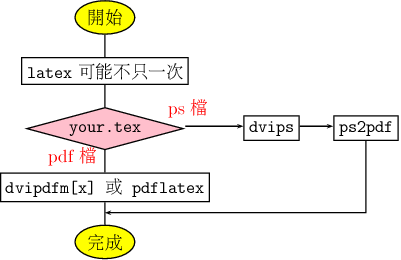
\includegraphics{latex-flow}
\end{center}

\section{\LaTeX{} 的特殊專用符號}

在 \TeX{}/\LaTeX{} 的世界,原始文稿都是純文字檔,任何一種編輯器都可以打開來編輯、觀看。而排版指令通常是由反斜線(\textbackslash, backslash)\index{反斜線}\index{backslash}所開頭來引導。註解\index{註解}則是由百分號(\texttt{\%})來引導。例如,以編輯器編輯下列文字:

\begin{quote}
   \begin{verbatim}
    This is my first \LaTeX{} typesetting example.
  \end{verbatim}
\end{quote}

編譯後會變成以下的結果:

\begin{quote}
   This is my first \LaTeX{} typesetting example.
\end{quote}

其中的 \verb|\LaTeX| 就是 \LaTeX{} 的一個指令,會顯示 \LaTeX{} 這個特殊的圖示。

由於,西方國家的語系,通常字母、符號的最大容量只有 256 個($2^8$),因此,許多現有的符號必須拿來當做控制指令,才能符合排版的多樣化需求。以下的符號,接觸 \TeX{}/\LaTeX{} 的朋友,可能都得時時留意,不要未經處理就直接寫進文稿裡頭去了。

通常,編輯器的語法顏色\index{語法顏色}會幫助判斷語法是否正確,但不是都能完美無缺,有時還是會漏掉,這時別忘了查看一下 {\ttfamily *.log} 檔案,例如:編譯 {\ttfamily your.tex} 檔的話,他的 log 檔就是 {\ttfamily your.log}。

\begin{quote}
   \begin{tabular}{llll}
      符號           & 作用                             & 文稿上使用              & \LaTeX{} 的替代指令     \\
      \hline
      \textbackslash & 下排版命令                       & \verb|$\backslash$|  & \verb|\textbackslash|  \\
      \%             & 註解                             & \verb|\%|  & NA                      \\
      \#             & 定義巨集                         & \verb|\#|  & NA                      \\
      \~{}           & 產生一個空白                     & \verb|\~{}|  & \verb|\textasciitilde|  \\
      \$             & 進入(離開)數學模式             & \verb|\$|  & \verb|\textdollar|  \\
      \_{}           & 數學模式中產生下標字             & \verb|\_{}| & \verb|\textunderscore| \\
      \^{}           & 數學模式中產生上標字             & \verb|\^{}| & \verb|\textasciicircum| \\
      \{             & 標示命令的作用範圍               & \verb|\{| & \verb|\textbraceleft| \\
      \}             & 標示命令的作用範圍               & \verb|\}| & \verb|\textbraceright| \\
      \textless      & 數學模式中的小於符號             & \verb|$<$| & \verb|\textless| \\
      \textgreater   & 數學模式中的大於符號             & \verb|$>$| & \verb|\textgreater| \\
      \textbar       & OT1 編碼,數學模式中才能正確顯示 & \verb+$|$+ & \verb|\textbar| \\
      \&             & 表格中的分隔符號                 & \verb|\&| & NA
   \end{tabular}
\end{quote}

\section{\LaTeX{} 排版上的一些規範或慣例}
\label{sec:convention}\index{規範}\index{慣例}

除了上面所談到的特殊符號外,也有一些規範或慣例要遵守,有些是比較硬性的規定,有些則只是慣例,可能不同的國家、語言會有不同的慣例,暫時先把他當成是 \LaTeX{} 的遊戲規則\index{遊戲規則}就成了。

\subsection{字型的相關術語}
\label{subsec:baseline}

要談排版上的規範、慣例前,我們得先認識一下字型的一些術語,以便往後文章中提到時有個概念。通常我們每個字都是置放於一個假想的方框中,稱為 em-square\index{em-square},同一個字型的同一個點數,每一個 em-square 大小都是相同的,實際上的字(glyph\index{glyph})要置放在這個 em-square 的什麼位置,這是字型設計者的觀點,所以,同樣點數的不同字型,他的字的大小不一定會一樣,因為我們是使用 em-square 的大小在比較的,而非實際的 glyph。

在文章中排列的時候,則是將 glyph 置於一個以假想參考點(reference point)\index{假想參考點}\index{reference point}為基準的一個假想線上,稱為基線(baseline\index{基線}\index{baseline}),大寫字母除了 Q 以外,他們的底部都是置於基線上的。但小寫字母則不一定剛好座落在基線上,有些字的筆畫可能超出基線以下,例如 y、j 等字母。關於字型在文章中的置放位置,我們來看看一個模擬圖:\footnote{實際字型設計上的各部份專有名詞及結構,當然不會是這麼簡略,這裡的模擬圖,只是暫時讓字的一般置放有個粗略的概念。}

% looks ugly, but l2h cannot handle this MP file be transparent png.
\begin{center}
   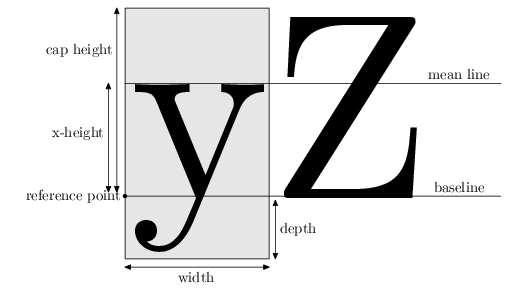
\includegraphics{baseline}
\end{center}

這個超出基線以下的長度,我們稱之為深度(depth\index{深度}\index{depth}),以上的就稱為字高(height\index{字高}\index{height}),當然大小寫的不同又分為大寫字母的字高(cap height\index{cap height})及小寫字母 x 的字高(x-height\index{x-height}),由於這個例子裡是調合字\index{調合字},所以每個字的寬度(width\index{寬度}\index{width})不一定會一樣,像打字機字族的則是等寬的字型。字高加上深度,我們就稱之為 totalheight\index{totalheight},大部份的情況,僅僅說 height 時是不包括 depth 的,而且通常指的是 cap height。

mean line\index{mean line} 在一般比較少用到,通常是字型設計\index{字型設計}時才會用到,他是指小寫字母去除上面突出的部份所連成的一個基準線,這個 mean line 到 baseline 的距離,一般就稱為 x-height,當然就是小寫字母 x 的高度,因此我們會有一個長度單位,稱為 ex,指的就是這個 x-height。

中文字的話比較特殊,他是以 em-square 的中心點來置放 glyph 的,在中英文混合時,中文字並不是剛好座落於基線上的,會超出基線下一點點,至於會超出多少,則和字型的設計有關,每種字型都有可能會不同。這也是為求排版上的一致性,字型可能都需要盡量使用同一套的各種字型的原因,否則就得經過微調,才能使整個字型表現上取得協調一致。

這些專門術語,往後提到一些指令的參數的描述時都會使用到,因此先熟悉一下,例如:字型旋轉時\index{字型旋轉},跟據的就是以參考點(reference point)為準,沿延伸出的軸心來旋轉的,而一般所說的行距\index{行距},指的是上下兩 baseline 的距離。

\subsection{一般性的遊戲規則}
\label{gen:gamerules}\index{遊戲規則}

\begin{enumerate}

   \item \LaTeX{} 的指令都是大小寫有別的,由 \verb|\| 開頭,後接由字母組成的字串或單一的非字母字元。其中由 \verb|[ ]| 中括號括住的是選擇性參數\index{選擇性參數},可以省略,由 \verb|{ }| 大括號括住的是不能省略的參數,當然,\LaTeX{} 的指令不一定會有參數,但絕大部份都會有參數,只不過把他給省略使用預設值罷了。

   \item \LaTeX{} 文稿中,空一個英文空白和空多個英文空白的作用是一樣,\LaTeX{} 會認作一個英文空白。

   \item 平常我們編輯純文字檔,按個 \textsf{Enter} 鍵,就代表換行,但實際排版出來,一行的寬度是按照排版版面的設定,也就是說,你在文稿中按 \textsf{Enter},不代表排版後就是從這裡斷行\index{斷行},\LaTeX{} 會依一行應有的寬度經過整體計算後自動補成一整行後再來斷行,而且會在中間自動補足一個空白。這在英文很自然,稱為字(word)間空白\index{字間空白},但中文則不一樣,在編輯器中編輯中文,隨意按 \textsf{Enter} 的結果,會造成文章中的中文間出現空白。這會在本文中適當的時機,提出解決的方法。

   \item 編輯器中,多按幾次 \textsf{Enter} 就多空出幾行,但在 \LaTeX{} 文稿裡,多個空白行\index{空白行},和一個空白行是一樣的作用,\LaTeX{} 會把他認作是一個空白行。而這個空白行,\LaTeX{} 同時也會認作是新段落的開始,所以 \LaTeX{} 是以空白行來分隔各個段落。

   \item \LaTeX{} 預設每個章節的第一個段落的第一行是不內縮(noindent\index{不內縮}\index{noindent}),從第二個段落開始才會內縮(indent\index{內縮}\index{indent})。當然,這是可以更改的,往後會再提及。

   \item \LaTeX{} 的指令,是從反斜線\index{反斜線}後第一個字母開始,到第一個非字母符號為止(包括空白、標點符號及數字)。因此:

         \begin{quote}
            \begin{verbatim}
      This is my first \LaTeX typesetting example.
    \end{verbatim}
         \end{quote}

         這樣的話,實際結果,因為 \verb|\LaTeX| 後的空白是屬於指令的一部份,空白將不會被解釋,這樣會印成:

         \begin{quote}
            This is my first \LaTeX typesetting example.
         \end{quote}

         這種結果,\LaTeX{} 和 typesetting 連在一起了。要避免的話,就要指定指令的作用範圍,例如以下的大括號。或就真的加個空白,例如 \verb|\ |,\LaTeX{} 碰到 \verb|\| 就會形成完整的指令,其後的空白就會被真正解釋為空白了:

         \begin{quote}
            \begin{verbatim}
      This is my first {\LaTeX} typesetting example.
      This is my first \LaTeX{} typesetting example.
      This is my first \LaTeX{} typesetting example.
    \end{verbatim}
         \end{quote}

         所以,正常印出來應該是:

         \begin{quote}
            This is my first \LaTeX{} typesetting example.
         \end{quote}

         % \index{\%@\verb=%=}
   \item 註解符號({\ttfamily \%})\index{註解符號}\index{%@\verb=%=},可以放在一行的任何地方,{\ttfamily \%} 後的文字會被 \LaTeX{} 忽略。所以,如果是放在一行的最尾端,那麼 \LaTeX{} 會自動插入的字間空白也將會被忽略。例如:

         \begin{quote}
            \begin{verbatim}
      This is my fisrt \LaTeX{} document. Give \LaTeX{} a%
try.
    \end{verbatim}
         \end{quote}

         這樣一來,排版出來會變成:

         \begin{quote}
            This is my fisrt \LaTeX{} document. Give \LaTeX{} a%
            try.
         \end{quote}

         a 和 try 連在一起了!正常應該是:

         \begin{quote}
            This is my fisrt \LaTeX{} document. Give \LaTeX{} a try.
         \end{quote}

         基於這個特性,我們可以應用在中文,也就是說在編輯器\index{編輯器}中,中文文章按 \textsf{Enter} 鍵換行時,尾端加個 {\ttfamily \%},這樣一來 \LaTeX{} 就不會插入英文字間空白,中文字就可以連成中間沒有空白的一整行了,否則 \LaTeX{} 在整篇文稿斷句\index{斷句}時,會自動在原換行處填入一個英文空白,因為,原始的 \TeX{}/\LaTeX{} 是認不得中文的。

   \item 中英文混合的時候,通常,英文字前後都會留個空白,以便和中文區隔開來,只是這個空白要多大,這就沒有固定的慣例,通常留個英文空白也是可以,要講究的話,等談到中文排版相關議題時再來討論,目前就養成習慣,英文單字前後留個英文空白。

\end{enumerate}

\subsection{針對標點符號的遊戲規則}

\begin{enumerate}

   \item 中英文的引號\index{引號}不一樣,這裡請特別注意,許多人常常搞錯。中、英文引號不管單雙都要分左右。英文的話,左邊的引號是 grave accent,是鍵盤左上方 {\sffamily Esc} 或 {\sffamily F1} 下方有波形號的那一個鍵;右邊的是 apostrophe\index{apostrophe},也就是鍵盤左邊 {\sffamily Enter} 鍵隔壁的那個鍵。雙引號的情形是鍵入兩次的左單引號\index{左單引號}及兩次的右單引號\index{右單引號},而不是用 \verb|"| 這個一次完成兩個點的 ditto marks\index{ditto marks}。所以,實際上在鍵入文稿時是:

         \begin{quote}
            \begin{verbatim}
Please press an `Esc' key.
Please press an 'Esc' key. 這是錯誤示範!
``This sentence.''
"This sentence." 這是錯誤示範!
\end{verbatim}
         \end{quote}

         排版出來的情形是:

         \begin{quote}
            Please press an `Esc' key.\\
            Please press an 'Esc' key. 這是錯誤示範!\\
            ``This sentence.''\\
            "This sentence." 這是錯誤示範!
         \end{quote}

         中文的話,我們是使用中文全形的「、」及『、』,在中國大陸則已改用和英文相同形狀的全形符號,但這在中文直排時會出問題,因此,中文的單、雙引號還是得維持我們目前使用的。

   \item \LaTeX{} 會在英文文章的一個句子結束和另一個句子開始的中間,自動調整成較大一點的空白,這可以增加文章的易讀性。所謂一個句子結束,例如:句點(.)、問號(?)、驚嘆號(!)及冒號(:),這當然是指英文的半形標點符號,不是中文的全形標點符號。你可以注意一下上面所舉的例子,在 document.\ 和 Give 之間的空白會稍微大於其他英文單字間的空白。

         現在的問題是,如果這些標點符號後面不是另一個句子的開始的時候,\LaTeX{} 無法去判斷這種情形,這時得由我們自己自行判斷、處理了。例如英文縮寫字:

         \begin{quote}
            \begin{verbatim}
I am Mr. Edward G.J. Lee, G.J. is a abbreviation of my name.
I am Mr.~Edward G.J. Lee, G.J. is a abbreviation of my name.
I am Mr.\ Edward G.J. Lee, G.J. is a abbreviation of my name.
\end{verbatim}
         \end{quote}

         其中 \verb|Mr.\ Edward| 的寫法,和 \verb|Mr.~Edward| 幾乎是一樣的,都是強迫插入一個比較小的正常單字間空白\index{單字間空白},差別在於後者也另外表示不可以從這裡換行,通常用在人名的時候,讓他們不致中斷,一般在人名的排版,包括他的頭銜、職稱,是不中斷成兩行而分開的。而且整個文句較長的話,以後者較恰當,才不會因為斷行被分成兩半,這個 {\ttfamily ~} 符號也因此在 \TeX{} 的專有名詞,就稱為 tie\index{tie},把他們綁住的意思。排版出來的時候會變成:

         \begin{quote}
            I am Mr. Edward G.J. Lee, G.J. is an abbreviation of my name.\\
            I am Mr.\ Edward G.J. Lee, G.J. is an abbreviation of my name.
         \end{quote}

         請放大去仔細比較一下結果就知道了。第二行的才是正確的,Mr.\ 和 Edward 之間的空白是正常單字間空白,比第一行的句子結束空白要小一點點。其他有使用到縮寫字的場合,例如:`Dr.'、`etc.'、`e.g.'、`i.e.'、`vs.'、`Fig.'、`cf.'、`Mrs.',這些都不是代表句子結束,所以,要插入一個正常空白。

         那 G.J. 後面為什麼沒有插入正常空白?那是因為,J 是大寫的,這時 \LaTeX{} 不會去誤認為是句子結束,通常句子結束時的句點前的那個字母是小寫的。Well,有沒有覺得有點道理?:-)

         等等,事情還沒有結束!Knuth 教授出了一道考題,如果句子的結束是 `Please see Appendix A.' 後面又還接有另一個句子。這時怎麼辦?由於,不會認為是句子結束,因此會插入正常空白,但這正是句子結束呀!請暫時先記得,使用 \verb|...Appendix A\null.|,或 \verb|...Appendix A\@.|。這個說來有點話長,有機會再來探討,請記得 `\verb|\null|' 和句點間是沒有空白的。例如:

         \begin{quote}
            \begin{verbatim}
Please see Appendix A. We will be there soon.
Please see Appendix A\null. We will be there soon.
\end{verbatim}
         \end{quote}

         排版出來的結果將會是(差異不明顯,請小心比較):

         \begin{quote}
            Please see Appendix A. We will be there soon.\\
            Please see Appendix A\null. We will be there soon.
         \end{quote}

         如果,你現在閱讀的是 HTML\index{HTML} 格式文件,有些例子如果無法明顯顯示出來,請改閱覽 PDF 版本。而且,如果你製作 PDF 格式時,字型沒有內嵌(本文的英數字是嵌入 Computer Modern Type1 字型),差異可能將會更不明顯。可試著使用 {\sffamily gv/gsview}\index{gv@\textsf{gs}}\index{gview@\textsf{gview}} 去閱覽,然後調整成 Landscape\index{Landscape},把句子尾部拉到邊緣的地方去就看得出來了。這在句子多的時候,這個空白也並非固定大小的,\LaTeX{} 會視文章結構的需要做細微的調整。

   \item 刪節號\index{刪節號}中文英也是不同,英文是三點,如果碰到句點的話,則是四點。中文的話是六點,碰到中文句點很容易就分得清楚。但是英文這個三點,不是就打個三個句點了事,這樣的點太密集,可以使用 \verb|\ldots| 或 \verb|\dots| 指令,例如:

         \begin{quote}
            \begin{verbatim}
I'm not a good man ..., but a good husband .... 錯誤示範!
I'm not a good \ldots\ man \ldots, but a good husband \ldots.
I'm not a good \dots\ man \dots, but a good husband \dots.
\end{verbatim}
         \end{quote}

         排版出的來結果是:

         \begin{quote}
            I'm not a good ... man ..., but a good husband .... 錯誤示範!\\
            I'm not a good \ldots\ man \ldots, but a good husband \ldots.\\
            I'm not a good \dots\ man \dots, but a good husband \ldots.
         \end{quote}

         中文的刪節號是由兩個全形的三點所組成六點的,即:\chdots{},就是我們 Big-5 碼的 {\ttfamily 0xa14b}({\ttfamily U+2026}),但由於 Unicode\index{Unicode} 尚有一個 MIDLINE HORIZONTAL ELLIPSIS({\ttfamily U+22EF}),因此,有些軟體在解讀上有可能會不一樣,因為我們的字型,大部分在製作標點符號時是置在中央的地方,不像中國大陸是置放在基線的地方,而 Unicode 官方採用的樣本字型,剛好是中國大陸的廠商所提供,這樣一來有些軟體工作者就認為我們的刪節號應該是 {\ttfamily U+22EF} 了,很不幸的,我們的 Big-5\index{Big-5} 碼並沒有相對應的字碼。

   \item 破折號\index{破折號}。在英文,相當於破折號的可能有三種:
         \begin{itemize}
            \item hyphen\index{hyphen} \newline
                  這是最短的 dash\index{dash},通常就是鍵入 \verb|-| 就行了,例如 \verb|father-in-low|,這樣會表現成 fater-in-low。

            \item en-dash\index{en-dash} \newline
                  這是最常用的破折號,是鍵入兩個 hyphen。例如 \verb|1991--2003 年|,這會表現成 1991--2003 年。

            \item em-dash\index{em-dash} \newline
                  這是最長的 dash,由三個連續的 hyphen 組成,應該是最相近於我們中文所說的破折號。例如 \verb|I am---a good man.| 會表現成 I am---a good man.。至於這個三個連續的 hyphen 前後是否要留空白,都有人使用,並沒有硬性的慣例,但為了和中文的破折號配合(中文破折號前後,通常不留空白),個人通常是不留空白的。

            \item 真正的減號 \newline
                  這應不能算是破折號,而是實際的減號或負號,這要進入數學模式,例如:負五,要寫成 \verb|$-5$|,然後表現出來是 $-5$。這也常常會有人搞錯,不能直接鍵入一般的負號那個鍵來充數,這是因為 \TeX{}/\LaTeX{} 的數學式子的用字和間隔處理,和一般內文不同的關係。

            \item 中文的破折號 \newline
                  中文的破折號是佔兩個中文字位置的的一橫線,長度和刪節號相同。在中線位置的,定義上是有兩種,en-dash 是 {\ttfamily Big-5 0xa156},em-dash 是 {\ttfamily Big-5 0xa158}。但由於中文字間距的問題,有可能打出來的破折號中間會有一點空白\footnote{這是可以調整的,也就是去除兩個橫線之間的字間距,這樣就不會產生小空白了,中文刪節號也有同樣的情形,我們會在微調的部份再來討論。},例如——中文的 em-dash,這是––中文的 en-dash。在論文中,破折號通常可以使用小括號或冒號代替。

            \item 中文的私名號及書名號 \newline
                  中文的私名號\index{私名號},可以標明人名、地名,如\underline{孫逸仙};書名號\index{書名號}(私名號的底線換成波紋形狀),可以用在書名,這些符號常造成排版上的困擾,常使用 《 》來取代書名號,私名號則無其他取代方法。在一般的自然及應用科學論文上通常不使用這種舊式的私名號及書名號。
         \end{itemize}

   \item 避頭點\index{避頭點} \newline
         這可是排版的重要功能。英文的通常沒有問題,\LaTeX{} 會自動避開處理,中文就不一定了,\LaTeX{} 可不認識中文,但通常中文相關程式及套件,多多少少都會處理,只不過,有時候偶爾可能會誤判。那麼,到底什麼是避頭點?底下列個表,大家就明白了,我列中文的,英文的就不列出來了,因為 \LaTeX{} 會自動處理,不必我們擔心。

         \begin{quote}
            \begin{tabular}{ll}
               標點符號            & 置放處       \\
               \hline
               ,。;、:」)》!? & 不能置於行首 \\
               「(《              & 不能置於行尾 \\
               破折號及刪節號      & 置於首尾皆可 \\
            \end{tabular}
         \end{quote}

         簡單的說,除了破折號及刪節號,沒有開口的,不能置於最開頭,開口向右的,不能置於最右,開口向左的,不能置於最左。通常都會處理好,但校稿的時候要注意一下誤判的地方。

\end{enumerate}

\section{\LaTeX{} 的文稿結構}
\label{sec:struct}\index{文稿結構}

\subsection{環境(environment)\index{環境}\index{environment}}

上一節所談的都是指令,雖然也可以由大括號\index{大括號}來定作用範圍,但如果是一整段,甚至是一整篇文章都要作用時,那指令可能就不很適合了,因此,\LaTeX{} 也有一種巨集結構,稱為環境(environment),主要是讓作用範圍能擴大至較大的範圍。

所有的環境,都是起於 \verb|\begin{環境名稱}|,止於 \verb|\end{環境名稱}|,這兩個指令之間的文稿都會被作用,而且,環境之內還可以套用其他不同的環境。

\LaTeX{} 文稿的內文,其實就是包在一個 \verb|\begin{document}| 和 \verb|\end{document}| 這個 document 環境當中。

\subsection{最簡單的 \LaTeX{} 的文稿結構}

以下就是所有 \LaTeX{} 必需具備的文稿大結構:

\begin{quote}
   \begin{verbatim}
\documentclass{article}

  這裡是 preamble 區

\begin{document}

  這裡是本文區

\end{document}
\end{verbatim}
\end{quote}

\verb|\documentclass{article}|,這是在告訴 \LaTeX{} 使用哪一種類別,我們目前使用的是 {\ttfamily article} 類別\index{類別}\index{article},關於類別會在第 \ref{ch:class} 章討論。preamble\index{preamble} 區,則是下一些會影響整個文稿的指令,及引用巨集套件的地方,當然,完全不引用巨集,也不使用影響全文的指令的話,preamble 區就是空白,不寫任何東西。本文區,就是我們實際上寫文章的地方。

現在也可以把前面所舉的例子,放入本文區裡頭,preamble 區空白沒關係,然後存檔,試著編譯看看:

\begin{quote}
   \begin{verbatim}
latex example.tex
dvips example.dvi      => 產生 ps 格式 example.ps
dvipdfm[x] example.dvi => 產生 pdf 格式
pdflatex example.tex   => 直接由 .tex 產生 .pdf
\end{verbatim}
\end{quote}

真正的實例解說,會在下一章來進行,所以,這裡暫時不會介紹有什麼環境可以使用,先玩看看沒有關係。由於還沒談到中文的問題,因此如果你想試試看,那暫時先使用英文,道理都是相通的。

\subsection{preamble 區可以放些什麼?}
\label{subsec:preamble}

這裡可以引用巨集,而且會影響整篇文稿的指令,例如一些事先定義好的指令,想在整篇文稿中使用,就可以置放在 preamble 區。

\subsubsection{巨集的引用}
\label{subsubsec:package}

本文主要是標準 \LaTeX{},但前面已提到,會有些巨集套件不得不要引用,底下就來說明如格引用套件。這些套件都是一般 \TeX{} 系統都會附上的。

指令及環境要如何開頭都介紹過了,現在來看看引用巨集要怎麼開頭。

\begin{quote}
   \begin{verbatim}
\documentclass{article}
\usepackage{color}
\begin{document}
\textcolor{blue}{This is blue color.}
\end{document}
\end{verbatim}
\end{quote}

編譯一下,看看結果是什麼?這裡使用的就是 \textsf{color} package\index{color@\textsf{color}},裡頭是由 \TeX{}/\LaTeX{} macro 所寫成一個巨集套件。一般簡單的我們就稱為巨集(macro)\index{巨集}\index{macro},複雜一點的就稱為巨集套件(package)\index{巨集套件}\index{package},其實,裡頭都是一樣的,只不過大小及有沒有整理成一個系統的差別。

\LaTeX{} 裡頭有什麼現成的套件可以使用,每個散佈的 \TeX{} 系統所收集的可能都會有所不同。大概沒有人可以精通所有現存的 \LaTeX{} 巨集套件,因為實在是太多了,不過,本文大概都會提到常用的巨集套件。詳細的巨集套件的種種,會在第 \ref{ch:package} 章來說明。

\subsubsection{影響整篇文稿的指令}

會影響整篇文稿的指令,通常也是放在 preamble 區,例如:

\begin{quote}
   \begin{verbatim}
\linespread{1.36}
\parindent=0pt
\end{verbatim}
\end{quote}

\verb|\linespread| 是在控制上下行的行距,這裡就是將行距變成原來的 1.36 倍。至於什麼是行距呢?就是這一行的基線(baseline)到下一行的基線的距離,通常英文文章不必去調整他的行距,但中文得適當加大行距以利閱讀。

\verb|\parindent| 是調整段落內縮的程度,這裡調整成 0,也就是說各段落都不內縮的意思,也可以調整成其他的值,\LaTeX{} 就會依這個值去內縮。當然,不去設定的話,\LaTeX{} 就會依他的預設值去內縮。

\subsection{章節結構\index{章節結構}}
\label{subsec:chapstruc}

本文區當然是我們寫文章的主要地方,及一些微調\index{微調}。在 \LaTeX{} 的文稿裡頭,章節標題的形成都是由同樣的指令來控制的,這樣有一個好處,臨時插入章節標題及其內文時,我們不必去理會標題編號及目錄的問題,也不必去理會要用什麼字型、及字型大小要多大,\LaTeX{} 會自動計算處理,字型大小也會和內文使用的字型大小互相配合調整,使用者就專心在內文構思、寫作即可。以下由列表來瞭解整個章節結構:

\begin{quote}
   \begin{tabular}{lll}
      深度標號 & 指令                    & 作用及注意事項                           \\
      \hline
      $-1$     & \verb|\part{}| & 這是最大的結構,我們中文通常稱為「部」。 \\
      0        & \verb|\chapter{}| & 章。在 article 類別裡頭沒有章。          \\
      1        & \verb|\section{}| & 節。                                     \\
      2        & \verb|\subsection{}| & 小節。                                   \\
      3        & \verb|\subsubsection{}| & 次小節。                                 \\
      4        & \verb|\paragraph{}| & 段落。                                   \\
      5        & \verb|\subparagraph{}| & 小段落。                                 \\
   \end{tabular}
\end{quote}

章節標題\index{章節標題}的內容就是直接寫入指令的大括號裡頭就可以了,\LaTeX{} 在排版時會自動使用粗體、加入章節編號\index{章節編號}及納入目錄\index{目錄}裡頭。

至於第一欄的深度標號(secnumdepth)\index{深度標號}\index{secnumdepth},{\ttfamily book/report}\index{book@\texttt{book}}\index{report@\texttt{report}} 類別的深度標號是 2,{\ttfamily article} 的是 3。這是什麼意思呢?就是說 {\ttfamily book/report} 類別的文稿,在 \verb|\subsection{}| 以後({\ttfamily subsection} 本身仍會編號),章節就不再編號了;同樣的,在 {\ttfamily article} 類別的文稿,在 \verb|\subsubsection{}| 以後就不編號了。但仍然會獨立出一單獨行來表示這個是標題。不編號了的章節內容,當然也就不納入目錄裡頭了。這當然是可以更改的,只要更改 \LaTeX{} 的 {\ttfamily secnumdepth} 這個變數的值就可以了,這個往後會提及如何更改 \LaTeX{} 的預設值。像這篇文章,在 preamble 區就有一個設定:

\begin{quote}
   \begin{verbatim}
% let the depth of report to subsubsection
\setcounter{secnumdepth}{3}
\end{verbatim}
\end{quote}

所以,這篇文章雖然使用的是 {\ttfamily report} 類別,但是章節的深度標號是標在 3,也就是說會編號到 {\ttfamily subsubsection} 為止,但這仍然是沒有編入目錄中的。

下一章就讓我們開始實際動手吧!但 \chdots{},怎麼到現在都沒有完整介紹指令呢?那我怎麼會知道有什麼指令可以使用?這是因為 \LaTeX{} 的指令很多,直接介紹的話,一方面記不住,二方面也不容易瞭解他的實際作用,所以,我們將會在下章舉例時穿插在裡頭說明,等這份文件接近尾聲時,再來整理個指令速查表,這樣以後查指令就很方便了,不必去死記,只要知道有個這樣功能的指令就夠了。

  % syntax.tex
% !TeX root = ../main.tex

\chapter{實際上排版玩看看}
\label{ch:start}

好了,現在正式來玩看看吧!本章主要是簡單的實例說明,先進入狀況再談其他。實際應用比高談闊論有用多了。

先來個「最高指導原則」:\textcolor{red}{\bfseries 學會控制空間,你就學會排版了}!剛學排版的朋友,往往會把所學到的東西去想法子佈滿你所有的空間(就是一個頁面),但實際上,你要調整的,其實是各個部份的空間配置,抽象一點說,也就是一整個頁面當中,沒有文字、圖表的部份才是排版真正的重點。你先聽聽就好,過一段時間的熟悉後,再來回頭思考這個「玩弄」空間的原則。:-)

由於本文有 HTML 版本,為了轉換上不造成失真,實例的部份,文稿上只寫程式碼,結果的部份都是編譯好的 PDF 格式檔案,置放於網站上,可線上閱覽或下載,簡單的例子則不另製作獨立的 PDF 檔,請參閱本文的 PDF 格式檔案內容。

\section{簡單的實例}

這裡就把前一章所談到的一些內容整理成一個文稿,先來試試看,這裡先使用 {\ttfamily report}\index{report@\texttt{report}} 類別文稿,因為 {\ttfamily article}\index{article@\texttt{article}} 類別文稿是沒有 {\ttfamily chapter} 的:

\begin{quote}
   \begin{verbatim}
% example1.tex
\documentclass{report}
\begin{document}
This is my first {\LaTeX} typesetting example.\\
This is my first \LaTeX{} typesetting example.\\
This is my first \LaTeX{} typesetting example.\\
I am Mr. Edward G.J. Lee, G.J. is a abbreviation of my name.\\
I am Mr.\ Edward G.J. Lee, G.J. is a abbreviation of my name.\\
Please see Appendix A. We will be there soon.\\
Please see Appendix A\null. We will be there soon.
\end{document}
\end{verbatim}
\end{quote}

使用編輯器編輯,然後存檔成 {\ttfamily exmaple1.tex},這樣就可以編譯了:

\begin{quote}
   \begin{verbatim}
latex example1.tex       => 產生 example1.dvi
dvips -Ppdf example1.dvi => 產生 example1.ps
ps2pdf example1.ps       => 產生 example1.pdf 或
dvipdfm[x] example1.dvi  => 由 example1.dvi 直接產生 example1.pdf 或
pdflatex example1.tex    => 由 example1.tex 直接產生 example1.pdf
\end{verbatim}
\end{quote}

編譯好的 PDF 檔可在此下載或閱覽:

\begin{quote}
   \url{http://edt1023.sayya.org/tex/latex123/example1.tex}  \\
   \url{http://edt1023.sayya.org/tex/latex123/example1.pdf}
\end{quote}

\subsection{關於換行}

每行最後加了個 \verb|\\|\index{\\@\verb=\\=},這表示強迫換行的意思,否則 \LaTeX{} 會依版面預設的寬度來換行,就不會是一個句子一行了,大家可以把這個 \verb|\\| 拿掉,再來編譯試看看結果,就會知道怎麼一回事了。也可以使用 \verb|\newline|\index{newline@\verb=\newline=} 這個指令,當然,我們都會聰明的選用較短的指令。而且 \verb|\\| 可以控制換行時的間隔,這在 \verb|\newline| 則不行。例如:

\begin{quote}
   \begin{verbatim}
Please see Appendix A. We will be there soon.\\[1cm]
Please see Appendix A\null. We will be there soon.
\end{verbatim}
\end{quote}

這樣的話,兩行之間的行距\index{行距}就是原來的行距再加上 {\ttfamily 1cm}。甚至,也可以是負數的參數,這樣行距就會變成原來的行距減去 {\ttfamily 1cm},當然,如果設過頭了的話,兩行可能會重疊在一起。既然,這裡使用的是方括號,表示這些參數是可以省略的。

另外,\verb|\linebreak[n]|\index{linebreak@\verb+\linebreak+} 也可以強迫換行\index{強迫換行},{\ttfamily n} 代表由 1--4 的建議值,數值愈大表示愈是強烈建議,不設定的話,就是換或不換兩種選擇,沒有中間地帶。和前面所說的不同處是,這種換行會把原來那一行句子的長度平均布滿版面上行寬的長度。例如:

\begin{quote}
   \begin{verbatim}
Please see Appendix A. We will be there soon.\linebreak
Please see Appendix A\null. We will be there soon.
\end{verbatim}
\end{quote}

排版後會表現成:

\begin{quote}
   Please see Appendix A. We will be there soon.\linebreak
   Please see Appendix A\null. We will be there soon.
\end{quote}

\subsection{關於縮排\index{縮排}}

第一行縮排了!這是因為我們完全沒有分章節,所以,\LaTeX{} 就把這些內容當做是引言的部份,依 \LaTeX{} 的安排,引言開頭是會縮排的。要解決這個問題,可有兩種方法:

\begin{enumerate}
   \item 在第一行之前加入 \verb|\noindent|\index{noindent@\verb+\noindent+} 來指示 \LaTeX{} 不要去縮排。但是這只作用在下指令的地方,其他該縮排的地方還是會縮排。
   \item 在 preamble 區加入 \verb|\parindent=0pt|\index{parindent@\verb+\parindent+},這表示讓全文的縮排為 {\ttfamily 0pt},當然,這就表示全文都不要縮排了。
\end{enumerate}

\section{加入章節標題\index{章節標題}}

在 \LaTeX{} 裡頭,要加入章節標題實在是太容易了,也不必去管字體的大小及置放的位置,盡管加上去就對了!\LaTeX{} 會替我們安排一切。我們這裡仍然以 {\ttfamily report} 類別來說明,因為 {\ttfamily article} 類別裡頭,沒有章,只能適用於較簡單的短文。

\begin{quote}
   \begin{verbatim}
% example2.tex
\documentclass{report}
\begin{document}
This is the first experience of \LaTeX.
\chapter{Aesop Fables}
\section{The Ant and the Dove}
An ant went to the bank of a river to quench its thirst, and
being carried away by the rush of the stream, was on the
point of drowning.
A Dove sitting on a tree overhanging the water plucked a
leaf and let it fall into the stream close to her. The Ant
climbed onto it and floated in safety to the bank.
\section{The Dog in the Manger}
A dog lay in a manger, and by his growling and snapping
prevented the oxen from eating the hay which had been
placed for them.
``What a selfish Dog!'' said one of them to his companions;
``he cannot eat the hay himself, and yet refuses to allow
those to eat who can.''
\chapter{The Eagle and the Arrow}
An eagle sat on a lofty rock, watching the movements of a
Hare whom he sought to make his prey.
An archer, who saw the Eagle from a place of concealment,
took an accurate aim and wounded him mortally.
\end{document}
\end{verbatim}
\end{quote}

編譯出來的結果:

\begin{quote}
   \url{http://edt1023.sayya.org/tex/latex123/example2.tex}\\
   \url{http://edt1023.sayya.org/tex/latex123/example2.pdf}
\end{quote}

請注意他什麼時候會縮排,什麼時候會換頁。{\ttfamily report} 類別,新的一章會換頁,如果想節省一點空間,可以換用 {\ttfamily article} 類別,\verb|\chapter{}| 改用 \verb|\section{}|,原來 \verb|\section{}| 就改用 \verb|\subsection{}|,這樣就不會換頁,內容就會連續下去了。大家可以試著把 {\ttfamily report} 改成 {\ttfamily article} 及 {\ttfamily book} 再重新編譯一次,試試看結果有何不同。

\section{加入 title page 資訊}
\label{sec:titlepage}\index{title page}

這是指內頁的第一頁,我也不知道這個中文專有名詞是什麼,在 \LaTeX{} 裡頭,我們就稱為 title page。在 \LaTeX{} 的標準格式裡,他包括了標題(title)、作者名字(author)、日期(date\index{date})及感謝詞(thanks\index{thanks})。要注意的是,在 {\ttfamily report/book} 類別,title page 是自成一單獨頁的,但在 {\ttfamily article} 類別裡,他是和本文連起來的。我們就以上面的伊索寓言的文章為例,要修改的地方是 preamble\index{preamble} 區及本文區的 \verb|\maketitle|\index{\verb=\maketitle=}:

\begin{quote}
   \begin{verbatim}
% example3.tex
\documentclass{report}
\title{Aesop Fables}
\author{Aesop\thanks{Thanks to the reader.}
      \and Nobody\thanks{Thanks to nobody.}}
\date{\today}
\begin{document}
\maketitle
This is the first experience of \LaTeX.
\chapter{Aesop Fables}
\section{The Ant and the Dove}
 ...
\end{verbatim}
\end{quote}

排版出來的結果如下:

\begin{quote}
   \url{http://edt1023.sayya.org/tex/latex123/example3.tex}\\
   \url{http://edt1023.sayya.org/tex/latex123/example3.pdf}
\end{quote}

我們可以發現,這一頁是不編頁碼的,從下一頁開始才是第一頁。作者可以有多個,使用 \verb|\and| 指令來連接。日期不一定要有,如果沒有 \verb|\date{\today}| 這個指令,那還是有日期,但只能固定在今天。如果內容過長,他會自動折行,但也可以手動加 \verb|\\| 來強迫換行,不管如何換行,整個句子是居中排列的。\verb|\maketitle| 是下在本文區的開頭,如果不下這個指令,那編譯時不會有什麼錯誤,只是就沒有 title page 了。

\section{加入目錄(Table of Contents)}
\label{sec;toc}

加入目錄(Table of Contents\index{Table of Contents})對 \LaTeX{} 而言,更是輕而易舉的事情,只要在本文開頭加個
\verb=\tableofcontents=\index{tableofcontents@\verb=\tableofcontents=}
指令就成了!依上面的例子,修改成:

\begin{quote}
   \begin{verbatim}
% example4.tex
\documentclass{report}
\title{Aesop Fables}
\author{Aesop\thanks{Thanks to the reader.}
      \and Nobody\thanks{Thanks to nobody}}
\date{\today}
\begin{document}
\maketitle
\tableofcontents
This is the first experience of \LaTeX.
\chapter{Aesop Fables}
\section{The Ant and the Dove}
 ...
\end{verbatim}
\end{quote}

排版出來的結果如下:

\begin{quote}
   \url{http://edt1023.sayya.org/tex/latex123/example4.tex}\\
   \url{http://edt1023.sayya.org/tex/latex123/example4.pdf}
\end{quote}

這裡千萬要注意的是,\verb|\tableofcontents| 要加在 \verb|\maketitle| 的後面,否則目錄會印在 title page 之前。而且要\textcolor{red}{\bf 編譯兩次}。第一次產生 {\ttfamily example4.toc},然後第二次編譯再跟據這個 {\ttfamily toc} 檔,真正編入目錄。

目錄是包括圖表目錄的(List of Figures, List of Tables),但我們目前還沒有談到圖表的排版,因此暫時略過,等談到時再來看要如何加入圖表目錄。

\section{加入摘要(abstract)}
\label{sec:abstract}\index{abstract}

這不一定會有,如果要加入的話,可使用 {\ttfamily abstract} 環境,在這個環境中的文章,左右會縮排。要注意的是,只有 {\ttfamily article/report} 類別才有 abstract,{\ttfamily book} 類別不能使用這個環境。

\begin{quote}
   \begin{verbatim}
% example5.tex
\documentclass{report}
\title{Aesop Fables}
\author{Aesop\thanks{Thanks to the reader.}
      \and Nobody\thanks{Thanks to nobody}}
\date{\today}
\begin{document}
\maketitle
\begin{abstract}
The tale, the Parable, and the Fable are all common and popular
modes of conveying instruction. Each is distinguished by its own
special characteristics.
\end{abstract}
\tableofcontents
\chapter{Aesop Fables}
\section{The Ant and the Dove}
 ...
\end{verbatim}
\end{quote}

排版出來的結果如下:

\begin{quote}
   \url{http://edt1023.sayya.org/tex/latex123/example5.tex}\\
   \url{http://edt1023.sayya.org/tex/latex123/example5.pdf}
\end{quote}

{\ttfamily report}\index{\texttt{report}} 類別的摘要自成一頁,不編頁碼,且不會編入目錄中,這和一般的論文格式可能會不一樣,使用時請注意。{\ttfamily artcile}\index{\texttt{artcile}} 的類別則仍然是和本文相連的,會出現在文章標題之後。

{\ttfamily abstract} 和 summary\index{summary} 在較正式的論文是有區分的,通常 abstract 在文前;summary 則在文後。但目前一般性的文章則沒有這樣區別,通通當成「摘要」。通常,摘要裡頭是不用註解、無交互參照也不使用公式圖表的。


\section{加入註解}
\label{sec:footnote}\index{註解}

在 \LaTeX{} 裡頭,註解可有兩種方式,一種是腳註(footnote)\index{footnote}\index{腳註},一種是邊註(marginal note)\index{marginal note}\index{邊註}。通常 \LaTeX{} 的腳註預設是由阿拉伯數字在編號,置於頁底部。在沒有部(part)的情形下,\texttt{report/book} 類別,編號每章會從頭起算,\texttt{article} 類別則會連續,而且,會使用 \texttt{footnotesize}\index{footnotesize@\texttt{footnotesize}} 的字體印出。邊註則不編號,字體是正常大小。

\subsection{腳註(Footnote)}

在所要加註的那個字後,使用 \verb|\footnote{}| 指令即可,解說的文字就寫入大括號之內,一般 \LaTeX{} 的指令在此都仍然有有作用,會印在此頁的底部,以小一點的字來印出,並加上編號。以下我們就試試看在 Dove 這個字來做腳註。請注意,Dove 這個字和 \verb|\footnote{}| 之間是沒有空白的。

\begin{quote}
   \begin{verbatim}
% example6.tex
\documentclass{report}
\title{Aesop Fables}
\author{Aesop\thanks{Thanks to the reader.}
      \and Nobody\thanks{Thanks to nobody}}
\date{\today}
\begin{document}
\maketitle
\tableofcontents
This is the first experience of \LaTeX.
\chapter{Aesop Fables}
\section{The Ant and the Dove}
An ant went to the bank of a river to quench its thirst, and
being carried away by the rush of the stream, was on the
point of drowning.
A Dove\footnote{Pigeon, an emblem of peace.}
sitting on a tree overhanging the water plucked a
leaf and let it fall into the stream close to her. The Ant
climbed onto it and floated in safety to the bank.
 ...
\end{verbatim}
\end{quote}

排版出來的結果如下:

\begin{quote}
   \url{http://edt1023.sayya.org/tex/latex123/example6.tex}\\
   \url{http://edt1023.sayya.org/tex/latex123/example6.pdf}
\end{quote}

\subsection{邊註(Marginal note)}

邊註只是把 \verb|\footnote{}| 換成 \verb|\marginpar{}|\index{marginpar@\verb=\marginpar=} 而已,內容仍然寫入大括號內。但和腳註不一樣的是,他沒有編號(因為就在旁邊,無此必要),他的字體也不會小一號,和內文的字體大小是一樣的,這在後面討論到字型的時候會談到如何改變字體的大小。

\begin{quote}
   \begin{verbatim}
% example7.tex
\documentclass{report}
\title{Aesop Fables}
\author{Aesop\thanks{Thanks to the reader.}
      \and Nobody\thanks{Thanks to nobody}}
\date{\today}
\begin{document}
\maketitle
\tableofcontents
This is the first experience of \LaTeX.
\chapter{Aesop Fables}
\section{The Ant and the Dove}
An ant went to the bank of a river to quench its thirst, and
being carried away by the rush of the stream, was on the
point of drowning.
A Dove\marginpar{Pigeon, an emblem of peace.}
sitting on a tree overhanging the water plucked a
leaf and let it fall into the stream close to her. The Ant
climbed onto it and floated in safety to the bank.
 ...
\end{verbatim}
\end{quote}

排版出來的結果如下:

\begin{quote}
   \url{http://edt1023.sayya.org/tex/latex123/example7.tex}\\
   \url{http://edt1023.sayya.org/tex/latex123/example7.pdf}
\end{quote}

\section{字型的相關調整}
\index{字型!相關調整}

\TeX/\LaTeX{} 的字型系統算是相當複雜的,這裡不多談其中原理,站在使用者的角度,我們只要知道怎麼使用就行了。在這裡,我們說字型(font)\index{font}\index{字型},指的是字型本身的一個總稱,或稱為字體\index{字體},在字的形狀的時候,我們就稱為字形(font shape)\index{font shape}\index{字形}。

\LaTeX{} 使用的字型選字機制,以目前新版本的 \LaTeX{} 而言,是使用 1993 年發行的 NFSS(New Font Selection Scheme) 第二版為標準。當然,仍然是建立在 \TeX\ 字型機制的基礎上的,這已超出這篇文章的範圍。

\subsection{\LaTeX{} 對字型的屬性描述}
\label{subsec:font-attr}\index{字型!屬性描述}

在 \LaTeX{} 裡,對於字型的描述,使用了五種屬性來說明,這五種屬性,也是 \LaTeX{} 巨集中常要使用到的參數,甚至是錯誤訊息標示字型來源的時候,會把字型的這些屬性給顯示出來。

\begin{enumerate}
   \item 字型編碼(font encoding)\index{font encoding}\index{字型!字型編碼}\\
         這裡所謂的字型編碼,指的是各個個別的字在一個字型裡頭的排列順序及安排方式。原始的 \TeX\ 字型編碼我們就稱為 OT1(Old \TeX\ text encoding)\index{OT1},這是預設的,如果都不指定字型編碼,那所使用的就是 OT1 編碼。在目前新一代的字型編碼裡頭,字的安排方式及內容和 OT1 不一樣,例如
         T1\footnote{正式名稱是 Cork's \TeX\ extended text encoding 又稱為 Text Companion encoding。這裡的 T1 和 Type 1 字型規格\index{字型!字型規格}無關,他是字型編碼方式,他把字型裡頭有關一些重音符號字母單獨視為一個單獨的字,而非如 OT1 是由一般字母和重音符號組合而成。}\index{T1},這在往後提到改變字型編碼時會再談到,我們目前就不去調整字型編碼,使用預設的 OT1,其他的編碼這裡就不多談了。

   \item 字族(font family)\index{font family}\index{字族}\\
         指同一設計類型的字型集合的名稱,例如羅馬字族(roman)\index{roman}\index{羅馬字族}、打字機字族(typewriter)\index{typewriter}\index{打字機字族}等等,通常前面會冠上製作商或製作人的名稱,例如 Knuth\index{Knuth} 教授設計的,稱為 `Computer Modern Roman'\index{Computer Modern Roman},Adobe 公司製作的羅馬字族稱為 `Adobe Times'\index{Adobe Times}。我們預設使用的,當然就是 Knuth 教授所設計的 Computer Modern fonts。以下為一些例子:

         \begin{quote}
            \begin{tabular}{>{\ttfamily}ll}
               簡稱 & 代表意義                   \\
               \hline
               cmr  & Computer Modern Roman      \\
               cmss & Computer Modern Sans Serif \\
               cmtt & Computer Modern Typewriter
            \end{tabular}
         \end{quote}

   \item 字型系列(font series)\index{font series}\index{字型!字型系列}\\
         這是指字型的 weight(胖瘦)及 width(長扁)來區分的。例如粗、細字體,一般我們正常用的是 medium,粗體則是 bold。以下是一些例子:

         \begin{quote}
            \begin{tabular}{>{\ttfamily}ll}
               簡稱 & 代表意義      \\
               \hline
               m    & medium        \\
               b    & bold          \\
               bx   & Bold extended \\
               sb   & Semi-bold     \\
               c    & Condensed
            \end{tabular}
         \end{quote}

   \item 字形(font shape)\index{font shape}\index{字形}\\
         這個望文生義,就是字的形狀。例如意大利斜體(italic)\index{italic}\index{意大利斜體}、斜體(slant)\index{slant}\index{斜體}、small caps\index{small caps} 等等。以下是幾個例子:

         \begin{quote}
            \begin{tabular}{>{\ttfamily}ll}
               簡稱 & 代表意義                              \\
               \hline
               n    & 正常字(normal),指 upright 或 roman \\
               it   & Italic                                \\
               sl   & Slanted                               \\
               sc   & Small Caps                            \\
            \end{tabular}
         \end{quote}

   \item 字型大小(font size)\index{font size}\index{字型!字型大小}\\
         預設的字型大小是 10pt(10 point),十點字。不加單位的話,預設的就是 pt。請注意,非標準 \LaTeX{} 類別的預設字型大小可能會不一樣。
\end{enumerate}

我們對字型要調整改變的,就是這些字型屬性的設定值。\LaTeX{} 已設定好方便的指令給我們使用。

\subsection{調整字族、字型系列、字形的指令}
\label{subsec:font-command}

\linespread{1.0}
\small
\begin{tabular}[\textwidth]{lllll}
      & 字型                & 標準指令                & 宣告式指令(環境)      & 舊用法                  \\
   \hline
   字 & \textup{textup}     & \verb|\textup{textup}| & \verb|{\upshape textup}| &                         \\
   形 & \textit{italic}     & \verb|\textit{italic}| & \verb|{\itshape italic}| & \verb|{\it italic}| \\
      & \textsl{slant}      & \verb|\textsl{slant}| & \verb|{\slshape slant}| & \verb|{\sl slant}| \\
      & \textsc{small caps} & \verb|\textsc{small caps}| & \verb|{\slshape small caps}| & \verb|{\sc small caps}| \\
   \hline
   系 & \textmd{medium}     & \verb|\textmd{medium}| & \verb|{\mdseries medium}| &                         \\
   列 & \textbf{boldface}   & \verb|\textbf{boldface}| & \verb|{\bfseries boldface}| & \verb|{\bf boldface}| \\
   \hline
   字 & \textrm{roman}      & \verb|\textrm{roman}| & \verb|{\rmfamily roman}| & \verb|{\rm roman}| \\
   族 & \textsf{sans serif} & \verb|\textsf{sans serif}| & \verb|{\sffamily sans serif}| & \verb|{\sffamily sans serif}| \\
      & \texttt{typewriter} & \verb|\texttt{typewriter}| & \verb|{\ttfamilyfamily typewriter}| & \verb|{\ttfamily typewriter}| \\
\end{tabular}
\linespread{1.36}
\normalsize

先別嚇了一跳,這是有跡可循的。其中 upright, medium, roman 都是一樣的,這是一般的正常字,就不必麻煩去設定他了,除非是要在特定字型範圍裡頭,重新改變成正常字體。從前面所說的簡稱的字串,再和 text, family, series, shape 去配對來使用,這樣只要記得簡稱就行了,例如:italic 的就是 \verb|\textit{}|。不然也可以使用「偷吃步」的舊用法,其實這也不是什麼偷吃步,他是原始 Plain \TeX\index{Plain \TeX} 所定義的,在舊版的 \LaTeX{} 2.09 也相容他而沿用,並加以擴充。但如果使用舊用法,那有時組合式的表示時可能會無效,例如粗斜體這種粗體和斜體設定混合時,就無法產生粗斜體了,這時還是得乖乖使用正統標準 \LaTeX{} 的表示法。

要注意的是,大括號的位置,宣告式的指令,整個作用範圍是連指令一起包住的,他可以當成環境來使用,例如 \verb|\begin{itsahpe}|, \verb|\end{itshape}|,這樣在這個環境內的文字就通通會使用 italic 斜體,也可以不加參數使用,例如 \verb|\itshape|,這樣以下的文字通通會使用 italic 斜體,直至另一個改變字型的指令出現為止。標準指令的作用範圍則是當做指令的一個參數,這些參數是出現在指令後的大括號內的。現在就來實際編譯個例子試看看:

\begin{quote}
   \begin{verbatim}
% example8.tex
\documentclass{report}
\title{\bfseries Aesop Fables}
\author{Aesop\thanks{Thanks to the reader.}
      \and Nobody\thanks{Thanks to nobody}}
\date{\today}
\begin{document}
\maketitle
\tableofcontents
\chapter{Aesop Fables}
\section{The \textsl{Ant} and the \textsl{Dove}}
\itshape
An antwent to the bank of a river to quench its thirst, and
being carried away by the rush of the stream, was on the
point of drowning.
\upshape
A \textsl{Dove} sitting on a tree overhanging the water plucked a
leaf and let it fall into the stream close to her. The \textbf{\textsl{Ant}}
climbed onto it and floated in safety to the bank.
\section{The {\it Dog}\/ in the Manger}
A \textbf{\textit{dog}} lay in a manger, and by his growling and snapping
prevented the oxen from eating the hay which had been
placed for them.
``What a selfish Dog!'' said one of them to his companions;
``he cannot eat the hay himself, and yet refuses to allow
those to eat who can.''
\chapter{The \textsc{Eagle} and the Arrow}
An \textsc{eagle} sat on a lofty rock, watching the movements of a
Hare whom he sought to make his prey.
An archer, who saw the \textsc{Eagle} from a place of concealment,
took an accurate aim and wounded him mortally.
\end{document}
\end{verbatim}
\end{quote}

我們把 title page\index{title page} 的標題改成粗體(請注意,宣告式或舊用法,大括號是把指令和文字整個括住的),把 Dove 改成 slant 斜體,把 dog 改成 italic 粗斜體\footnote{請注意,這兩種斜體是不一樣的,slant 是一般正常的字,只是把他傾斜個角度而已,但 italic 則是另一種獨特的字型設計。},把 ant 改成 slant 粗斜體,把 eagle 改成 small caps。由於章節標題原本就會轉換成粗體,所以章節標題的部份,粗體就不必重複設了。

但這裡發現例子裡第二章標題中的 Eagle 並沒有改變字體,而且以 {\ttfamily latex} 編譯時會產生以下的錯誤(這些訊息也會在 {\ttfamily example8.log} 中找到):

\begin{quote}
   \begin{verbatim}
  ...
LaTeX Font Warning: Font shape `OT1/cmr/bx/sc' undefined
(Font)              using `OT1/cmr/bx/n' instead on input line 4.
  ...
LaTeX Font Warning: Some font shapes were not available, defaults substituted.
  ...
\end{verbatim}
\end{quote}

現在我們看到了前面所談的屬性簡稱,這在 \LaTeX{} 就會使用這種屬性來表示而發出訊息,這裡 \verb|OT1/cmr/bx/sc| 就表示了 OT1 編碼,Computer Modern Roman 字族,Bold extended 系列,而且是 small caps 形狀的字型,錯誤訊息顯示,他並沒有定義,因此,這個字型將會使用預設的字型來代替,這裡就是以 n 正常形狀的 bx 系列字型來替代。所以,字型指令並不是都可以隨意組合的,有些是根本就沒有這種字型,有些則是沒有用巨集去定義好,這樣 \LaTeX{} 就取不到字了,但別擔心,頂多就是使用預設的字型罷了!

另一個很奇怪的地方,就是第一章、第二節的標題,為什麼是 \verb|{\it Dog}\/ in the...}|?這個插入的 \verb|\/| 是什麼東西?這是 \TeX\ 系統調整斜體字(包括 iatlic 及 slanted)和正常字之間的空白的一個指令,稱為 italic correction\index{italic correction}。這樣,在斜體字和正常字之間的空白才會正常。那為什麼其他的斜體指令沒有加這個調整呢?這是因為 \LaTeX{} 巨集在設計時就有考慮到這個問題,所以 \verb|\textit{}| 這類標準指令都會自動調整 italic correction,不必由我們手動調整。

另外,章節標題本就會自動轉換成粗體,標題上的 dog 為什麼沒有變粗體?這在前面有提到過,這種舊用法有時是無法複合使用的,粗體又斜體的指令會用不上來。因此,建議盡量使用 \LaTeX{} 的第一種標準指令來改變字型。使用 \verb|{\it ...}| 或 \verb|{\itshape ...}|\footnote{宣告式指令可以複合使用,但仍然會需要手動做 italic correction。} 這種指令的話,就得時時注意 italic correction 的問題,也得注意是否可以複合使用指令的問題,所以,還是不要偷懶的好。:-)

後下是排版出來的結果:

\begin{quote}
   \url{http://edt1023.sayya.org/tex/latex123/example8.tex} \\
   \url{http://edt1023.sayya.org/tex/latex123/example8.pdf}
\end{quote}

\subsection{相對字型大小的調整}

接下來談最後一個字型大小屬性的調整,這在使用上比較單純,只要知道指令就可以馬上拿來使用。但是 \TeX{}/\LaTeX{} 系統中,談到字型,裡頭一堆地雷,例如前面談到正常的內文字型大小是 10pt,現在如果想製作海報,需要 64pt 的字的時候就會發現,設不出來了!正常 \LaTeX{} 的定義,字型的大小範圍是在 5--24.88pt 之間,超出這個範圍的字需要其他的 package 的幫忙。\footnote{這是 \LaTeX{} 本身巨集定義的問題,因為他主要是針對一般性文件及書籍,\TeX{} 本身的能力,可以讓字型放大到 2047pt。}

這裡我們先來看看內文 10pt 時各種字型大小指令、實際例子及其大小(這是相對大小,會隨內文預設字型大小而自動調整):\footnote{請注意,本文 pdf 格式內文使用 12pt 字型大小,列表及其中的例子,是由另外 10pt 預設字型大小所製作的 eps 圖檔引入,以免失真。}

\begin{quote}
   \centering
   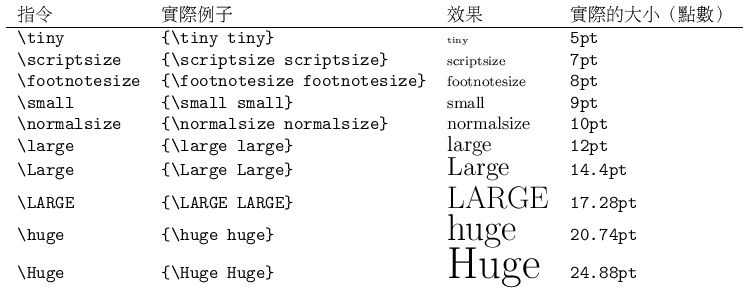
\includegraphics{fntsize}
\end{quote}

這些字型大小指令也可以當成環境來使用,例如:

\begin{quote}
   \begin{verbatim}
\begin{small}
  本文內容
\end{small}
\end{verbatim}
\end{quote}

這樣用也是可以的。

\subsection{絕對字型大小的調整}

通常字型的大小\index{字型!字型大小},使用上一節所說的相對字型大小來調整會比較方便,而且對於整個版面的配合也會比較恰當,例如行距也會跟著做適當的調整,如果自行用絕對字型大小的方法來調整字型大小的話,常常會造成行距不一致的情形,因此,如非必要,應盡量避免。

但有時候就是需要做這樣的調整,例如本文封面的字型大小,縱使是 \LaTeX{} 預設的最大字型也覺得稍小了點,這就要另外引入 package 調整了。

這裡我們使用 \textsf{type1cm}\index{type1cm@\textsf{type1cm}} package 來調整。當然,得使用 Type 1 字型,才可以達到無段放大、縮小的目的%
\footnote{\LaTeX{} 系統中的字型放大,在 10pt 以上,是以 1.2 的倍數為次方來放大的,因此,正文 10pt 的字型大小的話,不會有 13pt 這種大小的字型,\LaTeX{} 會選用最相近大小的字型來替代。}%
,而這個 package 也是配合 Type 1 字型使用的。個別放大的 pk 點陣字,這裡就不討論了,目前絕大部份的 Computer Modern 字型都已有 Type 1 的 free 版本,而且各個 \TeX\ distribution 都會附上,使用上會較方便。以下是 \textsf{type1cm} 的使用方法:

\begin{quote}
   \begin{verbatim}
  ...
\usepackage{type1cm}
  ...
\fontsize{字型大小}{行距大小}\seclectfont
  ...
\end{verbatim}
\end{quote}

還記得如何引用巨集套件\index{巨集套件}嗎?請參考第 \ref{ch:syntax} 章、第 \ref{sec:struct} 節,第 \ref{subsec:preamble} 小節的說明。

其中的「字型大小」就是所要指定的大小,通常以 pt 為單位,當然,要使用其他單位也是可以。「行距大小」也是要一併指定,不可省略。最後的 \verb|\seclectfont| 是讓他發生作用的意思,\LaTeX{} 有些關於字型的較低階指令,要下 \verb|\seclectfont| 後才會作用,\verb|\fontsize{}{}|\index{fontsize@\verb=\fontsize=} 正是其中之一。

\section{原文照列}

什麼是原文照列\index{原文照列}?一般 \LaTeX{} 遇到倒斜線\index{倒斜線}會認為是一個指令的開始,如果連整個指令都要印出的時候呢?這時就要用到原文照列的指令及環境了。

\subsection{原文照列指令}

如果只是一小段的文字要原文照列,那使用指令會比較方便,這個指令就是 \verb+\verb|文字內容|+\index{verb@\verb=\verb=},其中的 \verb+|+ 這個符號可以使用其他非字母的符號代替,只要前後相同就行了,例如:\verb|\verb+文字內容+| 這樣也是可以的。

\subsection{原文照列環境}

如果是一整段的內容要原文照列的話,使用環境會比較方便,那便是 {\ttfamily verbatim} 環境。不管是哪一種原文照列的情形,預設是使用打字機字族的字型來顯示的。底下是一個簡單的例子,說明原文照列指令及環境的使用:

% \begin{quote}
% \begin{Verbatim}[commandchars=+\[\]]

% \documentclass{article}
% \begin{document}
% The example of \verb|\verb{}| command and \texttt{verbatim} environment.
% \section{\textbackslash{}\texttt{verb} command}
% When you want to express you home directory, you can \verb|echo $HOME|
% varient to display your home directory in your sh script.
% \noindent
% \verb*|This is    4 space here.|
% \section{\texttt{verbatim} environment}
% Here is a sh script to determine if on GNU/Linux system.
% \begin{verbatim}
% #!/bin/sh
% Date=`date '+%y%m%d'`
% if [ `uname` = Linux ]
% then
%   Mail=/var/spool/mail/edt1023
%   Target=/mnt/hd
% else
%   Mail=/var/mail/edt1023
%   Target=/mnt/pub
% fi
% \end{verbatim}
% \end{document}
% \end{Verbatim}
% \end{quote}

這裡會發現一些奇怪現象,例如
\texttt{\textbackslash{}verb*}
那個星號是什麼意思呢?就是讓空白以 \verb*| | 的方式表示出來的意思,{\ttfamily verbatim} 環境也是可以這樣使用。例如 {\ttfamily example9} 中的:

\begin{quote}
   \begin{verbatim}
\verb*|This is    4 space here.|
\end{verbatim}
\end{quote}

也可以寫成:

% \begin{quote}
% \begin{Verbatim}[commandchars=+\[\]]
% \begin{verbatim*}
% This is    4 space here.
% \end{verbatim*}
% \end{Verbatim}
% \end{quote}

差別在於,環境的上下行會多空出個空白行出來。

另外,標題為什麼不使用 \verb+\verb|\verb|+ 就好了呢?原因是原文照列的指令和環境都不能當做其他指令的參數,標題本身就是一個指令,所以 \verb+\verb+ 不能在裡頭。

使用 \verb|\textbackslash|\index{textbackslash@\verb=\textbackslash=} 這麼長的敘述,而不用 \verb|$\backslash$| 這個簡單的方式,原因是這個文稿有使用 \LaTeX{}2{\ttfamily HTML} 來轉成 HTML 格式,使用 \LaTeX{} 的替代表示法會轉成一般的符號,但使用後者的方式則會轉成圖檔,所以這裡就使用 \LaTeX{} 的替代表示法了。

底下是排版出來的結果:

\begin{quote}
   \url{http://edt1023.sayya.org/tex/latex123/example9.tex} \\
   \url{http://edt1023.sayya.org/tex/latex123/example9.pdf}
\end{quote}

\section{加入中文}

這裡只說明如何使用 \textsf{CJK}\index{CJK@\textsf{CJK}} package 的情形,原因是一般 \TeX{} distribution 會附上(有些發行套件並沒有附上,這時只好自行安裝了)。\textsf{CJK} package 是把中文的部份包在一個環境裡頭,在這個環境內就可以使用中文,離開這個環境就又回復到原本的英文環境,底下由例子來說明。

\begin{quote}
   \begin{verbatim}
\documentclass{article}
\usepackage{CJK}  % 使用 CJK 巨集套件
\begin{document}
% 進入 CJK 環境,並使用 Big-5 碼及 hwmm 這個字型
\begin{CJK}{Bg5}{hwmm}
\section{CJK 巨集套件}
這是一個測試,關於 CJK package 的測試。
\section{桃花源記節錄}
初狹,纔通人;復行數十步,豁然開朗。土地平曠,屋舍儼然。有良田、美池、%
桑、竹之屬,阡陌交通,雞犬相聞。其中往來種作,男女衣著,悉如外人;黃髮、%
垂髫, 並怡然自樂。見漁人,乃大驚,問所從來;具答之,便要還家,設酒、殺雞、%
作食。村中聞有此人,咸來問訊。自云:「先世避秦時亂,率妻子邑人來此絕境,%
不復出焉;遂與外人閒隔。」問今是何世;乃不知有漢,無論魏、晉。此人一一%
為具言所聞,皆歎惋。餘人各復延至其家,皆出酒食。停數日,辭去。此中人語%
云:「不足為外人道也。」
\end{CJK}
\end{document}
\end{verbatim}
\end{quote}

就這麼簡單。只是編譯要改由 {\ttfamily bg5latex}\index{bg5latex@\texttt{bg5latex}} 而不是原來的 {\ttfamily latex} 指令,這是為了避開我們 Big-5 碼的一些特殊碼的關係,還記得為何每行最後要加個百分號 \verb|%|\index{%@\verb=%=} 嗎?這樣才不會插入英文的字間空白。編譯好的例子如下:

\begin{quote}
   \url{http://edt1023.sayya.org/tex/latex123/example10.tex} \\
   \url{http://edt1023.sayya.org/tex/latex123/example10.pdf}
\end{quote}

詳細的 \textsf{CJK} package 的使用中文說明,請參考 \textsf{CJK} package 所附的文件及〈我的 CJK〉一文:

\begin{quote}
   \url{http://edt1023.sayya.org/tex/mycjk/mycjk.html} \\
   \url{http://edt1023.sayya.org/tex/mycjk/mycjk.pdf}
\end{quote}  % start.tex
% !TeX root = ../main.tex

\chapter{空間與位置}
\label{ch:space}

前一章曾提到過,學會控制空間就學會排版了!Knuth\index{Knuth} 教授在他的 \textit{The \TeX{}book}\index{The TeXbook@\textit{The \TeX{}book}} 一書中也曾形容使用 \TeX{} 排版的情形:一個版面就像一個含有膠水(glue\index{glue})的頁面,然後每一個要排版的內容就是各種不同的 box\index{box},在這些 box 還沒有固定正確位置時,都是可以移動的(膠水還沒有乾),一旦排版完成,膠水就乾了,於是每個 box 的位置就固定無法再移動了,除非又從頭再來。

一個字母、一個單字、一個句子、一個段落、一個符號、一個圖形、一個表格都可能構成一個 \TeX{} 的 box,甚至 box 中還有 box 的情形。這章想討論的,就是這個 box 如何安置他們到正確的位置,讓每個 box 之間的空間都能達到恰到好處,所以,到底是在控制 boxes 的屬性、位置,還是調整 glue 的空間,就看各位怎麼去看待了(請注意,box 不一定是可見的!在 \TeX{} 裡頭,glue 是可以調整的。)。

我們前面所討論到的英文句點後空白的調整、italic correction\index{italic correction}、\verb|\linespread|\index{linespread@\verb=\linespread=} 及 \verb|\parindent|\index{parindent@\verb=parindent=} 這些都是在調整 glue。通常,在 \LaTeX{} 系統裡頭,指定單位常常不會是絕對固定的,會視情形做小限度的自動微調,這是版面空間配置上的需要。

\section{\LaTeX{} 中使用的度量單位}
\label{sec:units}

要精確描述和調整 \LaTeX{} 中的空間及位置,我們必需要有個標準的度量單位。以下都是在 \LaTeX{} 常會用到的單位。這裡有絕對單位及相對單位之分,除非必要,不然,一般是建議使用相對單位,原因是,他會隨著文稿字型大小改變時跟著做適當的調整。當然,在很講求精確、固定大小的顯示時,就得使用絕對單位了。

這裡如果是閱覽 HTML 格式版本,請另參考 PDF 格式版本,以免表示上失真。以下表格中所畫出來的長度僅供參考用。

\subsection{絕對單位}
\index{絕對單位}

\begin{quote}
   \begin{tabular}{>{\tt}lll}
      單位名稱 & 意義                         & 長度            \\
      \hline
      pt       & point, $1/72.27$~inch        & \drawwidth{1pt} \\
      bp       & Adobe big point, $1/72$~inch & \drawwidth{1bp} \\
      pc       & pica, 12pt                   & \drawwidth{1pc} \\
      mm       & millimeter, $1/25.4$~inch    & \drawwidth{1mm} \\
      cm       & centimeter, 10mm             & \drawwidth{1cm} \\
      in       & inch, 25.4mm                 & \drawwidth{1in} \\
   \end{tabular}
\end{quote}

這裡要注意的是 \TeX{}/\LaTeX{} 系統中所謂的點(point)\index{點(point)},指的是一般的 printer point\index{printer point},也就是 $1/72.27$~inch,但在 Adobe 的規格中,例如 \textsc{PostScript}\index{PostScript@\textsc{PostScript}} 語言中的所謂點,他是 big point\index{big point},等於 $1/72$~inch(小數點的部份捨去了),會比一般的 print point 稍微大一點點。

\subsection{相對單位}
\index{相對單位}

\begin{quote}
   \begin{tabular}{>{\ttfamily}lll}
      單位名稱 & 意義                        & 長度            \\
      \hline
      em       & 約正在使用字型字母 M 的寬度 & \drawwidth{1em} \\
      ex       & 約正在使用字型字母 x 的高度 & \drawwidth{1ex} \\
   \end{tabular}
\end{quote}

在 \TeX{} 裡頭所謂的 em\index{em},其實,精確而言是指在 Knuth 教授設計的 Computer Modern 字型裡頭的 em-dash\index{em-dash} 的寬度,由於字母 M 實際上是包在字型上所謂的 em-square 假想方格中,而 em 所指的寬度是指這個 em-square\index{em-square} 的寬度,但字母 M 本身並不全佔有這個 em-square,因此這樣就會造成差異了。所以以字母 M 的寬度來說明的話容易有疑義。\LaTeX{} 有個指令 \verb|\quad|\index{quad@\verb=\quad=} 這就是產生一個正確 em 的寬度的空白,所以在 Knuth 教授的 \textit{The \TeX{}book} 中,說明 em 就直接說他是一個 `quad' 的寬度。

\section{版面大小}
\label{sec:layout}\index{版面大小}

我們對於所能控制的一整張紙的範圍都可以稱為版面。當然,我們的內文(body)\index{內文(body)}並不是佔滿整張紙的範圍,上下左右都會留有一定的空白。小時候在宣紙上練習寫毛筆,老一輩的都會要我們留「天地」,這就是指內文四周的空白,除了視覺上的理由,大概也是人生的哲理吧?:-)

在編輯上,也有人稱內文(body)的部份為「版心」或「版口」\index{版心}\index{版口},四周的空白部份,則稱為「版邊」\index{版邊}。突破版心、版邊的設計,就稱之為「出血」\index{出血},例如,以背景圖佈滿整張紙當做是背景的場合,以這個背景圖而言,就無所謂版邊了。但這在 \LaTeX{} 通常是不會有這種情況出現,除非特意去指定內文和紙張大小同樣範圍。

當然,在內文以外的空白,也並非全是空白,他包含了頁足(footer)\index{頁足(footer)},頁眉(header)\index{頁眉(header)}及邊註(marginal note)\index{邊註}\index{marginal note}的部份,記載關於頁數、註解等資訊。

\subsection{版面圖解}
\label{subsec:layout}

\begin{quote}
   \begin{center}
      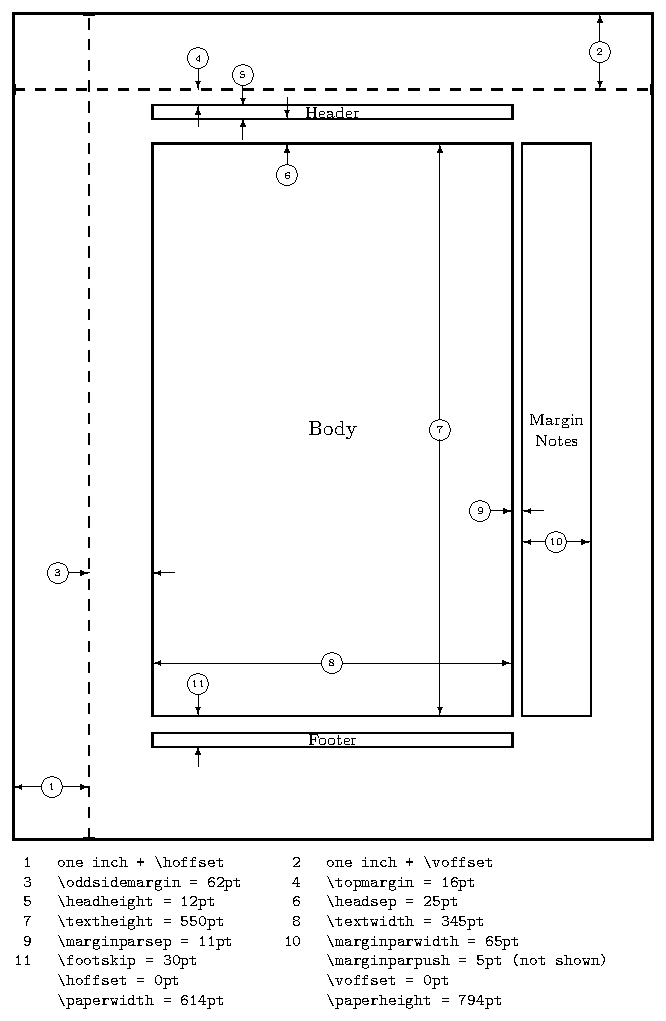
\includegraphics{layout-r}
   \end{center}
\end{quote}

這裡所謂的紙張大小\index{紙張大小},指的是 {\ttfamily paperwidth}\index{paperwidth} 和 {\ttfamily paperheight}\index{paperheight} 所圍成的範圍,並非實際上手上拿到的紙張大小,實際在手上的紙張通常會略大於我們這裡的所謂紙張,所以,正式列印時,還需做微調或截切才會是真正的這裡所謂的紙張大小(版面大小\index{版面大小})。

這是 10pt 內文大小,如果不指定紙張的話,\LaTeX{} 預設會使用美式 {\ttfamily letterpaper}\index{letterpaper} 的大小,如要使用歐、日式的 {\ttfamily a4paper}\index{a4paper} 的話,要另行指定。我們可以稍微看一下 \LaTeX{} 預設是如何安排版面空間的。其中 Header(頁眉)、Footer(頁足)及邊註的空間是不含括在內文 Body 裡頭的,這裡是只是單面的圖,如果是雙面的話,那偶數頁和奇數頁的邊註是要左右對換的,也就是說這個圖是奇數頁,偶數頁的話,邊註是在左邊。

這裡我們來看一下這些值所代表的意義:

\begin{quote}
   \begin{tabular}{ll}
      指令(值)              & 意義                         \\
      \hline
      \verb=\paperwidth=  & 紙張的寬度                   \\
      \verb=\paperheight=  & 紙張的高度                   \\
      \verb=\textwidth=  & 內文(body)的寬度           \\
      \verb=\textheight= & 內文(body)的高度           \\
      \verb=\headheight= & 頁眉(header)長度           \\
      \verb=\headsep= & 頁眉與內文間的距離           \\
      \verb=\footskip= & 內文底至頁足底之距離         \\
      \verb=\topmargin= & 頁眉上方的空白               \\
      \verb=\marginparwidth= & 邊註的寬度                   \\
      \verb=\marginparsep= & 邊註與內文的距離             \\
      \verb=\marginparpush= & 兩邊註間距                   \\
      \verb=\oddsidemargin= & 內文左邊的空白大小           \\
      \verb=\hoffset= & 微調版面在實際紙張的左右位置 \\
      \verb=\voffset= & 微調版面在實際紙張的上下位置 \\
      \index{paperwidth@\verb=\paperwidth=}\index{paperheight@\verb=\paperheight=}%
      \index{textwidth@\verb=\textwidth=}\index{textheight@\verb=\textheight=}%
      \index{headheight@\verb=\headheight=}\index{headsep@\verb=\headsep=}%
      \index{footskip@\verb=\footskip=}\index{topmargin@\verb=\topmargin=}%
      \index{marginparwidth@\verb=\marginparwidth=}\index{marginparsep@\verb=\marginparsep=}%
      \index{marginparpush@\verb=\marginparpush=}%
      \index{oddsidemargin@\verb=\oddsidemargin=}%
      \index{hoffset@\verb=\hoffset=}\index{voffset@\verb=\voffset=}%
   \end{tabular}
\end{quote}

\verb|\hoffset| 及 \verb|\voffset| 就是在調整版面在實際紙張上的正確位置,這樣印出來的時候才會在實際紙張的中央。

頭昏了嗎?這很正常,因為 \LaTeX{} 的版面設定對初接觸的人來說,是惡名昭彰的困難、麻煩,因此這裡不多談他的設定,剛開始實在沒有必要把時間花在這個地方。如果實際想調整版面,建議使用 {\sffamily geometry}\index{geometry@\textsf{geometry}} package。舉個例子,想讓各邊緣是 2cm 就好,那只要在 preamble\index{preamble} 區設定:

\begin{quote}
   \begin{verbatim}
\usepackage[margin=2cm]{geometry}
\end{verbatim}
\end{quote}

就可以了,如果以 12pt 大小的字,{\ttfamily a4paper} 紙張大小的設定的話,以中文而言,大約是每行 40 個中文字,這是內文的寬度。可以視情形自行調整 {\ttfamily margin}\index{margin} 的值就行了。我們很希望,下一版的 \LaTeX{} 能對這方面做改善,以方便使用者設定。
%更精確、詳細的設定方法,我們留到後面說明書籍成書時再來談,這樣就不致影響我們學習的正常進度。

\subsection{紙張大小}

\begin{quote}
   \begin{tabular}{>{\ttfamily}ll>{\ttfamily }ll}
      紙張    & 大小      & 紙張           & 大小        \\
      \hline
      a4paper & 21x29.7cm & letterpaper    & 8.5x11in    \\
      a5paper & 14.8x21cm & legalpaper     & 8.5x14in    \\
      b5paper & 17.6x25cm & executivepaper & 7.25x10.5in \\
   \end{tabular}
\end{quote}

至於如何指定紙張大小,這裡先簡單說明一下這篇文章的設定,談到 \LaTeX{} 的文稿類別時會再詳細說明。

\begin{quote}
   \begin{verbatim}
% 本文的設類別設定
\documentclass[12pt,a4paper]{report}
\end{verbatim}
\end{quote}

所以,這篇文章使用的是 {\ttfamily a4paper},內文字型的大小是 12pt。方括號的參數是選項,可以省略,如果省略的話,預設值就是 10pt/{\ttfamily letterpaper}。

\section{調整橫向空間}

這裡的橫向空間,例如 \verb|~|\index{~@\verb=~=} 這單字間正常空白,及 \verb|\quad| 這個 em\index{em} 寬度空白,都是在調整橫向的空白。但如果是要更大、或更小的空白時該如何調整呢?底下我們就來看看 \LaTeX{} 中有什麼控制指令可以運用:

\subsection{調整橫向空間的指令}

\begin{quote}
   \begin{tabular}{ll}
      指令                    & 意義                                                    \\
      \hline
      \verb=\hspace{單位}= & 向右空出某個度量單位的空白,如果是負數,則是向左        \\
      \verb=\hfill= & 讓左右兩旁的文字往兩邊擴張至一個行寬為止                \\
      \verb=\quad= & 空出一個 em 單位的空白                                  \\
      \verb=\qquad= & 空出二個 em 單位的空白                                  \\
      \verb=\thinspace= & 空出 $1/12$ 個 em 單位的空白                            \\
      \verb=\enspace= & 空出 $1/2$ 個 em 單位的空白                             \\
      \verb=\dotfill= & 作用和 \verb|\hfill| 相同,只是空白變成點     \\
      \verb=\hrulefill= & 作用和 \verb|\hfill| 相同,只是空白變成一橫線 \\
      \verb=\centering= & 此指令以後的文字將會居中排列,左右沿將不切齊            \\
      \verb=\raggedright= & 此指令以後的文字將會居左排列,右沿將不切齊              \\
      \verb=\raggedleft= & 此指令以後的文字將會居右排列,左沿將不切齊              \\
      \verb=\centerline{}= & 將大括號內的文字居中排列
   \end{tabular}
\end{quote}
\index{hspace@\verb=\hspace=}\index{hfill@\verb=\hfill=}%
\index{quad@\verb=\quad=}\index{qquad@\verb=\qquad=}%
\index{thinspace@\verb=\thinspace=}\index{enspace@\verb=\enspace=}%
\index{dotfill@\verb=\dotfill=}\index{hrulefill@\verb=\hrulefill=}%
\index{centering@\verb=\centering=}\index{raggedright@\verb=\raggedright=}%
\index{raggedleft@\verb=\raggedleft=}\index{centerline@\verb=\centerline{}=}

一行的行首使用 \verb|\hspace{單位}| 時將會失效,這時可以加個星號,例如 \verb|\hspace*{3em}|。

在使用 \verb|\centerline{}| 的場合,對於短文句很方便,因為他不會影響以下的文字,但他也不會折行,甚至加入換行符號也無效。所以如果文句長度超過一行的行寬,他會超出邊界,甚至就首尾的文字就看不到了。

其中 \verb|\thinspace| 又可以使用簡化的 \verb|\,| 來代替,主要是用在引號中又有引號的情形,通常這種情形,兩引號之間要有個間隔,以便區分,例如:

\begin{quote}
   \begin{verbatim}
``\,`Superman', he said.''
\end{verbatim}
\end{quote}

表現出來會是:

\begin{quote}
   ``\,`Superman', he said.''
\end{quote}

這樣才能區分出不同引號,否則會變成一個連三個 grave accent\index{grave accent} 的引號。請注意,由於這個指令是由非字母符號構成,所以,他的作用範圍在遇到符號本身後就結束了,後面不必空白或以大括號來限制其作用範圍,就好像曾提到過的 \verb|\@| 一樣的情形。

\subsection{調整橫向空間的環境}

\begin{quote}
   \begin{tabular}{ll}
      \verb|\begin{center}...\end{center}| & 讓這個環境內的內容置中               \\
      \verb|\begin{flushleft}...\end{flushleft}| & 讓這個環境內的內容靠左               \\
      \verb|\begin{flushright}...\end{flushright}| & 讓這個環境內的內容靠右               \\
      \verb|\begin{raggedright}...\end{raggedright}| & 讓這個環境內的內容靠左,右沿將不切齊 \\
      \verb|\begin{raggedleft}...\end{raggedleft}| & 讓這個環境內的內容靠右,左沿將不切齊 \\
   \end{tabular}
\end{quote}
\index{center@\texttt{center}}\index{flushleft@\texttt{flushleft}}%
\index{flushright@\texttt{flushright}}\index{raggedright@\texttt{raggedright}}%
\index{raggedleft@\texttt{raggedleft}}

進入環境,和上一節提到的指令,兩者有什麼不同呢?最大的不同是,這可以方便的指定一個範圍的文句讓他作用,而不會影響環境以外的文句。其次,進入環境,縱使和上下行連在一起,沒有空出空白行,他也會自動的在上、下行空出個空白行出來,使用指令的話則不會。

咦!這裡怎麼又有個 {\ttfamily raggedright} 及 {\ttfamily raggedleft}?原來他也是可以當環境來使用。由於這兩個指令會使以下的內容的左、右沿不切齊,因此使用上要非常小心,除非本來就想讓內文的左、右沿不切齊,否則,最好是使用有範圍限制的方式。當然,如果這兩個指令是用在某個其他環境範圍內,他的作用也將僅限於這個環境內,不會影響這個環境外的文句。

\subsection{引文環境}
\index{引文環境}

引文通常就是引用他人的文句,在引文的段落,兩旁都會出現內縮的情形,以便和正文相區隔,這也是一種空間的配置,可增加文章的易讀性。在 \LaTeX{} 裡頭有三種引文環境:{\ttfamily quote}, {\ttfamily quotation}, {\ttfamily verse}。這三者看起來很像,但有些微的差異。

\begin{quote}
   \begin{tabular}{>{\ttfamily }lll}
      環境      & 適用時機         & 特性                                     \\
      \hline
      quote     & 較短的短引文     & 每個段落第一行不內縮                     \\
      quotation & 多個段落的長引文 & 每個段落第一行會內縮                     \\
      verse     & 詩歌、詞引文     & 每個段落的第一行不內縮,但第二行起會內縮 \\
   \end{tabular}
\end{quote}
\index{quote@\texttt{quote}}\index{quotation@\texttt{quotation}}%
\index{verse@\texttt{verse}}

在 {\ttfamily verse} 的情形,通常會使用 \verb=\\=\index{\\@\verb=\\=} 來換行以便控制每一行的寬度。而且段落間距\index{段落間距}將不受外在設定的影響,其中 {\ttfamily quote} 和 {\ttfamily verse} 環境會預插入適當的段落間距,而 {\ttfamily quotation} 環境則不會。

底下我們來看看調整橫向空間的一個綜合實例:

\begin{quote}
   \begin{verbatim}
% example11.tex
\documentclass{article}
\usepackage{CJK}
\begin{document}
\begin{CJK}{Bg5}{hwmm}
\section{hspace}
\hspace*{2em}這是一個橫向空間調整的測試。\\
這是一個\hspace{2em}橫向空間調整的測試。\\
這是一個 \hspace{2em} 橫向空間調整的測試。
\section{hfill}
這是一個\hfill{}橫向空間調整的測試。
\section{quad}
這是一個\quad{}橫向空間調整的測試。\\
這是一個 \quad{} 橫向空間調整的測試。\\
這是一個\qquad{}橫向空間調整的測試。
\section{dotfill}
這是一個\dotfill{}橫向空間調整的測試。\\
這是一個 \dotfill{} 橫向空間調整的測試。
\section{hrulefill}
這是一個\hrulefill{}橫向空間調整的測試。
\section{center}
\begin{center}
這是一個橫向空間調整的測試。
\end{center}
\section{flushleft}
\begin{flushleft}
這是一個橫向空間調整的測試。
\end{flushleft}
\section{flushright}
\begin{flushright}
這是一個橫向空間調整的測試。
\end{flushright}
\section{quote}
這是節錄自伊索寓言的節錄故事:
\begin{quote}
An antwent to the bank of a river to quench its thirst, and
being carried away by the rush of the stream, was on the
point of drowning.
A Dove sitting on a tree overhanging the water plucked a
leaf and let it fall into the stream close to her. The Ant
climbed onto it and floated in safety to the bank.
\end{quote}
\section{quotation}
這是節錄自伊索寓言的節錄故事:
\begin{quotation}
An antwent to the bank of a river to quench its thirst, and
being carried away by the rush of the stream, was on the
point of drowning.
A Dove sitting on a tree overhanging the water plucked a
leaf and let it fall into the stream close to her. The Ant
climbed onto it and floated in safety to the bank.
\end{quotation}
\section{verse}
這是節錄自伊索寓言的節錄故事,這是節錄自伊索寓言的節錄故事,%
這是節錄自伊索寓言的節錄故事,這是節錄自伊索寓言的節錄故事:
\begin{verse}
An antwent to the bank of a river to quench its thirst, and
being carried away by the rush of the stream, was on the
point of drowning.
A Dove sitting on a tree overhanging the water plucked a
leaf and let it fall into the stream close to her. The Ant
climbed onto it and floated in safety to the bank.
\end{verse}
\section{centering}
\centering
這是一個橫向空間調整的測試。\\ % 這裡要換行,否則會是 \raggedright 的作用
\raggedright
\section{centerline}
\centerline{這是一個橫向空間調整的測試。}
\section{raggedright}
\raggedright
這是一個橫向空間調整的測試。
\section{raggedleft}
\raggedleft
這是一個橫向空間調整的測試。
\end{CJK}
\end{document}
\end{verbatim}
\end{quote}

編譯好的結果如下:

\begin{quote}
   \url{http://edt1023.sayya.org/tex/latex123/example11.tex}\\
   \url{http://edt1023.sayya.org/tex/latex123/example11.pdf}
\end{quote}

要注意是指令前後的空白,像 \verb|\hspace|, \verb|\dotfill|, \verb|\hrulell| 這類指令,指令前後空白都會算進去的。\verb|\quad|, \verb|\qquad| 這類指令,則後面的空白也是會算入的。另外,由例子中可以看出來,一個 em\index{em} 的寬度,大約是一個中文字的寬度,所以,我們預設使用 10pt 的字,這個 em 寬度就相當於 10pt 的寬度,所以,我們在第一行插入了 2em 寬度的空白,也就好像是內縮了兩個中文字一樣。

\section{調整縱向空間}

\begin{quote}
   \begin{tabular}{ll}
      \verb=\vspace{單位}=      & 向下空出某個單位的空白(行),負數則是向上                      \\
      \verb=\bigskip=      & 產生 12pt(11--12pt)的垂直空白(行)                           \\
      \verb=\medskip=      & 產生 6pt(5--7pt)的垂直空白(行)                              \\
      \verb=\smallskip=      & 產生 3pt(2--4pt)的垂直空白(行)                              \\
      \verb=\vfill=      & 和 \verb|\hfill| 類似,作用是將某段落向上頂,或往下擠 \\
      \verb=\parskip=單位= & 調整全文每個段落間的距離為某個單位
      \index{vspace@\verb=\vspace=}\index{bigskip@\verb=\bigskip=}%
      \index{medskip@\verb=\smallskip=}\index{vfill@\verb=\vfill=}%
      \index{parskip@\verb=\parskip=}
   \end{tabular}
\end{quote}

其中的 \verb|\bigskip, \medskip, \smallskip| 並非固定的,他們會視上下文脈絡的需要自動做微調,以達到一整頁較一致的空間配置。\verb|\vspace| 如果是出現在一頁的第一行或最後一行時,將會失去作用,這時可以加個星號,\verb=\vspace*{單位}=\index{vspace@\verb=\vspace*=}。

為了維持版面的一致性\index{版面一致性},使用縱向空間調整的指令時要特別留意,例如章節標題上下的空間、各段落間的空間,進入環境前後所空出的空間,這都有一個固定值,\LaTeX{} 會自動去調整,不必由使用者自行動手,除非是封面這種單獨頁。所以,使用縱向空間調整指令時,要非常注意整體的一致性,這也是排版上的一個很重要的原則。

這裡舉這篇文章的內頁封面\index{內頁封面}為例來綜合說明,橫、縱向空間的運用。還記得第 \ref{sec:titlepage} 節的 title page\index{title page} 的指令嗎?其實我們也可以自行設計一個獨立的內頁封面,使用的是 \LaTeX{} 本身的 {\ttfamily titlepage}\index{titlepage@\texttt{titlepage}} 環境。這裡的圖檔引用是我們還沒有學習到的,沒關係,只要大原則抓住就行了。

\begin{quote}
   \begin{verbatim}
% example12.tex
\documentclass[12pt,a4paper]{report}
\usepackage{CJK}     % 引入所需要的 packages
\usepackage{graphicx}
\begin{document}
\begin{CJK}{Bg5}{hwmm}
\begin{titlepage}    % 使用 titlepage 環境
\vspace*{5ex}
  \begin{flushright} % 大標題靠右
    \Huge\textbf{大家來學 \LaTeX}
  \end{flushright}
  \rule{\textwidth}{.256ex}
  \begin{flushleft}  % 版本號碼及日期靠左,和大標題之間以一橫線隔開
    Version 0.1 draft\\
    \today
  \end{flushleft}    % 圖檔位於中央偏左
  \vspace{8ex}       % 空出 8ex 的垂直空間
  \hspace{2em}\includegraphics[scale=.75]{cover2.1} % 引入圖檔,並將這個
  \vspace{8ex}                                      % 圖檔橫向右移 2em
  \begin{flushright} % 作者資訊靠右
    By Edward G.J. Lee 李果正\\
    Email:\texttt{edt1023@info.sayya.org}
  \end{flushright}
\end{titlepage}
\end{CJK}
\end{document}
\end{verbatim}
\end{quote}

由於配合版面的問題,其中有一些數據有更動,而且也省略了一些我們還沒有學習到的 packages,但大結構則和原始文稿一樣。所以,和這篇文章的 PDF 格式比較會發現,大標題的字體小了一點,而且沒有顏色,也沒有超連結\index{超連結}。

使用 {\ttfamily titlepage}\index{titlepage@\texttt{titlepage}} 環境後,在 {\ttfamily report/book}\index{report@\texttt{report}}\index{book@\texttt{book}} 文稿他會自成一沒有頁數的單獨頁,在 {\ttfamily article}\index{article@\texttt{article}} 類別,因為會和內文連接,所以,在選項的部份要多加一個 {\ttfamily titlepage}\index{titlepage} 的選項。另外,在 {\ttfamily titlepage} 裡頭就不能再使用 \verb|\title|\index{title@\verb=\title=}, \verb=\author=\index{author@\verb=\author=} 指令了,在本文的地方也不必再下 \verb=\maketitle=\index{maketitle@\verb=\maketitle=} 指令。

編譯好的例子如下:

\begin{quote}
   \url{http://edt1023.sayya.org/tex/latex123/example12.tex}\\
   \url{http://edt1023.sayya.org/tex/latex123/example12.pdf}
\end{quote}

這裡要特別說明的是,引入圖檔要使用 \textsf{graphicx}\index{graphicx@\textsf{graphicx}} package(這是最常用的,也有其他的方法來引用),引入的指令是 \verb=\includegraphics=\index{includegraphics@\verb=\includegraphics=},這個我們會在第 \ref{ch:graphic} 章會討論,在這裡我們把圖檔縮小成為原圖的 {\ttfamily 75\%},否則整個封面會超出一頁。這個圖檔是由 \MP\index{metapost@\MP} 檔案所編譯而來的,他是一種 eps 圖檔\index{eps 圖檔}(簡單的說,是含有邊界數據去除不必要周圍空白的 ps 檔\index{ps 檔},方便引入或輸出至文稿中),編譯的方法如下:

\begin{quote}
   \begin{verbatim}
mpost cover2.mp
\end{verbatim}
\end{quote}

這樣就會產生 {\ttfamily cover2.1} 這個 eps 圖檔,這樣就可以直接引入了。他的原始碼及 eps 圖檔在:

\begin{quote}
   \url{http://edt1023.sayya.org/tex/latex123/cover2.mp}\\
   \url{http://edt1023.sayya.org/tex/latex123/cover2.1}
\end{quote}


\section{條列環境}

條列環境\index{條列環境}也是屬於一種空間的控制,他把一些文字按一定的方式來排列,條列環境中一些起頭的符號、文數字或字串,我們稱之為項目標籤(item label)\index{項目標籤(item label)},利用這些不一樣的排列位置及不一樣的項目標籤起頭來敘述文句,就可以達到醒目的作用。這是以章節分隔以外,相當常用讓內容一目了然的方法,建議多多利用。請千萬記得,環境中還可以有環境,而且以下三種的條列方式可以混合交叉使用。

\subsection{項目式條列環境(itemize)}
\index{項目式條列環境(itemize)}

這是以符號來起頭醒目的一種條列方式。例如:

\begin{quote}
   \begin{verbatim}
\begin{itemize}
\item 第一大項,這裡是第一大項。
\item 第二大項,這裡是第二大項。
 \begin{itemize}
 \item 第一小項,這裡是第一小項。
 \item 第二小項,這裡是第二小項。
 \end{itemize}
\item 第三大項,這裡是第三大項。
\item 第四大項,這裡是第四大項。
\end{itemize}
\end{verbatim}
\end{quote}

排版出來會變成:

\begin{quote}
   \begin{itemize}
      \item 第一大項,這裡是第一大項。
      \item 第二大項,這裡是第二大項。
            \begin{itemize}
               \item 第一小項,這裡是第一小項。
               \item 第二小項,這裡是第二小項。
            \end{itemize}
      \item 第三大項,這裡是第三大項。
      \item 第四大項,這裡是第四大項。
   \end{itemize}
\end{quote}

\subsection{列舉式條列環境(enumerate)}
\label{subsec:enume}\index{列舉式條列環境(enumerate)}

這是以數目字或字母或羅馬數字來起頭醒目的條列方式。同樣的例子,改成 {\ttfamily enumerate} 的話,會排版成:

\begin{quote}
   \begin{enumerate}
      \item 第一大項,這裡是第一大項。
      \item 第二大項,這裡是第二大項。
            \begin{enumerate}
               \item 第一小項,這裡是第一小項。
               \item 第二小項,這裡是第二小項。
            \end{enumerate}
      \item 第三大項,這裡是第三大項。
      \item 第四大項,這裡是第四大項。
   \end{enumerate}
\end{quote}

\subsection{敘述式條列環境(description)}
\index{敘述式條列環境(description)}

這是以一個簡短文字敘述來起頭醒目的條列方式。再把他改成 {\ttfamily description} 的話,他是以粗體文字來起頭醒目的,這些文字要用方括號括住。

\begin{quote}
   \begin{verbatim}
\begin{description}
\item[第一大項] 這裡是第一大項。
\item[第二大項] 這裡是第二大項。
  \begin{description}
  \item[第一小項] 這裡是第一小項。
  \item[第二小項] 這裡是第二小項。
  \end{description}
\item[第三大項] 這裡是第三大項。
\item[第四大項] 這裡是第四大項。
\end{description}
\end{verbatim}
\end{quote}

排版出來的結果是:

\begin{quote}
   \begin{description}
      \item[第一大項] 這裡是第一大項。
      \item[第二大項] 這裡是第二大項。
            \begin{description}
               \item[第一小項] 這裡是第一小項。
               \item[第二小項] 這裡是第二小項。
            \end{description}
      \item[第三大項] 這裡是第三大項。
      \item[第四大項] 這裡是第四大項。
   \end{description}
\end{quote}

要注意的是,不管哪一種的條列環境,每個項目(item)的文字敘述會自動折行,這相當方便,使用者只要把條列的結構弄妥,專心打每個項目的內容就成了。而且,如果使用方括號括住一些字元、字串或符號,那帶頭的標示將會是這些字元、字串或符號,如果是列舉式的條列方式,那麼有方括號的將不被編號,會自動跳過,編號順序則會自動順延。

%\section{enumerate 巨集套件}

%\subsection{條列環境內的空間控制}


\section{線框}
\index{線框}

線框在排版上佔有一定的地位,因為他可以區隔不同的空間,也可以讓某些部份突顯出來。但是,過多的線框也是會有喧賓奪主的不好副作用,使用上可能要適可而止。這裡我們要談的是單純的線框,表格\index{表格}也是線框的一種應用,我們將會在第 \ref{ch:graphic} 章,再來談表格的處理。

%在 \LaTeX{} 的線框可分為三種:LR、Rule 及 Par。

%\begin{quote}
%\begin{tabular}
%線框種類 & 意義 \\
%\hline
%LR  & left-right,線框及線框中的內容由左至右 \\
%Rule & 
%Par
%\end{tabular}
%\end{quote}

\subsection{直線(rule)}
\index{直線(rule)}

直線也是屬於方框的一種,就是一個實體長方形,只不過,他的高或寬(線的組細)只有一點點,所以,看起來就一像直線罷了。

\begin{quote}
   \begin{verbatim}
\rule[上下位置(單位)]{寬}{高}
\end{verbatim}
\end{quote}

寬及高應不必多做解釋,那個上下位置是什麼呢?這個上下位置是和基線(baseline)\index{基線}\index{baseline}在比較的,如果沒有指定,那就是在基線的位置,如果有指定,就依正負值調整和基線的相對位置,正值由基線向上調整,負值則由基線向下調整。這裡來看個個實例就瞭解了:

\begin{quote}
   \begin{verbatim}
% example13.tex
\documentclass{article}
\parskip=3pt
\parindent=0pt
\begin{document}
This is a line.       % 畫高 1pt 寬 3cm 的橫線。
\rule{3cm}{1pt}
\rule[1ex]{3cm}{1pt}
\rule[-1ex]{3cm}{1pt}
\rule{1pt}{3cm}      % 畫高 3cm 寬 1pt 的直線。
\rule{3cm}{0pt}TEST. % 把 TEST 向右推 3cm。
\rule{2cm}{3cm}      % 畫高 3cm 寬 2cm 的實體方框。
\textcolor{blue}{This is color lines.}
\textcolor{red}{\rule{3cm}{1pt}}        % 有顏色的線框。
\textcolor{green}{\rule[1ex]{3cm}{1pt}}
\textcolor{blue}{\rule[-1ex]{3cm}{1pt}}
\end{document}
\end{verbatim}
\end{quote}

編譯好的例子在:

\begin{quote}
   \url{http://edt1023.sayya.org/tex/latex123/example13.tex}\\
   \url{http://edt1023.sayya.org/tex/latex123/example13.pdf}
\end{quote}

由例子中可以看得出來,這個畫線指令並不是單單縱、橫畫線而已,靈活運用的話,可以做出許多不同的效果,例如方條圖之類的。

\subsection{文字底線(underline)}
\index{文字底線(underline)}

有時候我們希望在書寫文字的同時,也在其下畫線。\LaTeX{} 有現成的指令可以使用,那就是 \verb|\underline{文字}|\index{underline@\verb=\underline=},會在文字底線的部份同時畫上線條。當然,使用上常常會和現在的橫線搞混,因此使用時要特別留意整個頁面上是否已經存在了許多橫線。

\subsection{方框(box)}
\index{box}

這裡主要指的文字方框,繪圖上的一般框形在第 \ref{ch:graphic} 章時再來討論。這一章的開頭就已談到,整篇文章是由一個個的 box 所構成的,這裡的方框則是一個典型的 box,他的地位,當然是和前面所說的 box 一樣,\TeX/\LaTeX{} 會把他視為一個單一的字母來處理。

我們先來看看最簡單的方框的指令:

\begin{quote}
   \begin{tabular}{ll}
      指令                     & 意義及作用                                         \\
      \hline
      \verb=\frame{文字}= & 將文字內容以可見的方框框住,方框和文字間沒有間距   \\
      \verb=\fbox{文字}= & 將文字內容以可見的方框框住,方框和文字間有一定間距 \\
      \verb=\mbox{文字}= & 作用和 \verb|\fbox| 同,但方框不可見
   \end{tabular}
\end{quote}
\index{frame@\verb=\frame=}\index{fbox@\verb=\fbox=}%
\index{mbox@\verb=\mbox=}

以上的指令都可以形成方框文字。

方框也有可以調整的指令:

\begin{quote}
   \begin{tabular}{ll}
      指令                     & 意義及作用                                             \\
      \hline
      \verb|\framebox[寬度][對齊方式]{文字}| & 與 \verb|\fbox| 同,但可指定寬度及對齊方式 \\
      \verb|\makebox[寬度][對齊方式]{文字}| & 與 \verb|\mbox| 同,但可指定寬度及對齊方式
      \index{framebox@\verb=\framebox=}\index{makebox@\verb=\makebox=}
   \end{tabular}
\end{quote}

這裡的寬度指的是方框的寬度,不指定的話,作用就如同 \verb|\fbox| 及 \verb|\mbox| 一樣,以包住整個文字範圍為寬度,由於我們不容易測知文字內容的寬度有多少,因此寬度的指定可以使用下列相對單位的方式:

\begin{quote}
   \begin{tabular}{ll}
      寬度                     & 作用                                                             \\
      \hline
      \verb|\width| & 這個寬度就是 \verb|\fbox| 圍住時的方框寬度           \\
      \verb|\height| & 這是正常基線至框頂的高度                                         \\
      \verb|\depth| & 這是正常基線至框底的高度                                         \\
      \verb|\totalheight| & 這是 \verb|\height| 和 \verb|\depth| 之總和 \\
   \end{tabular}
\end{quote}

例如,我們指定 \verb|2\width| 他的意思就是以 \verb|\fbox| 包住此文字內容時,其方框寬度的二倍寬。參數裡頭的對齊方式,可有下列幾種:

\begin{quote}
   \begin{tabular}{>{\ttfamily }ll}
      對齊方式 & 作用                                 \\
      \hline
      c        & center,文字位於方框中央,這是預設值 \\
      l        & flushleft,文字位於方框左方          \\
      r        & ushright,文字位於方框右方           \\
      s        & stretch,文字平均分分布於方框中
   \end{tabular}
\end{quote}

不指定的話,當然就是位於方框中央位置了。我們也可以指定可見方框的線的粗細,及方框和文字間的間隔距離:

\begin{quote}
   \begin{tabular}{ll}
      指令                     & 作用                 \\
      \hline
      \verb|\fboxrule=單位| & 指定方框線條粗細     \\
      \verb|\fboxsep=單位| & 指定文字和框緣的間距 %
      \index{fboxrule@\verb=\fboxrule=}\index{fboxsep@\verb=\fboxsep=}%
   \end{tabular}
\end{quote}

請注意,這不會影響 \verb|\frame{}|。如果想特別的置放方框的位置,也可以使用 \verb|\raisebox|\index{raisebox@\verb=raisebox=} 指令:

\begin{quote}
   \begin{verbatim}
\raisebox{上下位置(單位)}[深度][高度]{文字內容}
\end{verbatim}
\end{quote}

這裡的上下位置的意義和 \verb|\rule| 指令裡頭的一樣,只不過,這裡的上下位置一定要指定,沒有預設值,不指定會編譯錯誤。請千萬記得,方框中當然是還可以有方框的。我們現在就來看一個綜合的實例:

\begin{quote}
   \begin{verbatim}
% example14.tex
\documentclass{article}
\parskip=3ex
\parindent=0pt
\begin{document}
\frame{This is frame.}
\mbox{This is mbox.}
\fbox{This is fbox.}
\framebox{This is a framebox with no argumant.}
\framebox[1.5\width]{This is a framebox.}
\framebox[1.5\width][l]{This is a framebox with \texttt{l}.}
\framebox[1.5\width][r]{This is a framebox with \texttt{r}.}
\framebox[1.5\width][s]{This is a framebox with \texttt{s}.}
This is baseline.
\raisebox{3ex}[5\height]{This is a raisebox which lift 3ex.}
This is baseline.
\fbox{\raisebox{-3ex}[5\height]{This is a raisebox which lift $-$3ex.}}
\fboxrule=1.5pt
\fboxsep=8pt
\framebox[1.5\width][s]{This is a framebox with \texttt{s}.}
\end{document}
\end{verbatim}
\end{quote}

這應無需多加解釋,編譯好的例子在:

\begin{quote}
   \url{http://edt1023.sayya.org/tex/latex123/example14.tex}\\
   \url{http://edt1023.sayya.org/tex/latex123/example14.pdf}
\end{quote}

\subsection{段落方框}
\index{段落方框}

另外,也有用於段落文字的方框,可以控制某個段落出現在某特定的空間、位置。我們常常把這種安排稱為迷你版面,把版面內容置於一個不可見的方框當中,當然,這個方框和一般的 box,例如字母,仍然處於同樣的地位,\LaTeX{} 會把他當成一個字母單位來處理。

\begin{quote}
   \begin{verbatim}
\parbox[對齊方式][高度][內文位置]{寬度}{文字內容}
\begin{minipage}[對齊方式][高度][內文位置]{寬度}
  段落內容
\end{minipage}
\end{verbatim}
\end{quote}
\index{parbox@\verb=parbox=}\index{minipage@\texttt{minipage}}

這裡的第一個選擇性參數「對齊方式」:

\begin{quote}
   \begin{tabular}{>{\ttfamily }ll}
      t & top,段落方框的上沿對齊一行的基線              \\
      b & bottom,段落方框的下沿對齊一行的基線           \\
      c & center,段落方框的中央對齊一行的基線,這是預設 \\
   \end{tabular}
\end{quote}

\verb|\parbox| 指令通常用於較短的文字內容,如果是較長的段落,那使用 {\ttfamily minipage} 環境會比較方便。這些段落方框和上面所談到的一些方框最大的不同是,段落方框本就是用來排版小段落文句,因此他會和一般正常文章段落一樣的處理,例如他會自動斷行,碰到空白行也會起新段落,但各段落預設是不縮排的,而且,在安排上會比一般的段落緊湊,一些邊緣的間距會縮減成 0pt。

高度不去指定的話,那就是以整個版面經斷行處理後,整個文字段落所形成的高度。至於內文位置指的也是 \texttt{t, b, c} 這些,意思是文字段落在方框內的上下位置,當然,這要有指定方框高度時才會有意義,因此,「內文位置」和「高度」是要同時指定的,要非常注意的是,如果指定了高度,但沒有指定內文位置,則預設是等於前面使用的「對齊方式」所指定的參數。

這些參數的使用會有些煩複,但這是彈性所帶來的「必要之惡」,不必去死記,只有在第一次接觸時把他搞清楚就夠了,實際要用到時再來查他的詳細參數,常用的指令、環境,大概多查幾次就自然而然的記起來了。
  % space.tex
% !TeX root = ../main.tex

\chapter{\LaTeX\ 的標準文稿類別}
\label{ch:class}\index{文稿類別}

這章主要是在說明 \LaTeX{} 文稿的類別(document class\index{document class})\footnote{這在舊的版本稱為 style,這兩個詞意義上差不多,這些都是 \TeX{} 延伸出來的巨集定義,專門用來定義文章的大結構,以便簡化使用上及文稿的內容。},這是 \LaTeX{} 規範文稿整體結構的方法。使用 class 的用意,就是把版面結構處理和實際文稿分開,這樣的最大好處就是維持整篇文章排版結構上的一致性,也使文稿內容更清爽簡潔,使用者只要專心於文稿內容的寫作即可,如果 class 定義的好,也可以達到一文多變化又不變更文稿內容的目的,只要把引用的 class 換成別的就可以了,其他的可以不必更動。

目前,\LaTeX{} 有五種標準類別用於一般文件,可用於一般的書信、雜誌、期刊、報告及論文。但有些期刊、論文會要求一定的結構,這時得依需求另行訂定。因此,也有其他的類別存在,標準類別並不是唯一的。甚至,也可以自行撰寫自己的文稿類別。當然,我們一般使用是不需要這麼講究,這裡只介紹 \LaTeX{} 的標準類別。而且,如果有和他人交換文稿的需求時,我們應該盡可能的使用流通性較廣泛的類別。

另外,也有一些是關於 \LaTeX{} 說明文件及 macro\index{macro} 寫作時要用到的類別,這些已超出本篇文章的範圍。

\section{\LaTeX{} 類別的宣告}
\index{類別的宣告}

\LaTeX{} 的類別,要在文稿的一開頭時就宣告(當然,其上有註解是沒有關係的),他的一般格式如下:

\begin{quote}
   \begin{verbatim}
\documentclass[選擇性參數]{類別}
\end{verbatim}
\end{quote}
\index{documentclass@\verb=\documentclass=}

選擇性參數是可以省略的,但類別名稱則不能省,一定要指定一個類別。而且只能只有一個類別。

\section{類別的選擇性參數}

選擇性參數可以選擇多個,各個選項是以逗點分開的。

\begin{enumerate}
   \item {\ttfamily 10pt, 11pt, 12pt}\\
         指定內文一般正常字的大小,預設是 {\ttfamily 10pt}。其他點數沒有外來 package 的幫忙不能指定。
   \item {\ttfamily a4paper, letterpaper, b5paper, executivepaper, legalpaper}\\
         指定紙張大小,預設是 {\ttfamily letterpaper}。
   \item {\ttfamily fleqn} \\
         使數學式靠左對齊,預設是居中對齊。\index{fleqn@\texttt{fleqn}}
   \item {\ttfamily leqno} \\
         使數學式編號靠左,預設是靠右。
   \item {\ttfamily titlepage, notitlepage}\index{titlepage@\texttt{titlepage}}\index{notitlepage@\texttt{notitlepage}} \\
         決定 title page 是否獨佔一頁。預設 \texttt{article}\index{article@\texttt{article}} 不獨佔一頁,但 \texttt{report/book}\index{book@\texttt{book}}\index{report@\texttt{report}} 則會獨佔一頁,在這裡是可以指定來變更預設行為,例如 \texttt{article} 文稿,指定 \texttt{titlepage} 的話,那 title page 就會獨佔一頁。
   \item {\ttfamily onecolumn, twocolumn} \\
         文章單欄或兩欄式,預設是單欄,也就是不分欄。\index{onecolumn@\texttt{onecolumn}}\index{twocolumn@\texttt{twocolumn}}
   \item {\ttfamily twoside, oneside}\index{twoside@\texttt{twoside}}\index{oneside@\texttt{oneside}} \\
         是否區分奇偶數頁。預設 \texttt{article/report} 不區分,\texttt{book} 則會區分。一般的書籍,在裝訂的部份,他的中央線稱為書脊,偶數頁會在打開書籍時的左方,而且其中內容會偏向書脊的中央(此時是向右),反之,奇數頁會在右,內容一樣會偏左向書脊,在 \texttt{oneside} 的情形則不做這樣的區分,不管奇偶頁都會在紙張的中央部位。
   \item {\ttfamily landscape} \\
         橫向列印或縱向列印,預設縱向(portait)。\index{landscape@\texttt{landscape}}\index{portait@\texttt{portait}}
   \item {\ttfamily draft}\index{draft@\texttt{draft}} \\
         草稿式編譯,這時圖檔將不會被引入,可加快編譯的速度。不過,如果編譯是使用向量字型的話,編譯速度應該是還算很快。但使用 {\ttfamily draft} 的一個好處是,過長的地方會標示出來。
   \item {\ttfamily openright, openany}\index{openright@\texttt{openright}}\index{openany@\texttt{openany}} \\
         這是在控制,章的開始是否是奇數頁(right-hand page)\index{奇數頁(right-hand page)}。在 \texttt{book} 類別,預設章會從奇數頁開始,report 類別則不會。\texttt{article} 類別沒有章,所以,對此一設定會忽略。
\end{enumerate}

\section{類別的種類}

這裡只列出一般文章使用的類別,其他特殊巨集或 \LaTeX{} 正式文件所使用的類別就不列出了,一般使用,這些類別就足夠了。

\begin{quote}
   \begin{tabular}{>{\ttfamily }lll}
      類別    & 一般用途       & 特性                                           \\
      \hline
      article & 一般短文       & 無章,連續頁方式的安排,無奇偶數頁的區分       \\
      report  & 較長論文       & 章會起新頁,預設無奇偶數頁的區分               \\
      book    & 書籍類         & 章會於奇數頁起新頁,預設有偶數頁的區分         \\
      letter  & 信件           & 英文信件格式                                   \\
      slides  & 幻燈片         & 幾乎另用外來套件取代                           \\
      minimal & 測試及寫新類別 & 這是最簡單的類別,只規定了內文的寬、高,正常字
   \end{tabular}
\end{quote}
\index{article@\texttt{article}}\index{report@\texttt{report}}%
\index{book@\texttt{book}}\index{letter@\texttt{letter}}%
\index{slides@\texttt{slides}}\index{minimal@\texttt{minimal}}

當然,這些用途並不是固定不變的,得看使用者的安排,不想多花時間、精神的話,那就依 \LaTeX{} 預設的格式去使用,至少就不會太離譜。其中 \texttt{minimal} class 是用來測試用的,或者寫新的 class 用的,他完全沒有版面的安排,例如,沒有章節的結構,各種間距也沒有定義,預設的字型是正常字,沒有其他的變化,幾乎所有的變化要自行去定義。
  % class.tex
% !TeX root = ../main.tex

\chapter{巨集套件}
\label{ch:package}\index{巨集套件}

\LaTeX{} 系統已經好久沒有更新,有些部份可能會跟不上實際的腳步,而且有些內定的巨集定義,經過大家的使用,發覺並不是那麼的順手,尤其是功能的強化方面,因此這章談談如何引用他人已經寫好的巨集,這很重要,盡量避免重複製造輪子,寫 \TeX{}/\LaTeX{} macro\index{macro} 可說是很專業的工作,要避免破壞了整體的結構,所以先找看看有什麼巨集套件可以使用。

% %萬一找不到適合的巨集套件,或這些巨集套件的定義仍不符所需,這時我們就得自行修改定義,甚至是重新定義來符合所需,這也是這一章準備探討的一個主題。但是,不是每一個人都有充裕的時間去學習 \TeX/\LaTeX{} 的巨集語言,所以這裡探討的以實用、簡單的定義方法為主,稍微複雜的已不符合一般使用的原則,也和這篇文章的構想範圍不符。

\section{一般套件的使用}

我們曾在第 \ref{subsec:preamble} 小節,頁 \pageref{subsec:preamble},提到過簡單巨集的引用,事實上,有些巨集含有許多的參數來做微調,但是每個巨集套件的參數都不會一樣,因此,使用套件之前要先看一看他所附上的使用手冊。幾乎大部份的巨集套件都有使用手冊,如果是系統上就有的巨集,那麼這些文件通常會放在:

\begin{quote}
  \begin{verbatim}
$TEXMF/doc  => Unix-like 系統
$TEXMF\doc  => DOS/Windows 系統
\end{verbatim}
\end{quote}

這些目錄底下,這些文件會有原始 \TeX/\LaTeX{} 文稿,也有編譯好的 \texttt{*.dvi} 或 \textsc{PostScript}\index{PostScript@\textsc{PostScript}} 檔可以閱覽,為求方便的話,可以將他們轉成 pdf 格式來閱覽,原因是可以以關鍵字來搜尋全文,在查指令、環境時會比較方便。在 Unix-like\index{Unix-like} 系統或 Windows\index{Windows} 下的 cygwin\index{cygwin} 環境的話,可以使用 \texttt{texdoc}\index{texdoc@\texttt{texdoc}} 這個指令來閱覽,例如:

\begin{quote}
  \begin{verbatim}
texdoc amsguide  => 閱覽 amsguide.dvi 這個檔的說明
texdoc -s ams    => 查系統上所有含 ams 字樣的文件
\end{verbatim}
\end{quote}


\section{\LaTeX{} 官方文件中的標準巨集套件}

底下是 \LaTeX{} 官方文件中所附的標準巨集套件。雖然是標準巨集套件,但一般情形下,使用這些 packages 的機會並不多,都是有特殊需要時才會引入。

\subsection{alltt}\index{alltt@\textsf{alltt}}

這個巨集套件提供 \texttt{alltt}\index{alltt@\texttt{alltt}} 環境,和 \texttt{verbatim}\index{verbatim@\texttt{verbatim}} 環境的作用相同,只是 \textbackslash{},\{,\} 的作用和一般文章中相同會被 \LaTeX{} 解讀。這有什麼用呢?這樣一來 \LaTeX{} 這個特殊標誌也可以使用,也可以讓環境中的文字具有顏色,或做其他變化,當然,裡頭的文字預設仍然是使用打字機字族\index{打字機字族}的。

\subsection{doc}\index{doc@\textsf{doc}}

這是用來寫 \LaTeX{} 文件的巨集套件,這在使用 \texttt{ltxdoc}\index{ltxdoc@\texttt{ltxdoc}} 這個 class 的同時就會載入 \textsf{doc} package。由於這不是用於一般的文件使用場合,所以,這裡就不多談,有興趣的話可自行參考他的文件說明。

\subsection{exscale}\index{exscale@\textsf{exscale}}

由於原先的 Computer Modern font\index{Computer Modern font} 中的數學延伸符號(\texttt{cmex}\index{cmex@\texttt{cmex}})只有 10pt 大小的字型(\texttt{cmex10}),內文放大到 \texttt{large} 以上的字型時,例如放大到 \texttt{Large} 時,有些數學符號仍然會維持一定的大小,這時可以使用這個套件,讓這些數學符號也跟著放大,例如積分符號。\textsf{exscale} 只有字型縮放的定義,因此只要把這個套件在 preamble\index{preamble} 區引用就可以了,無需任何指令。

不過,這裡要說明一下,在 \TeX/\LaTeX{} 裡字型放大,有時可能會造成表現失真的情形,尤其是數學式子,為了顧及數學式子中各個字母間的空間安排,\texttt{cmex10} 的設計並不適合拿來放大,可以把 \texttt{cmr5} 放大成 10pt 和真正的 \texttt{cmr10} 來比較就會知道表現出來會不一樣,因此,如果考慮精確配合的問題,放大數學式子的字型時可能要考慮一下使用場合,尤其目前採用向量字更是如此。請試試以下的例子,我們把 \texttt{cmr5}、\texttt{cmr10} 及 \texttt{cmr12} 同樣放大到 30pt 來看看結果會不會一樣:

\begin{quote}
  \begin{verbatim}
% test-fonts.tex
\font\largecmr=cmr12 at 30pt
\largecmr
This is cmr12 at 30pt.
\font\largecmr=cmr10 at 30pt
\largecmr
This is cmr10 at 30pt.
\font\largecmr=cmr5 at 30pt
\largecmr
This is cmr5 at 30pt.
\bye
\end{verbatim}
\end{quote}

請注意,這是 \TeX\ 文稿,不是 \LaTeX{} 文稿,所以要使用 \texttt{tex}\index{tex@\texttt{tex}} 或 \texttt{pdftex}\index{pdftex@\texttt{pdftex}} 來編譯,他的結果如下,大家可很清楚的看得出來,雖然同樣是向量字,但放大時的表現並不會一樣:

\begin{quote}
  \url{http://edt1023.sayya.org/tex/latex123/test-fonts.tex}\\
  \url{http://edt1023.sayya.org/tex/latex123/test-fonts.pdf}
\end{quote}

根據 Knuth\index{Knuth} 教授當初設計 \MF\index{metafont@\MF},他的理念是一個同樣的字型在放大的時候,同一個字,他的筆劃置放的相對位置應該要隨放大的倍數而稍加調整。因此,假如我們只使用一種向量字型\index{向量字型},用在不同的放大倍率的時候,文字符號間的空間配合會產生不一樣的結果,尤其是用在數學式子\index{數學式子}的時候,更加明顯。

當然,實用上 \MF\ 雖然也是一種向量字型,但由於太過於複雜,不適合拿來螢幕顯示上用,所以才會退而求其次,轉成 pk 點陣字型來使用。這也就是為什麼同樣是 \texttt{cmr} 的字型,會有幾種不同點數的獨立字型的原因,縱使是向量字也是如此。\TeX\ 已經 20 幾歲了,但是,我們的字型技術似乎還是沒有完全趕上當初 Knuth 教授的理念。

\subsection{fontenc}\index{fontenc@\textsf{fontenc}}

在第 \ref{subsec:font-attr} 小節,頁 \pageref{subsec:font-attr},曾提到字型編碼的問題。要改變字型編碼,可以使用這個 \textsf{fontenc} package。以 T1 font encoding\index{T1} 來說:

\begin{quote}
  \begin{verbatim}
  ...
\usepackage[T1]{fontenc}
  ...
\end{verbatim}
\end{quote}

這樣就可以了,但由於一些字型,例如歐洲字元,在原來的 Computer modern Type1 字型中安排不一樣,所以,有些部份會使用原始的 \MF\ 字型所轉換成的 pk 點陣字,這樣的話,一般印表機印出來是差異不大,但如果是想製作成 PDF 格式在螢光幕閱覽的話,字型的表現會變得很醜。理想的話,要安裝 \texttt{cm-super}\index{cm-super@\texttt{cm-super}} Type1 字型,但是一般使用者恐怕自行安裝字型會有困難。這在 te\TeX\ 2.x\index{tetex@te\TeX} 以後的版本,已經有附上 \textsf{pxfonts}\index{pxfonts@\textsf{pxfonts}} 及 \textsf{txfonts}\index{txfonts@\textsf{txfonts}} package 及其字型,所以,如果是新近版本的 te\TeX\ 的話,可以由以下的方式來使用:

\begin{quote}
  \begin{verbatim}
  ...
\usepackage{txfonts}
\usepackage[T1]{fontenc}
  ...
\end{verbatim}
\end{quote}

其中 \textsf{txfonts} 是模擬 Times 系列的字型,\textsf{pxfonts} 是模擬 Palatino 系列的字型。當然,這裡關於字型的問題有點複雜,這不在這篇文章的討論範圍,只能做簡單的說明,如果沒有特殊需要,例如,歐洲字元、一些有重音符號的字母,那使用預設的 OT1 編碼就行了,因為這些套件所附的有些字型,只有一種大小的 Type1 字型在縮放,因此使用上恐怕會有失真\index{失真}的情形。

\subsection{graphpap}\index{graphpap@\textsf{graphpap}}

這是產生方格紙的巨集。他提供了一個指令,可以畫方格,可以配合 \texttt{picture}\index{picture@\texttt{picture}} 環境來使用,他的語法是:

\begin{quote}
  \begin{verbatim}
  ...
\usepackage{graphpap}
  ...
\graphpaper[n](x,y)(x1,y1)
  ...
\end{verbatim}
\end{quote}

其中的 \texttt{n} 如果省略的話,預設是 10,他指的是方格紙的最小刻度單位。\texttt{(x,y)} 及 \texttt{(x1,y1)} 指的是左下角及右上角的座標值,例如:

\begin{quote}
  \begin{verbatim}
\documentclass{article}
\usepackage{graphpap}
\begin{document}
\graphpaper(0,0)(360,360)
\end{document}
\end{verbatim}
\end{quote}

這樣會畫出以 10 為最小刻度的方格,編譯好的例子如下:

\begin{quote}
  \url{http://edt1023.sayya.org/tex/latex123/test-graphpap.tex}\\
  \url{http://edt1023.sayya.org/tex/latex123/test-graphpap.pdf}
\end{quote}

\subsection{ifthen}\index{ifthen@\textsf{ifthen}}

\TeX\ 本身是一種排版程式語言,當然會有條件判斷式\index{條件判斷式}來方便寫巨集,但如果文稿中也充滿了條件判斷式,將會使文稿複雜化,難以閱讀、維護,因此,一般條件判斷式大多數使用在巨集定義,而不是寫在文稿當中。這個 package 就是在簡化條件判斷式,以便也可以方便使用在文稿當中。

\textsf{ifthen} package 提供了 \verb|\ifthenelse|\index{ifthenelse@\verb=\ifthenelse=} 指令來做條件判斷。他後面有三個參數,第一個是條件式,第二個是條件為真的時候要執行的內容,第三個是條件為偽的時候要執行的內容。這裡不多談他的使用,底下只提供一個實例片段:

\begin{quote}
  \begin{verbatim}
  ...
\usepackage{ifthen}
  ...
\ifthenelse{\isodd{\thepage}}%
  {\setlength{\leftmargin}{10pt}}%
  {\setlength{\leftmargin}{0pt}}
  ...
\end{verbatim}
\end{quote}

這樣奇數頁時,\texttt{leftmargin} 會設為 10pt,偶數頁時則為 0pt。後面加 \texttt{\%} 代表,這三行是一整行,其間沒有空白。

\subsection{inputenc}\index{inputenc@\textsf{inputenc}}

由於 \textsf{fontenc} package 的一些字型編碼安排,和一般所謂的 Latin-1\index{Latin-1} 這些編碼(input encoding),他們的內容不一定相符,所以,\textsf{fontenc}\index{fontenc@\textsf{fontenc}} package 常會和 \textsf{inputenc} package 互相配合使用,以確保在使用歐洲字元、符號時能正確取得到字。例如:

\begin{quote}
  \begin{verbatim}
  ...
\usrpackage[T1]{fontenc}
\usepackage[latin1]{inputenc}
  ...
\inputencoding{ascii} % 也可以在文稿內文變換
  ...
\inputencoding{latin2}
  ...
\inputencoding{latin1}
  ...
\end{verbatim}
\end{quote}

當然,我們的文稿如果只是英美語系的文章,那這些都可以不必理會。

\subsection{latexsym}
\label{subsec:latexsym}\index{latexsym@\textsf{latexsym}}

這是 \LaTeX{} 額外提供的符號。在新版的 \LaTeXe\ 並不會自動載入,要自行引入這個獨立出來的 package。這主要是提供 \texttt{lasy*} 這些字型裡頭的符號。如果有使用 \textsf{amsfonts}\index{amsfonts@\textsf{amsfonts}} 或 \textsf{amssymb}\index{amssymb@\textsf{amssymb}} package 的話,這些 \textsf{latexsym}\index{latexsym@\textsf{latexsym}} 符號應該是可以無需引入(有少數符號是 \LaTeX{} 特有的)。至於各種符號的 package 有哪些內容,可以參考系統上的 \texttt{symbols*} 這些檔案,他可能存在的形式是:

\begin{quote}
  \begin{verbatim}
symbols.dvi
symbols-a4.ps[pdf]
symbols-letter.ps[pdf]
\end{verbatim}
\end{quote}

或者,也可以從 CTAN\index{CTAN} 下載最新的版本:

\begin{quote}
  \url{ftp://cam.ctan.org/tex-archive/info/symbols/comprehensive/symbols-a4.pdf}
\end{quote}

\subsection{makeidx}\index{makeidx@\textsf{makeidx}}

這是在製作索引\index{索引}時要引入的 package,我們會在第 \ref{sec:index} 節,頁 \pageref{sec:index} 再來討論。

\subsection{newlfont}
\index{newlfont@\textsf{newlfont}}

這是模擬舊版 \LaTeX{} 的字型用法,讓他使用新的取字機制的 package。也就是我們在第 \ref{subsec:font-command},頁 \pageref{subsec:font-command} 所提到的用法。為免麻煩,我們盡量避免使用舊用法,而使用字型的標準指令。

\subsection{oldlfont}
\index{oldlfont@\textsf{oldlfont}}

這是模擬舊版 \LaTeX{} 的字型用法的 package。

\subsection{showidx}
\index{showidx@\textsf{showidx}}

這個 package 會顯示,\verb|\index|\index{index@\verb=\index=} 指令下在什麼地方。這也會在第 \ref{sec:index} 節來討論。

\subsection{syntonly}

\textsf{syntonly}\index{syntonly@\textsf{syntonly}} package 提供 \verb|\syntaxonly|\index{syntaxonly@\verb=\syntaxonly=} 指令,他可以檢查語法是否正確,並不會有 {\ttfamily *.dvi} 檔的輸出。但這個 \verb|\syntaxonly| 指令一定要放在 preamble 區。

\subsection{tracefnt}
\index{tracefnt@\textsf{tracefnt}}

這是追蹤字型使用情形的 package。通常編譯時所產生的資訊已經很足夠,但如果希望有更詳細的字型使用資訊的話,可以使用這個 package:

\begin{quote}
  \begin{verbatim}
  ...
\usepackage[debugshow]{tracefnt}
  ...
\end{verbatim}
\end{quote}

請注意,這樣會增加編譯的時間,而且 {\ttfamily *.log} 檔會很大。

\section{\LaTeX{} 官方文件中的工具組}

這些巨集套件,\LaTeX{} 官方文件是歸類在相關軟體(relative software)中,可能會比上一節提到的標準巨集套件來得實用些。但也同時可以看得出來 \LaTeX{} 非內建的套件不少,加上其他外來的巨集套件,那真的是套件滿天飛,我們很希望在可能的情形下 \LaTeX{} team 可以考慮將一些必要的套件納入內建,更加落實版面處理和文稿寫作分開的理念。

\subsection{\AmS-\LaTeX}
\index{AmS-LaTeX@\AmS-\LaTeX}

\LaTeX{} 本身就有排版數學式子的能力,但在比較專業使用時,可能會需要增強他的功能,\AmS-\LaTeX{} 是美國數學協會(American Mathematical Society, AMS\index{AMS}\index{American Mathematical Society}\index{美國數學協會})所發展的一個增強 \LaTeX{} 數學式子編輯的巨集組,是由 \AmS-\TeX\\index{amstex@\AmS-\TeX} 移植過來給 \LaTeX{} 使用的,他主要分成兩個部份:\textsf{amscls}\index{amscls@\textsf{amscls}} 及 \textsf{amsmath}\index{amsmath@\textsf{amsmath}},前者提供符合 AMS 的文件規格的文稿類別,後者可加強原來 \LaTeX{} 的數學模式。我們會在第 \ref{ch:math} 章,頁 \pageref{ch:math} 加以介紹。

\subsection{babel}
\index{babel@\textsf{babel}}

如果想排版英文以外的其他歐洲國家的語文,例如:德文、法文,那可以利用 \textsf{babel} 巨集套件。

\subsection{cyrillic}
\index{cyrillic@\textsf{cyrillic}}

這是專為排版斯拉夫民族語文,例如:俄文,那可以使用這個套件。

\subsection{graphics}
\index{graphics@\textsf{graphics}}

這是處理圖形要用到的巨集套件\index{巨集套件}。但目前一般都使用功能較完善的 \textsf{graphicx}\index{graphicx@\textsf{graphicx}} 巨集套件來取代 \textsf{graphics}\index{graphics@\textsf{graphics}} 了,事實上,引用 \textsf{graphicx} 會自動的引用 \textsf{graphics},而在指令使用的方便性上,\textsf{graphicx} 較佳,因此我們往後都是以 \textsf{graphicx} 為主來說明的。這兩個套件屬於 \LaTeX{} 的圖形工具組,這個工具組包括了和顏色、圖形相關的各種巨集,我們會在第 \ref{ch:graphic} 章,頁 \pageref{ch:graphic} 來討論。

\subsection{psnfss}
\index{psnfss@\textsf{psnfss}}

這是 Type1 字型的巨集套件組,例如:\textsf{times}, \textsf{charter}, \textsf{mathptmx}\index{mathptmx@\textsf{mathptmx}} 等等,他會去使用這些 Type1 字型\index{Type1 字型}。但通常這些字型有許多是商業字型,系統上不一定會有,如果沒有的話,會去使用 free 的代替字型,或者就不嵌入這些字型了。如果沒有這些商業字型,又想要嵌入替代的 Type1 字型的話,可以考慮使用 \textsf{txfonts} 或 \textsf{pxfonts} 巨集套件及其所附字型。當然,如果專業使用的話,可能得考慮購買專業的商業字型來使用。

\subsection{array}
\index{array@\textsf{array}}

這是加強原來的 \texttt{array}, \texttt{tabular} 環境的巨集套件,可增許多細部微調的功能。這在第 \ref{sec:array} 節,頁 \pageref{sec:array},時會討論到。

\subsection{calc}
\index{calc@\textsf{calc}}

這個套件可以讓 \LaTeX{} 接受一些簡單的代數運算。主要用於微調一些原始預設的長度及計數器(counter\index{計數器}\index{counter})。

\subsection{dcolumn}
\index{dcolumn@\textsf{dcolumn}}

這是讓表格中具有小數點的數字對齊的巨集套件。我們會在第 \ref{sec:dcolumn} 節,頁 \pageref{sec:dcolumn} 中詳細討論。

\subsection{delarray}
\index{delarray@\textsf{delarray}}

這是加強 \textsf{array}\index{array@\textsf{array}} 巨集套件的功能,讓矩陣或行列式的大分界符號可以使用較簡單的指令。這個套件要配合 \textsf{array} 巨集套件來使用。通常在 \textsf{array} 巨集套件中,這些矩陣或行列式的大分界符號是由 \verb|\left| 及 \verb|\right| 來引導才會出來,但使用 \textsf{delarray} 巨集則不必如此麻煩。這在第 \ref{ch:math} 章會討論到。

\subsection{hhline}
\index{hhline@\textsf{hhline}}

這個巨集套件會方便在畫橫線時也可以插入表格的縱線。

\subsection{longtable}

\textsf{longtable}\index{longtable@\textsf{longtable}} 是用在跨頁表格。通常在 \LaTeX{} 中的 \texttt{tabular} 表格是當做一個 box\index{box} 來處理,因此無法再分割,所以無法跨頁來表現。這也會在第 \ref{sec:longtable},頁 \pageref{sec:longtable} 談到表格時提及。

\subsection{tabularx}
\index{tabularx@\textsf{tabularx}}

這是 \texttt{tabular}\index{tabular@\texttt{tabular}} 表格環境\index{表格環境}的加強版,他可以方便的排版指定寬度的表格。同樣的,這會在第 \ref{sec:tabular} 節,頁 \pageref{sec:tabular} 時提及。

\subsection{afterpage}
\index{afterpage@\textsf{afterpage}}

這個件主要在調整 \LaTeX{} 的浮動環境(floating environment)\index{浮動環境}\index{floating environment}時,置放浮動物件,例如:圖、表的位置。

\subsection{bm}

\textsf{bm}\index{bm@\textsf{bm}} 的意思,就是 bold math(symbol),這會讓數學式子以粗體的方式來顯示。這個巨集套件,提供一個 \verb|\bm{}| 指令,只要把數學式子置於大括號中就會由粗體來顯示。

\subsection{enumerate}
\label{subsec-enump}\index{enumerate@\textsf{enumerate}}

這是加強 \texttt{enumerate}\index{enumerate@\texttt{enumerate}} 列舉式條列環境\index{列舉式條列環境}的巨集套件。他可以很方便的指定要使用什麼方式來起頭,原始的 \texttt{enumerate} 環境,預設第一層是阿拉伯數目字,雖然也可變更,但要重新定義,不是很方便。這裡舉個例子:

\begin{quote}
  \begin{verbatim}
% example15.tex
\documentclass{article}
\usepackage{enumerate}
\begin{document}
\begin{enumerate}[Example-1.]
\item This is a item 1.
\item This is a item 2.
  \begin{enumerate}[(1)]
  \item This is a item (1).
  \item This is a item (2).
  \end{enumerate}
\item This is a item 3.
\item This is a item 4.
\end{enumerate}
\end{document}
\end{verbatim}
\end{quote}

可以指定會順延顯示的有:\texttt{A, a, I, i, 1},如果這些是屬於固定顯示的部份,則要以大括號括起來,否則他會順序計算顯示。請試著和第 \ref{subsec:enume} 小節,頁 \pageref{subsec:enume} 的標準 \texttt{enumerate} 環境比較一下。編譯後的結果如下:

\begin{quote}
  \url{http://edt1023.sayya.org/tex/latex123/example15.tex}\\
  \url{http://edt1023.sayya.org/tex/latex123/example15.pdf}
\end{quote}

這裡請注意一下一些同名的環境、巨集套件,例如 \textsf{array} 巨集套件及 \texttt{array} 環境,這裡的 \texttt{enumerate} 巨集套件也是一樣。

\subsection{fontsmpl}
\index{fontsmpl@\textsf{fontsmpl}}

這是字型 sample 測試 package,他可以是互動的,也可以引用這個 package 後直接使用 \verb|\fontsample| 這個指令來印出目前使用的字型 sample。

互動的話,要自行輸入字族名稱。sample 檔在 \texttt{\$TEXMF/tex/latex/tools} 目錄下,只要下:

\begin{quote}
  \begin{verbatim}
latex fontsmpl.tex
\end{verbatim}
\end{quote}

就可以了,他會出現:

\begin{quote}
  \begin{verbatim}
This is TeX, Version 3.14159 (Web2C 7.4.5)
(./fontsmpl.tex
LaTeX2e <2001/06/01>
Babel <v3.7h> and hyphenation patterns for american, french,
german, ngerman, nohyphenation, loaded.
(/usr/share/texmf/tex/latex/base/article.cls
Document Class: article 2001/04/21 v1.4e Standard LaTeX document class
(/usr/share/texmf/tex/latex/base/size10.clo)) (./fontsmpl.sty)
Please enter a family name (for example `cmr').
\family=
\end{verbatim}
\end{quote}

只要輸入要測試的字型字族,例如 \texttt{cmr},他就會產生 \texttt{fontsmpl.dvi} 這個檔,然後就可以使用 \texttt{dvips}\index{dvips@\texttt{dvips}} 或 \texttt{dvipdfm[x]}\index{dvipdfmx@\texttt{dvipdfm[x]}} 把他轉成 ps/pdf 格式的檔案。他只會測試 OT1\index{OT1} 及 T1\index{T1} 兩種字型編碼。

\subsection{ftnright}
\index{ftnright@\textsf{ftnright}}

\LaTeX{} 在兩欄式排版(two-column mode)\index{兩欄式排版(two-column mode)}時,他的腳註是置放在各自欄位底部。\textsf{ftnright} 會將兩欄式排版時,把所有的腳註都置放在右欄底部。這樣可以將腳註集中,看起來不會那麼凌亂。

\subsection{indentfirst}

通常,\LaTeX{} 的章節開頭的第一個段落是不縮排的,在第二個段落起才會縮排。如果習慣每個段落都有縮排,可以使用 \textsf{indentfirst}\index{indentfirst@\textsf{indentfirst}} package。這個套件也是引入就可以了,無需任何指令。

\subsection{layout}
\index{layout@\textsf{layout}}

這是顯示目前版面配置\index{版面配置}的 package。引入這個 package 後,只要在本文區下 \verb|\layout| 指令,他就會畫出目前的版面配置,也會將各種數據顯示出來。我們在第 \ref{subsec:layout} 小節,頁 \pageref{subsec:layout},裡頭所顯示的版面圖,就是這樣畫出來的。


\subsection{multicol}
\label{subsec:multicol}\index{multicol}

在 \LaTeX{} 宣告文稿類別的同時,我們可以選用 \texttt{twocolumn} 來選擇兩欄式的排版,再多則不行。在兩欄式的排版時,我們可以使用 \verb|\onecolumn|\index{onecolumn@\verb=\onecolumn=} 及 \verb|\twocolumn|\index{twocolumn@\verb=\twocolumn=} 指令,在單欄及兩欄間變換,但這有一個很嚴重的缺點,那就是欄位變換也會迫使換新頁,原來的頁面將會顯得空曠。

\textsf{multicol} 的目的,不僅突破兩欄,可以做多欄式的排版(最多可至十欄的排版),也可以在變換欄位編排時在同一頁面變換,而不必換新頁。他提供了 \texttt{multicols}\index{multicols@\texttt{multicols}} 環境來做欄位的變換。他的使用方法很簡單,欄位數目及變換完全由環境來控制:

\begin{quote}
  \begin{verbatim}
  ...
\usepackage{multicol}
  ...
\begin{multicols}{欄數}
  ...
  內容,依正常單欄方式書寫即可
  ...
\end{multicols}
\end{verbatim}
\end{quote}

請注意,引入時 \textsf{multicol} 是沒有 `s' 的,而環境中的 \texttt{multicols} 是有 `s' 的。\textsf{multicol} package 處理腳註的方式,和單欄排版相同,就是通通置於本頁底部,不分左右欄位。

\subsection{rawfonts}
\index{rawfonts@\textsf{rawfonts}}

這是模擬 \LaTeX{} 2.09 舊版的低階字型指令,例如 \verb|\texrm| 代表 10pt 的羅馬字族的字。在新版的 \LaTeXe\ 並沒有定義這些指令。

\subsection{somedefs}
\index{somedefs@\textsf{somedefs}}

這是寫 \LaTeX{} 巨集的一些範例定義,可以很容易的更改其中設定來寫自己的 package。這不在這篇文章的討論範圍,因此就不多談了。

\subsection{showkeys}
\index{showkeys@\textsf{showkeys}}

這個 package 會把 \verb|\label|, \verb|\ref|, \verb|\pageref| 等交互參照的指令內容,或文獻引用內容,在指令所在處印出來。

\subsection{varioref}
\index{varioref@\textsf{varioref}}

這是加強型的交互參照\index{交互參照}的方式,我們會在第 \ref{ch:abook} 章來討論。

\subsection{verbatim}
\index{verbatim@\textsf{verbatim}}

這是加強 \LaTeX{} 原來的 \texttt{verbatim} 環境的同名套件。可以在裡頭使用註解,也可以利用 \verb|\verbatiminput{檔案名}|\index{verbatiminput@\verb=\verbatiminput=} 指令來引入外來檔案,當然,引入後會自動進入 \texttt{verbatim} 環境中。

\subsection{xr}

\textsf{xr}\index{xr@\textsf{xr}} 是 eXternal References 的縮寫,意思就是交互參照外部的檔案。這會在第 \ref{sec:ref} 節,頁 \pageref{sec:ref} 來討論。

\subsection{xspace}
\index{xspace@\textsf{xspace}}

這個 package 會在一個巨集結束時聰明的插入適當的空白。我們在第 \ref{gen:gamerules},頁 \pageref{gen:gamerules},時曾談到 \LaTeX{} 指令的結束的問題,所以,我們得在指令後加 `\verb|\ |' 或者 `\verb|{}|' 來結束一個指令。但如果巨集定義時使用了 \textsf{xspace} 巨集套件的一個指令 \verb|\xspace|,那麼他就會自動判斷指令何時結束,而不必自行插入 `\verb|\ |' 或 `\verb|{}|' 了。

\subsection{theorem}
\index{theorem@\textsf{theorem}}

這是 \LaTeX{} 內建的 \texttt{theorem} 環境的加強型巨集套件。我們會在第 \ref{ch:math},頁 \pageref{ch:math},再來討論。


\section{巨集套件何處尋?}
\label{sec:pkgwhere}

重複發明輪子要盡量避免,所以,如果需要些功能,而 \LaTeX{} 似乎沒有,那可以先找看看是不是別人已經有寫好類似的功能的巨集套件,首先要找的應該是 FAQ\index{FAQ} 文件:

\begin{quote}
  \url{http://www.tex.ac.uk/faq}
\end{quote}

在 \url{news://tw.bbs.comp.tex} 也有一篇 Chun-Chieh Huang\index{Chun-Chieh Huang} 所維護的中文 FAQ\index{中文 FAQ} 可以參考。另外 \url{news://comp.text.tex} 則是英文討論群組,可以多多利用。如果已經知道套件名或關鍵字,那可以到:

\begin{quote}
  \url{http://tug.ctan.org/CTANfind.html}
\end{quote}

去搜尋,搜尋到後可以抓整個目錄的壓縮檔。通常,安裝 package,他裡頭會說明如何安裝,萬一沒有的話,可以到 bbs/news 上發問,或者下載以下這個 sh script:

\begin{quote}
  \url{http://edt1023.sayya.org/tex/latex123/ltxins.sh}
\end{quote}

他的使用方法很簡單,把他置於執行路徑可及之處:

\begin{quote}
  \begin{verbatim}
ltxins.sh your.dtx(or your.ins)
\end{verbatim}
\end{quote}

這樣就行了,他會產生必要的 \texttt{*.sty} 或 \texttt{*.tex} 及 pdf 格式的說明文件。這裡頭使用的是 \texttt{dvipdfm[x]},所以要有安裝這兩種工具才行。當然,他不會自動安裝,你還是要手動把一些檔案拷貝到 \LaTeX{} 找得到的地方。這只是一個很簡單的工具,因此不保證能成功編譯出文件出來。

如果想知道某個套件在系統上是否已安裝,安裝在什麼地方,可使用以下的小工具:

\begin{quote}
  \url{http://edt1023.sayya.org/tex/latex123/ltxpkg.sh}
\end{quote}

把他拷貝至路徑所及之處,使用方法如下:

\begin{quote}
  \begin{verbatim}
ltxpkg.sh package-name[.sty]
\end{verbatim}
\end{quote}

這會列出所查詢的套件是否已安裝,及安裝在什麼目錄下,及這個 package 是否有預先載入其他的 package(s)。當然,這兩個小工具都是 bash script 寫的,你的系統要有安裝 bash,一般的 Unix-like 系統應該沒有問題,Mac OS X 及 Windows/cygwin 環境就不敢保證了。這也是個很簡單的小工具,如果是由 \verb|\input| 指令所載入的其他 {\ttfamily .tex} 檔,可能就會偵測不出來了,許多特殊細節也是沒有去考慮到,因此實際上要以 package 的原始 macro\index{macro} 內容為準。以下為一個使用實例:

\begin{quote}
  \begin{verbatim}
edt1023:~$ ltxpkg.sh colortbl
The position of this package is at:
/usr/share/texmf/tex/latex/carlisle/colortbl.sty
The preloaded package(s) of `colortbl.sty' is(are):
array,color
\end{verbatim}
\end{quote}

所以,得知 {\sffamily colortbl} package,系統上已經安裝,而且他會在引入的同時也引入 {\sffamily array} 及 {\sffamily color} 這兩個 packages,除非要變更這兩個 package 引入時的選項參數,不然就可以不必引入這兩個 packages 了。



%\section{微調與自行定義}

%這裡所談的微調,指的是對一些 \LaTeX{} 的預設值做變更或自行定義一些簡單方便的指令、環境。雖然,我們有些處理還沒有學習到,這沒有關係,我們只是瞭解如何調整就行了,一些還沒談到的預設值,等討論到時會再提出來。

%在 \LaTeX{} 裡頭有許多固定的值,例如:  % package.tex
% !TeX root = ../main.tex

\chapter{表格的處理}
\label{ch:table}

這是屬於一般人覺得比較困難,但卻是很重要的部份,讓我們多花點時間研究。\LaTeX\ 的表格,因為是抽象邏輯的思考方式來製作表格,對一般使用者而言,比較不容易轉換成直觀印象。當然,有些編輯器,例如 GNU Emacs\index{GNU Emacs},有方便畫 \LaTeX\ 表格的編輯器 script,但這些我們先不去理他,先從 \LaTeX\ 本身表格的結構理解起,這樣在使用其他的輔助工具時也會比較得心應手,甚至沒有其他工具,只要把握住表格的大結構,製作表格就不會摸不著頭緒了。

由於 \LaTeX\ 內建的表格功能算有點陽春,因此這一章會介紹一些外來的巨集套件,來彌補 \LaTeX\ 表格功能的不足,這些巨集,使用上算相當普遍,幾乎所有的 \TeX\ 的各種發行版本都會附上,因此不必擔心可攜性的問題。

\section{表格的種類}\index{表格!表格的種類}

表格\index{表格}的使用,在文章上常常是必備的要件,他有歸納及醒目的作用,當然,表格太多也是會喧賓奪主。通常,我們中文的使用習慣,表格就是大方框內有小方框,文字置於小方框內,甚至某些小方框內還有斜線在分隔。為了排版上的方便及視覺表現上的美觀、清楚,在國際上大部份較正式的論文已不使用縱線、斜線,表格通常由橫線來做區隔,甚至完全沒有線條,使用空間區隔的方式。這種趨勢幾乎在二十幾年前就已開始普遍,只是國內的文件似乎還是很喜歡有縱、斜線在表格之中,好像沒有一些框線層層包住就不像表格。如非特殊的表現上的需求,我們應該朝簡化表格本身的方向走,將重點置於表格的內容及表格的邏輯結構安排,漂漂亮亮的表格外觀加上不當的內容配置,個人覺得這是個失敗的表格製作。

另外,等粗的雙線條,可能也是得盡量避免,通常粗細不等的外框雙線條有裝飾的作用,因此,如果文件是較正式的論文,那就可能要避免,如果是海報、DM 或要讓人們填寫的表格之類的,那又是另外一回事,這時封閉性的方框可能會有需要。這些規範只不過是一些慣例,並非一成不變的,得視文件的性質及使用場合來做變化,一個大原則是,如果是以文字敘述為主的文件,那麼,表格本身如果比文字內容搶眼太多的話,或許就要考慮簡化表格本身了。

我們這裡就來比較,有縱線、無縱線、完全沒有線框及含雙線表格的各種形式的表格,大家就自由心證,看哪一種表格看起來比較順眼。由於 HTML 格式在表格的表現上可能會失真,因此這裡製作成 PDF 格式供參考:

\begin{quote}
  \url{http://edt1023.sayya.org/tex/latex123/test-tables.tex}\\
  \url{http://edt1023.sayya.org/tex/latex123/test-tables.pdf}
\end{quote}

\section{tabbing 環境}
\label{sec:tabbing}\index{tabbing@\texttt{tabbing}}

這是 \LaTeX\ 裡頭最基本的表格形式,除非自行另外定義、繪製,他並沒有方便可用的線條指令來區隔,完全使用空間、位置的配置來顯示表格內容,這時整個 \texttt{tabbing} 表格在 \LaTeX\ 的地位並不是一個最小單位的 box,\LaTeX\ 不會把整個表格當成一個單位來處理。所以,\texttt{tabbing} 表格是可以跨頁的,他可以被分成兩半來處理。因此,要和其他文字、圖表並排排版時,得另外放進一個 box\index{box} 中,讓他自成一個 box 單位,例如 \verb|\parbox|\index{parbox@\verb=\parbox=} 或 \texttt{minipage}\index{minipage@\texttt{minipage}} 環境裡頭。

在 \texttt{tabbing} 環境中,第一個列(row)是以 \verb|\=|\index{\=@\verb+\=+} 來標示 \textsf{Tab} 寬度來區隔欄位(column),這個寬度是由欄位裡頭的字串寬度所決定的。後續的每個欄位是由 \verb|\>|\index{\>@\verb=\>=} 這個符號來區隔,每列尾要自行加上 \verb|\\|\index{\\@\verb=\\=} 來換行,最後一行可以不必使用 \verb|\\| 換行。\texttt{tabbing} 的基本大結構是:

\begin{quote}
  \begin{verbatim}
\begin{tabbing}
column1 \= column2 \= column3 \\
item1   \> item2   \> item3   \\
itemA   \> itemB   \> itemC
\end{tabbing}
\end{verbatim}
\end{quote}

這裡特意把他排列整齊(事實上,不排整齊 \LaTeX\ 也會幫忙排好),這樣才能看得出來他的表格結構。那如果想調整欄位寬度時可以使用 template 的方式,例如:

\begin{quote}
  \begin{verbatim}
\begin{tabbing}
xxxxxxxxxx\=xxxxxxxxxx\=xxxxxxxxxx \kill
column1 \> column2 \> column3 \\
item1   \> item2   \> item3   \\
itemA   \> itemB   \> itemC
\end{tabbing}
\end{verbatim}
\end{quote}

這裡以 10 個 \texttt{x} 為欄位的寬度,這裡的 \verb|\kill|\index{kill@\verb=\kill=} 表示這一行是不印出來的,只是在表示各個欄位的樣本寬度,而且他會自動換行。當然,要使用其他的字串也是可以,例如以表格中最長字串來取代整個 {\ttfamily x} 字串,這樣就會讓欄位寬度剛好都可以容納其他欄內內容。也可以使用 \verb|\hspace{6em}| 或其他的長度指令,來指定欄位的寬度。

對於欄位內文字的控制,\texttt{tabbing} 較不完備,雖然 \LaTeX\ 有提供 \verb|\'| 讓這個符號之前的文字靠左,及 \verb|\`|\index{\`@\verb=\`=} 讓這個符號之後的文字靠右,但實際運用,可能不是使用者想要的結果,因此 \LaTeX\ 的表格,主要還是以 \texttt{tabular} 環境較為常用。但 \texttt{tabbing} 環境的好處是,他不見得一定要用於表格的排版,例如他也可以表現如條列環境\index{條列環境}般的另一種表現方式,而且他可以跨頁排版。

\section{\texttt{tabular} 環境}
\label{sec:tabular}\index{tabular@\textsf{tabular}}

這大概是最常使用的表格形式,可以很方便的畫線框。這種表格,\LaTeX\ 是把整個表格當成一個單位來處理,就像字母一樣,因此他在版面的安排上是和一般的字母一般的處理,所以,這種表格不經特殊處理,無法被分割成兩個部份來跨頁。

和 \texttt{tabbing} 環境的不同,除了可以有線條之外(\texttt{tabular} 環境,當然也是可以完全沒有線條),分隔欄位的符號是 {\ttfamily \&}\index{\&@\verb=\&=},而且,一定要指定欄內文字的置放位置,欄內文字超出指定的寬度時,會自動折行,還有許多其他更細節的調整。

\subsection{{\ttfamily tabular} 表格的基本結構}

\begin{quote}
  \begin{verbatim}
\begin{tabular}[t]{lll}
\hline
column1 & column2 & column3 \\
\hline
item1   & item2   & item3 \\
itemA   & itemB   & itemC \\
\hline
\end{tabular}
\end{verbatim}
\end{quote}

其中 \verb|[t]| 表示 top,也可以是 {\ttfamily b} 表示 bottom,或 {\ttfamily c} 代表 center,這要在前後有文字相並排的時候才會顯現作用,因為 \LaTeX\ 會把整個 \texttt{tabular} 表格當成一個字母單位,所以可以和其他文字、圖表並排排版。這些參數的意思是和同行文字的對齊方式,top 是表格頂端和前後文字對齊,bottom 則是表格底部和前後文字對齊,center 則是和表格中央對齊。

換行的方式和 \texttt{tabbing} 環境一樣,其中的 \verb|\hline| 是畫一條橫線的意思,連續兩個 \verb|\hline\hline| 會畫雙橫線,他本身會自動換行,因此不必加上換行符號。其中 \verb|\begin{tabular}{lll}| 的 \texttt{lll} 是在指定各欄位內容在小方框內的置放位置,{\ttfamily l} 表示靠左(left),{\ttfamily r} 表示靠右(right),{\ttfamily c} 表示置中(center)。在 \verb|{lll}| 中加上 bar(\verb+|+)會畫縱線,例如 \verb+{|l|l|l|}+ 這樣就會變成傳統的大方框、小方框的表格。而兩個 bar 就會畫雙縱線。

\texttt{tabular} 環境內尚可使用另一個 \texttt{tabular} 環境來製作更複雜的表格,這在 \texttt{tabbing} 環境是不被允許的。

\subsection{\texttt{tabular} 環境對欄位的調整}

\begin{enumerate}
  \item \verb|p{寬度}|\\
        這裡的 {\ttfamily p} 指的是段落(paragraph)。通常用於一個小段落的文字,指定了寬度後裡頭的文字會自動折行,而且這個段落的頂端會和其他欄位的頂端對齊。
  \item \verb|@{文字、符號或指令}|\\
        這可以作用在本欄的各個列,讓他們都出現某個文字、符號或都在某個指令的作用下。這個指令另外會同時將欄位間距縮成 0,置於首尾的話,會有讓橫線和文字切齊的作用(預設不會切齊,橫線兩端會多出欄位間距的部份)。
  \item \verb|\multicolumn{欄位數}{左右位置}{文字內容}|\\
        跨欄排版,例如一小段文字跨兩欄。左右位置可使用 {\ttfamily lrc} 之一。\index{multicolumn@\verb=\multicolumn=}
  \item \verb|\cline{a-b}|\\
        畫某部份欄位的橫線,其中的 \texttt{a-b} 指的就是要畫線的欄位數,例如 \verb|\cline{2-3}| 就是畫第二欄至第三欄的橫線。\index{cline@\verb=\cline=}
  \item \verb|\arrayrulewidth=單位長度|\\
        調整表格線條的粗細,預設值是 0.4pt。使用方法:\verb|\arrayrulewidth=1.5pt| 即可,但要注意的是要在進入 \texttt{tabular} 環境之前設定好。\index{arrayrulewidth@\verb=\arrayrulewidth=}
  \item \verb|\tabcolsep=單位長度|\\
        調整兩欄位的左右間距。請注意,這個值是實際兩欄位間距值的一半,預設是 6pt。使用方法和 \verb|\arrayrulewidth| 一樣。\index{tabcolsep@\verb=\tabcolsep=}
  \item \verb|\doublerulesep=單位長度|\\
        調整畫雙線時,這兩線間的間距,預設值是 2pt。使用方法和 \verb|\arrayrulewidth| 一樣。\index{doublerulesep@\verb=\doublerulesep=}
  \item \verb|\arraystretch|\\
        調整表格的上下行距。請注意,這要由 \verb|\renewcommand| 來重設,因為在 \LaTeX\ 定義出的一個常數值,而這個 \verb|\arraystretch| 只是這些常數值的倍數,我們要重新改變他才能改變預設倍數。例如:\texttt{example16.tex} 中的使用方法。\index{arraystretch@\verb=\arraystretch=}
\end{enumerate}

在 \texttt{tabular} 環境的參數中,可能是取代原來的參數,例如 \verb|p{}|。也可能是置放在原參數的前後,如 \verb|@{}|,這看一下實際例子就可以瞭解:

\begin{quote}
  \begin{verbatim}
% example16.tex
\documentclass{article}
\usepackage{textcomp}             % for \textcelsius
\renewcommand{\arraystretch}{1.2} % 將表格行間距加大為原來的 1.2 倍
\arrayrulewidth=1pt               % 調整線條粗細為 1pt
\tabcolsep=12pt                   % 調整欄間距為 24pt
\begin{document}
\centering
\section*{SPECIFIC HEATS (20 \textcelsius\ AND 1 ATM)}
\begin{tabular}{@{\sffamily }lll@{}}    % 第一欄位使用 sans serif 字族
\hline
 & \multicolumn{2}{c}{\bf Specific Heats} \\ % 跨二三欄排版,文字置中
\cline{2-3}                                  % 只畫二三欄橫線
 & $c$ (J/kg$\cdot$K) & $C$ (J/mol$\cdot$K) \\
\hline
Aluminum     & 900  & 24.3 \\
Copper       & 385  & 24.4 \\
Gold         & 130  & 25.6 \\
Steel/Iron   & 450  & 25.0 \\
Lead         & 130  & 26.8 \\
Mercury      & 140  & 28.0 \\
Water        & 4190 & 75.4 \\
Ice ($-$10 \textcelsius) & 2100 & 38 \\
\hline
\end{tabular}
\end{document}
\end{verbatim}
\end{quote}

\textsf{textcomp}\index{textcomp@\textsf{textcomp}} 也是 \LaTeX\ 的標準巨集之一,他提供了許多符號,不必進入數學模式也是可以正常使用。但一般編譯的話,可能會使用到 pk 點陣字,如果有安裝 \texttt{cm-super}\index{cm-super@\texttt{cm-super}} Type1 字型的話,可以使用以下的編譯方式:

\begin{quote}
  \begin{verbatim}
latex example16.tex
dvisp -Pcm-super example16.dvi
ps2pdf example16.ps
\end{verbatim}
\end{quote}

這樣就會完全使用 Type1 字型。如果沒有安裝 \texttt{cm-super} Type1 字型,則可引用 \textsf{txfonts}\index{txfonts@\textsf{txfonts}} 或 \textsf{pxfonts}\index{pxfonts@\textsf{pxfonts}} 巨集套件。

\verb|@{}| 如果完全沒有加入任何參數,那麼他的作用只是在去掉左右兩欄間距而已,大家可以把有關 \verb|@{}| 的部份拿掉,試著再編譯看看,仔細比較看有什麼不同。有些專業排版的專家建議把表格前後加個 \verb|@{}| 去除突出來的橫線(實際上就是去除原有左右兩邊間距的部份)。編譯好的例子在:

\begin{quote}
  \url{http://edt1023.sayya.org/tex/latex123/example16.tex}\\
  \url{http://edt1023.sayya.org/tex/latex123/example16.pdf}
\end{quote}

如果 \verb|@{}| 裡頭不是指令,而是文字或符號,那這個文字或符號會加在各欄文字內容的前或後。

\verb|p{}| 指令的使用時機是某一個欄位的文字比較多,需限定欄位的寬度讓他自動折行的情形,例如以下的例子:

\begin{quote}
  \begin{verbatim}
% example17.tex
\documentclass{article}
\renewcommand{\arraystretch}{1.2} % 將表格行間距加大為原來的 1.2 倍
\begin{document}
\centering
\section*{Yi Syllables Area Character Blocks}
\begin{tabular}{@{}llp{6cm}@{}}
\hline
Start & End & Character Block Name \\
\hline
A000  & A48F  & Yi Syllables.
                Yi also known as Lolo, is a script resembling Chinese 
                in overall shaps that is used in the Yunnan province 
                China. \\
A490  & A4CF  & Yi Radicals.
                Basic units of the Yi syllables. \\
\hline          
\end{tabular}
\end{document}
\end{verbatim}
\end{quote}

這樣會把 \verb|p{}| 指定的欄位當成一整個段落來處理,空一個空白行,同樣是表示新段落的開始。編譯好的例子如下:

\begin{quote}
  \url{http://edt1023.sayya.org/tex/latex123/example17.tex}\\
  \url{http://edt1023.sayya.org/tex/latex123/example17.pdf}
\end{quote}


\section{array 巨集套件}
\label{sec:array}\index{array@\textsf{array}}

這個巨集套件可以加強原有 \texttt{tabular}\index{tabular@\texttt{tabular}} 環境的功能。使用上只要引入 \textsf{array} 巨集套件即可,\texttt{tabular} 環境依原來的使用方法,只是多了些相關調整指令。

\begin{enumerate}
  \item \verb|m{寬度}|\\
        這和 \verb|p{}| 一樣的作用,只是置放的位置不一樣,此時其他欄位的內容會對齊這個段落的中央位置。
  \item \verb|b{寬度}|\\
        同 \verb|p{}|,但其他欄位的內容會對齊整個段落的底部。
  \item \verb|>{指令}|\\
        這可以置於 {\ttfamily l,r,c,p,m,b} 參數之前,是對於某個欄位的內容下指令,這個指令會在此一欄位內容之前作用。引用了 \textsf{array} package 後,可能會抑制某些 \verb|@{指令}| 的作用,此時要改用 \verb|>{指令}|,但這沒有去除欄位間距的功能,可在前頭再加個 \verb|@{}| 即可。
  \item \verb|<{指令}|\\
        和 \verb|>{指令}| 相同,但會在此一欄位內容之後才作用。
  \item \verb|!{指令}|\\
        這是取代 \verb+|+ 的作用,可以方便使用特殊符號來代替原來的縱線。
  \item \verb|\extrarowheight|\\
        這是在調整欄位內容頂端的空間大小,但不會改變底部的空間大小。\index{extrarowheight@\verb=\extrarowheight=}
\end{enumerate}


\section{tabularx 巨集套件}
\label{sec:tabularx}\index{tabularx@\textsf{tabularx}}

\textsf{tabularx} 巨集套件提供一個 \texttt{tabularx} 環境,這是加強型的 \texttt{tabular} 環境,附在 \LaTeX\ 的工具組裡頭。主要作用是改善 \verb|\tabular*| 指令,指定表格寬度的功能。

在原始 \texttt{tabular} 環境,加了個星號,可以指定表格的寬度。但由於 \verb|\tabular*| 這個原始環境,他會去修改欄內空間,而不是實際整個表格方框的寬度,這使得某些文字會超出表格範圍,因此,使用上可能 \texttt{tabularx} 會比較方便,他提供了 {\ttfamily X} 參數來取代原來的 {\ttfamily lrc} 參數,這個參數實際的作用是 \verb|p{}| 的功能,因此會實際調整欄位方框的寬度,而且裡頭的文字敘述超過欄位寬度時會自動折行。這個套件會自動引入 \textsf{array} package\footnote{套件查詢,可使用第 \ref{sec:pkgwhere} 節,頁 \pageref{sec:pkgwhere},所提到的
  \htmladdnormallink{\texttt{ltxpkg.sh}}{http://edt1023.sayya.org/tex/latex123/ltxpkg.sh}\index{ltxpkg.sh@\texttt{ltxpkg.sh}}
  來查詢是否有預先載入其他的 package{s}。}。這裡使用這兩種環境來排版,大家比較一下他的結果,就知道差異了:

\begin{quote}
  \begin{verbatim}
% example18.tex
\documentclass{article}
\usepackage{tabularx}
\parindent=0pt
\renewcommand{\arraystretch}{1.2}
\begin{document}
\centering
\section*{\texttt{tabular*} environment}
\begin{tabular*}{8cm}{lll}
\hline
Start & End  & Character Block Name \\
\hline
3400  & 4DB5 & CJK Unified Ideographs Extension A \\
4E00  & 9FFF & CJK Unified Ideographs \\
\hline
\end{tabular*}
\section*{\textsf{tabularx} package}
\begin{tabularx}{8cm}{llX}  % 8cm 減去前兩個欄位寬度後,剩下的通通給
\hline                      % 第三欄位使用,文字超出的部份會自動折行
Start & End  & Character Block Name \\
\hline
3400  & 4DB5 & CJK Unified Ideographs Extension A \\
4E00  & 9FFF & CJK Unified Ideographs \\
\hline
\end{tabularx}
\end{document}
\end{verbatim}
\end{quote}

\textsf{tabularx} package 並不是都沒有缺點的,例如,使用 \verb|\verb|\index{verb@\verb=\verb=} 指令時會有一些不相容,另外,在 \texttt{tabularx} 環境內還要有其他的 \texttt{tabularx} 環境時,這個在裡頭的 \texttt{tabularx} 環境要由大括號括住,不能像 \texttt{tabular} 環境一下的直接巢狀使用。編譯好的例子在:

\begin{quote}
  \url{http://edt1023.sayya.org/tex/latex123/example18.tex}\\
  \url{http://edt1023.sayya.org/tex/latex123/example18.pdf}
\end{quote}


\section{表格線條粗細的控制(booktabs)}
\label{sec:booktabs}\index{booktabs@\textsf{booktabs}}

由前面幾節所述,可以看得出來 \LaTeX\ 表格巨集的功能稍嫌陽春了點,對於一些特殊狀況可能會無法處理,對於表格外觀要求較高的使用者也會感到不足,雖然也可以自行去定義巨集,但這樣一來不但可能有可攜性的問題,而且也不是每個人都有時間去學習 \TeX/\LaTeX\ 巨集的寫作。我們試圖來看看有沒有其他的解決方式,這裡不得不會提到一些外來的巨集套件,但這些套件的使用相當的普遍,幾乎可以忽略他的可攜性的問題。

我們前面曾學過 \verb|\arraryrulewidth|\index{arraryrulewidth@\verb=\arraryrulewidth=} 指令,可以調整線條的粗細,但是這無法各別調整線條,每個在 \texttt{tabular} 表格環境內的線條會調整成一樣的粗細。\textsf{booktabs}\index{booktabs@\textsf{booktabs}} 巨集套件可以很方便的達成這個目的。我們來看看這個提供了什麼方便的指令:

\begin{quote}
  \begin{tabular}{ll}
    指令                    & 功能                                                   \\
    \hline
    \verb|\toprule[線條粗細]| & 畫表格頂端的橫線                                       \\
    \verb|\midrule[線條粗細]| & 畫表格裡頭的橫線                                       \\
    \verb|\bottomrule[線條粗細]| & 畫表格底部的橫線                                       \\
    \verb|\cmidrule| & 指令某個欄位畫橫線,取代原來的 \verb|\cline|
  \end{tabular}
\end{quote}

使用方法和 \texttt{tabular} 環境差不多,連環境名稱都一樣,但可在指令後加個方括號來指定線條的粗細,不指定的話,\texttt{toprule} 及 \texttt{bottomrule} 都會比中間的其他線條粗一點。其中 \texttt{cmidrule} 另有更進一步的功能:

\begin{quote}
  \begin{verbatim}
\cmidrule[線條粗細](左右是否去邊){畫線欄位}
\end{verbatim}
\end{quote}

其中「畫線欄位」和 \verb|\cline| 一樣,指定欄位數即可,例如 2--3。左右去邊要表明左({\ttfamily l})或/及右({\ttfamily r}),也可由大括號指定要去掉多少(預設 0.5em),如:\verb|(lr{0.7em}){2-3}|。我們把
\htmladdnormallink{\texttt{example16}}{http://edt1023.sayya.org/tex/latex123/example16.tex}
拿來改一下,大家試著看看有什麼不同,編譯好的例子如下:

\begin{quote}
  \url{http://edt1023.sayya.org/tex/latex123/example19.tex}\\
  \url{http://edt1023.sayya.org/tex/latex123/example19.pdf}
\end{quote}

由於螢幕解析度的關係,如果分不出不同,請由印表機印出來比較,或將檔案放大再來觀察。這裡最粗的是 {\ttfamily toprule} 及 {\ttfamily bottomrule} 再來是 {\ttfamily midrule},最細的是 {\ttfamily cmidrule}。而且 \textsf{booktabs} 已經調整過原來 \texttt{tabular} 表格的上下間距,除非想得更大,不然的話,不需另外再去設定 \texttt{arraystretch} 的值了。


\section{彩色表格(colortbl)}

彩色表格已經是很普遍,但千萬要小心喧賓奪主的情況,也別弄成了大花臉。因此,淡色系可能會比較合適。我們在第 \ref{subsubsec:package} 小節及
\htmladdnormallink{\texttt{example13}}{http://edt1023.sayya.org/tex/latex123/example13.tex}
曾提到過 \textsf{color}\index{color@\textsf{color}} package 的引用,但並沒有詳細說明這個套件的用法,而 \textsf{colortbl}\index{colortbl@\textsf{colortbl}} 會使用到這些顏色的功能,因此這裡稍微說明一下。

\subsection{color 巨集套件}
\label{subsec:color}

這是附在 \LaTeX\ 工具組 \textsf{graphics}\index{graphics@\textsf{graphics}} package 中的一個巨集,使用上非常簡單,只要把 \textsf{color} 巨集在文稿 preamble\index{preamble} 區引上就可以使用顏色了。以下是常要用到的控制指令:

\begin{quote}
  \begin{tabular}{lp{17em}}
    指令                    & 作用                                                   \\
    \hline
    \verb|\color{顏色}| & 這會使用文章所有內容都使用這個顏色                     \\
    \verb|\definecolor| & 定義顏色                                               \\
    \verb|\textcolor{顏色}{文字內容}| & 讓文字內容使用某特定顏色                               \\
    \verb|\pagecolor{顏色}| & 這是在設定背景顏色,本頁及其後的頁面會使用這個背景顏色 \\
    \verb|\normalcolor{顏色}| & 回復原來的顏色                                         \\
    \verb|\colorbox{顏色}{文字內容}| & 這是方框背景的顏色                                     \\
    \verb|\fcolorbox{框色}{框內背景色}{文字內容}| & 這是方框顏色和其內背景顏色不同
  \end{tabular}
\end{quote}

這裡要注意的是,指令裡頭使用的顏色,必需是有定義過的顏色才能使用。\textsf{color} 巨集只定義了一些基本顏色,\textcolor{red}{\bf r}ed, \textcolor{green}{\bf g}reen, \textcolor{blue}{\bf b}lue (RGB 模型原色\index{RGB 模型原色}), \textcolor{cyan}{\bf c}yan, \textcolor{magenta}{\bf m}agenta, \textcolor{yellow}{\bf y}ellow, blac{\bf k} (CMYK 模型原色\index{CMYK 模型原色}), white,另外一個常用的 gray 灰階模型(gray-scale\index{灰階模型}\index{gray-scale}),其他的顏色得自行定義。定義顏色的語法如下:

\begin{quote}
  \begin{verbatim}
\definecolor{顏色名稱}{色彩模型}{調色盤值}
\end{verbatim}
\end{quote}

第一個參數就是自訂的一個顏色名稱,色彩模型可使用 rgb、cmyk 或 gray,各顏色深淺值在 0--1 之間,「調色盤值」就是各種原色的值。RGB 顏色的索引值,如果是 Unix-like 系統,可找一下 \texttt{rgb.txt} 這個檔案,裡頭就會有各種顏色的索引值,或者,參考
\htmladdnormallink{\texttt{example24.pdf}}{http://edt1023.sayya.org/tex/latex123/example24.pdf}。這裡以 bisque 這個顏色為例子,他的 rgb 三原色的深淺比例為 255, 228, 196,各除以 256 得 0.996, 0.891, 0.755,定義方法如下:\footnote{每一個原色在電腦上最小可由一個 byte(8-bits) 來儲存,共有 256($2^8$) 種變化,所以,三原色可調出 $256^3$ 共 16,777,216 種顏色,但這不表示你的螢幕、印表機有辦法顯示那麼多顏色。}

\begin{quote}
  \begin{verbatim}
\definecolor{bisque}{rgb}{.996,.891,.755}
\definecolor{mypink}{cmyk}{.1,.8,.4,.1}  % cmyk 模型的例子
\end{verbatim}
\end{quote}

這樣以後就可以使用 bisque 及 mypink 這兩種顏色了。gray 則支援灰階,可以增減他的顯現深淺,例如:

\begin{quote}
  \begin{verbatim}
\definecolor{mygray}{gray}{.6}
或直接定義及使用,不事先定義好顏色名稱:
\textcolor[gray]{.3}{文字內容}
\textcolor[rgb]{.2,.5,.7}{文字內容}
\end{verbatim}
\end{quote}

這樣 mygray 會得到淺灰色的效果,他的顏色名稱就是 mygray。直接定義及使用雖然也可以,但不建議這麼做,因為如果有兩個地方要使用同一種顏色時,又得重複定義一次。要注意的是 gray 不能直接使用,要先定義他的灰色度,其他顏色也不能這樣單純靠一個值來定義他的深淺度。通常我們引用的時候,會加入以下的選項參數:

\begin{quote}
  \begin{verbatim}
\usepackage[usenames,dvipsnames]{color}
\usepackage{colortbl}
\end{verbatim}
\end{quote}

這樣就可以使用 \texttt{dvipsnam.def}\index{dvipsnam.def@\texttt{dvipsnam.def}} 這個檔裡頭所定義好的顏色,例如 Salmon, Orchid, BlueViolet\chdots{}等等,請自行查閱這個檔案內容,{\ttfamily dvipsnames} 這個參數也可以不用,只用 {\ttfamily usenames} 即可。這裡引用時請注意順序,\textsf{colortbl} 要在後面,原因是 \textsf{colortbl} 巨集會自動引入 \textsf{color} 及 \textsf{array} 這兩個巨集,但裡頭並沒有含任何選項參數,所以要搶先去宣告。

\subsection{colortbl 的主要指令}
\label{subsec:colortbl}

\begin{quote}
  \begin{tabular}{ll}
    指令                    & 作用                   \\
    \hline
    \verb=\columncolor= & 讓整個欄位著色         \\
    \verb=\rowcolor= & 整整個橫列著色         \\
    \verb=\arrayrulecolor{顏色}= & 指定線條的顏色         \\
    \verb=\doublerulesepcolor{顏色}= & 指定雙並線內間隔的顏色
  \end{tabular}
\end{quote}
\index{columncolor@\verb=\columncolor=}\index{rowcolor@\verb=\rowcolor=}%
\index{arrayrulecolor@\verb=\arrayrulecolor=}%
\index{doublerulesepcolor@\verb=\doublerulesepcolor=}

在這裡,\verb|\columncolor| 和 \verb|\rowcolor| 的參數是一樣的,他們的共同語法是:

\begin{quote}
  \begin{verbatim}
\columncolor[色彩模型]{顏色}[左緣突出長度][右緣突出長度]
\end{verbatim}
\end{quote}

我們現在就來看個實例,這裡頭有四個小例子,包括:灰階橫條、部份欄位著色、整個表格在著色背景及單一個表格內方框著色:

\begin{quote}
  \url{http://edt1023.sayya.org/tex/latex123/example20.tex}\\
  \url{http://edt1023.sayya.org/tex/latex123/example20.pdf}
\end{quote}


\section{表格的註解(threeparttable)}
\label{sec:3parttable}\index{表格!註解}

表格的註解比較麻煩,\LaTeX\ 把 \texttt{tabular} 環境視為一個單位,對裡頭的文字做腳註\index{腳註}的話,將會不翼而飛,有些巨集套件有辦法在表格內做腳註(例如 \textsf{longtable}\index{longtable@\textsf{longtable}} package),但卻是置於頁面底部,和一般內文的註腳混在一起,多數使用者希望的是能把註解就置於表格底部。解決的方法就是使用 \textsf{threeparttable}\index{threeparttable@\textsf{threeparttable}} package,暫時將表格的某部份分割出來。

如果你的 \textsf{threeparttable} package 的表現和這裡的例子有不一樣的情形,請更新這個套件,這篇文章使用的是 2003/06/13 v3.0 的版本。

\begin{quote}
  \url{ftp://ctan.unsw.edu.au/tex-archive/macros/latex/contrib/misc.zip}
\end{quote}

下載後解開壓縮檔,把 \texttt{threeparttable.sty} 拷貝至 \texttt{\$TEXMF/latex/misc} 目錄下,執行一下 {\ttfamily texhash}\index{texhash@\texttt{texhash}} 一下即可。他的環境名稱和套件名稱一樣,就是 {\ttfamily threeparttable}。把 {\ttfamily tabular} 及註解的指令和內容,通通包在 {\ttfamily threeparttable} 環境裡頭即可。

他是使用 \verb|\tnote{符號或文字}|\index{tnote@\verb=\tnote=} 先標出要註解的地方,在 \texttt{tabular} 環境結束後,再使用 \texttt{tablenotes}\index{tablenotes@\texttt{tablenotes}} 環境來寫註解內容,這兩個部份都是整個被 \texttt{threeparttable} 環境包住的。底下這個例子來自這個套件的作者 Donald Arseneau\index{Donald Arseneau},這裡把他和 \textsf{booktabs} package 結合起來用:

\begin{quote}
  \url{http://edt1023.sayya.org/tex/latex123/example21.tex}\\
  \url{http://edt1023.sayya.org/tex/latex123/example21.pdf}
\end{quote}

要注意的是,在 \texttt{tablenotes} 環境下,字體並沒有縮小,可參考 \texttt{example21} 裡頭,使用 \texttt{footnotesize} 的字體大小。

\section{小數點對齊(dcolumn)}
\label{sec:dcolumn}\index{dcolumn@\textsf{dcolumn}}\index{表格!小數點對齊}

這是 \LaTeX\ 的標準巨集,用於將表格內的小數點對齊。原來的 \texttt{tabular} 環境的作法是去增加一個欄位,那個欄位使用 \verb|@{.}| 來專門排小數點,這樣一來兩欄的間距會消掉,看起來就像連在一起的數字了,但這樣實在是有點 dirty,使用 \textsf{dcolumn} 巨集的話,就可以很有規律的去對齊小數點或逗點。

\textsf{dcolumn} 的用法,主要是去取代 \texttt{tabular} 參數中的 \texttt{lrc} 這些參數。他使用的是一個大 D 指令,後接三個參數:

\begin{quote}
  \begin{verbatim}
D{文稿輸入符號}{排版後輸出之符號}{小數位數}
\end{verbatim}
\end{quote}

例如以下的表格我們再怎麼去排,小數點總是無法對齊,因為 \texttt{tabular} 環境是以整個字串在處理的:

\begin{quote}
  \begin{verbatim}
\begin{tabular}{lllll}
\toprule
      & headA & headB & headC & headD \\
\midrule
test1 & 7.879  & 921.661 & 1382.81 & 998.98 \\
test2 & 1.97   & 35.21   & 321.3   & 4791112.11 \\
test3 & 211.97 & 5.2     & 213.629 & 748261594.106 \\
\bottomrule
\end{tabular}
\end{verbatim}
\end{quote}

我們只要把 \texttt{tabular} 的後面參數改成:

\begin{quote}
  \begin{verbatim}
  ...
\usepackage{dcolumn}
  ...
\begin{tabular}{lD{.}{.}{3}D{.}{.}{3}D{.}{.}{3}D{.}{.}{3}}
  ...
\end{verbatim}
\end{quote}

就可以讓小數點對齊。這個 3 就是最長的小數位數,我們輸入、輸出都是英文句點(就是小數點),這樣的表示法也可以另外宣告 \verb|\newcolumntype| 的標準格式,以簡化 \texttt{tabular} 參數的輸入,即:

\begin{quote}
  \begin{verbatim}
  ...
\usepackage{dcolumn}
  ...
\newcolumntype{z}[1]{D{.}{.}{#1}}  % 定義一個新的 z 指令
  ...
\begin{tabular}{lz{3}z{3}z{3}z{3}}
  ...
\end{verbatim}
\end{quote}

那個 \verb|#1| 就是 {\ttfamily z} 這個新指令的參數({\ttfamily z} 可以是任意的字母或符號),\verb|z{3}| 其實就是代表 \verb|D{.}{.}{3}|。中括號裡頭的 1 代表這個新的 {\ttfamily z} 後面只接一個參數,在這個例子裡就是小數點個數 3。以下是編譯好的例子:

\begin{quote}
  \url{http://edt1023.sayya.org/tex/latex123/example22.tex}\\
  \url{http://edt1023.sayya.org/tex/latex123/example22.pdf}
\end{quote}

這裡要特別注意的是,在 \textsf{dcolumn} 的效力範圍裡頭,例如以上例子,受 {\ttfamily z} 指令影響的欄位,他會自動進入數學模式,裡頭要表現數學式的話,前後不必再加 \verb|$|,否則會跳出數學模式。例如 {\ttfamily example22} 裡頭,那些 headA 會變成斜體字,這是因為進入了數學模式\index{數學模式},要讓他正常的話,就要寫成 \verb|$headA$| 這樣來跳出數學模式。

\section{大型表格(longtable)}
\label{sec:longtable}\index{longtable}\index{表格!大型表格}

這可能有兩種情形。一種是很寬的表格,另一種是很長的表格。太寬的表格可考慮旋轉一下,讓他橫放,至於長的表格可以使用 \textsf{longtable} 讓他可以跨頁連續。如果都不行,那只考慮夾頁,圖表另外製作,或者試著簡化圖表一途了。

\subsection{太寬的表格}

要把表格橫放,方法很多,例如 \textsf{graphics} package 一起 release 的 \textsf{lscape}\index{lscape@\textsf{lscape}} 巨集套件,他會讓內文旋轉九十度,或者使用 \textsf{graphics/graphicx} package 本身的 \verb|\rotatebox|\index{rotatebox@\verb=\rotatebox=} 指令,將表格旋轉九十度。另外,也可以使用 \textsf{rotating}\index{rotating@\textsf{rotating}} package 來旋轉。這些 package 基本上使用的都是 \textsf{graphics/graphicx}\index{graphics@\textsf{graphics}}\index{graphicx@\textsf{graphicx}} 巨集上的旋轉指令的功能,所以,不限定只能使用在圖表而已。

這裡就以 \textsf{rotating} package 為例來說明,他提供了 \texttt{sidewaystable} 及 \texttt{sidewaysfigure}\index{sidewaystable@\texttt{sidewaystable}}\index{sidewaysfigure@\texttt{sidewaysfigure}} 環境,前者會讓表格旋轉九十度,後者會讓圖形旋轉九十度。這個套件會自動引用 \textsf{graphicx} 巨集,不使用這些套件,使用 \textsf{graphicx} 的 \verb|rotatebox{90}{表格}| 也是可以達到相同的功能,只不過限制會比較多。這裡舉一個 \textsf{rotating} 的例子,把表格置於 \texttt{sidewaystable} 環境內就行了:

\begin{quote}
  \url{http://edt1023.sayya.org/tex/latex123/example23.tex}\\
  \url{http://edt1023.sayya.org/tex/latex123/example23.pdf}
\end{quote}

\subsection{太長的表格}

表格想跨頁,可以使用 {\ttfamily tabbing}\index{tabbing@\texttt{tabbing}} 表格,如果想使用 {\ttfamily tabular} 表格,又想可以跨頁的話,可以使用 {\sffamily longtable} package,這是 \LaTeX\ 所附上的工具組。他提供了 \texttt{longtable}\index{longtable@\textsf{longtable}} 環境來取代原來的 \texttt{tabluar}\index{tabluar@\texttt{tabluar}} 環境。如果想要和 \textsf{booktabs}\index{booktabs@\textsf{booktabs}} 合用的話,請更新 \textsf{booktabs} package 的版本,目前最新的版本是 2003/03/28 v1.618:

\begin{quote}
  \url{ftp://ctan.unsw.edu.au/tex-archive/macros/latex/contrib/booktabs.zip}
\end{quote}

我們把前面提到過的 {\ttfamily rgb.txt} 拿來排成表格參考,例子如下:

\begin{quote}
  \url{http://edt1023.sayya.org/tex/latex123/example24.tex}\\
  \url{http://edt1023.sayya.org/tex/latex123/example24.pdf}
\end{quote}

\section{浮動環境}
\label{sec:float}\index{浮動環境}

\texttt{tabular} 表格,\LaTeX\ 都會把他視為一個獨立的 box\index{box},也就是會把他當成一個字母單位在處理,他不能被分割,常常因為圖表稍大些 \LaTeX\ 就會起新頁去置放,但這樣一來原本的頁面就會顯得空盪,整個版面看起來很不自然,這種情形下,他們的置放位置就很重要了,使用浮動環境的話,\LaTeX\ 會繼續文字的部份,而把圖表置放在下一頁的頂端。通常,在 \LaTeX\ 的浮動環境下,圖表通常會置放在一頁的頂端或都是底部,正常是不置放在一頁中間的位置,除非強迫指定,有放不下的情形時,就會讓他佔一整頁。因此,\LaTeX\ 就得把前後位置經過整體的計算後再來決定圖表應該置放在什麼地方,這就是所謂的浮動環境。\footnote{這篇文章並不使用浮動環境,因為這篇文章的原先構想是一種講義形式的文件,並非一份正式的文件格式。所以這篇文章中,圖表並無 caption,他們的位置是當做一般文字內容排版的,為了敘述的連續性,圖表都可能置於一頁中央。}

\subsection{基本的浮動環境}

\LaTeX\ 的浮動環境很簡單,就是把表格置於 \texttt{table} 環境當中就可以了。在裡頭有 \verb|\{caption}|\index{caption@\verb=\caption=} 指令可以指定表格的標頭,而且編譯後會自動標上 `Table n:' 字樣,後接 caption 的內容,那個 n 會自動編號。

一般國際上較正式的文件,caption 置放的位置慣例是「表上圖下」,也就是說表格的標題是置於表格上方,圖形則在下方。但 \LaTeX\ 對 caption 的置放位置,是對於不管圖表皆置於下方的配置,我們把 caption 置於上方時,caption 和表格的間距將會太小。如果不想手動去調整,可以找 \textsf{topcapt}\index{topcapt@\textsf{topcapt}} package 試試看。手動修改的方法如下:

\begin{quote}
  \begin{verbatim}
  ...
\begin{table}  % 進入浮動環境
\begin{table}[置放位置選項]
\setlength{\abovecaptionskip}{0pt}
\setlength{\belowcaptionskip}{10pt}
\caption{表格的標題}
\begin{tabular}{表格參數}
  表格內容
\end{tabular}
\end{table}
\end{verbatim}
\end{quote}

原始的定義,{\ttfamily abovecaptionskip} 和 {\ttfamily belowcaptionskip} 的值剛好相反。如果是兩欄排版時,要加個星號,\verb|\begin{table*}...\end{table*}|。

\subsection{浮動環境選項參數}

\LaTeX\ 的浮動環境的配置,有時會不符和我們實際上的期望,這時可加入選項參數。

\begin{quote}
  \begin{tabular}{>{\ttfamily }lp{24em}}
    位置選項                 & 作用                                                                        \\
    \hline
    h(here)                  & 置於下指令處位置                                                            \\
    t(top)                   & 置於一頁的頂端                                                              \\
    b(bottom)                & 置於本頁底部,如空間不夠會置於次頁                                          \\
    p(page)                  & 單獨佔一頁,此頁沒有內文的部份                                              \\
    \verb|\suppressfloats[位置]| & 抑制浮動物件置放於本頁的某處,他會出現在次頁                                \\
    !                        & 置於以上選頁之前,會更強烈要求達到此選項的作用。但對 {\ttfamily p} 則無作用
  \end{tabular}
\end{quote}

如果都沒有指定,那預設是 \verb|[tbp]|。其中 \verb|\suppressfloats[位置]| 只能指定 {\ttfamily t} 或 {\ttfamily b},不能同時指定好幾個,而且 {\ttfamily !} 的作用會優先,他會忽略 \verb|\suppressfloats|\index{suppressfloats@\verb=\suppressfloats=} 的指示。這些指示,\LaTeX\ 經過整體計算後,如果覺得窒礙難行的話,仍然會「抗命行事」的,畢竟他要以大局為重。
  % table.tex
% !TeX root = ../main.tex

\chapter{圖形的處理}
\label{ch:graphic}\index{圖形}

\TeX{} 系統發展的時代,對於圖形處理還比較落後,當時,ps/eps/pdf、jpeg/png 這些圖檔都還不存在,因此這是 \TeX{} 本身的一個盲點,雖然有 \MF{}/\MP{} 這些強大的造字、繪圖的程式,但這些工具,一般人恐怕不容易駕馭,因此,可能需要尋求更方便的外來工具。

但 \TeX{} 聰明的地方就是,他本身不能處理的,就預留個位置,讓其他輔助的工具來處理,所以,這也是 \TeX{} 20 幾歲了,還是能和新的工具配合的原因。圖形倒是還好,因為有方便的巨集及繪圖工具來處理,只要能畫的出圖來,一切都好說,而繪圖的技巧就和 \TeX{}/\LaTeX{} 本身的排版技巧不算是直接相關了。

\section{圖形的種類}\index{圖形!種類}

我們使用的圖檔,基本上分成兩大類,一是向量圖,不會因縮放而失真,一是點陣圖,會因為縮放而失真,但視使用場合,並不是所有的圖檔都適合製作成向量圖的。不管是哪一種圖形格式,都是數位化的結果,在電腦裡頭儲存的都是數字,只不過解釋過程不同而已。由於製作高品質的文件通常都使用向量圖,因此,我們將會把重點放在向量圖,尤其是 eps/pdf 格式。

\subsection{點陣圖形}\index{圖形!點陣圖形}

這種圖形應該是佔最多數的,使用也最廣泛。他是使用自然的方式來儲存數位資料,把圖形所佔的頁面想像成是許多很細小的方格子所組成,每一個小格子就代表了一個圖素(pixel),這個圖素可能代表者各種不同的顏色,只要單位小格子愈多(解析度愈高),我們人類眼睛就會分辨不出其中的各小格式間的區隔,於是影像就可以平滑的顯示出來了。

我們平常常見的圖檔格式,例如:jpeg, gif, bmp, ico, xpm, png, psd, tiff\chdots{}等等都是屬於點陣圖檔。由於他是由固定大小的圖素實際數位化儲存的,所以如果他們放大或縮小,我們的眼睛就會分辨出不同,甚至放得更大些,還可以看得出「格子」出來(這會造成所謂的鋸齒狀,jaggies),原來的影像就因此失真了。

\subsection{向量圖形}\index{圖形!向量圖形}

向量圖檔儲存的並不是實際各種圖素的資訊,而只是儲存數學運算的基本描述,顯像時再馬上計算出結果來顯示。例如,以一個圓形圖來說,他的圖檔可能只有儲存圓心所在、圓的半徑、顏色索引值等資料,要顯示時,馬上計算,然後顯像(在螢幕或印表機上,最後顯像當然仍是要轉成點陣圖的),但由於每放大、縮小時都會重新計算過,所以,就不會造成失真了。當然,這會更秏電腦資源,但以目前的電腦軟、硬體進步的情形,這些消秏都可以控制在可被忍受的範圍。

目前最常見到的向量圖檔,應該就是 eps/pdf, svg\chdots{}等圖檔,向量字型也是屬於特殊格式的一種向量圖。一般比較規律性結構的圖,會比較適合使用向量圖,自然界的實體影像可能就比較適合使用點陣圖了,但科技不會把腳步停下來,將來的數位化會是怎麼樣的情形就只能用我們的想像力去填補了。

\section{繪圖工具}
\label{sec:graphictools}\index{圖形!繪圖工具}

繪圖的工具實在是太多了,這裡不可能一一介紹,只能擇要的簡單說明。我們的重點是排版,因此要知道的是圖形怎麼安置於版面裡頭才會使整個版面協調一致,而不是在繪圖教學。就請大家自行選個順手的繪圖軟體去熟悉,這類工具,大概都是一理通百理通,畫筆怎麼用簡單,要畫出像樣的圖出來會比較困難。

\subsection{原生繪圖工具}

這是安裝 \TeX{}/\LaTeX{} 系統,不管是哪一種的發行版本都會附上的,但可能會有不易入門的感覺,一旦抓到到了訣竅,這是不假外求的工具。因此,在這篇文章裡頭,會對這些原生的繪圖工具多做一些說明。這裡所提到的原生繪圖工具,另外一個好處就是可以使用 {\sffamily CJK} 環境,意思當然就是說可以在圖中插入中文及 \LaTeX{} 排版後的結果,這恐怕是許多使用者希望的功能,但一般 GUI 式的繪圖工具就常常無法完整支援了。

\begin{enumerate}
  \item \LaTeX\ 的 {\ttfamily picture} 環境 \\
        在 \LaTeX\ 裡頭有個標準內建的圖形環境,那就是 \texttt{picture} 環境,但他只能繪製一些簡單的圖形,後來也有人寫了 \textsf{epic} 及 \textsf{eepic} package 來增強 \texttt{picture} 環境的功能,這可說是 \LaTeX\ 「原生」的繪圖巨集,雖然功能不是很強,而且是由指令來指揮繪圖,不容易直觀的轉換過來,但好處是他是和 \LaTeX\ 文稿結合在一起,使用的是 \LaTeX\ 的指令,不是另外引用外來的現成圖檔,和 \LaTeX\ 的結合當然會比較好。所以,我們在此會加以簡單介紹。由於 {\sffamily eepic} 引用了 {\sc PostScript} 的指令,使用 {\ttfamily pdflatex} 時會無法編譯,因此這章只會探討 \texttt{picture} 環境及 {\sffamily epic} package。我們會在第 \ref{sec:picture} 節做進一步的說明。

  \item {\sffamily PSTricks} 巨集 \\
        \index{PSTricks@\textsf{PSTricks}}
        另一個相當有名氣的繪圖巨集組 {\sffamily PSTricks} package,功能就相當強了,他仍然是使用了 {\sc PostScript} 的指令,所以,在 {\ttfamily pdflatex/dvipdfm[x]} 常會無法編譯,要 {\ttfamily dvips} 才有辦法解讀。但另有人寫了 {\sffamily PDFTricks} package,可以轉換成 PDF device 認得的指令,所以,在此也會一併簡單介紹他們的使用。我們將會在第 \ref{sec:pstricks} 節做進一步的介紹。

  \item \MP{} 繪圖工具\\
        \index{metapost@\MP}
        在 \TeX\ 系統,則有 \MF\ 及 \MP{} 可供繪圖,這可說是 \TeX\ 系統的標準繪圖語言,但和 \TeX\ 的語法有很大的不同,是一種 object-oriented 式的 macro 語言,功能相當的強大,甚至可以製作字型。\MP{} 是 \MF\ 的改良版本,主要是讓預設的輸出是 eps 向量圖檔\footnote{嚴格來說,\MP{} 所產生的圖檔只是 eps 圖檔的一個子集,稱為 mps,我們這裡一併稱他為 eps 圖檔,不做嚴格區分。},而且可以連續處理多個檔案,也可以嵌入 \TeX/\LaTeX\ 的語法在裡頭。

        目前 Knuth 教授編寫 TAOCP 使用的繪圖工具就是 \MP{},我們這裡就不探討 \MF{},在語法上 \MP{} 和 \MF\ 是類同的。由於 \MP{} 所產生的 eps 圖檔,不管是 {\ttfamily latex} 或是 {\ttfamily pdflatex} 都可以順利引用,所以將會在第 \ref{sec:metapost} 節獨立做進一步的說明。
\end{enumerate}

當然,以上的任一個工具,要詳細說明的話,都可以寫成一本獨立的書,所以,在這裡只能簡單的介紹,沒有提到的部份,可以參考他們的使用手冊。\MF\ 及 \MP{} 則可以另參考 Knuth 教授所寫的 \textit{The \MF{}book}。

\subsection{外來繪圖工具}

我們也可以從其他的外來繪圖工具來繪製圖形,然後再引入圖檔即可,這樣一來就可以使用自己熟悉的繪圖工具。繪圖的話,當然是以向量圖為優先考慮,因為他不會因為縮放而失真。但像一些照片類的圖檔,就不太適合使用向量圖了。

以下列出的都是 free 的繪圖工具,一般用途上,功能上不見得會輸商業產品,但使用界面上就不一定比商業產品方便。以下只做簡單的介紹,至於操作方法,請直接參考其中的使用手冊的說明。種類很多,請別眼花撩亂了,就選個一、二種去熟悉他吧!畫筆可能很多種,但畫圖「心法」只有一種。

\begin{enumerate}
  \item {\sffamily gnuplot}\\
        \index{gnuplot@\textsf{gnuplot}}
        這是個有點古老,但卻非常實用的 $XY$ 及 $XYZ$ 數據資料及數學函數的繪圖工具,他有內建的繪圖語言來繪圖,可以使用交談式的方式,或寫成檔案來做批次處理。如果有安裝
        \htmladdnormallink{\sffamily kile}{http://kile.sourceforge.net/}
        的話,他有 GUI 的圖形界面可以用來方便繪圖。他可以輸出 fig 圖檔,供 {\sffamily xfig} 做進一步的修改、編輯,也可以輸出 \LaTeX\ 的 {\ttfamily picture} 環境文稿及 \MP{} 程式碼供引入。幾乎主流的作業系統都有他的版本。他的網站及和 \LaTeX\ 結合的一些 sample,可以參考:

        \begin{quote}
          \url{http://www.gnuplot.info/}\\
          \url{http://www.fnal.gov/docs/products/gnuplot/tutorial/}\\
          \url{http://cips02.physik.uni-bonn.de/~baehren/tex/gnuplot.html}
        \end{quote}

  \item {\sffamily GNU plotutils}\\
        \index{GNU plotutils@\textsf{GNU plotutils}}
        這是和 gnuplot 類似的繪圖工具及函式庫(GNU libplot for C, libplotter for C++),主要用於繪製 2D 科學數據及數學函數向量圖。他也支援 {\sffamily xfig} 的 fig 圖檔。而且有現成的函式庫,對於寫繪圖程式的人來說也很方便,像後面會談到的 {\sffamily pstoedit} 就有利用到這個函式庫。他的網站在:

        \begin{quote}
          \url{http://www.gnu.org/software/plotutils/}
        \end{quote}

  \item {\sffamily xfig}\\
        \index{xfig@\textsf{xfig}}
        這也是很古老的 X Window System 下的繪圖工具,他的檔案格式是公開的,所以 {\sffamily gnuplot} 也支援他。他相當於 MS Windows 下的 {\sffamily CorelDraw},預設的輸出格式是 eps 圖檔,但也可以輸出 \LaTeX\ {\ttfamily picture/}{\sffamily epic} 文稿。請參考他所附的文件來和 \LaTeX/{\sffamily gnuplot} 配合使用。他的網站在:

        \begin{quote}
          \url{http://www.xfig.org/}
        \end{quote}

        如果你的平台無法編譯 {\sffamily xfig},可以試試 Java 的 {\sffamily jfig}:

        \begin{quote}
          \url{http://tech-www.informatik.uni-hamburg.de/applets/javafig/}
        \end{quote}

  \item {\sffamily tgif}\\
        \index{tgif@\textsf{tgif}}
        這是和 {\sffamily xfig} 類似的向量繪圖工具,也可以輸出 eps/pdf 圖檔供 \LaTeX\ 來引入,{\sffamily gnuplot} 也支援 {\sffamily tgif} 圖檔,這個工具和 gif 圖檔是沒有關係的。記得,在好幾年前接觸 {\sffamily tgif} 時,有人把他拿來畫卡通影像,效果還不錯,當然,他的主要用途不是在畫卡通。他的網站在:

        \begin{quote}
          \url{http://bourbon.cs.umd.edu/tgif}
        \end{quote}

  \item {\sffamily grace}\\
        \index{grace@\textsf{grace}}
        這是源自於古老的 {\sffamily ACE/gr} 的 Motif 版本 {\sffamily xmgr}\footnote{原始的 {\sffamily ACE/gr} 有兩種版本,除了 Motif 的 {\sffamily xmgr} 外,還有另一個 XView 的 {\sffamily xvgr} 版本,但 XView Widget 和 Motif 之爭,最後是 Motif 勝出。},由於改變版本為 GNU GPL 發行,所以名稱改為 {\sffamily grace},意思是 ``GRaphing, Advanced Computation and Exploration of data'',要說是 ``Grace Revamps ACE/gr'' 也是可以啦!這是類似 {\sffamily gnuplot} 的 X Window System 下的繪圖工具,但有漂亮的 GUI 操作界面,是 WYSIWYG 的 2D 數據資料繪圖工具,他需要 Motif 或 LessTif 函式庫,目前尚有少數 {\sffamily xmgr} 原來的功能還沒有完全移植過來。他的網站在:

        \begin{quote}
          \url{http://plasma-gate.weizmann.ac.il/Grace/}
        \end{quote}

  \item {\sffamily GNU Dia}\\
        \index{GNU Dia@\textsf{GNU Dia}}
        這很適合拿來畫流程圖、電路圖的一個 X Window System 下的繪圖工具,使用 Gtk+ 函式庫,類似 Windows 下的 {\sffamily Visio}。他可以輸出 eps/svg 及一般常見的點陣圖檔,也可以輸出 \MP{}、\LaTeX\ {\sffamily PSTricks} 及 {\sffamily xfig} 的圖檔。

        \begin{quote}
          \url{http://www.lysator.liu.se/~alla/dia/dia.html}
        \end{quote}

  \item {\sffamily Ipe}\\
        \index{Ipe@\textsf{Ipe}}
        這是一般性的 X Window System 及 Windows 下的繪圖軟體,使用 Qt 函式庫。他的特點是,主要輸出 pdf 圖檔,並可嵌入 \TeX/\LaTeX\ 文字,也就是說圖裡頭的文字可以是 \TeX/\LaTeX\ 排版出來的結果,也可以輸出 eps 圖檔及 XML 檔。另外一個好處是,只要是 {\sffamily Ipe} 製作出來的 pdf/eps 圖檔,他可以由 {\sffamily Ipe} 重新載入後予以再次的編修,這對於 eps/pdf 檔案的編修非常的方便,這類向量圖檔的編修,一般是比較困難的,尤其是 pdf 格式。他的網站在:
        \begin{quote}
          \url{http://ipe.compgeom.org/}
        \end{quote}

  \item {\sffamily skeneil(sketch)} \\
        \index{skeneil@\textsf{skeneil(sketch)}}
        這在以前,稱為 {\sffamily sketch},是一個一般性用途的繪圖軟體,可以輸出多種向量圖,包括 svg。他是使用 {\sffamily Python} script 語言所寫的。他的網站在:

        \begin{quote}
          \url{http://sketch.sourceforge.net/index.html}
        \end{quote}

  \item {\sffamily GIMP(GNU Image Manipulation Program)} \\
        \index{GIMP@\textsf{GIMP}}
        這是一般性的繪圖軟體,有 X Window System 及 Windows 的版本。但他主要處理的是點陣圖,類似 {\sffamily Photoshop} 軟體。他的網站在:

        \begin{quote}
          \url{http://www.gimp.org/}
        \end{quote}

  \item {\sffamily MetaGraf}\\
        \index{MetaGraf@\textsf{MetaGraf}}
        這是 \MP{} 的圖形界面軟體,這樣就可以使用 GUI 的方式來使用 \MP{} 的強大繪圖功能了。他是 Java 語言所寫的,所以要先安裝 Java 相關工具組才行。而且,如果是像製作字型這類精確度要求很高的圖檔的話,可能就不是很合適了。他的網站在:

        \begin{quote}
          \url{http://w3.mecanica.upm.es/metapost/metagraf.php}
        \end{quote}

  \item {\sffamily OpenOffice.org}\\
        \index{OpenOffice.org@\textsf{OpenOffice.org}}
        這是整合式的文書處理軟體,裡頭也附有繪圖工具 {\sffamily OpenOffice.org Draw}({\ttfamily oodraw},可單獨拿做繪圖工具)。他的網站在:

        \begin{quote}
          \url{http://www.openoffice.org/}
        \end{quote}

  \item {\sffamily KOffice}\\
        \index{KOffice@\textsf{KOffice}}
        這是另一個整合式的文書處理軟體,裡頭附有許多不同用途的繪圖工具,例如:{\sffamily Kivio}、{\sffamily Karbon}、{\sffamily Krita} 及 {\sffamily KChart} 等, 他們都可以單獨拿來繪圖。他的網站在:

        \begin{quote}
          \url{http://www.koffice.org/}
        \end{quote}
\end{enumerate}

\subsection{圖形轉換工具}

由於 {\ttfamily dvips} 只能接受 eps 圖檔及 {\sc PostScript} 指令,而 {\ttfamily pdflatex} 則只能接受 pdf/jpeg/png 圖檔,{\ttfamily dvipdfm[x]} 除了可接受 pdf/jpeg/png 圖檔外,大部份情形下,也可以接受 eps 圖檔,但硬生生插入的 {\sc PostScript} 指令,則仍然是無法接受,畢竟他是要生成 pdf 檔的,除非是由 \MP{} 所製作出來的圖檔,不然的話,就得使用轉換工具將他們轉成可被接受的格式,所幸,這方面的工具還算方便。上一節所提到的繪圖工具,在某種程度上也是可以轉換圖檔格式。

\begin{enumerate}
  \item {\sffamily ImageMagick} \\
        \index{ImageMagick@\textsf{ImageMagick}}
        我們主要是使用這個軟體中的一個工具:{\ttfamily convert},他是個功能非常強大的圖檔轉換程式,但主是用在點陣圖,縱使轉成向量圖也不是真正的向量圖,只是把點陣圖 wrap 進向量圖檔裡頭而已,放大時仍然會有鋸齒狀。他的網站在:

        \begin{quote}
          \url{http://www.imagemagick.org/}
        \end{quote}

  \item {\sffamily netpbm}\\
        \index{netpbm@\textsf{netpbm}}
        這是許多圖檔轉換的小工具所組成的圖檔轉換工具組,主要是用在點陣圖的轉換。他的網站在:

        \begin{quote}
          \url{http://netpbm.sourceforge.net/}
        \end{quote}

  \item {\sffamily pstoedit}\\
        \index{pstoedit@\textsf{pstoedit}}
        這是真正各種向量圖格式之間的轉換工具。向量圖的轉換,主要是利於編修,例如 eps/pdf 圖檔要直接編修的話,一般工具會有困難,如果我們轉換成 fig 圖檔,然後再交給 {\sffamily xfig} 去編修;或轉成 \MP{} 原始碼,使用編輯器進行編修,完成後再轉回 eps/pdf,這樣就很方便了。他的網站在:

        \begin{quote}
          \url{http://www.pstoedit.net/pstoedit/}
        \end{quote}

  \item {\sffamily ps2eps}\\
        \index{ps2eps@\textsf{ps2eps}}
        通常我們手上的圖檔不一定是 eps,而是一般的 ps,也就是說除了真正圖的部份外,尚有一些空白在圖的四周,這代表裡頭的邊界(BoundingBox)沒有定好,這樣引入圖檔的時候,除非另做其他處理,不然的話,連原圖周圍的不必要空白也會引進文稿裡去,通常我們只是想要有圖的部份,這時可以將這個 ps 檔經由 {\ttfamily ps2eps} 處理過,去除不必要的空白。這個程式的作者是 Roland Bless,使用 {\sffamily perl} 所寫一個很實用的小工具,在 Windows 系統的話,只要有安裝 {\sffamily perl} 及 {\sffamily GhostScript} 也可以使用,作者也提供了一個 {\ttfamily ps2eps.bat} 批次檔供使用。他的網站在:

        \begin{quote}
          \url{http://www.ipv6.tm.uka.de/~bless/ps2eps}
        \end{quote}

        系統上安裝 {\sffamily Ghostscript} 的話,他也會附上一個 {\ttfamily ps2epsi},這個工具也可以利用,但有時會算錯 BoundingBox 就是了。
\end{enumerate}

\section{\texttt{picture} 環境}
\label{sec:picture}\index{picture@\texttt{picture}}

由於這是 \LaTeX\ 內建的繪圖環境,最能配合 \LaTeX\ 原來的語法及版面配置,因此我們多花一點時間研究,使用時請另外引入 {\sffamily epic} package,這樣可使用多一些繪圖功能。要注意的是,\LaTeX\ 的 {\ttfamily picture} 環境,和座標息息相關,所以,繪圖之前一定腦海裡要有個座標圖來定位,而且要有相對長度的想像。

\subsection{進入 {\ttfamily picture} 環境}

進入 {\ttfamily picture} 環境的方式就像進入其他的環境一樣,但他要指定圖形物件的大小:

\begin{quote}
  \begin{verbatim}
  ...
\usepackage{epic}
  ...
\begin{document}
  ...
\begin{picture}(寬, 高)(參考原點)  % 進入圖形模式
  這裡下繪圖指令,形成一個或多個圖形物件,也可以寫入一般文字
  讓 latex 去排版。
\end{picture}
  ...
\end{document}
\end{verbatim}
\end{quote}

指定長、寬等度量時,可以加上單位,如果不加單位,事先也沒有指定使用單位,那就是以 pt 為單位,(寬, 高) 是不能省略的,這在座標圖上,就是建立了左下角 (0, 0) 至右上角 (寬, 高) 的參考座標系。(參考原點) 指的是左下角的原點平移至這個位置,往後就以這個點為原點,這個可以省略,省略的話,原點位置就是 (0, 0)。通常我們都會在進入 {\ttfamily picture} 環境前先加以指定好單位,例如:

\begin{quote}
  \begin{verbatim}
  ...
\unitlenght=1mm         % 指定 picture 環境內的度量單位為 mm
\begin{picture}(50, 50) % 要進入 picture 環境前指定
  ...
\end{verbatim}
\end{quote}

這樣在 {\ttfamily picture} 環境裡頭就無需使用單位,直接寫數字就可以了,而單位就是 mm。

\subsection{{\ttfamily picture} 環境的繪圖指令}

在繪製任何線條之前,我們通常會指定開始的位置,否則通通會從(參考)原點開始畫起。原則上,{\ttfamily picture} 環境內,有方向性的圖形物件的參考原點,例如直線、箭頭直線,他的移動方式,在繪製了圖形物件後,如果不再指定起始點,那麼,$x$ 軸的位置會平移過去,但 $y$ 軸的位置則維持在原點的位置,這樣說有點抽象,只有請大家試著去畫看看才能體會了,但最好就是指定好各個圖形物件的起始位置,才不容易搞錯。

\begin{enumerate}

  \item \verb|\put(啟始座標){圖形物件}| \\
        將圖形物件置於啟始座標。這個圖形物件也就是 {\ttfamily picture} 環境的繪圖指令,也可以是一般的文字敘述,如果是文字,那麼會依 \LaTeX\ 的排版方式來顯現,在這篇文章裡頭,有時也會稱為「圖文物件」。

  \item \verb|\line(向量座標){長度}| \\
        以參考原點和向量座標所構成的斜率畫指定長度的直線。不過,\LaTeX\ 的這個畫直線的指令,有其限制:\\
        \hspace*{1em}(a) 兩座標值必需互質。\\
        \hspace*{1em}(b) 座標值要在 $-6$ 和 $+6$ 之間的整數。\\
        \hspace*{1em}(b) 座標值必需為整數。\\
        所以,實際上只能畫出 25 種斜率的直線,超過這個限制的直線,只能使用較複雜的 \verb|\qbezier| 指令來畫出來。

  \item \verb|\vector(向量座標){長度}|\\
        和 \verb|\line| 指令的作用及使用方法相同,但限制更嚴格,座標值要在 $-4$ 和 $+4$ 之間,和 \verb|\line| 不同的是向量方向的那一端會多了個箭頭符號。直線和箭頭直線,他們的參考起啟點如果沒有另行指定,那 $x$ 軸的值是會連續的,也就是說畫了一條直線後,再接著畫另一條直線,那他的 $x$ 軸起啟點是由前一條直線的終點開始,但 $y$ 軸的值則沒有這個特性。

  \item \verb|\circle{半徑}|\\
        畫圓指令。請注意,如沒有使用 \verb|\put|,則圓心是在原點。如果是使用 \verb|\circle*{半徑}| 則是實心的圓,常常用來畫某個粗點。由於圓是以圓心為參考點,並沒有方向性,所以,並不像直線一樣,$x$ 軸的位置會平移,仍然會以原來的原點為圓心。但如果前面有直線,那麼圓心的位置會受前一個直線影響,也就是說圓心的 $x$ 軸位置會是前一條直線的終點的位置,當然,$y$ 軸的位置不會受其影響,正圓及橢圓都是一樣。

  \item \verb|\oval{寬,高}[顯示部份]|\\
        畫橢圓。「顯示部份」指的是要畫上半部({\ttfamily t}),或是畫下半部({\ttfamily b}),或是畫左下半部({\ttfamily bl}),依此類推。不管是否完全畫出,圓心仍然是位在完整畫出時的圓心位置。

  \item \verb|\qbezier[曲線總點數]{起點座標}{控制點座標}{終點座標}|\\
        畫 quadratic B\'{e}zier 曲線。其中的「曲線總點數」,代表整條曲線的總點數,有指定的話,曲線會變成虛線,不指定的話是實線,至於什麼是控制點(control point),他可以控制曲線的弧度,可由數學運算計算出來。有興趣的話,請參考:

        \begin{quote}
          \url{http://www.ursoswald.ch/metapost/tutorial/BezierDoc/BezierDoc.pdf}
        \end{quote}

  \item \verb|\thicklines|\\
        指定用較粗的線條,無需接任何參數。使用 \verb|\thinklines| 可還原為預設值。

  \item \verb|\thinklines|\\
        指定用較細的線條,這是預設的線條組細大小,亦無需接任何參數。

  \item \verb|\linethickness{粗細單位}|\\
        指定線條的預設粗細。

  \item \verb|\framebox(寬, 高)[框內位置]{圖文物件}|\\
        畫實線框。所謂的「框內位置」可有 {\ttfamily t, b, l, r, s},表示圖文物件置放於方框中的位置。

  \item \verb|\dashbox{虛線線段長度}(寬, 高)[框內位置]{圖文物件}|\\
        畫虛線框。
\end{enumerate}

\subsection{簡化座標位置}

選定一個座標定點,我們可以使用 \verb|\put(座標)| 的方式來指定,但如果是有規律性重複出現的圖形物件,這樣一個一個指定,不僅很煩,而且也較耗記憶體,計算也會比較慢。這時可以使用 \verb|\multiput| 指令,他的語法如下:

\begin{quote}
  \begin{verbatim}
\multiput(起啟座標)(座標遞增值){重複次數}{圖形物件}
\end{verbatim}
\end{quote}

這裡舉一個例子,畫一個有格子的座標系:

\begin{quote}
  \begin{verbatim}
% example25.tex
\documentclass{article}
\usepackage{epic}
\parindent=0pt
\begin{document}
\unitlength=1mm
\begin{picture}(80, 60)
\multiput(5, 0)(5, 0){15}{\line(0, 1){60}} % 畫 15 條直線,每隔 5mm 一條
\multiput(0, 5)(0, 5){11}{\line(1, 0){80}} % 畫 11 條橫線,每隔 5mm 一條
\thicklines
\put(0, 0){\vector(0, 1){60}} % 畫 y 軸
\put(0, 0){\vector(1, 0){80}} % 畫 x 軸
\put(0, 0){\circle*{1}}       % 畫圓點,實心粗點
\put(-5, -5){$O(0, 0)$}       % 標上原點的座標
\put(-5, 60){$y$}             % 標上 y 軸字樣
\put(80, -5){$x$}             % 標上 x 軸字樣
\end{picture}
\end{document}
\end{verbatim}
\end{quote}

我們來看看這個 {\ttfamily multiput} 到底做了些什麼事:

\begin{quote}
  \begin{verbatim}
\multiput(5, 0)(5, 0){15}{\line(0, 1){60}}
\end{verbatim}
\end{quote}

第一個座標 (5, 0) 是啟始座標,接著的 (5, 0) 是遞增值,也就是說 (5, 0), (10, 0), (15, 0)\ldots{}(75, 0) 會畫後面所接的圖形物件,也就是畫長度為 60mm 的垂直線 15 次。由於我們在 $x$ 軸及 $y$ 軸是另外畫帶有箭頭的直線,因此,縱橫軸的部份可以少畫一條直線。$x$ 軸為 0 的 \verb|\line| 就是在畫垂直線,$y$ 軸為 0 的則是在畫水平線。試想想看,這些線條如果要由 \verb|\put| 指令一個一個畫上去的話,會有多煩!

畫這些除了練習外,主要是給初接觸 {\ttfamily picture} 環境的朋友一個建議,那就是把方格子畫上去,有利於繪圖時找位置,等真正要畫的圖畫好了,再把方格子拿掉。編譯好的例子如下:

\begin{quote}
  \url{http://edt1023.sayya.org/tex/latex123/example25.tex}\\
  \url{http://edt1023.sayya.org/tex/latex123/example25.pdf}
\end{quote}

另外一個簡化座標的方式,就是使用 \verb|\shortstack| 指令,他的語法如下:

\begin{quote}
  \begin{verbatim}
\shortstack[位置]{圖文物件}
\end{verbatim}
\end{quote}

這會像疊羅漢一樣的把「圖文物件」疊在一個欄位內,和疊羅漢不同的是,後進的疊在最下面,先進的會被往上堆高,底部的基準線是固定的,高度則是往上增高,各圖文物件由換行符號來換行,也就是說可以由換行符號來決定他們之間的間隔。當然,這要自行注意他的高度,否則會和其上的其他內容重疊。「位置」可為 {\ttfamily l, r, c} 之一,是指居中,或靠這個欄位的左右邊的意思。

\verb|\shortstack| 的一個特殊的運用,就是在座標圖上標註縱軸的文字,但這通常是用在中文,因為,一般的慣例,縱軸的說明文,英文的話是沿縱軸由下往上寫,中文的話是由上往下寫。我們把 {\ttfamily example25} 標上中文,實際要加入的內容為:

\begin{quote}
  \begin{verbatim}
  ...
\put(-7, 20){\shortstack{這\\[-2pt]裡\\[-2pt]是\\[-2pt]縱\\[-2pt]軸}}
\put(30, -6){這裡是橫軸}
  ...
\end{verbatim}
\end{quote}

從這裡,我們也可以發現,把格子畫出來,對於繪圖或加入說明文字時的定位非常方便。請注意,這個例子使用了 {\sffamily CJK} 環境,要使用 {\ttfamily bg5latex} 來編譯。編譯好的例子如下:

\begin{quote}
  \url{http://edt1023.sayya.org/tex/latex123/example26.tex}\\
  \url{http://edt1023.sayya.org/tex/latex123/example26.pdf}
\end{quote}

當然,這樣一來,字間距也得手動去調整了,理想的話是應該將中文字旋轉才比較能符合原來的字間距,意即,橫排時的字間距和行間距,在直排的時候,兩者要互換過來,但是這樣一來,會造成中文是沿著縱軸往上寫的情形,這就不符合慣例了,但這剛好常常用在中英文混合的說明文場合,中英文混合時,是按英文的慣例,沿著縱軸由下往上寫,我們將 {\ttfamily example26} 修改一下:

\begin{quote}
  \begin{verbatim}
  ...
\put(-7, 20){\rotatebox{90}{這裡是 $y$ $axis$}}
\put(30, -6){這裡是 $x$ $axis$}
  ...
\end{verbatim}
\end{quote}

請注意,數學式子中的額外空白通常會被忽略。編譯好的例子如下:

\begin{quote}
  \url{http://edt1023.sayya.org/tex/latex123/example27.tex}\\
  \url{http://edt1023.sayya.org/tex/latex123/example27.pdf}
\end{quote}

如何恰當的使用,就請大家視需要去調整、運用了。我們甚至可以更進一步的把各別的中文字去分別旋轉後再排上去,而且,通常圖表的說明文字會比正文小一號,就請大家動手練習一下囉!這個 \verb|\rotatebox| 指令,我們還沒有學到,會在第 \ref{subsec:rotate} 小節,頁 \pageref{subsec:rotate} 裡說明。

請將以上所談到的指令,一一去試著畫幾次,大概就能體會出 {\ttfamily picture} 環境如何畫圖了。

\subsection{epic 巨集延伸的指令與環境}

以下是 {\sffamily epic}\index{epic@\textsf{epic}} 所擴充的指令,和 {\ttfamily picture} 環境配合的話,會使繪圖更得心應手。

\begin{enumerate}
  \item \verb|\multiputlist(起啟座標)(座標遞增值)[tbrl]{物件1, 物件2|\chdots\verb|}|\\
        \verb|\multiput| 是針對同一個圖形物件按規律性來置放,這個指令則是針對,不同的圖物形物件按規律性來置放。他是把所有的物件置放在一個 box 中去排列,因此會有 {\ttfamily tbrl} 的置放位置的選項參數。

  \item \verb|\matrixput(起啟座標)(遞增值1){次數1}(遞增值2){次數2}{圖形物件}|\\
        這是 \verb|\multiput| 的兩種置放規律版本,可指定兩種規律來置放同一圖形物件。

  \item \verb|\grid(寬, 高)(橫間隔,直間隔)[標註縱橫軸座標起啟值]|\\
        畫方格的指令。我們在前面有使用 \verb|\multiput| 來畫方格的例子,使用這個 \verb|\grid| 將更為方便、簡潔。選項的部份,就是在方格外圍標註他的座標值,通常使用 (0, 0) 即可。

  \item \verb|\picsquare{圖形物件}|\\
        這只是讓圓形、橢圓形,會自動產生一個圓心黑點。

  \item \verb|\dottedline[點的形式]{點間距}(座標1)(座標2)|\chdots\verb|(座標n)|\\
        畫各種不同形式的虛線。會在各座標間連成虛線。點的形式可以使用其他的符號代替。

  \item \verb|\dashline[延展值]{各點線長}[dash 點間距](座標1)(座標2)|\chdots\verb|(座標n)|\\
        畫各種不同形式的 dash 線。會在座標間連成 dash 線。延展值從 $-$100 至無限大,可調整各 dash 的間距。「dash 點間距」只是在調整構成 dash 本身的點的間距,非各 dash 間距。

  \item \verb|\drawline[延展值](座標1)(座標2)|\chdots\verb|(座標n)|\\
        這是加強型的畫線指令,可以將各座標間連成一線。延展值與 \verb|\dashline| 同,負數值會造成類似 dash 線的效果。

  \item \verb|\putfile{檔名}{繪圖指令}|\\
        這是引用外來數據資料來繪圖。也就是可以將 $XY$ 座標值數據資料另存放在外部檔案來引用進來,其餘的功能和 \verb|\put| 一樣。
        %\item \verb|\jput|
        %\item \verb|dttedjoin 環境|
        %\item \verb|dashjoin 環境|
        %\item \verb|frawjoin 環境|
\end{enumerate}

更詳細的 {\sffamily epic} 說明及其實例,可參考 Sunil Podar 所寫的文件 \textit{Enhancements to the Picture Environment of \LaTeX}:

\begin{quote}
  \url{http://www.ntg.nl/doc/podar/picman.pdf}
\end{quote}


\section{PSTricks 及 PDFTricks 巨集套件}
\label{sec:pstricks}

{\sffamily PSTricks} 插入了 {\sc PostScript} 的繪圖指令給 {\ttfamily dvips} 去處理,所以繪圖功能當然比 {\ttfamily picture} 環境強大,但有一個缺點是 {\ttfamily pdflatex/dvipdfm[x]} 編譯時會出問題,得由 {\ttfamily latex/dvips/ps2pdf} 的方式來製作 pdf 檔,或者另外繪製後,利用 {\sffamily graphicx} 巨集來引入獨立的圖檔。

所以,如果是要製作 pdf 檔案的話,那麼處理上會比較不方便,而且,如果又是中文的話,那麼所製作出來的中文 pdf 檔,以目前的 {\sffamily PDF\LaTeX} 的話,對於中文將會沒有 copy\&paste\&search 的功能。{\sffamily PDFTricks} 雖然可以讓 {\ttfamily pdflatex} 使用 {\sffamily PSTricks},但他是利用了 \TeX\ 系統引用作業系統 shell 的功能,這在非 Unix-like 的作業系統可能會出問題,而且他和 {\ttfamily latex/dvipdfm[x]} 的相容性並不是很好。如果製作的是英文文件,那倒是沒有關係,反而可以使用 {\sffamily PSTricks} 的強大繪圖功能。

\subsection{PSTricks 的組成巨集}\index{PSTricks@\textsf{PSTricks}}

{\sffamily PSTricks} 除了主要的 {\sffamily pstricks} 巨集外,另外還有其他的巨集,專門處理各種不同的特殊繪圖。例如:{\sffamily pst-node} 及 {\sffamily ps-tree} 可用來畫樹狀圖,{\sffamily pst-grad} 可以表現漸層顏色,{\sffamily pst-poly} 可以繪製多種的多邊形,{\sffamily pst-gr3d} 可以畫 3D 格子圖。通常,一般用途的話,就是引用 {\sffamily pstricks},而他的繪圖環境是包在 {\ttfamily pspicture} 環境裡頭的,他的預設單位是 1cm,和 {\ttfamily picture} 環境的 1pt 不同:

\begin{quote}
  \begin{verbatim}
  ...
\usepackage{pstricks}
  ...
\begin{document}
  ...
\begin{pspicture}(左下角座標)(右上角座標)
  這裡繪圖
\end{pspicture}
  ...
\end{verbatim}
\end{quote}

他的其他專用巨集並不會自動引用 {\sffamily pstricks},所以要自行引入後,再引用專用的巨集,另外,如果要使用顏色的話,由於 {\sffamily pstricks} 對顏色的定義和 \LaTeX\ 的巨集會有不相容的情形,因此,我們要引用 David Carlisle 另外寫的 {\sffamily pstcol} 這個巨集來修正他。{\sffamily pstcol} 會自動引用 {\sffamily color} 及 {\sffamily pstricks} 這兩個巨集,因此,除非要加入選項參數,引用了 {\sffamily pstcol} 就不必引用 {\sffamily color} 及 {\sffamily pstricks} 了。{\sffamily pstcol} 也可以引用和 {\sffamily color} 一樣的參數,例如:

\begin{quote}
  \begin{verbatim}
  ...
\usepackage[usenames,dvipsnames]{pstcol}
  ...
\end{verbatim}
\end{quote}

由於篇輻的關係,這裡不準備詳細介紹 {\sffamily PSTricks} 的繪圖指令,但 TUGIndia(Indian \TeX\ Users Group) 已經完成了相當不錯的 {\sffamily PSTricks} 入門教材,請大家不要錯過:

\begin{quote}
  \url{http://sarovar.org/projects/pstricks/}\\
  \url{http://www.tug.org.in/tutorials.html}
\end{quote}

\subsection{PDFTricks 的使用}\index{PDFTricks@\textsf{PDFTricks}}

這個套件一般系統是沒有安裝的,請至 CTAN 下載,下載後解開,如果是在 Unix-like 系統,那執行 {\ttfamily make} 就可以了,否則請將 {\ttfamily pdftricks.sty} 拷貝至:

\begin{quote}
  \begin{verbatim}
$TEXMF/usr/share/texmf/tex/latex/pstricks  或
$TEXMF/usr/share/texmf/tex/latex/pdftricks  請自行建立目錄
執行 texhash 或 mktexlsr
\end{verbatim}
\end{quote}

另外,將 {\ttfamily pst2pdf} 這個可執行檔,拷貝至執行路徑可及之處就行了。另請注意他的檔案格式,如果是在 Unix-like 系統,則要把他的檔案格式改為 Un*x 系統的規格。

{\sffamily PDFTricks} 主要是把 {\sffamily PSTricks} 巨集的引用,由 {\ttfamily psinputs} 環境包起來,而 {\ttfamily pspicture} 環境,則另外由 {\ttfamily pdfdisplay} 環境包起來,這樣就可以由 {\ttfamily pdflatex} 來編譯了。例如:

\begin{quote}
  \begin{verbatim}
\documentclass{article}
\usepackage{pdftricks}
\begin{psinputs}
 \usepackage[usenames,dvipsnames]{pstcol}
 所有 pstricks 的巨集引用,都要被 psinputs 環境包起來
\end{psinputs}
  ...
\begin{document}
  ...
\begin{pdfdisplay}
\begin{pspicture}
  這裡依正常 pstricks 的指令繪圖
\end{pspicture}
\end{pdfdisplay}
  ...
\end{document}
\end{verbatim}
\end{quote}

這樣就可以由 {\ttfamily pdflatex} 直接編譯了。要非常注意的是,執行 {\ttfamily pdflatex} 時,後面要加上 {\ttfamily -shell-escape} 參數,這個功能,一般的 \TeX\ 系統是關閉的,要打開來讓他可以由 {\ttfamily pdflatex} 執行當中,停下來等待外部指令的執行完畢後再繼續原來未完成的工作。不過,這個方式不保證能在 Windows 系統中正確執行。

這裡舉一個簡單的例子,同時說明如何使用 {\sffamily PSTricks}、{\sffamily PDFTricks} 及如何引入外部 {\sffamily gnuplot} 製作的 {\ttfamily picture} 環境文稿的例子:

\begin{quote}
  \url{http://edt1023.sayya.org/tex/latex123/test-pstricks.pdf}\\
  \url{http://edt1023.sayya.org/tex/latex123/test-pdftricks.pdf}\\
  \url{http://edt1023.sayya.org/tex/latex123/test-pstricks.tex}\\
  \url{http://edt1023.sayya.org/tex/latex123/test-pdftricks.tex}\\
  \url{http://edt1023.sayya.org/tex/latex123/gnuplot-label.dem}
\end{quote}

最後一個 tar ball 是原始文稿。{\ttfamily latex/dvips/ps2pdf} 的編譯的方式如下:

\begin{quote}
  \begin{verbatim}
gnuplot gnuplot-label.dem  => 產生 gp-test.tex picture 環境文稿
latex test-pstricks.tex
dvips -o test-pstricks.ps test-pstricks.dvi
ps2pdf test-pstricks.ps
\end{verbatim}
\end{quote}

{\ttfamily pdflatex} 的編譯方式如下,請不要忘了 {\ttfamily -shell-escape} 參數:

\begin{quote}
  \begin{alltt}
    [gnuplot gnuplot-label.dem]  如果前面已製作好,這裡就不必執行了
    pdflatex \textcolor{red}{-shell-escape} test-pdftricks.tex
  \end{alltt}
\end{quote}

關於這些在 \LaTeX\ 繪圖的例子另請參考 Urs~Oswald 所舉的例子及其說明:

\begin{quote}
  \url{http://www.ursoswald.ch/LaTeXGraphics/overview/overview.html}\\
  \url{http://www.ursoswald.ch/LaTeXGraphics/overview/latexgraphics.pdf}
\end{quote}

從這些例子可以發現,{\ttfamily picture} 環境及 {\sffamily PSTricks} 巨集的確是可以拿來繪製精美的圖形的。


\section{\MP{} 使用簡介}
\label{sec:metapost}\index{metapost@\MP}

\MP{} 除了可以直接繪圖,還可以做一些數學運算後把結果圖形化,所以不必如 {\ttfamily picture} 環境般的一筆一筆的畫上去,只要能整理出規律出來,就可以使用數學函數的方式來繪圖。在使用上和 {\ttfamily picture} 環境一樣,要有座標系的觀念。

\subsection{如何編譯 \MP{} 圖檔文稿?}

通常 \MP{} 文稿我們以 {\ttfamily .mp} 為他的延伸檔名,以便和其他檔案辨別,這個文稿使用任何一種編輯器編輯即可。在英文環境,編譯 \MP{} 文稿的方法可有兩種,中文環境的話,我們會在第 \ref{subsec:b5mp} 小節討論:

\begin{enumerate}
  \item 使用 {\ttfamily mpost}\\
        \index{mpost@\texttt{mpost}}
        這是最正統的方式。底下以 {\ttfamily some.mp} 為例,這裡假設裡頭只有一個圖檔,他的編號是 1:

        \begin{quote}
          \begin{verbatim}
mpost some.mp    % 產生 some.1 及 some.log
epstopdf some.1  % 產生 some.pdf 圖檔
\end{verbatim}
        \end{quote}

        {\ttfamily some.1} 就可以直接引入文稿中了。

  \item 使用 {\ttfamily mptopdf}\\
        \index{mptopdf@\texttt{mptopdf}}
        這會產生 pdf 格式的結果,以便給 {\ttfamily pdflatex} 來引用。其實這只是間接使用了 {\ttfamily mpost},主要的編譯程式仍然是 {\ttfamily mpost},只不過另外會自動去引用外部程式處理轉換成 pdf 格式的步驟而已。另外,他對字型的使用有做特別處理,因此如果圖檔裡頭有使用文字的話,可能 {\ttfamily mptopdf} 會處理的比較好。

        \begin{quote}
          \begin{verbatim}
mptopdf some.mp  % 產生 some.1 及 some-1.pdf
\end{verbatim}
        \end{quote}

        這樣也可以產生 {\ttfamily some.1},及多出一個 {\ttfamily some-1.pdf}。但 {\ttfamily mptopdf} 所產生的 {\ttfamily some.1} 是真正的 eps 檔,可以直接由 {\ttfamily gv/gsview} 來閱覽,傳統 {\ttfamily mpost} 所產生的 {\ttfamily some.1} 則是使用 \MP{} 的字型表示法,所以 {\ttfamily gv/gview} 會無法正常閱覽。不過,引進 \LaTeX\ 文稿則沒有什麼差異。

  \item 編譯結果的驗證方法\\
        由於 {\ttfamily mpost} 編譯後的 eps 圖檔,{\ttfamily gv/gsview} 並不一定能閱覽,所以,我們要驗證他的編譯結果,除了引入文稿中外,還有一個標準的驗證方法:

        \begin{quote}
          \begin{verbatim}
tex mproof some.1 ... some.n  % 產生 mproof.dvi
dvips mproof.dvi              % 產生 mproof.ps
\end{verbatim}
        \end{quote}

        可以接受多個圖檔,看原來的文稿中有幾個圖檔,後面就接幾個圖檔,他會集中所有圖檔顯示在 {\ttfamily mproof.dvi} 當中,再利用 {\ttfamily dvips/dvipdfm[x]} 就可以產生 ps/pdf 檔來閱覽,他會加入各個圖檔的檔名及編號。
\end{enumerate}

\subsection{\MP{} 文稿的基本結構}

在談到 \MP{} 文稿的結構前,我們先提一下 \MP{} 使用的度量單位,如果沒有標明的話,他預設是使用 big point(bp),也就是 {\sc PostScript} 規格中所使用的單位,這和 \TeX\ 本身是使用 printer point(pt) 不一樣。這裡我們所談的,主要是用於繪圖,至於他的巨集功能,這裡就不討論了。他的文稿結構如下:

\begin{quote}
  \begin{alltt}
    % 和 \TeX\ 一樣,註解是使用百分號
    beginfig(n);
    這裡寫 \MP{} 的繪圖指令敘述,每個指令敘述以 ; 結尾
    endfig;
    bye;   % 這一行可以不必 ;。這是通知 mpost 程式跳出,結束繪圖,end 亦可。
  \end{alltt}
\end{quote}

其中的 {\ttfamily beginfig(n)} 的 {\ttfamily n} 可以是任何一個數目字,代表經 {\ttfamily mpost} 編譯過後所輸出的 eps 圖檔的延伸檔名,如果一次要處理多數圖檔,只要使用多個 {\ttfamily beginfig}\dots{}{\ttfamily endfig} 就可以了,但其內的數字則不可相同,以免圖檔被覆蓋。\MP{} 的指令和 \TeX/\LaTeX\ 不同的是前面沒有 \verb|\| 來起頭,而且每個敘述最後一定要加個 {\ttfamily ;} 來結束,否則編譯會出錯,例外是 {\ttfamily beginfig}、{\ttfamily endfig} 及 {\ttfamily bye/end} 這些指示可以不必使用 {\ttfamily ;} 來結束。

\subsection{\MP{} 的九種基本資料型態}

這些資料型態可以儲存固定的繪圖指令組或者是數學運算式,這樣的好處是,可以把一組複雜但又常重複的繪圖指令集或數學運算,宣告成幾個變數來代表,往後要用到時,就使用變數即可,可以讓 \MP{} 的程式碼寫起來更簡潔。

\begin{enumerate}
  \item numeric\\
        數值,他的大小要在 $-$4096 與 4096 之間,中間的計算值也不能超過這個限度的 8 倍。一般宣告的例子如下:

        \begin{quote}
          \begin{verbatim}
numeric a, b, c, d; % 宣告 a,b,c,d 四個變數為數值型態
a := 9;
b := 3*a**2;
c := a++b;
d := c+-+b;
show a, b, c, d;    % 把計算結果顯示出來
bye
\end{verbatim}
        \end{quote}

        其中 {\ttfamily 3*a**2} 代表 $(3a)^2$,{\ttfamily a++b} 代表 $\sqrt{a^2+b^2}$,{\ttfamily c+-+b} 代表 $\sqrt{a^2-b^2}$。\MP{} 不支援科學計數表示法。這可以存成一個檔案,經由 {\ttfamily mpost} 編譯後會顯示計算結果,也可以由以下的方式來直接輸入計算:

        \begin{quote}
          \begin{verbatim}
edt1023:~$ mpost
This is MetaPost, Version 0.641 (Web2C 7.4.5)
**\relax
* => 變成一個星號時,就可以輸入各行敘述了
  ...
\end{verbatim}
        \end{quote}

        這裡要注意的是,numeric 型態不一定要事先宣告,可以直接使用,但宣告的用意是在消除前面的指定,也就是說,一經宣告就會消除以前所指定的值。所以,直接使用的變數,\MP{} 會把他當做是 numeric 型態。

  \item pair\\
        這是指平面座標值,各 pair 間可做四則運算。例如,我們指定\footnote{\MP{} 的指定(assignment)運算子是 {\ttfamily :=},一般的等號才是等於,但第一次指定時兩個都可以代表指定運算,其後更改指定的話就一定要使用 {\ttfamily :=}。}:

        \begin{quote}
          \begin{verbatim}
beginfig(1);
u := 1mm;         % 指定單位
pair a, b, c, d;  % 宣告四個 pair 形態的變數
a := (0, 0); b := (30u, 0); c := (30u, 30u); d := (0, 30u);
draw a--b--c--d--a;
endfig;
bye
\end{verbatim}
        \end{quote}

        這會繪製 30mm 長寬的正方形。也可以使用矩陣的方式來宣告,例如:

        \begin{quote}
          \begin{verbatim}
pair a[];   % 這等於宣告了 a0, a1, a2, a3...
pair a[][]; % 這樣宣告也可以,代表 a00, a01...,a12, a13...
\end{verbatim}
        \end{quote}

  \item path\\
        有方向性的 pair 都可以是 path。例如:直線、曲線。
  \item color\\
        顏色,由 rgb 值所組成,例如:(0, 0, 0) 是黑色,(1, 1, 1) 是白色。預先定義好的顏色有:
        \begin{quote}
          \begin{tabular}{>{\ttfamily }ll}
            顏色  & rgb 值    \\
            \hline
            black & (0, 0, 0) \\
            white & (1, 1, 1) \\
            red   & (1, 0, 0) \\
            green & (0, 1, 0) \\
            blue  & (0, 0, 1)
          \end{tabular}
        \end{quote}

        在 \MP{} 使用顏色比在 \LaTeX\ 裡頭方便多了,各種顏色的表示,除了原來的 rgb 值的表示法外,也可以在各種預先定義好了的顏色加上其深淺度,例如:

        \begin{quote}
          \begin{verbatim}
withcolor .6red;
withcolor .5white;
color A;          % 宣告 A 為 color 型態的變數
A := (.3,.8,.2);  % 指定 A 的顏色
withcolor A;      % 使用顏色 A
\end{verbatim}
        \end{quote}

  \item string\\
        字串,在 \MP{} 中,字串可能兩種情形,一種是單純的字串,以 {\ttfamily "} 框起來即可,另外一種是由 {\ttfamily btex} 及 {\ttfamily etex} 包住的字串,這些字串,\MP{} 並不去處理,而是交給 {\ttfamily tex} 去處理。

        通常,我們常常需要把計算出來的數值結果標示在圖上,這時要把他轉換成字串的型態才能標示上去,我們可以使用 {\ttfamily decimal()} 函數來轉換。因為我們不能把變數值放在標註指令內,否則他將無法進行運算。例如:

        \begin{quote}
          \begin{verbatim}
u := 1cm;
for i=0 upto 10:
  label.top(decimal(i/10), ((i+1/2)*u,1u));
endfor;
\end{verbatim}
        \end{quote}

        這時,變數尚未計算出來,因此不能當做 {\ttfamily label.top()} 的參數,需要在結果計算出來後,馬上進行轉換成為字串型態。

  \item boolean\\
        布林值。
  \item picture\\
        任何可以由 \MP{} 繪出來的圖形,皆可宣告成 picture 變數。
  \item pen\\
        畫筆。
  \item transform\\
        轉換。
\end{enumerate}

\subsection{\MP{} 常用的指令及函數}

\MP{} 的指令,基本上可分成兩大類,繪圖指令(picture command)及標籤指令(label command)。繪圖指令用於繪圖,例如 {\ttfamily draw}、{\ttfamily fill} 等等;標籤指令則用於標註文字,例如 {\ttfamily label}、{\ttfamily dotlabel} 等等。繪圖指令後面可以再接附加指令(addto command)及修整指令(clip command),例如 {\ttfamily withcolor}、{\ttfamily withpen}、{\ttfamily clip...to} 等等,附加指令及修整指令都是可以省略的;標籤指令接的則是要標註的文字及其位置,這些則不能省略。整體的語法結構算是很緊密的結合在一起,所以這裡就不完整列出來了,但實際使用則還算口語化,從實際例子去熟悉用法,可能會比較容易進入狀況。

\begin{enumerate}
  \item 畫線({\ttfamily draw--})\\
        由 {\ttfamily draw} 指令來開始畫圖,各座標值(pair)由兩個 hyphen(就是鍵盤上的減號){\ttfamily --} 來連接各個 pair,這就會構成直線,最後連接至 {\ttfamily cycle} 的話,就會形成封閉區域的的各種形狀的「框」。有附加指令的情形,例如:

        \begin{quote}
          \begin{alltt}
            pair a, b, c;
            a := (0, 0); b := (1cm, 0); c := (0, 1cm);
            draw a--b--c--cycle \textcolor{RawSienna}{withpen pencircle scaled 1bp
              withcolor .8white dashed withdots};
          \end{alltt}
        \end{quote}

        棕色的部份就是附加指令,他的意思是設定線條的粗細為 1bp(預設值是 0.5bp),使用的顏色是灰色,並且是虛線,附加指令可以省略全部或一部份的敘述。如果附加指令的部份會使用二次以上的話,也可以將他固定下來,這樣就不必每 {\ttfamily draw} 時都要去指定,例如:

        \begin{quote}
          \begin{verbatim}
pair a, b, c;
a := (0, 0); b := (1cm, 0); c := (0, 1cm);
pickup pencircle scaled 1bp;                        % 固定線條粗細
draw a--b--c--cycle withcolor .8white dashed withdots;
\end{verbatim}
        \end{quote}

  \item 設定 {\ttfamily draw} 預設值({\ttfamily drawoptions()})\\
        如果我想更進一步的設定 {\ttfamily draw} 的預設值,我們可以使用 {\ttfamily drawoptions()} 函式,例如前面的例子,可以設成:

        \begin{quote}
          \begin{verbatim}
pair a, b, c; 
a := (0, 0); b := (1cm, 0); c := (0, 1cm);
drawoptions(withpen pencircle scaled 1pt dashed withdots withcolor .8white);
draw a--b--c--cycle;
\end{verbatim}
        \end{quote}

        要注意的是,如果有標註文字,這會連圖上的標註文字也使用所指定的顏色。

  \item 畫弧線({\ttfamily draw..})\\
        和畫直線完全相同,只是把兩個 hyphen 換成兩個句點 {\ttfamily ..} 來連接各個 pair。

  \item 畫箭號({\ttfamily drawarrow, drawdblarrrow})\\
        和 {\ttfamily draw} 指令的用法一樣,只是改成 {\ttfamily drawarrow}(單箭號)及 {\ttfamily drawdblarrow}(雙箭號)。

  \item 畫虛線\\
        在畫線指令後附加上 {\ttfamily dashed evenly} 或 {\ttfamily dashed withdots} 即可。這是屬於附加指令的敘述。我們也可以由 {\ttfamily dashpattern()} 來自行定義虛線的形式,例如:

        \begin{quote}
          \begin{verbatim}
pair a, b, c; 
picture dptn;
a := (0, 0); b := (1cm, 0); c := (0, 1cm);
pickup pencircle scaled 1bp;                        % 固定線條粗細
dptn := dashpattern(on 6bp off 2bp on 2bp off 2bp); % 指定 dash 的形式
draw a--b--c--cycle withcolor .8white dashed dptn;
\end{verbatim}
        \end{quote}

        {\ttfamily dashpattern} 的部份,{\ttfamily on} 表示會顯示出來的線段,{\ttfamily off} 表示不顯示出來的空白。預設指定的形式是:

        \begin{quote}
          \begin{verbatim}
evenly   := dashpattern(on 3 off 3);
withdots := dashpattern(off 2.5 on 0 off 2.5);
\end{verbatim}
        \end{quote}

        這裡的 {\ttfamily evenly} 及 {\ttfamily withdots} 就是屬於 picture 型態的變數。

  \item 填色\\
        使用 {\ttfamily fill} 指令來代替前面的畫線指令,後面要加個 {\ttfamily withcolor} 的指令來指定顏色,否則會填入黑色。要注意的是,{\ttfamily fill} 必須是封閉區域才有意義,因此,連接 pair 時最後一定要使用 {\ttfamily cycle} 把區域封閉起來。

        要注意的是,他僅僅著色,不畫線框,要畫線框要另外由 {\ttfamily draw} 指令來畫。或者改用 {\ttfamily filldraw} 指令,這樣可以既畫框又填色,只不過,這樣一來都是同一種顏色了,如果框線和所填的顏色要不一樣,就得經過 {\ttfamily draw} 及 {\ttfamily fill} 兩道手續。

  \item 畫圓\\
        {\ttfamily draw} 後附加個 {\ttfamily fullcircle},這畫的是正圓。也可以畫其他種類的圓:

        \begin{quote}
          \begin{tabular}{l>{\ttfamily }l}
            圓的種類 & 指令          \\
            \hline
            完整正圓 & fullcircle    \\
            四分之圓 & quartercircle \\
            半圓     & halfcircle
          \end{tabular}
        \end{quote}

        \begin{quote}
          \begin{verbatim}
draw fullcircle scaled 1cm  % 圓心 (0, 0),直徑 1cm 的圓
draw fullcircle scaled 1cm shift (x, y)  % 圓心平移至 (x, y)
draw fullcircle xscaled a yscaled b  % 長短軸各為 a, b 的橢圓
\end{verbatim}
        \end{quote}

        前面曾出現的 {\ttfamily with...} 附加指令都可以使用。其他如半圓、四分之一圓的使用方法相同。

  \item 畫方框(unitsquare)\\
        前面曾學過由畫線連起來可以畫正方形,但畫方框有更簡單的方式,那就是使用 {\ttfamily unitsquare} 附加指令,例如:

        \begin{quote}
          \begin{verbatim}
draw unitsquare scaled 1cm;  % 左下角是 (0, 0),寬高 1cm 的正方形
draw unitsquare scaled 1cm rotated 30;    % 將正方形逆時針旋轉 30 度
draw unitsquare xscaled 2cm yscaled 1cm;  % 寬 2cm,高 1cm 的矩形
\end{verbatim}
        \end{quote}

        而且,也可以使用 {\ttfamily shift(x, y)} 來平移左下角座標的位置。

  \item 標註文字(label, dotlabel)\\
        我們先把標註文字時的位置弄清楚,再來看怎麼標註上去:

        \begin{quote}
          \tabcolsep=1pt
          \begin{tabular}{ccccccc}
                      & top(正上方) &          &  & ulft(左上角) &           & urt(右上角) \\
            lft(左) & $\bullet$     & rt(右) &  &                & $\bullet$ &               \\
                      & bot(正上方) &          &  & llft(左下角) &           & lrt(右下角)
          \end{tabular}
        \end{quote}

        由其中的英文字縮寫,應不難明白他們的意思。中央的黑點,代表標註文字時所給的座標位置。所以,我們的文字可以標示在一個定點的八個方位。例如:

        \begin{quote}
          \begin{verbatim}
label.bot("O(0,0)", (0,0));    % 在原點正下方標示 O(0,0) 字樣
dotlabel.bot("O(0,0)", (0,0)); % 和 label 一樣,但會有個粗黑點
label.bot(btex $O(0,0)$ etex, (0,0));   % O(0,0) 字樣經由 \TeX\ 排版
dotlabel.bot(btex $O(0,0)$ etex, (0,0));
\end{verbatim}
        \end{quote}

        由 {\ttfamily "} 包圍的,他的文字是由 \MP{} 自行處理,就是一般的文字表現,但由 {\ttfamily btex}\dots{\ttfamily etex} 包圍的,則會交給 \TeX\ 去排版,例如這裡進入數學模式,就會以數學斜體來排版。
\end{enumerate}

這裡舉一個簡單的例子,rgb 三原色及灰階的漸層演色表,順便使用了我們沒有提到的 for loop\footnote{\MP{}
  有完整的條件判斷式及迴圈,但這已經屬於程式設計的範圍,因此這篇文章裡頭並沒有詊細說明,只有舉一個 for loop 的典型例子,有需要深入時請自行參考文章後面的參考資料。}
及調整字型大小的方法(這些會特別用底線標示出來)。

\begin{quote}
  \begin{alltt}
    % test-mpcolor.mp
    beginfig(1);
    \underline{defaultscale := 12pt/fontsize(defaultfont);} % 使用 12 點字
    u := 1cm;
    path sqr;
    sqr := unitsquare scaled u;
    \underline{for i=0 upto 10:}   % for loop 迴圈,請注意這裡是冒號
    label.top(decimal(i/10), ((i+1/2)*u,1u));
    fill sqr shifted (i*u, 0) withcolor i*0.1red;
    fill sqr shifted (i*u, -1.2u) withcolor i*0.1green;
    fill sqr shifted (i*u, -2.4u) withcolor i*0.1blue;
    fill sqr shifted (i*u, -3.6u) withcolor i*0.1white;
    \underline{endfor;}
    label.lft("r", (0,.6u));
    label.lft("g", (0,-.6u));
    label.lft("b", (0,-2u));
    label.lft("gray", (0,-3u));
    endfig;
    bye
  \end{alltt}
\end{quote}

由 {\ttfamily mptopdf} 執行的結果如下:

\begin{quote}
  \url{http://edt1023.sayya.org/tex/latex123/test-mpcolor.mp}\\
  \url{http://edt1023.sayya.org/tex/latex123/test-mpcolor-1.pdf}
\end{quote}

\subsection{和 \LaTeX\ 的配合}

\MP{} 主要是用在 \TeX\ 文稿,但由於他可以引入 \TeX\ 巨集,也因此表示可以把 \LaTeX\ 的一些指令及巨集引進去,這樣,編譯的時候,該呼叫 {\ttfamily tex} 的,就會改呼叫 {\ttfamily latex}。當然,這也表示,我們可以使用 {\sffamily CJK} 環境來書寫中文了。

通常會要呼叫 {\ttfamily tex} 及 {\ttfamily latex} 的場合,就是要使用他們的排版功能,主要是用於排文數字,可以加入一般的文字,經過 \TeX/\LaTeX\ 排版後的漂亮結果,也可以是高品質的數學式子。

\begin{enumerate}
  \item 加入文數字\\
        只要是包在 {\ttfamily btex}\dots{\ttfamily etex} 裡頭的文數字都會交給 \TeX\ 去排版。當然,僅僅使用 \verb|"| 包住也是可以,但就不經過 \TeX\ 處理了。

  \item \LaTeX\ 的情形\\
        要使用 \LaTeX\ 要經過一些處理,因為 \MP{} 預設是把排版交給 {\ttfamily tex} 去編譯的,這時要把所需要用到的 \LaTeX\ 巨集及指令包在 {\ttfamily verbatimtex}\dots{\ttfamily etex} 當中,例如:

        \begin{quote}
          \begin{verbatim}
verbatimtex
%&latex         % 指示由 latex 編譯,而不是預設的 tex
\documentclass{article}
\usepackage{some,packages}
\begin{document}
etex
  ...
verbatimtex     % 以下這段通常不必,但如果有引入其他環境時則不可省略
\end{document}  % 這段放在文稿最後即可
etex
\end{verbatim}
        \end{quote}
\end{enumerate}

這樣一來,包在 {\ttfamily btex}\dots{\ttfamily etex} 之間的文字就可以使用 \LaTeX\ 指令去排版,而 {\ttfamily mpost} 也會交給 {\ttfamily latex} 去處理文字的部份。

\subsection{在 \MP{} 中使用中文}
\label{subsec:b5mp}

\MP{}index{metapost@\MP} 文稿中,重點當然是畫圖,但是,有時也是要加入一些文字,這在英文是很方便,但在我們的 Big-5\index{Big-5} 中文就很頭大了,這裡我們使用了一個小工具 {\ttfamily b5mp.pl}\index{b5mp.pl@\texttt{b5mp.pl}},這個工具主要是引用王佑中\index{王佑中}\cite{clinux}先生的 {\ttfamily clatex} 中的一個函式,把會出問題的 Big-5 中文處理好。然後,我們再加入必要的 \LaTeX\ 及 {\sffamily CJK}\index{CJK@\textsf{CJK}} 環境的結構,最後呼叫 {\ttfamily mpost} 來編譯他,這個小工具是由 {\sffamily perl} 寫的,可以在此下載:

\begin{quote}
  \url{http://edt1023.sayya.org/tex/latex123/b5mp.pl}
\end{quote}

他的使用方法很簡單,把他當成是 {\ttfamily mpost} 即可,使不使用 {\ttfamily .mp} 延伸檔名都沒有關係。如果 {\ttfamily fontname} 沒有指定,那麼預設是 {\ttfamily aming}:

\begin{quote}
  \begin{verbatim}
b5mp.pl [fontname] your[.mp] => 這樣會產生 your.1 (視圖檔內的編號而定)
perldoc b5mp.pl              => POD 格式的 b5mp.pl 使用說明
\end{verbatim}
\end{quote}

這個 {\ttfamily your.1} 就可以被引進 \LaTeX\ 文稿裡頭去了。由於這個編譯出來的 eps 檔,含有中文字型資訊,所以 {\ttfamily gv} 及 {\ttfamily gsview} 都會無法閱覽,{\ttfamily epstopdf} 也是無法處理,我們可以使用以下的方法來「預視」:

\begin{quote}
  \begin{verbatim}
tex mproof your.1      => 這會產生 mproof.dvi
dvips mproof.dvi       => 產生 mproof.ps
或
dvipdfm[x] mproof.dvi  => 產生 mproof.pdf
\end{verbatim}
\end{quote}

這樣就可以去預視了。當然,你的 \LaTeX\ 系統要安裝好 {\sffamily CJK} 套件,否則還是會認不得這些中文字型資訊的。{\ttfamily mptopdf} 除非另做些修改,否則在中文的場合會無法正常使用。我們這裡就綜合舉一個例子:

\begin{quote}
  \begin{verbatim}
% test-yi.mp
beginfig(1)
u:=3cm;
path p;
p=(0,1u)..(1u,0)...(0,-1u);
fill p{dir(157)}..(0,0){dir(23)}..{dir(157)}cycle;
draw p..(-1u,0)..cycle;
fill (0,-.6u)..(0.1u,-.5u)..(0,-.4u)..(-.1u,-.5u)..cycle withcolor white;
fill (0,.6u)..(.1u,.5u)..(0,.4u)..(-.1u,.5u)..cycle;
label.bot(btex \Large 仿太極陰陽魚圖 etex,(0,-1.2u));
endfig;
beginfig(2)
a=.7in; b=0.5in;
z0=(0,0); z1=(a,0); z2=(0,b);
z0=.5[z1,z3]=.5[z2,z4];
draw z1..z2..z3..z4..cycle;
drawarrow z0..z1;
drawarrow z0..z2;
label.top(btex \small 橫軸 $x$ etex, .5[z0,z1]);
label.lft(btex \small 縱軸 $y$ etex, .5[z0,z2]);
label.bot(btex \Large 許功蓋測試 etex,(0,-.7u));
endfig;
end;
\end{verbatim}
\end{quote}

這裡頭有兩張圖,都有使用到中文,所以我們要使用 {\ttfamily b5mp.pl} 來代替 {\ttfamily mpost} 來編譯:

\begin{quote}
  \begin{verbatim}
b5mp.pl akai test-yi  % 使用 akai 字型,並產生 test-yi.1 及 test-yi.2
tex mproof test-yi.1 test-yi.2  % 產生 mproof.dvi
dvips mproof.dvi                % 產生 mproof.ps
dvipdfmx mproof.dvi             % 產生 mproof.pdf
\end{verbatim}
\end{quote}

編譯好的例子如下:

\begin{quote}
  \url{http://edt1023.sayya.org/tex/latex123/test-yi.mp}\\
  \url{http://edt1023.sayya.org/tex/latex123/mproof.pdf}
\end{quote}

現在我們再來看看 \LaTeX\ 文稿中要如何引用:

\begin{quote}
  \begin{verbatim}
% example28.tex
\documentclass{article}
\usepackage{graphicx,CJK,mflogo}
\parindent=0pt
\ifx\pdfoutput\undefined
  \DeclareGraphicsRule{*}{eps}{*}{}
\else
  \DeclareGraphicsRule{*}{mps}{*}{}
\fi
\begin{document}
\begin{CJK}{Bg5}{hwmm}
這是一個 \MP{} 文稿中使用中文的例子,經由 {\ttfamily b5mp.pl} 編譯後引入
\LaTeX\ 文稿當中。圖中的「太極陰陽魚」字樣是 \MP{} 文稿中就有,
不是這裡鍵入的。但其實圖檔裡頭並沒有真正的字型,而是引入文稿,
經 {\ttfamily latex} 編譯後,才「合作」真正產生的。
\vspace{10ex}
\begin{figure}[h]
\centering
\includegraphics{test-yi.1}
\caption{太極生兩儀}
\end{figure}
\vspace{10ex}
\begin{figure}[h]
\centering
\includegraphics{test-yi.2}
\caption{英文字是數學斜體}
\end{figure}
\end{CJK}
\end{document}
\end{verbatim}
\end{quote}

編譯好的例子如下:

\begin{quote}
  \url{http://edt1023.sayya.org/tex/latex123/example28.tex} \\
  \url{http://edt1023.sayya.org/tex/latex123/example28.pdf}
\end{quote}

\subsection{更多的 \MP{} 的實例}

這裡只是簡單的介紹了 \MP{},實際要用的話,複雜一點的圖形,可能會不太足夠,Knuth 教授的 \textit{The \MF{}book},這應該最詳細的資料了,其中有些地方會和 \MP{} 不一樣,但整個結構上是相同的,可和系統上就有的 {\ttfamily mpman.ps} 這個 \MP{} 作者 John~D.~Hobby 寫的使用手冊相互參照就可以清楚不同的地方。

關於 \MP{} 更多的例子,也另請參考 Andr\'e~Heck 所寫的 \textit{Learning \MP{} by Doing} 及 Urs~Oswald、Vincent~Zoonekynd 所舉的實例及其解說,{\ttfamily examples.zip} 檔是 {\ttfamily metapost.html} 網頁的原始碼,收錄在 CTAN 中:

\begin{quote}
  \url{http://remote.science.uva.nl/~heck/Courses/mptut.pdf}            \\
  \url{http://www.ursoswald.ch/metapost/tutorial.pdf}                   \\
  \url{http://tex.loria.fr/prod-graph/zoonekynd/metapost/metapost.html} \\
  \url{ftp://ctan.unsw.edu.au/tex-archive/info/metapost/examples.zip}   \\
  \url{http://www.topology.org/tex/conc/mp/mp.zip}
\end{quote}

最後一個 {\ttfamily mp.zip} 是 Alan~U.~Kennington 所著 \textit{differential geometry reconstructed: a unified systematic framework} 一書中使用 \MP{} 繪圖的實例原始碼。

\section{圖形的引入}
\label{sec:includegr}\index{圖形!引入}

這裡我們使用 {\sffamily graphicx}\index{graphicx@\textsf{graphicx}} package 來說明,他會自動引入 {\sffamily graphics} package,這兩個 package,主要是一些指令的參數用法不同,由於 {\sffamily graphicx} 的參數用法彈性較大,而且也和 \LaTeX{} 的一些參數的形式較符合,因此,我們就以 {\sffamily graphicx} 來說明,引入巨集時就引用 {\sffamily graphicx} 就可以了。這一節所說的是外來的圖檔及 \MP{} 圖檔,而非由 {\ttfamily picture} 環境或 {\sffamily PSTricks} 巨集所繪製的圖檔。

\subsection{引入外來圖檔的方法}

講繪圖工具講了老半天,到底有了圖檔,要如何引進文稿裡頭呢?就是使用 {\sffamily graphicx} package 的 \verb|\includegraphics|\index{includegraphics@\verb=\includegraphics=} 指令:

\begin{quote}
  \begin{verbatim}
  ...
\usepackage{graphicx}
  ...
\begin{document}
  ...
\begin{figure}                       % 進入浮動環境
\includegraphics[選項參數]{圖檔名稱}
  ...
\caption{這裡加入圖的標題}           % 圖號會自動編號
\label{這裡加入引用圖檔時的文字標誌} % 一定要在 caption 之後
\end{figure}
  ...
\end{verbatim}
\end{quote}

這樣就行了,就這麼簡單!不使用浮動環境也是可以的。通常目前的 {\sffamily graphicx} 巨集會自動判斷圖檔格式,所以延伸檔名可以不必寫上。但如果引入的圖檔是 \MP{} 所產生的,那要附上延伸檔名,通常是數目字,例如 {\ttfamily some-graphic.1},但這在 {\ttfamily pdflatex} 可能會有誤認檔案格式的情形發生,所以,要讓他知道這是 \MP{} 所產生的 mps 圖檔。因此,如果文稿中有引用 \MP{} 的圖檔,最保險的方式是:

\begin{quote}
  \begin{verbatim}
\documentclass{article}
\usepackage{graphicx}
\ifx\pdfoutput\undefined
  \DeclareGraphicsRule{*}{eps}{*}{}
\else
  \DeclareGraphicsRule{*}{mps}{*}{}
\fi
\begin{document}
  ...
\includegraphics{mpost-image.1}
  ...
\end{document}
\end{verbatim}
\end{quote}

有一個 {\sffamily ifpdf} 巨集,做的也是同樣的事情。這樣的話,使用 {\ttfamily pdflatex} 編譯時會把認不得的圖檔,當做是 mps;而使用 {\ttfamily latex} 編譯時,會把認不得的圖檔,當做是 eps。另外一個方法,就是把 {\ttfamily *.1} 改延伸檔名為 {\ttfamily *.mps},這樣 {\ttfamily latex/pdflatex} 都會認得他。

也可以在引用 {\sffamily graphicx} 時加入檔案格式選項參數,指定圖檔格式,但這裡不建議這麼做,這樣有可能會使用文稿的彈性降低,如果不想改來改去,比較理想的方式是去修改 {\sffamily graphicx} 的相關設定檔,但一般使用者恐怕也是搞不清楚這些設定檔要如何編修,因此還是使用條件式的判斷來暫時解決這個問題。

如果圖檔中有 jpeg/png 圖檔,這在 {\ttfamily latex/dvips} 是無法處理的,可使用 {\ttfamily convert} 把他轉成 eps 格式。在這種情形下,如果要讓 {\ttfamily latex/pdflatex} 都能正常運作的話,可能要準備兩種格式(eps/pdf)的圖檔了,然後,圖檔名稱不指定延伸檔名,讓執行程式各取所需。

有時使用圖檔時如果會有無法判斷 BoundingBox\index{BoundingBox} 值的情形,在這種情形下,可以使用 {\sffamily dvipdfm} 所附的 {\ttfamily ebb} 這支小工具來產生必要的 BoundingBox 值。

\subsection{\texttt{includegraphics} 指令的選項參數}

我們還沒談到 \verb|\includegraphics| 選項參數的部份。這個選項參數很多,功能很強大。這些選項參數可以有多個,各選項間以逗點來分隔,他的值的設定是使用等號(請注意,我們這裡談的是 {\sffamily graphicx} 巨集,而不是 {\sffamily graphics},這在參數使用上不同)。

\begin{enumerate}

  \item {\ttfamily bb} \newline
        設定圖檔的邊界(bounding box),含四個值,每個值以空白隔開。例如 {\ttfamily bb=98 98 468 430},這個意思就是左下角的座標是 (98, 98),而右上角座標是 (468, 430),這個參考標準是可被印出紙張的左下角為 (0, 0)。請注意,如果沒有指定單位的話,那預設是 bp。而且,這個設定在 {\ttfamily pdflatex} 會不被接受,此時請改使用 {\ttfamily trim} 選項參數。

        通常,這是會加上 {\ttfamily clip} 參數,作用是在修剪引入的圖檔的四周,但不是很好控制,所以建議圖檔由圖形處理或轉換程式去處理過後再引入會比較好控制。不加 {\ttfamily clip} 參數,加個星號 \verb|\includegraphics*| 作用是一樣的。

        一般如果是 eps/ps 檔,可以使用編輯器去修改他的 BoundingBox 值,無需用到這些不好控制的參數,如何抓到座標值呢?使用 {\ttfamily gv} 或 {\ttfamily gsview} 把圖檔載入後,將游標置於圖中所要的位置,這些軟體就會顯示所在處的座標,然後就可以依自己需要去修改他了。

  \item {\ttfamily clip} \newline
        修剪圖的四周指定的邊緣。

  \item {\ttfamily trim} \newline
        作用和 {\ttfamily bb} 一樣,也是四個參數,但這裡指的是要去除的部份長度值,而非相對於左下角的相對座標。這個參數可以用在 {\ttfamily pdflatex}。例如:

        \begin{quote}
          \begin{verbatim}
\includegraphics[trim=7 7 7 7, clip]{some}
\end{verbatim}
        \end{quote}

        這會除去 {\ttfamily some} 這個圖檔的四周 7bp 的寬度。請注意,圖檔盡量不要加延伸檔名,讓系統自己去判斷,這樣文稿會比較有彈性。

  \item {\ttfamily angle} \newline
        旋轉的角度。旋轉指的是逆時針的方向轉的,除非使用負數的角度。

  \item{\ttfamily orgin} \newline
        旋轉的中心點。

  \item {\ttfamily width} \newline
        這是指圖形的寬度,會自動伸縮調整,長度亦會等比例調整。

  \item {\ttfamily height} \newline
        這是指圖形的高度,會自動伸縮調整,寬度亦會等比例調整。

  \item {\ttfamily totalheight} \newline
        這是指圖形的總高度,即 height 再加上 depth 的值。會自動伸縮調整,寬度亦會等比例調整。

  \item {\ttfamily scale} \newline
        按一定比例縮放,這沒有單位,這是縮放倍數。

\end{enumerate}

\subsection{指定圖檔的搜尋路徑}

如果圖檔很多,一個比較方便的方法就是在目前工作目錄下,新開一個子目錄來專門置放圖檔,這樣在文件的維護上也會比較好維護。他的語法如下:

\begin{quote}
  \begin{verbatim}
\graphicspath{{路徑一}{路徑二}{路徑三}...}
\graphicspath{{images/}}  % 縱使只有一個子目錄,也不可省略大括號
\graphicspath{{:images:}} % Mac 系統的表示法
\end{verbatim}
\end{quote}

\LaTeX{} 系統預設找圖檔的路徑是 \TeX{} 預設會去找的路徑及目前的工作目錄(通常目前的工作目錄會先找)。或者,也可以修改 {\ttfamily TEXINPUTS} 變數的值(會較有效率,也較省記憶體),例如,以 unix-like 系統下的 sh shell 為例:

\begin{quote}
  \begin{verbatim}
TEXINPUTS = "images/:" ; export TEXINPUTS
\end{verbatim}
\end{quote}

這樣會首先搜尋目前工作目錄下的 {\ttfamily images} 這個子目錄,找不到的話,才會去 \TeX{} 預設的搜尋目錄去找,這樣一來就會很有效率,而且會較省記憶體。所以,這個方法比較建議使用。

當然,也可以直接在 \verb|\includegraphics{}| 的參數裡頭就直接把路徑寫進去,但這是最不建議的方法,不管效率或是文稿可攜性都會很差。

\subsection{圖文的旋轉}
\label{subsec:rotate}

我們常常會需要某些圖文在特別的情況下旋轉一下,\verb|\rotatebox| 這個指令,其實我們前面舉的例子當中就曾使用過,我們現在來看看詳細的使用方法:

\verb|\rotatebox[選項參數]{角度}{圖文物件}|

角度和 \verb|\includegraphics| 的 angle 選項參數一樣,但使用方法則簡化了,直接寫上數值即可,當然預設是逆時針方向旋轉。選項參數的部份可以有三個小選項:

\begin{enumerate}

  \item origin \newline
        設定旋轉中心點的位置,可以使用 {\ttfamily lrctbB} 或其中兩個的組合,其中 {\ttfamily B} 代表的是基線(baseline),其他的依其英文字母就可理解他的意義,如 {\ttfamily t} 是 top,{\ttfamily r} 是 right,{\ttfamily c} 是 center。預設的位置是左下角,文字的話,則是左下角的參考點(reference point),旋轉就是以此點所構成的的軸心線來轉的。

  \item x, y \newline
        這是以左下角為原點,直接設座標,來表示 origin 所能表現的更精確中心點位置。

  \item units \newline
        設定旋轉的特殊弧度。其中 {\ttfamily units=-360},這樣會把預設的逆時針旋轉,變成順時針旋轉。

\end{enumerate}

旋轉不限於簡單的圖文物件,甚至一整個表格、圖形環境都可以拿來轉。要注意的是,編譯成 {\ttfamily *.dvi} 檔的話,有可能 dvi viewer 會不支援旋轉效果的解讀,此時要把他由 {\ttfamily dvips} 來轉成 ps 檔,或直接使用 {\ttfamily pdflatex} 編譯成 pdf 檔,再來預視。

\subsection{圖文的縮放及延展}

\begin{enumerate}

  \item \verb|\scalebox{水平縮放倍數}[垂直縮放倍數]{圖文物件}| \newline
        垂直縮放倍數可以省略,省略時代表等於水平縮放倍數。

  \item \verb|\reflectbox{圖文物件}| \newline
        這其實是 \verb|\scalebox{-1}[1]{圖文物件}| 的意思,會得到鏡射的效果。

  \item \verb|\resizebox{寬度}{高度}{圖文物件}| \newline \verb|\resizebox*{寬度}{總高度}{圖文物件}| \newline
        這是在改變原圖文物件的大小。寬高使用 {\ttfamily !} 代替的話,會依另一個值做同比例的改變。如果加個星號,如 \verb|\resizebox*{}{}{}|,他的作用是會把深度(depth,基線以下的稱為深度,基線以上的稱為高度 height,兩者之和稱為總高度,totalheight)也考慮進去,否則只考慮高度,但深度不一定會有,這時 height 就等於 totalheight。基線、深度等術語的意義,請複習一下第 \ref{subsec:baseline} 小節,頁 \pageref{subsec:baseline}。

\end{enumerate}

我們在表格及圖形的章節裡花了比重不少的篇幅,主要的用意是想打破 \LaTeX{} 所能使用領域的刻板印象,個人還覺得這些內容實在還不夠,但要硬塞入這篇入門級的文件,已經不恰當,時間、能力允許的話,希望將來有機會另外專文來做更詳細一點的介紹。
  % graphic.tex
% !TeX root = ../main.tex

\chapter{數學排版}
\label{ch:math}\index{數學排版}

好啦!這章是 \LaTeX{} 的拿手把戲了。就讓我們就來見識一下 \LaTeX{} 的威力吧!光這一章的內容就可以寫一本厚厚的書了,所以,只能點到為止,先小酌一番。這一章的內容,他們排版精確性,以 PDF 格式的內容為準,HTML 格式的內容,僅供參考。

對於較複雜的數學式子,除非是自行定義巨集,否則 \LaTeX{} 內建所提供的排版數學式子的能力可能會有不足,這時可以使用美國數學協會所開發的 \AmS{}-\LaTeX{}\index{AmS-LaTeX@\AmS{}-\LaTeX{}} 巨集套件,目前所有的 \TeX{} 發行版本應該都會附上,而且也會附上另一套 {\sffamily AMSFonts} 巨集套件及其字型。這個套件的使用,這裡並不做詳細的說明,只在必要的時候附帶提及,可以另外參考系統上所附的 {\ttfamily amsldoc.dvi} 文件及 \textit{The \LaTeX{} Companion} 這本書第八章,這個部份網路上可以抓得到,檔名是 {\ttfamily ch8.pdf},CTAN 有收錄:

\begin{quote}
  \url{http://www.ctan.org/tex-archive/info/companion-rev/ch8.pdf}
\end{quote}

\section{進入數學模式(math mode)的方法}\index{數學模式(math mode)}

我們平常寫文章的模式無法正確處理數學式子間的空間位置,而且要鍵入次方、方根、積分 \chdots{} 等等符號,會有困難,因此,所有的數學式子都得進入數學模式來處理。在數學模式下,不僅大部份文字、符號會採用斜體字,而且空間會另做安排,額外的空白會被 \LaTeX{} 忽略,在數學模式中要鍵入一般的正常文字,要退出數學模式,或者由 \verb|\mbox{}| 或 \verb|\textmr{}| 包圍起來才行。

\LaTeX{} 的數學模式有兩種,一種是和內文排列在一起的隨文數式(math inline mode),他是和一般正常文字混在一起排版的;另外一種是獨立的展式數式(math display mode),他會單獨成一行,而且上下會和正常文字有一定的空間來區隔。

\subsection{隨文數式(math inline mode)}
這是在夾雜在一般文章內的數學式子,是隨著整個文章段落一起排版的。\index{隨文數式(math inline mode)}

\begin{enumerate}

  \item \verb|$ 數學式子 $| \newline
        其實,我們在前面的章節的例子裡,就已經常常在使用了,只是沒有詳細說明。由兩個錢字符號 {\ttfamily \$} 所包圍的內容就會進入隨文的數學模式,在一般文字段落內要使用到一些數學式子的話,這是最方便的方法。為什麼是使用錢字符號?因為 Knuth\index{Knuth} 教授認為數學是很「昂貴」的!真正文章中要寫錢字符號時,要把他 escape,寫成 \verb|\$|,大概是指,平常不必把錢看得太重的意思吧(這是我猜的)!:-)

  \item \verb|\begin{math} 數學式子 \end{math}| \newline
        如果數學式子很長,那麼使用環境的方式亦可。但是這個環境和一般的環境不同的是,他不會在上下行區隔出來,而是隨著其他正常文字一起排版的。要非常注意的是,在這個環境的上下行不要留空白行,否則會另起段落排版,那就不是我們所要的隨文數式了。

  \item \verb|\( 數學式子 \)| \newline
        這是 \verb|\begin{math} 數學式子 \end{math}| 省略寫法。

\end{enumerate}

我們來試試看,到底進入數學模式和不進入數學模式會有什麼不同:

\begin{quote}
  \begin{verbatim}
f(x,y)=3x+4y                 % 不進入數學模式
f(x, y) = 3x + 4y            % 不進入數學模式,空白是有作用的
$f(x,y)=3x+4y$               % 進入數學模式
$f(x, y) = 3x+  4y$          % 數學模式中留不留空白,及留幾個空白,作用都一樣
sin(2x)=-sin x cos x         % 這樣排版出來會慘不忍睹喔!
$\sin (2x) = -\sin x \cos x$
f(x,y) = 3(x+y)y / (2xy-7)   % 這樣排版出來也是會慘不忍睹!
$f(x,y) = 3(x+y)y / (2xy-7)$
\end{verbatim}
\end{quote}

排版出來的結果會是:

\begin{quote}
  \begin{tabular}{ll}
    誤                         & 正                           \\
    \hline
    f(x,y)=3x+4y               & $f(x,y)=3x+4y$               \\
    f(x, y) = 3x + 4y          & $f(x, y) = 3x  +  4y$        \\
    sin(2x)=-sin x cos x       & $\sin (2x) = -\sin x \cos x$ \\
    f(x,y) = 3(x+y)y / (2xy-7) & $f(x,y) = 3(x+y)y / (2xy-7)$
  \end{tabular}
\end{quote}

可以看得出來,英文字的部份變成斜體字了,而且加號、逗點、等號前後的空白也不一樣。但是函數名則還是使用正常字體,這在後面第 \ref{subsec:mathrules} 會談到數學模式中的遊戲規則。

\subsection{展式數式(math display mode)}
\index{展式數式(math display mode)}

通常獨立的數學式子,我們不會使用一般文章一樣的做法去換行,而是讓他進入展式數式的數學模式,他會獨立成一行,有需要的話也可以加入編號,以方便在文章中引用。和隨文數式另一個很大的不同是,展示數式會適當的選用較大的數學符號及字體,尤其是較複雜的數學式子的時候。

\begin{enumerate}

  \item \verb|\begin{displaymath} 數學式子 \end{displaymath}| \newline
        這會使數學式子獨立成一行。

  \item \verb|\[ 數學式子 \]| \newline
        這種方式也可以,也比較常用。這兩種的展示數式都不會編號。

  \item \verb|\begin{equation} 數學式子 \end{equation}| \newline
        這種使用方式,亦會獨立成一行,而且會附上編號。{\ttfamily equation*} 則不附編號。

\end{enumerate}

使用展式數式要注意的是和上下文章不要空出空白行出來,裡頭也不要空出空白行。請不要使用 \TeX{} 裡頭的 {\ttfamily \$\$} 指令,這在 \LaTeX{} 並沒有完整去重定義他,這在某些 \LaTeX{} 指令的效果上會沒有作用。

\subsection{在數學模式中的一些遊戲規則}
\label{subsec:mathrules}

在數學模式中,由於一些空間的安排和一般文章段落不一樣,因此在編輯文稿時,會有一些地方需要注意。

\begin{enumerate}

  \item 關於標點符號 \newline
        在數學模式中,我們要注意一下標點符號的問題,一般而言,數學式後面如果有標點符號,在隨文數式,這個標點符號不能納入數學模式中;反之,在展式數式的場合,這些標點符號則要納入數學模式中。例如:

        \begin{quote}
          \begin{verbatim}
Let $f(x)=\sqrt[4]{x+1}$ and $g(x)=\sqrt{9-x^2}$,... % 逗點不納入數學模式
Let
\[
f(x)=\sqrt[4]{x+1}
\]
and
\[
g(x)=\sqrt{9-x^2},        % 逗點納入數學模式,標點符號也獨立成行
\]
...
\end{verbatim}
        \end{quote}

        所以,展式數式,如果數學式最後有個句點或逗點的話,請不要懷疑,你搞對了!:-)

  \item 數學模式的斜體字 \newline
        數學模式裡頭,預設會使用斜體字,但這些斜體字是數學斜體,和一般文章中的斜體是不一樣的,他字母間的距離比較寬,也沒有所謂的連體字(ligature)\index{連體字(ligature)},因此,如果需要這些效果,可以指定要使用斜體字,這樣就會表現和一般文章一樣的斜體了。例如:

        \begin{quote}
          \begin{verbatim}
\textit{proffer} normal italic.  % 正常文章的斜體
$proffer\ math\ mode\ iatlic.$   % 數學斜體
$\textit{proffer\ math\ mode\ normal\ italic.}$ % 指定為正常斜體
\end{verbatim}
        \end{quote}

        表現出來會是:

        \begin{quote}
          \textit{proffer normal italic.} \\
          $proffer\ math\ mode\ iatlic.$ \\
          $\textit{proffer\ math\ mode\ normal\ italic.}$
        \end{quote}

        當然,這種情形很少發生,正常排版的話,無需特別去指定使用一般文章的斜體。

  \item 例外不使用斜體字的情形 \newline
        一般函數名是不使用斜體字的,例如 log、三角函數名 \chdots{} 等等,為了避免失誤打錯,可以直接使用指令的方式,例如 \verb|\log|、\verb|\sin|、\verb|\tan|\chdots{}等等,這樣雖然是在數學模式中,也會使用一般的正常字體。\TeX{}/\LaTeX{} 系統提供了預先定義好的 32 種函數名供使用:

        \begin{quote}
          \begin{tabular}{lllllll}
            \verb|\arccos| & \verb|\cos| & \verb|\csc| & \verb|\exp| & \verb|\ker| & \verb|\limsup| & \verb|\min| \\
            \verb|\arcsin| & \verb|\cosh| & \verb|\deg| & \verb|\gcd| & \verb|\lg| & \verb|\ln| & \verb|\Pr| \\
            \verb|\arctan| & \verb|\cot| & \verb|\det| & \verb|\hom| & \verb|\lim| & \verb|\log| & \verb|\sec| \\
            \verb|\arg| & \verb|\coth| & \verb|\dim| & \verb|\inf| & \verb|\liminf| & \verb|\max| & \verb|\sin| \\
            \verb|\sinh| & \verb|\sup| & \verb|\tan| & \verb|\tanh|                                                                               \\
          \end{tabular}
        \end{quote}

        這樣往後只要是函數名就直接在數學模式中使用這些現成的指令就行了。當然,如果是這裡沒有涵蓋的函數名,就得自行加以注意了。

        另外,單位名、化學元素、數字、簡寫縮寫文字等都不使用斜體字。但例外的例外,物理中的常數名則仍然是要使用斜體字,例如光速 \textit{c}。

  \item 不要加入換行指令或插入空白行 \newline
        一個數學式子,在 \LaTeX{} 是視為一個單獨的單位或段落,而且,在這個特殊的段落裡,\LaTeX{} 會抑制 line break 及 page break 的機制,所以,除非是矩陣及矩陣方程式外,不能去強迫換行也不能插入空白行。

\end{enumerate}


\section{數學符號}
\index{數學符號}

我們打字,通常是無法打出一些特殊數學符號,縱使字型裡頭有這種符號,但由於要和其他符號、文字調整他們的相對位置,因此,除了一些常用的運算符號外,數學符號通常是使用指令的方式來鍵入。我們在第 \ref{subsec:latexsym} 小節裡頭曾提到 {\ttfamily symbols-a4.pdf} 符號表,這個總表非常重要,幾乎羅列了目前所有可用的現成符號,並且會標明需要引入什麼 package,所以,這裡就不把符號表列出來,以節省篇幅。

當然,有些編輯器的巨集會設定好方便的按鈕方式來插入這些數學符號,但建議開始接觸的時候,多花點時間親自鍵入,等熟悉以後再來使用這種方便的設定來增加生產力。理由是,編譯錯誤或校稿修改時才知道要改什麼地方,連 \verb|\sum|、\verb|\infty|、\verb|\int| 是什麼符號都不知道的話,那麼要微調就變成很困難了,而且什麼地方錯誤也常會搞不清楚,這些後續的動作所花的時間,可能會比你剛開始學指令所花的時間還多。


\section{各種數學式子的書寫方法}

我們這裡就正式來看看數學式子到底是如何書寫,這裡不做符號的列表,直接舉例子,如對相關符號指令的書寫有疑問,請自行查閱 {\ttfamily symbols-a4.pdf}。

\subsection{分式(fraction)}
\index{分式(fraction)}

\begin{quote}
  \begin{tabular}{ll}
    書寫方式                & 排版結果                         \\
    \hline
    \verb|$f(x,y)=3(x+y)y/(2xy-7)$| & $f(x,y)=3(x+y)y/(2xy-7)$         \\
    \verb|$f(x,y)=\frac{3(x+y)y}{(2xy-7)}$| & $f(x,y)=\frac{3(x+y)y}{(2xy-7)}$ \\
  \end{tabular}
\end{quote}

簡單的分式,直接使用 {\ttfamily /} 就可以了,否則就要使用 \verb|\frac{分子}{分母}|\index{frac@\verb=\frac=} 這個分式的的指令。我們可以看到,隨文數式為了和前後文配合,分式的情形會把字母、符號縮小,如果太複雜的分式,就不適合使用隨文數式了,要把他單獨列出來:

\begin{quote}
  \begin{verbatim}
\[
f(x,y)=\frac{3(x+y)y}{(2xy-7)}
\]
\begin{equation}  % 有編號的情形
f(x,y)=\frac{3(x+y)y}{(2xy-7)}
\end{equation}
\end{verbatim}
\end{quote}

這樣,排版出來的結果是:
\begin{quote}
  \[
    f(x,y)=\frac{3(x+y)y}{(2xy-7)}
  \]
  \begin{equation}
    f(x,y)=\frac{3(x+y)y}{(2xy-7)}
  \end{equation}
\end{quote}
請注意,和上下行的原來文字不要有空白行,展式數式會自動處理。更複雜的分式的例子:

\begin{quote}
  \begin{verbatim}
\[
\frac{\frac{a}{x-y}+\frac{b}{x+y}}{\frac{x-y}{x+y}+\frac{a-b}{a+b}}
\]
\end{verbatim}
\end{quote}

排版出來的結果是:
\begin{quote}
  \[
    \frac{\frac{a}{x-y}+\frac{b}{x+y}}{\frac{x-y}{x+y}+\frac{a-b}{a+b}}
  \]
\end{quote}
如果覺得,字體似乎太小了,可以指定字體:

\begin{quote}
  \begin{verbatim}
\[
\frac{\frac{\displaystyle a}{\displaystyle x-y}+
\frac{\displaystyle b}{\displaystyle x+y}}
{\frac{\displaystyle x-y}{\displaystyle x+y}+
\frac{\displaystyle a-b}{\displaystyle a+b}}
\]
\end{verbatim}
\end{quote}

排版出來的結果是:
\begin{quote}
  \[
    \frac{\frac{\displaystyle a}{\displaystyle x-y}+
      \frac{\displaystyle b}{\displaystyle x+y}}
    {\frac{\displaystyle x-y}{\displaystyle x+y}+
      \frac{\displaystyle a-b}{\displaystyle a+b}}
  \]
\end{quote}
可指定的字體大小有:

\begin{quote}
  \begin{tabular}{ll}
    \verb|\displaystyle| & 展示數式的標準字體大小 \\
    \verb|\textstyle| & 隨文數式的標準字體大小 \\
    \verb|\scriptstyle| & 第一層上下標字體大小   \\
    \verb|\scriptscriptstyle| & 第二層上下標字體大小
  \end{tabular}
\end{quote}


\subsection{上下標}
\index{上下標}

\begin{quote}
  \begin{tabular}{ll}
    書寫方式                & 排版結果                                       \\
    \hline
    \verb|$(a+b)^2=a^2+2ab+b^2$| & $(a+b)^2=a^2+2ab+b^2$                          \\
    \verb|$\cos 2x=\cos^2x-\sin^2x$| & $\cos 2x=\cos^2x-\sin^2x$                      \\
    \verb|$(y^m)^n=y^{mn}$| & $(y^m)^n=y^{mn}$                               \\
    \verb|$^a_bY^c_d$| & $^a_bY^c_d$                                    \\
    \verb|$e^{t \cos\theta}$| & $e^{t \cos\theta}$                             \\
    \verb|$\lim_{n \to \infty}\sum_{i=1}^n{\frac{1}{n}}$| & $\lim_{n \to \infty}\sum_{i=1}^n{\frac{1}{n}}$ \\
    \verb|$y_1=1/3(x_1+\omega x_2+\omega^2x_3)$| & $y_1=1/3(x_1+\omega x_2+\omega^2x_3)$
  \end{tabular}
\end{quote}

需要注意的是,不管是上下標,如果裡頭有兩個以上的字元都要當做上下標時,要使用大括號把他括住,否則會只作用在第一個字元而已。而且,上下標是左右兩邊都能標註的。這裡的 \verb|\to| 指令,是 \verb|\rightarrow| 的簡寫,就是向右的單箭號。相對的向左的單箭號 \verb|\leftarrow|,他的簡寫是 \verb|\gets|。

另外,像 \verb|\sum|、\verb|\lim|、\verb|\int| 這類符號,如果是在展示數式的時候,他的上下標的表現會和隨文數式不一樣,符號也會比較大,例如:

\begin{quote}
  \begin{verbatim}
\[
\lim_{n \to \infty}\sum_{i=1}^n{\frac{1}{n}}\sin\frac{k}{n}
\]
\end{verbatim}
\end{quote}

表現出來會變成:
\begin{quote}
  \[
    \lim_{n \to \infty}\sum_{i=1}^n{\frac{1}{n}}\sin\frac{k}{n}
  \]
\end{quote}

\subsection{根號}
\index{根號}

\begin{quote}
  \begin{tabular}{ll}
    書寫方式                & 排版結果               \\
    \hline
    \verb|$\sqrt{x^2+y^2}$| & $\sqrt{x^2+y^2}$       \\
    \verb|$\sqrt[5]{a+\sqrt{b}}$| & $\sqrt[5]{a+\sqrt{b}}$
  \end{tabular}
\end{quote}

\section{矩陣(array)}
\index{矩陣(array)}

矩陣的排版方式和第 \ref{sec:tabular} 節所談的 tabular 表格類似,也是以 {\ttfamily \&} 來區隔欄位,以 \verb|\\| 來換行,只不過,矩陣的情形是在數學模式裡頭。

其中的分界符號(delimiter)\index{分界符號(delimiter)},在 \LaTeX{} 是由 \verb|\left| 及 \verb|\right| 指令來引導,這些分界符號會隨裡頭式子的多寡,自動調整大小。至於有什麼分界符號可以使用,也請自行查一下 {\ttfamily symbols-a4.pdf}。我們來看例子:

\begin{quote}
  \begin{verbatim}
\[
A = \left(   % 視 \left 後面跟的是什麼分界符號,就是使用什麼
\begin{array}{clr}
  t_{11} & t_{12} & t_{13} \\
  t_{21} & t_{22} & t_{23} \\
  t_{31} & t_{32} & t_{33}
\end{arrary}\right)
\]
\end{verbatim}
\end{quote}

排版結果是:
\begin{quote}
  \[ A = \left(
    \begin{array}{clr}
        t_{11} & t_{12} & t_{13} \\
        t_{21} & t_{22} & t_{23} \\
        t_{31} & t_{32} & t_{33}
      \end{array}\right) \]
\end{quote}
是不是和排版表格一樣呢?指定的位置 {\ttfamily lcr} 的意思,和排版表格時是一樣的。如果右邊不需分界號,那麼可以使用 \verb|\right.| 來代替,例如:

\begin{quote}
  \begin{verbatim}
\[
g(x,y) = \left\{\begin{array}{ll}
                 f(x,y), & \mbox{if $x<y$} \\  % 文字的部份要用 \mbox
                 f(y,x), & \mbox{if $x>y$} \\  % 包住,讓他使用正常字體
                 0,      & \mbox{otherwise.}
                \end{array} \right.
\]
\end{verbatim}
\end{quote}

排版的結果是:
\begin{quote}
  \[
    g(x,y) = \left\{\begin{array}{ll}
      f(x,y), & \mbox{if $x<y$}   \\
      f(y,x), & \mbox{if $x>y$}   \\
      0,      & \mbox{otherwise.}
    \end{array} \right.
  \]
\end{quote}

\AmS-\LaTeX{}index{AmS-LaTeX@\AmS-\LaTeX} 另外提供了 {\ttfamily matrix}\index{matrix@\texttt{matrix}} 環境,這是沒有分界符號的,另外有固定分界符號的環境:

\begin{quote}
  \begin{tabular}{>{\ttfamily }ll>{\ttfamily }ll}
    環境    & 分界符號                 & 環境    & 分界符號                   \\
    \hline
    matrix  & 無分界號                 & bmatrix & 方括號 {\ttfamily [ ]}     \\
    pmatrix & 小括號 {\ttfamily ( )}   & Bmatrix & 大括號 {\ttfamily \{ \}}   \\
    vmatrix & 單垂直線 {\ttfamily | |} & Vmatrix & 雙垂直線 {\ttfamily || ||}
  \end{tabular}
\end{quote}

這樣就可以不必使用 \verb|\left| 及 \verb|\right| 來引導出分界符號,我們把上面的例子再排版一次:

\begin{quote}
  \begin{verbatim}
  ...
\usepackage{amsmath}           % 要記得引用 amsmath 巨集
  ...
\[
A =
\begin{pmatrix}                % 使用小括號
  t_{11} & t_{12} & t_{13} \\
  t_{21} & t_{22} & t_{23} \\
  t_{31} & t_{32} & t_{33}
\end{pmatrix}
\]
\end{verbatim}
\end{quote}

排版出來的結果是:
\begin{quote}
  \[
    A =
    \begin{pmatrix}
      t_{11} & t_{12} & t_{13} \\
      t_{21} & t_{22} & t_{23} \\
      t_{31} & t_{32} & t_{33}
    \end{pmatrix}
  \]
\end{quote}
看起來會比較緊湊一點。{\ttfamily matrix} 環境仍然可以使用 \verb|\left| 及 \verb|\right| 來加上分界號。

\subsection{矩陣方程式}
\index{矩陣方程式}

\LaTeX{} 有一個內建的 {\ttfamily eqnarray}\index{eqnarray@\texttt{eqnarray}} 環境,來排版矩陣方程式,但這個環境對數學式子的空間安排會有潛在的瑕疵,因此,許多 \LaTeX{} 專家建議使用 \AmS-\LaTeX{} 所提供的 {\ttfamily align}\index{align@\texttt{align}} 環境。因此,這裡只討論 {\ttfamily align} 環境。而且,使用 {\ttfamily align} 環境的好處是,每一個數學式子只需要一個 {\ttfamily \&} 即可,排版出來會依這個 {\ttfamily \&} 來對齊,如果有數個數學式在同一行,那各個數學式子也是使用 {\ttfamily \&} 來區隔。所有式子要向左對齊的話,只要把 {\ttfamily \&} 置於行首就可以了。

{\ttfamily align} 環境中的每行數學式子都會加以編號,要不編號的話,可在每行數學式子換行符號前加個 \verb|\notag| 指令,這一行便不會編號,要所有的數學式子都不編號的話,就使用 {\ttfamily align*} 環境。要使用特別指定的符號來編號的話,可使用 \verb|\tag{符號}| 放在這一行的換行指令前。使用 {\ttfamily subequations} 環境則會有子編號。我們來看個例子:

\begin{quote}
  \begin{verbatim}
  ...
\usepackage{amsmath}      % 要記得引用 amsmath package
  ...
\begin{subequations}      % 讓編號同數,但以英文小寫為子編號
\begin{align}             % 韓信點兵,同餘方程式
x & \equiv 2 \pmod 3 \\   % 三三數之剩二
x & \equiv 3 \pmod 5 \\   % 五五數之剩三
x & \equiv 2 \pmod 7      % 七七數之剩二
\end{align}
\end{subequations}
\end{verbatim}
\end{quote}

排版出來的結果是:
\begin{quote}
  \begin{subequations}
    \begin{align}
      x & \equiv 2 \pmod 3 \\
      x & \equiv 3 \pmod 5 \\
      x & \equiv 2 \pmod 7
    \end{align}
  \end{subequations}
\end{quote}


\section{定理}
\index{定理}

\LaTeX{} 有一個 \verb|\newtheorem|\index{newtheorem@\verb=\newtheorem=} 指令來定義,Theorem, Lemma, Definition\chdots{}等等環境,但他的功能算是滿陽春的,因此,這裡也附帶說明美國數學協會的 {\sffamily amsthm}\index{amsthm@\textsf{amsthm}} package 的使用,他仍然是建立在 \LaTeX{} 的 \verb|\newtheorem| 而來的,因此可以配合 \LaTeX{} 原有的定義。

\subsection{原始 \LaTeX{} 的定義}

定理環境,在 \LaTeX{} 裡頭是要我們自行去指定環境名稱,他的語法是:

\begin{quote}
  \begin{verbatim}
\newtheorem{環境名稱}{定理名稱}[章節層次]
\end{verbatim}
\end{quote}

編號如要加入章節編號,可加入選項參數的部份,例如 {\ttfamily chapter} 則會按 chapter 的編號來成為定理、定義的編號。我們來看看實際的例子:

\begin{quote}
  \begin{verbatim}
 ...
\newtheorem{defi}{Definition}  % 在 preamble 區先定義好環境名稱
 ...
\begin{defi}
Let $f$ be continuous on the half-open interval $[a, b)$ and suppose
$\lim_{x\rightarrow b^-}|f(x)|=\infty$. Then,
\[
\int_a^bf(x)dx=\lim_{t\rightarrow b^-}\int_a^tf(x)dx
\]
provided this limit exists and is finite, in which case we say the
integral converges. Otherwise, we say it diverges.
\end{defi}
\end{verbatim}
\end{quote}

表現出來的將會是:
\begin{quote}
  \begin{defi}
    Let $f$ be continuous on the half-open interval $[a, b)$ and suppose
    $\lim_{x\rightarrow b^-}|f(x)|=\infty$. Then,
    \[
      \int_a^bf(x)dx=\lim_{t\rightarrow b^-}\int_a^tf(x)dx
    \]
    provided this limit exists and is finite, in which case we say the
    integral converges. Otherwise, we say it diverges.
  \end{defi}
\end{quote}

如果是定理的話,接著可能需要排版證明,我們可以直接使用 {\sffamily amsthm} package 的 {\ttfamily proof} 環境,來排版證明的部份。

\subsection{amsthm 巨集套件}

我們在上一個小節裡頭看到了 \LaTeX{} 預設的定理、定義環境,但彈性很小,這裡我們來使用 {\sffamily amsthm}\index{amsthm@\textsf{amsthm}} 巨集套件,並且試著排版中文:

\begin{quote}
  \begin{verbatim}
 ...
\usepackage{CJK}                    % 引入 CJK 環境
\usepackage{amsmath,amsthm,amssymb} % 引入 AMS 數學環境
\theoremstyle{remark}               % 內文使用正常字體
\newtheorem{cdefi}{\bf 定義}        % 改用粗體,預設 remark style 是斜體
 ...
\begin{CJK}{Bg5}{hwmm}
\begin{cdefi}
設函數 $f:[a,b]\rightarrow\mathbb{R}$ 為可微分,且 $(f')^2$ 為可積,則稱
\[
L(s)=\int^b_a\sqrt{1+(f'(x))^2}dx
\]
為 $f$ 之圖形自點 $(a,f(a))$ 至點 $(b,f(b))$ 之弧 $s$ 的弧長。
\end{cdefi}
\end{CJK}
\end{verbatim}
\end{quote}

排版出來的結果是:

\begin{quote}
  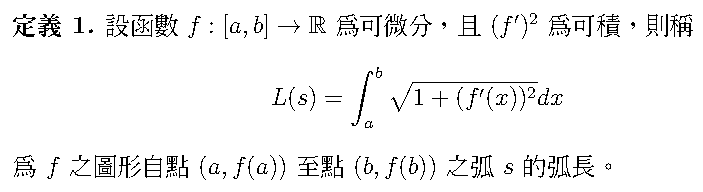
\includegraphics{cmath01}
\end{quote}

其中 {\ttfamily theoremstyle} 有三種 style,{\ttfamily plain, difinition, remark},預設使用的是 {\ttfamily plain},即定理名稱會用粗體字,內文則是 italic 斜體字,但這在中文並不適當,所以改由 {\ttfamily remark} style 來排版。要注意的是定理環境內的 {\ttfamily plain} style 雖然使用 italic 字型,但他並沒有進入數學模式,因此裡頭的數學式子仍然要進入數學模式來排版。另外,實數的那個特殊符號 $\mathbb{R}$ 要引用 {\sffamily amssymb} package 才會有,這也是美國數學協會\index{美國數學協會}發展的。


{\sffamily amsthm} 另提供了 \verb|\theoremstyle|\index{theoremstyle@\verb=\theoremstyle=} 給使用自行定義除了 {\ttfamily plain}、{\ttfamily definition} 及 {\ttfamily remark} 三種形式外的 style。另外,\LaTeX{} 本身的工具組也提供了一個 {\sffamily theorem} 巨集套件,能更有彈性的來細部微調,也有現成的指令,可以去改變所要使用的字體,可以參考系統上就有的 {\ttfamily theorem.dvi} 這個說明檔。

\section{數學模式中的字型及空間調整}

我們前面已有談到調整數學模式字體大小的四個指令。這裡我們再來看看其他的調整指令。

\subsection{數學字體的改變}

以下的指令,相信大家從他的簡寫就可以知道意思:

\begin{quote}
  \begin{tabular}{lll}
    指令                    & 作用        & 實例              \\
    \hline
    \verb|\mathrm| & 正常字體    & $\mathrm{ABCabc}$ \\
    \verb|\mathtt| & 打字機字族  & $\mathtt{ABCabc}$ \\
    \verb|\mathbf| & 粗體字      & $\mathbf{ABCabc}$ \\
    \verb|\mathsf| & sans serif  & $\mathsf{ABCabc}$ \\
    \verb|\mathit| & italic 斜體 & $\mathit{ABCabc}$ \\
    \verb|\mathcal| & 數學花體字  & $\mathcal{ABC}$
  \end{tabular}
\end{quote}

其他的套件會有更多的不同字體,請參考系統裡頭的 {\ttfamily symbols-a4.pdf}。要注意的是,有些字型並不是都完全有各種字體組合,像花體字並沒有小寫字母。

\subsection{數學模式中調整間距}

正常情況下,數學模式中的空間調整應不必使用者去操心,但程式畢竟不會思考,有些特殊場合仍然需要人為的調整。

\begin{quote}
  \begin{tabular}{llll}
    指令                    & 作用                   & 指令                    & 作用                 \\
    \hline
    \verb|\quad| & 空出一個 em 單位的空白 & \verb|\qquad| & 空出兩個 em 的空白   \\
    \verb|\,| & 加入 1/6 quad 的空白   & \verb|\!| & 減去 1/6 quad 的空白 \\
    \verb|\;| & 加入 5/18 quad 的空白  & \verb|\:| & 加入 2/9 quad 的空白
  \end{tabular}
\end{quote}

其中 \verb|\,|、\verb|\quad| 及 \verb|\qquad| 可以用在一般的文字模式及數學模式,其他的只能使用在數學模式中。我們把上一個弧長定義的例子來試著調整一下:

\begin{quote}
  \begin{verbatim}
 ...
\begin{cdefi}
設函數 $f:[a,b]\rightarrow{\mathbb R}$ 為可微分,且 $(f')^2$ 為可積,則稱
\[
L(s)=\int^b_a\!\sqrt{1+(f'(x))^2}\,dx
\]
為 $f$ 之圖形自點 $(a,f(a))$ 至點 $(b,f(b))$ 之弧 $s$ 的弧長。
\end{cdefi}
 ...
\end{verbatim}
\end{quote}

排版出來的結果是:

\begin{quote}
  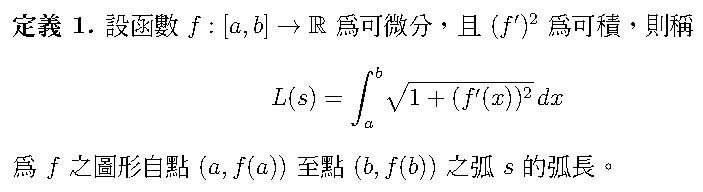
\includegraphics{cmath02}
\end{quote}

但是,要注意的是,如果文章有點長,數學式子也不少,那一定要注意整體的一致性,要調整的話就全文相同的地方都要去調整,否則就使用預設值就可以了,至少他不會太離譜。  % math.tex
% !TeX root = ../main.tex

\chapter{一篇文章、一本書的完整結構}
\label{ch:abook}

好了,寫文章最後也要整理成冊,這也是排版系統要負責的部份。如果只是簡單幾百、幾千字的小文章,那很容易,只要個文章題目,章節標題,那也就夠了。但如果是較正式的論文,那可能還有目錄、參考文獻、索引 \chdots{}等等,甚至一本書籍的話,也要有個封面,及送印刷廠時要用到的裁切記號(crop marks)\index{裁切記號(crop marks)}。如果要置放在網頁上的,那還得注意網路超連結互動的問題,所以,這些細節算是滿瑣碎的,但卻是必要的。

當然,個人也並不是什麼排版、印刷的專家,只能談談我所知道的事項,如果需要補充或修正,請有這方面經驗的朋友,不吝提供心得及指正。個人出版,這實際上不是夢,尤其網路發達的今日。

\section{目錄(Contents)\index{目錄}\index{Contents}}

目錄的問題,如果不講究的話,使用 \LaTeX\ 預設的就行了。就像第 \ref{sec;toc} 節所舉的例子一樣。但如果要做調整的話,除非熟悉 \LaTeX\ 巨集的寫法、定義,否則就得使用現成的巨集套件,例如 {\sffamily minitoc}\index{minitoc@\textsf{minitoc}} 可讓目錄更緊湊,{\sffamily titletoc}\index{titletoc@\textsf{titletoc}} 更可做相當幅度的調整及美化。

在 \LaTeX\ 文稿內,\verb|\tablofcontents| 可以排版一般的章節目錄。\verb|\listoffigures| 指令可以排版圖目錄,\verb|\listoftables| 指令則可排版表目錄。但圖表的話是指有進入浮動環境,使用 \verb|\caption| 指令,有編號的圖表而言。請注意,這些目錄指令的置放位置會影響實際目錄出現的順序,沒有特殊需求的話,一般的順序是文、圖、表。

\subsection{更改目錄標題名稱}

預設的情形下,在目錄開頭都會有個標題來引導,例如:\textbf{Contents}、\textbf{List of Figueres} 及 \textbf{List of Tables} 等,但是這在中文的情形看起來會不相稱,我們可以去更改預設值。更改 \LaTeX\ 預設值得視原來這個值是以什麼形式出現,在目錄是以指令定義的形式出現,所以我們要使用 \verb|\renewcommand| 這個指令去重定義他。

原來的這些 \textbf{Contents} 標題是怎麼「弄」出來的呢?如果手頭上沒有相當的參考書籍,可以參考他的原始定義,例如這篇文章是使用 {\ttfamily report} class,那麼找一下:

\begin{quote}
  \begin{verbatim}
/usr/share/texmf/tex/latex/base/report.cls  % Unix-like 系統
C:\texmf\tex\latex\base\report.cls          % DOS/Windows 系統
\end{verbatim}
\end{quote}

這個檔(依安裝的地方不同,可能會有不同的路徑),搜尋 Contents 這個關鍵字,就可以發現,他們原來的定義是:

\begin{quote}
  \begin{verbatim}
\newcommand\contentsname{Contents}
\newcommand\listfigurename{List of Figures}
\newcommand\listtablename{List of Tables}
\end{verbatim}
\end{quote}

這樣就清楚了,我們要重指定的是 \texttt{contentsname}、\texttt{listfigurename} 及 \texttt{listtablename}。其他的情形請依此類推。現在我們來把他改成中文:

\begin{quote}
  \begin{verbatim}
\renewcommand\contentsname{目~錄~}
\renewcommand\listfigurename{圖~目~錄}
\renewcommand\listtablename{表~目~錄}
\end{verbatim}
\end{quote}

這裡以 {\sffamily CJK}\index{CJK@\textsf{CJK}} 巨集為例,由於我們需要中文環境,所以這些更改要放在 \texttt{CJK} 環境中,如果只是更改成其他英文字樣,那我們置於 preamble 區就可以了。

\subsection{目錄的深度}

通常,有編號的章節或有 caption\index{caption} 的圖表才會編入目錄中,但如果想讓目錄的結構更細,那麼我們就得更改列入目錄的深度。目錄深度的表現形式是一種計數器(counter),他的名稱是 \texttt{tocdepth}。以這篇文章的 \texttt{report} class 為例,他的預設值是(請自行查一下 \texttt{report.cls}):

\begin{quote}
  \begin{verbatim}
\setcounter{tocdepth}{2}
\end{verbatim}
\end{quote}

所以會計算到 \texttt{subsection},以下的就不列入了(請參考第 \ref{subsec:chapstruc} 小節的章節深度標號)。我們只要在 preamble 區,使用 \verb|\setcounter| 指令去重新指定,就會改變他的目錄深度。

\subsection{額外的目錄}

這是指沒有編入目錄,但想自行加進去的情形,例如:章節指令使用了星號就不會編號,圖表目錄沒有使用 \verb|\caption| 指令,也不編入目錄了,這時我們可以使用 \verb|\addcontentsline| 指令來把他們手動加進去。我們來看看文圖表的三種不同情況:

\begin{quote}
  \begin{verbatim}
\addcontentsline{toc}{章節名}{標題}
\addcontentsline{lof}{figure}{標題}
\addcontentsline{lot}{table}{標題}
\end{verbatim}
\end{quote}

這樣就會把這些納入目錄,但是,這還是沒有編號的。目錄中所顯示的頁數,就是這些指令(圖表)所在的頁數。

\section{交互參照(Cross References)}
\label{sec:ref}\index{交互參照}\index{Cross References}

所謂的參照,指的是在文章某處提及某個其他的章節,或某個頁數,甚至是某個圖表,某個數學式子及某個列舉項目,排版系統必需要有這樣的功能來自動達成這種效果,而 \LaTeX\ 本身提供了三個簡單易用的指令來自動處理,他會自動計算相對的章節、頁數。

當然,由於網路的發達,超連結上的交互參照也變得是不可或缺,但 \TeX/\LaTeX\ 畢竟是平面排版系統,並沒有這樣的原始功能,但我們可以經由巨集套件來達成這樣的目的,{\sffamily hyperef} 巨集套件就是為此而寫的,這樣就可以讓 \LaTeX\ 排版的結果去轉換成 PDF/HTML 格式的時候,也有超連結的功能。

廣義的來說,包括目錄的參照、文獻參照、註解的參照及外部檔案的參照(例如,參照某個外部檔案的某個章節)都是屬於交互參照的一部份,但這些議題我們另外單獨討論,因為他不在 \LaTeX\ 所提供的三個基本參照的指令範圍內。

\subsection{一般的交互參照}

\LaTeX\ 提供了三組基本參照的指令:

\begin{quote}
  \begin{verbatim}
\label{名稱}    % 置放於要被引用之處,以一個名稱來標記他
\ref{名稱}      % 引用 \label 所標記處的章節
\pageref{名稱}  % 引用 \label 所標記處的頁數
\end{verbatim}
\end{quote}

這裡頭的名稱都是自行取名的,但為了避免重複,個人使用上一般使用上會加入章節或圖表的代號,例如:

\begin{quote}
  \begin{verbatim}
 ...
\section{\LaTeX\ 的文稿結構}
\label{sec:struct}
 ...
\begin{figure}
\includesgrapics{fontstruct}
\caption{字型的結構}
\label{fig:struct}
\end{figure}
 ...
請參考第 \ref{sec:struct} 節,頁 \pageref{sec:struct}。
請參考圖 \ref{fig:struct},頁 \pageref{fig:struct}。
 ...
\end{verbatim}
\end{quote}

這兩個 {\ttfamily struct} 代表不同的參照處,當然,盡量避免這種情形發生,可加入 {\ttfamily fontstruct} 之類的來區別,但前面冠上章節、圖表的簡名,有助於看文稿時清楚區別。請注意,其中 {\ttfamily sec:}、{\ttfamily fig:} 都不是必要的,只是這樣比較容易辨識,而且不容易名稱重複。

要非常注意的的幾個重點是:
\begin{quote}
  \begin{enumerate}
    \item 有參照的文稿一定要編譯兩次才能正常顯示。
    \item 能編號的章節、圖表、列舉項目、數學式、定理才能參照,雖然他們不一定要編號。
    \item 圖表的參照 \verb|\label| 一定要在 \verb|\caption| 之後,不能在前。
  \end{enumerate}
\end{quote}

\subsection{超連結交互參照(hyperlink)}

這當然是要像 PDF/HTML 格式的檔案才有超連結交互參照的可能,像 {\ttfamily *.dvi}、{\ttfamily *.ps} 這類格式的檔案,先天上並沒有這種設計。而 \LaTeX\ 本身並沒有內建這種功能,我們可以使用 {\sffamily hyperref}\index{hyperref@\textsf{hyperref}} 巨集套件來達成這個目的。現在一般的 \TeX\ 發行版本應該都會附上這個巨集,如果沒有話,可以在以下網站下載、安裝:

\begin{quote}
  \url{ftp://ftp.tug.org/pub/tex/hyperref/}
\end{quote}

這個套件會讓原本 \LaTeX\ 有交互參照的地方,在製作成 PDF 格式時也會有超連結的功能。他的設定檔是 {\ttfamily hyperref.cfg},為了各種文稿使用上的彈性,可以把這個檔在工作目錄上建立一個,這樣會依這個設定檔來執行,可參考本文文稿的原始碼,裡頭會有一個設定檔供參考。當然也是可以在 preamble\index{preamble} 區來設定,但這就只能使用在特殊的文稿上了。

他的使用方法,這裡不多做說明,可以參考本文的原始碼裡頭的使用方法,或參考〈由 \TeX/\LaTeX 製作中文 PDF 檔〉一文:

\begin{quote}
  \url{http://www.study-area.org/tips/latex/chpdf.html}\\
  \url{http://www.study-area.org/tips/latex/chpdf.pdf}
\end{quote}

及 {\sffamily hyperref} 所附的使用手冊。

\section{索引(index)}
\label{sec:index}\index{索引}\index{index}

索引的排版方法上並不算困難,困難的是要選出哪個字詞需要索引,及把各個字詞加入索引指令。我們引用 \LaTeX\ 的標準巨集 \textsf{makeidx}\index{makeidx@\textsf{makeidx}},並在其他加上一個 \texttt{makeindex}\index{makeindex@\texttt{makeindex}} 指令,然後在文稿結束前印出索引,下 {\ttfamily printindex}\index{printindex@\texttt{printindex}} 就可以了。我們在需要編入索引的名詞後加上 \verb|\index{名詞}|\index{index@\verb+\index+} 經過編譯後就會自動把索引及其相對的頁數計算出來。

\subsection{索引的結構及編譯}

我們來看看文稿裡頭要加入什麼要件:

\begin{quote}
  \begin{verbatim}
 ...
\usepackage{makeidx}
\makeindex
 ...
要索引的名詞\index{要索引的名詞}
 ...
\printindex        % 一定要有這個指令才會印出索引
\addcontentsline{toc}{chapter}{索引}  % 把他加入目錄
 ...
\end{verbatim}
\end{quote}

編譯的的程序如下:

\begin{quote}
  \begin{verbatim}
latex your.tex
makeindex your.idx
latex your.tex
\end{verbatim}
\end{quote}

\subsection{索引值的製作}

索引值(key)\index{索引!索引值}裡頭 \verb+|+、\verb|@| 及 \verb|!| 有特殊的意義,要索引他們時前面要加 {\ttfamily "} 來 escape 他。我們來看這些符號實際上有什麼作用:

\begin{quote}
  \begin{tabular}{ll}
    \verb|abc\index{abc}| & 這是一般正常的索引                        \\
    \verb|xyz\index{abc!xyz}| & 表示 xyz 是 abc 下的一個子索引            \\
    \verb+abc\index{abc|textit}+ & 表示這個索引值的頁數使用 italic 斜體排版  \\
    \verb|abc\index{abc@\textbf{abc}| & 表示索引值是 abc,但使用粗體排版          \\
    \verb|\'abc\index{abc@\'abc}| & 表示依 abc 來排序索引,而不是後面的 \'abc
  \end{tabular}
\end{quote}

製作索引是需要細心與耐心的,這方面更詳細的資料可以參考系統上的 {\ttfamily makeindex.dvi} 及 {\ttfamily manpages.dvi}。要注意的是 \verb|\index{}| 最理想是緊接在要索引的名詞後,前後都不留空白,有多個 \verb|\index{}| 相連時亦同,這會讓文件維護增加困難,因此,視每個人的習慣,可以考慮索引在整篇文稿最後才加進去。這份文件也製作了簡單的索引,但這只是當個例子供參考,在製作上有點粗糙,因此,實際上可能會漏掉很多,而且,中文的處理仍有待加強。

製作索引的時候,他的表示法要細心的注意一下,前後相同索引值的表示法要一樣,例如 \verb|\index{abc@\textbf{abc}| 和 \verb|\index{abc@{\bf abc}| 這會造成兩個不同的索引,雖然印出來的是一樣。而且,\verb=\verb|abc|= 這種方式就行不通,因為 \verb=|= 這個符號在索引指令內有他的特殊作用,要改用其他的符號代替。如果是和 {\sffamily hyperref} 配合的話,\verb+abc\index{abc|textit}+ 也會行不通,因為 {\sffamily hyperref}\index{hyperref@\textsf{hyperref}} 對超連結的索引是自動加上 \verb=|hyperpage=,如果已經有 \verb=|textit= 了的話,就不會加上去了,這樣一來超連結的部份會被忽略,解決的方法只能去重定義索引方法,或在編譯出來的 {\ttfamily *.idx} 或 {\ttfamily *.ind} 上做另外處理。例如:

\begin{quote}
  \begin{verbatim}
abc\index{abc|textit}
latex 編譯後的情形是:
\indexentry{abc|textit}{143}          % *.idx 檔
經 makeindex 編譯後的情形是:
\item abc, \textit{143}               % *.ind 檔
這樣只編號改變字體,並沒有超連結。而我們要的是:
\item abc, \textit{\hyperpage{143}}   % 這樣才能又變更編號字體又能超連結
\end{verbatim}
\end{quote}

這個議題比較深入一點,解決的方式可能需要大家一同來研究、研究,不是不能解決,而是方式在使用上是否方便的問題。

索引的處理,他的資訊實際上是產生在編譯後的 \texttt{*.idx} 檔裡頭,然後經由 \texttt{makeindex} 外部程式編譯後,轉換成 \texttt{*.ind},然後 {\ttfamily latex} 再次編譯的時候,才把這個 \texttt{*.ind} 引進來,這個 \texttt{*.ind} 其實就是一個 \LaTeX\ 的文稿,他把所有的索引值及頁數,包在一個 {\ttfamily theindex}\index{theindex@{\ttfamily theindex}} 環境中來引入排版的。

說明這些的用意就是暗示,我們可以由外部處理程式去動手腳,把索引的部份再「加工」,包括中文資料的處理也是一樣,下一節要談到的參考文獻的處理機制也是類似的情形,而這也就是為什麼 {\ttfamily latex} 要執行好幾次的原因,也正因為這樣,我們才有動手腳的機會,例如 {\ttfamily makeindex} 就有 {\ttfamily -s} 參數,可以接受外部的 style 檔,或者,如果工作目錄上有 {\ttfamily *.mst}(makeindex style)這個檔,也會優先去參考錈,這樣就可以產生不同形式的索引結果。當然,參考文獻可以另單獨的一個文獻外部檔,索引的話,目前則沒有辦法這樣做,是否可以比照參考文獻的做法,由外部檔案來處理呢?就請大家腦筋急轉彎一下了,這樣也可以讓文稿更容易維護。

\subsection{更改索引標題}

預設的索引標題\index{索引!標題}是 \textbf{Index}\index{Index@\textbf{Index}},我們可以在 preamble\index{preamble} 區來更改他(中文的話,請放在本文區 \texttt{CJK} 環境內),例如,設要中文名稱的話,可更改為中文:

\begin{quote}
  \begin{verbatim}
\renewcommand\indexname{索~引}
\end{verbatim}
\end{quote}


\section{參考文獻(Bibliography)}
\label{sec:biob}\index{Bibliography}\index{參考文獻}

參考文獻可以經由 \LaTeX\ 內建的 \texttt{thebibliography}\index{thebibliography@\texttt{thebibliography}} 環境來製作。長篇文稿,也可以使用 Bib\TeX\index{BibTeX@Bib\TeX} 由外部檔案來製作。至於參考文獻的格式,就要符合邀稿單位的規格了,這裡不多做說明。

\subsection{\texttt{thebibliography} 環境}
\label{subsec:thebibliography}\index{thebibliography@\texttt{thebibliography}}

在進入 \texttt{thebibliography},編譯後他會自成一個獨立的章節,如果是 \texttt{article} 類別的文稿,他會自動印出 \textbf{Referrences}\index{Referrences@\textbf{Referrences}} 的字樣為標題,如果是 \texttt{report} 或 \texttt{book} 類別的文稿,他會印出 \textbf{Bibliography}\index{Bibliography@\textbf{Bibliography}} 的字樣為標題。

在 \texttt{thebibliography} 環境裡頭,他是由 \verb+\bibitem+\index{bibitem@\verb+\bibitem+} 指令來列出資料的,我們來看一下他的語法:

\begin{quote}
  \begin{verbatim}
\begin{thebibliography}{99}  % 參考文獻印出之編號最寬為兩個字母寬
\bibitem[標記一]{鍵值一} 參考資料一
\bibitem[標記二]{鍵值二} 參考資料二
 ...
\edn{thebibliography}
\end{verbatim}
\end{quote}

所謂的「標記」這是選項參數,如果沒有的話,則正常引用後會在甲用處使用阿拉伯數字外加方括號來顯示;如果有加入的話,引用後會使用所加入的標記來顯示。那個「鍵值」指的就是引用時的關鍵字,後面所接的「參考資料」就是書籍、論文等資訊。其中的 \verb+{99}+ 只表示在最後的參考文獻印出來的時候,最開始的編號統一在兩個字母寬,如果都沒有使用「標記」,那麼就是兩個數目字寬,如果有使用「標記」,那麼要設在最長標記的字母寬,否則印出時會無法對齊。

我們引用的時候是使用 \verb+\cite{鍵值}+\index{cite@\verb+\cite+} 這個指令,他會顯示參考資料中的編號值,且以方括號括起來。我們來看看一些設定及引用的例子,:

\begin{quote}
  \begin{verbatim}
\begin{thebibliography}{KDE}  % 參考文獻中印出的編號最寬為三個字母寬
\bibitem{KDEt} Knuth, D.E., \textit{The \TeX{}book},
Reading, Massachusetts: Addison-Wesley, 1989.
\bibitem[KDE]{KDEm} Knuth, D.E., \textit{The \MF{}book},
Reading, Massachusetts: Addison-Wesley, 1986.
 ...
\end{thebibliography}
\end{verbatim}
\end{quote}

參考文獻印出的結果請參考本文件後面關於參考資料的部份。至於引用方式及其引用情形如下(顏色的部份是因為使用 {\sffamily hyperref} 套件的超連結):

\begin{quote}
  \begin{tabular}{ll}
    引用方式                       & 引用結果                 \\
    \hline
    請參考 \verb+\cite{KDEt}+ & 請參考 \cite{KDEt}       \\
    請參考 \verb+\cite[1989]{KDEt}+ & 請參考 \cite[1989]{KDEt} \\
    請參考 \verb+\cite{KDEm}+ & 請參考 \cite{KDEm}       \\
    請參考 \verb+\cite[1986]{KDEm}+ & 請參考 \cite[1986]{KDEm} \\
    請參考 \verb+\cite{KDEt,KDEm}+ & 請參考 \cite{KDEt,KDEm}
  \end{tabular}
\end{quote}

如果你現在是在觀看 PDF 格式的檔案,那在 {\sffamily Xpdf}\index{Xpdf@\textsf{Xpdf}} 或 \textsf{Adobe Acrobat Reader}\index{Adobe Acrobat Reader@\textsf{Adobe Acrobat Reader}} 都可以使用滑鼠來點一下,看看真正在後面印出時是什麼樣子。再次強調,參考文獻的規格請依邀稿單位的要求,這裡所列出來的不是「標準」。

\subsection{更改標題名稱}

前面已提到過更改目錄及索引的標題,同樣的方法,我們也可以更改參考資料的標題,只是要注意引用的文稿類別是什麼。

\begin{quote}
  \begin{verbatim}
\renewcommand\refname{參~考~資~料}  % article 類別文稿
\renewcommand\bibname{參~考~文~獻}  % report/book 類別文稿
\end{verbatim}
\end{quote}

\subsection{Bib\TeX\ 簡介}
\label{subsec:bibtex}\index{BibTeX@Bib\TeX}

如果常常有寫論文的機會,整理出自己的一份參考文獻資料庫可以節省許多時間,正常情況下,使用 \texttt{bibtex} 來處理外部文獻檔案的情形,只有引用到的文獻才會印出來,這樣也就不必擔心印出一堆不相關的文獻了。另外一個好處是,這個參考文獻資料庫可以另外獨立維護,所有的文章都用這一份資料庫,這在維護上會很方便,也減少錯誤的機會。

Bib\TeX\ 本身提供一個外部的 \texttt{bibtex}\index{bibtex@\texttt{bibtex}} 工具程式,在 \texttt{latex} 編譯過文稿後,再利用 \texttt{bibtex} 編譯一次文稿,最後再使用 \texttt{latex} 重編譯過。而參考文獻資料庫是按一定的格式寫於 \texttt{*.bib} 檔案裡頭,在文稿中則以 \verb+\bibliogrphy+ 指令來引入,編譯過程中自然會去參考這個外部考文獻資料庫。他的使用情形如下(以 \texttt{your.bib} 為例):

\begin{quote}
  \begin{verbatim}
 ...
\begin{document}
\bibliogrphiystyle{plain}  % 指定 style 檔
 ...
\bibliography{your.bib}    % *.bib 延伸檔名可以省略
 ...
\end{document}
編譯過程:
latex example
bibtex example
latex example
\end{verbatim}
\end{quote}

\subsubsection{\texttt{*.bib} 檔的格式}

\texttt{*.bib} 檔的格式自成一格,和寫在原來文稿裡頭的不同,視資料的性質,要把他標明出來,例如書籍類是 \verb|@book| 來開頭,期刊文章使用 \verb|@article| 來起頭,我們來看一個例子:

\begin{quote}
  \begin{alltt}
    @book\{ KDEt,
    \textcolor{red}{author}      = "Knuth, Donald E.",
    \textcolor{red}{year}        = "1989",
    \textcolor{red}{title}       = "The \verb|{\TeX}|book",
    \textcolor{red}{publisher}   = "Addison-Wesley",
    address     = "Reading, Massachusetts",
    volumn      = " ",
    edition     = " ",
    month       = " ",
    series      = " ",
    note        = " ",
    \}
    @article\{ somekey,
    \textcolor{red}{author}      = "Someone",
    \textcolor{red}{year}        = "2004",
    \textcolor{red}{title}       = "The \verb|{\TeX}| Journal",
    \textcolor{red}{journal}     = "SayYa-Publisher",
    volumn      = " ",
    number      = " ",
    pages       = " ",
    month       = " ",
    note        = " ",
    \}
  \end{alltt}
\end{quote}

每行後的逗點是必要的,名字的話 \texttt{Knuth, Donald E.} 或 \texttt{Donald E. Knuth} 這兩種方式,\texttt{bibtex} 都能認得,但姓擺在前面的時候其後要加個逗點,如果是兩位以上的作者時要以 \texttt{and} 來連接。雖然可以使用 \LaTeX\ 的語法,這時他整個要由大括號括起來,而且,註解符號 \texttt{\%} 不被接受。紅色的項目是必要的項目,其他項目可以列進去,也可以省略,要加進去的話,則以 \texttt{" "} 空出來,這樣以後有這方面的資料時再填進去。

顯現的形式是受 \text{*.bst} 格式檔在控制的,所以,不必要的標點符號不要自行加進去,書名的字體顯示也無需加進去。

引用的方式同樣是使用 \verb|\cite| 指令,一般只要要引用到的資料才會印出來,如果要全部 \texttt{*.bib} 裡頭的資料都印出來的話,可以加個 \verb|\nocite{*}| 指令。

在使用中文的情形下,\texttt{bibtex} 程式認不得中文,在 \texttt{CJK}\index{CJK@\texttt{CJK}} 環境下編譯會出問題,我們可以先編輯一個 \texttt{*.cbib} 檔,然後再使用 \texttt{bg5conv} 來把他轉成 \texttt{*.bib} 檔:

\begin{quote}
  \begin{verbatim}
bg5conv < some.cbib > some.bib
\end{verbatim}
\end{quote}

這樣,在文稿裡頭引入 \texttt{some.bib} 就可以了。

\subsubsection{格式檔}

Bib\TeX\ 的格式檔是 \texttt{*.bst}(bibliography style),我們上面所引用的是 \texttt{plain} 其實就是引用 \texttt{plain.bst} 這個格式檔,這是最基本的格式,在編譯時期會依這個格式檔來印出參考文獻的顯現形式。其他尚有:

\begin{quote}
  \begin{tabular}{>{\ttfamily }ll}
    plain & 依字母的順序印出,比較順序為 author, year, title                        \\
    unsrt & 依引用的先後次序印出                                                    \\
    abbrv & 與 \texttt{plain} 相同,但 first name, month, title, journal 以縮寫印出 \\
    alpha & 引用處顯示 [作者年份] 來取代數目字。
  \end{tabular}
\end{quote}

已經有許多人發表過特定的格式檔,但這些對於中文則無法完全合乎我們的使用習慣,例如標點符號及書名號,但我們可以去更改他們的格式,這方面的資料請參考系統上的 \texttt{btxdoc.dvi} 及 \texttt{btxhak.dvi} 這兩個說明檔。

這也算是目前的一個值得去研究的空間,尤其是中文及 Unciode 編碼文件索引、排序及排版的問題,這在英文語系算是比較容易解決,都有現成的格式範例可以運用,但中文就比較缺乏這方面的範例。在吳聰敏教授的《\texttt{cw}\TeX\ 排版系統》\cite{cwtex} 一書裡頭,有對這方面做過努力,使用的是外部程式工具 \texttt{cwbibtex},再和 \texttt{cw.bst} 格式檔配合的話,有不錯的結果。

\section{附錄(Appendix)}

排版附錄使用的是 \verb|\appendix| 指令,這個指令以後和正常一般編輯即可,不同的附錄以 \verb|\chapter| 來區隔,但印出來的時候會標上大寫字母,而不是原來的 \textbf{Chapter} 字樣。也是可以有 \verb|\section| 指令,這資了大寫英文字母外,會緊接著附上阿拉伯數字,例如 \textbf{A.1}、\textbf{B.2} 等等。

\subsection{改變附錄的標題}

在英文環境,附錄是以 \textbf{Appendix} 為標題來開始的,在中文環境下我們要把他改成中文:

\begin{quote}
  \begin{verbatim}
\renewcommand\appendixname{附~錄}
\end{verbatim}
\end{quote}

\texttt{article} 類別的文稿並不印出 \textbf{Appendix} 字樣,因此也就沒有 \texttt{appendixname} 來更改。

\section{大型文稿的維護}
\label{sec:largefile}

通常我們寫一篇文章,大概都是一個文稿寫到底,但如果超過一百頁的文稿的時候,維護起來會比較困難,所以 \LaTeX\ 提供了 \verb|\input| 及 \verb|\include| 指令來將外部檔案引進來,當做是文稿的一部份來編譯,這樣就可以按章節來把文稿分開處理、維護。

他們的使用方法很簡單,一個是含主要正常結構的主檔,其他的則沒有 preamble 區,只有本文區,就是按照一般文稿中的章節的部份來書寫就可以了。以這一篇文件的例子來說,他的主檔是 \texttt{latex123.tex},主要的內容如下:

\begin{quote}
  \begin{verbatim}
\documentclass[12pt,a4paper]{report}
 ...
 這裡是 preamble 區的內容
 ...
\begin{document}
\begin{CJK}{Bg5}{hwmm}
 ...
%begin{latexonly} 
% ``�j�a�Ӿ� LaTeX'' LaTeX ��Z story.tex
% Copyright (c) 2004  Edward G.J. Lee <edt1023@info.sayya.org>
%
% �b���H�� GNU Free Documentation License 1.2 �ΥH�᪺�����W�d���U�A
% ���\�����B���G�έק�C�����v�B���v�n�����o���B�����C
%
% �����G�����A�t�� fdl.tex�A���e�� GNU FDL ���W�d���C�p�G�򥢡A�i��
% http://www.gnu.org ���o�A�μg�H�ܦۥѳn�����|(Free Software Fundation)
% �����C
% 9 Temple Place - Suite 330, Boston, MA 02111-1307, USA.
%
% $Id: story.tex,v 1.26 2004/03/07 12:30:58 edt1023 Exp $
%
\chapter{���ӻ��@�ǬG��}

\TeX\ �O
Donald~E.~Knuth\footnote{\url{http://www-cs-faculty.stanford.edu/~knuth/}}\index{Donald~E.~Knuth}
�бª���߳ǧ@�A���O�ӥ\��D�`�j�j������ƪ��t�ΡA�t���u�ʫܤj�A�ӥB�ܧC�����ƪ��y���C����A�O�]�� Knuth �б¦b�g�L���j�� TAOCP(\textit{The Art of Computer Programming})\index{TAOCP}
�ɡA�oı�Ѱӧ�L�Ѥ����ƾǦ��l�Ʊo�����ݤF�A��O�M�w�ۦ�}�o�@�ӫD�`�A�X�ƼƾǦ��l���ƪ��y���A�o�N�O \TeX\ �t�Ϊ��ӥѡC

���ȶȬO�ͨ� \TeX\ �@�w�|���� Knuth �б¡A�u�n����ƪ��A�S���H�i�H�����L�� \TeX\ �ұa�Ӫ��ܭ��B�v�T�A�Ʀ� \TeX\ �w�g 20 �X���F�A���M�`�`�v�T�۱ƪ��ɤαƪ��n��A�i���o�ӱƪ��n��u���O�D�P�p�i�C

\section{Knuth �бª��ͥ�²��}

\begin{quote}
\begin{tabular}{lp{.78\textwidth}}
1938.01.10  & �ϥ͡CMilwaukee, Wisconsin; U.S. citizen�C\\
1956        & �i�J�ͫ�u�ǰ|�]Case Institute of Technology�^�Dzߪ��z�C\\
1960        & ���~��i�J�[�{�z�u�ǰ|�]California Institute of Technology�^��s�ҡA������V�ƾǻ�쪺��s��V�C\\
1961.06.24  & �M Nancy Jill Carter ���B�C�L������W�r�O���w��\index{���w��}�A�L�ѱC�W�s������\index{������}�A�ѱC�p�L�@���C��Ӥp�ġA�@�k�@�k�C����W�r�O 1977 �h����j���ɨ����C\\
1963        & ���� Ph.D.�A�ïd�ե��СC\\
1968        & �}�l���Щ� Stanford �j�ǡA��T��Ǩt(Computer Science)�C�P�~�}�l���g�W�D�I�⪺ TAOCP({\em The Art of Computer Programming})�C���H�����A�ݤF�o���ѡA�����g�{�������D���|�ܱo����C:)\\
1977        & �����N�ѰөҦL�X�� TAOCP�A�]���A�ۦ�}�o \TeX\ �ƪ��t�ΡA�o�i�N�v�T�F���᪺�ƪ��B�X���ɡA�ܤ����Y�C���]�]���쩵�F TAOCP �ĥ|�U�������ɶ��C\\
1986        & �a�� ACM �n��t��C
\end{tabular}
\end{quote}

�L�i���O�ۧ@�����A���y�B�פ峣���A�L������ۧ@���ө_�Ǫ��y�Ƨ@�Ρz�A���N�O����H�o�{�ѤW�����~�A���i�H�V�L�|�o�A�û�� \$2.56�]�����^�I�Q�ոլݡu���v�ܡH�x�W�N���H��L�C:-) ������O \$2.56�HKnuth �бª����׬O�G

\begin{quote}
\it
``256 pennies is one hexadecimal dollar.''
\end{quote}

�o�{ \TeX\ �t�Ϊ����Τ]�O�@�ˡA�o�Ӽ����C�~���ƼW�[�A���� \$655.36($2^{16}$ pennies) ����C

�L�]�ܱ��R�ۥѳn�����| (Free Software Foundation)%
\footnote{\url{http://www.fsf.org}}\index{�ۥѳn�����|}\index{Free Software Foundation}
�� GNU/Linux\index{GNU/Linux}�A��@�ǧƱ泣�H�U�� GNU/Linux�A�ר�O Unicode ���ҡA�L�Ʊ� GNU/Linux �ܧִN��b�����W��ܥL������W�r�A�Ӥ����ϥι��ɡC���O�i�H����F�A�u�O Unicode �����٤��ⴶ�ν}�F�C�L���b 1996 �~���� Dr.~Dobb's~Journal �X�ݮɭ^�����^�������}���ܡA�оɦۥѳn�� (Free Software)%
\footnote{\url{http://www.gnu.org/philosophy/free-sw.html}}\index{�ۥѳn��}\index{Free Software}
�� Richard~M.~Stallman\index{Richard~M.~Stallman} �O�L�ߥؤ����^�����@�A�L�{���ۥѳn�����|�o�ǤH�Ұ����^�m�ܤ����A���M�M�L���覡���@�w�@�ˡA���\�h�^�m�O�����{�P���C

�b�o�i \TeX{} �ɴN�P�ɫ�� WEB�]�o�ӵ���ثe�ϥΪ� WWW Web �٦��ϥΡ^\index{WEB}�A���O�@�� literate programming\index{literate programming} ���{����k�C�L�{���ثe�w�������i�H���X�t����󪺵{����k�A�ϼg�{���N���g��ǧ@�~�]�p���H�^�@�몺���N���{�C��Ӥ]��L�� C ��g�]�M Silvio~Levy\index{Silvio~Levy} �X�@�^�A�W�� CWEB\index{CWEB}\index{CWEB}%
\footnote{\url{http://www-cs-faculty.stanford.edu/~knuth/cweb.html}}�C\TeX\ �N�O�� WEB �g�����AWEB �i���� Pascal �y�����@�Ӥl���C

�@�� literate �{���v�i�Q������ǧ@�a�B���׼g�@�̡B�H���@��\chdots{}�A�{�������{���ȶȬO�h�˲Ÿ��A�ӬO�i�{�ۤv������A���M�]�O���F���ت�������B�Ʀܵ{�����ܼƹB�Ϊ�����C

�o�ˤ@�ӴN�i�H�i�{���H������z�Ѫ��{���X�C�ϥΧΦ��ΫD�Φ����ĦX�A�ӥB��̶��ۻ��ۦ��A�ت��F���F�A�]���\Ū���H�N�n��Ū��ǧ@�~�몺�h����@�̪��ߡA�ϵ{���Ч@���ɦܧ󰪪��]��ǡ^���N�ҬɡA�Ӥ��A�O���O�O�� code �F�C

Knuth �j�v�w�� 1992 �~�ۤj�ǰh��A�����b Stanford/Oxford ���j�Ǧ��½ҡC�ثe���B�����~���ͬ��A�L�o�򦭰h�𪺭�]�A�N�O�]�� TAOCP �o���ѡA�L���p�j���n�� 20 �~�ӧ����A�]���ثe�����I�u�@�O�����L�� TAOCP�]�����n�X�U�A�ثe�u���X�����u���T�j�U�^�C�L�{��
email\footnote{\url{http://www-cs-faculty.stanford.edu/~knuth/email.html}}
�|�v�T�L������A�]���A���@�d���}�A�n�M�L�p���N�u�n�g�H�A�ǯu�C���L�����Ѫ� email�A�O�̫ᦳ�ɶ��~�|�h�ݡA�L�����}�������A�o���ѬO�L�o�@�ͤ��̭��n���u�@�C

���M Knuth �б¼g�F�\�h�Y���}�`�����y�B�פ�A���O�L�]�O�����쪺�@���A�b 1996 �~�A\textit{Mathematisch Centrum }(MC, ���y�����Q�P�~�y��٬� \textit{Centrum voor Wiskunde en Informatica}, CWI) ���ܽХL�t���A�ê��|������ \TeX\ User Group(NTG)%
\footnote{\url{http://www.ntg.nl}�A������ \TeX\ User Group ��O�۷����D���C}�ANTG �����|���o�A�N�ܽ� Knuth �б¥t�}�� \TeX\ �� \MF\ �Q�׷|�A�ñ����j�a�����ݡA�L���G�y����A�ڤ]�O�i�H�ݧA�̰��D���I�z�C�ӥB�A�L�ٻ��G�y�o�ذݵ������e�A�ܥi��b���P���X���ƹL�A�ҥH�A�p�G�ڹ�P�@�Ӱ��D�A�����L��ص��ת��ܡA�A�̥��ݨ��䥭���ȡC�z�L�����y�p�]�A�b�\�h���������X�`�`�ް_����j���A����ڪ����e�o���D�x�x�����C:-)


\subsection{TAOCP(\textit{The Art of Computer Programming})\index{TAOCP}\index{The Art of Computer Programming@\textit{The Art of Computer Programming}}}

�o�i�O�t��k���j�ۡA�ЧO���˧ڡA�ڥu�O���Q�����A�o���ѧڨS���@���O�ݱo�����C:-)

\begin{quote}
\begin{enumerate}
\item �Ĥ@�U�A{\em Fundamental Algorithms}�A1968 �Ĥ@���AISBN 0-201-89683-4�C
\item �ĤG�U�A{\em Seminumerical Algorithms}�A1969 �Ĥ@���AISBN 0-201-89684-2�C
\item �ĤT�U�A{\em Sorting and Searching}�A1973 �Ĥ@���AISBN 0-201-89685-0�C
\item �ĥ|�U�A{\em Combinatorial Algorithms}�A�|�������A�i��|���X���U�C
  \begin{enumerate}
     \item ���U 4A, {\em Enumeration and Backtracking}
     \item ���U 4B, {\em Graph and Network Algorithms}
     \item ���U 4C, {\em Optimization and Recursion}
  \end{enumerate}
\item �Ĥ��U�A{\em Syntactic Algorithms}�A�p�� 2010 �~�����C
\item �Ĥ��U�Athe theory of context-free languages�A�ѦW�i��|�ܧ�A�|���}�l�C
\item �ĤC�U�ACompiler techniques�A�ѦW�i��|�ܧ�A�|���}�l�C
\end{enumerate}
\end{quote}

�ԲӪ��ؿ��j���έ׭q������T�A�аѦҺ����W����ơG

\begin{quote}
\url{http://www-cs-staff.stanford.edu/~knuth/taocp.html}
\end{quote}

\section{����A\LaTeX\ �S�O����O�H}

\TeX\ �O�ӫܧC�����ƪ��y���A�p�G�ƪ��ɳ��n�q�o�اC���y���ӱ�������ܡA���N�|�D�`���нơA�ҥH�A�@�Ǹg�`�n�Ψ쪺�\��A���|���h�w�q�n�]�٬������Amacro\index{macro}\index{����}�^�A�o�˱ƪ��ɤ~�|��K�B�ֳt�A�����ޥΤw�w�q�n���������Y�����O�N�i�H�F�C

��l�� \TeX\ �w�g���F�@�� macro�A�O Knuth �б©Ҽg���A���N�O�ۦW�� Plain \TeX\index{Plain \TeX}�A�����M������K�B���[�A��O
Leslie~Lamport\index{Leslie~Lamport}\footnote{Leslie~Lamport �� 1985 �b
\htmladdnormallink{CSL}{http://www.csl.sri.com/}
��¾�ɼg�F \LaTeX�C�ثe��¾��
\htmladdnormallink{DEC Systems Research Center}{http://www.research.digital.com/SRC/home.html}
���w�X�G�S���ѻP \LaTeX\ ������o�i�F�C}
�S�g�F�t�@�ժ� macro�A�٬� \LaTeX�A�D�n�O�⪩���t�m�M�峹���e�A�A�ת����}�B�z�A�u�n�ϥΪ̿�w�F�@�����O�A�㥻�ѩξ�g�峹�����c�N�O���ӳo�����O�Ӧw�ƪ����A�o�˼g��󪺤H�u�n�M�`��峹���e�N�i�H�F�A�����t�m�N�����浹 \TeX{}/\LaTeX\ �h�B�z�C

�J�M \LaTeX\ �u���L�O \TeX\ ���@�j�ե����A���A���M��Ӫ� \TeX\ �����O�A�j�����]�O�i�H�Φb \LaTeX\ ��Z�������C�ӥB�A\LaTeX\ �ä��O�ثe�ߤ@�� \TeX\ macro�A��L�p eplain \TeX{}, Con\TeX{}t, \TeX{}info �����O \TeX\ macro�A�]�����L�̦ۦ��@�M���y�k�C�ثe�� \LaTeX\ ��
\LaTeX\ 3 Project\footnote{\url{http://www.latex-project.org/latex3.html}}
�Һ��@�εo�i�C


�p�G�ͨ�o�̡A�A�٬O���ٷ٪��ܡA���� HTML markup �аO�y���N��j�����D�@�Ƿ����F�A���M�A�o�M HTML �аO�y���O�i�۴��ӵL�k�ýת��C�p�G�s HTML �]�����x�A���]�S���Y�աI�o�����ӴN�O�b���G�ƹ��I:-) �u�n�~��ݫ᭱�����e�N��F�C

\section{�@��H�� \LaTeX{} ���g��}

�o�̤ޥ� Peter Flynn\index{Peter Flynn} �b�L��
\textit{A beginner's introduction to typesetting with \LaTeX{}}\footnote{\url{ftp://ftp.dante.de/tex-archive/info/beginlatex/beginlatex.pdf}}
�@�夤�Ҵ��X�Ӫ����j�g��A�òK�[�ӤH���@�Ǭݪk�G

\begin{itemize}
\item \LaTeX{} �u��ϥΤ@�ئr���H\\
���M���O�A���M \TeX{} �t�ιw�]�O�ϥη��� Knuth �б©ҳ]�p�� \MF�A���ثe OpenType, TrueType, Adobe Type1 �r�����i�H�Φb \LaTeX{} �����A�u���L�A�w�˦r�����������O���򪺪��[�N�O�F�A����_��L���ƪ��t�ΡA\TeX/\LaTeX\ �ү�Q�Ϊ��r�������A�i�H���O�̦h���C

\item \LaTeX{} �u��Ω� Unix-like ���@�~�t�ΡH\\
Knuth �бºB�n���� \TeX{} ����l�{���X�}��X��\footnote{���M���@�Ǫ��v���W�w�A���O Knuth �бª����N�A�o�ǭ�l�X�O�ݩ� Public Domain�A�u�O�A�p�G�g�L�ק�A����A�H \TeX{} ���W�A�n�t�~��@�ӦW�١A�H�K�M��Ӫ� \TeX\ �d�V�C\TeX\ �o�ӰӼЪ��Ҧ��H�O����ƾǨ�|�]American Mathematical Society, AMS\index{AMS}\index{American Mathematical Society}�^�C}�A�ҥH�A�u�n�O���H�b�ϥΪ��@�~�t�γ��i�H���ӹL�h�A������ߪ��v�����D�C�� MS DOS, OS/2, MS Windows, Mac OS, Unix-like �t�γ��� \TeX{} �����Ӫ����A�ƦܬO PDA�]e.g.~the Sharp \textsl{Zaurus}�^���� \TeX/\LaTeX\ ���a��C�i�H���O�������A�N�i�H�Ψ����A�ӥB�A��Z���O���q���A�C�L���G�]�ۦP�C

\item \LaTeX{} �w�g�L�ɤF�H\\
��n�ۤϡA\LaTeX{} Project\footnote{\url{http://www.latex-project.org/}}
�Ψ�L���� packages ��í�w����o�����A�ר�M�ثe�s�@�N�� SGML/XML/HTML �θ�Ʈw�t�ΡA���n�����Q��k�α��_�ӡC���ƾǦ��l���ƪ��A�ܤ��L�H��X��k�C�����쪺�ܡA�i�H�Ѧ� \url{news://comp.text.tex} ���y�q�A�Ψ䤤
\textsc{CTAN}\footnote{\url{http://tug.ctan.org/}}\index{CTAN}
��󥨶���s�B�W�Ǫ������o���C

\item \LaTeX{} �S���Ҩ��Y�ұo�]WYSIWYG\index{WYSIWYG}�^�H\\
�Y�ؼh���W�Ө��A�O���C�]���L����W�O����ƪ��t��\index{����ƪ��t��}�C���O�A�Ҳ��ͪ� dvi/ps/pdf �ɡA�i�H�ܺ�Ǫ���ܧA�ҷQ�n���F�����e�A����o�o�⤣��O�u�Ҩ��Y�ұo�v�H�t�~�A�@�Ǭ��� GUI �t�X���n��A�]�|���}����ƪ����w�q�A�Ҧp
LyX\footnote{\url{http://www.lyx.org/}}\index{LyX},
\TeX{}macs\footnote{\url{http://www.texmacs.org/}}\index{TeXmacs@\TeX{}macs}
�����C

\item \LaTeX{} �����ǡH\\
�o�ӹ��I�ڥu�໡�A������F��O�ܦn�Ǫ��H�p�G�u�O�@��ϥΡA�Ӥ��O���ӱƪ��M�a�A�Ʀ� \TeX/\LaTeX\ programmer�A����A�X�Q�����������A�N�i�H�u�W�u�v�F�I�ѤU���u�O�@�Dzӳ��վ㪺���D�]���h�վ�A�]���藍�|���С^�C�۹��@��ϧΤ� Office ���n��A�n�u����L�����e���x�A���Ȥ]�O��²�檺�C�t�~�����D�A�j���O���e�B����t�ξާ@�ߺD�����D�A�ƦܬO�@�زĤ@�L�H�F�A�N�n������q���A�����֤H�����l�̴N�|�B�{ MS Windows ���϶H�@�ˡC:-)

\item \LaTeX{} �O�M����Ǯa�μƾǮa�Ӽg���H\\
���T�A���� Knuth �б¬O���F���F��T�B�~���u�����ƾǦ��l�Ӷ}�o \TeX{} ���A���ѩ� \TeX{} ���u�ʡA�ϱo�b��L����쪺�ϥΪ̤]���ۨϥΡA�w�g���O�����b�dzN�ɦb�ϥΤF�C�ר� XML\index{XML} �����_�A�ݭn�@�ӾA�X���榡�Ƥu��]formatter\index{formatter}�^���t�X�A\TeX/\LaTeX\ �N��n��¾�����L�ƪ��M�~���u�@�C

\end{itemize}

\section{���媺���I��V}

\TeX/\LaTeX\ ������ij�D�G�������t�m�B�ƪ��W�d�B�r���޳N�B\TeX\ the program ����i�Bø�ϧ޳N�B\TeX\ macro �����g�Bpre/post �B�z�{�������g�B�X���y�{\chdots{}�����A�E�v�L�P�A�i�H���a�@���l�]�i���s�����A�ҥH�A�U��b�u���J�v�o�ӻ�줧�e�A��ij�̦n���ӾA�����d��A�H�K�u�U���U�`�v�צܵL�k�۩ޡC

�ҥH�A���媺���I�O��b�u�зǡv\LaTeX\ �����A��L������ package/macro ���D���n�A�ɶq�����ΡC���O \LaTeX\ �����]���O�Q���Q�����A�ҥH�A���ݭn���a��]�ݭn�@�ô��Υ~�Ӫ� macro�A�L�צp��A���I�O��b�з� \LaTeX\ �����A�о\Ū���媺�B�ͪ`�N�@�U�o�Ӥ�V�C\LaTeX\ �����N��ѨM���A�N�����~�D�F�A���M�|���h�F�@�Ǽu�ʡA�����K�y�� package/macro ���ѭ��A���þDz߰}�}�A��}�l�]�u�n�p���F�I

�ӥB�A�i�઺���ΤU�A�|���@��γ~����V�h���СA�Ӥ��ȶȱM�`�b�Ʋz�ƪ��C�ƾǦ��l���O \TeX/\LaTeX\ ����������A�����N���@��γ~�N���A�X�A�ۤϪ��A�{�b���\�h�ӷ~���q���� \TeX/\LaTeX\ �Ω�@��ӷ~�X���W�C


% ``�j�a�Ӿ� LaTeX'' LaTeX ��Z preparation.tex
% Copyright (c) 2004  Edward G.J. Lee <edt1023@info.sayya.org>
%
% �b���H�� GNU Free Documentation License 1.2 �ΥH�᪺�����W�d���U�A
% ���\�����B���G�έק�C���쪩�v�B���v�n�����o�����C
%
% �����G�����A�t�� fdl.tex�A���e�� GNU FDL ���W�d���C�p�G�򥢡A�i��
% http://www.gnu.org ���o�A�μg�H�ܦۥѳn�����|(Free Software Fundation)
% �����C
% 9 Temple Place - Suite 330, Boston, MA 02111-1307, USA.
%
% $Id: preparation.tex,v 1.23 2004/03/07 12:19:47 edt1023 Exp $
%
\chapter{��e�dz�}

�ϥ� \TeX/\LaTeX\ �t�ΡA��}�l�A����·Ъ��O�w�˰��D�C���L�A�H�{�b���@�~�t�ΦӨ��A�X�G���y�檺�@�~�t�γ����{���]�n�� \TeX\ �t�ήM��i�H�w�ˡA�Ҧp Un*x �t�Ϊ� te\TeX\index{teTeX@te\TeX}�BWindows �t�Ϊ� MiK\TeX\index{MiKTeX@MiK\TeX} �� fp\TeX\index{fpTeX@fp\TeX}�C�t�~�A�]��
\TeX\ Live CD\footnote{\url{http://tug.org/texlive/}}\index{TeX Live CD@\TeX\ Live CD}
�i�H�ѤU���B�ʶR�A�o�O
TUG(\TeX\ User Group)\footnote{\url{http://www.tug.org/}�C�[�J�|�����ܡA�u�n�dz\�|�O�A�h�i�H��o \TeX\ Live CD �Φ~����T���H�o�C}
�s�@���U�ا@�~�t�Ϊ��i�����ɡA�ϥΤW�۷���K�C

�ثe�ҿת� \TeX\ �M��A�O���Ӫ� \TeX\ �ƪ����������A�[�W \LaTeX\ �Ψ�L�����������A�A�[�W�r���n��]\MF{}�^�Bø�ϵ{���]\MP{}�^�B�r����\chdots{}�����A�ҲզX�����@��ӥi��ڹB�@���ƪ��t�ΡC�]���A����O \TeX{}�H�|�]�ϥΪ����X���P�Ӧ����P���N�q�A�@��«����O�������ɭԡA�N��¼g���p�g�� {\tt tex}�A���ɩҥΪ������A�w�]�N�O Knuth �б©Ҽg�� plain \TeX�C�g�� \TeX\ �ɡA�@��O����Өt�ΦӨ��C�o�b \LaTeX\ ������P�A{\tt latex} �����O���O�A\LaTeX\ �����O��ӥ����t�ΡC


\section{Unix-like �t��}

�@�� Unix-like �t�γ��O�w�� te\TeX\ �M��A�Z�O�M {\tt tetex} �r�ˬ����� packages ���w�˰_�ӡA�ثe GNU/Linux\index{GNU/Linux} �U�� distribution �� FreeBSD\index{FreeBSD} �����{���� packages �Ѧw�˨ϥΡC�p�G�O�S�����ѳo�ӮM�󪺧@�~�t�ΡA�i��o�ۦ�sĶ�F�A��l�X�b�G

\begin{quote}
\url{http://www.tug.org/teTeX}\\
\url{ftp://cam.ctan.org/tex-archive/systems/unix/teTeX}\\
\url{ftp://tug.ctan.org/tex-archive/systems/unix/teTeX}\\
\url{ftp://dante.ctan.org/tex-archive/systems/unix/teTeX}
\end{quote}


\section{MS Windows �t��}

�̱`�ϥΪ� free �����A�j���N�O MiK\TeX\ �� fp\TeX�A�䤤�A��̵���O Un*x ���� te\TeX\ �� Windows ���Ӫ����C

\begin{quote}
\url{http://www.miktex.org/}\\
\url{http://www.fptex.org/}
\end{quote}

�w�˪��ܳ��۰ʤƤF�A���ӥi�H�ܤ�K���w�˰_�ӡC

\subsection{cygwin ����}

�o�O Windows �t�ΤU���@�� Un*x ���ҡ]���T�����A�O Linux-like�^�A���F�o�����ҴN�i�H�ϥ� Unix-like ���ɭ��A�]�i�H�sĶ Unix-like �����{���A���M�]�N�i�H�w�� Unix-like �t�Ϊ� te\TeX\ �M��F�A���H�ߺD�F Unix-like ���ާ@���ҡA���S�`�ݭn�b Windows ���x�U�@�~�A�o�O�Ӥ�������ܡC

\begin{quote}
\url{http://sources.redhat.com/cygwin}\\
\url{http://sources.redhat.com/cygwin/setup.exe}
\end{quote}

�u�n���U�� {\tt setup.exe} �o�ӥi�����ɡA�M��������۫��ܴN�i�H�����w�ˡA���M�A�����n�s�u�C�ܩ� te\TeX\ �������M��A�w�˦n cygwin\index{cygwin} �N�|�w�ˡA�ܩ󤤤� \textsf{CJK}\index{CJK@\textsf{CJK}} �M��A�P�� seventeen\index{seventeen} ���s�@�A�аѦҡG

\begin{quote}
\url{http://seventeen.mit.edu/blog/17/archives/000141.html}
\end{quote}


\section{Mac OS X �t��}

�ӤH�� Mac OS X\index{Mac OS X} �ä����x�A�ҥH�ȴ��ѭӤH���D�� distribution�C�� Mac OS X ��i�H�w�� Un*x �t�ΤW�� te\TeX\ �t�ΡA�]�i�H�b��W�ۦ�sĶ�C

\begin{quote}
�ѦҤ��G\\
\htmladdnormallink{[���]MacOS 10.2.4�w��teTeX}{http://groups.google.com/groups?q=macos+group:tw.bbs.comp.tex&hl=zh-TW&lr=&ie=UTF-8&inlang=zh-TW&group=tw.bbs.comp.tex&selm=468AAJ\%24sn4\%40bbs.sayya.org&rnum=1}\\
\url{http://www.rna.nl/tex.html}\\
\url{http://www.cs.wright.edu/~jslater/mac-tex/mac-tex-intro/mac-tex-intro.pdf}\\
\TeX{}Shop\\
\url{http://www.uoregon.edu/~koch/texshop/texshop.html}\\
i\TeX{}Mac\\
\url{http://itexmac.sourceforge.net/}
\end{quote}

\section{�ӷ~���@�� \TeX/\LaTeX\ �t��}

�W���Ҵ��쪺���O free �������A�a�ϬO \TeX\ Live CD�A���]�i�H���D TUG\index{TUG} �|���q�ʡA���L�̪� iso �O�i�H�ۥѤU���A���@�w�n����R�C���M�A�o�̬O���y�j�a�[�J�|���Ϊ��I�p���ʶR�A�]��O�٧U�L���~����@�n�~�誺 \TeX\ �t�ΡC�t�~�A�禳�ӷ~���@�� \TeX/\LaTeX\ �t�ΡA���M�n����A���\��W�i��|����ŦX�S�O���ݭn�A�ӥB��������㪺���A�Ȥ�סG

\begin{quote}
\begin{tabular}{lll}
True\TeX 	& \url{http://www.truetex.com/}	& Windows\\
Turbo\TeX 	& \url{http://www.truetex.com/}	& Un*x, DOS, Windows\\
Y\&Y \TeX 	& \url{http://www.YandY.com/}	& Windows\\
pc\TeX   	& \url{http://www.pctex.com/}	& Windows\\
V\TeX		& \url{http://www.micropress-inc.com/} & Windows, Linux, OS/2\\
Scientific Word	& \url{http://www.sciword.demon.co.uk} & Windows\\
Textures 	& \url{http://www.bluesky.com/}	& Macintosh\\
Oz\TeX		& \url{http://www.trevorrow.com/oztex/}	& Mac OS X\\
Scientific Assistant & \url{http://www.advanced-science.com/} & Mac OS X
\end{tabular}
\end{quote}

\section{��Ӷ��⪺�s�边}

\TeX/\LaTeX\ �����ä������s�边\index{�s�边}�A�o�M�\�h�ƪ��n�餣�@�ˡA�L�u�M�`�b�ƪ����L�{�A��l��Z�O�p�󲣥ͪ��ä�����z�A�A�o�ˤl���ۥѫ׫ܤj�A�C�ӤH���i�H��ξA�X�L�ۤv���s�边�A���M�ثe�@�몺���e�ƪ��t�Τ�����ܡA�|���챵IJ���B�ͤ����ұ��A�]���L����o�n�p��ϥ� \TeX/\LaTeX\ �ӡu�s��v��l��Z�I

���M�A���� \TeX/\LaTeX\ ���o�檩���A���ܴN�ˤF�ӽs�边�A��s�边�M�ƪ��t�Υ����s���_�ӡA�o�ˬO�ܤ�K�A�����ܤj���i��S�o��ɶ��Dzߥt�@�ؤ����x���s�边�ާ@�C���媺�����A���dzƳQ�s�边���j���A�A�R�Τ���s�边�N�Τ���s�边�A���ڭ̱M�ߦb�ƪ��L�{�����a�I

�H�U��²�椶�ЩM����ۮe���s�边�C���M�A�u�n�ϥζ��⪺�s�边���i�H���ӥΡC��h�W�A��}�l��IJ \LaTeX{}�A�ӤH�O��ij�q�R�O�C�}�l�A�Ѱ_�A����Ӭy�{���ӷ�����A�ӨϥΤ@�Ǥ�K���s�边�W�������Ϋ��s�]�w�A���M�A���ɽs�边�W���]�w�����D�ɡA�|�����D�q���_�C�ܩ�s�边���ާ@�A�Цۦ�ѦҦU�s�边���������κ����W���оǤ��A�o�̴N���h�ͤF�C

\subsection{{\sl V}{\it im}}
\index{Vim@{\sl V}{\it im}}
�o���U�إ��x�������i�H�U���G

\begin{quote}
\url{http://www.vim.org/}
\end{quote}

�i�H�t�X vim-latex suite\index{vim-latex suite} �ӨϥΡG

\begin{quote}
\url{http://vim-latex.sourceforge.net/}
\end{quote}

\subsection{GNU Emacs/XEmacs}
\index{GNU Emacs}\index{XEmacs}

�o�]�O���U�إ��x�������A�]�i�H�t�X
AUC\TeX\footnote{\url{http://www.gnu.org/software/auctex/}}
�ӨϥΡA�۷���K�A�o�]�O Knuth �б¥����ҷR�Ϊ��s�边�G

\begin{quote}
\url{http://www.gnu.org/software/emacs/emacs.html}\\
\url{http://www.xemacs.org}
\end{quote}

\subsection{NEdit}
\index{NEdit}

�o�]�i�H�t�X AUC\TeX\index{AUCTeX@AUC\TeX} �ӨϥΡA���u�� Un*x �t�Ϊ������G

\begin{quote}
\url{http://nedit.org}
\end{quote}

\subsection{WinEdt}
\index{WinEdt}

�o�O shareware�A�u�� Windows �����G

\begin{quote}
\url{http://home.istar.ca/~winedt}
\end{quote}

\subsection{UltraEdit}
\index{UltraEdit}

�o�]�O shareware�A�]�O�u�� Windows �����C

\begin{quote}
\url{http://www.ultraedit.com}
\end{quote}

\subsection{Kile}
\index{kile}

�o�O�ܤ�K�� \LaTeX\ �ϧάɭ���X���ҡA�٥i�s�Xø�ϳn���ø�ϡA�p�G��L�@�~�t�Τ]���w�� Qt/KDE\index{Qt/KDE} ���ܡA�]�O�i�H�sĶ�w�˨ϥΡG

\begin{quote}
\url{http://kile.sourceforge.net/}
\end{quote}


% ``�j�a�Ӿ� LaTeX'' LaTeX ��Z syntax.tex
% Copyright (c) 2004  Edward G.J. Lee <edt1023@info.sayya.org>
%
% �b���H�� GNU Free Documentation License 1.2 �ΥH�᪺�����W�d���U�A
% ���\�����B���G�έק�C���쪩�v�B���v�n�����o�����C
%
% �����G�����A�t�� fdl.tex�A���e�� GNU FDL ���W�d���C�p�G�򥢡A�i��
% http://www.gnu.org ���o�A�μg�H�ܦۥѳn�����|(Free Software Fundation)
% �����C
% 9 Temple Place - Suite 330, Boston, MA 02111-1307, USA.
%
% $Id: syntax.tex,v 1.46 2004/03/07 12:32:05 edt1023 Exp $
%
\chapter{\TeX/\LaTeX\ �y�k����}
\label{ch:syntax}

�o�@���n�ͪ��O�A�M�@�몺�¤�r��Z�Ψ�L markup\index{markup} �����t�Φb�y���W���@��t���ʡC���F���[���W�����M���A�H�U�ҭz�D�n�O�n�b�R�O�C���檺�A�P��s�边�W��K������Υ����A�o�̴N���h�͡A�@�譱�O�C�ӤH�ϥΪ��s�边���@�ˡA�G�譱�O�n����²��l�����A��ӳB�z�y�{�~�|�������C

���M�A�ѩ󧹥��٨S���}�l��ڼg��Z�Ӵ��աA�ҥH�A�o���O�ȤW�ͧL�A�����ʤ�A�άݪ��N�n�C���A�O��A�ڭ̷|�b�� \ref{ch:start} ���}�l��ڪ��ݬݡA�ЧO�ѤF�A��ɭn�A�^�Y�ӽƲߤ@�U�o�Ǹ�ơC

�ӥB�A�e���w�g���L�A�o�g�峹�D�n�O�۲��� \LaTeX\ �Ҫ��W�������A�@�Ǩ�L��K���M��ޥΡA�N�|�b�̫�Υt��A�ӽ͡C���A���ޥΥ���~�ӯS���M��A�� \LaTeX\ �����h�B�z�A�̰_�X�]�N���|�����СA�n���D���[�B�L�աA�ӤH�O�{�������¦�˰_�ӦA���A���ǮM�󪺽����{�סA�|�O�H�Y�k�A�A�O���O�u���o�ӻݭn�A�ȱo�Ҽ{�C�ӥB�A�ܦh�ɭԦۻ{���������u�L�աv�A���`�`�|���X�ƪ����D�ҡC\TeX/\LaTeX\ ���y�k�A�i�H�O��²����աA�]�i�H�O�۷��������A�o�O \TeX\ �t�Υ������u�ʩҾɭP�C

\section{\LaTeX\ ��Z���B�z�y�{}

��²�檺�@�y�ܡA�N�O��s�边\index{�s�边}�s��n����Z�]�q�`�����O {\tt .tex}�^�A�Q�� {\tt latex} �o�ӫ��O�h�sĶ��Z�N��F�I

\begin{quote}
\begin{verbatim}
latex your.tex
\end{verbatim}
\end{quote}

�ݭn�`�N���O�A�p�G������\index{����}�A�٭n�� {\tt makeindex}\index{makeindex@\texttt{makeindex}} ����@���A���ѦҤ��m\index{�ѦҤ��m}�A�ٻݭn {\tt bibtex}\index{bibtex@\texttt{bibtex}} �B�z�@���A�̫�A�ϥ� {\tt latex} �A�B�z�@�ܤG���A�]�N�O������Z�������{�סA{\tt latex} �i��ݭn����n�X���A�o�b����I��ɷ|�A���X�ӡC�t�~�A�B�z���媺�ܡA�ݭn��L�e�m�B�z�A�o�̼Ȯɥ��H�^���Z�ӻ����A���媺�����A�u�n�[�J�������ҤΡ]�Ρ^��ί�B�z���媺�e�m�B�z���N�i�H�F�C

�o�˸g�L {\tt latex} �B�z��A�|���ͤ@�� {\tt your.dvi} �ɡA�M��i�H�ϥ� {\tt dvips} �Ӳ��� {\sc PostScript}\index{PostScript@\textsc{PostScript}} �榡���ɮסC�]�i�H�ϥ� {\tt dvipdfm[x]}\index{dvipdfmx@\texttt{dvipdfm[x]}} �Ӳ��� PDF ���榡�A���M�A�]�i�H�ϥ� {\tt ps2pdf}\index{ps2pdf@\texttt{ps2pdf}} �g�� {\sc PostScript} �榡�ഫ�� PDF �榡�C�t�~�A�]�i�� {\tt pdflatex}\index{pdflatex@\texttt{pdflatex}} �� {\tt your.tex} �����sĶ�� PDF �榡����X�C

\subsection{�`���@�U�B�z�y�{}

\begin{center}
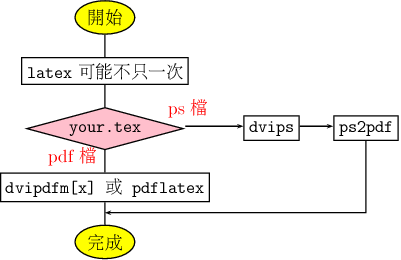
\includegraphics{latex-flow}
\end{center}

\section{\LaTeX\ ���S���M�βŸ�}
�b \TeX/\LaTeX\ ���@�ɡA��l��Z���O�¤�r�ɡA����@�ؽs�边���i�H���}�ӽs��B�[�ݡC�ӱƪ����O�q�`�O�Ѥϱ׽u�]\textbackslash, backslash�^\index{�ϱ׽u}\index{backslash}�Ҷ}�Y�Ӥ޾ɡC����\index{����}�h�O�Ѧʤ����]\texttt{\%}�^�Ӥ޾ɡC�Ҧp�A�H�s�边�s��U�C��r�G

\begin{quote}
\begin{verbatim}
This is my first \LaTeX\ typesetting example.
\end{verbatim}
\end{quote}

�sĶ��|�ܦ��H�U�����G�G

\begin{quote}
This is my first \LaTeX\ typesetting example.
\end{quote}

�䤤�� \verb|\LaTeX| �N�O \LaTeX\ ���@�ӫ��O�A�|��� \LaTeX\ �o�ӯS�����ϥܡC

�ѩ�A����a���y�t�A�q�`�r���B�Ÿ����̤j�e�q�u�� 256 �ӡ]$2^8$�^�A�]���A�\�h�{�����Ÿ��������ӷ���������O�A�~��ŦX�ƪ����h�ˤƻݨD�C�H�U���Ÿ��A��IJ \TeX/\LaTeX\ ���B�͡A�i�ೣ�o�ɮɯd�N�A���n���g�B�z�N�����g�i��Z���Y�h�F�C

�q�`�A�s�边���y�k�C��\index{�y�k�C��}�|���U�P�_�y�k�O�_���T�A�����O���৹���L�ʡA�����٬O�|�|���A�o�ɧO�ѤF�d�ݤ@�U {\tt *.log} �ɮסA�Ҧp�G�sĶ {\tt your.tex} �ɪ��ܡA�L�� log �ɴN�O {\tt your.log}�C

\begin{quote}
\begin{tabular}{llll}
�Ÿ� & �@�� & ��Z�W�ϥ� & \LaTeX\ �����N���O \\
\hline
\textbackslash & �U�ƪ��R�O & \verb|$\backslash$| & \verb|\textbackslash|\\
\%             & ����       & \verb|\%|           & NA \\
\#             & �w�q����   & \verb|\#|           & NA \\
\~{}           & ���ͤ@�Ӫť�   & \verb|\~{}|     & \verb|\textasciitilde| \\
\$             & �i�J�]���}�^�ƾǼҦ� & \verb|\$| & \verb|\textdollar| \\
\_{}           & �ƾǼҦ������ͤU�Цr & \verb|\_{}| & \verb|\textunderscore| \\
\^{}           & �ƾǼҦ������ͤW�Цr & \verb|\^{}| & \verb|\textasciicircum| \\
\{     & �ХܩR�O���@�νd��   & \verb|\{| & \verb|\textbraceleft|\\
\}     & �ХܩR�O���@�νd��   & \verb|\}| & \verb|\textbraceright|\\
\textless      & �ƾǼҦ������p��Ÿ� & \verb|$<$| & \verb|\textless| \\
\textgreater & �ƾǼҦ������j��Ÿ�   & \verb|$>$| & \verb|\textgreater| \\
\textbar     & OT1 �s�X�A�ƾǼҦ����~�ॿ�T��� & \verb+$|$+ & \verb|\textbar| \\
\&           & ���椤�����j�Ÿ�   & \verb|\&| & NA
\end{tabular}
\end{quote}

\section{\LaTeX\ �ƪ��W���@�dzW�d�κD��}
\label{sec:convention}\index{�W�d}\index{�D��}

���F�W���ҽͨ쪺�S���Ÿ��~�A�]���@�dzW�d�κD�ҭn���u�A���ǬO����w�ʪ��W�w�A���ǫh�u�O�D�ҡA�i�ण�P����a�B�y���|�����P���D�ҡA�Ȯɥ���L�����O \LaTeX\ ���C���W�h\index{�C���W�h}�N���F�C

\subsection{�r���������N�y}
\label{subsec:baseline}

�n�ͱƪ��W���W�d�B�D�ҫe�A�ڭ̱o���{�Ѥ@�U�r�����@�dzN�y�A�H�K����峹������ɦ��ӷ����C�q�`�ڭ̨C�Ӧr���O�m���@�Ӱ��Q����ؤ��A�٬� em-square\index{em-square}�A�P�@�Ӧr�����P�@���I�ơA�C�@�� em-square �j�p���O�ۦP���A��ڤW���r�]glyph\index{glyph}�^�n�m��b�o�� em-square �������m�A�o�O�r���]�p�̪��[�I�A�ҥH�A�P���I�ƪ����P�r���A�L���r���j�p���@�w�|�@�ˡA�]���ڭ̬O�ϥ� em-square ���j�p�b������A�ӫD��ڪ� glyph�C

�b�峹���ƦC���ɭԡA�h�O�N glyph �m��@�ӥH���Q�Ѧ��I�]reference point�^\index{���Q�Ѧ��I}\index{reference point}����Ǫ��@�Ӱ��Q�u�W�A�٬���u�]baseline\index{��u}\index{baseline}�^�A�j�g�r�����F Q �H�~�A�L�̪��������O�m���u�W���C���p�g�r���h���@�w��n�y���b��u�W�A���Ǧr�����e�i��W�X��u�H�U�A�Ҧp y�Bj ���r���C����r���b�峹�����m���m�A�ڭ̨Ӭݬݤ@�Ӽ����ϡG\footnote{��ڦr���]�p�W���U�����M���W���ε��c�A���M���|�O�o��²���A�o�̪������ϡA�u�O�Ȯ����r���@��m�񦳭Ӳʲ��������C}

% looks ugly, but l2h cannot handle this MP file be transparent png.
\begin{center}
\latexhtml{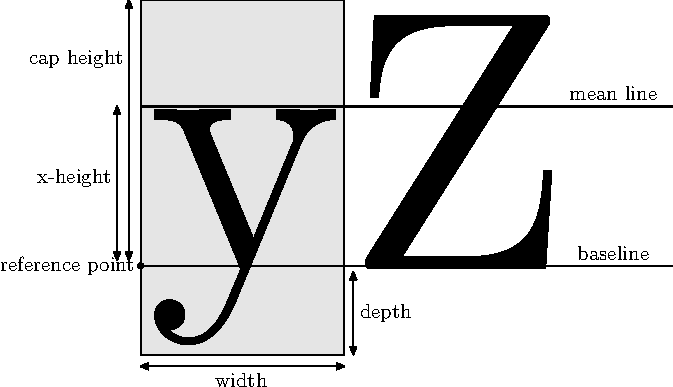
\includegraphics{baseline.1}}{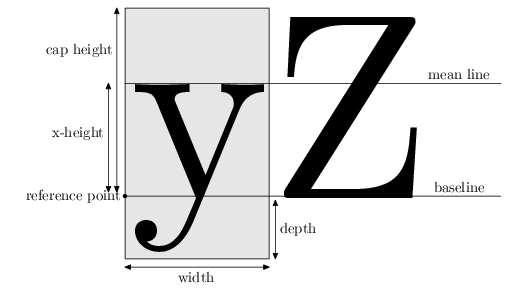
\includegraphics{baseline}}
\end{center}

�o�ӶW�X��u�H�U�����סA�ڭ̺٤����`�ס]depth\index{�`��}\index{depth}�^�A�H�W���N�٬��r���]height\index{�r��}\index{height}�^�A���M�j�p�g�����P�S�����j�g�r�����r���]cap height\index{cap height}�^�Τp�g�r�� x ���r���]x-height\index{x-height}�^�A�ѩ�o�ӨҤl�̬O�զX�r\index{�զX�r}�A�ҥH�C�Ӧr���e�ס]width\index{�e��}\index{width}�^���@�w�|�@�ˡA�����r���r�ڪ��h�O���e���r���C�r���[�W�`�סA�ڭ̴N�٤��� totalheight\index{totalheight}�A�j���������p�A�ȶȻ� height �ɬO���]�A depth ���A�ӥB�q�`�����O cap height�C

mean line\index{mean line} �b�@�����֥Ψ�A�q�`�O�r���]�p\index{�r���]�p}�ɤ~�|�Ψ�A�L�O���p�g�r���h���W����X�������ҳs�����@�Ӱ�ǽu�A�o�� mean line �� baseline ���Z���A�@��N�٬� x-height�A���M�N�O�p�g�r�� x �����סA�]���ڭ̷|���@�Ӫ��׳��A�٬� ex�A�����N�O�o�� x-height�C

����r���ܤ���S���A�L�O�H em-square �������I�Ӹm�� glyph ���A�b���^��V�X�ɡA����r�ä��O��n�y�����u�W���A�|�W�X��u�U�@�I�I�A�ܩ�|�W�X�h�֡A�h�M�r�����]�p�����A�C�ئr�������i��|���P�C�o�]�O���D�ƪ��W���@�P�ʡA�r���i�ೣ�ݭn�ɶq�ϥΦP�@�M���U�ئr������]�A�_�h�N�o�g�L�L�աA�~��Ͼ�Ӧr�����{�W���o��դ@�P�C

�o�DZM���N�y�A���ᴣ��@�ǫ��O���Ѽƪ��y�z�ɳ��|�ϥΨ�A�]�������x�@�U�A�Ҧp�G�r�������\index{�r������}�A��ڪ��N�O�H�Ѧ��I�]reference point�^���ǡA�u�����X���b�ߨӱ��઺�A�Ӥ@��һ�����Z\index{��Z}�A�����O�W�U�� baseline ���Z���C

\subsection{�@��ʪ��C���W�h}
\label{gen:gamerules}\index{�C���W�h}

\begin{enumerate}
\item \LaTeX\ �����O���O�j�p�g���O���A�� \verb|\| �}�Y�A�ᱵ�Ѧr���զ����r��γ�@���D�r���r���C�䤤�� \verb|[ ]| ���A���A�����O��ܩʰѼ�\index{��ܩʰѼ�}�A�i�H�ٲ��A�� \verb|{ }| �j�A���A�����O����ٲ����ѼơA���M�A\LaTeX\ �����O���@�w�|���ѼơA�����j�������|���ѼơA�u���L��L���ٲ��ϥιw�]�Ƚ}�F�C

\item \LaTeX\ ��Z���A�Ť@�ӭ^��ťթM�Ŧh�ӭ^��ťժ��@�άO�@�ˡA\LaTeX\ �|�{�@�@�ӭ^��ťաC

\item ���`�ڭ̽s��¤�r�ɡA���� \textsf{Enter} ��A�N�N������A����ڱƪ��X�ӡA�@�檺�e�׬O���ӱƪ��������]�w�A�]�N�O���A�A�b��Z���� \textsf{Enter}�A���N���ƪ���N�O�q�o���_��\index{�_��}�A\LaTeX\ �|�̤@���������e�׸g�L����p���۰ʸɦ��@����A���_��A�ӥB�|�b�����۰ʸɨ��@�ӪťաC�o�b�^��ܦ۵M�A�٬��r�]word�^���ť�\index{�r���ť�}�A������h���@�ˡA�b�s�边���s�褤��A�H�N�� \textsf{Enter} �����G�A�|�y���峹�������嶡�X�{�ťաC�o�|�b���夤�A�����ɾ��A���X�ѨM����k�C

\item �s�边���A�h���X�� \textsf{Enter} �N�h�ťX�X��A���b \LaTeX\ ��Z�̡A�h�Ӫťզ�\index{�ťզ�}�A�M�@�Ӫťզ�O�@�˪��@�ΡA\LaTeX\ �|��L�{�@�O�@�Ӫťզ�C�ӳo�Ӫťզ�A\LaTeX\ �P�ɤ]�|�{�@�O�s�q�����}�l�A�ҥH \LaTeX\ �O�H�ťզ�Ӥ��j�U�Ӭq���C

\item \LaTeX\ �w�]�C�ӳ��`���Ĥ@�Ӭq�����Ĥ@��O�����Y�]noindent\index{�����Y}\index{noindent}�^�A�q�ĤG�Ӭq���}�l�~�|���Y�]indent\index{���Y}\index{indent}�^�C���M�A�o�O�i�H��諸�A����|�A���ΡC

\item \LaTeX\ �����O�A�O�q�ϱ׽u\index{�ϱ׽u}��Ĥ@�Ӧr���}�l�A��Ĥ@�ӫD�r���Ÿ�����]�]�A�ťաB���I�Ÿ��μƦr�^�C�]���G

\begin{quote}
\begin{verbatim}
This is my first \LaTeX typesetting example.
\end{verbatim}
\end{quote}

�o�˪��ܡA��ڵ��G�A�]�� \verb|\LaTeX| �᪺�ťլO�ݩ���O���@�����A�ťձN���|�Q�����A�o�˷|�L���G

\begin{quote}
This is my first \LaTeX typesetting example.
\end{quote}

�o�ص��G�A\LaTeX\ �M typesetting �s�b�@�_�F�C�n�קK���ܡA�N�n���w���O���@�νd��A�Ҧp�H�U���j�A���C�δN�u���[�ӪťաA�Ҧp \verb|\ |�A\LaTeX\ �I�� \verb|\| �N�|�Φ����㪺���O�A��᪺�ťմN�|�Q�u���������ťդF�G

\begin{quote}
\begin{verbatim}
This is my first {\LaTeX} typesetting example.
This is my first \LaTeX{} typesetting example.
This is my first \LaTeX\ typesetting example.
\end{verbatim}
\end{quote}

�ҥH�A���`�L�X�����ӬO�G

\begin{quote}
This is my first \LaTeX\ typesetting example.
\end{quote}

\item ���ѲŸ��]{\tt \%}�^\index{���ѲŸ�}\index{%@\verb=%=}�A�i�H��b�@�檺����a��A{\tt \%} �᪺��r�|�Q \LaTeX\ �����C�ҥH�A�p�G�O��b�@�檺�̧��ݡA���� \LaTeX\ �|�۰ʴ��J���r���ťդ]�N�|�Q�����C�Ҧp�G

\begin{quote}
\begin{verbatim}
This is my fisrt \LaTeX\ document. Give \LaTeX\ a%
try.
\end{verbatim}
\end{quote}

�o�ˤ@�ӡA�ƪ��X�ӷ|�ܦ��G

\begin{quote}
This is my fisrt \LaTeX\ document. Give \LaTeX\ a%
try.
\end{quote}

a �M try �s�b�@�_�F�I���`���ӬO�G

\begin{quote}
This is my fisrt \LaTeX\ document. Give \LaTeX\ a try.
\end{quote}

���o�ӯS�ʡA�ڭ̥i�H���Φb����A�]�N�O���b�s�边\index{�s�边}���A����峹�� \textsf{Enter} �䴫��ɡA���ݥ[�� {\tt \%}�A�o�ˤ@�� \LaTeX\ �N���|���J�^��r���ťաA����r�N�i�H�s�������S���ťժ��@���F�A�_�h \LaTeX\ �b��g��Z�_�y\index{�_�y}�ɡA�|�۰ʦb�촫��B��J�@�ӭ^��ťաA�]���A��l�� \TeX/\LaTeX\ �O�{���o���媺�C

\item ���^��V�X���ɭԡA�q�`�A�^��r�e�᳣�|�d�ӪťաA�H�K�M����Ϲj�}�ӡA�u�O�o�Ӫťխn�h�j�A�o�N�S���T�w���D�ҡA�q�`�d�ӭ^��ťդ]�O�i�H�A�n���s���ܡA���ͨ줤��ƪ�����ij�D�ɦA�ӰQ�סA�ثe�N�i���ߺD�A�^���r�e��d�ӭ^��ťաC
\end{enumerate}


\subsection{�w����I�Ÿ����C���W�h}

\begin{enumerate}
\item ���^�媺�޸�\index{�޸�}���@�ˡA�o�̽ЯS�O�`�N�A�\�h�H�`�`�d���C���B�^��޸����޳������n�����k�C�^�媺�ܡA���䪺�޸��O grave accent�A�O��L���W�� {\sf Esc} �� {\sf F1} �U�観�i�θ������@����F�k�䪺�O apostrophe\index{apostrophe}�A�]�N�O��L���� {\sf Enter} ��j����������C���޸������άO��J�⦸������޸�\index{����޸�}�Ψ⦸���k��޸�\index{�k��޸�}�A�Ӥ��O�� \verb|"| �o�Ӥ@����������I�� ditto marks\index{ditto marks}�C�ҥH�A��ڤW�b��J��Z�ɬO�G

\begin{quote}
\begin{verbatim}
Please press an `Esc' key.
Please press an 'Esc' key. �o�O���~�ܽd�I
``This sentence.''
"This sentence." �o�O���~�ܽd�I
\end{verbatim}
\end{quote}

�ƪ��X�Ӫ����άO�G

%begin{latexonly}
\begin{quote}
Please press an `Esc' key.\\
Please press an 'Esc' key. �o�O���~�ܽd�I\\
``This sentence.''\\
"This sentence." �o�O���~�ܽd�I
\end{quote}
%end{latexonly}

\begin{htmlonly}
\begin{quote}
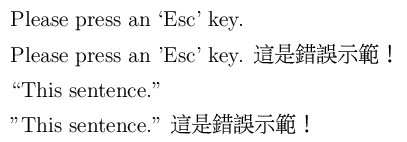
\includegraphics{quotation}
\end{quote}
\end{htmlonly}


���媺�ܡA�ڭ̬O�ϥΤ�����Ϊ��u�B�v�Ρy�B�z�A�b����j���h�w��ΩM�^��ۦP�Ϊ������βŸ��A���o�b���媽�Ʈɷ|�X���D�A�]���A���媺��B���޸��٬O�o�����ڭ̥ثe�ϥΪ��C

\item \LaTeX\ �|�b�^��峹���@�ӥy�l�����M�t�@�ӥy�l�}�l�������A�۰ʽվ㦨���j�@�I���ťաA�o�i�H�W�[�峹����Ū�ʡC�ҿפ@�ӥy�l�����A�Ҧp�G�y�I�].�^�B�ݸ��]?�^�B��ĸ��]!�^�Ϋ_���]:�^�A�o���M�O���^�媺�b�μ��I�Ÿ��A���O���媺���μ��I�Ÿ��C�A�i�H�`�N�@�U�W�����|���Ҥl�A�b document.\ �M Give �������ťշ|�y�L�j���L�^���r�����ťաC

�{�b�����D�O�A�p�G�o�Ǽ��I�Ÿ��᭱���O�t�@�ӥy�l���}�l���ɭԡA\LaTeX\ �L�k�h�P�_�o�ر��ΡA�o�ɱo�ѧڭ̦ۤv�ۦ�P�_�B�B�z�F�C�Ҧp�^���Y�g�r�G

\begin{quote}
\begin{verbatim}
I am Mr. Edward G.J. Lee, G.J. is a abbreviation of my name.
I am Mr.~Edward G.J. Lee, G.J. is a abbreviation of my name.
I am Mr.\ Edward G.J. Lee, G.J. is a abbreviation of my name.
\end{verbatim}
\end{quote}

�䤤 \verb|Mr.\ Edward| ���g�k�A�M \verb|Mr.~Edward| �X�G�O�@�˪��A���O�j�����J�@�Ӥ���p�����`��r���ť�\index{��r���ť�}�A�t�O�b���̤]�t�~���ܤ��i�H�q�o�̴���A�q�`�Φb�H�W���ɭԡA���L�̤��P���_�A�@��b�H�W���ƪ��A�]�A�L���Y�ΡB¾�١A�O�����_�����Ӥ��}���C�ӥB��Ӥ�y�������ܡA�H��̸�����A�~���|�]���_��Q������b�A�o�� {\tt ~} �Ÿ��]�]���b \TeX\ ���M���W���A�N�٬� tie\index{tie}�A��L�̸j�����N��C�ƪ��X�Ӫ��ɭԷ|�ܦ��G

%begin{latexonly}
\begin{quote}
I am Mr. Edward G.J. Lee, G.J. is an abbreviation of my name.\\
I am Mr.\ Edward G.J. Lee, G.J. is an abbreviation of my name.
\end{quote}
%end{latexonly}

\begin{htmlonly}
\begin{quote}
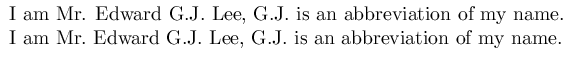
\includegraphics{abbreviation}
\end{quote}
\end{htmlonly}

�Щ�j�h�J�Ӥ���@�U���G�N���D�F�C�ĤG�檺�~�O���T���AMr.\ �M Edward �������ťլO���`��r���ťաA��Ĥ@�檺�y�l�����ťխn�p�@�I�I�C��L���ϥΨ��Y�g�r�����X�A�Ҧp�G`Dr.'�B`etc.'�B`e.g.'�B`i.e.'�B`vs.'�B`Fig.'�B`cf.'�B`Mrs.'�A�o�dz����O�N���y�l�����A�ҥH�A�n���J�@�ӥ��`�ťաC

�� G.J. �᭱������S�����J���`�ťաH���O�]���AJ �O�j�g���A�o�� \LaTeX\ ���|�h�~�{���O�y�l�����A�q�`�y�l�����ɪ��y�I�e�����Ӧr���O�p�g���CWell�A���S��ı�o���I�D�z�H:-)

�����A�Ʊ��٨S�������IKnuth �б¥X�F�@�D���D�A�p�G�y�l�������O `Please see Appendix A.' �᭱�S�ٱ����t�@�ӥy�l�C�o�ɫ���H�ѩ�A���|�{���O�y�l�����A�]���|���J���`�ťաA���o���O�y�l�����r�I�мȮɥ��O�o�A�ϥ� \verb|...Appendix A\null.|�A�� \verb|...Appendix A\@.|�C�o�ӻ��Ӧ��I�ܪ��A�����|�A�ӱ��Q�A�аO�o `\verb|\null|' �M�y�I���O�S���ťժ��C�Ҧp�G

\begin{quote}
\begin{verbatim}
Please see Appendix A. We will be there soon.
Please see Appendix A\null. We will be there soon.
\end{verbatim}
\end{quote}

�ƪ��X�Ӫ����G�N�|�O�]�t��������A�Фp�ߤ���^�G

%begin{latexonly}
\begin{quote}
Please see Appendix A. We will be there soon.\\
Please see Appendix A\null. We will be there soon.
\end{quote}
%end{latexonly}

\begin{htmlonly}
\begin{quote}
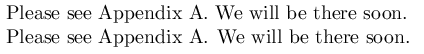
\includegraphics{abbreviation2}
\end{quote}
\end{htmlonly}

�p�G�A�A�{�b�\Ū���O HTML\index{HTML} �榡���A���ǨҤl�p�G�L�k������ܥX�ӡA�Ч�\�� PDF �����C�ӥB�A�p�G�A�s�@ PDF �榡�ɡA�r���S�����O�]���媺�^�Ʀr�O�O�J Computer Modern Type1 �r���^�A�t���i��N�|�󤣩���C�i�յۨϥ� {\sf gv/gsview}\index{gv@\textsf{gs}}\index{gview@\textsf{gview}} �h�\���A�M��վ㦨 Landscape\index{Landscape}�A��y�l�����Ԩ���t���a��h�N�ݱo�X�ӤF�C�o�b�y�l�h���ɭԡA�o�Ӫťդ]�ëD�T�w�j�p���A\LaTeX\ �|���峹���c���ݭn���ӷL���վ�C

\item �R�`��\index{�R�`��}����^�]�O���P�A�^��O�T�I�A�p�G�I��y�I���ܡA�h�O�|�I�C���媺�ܬO���I�A�I�줤��y�I�ܮe���N���o�M���C���O�^��o�ӤT�I�A���O�N���ӤT�ӥy�I�F�ơA�o�˪��I�ӱK���A�i�H�ϥ� \verb|\ldots| �� \verb|\dots| ���O�A�Ҧp�G

\begin{quote}
\begin{verbatim}
I'm not a good man ..., but a good husband .... ���~�ܽd�I
I'm not a good \ldots\ man \ldots, but a good husband \ldots.
I'm not a good \dots\ man \dots, but a good husband \dots.
\end{verbatim}
\end{quote}

�ƪ��X���ӵ��G�O�G

%begin{latexonly}
\begin{quote}
I'm not a good ... man ..., but a good husband .... ���~�ܽd�I\\
I'm not a good \ldots\ man \ldots, but a good husband \ldots.\\
I'm not a good \dots\ man \dots, but a good husband \ldots.
\end{quote}
%end{latexonly}

\begin{htmlonly}
\begin{quote}
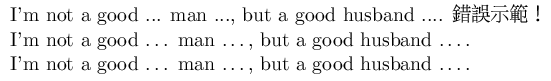
\includegraphics{dots}
\end{quote}
\end{htmlonly}

���媺�R�`���O�Ѩ�ӥ��Ϊ��T�I�Ҳզ����I���A�Y�G\chdots{}�A�N�O�ڭ� Big-5 �X�� {\tt 0xa14b}�]{\tt U+2026}�^�A���ѩ� Unicode\index{Unicode} �|���@�� MIDLINE HORIZONTAL ELLIPSIS({\tt U+22EF})�A�]���A���dzn��b��Ū�W���i��|���@�ˡA�]���ڭ̪��r���A�j�����b�s�@���I�Ÿ��ɬO�m�b�������a��A��������j���O�m��b��u���a��A�� Unicode �x��ĥΪ��˥��r���A��n�O����j�����t�өҴ��ѡA�o�ˤ@�Ӧ��dzn��u�@�̴N�{���ڭ̪��R�`�����ӬO {\tt U+22EF} �F�A�ܤ������A�ڭ̪� Big-5\index{Big-5} �X�èS���۹������r�X�C

\item �}�鸹\index{�}�鸹}�C�b�^��A�۷���}�鸹���i�঳�T�ءG
  \begin{itemize}
    \item hyphen\index{hyphen}\\
�o�O�̵u�� dash\index{dash}�A�q�`�N�O��J \verb|-| �N��F�A�Ҧp \verb|father-in-low|�A�o�˷|���{�� fater-in-low�C
    \item en-dash\index{en-dash}\\
�o�O�̱`�Ϊ��}�鸹�A�O��J��� hyphen�C�Ҧp \verb|1991--2003 �~|�A�o�|���{�� 1991--2003 �~�C
    \item em-dash\index{em-dash}\\
�o�O�̪��� dash�A�ѤT�ӳs�� hyphen �զ��A���ӬO�̬۪��ڭ̤���һ����}�鸹�C�Ҧp \verb|I am---a good man.| �|���{�� I am---a good man.�C�ܩ�o�ӤT�ӳs�� hyphen �e��O�_�n�d�ťաA�����H�ϥΡA�èS���w�ʪ��D�ҡA�����F�M���媺�}�鸹�t�X�]����}�鸹�e��A�q�`���d�ťա^�A�ӤH�q�`�O���d�ťժ��C
    \item �u�����\\
�o�������O�}�鸹�A�ӬO��ڪ���έt���A�o�n�i�J�ƾǼҦ��A�Ҧp�G�t���A�n�g�� \verb|$-5$|�A�M����{�X�ӬO $-5$�C�o�]�`�`�|���H�d���A���ઽ����J�@�몺�t��������ӥR�ơA�o�O�]�� \TeX/\LaTeX\ ���ƾǦ��l���Φr�M���j�B�z�A�M�@�뤺�夣�P�����Y�C
    \item ���媺�}�鸹\\
���媺�}�鸹�O����Ӥ���r��m�����@��u�A���שM�R�`���ۦP�C�b���u��m���A�w�q�W�O����ءAen-dash �O {\tt Big-5 0xa156}�Aem-dash �O {\tt Big-5 0xa158}�C���ѩ󤤤�r���Z�����D�A���i�ॴ�X�Ӫ��}�鸹�����|���@�I�ť�\footnote{�o�O�i�H�վ㪺�A�]�N�O�h����Ӿ�u�������r���Z�A�o�˴N���|���ͤp�ťդF�A����R�`���]���P�˪����ΡA�ڭ̷|�b�L�ժ������A�ӰQ�סC}�A�Ҧp�X�X���媺 em-dash�A�o�O�V�V���媺 en-dash�C�b�פ夤�A�}�鸹�q�`�i�H�ϥΤp�A���Ϋ_���N���C
    \item ���媺�p�W���ήѦW��\\
���媺�p�W��\index{�p�W��}�A�i�H�Щ��H�W�B�a�W�A�p\underline{�]�h�P}�F�ѦW��\index{�ѦW��}�]�p�W�������u�����i���Ϊ��^�A�i�H�Φb�ѦW�A�o�DzŸ��`�y���ƪ��W���x�Z�A�`�ϥ� �m �n�Ө��N�ѦW���A�p�W���h�L��L���N��k�C�b�@�몺�۵M�����ά�ǽפ�W�q�`���ϥγo���¦����p�W���ήѦW���C
\end{itemize}

\item ���Y�I\index{���Y�I}\\
�o�i�O�ƪ������n�\��C�^�媺�q�`�S�����D�A\LaTeX\ �|�۰��׶}�B�z�A����N���@�w�F�A\LaTeX\ �i���{�Ѥ���A���q�`��������{���ήM��A�h�h�ֳ֤��|�B�z�A�u���L�A���ɭ԰����i��|�~�P�C����A�쩳����O���Y�I�H���U�C�Ӫ��A�j�a�N���դF�A�ڦC���媺�A�^�媺�N���C�X�ӤF�A�]�� \LaTeX\ �|�۰ʳB�z�A�����ڭ̾�ߡC

\begin{quote}
\begin{tabular}{ll}
���I�Ÿ� & �m��B\\
\hline
�A�C�F�B:�v�^�n�I�H & ����m��歺\\
�u�]�m              & ����m����\\
�}�鸹�ΧR�`��      & �m�󭺧��ҥi\\
\end{tabular}
\end{quote}

²�檺���A���F�}�鸹�ΧR�`���A�S���}�f���A����m��̶}�Y�A�}�f�V�k���A����m��̥k�A�}�f�V�����A����m��̥��C�q�`���|�B�z�n�A���սZ���ɭԭn�`�N�@�U�~�P���a��C
\end{enumerate}

\section{\LaTeX\ ����Z���c}
\label{sec:struct}\index{��Z���c}

\subsection{���ҡ]environment�^\index{����}\index{environment}}

�W�@�`�ҽͪ����O���O�A���M�]�i�H�Ѥj�A��\index{�j�A��}�өw�@�νd��A���p�G�O�@��q�A�ƦܬO�@��g�峹���n�@�ήɡA�����O�i��N���ܾA�X�F�A�]���A\LaTeX\ �]���@�إ������c�A�٬����ҡ]environment�^�A�D�n�O���@�νd����X�j�ܸ��j���d��C

�Ҧ������ҡA���O�_�� \verb|\begin{���ҦW��}|�A��� \verb|\end{���ҦW��}|�A�o��ӫ��O��������Z���|�Q�@�ΡA�ӥB�A���Ҥ����٥i�H�M�Ψ�L���P�����ҡC

\LaTeX\ ��Z������A���N�O�]�b�@�� \verb|\begin{document}| �M \verb|\end{document}| �o�� document ���ҷ����C

\subsection{��²�檺 \LaTeX\ ����Z���c}

�H�U�N�O�Ҧ� \LaTeX\ ���ݨ�ƪ���Z�j���c�G

\begin{quote}
\begin{verbatim}
\documentclass{article}

  �o�̬O preamble ��

\begin{document}

  �o�̬O�����

\end{document}
\end{verbatim}
\end{quote}

\verb|\documentclass{article}|�A�o�O�b�i�D \LaTeX\ �ϥέ��@�����O�A�ڭ̥ثe�ϥΪ��O {\tt article} ���O\index{���O}\index{article}�A�������O�|�b�� \ref{ch:class} ���Q�סCpreamble\index{preamble} �ϡA�h�O�U�@�Ƿ|�v�T��Ӥ�Z�����O�A�ΤޥΥ����M�󪺦a��A���M�A�������ޥΥ����A�]���ϥμv�T���媺���O���ܡApreamble �ϴN�O�ťաA���g����F��C����ϡA�N�O�ڭ̹�ڤW�g�峹���a��C

�{�b�]�i�H��e�����|���Ҥl�A��J����ϸ��Y�Apreamble �ϪťըS���Y�A�M��s�ɡA�յ۽sĶ�ݬݡG

\begin{quote}
\begin{verbatim}
latex example.tex
dvips example.dvi      => ���� ps �榡 example.ps
dvipdfm[x] example.dvi => ���� pdf �榡
pdflatex example.tex   => ������ .tex ���� .pdf
\end{verbatim}
\end{quote}

�u������Ҹѻ��A�|�b�U�@���Ӷi��A�ҥH�A�o�̼Ȯɤ��|���Ц��������ҥi�H�ϥΡA�����ݬݨS�����Y�C�ѩ��٨S�ͨ줤�媺���D�A�]���p�G�A�Q�ոլݡA���Ȯɥ��ϥέ^��A�D�z���O�۳q���C

\subsection{preamble �ϥi�H��Ǥ���H}
\label{subsec:preamble}

�o�̥i�H�ޥΥ����A�ӥB�|�v�T��g��Z�����O�A�Ҧp�@�Ǩƥ��w�q�n�����O�A�Q�b��g��Z���ϥΡA�N�i�H�m��b preamble �ϡC

\subsubsection{�������ޥ�}
\label{subsubsec:package}

����D�n�O�з� \LaTeX�A���e���w����A�|���ǥ����M�󤣱o���n�ޥΡA���U�N�ӻ����p��ޥήM��C�o�ǮM�󳣬O�@�� \TeX\ �t�γ��|���W���C

���O�����ҭn�p��}�Y�����йL�F�A�{�b�ӬݬݤޥΥ����n���}�Y�C

\begin{quote}
\begin{verbatim}
\documentclass{article}
\usepackage{color}
\begin{document}
\textcolor{blue}{This is blue color.}
\end{document}
\end{verbatim}
\end{quote}

�sĶ�@�U�A�ݬݵ��G�O����H�o�̨ϥΪ��N�O \textsf{color} package\index{color@\textsf{color}}�A���Y�O�� \TeX/\LaTeX\ macro �Ҽg���@�ӥ����M��C�@��²�檺�ڭ̴N�٬������]macro�^\index{����}\index{macro}�A�����@�I���N�٬������M��]package�^\index{�����M��}\index{package}�A���A���Y���O�@�˪��A�u���L�j�p�Φ��S����z���@�Өt�Ϊ��t�O�C

\LaTeX\ ���Y������{�����M��i�H�ϥΡA�C�Ӵ��G�� \TeX\ �t�ΩҦ������i�ೣ�|���Ҥ��P�C�j���S���H�i�H��q�Ҧ��{�s�� \LaTeX\ �����M��A�]����b�O�Ӧh�F�A���L�A����j�����|����`�Ϊ������M��C�ԲӪ������M�󪺺غءA�|�b�� \ref{ch:package} ���ӻ����C

\subsubsection{�v�T��g��Z�����O}

�|�v�T��g��Z�����O�A�q�`�]�O��b preamble �ϡA�Ҧp�G

\begin{quote}
\begin{verbatim}
\linespread{1.36}
\parindent=0pt
\end{verbatim}
\end{quote}

\verb|\linespread| �O�b����W�U�檺��Z�A�o�̴N�O�N��Z�ܦ���Ӫ� 1.36 ���C�ܩ󤰻�O��Z�O�H�N�O�o�@�檺��u�]baseline�^��U�@�檺��u���Z���A�q�`�^��峹�����h�վ�L����Z�A������o�A���[�j��Z�H�Q�\Ū�C

\verb|\parindent| �O�վ�q�����Y���{�סA�o�̽վ㦨 0�A�]�N�O���U�q���������Y���N��A�]�i�H�վ㦨��L���ȡA\LaTeX\ �N�|�̳o�ӭȥh���Y�C���M�A���h�]�w���ܡA\LaTeX\ �N�|�̥L���w�]�ȥh���Y�C


\subsection{���`���c\index{���`���c}}
\label{subsec:chapstruc}

����Ϸ��M�O�ڭ̼g�峹���D�n�a��A�Τ@�ǷL��\index{�L��}�C�b \LaTeX\ ����Z���Y�A���`���D���Φ����O�ѦP�˪����O�ӱ���A�o�˦��@�Ӧn�B�A�{�ɴ��J���`���D�Ψ䤺��ɡA�ڭ̤����h�z�|���D�s���Υؿ������D�A�]�����h�z�|�n�Τ���r���B�Φr���j�p�n�h�j�A\LaTeX\ �|�۰ʭp��B�z�A�r���j�p�]�|�M����ϥΪ��r���j�p���۰t�X�վ�A�ϥΪ̴N�M�ߦb����c��B�g�@�Y�i�C�H�U�ѦC�����A�Ѿ�ӳ��`���c�G

\begin{quote}
\begin{tabular}{lll}
�`�׼и� & ���O & �@�ΤΪ`�N�ƶ�\\
\hline
$-1$ & \verb|\part{}|          & �o�O�̤j�����c�A�ڭ̤���q�`�٬��u���v�C \\
0    & \verb|\chapter{}|       & ���C�b article ���O���Y�S�����C\\
1    & \verb|\section{}|       & �`�C\\
2    & \verb|\subsection{}|    & �p�`�C\\
3    & \verb|\subsubsection{}| & ���p�`�C\\
4    & \verb|\paragraph{}|     & �q���C\\
5    & \verb|\subparagraph{}|  & �p�q���C\\
\end{tabular}
\end{quote}

���`���D\index{���`���D}�����e�N�O�����g�J���O���j�A�����Y�N�i�H�F�A\LaTeX\ �b�ƪ��ɷ|�۰ʨϥβ���B�[�J���`�s��\index{���`�s��}�ίǤJ�ؿ�\index{�ؿ�}���Y�C

�ܩ�Ĥ@�檺�`�׼и��]secnumdepth�^\index{�`�׼и�}\index{secnumdepth}�A{\tt book/report}\index{book@\texttt{book}}\index{report@\texttt{report}} ���O���`�׼и��O 2�A{\tt article} ���O 3�C�o�O����N��O�H�N�O�� {\tt book/report} ���O����Z�A�b \verb|\subsection{}| �H��]{\tt subsection} �������|�s���^�A���`�N���A�s���F�F�P�˪��A�b {\tt article} ���O����Z�A�b \verb|\subsubsection{}| �H��N���s���F�C�����M�|�W�ߥX�@��W��Ӫ��ܳo�ӬO���D�C���s���F�����`���e�A���M�]�N���ǤJ�ؿ����Y�F�C�o���M�O�i�H��諸�A�u�n��� \LaTeX\ �� {\tt secnumdepth} �o���ܼƪ��ȴN�i�H�F�A�o�ө���|���Φp���� \LaTeX\ ���w�]�ȡC���o�g�峹�A�b preamble �ϴN���@�ӳ]�w�G

\begin{quote}
\begin{verbatim}
% let the depth of report to subsubsection
\setcounter{secnumdepth}{3}
\end{verbatim}
\end{quote}

�ҥH�A�o�g�峹���M�ϥΪ��O {\tt report} ���O�A���O���`���`�׼и��O�Цb 3�A�]�N�O���|�s���� {\tt subsubsection} ����A���o���M�O�S���s�J�ؿ������C 

�U�@���N���ڭ̶}�l��ڰʤ�a�I��\chdots{}�A����{�b���S�����㤶�Ы��O�O�H���ګ��|���D��������O�i�H�ϥΡH�o�O�]�� \LaTeX\ �����O�ܦh�A�������Ъ��ܡA�@�譱�O�����A�G�譱�]���e���A�ѥL����ڧ@�ΡA�ҥH�A�ڭ̱N�|�b�U���|�Үɬﴡ�b���Y�����A���o����󱵪���n�ɡA�A�Ӿ�z�ӫ��O�t�d���A�o�˥H��d���O�N�ܤ�K�F�A�����h���O�A�u�n���D���ӳo�˥\�઺���O�N���F�C


% ``�j�a�Ӿ� LaTeX'' LaTeX ��Z start.tex
% Copyright (c) 2004  Edward G.J. Lee <edt1023@info.sayya.org>
%
% �b���H�� GNU Free Documentation License 1.2 �ΥH�᪺�����W�d���U�A
% ���\�����B���G�έק�C���쪩�v�B���v�n�����o�����C
%
% �����G�����A�t�� fdl.tex�A���e�� GNU FDL ���W�d���C�p�G�򥢡A�i��
% http://www.gnu.org ���o�A�μg�H�ܦۥѳn�����|(Free Software Fundation)
% �����C
% 9 Temple Place - Suite 330, Boston, MA 02111-1307, USA.
%
% $Id: start.tex,v 1.38 2004/03/07 12:29:47 edt1023 Exp $
%
\chapter{��ڤW�ƪ����ݬ�}
\label{ch:start}

�n�F�A�{�b�����Ӫ��ݬݧa�I�����D�n�O²�檺��һ����A���i�J���p�A�ͨ�L�C������Τ񰪽���צ��Φh�F�C

���ӭӡu�̰����ɭ�h�v�G\textcolor{red}{\bf �Ƿ|����Ŷ��A�A�N�Ƿ|�ƪ��F}�I��DZƪ����B�͡A�����|��ҾǨ쪺�F��h�Q�k�l�G���A�Ҧ����Ŷ��]�N�O�@�ӭ����^�A����ڤW�A�A�n�վ㪺�A���O�U�ӳ������Ŷ��t�m�A��H�@�I���A�]�N�O�@��ӭ��������A�S����r�B�Ϫ��������~�O�ƪ��u�������I�C�A��ťť�N�n�A�L�@�q�ɶ������x��A�A�Ӧ^�Y��ҳo�ӡu���ˡv�Ŷ�����h�C:-)

�ѩ󥻤妳 HTML �����A���F�ഫ�W���y�����u�A��Ҫ������A��Z�W�u�g�{���X�A���G���������O�sĶ�n�� PDF �榡�ɮסA�m�������W�A�i�u�W�\���ΤU���A²�檺�Ҥl�h���t�s�@�W�ߪ� PDF �ɡA�аѾ\���媺 PDF �榡�ɮפ��e�C

\section{²�檺���}

�o�̴N��e�@���ҽͨ쪺�@�Ǥ��e��z���@�Ӥ�Z�A���ӸոլݡA�o�̥��ϥ� {\tt report}\index{report@\texttt{report}} ���O��Z�A�]�� {\tt article}\index{article@\texttt{article}} ���O��Z�O�S�� {\tt chapter} ���G

\begin{quote}
\begin{verbatim}
% example1.tex
\documentclass{report}
\begin{document}
This is my first {\LaTeX} typesetting example.\\
This is my first \LaTeX{} typesetting example.\\
This is my first \LaTeX\ typesetting example.\\
I am Mr. Edward G.J. Lee, G.J. is a abbreviation of my name.\\
I am Mr.\ Edward G.J. Lee, G.J. is a abbreviation of my name.\\
Please see Appendix A. We will be there soon.\\
Please see Appendix A\null. We will be there soon.
\end{document}
\end{verbatim}
\end{quote}

�ϥνs�边�s��A�M��s�ɦ� {\tt exmaple1.tex}�A�o�˴N�i�H�sĶ�F�G

\begin{quote}
\begin{verbatim}
latex example1.tex       => ���� example1.dvi
dvips -Ppdf example1.dvi => ���� example1.ps
ps2pdf example1.ps       => ���� example1.pdf ��
dvipdfm[x] example1.dvi  => �� example1.dvi �������� example1.pdf ��
pdflatex example1.tex    => �� example1.tex �������� example1.pdf
\end{verbatim}
\end{quote}

�sĶ�n�� PDF �ɥi�b���U���ξ\���G

\begin{quote}
\url{http://edt1023.sayya.org/tex/latex123/example1.tex}\\
\url{http://edt1023.sayya.org/tex/latex123/example1.pdf}
\end{quote}

\subsection{���󴫦�}
�C��̫�[�F�� \verb|\\|\index{\\@\verb=\\=}�A�o���ܱj�����檺�N��A�_�h \LaTeX\ �|�̪����w�]���e�רӴ���A�N���|�O�@�ӥy�l�@��F�A�j�a�i�H��o�� \verb|\\| �����A�A�ӽsĶ�լݬݵ��G�A�N�|���D���@�^�ƤF�C�]�i�H�ϥ� \verb|\newline|\index{newline@\verb=\newline=} �o�ӫ��O�A���M�A�ڭ̳��|�o������θ��u�����O�C�ӥB \verb|\\| �i�H�����ɪ����j�A�o�b \verb|\newline| �h����C�Ҧp�G

\begin{quote}
\begin{verbatim}
Please see Appendix A. We will be there soon.\\[1cm]
Please see Appendix A\null. We will be there soon.
\end{verbatim}
\end{quote}

�o�˪��ܡA��椧������Z\index{��Z}�N�O��Ӫ���Z�A�[�W {\tt 1cm}�C�ƦܡA�]�i�H�O�t�ƪ��ѼơA�o�˦�Z�N�|�ܦ���Ӫ���Z��h {\tt 1cm}�A���M�A�p�G�]�L�Y�F���ܡA���i��|���|�b�@�_�C�J�M�A�o�̨ϥΪ��O��A���A���ܳo�ǰѼƬO�i�H�ٲ����C

�t�~�A\verb|\linebreak[n]|\index{linebreak@\verb+\linebreak+} �]�i�H�j������\index{�j������}�A{\tt n} �N���� 1--4 ����ij�ȡA�ƭȷU�j���ܷU�O�j�P��ij�A���]�w���ܡA�N�O���Τ�����ؿ�ܡA�S�������a�a�C�M�e���һ������P�B�O�A�o�ش���|���Ө��@��y�l�����ץ������������W��e�����סC�Ҧp�G

\begin{quote}
\begin{verbatim}
Please see Appendix A. We will be there soon.\linebreak
Please see Appendix A\null. We will be there soon.
\end{verbatim}
\end{quote}

�ƪ���|���{���G

%begin{latexonly}
\begin{quote}
Please see Appendix A. We will be there soon.\linebreak
Please see Appendix A\null. We will be there soon.
\end{quote}
%end{latexonly}

\begin{htmlonly}
\begin{quote}
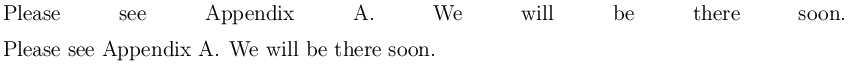
\includegraphics{linebreak}
\end{quote}
\end{htmlonly}

\subsection{�����Y��\index{�Y��}}

�Ĥ@���Y�ƤF�I�o�O�]���ڭ̧����S�������`�A�ҥH�A\LaTeX\ �N��o�Ǥ��e�����O�ި��������A�� \LaTeX\ ���w�ơA�ި��}�Y�O�|�Y�ƪ��C�n�ѨM�o�Ӱ��D�A�i����ؤ�k�G

\begin{enumerate}
\item �b�Ĥ@�椧�e�[�J \verb|\noindent|\index{noindent@\verb+\noindent+} �ӫ��� \LaTeX\ ���n�h�Y�ơC���O�o�u�@�Φb�U���O���a��A��L���Y�ƪ��a���٬O�|�Y�ơC
\item �b preamble �ϥ[�J \verb|\parindent=0pt|\index{parindent@\verb+\parindent+}�A�o���������媺�Y�Ƭ� {\tt 0pt}�A���M�A�o�N���ܥ��峣���n�Y�ƤF�C
\end{enumerate}

\section{�[�J���`���D\index{���`���D}}

�b \LaTeX\ ���Y�A�n�[�J���`���D��b�O�Ӯe���F�A�]�����h�ަr�骺�j�p�θm�񪺦�m�A�ɺޥ[�W�h�N��F�I\LaTeX\ �|���ڭ̦w�Ƥ@���C�ڭ̳o�̤��M�H {\tt report} ���O�ӻ����A�]�� {\tt article} ���O���Y�A�S�����A�u��A�Ω��²�檺�u��C

\begin{quote}
\begin{verbatim}
% example2.tex
\documentclass{report}
\begin{document}
This is the first experience of \LaTeX.
\chapter{Aesop Fables}
\section{The Ant and the Dove}

An ant went to the bank of a river to quench its thirst, and
being carried away by the rush of the stream, was on the
point of drowning.

A Dove sitting on a tree overhanging the water plucked a
leaf and let it fall into the stream close to her. The Ant
climbed onto it and floated in safety to the bank.

\section{The Dog in the Manger}

A dog lay in a manger, and by his growling and snapping
prevented the oxen from eating the hay which had been
placed for them.

``What a selfish Dog!'' said one of them to his companions;
``he cannot eat the hay himself, and yet refuses to allow
those to eat who can.''

\chapter{The Eagle and the Arrow}

An eagle sat on a lofty rock, watching the movements of a
Hare whom he sought to make his prey.

An archer, who saw the Eagle from a place of concealment,
took an accurate aim and wounded him mortally.
\end{document}
\end{verbatim}
\end{quote}

�sĶ�X�Ӫ����G�G

\begin{quote}
\url{http://edt1023.sayya.org/tex/latex123/example2.tex}\\
\url{http://edt1023.sayya.org/tex/latex123/example2.pdf}
\end{quote}

�Ъ`�N�L����ɭԷ|�Y�ơA����ɭԷ|�����C{\tt report} ���O�A�s���@���|�����A�p�G�Q�`�٤@�I�Ŷ��A�i�H���� {\tt article} ���O�A\verb|\chapter{}| ��� \verb|\section{}|�A��� \verb|\section{}| �N��� \verb|\subsection{}|�A�o�˴N���|�����A���e�N�|�s��U�h�F�C�j�a�i�H�յۧ� {\tt report} �令 {\tt article} �� {\tt book} �A���s�sĶ�@���A�ոլݵ��G���󤣦P�C

\section{�[�J title page ��T}
\label{sec:titlepage}\index{title page}

�o�O���������Ĥ@���A�ڤ]�����D�o�Ӥ���M���W���O����A�b \LaTeX\ ���Y�A�ڭ̴N�٬� title page�C�b \LaTeX\ ���зǮ榡�̡A�L�]�A�F���D�]title�^�B�@�̦W�r�]author�^�B����]date\index{date}�^�ηP�µ��]thanks\index{thanks}�^�C�n�`�N���O�A�b {\tt report/book} ���O�Atitle page �O�ۦ��@��W�����A���b {\tt article} ���O�̡A�L�O�M����s�_�Ӫ��C�ڭ̴N�H�W��������J�����峹���ҡA�n�ק諸�a��O preamble\index{preamble} �ϤΥ���Ϫ� \verb|\maketitle|\index{\verb=\maketitle=}�G

\begin{quote}
\begin{verbatim}
% example3.tex
\documentclass{report}
\title{Aesop Fables}
\author{Aesop\thanks{Thanks to the reader.}
       \and Nobody\thanks{Thanks to nobody.}}
\date{\today}
\begin{document}
\maketitle
This is the first experience of \LaTeX.
\chapter{Aesop Fables}
\section{The Ant and the Dove}
 ...
\end{verbatim}
\end{quote}

�ƪ��X�Ӫ����G�p�U�G

\begin{quote}
\url{http://edt1023.sayya.org/tex/latex123/example3.tex}\\
\url{http://edt1023.sayya.org/tex/latex123/example3.pdf}
\end{quote}

�ڭ̥i�H�o�{�A�o�@���O���s���X���A�q�U�@���}�l�~�O�Ĥ@���C�@�̥i�H���h�ӡA�ϥ� \verb|\and| ���O�ӳs���C������@�w�n���A�p�G�S�� \verb|\date{\today}| �o�ӫ��O�A���٬O������A���u��T�w�b���ѡC�p�G���e�L���A�L�|�۰ʧ��A���]�i�H��ʥ[ \verb|\\| �ӱj������A���ަp�󴫦�A��ӥy�l�O�~���ƦC���C\verb|\maketitle| �O�U�b����Ϫ��}�Y�A�p�G���U�o�ӫ��O�A���sĶ�ɤ��|��������~�A�u�O�N�S�� title page �F�C

\section{�[�J�ؿ��]Table of Contents�^}
\label{sec;toc}

�[�J�ؿ��]Table of Contents\index{Table of Contents}�^�� \LaTeX\ �Ө��A��O���ө��|���Ʊ��A�u�n�b����}�Y�[��
\verb=\tableofcontents=\index{tableofcontents@\verb=\tableofcontents=}
���O�N���F�I�̤W�����Ҥl�A�ק令�G

\begin{quote}
\begin{verbatim}
% example4.tex
\documentclass{report}
\title{Aesop Fables}
\author{Aesop\thanks{Thanks to the reader.}
       \and Nobody\thanks{Thanks to nobody}}
\date{\today}
\begin{document}
\maketitle
\tableofcontents
This is the first experience of \LaTeX.
\chapter{Aesop Fables}
\section{The Ant and the Dove}
 ...
\end{verbatim}
\end{quote}

�ƪ��X�Ӫ����G�p�U�G

\begin{quote}
\url{http://edt1023.sayya.org/tex/latex123/example4.tex}\\
\url{http://edt1023.sayya.org/tex/latex123/example4.pdf}
\end{quote}

�o�̤d�U�n�`�N���O�A\verb|\tableofcontents| �n�[�b \verb|\maketitle| ���᭱�A�_�h�ؿ��|�L�b title page ���e�C�ӥB�n\textcolor{red}{\bf �sĶ�⦸}�C�Ĥ@������ {\tt example4.toc}�A�M��ĤG���sĶ�A��ڳo�� {\tt toc} �ɡA�u���s�J�ؿ��C

�ؿ��O�]�A�Ϫ��ؿ����]List of Figures, List of Tables�^�A���ڭ̥ثe�٨S���ͨ�Ϫ����ƪ��A�]���Ȯɲ��L�A���ͨ�ɦA�Ӭݭn�p��[�J�Ϫ��ؿ��C

\section{�[�J�K�n�]abstract�^}
\label{sec:abstract}\index{abstract}

�o���@�w�|���A�p�G�n�[�J���ܡA�i�ϥ� {\tt abstract} ���ҡA�b�o�����Ҥ����峹�A���k�|�Y�ơC�n�`�N���O�A�u�� {\tt article/report} ���O�~�� abstract�A{\tt book} ���O����ϥγo�����ҡC

\begin{quote}
\begin{verbatim}
% example5.tex
\documentclass{report}
\title{Aesop Fables}
\author{Aesop\thanks{Thanks to the reader.}
       \and Nobody\thanks{Thanks to nobody}}
\date{\today}
\begin{document}
\maketitle
\begin{abstract}
The tale, the Parable, and the Fable are all common and popular
modes of conveying instruction. Each is distinguished by its own
special characteristics.
\end{abstract}
\tableofcontents
\chapter{Aesop Fables}
\section{The Ant and the Dove}
 ...
\end{verbatim}
\end{quote}

�ƪ��X�Ӫ����G�p�U�G

\begin{quote}
\url{http://edt1023.sayya.org/tex/latex123/example5.tex}\\
\url{http://edt1023.sayya.org/tex/latex123/example5.pdf}
\end{quote}

{\tt report}\index{\texttt{report}} ���O���K�n�ۦ��@���A���s���X�A�B���|�s�J�ؿ����A�o�M�@�몺�פ�榡�i��|���@�ˡA�ϥήɽЪ`�N�C{\tt artcile}\index{\texttt{artcile}} �����O�h���M�O�M����۳s���A�|�X�{�b�峹���D����C

{\tt abstract} �M summary\index{summary} �b���������פ�O���Ϥ����A�q�` abstract �b��e�Fsummary �h�b���C���ثe�@��ʪ��峹�h�S���o�˰ϧO�A�q�q�����u�K�n�v�C�q�`�A�K�n���Y�O���ε��ѡB�L�椬�ѷӤ]���ϥΤ����Ϫ����C


\section{�[�J����}
\label{sec:footnote}\index{����}

�b \LaTeX\ ���Y�A���ѥi����ؤ覡�A�@�جO�}���]footnote�^\index{footnote}\index{�}��}�A�@�جO����]marginal note�^\index{marginal note}\index{���}�C�q�` \LaTeX\ ���}���w�]�O�Ѫ��ԧB�Ʀr�b�s���A�m�󭶩����C�b�S�����]part�^�����ΤU�A\texttt{report/book} ���O�A�s���C���|�q�Y�_��A\texttt{article} ���O�h�|�s��A�ӥB�A�|�ϥ� \texttt{footnotesize}\index{footnotesize@\texttt{footnotesize}} ���r��L�X�C����h���s���A�r��O���`�j�p�C

\subsection{�}���]Footnote�^}

�b�ҭn�[�������Ӧr��A�ϥ� \verb|\footnote{}| ���O�Y�i�A�ѻ�����r�N�g�J�j�A�������A�@�� \LaTeX\ �����O�b�������M�����@�ΡA�|�L�b�����������A�H�p�@�I���r�ӦL�X�A�å[�W�s���C�H�U�ڭ̴N�ոլݦb Dove �o�Ӧr�Ӱ��}���C�Ъ`�N�ADove �o�Ӧr�M \verb|\footnote{}| �����O�S���ťժ��C

\begin{quote}
\begin{verbatim}
% example6.tex
\documentclass{report}
\title{Aesop Fables}
\author{Aesop\thanks{Thanks to the reader.}
       \and Nobody\thanks{Thanks to nobody}}
\date{\today}
\begin{document}
\maketitle
\tableofcontents
This is the first experience of \LaTeX.
\chapter{Aesop Fables}
\section{The Ant and the Dove}

An ant went to the bank of a river to quench its thirst, and
being carried away by the rush of the stream, was on the
point of drowning.

A Dove\footnote{Pigeon, an emblem of peace.}
sitting on a tree overhanging the water plucked a
leaf and let it fall into the stream close to her. The Ant
climbed onto it and floated in safety to the bank.
 ...
\end{verbatim}
\end{quote}

�ƪ��X�Ӫ����G�p�U�G

\begin{quote}
\url{http://edt1023.sayya.org/tex/latex123/example6.tex}\\
\url{http://edt1023.sayya.org/tex/latex123/example6.pdf}
\end{quote}

\subsection{����]Marginal note�^}

����u�O�� \verb|\footnote{}| ���� \verb|\marginpar{}|\index{marginpar@\verb=\marginpar=} �Ӥw�A���e���M�g�J�j�A�����C���M�}�����@�˪��O�A�L�S���s���]�]���N�b����A�L�����n�^�A�L���r��]���|�p�@���A�M���媺�r��j�p�O�@�˪��A�o�b�᭱�Q�ר�r�����ɭԷ|�ͨ�p����ܦr�骺�j�p�C

\begin{quote}
\begin{verbatim}
% example7.tex
\documentclass{report}
\title{Aesop Fables}
\author{Aesop\thanks{Thanks to the reader.}
       \and Nobody\thanks{Thanks to nobody}}
\date{\today}
\begin{document}
\maketitle
\tableofcontents
This is the first experience of \LaTeX.
\chapter{Aesop Fables}
\section{The Ant and the Dove}

An ant went to the bank of a river to quench its thirst, and
being carried away by the rush of the stream, was on the
point of drowning.

A Dove\marginpar{Pigeon, an emblem of peace.}
sitting on a tree overhanging the water plucked a
leaf and let it fall into the stream close to her. The Ant
climbed onto it and floated in safety to the bank.
 ...
\end{verbatim}
\end{quote}

�ƪ��X�Ӫ����G�p�U�G

\begin{quote}
\url{http://edt1023.sayya.org/tex/latex123/example7.tex}\\
\url{http://edt1023.sayya.org/tex/latex123/example7.pdf}
\end{quote}

\section{�r���������վ�}
\index{�r��!�����վ�}

\TeX/\LaTeX\ ���r���t�κ�O�۷��������A�o�̤��h�ͨ䤤��z�A���b�ϥΪ̪����סA�ڭ̥u�n���D���ϥδN��F�C�b�o�̡A�ڭ̻��r���]font�^\index{font}\index{�r��}�A�����O�r���������@���`�١A�κ٬��r��\index{�r��}�A�b�r���Ϊ����ɭԡA�ڭ̴N�٬��r�Ρ]font shape�^\index{font shape}\index{�r��}�C

\LaTeX\ �ϥΪ��r����r����A�H�ثe�s������ \LaTeX\ �Ө��A�O�ϥ� 1993 �~�o�檺 NFSS(New Font Selection Scheme) �ĤG�����зǡC���M�A���M�O�إߦb \TeX\ �r�������¦�W���A�o�w�W�X�o�g�峹���d��C

\subsection{\LaTeX\ ��r�����ݩʴy�z}
\label{subsec:font-attr}\index{�r��!�ݩʴy�z}

�b \LaTeX\ �̡A���r�����y�z�A�ϥΤF�����ݩʨӻ����A�o�����ݩʡA�]�O \LaTeX\ �������`�n�ϥΨ쪺�ѼơA�ƦܬO���~�T���Хܦr���ӷ����ɭԡA�|��r�����o���ݩʵ���ܥX�ӡC

\begin{enumerate}
\item �r���s�X�]font encoding�^\index{font encoding}\index{�r��!�r���s�X}\\
�o�̩ҿת��r���s�X�A�����O�U�ӭӧO���r�b�@�Ӧr�����Y���ƦC���ǤΦw�Ƥ覡�C��l�� \TeX\ �r���s�X�ڭ̴N�٬� OT1(Old \TeX\ text encoding)\index{OT1}�A�o�O�w�]���A�p�G�������w�r���s�X�A���ҨϥΪ��N�O OT1 �s�X�C�b�ثe�s�@�N���r���s�X���Y�A�r���w�Ƥ覡�Τ��e�M OT1 ���@�ˡA�Ҧp
T1\footnote{�����W�٬O Cork's \TeX\ extended text encoding �S�٬� Text Companion encoding�C�o�̪� T1 �M Type 1 �r���W��\index{�r��!�r���W��}�L���A�L�O�r���s�X�覡�A�L��r�����Y�����@�ǭ����Ÿ��r����W�����@�ӳ�W���r�A�ӫD�p OT1 �O�Ѥ@��r���M�����Ÿ��զX�Ӧ��C}\index{T1}�A�o�b���ᴣ����ܦr���s�X�ɷ|�A�ͨ�A�ڭ̥ثe�N���h�վ�r���s�X�A�ϥιw�]�� OT1�A��L���s�X�o�̴N���h�ͤF�C

\item �r�ڡ]font family�^\index{font family}\index{�r��}\\
���P�@�]�p�������r�����X���W�١A�Ҧpù���r�ڡ]roman�^\index{roman}\index{ù���r��}�B���r���r�ڡ]typewriter�^\index{typewriter}\index{���r���r��}�����A�q�`�e���|�a�W�s�@�өλs�@�H���W�١A�Ҧp Knuth\index{Knuth} �б³]�p���A�٬� `Computer Modern Roman'\index{Computer Modern Roman}�AAdobe ���q�s�@��ù���r�ں٬� `Adobe Times'\index{Adobe Times}�C�ڭ̹w�]�ϥΪ��A���M�N�O Knuth �б©ҳ]�p�� Computer Modern fonts�C�H�U���@�ǨҤl�G

\begin{quote}
\begin{tabular}{>{\tt}ll}
²�� & �N���N�q \\
\hline
cmr  & Computer Modern Roman \\
cmss & Computer Modern Sans Serif \\
cmtt & Computer Modern Typewriter 
\end{tabular}
\end{quote}

\item �r���t�C�]font series�^\index{font series}\index{�r��!�r���t�C}\\
�o�O���r���� weight�]�D�G�^�� width�]����^�ӰϤ����C�Ҧp�ʡB�Ӧr��A�@��ڭ̥��`�Ϊ��O medium�A����h�O bold�C�H�U�O�@�ǨҤl�G

\begin{quote}
\begin{tabular}{>{\tt}ll}
²�� & �N���N�q \\
\hline
m  & medium \\
b  & bold \\
bx & Bold extended \\
sb & Semi-bold \\
c  & Condensed
\end{tabular}
\end{quote}

\item �r�Ρ]font shape�^\index{font shape}\index{�r��}\\
�o�ӱ��͸q�A�N�O�r���Ϊ��C�Ҧp�N�j�Q����]italic�^\index{italic}\index{�N�j�Q����}�B����]slant�^\index{slant}\index{����}�Bsmall caps\index{small caps} �����C�H�U�O�X�ӨҤl�G

\begin{quote}
\begin{tabular}{>{\tt}ll}
²�� & �N���N�q \\
\hline
n  & ���`�r�]normal�^�A�� upright �� roman \\
it & Italic \\
sl & Slanted \\
sc & Small Caps \\
\end{tabular}
\end{quote}

\item �r���j�p�]font size�^\index{font size}\index{�r��!�r���j�p}\\
�w�]���r���j�p�O 10pt�]10 point�^�A�Q�I�r�C���[��쪺�ܡA�w�]���N�O pt�C�Ъ`�N�A�D�з� \LaTeX\ ���O���w�]�r���j�p�i��|���@�ˡC
\end{enumerate}

�ڭ̹�r���n�վ���ܪ��A�N�O�o�Ǧr���ݩʪ��]�w�ȡC\LaTeX\ �w�]�w�n��K�����O���ڭ̨ϥΡC

\subsection{�վ�r�ڡB�r���t�C�B�r�Ϊ����O}
\label{subsec:font-command}

%begin{latexonly}
\linespread{1.0}
\small
\begin{tabular}[\textwidth]{lllll}
    & �r�� & �зǫ��O & �ŧi�����O�]���ҡ^& �¥Ϊk \\
\hline
�r  & \textup{textup} & \verb|\textup{textup}| & \verb|{\upshape textup}| & \\
��  & \textit{italic} & \verb|\textit{italic}| & \verb|{\itshape italic}| & \verb|{\it italic}| \\
    & \textsl{slant}  & \verb|\textsl{slant}|  & \verb|{\slshape slant}| & \verb|{\sl slant}| \\
    & \textsc{small caps} & \verb|\textsc{small caps}| & \verb|{\slshape small caps}| & \verb|{\sc small caps}| \\
\hline
�t & \textmd{medium} & \verb|\textmd{medium}| & \verb|{\mdseries medium}| &  \\
�C & \textbf{boldface} & \verb|\textbf{boldface}| & \verb|{\bfseries boldface}| & \verb|{\bf boldface}| \\
\hline
�r & \textrm{roman} & \verb|\textrm{roman}| & \verb|{\rmfamily roman}| & \verb|{\rm roman}| \\
�� & \textsf{sans serif} & \verb|\textsf{sans serif}| & \verb|{\sffamily sans serif}| & \verb|{\sf sans serif}| \\
   & \texttt{typewriter} & \verb|\texttt{typewriter}| & \verb|{\ttfamily typewriter}| & \verb|{\tt typewriter}| \\
\end{tabular}
\linespread{1.36}
\normalsize
%end{latexonly}

\begin{htmlonly}
\begin{quote}
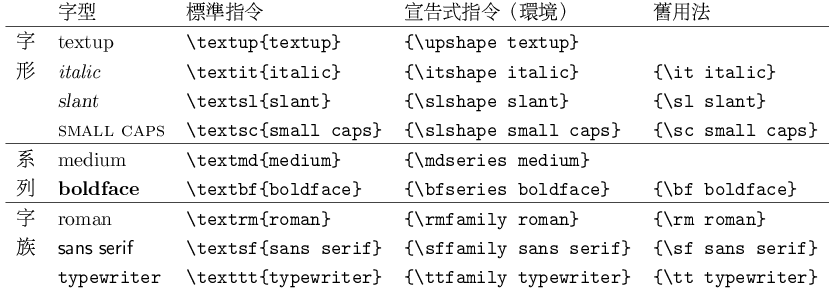
\includegraphics{fntshape}
\end{quote}
\end{htmlonly}

���O�~�F�@���A�o�O����i�`���C�䤤 upright, medium, roman ���O�@�˪��A�o�O�@�몺���`�r�A�N�����·Хh�]�w�L�F�A���D�O�n�b�S�w�r���d����Y�A���s���ܦ����`�r��C�q�e���һ���²�٪��r��A�A�M text, family, series, shape �h�t��ӨϥΡA�o�˥u�n�O�o²�ٴN��F�A�Ҧp�Gitalic ���N�O \verb|\textit{}|�C���M�]�i�H�ϥΡu���Y�B�v���¥Ϊk�A���o�]���O���򰽦Y�B�A�L�O��l Plain \TeX\index{Plain \TeX} �ҩw�q���A�b�ª��� \LaTeX\ 2.09 �]�ۮe�L�Ӫu�ΡA�å[�H�X�R�C���p�G�ϥ��¥Ϊk�A�����ɲզX�������ܮɥi��|�L�ġA�Ҧp�ʱ���o�ز���M����]�w�V�X�ɡA�N�L�k���Ͳʱ���F�A�o���٬O�o�ĨĨϥΥ��μз� \LaTeX\ �����ܪk�C

�n�`�N���O�A�j�A������m�A�ŧi�������O�A��ӧ@�νd��O�s���O�@�_�]�����A�L�i�H�������ҨӨϥΡA�Ҧp \verb|\begin{itsahpe}|, \verb|\end{itshape}|�A�o�˦b�o�����Ҥ�����r�N�q�q�|�ϥ� italic ����A�]�i�H���[�ѼƨϥΡA�Ҧp \verb|\itshape|�A�o�˥H�U����r�q�q�|�ϥ� italic ����A���ܥt�@�ӧ��ܦr�������O�X�{����C�зǫ��O���@�νd��h�O�������O���@�ӰѼơA�o�ǰѼƬO�X�{�b���O�᪺�j�A�������C�{�b�N�ӹ�ڽsĶ�ӨҤl�լݬݡG

\begin{quote}
\begin{verbatim}
% example8.tex
\documentclass{report}
\title{\bfseries Aesop Fables}
\author{Aesop\thanks{Thanks to the reader.}
       \and Nobody\thanks{Thanks to nobody}}
\date{\today}
\begin{document}
\maketitle
\tableofcontents
\chapter{Aesop Fables}
\section{The \textsl{Ant} and the \textsl{Dove}}

\itshape
An antwent to the bank of a river to quench its thirst, and
being carried away by the rush of the stream, was on the
point of drowning.
\upshape

A \textsl{Dove} sitting on a tree overhanging the water plucked a
leaf and let it fall into the stream close to her. The \textbf{\textsl{Ant}}
climbed onto it and floated in safety to the bank.

\section{The {\it Dog}\/ in the Manger}

A \textbf{\textit{dog}} lay in a manger, and by his growling and snapping
prevented the oxen from eating the hay which had been
placed for them.

``What a selfish Dog!'' said one of them to his companions;
``he cannot eat the hay himself, and yet refuses to allow
those to eat who can.''

\chapter{The \textsc{Eagle} and the Arrow}

An \textsc{eagle} sat on a lofty rock, watching the movements of a
Hare whom he sought to make his prey.

An archer, who saw the \textsc{Eagle} from a place of concealment,
took an accurate aim and wounded him mortally.
\end{document}
\end{verbatim}
\end{quote}

�ڭ̧� title page\index{title page} �����D�令����]�Ъ`�N�A�ŧi�����¥Ϊk�A�j�A���O����O�M��r��ӬA�����^�A�� Dove �令 slant ����A�� dog �令 italic �ʱ���\footnote{�Ъ`�N�A�o��ر���O���@�˪��Aslant �O�@�륿�`���r�A�u�O��L�ɱ׭Ө��צӤw�A�� italic �h�O�t�@�ؿW�S���r���]�p�C}�A�� ant �令 slant �ʱ���A�� eagle �令 small caps�C�ѩ󳹸`���D�쥻�N�|�ഫ������A�ҥH���`���D�������A����N�������Ƴ]�F�C

���o�̵o�{�Ҥl�̲ĤG�����D���� Eagle �èS�����ܦr��A�ӥB�H {\tt latex} �sĶ�ɷ|���ͥH�U�����~�]�o�ǰT���]�|�b {\tt example8.log} �����^�G

\begin{quote}
\begin{verbatim}
  ...
LaTeX Font Warning: Font shape `OT1/cmr/bx/sc' undefined
(Font)              using `OT1/cmr/bx/n' instead on input line 4.
  ...
LaTeX Font Warning: Some font shapes were not available, defaults substituted.
  ...
\end{verbatim}
\end{quote}

�{�b�ڭ̬ݨ�F�e���ҽͪ��ݩ�²�١A�o�b \LaTeX\ �N�|�ϥγo���ݩʨӪ��ܦӵo�X�T���A�o�� \verb|OT1/cmr/bx/sc| �N���ܤF OT1 �s�X�AComputer Modern Roman �r�ڡABold extended �t�C�A�ӥB�O small caps �Ϊ����r���A���~�T����ܡA�L�èS���w�q�A�]���A�o�Ӧr���N�|�ϥιw�]���r���ӥN���A�o�̴N�O�H n ���`�Ϊ��� bx �t�C�r���Ӵ��N�C�ҥH�A�r�����O�ä��O���i�H�H�N�զX���A���ǬO�ڥ��N�S���o�ئr���A���ǫh�O�S���Υ����h�w�q�n�A�o�� \LaTeX\ �N������r�F�A���O��ߡA���h�N�O�ϥιw�]���r���}�F�I

�t�@�ӫܩ_�Ǫ��a��A�N�O�Ĥ@���B�ĤG�`�����D�A������O \verb|{\it Dog}\/ in the...}|�H�o�Ӵ��J�� \verb|\/| �O����F��H�o�O \TeX\ �t�νվ����r�]�]�A iatlic �� slanted�^�M���`�r�������ťժ��@�ӫ��O�A�٬� italic correction\index{italic correction}�C�o�ˡA�b����r�M���`�r�������ťդ~�|���`�C���������L��������O�S���[�o�ӽվ�O�H�o�O�]�� \LaTeX\ �����b�]�p�ɴN���Ҽ{��o�Ӱ��D�A�ҥH \verb|\textit{}| �o���зǫ��O���|�۰ʽվ� italic correction�A�����ѧڭ̤�ʽվ�C

�t�~�A���`���D���N�|�۰��ഫ������A���D�W�� dog ������S���ܲ���H�o�b�e��������L�A�o���¥Ϊk���ɬO�L�k�ƦX�ϥΪ��A����S���骺���O�|�Τ��W�ӡC�]���A��ij�ɶq�ϥ� \LaTeX\ ���Ĥ@�ؼзǫ��O�ӧ��ܦr���C�ϥ� \verb|{\it ...}| �� \verb|{\itshape ...}|\footnote{�ŧi�����O�i�H�ƦX�ϥΡA�����M�|�ݭn��ʰ� italic correction�C} �o�ث��O���ܡA�N�o�ɮɪ`�N italic correction �����D�A�]�o�`�N�O�_�i�H�ƦX�ϥΫ��O�����D�A�ҥH�A�٬O���n���i���n�C:-)

��U�O�ƪ��X�Ӫ����G�G

\begin{quote}
\url{http://edt1023.sayya.org/tex/latex123/example8.tex} \\
\url{http://edt1023.sayya.org/tex/latex123/example8.pdf}
\end{quote}

\subsection{�۹�r���j�p���վ�}

���U�ӽͳ̫�@�Ӧr���j�p�ݩʪ��վ�A�o�b�ϥΤW�����¡A�u�n���D���O�N�i�H���W���ӨϥΡC���O \TeX/\LaTeX\ �t�Τ��A�ͨ�r���A���Y�@��a�p�A�Ҧp�e���ͨ쥿�`������r���j�p�O 10pt�A�{�b�p�G�Q�s�@�����A�ݭn 64pt ���r���ɭԴN�|�o�{�A�]���X�ӤF�I���` \LaTeX\ ���w�q�A�r�����j�p�d��O�b 5--24.88pt �����A�W�X�o�ӽd�򪺦r�ݭn��L�� package �������C\footnote{�o�O \LaTeX\ ���������w�q�����D�A�]���L�D�n�O�w��@��ʤ��ή��y�A\TeX\ ��������O�A�i�H���r����j�� 2047pt�C}

�o�̧ڭ̥��Ӭݬݤ��� 10pt �ɦU�ئr���j�p���O�B��ڨҤl�Ψ�j�p�]�o�O�۹�j�p�A�|�H����w�]�r���j�p�Ӧ۰ʽվ�^�G\footnote{�Ъ`�N�A���� pdf �榡����ϥ� 12pt �r���j�p�A�C���Ψ䤤���Ҥl�A�O�ѥt�~ 10pt �w�]�r���j�p�һs�@�� eps ���ɤޤJ�A�H�K���u�C}

\begin{quote}
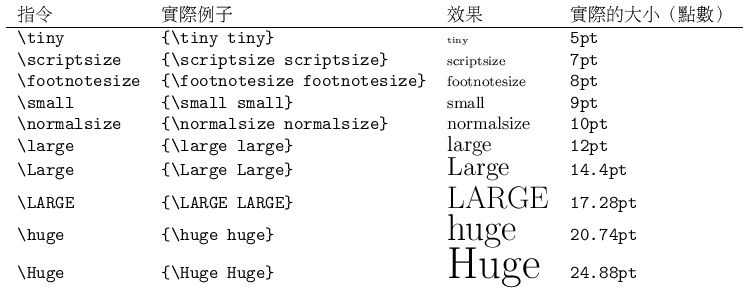
\includegraphics{fntsize}
\end{quote}

�o�Ǧr���j�p���O�]�i�H�������ҨӨϥΡA�Ҧp�G

\begin{quote}
\begin{verbatim}
\begin{small}
  ���夺�e
\end{small}
\end{verbatim}
\end{quote}

�o�˥Τ]�O�i�H���C

\subsection{����r���j�p���վ�}

�q�`�r�����j�p\index{�r��!�r���j�p}�A�ϥΤW�@�`�һ����۹�r���j�p�ӽվ�|�����K�A�ӥB����Ӫ������t�X�]�|�������A�Ҧp��Z�]�|��۰��A�����վ�A�p�G�ۦ�ε���r���j�p����k�ӽվ�r���j�p���ܡA�`�`�|�y����Z���@�P�����ΡA�]���A�p�D���n�A���ɶq�קK�C

�����ɭԴN�O�ݭn���o�˪��վ�A�Ҧp����ʭ����r���j�p�A�a�ϬO \LaTeX\ �w�]���̤j�r���]ı�o�y�p�F�I�A�o�N�n�t�~�ޤJ package �վ�F�C

�o�̧ڭ̨ϥ� \textsf{type1cm}\index{type1cm@\textsf{type1cm}} package �ӽվ�C���M�A�o�ϥ� Type 1 �r���A�~�i�H�F��L�q��j�B�Y�p���ت�%
\footnote{\LaTeX\ �t�Τ����r����j�A�b 10pt �H�W�A�O�H 1.2 �����Ƭ�����ө�j���A�]���A���� 10pt ���r���j�p���ܡA���|�� 13pt �o�ؤj�p���r���A\LaTeX\ �|��γ̬۪�j�p���r���Ӵ��N�C}%
�A�ӳo�� package �]�O�t�X Type 1 �r���ϥΪ��C�ӧO��j�� pk �I�}�r�A�o�̴N���Q�פF�A�ثe���j������ Computer Modern �r�����w�� Type 1 �� free �����A�ӥB�U�� \TeX\ distribution ���|���W�A�ϥΤW�|����K�C�H�U�O \textsf{type1cm} ���ϥΤ�k�G

\begin{quote}
\begin{verbatim}
  ...
\usepackage{type1cm}
  ...
\fontsize{�r���j�p}{��Z�j�p}\seclectfont
  ...
\end{verbatim}
\end{quote}

�ٰO�o�p��ޥΥ����M��\index{�����M��}�ܡH�аѦҲ� \ref{ch:syntax} ���B�� \ref{sec:struct} �`�A�� \ref{subsec:preamble} �p�`�������C

�䤤���u�r���j�p�v�N�O�ҭn���w���j�p�A�q�`�H pt �����A���M�A�n�ϥΨ�L���]�O�i�H�C�u��Z�j�p�v�]�O�n�@�֫��w�A���i�ٲ��C�̫᪺ \verb|\seclectfont| �O���L�o�ͧ@�Ϊ��N��A\LaTeX\ ��������r�������C�����O�A�n�U \verb|\seclectfont| ��~�|�@�ΡA\verb|\fontsize{}{}|\index{fontsize@\verb=\fontsize=} ���O�䤤���@�C

\section{���ӦC}

����O���ӦC\index{���ӦC}�H�@�� \LaTeX\ �J��˱׽u\index{�˱׽u}�|�{���O�@�ӫ��O���}�l�A�p�G�s��ӫ��O���n�L�X���ɭԩO�H�o�ɴN�n�Ψ���ӦC�����O�����ҤF�C

\subsection{���ӦC���O}

�p�G�u�O�@�p�q����r�n���ӦC�A���ϥΫ��O�|�����K�A�o�ӫ��O�N�O \verb+\verb|��r���e|+\index{verb@\verb=\verb=}�A�䤤�� \verb+|+ �o�ӲŸ��i�H�ϥΨ�L�D�r�����Ÿ��N���A�u�n�e��ۦP�N��F�A�Ҧp�G\verb|\verb+��r���e+| �o�ˤ]�O�i�H���C

\subsection{���ӦC����}

�p�G�O�@��q�����e�n���ӦC���ܡA�ϥ����ҷ|�����K�A���K�O {\tt verbatim} ���ҡC���ެO���@�ح��ӦC�����ΡA�w�]�O�ϥΥ��r���r�ڪ��r������ܪ��C���U�O�@��²�檺�Ҥl�A�������ӦC���O�����Ҫ��ϥΡG

\begin{quote}
\begin{Verbatim}[commandchars=+\[\]]
% example9.tex
\documentclass{article}
\begin{document}
The example of \verb|\verb{}| command and \texttt{verbatim} environment.

\section{\textbackslash{}\texttt{verb} command}

When you want to express you home directory, you can \verb|echo $HOME|
varient to display your home directory in your sh script.

\noindent
\verb*|This is    4 space here.|

\section{\texttt{verbatim} environment}

Here is a sh script to determine if on GNU/Linux system.

\begin{verbatim}
#!/bin/sh
Date=`date '+%y%m%d'`
if [ `uname` = Linux ]
then
  Mail=/var/spool/mail/edt1023
  Target=/mnt/hd
else
  Mail=/var/mail/edt1023
  Target=/mnt/pub
fi
\end{verbatim}
\end{document}
\end{Verbatim}
\end{quote}

�o�̷|�o�{�@�ǩ_�Dz{�H�A�Ҧp
\texttt{\textbackslash{}verb*}
���ӬP���O����N��O�H�N�O���ťեH
%begin{latexonly}
\verb*| |
%end{latexonly}
\begin{htmlonly}

\includegraphics{blank}
\end{htmlonly}
���覡���ܥX�Ӫ��N��A{\tt verbatim} ���Ҥ]�O�i�H�o�˨ϥΡC�Ҧp {\tt example9} �����G

\begin{quote}
\begin{verbatim}
\verb*|This is    4 space here.|
\end{verbatim}
\end{quote}

�]�i�H�g���G

\begin{quote}
\begin{Verbatim}[commandchars=+\[\]]
\begin{verbatim*}
This is    4 space here.
\end{verbatim*}
\end{Verbatim}
\end{quote}

�t�O�b��A���Ҫ��W�U��|�h�ťX�Ӫťզ�X�ӡC

�t�~�A���D�����򤣨ϥ� \verb+\verb|\verb|+ �N�n�F�O�H��]�O���ӦC�����O�M���ҳ����������L���O���ѼơA���D�����N�O�@�ӫ��O�A�ҥH \verb+\verb+ ����b���Y�C

�ϥ� \verb|\textbackslash|\index{textbackslash@\verb=\textbackslash=} �o������ԭz�A�Ӥ��� \verb|$\backslash$| �o��²�檺�覡�A��]�O�o�Ӥ�Z���ϥ� \LaTeX{}2{\tt HTML} ���ন HTML �榡�A�ϥ� \LaTeX\ �����N���ܪk�|�ন�@�몺�Ÿ��A���ϥΫ�̪��覡�h�|�ন���ɡA�ҥH�o�̴N�ϥ� \LaTeX\ �����N���ܪk�F�C

���U�O�ƪ��X�Ӫ����G�G

\begin{quote}
\url{http://edt1023.sayya.org/tex/latex123/example9.tex}\\
\url{http://edt1023.sayya.org/tex/latex123/example9.pdf}
\end{quote}

\section{�[�J����}

�o�̥u�����p��ϥ� \textsf{CJK}\index{CJK@\textsf{CJK}} package �����ΡA��]�O�@�� \TeX\ distribution �|���W�]���ǵo��M��èS�����W�A�o�ɥu�n�ۦ�w�ˤF�^�C\textsf{CJK} package �O�⤤�媺�����]�b�@�����Ҹ��Y�A�b�o�����Ҥ��N�i�H�ϥΤ���A���}�o�����ҴN�S�^�_��쥻���^�����ҡA���U�ѨҤl�ӻ����C

\begin{quote}
\begin{verbatim}
\documentclass{article}
\usepackage{CJK}  % �ϥ� CJK �����M��
\begin{document}
% �i�J CJK ���ҡA�èϥ� Big-5 �X�� hwmm �o�Ӧr��
\begin{CJK}{Bg5}{hwmm}
\section{CJK �����M��}
�o�O�@�Ӵ��աA���� CJK package �����աC
\section{��᷽�O�`��}
��U�A�׳q�H�F�_��ƤQ�B�A�ŵM�}�ԡC�g�a���m�A�Ϊ��k�M�C���}�СB�����B%
��B�ˤ��ݡA�魯��q�A�����ۻD�C�䤤���Ӻا@�A�k�k��ۡA�x�p�~�H�F���v�B%
���ԡA �éɵM�ۼ֡C�����H�A�D�j��A�ݩұq�ӡF�㵪���A�K�n�ٮa�A�]�s�B�����B%
�@���C�����D�����H�A�w�ӰݰT�C�ۤ��G�u���@�ׯ��ɶáA�v�d�l���H�Ӧ����ҡA%
���_�X�j�F�E�P�~�H���j�C�v�ݤ��O��@�F�D�������~�A�L���Q�B�ʡC���H�@�@%
���㨥�һD�A�Ҽ۱{�C�l�H�U�_���ܨ�a�A�ҥX�s���C���Ƥ�A��h�C�����H�y%
���G�u�������~�H�D�]�C�v
\end{CJK}
\end{document}
\end{verbatim}
\end{quote}

�N�o��²��C�u�O�sĶ�n��� {\tt bg5latex}\index{bg5latex@\texttt{bg5latex}} �Ӥ��O��Ӫ� {\tt latex} ���O�A�o�O���F�׶}�ڭ� Big-5 �X���@�ǯS���X�����Y�A�ٰO�o����C��̫�n�[�Ӧʤ��� \verb|%|\index{%@\verb=%=} �ܡH�o�ˤ~���|���J�^�媺�r���ťաC�sĶ�n���Ҥl�p�U�G

\begin{quote}
\url{http://edt1023.sayya.org/tex/latex123/example10.tex}\\
\url{http://edt1023.sayya.org/tex/latex123/example10.pdf}
\end{quote}

�ԲӪ� \textsf{CJK} package ���ϥΤ��廡���A�аѦ� \textsf{CJK} package �Ҫ������Ρq�ڪ� CJK�r�@��G

\begin{quote}
\url{http://edt1023.sayya.org/tex/mycjk/mycjk.html}\\
\url{http://edt1023.sayya.org/tex/mycjk/mycjk.pdf}
\end{quote}


% ``�j�a�Ӿ� LaTeX'' LaTeX ��Z space.tex
% Copyright (c) 2004  Edward G.J. Lee <edt1023@info.sayya.org>
%
% �b���H�� GNU Free Documentation License 1.2 �ΥH�᪺�����W�d���U�A
% ���\�����B���G�έק�C���쪩�v�B���v�n�����o�����C
%
% �����G�����A�t�� fdl.tex�A���e�� GNU FDL ���W�d���C�p�G�򥢡A�i��
% http://www.gnu.org ���o�A�μg�H�ܦۥѳn�����|(Free Software Fundation)
% �����C
% 9 Temple Place - Suite 330, Boston, MA 02111-1307, USA.
%
% $Id: space.tex,v 1.23 2004/03/07 12:20:47 edt1023 Exp $
%
\chapter{�Ŷ��P��m}
\label{ch:space}

�e�@��������L�A�Ƿ|����Ŷ��N�Ƿ|�ƪ��F�IKnuth\index{Knuth} �б¦b�L�� \textit{The \TeX{}book}\index{The TeXbook@\textit{The \TeX{}book}} �@�Ѥ��]���ήe�ϥ� \TeX\ �ƪ������ΡG�@�Ӫ����N���@�ӧt�������]glue\index{glue}�^�������A�M��C�@�ӭn�ƪ������e�N�O�U�ؤ��P�� box\index{box}�A�b�o�� box �٨S���T�w���T��m�ɡA���O�i�H���ʪ��]�����٨S�����^�A�@���ƪ������A�����N���F�A��O�C�� box ����m�N�T�w�L�k�A���ʤF�A���D�S�q�Y�A�ӡC

�@�Ӧr���B�@�ӳ�r�B�@�ӥy�l�B�@�Ӭq���B�@�ӲŸ��B�@�ӹϧΡB�@�Ӫ��泣�i��c���@�� \TeX\ �� box�A�Ʀ� box ���٦� box �����ΡC�o���Q�Q�ת��A�N�O�o�� box �p��w�m�L�̨쥿�T����m�A���C�� box �������Ŷ�����F����n�B�A�ҥH�A�쩳�O�b���� boxes ���ݩʡB��m�A�٬O�վ� glue ���Ŷ��A�N�ݦU����h�ݫݤF�]�Ъ`�N�Abox ���@�w�O�i�����I�b \TeX\ ���Y�Aglue �O�i�H�վ㪺�C�^�C

�ڭ̫e���ҰQ�ר쪺�^��y�I��ťժ��վ�Bitalic correction\index{italic correction}�B\verb|\linespread|\index{linespread@\verb=\linespread=} �� \verb|\parindent|\index{parindent@\verb=parindent=} �o�dz��O�b�վ� glue�C�q�`�A�b \LaTeX\ �t�θ��Y�A���w���`�`���|�O����T�w���A�|�����ΰ��p���ת��۰ʷL�աA�o�O�����Ŷ��t�m�W���ݭn�C

\section{\LaTeX\ ���ϥΪ��׶q���}
\label{sec:units}

�n��T�y�z�M�վ� \LaTeX\ �����Ŷ��Φ�m�A�ڭ̥��ݭn���ӼзǪ��׶q���C�H�U���O�b \LaTeX\ �`�|�Ψ쪺���C�o�̦�������ά۹��줧���A���D���n�A���M�A�@��O��ij�ϥά۹���A��]�O�A�L�|�H�ۤ�Z�r���j�p���ܮɸ�۰��A�����վ�C���M�A�b�����D��T�B�T�w�j�p����ܮɡA�N�o�ϥε�����F�C

�o�̦p�G�O�\�� HTML �榡�����A�Хt�Ѧ� PDF �榡�����A�H�K���ܤW���u�C�H�U���椤�ҵe�X�Ӫ����׶ȨѰѦҥΡC

\subsection{������}
\index{������}

%begin{latexonly}
\begin{quote}
\begin{tabular}{>{\tt}lll}
���W�� & �N�q & ���� \\
\hline
pt & point, $1/72.27$~inch & \drawwidth{1pt} \\
bp & Adobe big point, $1/72$~inch & \drawwidth{1bp} \\
pc & pica, 12pt & \drawwidth{1pc} \\
mm & millimeter, $1/25.4$~inch & \drawwidth{1mm} \\
cm & centimeter, 10mm & \drawwidth{1cm} \\
in & inch, 25.4mm & \drawwidth{1in} \\
\end{tabular}
\end{quote}
%end{latexonly}

\begin{htmlonly}
\begin{quote}
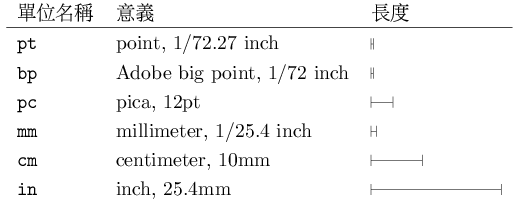
\includegraphics{a-units}
\end{quote}
\end{htmlonly}

�o�̭n�`�N���O \TeX/\LaTeX\ �t�Τ��ҿת��I�]point�^\index{�I�]point�^}�A�����O�@�몺 printer point\index{printer point}�A�]�N�O $1/72.27$~inch�A���b Adobe ���W�椤�A�Ҧp \textsc{PostScript}\index{PostScript@\textsc{PostScript}} �y�������ҿ��I�A�L�O big point\index{big point}�A���� $1/72$~inch�]�p���I�������˥h�F�^�A�|��@�몺 print point �y�L�j�@�I�I�C

\subsection{�۹���}
\index{�۹���}
%begin{latexonly}
\begin{quote}
\begin{tabular}{>{\tt}lll}
���W�� & �N�q & ���� \\
\hline
em & �����b�ϥΦr���r�� M ���e�� & \drawwidth{1em} \\
ex & �����b�ϥΦr���r�� x ������ & \drawwidth{1ex} \\
\end{tabular}
\end{quote}
%end{latexonly}

\begin{htmlonly}
\begin{quote}
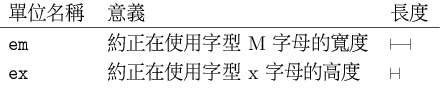
\includegraphics{r-units}
\end{quote}
\end{htmlonly}

�b \TeX\ ���Y�ҿת� em\index{em}�A���A��T�Ө��O���b Knuth �б³]�p�� Computer Modern �r�����Y�� em-dash\index{em-dash} ���e�סA�ѩ�r�� M ��ڤW�O�]�b�r���W�ҿת� em-square ���Q��椤�A�� em �ҫ����e�׬O���o�� em-square\index{em-square} ���e�סA���r�� M �����ä��������o�� em-square�A�]���o�˴N�|�y���t���F�C�ҥH�H�r�� M ���e�רӻ������ܮe�����øq�C\LaTeX\ ���ӫ��O \verb|\quad|\index{quad@\verb=\quad=} �o�N�O���ͤ@�ӥ��T em ���e�ת��ťաA�ҥH�b Knuth �бª� \textit{The \TeX{}book} ���A���� em �N�������L�O�@�� `quad' ���e�סC


\section{�����j�p}
\label{sec:layout}\index{�����j�p}

�ڭ̹��ү౱��@��i�Ȫ��d�򳣥i�H�٬������C���M�A�ڭ̪�����]body�^\index{����]body�^}�ä��O������i�Ȫ��d��A�W�U���k���|�d���@�w���ťաC�p�ɭԦb�ůȤW�m�߼g�򵧡A�Ѥ@�������|�n�ڭ̯d�u�Ѧa�v�A�o�N�O������|�P���ťաA���F��ı�W���z�ѡA�j���]�O�H�ͪ����z�a�H:-)

�b�s��W�A�]���H�٤���]body�^���������u���ߡv�Ρu���f�v\index{����}\index{���f}�A�|�P���ťճ����A�h�٬��u����v\index{����}�C��}���ߡB���䪺�]�p�A�N�٤����u�X��v\index{�X��}�A�Ҧp�A�H�I���ϧG����i�ȷ����O�I�������X�A�H�o�ӭI���ϦӨ��A�N�L�ҿת���F�C���o�b \LaTeX\ �q�`�O���|���o�ر��p�X�{�A���D�S�N�h���w����M�ȱi�j�p�P�˽d��C

���M�A�b����H�~���ťաA�]�ëD���O�ťաA�L�]�t�F�����]footer�^\index{�����]footer�^}�A���ܡ]header�^\index{���ܡ]header�^}������]marginal note�^\index{���}\index{marginal note}�������A�O�����󭶼ơB���ѵ���T�C

\subsection{�����ϸ�}
\label{subsec:layout}

\begin{quote}
\begin{center}
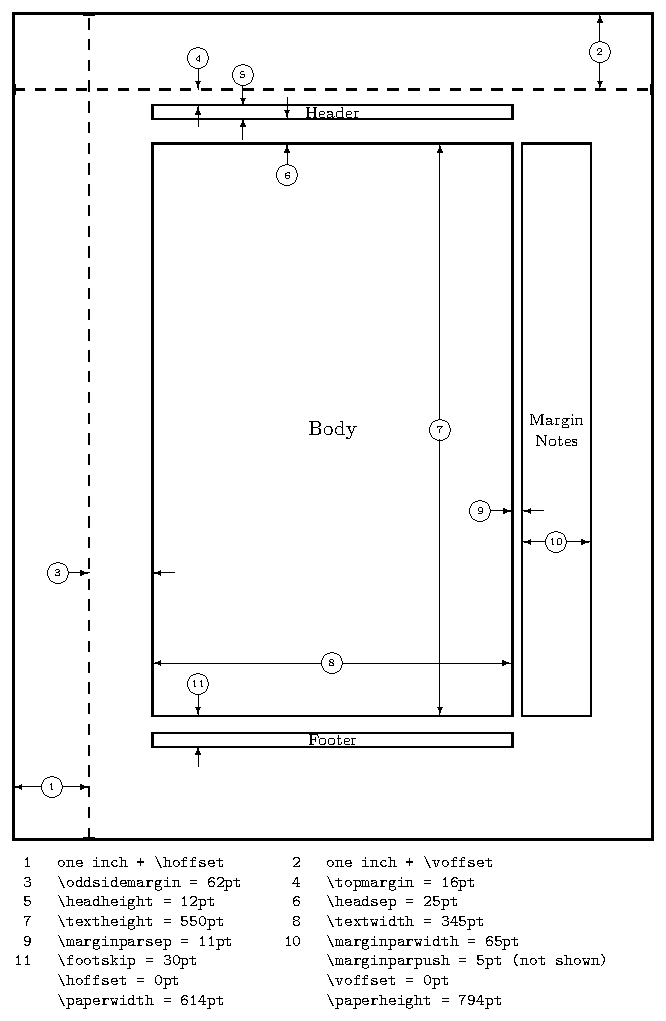
\includegraphics{layout-r}
\end{center}
\end{quote}

�o�̩ҿת��ȱi�j�p\index{�ȱi�j�p}�A�����O {\tt paperwidth}\index{paperwidth} �M {\tt paperheight}\index{paperheight} �ҳ򦨪��d��A�ëD��ڤW��W���쪺�ȱi�j�p�A��ڦb��W���ȱi�q�`�|���j��ڭ̳o�̪��ҿׯȱi�A�ҥH�A�����C�L�ɡA�ٻݰ��L�թκI���~�|�O�u�����o�̩ҿת��ȱi�j�p�]�����j�p\index{�����j�p}�^�C

�o�O 10pt ����j�p�A�p�G�����w�ȱi���ܡA\LaTeX\ �w�]�|�ϥά��� {\tt letterpaper}\index{letterpaper} ���j�p�A�p�n�ϥμڡB�馡�� {\tt a4paper}\index{a4paper} ���ܡA�n�t����w�C�ڭ̥i�H�y�L�ݤ@�U \LaTeX\ �w�]�O�p��w�ƪ����Ŷ����C�䤤 Header�]���ܡ^�BFooter�]�����^��������Ŷ��O���t�A�b���� Body ���Y���A�o�̬O�u�O�歱���ϡA�p�G�O�������ܡA�����ƭ��M�_�ƭ�������O�n���k�ﴫ���A�]�N�O���o�ӹϬO�_�ƭ��A���ƭ����ܡA����O�b����C

�o�̧ڭ̨Ӭݤ@�U�o�ǭȩҥN�����N�q�G

\begin{quote}
\begin{tabular}{ll}
���O�]�ȡ^& �N�q \\
\hline
\verb=\paperwidth=	& �ȱi���e�� \\
\verb=\paperheight=	& �ȱi������ \\
\verb=\textwidth=	& ����]body�^���e�� \\
\verb=\textheight=	& ����]body�^������ \\
\verb=\headheight=	& ���ܡ]header�^���� \\
\verb=\headsep=		& ���ܻP���嶡���Z�� \\
\verb=\footskip=	& ���婳�ܭ��������Z�� \\
\verb=\topmargin=	& ���ܤW�誺�ť� \\
\verb=\marginparwidth=	& ������e�� \\
\verb=\marginparsep=	& ����P���媺�Z�� \\
\verb=\marginparpush=	& ��������Z \\
\verb=\oddsidemargin=	& ���奪�䪺�ťդj�p \\
\verb=\hoffset=		& �L�ժ����b��گȱi�����k��m \\
\verb=\voffset=		& �L�ժ����b��گȱi���W�U��m \\
\index{paperwidth@\verb=\paperwidth=}\index{paperheight@\verb=\paperheight=}%
\index{textwidth@\verb=\textwidth=}\index{textheight@\verb=\textheight=}%
\index{headheight@\verb=\headheight=}\index{headsep@\verb=\headsep=}%
\index{footskip@\verb=\footskip=}\index{topmargin@\verb=\topmargin=}%
\index{marginparwidth@\verb=\marginparwidth=}\index{marginparsep@\verb=\marginparsep=}%
\index{marginparpush@\verb=\marginparpush=}%
\index{oddsidemargin@\verb=\oddsidemargin=}%
\index{hoffset@\verb=\hoffset=}\index{voffset@\verb=\voffset=}%
\end{tabular}
\end{quote}

\verb|\hoffset| �� \verb|\voffset| �N�O�b�վ㪩���b��گȱi�W�����T��m�A�o�˦L�X�Ӫ��ɭԤ~�|�b��گȱi�������C

�Y���F�ܡH�o�ܥ��`�A�]�� \LaTeX\ �������]�w��챵IJ���H�ӻ��A�O�c�W�L�����x���B�·СA�]���o�̤��h�ͥL���]�w�A��}�l��b�S�����n��ɶ���b�o�Ӧa��C�p�G��ڷQ�վ㪩���A��ij�ϥ� {\sf geometry}\index{geometry@\textsf{geometry}} package�C�|�ӨҤl�A�Q���U��t�O 2cm �N�n�A���u�n�b preamble\index{preamble} �ϳ]�w�G

\begin{quote}
\begin{verbatim}
\usepackage[margin=2cm]{geometry}
\end{verbatim}
\end{quote}

�N�i�H�F�A�p�G�H 12pt �j�p���r�A{\tt a4paper} �ȱi�j�p���]�w���ܡA�H����Ө��A�j���O�C�� 40 �Ӥ���r�A�o�O���媺�e�סC�i�H�����Φۦ�վ� {\tt margin}\index{margin} ���ȴN��F�C�ڭ̫ܧƱ�A�U�@���� \LaTeX\ ���o�譱���ﵽ�A�H��K�ϥΪ̳]�w�C
%���T�B�ԲӪ��]�w��k�A�ڭ̯d��᭱�������y���ѮɦA�ӽ͡A�o�˴N���P�v�T�ڭ̾Dzߪ����`�i�סC

\subsection{�ȱi�j�p}

\begin{quote}
\begin{tabular}{>{\tt}ll>{\tt }ll}
�ȱi & �j�p & �ȱi & �j�p\\
\hline
a4paper        & 21x29.7cm & letterpaper    & 8.5x11in \\
a5paper        & 14.8x21cm & legalpaper     & 8.5x14in \\
b5paper        & 17.6x25cm & executivepaper & 7.25x10.5in \\
\end{tabular}
\end{quote}

�ܩ�p����w�ȱi�j�p�A�o�̥�²�满���@�U�o�g�峹���]�w�A�ͨ� \LaTeX\ ����Z���O�ɷ|�A�Բӻ����C

\begin{quote}
\begin{verbatim}
% ���媺�]���O�]�w
\documentclass[12pt,a4paper]{report}
\end{verbatim}
\end{quote}

�ҥH�A�o�g�峹�ϥΪ��O {\tt a4paper}�A����r�����j�p�O 12pt�C��A�����ѼƬO�ﶵ�A�i�H�ٲ��A�p�G�ٲ����ܡA�w�]�ȴN�O 10pt/{\tt letterpaper}�C

\section{�վ��V�Ŷ�}

�o�̪���V�Ŷ��A�Ҧp \verb|~|\index{~@\verb=~=} �o��r�����`�ťաA�� \verb|\quad| �o�� em\index{em} �e�תťաA���O�b�վ��V���ťաC���p�G�O�n��j�B�Χ�p���ťծɸӦp��վ�O�H���U�ڭ̴N�Ӭݬ� \LaTeX\ �������򱱨���O�i�H�B�ΡG

\subsection{�վ��V�Ŷ������O}

\begin{quote}
\begin{tabular}{ll}
���O & �N�q \\
\hline
\verb=\hspace{���}= & �V�k�ťX�Y�ӫ׶q��쪺�ťաA�p�G�O�t�ơA�h�O�V�� \\
\verb=\hfill=        & �����k��Ǫ���r�������X�i�ܤ@�Ӧ�e���� \\
\verb=\quad=         & �ťX�@�� em ��쪺�ť� \\
\verb=\qquad=        & �ťX�G�� em ��쪺�ť� \\
\verb=\thinspace=    & �ťX $1/12$ �� em ��쪺�ť� \\
\verb=\enspace=      & �ťX $1/2$ �� em ��쪺�ť� \\
\verb=\dotfill=      & �@�ΩM \verb|\hfill| �ۦP�A�u�O�ť��ܦ��I \\
\verb=\hrulefill=    & �@�ΩM \verb|\hfill| �ۦP�A�u�O�ť��ܦ��@��u \\
\verb=\centering=    & �����O�H�᪺��r�N�|�~���ƦC�A���k�u�N������ \\
\verb=\raggedright=  & �����O�H�᪺��r�N�|�~���ƦC�A�k�u�N������ \\
\verb=\raggedleft=   & �����O�H�᪺��r�N�|�~�k�ƦC�A���u�N������ \\
\verb=\centerline{}= & �N�j�A��������r�~���ƦC
\end{tabular}
\end{quote}
\index{hspace@\verb=\hspace=}\index{hfill@\verb=\hfill=}%
\index{quad@\verb=\quad=}\index{qquad@\verb=\qquad=}%
\index{thinspace@\verb=\thinspace=}\index{enspace@\verb=\enspace=}%
\index{dotfill@\verb=\dotfill=}\index{hrulefill@\verb=\hrulefill=}%
\index{centering@\verb=\centering=}\index{raggedright@\verb=\raggedright=}%
\index{raggedleft@\verb=\raggedleft=}\index{centerline@\verb=\centerline{}=}

�@�檺�歺�ϥ� \verb|\hspace{���}| �ɱN�|���ġA�o�ɥi�H�[�ӬP���A�Ҧp \verb|\hspace*{3em}|�C

�b�ϥ� \verb|\centerline{}| �����X�A���u��y�ܤ�K�A�]���L���|�v�T�H�U����r�A���L�]���|���A�Ʀܥ[�J����Ÿ��]�L�ġC�ҥH�p�G��y���׶W�L�@�檺��e�A�L�|�W�X��ɡA�ƦܴN��������r�N�ݤ���F�C

�䤤 \verb|\thinspace| �S�i�H�ϥ�²�ƪ� \verb|\,| �ӥN���A�D�n�O�Φb�޸����S���޸������ΡA�q�`�o�ر��ΡA��޸������n���Ӷ��j�A�H�K�Ϥ��A�Ҧp�G

\begin{quote}
\begin{verbatim}
``\,`Superman', he said.''
\end{verbatim}
\end{quote}

���{�X�ӷ|�O�G

%begin{latexonly}
``\,`Superman', he said.''
%end{latexonly}

\begin{htmlonly}
\begin{quote}
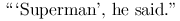
\includegraphics{superman}
\end{quote}
\end{htmlonly}

�o�ˤ~��Ϥ��X���P�޸��A�_�h�|�ܦ��@�ӳs�T�� grave accent\index{grave accent} ���޸��C�Ъ`�N�A�ѩ�o�ӫ��O�O�ѫD�r���Ÿ��c���A�ҥH�A�L���@�νd��b�J��Ÿ�������N�����F�A�᭱�����ťթΥH�j�A���ӭ����@�νd��A�N�n��������L�� \verb|\@| �@�˪����ΡC

\subsection{�վ��V�Ŷ�������}

\begin{quote}
\begin{tabular}{ll}
\verb|\begin{center}...\end{center}| & ���o�����Ҥ������e�m�� \\
\verb|\begin{flushleft}...\end{flushleft}| & ���o�����Ҥ������e�a�� \\
\verb|\begin{flushright}...\end{flushright}| & ���o�����Ҥ������e�a�k \\
\verb|\begin{raggedright}...\end{raggedright}| & ���o�����Ҥ������e�a���A�k�u�N������ \\
\verb|\begin{raggedleft}...\end{raggedleft}| & ���o�����Ҥ������e�a�k�A���u�N������ \\
\end{tabular}
\end{quote}
\index{center@\texttt{center}}\index{flushleft@\texttt{flushleft}}%
\index{flushright@\texttt{flushright}}\index{raggedright@\texttt{raggedright}}%
\index{raggedleft@\texttt{raggedleft}}

�i�J���ҡA�M�W�@�`���쪺���O�A��̦����򤣦P�O�H�̤j�����P�O�A�o�i�H��K�����w�@�ӽd�򪺤�y���L�@�ΡA�Ӥ��|�v�T���ҥH�~����y�C�䦸�A�i�J���ҡA�a�ϩM�W�U��s�b�@�_�A�S���ťX�ťզ�A�L�]�|�۰ʪ��b�W�B�U��ťX�Ӫťզ�X�ӡA�ϥΫ��O���ܫh���|�C

�x�I�o�̫��S���� {\tt raggedright} �� {\tt raggedleft}�H��ӥL�]�O�i�H�����ҨӨϥΡC�ѩ�o��ӫ��O�|�ϥH�U�����e�����B�k�u�������A�]���ϥΤW�n�D�`�p�ߡA���D���ӴN�Q�����媺���B�k�u�������A�_�h�A�̦n�O�ϥΦ��d�򭭨�覡�C���M�A�p�G�o��ӫ��O�O�Φb�Y�Ө�L���ҽd�򤺡A�L���@�Τ]�N�ȭ���o�����Ҥ��A���|�v�T�o�����ҥ~����y�C

\subsection{�ޤ�����}
\index{�ޤ�����}

�ޤ�q�`�N�O�ޥΥL�H����y�A�b�ޤ媺�q���A��dz��|�X�{���Y�����ΡA�H�K�M����۰Ϲj�A�o�]�O�@�تŶ����t�m�A�i�W�[�峹����Ū�ʡC�b \LaTeX\ ���Y���T�ؤޤ����ҡG{\tt quote}, {\tt quotation}, {\tt verse}�C�o�T�̬ݰ_�ӫܹ��A�����ǷL���t���C

\begin{quote}
\begin{tabular}{>{\tt }lll}
���� & �A�ήɾ� & �S�� \\
\hline
quote & ���u���u�ޤ� & �C�Ӭq���Ĥ@�椣���Y \\
quotation & �h�Ӭq�������ޤ� & �C�Ӭq���Ĥ@��|���Y \\
verse & �ֺq�B���ޤ� & �C�Ӭq�����Ĥ@�椣���Y�A���ĤG��_�|���Y \\
\end{tabular}
\end{quote}
\index{quote@\texttt{quote}}\index{quotation@\texttt{quotation}}%
\index{verse@\texttt{verse}}

�b {\tt verse} �����ΡA�q�`�|�ϥ� \verb=\\=\index{\\@\verb=\\=} �Ӵ���H�K����C�@�檺�e�סC�ӥB�q�����Z\index{�q�����Z}�N�����~�b�]�w���v�T�A�䤤 {\tt quote} �M {\tt verse} ���ҷ|�w���J�A�����q�����Z�A�� {\tt quotation} ���ҫh���|�C

���U�ڭ̨Ӭݬݽվ��V�Ŷ����@�Ӻ�X��ҡG

\begin{quote}
\begin{verbatim}
% example11.tex
\documentclass{article}
\usepackage{CJK}
\begin{document}
\begin{CJK}{Bg5}{hwmm}
\section{hspace}
\hspace*{2em}�o�O�@�Ӿ�V�Ŷ��վ㪺���աC\\
�o�O�@��\hspace{2em}��V�Ŷ��վ㪺���աC\\
�o�O�@�� \hspace{2em} ��V�Ŷ��վ㪺���աC
\section{hfill}
�o�O�@��\hfill{}��V�Ŷ��վ㪺���աC
\section{quad}
�o�O�@��\quad{}��V�Ŷ��վ㪺���աC\\
�o�O�@�� \quad{} ��V�Ŷ��վ㪺���աC\\
�o�O�@��\qquad{}��V�Ŷ��վ㪺���աC
\section{dotfill}
�o�O�@��\dotfill{}��V�Ŷ��վ㪺���աC\\
�o�O�@�� \dotfill{} ��V�Ŷ��վ㪺���աC
\section{hrulefill}
�o�O�@��\hrulefill{}��V�Ŷ��վ㪺���աC
\section{center}
\begin{center}
�o�O�@�Ӿ�V�Ŷ��վ㪺���աC
\end{center}
\section{flushleft}
\begin{flushleft}
�o�O�@�Ӿ�V�Ŷ��վ㪺���աC
\end{flushleft}
\section{flushright}
\begin{flushright}
�o�O�@�Ӿ�V�Ŷ��վ㪺���աC
\end{flushright}
\section{quote}
�o�O�`���ۥ���J�����`���G�ơG
\begin{quote}
An antwent to the bank of a river to quench its thirst, and
being carried away by the rush of the stream, was on the
point of drowning.

A Dove sitting on a tree overhanging the water plucked a
leaf and let it fall into the stream close to her. The Ant
climbed onto it and floated in safety to the bank.
\end{quote}
\section{quotation}
�o�O�`���ۥ���J�����`���G�ơG
\begin{quotation}
An antwent to the bank of a river to quench its thirst, and
being carried away by the rush of the stream, was on the
point of drowning.

A Dove sitting on a tree overhanging the water plucked a
leaf and let it fall into the stream close to her. The Ant
climbed onto it and floated in safety to the bank.
\end{quotation}
\section{verse}
�o�O�`���ۥ���J�����`���G�ơA�o�O�`���ۥ���J�����`���G�ơA%
�o�O�`���ۥ���J�����`���G�ơA�o�O�`���ۥ���J�����`���G�ơG
\begin{verse}
An antwent to the bank of a river to quench its thirst, and
being carried away by the rush of the stream, was on the
point of drowning.

A Dove sitting on a tree overhanging the water plucked a
leaf and let it fall into the stream close to her. The Ant
climbed onto it and floated in safety to the bank.
\end{verse}
\section{centering}
\centering
�o�O�@�Ӿ�V�Ŷ��վ㪺���աC\\ % �o�̭n����A�_�h�|�O \raggedright ���@��
\raggedright
\section{centerline}
\centerline{�o�O�@�Ӿ�V�Ŷ��վ㪺���աC}
\section{raggedright}
\raggedright
�o�O�@�Ӿ�V�Ŷ��վ㪺���աC
\section{raggedleft}
\raggedleft
�o�O�@�Ӿ�V�Ŷ��վ㪺���աC
\end{CJK}
\end{document}
\end{verbatim}
\end{quote}

�sĶ�n�����G�p�U�G

\begin{quote}
\url{http://edt1023.sayya.org/tex/latex123/example11.tex}\\
\url{http://edt1023.sayya.org/tex/latex123/example11.pdf}
\end{quote}

�n�`�N�O���O�e�᪺�ťաA�� \verb|\hspace|, \verb|\dotfill|, \verb|\hrulell| �o�����O�A���O�e��ťճ��|��i�h���C\verb|\quad|, \verb|\qquad| �o�����O�A�h�᭱���ťդ]�O�|��J���C�t�~�A�ѨҤl���i�H�ݥX�ӡA�@�� em\index{em} ���e�סA�j���O�@�Ӥ���r���e�סA�ҥH�A�ڭ̹w�]�ϥ� 10pt ���r�A�o�� em �e�״N�۷��� 10pt ���e�סA�ҥH�A�ڭ̦b�Ĥ@�洡�J�F 2em �e�ת��ťաA�]�N�n���O���Y�F��Ӥ���r�@�ˡC

\section{�վ��a�V�Ŷ�}

\begin{quote}
\begin{tabular}{ll}
\verb=\vspace{���}= & �V�U�ťX�Y�ӳ�쪺�ťա]��^�A�t�ƫh�O�V�W \\
\verb=\bigskip=     & ���� 12pt�]11--12pt�^�������ťա]��^ \\
\verb=\medskip=     & ���� 6pt�]5--7pt�^�������ťա]��^\\
\verb=\smallskip=   & ���� 3pt�]2--4pt�^�������ťա]��^\\
\verb=\vfill=       & �M \verb|\hfill| �����A�@�άO�N�Y�q���V�W���A�Ω��U�� \\
\verb=\parskip=���= & �վ����C�Ӭq�������Z�����Y�ӳ��
\index{vspace@\verb=\vspace=}\index{bigskip@\verb=\bigskip=}%
\index{medskip@\verb=\smallskip=}\index{vfill@\verb=\vfill=}%
\index{parskip@\verb=\parskip=}
\end{tabular}
\end{quote}

�䤤�� \verb|\bigskip, \medskip, \smallskip| �ëD�T�w���A�L�̷|���W�U��ߵ����ݭn�۰ʰ��L�աA�H�F��@�㭶���@�P���Ŷ��t�m�C\verb|\vspace| �p�G�O�X�{�b�@�����Ĥ@��γ̫�@��ɡA�N�|���h�@�ΡA�o�ɥi�H�[�ӬP���A\verb=\vspace*{���}=\index{vspace@\verb=\vspace*=}�C

���F�����������@�P��\index{�����@�P��}�A�ϥ��a�V�Ŷ��վ㪺���O�ɭn�S�O�d�N�A�Ҧp���`���D�W�U���Ŷ��B�U�q�������Ŷ��A�i�J���ҫe��ҪťX���Ŷ��A�o�����@�өT�w�ȡA\LaTeX\ �|�۰ʥh�վ�A�����ѨϥΪ̦ۦ�ʤ�A���D�O�ʭ��o�س�W���C�ҥH�A�ϥ��a�V�Ŷ��վ���O�ɡA�n�D�`�`�N���骺�@�P�ʡA�o�]�O�ƪ��W���@�ӫܭ��n����h�C

�o���|�o�g�峹�������ʭ�\index{�����ʭ�}���ҨӺ�X�����A��B�a�V�Ŷ����B�ΡC�ٰO�o�� \ref{sec:titlepage} �`�� title page\index{title page} �����O�ܡH���ڭ̤]�i�H�ۦ�]�p�@�ӿW�ߪ������ʭ��A�ϥΪ��O \LaTeX\ ������ {\tt titlepage}\index{titlepage@\texttt{titlepage}} ���ҡC�o�̪����ɤޥάO�ڭ��٨S���Dzߨ쪺�A�S���Y�A�u�n�j��h����N��F�C

\begin{quote}
\begin{verbatim}
% example12.tex
\documentclass[12pt,a4paper]{report}
\usepackage{CJK}     % �ޤJ�һݭn�� packages
\usepackage{graphicx}
\begin{document}
\begin{CJK}{Bg5}{hwmm}
\begin{titlepage}    % �ϥ� titlepage ����
\vspace*{5ex}
  \begin{flushright} % �j���D�a�k
    \Huge\textbf{�j�a�Ӿ� \LaTeX}
  \end{flushright}
  \rule{\textwidth}{.256ex}
  \begin{flushleft}  % �������X����a���A�M�j���D�����H�@��u�j�}
    Version 0.1 draft\\
    \today
  \end{flushleft}    % ���ɦ�󤤥�����
  \vspace{8ex}       % �ťX 8ex �������Ŷ�
  \hspace{2em}\includegraphics[scale=.75]{cover2.1} % �ޤJ���ɡA�ñN�o��
  \vspace{8ex}                                      % ���ɾ�V�k�� 2em
  \begin{flushright} % �@�̸�T�a�k
    By Edward G.J. Lee ���G��\\
    Email�G\texttt{edt1023@info.sayya.org}
  \end{flushright}
\end{titlepage}
\end{CJK}
\end{document}
\end{verbatim}
\end{quote}

�ѩ�t�X���������D�A�䤤���@�Ǽƾڦ���ʡA�ӥB�]�ٲ��F�@�ǧڭ��٨S���Dzߨ쪺 packages�A���j���c�h�M��l��Z�@�ˡC�ҥH�A�M�o�g�峹�� PDF �榡����|�o�{�A�j���D���r��p�F�@�I�A�ӥB�S���C��A�]�S���W�s��\index{�W�s��}�C

�ϥ� {\tt titlepage}\index{titlepage@\texttt{titlepage}} ���ҫ�A�b {\tt report/book}\index{report@\texttt{report}}\index{book@\texttt{book}} ��Z�L�|�ۦ��@�S�����ƪ���W���A�b {\tt article}\index{article@\texttt{article}} ���O�A�]���|�M����s���A�ҥH�A�b�ﶵ�������n�h�[�@�� {\tt titlepage}\index{titlepage} ���ﶵ�C�t�~�A�b {\tt titlepage} ���Y�N����A�ϥ� \verb|\title|\index{title@\verb=\title=}, \verb=\author=\index{author@\verb=\author=} ���O�F�A�b���媺�a��]�����A�U \verb=\maketitle=\index{maketitle@\verb=\maketitle=} ���O�C

�sĶ�n���Ҥl�p�U�G

\begin{quote}
\url{http://edt1023.sayya.org/tex/latex123/example12.tex}\\
\url{http://edt1023.sayya.org/tex/latex123/example12.pdf}
\end{quote}

�o�̭n�S�O�������O�A�ޤJ���ɭn�ϥ� \textsf{graphicx}\index{graphicx@\textsf{graphicx}} package�]�o�O�̱`�Ϊ��A�]����L����k�ӤޥΡ^�A�ޤJ�����O�O \verb=\includegraphics=\index{includegraphics@\verb=\includegraphics=}�A�o�ӧڭ̷|�b�� \ref{ch:graphic} ���|�Q�סA�b�o�̧ڭ̧�����Y�p������Ϫ� {\tt 75\%}�A�_�h��ӫʭ��|�W�X�@���C�o�ӹ��ɬO�� \MP\index{metapost@\MP} �ɮשҽsĶ�ӨӪ��A�L�O�@�� eps ����\index{eps ����}�]²�檺���A�O�t����ɼƾڥh�������n�P��ťժ� ps ��\index{ps ��}�A��K�ޤJ�ο�X�ܤ�Z���^�A�sĶ����k�p�U�G

\begin{quote}
\begin{verbatim}
mpost cover2.mp
\end{verbatim}
\end{quote}

�o�˴N�|���� {\tt cover2.1} �o�� eps ���ɡA�o�˴N�i�H�����ޤJ�F�C�L����l�X�� eps ���ɦb�G

\begin{quote}
\url{http://edt1023.sayya.org/tex/latex123/cover2.mp}\\
\url{http://edt1023.sayya.org/tex/latex123/cover2.1}
\end{quote}


\section{���C����}

���C����\index{���C����}�]�O�ݩ�@�تŶ�������A�L��@�Ǥ�r���@�w���覡�ӱƦC�A���C���Ҥ��@�ǰ_�Y���Ÿ��B��Ʀr�Φr��A�ڭ̺٤������ؼ��ҡ]item label�^\index{���ؼ��ҡ]item label�^}�A�Q�γo�Ǥ��@�˪��ƦC��m�Τ��@�˪����ؼ��Ұ_�Y�ӱԭz��y�A�N�i�H�F����ت��@�ΡC�o�O�H���`���j�H�~�A�۷��`�������e�@�ؤF�M����k�A��ij�h�h�Q�ΡC�Фd�U�O�o�A���Ҥ��٥i�H�����ҡA�ӥB�H�U�T�ت����C�覡�i�H�V�X��e�ϥΡC

\subsection{���ئ����C���ҡ]itemize�^}
\index{���ئ����C���ҡ]itemize�^}

�o�O�H�Ÿ��Ӱ_�Y���ت��@�ر��C�覡�C�Ҧp�G

\begin{quote}
\begin{verbatim}
\begin{itemize}
\item �Ĥ@�j���A�o�̬O�Ĥ@�j���C
\item �ĤG�j���A�o�̬O�ĤG�j���C
 \begin{itemize}
 \item �Ĥ@�p���A�o�̬O�Ĥ@�p���C
 \item �ĤG�p���A�o�̬O�ĤG�p���C
 \end{itemize}
\item �ĤT�j���A�o�̬O�ĤT�j���C
\item �ĥ|�j���A�o�̬O�ĥ|�j���C
\end{itemize}
\end{verbatim}
\end{quote}

�ƪ��X�ӷ|�ܦ��G

%begin{latexonly}
\begin{quote}
\begin{itemize}
\item �Ĥ@�j���A�o�̬O�Ĥ@�j���C
\item �ĤG�j���A�o�̬O�ĤG�j���C
  \begin{itemize}
  \item �Ĥ@�p���A�o�̬O�Ĥ@�p���C
  \item �ĤG�p���A�o�̬O�ĤG�p���C
  \end{itemize}
\item �ĤT�j���A�o�̬O�ĤT�j���C
\item �ĥ|�j���A�o�̬O�ĥ|�j���C
\end{itemize}
\end{quote}
%end{latexonly}

\begin{htmlonly}
\begin{quote}
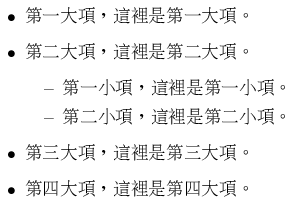
\includegraphics{itemize}
\end{quote}
\end{htmlonly}

\subsection{�C�|�����C���ҡ]enumerate�^}
\label{subsec:enume}\index{�C�|�����C���ҡ]enumerate�^}

�o�O�H�ƥئr�Φr����ù���Ʀr�Ӱ_�Y���ت����C�覡�C�P�˪��Ҥl�A�令 {\tt enumerate} ���ܡA�|�ƪ����G

%begin{latexonly}
\begin{quote}
\begin{enumerate}
\item �Ĥ@�j���A�o�̬O�Ĥ@�j���C
\item �ĤG�j���A�o�̬O�ĤG�j���C
  \begin{enumerate}
  \item �Ĥ@�p���A�o�̬O�Ĥ@�p���C
  \item �ĤG�p���A�o�̬O�ĤG�p���C
  \end{enumerate}
\item �ĤT�j���A�o�̬O�ĤT�j���C
\item �ĥ|�j���A�o�̬O�ĥ|�j���C
\end{enumerate}
\end{quote}
%end{latexonly}

\begin{htmlonly}
\begin{quote}
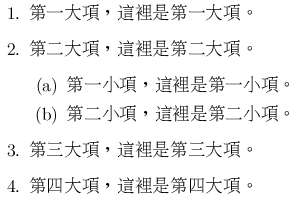
\includegraphics{enumerate}
\end{quote}
\end{htmlonly}

\subsection{�ԭz�����C���ҡ]description�^}
\index{�ԭz�����C���ҡ]description�^}

�o�O�H�@��²�u��r�ԭz�Ӱ_�Y���ت����C�覡�C�A��L�令 {\tt description} ���ܡA�L�O�H�����r�Ӱ_�Y���ت��A�o�Ǥ�r�n�Τ�A���A���C

\begin{quote}
\begin{verbatim}
\begin{description}
\item[�Ĥ@�j��] �o�̬O�Ĥ@�j���C
\item[�ĤG�j��] �o�̬O�ĤG�j���C
  \begin{description}
  \item[�Ĥ@�p��] �o�̬O�Ĥ@�p���C
  \item[�ĤG�p��] �o�̬O�ĤG�p���C
  \end{description}
\item[�ĤT�j��] �o�̬O�ĤT�j���C
\item[�ĥ|�j��] �o�̬O�ĥ|�j���C
\end{description}
\end{verbatim}
\end{quote}

�ƪ��X�Ӫ����G�O�G

%begin{latexonly}
\begin{quote}
\begin{description}
\item[�Ĥ@�j��] �o�̬O�Ĥ@�j���C
\item[�ĤG�j��] �o�̬O�ĤG�j���C
  \begin{description}
  \item[�Ĥ@�p��] �o�̬O�Ĥ@�p���C
  \item[�ĤG�p��] �o�̬O�ĤG�p���C
  \end{description}
\item[�ĤT�j��] �o�̬O�ĤT�j���C
\item[�ĥ|�j��] �o�̬O�ĥ|�j���C
\end{description}
\end{quote}
%end{latexonly}

\begin{htmlonly}
\begin{quote}
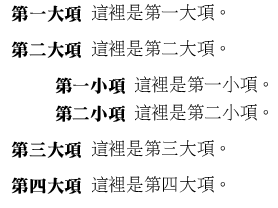
\includegraphics{description}
\end{quote}
\end{htmlonly}

�n�`�N���O�A���ޭ��@�ت����C���ҡA�C�Ӷ��ء]item�^����r�ԭz�|�۰ʧ��A�o�۷���K�A�ϥΪ̥u�n����C�����c�˧��A�M�ߥ��C�Ӷ��ت����e�N���F�C�ӥB�A�p�G�ϥΤ�A���A���@�Ǧr���B�r��βŸ��A���a�Y���ХܱN�|�O�o�Ǧr���B�r��βŸ��A�p�G�O�C�|�������C�覡�A���򦳤�A�����N���Q�s���A�|�۰ʸ��L�A�s�����ǫh�|�۰ʶ����C

%\section{enumerate �����M��}

%\subsection{���C���Ҥ����Ŷ�����}


\section{�u��}
\index{�u��}

�u�ئb�ƪ��W�����@�w���a��A�]���L�i�H�Ϲj���P���Ŷ��A�]�i�H���Y�dz�������X�ӡC���O�A�L�h���u�ؤ]�O�|���ٻ��ܥD�����n�Ƨ@�ΡA�ϥΤW�i��n�A�i�Ӥ�C�o�̧ڭ̭n�ͪ��O��ª��u�ءA����\index{����}�]�O�u�ت��@�����ΡA�ڭ̱N�|�b�� \ref{ch:graphic} ���A�A�ӽͪ��檺�B�z�C

%�b \LaTeX\ ���u�إi�����T�ءGLR�BRule �� Par�C

%\begin{quote}
%\begin{tabular}
%�u�غ��� & �N�q \\
%\hline
%LR  & left-right�A�u�ؤνu�ؤ������e�ѥ��ܥk \\
%Rule & 
%Par
%\end{tabular}
%\end{quote}

\subsection{���u�]rule�^}
\index{���u�]rule�^}

���u�]�O�ݩ��ت��@�ءA�N�O�@�ӹ������ΡA�u���L�A�L�����μe�]�u���ղӡ^�u���@�I�I�A�ҥH�A�ݰ_�ӴN�@�����u�}�F�C

\begin{quote}
\begin{verbatim}
\rule[�W�U��m(���)]{�e}{��}
\end{verbatim}
\end{quote}

�e�ΰ��������h�������A���ӤW�U��m�O����O�H�o�ӤW�U��m�O�M��u�]baseline�^\index{��u}\index{baseline}�b������A�p�G�S�����w�A���N�O�b��u����m�A�p�G�����w�A�N�̥��t�Ƚվ�M��u���۹��m�A���ȥѰ�u�V�W�վ�A�t�ȫh�Ѱ�u�V�U�վ�C�o�̨Ӭݭӭӹ�ҴN�A�ѤF�G

\begin{quote}
\begin{verbatim}
% example13.tex
\documentclass{article}
\parskip=3pt
\parindent=0pt
\begin{document}
This is a line.       % �e�� 1pt �e 3cm ����u�C
\rule{3cm}{1pt}
\rule[1ex]{3cm}{1pt}
\rule[-1ex]{3cm}{1pt}

\rule{1pt}{3cm}      % �e�� 3cm �e 1pt �����u�C

\rule{3cm}{0pt}TEST. % �� TEST �V�k�� 3cm�C

\rule{2cm}{3cm}      % �e�� 3cm �e 2cm �������ءC

\textcolor{blue}{This is color lines.}
\textcolor{red}{\rule{3cm}{1pt}}        % ���C�⪺�u�ءC
\textcolor{green}{\rule[1ex]{3cm}{1pt}}
\textcolor{blue}{\rule[-1ex]{3cm}{1pt}}
\end{document}
\end{verbatim}
\end{quote}

�sĶ�n���Ҥl�b�G

\begin{quote}
\url{http://edt1023.sayya.org/tex/latex123/example13.tex}\\
\url{http://edt1023.sayya.org/tex/latex123/example13.pdf}
\end{quote}

�ѨҤl���i�H�ݱo�X�ӡA�o�ӵe�u���O�ä��O����a�B��e�u�Ӥw�A�F���B�Ϊ��ܡA�i�H���X�\�h���P���ĪG�A�Ҧp����Ϥ������C

\subsection{��r���u�]underline�^}
\index{��r���u�]underline�^}

���ɭԧڭ̧Ʊ�b�Ѽg��r���P�ɡA�]�b��U�e�u�C\LaTeX\ ���{�������O�i�H�ϥΡA���N�O \verb|\underline{��r}|\index{underline@\verb=\underline=}�A�|�b��r���u�������P�ɵe�W�u���C���M�A�ϥΤW�`�`�|�M�{�b����u�d�V�A�]���ϥήɭn�S�O�d�N��ӭ����W�O�_�w�g�s�b�F�\�h��u�C

\subsection{��ء]box�^}
\index{box}

�o�̥D�n������r��ءAø�ϤW���@��اΦb�� \ref{ch:graphic} ���ɦA�ӰQ�סC�o�@�����}�Y�N�w�ͨ�A��g�峹�O�Ѥ@�ӭӪ� box �Һc�����A�o�̪���ثh�O�@�Ө嫬�� box�A�L���a��A���M�O�M�e���һ��� box �@�ˡA\TeX/\LaTeX\ �|��L�����@�ӳ�@���r���ӳB�z�C

�ڭ̥��Ӭݬݳ�²�檺��ت����O�G

\begin{quote}
\begin{tabular}{ll}
���O & �N�q�Χ@�� \\
\hline
\verb=\frame{��r}= & �N��r���e�H�i������خئ��A��ةM��r���S�����Z \\
\verb=\fbox{��r}=  & �N��r���e�H�i������خئ��A��ةM��r�����@�w���Z \\
\verb=\mbox{��r}=  & �@�ΩM \verb|\fbox| �P�A����ؤ��i��
\end{tabular}
\end{quote}
\index{frame@\verb=\frame=}\index{fbox@\verb=\fbox=}%
\index{mbox@\verb=\mbox=}

�H�W�����O���i�H�Φ���ؤ�r�C

��ؤ]���i�H�վ㪺���O�G

\begin{quote}
\begin{tabular}{ll}
���O & �N�q�Χ@�� \\
\hline
\verb|\framebox[�e��][����覡]{��r}| & �P \verb|\fbox| �P�A���i���w�e�פι���覡 \\
\verb|\makebox[�e��][����覡]{��r}| & �P \verb|\mbox| �P�A���i���w�e�פι���覡
\index{framebox@\verb=\framebox=}\index{makebox@\verb=\makebox=}
\end{tabular}
\end{quote}

�o�̪��e�׫����O��ت��e�סA�����w���ܡA�@�δN�p�P \verb|\fbox| �� \verb|\mbox| �@�ˡA�H�]����Ӥ�r�d�򬰼e�סA�ѩ�ڭ̤��e��������r���e���e�צ��h�֡A�]���e�ת����w�i�H�ϥΤU�C�۹��쪺�覡�G

\begin{quote}
\begin{tabular}{ll}
�e�� & �@�� \\
\hline
\verb|\width| & �o�Ӽe�״N�O \verb|\fbox| ����ɪ���ؼe�� \\
\verb|\height| & �o�O���`��u�ܮس������� \\
\verb|\depth| &  �o�O���`��u�ܮة������� \\
\verb|\totalheight| & �o�O \verb|\height| �M \verb|\depth| ���`�M \\
\end{tabular}
\end{quote}

�Ҧp�A�ڭ̫��w \verb|2\width| �L���N��N�O�H \verb|\fbox| �]������r���e�ɡA���ؼe�ת��G���e�C�ѼƸ��Y������覡�A�i���U�C�X�ءG

\begin{quote}
\begin{tabular}{>{\tt }ll}
����覡 & �@�� \\
\hline
c & center�A��r����ؤ����A�o�O�w�]�� \\
l & flushleft�A��r����إ��� \\
r & ushright�A��r����إk�� \\
s & stretch�A��r�������������ؤ�
\end{tabular}
\end{quote}

�����w���ܡA���M�N�O����ؤ�����m�F�C�ڭ̤]�i�H���w�i����ت��u���ʲӡA�Τ�ةM��r�������j�Z���G

\begin{quote}
\begin{tabular}{ll}
���O & �@�� \\
\hline
\verb|\fboxrule=���| & ���w��ؽu���ʲ� \\
\verb|\fboxsep=���| & ���w��r�M�ؽt�����Z%
\index{fboxrule@\verb=\fboxrule=}\index{fboxsep@\verb=\fboxsep=}%
\end{tabular}
\end{quote}

�Ъ`�N�A�o���|�v�T \verb|\frame{}|�C�p�G�Q�S�O���m���ت���m�A�]�i�H�ϥ� \verb|\raisebox|\index{raisebox@\verb=raisebox=} ���O�G

\begin{quote}
\begin{verbatim}
\raisebox{�W�U��m(���)}[�`��][����]{��r���e}
\end{verbatim}
\end{quote}

�o�̪��W�U��m���N�q�M \verb|\rule| ���O���Y���@�ˡA�u���L�A�o�̪��W�U��m�@�w�n���w�A�S���w�]�ȡA�����w�|�sĶ���~�C�Фd�U�O�o�A��ؤ����M�O�٥i�H����ت��C�ڭ̲{�b�N�Ӭݤ@�Ӻ�X����ҡG

\begin{quote}
\begin{verbatim}
% example14.tex
\documentclass{article}
\parskip=3ex
\parindent=0pt
\begin{document}
\frame{This is frame.}
\mbox{This is mbox.}
\fbox{This is fbox.}

\framebox{This is a framebox with no argumant.}

\framebox[1.5\width]{This is a framebox.}

\framebox[1.5\width][l]{This is a framebox with \texttt{l}.}

\framebox[1.5\width][r]{This is a framebox with \texttt{r}.}

\framebox[1.5\width][s]{This is a framebox with \texttt{s}.}

This is baseline.
\raisebox{3ex}[5\height]{This is a raisebox which lift 3ex.}

This is baseline.
\fbox{\raisebox{-3ex}[5\height]{This is a raisebox which lift $-$3ex.}}

\fboxrule=1.5pt
\fboxsep=8pt
\framebox[1.5\width][s]{This is a framebox with \texttt{s}.}
\end{document}
\end{verbatim}
\end{quote}

�o���L�ݦh�[�����A�sĶ�n���Ҥl�b�G

\begin{quote}
\url{http://edt1023.sayya.org/tex/latex123/example14.tex}\\
\url{http://edt1023.sayya.org/tex/latex123/example14.pdf}
\end{quote}

\subsection{�q�����}
\index{�q�����}

�t�~�A�]���Ω�q����r����ءA�i�H����Y�Ӭq���X�{�b�Y�S�w���Ŷ��B��m�C�ڭ̱`�`��o�ئw�ƺ٬��g�A�����A�⪩�����e�m��@�Ӥ��i������ط����A���M�A�o�Ӥ�ةM�@�몺 box�A�Ҧp�r���A���M�B��P�˪��a��A\LaTeX\ �|��L�����@�Ӧr�����ӳB�z�C

\begin{quote}
\begin{verbatim}
\parbox[����覡][����][�����m]{�e��}{��r���e}

\begin{minipage}[����覡][����][�����m]{�e��}
  �q�����e
\end{minipage}
\end{verbatim}
\end{quote}
\index{parbox@\verb=parbox=}\index{minipage@\texttt{minipage}}

�o�̪��Ĥ@�ӿ�ܩʰѼơu����覡�v�G

\begin{quote}
\begin{tabular}{>{\tt }ll}
t & top�A�q����ت��W�u����@�檺��u \\
b & bottom�A�q����ت��U�u����@�檺��u \\
c & center�A�q����ت���������@�檺��u�A�o�O�w�] \\
\end{tabular}
\end{quote}

\verb|\parbox| ���O�q�`�Ω���u����r���e�A�p�G�O�������q���A���ϥ� {\tt minipage} ���ҷ|�����K�C�o�Ǭq����ةM�W���ҽͨ쪺�@�Ǥ�س̤j�����P�O�A�q����إ��N�O�Ψӱƪ��p�q����y�A�]���L�|�M�@�륿�`�峹�q���@�˪��B�z�A�Ҧp�L�|�۰��_��A�I��ťզ�]�|�_�s�q���A���U�q���w�]�O���Y�ƪ��A�ӥB�A�b�w�ƤW�|��@�몺�q�����A�@����t�����Z�|�Y� 0pt�C

���פ��h���w���ܡA���N�O�H��Ӫ����g�_��B�z��A��Ӥ�r�q���ҧΦ������סC�ܩ󤺤��m�����]�O \texttt{t, b, c} �o�ǡA�N��O��r�q���b��ؤ����W�U��m�A���M�A�o�n�����w��ذ��׮ɤ~�|���N�q�A�]���A�u�����m�v�M�u���סv�O�n�P�ɫ��w���A�n�D�`�`�N���O�A�p�G���w�F���סA���S�����w�����m�A�h�w�]�O����e���ϥΪ��u����覡�v�ҫ��w���ѼơC

�o�ǰѼƪ��ϥη|���ǷнơA���o�O�u�ʩұa�Ӫ��u���n���c�v�A�����h���O�A�u���b�Ĥ@����IJ�ɧ�L�d�M���N���F�A��ڭn�Ψ�ɦA�Ӭd�L���ԲӰѼơA�`�Ϊ����O�B���ҡA�j���h�d�X���N�۵M�ӵM���O�_�ӤF�C


% ``�j�a�Ӿ� LaTeX'' LaTeX ��Z class.tex
% Copyright (c) 2004  Edward G.J. Lee <edt1023@info.sayya.org>
%
% �b���H�� GNU Free Documentation License 1.2 �ΥH�᪺�����W�d���U�A
% ���\�����B���G�έק�C���쪩�v�B���v�n�����o�����C
%
% �����G�����A�t�� fdl.tex�A���e�� GNU FDL ���W�d���C�p�G�򥢡A�i��
% http://www.gnu.org ���o�A�μg�H�ܦۥѳn�����|(Free Software Fundation)
% �����C
% 9 Temple Place - Suite 330, Boston, MA 02111-1307, USA.
%
% $Id: class.tex,v 1.14 2004/03/06 17:17:55 edt1023 Exp $
%
\chapter{\LaTeX\ ���зǤ�Z���O}
\label{ch:class}\index{��Z���O}

�o���D�n�O�b���� \LaTeX\ ��Z�����O�]document class\index{document class}�^\footnote{�o�b�ª������٬� style�A�o��ӵ��N�q�W�t���h�A�o�dz��O \TeX\ �����X�Ӫ������w�q�A�M���Ψөw�q�峹���j���c�A�H�K²�ƨϥΤW�Τ�Z�����e�C}�A�o�O \LaTeX\ �W�d��Z���鵲�c����k�C�ϥ� class ���ηN�A�N�O�⪩�����c�B�z�M��ڤ�Z���}�A�o�˪��̤j�n�B�N�O������g�峹�ƪ����c�W���@�P�ʡA�]�Ϥ�Z���e��M�n²��A�ϥΪ̥u�n�M�ߩ��Z���e���g�@�Y�i�A�p�G class �w�q���n�A�]�i�H�F��@��h�ܤƤS���ܧ��Z���e���ت��A�u�n��ޥΪ� class �����O���N�i�H�F�A��L���i�H������ʡC

�ثe�A\LaTeX\ �����ؼз����O�Ω�@����A�i�Ω�@�몺�ѫH�B���x�B���Z�B���i�νפ�C�����Ǵ��Z�B�פ�|�n�D�@�w�����c�A�o�ɱo�̻ݨD�t��q�w�C�]���A�]����L�����O�s�b�A�з����O�ä��O�ߤ@���C�ƦܡA�]�i�H�ۦ漶�g�ۤv����Z���O�C���M�A�ڭ̤@��ϥάO���ݭn�o�����s�A�o�̥u���� \LaTeX\ ���з����O�C�ӥB�A�p�G���M�L�H�洫��Z���ݨD�ɡA�ڭ����Ӻɥi�઺�ϥάy�q�ʸ��s�x�����O�C

�t�~�A�]���@�ǬO���� \LaTeX\ �������� macro\index{macro} �g�@�ɭn�Ψ쪺���O�A�o�Ǥw�W�X���g�峹���d��C

\section{\LaTeX\ ���O���ŧi}
\index{���O���ŧi}

\LaTeX\ �����O�A�n�b��Z���@�}�Y�ɴN�ŧi�]���M�A��W�����ѬO�S�����Y���^�A�L���@��榡�p�U�G

\begin{quote}
\begin{verbatim}
\documentclass[��ܩʰѼ�]{���O}
\end{verbatim}
\end{quote}
\index{documentclass@\verb=\documentclass=}

��ܩʰѼƬO�i�H�ٲ����A�����O�W�٫h����١A�@�w�n���w�@�����O�C�ӥB�u��u���@�����O�C

\section{���O����ܩʰѼ�}

��ܩʰѼƥi�H��ܦh�ӡA�U�ӿﶵ�O�H�r�I���}���C

\begin{enumerate}
\item {\tt 10pt, 11pt, 12pt}\\
���w����@�륿�`�r���j�p�A�w�]�O {\tt 10pt}�C��L�I�ƨS���~�� package ������������w�C
\item {\tt a4paper, letterpaper, b5paper, executivepaper, legalpaper}\\
���w�ȱi�j�p�A�w�]�O {\tt letterpaper}�C
\item {\tt fleqn} \\
�ϼƾǦ��a������A�w�]�O�~������C\index{fleqn@\texttt{fleqn}}
\item {\tt leqno} \\
�ϼƾǦ��s���a���A�w�]�O�a�k�C
\item {\tt titlepage, notitlepage}\index{titlepage@\texttt{titlepage}}\index{notitlepage@\texttt{notitlepage}} \\
�M�w title page �O�_�W���@���C�w�] \texttt{article}\index{article@\texttt{article}} ���W���@���A�� \texttt{report/book}\index{book@\texttt{book}}\index{report@\texttt{report}} �h�|�W���@���A�b�o�̬O�i�H���w���ܧ�w�]�欰�A�Ҧp \texttt{article} ��Z�A���w \texttt{titlepage} ���ܡA�� title page �N�|�W���@���C
\item {\tt onecolumn, twocolumn} \\
�峹����Ψ��榡�A�w�]�O����A�]�N�O������C\index{onecolumn@\texttt{onecolumn}}\index{twocolumn@\texttt{twocolumn}}
\item {\tt twoside, oneside}\index{twoside@\texttt{twoside}}\index{oneside@\texttt{oneside}} \\
�O�_�Ϥ��_���ƭ��C�w�] \texttt{article/report} ���Ϥ��A\texttt{book} �h�|�Ϥ��C�@�몺���y�A�b�˭q�������A�L�������u�٬��ѯ�A���ƭ��|�b���}���y�ɪ�����A�ӥB�䤤���e�|���V�ѯ᪺�����]���ɬO�V�k�^�A�Ϥ��A�_�ƭ��|�b�k�A���e�@�˷|�����V�ѯ�A�b \texttt{oneside} �����Ϋh�����o�˪��Ϥ��A���ީ_�������|�b�ȱi����������C
\item {\tt landscape} \\
��V�C�L���a�V�C�L�A�w�]�a�V�]portait�^�C\index{landscape@\texttt{landscape}}\index{portait@\texttt{portait}}
\item {\tt draft}\index{draft@\texttt{draft}} \\
��Z���sĶ�A�o�ɹ��ɱN���|�Q�ޤJ�A�i�[�ֽsĶ���t�סC���L�A�p�G�sĶ�O�ϥΦV�q�r�����ܡA�sĶ�t�����ӬO�ٺ�ܧ֡C���ϥ� {\tt draft} ���@�Ӧn�B�O�A�L�����a��|�ХܥX�ӡC
\item {\tt openright, openany}\index{openright@\texttt{openright}}\index{openany@\texttt{openany}} \\
�o�O�b����A�����}�l�O�_�O�_�ƭ��]right-hand page�^\index{�_�ƭ��]right-hand page�^}�C�b \texttt{book} ���O�A�w�]���|�q�_�ƭ��}�l�Areport ���O�h���|�C\texttt{article} ���O�S�����A�ҥH�A�惡�@�]�w�|�����C
\end{enumerate}

\section{���O������}

�o�̥u�C�X�@��峹�ϥΪ����O�A��L�S�������� \LaTeX\ �������ҨϥΪ����O�N���C�X�F�A�@��ϥΡA�o�����O�N�����F�C

\begin{quote}
\begin{tabular}{>{\tt }lll}
���O & �@��γ~ & �S�� \\
\hline
article & �@��u�� & �L���A�s�򭶤覡���w�ơA�L�_���ƭ����Ϥ� \\
report  & �����פ� & ���|�_�s���A�w�]�L�_���ƭ����Ϥ� \\
book    & ���y��   & ���|��_�ƭ��_�s���A�w�]�����ƭ����Ϥ� \\
letter  & �H��     & �^��H��榡 \\
slides  & �ۿO��   & �X�G�t�Υ~�ӮM����N \\
minimal  & ���դμg�s���O   & �o�O��²�檺���O�A�u�W�w�F���媺�e�B���A���`�r
\end{tabular}
\end{quote}
\index{article@\texttt{article}}\index{report@\texttt{report}}%
\index{book@\texttt{book}}\index{letter@\texttt{letter}}%
\index{slides@\texttt{slides}}\index{minimal@\texttt{minimal}}

���M�A�o�ǥγ~�ä��O�T�w���ܪ��A�o�ݨϥΪ̪��w�ơA���Q�h��ɶ��B�믫���ܡA���N�� \LaTeX\ �w�]���榡�h�ϥΡA�ܤִN���|�����СC�䤤 \texttt{minimal} class �O�ΨӴ��եΪ��A�Ϊ̼g�s�� class �Ϊ��A�L�����S���������w�ơA�Ҧp�A�S�����`�����c�A�U�ض��Z�]�S���w�q�A�w�]���r���O���`�r�A�S����L���ܤơA�X�G�Ҧ����ܤƭn�ۦ�h�w�q�C


% ``�j�a�Ӿ� LaTeX'' LaTeX ��Z package.tex
% Copyright (c) 2004  Edward G.J. Lee <edt1023@info.sayya.org>
%
% �b���H�� GNU Free Documentation License 1.2 �ΥH�᪺�����W�d���U�A
% ���\�����B���G�έק�C���쪩�v�B���v�n�����o�����C
%
% �����G�����A�t�� fdl.tex�A���e�� GNU FDL ���W�d���C�p�G�򥢡A�i��
% http://www.gnu.org ���o�A�μg�H�ܦۥѳn�����|(Free Software Fundation)
% �����C
% 9 Temple Place - Suite 330, Boston, MA 02111-1307, USA.
%
% $Id: package.tex,v 1.21 2004/03/07 12:18:40 edt1023 Exp $
%
\chapter{�����M��}
\label{ch:package}\index{�����M��}

\LaTeX\ �t�Τw�g�n�[�S����s�A���dz����i��|�򤣤W��ڪ��}�B�A�ӥB���Ǥ��w�������w�q�A�g�L�j�a���ϥΡA�oı�ä��O���򪺶���A�ר�O�\�઺�j�Ƥ譱�A�]���o���ͽͦp��ޥΥL�H�w�g�g�n�������A�o�ܭ��n�A�ɶq�קK���ƻs�y���l�A�g \TeX/\LaTeX\ macro\index{macro} �i���O�ܱM�~���u�@�A�n�קK�}�a�F���骺���c�A�ҥH����ݬݦ����򥨶��M��i�H�ϥΡC

%�U�@�䤣��A�X�������M��A�γo�ǥ����M�󪺩w�q�����ũһݡA�o�ɧڭ̴N�o�ۦ�ק�w�q�A�ƦܬO���s�w�q�ӲŦX�һݡA�o�]�O�o�@���dzƱ��Q���@�ӥD�D�C���O�A���O�C�@�ӤH�����R�Ϊ��ɶ��h�Dz� \TeX/\LaTeX\ �������y���A�ҥH�o�̱��Q���H��ΡB²�檺�w�q��k���D�A�y�L�������w���ŦX�@��ϥΪ���h�A�]�M�o�g�峹���c�Q�d�򤣲šC

\section{�@��M�󪺨ϥ�}

�ڭ̴��b�� \ref{subsec:preamble} �p�`�A�� \pageref{subsec:preamble}�A����L²�楨�����ޥΡA�ƹ�W�A���ǥ����t���\�h���ѼƨӰ��L�աA���O�C�ӥ����M�󪺰ѼƳ����|�@�ˡA�]���A�ϥήM�󤧫e�n���ݤ@�ݥL�Ҫ��W���ϥΤ�U�C�X�G�j�����������M�󳣦��ϥΤ�U�A�p�G�O�t�ΤW�N���������A����o�Ǥ��q�`�|��b�G

\begin{quote}
\begin{verbatim}
$TEXMF/doc  => Unix-like �t��
$TEXMF\doc  => DOS/Windows �t��
\end{verbatim}
\end{quote}

�o�ǥؿ����U�A�o�Ǥ��|����l \TeX/\LaTeX\ ��Z�A�]���sĶ�n�� \texttt{*.dvi} �� \textsc{PostScript}\index{PostScript@\textsc{PostScript}} �ɥi�H�\���A���D��K���ܡA�i�H�N�L���ন pdf �榡�Ӿ\���A��]�O�i�H�H����r�ӷj�M����A�b�d���O�B���Үɷ|�����K�C�b Unix-like\index{Unix-like} �t�Ω� Windows\index{Windows} �U�� cygwin\index{cygwin} ���Ҫ��ܡA�i�H�ϥ� \texttt{texdoc}\index{texdoc@\texttt{texdoc}} �o�ӫ��O�Ӿ\���A�Ҧp�G

\begin{quote}
\begin{verbatim}
texdoc amsguide  => �\�� amsguide.dvi �o���ɪ�����
texdoc -s ams    => �d�t�ΤW�Ҧ��t ams �r�˪����
\end{verbatim}
\end{quote}


\section{\LaTeX\ �x���󤤪��зǥ����M��}

���U�O \LaTeX\ �x���󤤩Ҫ����зǥ����M��C���M�O�зǥ����M��A���@�뱡�ΤU�A�ϥγo�� packages �����|�ä��h�A���O���S���ݭn�ɤ~�|�ޤJ�C

\subsection{alltt}\index{alltt@\textsf{alltt}}

�o�ӥ����M�󴣨� \texttt{alltt}\index{alltt@\texttt{alltt}} ���ҡA�M \texttt{verbatim}\index{verbatim@\texttt{verbatim}} ���Ҫ��@�άۦP�A�u�O \textbackslash{}�A\{�A\} ���@�ΩM�@��峹���ۦP�|�Q \LaTeX\ ��Ū�C�o������ΩO�H�o�ˤ@�� \LaTeX\ �o�ӯS���лx�]�i�H�ϥΡA�]�i�H�����Ҥ�����r�㦳�C��A�ΰ���L�ܤơA���M�A���Y����r�w�]���M�O�ϥΥ��r���r��\index{���r���r��}���C

\subsection{doc}\index{doc@\textsf{doc}}

�o�O�ΨӼg \LaTeX\ ��󪺥����M��A�o�b�ϥ� \texttt{ltxdoc}\index{ltxdoc@\texttt{ltxdoc}} �o�� class ���P�ɴN�|���J \textsf{doc} package�C�ѩ�o���O�Ω�@�몺���ϥγ��X�A�ҥH�A�o�̴N���h�͡A�����쪺�ܥi�ۦ�ѦҥL����󻡩��C

\subsection{exscale}\index{exscale@\textsf{exscale}}

�ѩ����� Computer Modern font\index{Computer Modern font} �����ƾǩ����Ÿ��]\texttt{cmex}\index{cmex@\texttt{cmex}}�^�u�� 10pt �j�p���r���]\texttt{cmex10}�^�A�����j�� \texttt{large} �H�W���r���ɡA�Ҧp��j�� \texttt{Large} �ɡA���ǼƾDzŸ����M�|�����@�w���j�p�A�o�ɥi�H�ϥγo�ӮM��A���o�ǼƾDzŸ��]��۩�j�A�Ҧp�n���Ÿ��C\textsf{exscale} �u���r���Y�񪺩w�q�A�]���u�n��o�ӮM��b preamble\index{preamble} �ϤޥδN�i�H�F�A�L�ݥ�����O�C

���L�A�o�̭n�����@�U�A�b \TeX/\LaTeX\ �̦r����j�A���ɥi��|�y�����{���u�����ΡA�ר�O�ƾǦ��l�A���F�U�μƾǦ��l���U�Ӧr�������Ŷ��w�ơA\texttt{cmex10} ���]�p�ä��A�X���ө�j�A�i�H�� \texttt{cmr5} ��j�� 10pt �M�u���� \texttt{cmr10} �Ӥ���N�|���D���{�X�ӷ|���@�ˡA�]���A�p�G�Ҽ{��T�t�X�����D�A��j�ƾǦ��l���r���ɥi��n�Ҽ{�@�U�ϥγ��X�A�ר�ثe�ĥΦV�q�r��O�p���C�иոեH�U���Ҥl�A�ڭ̧� \texttt{cmr5}�B\texttt{cmr10} �� \texttt{cmr12} �P�˩�j�� 30pt �Ӭݬݵ��G�|���|�@�ˡG

\begin{quote}
\begin{verbatim}
% test-fonts.tex
\font\largecmr=cmr12 at 30pt
\largecmr
This is cmr12 at 30pt.

\font\largecmr=cmr10 at 30pt
\largecmr
This is cmr10 at 30pt.

\font\largecmr=cmr5 at 30pt
\largecmr
This is cmr5 at 30pt.
\bye
\end{verbatim}
\end{quote}

�Ъ`�N�A�o�O \TeX\ ��Z�A���O \LaTeX\ ��Z�A�ҥH�n�ϥ� \texttt{tex}\index{tex@\texttt{tex}} �� \texttt{pdftex}\index{pdftex@\texttt{pdftex}} �ӽsĶ�A�L�����G�p�U�A�j�a�i�ܲM�����ݱo�X�ӡA���M�P�ˬO�V�q�r�A����j�ɪ����{�ä��|�@�ˡG

\begin{quote}
\url{http://edt1023.sayya.org/tex/latex123/test-fonts.tex}\\
\url{http://edt1023.sayya.org/tex/latex123/test-fonts.pdf}
\end{quote}

�ھ� Knuth\index{Knuth} �б·���]�p \MF\index{metafont@\MF}�A�L���z���O�@�ӦP�˪��r���b��j���ɭԡA�P�@�Ӧr�A�L�������m�񪺬۹��m���ӭn�H��j�����Ʀӵy�[�վ�C�]���A���p�ڭ̥u�ϥΤ@�ئV�q�r��\index{�V�q�r��}�A�Φb���P����j���v���ɭԡA��r�Ÿ������Ŷ��t�X�|���ͤ��@�˪����G�A�ר�O�Φb�ƾǦ��l\index{�ƾǦ��l}���ɭԡA��[����C

���M�A��ΤW \MF\ ���M�]�O�@�ئV�q�r���A���ѩ�ӹL������A���A�X���ӿù���ܤW�ΡA�ҥH�~�|�h�ӨD�䦸�A�ন pk �I�}�r���ӨϥΡC�o�]�N�O������P�ˬO \texttt{cmr} ���r���A�|���X�ؤ��P�I�ƪ��W�ߦr������]�A�a�ϬO�V�q�r�]�O�p���C\TeX\ �w�g 20 �X���F�A���O�A�ڭ̪��r���޳N���G�٬O�S���������W���� Knuth �бª��z���C

\subsection{fontenc}\index{fontenc@\textsf{fontenc}}

�b�� \ref{subsec:font-attr} �p�`�A�� \pageref{subsec:font-attr}�A������r���s�X�����D�C�n���ܦr���s�X�A�i�H�ϥγo�� \textsf{fontenc} package�C�H T1 font encoding\index{T1} �ӻ��G

\begin{quote}
\begin{verbatim}
  ...
\usepackage[T1]{fontenc}
  ...
\end{verbatim}
\end{quote}

�o�˴N�i�H�F�A���ѩ�@�Ǧr���A�Ҧp�ڬw�r���A�b��Ӫ� Computer modern Type1 �r�����w�Ƥ��@�ˡA�ҥH�A���dz����|�ϥέ�l�� \MF\ �r�����ഫ���� pk �I�}�r�A�o�˪��ܡA�@��L�����L�X�ӬO�t�����j�A���p�G�O�Q�s�@�� PDF �榡�b�å����\�����ܡA�r�������{�|�ܱo����C�z�Q���ܡA�n�w�� \texttt{cm-super}\index{cm-super@\texttt{cm-super}} Type1 �r���A���O�@��ϥΪ̮��Ȧۦ�w�˦r���|���x���C�o�b te\TeX\ 2.x\index{tetex@te\TeX} �H�᪺�����A�w�g�����W \textsf{pxfonts}\index{pxfonts@\textsf{pxfonts}} �� \textsf{txfonts}\index{txfonts@\textsf{txfonts}} package �Ψ�r���A�ҥH�A�p�G�O�s�񪩥��� te\TeX\ ���ܡA�i�H�ѥH�U���覡�ӨϥΡG

\begin{quote}
\begin{verbatim}
  ...
\usepackage{txfonts}
\usepackage[T1]{fontenc}
  ...
\end{verbatim}
\end{quote}

�䤤 \textsf{txfonts} �O���� Times �t�C���r���A\textsf{pxfonts} �O���� Palatino �t�C���r���C���M�A�o������r�������D���I�����A�o���b�o�g�峹���Q�׽d��A�u�వ²�檺�����A�p�G�S���S���ݭn�A�Ҧp�A�ڬw�r���B�@�Ǧ������Ÿ����r���A���ϥιw�]�� OT1 �s�X�N��F�A�]���o�ǮM��Ҫ������Ǧr���A�u���@�ؤj�p�� Type1 �r���b�Y��A�]���ϥΤW���ȷ|�����u\index{���u}�����ΡC

\subsection{graphpap}\index{graphpap@\textsf{graphpap}}

�o�O���ͤ��Ȫ������C�L���ѤF�@�ӫ��O�A�i�H�e���A�i�H�t�X \texttt{picture}\index{picture@\texttt{picture}} ���ҨӨϥΡA�L���y�k�O�G

\begin{quote}
\begin{verbatim}
  ...
\usepackage{graphpap}
  ...
\graphpaper[n](x,y)(x1,y1)
  ...
\end{verbatim}
\end{quote}

�䤤�� \texttt{n} �p�G�ٲ����ܡA�w�]�O 10�A�L�����O���Ȫ��̤p��׳��C\texttt{(x,y)} �� \texttt{(x1,y1)} �����O���U���Υk�W�����y�ЭȡA�Ҧp�G

\begin{quote}
\begin{verbatim}
\documentclass{article}
\usepackage{graphpap}
\begin{document}
\graphpaper(0,0)(360,360)
\end{document}
\end{verbatim}
\end{quote}

�o�˷|�e�X�H 10 ���̤p��ת����A�sĶ�n���Ҥl�p�U�G

\begin{quote}
\url{http://edt1023.sayya.org/tex/latex123/test-graphpap.tex}\\
\url{http://edt1023.sayya.org/tex/latex123/test-graphpap.pdf}
\end{quote}

\subsection{ifthen}\index{ifthen@\textsf{ifthen}}

\TeX\ �����O�@�رƪ��{���y���A���M�|������P�_��\index{����P�_��}�Ӥ�K�g�����A���p�G��Z���]�R���F����P�_���A�N�|�Ϥ�Z�����ơA���H�\Ū�B���@�A�]���A�@�����P�_���j�h�ƨϥΦb�����w�q�A�Ӥ��O�g�b��Z�����C�o�� package �N�O�b²�Ʊ���P�_���A�H�K�]�i�H��K�ϥΦb��Z�����C 

\textsf{ifthen} package ���ѤF \verb|\ifthenelse|\index{ifthenelse@\verb=\ifthenelse=} ���O�Ӱ�����P�_�C�L�᭱���T�ӰѼơA�Ĥ@�ӬO���󦡡A�ĤG�ӬO���󬰯u���ɭԭn���檺���e�A�ĤT�ӬO���󬰰����ɭԭn���檺���e�C�o�̤��h�ͥL���ϥΡA���U�u���Ѥ@�ӹ�Ҥ��q�G

\begin{quote}
\begin{verbatim}
  ...
\usepackage{ifthen}
  ...
\ifthenelse{\isodd{\thepage}}%
  {\setlength{\leftmargin}{10pt}}%
  {\setlength{\leftmargin}{0pt}}
  ...
\end{verbatim}
\end{quote}

�o�˩_�ƭ��ɡA\texttt{leftmargin} �|�]�� 10pt�A���ƭ��ɫh�� 0pt�C�᭱�[ \texttt{\%} �N���A�o�T��O�@���A�䶡�S���ťաC

\subsection{inputenc}\index{inputenc@\textsf{inputenc}}

�ѩ� \textsf{fontenc} package ���@�Ǧr���s�X�w�ơA�M�@��ҿת� Latin-1\index{Latin-1} �o�ǽs�X�]input encoding�^�A�L�̪����e���@�w�۲šA�ҥH�A\textsf{fontenc}\index{fontenc@\textsf{fontenc}} package �`�|�M \textsf{inputenc} package ���۰t�X�ϥΡA�H�T�O�b�ϥμڬw�r���B�Ÿ��ɯॿ�T���o��r�C�Ҧp�G

\begin{quote}
\begin{verbatim}
  ...
\usrpackage[T1]{fontenc}
\usepackage[latin1]{inputenc}
  ...
\inputencoding{ascii} % �]�i�H�b��Z�����ܴ�
  ...
\inputencoding{latin2}
  ...
\inputencoding{latin1}
  ...
\end{verbatim}
\end{quote}

���M�A�ڭ̪���Z�p�G�u�O�^���y�t���峹�A���o�dz��i�H�����z�|�C

\subsection{latexsym}
\label{subsec:latexsym}\index{latexsym@\textsf{latexsym}}

�o�O \LaTeX\ �B�~���Ѫ��Ÿ��C�b�s���� \LaTeXe\ �ä��|�۰ʸ��J�A�n�ۦ�ޤJ�o�ӿW�ߥX�Ӫ� package�C�o�D�n�O���� \texttt{lasy*} �o�Ǧr�����Y���Ÿ��C�p�G���ϥ� \textsf{amsfonts}\index{amsfonts@\textsf{amsfonts}} �� \textsf{amssymb}\index{amssymb@\textsf{amssymb}} package ���ܡA�o�� \textsf{latexsym}\index{latexsym@\textsf{latexsym}} �Ÿ����ӬO�i�H�L�ݤޤJ�]���ּƲŸ��O \LaTeX\ �S�����^�C�ܩ�U�زŸ��� package �����Ǥ��e�A�i�H�ѦҨt�ΤW�� \texttt{symbols*} �o���ɮסA�L�i��s�b���Φ��O�G

\begin{quote}
\begin{verbatim}
symbols.dvi
symbols-a4.ps[pdf]
symbols-letter.ps[pdf]
\end{verbatim}
\end{quote}

�Ϊ̡A�]�i�H�q CTAN\index{CTAN} �U���̷s�������G

\begin{quote}
\url{ftp://cam.ctan.org/tex-archive/info/symbols/comprehensive/symbols-a4.pdf}
\end{quote}

\subsection{makeidx}\index{makeidx@\textsf{makeidx}}

�o�O�b�s�@����\index{����}�ɭn�ޤJ�� package�A�ڭ̷|�b�� \ref{sec:index} �`�A�� \pageref{sec:index} �A�ӰQ�סC

\subsection{newlfont}
\index{newlfont@\textsf{newlfont}}

�o�O�����ª� \LaTeX\ ���r���Ϊk�A���L�ϥηs�����r��� package�C�]�N�O�ڭ̦b�� \ref{subsec:font-command}�A�� \pageref{subsec:font-command} �Ҵ��쪺�Ϊk�C���K�·СA�ڭ̺ɶq�קK�ϥ��¥Ϊk�A�ӨϥΦr�����зǫ��O�C

\subsection{oldlfont}
\index{oldlfont@\textsf{oldlfont}}

�o�O�����ª� \LaTeX\ ���r���Ϊk�� package�C

\subsection{showidx}
\index{showidx@\textsf{showidx}}

�o�� package �|��ܡA\verb|\index|\index{index@\verb=\index=} ���O�U�b����a��C�o�]�|�b�� \ref{sec:index} �`�ӰQ�סC

\subsection{syntonly}

\textsf{syntonly}\index{syntonly@\textsf{syntonly}} package ���� \verb|\syntaxonly|\index{syntaxonly@\verb=\syntaxonly=} ���O�A�L�i�H�ˬd�y�k�O�_���T�A�ä��|�� {\tt *.dvi} �ɪ���X�C���o�� \verb|\syntaxonly| ���O�@�w�n��b preamble �ϡC

\subsection{tracefnt}
\index{tracefnt@\textsf{tracefnt}}

�o�O�l�ܦr���ϥα��Ϊ� package�C�q�`�sĶ�ɩҲ��ͪ���T�w�g�ܨ����A���p�G�Ʊ榳��ԲӪ��r���ϥθ�T���ܡA�i�H�ϥγo�� package�G

\begin{quote}
\begin{verbatim}
  ...
\usepackage[debugshow]{tracefnt}
  ...
\end{verbatim}
\end{quote}

�Ъ`�N�A�o�˷|�W�[�sĶ���ɶ��A�ӥB {\tt *.log} �ɷ|�ܤj�C

\section{\LaTeX\ �x���󤤪��u���}

�o�ǥ����M��A\LaTeX\ �x����O�k���b�����n��]relative software�^���A�i��|��W�@�`���쪺�зǥ����M��ӱo��ΨǡC���]�P�ɥi�H�ݱo�X�� \LaTeX\ �D���ت��M�󤣤֡A�[�W��L�~�Ӫ������M��A���u���O�M�󺡤ѭ��A�ڭ̫ܧƱ�b�i�઺���ΤU \LaTeX\ team �i�H�Ҽ{�N�@�ǥ��n���M��ǤJ���ءA��[���ꪩ���B�z�M��Z�g�@���}���z���C

\subsection{\AmS-\LaTeX}
\index{AmS-LaTeX@\AmS-\LaTeX}

\LaTeX\ �����N���ƪ��ƾǦ��l����O�A���b����M�~�ϥήɡA�i��|�ݭn�W�j�L���\��A\AmS-\LaTeX\ �O����ƾǨ�|�]American Mathematical Society, AMS\index{AMS}\index{American Mathematical Society}\index{����ƾǨ�|}�^�ҵo�i���@�ӼW�j \LaTeX\ �ƾǦ��l�s�誺�����աA�O�� \AmS-\TeX\\index{amstex@\AmS-\TeX} ���ӹL�ӵ� \LaTeX\ �ϥΪ��A�L�D�n������ӳ����G\textsf{amscls}\index{amscls@\textsf{amscls}} �� \textsf{amsmath}\index{amsmath@\textsf{amsmath}}�A�e�̴��ѲŦX AMS �����W�檺��Z���O�A��̥i�[�j��� \LaTeX\ ���ƾǼҦ��C�ڭ̷|�b�� \ref{ch:math} ���A�� \pageref{ch:math} �[�H���СC

\subsection{babel}
\index{babel@\textsf{babel}}

�p�G�Q�ƪ��^��H�~����L�ڬw��a���y��A�Ҧp�G�w��B�k��A���i�H�Q�� \textsf{babel} �����M��C

\subsection{cyrillic}
\index{cyrillic@\textsf{cyrillic}}

�o�O�M���ƪ����Ԥҥ��ڻy��A�Ҧp�G�X��A���i�H�ϥγo�ӮM��C

\subsection{graphics}
\index{graphics@\textsf{graphics}}

�o�O�B�z�ϧέn�Ψ쪺�����M��\index{�����M��}�C���ثe�@�볣�ϥΥ\��������� \textsf{graphicx}\index{graphicx@\textsf{graphicx}} �����M��Ө��N \textsf{graphics}\index{graphics@\textsf{graphics}} �F�A�ƹ�W�A�ޥ� \textsf{graphicx} �|�۰ʪ��ޥ� \textsf{graphics}�A�Ӧb���O�ϥΪ���K�ʤW�A\textsf{graphicx} ���ΡA�]���ڭ̩��᳣�O�H \textsf{graphicx} ���D�ӻ������C�o��ӮM���ݩ� \LaTeX\ ���ϧΤu��աA�o�Ӥu��ե]�A�F�M�C��B�ϧά������U�إ����A�ڭ̷|�b�� \ref{ch:graphic} ���A�� \pageref{ch:graphic} �ӰQ�סC

\subsection{psnfss}
\index{psnfss@\textsf{psnfss}}

�o�O Type1 �r���������M��աA�Ҧp�G\textsf{times}, \textsf{charter}, \textsf{mathptmx}\index{mathptmx@\textsf{mathptmx}} �����A�L�|�h�ϥγo�� Type1 �r��\index{Type1 �r��}�C���q�`�o�Ǧr�����\�h�O�ӷ~�r���A�t�ΤW���@�w�|���A�p�G�S�����ܡA�|�h�ϥ� free ���N���r���A�Ϊ̴N���O�J�o�Ǧr���F�C�p�G�S���o�ǰӷ~�r���A�S�Q�n�O�J���N�� Type1 �r�����ܡA�i�H�Ҽ{�ϥ� \textsf{txfonts} �� \textsf{pxfonts} �����M��Ψ�Ҫ��r���C���M�A�p�G�M�~�ϥΪ��ܡA�i��o�Ҽ{�ʶR�M�~���ӷ~�r���ӨϥΡC

\subsection{array}
\index{array@\textsf{array}}

�o�O�[�j��Ӫ� \texttt{array}, \texttt{tabular} ���Ҫ������M��A�i�W�\�h�ӳ��L�ժ��\��C�o�b�� \ref{sec:array} �`�A�� \pageref{sec:array}�A�ɷ|�Q�ר�C

\subsection{calc}
\index{calc@\textsf{calc}}

�o�ӮM��i�H�� \LaTeX\ �����@��²�檺�N�ƹB��C�D�n�Ω�L�դ@�ǭ�l�w�]�����פέp�ƾ��]counter\index{�p�ƾ�}\index{counter}�^�C

\subsection{dcolumn}
\index{dcolumn@\textsf{dcolumn}}

�o�O�����椤�㦳�p���I���Ʀr����������M��C�ڭ̷|�b�� \ref{sec:dcolumn} �`�A�� \pageref{sec:dcolumn} ���ԲӰQ�סC

\subsection{delarray}
\index{delarray@\textsf{delarray}}

�o�O�[�j \textsf{array}\index{array@\textsf{array}} �����M�󪺥\��A���x�}�Φ�C�����j���ɲŸ��i�H�ϥθ�²�檺���O�C�o�ӮM��n�t�X \textsf{array} �����M��ӨϥΡC�q�`�b \textsf{array} �����M�󤤡A�o�ǯx�}�Φ�C�����j���ɲŸ��O�� \verb|\left| �� \verb|\right| �Ӥ޾ɤ~�|�X�ӡA���ϥ� \textsf{delarray} �����h�����p���·СC�o�b�� \ref{ch:math} ���|�Q�ר�C

\subsection{hhline}
\index{hhline@\textsf{hhline}}

�o�ӥ����M��|��K�b�e��u�ɤ]�i�H���J���檺�a�u�C

\subsection{longtable}

\textsf{longtable}\index{longtable@\textsf{longtable}} �O�Φb�󭶪���C�q�`�b \LaTeX\ ���� \texttt{tabular} ����O�����@�� box\index{box} �ӳB�z�A�]���L�k�A���ΡA�ҥH�L�k�󭶨Ӫ��{�C�o�]�|�b�� \ref{sec:longtable}�A�� \pageref{sec:longtable} �ͨ����ɴ��ΡC

\subsection{tabularx}
\index{tabularx@\textsf{tabularx}}

�o�O \texttt{tabular}\index{tabular@\texttt{tabular}} ��������\index{��������}���[�j���A�L�i�H��K���ƪ����w�e�ת�����C�P�˪��A�o�|�b�� \ref{sec:tabular} �`�A�� \pageref{sec:tabular} �ɴ��ΡC

\subsection{afterpage}
\index{afterpage@\textsf{afterpage}}

�o�ӥ�D�n�b�վ� \LaTeX\ ���B�����ҡ]floating environment�^\index{�B������}\index{floating environment}�ɡA�m��B�ʪ���A�Ҧp�G�ϡB������m�C

\subsection{bm}

\textsf{bm}\index{bm@\textsf{bm}} ���N��A�N�O bold math(symbol)�A�o�|���ƾǦ��l�H���骺�覡����ܡC�o�ӥ����M��A���Ѥ@�� \verb|\bm{}| ���O�A�u�n��ƾǦ��l�m��j�A�����N�|�Ѳ������ܡC

\subsection{enumerate}
\label{subsec-enump}\index{enumerate@\textsf{enumerate}}

�o�O�[�j \texttt{enumerate}\index{enumerate@\texttt{enumerate}} �C�|�����C����\index{�C�|�����C����}�������M��C�L�i�H�ܤ�K�����w�n�ϥΤ���覡�Ӱ_�Y�A��l�� \texttt{enumerate} ���ҡA�w�]�Ĥ@�h�O���ԧB�ƥئr�A���M�]�i�ܧ�A���n���s�w�q�A���O�ܤ�K�C�o���|�ӨҤl�G

\begin{quote}
\begin{verbatim}
% example15.tex
\documentclass{article}
\usepackage{enumerate}
\begin{document}
\begin{enumerate}[Example-1.]
\item This is a item 1.
\item This is a item 2.
  \begin{enumerate}[(1)]
  \item This is a item (1).
  \item This is a item (2).
  \end{enumerate}
\item This is a item 3.
\item This is a item 4.
\end{enumerate}
\end{document}
\end{verbatim}
\end{quote}

�i�H���w�|������ܪ����G\texttt{A, a, I, i, 1}�A�p�G�o�ǬO�ݩ�T�w��ܪ������A�h�n�H�j�A���A�_�ӡA�_�h�L�|���ǭp����ܡC�иյ۩M�� \ref{subsec:enume} �p�`�A�� \pageref{subsec:enume} ���з� \texttt{enumerate} ���Ҥ���@�U�C�sĶ�᪺���G�p�U�G

\begin{quote}
\url{http://edt1023.sayya.org/tex/latex123/example15.tex}\\
\url{http://edt1023.sayya.org/tex/latex123/example15.pdf}
\end{quote}

�o�̽Ъ`�N�@�U�@�ǦP�W�����ҡB�����M��A�Ҧp \textsf{array} �����M��� \texttt{array} ���ҡA�o�̪� \texttt{enumerate} �����M��]�O�@�ˡC

\subsection{fontsmpl}
\index{fontsmpl@\textsf{fontsmpl}}

�o�O�r�� sample ���� package�A�L�i�H�O���ʪ��A�]�i�H�ޥγo�� package �᪽���ϥ� \verb|\fontsample| �o�ӫ��O�ӦL�X�ثe�ϥΪ��r�� sample�C

���ʪ��ܡA�n�ۦ��J�r�ڦW�١Csample �ɦb \texttt{\$TEXMF/tex/latex/tools} �ؿ��U�A�u�n�U�G

\begin{quote}
\begin{verbatim}
latex fontsmpl.tex
\end{verbatim}
\end{quote}

�N�i�H�F�A�L�|�X�{�G

\begin{quote}
\begin{verbatim}
This is TeX, Version 3.14159 (Web2C 7.4.5)
(./fontsmpl.tex
LaTeX2e <2001/06/01>
Babel <v3.7h> and hyphenation patterns for american, french,
german, ngerman, nohyphenation, loaded.
(/usr/share/texmf/tex/latex/base/article.cls
Document Class: article 2001/04/21 v1.4e Standard LaTeX document class
(/usr/share/texmf/tex/latex/base/size10.clo)) (./fontsmpl.sty)
Please enter a family name (for example `cmr').

\family=
\end{verbatim}
\end{quote}

�u�n��J�n���ժ��r���r�ڡA�Ҧp \texttt{cmr}�A�L�N�|���� \texttt{fontsmpl.dvi} �o���ɡA�M��N�i�H�ϥ� \texttt{dvips}\index{dvips@\texttt{dvips}} �� \texttt{dvipdfm[x]}\index{dvipdfmx@\texttt{dvipdfm[x]}} ��L�ন ps/pdf �榡���ɮסC�L�u�|���� OT1\index{OT1} �� T1\index{T1} ��ئr���s�X�C

\subsection{ftnright}
\index{ftnright@\textsf{ftnright}}

\LaTeX\ �b���榡�ƪ��]two-column mode�^\index{���榡�ƪ��]two-column mode�^}�ɡA�L���}���O�m��b�U����쩳���C\textsf{ftnright} �|�N���榡�ƪ��ɡA��Ҧ����}�����m��b�k�橳���C�o�˥i�H�N�}�������A�ݰ_�Ӥ��|�����áC

\subsection{indentfirst}

�q�`�A\LaTeX\ �����`�}�Y���Ĥ@�Ӭq���O���Y�ƪ��A�b�ĤG�Ӭq���_�~�|�Y�ơC�p�G�ߺD�C�Ӭq�������Y�ơA�i�H�ϥ� \textsf{indentfirst}\index{indentfirst@\textsf{indentfirst}} package�C�o�ӮM��]�O�ޤJ�N�i�H�F�A�L�ݥ�����O�C

\subsection{layout}
\index{layout@\textsf{layout}}

�o�O��ܥثe�����t�m\index{�����t�m}�� package�C�ޤJ�o�� package ��A�u�n�b����ϤU \verb|\layout| ���O�A�L�N�|�e�X�ثe�������t�m�A�]�|�N�U�ؼƾ���ܥX�ӡC�ڭ̦b�� \ref{subsec:layout} �p�`�A�� \pageref{subsec:layout}�A���Y����ܪ������ϡA�N�O�o�˵e�X�Ӫ��C


\subsection{multicol}
\label{subsec:multicol}\index{multicol}

�b \LaTeX\ �ŧi��Z���O���P�ɡA�ڭ̥i�H��� \texttt{twocolumn} �ӿ�ܨ��榡���ƪ��A�A�h�h����C�b���榡���ƪ��ɡA�ڭ̥i�H�ϥ� \verb|\onecolumn|\index{onecolumn@\verb=\onecolumn=} �� \verb|\twocolumn|\index{twocolumn@\verb=\twocolumn=} ���O�A�b����Ψ��涡�ܴ��A���o���@�ӫ��Y�������I�A���N�O����ܴ��]�|���ϴ��s���A��Ӫ������N�|��o���m�C

\textsf{multicol} ���ت��A���Ȭ�}����A�i�H���h�榡���ƪ��]�̦h�i�ܤQ�檺�ƪ��^�A�]�i�H�b�ܴ����s�Ʈɦb�P�@�����ܴ��A�Ӥ������s���C�L���ѤF \texttt{multicols}\index{multicols@\texttt{multicols}} ���ҨӰ���쪺�ܴ��C�L���ϥΤ�k��²��A���ƥؤ��ܴ����������Ҩӱ���G

\begin{quote}
\begin{verbatim}
  ...
\usepackage{multicol}
  ...
\begin{multicols}{���}
  ...
  ���e�A�̥��`����覡�Ѽg�Y�i
  ...
\end{multicols}
\end{verbatim}
\end{quote}

�Ъ`�N�A�ޤJ�� \textsf{multicol} �O�S�� `s' ���A�����Ҥ��� \texttt{multicols} �O�� `s' ���C\textsf{multicol} package �B�z�}�����覡�A�M����ƪ��ۦP�A�N�O�q�q�m�󥻭������A�������k���C

\subsection{rawfonts}
\index{rawfonts@\textsf{rawfonts}}

�o�O���� \LaTeX\ 2.09 �ª����C���r�����O�A�Ҧp \verb|\texrm| �N�� 10pt ��ù���r�ڪ��r�C�b�s���� \LaTeXe\ �èS���w�q�o�ǫ��O�C

\subsection{somedefs}
\index{somedefs@\textsf{somedefs}}

�o�O�g \LaTeX\ �������@�ǽd�ҩw�q�A�i�H�ܮe�������䤤�]�w�Ӽg�ۤv�� package�C�o���b�o�g�峹���Q�׽d��A�]���N���h�ͤF�C

\subsection{showkeys}
\index{showkeys@\textsf{showkeys}}

�o�� package �|�� \verb|\label|, \verb|\ref|, \verb|\pageref| ���椬�ѷӪ����O���e�A�Τ��m�ޥΤ��e�A�b���O�Ҧb�B�L�X�ӡC

\subsection{varioref}
\index{varioref@\textsf{varioref}}

�o�O�[�j�����椬�ѷ�\index{�椬�ѷ�}���覡�A�ڭ̷|�b�� \ref{ch:abook} ���ӰQ�סC

\subsection{verbatim}
\index{verbatim@\textsf{verbatim}}

�o�O�[�j \LaTeX\ ��Ӫ� \texttt{verbatim} ���Ҫ��P�W�M��C�i�H�b���Y�ϥε��ѡA�]�i�H�Q�� \verb|\verbatiminput{�ɮצW}|\index{verbatiminput@\verb=\verbatiminput=} ���O�ӤޤJ�~���ɮסA���M�A�ޤJ��|�۰ʶi�J \texttt{verbatim} ���Ҥ��C

\subsection{xr}

\textsf{xr}\index{xr@\textsf{xr}} �O eXternal References ���Y�g�A�N��N�O�椬�ѷӥ~�����ɮסC�o�|�b�� \ref{sec:ref} �`�A�� \pageref{sec:ref} �ӰQ�סC

\subsection{xspace}
\index{xspace@\textsf{xspace}}

�o�� package �|�b�@�ӥ����������o�������J�A�����ťաC�ڭ̦b�� \ref{gen:gamerules}�A�� \pageref{gen:gamerules}�A�ɴ��ͨ� \LaTeX\ ���O�����������D�A�ҥH�A�ڭ̱o�b���O��[ `\verb|\ |' �Ϊ� `\verb|{}|' �ӵ����@�ӫ��O�C���p�G�����w�q�ɨϥΤF \textsf{xspace} �����M�󪺤@�ӫ��O \verb|\xspace|�A����L�N�|�۰ʧP�_���O��ɵ����A�Ӥ����ۦ洡�J `\verb|\ |' �� `\verb|{}|' �F�C

\subsection{theorem}
\index{theorem@\textsf{theorem}}

�o�O \LaTeX\ ���ت� \texttt{theorem} ���Ҫ��[�j�������M��C�ڭ̷|�b�� \ref{ch:math}�A�� \pageref{ch:math}�A�A�ӰQ�סC


\section{�����M���B�M�H}
\label{sec:pkgwhere}

���Ƶo�����l�n�ɶq�קK�A�ҥH�A�p�G�ݭn�ǥ\��A�� \LaTeX\ ���G�S���A���i�H����ݬݬO���O�O�H�w�g���g�n�������\�઺�����M��A�����n�䪺���ӬO FAQ\index{FAQ} ���G

\begin{quote}
\url{http://www.tex.ac.uk/faq}
\end{quote}

�b \url{news://tw.bbs.comp.tex} �]���@�g Chun-Chieh Huang\index{Chun-Chieh Huang} �Һ��@������ FAQ\index{���� FAQ} �i�H�ѦҡC�t�~ \url{news://comp.text.tex} �h�O�^��Q�׸s�աA�i�H�h�h�Q�ΡC�p�G�w�g���D�M��W������r�A���i�H��G

\begin{quote}
\url{http://tug.ctan.org/CTANfind.html}
\end{quote}

�h�j�M�A�j�M���i�H���ӥؿ������Y�ɡC�q�`�A�w�� package�A�L���Y�|�����p��w�ˡA�U�@�S�����ܡA�i�H�� bbs/news �W�o�ݡA�Ϊ̤U���H�U�o�� sh script�G

\begin{quote}
\url{http://edt1023.sayya.org/tex/latex123/ltxins.sh}
\end{quote}

�L���ϥΤ�k��²��A��L�m�������|�i�Τ��B�G

\begin{quote}
\begin{verbatim}
ltxins.sh your.dtx(or your.ins)
\end{verbatim}
\end{quote}

�o�˴N��F�A�L�|���ͥ��n�� \texttt{*.sty} �� \texttt{*.tex} �� pdf �榡���������C�o���Y�ϥΪ��O \texttt{dvipdfm[x]}�A�ҥH�n���w�˳o��ؤu��~��C���M�A�L���|�۰ʦw�ˡA�A�٬O�n��ʧ�@���ɮ׫����� \LaTeX\ ��o�쪺�a��C�o�u�O�@�ӫ�²�檺�u��A�]�����O�үন�\�sĶ�X���X�ӡC

�p�G�Q���D�Y�ӮM��b�t�ΤW�O�_�w�w�ˡA�w�˦b����a��A�i�ϥΥH�U���p�u��G

\begin{quote}
\url{http://edt1023.sayya.org/tex/latex123/ltxpkg.sh}
\end{quote}

��L�����ܸ��|�ҤΤ��B�A�ϥΤ�k�p�U�G

\begin{quote}
\begin{verbatim}
ltxpkg.sh package-name[.sty]
\end{verbatim}
\end{quote}

�o�|�C�X�Ҭd�ߪ��M��O�_�w�w�ˡA�Φw�˦b����ؿ��U�A�γo�� package �O�_���w�����J��L�� package(s)�C���M�A�o��Ӥp�u�㳣�O bash script �g���A�A���t�έn���w�� bash�A�@�몺 Unix-like �t�����ӨS�����D�AMac OS X �� Windows/cygwin ���ҴN�����O�ҤF�C�o�]�O�ӫ�²�檺�p�u��A�p�G�O�� \verb|\input| ���O�Ҹ��J����L {\tt .tex} �ɡA�i��N�|�������X�ӤF�A�\�h�S���Ӹ`�]�O�S���h�Ҽ{��A�]����ڤW�n�H package ����l macro\index{macro} ���e���ǡC�H�U���@�Өϥι�ҡG

\begin{quote}
\begin{verbatim}
edt1023:~$ ltxpkg.sh colortbl

The position of this package is at:
/usr/share/texmf/tex/latex/carlisle/colortbl.sty

The preloaded package(s) of `colortbl.sty' is(are):
array,color
\end{verbatim}
\end{quote}

�ҥH�A�o�� {\sf colortbl} package�A�t�ΤW�w�g�w�ˡA�ӥB�L�|�b�ޤJ���P�ɤ]�ޤJ {\sf array} �� {\sf color} �o��� packages�A���D�n�ܧ�o��� package �ޤJ�ɪ��ﶵ�ѼơA���M�N�i�H�����ޤJ�o��� packages �F�C



%\section{�L�ջP�ۦ�w�q}

%�o�̩ҽͪ��L�աA�����O��@�� \LaTeX\ ���w�]�Ȱ��ܧ�Φۦ�w�q�@��²���K�����O�B���ҡC���M�A�ڭ̦��dzB�z�٨S���Dzߨ�A�o�S�����Y�A�ڭ̥u�O�A�Ѧp��վ�N��F�A�@���٨S�ͨ쪺�w�]�ȡA���Q�ר�ɷ|�A���X�ӡC

%�b \LaTeX\ ���Y���\�h�T�w���ȡA�Ҧp�G

% ``�j�a�Ӿ� LaTeX'' LaTeX ��Z table.tex
% Copyright (c) 2004  Edward G.J. Lee <edt1023@info.sayya.org>
%
% �b���H�� GNU Free Documentation License 1.2 �ΥH�᪺�����W�d���U�A
% ���\�����B���G�έק�C���쪩�v�B���v�n�����o�����C
%
% �����G�����A�t�� fdl.tex�A���e�� GNU FDL ���W�d���C�p�G�򥢡A�i��
% http://www.gnu.org ���o�A�μg�H�ܦۥѳn�����|(Free Software Fundation)
% �����C
% 9 Temple Place - Suite 330, Boston, MA 02111-1307, USA.
%
% $Id: table.tex,v 1.11 2004/03/07 12:33:34 edt1023 Exp $
%
\chapter{���檺�B�z}
\label{ch:table}

�o�O�ݩ�@��Hı�o����x���A���o�O�ܭ��n�������A���ڭ̦h���I�ɶ���s�C\LaTeX\ ������A�]���O��H�޿誺��Ҥ覡�ӻs�@����A��@��ϥΪ̦Ө��A������e���ഫ�����[�L�H�C���M�A���ǽs�边�A�Ҧp GNU Emacs\index{GNU Emacs}�A����K�e \LaTeX\ ���檺�s�边 script�A���o�ǧڭ̥����h�z�L�A���q \LaTeX\ �������檺���c�z�Ѱ_�A�o�˦b�ϥΨ�L�����U�u��ɤ]�|����o������A�ƦܨS����L�u��A�u�n�ⴤ�����檺�j���c�A�s�@����N���|�N�����Y���F�C

�ѩ� \LaTeX\ ���ت�����\��⦳�I���K�A�]���o�@���|���Ф@�ǥ~�Ӫ������M��A������ \LaTeX\ ����\�઺�����A�o�ǥ����A�ϥΤW��۷����M�A�X�G�Ҧ��� \TeX\ ���U�صo�檩�����|���W�A�]��������ߥi��ʪ����D�C

\section{���檺����}\index{����!���檺����}

����\index{����}���ϥΡA�b�峹�W�`�`�O���ƪ��n��A�L���k�Ǥο��ت��@�ΡA���M�A����Ӧh�]�O�|�ٻ��ܥD�C�q�`�A�ڭ̤��媺�ϥβߺD�A����N�O�j��ؤ����p��ءA��r�m��p��ؤ��A�ƦܬY�Ǥp��ؤ��٦��׽u�b���j�C���F�ƪ��W����K�ε�ı���{�W�����[�B�M���A�b��ڤW�j�������������פ�w���ϥ��a�u�B�׽u�A����q�`�Ѿ�u�Ӱ��Ϲj�A�Ʀܧ����S���u���A�ϥΪŶ��Ϲj���覡�C�o���ͶմX�G�b�G�Q�X�~�e�N�w�}�l���M�A�u�O�ꤺ�������G�٬O�ܳ��w���a�B�׽u�b���椧���A�n���S���@�Ǯؽu�h�h�]���N��������C�p�D�S�������{�W���ݨD�A�ڭ����Ӵ�²�ƪ��楻������V���A�N���I�m����檺���e�Ϊ��檺�޿赲�c�w�ơA�}�}�G�G������~�[�[�W���������e�t�m�A�ӤHı�o�o�O�ӥ��Ѫ�����s�@�C

�t�~�A���ʪ����u���A�i��]�O�o�ɶq�קK�A�q�`�ʲӤ������~�����u�����˹����@�ΡA�]���A�p�G���O���������פ�A���N�i��n�קK�A�p�G�O�����BDM �έn���H�̶�g�����椧�����A���S�O�t�~�@�^�ơA�o�ɫʳ��ʪ���إi��|���ݭn�C�o�dzW�d�u���L�O�@�ǺD�ҡA�ëD�@�����ܪ��A�o����󪺩ʽ�Ψϥγ��X�Ӱ��ܤơA�@�Ӥj��h�O�A�p�G�O�H��r�ԭz���D�����A����A���楻���p�G���r���e�m���Ӧh���ܡA�γ\�N�n�Ҽ{²�ƪ��楻���F�C

�ڭ̳o�̴N�Ӥ���A���a�u�B�L�a�u�B�����S���u�ؤΧt���u���檺�U�اΦ�������A�j�a�N�ۥѤ��ҡA�ݭ��@�ت���ݰ_�Ӥ�������C�ѩ� HTML �榡�b���檺���{�W�i��|���u�A�]���o�̻s�@�� PDF �榡�ѰѦҡG

\begin{quote}
\url{http://edt1023.sayya.org/tex/latex123/test-tables.tex}\\
\url{http://edt1023.sayya.org/tex/latex123/test-tables.pdf}
\end{quote}

\section{tabbing ����}
\label{sec:tabbing}\index{tabbing@\texttt{tabbing}}

�o�O \LaTeX\ ���Y�̰򥻪�����Φ��A���D�ۦ�t�~�w�q�Bø�s�A�L�èS����K�i�Ϊ��u�����O�ӰϹj�A�����ϥΪŶ��B��m���t�m����ܪ��椺�e�A�o�ɾ�� \texttt{tabbing} ����b \LaTeX\ ���a��ä��O�@�ӳ̤p��쪺 box�A\LaTeX\ ���|���Ӫ�������@�ӳ��ӳB�z�C�ҥH�A\texttt{tabbing} ����O�i�H�󭶪��A�L�i�H�Q������b�ӳB�z�C�]���A�n�M��L��r�B�Ϫ��ñƱƪ��ɡA�o�t�~��i�@�� box\index{box} ���A���L�ۦ��@�� box ���A�Ҧp \verb|\parbox|\index{parbox@\verb=\parbox=} �� \texttt{minipage}\index{minipage@\texttt{minipage}} ���Ҹ��Y�C

�b \texttt{tabbing} ���Ҥ��A�Ĥ@�ӦC�]row�^�O�H \verb|\=|\index{\=@\verb+\=+} �ӼХ� \textsf{Tab} �e�רӰϹj���]column�^�A�o�Ӽe�׬O�������Y���r��e�שҨM�w���C���򪺨C�����O�� \verb|\>|\index{\>@\verb=\>=} �o�ӲŸ��ӰϹj�A�C�C���n�ۦ�[�W \verb|\\|\index{\\@\verb=\\=} �Ӵ���A�̫�@��i�H�����ϥ� \verb|\\| ����C\texttt{tabbing} ���򥻤j���c�O�G

\begin{quote}
\begin{verbatim}
\begin{tabbing}
column1 \= column2 \= column3 \\
item1   \> item2   \> item3   \\
itemA   \> itemB   \> itemC
\end{tabbing}
\end{verbatim}
\end{quote}

�o�̯S�N��L�ƦC����]�ƹ�W�A���ƾ�� \LaTeX\ �]�|�����Ʀn�^�A�o�ˤ~��ݱo�X�ӥL�����浲�c�C���p�G�Q�վ����e�׮ɥi�H�ϥ� template ���覡�A�Ҧp�G

\begin{quote}
\begin{verbatim}
\begin{tabbing}
xxxxxxxxxx\=xxxxxxxxxx\=xxxxxxxxxx \kill
column1 \> column2 \> column3 \\
item1   \> item2   \> item3   \\
itemA   \> itemB   \> itemC
\end{tabbing}
\end{verbatim}
\end{quote}

�o�̥H 10 �� \texttt{x} ����쪺�e�סA�o�̪� \verb|\kill|\index{kill@\verb=\kill=} ���ܳo�@��O���L�X�Ӫ��A�u�O�b���ܦU����쪺�˥��e�סA�ӥB�L�|�۰ʴ���C���M�A�n�ϥΨ�L���r��]�O�i�H�A�Ҧp�H���椤�̪��r��Ө��N��� {\tt x} �r��A�o�˴N�|�����e�׭�n���i�H�e�Ǩ�L�椺���e�C�]�i�H�ϥ� \verb|\hspace{6em}| �Ψ�L�����׫��O�A�ӫ��w��쪺�e�סC

�����줺��r������A\texttt{tabbing} �������ơA���M \LaTeX\ ������ \verb|\'| ���o�ӲŸ����e����r�a���A�� \verb|\`|\index{\`@\verb=\`=} ���o�ӲŸ����᪺��r�a�k�A����ڹB�ΡA�i�ण�O�ϥΪ̷Q�n�����G�A�]�� \LaTeX\ ������A�D�n�٬O�H \texttt{tabular} ���Ҹ����`�ΡC�� \texttt{tabbing} ���Ҫ��n�B�O�A�L�����o�@�w�n�Ω���檺�ƪ��A�Ҧp�L�]�i�H���{�p���C����\index{���C����}�몺�t�@�ت��{�覡�A�ӥB�L�i�H�󭶱ƪ��C

\section{\texttt{tabular} ����}
\label{sec:tabular}\index{tabular@\textsf{tabular}}

�o�j���O�̱`�ϥΪ�����Φ��A�i�H�ܤ�K���e�u�ءC�o�ت���A\LaTeX\ �O���Ӫ�������@�ӳ��ӳB�z�A�N���r���@�ˡA�]���L�b�������w�ƤW�O�M�@�몺�r���@�몺�B�z�A�ҥH�A�o�ت��椣�g�S���B�z�A�L�k�Q���Φ���ӳ����Ӹ󭶡C

�M \texttt{tabbing} ���Ҫ����P�A���F�i�H���u�����~�]\texttt{tabular} ���ҡA���M�]�O�i�H�����S���u���^�A���j��쪺�Ÿ��O {\tt \&}\index{\&@\verb=\&=}�A�ӥB�A�@�w�n���w�椺��r���m���m�A�椺��r�W�X���w���e�׮ɡA�|�۰ʧ��A�٦��\�h��L��Ӹ`���վ�C

\subsection{{\tt tabular} ���檺�򥻵��c}

\begin{quote}
\begin{verbatim}
\begin{tabular}[t]{lll}
\hline
column1 & column2 & column3 \\
\hline
item1   & item2   & item3 \\
itemA   & itemB   & itemC \\
\hline
\end{tabular}
\end{verbatim}
\end{quote}

�䤤 \verb|[t]| ���� top�A�]�i�H�O {\tt b} ���� bottom�A�� {\tt c} �N�� center�A�o�n�b�e�ᦳ��r�ۨñƪ��ɭԤ~�|��{�@�ΡA�]�� \LaTeX\ �|���� \texttt{tabular} ��������@�Ӧr�����A�ҥH�i�H�M��L��r�B�Ϫ��ñƱƪ��C�o�ǰѼƪ��N��O�M�P���r������覡�Atop �O���泻�ݩM�e���r����Abottom �h�O���橳���M�e���r����Acenter �h�O�M���椤������C

���檺�覡�M \texttt{tabbing} ���Ҥ@�ˡA�䤤�� \verb|\hline| �O�e�@����u���N��A�s���� \verb|\hline\hline| �|�e����u�A�L�����|�۰ʴ���A�]�������[�W����Ÿ��C�䤤 \verb|\begin{tabular}{lll}| �� \texttt{lll} �O�b���w�U��줺�e�b�p��ؤ����m���m�A{\tt l} ���ܾa���]left�^�A{\tt r} ���ܾa�k�]right�^�A{\tt c} ���ܸm���]center�^�C�b \verb|{lll}| ���[�W bar�]\verb+|+�^�|�e�a�u�A�Ҧp \verb+{|l|l|l|}+ �o�˴N�|�ܦ��DzΪ��j��ءB�p��ت�����C�Ө�� bar �N�|�e���a�u�C

\texttt{tabular} ���Ҥ��|�i�ϥΥt�@�� \texttt{tabular} ���Ҩӻs�@�����������A�o�b \texttt{tabbing} ���ҬO���Q���\���C

\subsection{\texttt{tabular} ���ҹ���쪺�վ�}

\begin{enumerate}
\item \verb|p{�e��}|\\
�o�̪� {\tt p} �����O�q���]paragraph�^�C�q�`�Ω�@�Ӥp�q������r�A���w�F�e�׫���Y����r�|�۰ʧ��A�ӥB�o�Ӭq�������ݷ|�M��L��쪺���ݹ���C
\item \verb|@{��r�B�Ÿ��Ϋ��O}|\\
�o�i�H�@�Φb���檺�U�ӦC�A���L�̳��X�{�Y�Ӥ�r�B�Ÿ��γ��b�Y�ӫ��O���@�ΤU�C�o�ӫ��O�t�~�|�P�ɱN��춡�Z�Y�� 0�A�m�󭺧����ܡA�|������u�M��r�������@�Ρ]�w�]���|�����A��u��ݷ|�h�X��춡�Z�������^�C
\item \verb|\multicolumn{����}{���k��m}{��r���e}|\\
����ƪ��A�Ҧp�@�p�q��r�����C���k��m�i�ϥ� {\tt lrc} ���@�C\index{multicolumn@\verb=\multicolumn=}
\item \verb|\cline{a-b}|\\
�e�Y������쪺��u�A�䤤�� \texttt{a-b} �����N�O�n�e�u�����ơA�Ҧp \verb|\cline{2-3}| �N�O�e�ĤG��ܲĤT�檺��u�C\index{cline@\verb=\cline=}
\item \verb|\arrayrulewidth=������|\\
�վ����u�����ʲӡA�w�]�ȬO 0.4pt�C�ϥΤ�k�G\verb|\arrayrulewidth=1.5pt| �Y�i�A���n�`�N���O�n�b�i�J \texttt{tabular} ���Ҥ��e�]�w�n�C\index{arrayrulewidth@\verb=\arrayrulewidth=}
\item \verb|\tabcolsep=������|\\
�վ����쪺���k���Z�C�Ъ`�N�A�o�ӭȬO��ڨ���춡�Z�Ȫ��@�b�A�w�]�O 6pt�C�ϥΤ�k�M \verb|\arrayrulewidth| �@�ˡC\index{tabcolsep@\verb=\tabcolsep=}
\item \verb|\doublerulesep=������|\\
�վ�e���u�ɡA�o��u�������Z�A�w�]�ȬO 2pt�C�ϥΤ�k�M \verb|\arrayrulewidth| �@�ˡC\index{doublerulesep@\verb=\doublerulesep=}
\item \verb|\arraystretch|\\
�վ���檺�W�U��Z�C�Ъ`�N�A�o�n�� \verb|\renewcommand| �ӭ��]�A�]���b \LaTeX\ �w�q�X���@�ӱ`�ƭȡA�ӳo�� \verb|\arraystretch| �u�O�o�DZ`�ƭȪ����ơA�ڭ̭n���s���ܥL�~����ܹw�]���ơC�Ҧp�G\texttt{example16.tex} �����ϥΤ�k�C\index{arraystretch@\verb=\arraystretch=}
\end{enumerate}

�b \texttt{tabular} ���Ҫ��ѼƤ��A�i��O���N��Ӫ��ѼơA�Ҧp \verb|p{}|�C�]�i��O�m��b��Ѽƪ��e��A�p \verb|@{}|�A�o�ݤ@�U��ڨҤl�N�i�H�A�ѡG

\begin{quote}
\begin{verbatim}
% example16.tex
\documentclass{article}
\usepackage{textcomp}             % for \textcelsius
\renewcommand{\arraystretch}{1.2} % �N����涡�Z�[�j����Ӫ� 1.2 ��
\arrayrulewidth=1pt               % �վ�u���ʲӬ� 1pt
\tabcolsep=12pt                   % �վ��涡�Z�� 24pt
\begin{document}
\centering
\section*{SPECIFIC HEATS (20 \textcelsius\ AND 1 ATM)}
\begin{tabular}{@{\sf }lll@{}}    % �Ĥ@���ϥ� sans serif �r��
\hline
 & \multicolumn{2}{c}{\bf Specific Heats} \\ % ��G�T��ƪ��A��r�m��
\cline{2-3}                                  % �u�e�G�T���u
 & $c$ (J/kg$\cdot$K) & $C$ (J/mol$\cdot$K) \\
\hline
Aluminum     & 900  & 24.3 \\
Copper       & 385  & 24.4 \\
Gold         & 130  & 25.6 \\
Steel/Iron   & 450  & 25.0 \\
Lead         & 130  & 26.8 \\
Mercury      & 140  & 28.0 \\
Water        & 4190 & 75.4 \\
Ice ($-$10 \textcelsius) & 2100 & 38 \\
\hline
\end{tabular}
\end{document}
\end{verbatim}
\end{quote}

\textsf{textcomp}\index{textcomp@\textsf{textcomp}} �]�O \LaTeX\ ���зǥ������@�A�L���ѤF�\�h�Ÿ��A�����i�J�ƾǼҦ��]�O�i�H���`�ϥΡC���@��sĶ���ܡA�i��|�ϥΨ� pk �I�}�r�A�p�G���w�� \texttt{cm-super}\index{cm-super@\texttt{cm-super}} Type1 �r�����ܡA�i�H�ϥΥH�U���sĶ�覡�G

\begin{quote}
\begin{verbatim}
latex example16.tex
dvisp -Pcm-super example16.dvi
ps2pdf example16.ps
\end{verbatim}
\end{quote}

�o�˴N�|�����ϥ� Type1 �r���C�p�G�S���w�� \texttt{cm-super} Type1 �r���A�h�i�ޥ� \textsf{txfonts}\index{txfonts@\textsf{txfonts}} �� \textsf{pxfonts}\index{pxfonts@\textsf{pxfonts}} �����M��C

\verb|@{}| �p�G�����S���[�J����ѼơA����L���@�Υu�O�b�h�����k���涡�Z�Ӥw�A�j�a�i�H�⦳�� \verb|@{}| �����������A�յۦA�sĶ�ݬݡA�J�Ӥ���ݦ����򤣦P�C���DZM�~�ƪ����M�a��ij�����e��[�� \verb|@{}| �h����X�Ӫ���u�]��ڤW�N�O�h���즳���k���䶡�Z�������^�C�sĶ�n���Ҥl�b�G

\begin{quote}
\url{http://edt1023.sayya.org/tex/latex123/example16.tex}\\
\url{http://edt1023.sayya.org/tex/latex123/example16.pdf}
\end{quote}

�p�G \verb|@{}| ���Y���O���O�A�ӬO��r�βŸ��A���o�Ӥ�r�βŸ��|�[�b�U���r���e���e�Ϋ�C

\verb|p{}| ���O���ϥήɾ��O�Y�@����쪺��r����h�A�ݭ��w��쪺�e�����L�۰ʧ�檺���ΡA�Ҧp�H�U���Ҥl�G

\begin{quote}
\begin{verbatim}
% example17.tex
\documentclass{article}
\renewcommand{\arraystretch}{1.2} % �N����涡�Z�[�j����Ӫ� 1.2 ��
\begin{document}
\centering
\section*{Yi Syllables Area Character Blocks}
\begin{tabular}{@{}llp{6cm}@{}}
\hline
Start & End & Character Block Name \\
\hline
A000  & A48F  & Yi Syllables.

                Yi also known as Lolo, is a script resembling Chinese 
                in overall shaps that is used in the Yunnan province 
                China. \\
A490  & A4CF  & Yi Radicals.

                Basic units of the Yi syllables. \\
\hline          
\end{tabular}
\end{document}
\end{verbatim}
\end{quote}

�o�˷|�� \verb|p{}| ���w���������@��Ӭq���ӳB�z�A�Ť@�Ӫťզ�A�P�ˬO���ܷs�q�����}�l�C�sĶ�n���Ҥl�p�U�G

\begin{quote}
\url{http://edt1023.sayya.org/tex/latex123/example17.tex}\\
\url{http://edt1023.sayya.org/tex/latex123/example17.pdf}
\end{quote}


\section{array �����M��}
\label{sec:array}\index{array@\textsf{array}}

�o�ӥ����M��i�H�[�j�즳 \texttt{tabular}\index{tabular@\texttt{tabular}} ���Ҫ��\��C�ϥΤW�u�n�ޤJ \textsf{array} �����M��Y�i�A\texttt{tabular} ���Ҩ̭�Ӫ��ϥΤ�k�A�u�O�h�F�Ǭ����վ���O�C

\begin{enumerate}
\item \verb|m{�e��}|\\
�o�M \verb|p{}| �@�˪��@�ΡA�u�O�m�񪺦�m���@�ˡA���ɨ�L��쪺���e�|����o�Ӭq����������m�C
\item \verb|b{�e��}|\\
�P \verb|p{}|�A����L��쪺���e�|�����Ӭq���������C
\item \verb|>{���O}|\\
�o�i�H�m�� {\tt l,r,c,p,m,b} �ѼƤ��e�A�O���Y����쪺���e�U���O�A�o�ӫ��O�|�b���@��줺�e���e�@�ΡC�ޥΤF \textsf{array} package ��A�i��|����Y�� \verb|@{���O}| ���@�ΡA���ɭn��� \verb|>{���O}|�A���o�S���h����춡�Z���\��A�i�b�e�Y�A�[�� \verb|@{}| �Y�i�C
\item \verb|<{���O}|\\
�M \verb|>{���O}| �ۦP�A���|�b���@��줺�e����~�@�ΡC
\item \verb|!{���O}|\\
�o�O���N \verb+|+ ���@�ΡA�i�H��K�ϥίS���Ÿ��ӥN����Ӫ��a�u�C
\item \verb|\extrarowheight|\\
�o�O�b�վ���줺�e���ݪ��Ŷ��j�p�A�����|���ܩ������Ŷ��j�p�C\index{extrarowheight@\verb=\extrarowheight=}
\end{enumerate}


\section{tabularx �����M��}
\label{sec:tabularx}\index{tabularx@\textsf{tabularx}}

\textsf{tabularx} �����M�󴣨Ѥ@�� \texttt{tabularx} ���ҡA�o�O�[�j���� \texttt{tabular} ���ҡA���b \LaTeX\ ���u��ո��Y�C�D�n�@�άO�ﵽ \verb|\tabular*| ���O�A���w����e�ת��\��C

�b��l \texttt{tabular} ���ҡA�[�F�ӬP���A�i�H���w���檺�e�סC���ѩ� \verb|\tabular*| �o�ӭ�l���ҡA�L�|�h�ק��椺�Ŷ��A�Ӥ��O��ھ�Ӫ����ت��e�סA�o�ϱo�Y�Ǥ�r�|�W�X����d��A�]���A�ϥΤW�i�� \texttt{tabularx} �|�����K�A�L���ѤF {\tt X} �ѼƨӨ��N��Ӫ� {\tt lrc} �ѼơA�o�ӰѼƹ�ڪ��@�άO \verb|p{}| ���\��A�]���|��ڽվ�����ت��e�סA�ӥB���Y����r�ԭz�W�L���e�׮ɷ|�۰ʧ��C�o�ӮM��|�۰ʤޤJ \textsf{array} package\footnote{�M��d�ߡA�i�ϥβ� \ref{sec:pkgwhere} �`�A�� \pageref{sec:pkgwhere}�A�Ҵ��쪺
\htmladdnormallink{\texttt{ltxpkg.sh}}{http://edt1023.sayya.org/tex/latex123/ltxpkg.sh}\index{ltxpkg.sh@\texttt{ltxpkg.sh}}
�Ӭd�߬O�_���w�����J��L�� package{s}�C}�C�o�̨ϥγo������Ҩӱƪ��A�j�a����@�U�L�����G�A�N���D�t���F�G

\begin{quote}
\begin{verbatim}
% example18.tex
\documentclass{article}
\usepackage{tabularx}
\parindent=0pt
\renewcommand{\arraystretch}{1.2}
\begin{document}
\centering
\section*{\texttt{tabular*} environment}
\begin{tabular*}{8cm}{lll}
\hline
Start & End  & Character Block Name \\
\hline
3400  & 4DB5 & CJK Unified Ideographs Extension A \\
4E00  & 9FFF & CJK Unified Ideographs \\
\hline
\end{tabular*}

\section*{\textsf{tabularx} package}
\begin{tabularx}{8cm}{llX}  % 8cm ��h�e������e�׫�A�ѤU���q�q��
\hline                      % �ĤT���ϥΡA��r�W�X�������|�۰ʧ��
Start & End  & Character Block Name \\
\hline
3400  & 4DB5 & CJK Unified Ideographs Extension A \\
4E00  & 9FFF & CJK Unified Ideographs \\
\hline
\end{tabularx}
\end{document}
\end{verbatim}
\end{quote}

\textsf{tabularx} package �ä��O���S�����I���A�Ҧp�A�ϥ� \verb|\verb|\index{verb@\verb=\verb=} ���O�ɷ|���@�Ǥ��ۮe�A�t�~�A�b \texttt{tabularx} ���Ҥ��٭n����L�� \texttt{tabularx} ���ҮɡA�o�Ӧb���Y�� \texttt{tabularx} ���ҭn�Ѥj�A���A���A���๳ \texttt{tabular} ���Ҥ@�U�������_���ϥΡC�sĶ�n���Ҥl�b�G

\begin{quote}
\url{http://edt1023.sayya.org/tex/latex123/example18.tex}\\
\url{http://edt1023.sayya.org/tex/latex123/example18.pdf}
\end{quote}


\section{����u���ʲӪ�����]booktabs�^}
\label{sec:booktabs}\index{booktabs@\textsf{booktabs}}

�ѫe���X�`�ҭz�A�i�H�ݱo�X�� \LaTeX\ ���楨�����\��y�����K�F�I�A���@�ǯS�����p�i��|�L�k�B�z�A������~�[�n�D�������ϥΪ̤]�|�P�줣���A���M�]�i�H�ۦ�h�w�q�����A���o�ˤ@�Ӥ����i�঳�i��ʪ����D�A�ӥB�]���O�C�ӤH�����ɶ��h�Dz� \TeX/\LaTeX\ �������g�@�C�ڭ̸չϨӬݬݦ��S����L���ѨM�覡�A�o�̤��o���|����@�ǥ~�Ӫ������M��A���o�ǮM�󪺨ϥά۷������M�A�X�G�i�H�����L���i��ʪ����D�C

�ڭ̫e�����ǹL \verb|\arraryrulewidth|\index{arraryrulewidth@\verb=\arraryrulewidth=} ���O�A�i�H�վ�u�����ʲӡA���O�o�L�k�U�O�վ�u���A�C�Ӧb \texttt{tabular} �������Ҥ����u���|�վ㦨�@�˪��ʲӡC\textsf{booktabs}\index{booktabs@\textsf{booktabs}} �����M��i�H�ܤ�K���F���o�ӥت��C�ڭ̨Ӭݬݳo�Ӵ��ѤF�����K�����O�G

\begin{quote}
\begin{tabular}{ll}
���O & �\�� \\
\hline
\verb|\toprule[�u���ʲ�]|    & �e���泻�ݪ���u \\
\verb|\midrule[�u���ʲ�]|    & �e������Y����u \\
\verb|\bottomrule[�u���ʲ�]| & �e���橳������u \\
\verb|\cmidrule|   & ���O�Y�����e��u�A���N��Ӫ� \verb|\cline|
\end{tabular}
\end{quote}

�ϥΤ�k�M \texttt{tabular} ���Үt���h�A�s���ҦW�ٳ��@�ˡA���i�b���O��[�Ӥ�A���ӫ��w�u�����ʲӡA�����w���ܡA\texttt{toprule} �� \texttt{bottomrule} ���|�񤤶�����L�u���ʤ@�I�C�䤤 \texttt{cmidrule} �t����i�@�B���\��G

\begin{quote}
\begin{verbatim}
\cmidrule[�u���ʲ�](���k�O�_�h��){�e�u���}
\end{verbatim}
\end{quote}

�䤤�u�e�u���v�M \verb|\cline| �@�ˡA���w���ƧY�i�A�Ҧp 2--3�C���k�h��n�������]{\tt l}�^��/�Υk�]{\tt r}�^�A�]�i�Ѥj�A�����w�n�h���h�֡]�w�] 0.5em�^�A�p�G\verb|(lr{0.7em}){2-3}|�C�ڭ̧�
\htmladdnormallink{\texttt{example16}}{http://edt1023.sayya.org/tex/latex123/example16.tex}
���ӧ�@�U�A�j�a�յ۬ݬݦ����򤣦P�A�sĶ�n���Ҥl�p�U�G

\begin{quote}
\url{http://edt1023.sayya.org/tex/latex123/example19.tex}\\
\url{http://edt1023.sayya.org/tex/latex123/example19.pdf}
\end{quote}

�ѩ�ù��ѪR�ת����Y�A�p�G�����X���P�A�ХѦL�����L�X�Ӥ���A�αN�ɮש�j�A���[��C�o�̳̲ʪ��O {\tt toprule} �� {\tt bottomrule} �A�ӬO {\tt midrule}�A�̲Ӫ��O {\tt cmidrule}�C�ӥB \textsf{booktabs} �w�g�վ�L��� \texttt{tabular} ���檺�W�U���Z�A���D�Q�o��j�A���M���ܡA���ݥt�~�A�h�]�w \texttt{arraystretch} ���ȤF�C


\section{�m�����]colortbl�^}

�m�����w�g�O�ܴ��M�A���d�U�n�p�߳ٻ��ܥD�����p�A�]�O�˦��F�j���y�C�]���A�H��t�i��|����X�A�C�ڭ̦b�� \ref{subsubsec:package} �p�`��
\htmladdnormallink{\texttt{example13}}{http://edt1023.sayya.org/tex/latex123/example13.tex}
������L \textsf{color}\index{color@\textsf{color}} package ���ޥΡA���èS���Բӻ����o�ӮM�󪺥Ϊk�A�� \textsf{colortbl}\index{colortbl@\textsf{colortbl}} �|�ϥΨ�o���C�⪺�\��A�]���o�̵y�L�����@�U�C

\subsection{color �����M��}
\label{subsec:color}

�o�O���b \LaTeX\ �u��� \textsf{graphics}\index{graphics@\textsf{graphics}} package �����@�ӥ����A�ϥΤW�D�`²��A�u�n�� \textsf{color} �����b��Z preamble\index{preamble} �ϤޤW�N�i�H�ϥ��C��F�C�H�U�O�`�n�Ψ쪺������O�G

\begin{quote}
\begin{tabular}{lp{17em}}
���O & �@�� \\
\hline
\verb|\color{�C��}| & �o�|�ϥΤ峹�Ҧ����e���ϥγo���C�� \\
\verb|\definecolor| & �w�q�C�� \\
\verb|\textcolor{�C��}{��r���e}| & ����r���e�ϥάY�S�w�C�� \\
\verb|\pagecolor{�C��}| & �o�O�b�]�w�I���C��A�����Ψ�᪺�����|�ϥγo�ӭI���C�� \\
\verb|\normalcolor{�C��}| & �^�_��Ӫ��C�� \\
\verb|\colorbox{�C��}{��r���e}| & �o�O��حI�����C�� \\
\verb|\fcolorbox{�ئ�}{�ؤ��I����}{��r���e}| & �o�O����C��M�䤺�I���C�⤣�P
\end{tabular}
\end{quote}

�o�̭n�`�N���O�A���O���Y�ϥΪ��C��A���ݬO���w�q�L���C��~��ϥΡC\textsf{color} �����u�w�q�F�@�ǰ��C��A\textcolor{red}{\bf r}ed, \textcolor{green}{\bf g}reen, \textcolor{blue}{\bf b}lue (RGB �ҫ����\index{RGB �ҫ����}), \textcolor{cyan}{\bf c}yan, \textcolor{magenta}{\bf m}agenta, \textcolor{yellow}{\bf y}ellow, blac{\bf k} (CMYK �ҫ����\index{CMYK �ҫ����}), white�A�t�~�@�ӱ`�Ϊ� gray �Ƕ��ҫ��]gray-scale\index{�Ƕ��ҫ�}\index{gray-scale}�^�A��L���C��o�ۦ�w�q�C�w�q�C�⪺�y�k�p�U�G

\begin{quote}
\begin{verbatim}
\definecolor{�C��W��}{��m�ҫ�}{�զ�L��}
\end{verbatim}
\end{quote}

�Ĥ@�ӰѼƴN�O�ۭq���@���C��W�١A��m�ҫ��i�ϥ� rgb�Bcmyk �� gray�A�U�C��`�L�Ȧb 0--1 �����A�u�զ�L�ȡv�N�O�U�ح�⪺�ȡCRGB �C�⪺���ޭȡA�p�G�O Unix-like �t�ΡA�i��@�U \texttt{rgb.txt} �o���ɮסA���Y�N�|���U���C�⪺���ޭȡA�Ϊ̡A�Ѧ�
\htmladdnormallink{\texttt{example24.pdf}}{http://edt1023.sayya.org/tex/latex123/example24.pdf}�C�o�̥H bisque �o���C�⬰�Ҥl�A�L�� rgb �T��⪺�`�L��Ҭ� 255, 228, 196�A�U���H 256 �o 0.996, 0.891, 0.755�A�w�q��k�p�U�G\footnote{�C�@�ӭ��b�q���W�̤p�i�Ѥ@�� byte(8-bits) ���x�s�A�@�� 256($2^8$) ���ܤơA�ҥH�A�T���i�եX $256^3$ �@ 16,777,216 ���C��A���o�����ܧA���ù��B�L��������k��ܨ���h�C��C}

\begin{quote}
\begin{verbatim}
\definecolor{bisque}{rgb}{.996,.891,.755}
\definecolor{mypink}{cmyk}{.1,.8,.4,.1}  % cmyk �ҫ����Ҥl
\end{verbatim}
\end{quote}

�o�˥H��N�i�H�ϥ� bisque �� mypink �o����C��F�Cgray �h�䴩�Ƕ��A�i�H�W��L����{�`�L�A�Ҧp�G

\begin{quote}
\begin{verbatim}
\definecolor{mygray}{gray}{.6}
�Ϊ����w�q�ΨϥΡA���ƥ��w�q�n�C��W�١G
\textcolor[gray]{.3}{��r���e}
\textcolor[rgb]{.2,.5,.7}{��r���e}
\end{verbatim}
\end{quote}

�o�� mygray �|�o��L�Ǧ⪺�ĪG�A�L���C��W�ٴN�O mygray�C�����w�q�Ψϥ����M�]�i�H�A������ij�o�򰵡A�]���p�G����Ӧa��n�ϥΦP�@���C��ɡA�S�o���Ʃw�q�@���C�n�`�N���O gray ���ઽ���ϥΡA�n���w�q�L���Ǧ�סA��L�C��]����o�˳�¾a�@�ӭȨөw�q�L���`�L�סC�q�`�ڭ̤ޥΪ��ɭԡA�|�[�J�H�U���ﶵ�ѼơG

\begin{quote}
\begin{verbatim}
\usepackage[usenames,dvipsnames]{color}
\usepackage{colortbl}
\end{verbatim}
\end{quote}

�o�˴N�i�H�ϥ� \texttt{dvipsnam.def}\index{dvipsnam.def@\texttt{dvipsnam.def}} �o���ɸ��Y�ҩw�q�n���C��A�Ҧp Salmon, Orchid, BlueViolet\chdots{}�����A�Цۦ�d�\�o���ɮפ��e�A{\tt dvipsnames} �o�ӰѼƤ]�i�H���ΡA�u�� {\tt usenames} �Y�i�C�o�̤ޥήɽЪ`�N���ǡA\textsf{colortbl} �n�b�᭱�A��]�O \textsf{colortbl} �����|�۰ʤޤJ \textsf{color} �� \textsf{array} �o��ӥ����A�����Y�èS���t����ﶵ�ѼơA�ҥH�n�m���h�ŧi�C

\subsection{colortbl ���D�n���O}
\label{subsec:colortbl}

\begin{quote}
\begin{tabular}{ll}
���O & �@�� \\
\hline
\verb=\columncolor= & ��������ۦ� \\
\verb=\rowcolor= & ���Ӿ�C�ۦ� \\
\verb=\arrayrulecolor{�C��}= & ���w�u�����C�� \\
\verb=\doublerulesepcolor{�C��}= & ���w���ýu�����j���C��
\end{tabular}
\end{quote}
\index{columncolor@\verb=\columncolor=}\index{rowcolor@\verb=\rowcolor=}%
\index{arrayrulecolor@\verb=\arrayrulecolor=}%
\index{doublerulesepcolor@\verb=\doublerulesepcolor=}

�b�o�̡A\verb|\columncolor| �M \verb|\rowcolor| ���ѼƬO�@�˪��A�L�̪��@�P�y�k�O�G

\begin{quote}
\begin{verbatim}
\columncolor[��m�ҫ�]{�C��}[���t��X����][�k�t��X����]
\end{verbatim}
\end{quote}

�ڭ̲{�b�N�Ӭݭӹ�ҡA�o���Y���|�Ӥp�Ҥl�A�]�A�G�Ƕ�����B�������ۦ�B��Ӫ���b�ۦ�I���γ�@�Ӫ��椺��صۦ�G

\begin{quote}
\url{http://edt1023.sayya.org/tex/latex123/example20.tex}\\
\url{http://edt1023.sayya.org/tex/latex123/example20.pdf}
\end{quote}


\section{���檺���ѡ]threeparttable�^}
\label{sec:3parttable}\index{����!����}

���檺���Ѥ���·СA\LaTeX\ �� \texttt{tabular} ���ҵ����@�ӳ��A����Y����r���}��\index{�}��}���ܡA�N�|���l�ӭ��A���ǥ����M�󦳿�k�b���椺���}���]�Ҧp \textsf{longtable}\index{longtable@\textsf{longtable}} package�^�A���o�O�m�󭶭������A�M�@�뤺�媺���}�V�b�@�_�A�h�ƨϥΪ̧Ʊ檺�O�����ѴN�m����橳���C�ѨM����k�N�O�ϥ� \textsf{threeparttable}\index{threeparttable@\textsf{threeparttable}} package�A�ȮɱN���檺�Y�������ΥX�ӡC

�p�G�A�� \textsf{threeparttable} package �����{�M�o�̪��Ҥl�����@�˪����ΡA�Ч�s�o�ӮM��A�o�g�峹�ϥΪ��O 2003/06/13 v3.0 �������C

\begin{quote}
\url{ftp://ctan.unsw.edu.au/tex-archive/macros/latex/contrib/misc.zip}
\end{quote}

�U����Ѷ}���Y�ɡA�� \texttt{threeparttable.sty} ������ \texttt{\$TEXMF/latex/misc} �ؿ��U�A����@�U {\tt texhash}\index{texhash@\texttt{texhash}} �@�U�Y�i�C�L�����ҦW�٩M�M��W�٤@�ˡA�N�O {\tt threeparttable}�C�� {\tt tabular} �ε��Ѫ����O�M���e�A�q�q�]�b {\tt threeparttable} ���Ҹ��Y�Y�i�C

�L�O�ϥ� \verb|\tnote{�Ÿ��Τ�r}|\index{tnote@\verb=\tnote=} ���ХX�n���Ѫ��a��A�b \texttt{tabular} ���ҵ�����A�A�ϥ� \texttt{tablenotes}\index{tablenotes@\texttt{tablenotes}} ���ҨӼg���Ѥ��e�A�o��ӳ������O��ӳQ \texttt{threeparttable} ���ҥ]�����C���U�o�ӨҤl�Ӧ۳o�ӮM�󪺧@�� Donald Arseneau\index{Donald Arseneau}�A�o�̧�L�M \textsf{booktabs} package ���X�_�ӥΡG

\begin{quote}
\url{http://edt1023.sayya.org/tex/latex123/example21.tex}\\
\url{http://edt1023.sayya.org/tex/latex123/example21.pdf}
\end{quote}

�n�`�N���O�A�b \texttt{tablenotes} ���ҤU�A�r��èS���Y�p�A�i�Ѧ� \texttt{example21} ���Y�A�ϥ� \texttt{footnotesize} ���r��j�p�C

\section{�p���I����]dcolumn�^}
\label{sec:dcolumn}\index{dcolumn@\textsf{dcolumn}}\index{����!�p���I���}

�o�O \LaTeX\ ���зǥ����A�Ω�N���椺���p���I����C��Ӫ� \texttt{tabular} ���Ҫ��@�k�O�h�W�[�@�����A�������ϥ� \verb|@{.}| �ӱM���Ƥp���I�A�o�ˤ@�Ө��檺���Z�|�����A�ݰ_�ӴN���s�b�@�_���Ʀr�F�A���o�˹�b�O���I dirty�A�ϥ� \textsf{dcolumn} �������ܡA�N�i�H�ܦ��W�ߪ��h����p���I�γr�I�C

\textsf{dcolumn} ���Ϊk�A�D�n�O�h���N \texttt{tabular} �ѼƤ��� \texttt{lrc} �o�ǰѼơC�L�ϥΪ��O�@�Ӥj D ���O�A�ᱵ�T�ӰѼơG

\begin{quote}
\begin{verbatim}
D{��Z��J�Ÿ�}{�ƪ����X���Ÿ�}{�p�Ʀ��}
\end{verbatim}
\end{quote}

�Ҧp�H�U������ڭ̦A���h�ơA�p���I�`�O�L�k����A�]�� \texttt{tabular} ���ҬO�H��Ӧr��b�B�z���G

\begin{quote}
\begin{verbatim}
\begin{tabular}{lllll}
\toprule
      & headA & headB & headC & headD \\
\midrule
test1 & 7.879  & 921.661 & 1382.81 & 998.98 \\
test2 & 1.97   & 35.21   & 321.3   & 4791112.11 \\
test3 & 211.97 & 5.2     & 213.629 & 748261594.106 \\
\bottomrule
\end{tabular}
\end{verbatim}
\end{quote}

�ڭ̥u�n�� \texttt{tabular} ���᭱�ѼƧ令�G

\begin{quote}
\begin{verbatim}
  ...
\usepackage{dcolumn}
  ...
\begin{tabular}{lD{.}{.}{3}D{.}{.}{3}D{.}{.}{3}D{.}{.}{3}}
  ...
\end{verbatim}
\end{quote}

�N�i�H���p���I����C�o�� 3 �N�O�̪����p�Ʀ�ơA�ڭ̿�J�B��X���O�^��y�I�]�N�O�p���I�^�A�o�˪����ܪk�]�i�H�t�~�ŧi \verb|\newcolumntype| ���зǮ榡�A�H²�� \texttt{tabular} �Ѽƪ���J�A�Y�G

\begin{quote}
\begin{verbatim}
  ...
\usepackage{dcolumn}
  ...
\newcolumntype{z}[1]{D{.}{.}{#1}}  % �w�q�@�ӷs�� z ���O
  ...
\begin{tabular}{lz{3}z{3}z{3}z{3}}
  ...
\end{verbatim}
\end{quote}

���� \verb|#1| �N�O {\tt z} �o�ӷs���O���Ѽơ]{\tt z} �i�H�O���N���r���βŸ��^�A\verb|z{3}| ���N�O�N�� \verb|D{.}{.}{3}|�C���A�����Y�� 1 �N���o�ӷs�� {\tt z} �᭱�u���@�ӰѼơA�b�o�ӨҤl�̴N�O�p���I�Ӽ� 3�C�H�U�O�sĶ�n���Ҥl�G

\begin{quote}
\url{http://edt1023.sayya.org/tex/latex123/example22.tex}\\
\url{http://edt1023.sayya.org/tex/latex123/example22.pdf}
\end{quote}

�o�̭n�S�O�`�N���O�A�b \textsf{dcolumn} ���ĤO�d����Y�A�Ҧp�H�W�Ҥl�A�� {\tt z} ���O�v�T�����A�L�|�۰ʶi�J�ƾǼҦ��A���Y�n���{�ƾǦ����ܡA�e�ᤣ���A�[ \verb|$|�A�_�h�|���X�ƾǼҦ��C�Ҧp {\tt example22} ���Y�A���� headA �|�ܦ�����r�A�o�O�]���i�J�F�ƾǼҦ�\index{�ƾǼҦ�}�A�n���L���`���ܡA�N�n�g�� \verb|$headA$| �o�˨Ӹ��X�ƾǼҦ��C

\section{�j������]longtable�^}
\label{sec:longtable}\index{longtable}\index{����!�j������}

�o�i�঳��ر��ΡC�@�جO�ܼe������A�t�@�جO�ܪ�������C�Ӽe������i�Ҽ{����@�U�A���L���A�ܩ��������i�H�ϥ� \textsf{longtable} ���L�i�H�󭶳s��C�p�G������A���u�Ҽ{�����A�Ϫ��t�~�s�@�A�Ϊ̸յ�²�ƹϪ��@�~�F�C

\subsection{�Ӽe������}

�n�������A��k�ܦh�A�Ҧp \textsf{graphics} package �@�_ release �� \textsf{lscape}\index{lscape@\textsf{lscape}} �����M��A�L�|���������E�Q�סA�Ϊ̨ϥ� \textsf{graphics/graphicx} package ������ \verb|\rotatebox|\index{rotatebox@\verb=\rotatebox=} ���O�A�N�������E�Q�סC�t�~�A�]�i�H�ϥ� \textsf{rotating}\index{rotating@\textsf{rotating}} package �ӱ���C�o�� package �򥻤W�ϥΪ����O \textsf{graphics/graphicx}\index{graphics@\textsf{graphics}}\index{graphicx@\textsf{graphicx}} �����W��������O���\��A�ҥH�A�����w�u��ϥΦb�Ϫ��Ӥw�C

�o�̴N�H \textsf{rotating} package ���Ҩӻ����A�L���ѤF \texttt{sidewaystable} �� \texttt{sidewaysfigure}\index{sidewaystable@\texttt{sidewaystable}}\index{sidewaysfigure@\texttt{sidewaysfigure}} ���ҡA�e�̷|���������E�Q�סA��̷|���ϧα���E�Q�סC�o�ӮM��|�۰ʤޥ� \textsf{graphicx} �����A���ϥγo�ǮM��A�ϥ� \textsf{graphicx} �� \verb|rotatebox{90}{����}| �]�O�i�H�F��ۦP���\��A�u���L����|����h�C�o���|�@�� \textsf{rotating} ���Ҥl�A�����m�� \texttt{sidewaystable} ���Ҥ��N��F�G

\begin{quote}
\url{http://edt1023.sayya.org/tex/latex123/example23.tex}\\
\url{http://edt1023.sayya.org/tex/latex123/example23.pdf}
\end{quote}

\subsection{�Ӫ�������}

����Q�󭶡A�i�H�ϥ� {\tt tabbing}\index{tabbing@\texttt{tabbing}} ����A�p�G�Q�ϥ� {\tt tabular} ����A�S�Q�i�H�󭶪��ܡA�i�H�ϥ� {\sf longtable} package�A�o�O \LaTeX\ �Ҫ��W���u��աC�L���ѤF \texttt{longtable}\index{longtable@\textsf{longtable}} ���ҨӨ��N��Ӫ� \texttt{tabluar}\index{tabluar@\texttt{tabluar}} ���ҡC�p�G�Q�n�M \textsf{booktabs}\index{booktabs@\textsf{booktabs}} �X�Ϊ��ܡA�Ч�s \textsf{booktabs} package �������A�ثe�̷s�������O 2003/03/28 v1.618�G

\begin{quote}
\url{ftp://ctan.unsw.edu.au/tex-archive/macros/latex/contrib/booktabs.zip}
\end{quote}

�ڭ̧�e������L�� {\tt rgb.txt} ���ӱƦ�����ѦҡA�Ҥl�p�U�G

\begin{quote}
\url{http://edt1023.sayya.org/tex/latex123/example24.tex}\\
\url{http://edt1023.sayya.org/tex/latex123/example24.pdf}
\end{quote}

\section{�B������}
\label{sec:float}\index{�B������}

\texttt{tabular} ����A\LaTeX\ ���|��L�����@�ӿW�ߪ� box\index{box}�A�]�N�O�|��L�����@�Ӧr�����b�B�z�A�L����Q���ΡA�`�`�]���Ϫ��y�j�� \LaTeX\ �N�|�_�s���h�m��A���o�ˤ@�ӭ쥻�������N�|��o�����A��Ӫ����ݰ_�ӫܤ��۵M�A�o�ر��ΤU�A�L�̪��m���m�N�ܭ��n�F�A�ϥίB�����Ҫ��ܡA\LaTeX\ �|�~���r�������A�ӧ�Ϫ��m��b�U�@�������ݡC�q�`�A�b \LaTeX\ ���B�����ҤU�A�Ϫ��q�`�|�m��b�@�������ݩγ��O�����A���`�O���m��b�@����������m�A���D�j�����w�A���񤣤U�����ήɡA�N�|���L���@�㭶�C�]���A\LaTeX\ �N�o��e���m�g�L���骺�p���A�ӨM�w�Ϫ����Ӹm��b����a��A�o�N�O�ҿת��B�����ҡC\footnote{�o�g�峹�ä��ϥίB�����ҡA�]���o�g�峹������c�Q�O�@�����q�Φ������A�ëD�@�����������榡�C�ҥH�o�g�峹���A�Ϫ��õL caption�A�L�̪���m�O�����@���r���e�ƪ����A���F�ԭz���s��ʡA�Ϫ����i��m��@�������C}

\subsection{�򥻪��B������}

\LaTeX\ ���B�����ҫ�²��A�N�O�����m�� \texttt{table} ���ҷ����N�i�H�F�C�b���Y�� \verb|\{caption}|\index{caption@\verb=\caption=} ���O�i�H���w���檺���Y�A�ӥB�sĶ��|�۰ʼФW `Table n:' �r�ˡA�ᱵ caption �����e�A���� n �|�۰ʽs���C

�@���ڤW�����������Acaption �m�񪺦�m�D�ҬO�u���W�ϤU�v�A�]�N�O�����檺���D�O�m�����W��A�ϧΫh�b�U��C�� \LaTeX\ �� caption ���m���m�A�O��󤣺޹Ϫ��Ҹm��U�誺�t�m�A�ڭ̧� caption �m��W��ɡAcaption �M���檺���Z�N�|�Ӥp�C�p�G���Q��ʥh�վ�A�i�H�� \textsf{topcapt}\index{topcapt@\textsf{topcapt}} package �ոլݡC��ʭק諸��k�p�U�G

\begin{quote}
\begin{verbatim}
  ...
\begin{table}  % �i�J�B������
\begin{table}[�m���m�ﶵ]
\setlength{\abovecaptionskip}{0pt}
\setlength{\belowcaptionskip}{10pt}
\caption{���檺���D}
\begin{tabular}{����Ѽ�}
  ���椺�e
\end{tabular}
\end{table}
\end{verbatim}
\end{quote}

��l���w�q�A{\tt abovecaptionskip} �M {\tt belowcaptionskip} ���ȭ�n�ۤϡC�p�G�O����ƪ��ɡA�n�[�ӬP���A\verb|\begin{table*}...\end{table*}|�C

\subsection{�B�����ҿﶵ�Ѽ�}

\LaTeX\ ���B�����Ҫ��t�m�A���ɷ|���ũM�ڭ̹�ڤW������A�o�ɥi�[�J�ﶵ�ѼơC

\begin{quote}
\begin{tabular}{>{\tt }lp{24em}}
��m�ﶵ & �@�� \\
\hline
h(here) & �m��U���O�B��m \\
t(top) & �m��@�������� \\
b(bottom) & �m�󥻭������A�p�Ŷ������|�m�󦸭� \\
p(page) & ��W���@���A�����S�����媺���� \\
\verb|\suppressfloats[��m]| & ����B�ʪ���m��󥻭����Y�B�A�L�|�X�{�b���� \\
!       & �m��H�W�ﭶ���e�A�|��j�P�n�D�F�즹�ﶵ���@�ΡC���� {\tt p} �h�L�@��
\end{tabular}
\end{quote}

�p�G���S�����w�A���w�]�O \verb|[tbp]|�C�䤤 \verb|\suppressfloats[��m]| �u����w {\tt t} �� {\tt b}�A����P�ɫ��w�n�X�ӡA�ӥB {\tt !} ���@�η|�u���A�L�|���� \verb|\suppressfloats|\index{suppressfloats@\verb=\suppressfloats=} �����ܡC�o�ǫ��ܡA\LaTeX\ �g�L����p���A�p�Gı�o��ê���檺�ܡA���M�|�u�ܩR��ơv���A�����L�n�H�j�������C


% ``�j�a�Ӿ� LaTeX'' LaTeX ��Z graphic.tex
% Copyright (c) 2004  Edward G.J. Lee <edt1023@info.sayya.org>
%
% �b���H�� GNU Free Documentation License 1.2 �ΥH�᪺�����W�d���U�A
% ���\�����B���G�έק�C���쪩�v�B���v�n�����o�����C
%
% �����G�����A�t�� fdl.tex�A���e�� GNU FDL ���W�d���C�p�G�򥢡A�i��
% http://www.gnu.org ���o�A�μg�H�ܦۥѳn�����|(Free Software Fundation)
% �����C
% 9 Temple Place - Suite 330, Boston, MA 02111-1307, USA.
%
% $Id: graphic.tex,v 1.27 2004/03/07 12:15:37 edt1023 Exp $
%
\chapter{�ϧΪ��B�z}
\label{ch:graphic}\index{�ϧ�}

\TeX\ �t�εo�i���ɥN�A���ϧγB�z�٤������A���ɡAps/eps/pdf�Bjpeg/png �o�ǹ��ɳ��٤��s�b�A�]���o�O \TeX\ �������@�Ӫ��I�A���M�� \MF/\MP\ �o�DZj�j���y�r�Bø�Ϫ��{���A���o�Ǥu��A�@��H���Ȥ��e���r���A�]���A�i��ݭn�M�D���K���~�Ӥu��C

�� \TeX\ �o�����a��N�O�A�L��������B�z���A�N�w�d�Ӧ�m�A����L���U���u��ӳB�z�A�ҥH�A�o�]�O \TeX\ 20 �X���F�A�٬O��M�s���u��t�X����]�C�ϧέˬO�٦n�A�]������K��������ø�Ϥu��ӳB�z�A�u�n��e���X�ϨӡA�@�����n���A��ø�Ϫ��ޥ��N�M \TeX/\LaTeX\ �������ƪ��ޥ�����O���������F�C

\section{�ϧΪ�����}\index{�ϧ�!����}

�ڭ̨ϥΪ����ɡA�򥻤W������j���A�@�O�V�q�ϡA���|�]�Y��ӥ��u�A�@�O�I�}�ϡA�|�]���Y��ӥ��u�A�����ϥγ��X�A�ä��O�Ҧ������ɳ��A�X�s�@���V�q�Ϫ��C���ެO���@�عϧή榡�A���O�Ʀ�ƪ����G�A�b�q�����Y�x�s�����O�Ʀr�A�u���L�����L�{���P�Ӥw�C�ѩ�s�@���~�誺���q�`���ϥΦV�q�ϡA�]���A�ڭ̱N�|�⭫�I��b�V�q�ϡA�ר�O eps/pdf �榡�C

\subsection{�I�}�ϧ�}\index{�ϧ�!�I�}�ϧ�}

�o�عϧ����ӬO���̦h�ƪ��A�ϥΤ]�̼s�x�C�L�O�ϥΦ۵M���覡���x�s�Ʀ��ơA��ϧΩҦ��������Q�����O�\�h�ܲӤp�����l�Ҳզ��A�C�@�Ӥp��l�N�N���F�@�ӹϯ��]pixel�^�A�o�ӹϯ��i��N���̦U�ؤ��P���C��A�u�n���p��l�U�h�]�ѪR�׷U���^�A�ڭ̤H�������N�|���뤣�X�䤤���U�p�榡�����Ϲj�A��O�v���N�i�H���ƪ���ܥX�ӤF�C

�ڭ̥��`�`�������ɮ榡�A�Ҧp�Gjpeg, gif, bmp, ico, xpm, png, psd, tiff\chdots{}�������O�ݩ��I�}���ɡC�ѩ�L�O�ѩT�w�j�p���ϯ���ڼƦ���x�s���A�ҥH�p�G�L�̩�j���Y�p�A�ڭ̪������N�|����X���P�A�Ʀܩ�o��j�ǡA�٥i�H�ݱo�X�u��l�v�X�ӡ]�o�|�y���ҿת��������Ajaggies�^�A��Ӫ��v���N�]�����u�F�C

\subsection{�V�q�ϧ�}\index{�ϧ�!�V�q�ϧ�}

�V�q�����x�s���ä��O��ڦU�عϯ�����T�A�ӥu�O�x�s�ƾǹB�⪺�򥻴y�z�A�㹳�ɦA���W�p��X���G����ܡC�Ҧp�A�H�@�Ӷ�ιϨӻ��A�L�����ɥi��u���x�s��ߩҦb�B�ꪺ�b�|�B�C����ޭȵ���ơA�n��ܮɡA���W�p��A�M���㹳�]�b�ù��ΦL�����W�A�̫��㹳���M���O�n�ন�I�}�Ϫ��^�A���ѩ�C��j�B�Y�p�ɳ��|���s�p��L�A�ҥH�A�N���|�y�����u�F�C���M�A�o�|�����q���귽�A���H�ثe���q���n�B�w��i�B�����ΡA�o�Ǯ������i�H����b�i�Q�Ԩ����d��C

�ثe�̱`���쪺�V�q���ɡA���ӴN�O eps/pdf, svg\chdots{}�����ɡA�V�q�r���]�O�ݩ�S���榡���@�ئV�q�ϡC�@�����W�ߩʵ��c���ϡA�|����A�X�ϥΦV�q�ϡA�۵M�ɪ�����v���i��N����A�X�ϥ��I�}�ϤF�A����ޤ��|��}�B���U�ӡA�N�Ӫ��Ʀ�Ʒ|�O���˪����δN�u��Χڭ̪��Q���O�h��ɤF�C

\section{ø�Ϥu��}
\label{sec:graphictools}\index{�ϧ�!ø�Ϥu��}

ø�Ϫ��u���b�O�Ӧh�F�A�o�̤��i��@�@���СA�u��ܭn��²�满���C�ڭ̪����I�O�ƪ��A�]���n���D���O�ϧΫ��w�m�󪩭����Y�~�|�Ͼ�Ӫ�����դ@�P�A�Ӥ��O�bø�ϱоǡC�N�Фj�a�ۦ��Ӷ��⪺ø�ϳn��h���x�A�o���u��A�j�����O�@�z�q�ʲz�q�A�e������²��A�n�e�X���˪��ϥX�ӷ|����x���C

\subsection{���ø�Ϥu��}

�o�O�w�� \TeX/\LaTeX\ �t�ΡA���ެO���@�ت��o�檩�����|���W���A���i��|�������J�����Pı�A�@������F�Z¬�A�o�O�����~�D���u��C�]���A�b�o�g�峹���Y�A�|��o�ǭ�ͪ�ø�Ϥu��h���@�ǻ����C�o�̩Ҵ��쪺���ø�Ϥu��A�t�~�@�Ӧn�B�N�O�i�H�ϥ� {\sf CJK} ���ҡA�N����M�N�O���i�H�b�Ϥ����J����� \LaTeX\ �ƪ��᪺���G�A�o���ȬO�\�h�ϥΪ̧Ʊ檺�\��A���@�� GUI ����ø�Ϥu��N�`�`�L�k����䴩�F�C

\begin{enumerate}
\item \LaTeX\ �� {\tt picture} ���� \\
�b \LaTeX\ ���Y���ӼзǤ��ت��ϧ����ҡA���N�O \texttt{picture} ���ҡA���L�u��ø�s�@��²�檺�ϧΡA��Ӥ]���H�g�F \textsf{epic} �� \textsf{eepic} package �ӼW�j \texttt{picture} ���Ҫ��\��A�o�i���O \LaTeX\ �u��͡v��ø�ϥ����A���M�\�ण�O�ܱj�A�ӥB�O�ѫ��O�ӫ���ø�ϡA���e�����[���ഫ�L�ӡA���n�B�O�L�O�M \LaTeX\ ��Z���X�b�@�_�A�ϥΪ��O \LaTeX\ �����O�A���O�t�~�ޥΥ~�Ӫ��{�����ɡA�M \LaTeX\ �����X���M�|����n�C�ҥH�A�ڭ̦b���|�[�H²�椶�СC�ѩ� {\sf eepic} �ޥΤF {\sc PostScript} �����O�A�ϥ� {\tt pdflatex} �ɷ|�L�k�sĶ�A�]���o���u�|���Q \texttt{picture} ���Ҥ� {\sf epic} package�C�ڭ̷|�b�� \ref{sec:picture} �`���i�@�B�������C

\item {\sf PSTricks} ���� \\
\index{PSTricks@\textsf{PSTricks}}
�t�@�Ӭ۷����W��ø�ϥ����� {\sf PSTricks} package�A�\��N�۷��j�F�A�L���M�O�ϥΤF {\sc PostScript} �����O�A�ҥH�A�b {\tt pdflatex/dvipdfm[x]} �`�|�L�k�sĶ�A�n {\tt dvips} �~����k��Ū�C���t���H�g�F {\sf PDFTricks} package�A�i�H�ഫ�� PDF device �{�o�����O�A�ҥH�A�b���]�|�@��²�椶�ХL�̪��ϥΡC�ڭ̱N�|�b�� \ref{sec:pstricks} �`���i�@�B�����СC

\item \MP\ ø�Ϥu��\\
\index{metapost@\MP}
�b \TeX\ �t�ΡA�h�� \MF\ �� \MP\ �i��ø�ϡA�o�i���O \TeX\ �t�Ϊ��з�ø�ϻy���A���M \TeX\ ���y�k���ܤj�����P�A�O�@�� object-oriented ���� macro �y���A�\��۷����j�j�A�Ʀܥi�H�s�@�r���C\MP\ �O \MF\ ����}�����A�D�n�O���w�]����X�O eps �V�q����\footnote{�Y��ӻ��A\MP\ �Ҳ��ͪ����ɥu�O eps ���ɪ��@�Ӥl���A�٬� mps�A�ڭ̳o�̤@�ֺ٥L�� eps ���ɡA�����Y��Ϥ��C}�A�ӥB�i�H�s��B�z�h���ɮסA�]�i�H�O�J \TeX/\LaTeX\ ���y�k�b���Y�C

�ثe Knuth �б½s�g TAOCP �ϥΪ�ø�Ϥu��N�O \MP{}�A�ڭ̳o�̴N�����Q \MF{}�A�b�y�k�W \MP\ �M \MF\ �O���P���C�ѩ� \MP\ �Ҳ��ͪ� eps ���ɡA���ެO {\tt latex} �άO {\tt pdflatex} ���i�H���Q�ޥΡA�ҥH�N�|�b�� \ref{sec:metapost} �`�W�߰��i�@�B�������C
\end{enumerate}

���M�A�H�W�����@�Ӥu��A�n�Բӻ������ܡA���i�H�g���@���W�ߪ��ѡA�ҥH�A�b�o�̥u��²�檺���СA�S�����쪺�����A�i�H�ѦҥL�̪��ϥΤ�U�C\MF\ �� \MP\ �h�i�H�t�Ѧ� Knuth �б©Ҽg�� \textit{The \MF{}book}�C

\subsection{�~��ø�Ϥu��}

�ڭ̤]�i�H�q��L���~��ø�Ϥu���ø�s�ϧΡA�M��A�ޤJ���ɧY�i�A�o�ˤ@�ӴN�i�H�ϥΦۤv���x��ø�Ϥu��Cø�Ϫ��ܡA���M�O�H�V�q�Ϭ��u���Ҽ{�A�]���L���|�]���Y��ӥ��u�C�����@�ǷӤ��������ɡA�N���ӾA�X�ϥΦV�q�ϤF�C

�H�U�C�X�����O free ��ø�Ϥu��A�@��γ~�W�A�\��W�����o�|��ӷ~���~�A���ϥάɭ��W�N���@�w��ӷ~���~��K�C�H�U�u��²�檺���СA�ܩ�ާ@��k�A�Ъ����ѦҨ䤤���ϥΤ�U�������C�����ܦh�A�ЧO���Ἲ�äF�A�N��Ӥ@�B�G�إh���x�L�a�I�e���i��ܦh�ءA���e�ϡu�ߪk�v�u���@�ءC

\begin{enumerate}
\item {\sf gnuplot}\\
\index{gnuplot@\textsf{gnuplot}}
�o�O�Ӧ��I�j�ѡA���o�D�`��Ϊ� $XY$ �� $XYZ$ �ƾڸ�ƤμƾǨ�ƪ�ø�Ϥu��A�L�����ت�ø�ϻy����ø�ϡA�i�H�ϥΥ�ͦ����覡�A�μg���ɮרӰ��妸�B�z�C�p�G���w��
\htmladdnormallink{\sf kile}{http://kile.sourceforge.net/}
���ܡA�L�� GUI ���ϧάɭ��i�H�ΨӤ�Kø�ϡC�L�i�H��X fig ���ɡA�� {\sf xfig} ���i�@�B���ק�B�s��A�]�i�H��X \LaTeX\ �� {\tt picture} ���Ҥ�Z�� \MP\ �{���X�ѤޤJ�C�X�G�D�y���@�~�t�γ����L�������C�L�������ΩM \LaTeX\ ���X���@�� sample�A�i�H�ѦҡG

\begin{quote}
\url{http://www.gnuplot.info/}\\
\url{http://www.fnal.gov/docs/products/gnuplot/tutorial/}\\
\url{http://cips02.physik.uni-bonn.de/~baehren/tex/gnuplot.html}
\end{quote}

\item {\sf GNU plotutils}\\
\index{GNU plotutils@\textsf{GNU plotutils}}
�o�O�M gnuplot ������ø�Ϥu��Ψ禡�w�]GNU libplot for C, libplotter for C++�^�A�D�n�Ω�ø�s 2D ��ǼƾڤμƾǨ�ƦV�q�ϡC�L�]�䴩 {\sf xfig} �� fig ���ɡC�ӥB���{�����禡�w�A���gø�ϵ{�����H�ӻ��]�ܤ�K�A���᭱�|�ͨ쪺 {\sf pstoedit} �N���Q�Ψ�o�Ө禡�w�C�L�������b�G

\begin{quote}
\url{http://www.gnu.org/software/plotutils/}
\end{quote}

\item {\sf xfig}\\
\index{xfig@\textsf{xfig}}
�o�]�O�ܥj�Ѫ� X Window System �U��ø�Ϥu��A�L���ɮ׮榡�O���}���A�ҥH {\sf gnuplot} �]�䴩�L�C�L�۷��� MS Windows �U�� {\sf CorelDraw}�A�w�]����X�榡�O eps ���ɡA���]�i�H��X \LaTeX\ {\tt picture/}{\sf epic} ��Z�C�аѦҥL�Ҫ������өM \LaTeX/{\sf gnuplot} �t�X�ϥΡC�L�������b�G

\begin{quote}
\url{http://www.xfig.org/}
\end{quote}

�p�G�A�����x�L�k�sĶ {\sf xfig}�A�i�H�ո� Java �� {\sf jfig}�G

\begin{quote}
\url{http://tech-www.informatik.uni-hamburg.de/applets/javafig/}
\end{quote}

\item {\sf tgif}\\
\index{tgif@\textsf{tgif}}
�o�O�M {\sf xfig} �������V�qø�Ϥu��A�]�i�H��X eps/pdf ���ɨ� \LaTeX\ �ӤޤJ�A{\sf gnuplot} �]�䴩 {\sf tgif} ���ɡA�o�Ӥu��M gif ���ɬO�S�����Y���C�O�o�A�b�n�X�~�e��IJ {\sf tgif} �ɡA���H��L���ӵe�d�q�v���A�ĪG�٤����A���M�A�L���D�n�γ~���O�b�e�d�q�C�L�������b�G

\begin{quote}
\url{http://bourbon.cs.umd.edu/tgif}
\end{quote}

\item {\sf grace}\\
\index{grace@\textsf{grace}}
�o�O���۩�j�Ѫ� {\sf ACE/gr} �� Motif ���� {\sf xmgr}\footnote{��l�� {\sf ACE/gr} ����ت����A���F Motif �� {\sf xmgr} �~�A�٦��t�@�� XView �� {\sf xvgr} �����A�� XView Widget �M Motif �����A�̫�O Motif �ӥX�C}�A�ѩ���ܪ����� GNU GPL �o��A�ҥH�W�٧אּ {\sf grace}�A�N��O ``GRaphing, Advanced Computation and Exploration of data''�A�n���O ``Grace Revamps ACE/gr'' �]�O�i�H�աI�o�O���� {\sf gnuplot} �� X Window System �U��ø�Ϥu��A�����}�G�� GUI �ާ@�ɭ��A�O WYSIWYG �� 2D �ƾڸ��ø�Ϥu��A�L�ݭn Motif �� LessTif �禡�w�A�ثe�|���ּ� {\sf xmgr} ��Ӫ��\���٨S���������ӹL�ӡC�L�������b�G

\begin{quote}
\url{http://plasma-gate.weizmann.ac.il/Grace/}
\end{quote}

\item {\sf GNU Dia}\\
\index{GNU Dia@\textsf{GNU Dia}}
�o�ܾA�X���ӵe�y�{�ϡB�q���Ϫ��@�� X Window System �U��ø�Ϥu��A�ϥ� Gtk+ �禡�w�A���� Windows �U�� {\sf Visio}�C�L�i�H��X eps/svg �Τ@��`�����I�}���ɡA�]�i�H��X \MP{}�B\LaTeX\ {\sf PSTricks} �� {\sf xfig} �����ɡC

\begin{quote}
\url{http://www.lysator.liu.se/~alla/dia/dia.html}
\end{quote}

\item {\sf Ipe}\\
\index{Ipe@\textsf{Ipe}}
�o�O�@��ʪ� X Window System �� Windows �U��ø�ϳn��A�ϥ� Qt �禡�w�C�L���S�I�O�A�D�n��X pdf ���ɡA�åi�O�J \TeX/\LaTeX\ ��r�A�]�N�O���ϸ��Y����r�i�H�O \TeX/\LaTeX\ �ƪ��X�Ӫ����G�A�]�i�H��X eps ���ɤ� XML �ɡC�t�~�@�Ӧn�B�O�A�u�n�O {\sf Ipe} �s�@�X�Ӫ� pdf/eps ���ɡA�L�i�H�� {\sf Ipe} ���s���J�ᤩ�H�A�����s�סA�o��� eps/pdf �ɮת��s�׫D�`����K�A�o���V�q���ɪ��s�סA�@��O����x�����A�ר�O pdf �榡�C�L�������b�G
\begin{quote}
\url{http://ipe.compgeom.org/}
\end{quote}

\item {\sf skeneil(sketch)} \\
\index{skeneil@\textsf{skeneil(sketch)}}
�o�b�H�e�A�٬� {\sf sketch}�A�O�@�Ӥ@��ʥγ~��ø�ϳn��A�i�H��X�h�ئV�q�ϡA�]�A svg�C�L�O�ϥ� {\sf Python} script �y���Ҽg���C�L�������b�G

\begin{quote}
\url{http://sketch.sourceforge.net/index.html}
\end{quote}

\item {\sf GIMP(GNU Image Manipulation Program)} \\
\index{GIMP@\textsf{GIMP}}
�o�O�@��ʪ�ø�ϳn��A�� X Window System �� Windows �������C���L�D�n�B�z���O�I�}�ϡA���� {\sf Photoshop} �n��C�L�������b�G

\begin{quote}
\url{http://www.gimp.org/}
\end{quote}

\item {\sf MetaGraf}\\
\index{MetaGraf@\textsf{MetaGraf}}
�o�O \MP\ ���ϧάɭ��n��A�o�˴N�i�H�ϥ� GUI ���覡�Өϥ� \MP\ ���j�jø�ϥ\��F�C�L�O Java �y���Ҽg���A�ҥH�n���w�� Java �����u��դ~��C�ӥB�A�p�G�O���s�@�r���o����T�׭n�D�ܰ������ɪ��ܡA�i��N���O�ܦX�A�F�C�L�������b�G

\begin{quote}
\url{http://w3.mecanica.upm.es/metapost/metagraf.php}
\end{quote}

\item {\sf OpenOffice.org}\\
\index{OpenOffice.org@\textsf{OpenOffice.org}}
�o�O��X������ѳB�z�n��A���Y�]����ø�Ϥu�� {\sf OpenOffice.org Draw}({\tt oodraw}�A�i��W����ø�Ϥu��)�C�L�������b�G

\begin{quote}
\url{http://www.openoffice.org/}
\end{quote}

\item {\sf KOffice}\\
\index{KOffice@\textsf{KOffice}}
�o�O�t�@�Ӿ�X������ѳB�z�n��A���Y�����\�h���P�γ~��ø�Ϥu��A�Ҧp�G{\sf Kivio}�B{\sf Karbon}�B{\sf Krita} �� {\sf KChart} ���A �L�̳��i�H��W����ø�ϡC�L�������b�G

\begin{quote}
\url{http://www.koffice.org/}
\end{quote}
\end{enumerate}

\subsection{�ϧ��ഫ�u��}

�ѩ� {\tt dvips} �u�౵�� eps ���ɤ� {\sc PostScript} ���O�A�� {\tt pdflatex} �h�u�౵�� pdf/jpeg/png ���ɡA{\tt dvipdfm[x]} ���F�i���� pdf/jpeg/png ���ɥ~�A�j�������ΤU�A�]�i�H���� eps ���ɡA���w�ͥʹ��J�� {\sc PostScript} ���O�A�h���M�O�L�k�����A�����L�O�n�ͦ� pdf �ɪ��A���D�O�� \MP\ �һs�@�X�Ӫ����ɡA���M���ܡA�N�o�ϥ��ഫ�u��N�L���ন�i�Q�������榡�A�ҩ��A�o�譱���u���ٺ��K�C�W�@�`�Ҵ��쪺ø�Ϥu��A�b�Y�ص{�פW�]�O�i�H�ഫ���ɮ榡�C

\begin{enumerate}
\item {\sf ImageMagick} \\
\index{ImageMagick@\textsf{ImageMagick}}
�ڭ̥D�n�O�ϥγo�ӳn�餤���@�Ӥu��G{\tt convert}�A�L�O�ӥ\��D�`�j�j�������ഫ�{���A���D�O�Φb�I�}�ϡA�a���ন�V�q�Ϥ]���O�u�����V�q�ϡA�u�O���I�}�� wrap �i�V�q���ɸ��Y�Ӥw�A��j�ɤ��M�|���������C�L�������b�G

\begin{quote}
\url{http://www.imagemagick.org/}
\end{quote}

\item {\sf netpbm}\\
\index{netpbm@\textsf{netpbm}}
�o�O�\�h�����ഫ���p�u��Ҳզ��������ഫ�u��աA�D�n�O�Φb�I�}�Ϫ��ഫ�C�L�������b�G

\begin{quote}
\url{http://netpbm.sourceforge.net/}
\end{quote}

\item {\sf pstoedit}\\
\index{pstoedit@\textsf{pstoedit}}
�o�O�u���U�ئV�q�Ϯ榡�������ഫ�u��C�V�q�Ϫ��ഫ�A�D�n�O�Q��s�סA�Ҧp eps/pdf ���ɭn�����s�ת��ܡA�@��u��|���x���A�p�G�ڭ��ഫ�� fig ���ɡA�M��A�浹 {\sf xfig} �h�s�סF���ন \MP\ ��l�X�A�ϥνs�边�i��s�סA������A��^ eps/pdf�A�o�˴N�ܤ�K�F�C�L�������b�G

\begin{quote}
\url{http://www.pstoedit.net/pstoedit/}
\end{quote}

\item {\sf ps2eps}\\
\index{ps2eps@\textsf{ps2eps}}
�q�`�ڭ̤�W�����ɤ��@�w�O eps�A�ӬO�@�몺 ps�A�]�N�O�����F�u���Ϫ������~�A�|���@�Ǫťզb�Ϫ��|�P�A�o�N�����Y����ɡ]BoundingBox�^�S���w�n�A�o�ˤޤJ���ɪ��ɭԡA���D�t����L�B�z�A���M���ܡA�s��ϩP�򪺤����n�ťդ]�|�޶i��Z�̥h�A�q�`�ڭ̥u�O�Q�n���Ϫ������A�o�ɥi�H�N�o�� ps �ɸg�� {\tt ps2eps} �B�z�L�A�h�������n���ťաC�o�ӵ{�����@�̬O Roland Bless�A�ϥ� {\sf perl} �Ҽg�@�ӫܹ�Ϊ��p�u��A�b Windows �t�Ϊ��ܡA�u�n���w�� {\sf perl} �� {\sf GhostScript} �]�i�H�ϥΡA�@�̤]���ѤF�@�� {\tt ps2eps.bat} �妸�ɨѨϥΡC�L�������b�G

\begin{quote}
\url{http://www.ipv6.tm.uka.de/~bless/ps2eps}
\end{quote}

�t�ΤW�w�� {\sf Ghostscript} ���ܡA�L�]�|���W�@�� {\tt ps2epsi}�A�o�Ӥu��]�i�H�Q�ΡA�����ɷ|��� BoundingBox �N�O�F�C
\end{enumerate}

\section{\texttt{picture} ����}
\label{sec:picture}\index{picture@\texttt{picture}}

�ѩ�o�O \LaTeX\ ���ت�ø�����ҡA�̯�t�X \LaTeX\ ��Ӫ��y�k�Ϊ����t�m�A�]���ڭ̦h��@�I�ɶ���s�A�ϥήɽХt�~�ޤJ {\sf epic} package�A�o�˥i�ϥΦh�@��ø�ϥ\��C�n�`�N���O�A\LaTeX\ �� {\tt picture} ���ҡA�M�y�Ю��������A�ҥH�Aø�Ϥ��e�@�w�����̭n���Ӯy�йϨөw��A�ӥB�n���۹���ת��Q���C

\subsection{�i�J {\tt picture} ����}

�i�J {\tt picture} ���Ҫ��覡�N���i�J��L�����Ҥ@�ˡA���L�n���w�ϧΪ��󪺤j�p�G

\begin{quote}
\begin{verbatim}
  ...
\usepackage{epic}
  ...
\begin{document}
  ...
\begin{picture}(�e, ��)(�Ѧҭ��I)  % �i�J�ϧμҦ�
  �o�̤Uø�ϫ��O�A�Φ��@�өΦh�ӹϧΪ���A�]�i�H�g�J�@���r
  �� latex �h�ƪ��C
\end{picture}
  ...
\end{document}
\end{verbatim}
\end{quote}

���w���B�e���׶q�ɡA�i�H�[�W���A�p�G���[���A�ƥ��]�S�����w�ϥγ��A���N�O�H pt �����A(�e, ��) �O����ٲ����A�o�b�y�йϤW�A�N�O�إߤF���U�� (0, 0) �ܥk�W�� (�e, ��) ���ѦҮy�Шt�C(�Ѧҭ��I) �����O���U�������I�����ܳo�Ӧ�m�A����N�H�o���I�����I�A�o�ӥi�H�ٲ��A�ٲ����ܡA���I��m�N�O (0, 0)�C�q�`�ڭ̳��|�b�i�J {\tt picture} ���ҫe���[�H���w�n���A�Ҧp�G

\begin{quote}
\begin{verbatim}
  ...
\unitlenght=1mm         % ���w picture ���Ҥ����׶q��쬰 mm
\begin{picture}(50, 50) % �n�i�J picture ���ҫe���w
  ...
\end{verbatim}
\end{quote}

�o�˦b {\tt picture} ���Ҹ��Y�N�L�ݨϥγ��A�����g�Ʀr�N�i�H�F�A�ӳ��N�O mm�C

\subsection{{\tt picture} ���Ҫ�ø�ϫ��O}

�bø�s����u�����e�A�ڭ̳q�`�|���w�}�l����m�A�_�h�q�q�|�q�]�Ѧҡ^���I�}�l�e�_�C��h�W�A{\tt picture} ���Ҥ��A����V�ʪ��ϧΪ��󪺰Ѧҭ��I�A�Ҧp���u�B�b�Y���u�A�L�����ʤ覡�A�bø�s�F�ϧΪ����A�p�G���A���w�_�l�I�A����A$x$ �b����m�|�����L�h�A�� $y$ �b����m�h�����b���I����m�A�o�˻����I��H�A�u���Фj�a�յۥh�e�ݬݤ~����|�F�A���̦n�N�O���w�n�U�ӹϧΪ��󪺰_�l��m�A�~���e���d���C

\begin{enumerate}

\item \verb|\put(�ҩl�y��){�ϧΪ���}| \\
�N�ϧΪ���m��ҩl�y�СC�o�ӹϧΪ���]�N�O {\tt picture} ���Ҫ�ø�ϫ��O�A�]�i�H�O�@�몺��r�ԭz�A�p�G�O��r�A����|�� \LaTeX\ ���ƪ��覡����{�A�b�o�g�峹���Y�A���ɤ]�|�٬��u�Ϥ媫��v�C

\item \verb|\line(�V�q�y��){����}| \\
�H�Ѧҭ��I�M�V�q�y�ЩҺc�����ײv�e���w���ת����u�C���L�A\LaTeX\ ���o�ӵe���u�����O�A���䭭��G\\
\hspace*{1em}(a) ��y�Эȥ��ݤ���C\\
\hspace*{1em}(b) �y�Эȭn�b $-6$ �M $+6$ ��������ơC\\
\hspace*{1em}(b) �y�Эȥ��ݬ���ơC\\
�ҥH�A��ڤW�u��e�X 25 �رײv�����u�A�W�L�o�ӭ�����u�A�u��ϥθ������� \verb|\qbezier| ���O�ӵe�X�ӡC

\item \verb|\vector(�V�q�y��){����}|\\
�M \verb|\line| ���O���@�ΤΨϥΤ�k�ۦP�A��������Y��A�y�Эȭn�b $-4$ �M $+4$ �����A�M \verb|\line| ���P���O�V�q��V�����@�ݷ|�h�F�ӽb�Y�Ÿ��C���u�M�b�Y���u�A�L�̪��ѦҰ_���I�p�G�S���t����w�A�� $x$ �b���ȬO�|�s�򪺡A�]�N�O���e�F�@�����u��A�A���۵e�t�@�����u�A���L�� $x$ �b�_���I�O�ѫe�@�����u�����I�}�l�A�� $y$ �b���ȫh�S���o�ӯS�ʡC

\item \verb|\circle{�b�|}|\\
�e����O�C�Ъ`�N�A�p�S���ϥ� \verb|\put|�A�h��߬O�b���I�C�p�G�O�ϥ� \verb|\circle*{�b�|}| �h�O��ߪ���A�`�`�Ψӵe�Y�Ӳ��I�C�ѩ��O�H��߬��Ѧ��I�A�èS����V�ʡA�ҥH�A�ä������u�@�ˡA$x$ �b����m�|�����A���M�|�H��Ӫ����I����ߡC���p�G�e�������u�A�����ߪ���m�|���e�@�Ӫ��u�v�T�A�]�N�O����ߪ� $x$ �b��m�|�O�e�@�����u�����I����m�A���M�A$y$ �b����m���|����v�T�A����ξ�곣�O�@�ˡC

\item \verb|\oval{�e,��}[��ܳ���]|\\
�e���C�u��ܳ����v�����O�n�e�W�b���]{\tt t}�^�A�άO�e�U�b���]{\tt b}�^�A�άO�e���U�b���]{\tt bl}�^�A�̦������C���ެO�_�����e�X�A��ߤ��M�O��b����e�X�ɪ���ߦ�m�C

\item \verb|\qbezier[���u�`�I��]{�_�I�y��}{�����I�y��}{���I�y��}|\\
�e quadratic B\'{e}zier ���u�C�䤤���u���u�`�I�ơv�A�N��������u���`�I�ơA�����w���ܡA���u�|�ܦ���u�A�����w���ܬO��u�A�ܩ󤰻�O�����I�]control point�^�A�L�i�H����u�����סA�i�ѼƾǹB��p��X�ӡC�����쪺�ܡA�аѦҡG

\begin{quote}
\url{http://www.ursoswald.ch/metapost/tutorial/BezierDoc/BezierDoc.pdf}
\end{quote}

\item \verb|\thicklines|\\
���w�θ��ʪ��u���A�L�ݱ�����ѼơC�ϥ� \verb|\thinklines| �i�٭쬰�w�]�ȡC

\item \verb|\thinklines|\\
���w�θ��Ӫ��u���A�o�O�w�]���u���ղӤj�p�A��L�ݱ�����ѼơC

\item \verb|\linethickness{�ʲӳ��}|\\
���w�u�����w�]�ʲӡC

\item \verb|\framebox(�e, ��)[�ؤ���m]{�Ϥ媫��}|\\
�e��u�ءC�ҿת��u�ؤ���m�v�i�� {\tt t, b, l, r, s}�A���ܹϤ媫��m����ؤ�����m�C

\item \verb|\dashbox{��u�u�q����}(�e, ��)[�ؤ���m]{�Ϥ媫��}|\\
�e��u�ءC
\end{enumerate}

\subsection{²�Ʈy�Ц�m}

��w�@�Ӯy�Щw�I�A�ڭ̥i�H�ϥ� \verb|\put(�y��)| ���覡�ӫ��w�A���p�G�O���W�ߩʭ��ƥX�{���ϧΪ���A�o�ˤ@�Ӥ@�ӫ��w�A���ȫܷСA�ӥB�]���ӰO����A�p��]�|����C�C�o�ɥi�H�ϥ� \verb|\multiput| ���O�A�L���y�k�p�U�G

\begin{quote}
\begin{verbatim}
\multiput(�_�Үy��)(�y�л��W��){���Ʀ���}{�ϧΪ���}
\end{verbatim}
\end{quote}

�o���|�@�ӨҤl�A�e�@�Ӧ���l���y�Шt�G

\begin{quote}
\begin{verbatim}
% example25.tex
\documentclass{article}
\usepackage{epic}
\parindent=0pt
\begin{document}
\unitlength=1mm
\begin{picture}(80, 60)
\multiput(5, 0)(5, 0){15}{\line(0, 1){60}} % �e 15 �����u�A�C�j 5mm �@��
\multiput(0, 5)(0, 5){11}{\line(1, 0){80}} % �e 11 ����u�A�C�j 5mm �@��
\thicklines
\put(0, 0){\vector(0, 1){60}} % �e y �b
\put(0, 0){\vector(1, 0){80}} % �e x �b
\put(0, 0){\circle*{1}}       % �e���I�A��߲��I
\put(-5, -5){$O(0, 0)$}       % �ФW���I���y��
\put(-5, 60){$y$}             % �ФW y �b�r��
\put(80, -5){$x$}             % �ФW x �b�r��
\end{picture}
\end{document}
\end{verbatim}
\end{quote}

�ڭ̨Ӭݬݳo�� {\tt multiput} �쩳���F�Ǥ���ơG

\begin{quote}
\begin{verbatim}
\multiput(5, 0)(5, 0){15}{\line(0, 1){60}}
\end{verbatim}
\end{quote}

�Ĥ@�Ӯy�� (5, 0) �O�ҩl�y�СA���۪� (5, 0) �O���W�ȡA�]�N�O�� (5, 0), (10, 0), (15, 0)\ldots{}(75, 0) �|�e�᭱�ұ����ϧΪ���A�]�N�O�e���׬� 60mm �������u 15 ���C�ѩ�ڭ̦b $x$ �b�� $y$ �b�O�t�~�e�a���b�Y�����u�A�]���A�a��b�������i�H�ֵe�@�����u�C$x$ �b�� 0 �� \verb|\line| �N�O�b�e�����u�A$y$ �b�� 0 ���h�O�b�e�����u�C�շQ�Q�ݡA�o�ǽu���p�G�n�� \verb|\put| ���O�@�Ӥ@�ӵe�W�h���ܡA�|���h�СI

�e�o�ǰ��F�m�ߥ~�A�D�n�O���챵IJ {\tt picture} ���Ҫ��B�ͤ@�ӫ�ij�A���N�O����l�e�W�h�A���Q��ø�Ϯɧ��m�A���u���n�e���ϵe�n�F�A�A����l�����C�sĶ�n���Ҥl�p�U�G

\begin{quote}
\url{http://edt1023.sayya.org/tex/latex123/example25.tex}\\
\url{http://edt1023.sayya.org/tex/latex123/example25.pdf}
\end{quote}

�t�~�@��²�Ʈy�Ъ��覡�A�N�O�ϥ� \verb|\shortstack| ���O�A�L���y�k�p�U�G

\begin{quote}
\begin{verbatim}
\shortstack[��m]{�Ϥ媫��}
\end{verbatim}
\end{quote}

�o�|���|ù�~�@�˪���u�Ϥ媫��v�|�b�@����줺�A�M�|ù�~���P���O�A��i���|�b�̤U���A���i���|�Q���W�ﰪ�A��������ǽu�O�T�w���A���׫h�O���W�W���A�U�Ϥ媫��Ѵ���Ÿ��Ӵ���A�]�N�O���i�H�Ѵ���Ÿ��ӨM�w�L�̤��������j�C���M�A�o�n�ۦ�`�N�L�����סA�_�h�|�M��W����L���e���|�C�u��m�v�i�� {\tt l, r, c} ���@�A�O���~���A�ξa�o����쪺���k�䪺�N��C

\verb|\shortstack| ���@�ӯS�����B�ΡA�N�O�b�y�йϤW�е��a�b����r�A���o�q�`�O�Φb����A�]���A�@�몺�D�ҡA�a�b��������A�^�媺�ܬO�u�a�b�ѤU���W�g�A���媺�ܬO�ѤW���U�g�C�ڭ̧� {\tt example25} �ФW����A��ڭn�[�J�����e���G

\begin{quote}
\begin{verbatim}
  ...
\put(-7, 20){\shortstack{�o\\[-2pt]��\\[-2pt]�O\\[-2pt]�a\\[-2pt]�b}}
\put(30, -6){�o�̬O��b}
  ...
\end{verbatim}
\end{quote}

�q�o�̡A�ڭ̤]�i�H�o�{�A���l�e�X�ӡA���ø�ϩΥ[�J������r�ɪ��w��D�`��K�C�Ъ`�N�A�o�ӨҤl�ϥΤF {\sf CJK} ���ҡA�n�ϥ� {\tt bg5latex} �ӽsĶ�C�sĶ�n���Ҥl�p�U�G

\begin{quote}
\url{http://edt1023.sayya.org/tex/latex123/example26.tex}\\
\url{http://edt1023.sayya.org/tex/latex123/example26.pdf}
\end{quote}

���M�A�o�ˤ@�ӡA�r���Z�]�o��ʥh�վ�F�A�z�Q���ܬO���ӱN����r����~�����ŦX��Ӫ��r���Z�A�N�Y�A��Ʈɪ��r���Z�M�涡�Z�A�b���ƪ��ɭԡA��̭n�����L�ӡA���O�o�ˤ@�ӡA�|�y������O�u���a�b���W�g�����ΡA�o�N���ŦX�D�ҤF�A���o��n�`�`�Φb���^��V�X����������X�A���^��V�X�ɡA�O���^�媺�D�ҡA�u���a�b�ѤU���W�g�A�ڭ̱N {\tt example26} �ק�@�U�G

\begin{quote}
\begin{verbatim}
  ...
\put(-7, 20){\rotatebox{90}{�o�̬O $y$ $axis$}}
\put(30, -6){�o�̬O $x$ $axis$}
  ...
\end{verbatim}
\end{quote}

�Ъ`�N�A�ƾǦ��l�����B�~�ťճq�`�|�Q�����C�sĶ�n���Ҥl�p�U�G

\begin{quote}
\url{http://edt1023.sayya.org/tex/latex123/example27.tex}\\
\url{http://edt1023.sayya.org/tex/latex123/example27.pdf}
\end{quote}

�p�������ϥΡA�N�Фj�a���ݭn�h�վ�B�B�ΤF�C�ڭ̬Ʀܥi�H��i�@�B����U�O������r�h���O�����A�ƤW�h�A�ӥB�A�q�`�Ϫ���������r�|�񥿤�p�@���A�N�Фj�a�ʤ�m�ߤ@�U�o�I�o�� \verb|\rotatebox| ���O�A�ڭ��٨S���Ǩ�A�|�b�� \ref{subsec:rotate} �p�`�A�� \pageref{subsec:rotate} �̻����C

�бN�H�W�ҽͨ쪺���O�A�@�@�h�յ۵e�X���A�j���N����|�X {\tt picture} ���Ҧp��e�ϤF�C

\subsection{epic �������������O�P����}

�H�U�O {\sf epic}\index{epic@\textsf{epic}} ���X�R�����O�A�M {\tt picture} ���Ұt�X���ܡA�|��ø�ϧ�o������C

\begin{enumerate}
\item \verb|\multiputlist(�_�Үy��)(�y�л��W��)[tbrl]{����1, ����2|\chdots\verb|}|\\
\verb|\multiput| �O�w��P�@�ӹϧΪ�����W�ߩʨӸm��A�o�ӫ��O�h�O�w��A���P���Ϫ��Ϊ�����W�ߩʨӸm��C�L�O��Ҧ�������m��b�@�� box ���h�ƦC�A�]���|�� {\tt tbrl} ���m���m���ﶵ�ѼơC

\item \verb|\matrixput(�_�Үy��)(���W��1){����1}(���W��2){����2}{�ϧΪ���}|\\
�o�O \verb|\multiput| ����ظm��W�ߪ����A�i���w��سW�ߨӸm��P�@�ϧΪ���C

\item \verb|\grid(�e, ��)(��j,�����j)[�е��a��b�y�а_�ҭ�]|\\
�e��檺���O�C�ڭ̦b�e�����ϥ� \verb|\multiput| �ӵe��檺�Ҥl�A�ϥγo�� \verb|\grid| �N�󬰤�K�B²��C�ﶵ�������A�N�O�b���~��е��L���y�ЭȡA�q�`�ϥ� (0, 0) �Y�i�C

\item \verb|\picsquare{�ϧΪ���}|\\
�o�u�O����ΡB���ΡA�|�۰ʲ��ͤ@�Ӷ�߶��I�C

\item \verb|\dottedline[�I����]{�I���Z}(�y��1)(�y��2)|\chdots\verb|(�y��n)|\\
�e�U�ؤ��P�Φ�����u�C�|�b�U�y�ж��s����u�C�I���Φ��i�H�ϥΨ�L���Ÿ��N���C

\item \verb|\dashline[���i��]{�U�I�u��}[dash �I���Z](�y��1)(�y��2)|\chdots\verb|(�y��n)|\\
�e�U�ؤ��P�Φ��� dash �u�C�|�b�y�ж��s�� dash �u�C���i�ȱq $-$100 �ܵL���j�A�i�վ�U dash �����Z�C�udash �I���Z�v�u�O�b�վ�c�� dash �������I�����Z�A�D�U dash ���Z�C

\item \verb|\drawline[���i��](�y��1)(�y��2)|\chdots\verb|(�y��n)|\\
�o�O�[�j�����e�u���O�A�i�H�N�U�y�ж��s���@�u�C���i�ȻP \verb|\dashline| �P�A�t�ƭȷ|�y������ dash �u���ĪG�C

\item \verb|\putfile{�ɦW}{ø�ϫ��O}|\\
�o�O�ޥΥ~�Ӽƾڸ�ƨ�ø�ϡC�]�N�O�i�H�N $XY$ �y�Эȼƾڸ�ƥt�s��b�~���ɮרӤޥζi�ӡA��l���\��M \verb|\put| �@�ˡC
%\item \verb|\jput|
%\item \verb|dttedjoin ����|
%\item \verb|dashjoin ����|
%\item \verb|frawjoin ����|
\end{enumerate}

��ԲӪ� {\sf epic} �����Ψ��ҡA�i�Ѧ� Sunil Podar �Ҽg����� \textit{Enhancements to the Picture Environment of \LaTeX}�G

\begin{quote}
\url{http://www.ntg.nl/doc/podar/picman.pdf}
\end{quote}


\section{PSTricks �� PDFTricks �����M��}
\label{sec:pstricks}

{\sf PSTricks} ���J�F {\sc PostScript} ��ø�ϫ��O�� {\tt dvips} �h�B�z�A�ҥHø�ϥ\����M�� {\tt picture} ���ұj�j�A�����@�ӯ��I�O {\tt pdflatex/dvipdfm[x]} �sĶ�ɷ|�X���D�A�o�� {\tt latex/dvips/ps2pdf} ���覡�ӻs�@ pdf �ɡA�Ϊ̥t�~ø�s��A�Q�� {\sf graphicx} �����ӤޤJ�W�ߪ����ɡC

�ҥH�A�p�G�O�n�s�@ pdf �ɮת��ܡA����B�z�W�|�������K�A�ӥB�A�p�G�S�O���媺�ܡA����һs�@�X�Ӫ����� pdf �ɡA�H�ثe�� {\sf PDF\LaTeX} ���ܡA��󤤤�N�|�S�� copy\&paste\&search ���\��C{\sf PDFTricks} ���M�i�H�� {\tt pdflatex} �ϥ� {\sf PSTricks}�A���L�O�Q�ΤF \TeX\ �t�ΤޥΧ@�~�t�� shell ���\��A�o�b�D Unix-like ���@�~�t�Υi��|�X���D�A�ӥB�L�M {\tt latex/dvipdfm[x]} ���ۮe�ʨä��O�ܦn�C�p�G�s�@���O�^����A���ˬO�S�����Y�A�Ϧӥi�H�ϥ� {\sf PSTricks} ���j�jø�ϥ\��C

\subsection{PSTricks ���զ�����}\index{PSTricks@\textsf{PSTricks}}

{\sf PSTricks} ���F�D�n�� {\sf pstricks} �����~�A�t�~�٦���L�������A�M���B�z�U�ؤ��P���S��ø�ϡC�Ҧp�G{\sf pst-node} �� {\sf ps-tree} �i�Ψӵe�𪬹ϡA{\sf pst-grad} �i�H���{���h�C��A{\sf pst-poly} �i�Hø�s�h�ت��h��ΡA{\sf pst-gr3d} �i�H�e 3D ��l�ϡC�q�`�A�@��γ~���ܡA�N�O�ޥ� {\sf pstricks}�A�ӥL��ø�����ҬO�]�b {\tt pspicture} ���Ҹ��Y���A�L���w�]���O 1cm�A�M {\tt picture} ���Ҫ� 1pt ���P�G

\begin{quote}
\begin{verbatim}
  ...
\usepackage{pstricks}
  ...
\begin{document}
  ...
\begin{pspicture}(���U���y��)(�k�W���y��)
  �o��ø��
\end{pspicture}
  ...
\end{verbatim}
\end{quote}

�L����L�M�Υ����ä��|�۰ʤޥ� {\sf pstricks}�A�ҥH�n�ۦ�ޤJ��A�A�ޥαM�Ϊ������A�t�~�A�p�G�n�ϥ��C�⪺�ܡA�ѩ� {\sf pstricks} ���C�⪺�w�q�M \LaTeX\ �������|�����ۮe�����ΡA�]���A�ڭ̭n�ޥ� David Carlisle �t�~�g�� {\sf pstcol} �o�ӥ����ӭץ��L�C{\sf pstcol} �|�۰ʤޥ� {\sf color} �� {\sf pstricks} �o��ӥ����A�]���A���D�n�[�J�ﶵ�ѼơA�ޥΤF {\sf pstcol} �N�����ޥ� {\sf color} �� {\sf pstricks} �F�C{\sf pstcol} �]�i�H�ޥΩM {\sf color} �@�˪��ѼơA�Ҧp�G

\begin{quote}
\begin{verbatim}
  ...
\usepackage[usenames,dvipsnames]{pstcol}
  ...
\end{verbatim}
\end{quote}

�ѩ�g�窺���Y�A�o�̤��dzƸԲӤ��� {\sf PSTricks} ��ø�ϫ��O�A�� TUGIndia(Indian \TeX\ Users Group) �w�g�����F�۷������� {\sf PSTricks} �J���Ч��A�Фj�a���n���L�G

\begin{quote}
\url{http://sarovar.org/projects/pstricks/}\\
\url{http://www.tug.org.in/tutorials.html}
\end{quote}

\subsection{PDFTricks ���ϥ�}\index{PDFTricks@\textsf{PDFTricks}}

�o�ӮM��@��t�άO�S���w�˪��A�Ц� CTAN �U���A�U����Ѷ}�A�p�G�O�b Unix-like �t�ΡA������ {\tt make} �N�i�H�F�A�_�h�бN {\tt pdftricks.sty} �����ܡG

\begin{quote}
\begin{verbatim}
$TEXMF/usr/share/texmf/tex/latex/pstricks  ��
$TEXMF/usr/share/texmf/tex/latex/pdftricks  �Цۦ�إߥؿ�
���� texhash �� mktexlsr
\end{verbatim}
\end{quote}

�t�~�A�N {\tt pst2pdf} �o�ӥi�����ɡA�����ܰ�����|�i�Τ��B�N��F�C�t�Ъ`�N�L���ɮ׮榡�A�p�G�O�b Unix-like �t�ΡA�h�n��L���ɮ׮榡�אּ Un*x �t�Ϊ��W��C

{\sf PDFTricks} �D�n�O�� {\sf PSTricks} �������ޥΡA�� {\tt psinputs} ���ҥ]�_�ӡA�� {\tt pspicture} ���ҡA�h�t�~�� {\tt pdfdisplay} ���ҥ]�_�ӡA�o�˴N�i�H�� {\tt pdflatex} �ӽsĶ�F�C�Ҧp�G

\begin{quote}
\begin{verbatim}
\documentclass{article}
\usepackage{pdftricks}
\begin{psinputs}
 \usepackage[usenames,dvipsnames]{pstcol}
 �Ҧ� pstricks �������ޥΡA���n�Q psinputs ���ҥ]�_��
\end{psinputs}
  ...
\begin{document}
  ...
\begin{pdfdisplay}
\begin{pspicture}
  �o�̨̥��` pstricks �����Oø��
\end{pspicture}
\end{pdfdisplay}
  ...
\end{document}
\end{verbatim}
\end{quote}

�o�˴N�i�H�� {\tt pdflatex} �����sĶ�F�C�n�D�`�`�N���O�A���� {\tt pdflatex} �ɡA�᭱�n�[�W {\tt -shell-escape} �ѼơA�o�ӥ\��A�@�몺 \TeX\ �t�άO�������A�n���}�����L�i�H�� {\tt pdflatex} ��������A���U�ӵ��ݥ~�����O�����槹����A�~���ӥ��������u�@�C���L�A�o�Ӥ覡���O�ү�b Windows �t�Τ����T����C

�o���|�@��²�檺�Ҥl�A�P�ɻ����p��ϥ� {\sf PSTricks}�B{\sf PDFTricks} �Φp��ޤJ�~�� {\sf gnuplot} �s�@�� {\tt picture} ���Ҥ�Z���Ҥl�G

\begin{quote}
\url{http://edt1023.sayya.org/tex/latex123/test-pstricks.pdf}\\
\url{http://edt1023.sayya.org/tex/latex123/test-pdftricks.pdf}\\
\url{http://edt1023.sayya.org/tex/latex123/test-pstricks.tex}\\
\url{http://edt1023.sayya.org/tex/latex123/test-pdftricks.tex}\\
\url{http://edt1023.sayya.org/tex/latex123/gnuplot-label.dem}
\end{quote}

�̫�@�� tar ball �O��l��Z�C{\tt latex/dvips/ps2pdf} ���sĶ���覡�p�U�G

\begin{quote}
\begin{verbatim}
gnuplot gnuplot-label.dem  => ���� gp-test.tex picture ���Ҥ�Z
latex test-pstricks.tex
dvips -o test-pstricks.ps test-pstricks.dvi
ps2pdf test-pstricks.ps
\end{verbatim}
\end{quote}

{\tt pdflatex} ���sĶ�覡�p�U�A�Ф��n�ѤF {\tt -shell-escape} �ѼơG

\begin{quote}
\begin{alltt}
[gnuplot gnuplot-label.dem]  �p�G�e���w�s�@�n�A�o�̴N��������F
pdflatex \textcolor{red}{-shell-escape} test-pdftricks.tex
\end{alltt}
\end{quote}

����o�Ǧb \LaTeX\ ø�Ϫ��Ҥl�t�аѦ� Urs~Oswald ���|���Ҥl�Ψ仡���G

\begin{quote}
\url{http://www.ursoswald.ch/LaTeXGraphics/overview/overview.html}\\
\url{http://www.ursoswald.ch/LaTeXGraphics/overview/latexgraphics.pdf}
\end{quote}

�q�o�ǨҤl�i�H�o�{�A{\tt picture} ���Ҥ� {\sf PSTricks} �������T�O�i�H����ø�s������ϧΪ��C


\section{\MP\ �ϥ�²��}
\label{sec:metapost}\index{metapost@\MP}

\MP\ ���F�i�H����ø�ϡA�٥i�H���@�ǼƾǹB���⵲�G�ϧΤơA�ҥH�����p {\tt picture} ���ү몺�@���@�����e�W�h�A�u�n���z�X�W�ߥX�ӡA�N�i�H�ϥμƾǨ�ƪ��覡��ø�ϡC�b�ϥΤW�M {\tt picture} ���Ҥ@�ˡA�n���y�Шt���[���C

\subsection{�p��sĶ \MP\ ���ɤ�Z�H}

�q�` \MP\ ��Z�ڭ̥H {\tt .mp} ���L�������ɦW�A�H�K�M��L�ɮ׿�O�A�o�Ӥ�Z�ϥΥ���@�ؽs�边�s��Y�i�C�b�^�����ҡA�sĶ \MP\ ��Z����k�i����ءA�������Ҫ��ܡA�ڭ̷|�b�� \ref{subsec:b5mp} �p�`�Q�סG

\begin{enumerate}
\item �ϥ� {\tt mpost}\\
\index{mpost@\texttt{mpost}}
�o�O�̥��Ϊ��覡�C���U�H {\tt some.mp} ���ҡA�o�̰��]���Y�u���@�ӹ��ɡA�L���s���O 1�G

\begin{quote}
\begin{verbatim}
mpost some.mp    % ���� some.1 �� some.log
epstopdf some.1  % ���� some.pdf ����
\end{verbatim}
\end{quote}

{\tt some.1} �N�i�H�����ޤJ��Z���F�C

\item �ϥ� {\tt mptopdf}\\
\index{mptopdf@\texttt{mptopdf}}
�o�|���� pdf �榡�����G�A�H�K�� {\tt pdflatex} �ӤޥΡC���o�u�O�����ϥΤF {\tt mpost}�A�D�n���sĶ�{�����M�O {\tt mpost}�A�u���L�t�~�|�۰ʥh�ޥΥ~���{���B�z�ഫ�� pdf �榡���B�J�Ӥw�C�t�~�A�L��r�����ϥΦ����S�O�B�z�A�]���p�G���ɸ��Y���ϥΤ�r���ܡA�i�� {\tt mptopdf} �|�B�z������n�C

\begin{quote}
\begin{verbatim}
mptopdf some.mp  % ���� some.1 �� some-1.pdf
\end{verbatim}
\end{quote}

�o�ˤ]�i�H���� {\tt some.1}�A�Φh�X�@�� {\tt some-1.pdf}�C�� {\tt mptopdf} �Ҳ��ͪ� {\tt some.1} �O�u���� eps �ɡA�i�H������ {\tt gv/gsview} �Ӿ\���A�Dz� {\tt mpost} �Ҳ��ͪ� {\tt some.1} �h�O�ϥ� \MP\ ���r�����ܪk�A�ҥH {\tt gv/gview} �|�L�k���`�\���C���L�A�޶i \LaTeX\ ��Z�h�S������t���C

\item �sĶ���G�����Ҥ�k\\
�ѩ� {\tt mpost} �sĶ�᪺ eps ���ɡA{\tt gv/gsview} �ä��@�w��\���A�ҥH�A�ڭ̭n���ҥL���sĶ���G�A���F�ޤJ��Z���~�A�٦��@�ӼзǪ����Ҥ�k�G

\begin{quote}
\begin{verbatim}
tex mproof some.1 ... some.n  % ���� mproof.dvi
dvips mproof.dvi              % ���� mproof.ps
\end{verbatim}
\end{quote}

�i�H�����h�ӹ��ɡA�ݭ�Ӫ���Z�����X�ӹ��ɡA�᭱�N���X�ӹ��ɡA�L�|�����Ҧ�������ܦb {\tt mproof.dvi} �����A�A�Q�� {\tt dvips/dvipdfm[x]} �N�i�H���� ps/pdf �ɨӾ\���A�L�|�[�J�U�ӹ��ɪ��ɦW�νs���C
\end{enumerate}

\subsection{\MP\ ��Z���򥻵��c}

�b�ͨ� \MP\ ��Z�����c�e�A�ڭ̥����@�U \MP\ �ϥΪ��׶q���A�p�G�S���Щ����ܡA�L�w�]�O�ϥ� big point(bp)�A�]�N�O {\sc PostScript} �W�椤�ҨϥΪ����A�o�M \TeX\ �����O�ϥ� printer point(pt) ���@�ˡC�o�̧ڭ̩ҽͪ��A�D�n�O�Ω�ø�ϡA�ܩ�L�������\��A�o�̴N���Q�פF�C�L����Z���c�p�U�G

\begin{quote}
\begin{alltt}
% �M \TeX\ �@�ˡA���ѬO�ϥΦʤ���
beginfig(n);
  �o�̼g \MP\ ��ø�ϫ��O�ԭz�A�C�ӫ��O�ԭz�H ; ����
endfig;
bye;   % �o�@��i�H���� ;�C�o�O�q�� mpost �{�����X�A����ø�ϡAend ��i�C
\end{alltt}
\end{quote}

�䤤�� {\tt beginfig(n)} �� {\tt n} �i�H�O����@�Ӽƥئr�A�N���g {\tt mpost} �sĶ�L��ҿ�X�� eps ���ɪ������ɦW�A�p�G�@���n�B�z�h�ƹ��ɡA�u�n�ϥΦh�� {\tt beginfig}\dots{}{\tt endfig} �N�i�H�F�A���䤺���Ʀr�h���i�ۦP�A�H�K���ɳQ�л\�C\MP\ �����O�M \TeX/\LaTeX\ ���P���O�e���S�� \verb|\| �Ӱ_�Y�A�ӥB�C�ӱԭz�̫�@�w�n�[�� {\tt ;} �ӵ����A�_�h�sĶ�|�X���A�ҥ~�O {\tt beginfig}�B{\tt endfig} �� {\tt bye/end} �o�ǫ��ܥi�H�����ϥ� {\tt ;} �ӵ����C

\subsection{\MP\ ���E�ذ򥻸�ƫ��A}

�o�Ǹ�ƫ��A�i�H�x�s�T�w��ø�ϫ��O�թΪ̬O�ƾǹB�⦡�A�o�˪��n�B�O�A�i�H��@�ս������S�`���ƪ�ø�ϫ��O���μƾǹB��A�ŧi���X���ܼƨӥN���A����n�Ψ�ɡA�N�ϥ��ܼƧY�i�A�i�H�� \MP\ ���{���X�g�_�ӧ�²��C

\begin{enumerate}
\item numeric\\
�ƭȡA�L���j�p�n�b $-$4096 �P 4096 �����A�������p��Ȥ]����W�L�o�ӭ��ת� 8 ���C�@��ŧi���Ҥl�p�U�G

\begin{quote}
\begin{verbatim}
numeric a, b, c, d; % �ŧi a,b,c,d �|���ܼƬ��ƭȫ��A
a := 9;
b := 3*a**2;
c := a++b;
d := c+-+b;
show a, b, c, d;    % ��p�⵲�G��ܥX��
bye
\end{verbatim}
\end{quote}

�䤤 {\tt 3*a**2} �N�� $(3a)^2$�A{\tt a++b} �N�� $\sqrt{a^2+b^2}$�A{\tt c+-+b} �N�� $\sqrt{a^2-b^2}$�C\MP\ ���䴩��ǭp�ƪ��ܪk�C�o�i�H�s���@���ɮסA�g�� {\tt mpost} �sĶ��|��ܭp�⵲�G�A�]�i�H�ѥH�U���覡�Ӫ�����J�p��G

\begin{quote}
\begin{verbatim}
edt1023:~$ mpost
This is MetaPost, Version 0.641 (Web2C 7.4.5)
**\relax
* => �ܦ��@�ӬP���ɡA�N�i�H��J�U��ԭz�F
  ...
\end{verbatim}
\end{quote}

�o�̭n�`�N���O�Anumeric ���A���@�w�n�ƥ��ŧi�A�i�H�����ϥΡA���ŧi���ηN�O�b�����e�������w�A�]�N�O���A�@�g�ŧi�N�|�����H�e�ҫ��w���ȡC�ҥH�A�����ϥΪ��ܼơA\MP\ �|��L�����O numeric ���A�C

\item pair\\
�o�O�������y�ЭȡA�U pair ���i���|�h�B��C�Ҧp�A�ڭ̫��w\footnote{\MP\ �����w�]assignment�^�B��l�O {\tt :=}�A�@�몺�����~�O����A���Ĥ@�����w�ɨ�ӳ��i�H�N�����w�B��A�������w���ܴN�@�w�n�ϥ� {\tt :=}�C}�G

\begin{quote}
\begin{verbatim}
beginfig(1);
u := 1mm;         % ���w���
pair a, b, c, d;  % �ŧi�|�� pair �κA���ܼ�
a := (0, 0); b := (30u, 0); c := (30u, 30u); d := (0, 30u);
draw a--b--c--d--a;
endfig;
bye
\end{verbatim}
\end{quote}

�o�|ø�s 30mm ���e������ΡC�]�i�H�ϥίx�}���覡�ӫŧi�A�Ҧp�G

\begin{quote}
\begin{verbatim}
pair a[];   % �o����ŧi�F a0, a1, a2, a3...
pair a[][]; % �o�˫ŧi�]�i�H�A�N�� a00, a01...,a12, a13...
\end{verbatim}
\end{quote}

\item path\\
����V�ʪ� pair ���i�H�O path�C�Ҧp�G���u�B���u�C
\item color\\
�C��A�� rgb �ȩҲզ��A�Ҧp�G(0, 0, 0) �O�¦�A(1, 1, 1) �O�զ�C�w���w�q�n���C�⦳:
\begin{quote}
\begin{tabular}{>{\tt }ll}
�C�� & rgb �� \\
\hline
black & (0, 0, 0) \\
white & (1, 1, 1) \\
red   & (1, 0, 0) \\
green & (0, 1, 0) \\
blue  & (0, 0, 1)
\end{tabular}
\end{quote}

�b \MP\ �ϥ��C���b \LaTeX\ ���Y��K�h�F�A�U���C�⪺���ܡA���F��Ӫ� rgb �Ȫ����ܪk�~�A�]�i�H�b�U�عw���w�q�n�F���C��[�W��`�L�סA�Ҧp�G

\begin{quote}
\begin{verbatim}
withcolor .6red;
withcolor .5white;
color A;          % �ŧi A �� color ���A���ܼ�
A := (.3,.8,.2);  % ���w A ���C��
withcolor A;      % �ϥ��C�� A
\end{verbatim}
\end{quote}

\item string\\
�r��A�b \MP\ ���A�r��i���ر��ΡA�@�جO��ª��r��A�H {\tt "} �ذ_�ӧY�i�A�t�~�@�جO�� {\tt btex} �� {\tt etex} �]�����r��A�o�Ǧr��A\MP\ �ä��h�B�z�A�ӬO�浹 {\tt tex} �h�B�z�C

�q�`�A�ڭ̱`�`�ݭn��p��X�Ӫ��ƭȵ��G�Хܦb�ϤW�A�o�ɭn��L�ഫ���r�ꪺ���A�~��ХܤW�h�A�ڭ̥i�H�ϥ� {\tt decimal()} ��ƨ��ഫ�C�]���ڭ̤�����ܼƭȩ�b�е����O���A�_�h�L�N�L�k�i��B��C�Ҧp�G

\begin{quote}
\begin{verbatim}
u := 1cm;
for i=0 upto 10:
  label.top(decimal(i/10), ((i+1/2)*u,1u));
endfor;
\end{verbatim}
\end{quote}

�o�ɡA�ܼƩ|���p��X�ӡA�]��������� {\tt label.top()} ���ѼơA�ݭn�b���G�p��X�ӫ�A���W�i���ഫ�����r�ꫬ�A�C

\item boolean\\
���L�ȡC
\item picture\\
����i�H�� \MP\ ø�X�Ӫ��ϧΡA�ҥi�ŧi�� picture �ܼơC
\item pen\\
�e���C
\item transform\\
�ഫ�C
\end{enumerate}

\subsection{\MP\ �`�����O���}

\MP\ �����O�A�򥻤W�i������j���Aø�ϫ��O�]picture command�^�μ��ҫ��O�]label command�^�Cø�ϫ��O�Ω�ø�ϡA�Ҧp {\tt draw}�B{\tt fill} �����F���ҫ��O�h�Ω�е���r�A�Ҧp {\tt label}�B{\tt dotlabel} �����Cø�ϫ��O�᭱�i�H�A�����[���O�]addto command�^�έ׾���O�]clip command�^�A�Ҧp {\tt withcolor}�B{\tt withpen}�B{\tt clip...to} �����A���[���O�έ׾���O���O�i�H�ٲ����F���ҫ��O�����h�O�n�е�����r�Ψ��m�A�o�ǫh����ٲ��C���骺�y�k���c��O�ܺ�K�����X�b�@�_�A�ҥH�o�̴N������C�X�ӤF�A����ڨϥΫh�ٺ�f�y�ơA�q��ڨҤl�h���x�Ϊk�A�i��|����e���i�J���p�C

\begin{enumerate}
\item �e�u�]{\tt draw--}�^\\
�� {\tt draw} ���O�Ӷ}�l�e�ϡA�U�y�Эȡ]pair�^�Ѩ�� hyphen�]�N�O��L�W����^{\tt --} �ӳs���U�� pair�A�o�N�|�c�����u�A�̫�s���� {\tt cycle} ���ܡA�N�|�Φ��ʳ��ϰ쪺���U�اΪ����u�ءv�C�����[���O�����ΡA�Ҧp�G

\begin{quote}
\begin{alltt}
pair a, b, c;
a := (0, 0); b := (1cm, 0); c := (0, 1cm);
draw a--b--c--cycle \textcolor{RawSienna}{withpen pencircle scaled 1bp
     withcolor .8white dashed withdots};
\end{alltt}
\end{quote}

�Ħ⪺�����N�O���[���O�A�L���N��O�]�w�u�����ʲӬ� 1bp�]�w�]�ȬO 0.5bp�^�A�ϥΪ��C��O�Ǧ�A�åB�O��u�A���[���O�i�H�ٲ������Τ@�������ԭz�C�p�G���[���O�������|�ϥΤG���H�W���ܡA�]�i�H�N�L�T�w�U�ӡA�o�˴N�����C {\tt draw} �ɳ��n�h���w�A�Ҧp�G

\begin{quote}
\begin{verbatim}
pair a, b, c;
a := (0, 0); b := (1cm, 0); c := (0, 1cm);
pickup pencircle scaled 1bp;                        % �T�w�u���ʲ�
draw a--b--c--cycle withcolor .8white dashed withdots;
\end{verbatim}
\end{quote}

\item �]�w {\tt draw} �w�]�ȡ]{\tt drawoptions()}�^\\
�p�G�ڷQ��i�@�B���]�w {\tt draw} ���w�]�ȡA�ڭ̥i�H�ϥ� {\tt drawoptions()} �禡�A�Ҧp�e�����Ҥl�A�i�H�]���G

\begin{quote}
\begin{verbatim}
pair a, b, c; 
a := (0, 0); b := (1cm, 0); c := (0, 1cm);
drawoptions(withpen pencircle scaled 1pt dashed withdots withcolor .8white);
draw a--b--c--cycle;
\end{verbatim}
\end{quote}

�n�`�N���O�A�p�G���е���r�A�o�|�s�ϤW���е���r�]�ϥΩҫ��w���C��C

\item �e���u�]{\tt draw..}�^\\
�M�e���u�����ۦP�A�u�O���� hyphen ������ӥy�I {\tt ..} �ӳs���U�� pair�C

\item �e�b���]{\tt drawarrow, drawdblarrrow}�^\\
�M {\tt draw} ���O���Ϊk�@�ˡA�u�O�令 {\tt drawarrow}�]��b���^�� {\tt drawdblarrow}�]���b���^�C

\item �e��u\\
�b�e�u���O����[�W {\tt dashed evenly} �� {\tt dashed withdots} �Y�i�C�o�O�ݩ���[���O���ԭz�C�ڭ̤]�i�H�� {\tt dashpattern()} �Ӧۦ�w�q��u���Φ��A�Ҧp�G

\begin{quote}
\begin{verbatim}
pair a, b, c; 
picture dptn;
a := (0, 0); b := (1cm, 0); c := (0, 1cm);
pickup pencircle scaled 1bp;                        % �T�w�u���ʲ�
dptn := dashpattern(on 6bp off 2bp on 2bp off 2bp); % ���w dash ����
draw a--b--c--cycle withcolor .8white dashed dptn;
\end{verbatim}
\end{quote}

{\tt dashpattern} �������A{\tt on} ���ܷ|��ܥX�Ӫ��u�q�A{\tt off} ���ܤ���ܥX�Ӫ��ťաC�w�]���w���Φ��O�G

\begin{quote}
\begin{verbatim}
evenly   := dashpattern(on 3 off 3);
withdots := dashpattern(off 2.5 on 0 off 2.5);
\end{verbatim}
\end{quote}

�o�̪� {\tt evenly} �� {\tt withdots} �N�O�ݩ� picture ���A���ܼơC

\item ���\\
�ϥ� {\tt fill} ���O�ӥN���e�����e�u���O�A�᭱�n�[�� {\tt withcolor} �����O�ӫ��w�C��A�_�h�|��J�¦�C�n�`�N���O�A{\tt fill} �����O�ʳ��ϰ�~���N�q�A�]���A�s�� pair �ɳ̫�@�w�n�ϥ� {\tt cycle} ��ϰ�ʳ��_�ӡC

�n�`�N���O�A�L�ȶȵۦ�A���e�u�ءA�n�e�u�حn�t�~�� {\tt draw} ���O�ӵe�C�Ϊ̧�� {\tt filldraw} ���O�A�o�˥i�H�J�e�ؤS���A�u���L�A�o�ˤ@�ӳ��O�P�@���C��F�A�p�G�ؽu�M�Ҷ��C��n���@�ˡA�N�o�g�L {\tt draw} �� {\tt fill} ��D����C

\item �e��\\
{\tt draw} ����[�� {\tt fullcircle}�A�o�e���O����C�]�i�H�e��L��������G

\begin{quote}
\begin{tabular}{l>{\tt }l}
�ꪺ���� & ���O \\
\hline
���㥿�� & fullcircle \\
�|������ & quartercircle \\
�b��     & halfcircle
\end{tabular}
\end{quote}

\begin{quote}
\begin{verbatim}
draw fullcircle scaled 1cm  % ��� (0, 0)�A���| 1cm ����
draw fullcircle scaled 1cm shift (x, y)  % ��ߥ����� (x, y)
draw fullcircle xscaled a yscaled b  % ���u�b�U�� a, b �����
\end{verbatim}
\end{quote}

�e�����X�{�� {\tt with...} ���[���O���i�H�ϥΡC��L�p�b��B�|�����@�ꪺ�ϥΤ�k�ۦP�C

\item �e��ء]unitsquare�^\\
�e�����ǹL�ѵe�u�s�_�ӥi�H�e����ΡA���e��ئ���²�檺�覡�A���N�O�ϥ� {\tt unitsquare} ���[���O�A�Ҧp�G

\begin{quote}
\begin{verbatim}
draw unitsquare scaled 1cm;  % ���U���O (0, 0)�A�e�� 1cm �������
draw unitsquare scaled 1cm rotated 30;    % �N����ΰf�ɰw���� 30 ��
draw unitsquare xscaled 2cm yscaled 1cm;  % �e 2cm�A�� 1cm ���x��
\end{verbatim}
\end{quote}

�ӥB�A�]�i�H�ϥ� {\tt shift(x, y)} �ӥ������U���y�Ъ���m�C

\item ���r�]label, dotlabel�^\\
�ڭ̥���е���r�ɪ���m�˲M���A�A�Ӭݫ��е��W�h�G

\begin{quote}
%begin{latexonly}
\tabcolsep=1pt
%end{latexonly}
\begin{tabular}{ccccccc}
          & top�]���W��^        &    & & ulft�]���W���^ & & urt�]�k�W���^ \\
lft�]���^ & $\bullet$ & rt�]�k�^ & &      & $\bullet$ & \\
          & bot�]���W��^        &    & & llft�]���U���^ & & lrt�]�k�U���^ 
\end{tabular}
\end{quote}

�Ѩ䤤���^��r�Y�g�A���������եL�̪��N��C���������I�A�N���е���r�ɩҵ����y�Ц�m�C�ҥH�A�ڭ̪���r�i�H�Хܦb�@�өw�I���K�Ӥ��C�Ҧp�G

\begin{quote}
\begin{verbatim}
label.bot("O(0,0)", (0,0));    % �b���I���U��� O(0,0) �r��
dotlabel.bot("O(0,0)", (0,0)); % �M label �@�ˡA���|���Ӳʶ��I
label.bot(btex $O(0,0)$ etex, (0,0));   % O(0,0) �r�˸g�� \TeX\ �ƪ�
dotlabel.bot(btex $O(0,0)$ etex, (0,0));
\end{verbatim}
\end{quote}

�� {\tt "} �]�򪺡A�L����r�O�� \MP\ �ۦ�B�z�A�N�O�@�몺��r���{�A���� {\tt btex}\dots{\tt etex} �]�򪺡A�h�|�浹 \TeX\ �h�ƪ��A�Ҧp�o�̶i�J�ƾǼҦ��A�N�|�H�ƾDZ���ӱƪ��C
\end{enumerate}

�o���|�@��²�檺�Ҥl�Argb �T���ΦǶ������h�t����A���K�ϥΤF�ڭ̨S�����쪺 for loop\footnote{\MP\
�����㪺����P�_���ΰj��A���o�w�g�ݩ�{���]�p���d��A�]���o�g�峹���Y�èS����ӻ����A�u���|�@�� for loop ���嫬�Ҥl�A���ݭn�`�J�ɽЦۦ�ѦҤ峹�᭱���ѦҸ�ơC}
�νվ�r���j�p����k�]�o�Ƿ|�S�O�Ω��u�ХܥX�ӡ^�C

\begin{quote}
\begin{alltt}
% test-mpcolor.mp
beginfig(1);
\underline{defaultscale := 12pt/fontsize(defaultfont);} % �ϥ� 12 �I�r
u := 1cm;
path sqr;
sqr := unitsquare scaled u;
\underline{for i=0 upto 10:}   % for loop �j��A�Ъ`�N�o�̬O�_��
  label.top(decimal(i/10), ((i+1/2)*u,1u));
  fill sqr shifted (i*u, 0) withcolor i*0.1red;
  fill sqr shifted (i*u, -1.2u) withcolor i*0.1green;
  fill sqr shifted (i*u, -2.4u) withcolor i*0.1blue;
  fill sqr shifted (i*u, -3.6u) withcolor i*0.1white;
\underline{endfor;}
label.lft("r", (0,.6u));
label.lft("g", (0,-.6u));
label.lft("b", (0,-2u));
label.lft("gray", (0,-3u));
endfig;
bye
\end{alltt}
\end{quote}

�� {\tt mptopdf} ���檺���G�p�U�G

\begin{quote}
\url{http://edt1023.sayya.org/tex/latex123/test-mpcolor.mp}\\
\url{http://edt1023.sayya.org/tex/latex123/test-mpcolor-1.pdf}
\end{quote}

\subsection{�M \LaTeX\ ���t�X}

\MP\ �D�n�O�Φb \TeX\ ��Z�A���ѩ�L�i�H�ޤJ \TeX\ �����A�]�]�����ܥi�H�� \LaTeX\ ���@�ǫ��O�Υ����޶i�h�A�o�ˡA�sĶ���ɭԡA�өI�s {\tt tex} ���A�N�|��I�s {\tt latex}�C���M�A�o�]���ܡA�ڭ̥i�H�ϥ� {\sf CJK} ���ҨӮѼg����F�C

�q�`�|�n�I�s {\tt tex} �� {\tt latex} �����X�A�N�O�n�ϥΥL�̪��ƪ��\��A�D�n�O�Ω�Ƥ�Ʀr�A�i�H�[�J�@�몺��r�A�g�L \TeX/\LaTeX\ �ƪ��᪺�}�G���G�A�]�i�H�O���~�誺�ƾǦ��l�C

\begin{enumerate}
\item �[�J��Ʀr\\
�u�n�O�]�b {\tt btex}\dots{\tt etex} ���Y����Ʀr���|�浹 \TeX\ �h�ƪ��C���M�A�ȶȨϥ� \verb|"| �]���]�O�i�H�A���N���g�L \TeX\ �B�z�F�C

\item \LaTeX\ ������\\
�n�ϥ� \LaTeX\ �n�g�L�@�dzB�z�A�]�� \MP\ �w�]�O��ƪ��浹 {\tt tex} �h�sĶ���A�o�ɭn��һݭn�Ψ쪺 \LaTeX\ �����Ϋ��O�]�b {\tt verbatimtex}\dots{\tt etex} �����A�Ҧp�G

\begin{quote}
\begin{verbatim}
verbatimtex
%&latex         % ���ܥ� latex �sĶ�A�Ӥ��O�w�]�� tex
\documentclass{article}
\usepackage{some,packages}
\begin{document}
etex
  ...
verbatimtex     % �H�U�o�q�q�`�����A���p�G���ޤJ��L���Үɫh���i�ٲ�
\end{document}  % �o�q��b��Z�̫�Y�i
etex
\end{verbatim}
\end{quote}
\end{enumerate}

�o�ˤ@�ӡA�]�b {\tt btex}\dots{\tt etex} ��������r�N�i�H�ϥ� \LaTeX\ ���O�h�ƪ��A�� {\tt mpost} �]�|�浹 {\tt latex} �h�B�z��r�������C

\subsection{�b \MP\ ���ϥΤ���}
\label{subsec:b5mp}

\MP\index{metapost@\MP} ��Z���A���I���M�O�e�ϡA���O�A���ɤ]�O�n�[�J�@�Ǥ�r�A�o�b�^��O�ܤ�K�A���b�ڭ̪� Big-5\index{Big-5} ����N���Y�j�F�A�o�̧ڭ̨ϥΤF�@�Ӥp�u�� {\tt b5mp.pl}\index{b5mp.pl@\texttt{b5mp.pl}}�A�o�Ӥu��D�n�O�ޥΤ�����\index{������}\cite{clinux}���ͪ� {\tt clatex} �����@�Ө禡�A��|�X���D�� Big-5 ����B�z�n�C�M��A�ڭ̦A�[�J���n�� \LaTeX\ �� {\sf CJK}\index{CJK@\textsf{CJK}} ���Ҫ����c�A�̫�I�s {\tt mpost} �ӽsĶ�L�A�o�Ӥp�u��O�� {\sf perl} �g���A�i�H�b���U���G

\begin{quote}
\url{http://edt1023.sayya.org/tex/latex123/b5mp.pl}
\end{quote}

�L���ϥΤ�k��²��A��L�����O {\tt mpost} �Y�i�A�Ϥ��ϥ� {\tt .mp} �����ɦW���S�����Y�C�p�G {\tt fontname} �S�����w�A����w�]�O {\tt aming}�G

\begin{quote}
\begin{verbatim}
b5mp.pl [fontname] your[.mp] => �o�˷|���� your.1 (�����ɤ����s���өw)
perldoc b5mp.pl              => POD �榡�� b5mp.pl �ϥλ���
\end{verbatim}
\end{quote}

�o�� {\tt your.1} �N�i�H�Q�޶i \LaTeX\ ��Z���Y�h�F�C�ѩ�o�ӽsĶ�X�Ӫ� eps �ɡA�t������r����T�A�ҥH {\tt gv} �� {\tt gsview} ���|�L�k�\���A{\tt epstopdf} �]�O�L�k�B�z�A�ڭ̥i�H�ϥΥH�U����k�ӡu�w���v�G

\begin{quote}
\begin{verbatim}
tex mproof your.1      => �o�|���� mproof.dvi
dvips mproof.dvi       => ���� mproof.ps
��
dvipdfm[x] mproof.dvi  => ���� mproof.pdf
\end{verbatim}
\end{quote}

�o�˴N�i�H�h�w���F�C���M�A�A�� \LaTeX\ �t�έn�w�˦n {\sf CJK} �M��A�_�h�٬O�|�{���o�o�Ǥ���r����T���C{\tt mptopdf} ���D�t���ǭק�A�_�h�b���媺���X�|�L�k���`�ϥΡC�ڭ̳o�̴N��X�|�@�ӨҤl�G

\begin{quote}
\begin{verbatim}
% test-yi.mp
beginfig(1)
u:=3cm;
path p;
p=(0,1u)..(1u,0)...(0,-1u);
fill p{dir(157)}..(0,0){dir(23)}..{dir(157)}cycle;
draw p..(-1u,0)..cycle;
fill (0,-.6u)..(0.1u,-.5u)..(0,-.4u)..(-.1u,-.5u)..cycle withcolor white;
fill (0,.6u)..(.1u,.5u)..(0,.4u)..(-.1u,.5u)..cycle;
label.bot(btex \Large ��ӷ��������� etex,(0,-1.2u));
endfig;

beginfig(2)
a=.7in; b=0.5in;
z0=(0,0); z1=(a,0); z2=(0,b);
z0=.5[z1,z3]=.5[z2,z4];
draw z1..z2..z3..z4..cycle;
drawarrow z0..z1;
drawarrow z0..z2;
label.top(btex \small ��b $x$ etex, .5[z0,z1]);
label.lft(btex \small �a�b $y$ etex, .5[z0,z2]);
label.bot(btex \Large �\�\�\���� etex,(0,-.7u));
endfig;
end;
\end{verbatim}
\end{quote}

�o���Y����i�ϡA�����ϥΨ줤��A�ҥH�ڭ̭n�ϥ� {\tt b5mp.pl} �ӥN�� {\tt mpost} �ӽsĶ�G

\begin{quote}
\begin{verbatim}
b5mp.pl akai test-yi  % �ϥ� akai �r���A�ò��� test-yi.1 �� test-yi.2
tex mproof test-yi.1 test-yi.2  % ���� mproof.dvi
dvips mproof.dvi                % ���� mproof.ps
dvipdfmx mproof.dvi             % ���� mproof.pdf
\end{verbatim}
\end{quote}

�sĶ�n���Ҥl�p�U�G

\begin{quote}
\url{http://edt1023.sayya.org/tex/latex123/test-yi.mp}\\
\url{http://edt1023.sayya.org/tex/latex123/mproof.pdf}
\end{quote}

�{�b�ڭ̦A�Ӭݬ� \LaTeX\ ��Z���n�p��ޥΡG

\begin{quote}
\begin{verbatim}
% example28.tex
\documentclass{article}
\usepackage{graphicx,CJK,mflogo}
\parindent=0pt
\ifx\pdfoutput\undefined
  \DeclareGraphicsRule{*}{eps}{*}{}
\else
  \DeclareGraphicsRule{*}{mps}{*}{}
\fi
\begin{document}
\begin{CJK}{Bg5}{hwmm}
�o�O�@�� \MP\ ��Z���ϥΤ��媺�Ҥl�A�g�� {\tt b5mp.pl} �sĶ��ޤJ
\LaTeX\ ��Z�����C�Ϥ����u�ӷ��������v�r�ˬO \MP\ ��Z���N���A
���O�o����J���C�������ɸ��Y�èS���u�����r���A�ӬO�ޤJ��Z�A
�g {\tt latex} �sĶ��A�~�u�X�@�v�u�����ͪ��C

\vspace{10ex}

\begin{figure}[h]
\centering
\includegraphics{test-yi.1}
\caption{�ӷ��ͨ��}
\end{figure}

\vspace{10ex}

\begin{figure}[h]
\centering
\includegraphics{test-yi.2}
\caption{�^��r�O�ƾDZ���}
\end{figure}
\end{CJK}
\end{document}
\end{verbatim}
\end{quote}

�sĶ�n���Ҥl�p�U�G

\begin{quote}
\url{http://edt1023.sayya.org/tex/latex123/example28.tex}\\
\url{http://edt1023.sayya.org/tex/latex123/example28.pdf}
\end{quote}

\subsection{��h�� \MP\ �����}

�o�̥u�O²�檺���ФF \MP{}�A��ڭn�Ϊ��ܡA�����@�I���ϧΡA�i��|���Ө����AKnuth �бª� \textit{The \MF{}book}�A�o���ӳ̸ԲӪ���ƤF�A�䤤���Ǧa��|�M \MP\ ���@�ˡA����ӵ��c�W�O�ۦP���A�i�M�t�ΤW�N���� {\tt mpman.ps} �o�� \MP\ �@�� John~D.~Hobby �g���ϥΤ�U�ۤ��ѷӴN�i�H�M�����P���a��C

���� \MP\ ��h���Ҥl�A�]�t�аѦ� Andr\'e~Heck �Ҽg�� \textit{Learning \MP\ by Doing} �� Urs~Oswald�BVincent~Zoonekynd ���|����ҤΨ�ѻ��A{\tt examples.zip} �ɬO {\tt metapost.html} ��������l�X�A�����b CTAN ���G

\begin{quote}
\url{http://remote.science.uva.nl/~heck/Courses/mptut.pdf}\\
\url{http://www.ursoswald.ch/metapost/tutorial.pdf}\\
\url{http://tex.loria.fr/prod-graph/zoonekynd/metapost/metapost.html}\\
\url{ftp://ctan.unsw.edu.au/tex-archive/info/metapost/examples.zip}\\
\url{http://www.topology.org/tex/conc/mp/mp.zip}
\end{quote}

�̫�@�� {\tt mp.zip} �O Alan~U.~Kennington �ҵ� \textit{differential geometry reconstructed: a unified systematic framework} �@�Ѥ��ϥ� \MP\ ø�Ϫ���ҭ�l�X�C


\section{�ϧΪ��ޤJ}
\label{sec:includegr}\index{�ϧ�!�ޤJ}

�o�̧ڭ̨ϥ� {\sf graphicx}\index{graphicx@\textsf{graphicx}} package �ӻ����A�L�|�۰ʤޤJ {\sf graphics} package�A�o��� package�A�D�n�O�@�ǫ��O���ѼƥΪk���P�A�ѩ� {\sf graphicx} ���ѼƥΪk�u�ʸ��j�A�ӥB�]�M \LaTeX\ ���@�ǰѼƪ��Φ����ŦX�A�]���A�ڭ̴N�H {\sf graphicx} �ӻ����A�ޤJ�����ɴN�ޥ� {\sf graphicx} �N�i�H�F�C�o�@�`�һ����O�~�Ӫ����ɤ� \MP\ ���ɡA�ӫD�� {\tt picture} ���ҩ� {\sf PSTricks} ������ø�s�����ɡC

\subsection{�ޤJ�~�ӹ��ɪ���k}

��ø�Ϥu�����F�ѥb�ѡA�쩳���F���ɡA�n�p��޶i��Z���Y�O�H�N�O�ϥ� {\sf graphicx} package �� \verb|\includegraphics|\index{includegraphics@\verb=\includegraphics=} ���O�G

\begin{quote}
\begin{verbatim}
  ...
\usepackage{graphicx}
  ...
\begin{document}
  ...
\begin{figure}                       % �i�J�B������
\includegraphics[�ﶵ�Ѽ�]{���ɦW��}
  ...
\caption{�o�̥[�J�Ϫ����D}           % �ϸ��|�۰ʽs��
\label{�o�̥[�J�ޥι��ɮɪ���r�лx} % �@�w�n�b caption ����
\end{figure}
  ...
\end{verbatim}
\end{quote}

�o�˴N��F�A�N�o��²��I���ϥίB�����Ҥ]�O�i�H���C�q�`�ثe�� {\sf graphicx} �����|�۰ʧP�_���ɮ榡�A�ҥH�����ɦW�i�H�����g�W�C���p�G�ޤJ�����ɬO \MP\ �Ҳ��ͪ��A���n���W�����ɦW�A�q�`�O�ƥئr�A�Ҧp {\tt some-graphic.1}�A���o�b {\tt pdflatex} �i��|���~�{�ɮ׮榡�����εo�͡A�ҥH�A�n���L���D�o�O \MP\ �Ҳ��ͪ� mps ���ɡC�]���A�p�G��Z�����ޥ� \MP\ �����ɡA�̫O�I���覡�O�G


\begin{quote}
\begin{verbatim}
\documentclass{article}
\usepackage{graphicx}
\ifx\pdfoutput\undefined
  \DeclareGraphicsRule{*}{eps}{*}{}
\else
  \DeclareGraphicsRule{*}{mps}{*}{}
\fi
\begin{document}
  ...
\includegraphics{mpost-image.1}
  ...
\end{document}
\end{verbatim}
\end{quote}

���@�� {\sf ifpdf} �����A�����]�O�P�˪��Ʊ��C�o�˪��ܡA�ϥ� {\tt pdflatex} �sĶ�ɷ|��{���o�����ɡA�����O mps�F�Өϥ� {\tt latex} �sĶ�ɡA�|��{���o�����ɡA�����O eps�C�t�~�@�Ӥ�k�A�N�O�� {\tt *.1} �冀���ɦW�� {\tt *.mps}�A�o�� {\tt latex/pdflatex} ���|�{�o�L�C

�]�i�H�b�ޥ� {\sf graphicx} �ɥ[�J�ɮ׮榡�ﶵ�ѼơA���w���ɮ榡�A���o�̤���ij�o�򰵡A�o�˦��i��|�ϥΤ�Z���u�ʭ��C�A�p�G���Q��ӧ�h�A����z�Q���覡�O�h�ק� {\sf graphicx} �������]�w�ɡA���@��ϥΪ̮��Ȥ]�O�d���M���o�dz]�w�ɭn�p��s�סA�]���٬O�ϥα��󦡪��P�_�ӼȮɸѨM�o�Ӱ��D�C

�p�G���ɤ��� jpeg/png ���ɡA�o�b {\tt latex/dvips} �O�L�k�B�z���A�i�ϥ� {\tt convert} ��L�ন eps �榡�C�b�o�ر��ΤU�A�p�G�n�� {\tt latex/pdflatex} ���ॿ�`�B�@���ܡA�i��n�dzƨ�خ榡�]eps/pdf�^�����ɤF�A�M��A���ɦW�٤����w�����ɦW�A������{���U���һݡC

���ɨϥι��ɮɦp�G�|���L�k�P�_ BoundingBox\index{BoundingBox} �Ȫ����ΡA�b�o�ر��ΤU�A�i�H�ϥ� {\sf dvipdfm} �Ҫ��� {\tt ebb} �o��p�u��Ӳ��ͥ��n�� BoundingBox �ȡC

\subsection{\texttt{includegraphics} ���O���ﶵ�Ѽ�}

�ڭ��٨S�ͨ� \verb|\includegraphics| �ﶵ�Ѽƪ������C�o�ӿﶵ�Ѽƫܦh�A�\��ܱj�j�C�o�ǿﶵ�Ѽƥi�H���h�ӡA�U�ﶵ���H�r�I�Ӥ��j�A�L���Ȫ��]�w�O�ϥε����]�Ъ`�N�A�ڭ̳o�̽ͪ��O {\sf graphicx} �����A�Ӥ��O {\sf graphics}�A�o�b�ѼƨϥΤW���P�^�C

\begin{enumerate}
\item {\tt bb}\\
�]�w���ɪ���ɡ]bounding box�^�A�t�|�ӭȡA�C�ӭȥH�ťչj�}�C�Ҧp {\tt bb=98 98 468 430}�A�o�ӷN��N�O���U�����y�ЬO (98, 98)�A�ӥk�W���y�ЬO (468, 430)�A�o�ӰѦҼзǬO�i�Q�L�X�ȱi�����U���� (0, 0)�C�Ъ`�N�A�p�G�S�����w��쪺�ܡA���w�]�O bp�C�ӥB�A�o�ӳ]�w�b {\tt pdflatex} �|���Q�����A���ɽЧ�ϥ� {\tt trim} �ﶵ�ѼơC

�q�`�A�o�O�|�[�W {\tt clip} �ѼơA�@�άO�b�װŤޤJ�����ɪ��|�P�A�����O�ܦn����A�ҥH��ij���ɥѹϧγB�z���ഫ�{���h�B�z�L��A�ޤJ�|����n����C���[ {\tt clip} �ѼơA�[�ӬP�� \verb|\includegraphics*| �@�άO�@�˪��C

�@��p�G�O eps/ps �ɡA�i�H�ϥνs�边�h�ק�L�� BoundingBox �ȡA�L�ݥΨ�o�Ǥ��n����ѼơA�p����y�ЭȩO�H�ϥ� {\tt gv} �� {\tt gsview} ����ɸ��J��A�N��иm��Ϥ��ҭn����m�A�o�dzn��N�|��ܩҦb�B���y�СA�M��N�i�H�̦ۤv�ݭn�h�ק�L�F�C

\item {\tt clip}\\
�װŹϪ��|�P���w����t�C

\item {\tt trim}\\
�@�ΩM {\tt bb} �@�ˡA�]�O�|�ӰѼơA���o�̫����O�n�h�����������׭ȡA�ӫD�۹�󥪤U�����۹�y�СC�o�ӰѼƥi�H�Φb {\tt pdflatex}�C�Ҧp�G

\begin{quote}
\begin{verbatim}
\includegraphics[trim=7 7 7 7, clip]{some}
\end{verbatim}
\end{quote}

�o�|���h {\tt some} �o�ӹ��ɪ��|�P 7bp ���e�סC�Ъ`�N�A���ɺɶq���n�[�����ɦW�A���t�Φۤv�h�P�_�A�o�ˤ�Z�|������u�ʡC

\item {\tt angle}\\
���઺���סC��������O�f�ɰw����V�઺�A���D�ϥέt�ƪ����סC

\item{\tt orgin}\\
���઺�����I�C

\item {\tt width}\\
�o�O���ϧΪ��e�סA�|�۰ʦ��Y�վ�A���ץ�|����ҽվ�C

\item {\tt height}\\
�o�O���ϧΪ����סA�|�۰ʦ��Y�վ�A�e�ץ�|����ҽվ�C

\item {\tt totalheight}\\
�o�O���ϧΪ��`���סA�Y height �A�[�W depth ���ȡC�|�۰ʦ��Y�վ�A�e�ץ�|����ҽվ�C

\item {\tt scale}\\
���@�w����Y��A�o�S�����A�o�O�Y�񭿼ơC
\end{enumerate}

\subsection{���w���ɪ��j�M���|}

�p�G���ɫܦh�A�@�Ӥ����K����k�N�O�b�ثe�u�@�ؿ��U�A�s�}�@�Ӥl�ؿ��ӱM���m����ɡA�o�˦b��󪺺��@�W�]�|����n���@�C�L���y�k�p�U�G

\begin{quote}
\begin{verbatim}
\graphicspath{{���|�@}{���|�G}{���|�T}...}
\graphicspath{{images/}}  % �a�ϥu���@�Ӥl�ؿ��A�]���i�ٲ��j�A��
\graphicspath{{:images:}} % Mac �t�Ϊ����ܪk
\end{verbatim}
\end{quote}

\LaTeX\ �t�ιw�]����ɪ����|�O \TeX\ �w�]�|�h�䪺���|�Υثe���u�@�ؿ��]�q�`�ثe���u�@�ؿ��|����^�C�Ϊ̡A�]�i�H�ק� {\tt TEXINPUTS} �ܼƪ��ȡ]�|�����IJv�A�]���ٰO����^�A�Ҧp�A�H unix-like �t�ΤU�� sh shell ���ҡG

\begin{quote}
\begin{verbatim}
TEXINPUTS = "images/:" ; export TEXINPUTS
\end{verbatim}
\end{quote}

�o�˷|�����j�M�ثe�u�@�ؿ��U�� {\tt images} �o�Ӥl�ؿ��A�䤣�쪺�ܡA�~�|�h \TeX\ �w�]���j�M�ؿ��h��A�o�ˤ@�ӴN�|�ܦ��IJv�A�ӥB�|���ٰO����C�ҥH�A�o�Ӥ�k�����ij�ϥΡC

���M�A�]�i�H�����b \verb|\includegraphics{}| ���ѼƸ��Y�N��������|�g�i�h�A���o�O�̤���ij����k�A���ޮIJv�άO��Z�i��ʳ��|�ܮt�C

\subsection{�Ϥ媺����}
\label{subsec:rotate}

�ڭ̱`�`�|�ݭn�Y�ǹϤ�b�S�O�����p�U����@�U�A\verb|\rotatebox| �o�ӫ��O�A���ڭ̫e���|���Ҥl�����N���ϥιL�A�ڭ̲{�b�ӬݬݸԲӪ��ϥΤ�k�G

\verb|\rotatebox[�ﶵ�Ѽ�]{����}{�Ϥ媫��}|

���שM \verb|\includegraphics| �� angle �ﶵ�ѼƤ@�ˡA���ϥΤ�k�h²�ƤF�A�����g�W�ƭȧY�i�A���M�w�]�O�f�ɰw��V����C�ﶵ�Ѽƪ������i�H���T�Ӥp�ﶵ�G

\begin{enumerate}
\item origin\\
�]�w���त���I����m�A�i�H�ϥ� {\tt lrctbB} �Ψ䤤��Ӫ��զX�A�䤤 {\tt B} �N�����O��u�]baseline�^�A��L���̨�^��r���N�i�z�ѥL���N�q�A�p {\tt t} �O top�A{\tt r} �O right�A{\tt c} �O center�C�w�]����m�O���U���A��r���ܡA�h�O���U�����Ѧ��I�]reference point�^�A����N�O�H���I�Һc�������b�߽u���઺�C

\item x, y\\
�o�O�H���U�������I�A�����]�y�СA�Ӫ��� origin �ү���{�����T�����I��m�C

\item units\\
�]�w���઺�S�����סC�䤤 {\tt units=-360}�A�o�˷|��w�]���f�ɰw����A�ܦ����ɰw����C
\end{enumerate}

���ण����²�檺�Ϥ媫��A�Ʀܤ@��Ӫ���B�ϧ����ҳ��i�H������C�n�`�N���O�A�sĶ�� {\tt *.dvi} �ɪ��ܡA���i�� dvi viewer �|���䴩����ĪG����Ū�A���ɭn��L�� {\tt dvips} ���ন ps �ɡA�Ϊ����ϥ� {\tt pdflatex} �sĶ�� pdf �ɡA�A�ӹw���C

\subsection{�Ϥ媺�Y��Ω��i}

\begin{enumerate}
\item \verb|\scalebox{�����Y�񭿼�}[�����Y�񭿼�]{�Ϥ媫��}|\\
�����Y�񭿼ƥi�H�ٲ��A�ٲ��ɥN����������Y�񭿼ơC

\item \verb|\reflectbox{�Ϥ媫��}|\\
�o���O \verb|\scalebox{-1}[1]{�Ϥ媫��}| ���N��A�|�o����g���ĪG�C

\item \verb|\resizebox{�e��}{����}{�Ϥ媫��}|\\
\verb|\resizebox*{�e��}{�`����}{�Ϥ媫��}|\\
�o�O�b���ܭ�Ϥ媫�󪺤j�p�C�e���ϥ� {\tt !} �N�����ܡA�|�̥t�@�ӭȰ��P��Ҫ����ܡC�p�G�[�ӬP���A�p \verb|\resizebox*{}{}{}|�A�L���@�άO�|��`�ס]depth�A��u�H�U���٬��`�סA��u�H�W���٬����� height�A��̤��M�٬��`���סAtotalheight�^�]�Ҽ{�i�h�A�_�h�u�Ҽ{���סA���`�פ��@�w�|���A�o�� height �N���� totalheight�C��u�B�`�׵��N�y���N�q�A�нƲߤ@�U�� \ref{subsec:baseline} �p�`�A�� \pageref{subsec:baseline}�C
\end{enumerate}

�ڭ̦b����ιϧΪ����`�̪�F�񭫤��֪��g�T�A�D�n���ηN�O�Q���} \LaTeX\ �ү�ϥλ�쪺��O�L�H�A�ӤH��ı�o�o�Ǥ��e��b�٤����A���n�w��J�o�g�J���Ū����A�w�g������A�ɶ��B��O���\���ܡA�Ʊ�N�Ӧ����|�t�~�M��Ӱ���ԲӤ@�I�����СC


% ``�j�a�Ӿ� LaTeX'' LaTeX ��Z math.tex
% Copyright (c) 2004  Edward G.J. Lee <edt1023@info.sayya.org>
%
% �b���H�� GNU Free Documentation License 1.2 �ΥH�᪺�����W�d���U�A
% ���\�����B���G�έק�C���쪩�v�B���v�n�����o�����C
%
% �����G�����A�t�� fdl.tex�A���e�� GNU FDL ���W�d���C�p�G�򥢡A�i��
% http://www.gnu.org ���o�A�μg�H�ܦۥѳn�����|(Free Software Fundation)
% �����C
% 9 Temple Place - Suite 330, Boston, MA 02111-1307, USA.
%
% $Id: math.tex,v 1.17 2004/03/07 12:17:53 edt1023 Exp $
%
\chapter{�ƾDZƪ�}
\label{ch:math}\index{�ƾDZƪ�}

�n�աI�o���O \LaTeX\ ����������F�C�N���ڭ̴N�Ө��Ѥ@�U \LaTeX\ ���¤O�a�I���o�@�������e�N�i�H�g�@���p�p���ѤF�A�ҥH�A�u���I�쬰��A���p�u�@�f�C�o�@�������e�A�L�̱ƪ���T�ʡA�H PDF �榡�����e���ǡAHTML �榡�����e�A�ȨѰѦҡC

�����������ƾǦ��l�A���D�O�ۦ�w�q�����A�_�h \LaTeX\ ���ةҴ��Ѫ��ƪ��ƾǦ��l����O�i��|�������A�o�ɥi�H�ϥά���ƾǨ�|�Ҷ}�o�� \AmS-\LaTeX\index{AmS-LaTeX@\AmS-\LaTeX} �����M��A�ثe�Ҧ��� \TeX\ �o�檩�����ӳ��|���W�A�ӥB�]�|���W�t�@�M {\sf AMSFonts} �����M��Ψ�r���C�o�ӮM�󪺨ϥΡA�o�̨ä����ԲӪ������A�u�b���n���ɭԪ��a���ΡA�i�H�t�~�ѦҨt�ΤW�Ҫ��� {\tt amsldoc.dvi} ���� \textit{The \LaTeX\ Companion} �o���ѲĤK���A�o�ӳ��������W�i�H��o��A�ɦW�O {\tt ch8.pdf}�ACTAN �������G

\begin{quote}
\url{http://www.ctan.org/tex-archive/info/companion-rev/ch8.pdf}
\end{quote}

\section{�i�J�ƾǼҦ��]math mode�^����k}\index{�ƾǼҦ��]math mode�^}

�ڭ̥��`�g�峹���Ҧ��L�k���T�B�z�ƾǦ��l�����Ŷ���m�A�ӥB�n��J����B��ڡB�n��\chdots{}�����Ÿ��A�|���x���A�]���A�Ҧ����ƾǦ��l���o�i�J�ƾǼҦ��ӳB�z�C�b�ƾǼҦ��U�A���Ȥj������r�B�Ÿ��|�ĥα���r�A�ӥB�Ŷ��|�t���w�ơA�B�~���ťշ|�Q \LaTeX\ �����A�b�ƾǼҦ����n��J�@�몺���`��r�A�n�h�X�ƾǼҦ��A�Ϊ̥� \verb|\mbox{}| �� \verb|\textmr{}| �]��_�Ӥ~��C

\LaTeX\ ���ƾǼҦ�����ءA�@�جO�M����ƦC�b�@�_���H��Ʀ��]math inline mode�^�A�L�O�M�@�륿�`��r�V�b�@�_�ƪ����F�t�~�@�جO�W�ߪ��i���Ʀ��]math display mode�^�A�L�|��W���@��A�ӥB�W�U�|�M���`��r���@�w���Ŷ��ӰϹj�C

\subsection{�H��Ʀ��]math inline mode�^}
�o�O�b�����b�@��峹�����ƾǦ��l�A�O�H�۾�Ӥ峹�q���@�_�ƪ����C\index{�H��Ʀ��]math inline mode�^}

\begin{enumerate}
\item \verb|$ �ƾǦ��l $| \\
���A�ڭ̦b�e�������`���Ҥl�̡A�N�w�g�`�`�b�ϥΤF�A�u�O�S���Բӻ����C�Ѩ�ӿ��r�Ÿ� {\tt \$} �ҥ]�򪺤��e�N�|�i�J�H�媺�ƾǼҦ��A�b�@���r�q�����n�ϥΨ�@�ǼƾǦ��l���ܡA�o�O�̤�K����k�C������O�ϥο��r�Ÿ��H�]�� Knuth\index{Knuth} �б»{���ƾǬO�ܡu���Q�v���I�u���峹���n�g���r�Ÿ��ɡA�n��L escape�A�g�� \verb|\$|�A�j���O���A���`��������ݱo�ӭ����N��a�]�o�O�ڲq���^�I:-)

\item \verb|\begin{math} �ƾǦ��l \end{math}| \\
�p�G�ƾǦ��l�ܪ��A����ϥ����Ҫ��覡��i�C���O�o�����ҩM�@�몺���Ҥ��P���O�A�L���|�b�W�U��Ϲj�X�ӡA�ӬO�H�ۨ�L���`��r�@�_�ƪ����C�n�D�`�`�N���O�A�b�o�����Ҫ��W�U�椣�n�d�ťզ�A�_�h�|�t�_�q���ƪ��A���N���O�ڭ̩ҭn���H��Ʀ��F�C

\item \verb|\( �ƾǦ��l \)| \\
�o�O \verb|\begin{math} �ƾǦ��l \end{math}| �ٲ��g�k�C
\end{enumerate}

�ڭ̨ӸոլݡA�쩳�i�J�ƾǼҦ��M���i�J�ƾǼҦ��|�����򤣦P�G

\begin{quote}
\begin{verbatim}
f(x,y)=3x+4y                 % ���i�J�ƾǼҦ�
f(x, y) = 3x + 4y            % ���i�J�ƾǼҦ��A�ťլO���@�Ϊ�
$f(x,y)=3x+4y$               % �i�J�ƾǼҦ�
$f(x, y) = 3x+  4y$          % �ƾǼҦ����d���d�ťաA�ίd�X�ӪťաA�@�γ��@��
sin(2x)=-sin x cos x         % �o�˱ƪ��X�ӷ|�G���Ը@��I
$\sin (2x) = -\sin x \cos x$
f(x,y) = 3(x+y)y / (2xy-7)   % �o�˱ƪ��X�Ӥ]�O�|�G���Ը@�I
$f(x,y) = 3(x+y)y / (2xy-7)$
\end{verbatim}
\end{quote}

�ƪ��X�Ӫ����G�|�O�G

\begin{quote}
\begin{tabular}{ll}
�~ & �� \\
\hline
f(x,y)=3x+4y       & $f(x,y)=3x+4y$ \\
f(x, y) = 3x + 4y  & $f(x, y) = 3x  +  4y$ \\
sin(2x)=-sin x cos x & $\sin (2x) = -\sin x \cos x$ \\
f(x,y) = 3(x+y)y / (2xy-7) & $f(x,y) = 3(x+y)y / (2xy-7)$
\end{tabular}
\end{quote}

�i�H�ݱo�X�ӡA�^��r�������ܦ�����r�F�A�ӥB�[���B�r�I�B�����e�᪺�ťդ]���@�ˡC���O��ƦW�h�٬O�ϥΥ��`�r��A�o�b�᭱�� \ref{subsec:mathrules} �|�ͨ�ƾǼҦ������C���W�h�C

\subsection{�i���Ʀ��]math display mode�^}
\index{�i���Ʀ��]math display mode�^}
�q�`�W�ߪ��ƾǦ��l�A�ڭ̤��|�ϥΤ@��峹�@�˪����k�h����A�ӬO���L�i�J�i���Ʀ����ƾǼҦ��A�L�|�W�ߦ��@��A���ݭn���ܤ]�i�H�[�J�s���A�H��K�b�峹���ޥΡC�M�H��Ʀ��t�@�ӫܤj�����P�O�A�i�ܼƦ��|�A������θ��j���ƾDzŸ��Φr��A�ר�O���������ƾǦ��l���ɭԡC

\begin{enumerate}
\item \verb|\begin{displaymath} �ƾǦ��l \end{displaymath}| \\
�o�|�ϼƾǦ��l�W�ߦ��@��C
\item \verb|\[ �ƾǦ��l \]|\\
�o�ؤ覡�]�i�H�A�]����`�ΡC�o��ت��i�ܼƦ������|�s���C
\item \verb|\begin{equation} �ƾǦ��l \end{equation}| \\
�o�بϥΤ覡�A��|�W�ߦ��@��A�ӥB�|���W�s���C{\tt equation*} �h�����s���C
\end{enumerate}

�ϥήi���Ʀ��n�`�N���O�M�W�U�峹���n�ťX�ťզ�X�ӡA���Y�]���n�ťX�ťզ�C�Ф��n�ϥ� \TeX\ ���Y�� {\tt \$\$} ���O�A�o�b \LaTeX\ �èS������h���w�q�L�A�o�b�Y�� \LaTeX\ ���O���ĪG�W�|�S���@�ΡC

\subsection{�b�ƾǼҦ������@�ǹC���W�h}
\label{subsec:mathrules}

�b�ƾǼҦ����A�ѩ�@�ǪŶ����w�ƩM�@��峹�q�����@�ˡA�]���b�s���Z�ɡA�|���@�Ǧa��ݭn�`�N�C

\begin{enumerate}
\item ������I�Ÿ� \\
�b�ƾǼҦ����A�ڭ̭n�`�N�@�U���I�Ÿ������D�A�@��Ө��A�ƾǦ��᭱�p�G�����I�Ÿ��A�b�H��Ʀ��A�o�Ӽ��I�Ÿ�����ǤJ�ƾǼҦ����F�Ϥ��A�b�i���Ʀ������X�A�o�Ǽ��I�Ÿ��h�n�ǤJ�ƾǼҦ����C�Ҧp�G

\begin{quote}
\begin{verbatim}
Let $f(x)=\sqrt[4]{x+1}$ and $g(x)=\sqrt{9-x^2}$,... % �r�I���ǤJ�ƾǼҦ�
Let
\[
f(x)=\sqrt[4]{x+1}
\]
and
\[
g(x)=\sqrt{9-x^2},        % �r�I�ǤJ�ƾǼҦ��A���I�Ÿ��]�W�ߦ���
\]
...
\end{verbatim}
\end{quote}

�ҥH�A�i���Ʀ��A�p�G�ƾǦ��̫ᦳ�ӥy�I�γr�I���ܡA�Ф��n�h�áA�A�d��F�I:-)

\item �ƾǼҦ�������r \\
�ƾǼҦ����Y�A�w�]�|�ϥα���r�A���o�DZ���r�O�ƾDZ���A�M�@��峹��������O���@�˪��A�L�r�������Z������e�A�]�S���ҿת��s��r�]ligature�^\index{�s��r�]ligature�^}�A�]���A�p�G�ݭn�o�ǮĪG�A�i�H���w�n�ϥα���r�A�o�˴N�|���{�M�@��峹�@�˪�����F�C�Ҧp�G

\begin{quote}
\begin{verbatim}
\textit{proffer} normal italic.  % ���`�峹������
$proffer\ math\ mode\ iatlic.$   % �ƾDZ���
$\textit{proffer\ math\ mode\ normal\ italic.}$ % ���w�����`����
\end{verbatim}
\end{quote}

���{�X�ӷ|�O�G

\begin{quote}
\textit{proffer normal italic.} \\
$proffer\ math\ mode\ iatlic.$ \\
$\textit{proffer\ math\ mode\ normal\ italic.}$
\end{quote}

���M�A�o�ر��Ϋܤֵo�͡A���`�ƪ����ܡA�L�ݯS�O�h���w�ϥΤ@��峹������C

\item �ҥ~���ϥα���r������ \\
�@���ƦW�O���ϥα���r���A�Ҧp log�B�T����ƦW\chdots{}�����A���F�קK���~�����A�i�H�����ϥΫ��O���覡�A�Ҧp \verb|\log|�B\verb|\sin|�B\verb|\tan|\chdots{}�����A�o�����M�O�b�ƾǼҦ����A�]�|�ϥΤ@�몺���`�r��C\TeX/\LaTeX\ �t�δ��ѤF�w���w�q�n�� 32 �ب�ƦW�ѨϥΡG

\begin{quote}
\begin{tabular}{lllllll}
\verb|\arccos| &  \verb|\cos|  &  \verb|\csc| &  \verb|\exp| &  \verb|\ker|    & \verb|\limsup| & \verb|\min| \\
\verb|\arcsin| &  \verb|\cosh| &  \verb|\deg| &  \verb|\gcd| &  \verb|\lg|     & \verb|\ln|     & \verb|\Pr|  \\
\verb|\arctan| &  \verb|\cot|  &  \verb|\det| &  \verb|\hom| &  \verb|\lim|    & \verb|\log|    & \verb|\sec| \\
\verb|\arg|    &  \verb|\coth| &  \verb|\dim| &  \verb|\inf| &  \verb|\liminf| & \verb|\max|    & \verb|\sin| \\
\verb|\sinh| & \verb|\sup| & \verb|\tan| & \verb|\tanh|\\
\end{tabular}
\end{quote}

�o�˩���u�n�O��ƦW�N�����b�ƾǼҦ����ϥγo�Dz{�������O�N��F�C���M�A�p�G�O�o�̨S���[�\����ƦW�A�N�o�ۦ�[�H�`�N�F�C

�t�~�A���W�B�ƾǤ����B�Ʀr�B²�g�Y�g��r�������ϥα���r�C���ҥ~���ҥ~�A���z�����`�ƦW�h���M�O�n�ϥα���r�A�Ҧp���t \textit{c}�C

\item ���n�[�J������O�δ��J�ťզ� \\
�@�ӼƾǦ��l�A�b \LaTeX\ �O�����@�ӳ�W�����άq���A�ӥB�A�b�o�ӯS�����q���̡A\LaTeX\ �|���� line break �� page break ������A�ҥH�A���D�O�x�}�ίx�}��{���~�A����h�j������]���ഡ�J�ťզ�C
\end{enumerate}


\section{�ƾDzŸ�}
\index{�ƾDzŸ�}

�ڭ̥��r�A�q�`�O�L�k���X�@�ǯS���ƾDzŸ��A�a�Ϧr�����Y���o�زŸ��A���ѩ�n�M��L�Ÿ��B��r�վ�L�̪��۹��m�A�]���A���F�@�DZ`�Ϊ��B��Ÿ��~�A�ƾDzŸ��q�`�O�ϥΫ��O���覡����J�C�ڭ̦b�� \ref{subsec:latexsym} �p�`���Y������ {\tt symbols-a4.pdf} �Ÿ����A�o���`���D�`���n�A�X�Gù�C�F�ثe�Ҧ��i�Ϊ��{���Ÿ��A�åB�|�Щ��ݭn�ޤJ���� package�A�ҥH�A�o�̴N����Ÿ����C�X�ӡA�H�`�ٽg�T�C

���M�A���ǽs�边�������|�]�w�n��K�����s�覡�Ӵ��J�o�ǼƾDzŸ��A����ij�}�l��IJ���ɭԡA�h���I�ɶ��˦���J�A�����x�H��A�Өϥγo�ؤ�K���]�w�ӼW�[�Ͳ��O�C�z�ѬO�A�sĶ���~�ήսZ�ק�ɤ~���D�n�擄��a��A�s \verb|\sum|�B\verb|\infty|�B\verb|\int| �O����Ÿ��������D���ܡA����n�L�մN�ܦ��ܧx���F�A�ӥB����a����~�]�`�|�d���M���A�o�ǫ��򪺰ʧ@�Ҫ᪺�ɶ��A�i��|��A��}�l�ǫ��O�Ҫ᪺�ɶ��٦h�C


\section{�U�ؼƾǦ��l���Ѽg��k}

�ڭ̳o�̴N�����ӬݬݼƾǦ��l�쩳�O�p��Ѽg�A�o�̤����Ÿ����C���A�����|�Ҥl�A�p������Ÿ����O���Ѽg���ðݡA�Цۦ�d�\ {\tt symbols-a4.pdf}�C

\subsection{�����]fraction�^}
\index{�����]fraction�^}

\begin{quote}
\begin{tabular}{ll}
�Ѽg�覡 & �ƪ����G \\
\hline
\verb|$f(x,y)=3(x+y)y/(2xy-7)$| & $f(x,y)=3(x+y)y/(2xy-7)$ \\
\verb|$f(x,y)=\frac{3(x+y)y}{(2xy-7)}$| & $f(x,y)=\frac{3(x+y)y}{(2xy-7)}$ \\
\end{tabular}
\end{quote}

²�檺�����A�����ϥ� {\tt /} �N�i�H�F�A�_�h�N�n�ϥ� \verb|\frac{���l}{����}|\index{frac@\verb=\frac=} �o�Ӥ����������O�C�ڭ̥i�H�ݨ�A�H��Ʀ����F�M�e���t�X�A���������η|��r���B�Ÿ��Y�p�A�p�G�ӽ����������A�N���A�X�ϥ��H��Ʀ��F�A�n��L��W�C�X�ӡG

\begin{quote}
\begin{verbatim}
\[
f(x,y)=\frac{3(x+y)y}{(2xy-7)}
\]
\begin{equation}  % ���s��������
f(x,y)=\frac{3(x+y)y}{(2xy-7)}
\end{equation}
\end{verbatim}
\end{quote}

�o�ˡA�ƪ��X�Ӫ����G�O�G
\begin{quote}
\[
f(x,y)=\frac{3(x+y)y}{(2xy-7)}
\]
\begin{equation}
f(x,y)=\frac{3(x+y)y}{(2xy-7)}
\end{equation}
\end{quote}
�Ъ`�N�A�M�W�U�檺��Ӥ�r���n���ťզ�A�i���Ʀ��|�۰ʳB�z�C��������������Ҥl�G

\begin{quote}
\begin{verbatim}
\[
\frac{\frac{a}{x-y}+\frac{b}{x+y}}{\frac{x-y}{x+y}+\frac{a-b}{a+b}}
\]
\end{verbatim}
\end{quote}

�ƪ��X�Ӫ����G�O�G
\begin{quote}
\[
\frac{\frac{a}{x-y}+\frac{b}{x+y}}{\frac{x-y}{x+y}+\frac{a-b}{a+b}}
\]
\end{quote}
�p�Gı�o�A�r����G�Ӥp�F�A�i�H���w�r��G

\begin{quote}
\begin{verbatim}
\[
\frac{\frac{\displaystyle a}{\displaystyle x-y}+
\frac{\displaystyle b}{\displaystyle x+y}}
{\frac{\displaystyle x-y}{\displaystyle x+y}+
\frac{\displaystyle a-b}{\displaystyle a+b}}
\]
\end{verbatim}
\end{quote}

�ƪ��X�Ӫ����G�O�G
\begin{quote}
\[
\frac{\frac{\displaystyle a}{\displaystyle x-y}+
\frac{\displaystyle b}{\displaystyle x+y}}
{\frac{\displaystyle x-y}{\displaystyle x+y}+
\frac{\displaystyle a-b}{\displaystyle a+b}}
\]
\end{quote}
�i���w���r��j�p���G

\begin{quote}
\begin{tabular}{ll}
\verb|\displaystyle|      & �i�ܼƦ����зǦr��j�p \\
\verb|\textstyle|         & �H��Ʀ����зǦr��j�p \\
\verb|\scriptstyle|       & �Ĥ@�h�W�U�Цr��j�p \\
\verb|\scriptscriptstyle| & �ĤG�h�W�U�Цr��j�p
\end{tabular}
\end{quote}


\subsection{�W�U��}
\index{�W�U��}

\begin{quote}
\begin{tabular}{ll}
�Ѽg�覡 & �ƪ����G \\
\hline
\verb|$(a+b)^2=a^2+2ab+b^2$| & $(a+b)^2=a^2+2ab+b^2$ \\
\verb|$\cos 2x=\cos^2x-\sin^2x$| & $\cos 2x=\cos^2x-\sin^2x$ \\
\verb|$(y^m)^n=y^{mn}$| & $(y^m)^n=y^{mn}$ \\
\verb|$^a_bY^c_d$| & $^a_bY^c_d$ \\
\verb|$e^{t \cos\theta}$| & $e^{t \cos\theta}$ \\
\verb|$\lim_{n \to \infty}\sum_{i=1}^n{\frac{1}{n}}$| & $\lim_{n \to \infty}\sum_{i=1}^n{\frac{1}{n}}$ \\
\verb|$y_1=1/3(x_1+\omega x_2+\omega^2x_3)$| & $y_1=1/3(x_1+\omega x_2+\omega^2x_3)$
\end{tabular}
\end{quote}

�ݭn�`�N���O�A���ެO�W�U�СA�p�G���Y����ӥH�W���r�����n�����W�U�ЮɡA�n�ϥΤj�A����L�A���A�_�h�|�u�@�Φb�Ĥ@�Ӧr���Ӥw�C�ӥB�A�W�U�ЬO���k���䳣��е����C�o�̪� \verb|\to| ���O�A�O \verb|\rightarrow| ��²�g�A�N�O�V�k����b���C�۹諸�V������b�� \verb|\leftarrow|�A�L��²�g�O \verb|\gets|�C

�t�~�A�� \verb|\sum|�B\verb|\lim|�B\verb|\int| �o���Ÿ��A�p�G�O�b�i�ܼƦ����ɭԡA�L���W�U�Ъ����{�|�M�H��Ʀ����@�ˡA�Ÿ��]�|����j�A�Ҧp�G

\begin{quote}
\begin{verbatim}
\[
\lim_{n \to \infty}\sum_{i=1}^n{\frac{1}{n}}\sin\frac{k}{n}
\]
\end{verbatim}
\end{quote}

���{�X�ӷ|�ܦ��G
\begin{quote}
\[
\lim_{n \to \infty}\sum_{i=1}^n{\frac{1}{n}}\sin\frac{k}{n}
\]
\end{quote}

\subsection{�ڸ�}
\index{�ڸ�}

\begin{quote}
\begin{tabular}{ll}
�Ѽg�覡 & �ƪ����G \\
\hline
\verb|$\sqrt{x^2+y^2}$| & $\sqrt{x^2+y^2}$ \\
\verb|$\sqrt[5]{a+\sqrt{b}}$| & $\sqrt[5]{a+\sqrt{b}}$
\end{tabular}
\end{quote}

\section{�x�}�]array�^}
\index{�x�}�]array�^}

�x�}���ƪ��覡�M�� \ref{sec:tabular} �`�ҽͪ� tabular ���������A�]�O�H {\tt \&} �ӰϹj���A�H \verb|\\| �Ӵ���A�u���L�A�x�}�����άO�b�ƾǼҦ����Y�C

�䤤�����ɲŸ��]delimiter�^\index{���ɲŸ��]delimiter�^}�A�b \LaTeX\ �O�� \verb|\left| �� \verb|\right| ���O�Ӥ޾ɡA�o�Ǥ��ɲŸ��|�H���Y���l���h��A�۰ʽվ�j�p�C�ܩ󦳤�����ɲŸ��i�H�ϥΡA�]�Цۦ�d�@�U {\tt symbols-a4.pdf}�C�ڭ̨ӬݨҤl�G

\begin{quote}
\begin{verbatim}
\[
A = \left(   % �� \left �᭱�򪺬O������ɲŸ��A�N�O�ϥΤ���
\begin{array}{clr}
  t_{11} & t_{12} & t_{13} \\
  t_{21} & t_{22} & t_{23} \\
  t_{31} & t_{32} & t_{33}
\end{arrary}\right)
\]
\end{verbatim}
\end{quote}

�ƪ����G�O�G
\begin{quote}
\[ A = \left(
  \begin{array}{clr}
    t_{11} & t_{12} & t_{13} \\
    t_{21} & t_{22} & t_{23} \\
    t_{31} & t_{32} & t_{33}
  \end{array}\right) \]
\end{quote}
�O���O�M�ƪ�����@�˩O�H���w����m {\tt lcr} ���N��A�M�ƪ�����ɬO�@�˪��C�p�G�k�䤣�ݤ��ɸ��A����i�H�ϥ� \verb|\right.| �ӥN���A�Ҧp�G

\begin{quote}
\begin{verbatim}
\[
g(x,y) = \left\{\begin{array}{ll}
                 f(x,y), & \mbox{if $x<y$} \\  % ��r�������n�� \mbox
                 f(y,x), & \mbox{if $x>y$} \\  % �]���A���L�ϥΥ��`�r��
                 0,      & \mbox{otherwise.}
                \end{array} \right.
\]
\end{verbatim}
\end{quote}

�ƪ������G�O�G
\begin{quote}
\[
g(x,y) = \left\{\begin{array}{ll}
                 f(x,y),& \mbox{if $x<y$} \\
                 f(y,x),& \mbox{if $x>y$} \\
                 0,& \mbox{otherwise.}
                \end{array} \right.
\]
\end{quote}

\AmS-\LaTeX\index{AmS-LaTeX@\AmS-\LaTeX} �t�~���ѤF {\tt matrix}\index{matrix@\texttt{matrix}} ���ҡA�o�O�S�����ɲŸ����A�t�~���T�w���ɲŸ������ҡG

\begin{quote}
\begin{tabular}{>{\tt }ll>{\tt }ll}
���� & ���ɲŸ� & ���� & ���ɲŸ� \\
\hline
matrix  & �L���ɸ� & bmatrix & ��A�� {\tt [ ]} \\
pmatrix & �p�A�� {\tt ( )} & Bmatrix & �j�A�� {\tt \{ \}} \\
vmatrix & �櫫���u {\tt | |} & Vmatrix & �������u {\tt || ||}
\end{tabular}
\end{quote}

�o�˴N�i�H�����ϥ� \verb|\left| �� \verb|\right| �Ӥ޾ɥX���ɲŸ��A�ڭ̧�W�����Ҥl�A�ƪ��@���G

\begin{quote}
\begin{verbatim}
  ...
\usepackage{amsmath}           % �n�O�o�ޥ� amsmath ����
  ...
\[
A =
\begin{pmatrix}                % �ϥΤp�A��
  t_{11} & t_{12} & t_{13} \\
  t_{21} & t_{22} & t_{23} \\
  t_{31} & t_{32} & t_{33}
\end{pmatrix}
\]
\end{verbatim}
\end{quote}

�ƪ��X�Ӫ����G�O�G
\begin{quote}
\[
A =
\begin{pmatrix}
  t_{11} & t_{12} & t_{13} \\
  t_{21} & t_{22} & t_{23} \\
  t_{31} & t_{32} & t_{33}
\end{pmatrix}
\]
\end{quote}
�ݰ_�ӷ|������@�I�C{\tt matrix} ���Ҥ��M�i�H�ϥ� \verb|\left| �� \verb|\right| �ӥ[�W���ɸ��C

\subsection{�x�}��{��}
\index{�x�}��{��}

\LaTeX\ ���@�Ӥ��ت� {\tt eqnarray}\index{eqnarray@\texttt{eqnarray}} ���ҡA�ӱƪ��x�}��{���A���o�����ҹ�ƾǦ��l���Ŷ��w�Ʒ|����b���岫�A�]���A�\�h \LaTeX\ �M�a��ij�ϥ� \AmS-\LaTeX\ �Ҵ��Ѫ� {\tt align}\index{align@\texttt{align}} ���ҡC�]���A�o�̥u�Q�� {\tt align} ���ҡC�ӥB�A�ϥ� {\tt align} ���Ҫ��n�B�O�A�C�@�ӼƾǦ��l�u�ݭn�@�� {\tt \&} �Y�i�A�ƪ��X�ӷ|�̳o�� {\tt \&} �ӹ���A�p�G���ƭӼƾǦ��b�P�@��A���U�ӼƾǦ��l�]�O�ϥ� {\tt \&} �ӰϹj�C�Ҧ����l�n�V��������ܡA�u�n�� {\tt \&} �m��歺�N�i�H�F�C

{\tt align} ���Ҥ����C��ƾǦ��l���|�[�H�s���A�n���s�����ܡA�i�b�C��ƾǦ��l����Ÿ��e�[�� \verb|\notag| ���O�A�o�@��K���|�s���A�n�Ҧ����ƾǦ��l�����s�����ܡA�N�ϥ� {\tt align*} ���ҡC�n�ϥίS�O���w���Ÿ��ӽs�����ܡA�i�ϥ� \verb|\tag{�Ÿ�}| ��b�o�@�檺������O�e�C�ϥ� {\tt subequations} ���ҫh�|���l�s���C�ڭ̨ӬݭӨҤl�G

\begin{quote}
\begin{verbatim}
  ...
\usepackage{amsmath}      % �n�O�o�ޥ� amsmath package
  ...
\begin{subequations}      % ���s���P�ơA���H�^��p�g���l�s��
\begin{align}             % ���H�I�L�A�P�l��{��
x & \equiv 2 \pmod 3 \\   % �T�T�Ƥ��ѤG
x & \equiv 3 \pmod 5 \\   % �����Ƥ��ѤT
x & \equiv 2 \pmod 7      % �C�C�Ƥ��ѤG
\end{align}
\end{subequations}
\end{verbatim}
\end{quote}

�ƪ��X�Ӫ����G�O�G
\begin{quote}
\begin{subequations}
\begin{align}
x & \equiv 2 \pmod 3 \\
x & \equiv 3 \pmod 5 \\
x & \equiv 2 \pmod 7
\end{align}
\end{subequations}
\end{quote}


\section{�w�z}
\index{�w�z}

\LaTeX\ ���@�� \verb|\newtheorem|\index{newtheorem@\verb=\newtheorem=} ���O�өw�q�ATheorem, Lemma, Definition\chdots{}�������ҡA���L���\���O�����K���A�]���A�o�̤]���a��������ƾǨ�|�� {\sf amsthm}\index{amsthm@\textsf{amsthm}} package ���ϥΡA�L���M�O�إߦb \LaTeX\ �� \verb|\newtheorem| �ӨӪ��A�]���i�H�t�X \LaTeX\ �즳���w�q�C

\subsection{��l \LaTeX\ ���w�q}

�w�z���ҡA�b \LaTeX\ ���Y�O�n�ڭ̦ۦ�h���w���ҦW�١A�L���y�k�O�G

\begin{quote}
\begin{verbatim}
\newtheorem{���ҦW��}{�w�z�W��}[���`�h��]
\end{verbatim}
\end{quote}

�s���p�n�[�J���`�s���A�i�[�J�ﶵ�Ѽƪ������A�Ҧp {\tt chapter} �h�|�� chapter ���s���Ӧ����w�z�B�w�q���s���C�ڭ̨Ӭݬݹ�ڪ��Ҥl�G

\begin{quote}
\begin{verbatim}
 ...
\newtheorem{defi}{Definition}  % �b preamble �ϥ��w�q�n���ҦW��
 ...
\begin{defi}
Let $f$ be continuous on the half-open interval $[a, b)$ and suppose
$\lim_{x\rightarrow b^-}|f(x)|=\infty$. Then,
\[
\int_a^bf(x)dx=\lim_{t\rightarrow b^-}\int_a^tf(x)dx
\]
provided this limit exists and is finite, in which case we say the
integral converges. Otherwise, we say it diverges.
\end{defi}
\end{verbatim}
\end{quote}

���{�X�Ӫ��N�|�O�G
\begin{quote}
\begin{defi}
Let $f$ be continuous on the half-open interval $[a, b)$ and suppose
$\lim_{x\rightarrow b^-}|f(x)|=\infty$. Then,
\[
\int_a^bf(x)dx=\lim_{t\rightarrow b^-}\int_a^tf(x)dx
\]
provided this limit exists and is finite, in which case we say the
integral converges. Otherwise, we say it diverges.
\end{defi}
\end{quote}
�p�G�O�w�z���ܡA���ۥi��ݭn�ƪ��ҩ��A�ڭ̥i�H�����ϥ� {\sf amsthm} package �� {\tt proof} ���ҡA�ӱƪ��ҩ��������C

\subsection{amsthm �����M��}

�ڭ̦b�W�@�Ӥp�`���Y�ݨ�F \LaTeX\ �w�]���w�z�B�w�q���ҡA���u�ʫܤp�A�o�̧ڭ̨Өϥ� {\sf amsthm}\index{amsthm@\textsf{amsthm}} �����M��A�åB�յ۱ƪ�����G

\begin{quote}
\begin{verbatim}
 ...
\usepackage{CJK}                    % �ޤJ CJK ����
\usepackage{amsmath,amsthm,amssymb} % �ޤJ AMS �ƾ�����
\theoremstyle{remark}               % ����ϥΥ��`�r��
\newtheorem{cdefi}{\bf �w�q}        % ����A�w�] remark style �O����
 ...
\begin{CJK}{Bg5}{hwmm}
\begin{cdefi}
�]��� $f:[a,b]\rightarrow\mathbb{R}$ ���i�L���A�B $(f')^2$ ���i�n�A�h��
\[
L(s)=\int^b_a\sqrt{1+(f'(x))^2}dx
\]
�� $f$ ���ϧΦ��I $(a,f(a))$ ���I $(b,f(b))$ ���� $s$ �������C
\end{cdefi}
\end{CJK}
\end{verbatim}
\end{quote}

�ƪ��X�Ӫ����G�O�G

\begin{quote}
\includegraphics{cmath}
\end{quote}
�䤤 {\tt theoremstyle} ���T�� style�A{\tt plain, difinition, remark}�A�w�]�ϥΪ��O {\tt plain}�A�Y�w�z�W�ٷ|�β���r�A����h�O italic ����r�A���o�b����ä��A���A�ҥH��� {\tt remark} style �ӱƪ��C�n�`�N���O�w�z���Ҥ��� {\tt plain} style ���M�ϥ� italic �r���A���L�èS���i�J�ƾǼҦ��A�]�����Y���ƾǦ��l���M�n�i�J�ƾǼҦ��ӱƪ��C�t�~�A��ƪ����ӯS���Ÿ� $\mathbb{R}$ �n�ޥ� {\sf amssymb} package �~�|���A�o�]�O����ƾǨ�|\index{����ƾǨ�|}�o�i���C


{\sf amsthm} �t���ѤF \verb|\theoremstyle|\index{theoremstyle@\verb=\theoremstyle=} ���ϥΦۦ�w�q���F {\tt plain}�B{\tt definition} �� {\tt remark} �T�اΦ��~�� style�C�t�~�A\LaTeX\ �������u��դ]���ѤF�@�� {\sf theorem} �����M��A��󦳼u�ʪ��Ӳӳ��L�աA�]���{�������O�A�i�H�h���ܩҭn�ϥΪ��r��A�i�H�ѦҨt�ΤW�N���� {\tt theorem.dvi} �o�ӻ����ɡC


\section{�ƾǼҦ������r���ΪŶ��վ�}

�ڭ̫e���w���ͨ�վ�ƾǼҦ��r��j�p���|�ӫ��O�C�o�̧ڭ̦A�Ӭݬݨ�L���վ���O�C

\subsection{�ƾǦr�骺����}

�H�U�����O�A�۫H�j�a�q�L��²�g�N�i�H���D�N��G

\begin{quote}
\begin{tabular}{lll}
���O & �@�� & ��� \\
\hline
\verb|\mathrm|   & ���`�r��    & $\mathrm{ABCabc}$ \\
\verb|\mathtt|   & ���r���r��  & $\mathtt{ABCabc}$ \\
\verb|\mathbf|   & ����r      & $\mathbf{ABCabc}$ \\
\verb|\mathsf|   & sans serif  & $\mathsf{ABCabc}$ \\
\verb|\mathit|   & italic ���� & $\mathit{ABCabc}$ \\
\verb|\mathcal|  & �ƾǪ���r  & $\mathcal{ABC}$
\end{tabular}
\end{quote}

��L���M��|����h�����P�r��A�аѦҨt�θ��Y�� {\tt symbols-a4.pdf}�C�n�`�N���O�A���Ǧr���ä��O���������U�ئr��զX�A������r�èS���p�g�r���C

\subsection{�ƾǼҦ����վ㶡�Z}

���`���p�U�A�ƾǼҦ������Ŷ��վ��������ϥΪ̥h�ޤߡA���{���������|��ҡA���ǯS�����X���M�ݭn�H�����վ�C

\begin{quote}
\begin{tabular}{llll}
���O & �@�� & ���O & �@�� \\
\hline
\verb|\quad| & �ťX�@�� em ��쪺�ť� & \verb|\qquad| & �ťX��� em ���ť� \\
\verb|\,| & �[�J 1/6 quad ���ť� & \verb|\!| & ��h 1/6 quad ���ť� \\
\verb|\;| & �[�J 5/18 quad ���ť� & \verb|\:| & �[�J 2/9 quad ���ť�
\end{tabular}
\end{quote}

�䤤 \verb|\,|�B\verb|\quad| �� \verb|\qquad| �i�H�Φb�@�몺��r�Ҧ��μƾǼҦ��A��L���u��ϥΦb�ƾǼҦ����C�ڭ̧�W�@�ө����w�q���Ҥl�Ӹյ۽վ�@�U�G

\begin{quote}
\begin{verbatim}
 ...
\begin{cdefi}
�]��� $f:[a,b]\rightarrow{\mathbb R}$ ���i�L���A�B $(f')^2$ ���i�n�A�h��
\[
L(s)=\int^b_a\!\sqrt{1+(f'(x))^2}\,dx
\]
�� $f$ ���ϧΦ��I $(a,f(a))$ ���I $(b,f(b))$ ���� $s$ �������C
\end{cdefi}
 ...
\end{verbatim}
\end{quote}

�ƪ��X�Ӫ����G�O�G

\begin{quote}
\includegraphics{cmath1}
\end{quote}
���O�A�n�`�N���O�A�p�G�峹���I���A�ƾǦ��l�]���֡A���@�w�n�`�N���骺�@�P�ʡA�n�վ㪺�ܴN����ۦP���a�賣�n�h�վ�A�_�h�N�ϥιw�]�ȴN�i�H�F�A�ܤ֥L���|�����СC


% ``�j�a�Ӿ� LaTeX'' LaTeX ��Z abook.tex
% Copyright (c) 2004  Edward G.J. Lee <edt1023@info.sayya.org>
%
% �b���H�� GNU Free Documentation License 1.2 �ΥH�᪺�����W�d���U�A
% ���\�����B���G�έק�C���쪩�v�B���v�n�����o�����C
%
% �����G�����A�t�� fdl.tex�A���e�� GNU FDL ���W�d���C�p�G�򥢡A�i��
% http://www.gnu.org ���o�A�μg�H�ܦۥѳn�����|(Free Software Fundation)
% �����C
% 9 Temple Place - Suite 330, Boston, MA 02111-1307, USA.
%
% $Id: abook.tex,v 1.14 2004/03/07 12:12:23 edt1023 Exp $
%
\chapter{�@�g�峹�B�@���Ѫ����㵲�c}
\label{ch:abook}

�n�F�A�g�峹�̫�]�n��z���U�A�o�]�O�ƪ��t�έn�t�d�������C�p�G�u�O²��X�ʡB�X�d�r���p�峹�A���ܮe���A�u�n�Ӥ峹�D�ءA���`���D�A���]�N���F�C���p�G�O���������פ�A���i���٦��ؿ��B�ѦҤ��m�B����\chdots{}�����A�Ʀܤ@�����y���ܡA�]�n���ӫʭ��A�ΰe�L��t�ɭn�Ψ쪺�����O���]crop marks�^\index{�����O���]crop marks�^}�C�p�G�n�m��b�����W���A���ٱo�`�N�����W�s�����ʪ����D�A�ҥH�A�o�DzӸ`��O�����H���A���o�O���n���C

���M�A�ӤH�]�ä��O����ƪ��B�L�ꪺ�M�a�A�u��ͽͧکҪ��D���ƶ��A�p�G�ݭn�ɥR�έץ��A�Ц��o�譱�g�窺�B�͡A���[���Ѥ߱o�Ϋ����C�ӤH�X���A�o��ڤW���O�ڡA�ר�����o�F������C

\section{�ؿ��]Contents�^\index{�ؿ�}\index{Contents}}

�ؿ������D�A�p�G�����s���ܡA�ϥ� \LaTeX\ �w�]���N��F�C�N���� \ref{sec;toc} �`���|���Ҥl�@�ˡC���p�G�n���վ㪺�ܡA���D���x \LaTeX\ �������g�k�B�w�q�A�_�h�N�o�ϥβ{���������M��A�Ҧp {\sf minitoc}\index{minitoc@\textsf{minitoc}} �i���ؿ�����A{\sf titletoc}\index{titletoc@\textsf{titletoc}} ��i���۷��T�ת��վ�ά��ơC

�b \LaTeX\ ��Z���A\verb|\tablofcontents| �i�H�ƪ��@�몺���`�ؿ��C\verb|\listoffigures| ���O�i�H�ƪ��ϥؿ��A\verb|\listoftables| ���O�h�i�ƪ����ؿ��C���Ϫ����ܬO�����i�J�B�����ҡA�ϥ� \verb|\caption| ���O�A���s�����Ϫ��Ө��C�Ъ`�N�A�o�ǥؿ����O���m���m�|�v�T��ڥؿ��X�{�����ǡA�S���S���ݨD���ܡA�@�몺���ǬO��B�ϡB���C

\subsection{���ؿ����D�W��}

�w�]�����ΤU�A�b�ؿ��}�Y���|���Ӽ��D�Ӥ޾ɡA�Ҧp�G\textbf{Contents}�B\textbf{List of Figueres} �� \textbf{List of Tables} ���A���O�o�b���媺���άݰ_�ӷ|���ۺ١A�ڭ̥i�H�h���w�]�ȡC��� \LaTeX\ �w�]�ȱo����ӳo�ӭȬO�H����Φ��X�{�A�b�ؿ��O�H���O�w�q���Φ��X�{�A�ҥH�ڭ̭n�ϥ� \verb|\renewcommand| �o�ӫ��O�h���w�q�L�C

��Ӫ��o�� \textbf{Contents} ���D�O���u�ˡv�X�Ӫ��O�H�p�G���Y�W�S���۷����ѦҮ��y�A�i�H�ѦҥL����l�w�q�A�Ҧp�o�g�峹�O�ϥ� {\tt report} class�A�����@�U�G

\begin{quote}
\begin{verbatim}
/usr/share/texmf/tex/latex/base/report.cls  % Unix-like �t��
C:\texmf\tex\latex\base\report.cls          % DOS/Windows �t��
\end{verbatim}
\end{quote}

�o���ɡ]�̦w�˪��a�褣�P�A�i��|�����P�����|�^�A�j�M Contents �o������r�A�N�i�H�o�{�A�L�̭�Ӫ��w�q�O�G

\begin{quote}
\begin{verbatim}
\newcommand\contentsname{Contents}
\newcommand\listfigurename{List of Figures}
\newcommand\listtablename{List of Tables}
\end{verbatim}
\end{quote}

�o�˴N�M���F�A�ڭ̭n�����w���O \texttt{contentsname}�B\texttt{listfigurename} �� \texttt{listtablename}�C��L�����νШ̦������C�{�b�ڭ̨ӧ�L�令����G

\begin{quote}
\begin{verbatim}
\renewcommand\contentsname{��~��~}
\renewcommand\listfigurename{��~��~��}
\renewcommand\listtablename{��~��~��}
\end{verbatim}
\end{quote}

�o�̥H {\sf CJK}\index{CJK@\textsf{CJK}} �������ҡA�ѩ�ڭ̻ݭn�������ҡA�ҥH�o�ǧ��n��b \texttt{CJK} ���Ҥ��A�p�G�u�O��令��L�^��r�ˡA���ڭ̸m�� preamble �ϴN�i�H�F�C

\subsection{�ؿ����`��}

�q�`�A���s�������`�Φ� caption\index{caption} ���Ϫ��~�|�s�J�ؿ����A���p�G�Q���ؿ������c��ӡA����ڭ̴N�o���C�J�ؿ����`�סC�ؿ��`�ת����{�Φ��O�@�حp�ƾ��]counter�^�A�L���W�٬O \texttt{tocdepth}�C�H�o�g�峹�� \texttt{report} class ���ҡA�L���w�]�ȬO�]�Цۦ�d�@�U \texttt{report.cls}�^�G

\begin{quote}
\begin{verbatim}
\setcounter{tocdepth}{2}
\end{verbatim}
\end{quote}

�ҥH�|�p��� \texttt{subsection}�A�H�U���N���C�J�F�]�аѦҲ� \ref{subsec:chapstruc} �p�`�����`�`�׼и��^�C�ڭ̥u�n�b preamble �ϡA�ϥ� \verb|\setcounter| ���O�h���s���w�A�N�|���ܥL���ؿ��`�סC

\subsection{�B�~���ؿ�}

�o�O���S���s�J�ؿ��A���Q�ۦ�[�i�h�����ΡA�Ҧp�G���`���O�ϥΤF�P���N���|�s���A�Ϫ��ؿ��S���ϥ� \verb|\caption| ���O�A�]���s�J�ؿ��F�A�o�ɧڭ̥i�H�ϥ� \verb|\addcontentsline| ���O�ӧ�L�̤�ʥ[�i�h�C�ڭ̨Ӭݬݤ�Ϫ����T�ؤ��P���p�G

\begin{quote}
\begin{verbatim}
\addcontentsline{toc}{���`�W}{���D}
\addcontentsline{lof}{figure}{���D}
\addcontentsline{lot}{table}{���D}
\end{verbatim}
\end{quote}

�o�˴N�|��o�ǯǤJ�ؿ��A���O�A�o�٬O�S���s�����C�ؿ�������ܪ����ơA�N�O�o�ǫ��O�]�Ϫ��^�Ҧb�����ơC

\section{�椬�ѷӡ]Cross References�^}
\label{sec:ref}\index{�椬�ѷ�}\index{Cross References}

�ҿת��ѷӡA�����O�b�峹�Y�B���άY�Ө�L�����`�A�άY�ӭ��ơA�ƦܬO�Y�ӹϪ��A�Y�ӼƾǦ��l�άY�ӦC�|���ءA�ƪ��t�Υ��ݭn���o�˪��\��Ӧ۰ʹF���o�خĪG�A�� \LaTeX\ �������ѤF�T��²����Ϊ����O�Ӧ۰ʳB�z�A�L�|�۰ʭp��۹諸���`�B���ơC

���M�A�ѩ�������o�F�A�W�s���W���椬�ѷӤ]�ܱo�O���i�ίʡA�� \TeX/\LaTeX\ �����O�����ƪ��t�ΡA�èS���o�˪���l�\��A���ڭ̥i�H�g�ѥ����M��ӹF���o�˪��ت��A{\sf hyperef} �����M��N�O�����Ӽg���A�o�˴N�i�H�� \LaTeX\ �ƪ������G�h�ഫ�� PDF/HTML �榡���ɭԡA�]���W�s�����\��C

�s�q���ӻ��A�]�A�ؿ����ѷӡB���m�ѷӡB���Ѫ��ѷӤΥ~���ɮת��ѷӡ]�Ҧp�A�ѷӬY�ӥ~���ɮת��Y�ӳ��`�^���O�ݩ�椬�ѷӪ��@�����A���o��ij�D�ڭ̥t�~��W�Q�סA�]���L���b \LaTeX\ �Ҵ��Ѫ��T�Ӱ򥻰ѷӪ����O�d�򤺡C

\subsection{�@�몺�椬�ѷ�}

\LaTeX\ ���ѤF�T�հ򥻰ѷӪ����O�G

\begin{quote}
\begin{verbatim}
\label{�W��}    % �m���n�Q�ޥΤ��B�A�H�@�ӦW�٨ӼаO�L
\ref{�W��}      % �ޥ� \label �ҼаO�B�����`
\pageref{�W��}  % �ޥ� \label �ҼаO�B������
\end{verbatim}
\end{quote}

�o���Y���W�ٳ��O�ۦ���W���A�����F�קK���ơA�ӤH�ϥΤW�@��ϥΤW�|�[�J���`�ιϪ����N���A�Ҧp�G

\begin{quote}
\begin{verbatim}
 ...
\section{\LaTeX\ ����Z���c}
\label{sec:struct}
 ...
\begin{figure}
\includesgrapics{fontstruct}
\caption{�r�������c}
\label{fig:struct}
\end{figure}
 ...
�аѦҲ� \ref{sec:struct} �`�A�� \pageref{sec:struct}�C
�аѦҹ� \ref{fig:struct}�A�� \pageref{fig:struct}�C
 ...
\end{verbatim}
\end{quote}

�o��� {\tt struct} �N�����P���ѷӳB�A���M�A�ɶq�קK�o�ر��εo�͡A�i�[�J {\tt fontstruct} �������ӰϧO�A���e���a�W���`�B�Ϫ���²�W�A���U��ݤ�Z�ɲM���ϧO�C�Ъ`�N�A�䤤 {\tt sec:}�B{\tt fig:} �����O���n���A�u�O�o�ˤ���e�����ѡA�ӥB���e���W�٭��ơC

�n�D�`�`�N�����X�ӭ��I�O�G
\begin{quote}
\begin{enumerate}
\item ���ѷӪ���Z�@�w�n�sĶ�⦸�~�ॿ�`��ܡC
\item ��s�������`�B�Ϫ��B�C�|���ءB�ƾǦ��B�w�z�~��ѷӡA���M�L�̤��@�w�n�s���C
\item �Ϫ����ѷ� \verb|\label| �@�w�n�b \verb|\caption| ����A����b�e�C
\end{enumerate}
\end{quote}

\subsection{�W�s���椬�ѷӡ]hyperlink�^}

�o���M�O�n�� PDF/HTML �榡���ɮפ~���W�s���椬�ѷӪ��i��A�� {\tt *.dvi}�B{\tt *.ps} �o���榡���ɮסA���ѤW�èS���o�س]�p�C�� \LaTeX\ �����èS�����سo�إ\��A�ڭ̥i�H�ϥ� {\sf hyperref}\index{hyperref@\textsf{hyperref}} �����M��ӹF���o�ӥت��C�{�b�@�몺 \TeX\ �o�檩�����ӳ��|���W�o�ӥ����A�p�G�S���ܡA�i�H�b�H�U�����U���B�w�ˡG

\begin{quote}
\url{ftp://ftp.tug.org/pub/tex/hyperref/}
\end{quote}

�o�ӮM��|���쥻 \LaTeX\ ���椬�ѷӪ��a��A�b�s�@�� PDF �榡�ɤ]�|���W�s�����\��C�L���]�w�ɬO {\tt hyperref.cfg}�A���F�U�ؤ�Z�ϥΤW���u�ʡA�i�H��o���ɦb�u�@�ؿ��W�إߤ@�ӡA�o�˷|�̳o�ӳ]�w�ɨӰ���A�i�Ѧҥ����Z����l�X�A���Y�|���@�ӳ]�w�ɨѰѦҡC���M�]�O�i�H�b preamble\index{preamble} �Ϩӳ]�w�A���o�N�u��ϥΦb�S������Z�W�F�C

�L���ϥΤ�k�A�o�̤��h�������A�i�H�Ѧҥ��媺��l�X���Y���ϥΤ�k�A�ΰѦҡq�� \TeX/\LaTeX �s�@���� PDF �ɡr�@��G

\begin{quote}
\url{http://www.study-area.org/tips/latex/chpdf.html}\\
\url{http://www.study-area.org/tips/latex/chpdf.pdf}
\end{quote}

�� {\sf hyperref} �Ҫ����ϥΤ�U�C

\section{���ޡ]index�^}
\label{sec:index}\index{����}\index{index}

���ު��ƪ���k�W�ä���x���A�x�����O�n��X���Ӧr���ݭn���ޡA�Χ�U�Ӧr���[�J���ޫ��O�C�ڭ̤ޥ� \LaTeX\ ���зǥ��� \textsf{makeidx}\index{makeidx@\textsf{makeidx}}�A�æb��L�[�W�@�� \texttt{makeindex}\index{makeindex@\texttt{makeindex}} ���O�A�M��b��Z�����e�L�X���ޡA�U {\tt printindex}\index{printindex@\texttt{printindex}} �N�i�H�F�C�ڭ̦b�ݭn�s�J���ު��W����[�W \verb|\index{�W��}|\index{index@\verb+\index+} �g�L�sĶ��N�|�۰ʧ���ޤΨ�۹諸���ƭp��X�ӡC

\subsection{���ު����c�νsĶ}

�ڭ̨Ӭݬݤ�Z���Y�n�[�J����n��G

\begin{quote}
\begin{verbatim}
 ...
\usepackage{makeidx}
\makeindex
 ...
�n���ު��W��\index{�n���ު��W��}
 ...
\printindex        % �@�w�n���o�ӫ��O�~�|�L�X����
\addcontentsline{toc}{chapter}{����}  % ��L�[�J�ؿ�
 ...
\end{verbatim}
\end{quote}

�sĶ�����{�Ǧp�U�G

\begin{quote}
\begin{verbatim}
latex your.tex
makeindex your.idx
latex your.tex
\end{verbatim}
\end{quote}

\subsection{���ޭȪ��s�@}

���ޭȡ]key�^\index{����!���ޭ�}���Y \verb+|+�B\verb|@| �� \verb|!| ���S�����N�q�A�n���ޥL�̮ɫe���n�[ {\tt "} �� escape �L�C�ڭ̨Ӭݳo�DzŸ���ڤW������@�ΡG

\begin{quote}
\begin{tabular}{ll}
\verb|abc\index{abc}| & �o�O�@�륿�`������ \\
\verb|xyz\index{abc!xyz}| & ���� xyz �O abc �U���@�Ӥl���� \\
\verb+abc\index{abc|textit}+ & ���ܳo�ӯ��ޭȪ����ƨϥ� italic ����ƪ� \\
\verb|abc\index{abc@\textbf{abc}| & ���ܯ��ޭȬO abc�A���ϥβ���ƪ� \\
\verb|\'abc\index{abc@\'abc}| & ���ܨ� abc �ӱƧǯ��ޡA�Ӥ��O�᭱�� \'abc
\end{tabular}
\end{quote}

�s�@���ެO�ݭn�Ӥ߻P�@�ߪ��A�o�譱��ԲӪ���ƥi�H�ѦҨt�ΤW�� {\tt makeindex.dvi} �� {\tt manpages.dvi}�C�n�`�N���O \verb|\index{}| �̲z�Q�O�򱵦b�n���ު��W����A�e�᳣���d�ťաA���h�� \verb|\index{}| �۳s�ɥ�P�A�o�|�������@�W�[�x���A�]���A���C�ӤH���ߺD�A�i�H�Ҽ{���ަb��g��Z�̫�~�[�i�h�C�o�����]�s�@�F²�檺���ޡA���o�u�O���ӨҤl�ѰѦҡA�b�s�@�W���I���W�A�]���A��ڤW�i��|�|���ܦh�A�ӥB�A���媺�B�z�����ݥ[�j�C

�s�@���ު��ɭԡA�L�����ܪk�n�Ӥߪ��`�N�@�U�A�e��ۦP���ޭȪ����ܪk�n�@�ˡA�Ҧp \verb|\index{abc@\textbf{abc}| �M \verb|\index{abc@{\bf abc}| �o�|�y����Ӥ��P�����ޡA���M�L�X�Ӫ��O�@�ˡC�ӥB�A\verb=\verb|abc|= �o�ؤ覡�N�椣�q�A�]�� \verb=|= �o�ӲŸ��b���ޫ��O�����L���S���@�ΡA�n��Ψ�L���Ÿ��N���C�p�G�O�M {\sf hyperref} �t�X���ܡA\verb+abc\index{abc|textit}+ �]�|�椣�q�A�]�� {\sf hyperref}\index{hyperref@\textsf{hyperref}} ��W�s�������ެO�۰ʥ[�W \verb=|hyperpage=�A�p�G�w�g�� \verb=|textit= �F���ܡA�N���|�[�W�h�F�A�o�ˤ@�ӶW�s���������|�Q�����A�ѨM����k�u��h���w�q���ޤ�k�A�Φb�sĶ�X�Ӫ� {\tt *.idx} �� {\tt *.ind} �W���t�~�B�z�C�Ҧp�G

\begin{quote}
\begin{verbatim}
abc\index{abc|textit}
latex �sĶ�᪺���άO�G
\indexentry{abc|textit}{143}          % *.idx ��
�g makeindex �sĶ�᪺���άO�G
\item abc, \textit{143}               % *.ind ��
�o�˥u�s�����ܦr��A�èS���W�s���C�ӧڭ̭n���O�G
\item abc, \textit{\hyperpage{143}}   % �o�ˤ~��S�ܧ�s���r��S��W�s��
\end{verbatim}
\end{quote}

�o��ij�D����`�J�@�I�A�ѨM���覡�i��ݭn�j�a�@�P�Ӭ�s�B��s�A���O����ѨM�A�ӬO�覡�b�ϥΤW�O�_��K�����D�C

���ު��B�z�A�L����T��ڤW�O���ͦb�sĶ�᪺ \texttt{*.idx} �ɸ��Y�A�M��g�� \texttt{makeindex} �~���{���sĶ��A�ഫ�� \texttt{*.ind}�A�M�� {\tt latex} �A���sĶ���ɭԡA�~��o�� \texttt{*.ind} �޶i�ӡA�o�� \texttt{*.ind} ���N�O�@�� \LaTeX\ ����Z�A�L��Ҧ������ޭȤέ��ơA�]�b�@�� {\tt theindex}\index{theindex@{\tt theindex}} ���Ҥ��ӤޤJ�ƪ����C

�����o�Ǫ��ηN�N�O�t�ܡA�ڭ̥i�H�ѥ~���B�z�{���h�ʤ�}�A����ު������A�u�[�u�v�A�]�A�����ƪ��B�z�]�O�@�ˡA�U�@�`�n�ͨ쪺�ѦҤ��m���B�z����]�O���������ΡA�ӳo�]�N�O������ {\tt latex} �n����n�X������]�A�]���]���o�ˡA�ڭ̤~���ʤ�}�����|�A�Ҧp {\tt makeindex} �N�� {\tt -s} �ѼơA�i�H�����~���� style �ɡA�Ϊ̡A�p�G�u�@�ؿ��W�� {\tt *.mst}�]makeindex style�^�o���ɡA�]�|�u���h�Ѧ��ߡA�o�˴N�i�H���ͤ��P�Φ������޵��G�C���M�A�ѦҤ��m�i�H�t��W���@�Ӥ��m�~���ɡA���ު��ܡA�ثe�h�S����k�o�˰��A�O�_�i�H��ӰѦҤ��m�����k�A�ѥ~���ɮרӳB�z�O�H�N�Фj�a���������s�@�U�F�A�o�ˤ]�i�H����Z��e�����@�C

\subsection{�����޼��D}

�w�]�����޼��D\index{����!���D}�O \textbf{Index}\index{Index@\textbf{Index}}�A�ڭ̥i�H�b preamble\index{preamble} �Ϩӧ��L�]���媺�ܡA�Щ�b����� \texttt{CJK} ���Ҥ��^�A�Ҧp�A�]�n����W�٪��ܡA�i��אּ����G

\begin{quote}
\begin{verbatim}
\renewcommand\indexname{��~��}
\end{verbatim}
\end{quote}


\section{�ѦҤ��m�]Bibliography�^}
\label{sec:biob}\index{Bibliography}\index{�ѦҤ��m}

�ѦҤ��m�i�H�g�� \LaTeX\ ���ت� \texttt{thebibliography}\index{thebibliography@\texttt{thebibliography}} ���Ҩӻs�@�C���g��Z�A�]�i�H�ϥ� Bib\TeX\index{BibTeX@Bib\TeX} �ѥ~���ɮרӻs�@�C�ܩ�ѦҤ��m���榡�A�N�n�ŦX�ܽZ��쪺�W��F�A�o�̤��h�������C

\subsection{\texttt{thebibliography} ����}
\label{subsec:thebibliography}\index{thebibliography@\texttt{thebibliography}}

�b�i�J \texttt{thebibliography}�A�sĶ��L�|�ۦ��@�ӿW�ߪ����`�A�p�G�O \texttt{article} ���O����Z�A�L�|�۰ʦL�X \textbf{Referrences}\index{Referrences@\textbf{Referrences}} ���r�ˬ����D�A�p�G�O \texttt{report} �� \texttt{book} ���O����Z�A�L�|�L�X \textbf{Bibliography}\index{Bibliography@\textbf{Bibliography}} ���r�ˬ����D�C

�b \texttt{thebibliography} ���Ҹ��Y�A�L�O�� \verb+\bibitem+\index{bibitem@\verb+\bibitem+} ���O�ӦC�X��ƪ��A�ڭ̨Ӭݤ@�U�L���y�k�G

\begin{quote}
\begin{verbatim}
\begin{thebibliography}{99}  % �ѦҤ��m�L�X���s���̼e����Ӧr���e
\bibitem[�аO�@]{��Ȥ@} �ѦҸ�Ƥ@
\bibitem[�аO�G]{��ȤG} �ѦҸ�ƤG
 ...
\edn{thebibliography}
\end{verbatim}
\end{quote}

�ҿת��u�аO�v�o�O�ﶵ�ѼơA�p�G�S�����ܡA�h���`�ޥΫ�|�b�ҥγB�ϥΪ��ԧB�Ʀr�~�[��A������ܡF�p�G���[�J���ܡA�ޥΫ�|�ϥΩҥ[�J���аO����ܡC���ӡu��ȡv�����N�O�ޥήɪ�����r�A�᭱�ұ����u�ѦҸ�ơv�N�O���y�B�פ嵥��T�C�䤤�� \verb+{99}+ �u���ܦb�̫᪺�ѦҤ��m�L�X�Ӫ��ɭԡA�̶}�l���s���Τ@�b��Ӧr���e�A�p�G���S���ϥΡu�аO�v�A����N�O��Ӽƥئr�e�A�p�G���ϥΡu�аO�v�A����n�]�b�̪��аO���r���e�A�_�h�L�X�ɷ|�L�k����C

�ڭ̤ޥΪ��ɭԬO�ϥ� \verb+\cite{���}+\index{cite@\verb+\cite+} �o�ӫ��O�A�L�|��ܰѦҸ�Ƥ����s���ȡA�B�H��A���A�_�ӡC�ڭ̨Ӭݬݤ@�dz]�w�ΤޥΪ��Ҥl�A�G

\begin{quote}
\begin{verbatim}
\begin{thebibliography}{KDE}  % �ѦҤ��m���L�X���s���̼e���T�Ӧr���e
\bibitem{KDEt} Knuth, D.E., \textit{The \TeX{}book},
Reading, Massachusetts: Addison-Wesley, 1989.
\bibitem[KDE]{KDEm} Knuth, D.E., \textit{The \MF{}book},
Reading, Massachusetts: Addison-Wesley, 1986.
 ...
\end{thebibliography}
\end{verbatim}
\end{quote}

�ѦҤ��m�L�X�����G�аѦҥ����᭱����ѦҸ�ƪ������C�ܩ�ޥΤ覡�Ψ�ޥα��Φp�U�]�C�⪺�����O�]���ϥ� {\sf hyperref} �M�󪺶W�s���^�G

\begin{quote}
\begin{tabular}{ll}
�ޥΤ覡 & �ޥε��G \\
\hline
�аѦ� \verb+\cite{KDEt}+ & �аѦ� \cite{KDEt} \\
�аѦ� \verb+\cite[1989]{KDEt}+ & �аѦ� \cite[1989]{KDEt} \\
�аѦ� \verb+\cite{KDEm}+ & �аѦ� \cite{KDEm} \\
�аѦ� \verb+\cite[1986]{KDEm}+ & �аѦ� \cite[1986]{KDEm} \\
�аѦ� \verb+\cite{KDEt,KDEm}+ & �аѦ� \cite{KDEt,KDEm}
\end{tabular}
\end{quote}

�p�G�A�{�b�O�b�[�� PDF �榡���ɮסA���b {\sf Xpdf}\index{Xpdf@\textsf{Xpdf}} �� \textsf{Adobe Acrobat Reader}\index{Adobe Acrobat Reader@\textsf{Adobe Acrobat Reader}} ���i�H�ϥηƹ����I�@�U�A�ݬݯu���b�᭱�L�X�ɬO����ˤl�C�A���j�աA�ѦҤ��m���W��Ш��ܽZ��쪺�n�D�A�o�̩ҦC�X�Ӫ����O�u�зǡv�C

\subsection{�����D�W��}

�e���w����L���ؿ��ί��ު����D�A�P�˪���k�A�ڭ̤]�i�H���ѦҸ�ƪ����D�A�u�O�n�`�N�ޥΪ���Z���O�O����C

\begin{quote}
\begin{verbatim}
\renewcommand\refname{��~��~��~��}  % article ���O��Z
\renewcommand\bibname{��~��~��~�m}  % report/book ���O��Z
\end{verbatim}
\end{quote}

\subsection{Bib\TeX\ ²��}
\label{subsec:bibtex}\index{BibTeX@Bib\TeX}

�p�G�`�`���g�פ媺���|�A��z�X�ۤv���@���ѦҤ��m��Ʈw�i�H�`�ٳ\�h�ɶ��A���`���p�U�A�ϥ� \texttt{bibtex} �ӳB�z�~�����m�ɮת����ΡA�u���ޥΨ쪺���m�~�|�L�X�ӡA�o�ˤ]�N������ߦL�X�@�藍���������m�F�C�t�~�@�Ӧn�B�O�A�o�ӰѦҤ��m��Ʈw�i�H�t�~�W�ߺ��@�A�Ҧ����峹���γo�@����Ʈw�A�o�b���@�W�|�ܤ�K�A�]��ֿ��~�����|�C

Bib\TeX\ �������Ѥ@�ӥ~���� \texttt{bibtex}\index{bibtex@\texttt{bibtex}} �u��{���A�b \texttt{latex} �sĶ�L��Z��A�A�Q�� \texttt{bibtex} �sĶ�@����Z�A�̫�A�ϥ� \texttt{latex} ���sĶ�L�C�ӰѦҤ��m��Ʈw�O���@�w���榡�g�� \texttt{*.bib} �ɮ׸��Y�A�b��Z���h�H \verb+\bibliogrphy+ ���O�ӤޤJ�A�sĶ�L�{���۵M�|�h�Ѧҳo�ӥ~���Ҥ��m��Ʈw�C�L���ϥα��Φp�U�]�H \texttt{your.bib} ���ҡ^�G

\begin{quote}
\begin{verbatim}
 ...
\begin{document}
\bibliogrphiystyle{plain}  % ���w style ��
 ...
\bibliography{your.bib}    % *.bib �����ɦW�i�H�ٲ�
 ...
\end{document}

�sĶ�L�{�G
latex example
bibtex example
latex example
\end{verbatim}
\end{quote}

\subsubsection{\texttt{*.bib} �ɪ��榡}

\texttt{*.bib} �ɪ��榡�ۦ��@��A�M�g�b��Ӥ�Z���Y�����P�A����ƪ��ʽ�A�n��L�Щ��X�ӡA�Ҧp���y���O \verb|@book| �Ӷ}�Y�A���Z�峹�ϥ� \verb|@article| �Ӱ_�Y�A�ڭ̨Ӭݤ@�ӨҤl�G

\begin{quote}
\begin{alltt}
@book\{ KDEt,
  \textcolor{red}{author}      = "Knuth, Donald E.",
  \textcolor{red}{year}        = "1989",
  \textcolor{red}{title}       = "The \verb|{\TeX}|book",
  \textcolor{red}{publisher}   = "Addison-Wesley",
  address     = "Reading, Massachusetts",
  volumn      = " ",
  edition     = " ",
  month       = " ",
  series      = " ",
  note        = " ",
\}
@article\{ somekey,
  \textcolor{red}{author}      = "Someone",
  \textcolor{red}{year}        = "2004",
  \textcolor{red}{title}       = "The \verb|{\TeX}| Journal",
  \textcolor{red}{journal}     = "SayYa-Publisher",
  volumn      = " ",
  number      = " ",
  pages       = " ",
  month       = " ",
  note        = " ",
\}
\end{alltt}
\end{quote}

�C��᪺�r�I�O���n���A�W�r���� \texttt{Knuth, Donald E.} �� \texttt{Donald E. Knuth} �o��ؤ覡�A\texttt{bibtex} ����{�o�A���m�\�b�e�����ɭԨ��n�[�ӳr�I�A�p�G�O���H�W���@�̮ɭn�H \texttt{and} �ӳs���C���M�i�H�ϥ� \LaTeX\ ���y�k�A�o�ɥL��ӭn�Ѥj�A���A�_�ӡA�ӥB�A���ѲŸ� \texttt{\%} ���Q�����C���⪺���جO���n�����ءA��L���إi�H�C�i�h�A�]�i�H�ٲ��A�n�[�i�h���ܡA�h�H \texttt{" "} �ťX�ӡA�o�˥H�ᦳ�o�譱����ƮɦA��i�h�C

��{���Φ��O�� \text{*.bst} �榡�ɦb����A�ҥH�A�����n�����I�Ÿ����n�ۦ�[�i�h�A�ѦW���r����ܤ]�L�ݥ[�i�h�C

�ޥΪ��覡�P�ˬO�ϥ� \verb|\cite| ���O�A�@��u�n�n�ޥΨ쪺��Ƥ~�|�L�X�ӡA�p�G�n���� \texttt{*.bib} ���Y����Ƴ��L�X�Ӫ��ܡA�i�H�[�� \verb|\nocite{*}| ���O�C

�b�ϥΤ��媺���ΤU�A\texttt{bibtex} �{���{���o����A�b \texttt{CJK}\index{CJK@\texttt{CJK}} ���ҤU�sĶ�|�X���D�A�ڭ̥i�H���s��@�� \texttt{*.cbib} �ɡA�M��A�ϥ� \texttt{bg5conv} �ӧ�L�ন \texttt{*.bib} �ɡG

\begin{quote}
\begin{verbatim}
bg5conv < some.cbib > some.bib
\end{verbatim}
\end{quote}

�o�ˡA�b��Z���Y�ޤJ \texttt{some.bib} �N�i�H�F�C

\subsubsection{�榡��}

Bib\TeX\ ���榡�ɬO \texttt{*.bst}�]bibliography style�^�A�ڭ̤W���ҤޥΪ��O \texttt{plain} ���N�O�ޥ� \texttt{plain.bst} �o�Ӯ榡�ɡA�o�O�̰򥻪��榡�A�b�sĶ�ɴ��|�̳o�Ӯ榡�ɨӦL�X�ѦҤ��m����{�Φ��C��L�|���G

\begin{quote}
\begin{tabular}{>{\tt }ll}
plain & �̦r�������ǦL�X�A������Ǭ� author, year, title \\
unsrt & �̤ޥΪ����ᦸ�ǦL�X \\
abbrv & �P \texttt{plain} �ۦP�A�� first name, month, title, journal �H�Y�g�L�X \\
alpha & �ޥγB��� [�@�̦~��] �Ө��N�ƥئr�C
\end{tabular}
\end{quote}

�w�g���\�h�H�o���L�S�w���榡�ɡA���o�ǹ�󤤤�h�L�k�����X�G�ڭ̪��ϥβߺD�A�Ҧp���I�Ÿ��ήѦW���A���ڭ̥i�H�h���L�̪��榡�A�o�譱����ƽаѦҨt�ΤW�� \texttt{btxdoc.dvi} �� \texttt{btxhak.dvi} �o��ӻ����ɡC

�o�]��O�ثe���@�ӭȱo�h��s���Ŷ��A�ר�O����� Unciode �s�X�����ޡB�ƧǤαƪ������D�A�o�b�^��y�t��O����e���ѨM�A�����{�����榡�d�ҥi�H�B�ΡA������N����ʥF�o�譱���d�ҡC�b�d�o�ӱбª��m\texttt{cw}\TeX\ �ƪ��t�Ρn\cite{cwtex} �@�Ѹ��Y�A����o�譱���L�V�O�A�ϥΪ��O�~���{���u�� \texttt{cwbibtex}�A�A�M \texttt{cw.bst} �榡�ɰt�X���ܡA�����������G�C

\section{�����]Appendix�^}

�ƪ������ϥΪ��O \verb|\appendix| ���O�A�o�ӫ��O�H��M���`�@��s��Y�i�A���P�������H \verb|\chapter| �ӰϹj�A���L�X�Ӫ��ɭԷ|�ФW�j�g�r���A�Ӥ��O��Ӫ� \textbf{Chapter} �r�ˡC�]�O�i�H�� \verb|\section| ���O�A�o��F�j�g�^��r���~�A�|�򱵵۪��W���ԧB�Ʀr�A�Ҧp \textbf{A.1}�B\textbf{B.2} �����C

\subsection{���ܪ��������D}

�b�^�����ҡA�����O�H \textbf{Appendix} �����D�Ӷ}�l���A�b�������ҤU�ڭ̭n��L�令����G

\begin{quote}
\begin{verbatim}
\renewcommand\appendixname{��~��}
\end{verbatim}
\end{quote}

\texttt{article} ���O����Z�ä��L�X \textbf{Appendix} �r�ˡA�]���]�N�S�� \texttt{appendixname} �ӧ��C

\section{�j����Z�����@}
\label{sec:largefile}

�q�`�ڭ̼g�@�g�峹�A�j�����O�@�Ӥ�Z�g�쩳�A���p�G�W�L�@�ʭ�����Z���ɭԡA���@�_�ӷ|����x���A�ҥH \LaTeX\ ���ѤF \verb|\input| �� \verb|\include| ���O�ӱN�~���ɮפ޶i�ӡA�����O��Z���@�����ӽsĶ�A�o�˴N�i�H�����`�ӧ��Z���}�B�z�B���@�C

�L�̪��ϥΤ�k��²��A�@�ӬO�t�D�n���`���c���D�ɡA��L���h�S�� preamble �ϡA�u������ϡA�N�O���Ӥ@���Z�������`�������ӮѼg�N�i�H�F�C�H�o�@�g��󪺨Ҥl�ӻ��A�L���D�ɬO \texttt{latex123.tex}�A�D�n�����e�p�U�G

\begin{quote}
\begin{verbatim}
\documentclass[12pt,a4paper]{report}
 ...
 �o�̬O preamble �Ϫ����e
 ...
\begin{document}
\begin{CJK}{Bg5}{hwmm}
 ...
%begin{latexonly} 
% ``�j�a�Ӿ� LaTeX'' LaTeX ��Z story.tex
% Copyright (c) 2004  Edward G.J. Lee <edt1023@info.sayya.org>
%
% �b���H�� GNU Free Documentation License 1.2 �ΥH�᪺�����W�d���U�A
% ���\�����B���G�έק�C�����v�B���v�n�����o���B�����C
%
% �����G�����A�t�� fdl.tex�A���e�� GNU FDL ���W�d���C�p�G�򥢡A�i��
% http://www.gnu.org ���o�A�μg�H�ܦۥѳn�����|(Free Software Fundation)
% �����C
% 9 Temple Place - Suite 330, Boston, MA 02111-1307, USA.
%
% $Id: story.tex,v 1.26 2004/03/07 12:30:58 edt1023 Exp $
%
\chapter{���ӻ��@�ǬG��}

\TeX\ �O
Donald~E.~Knuth\footnote{\url{http://www-cs-faculty.stanford.edu/~knuth/}}\index{Donald~E.~Knuth}
�бª���߳ǧ@�A���O�ӥ\��D�`�j�j������ƪ��t�ΡA�t���u�ʫܤj�A�ӥB�ܧC�����ƪ��y���C����A�O�]�� Knuth �б¦b�g�L���j�� TAOCP(\textit{The Art of Computer Programming})\index{TAOCP}
�ɡA�oı�Ѱӧ�L�Ѥ����ƾǦ��l�Ʊo�����ݤF�A��O�M�w�ۦ�}�o�@�ӫD�`�A�X�ƼƾǦ��l���ƪ��y���A�o�N�O \TeX\ �t�Ϊ��ӥѡC

���ȶȬO�ͨ� \TeX\ �@�w�|���� Knuth �б¡A�u�n����ƪ��A�S���H�i�H�����L�� \TeX\ �ұa�Ӫ��ܭ��B�v�T�A�Ʀ� \TeX\ �w�g 20 �X���F�A���M�`�`�v�T�۱ƪ��ɤαƪ��n��A�i���o�ӱƪ��n��u���O�D�P�p�i�C

\section{Knuth �бª��ͥ�²��}

\begin{quote}
\begin{tabular}{lp{.78\textwidth}}
1938.01.10  & �ϥ͡CMilwaukee, Wisconsin; U.S. citizen�C\\
1956        & �i�J�ͫ�u�ǰ|�]Case Institute of Technology�^�Dzߪ��z�C\\
1960        & ���~��i�J�[�{�z�u�ǰ|�]California Institute of Technology�^��s�ҡA������V�ƾǻ�쪺��s��V�C\\
1961.06.24  & �M Nancy Jill Carter ���B�C�L������W�r�O���w��\index{���w��}�A�L�ѱC�W�s������\index{������}�A�ѱC�p�L�@���C��Ӥp�ġA�@�k�@�k�C����W�r�O 1977 �h����j���ɨ����C\\
1963        & ���� Ph.D.�A�ïd�ե��СC\\
1968        & �}�l���Щ� Stanford �j�ǡA��T��Ǩt(Computer Science)�C�P�~�}�l���g�W�D�I�⪺ TAOCP({\em The Art of Computer Programming})�C���H�����A�ݤF�o���ѡA�����g�{�������D���|�ܱo����C:)\\
1977        & �����N�ѰөҦL�X�� TAOCP�A�]���A�ۦ�}�o \TeX\ �ƪ��t�ΡA�o�i�N�v�T�F���᪺�ƪ��B�X���ɡA�ܤ����Y�C���]�]���쩵�F TAOCP �ĥ|�U�������ɶ��C\\
1986        & �a�� ACM �n��t��C
\end{tabular}
\end{quote}

�L�i���O�ۧ@�����A���y�B�פ峣���A�L������ۧ@���ө_�Ǫ��y�Ƨ@�Ρz�A���N�O����H�o�{�ѤW�����~�A���i�H�V�L�|�o�A�û�� \$2.56�]�����^�I�Q�ոլݡu���v�ܡH�x�W�N���H��L�C:-) ������O \$2.56�HKnuth �бª����׬O�G

\begin{quote}
\it
``256 pennies is one hexadecimal dollar.''
\end{quote}

�o�{ \TeX\ �t�Ϊ����Τ]�O�@�ˡA�o�Ӽ����C�~���ƼW�[�A���� \$655.36($2^{16}$ pennies) ����C

�L�]�ܱ��R�ۥѳn�����| (Free Software Foundation)%
\footnote{\url{http://www.fsf.org}}\index{�ۥѳn�����|}\index{Free Software Foundation}
�� GNU/Linux\index{GNU/Linux}�A��@�ǧƱ泣�H�U�� GNU/Linux�A�ר�O Unicode ���ҡA�L�Ʊ� GNU/Linux �ܧִN��b�����W��ܥL������W�r�A�Ӥ����ϥι��ɡC���O�i�H����F�A�u�O Unicode �����٤��ⴶ�ν}�F�C�L���b 1996 �~���� Dr.~Dobb's~Journal �X�ݮɭ^�����^�������}���ܡA�оɦۥѳn�� (Free Software)%
\footnote{\url{http://www.gnu.org/philosophy/free-sw.html}}\index{�ۥѳn��}\index{Free Software}
�� Richard~M.~Stallman\index{Richard~M.~Stallman} �O�L�ߥؤ����^�����@�A�L�{���ۥѳn�����|�o�ǤH�Ұ����^�m�ܤ����A���M�M�L���覡���@�w�@�ˡA���\�h�^�m�O�����{�P���C

�b�o�i \TeX{} �ɴN�P�ɫ�� WEB�]�o�ӵ���ثe�ϥΪ� WWW Web �٦��ϥΡ^\index{WEB}�A���O�@�� literate programming\index{literate programming} ���{����k�C�L�{���ثe�w�������i�H���X�t����󪺵{����k�A�ϼg�{���N���g��ǧ@�~�]�p���H�^�@�몺���N���{�C��Ӥ]��L�� C ��g�]�M Silvio~Levy\index{Silvio~Levy} �X�@�^�A�W�� CWEB\index{CWEB}\index{CWEB}%
\footnote{\url{http://www-cs-faculty.stanford.edu/~knuth/cweb.html}}�C\TeX\ �N�O�� WEB �g�����AWEB �i���� Pascal �y�����@�Ӥl���C

�@�� literate �{���v�i�Q������ǧ@�a�B���׼g�@�̡B�H���@��\chdots{}�A�{�������{���ȶȬO�h�˲Ÿ��A�ӬO�i�{�ۤv������A���M�]�O���F���ت�������B�Ʀܵ{�����ܼƹB�Ϊ�����C

�o�ˤ@�ӴN�i�H�i�{���H������z�Ѫ��{���X�C�ϥΧΦ��ΫD�Φ����ĦX�A�ӥB��̶��ۻ��ۦ��A�ت��F���F�A�]���\Ū���H�N�n��Ū��ǧ@�~�몺�h����@�̪��ߡA�ϵ{���Ч@���ɦܧ󰪪��]��ǡ^���N�ҬɡA�Ӥ��A�O���O�O�� code �F�C

Knuth �j�v�w�� 1992 �~�ۤj�ǰh��A�����b Stanford/Oxford ���j�Ǧ��½ҡC�ثe���B�����~���ͬ��A�L�o�򦭰h�𪺭�]�A�N�O�]�� TAOCP �o���ѡA�L���p�j���n�� 20 �~�ӧ����A�]���ثe�����I�u�@�O�����L�� TAOCP�]�����n�X�U�A�ثe�u���X�����u���T�j�U�^�C�L�{��
email\footnote{\url{http://www-cs-faculty.stanford.edu/~knuth/email.html}}
�|�v�T�L������A�]���A���@�d���}�A�n�M�L�p���N�u�n�g�H�A�ǯu�C���L�����Ѫ� email�A�O�̫ᦳ�ɶ��~�|�h�ݡA�L�����}�������A�o���ѬO�L�o�@�ͤ��̭��n���u�@�C

���M Knuth �б¼g�F�\�h�Y���}�`�����y�B�פ�A���O�L�]�O�����쪺�@���A�b 1996 �~�A\textit{Mathematisch Centrum }(MC, ���y�����Q�P�~�y��٬� \textit{Centrum voor Wiskunde en Informatica}, CWI) ���ܽХL�t���A�ê��|������ \TeX\ User Group(NTG)%
\footnote{\url{http://www.ntg.nl}�A������ \TeX\ User Group ��O�۷����D���C}�ANTG �����|���o�A�N�ܽ� Knuth �б¥t�}�� \TeX\ �� \MF\ �Q�׷|�A�ñ����j�a�����ݡA�L���G�y����A�ڤ]�O�i�H�ݧA�̰��D���I�z�C�ӥB�A�L�ٻ��G�y�o�ذݵ������e�A�ܥi��b���P���X���ƹL�A�ҥH�A�p�G�ڹ�P�@�Ӱ��D�A�����L��ص��ת��ܡA�A�̥��ݨ��䥭���ȡC�z�L�����y�p�]�A�b�\�h���������X�`�`�ް_����j���A����ڪ����e�o���D�x�x�����C:-)


\subsection{TAOCP(\textit{The Art of Computer Programming})\index{TAOCP}\index{The Art of Computer Programming@\textit{The Art of Computer Programming}}}

�o�i�O�t��k���j�ۡA�ЧO���˧ڡA�ڥu�O���Q�����A�o���ѧڨS���@���O�ݱo�����C:-)

\begin{quote}
\begin{enumerate}
\item �Ĥ@�U�A{\em Fundamental Algorithms}�A1968 �Ĥ@���AISBN 0-201-89683-4�C
\item �ĤG�U�A{\em Seminumerical Algorithms}�A1969 �Ĥ@���AISBN 0-201-89684-2�C
\item �ĤT�U�A{\em Sorting and Searching}�A1973 �Ĥ@���AISBN 0-201-89685-0�C
\item �ĥ|�U�A{\em Combinatorial Algorithms}�A�|�������A�i��|���X���U�C
  \begin{enumerate}
     \item ���U 4A, {\em Enumeration and Backtracking}
     \item ���U 4B, {\em Graph and Network Algorithms}
     \item ���U 4C, {\em Optimization and Recursion}
  \end{enumerate}
\item �Ĥ��U�A{\em Syntactic Algorithms}�A�p�� 2010 �~�����C
\item �Ĥ��U�Athe theory of context-free languages�A�ѦW�i��|�ܧ�A�|���}�l�C
\item �ĤC�U�ACompiler techniques�A�ѦW�i��|�ܧ�A�|���}�l�C
\end{enumerate}
\end{quote}

�ԲӪ��ؿ��j���έ׭q������T�A�аѦҺ����W����ơG

\begin{quote}
\url{http://www-cs-staff.stanford.edu/~knuth/taocp.html}
\end{quote}

\section{����A\LaTeX\ �S�O����O�H}

\TeX\ �O�ӫܧC�����ƪ��y���A�p�G�ƪ��ɳ��n�q�o�اC���y���ӱ�������ܡA���N�|�D�`���нơA�ҥH�A�@�Ǹg�`�n�Ψ쪺�\��A���|���h�w�q�n�]�٬������Amacro\index{macro}\index{����}�^�A�o�˱ƪ��ɤ~�|��K�B�ֳt�A�����ޥΤw�w�q�n���������Y�����O�N�i�H�F�C

��l�� \TeX\ �w�g���F�@�� macro�A�O Knuth �б©Ҽg���A���N�O�ۦW�� Plain \TeX\index{Plain \TeX}�A�����M������K�B���[�A��O
Leslie~Lamport\index{Leslie~Lamport}\footnote{Leslie~Lamport �� 1985 �b
\htmladdnormallink{CSL}{http://www.csl.sri.com/}
��¾�ɼg�F \LaTeX�C�ثe��¾��
\htmladdnormallink{DEC Systems Research Center}{http://www.research.digital.com/SRC/home.html}
���w�X�G�S���ѻP \LaTeX\ ������o�i�F�C}
�S�g�F�t�@�ժ� macro�A�٬� \LaTeX�A�D�n�O�⪩���t�m�M�峹���e�A�A�ת����}�B�z�A�u�n�ϥΪ̿�w�F�@�����O�A�㥻�ѩξ�g�峹�����c�N�O���ӳo�����O�Ӧw�ƪ����A�o�˼g��󪺤H�u�n�M�`��峹���e�N�i�H�F�A�����t�m�N�����浹 \TeX{}/\LaTeX\ �h�B�z�C

�J�M \LaTeX\ �u���L�O \TeX\ ���@�j�ե����A���A���M��Ӫ� \TeX\ �����O�A�j�����]�O�i�H�Φb \LaTeX\ ��Z�������C�ӥB�A\LaTeX\ �ä��O�ثe�ߤ@�� \TeX\ macro�A��L�p eplain \TeX{}, Con\TeX{}t, \TeX{}info �����O \TeX\ macro�A�]�����L�̦ۦ��@�M���y�k�C�ثe�� \LaTeX\ ��
\LaTeX\ 3 Project\footnote{\url{http://www.latex-project.org/latex3.html}}
�Һ��@�εo�i�C


�p�G�ͨ�o�̡A�A�٬O���ٷ٪��ܡA���� HTML markup �аO�y���N��j�����D�@�Ƿ����F�A���M�A�o�M HTML �аO�y���O�i�۴��ӵL�k�ýת��C�p�G�s HTML �]�����x�A���]�S���Y�աI�o�����ӴN�O�b���G�ƹ��I:-) �u�n�~��ݫ᭱�����e�N��F�C

\section{�@��H�� \LaTeX{} ���g��}

�o�̤ޥ� Peter Flynn\index{Peter Flynn} �b�L��
\textit{A beginner's introduction to typesetting with \LaTeX{}}\footnote{\url{ftp://ftp.dante.de/tex-archive/info/beginlatex/beginlatex.pdf}}
�@�夤�Ҵ��X�Ӫ����j�g��A�òK�[�ӤH���@�Ǭݪk�G

\begin{itemize}
\item \LaTeX{} �u��ϥΤ@�ئr���H\\
���M���O�A���M \TeX{} �t�ιw�]�O�ϥη��� Knuth �б©ҳ]�p�� \MF�A���ثe OpenType, TrueType, Adobe Type1 �r�����i�H�Φb \LaTeX{} �����A�u���L�A�w�˦r�����������O���򪺪��[�N�O�F�A����_��L���ƪ��t�ΡA\TeX/\LaTeX\ �ү�Q�Ϊ��r�������A�i�H���O�̦h���C

\item \LaTeX{} �u��Ω� Unix-like ���@�~�t�ΡH\\
Knuth �бºB�n���� \TeX{} ����l�{���X�}��X��\footnote{���M���@�Ǫ��v���W�w�A���O Knuth �бª����N�A�o�ǭ�l�X�O�ݩ� Public Domain�A�u�O�A�p�G�g�L�ק�A����A�H \TeX{} ���W�A�n�t�~��@�ӦW�١A�H�K�M��Ӫ� \TeX\ �d�V�C\TeX\ �o�ӰӼЪ��Ҧ��H�O����ƾǨ�|�]American Mathematical Society, AMS\index{AMS}\index{American Mathematical Society}�^�C}�A�ҥH�A�u�n�O���H�b�ϥΪ��@�~�t�γ��i�H���ӹL�h�A������ߪ��v�����D�C�� MS DOS, OS/2, MS Windows, Mac OS, Unix-like �t�γ��� \TeX{} �����Ӫ����A�ƦܬO PDA�]e.g.~the Sharp \textsl{Zaurus}�^���� \TeX/\LaTeX\ ���a��C�i�H���O�������A�N�i�H�Ψ����A�ӥB�A��Z���O���q���A�C�L���G�]�ۦP�C

\item \LaTeX{} �w�g�L�ɤF�H\\
��n�ۤϡA\LaTeX{} Project\footnote{\url{http://www.latex-project.org/}}
�Ψ�L���� packages ��í�w����o�����A�ר�M�ثe�s�@�N�� SGML/XML/HTML �θ�Ʈw�t�ΡA���n�����Q��k�α��_�ӡC���ƾǦ��l���ƪ��A�ܤ��L�H��X��k�C�����쪺�ܡA�i�H�Ѧ� \url{news://comp.text.tex} ���y�q�A�Ψ䤤
\textsc{CTAN}\footnote{\url{http://tug.ctan.org/}}\index{CTAN}
��󥨶���s�B�W�Ǫ������o���C

\item \LaTeX{} �S���Ҩ��Y�ұo�]WYSIWYG\index{WYSIWYG}�^�H\\
�Y�ؼh���W�Ө��A�O���C�]���L����W�O����ƪ��t��\index{����ƪ��t��}�C���O�A�Ҳ��ͪ� dvi/ps/pdf �ɡA�i�H�ܺ�Ǫ���ܧA�ҷQ�n���F�����e�A����o�o�⤣��O�u�Ҩ��Y�ұo�v�H�t�~�A�@�Ǭ��� GUI �t�X���n��A�]�|���}����ƪ����w�q�A�Ҧp
LyX\footnote{\url{http://www.lyx.org/}}\index{LyX},
\TeX{}macs\footnote{\url{http://www.texmacs.org/}}\index{TeXmacs@\TeX{}macs}
�����C

\item \LaTeX{} �����ǡH\\
�o�ӹ��I�ڥu�໡�A������F��O�ܦn�Ǫ��H�p�G�u�O�@��ϥΡA�Ӥ��O���ӱƪ��M�a�A�Ʀ� \TeX/\LaTeX\ programmer�A����A�X�Q�����������A�N�i�H�u�W�u�v�F�I�ѤU���u�O�@�Dzӳ��վ㪺���D�]���h�վ�A�]���藍�|���С^�C�۹��@��ϧΤ� Office ���n��A�n�u����L�����e���x�A���Ȥ]�O��²�檺�C�t�~�����D�A�j���O���e�B����t�ξާ@�ߺD�����D�A�ƦܬO�@�زĤ@�L�H�F�A�N�n������q���A�����֤H�����l�̴N�|�B�{ MS Windows ���϶H�@�ˡC:-)

\item \LaTeX{} �O�M����Ǯa�μƾǮa�Ӽg���H\\
���T�A���� Knuth �б¬O���F���F��T�B�~���u�����ƾǦ��l�Ӷ}�o \TeX{} ���A���ѩ� \TeX{} ���u�ʡA�ϱo�b��L����쪺�ϥΪ̤]���ۨϥΡA�w�g���O�����b�dzN�ɦb�ϥΤF�C�ר� XML\index{XML} �����_�A�ݭn�@�ӾA�X���榡�Ƥu��]formatter\index{formatter}�^���t�X�A\TeX/\LaTeX\ �N��n��¾�����L�ƪ��M�~���u�@�C

\end{itemize}

\section{���媺���I��V}

\TeX/\LaTeX\ ������ij�D�G�������t�m�B�ƪ��W�d�B�r���޳N�B\TeX\ the program ����i�Bø�ϧ޳N�B\TeX\ macro �����g�Bpre/post �B�z�{�������g�B�X���y�{\chdots{}�����A�E�v�L�P�A�i�H���a�@���l�]�i���s�����A�ҥH�A�U��b�u���J�v�o�ӻ�줧�e�A��ij�̦n���ӾA�����d��A�H�K�u�U���U�`�v�צܵL�k�۩ޡC

�ҥH�A���媺���I�O��b�u�зǡv\LaTeX\ �����A��L������ package/macro ���D���n�A�ɶq�����ΡC���O \LaTeX\ �����]���O�Q���Q�����A�ҥH�A���ݭn���a��]�ݭn�@�ô��Υ~�Ӫ� macro�A�L�צp��A���I�O��b�з� \LaTeX\ �����A�о\Ū���媺�B�ͪ`�N�@�U�o�Ӥ�V�C\LaTeX\ �����N��ѨM���A�N�����~�D�F�A���M�|���h�F�@�Ǽu�ʡA�����K�y�� package/macro ���ѭ��A���þDz߰}�}�A��}�l�]�u�n�p���F�I

�ӥB�A�i�઺���ΤU�A�|���@��γ~����V�h���СA�Ӥ��ȶȱM�`�b�Ʋz�ƪ��C�ƾǦ��l���O \TeX/\LaTeX\ ����������A�����N���@��γ~�N���A�X�A�ۤϪ��A�{�b���\�h�ӷ~���q���� \TeX/\LaTeX\ �Ω�@��ӷ~�X���W�C


% ``�j�a�Ӿ� LaTeX'' LaTeX ��Z preparation.tex
% Copyright (c) 2004  Edward G.J. Lee <edt1023@info.sayya.org>
%
% �b���H�� GNU Free Documentation License 1.2 �ΥH�᪺�����W�d���U�A
% ���\�����B���G�έק�C���쪩�v�B���v�n�����o�����C
%
% �����G�����A�t�� fdl.tex�A���e�� GNU FDL ���W�d���C�p�G�򥢡A�i��
% http://www.gnu.org ���o�A�μg�H�ܦۥѳn�����|(Free Software Fundation)
% �����C
% 9 Temple Place - Suite 330, Boston, MA 02111-1307, USA.
%
% $Id: preparation.tex,v 1.23 2004/03/07 12:19:47 edt1023 Exp $
%
\chapter{��e�dz�}

�ϥ� \TeX/\LaTeX\ �t�ΡA��}�l�A����·Ъ��O�w�˰��D�C���L�A�H�{�b���@�~�t�ΦӨ��A�X�G���y�檺�@�~�t�γ����{���]�n�� \TeX\ �t�ήM��i�H�w�ˡA�Ҧp Un*x �t�Ϊ� te\TeX\index{teTeX@te\TeX}�BWindows �t�Ϊ� MiK\TeX\index{MiKTeX@MiK\TeX} �� fp\TeX\index{fpTeX@fp\TeX}�C�t�~�A�]��
\TeX\ Live CD\footnote{\url{http://tug.org/texlive/}}\index{TeX Live CD@\TeX\ Live CD}
�i�H�ѤU���B�ʶR�A�o�O
TUG(\TeX\ User Group)\footnote{\url{http://www.tug.org/}�C�[�J�|�����ܡA�u�n�dz\�|�O�A�h�i�H��o \TeX\ Live CD �Φ~����T���H�o�C}
�s�@���U�ا@�~�t�Ϊ��i�����ɡA�ϥΤW�۷���K�C

�ثe�ҿת� \TeX\ �M��A�O���Ӫ� \TeX\ �ƪ����������A�[�W \LaTeX\ �Ψ�L�����������A�A�[�W�r���n��]\MF{}�^�Bø�ϵ{���]\MP{}�^�B�r����\chdots{}�����A�ҲզX�����@��ӥi��ڹB�@���ƪ��t�ΡC�]���A����O \TeX{}�H�|�]�ϥΪ����X���P�Ӧ����P���N�q�A�@��«����O�������ɭԡA�N��¼g���p�g�� {\tt tex}�A���ɩҥΪ������A�w�]�N�O Knuth �б©Ҽg�� plain \TeX�C�g�� \TeX\ �ɡA�@��O����Өt�ΦӨ��C�o�b \LaTeX\ ������P�A{\tt latex} �����O���O�A\LaTeX\ �����O��ӥ����t�ΡC


\section{Unix-like �t��}

�@�� Unix-like �t�γ��O�w�� te\TeX\ �M��A�Z�O�M {\tt tetex} �r�ˬ����� packages ���w�˰_�ӡA�ثe GNU/Linux\index{GNU/Linux} �U�� distribution �� FreeBSD\index{FreeBSD} �����{���� packages �Ѧw�˨ϥΡC�p�G�O�S�����ѳo�ӮM�󪺧@�~�t�ΡA�i��o�ۦ�sĶ�F�A��l�X�b�G

\begin{quote}
\url{http://www.tug.org/teTeX}\\
\url{ftp://cam.ctan.org/tex-archive/systems/unix/teTeX}\\
\url{ftp://tug.ctan.org/tex-archive/systems/unix/teTeX}\\
\url{ftp://dante.ctan.org/tex-archive/systems/unix/teTeX}
\end{quote}


\section{MS Windows �t��}

�̱`�ϥΪ� free �����A�j���N�O MiK\TeX\ �� fp\TeX�A�䤤�A��̵���O Un*x ���� te\TeX\ �� Windows ���Ӫ����C

\begin{quote}
\url{http://www.miktex.org/}\\
\url{http://www.fptex.org/}
\end{quote}

�w�˪��ܳ��۰ʤƤF�A���ӥi�H�ܤ�K���w�˰_�ӡC

\subsection{cygwin ����}

�o�O Windows �t�ΤU���@�� Un*x ���ҡ]���T�����A�O Linux-like�^�A���F�o�����ҴN�i�H�ϥ� Unix-like ���ɭ��A�]�i�H�sĶ Unix-like �����{���A���M�]�N�i�H�w�� Unix-like �t�Ϊ� te\TeX\ �M��F�A���H�ߺD�F Unix-like ���ާ@���ҡA���S�`�ݭn�b Windows ���x�U�@�~�A�o�O�Ӥ�������ܡC

\begin{quote}
\url{http://sources.redhat.com/cygwin}\\
\url{http://sources.redhat.com/cygwin/setup.exe}
\end{quote}

�u�n���U�� {\tt setup.exe} �o�ӥi�����ɡA�M��������۫��ܴN�i�H�����w�ˡA���M�A�����n�s�u�C�ܩ� te\TeX\ �������M��A�w�˦n cygwin\index{cygwin} �N�|�w�ˡA�ܩ󤤤� \textsf{CJK}\index{CJK@\textsf{CJK}} �M��A�P�� seventeen\index{seventeen} ���s�@�A�аѦҡG

\begin{quote}
\url{http://seventeen.mit.edu/blog/17/archives/000141.html}
\end{quote}


\section{Mac OS X �t��}

�ӤH�� Mac OS X\index{Mac OS X} �ä����x�A�ҥH�ȴ��ѭӤH���D�� distribution�C�� Mac OS X ��i�H�w�� Un*x �t�ΤW�� te\TeX\ �t�ΡA�]�i�H�b��W�ۦ�sĶ�C

\begin{quote}
�ѦҤ��G\\
\htmladdnormallink{[���]MacOS 10.2.4�w��teTeX}{http://groups.google.com/groups?q=macos+group:tw.bbs.comp.tex&hl=zh-TW&lr=&ie=UTF-8&inlang=zh-TW&group=tw.bbs.comp.tex&selm=468AAJ\%24sn4\%40bbs.sayya.org&rnum=1}\\
\url{http://www.rna.nl/tex.html}\\
\url{http://www.cs.wright.edu/~jslater/mac-tex/mac-tex-intro/mac-tex-intro.pdf}\\
\TeX{}Shop\\
\url{http://www.uoregon.edu/~koch/texshop/texshop.html}\\
i\TeX{}Mac\\
\url{http://itexmac.sourceforge.net/}
\end{quote}

\section{�ӷ~���@�� \TeX/\LaTeX\ �t��}

�W���Ҵ��쪺���O free �������A�a�ϬO \TeX\ Live CD�A���]�i�H���D TUG\index{TUG} �|���q�ʡA���L�̪� iso �O�i�H�ۥѤU���A���@�w�n����R�C���M�A�o�̬O���y�j�a�[�J�|���Ϊ��I�p���ʶR�A�]��O�٧U�L���~����@�n�~�誺 \TeX\ �t�ΡC�t�~�A�禳�ӷ~���@�� \TeX/\LaTeX\ �t�ΡA���M�n����A���\��W�i��|����ŦX�S�O���ݭn�A�ӥB��������㪺���A�Ȥ�סG

\begin{quote}
\begin{tabular}{lll}
True\TeX 	& \url{http://www.truetex.com/}	& Windows\\
Turbo\TeX 	& \url{http://www.truetex.com/}	& Un*x, DOS, Windows\\
Y\&Y \TeX 	& \url{http://www.YandY.com/}	& Windows\\
pc\TeX   	& \url{http://www.pctex.com/}	& Windows\\
V\TeX		& \url{http://www.micropress-inc.com/} & Windows, Linux, OS/2\\
Scientific Word	& \url{http://www.sciword.demon.co.uk} & Windows\\
Textures 	& \url{http://www.bluesky.com/}	& Macintosh\\
Oz\TeX		& \url{http://www.trevorrow.com/oztex/}	& Mac OS X\\
Scientific Assistant & \url{http://www.advanced-science.com/} & Mac OS X
\end{tabular}
\end{quote}

\section{��Ӷ��⪺�s�边}

\TeX/\LaTeX\ �����ä������s�边\index{�s�边}�A�o�M�\�h�ƪ��n�餣�@�ˡA�L�u�M�`�b�ƪ����L�{�A��l��Z�O�p�󲣥ͪ��ä�����z�A�A�o�ˤl���ۥѫ׫ܤj�A�C�ӤH���i�H��ξA�X�L�ۤv���s�边�A���M�ثe�@�몺���e�ƪ��t�Τ�����ܡA�|���챵IJ���B�ͤ����ұ��A�]���L����o�n�p��ϥ� \TeX/\LaTeX\ �ӡu�s��v��l��Z�I

���M�A���� \TeX/\LaTeX\ ���o�檩���A���ܴN�ˤF�ӽs�边�A��s�边�M�ƪ��t�Υ����s���_�ӡA�o�ˬO�ܤ�K�A�����ܤj���i��S�o��ɶ��Dzߥt�@�ؤ����x���s�边�ާ@�C���媺�����A���dzƳQ�s�边���j���A�A�R�Τ���s�边�N�Τ���s�边�A���ڭ̱M�ߦb�ƪ��L�{�����a�I

�H�U��²�椶�ЩM����ۮe���s�边�C���M�A�u�n�ϥζ��⪺�s�边���i�H���ӥΡC��h�W�A��}�l��IJ \LaTeX{}�A�ӤH�O��ij�q�R�O�C�}�l�A�Ѱ_�A����Ӭy�{���ӷ�����A�ӨϥΤ@�Ǥ�K���s�边�W�������Ϋ��s�]�w�A���M�A���ɽs�边�W���]�w�����D�ɡA�|�����D�q���_�C�ܩ�s�边���ާ@�A�Цۦ�ѦҦU�s�边���������κ����W���оǤ��A�o�̴N���h�ͤF�C

\subsection{{\sl V}{\it im}}
\index{Vim@{\sl V}{\it im}}
�o���U�إ��x�������i�H�U���G

\begin{quote}
\url{http://www.vim.org/}
\end{quote}

�i�H�t�X vim-latex suite\index{vim-latex suite} �ӨϥΡG

\begin{quote}
\url{http://vim-latex.sourceforge.net/}
\end{quote}

\subsection{GNU Emacs/XEmacs}
\index{GNU Emacs}\index{XEmacs}

�o�]�O���U�إ��x�������A�]�i�H�t�X
AUC\TeX\footnote{\url{http://www.gnu.org/software/auctex/}}
�ӨϥΡA�۷���K�A�o�]�O Knuth �б¥����ҷR�Ϊ��s�边�G

\begin{quote}
\url{http://www.gnu.org/software/emacs/emacs.html}\\
\url{http://www.xemacs.org}
\end{quote}

\subsection{NEdit}
\index{NEdit}

�o�]�i�H�t�X AUC\TeX\index{AUCTeX@AUC\TeX} �ӨϥΡA���u�� Un*x �t�Ϊ������G

\begin{quote}
\url{http://nedit.org}
\end{quote}

\subsection{WinEdt}
\index{WinEdt}

�o�O shareware�A�u�� Windows �����G

\begin{quote}
\url{http://home.istar.ca/~winedt}
\end{quote}

\subsection{UltraEdit}
\index{UltraEdit}

�o�]�O shareware�A�]�O�u�� Windows �����C

\begin{quote}
\url{http://www.ultraedit.com}
\end{quote}

\subsection{Kile}
\index{kile}

�o�O�ܤ�K�� \LaTeX\ �ϧάɭ���X���ҡA�٥i�s�Xø�ϳn���ø�ϡA�p�G��L�@�~�t�Τ]���w�� Qt/KDE\index{Qt/KDE} ���ܡA�]�O�i�H�sĶ�w�˨ϥΡG

\begin{quote}
\url{http://kile.sourceforge.net/}
\end{quote}


% ``�j�a�Ӿ� LaTeX'' LaTeX ��Z syntax.tex
% Copyright (c) 2004  Edward G.J. Lee <edt1023@info.sayya.org>
%
% �b���H�� GNU Free Documentation License 1.2 �ΥH�᪺�����W�d���U�A
% ���\�����B���G�έק�C���쪩�v�B���v�n�����o�����C
%
% �����G�����A�t�� fdl.tex�A���e�� GNU FDL ���W�d���C�p�G�򥢡A�i��
% http://www.gnu.org ���o�A�μg�H�ܦۥѳn�����|(Free Software Fundation)
% �����C
% 9 Temple Place - Suite 330, Boston, MA 02111-1307, USA.
%
% $Id: syntax.tex,v 1.46 2004/03/07 12:32:05 edt1023 Exp $
%
\chapter{\TeX/\LaTeX\ �y�k����}
\label{ch:syntax}

�o�@���n�ͪ��O�A�M�@�몺�¤�r��Z�Ψ�L markup\index{markup} �����t�Φb�y���W���@��t���ʡC���F���[���W�����M���A�H�U�ҭz�D�n�O�n�b�R�O�C���檺�A�P��s�边�W��K������Υ����A�o�̴N���h�͡A�@�譱�O�C�ӤH�ϥΪ��s�边���@�ˡA�G�譱�O�n����²��l�����A��ӳB�z�y�{�~�|�������C

���M�A�ѩ󧹥��٨S���}�l��ڼg��Z�Ӵ��աA�ҥH�A�o���O�ȤW�ͧL�A�����ʤ�A�άݪ��N�n�C���A�O��A�ڭ̷|�b�� \ref{ch:start} ���}�l��ڪ��ݬݡA�ЧO�ѤF�A��ɭn�A�^�Y�ӽƲߤ@�U�o�Ǹ�ơC

�ӥB�A�e���w�g���L�A�o�g�峹�D�n�O�۲��� \LaTeX\ �Ҫ��W�������A�@�Ǩ�L��K���M��ޥΡA�N�|�b�̫�Υt��A�ӽ͡C���A���ޥΥ���~�ӯS���M��A�� \LaTeX\ �����h�B�z�A�̰_�X�]�N���|�����СA�n���D���[�B�L�աA�ӤH�O�{�������¦�˰_�ӦA���A���ǮM�󪺽����{�סA�|�O�H�Y�k�A�A�O���O�u���o�ӻݭn�A�ȱo�Ҽ{�C�ӥB�A�ܦh�ɭԦۻ{���������u�L�աv�A���`�`�|���X�ƪ����D�ҡC\TeX/\LaTeX\ ���y�k�A�i�H�O��²����աA�]�i�H�O�۷��������A�o�O \TeX\ �t�Υ������u�ʩҾɭP�C

\section{\LaTeX\ ��Z���B�z�y�{}

��²�檺�@�y�ܡA�N�O��s�边\index{�s�边}�s��n����Z�]�q�`�����O {\tt .tex}�^�A�Q�� {\tt latex} �o�ӫ��O�h�sĶ��Z�N��F�I

\begin{quote}
\begin{verbatim}
latex your.tex
\end{verbatim}
\end{quote}

�ݭn�`�N���O�A�p�G������\index{����}�A�٭n�� {\tt makeindex}\index{makeindex@\texttt{makeindex}} ����@���A���ѦҤ��m\index{�ѦҤ��m}�A�ٻݭn {\tt bibtex}\index{bibtex@\texttt{bibtex}} �B�z�@���A�̫�A�ϥ� {\tt latex} �A�B�z�@�ܤG���A�]�N�O������Z�������{�סA{\tt latex} �i��ݭn����n�X���A�o�b����I��ɷ|�A���X�ӡC�t�~�A�B�z���媺�ܡA�ݭn��L�e�m�B�z�A�o�̼Ȯɥ��H�^���Z�ӻ����A���媺�����A�u�n�[�J�������ҤΡ]�Ρ^��ί�B�z���媺�e�m�B�z���N�i�H�F�C

�o�˸g�L {\tt latex} �B�z��A�|���ͤ@�� {\tt your.dvi} �ɡA�M��i�H�ϥ� {\tt dvips} �Ӳ��� {\sc PostScript}\index{PostScript@\textsc{PostScript}} �榡���ɮסC�]�i�H�ϥ� {\tt dvipdfm[x]}\index{dvipdfmx@\texttt{dvipdfm[x]}} �Ӳ��� PDF ���榡�A���M�A�]�i�H�ϥ� {\tt ps2pdf}\index{ps2pdf@\texttt{ps2pdf}} �g�� {\sc PostScript} �榡�ഫ�� PDF �榡�C�t�~�A�]�i�� {\tt pdflatex}\index{pdflatex@\texttt{pdflatex}} �� {\tt your.tex} �����sĶ�� PDF �榡����X�C

\subsection{�`���@�U�B�z�y�{}

\begin{center}
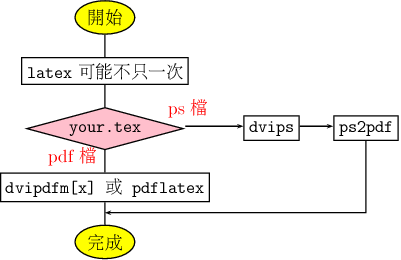
\includegraphics{latex-flow}
\end{center}

\section{\LaTeX\ ���S���M�βŸ�}
�b \TeX/\LaTeX\ ���@�ɡA��l��Z���O�¤�r�ɡA����@�ؽs�边���i�H���}�ӽs��B�[�ݡC�ӱƪ����O�q�`�O�Ѥϱ׽u�]\textbackslash, backslash�^\index{�ϱ׽u}\index{backslash}�Ҷ}�Y�Ӥ޾ɡC����\index{����}�h�O�Ѧʤ����]\texttt{\%}�^�Ӥ޾ɡC�Ҧp�A�H�s�边�s��U�C��r�G

\begin{quote}
\begin{verbatim}
This is my first \LaTeX\ typesetting example.
\end{verbatim}
\end{quote}

�sĶ��|�ܦ��H�U�����G�G

\begin{quote}
This is my first \LaTeX\ typesetting example.
\end{quote}

�䤤�� \verb|\LaTeX| �N�O \LaTeX\ ���@�ӫ��O�A�|��� \LaTeX\ �o�ӯS�����ϥܡC

�ѩ�A����a���y�t�A�q�`�r���B�Ÿ����̤j�e�q�u�� 256 �ӡ]$2^8$�^�A�]���A�\�h�{�����Ÿ��������ӷ���������O�A�~��ŦX�ƪ����h�ˤƻݨD�C�H�U���Ÿ��A��IJ \TeX/\LaTeX\ ���B�͡A�i�ೣ�o�ɮɯd�N�A���n���g�B�z�N�����g�i��Z���Y�h�F�C

�q�`�A�s�边���y�k�C��\index{�y�k�C��}�|���U�P�_�y�k�O�_���T�A�����O���৹���L�ʡA�����٬O�|�|���A�o�ɧO�ѤF�d�ݤ@�U {\tt *.log} �ɮסA�Ҧp�G�sĶ {\tt your.tex} �ɪ��ܡA�L�� log �ɴN�O {\tt your.log}�C

\begin{quote}
\begin{tabular}{llll}
�Ÿ� & �@�� & ��Z�W�ϥ� & \LaTeX\ �����N���O \\
\hline
\textbackslash & �U�ƪ��R�O & \verb|$\backslash$| & \verb|\textbackslash|\\
\%             & ����       & \verb|\%|           & NA \\
\#             & �w�q����   & \verb|\#|           & NA \\
\~{}           & ���ͤ@�Ӫť�   & \verb|\~{}|     & \verb|\textasciitilde| \\
\$             & �i�J�]���}�^�ƾǼҦ� & \verb|\$| & \verb|\textdollar| \\
\_{}           & �ƾǼҦ������ͤU�Цr & \verb|\_{}| & \verb|\textunderscore| \\
\^{}           & �ƾǼҦ������ͤW�Цr & \verb|\^{}| & \verb|\textasciicircum| \\
\{     & �ХܩR�O���@�νd��   & \verb|\{| & \verb|\textbraceleft|\\
\}     & �ХܩR�O���@�νd��   & \verb|\}| & \verb|\textbraceright|\\
\textless      & �ƾǼҦ������p��Ÿ� & \verb|$<$| & \verb|\textless| \\
\textgreater & �ƾǼҦ������j��Ÿ�   & \verb|$>$| & \verb|\textgreater| \\
\textbar     & OT1 �s�X�A�ƾǼҦ����~�ॿ�T��� & \verb+$|$+ & \verb|\textbar| \\
\&           & ���椤�����j�Ÿ�   & \verb|\&| & NA
\end{tabular}
\end{quote}

\section{\LaTeX\ �ƪ��W���@�dzW�d�κD��}
\label{sec:convention}\index{�W�d}\index{�D��}

���F�W���ҽͨ쪺�S���Ÿ��~�A�]���@�dzW�d�κD�ҭn���u�A���ǬO����w�ʪ��W�w�A���ǫh�u�O�D�ҡA�i�ण�P����a�B�y���|�����P���D�ҡA�Ȯɥ���L�����O \LaTeX\ ���C���W�h\index{�C���W�h}�N���F�C

\subsection{�r���������N�y}
\label{subsec:baseline}

�n�ͱƪ��W���W�d�B�D�ҫe�A�ڭ̱o���{�Ѥ@�U�r�����@�dzN�y�A�H�K����峹������ɦ��ӷ����C�q�`�ڭ̨C�Ӧr���O�m���@�Ӱ��Q����ؤ��A�٬� em-square\index{em-square}�A�P�@�Ӧr�����P�@���I�ơA�C�@�� em-square �j�p���O�ۦP���A��ڤW���r�]glyph\index{glyph}�^�n�m��b�o�� em-square �������m�A�o�O�r���]�p�̪��[�I�A�ҥH�A�P���I�ƪ����P�r���A�L���r���j�p���@�w�|�@�ˡA�]���ڭ̬O�ϥ� em-square ���j�p�b������A�ӫD��ڪ� glyph�C

�b�峹���ƦC���ɭԡA�h�O�N glyph �m��@�ӥH���Q�Ѧ��I�]reference point�^\index{���Q�Ѧ��I}\index{reference point}����Ǫ��@�Ӱ��Q�u�W�A�٬���u�]baseline\index{��u}\index{baseline}�^�A�j�g�r�����F Q �H�~�A�L�̪��������O�m���u�W���C���p�g�r���h���@�w��n�y���b��u�W�A���Ǧr�����e�i��W�X��u�H�U�A�Ҧp y�Bj ���r���C����r���b�峹�����m���m�A�ڭ̨Ӭݬݤ@�Ӽ����ϡG\footnote{��ڦr���]�p�W���U�����M���W���ε��c�A���M���|�O�o��²���A�o�̪������ϡA�u�O�Ȯ����r���@��m�񦳭Ӳʲ��������C}

% looks ugly, but l2h cannot handle this MP file be transparent png.
\begin{center}
\latexhtml{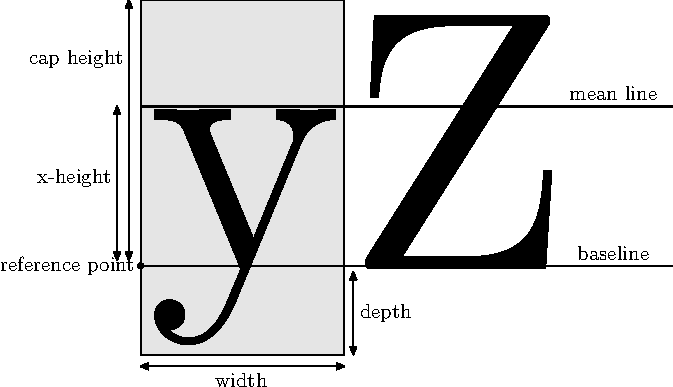
\includegraphics{baseline.1}}{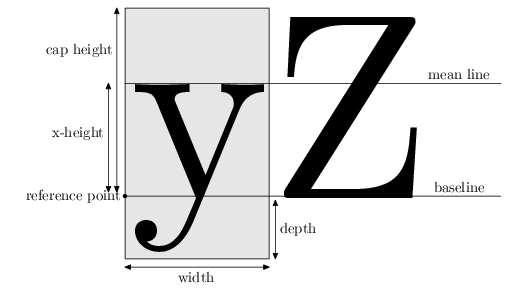
\includegraphics{baseline}}
\end{center}

�o�ӶW�X��u�H�U�����סA�ڭ̺٤����`�ס]depth\index{�`��}\index{depth}�^�A�H�W���N�٬��r���]height\index{�r��}\index{height}�^�A���M�j�p�g�����P�S�����j�g�r�����r���]cap height\index{cap height}�^�Τp�g�r�� x ���r���]x-height\index{x-height}�^�A�ѩ�o�ӨҤl�̬O�զX�r\index{�զX�r}�A�ҥH�C�Ӧr���e�ס]width\index{�e��}\index{width}�^���@�w�|�@�ˡA�����r���r�ڪ��h�O���e���r���C�r���[�W�`�סA�ڭ̴N�٤��� totalheight\index{totalheight}�A�j���������p�A�ȶȻ� height �ɬO���]�A depth ���A�ӥB�q�`�����O cap height�C

mean line\index{mean line} �b�@�����֥Ψ�A�q�`�O�r���]�p\index{�r���]�p}�ɤ~�|�Ψ�A�L�O���p�g�r���h���W����X�������ҳs�����@�Ӱ�ǽu�A�o�� mean line �� baseline ���Z���A�@��N�٬� x-height�A���M�N�O�p�g�r�� x �����סA�]���ڭ̷|���@�Ӫ��׳��A�٬� ex�A�����N�O�o�� x-height�C

����r���ܤ���S���A�L�O�H em-square �������I�Ӹm�� glyph ���A�b���^��V�X�ɡA����r�ä��O��n�y�����u�W���A�|�W�X��u�U�@�I�I�A�ܩ�|�W�X�h�֡A�h�M�r�����]�p�����A�C�ئr�������i��|���P�C�o�]�O���D�ƪ��W���@�P�ʡA�r���i�ೣ�ݭn�ɶq�ϥΦP�@�M���U�ئr������]�A�_�h�N�o�g�L�L�աA�~��Ͼ�Ӧr�����{�W���o��դ@�P�C

�o�DZM���N�y�A���ᴣ��@�ǫ��O���Ѽƪ��y�z�ɳ��|�ϥΨ�A�]�������x�@�U�A�Ҧp�G�r�������\index{�r������}�A��ڪ��N�O�H�Ѧ��I�]reference point�^���ǡA�u�����X���b�ߨӱ��઺�A�Ӥ@��һ�����Z\index{��Z}�A�����O�W�U�� baseline ���Z���C

\subsection{�@��ʪ��C���W�h}
\label{gen:gamerules}\index{�C���W�h}

\begin{enumerate}
\item \LaTeX\ �����O���O�j�p�g���O���A�� \verb|\| �}�Y�A�ᱵ�Ѧr���զ����r��γ�@���D�r���r���C�䤤�� \verb|[ ]| ���A���A�����O��ܩʰѼ�\index{��ܩʰѼ�}�A�i�H�ٲ��A�� \verb|{ }| �j�A���A�����O����ٲ����ѼơA���M�A\LaTeX\ �����O���@�w�|���ѼơA�����j�������|���ѼơA�u���L��L���ٲ��ϥιw�]�Ƚ}�F�C

\item \LaTeX\ ��Z���A�Ť@�ӭ^��ťթM�Ŧh�ӭ^��ťժ��@�άO�@�ˡA\LaTeX\ �|�{�@�@�ӭ^��ťաC

\item ���`�ڭ̽s��¤�r�ɡA���� \textsf{Enter} ��A�N�N������A����ڱƪ��X�ӡA�@�檺�e�׬O���ӱƪ��������]�w�A�]�N�O���A�A�b��Z���� \textsf{Enter}�A���N���ƪ���N�O�q�o���_��\index{�_��}�A\LaTeX\ �|�̤@���������e�׸g�L����p���۰ʸɦ��@����A���_��A�ӥB�|�b�����۰ʸɨ��@�ӪťաC�o�b�^��ܦ۵M�A�٬��r�]word�^���ť�\index{�r���ť�}�A������h���@�ˡA�b�s�边���s�褤��A�H�N�� \textsf{Enter} �����G�A�|�y���峹�������嶡�X�{�ťաC�o�|�b���夤�A�����ɾ��A���X�ѨM����k�C

\item �s�边���A�h���X�� \textsf{Enter} �N�h�ťX�X��A���b \LaTeX\ ��Z�̡A�h�Ӫťզ�\index{�ťզ�}�A�M�@�Ӫťզ�O�@�˪��@�ΡA\LaTeX\ �|��L�{�@�O�@�Ӫťզ�C�ӳo�Ӫťզ�A\LaTeX\ �P�ɤ]�|�{�@�O�s�q�����}�l�A�ҥH \LaTeX\ �O�H�ťզ�Ӥ��j�U�Ӭq���C

\item \LaTeX\ �w�]�C�ӳ��`���Ĥ@�Ӭq�����Ĥ@��O�����Y�]noindent\index{�����Y}\index{noindent}�^�A�q�ĤG�Ӭq���}�l�~�|���Y�]indent\index{���Y}\index{indent}�^�C���M�A�o�O�i�H��諸�A����|�A���ΡC

\item \LaTeX\ �����O�A�O�q�ϱ׽u\index{�ϱ׽u}��Ĥ@�Ӧr���}�l�A��Ĥ@�ӫD�r���Ÿ�����]�]�A�ťաB���I�Ÿ��μƦr�^�C�]���G

\begin{quote}
\begin{verbatim}
This is my first \LaTeX typesetting example.
\end{verbatim}
\end{quote}

�o�˪��ܡA��ڵ��G�A�]�� \verb|\LaTeX| �᪺�ťլO�ݩ���O���@�����A�ťձN���|�Q�����A�o�˷|�L���G

\begin{quote}
This is my first \LaTeX typesetting example.
\end{quote}

�o�ص��G�A\LaTeX\ �M typesetting �s�b�@�_�F�C�n�קK���ܡA�N�n���w���O���@�νd��A�Ҧp�H�U���j�A���C�δN�u���[�ӪťաA�Ҧp \verb|\ |�A\LaTeX\ �I�� \verb|\| �N�|�Φ����㪺���O�A��᪺�ťմN�|�Q�u���������ťդF�G

\begin{quote}
\begin{verbatim}
This is my first {\LaTeX} typesetting example.
This is my first \LaTeX{} typesetting example.
This is my first \LaTeX\ typesetting example.
\end{verbatim}
\end{quote}

�ҥH�A���`�L�X�����ӬO�G

\begin{quote}
This is my first \LaTeX\ typesetting example.
\end{quote}

\item ���ѲŸ��]{\tt \%}�^\index{���ѲŸ�}\index{%@\verb=%=}�A�i�H��b�@�檺����a��A{\tt \%} �᪺��r�|�Q \LaTeX\ �����C�ҥH�A�p�G�O��b�@�檺�̧��ݡA���� \LaTeX\ �|�۰ʴ��J���r���ťդ]�N�|�Q�����C�Ҧp�G

\begin{quote}
\begin{verbatim}
This is my fisrt \LaTeX\ document. Give \LaTeX\ a%
try.
\end{verbatim}
\end{quote}

�o�ˤ@�ӡA�ƪ��X�ӷ|�ܦ��G

\begin{quote}
This is my fisrt \LaTeX\ document. Give \LaTeX\ a%
try.
\end{quote}

a �M try �s�b�@�_�F�I���`���ӬO�G

\begin{quote}
This is my fisrt \LaTeX\ document. Give \LaTeX\ a try.
\end{quote}

���o�ӯS�ʡA�ڭ̥i�H���Φb����A�]�N�O���b�s�边\index{�s�边}���A����峹�� \textsf{Enter} �䴫��ɡA���ݥ[�� {\tt \%}�A�o�ˤ@�� \LaTeX\ �N���|���J�^��r���ťաA����r�N�i�H�s�������S���ťժ��@���F�A�_�h \LaTeX\ �b��g��Z�_�y\index{�_�y}�ɡA�|�۰ʦb�촫��B��J�@�ӭ^��ťաA�]���A��l�� \TeX/\LaTeX\ �O�{���o���媺�C

\item ���^��V�X���ɭԡA�q�`�A�^��r�e�᳣�|�d�ӪťաA�H�K�M����Ϲj�}�ӡA�u�O�o�Ӫťխn�h�j�A�o�N�S���T�w���D�ҡA�q�`�d�ӭ^��ťդ]�O�i�H�A�n���s���ܡA���ͨ줤��ƪ�����ij�D�ɦA�ӰQ�סA�ثe�N�i���ߺD�A�^���r�e��d�ӭ^��ťաC
\end{enumerate}


\subsection{�w����I�Ÿ����C���W�h}

\begin{enumerate}
\item ���^�媺�޸�\index{�޸�}���@�ˡA�o�̽ЯS�O�`�N�A�\�h�H�`�`�d���C���B�^��޸����޳������n�����k�C�^�媺�ܡA���䪺�޸��O grave accent�A�O��L���W�� {\sf Esc} �� {\sf F1} �U�観�i�θ������@����F�k�䪺�O apostrophe\index{apostrophe}�A�]�N�O��L���� {\sf Enter} ��j����������C���޸������άO��J�⦸������޸�\index{����޸�}�Ψ⦸���k��޸�\index{�k��޸�}�A�Ӥ��O�� \verb|"| �o�Ӥ@����������I�� ditto marks\index{ditto marks}�C�ҥH�A��ڤW�b��J��Z�ɬO�G

\begin{quote}
\begin{verbatim}
Please press an `Esc' key.
Please press an 'Esc' key. �o�O���~�ܽd�I
``This sentence.''
"This sentence." �o�O���~�ܽd�I
\end{verbatim}
\end{quote}

�ƪ��X�Ӫ����άO�G

%begin{latexonly}
\begin{quote}
Please press an `Esc' key.\\
Please press an 'Esc' key. �o�O���~�ܽd�I\\
``This sentence.''\\
"This sentence." �o�O���~�ܽd�I
\end{quote}
%end{latexonly}

\begin{htmlonly}
\begin{quote}
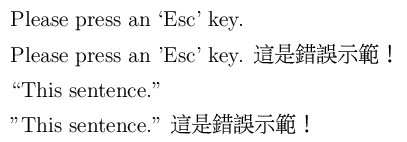
\includegraphics{quotation}
\end{quote}
\end{htmlonly}


���媺�ܡA�ڭ̬O�ϥΤ�����Ϊ��u�B�v�Ρy�B�z�A�b����j���h�w��ΩM�^��ۦP�Ϊ������βŸ��A���o�b���媽�Ʈɷ|�X���D�A�]���A���媺��B���޸��٬O�o�����ڭ̥ثe�ϥΪ��C

\item \LaTeX\ �|�b�^��峹���@�ӥy�l�����M�t�@�ӥy�l�}�l�������A�۰ʽվ㦨���j�@�I���ťաA�o�i�H�W�[�峹����Ū�ʡC�ҿפ@�ӥy�l�����A�Ҧp�G�y�I�].�^�B�ݸ��]?�^�B��ĸ��]!�^�Ϋ_���]:�^�A�o���M�O���^�媺�b�μ��I�Ÿ��A���O���媺���μ��I�Ÿ��C�A�i�H�`�N�@�U�W�����|���Ҥl�A�b document.\ �M Give �������ťշ|�y�L�j���L�^���r�����ťաC

�{�b�����D�O�A�p�G�o�Ǽ��I�Ÿ��᭱���O�t�@�ӥy�l���}�l���ɭԡA\LaTeX\ �L�k�h�P�_�o�ر��ΡA�o�ɱo�ѧڭ̦ۤv�ۦ�P�_�B�B�z�F�C�Ҧp�^���Y�g�r�G

\begin{quote}
\begin{verbatim}
I am Mr. Edward G.J. Lee, G.J. is a abbreviation of my name.
I am Mr.~Edward G.J. Lee, G.J. is a abbreviation of my name.
I am Mr.\ Edward G.J. Lee, G.J. is a abbreviation of my name.
\end{verbatim}
\end{quote}

�䤤 \verb|Mr.\ Edward| ���g�k�A�M \verb|Mr.~Edward| �X�G�O�@�˪��A���O�j�����J�@�Ӥ���p�����`��r���ť�\index{��r���ť�}�A�t�O�b���̤]�t�~���ܤ��i�H�q�o�̴���A�q�`�Φb�H�W���ɭԡA���L�̤��P���_�A�@��b�H�W���ƪ��A�]�A�L���Y�ΡB¾�١A�O�����_�����Ӥ��}���C�ӥB��Ӥ�y�������ܡA�H��̸�����A�~���|�]���_��Q������b�A�o�� {\tt ~} �Ÿ��]�]���b \TeX\ ���M���W���A�N�٬� tie\index{tie}�A��L�̸j�����N��C�ƪ��X�Ӫ��ɭԷ|�ܦ��G

%begin{latexonly}
\begin{quote}
I am Mr. Edward G.J. Lee, G.J. is an abbreviation of my name.\\
I am Mr.\ Edward G.J. Lee, G.J. is an abbreviation of my name.
\end{quote}
%end{latexonly}

\begin{htmlonly}
\begin{quote}
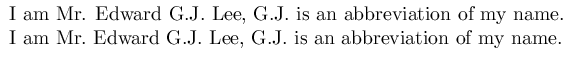
\includegraphics{abbreviation}
\end{quote}
\end{htmlonly}

�Щ�j�h�J�Ӥ���@�U���G�N���D�F�C�ĤG�檺�~�O���T���AMr.\ �M Edward �������ťլO���`��r���ťաA��Ĥ@�檺�y�l�����ťխn�p�@�I�I�C��L���ϥΨ��Y�g�r�����X�A�Ҧp�G`Dr.'�B`etc.'�B`e.g.'�B`i.e.'�B`vs.'�B`Fig.'�B`cf.'�B`Mrs.'�A�o�dz����O�N���y�l�����A�ҥH�A�n���J�@�ӥ��`�ťաC

�� G.J. �᭱������S�����J���`�ťաH���O�]���AJ �O�j�g���A�o�� \LaTeX\ ���|�h�~�{���O�y�l�����A�q�`�y�l�����ɪ��y�I�e�����Ӧr���O�p�g���CWell�A���S��ı�o���I�D�z�H:-)

�����A�Ʊ��٨S�������IKnuth �б¥X�F�@�D���D�A�p�G�y�l�������O `Please see Appendix A.' �᭱�S�ٱ����t�@�ӥy�l�C�o�ɫ���H�ѩ�A���|�{���O�y�l�����A�]���|���J���`�ťաA���o���O�y�l�����r�I�мȮɥ��O�o�A�ϥ� \verb|...Appendix A\null.|�A�� \verb|...Appendix A\@.|�C�o�ӻ��Ӧ��I�ܪ��A�����|�A�ӱ��Q�A�аO�o `\verb|\null|' �M�y�I���O�S���ťժ��C�Ҧp�G

\begin{quote}
\begin{verbatim}
Please see Appendix A. We will be there soon.
Please see Appendix A\null. We will be there soon.
\end{verbatim}
\end{quote}

�ƪ��X�Ӫ����G�N�|�O�]�t��������A�Фp�ߤ���^�G

%begin{latexonly}
\begin{quote}
Please see Appendix A. We will be there soon.\\
Please see Appendix A\null. We will be there soon.
\end{quote}
%end{latexonly}

\begin{htmlonly}
\begin{quote}
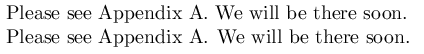
\includegraphics{abbreviation2}
\end{quote}
\end{htmlonly}

�p�G�A�A�{�b�\Ū���O HTML\index{HTML} �榡���A���ǨҤl�p�G�L�k������ܥX�ӡA�Ч�\�� PDF �����C�ӥB�A�p�G�A�s�@ PDF �榡�ɡA�r���S�����O�]���媺�^�Ʀr�O�O�J Computer Modern Type1 �r���^�A�t���i��N�|�󤣩���C�i�յۨϥ� {\sf gv/gsview}\index{gv@\textsf{gs}}\index{gview@\textsf{gview}} �h�\���A�M��վ㦨 Landscape\index{Landscape}�A��y�l�����Ԩ���t���a��h�N�ݱo�X�ӤF�C�o�b�y�l�h���ɭԡA�o�Ӫťդ]�ëD�T�w�j�p���A\LaTeX\ �|���峹���c���ݭn���ӷL���վ�C

\item �R�`��\index{�R�`��}����^�]�O���P�A�^��O�T�I�A�p�G�I��y�I���ܡA�h�O�|�I�C���媺�ܬO���I�A�I�줤��y�I�ܮe���N���o�M���C���O�^��o�ӤT�I�A���O�N���ӤT�ӥy�I�F�ơA�o�˪��I�ӱK���A�i�H�ϥ� \verb|\ldots| �� \verb|\dots| ���O�A�Ҧp�G

\begin{quote}
\begin{verbatim}
I'm not a good man ..., but a good husband .... ���~�ܽd�I
I'm not a good \ldots\ man \ldots, but a good husband \ldots.
I'm not a good \dots\ man \dots, but a good husband \dots.
\end{verbatim}
\end{quote}

�ƪ��X���ӵ��G�O�G

%begin{latexonly}
\begin{quote}
I'm not a good ... man ..., but a good husband .... ���~�ܽd�I\\
I'm not a good \ldots\ man \ldots, but a good husband \ldots.\\
I'm not a good \dots\ man \dots, but a good husband \ldots.
\end{quote}
%end{latexonly}

\begin{htmlonly}
\begin{quote}
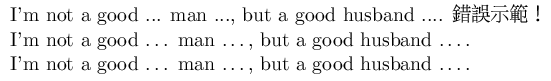
\includegraphics{dots}
\end{quote}
\end{htmlonly}

���媺�R�`���O�Ѩ�ӥ��Ϊ��T�I�Ҳզ����I���A�Y�G\chdots{}�A�N�O�ڭ� Big-5 �X�� {\tt 0xa14b}�]{\tt U+2026}�^�A���ѩ� Unicode\index{Unicode} �|���@�� MIDLINE HORIZONTAL ELLIPSIS({\tt U+22EF})�A�]���A���dzn��b��Ū�W���i��|���@�ˡA�]���ڭ̪��r���A�j�����b�s�@���I�Ÿ��ɬO�m�b�������a��A��������j���O�m��b��u���a��A�� Unicode �x��ĥΪ��˥��r���A��n�O����j�����t�өҴ��ѡA�o�ˤ@�Ӧ��dzn��u�@�̴N�{���ڭ̪��R�`�����ӬO {\tt U+22EF} �F�A�ܤ������A�ڭ̪� Big-5\index{Big-5} �X�èS���۹������r�X�C

\item �}�鸹\index{�}�鸹}�C�b�^��A�۷���}�鸹���i�঳�T�ءG
  \begin{itemize}
    \item hyphen\index{hyphen}\\
�o�O�̵u�� dash\index{dash}�A�q�`�N�O��J \verb|-| �N��F�A�Ҧp \verb|father-in-low|�A�o�˷|���{�� fater-in-low�C
    \item en-dash\index{en-dash}\\
�o�O�̱`�Ϊ��}�鸹�A�O��J��� hyphen�C�Ҧp \verb|1991--2003 �~|�A�o�|���{�� 1991--2003 �~�C
    \item em-dash\index{em-dash}\\
�o�O�̪��� dash�A�ѤT�ӳs�� hyphen �զ��A���ӬO�̬۪��ڭ̤���һ����}�鸹�C�Ҧp \verb|I am---a good man.| �|���{�� I am---a good man.�C�ܩ�o�ӤT�ӳs�� hyphen �e��O�_�n�d�ťաA�����H�ϥΡA�èS���w�ʪ��D�ҡA�����F�M���媺�}�鸹�t�X�]����}�鸹�e��A�q�`���d�ťա^�A�ӤH�q�`�O���d�ťժ��C
    \item �u�����\\
�o�������O�}�鸹�A�ӬO��ڪ���έt���A�o�n�i�J�ƾǼҦ��A�Ҧp�G�t���A�n�g�� \verb|$-5$|�A�M����{�X�ӬO $-5$�C�o�]�`�`�|���H�d���A���ઽ����J�@�몺�t��������ӥR�ơA�o�O�]�� \TeX/\LaTeX\ ���ƾǦ��l���Φr�M���j�B�z�A�M�@�뤺�夣�P�����Y�C
    \item ���媺�}�鸹\\
���媺�}�鸹�O����Ӥ���r��m�����@��u�A���שM�R�`���ۦP�C�b���u��m���A�w�q�W�O����ءAen-dash �O {\tt Big-5 0xa156}�Aem-dash �O {\tt Big-5 0xa158}�C���ѩ󤤤�r���Z�����D�A���i�ॴ�X�Ӫ��}�鸹�����|���@�I�ť�\footnote{�o�O�i�H�վ㪺�A�]�N�O�h����Ӿ�u�������r���Z�A�o�˴N���|���ͤp�ťդF�A����R�`���]���P�˪����ΡA�ڭ̷|�b�L�ժ������A�ӰQ�סC}�A�Ҧp�X�X���媺 em-dash�A�o�O�V�V���媺 en-dash�C�b�פ夤�A�}�鸹�q�`�i�H�ϥΤp�A���Ϋ_���N���C
    \item ���媺�p�W���ήѦW��\\
���媺�p�W��\index{�p�W��}�A�i�H�Щ��H�W�B�a�W�A�p\underline{�]�h�P}�F�ѦW��\index{�ѦW��}�]�p�W�������u�����i���Ϊ��^�A�i�H�Φb�ѦW�A�o�DzŸ��`�y���ƪ��W���x�Z�A�`�ϥ� �m �n�Ө��N�ѦW���A�p�W���h�L��L���N��k�C�b�@�몺�۵M�����ά�ǽפ�W�q�`���ϥγo���¦����p�W���ήѦW���C
\end{itemize}

\item ���Y�I\index{���Y�I}\\
�o�i�O�ƪ������n�\��C�^�媺�q�`�S�����D�A\LaTeX\ �|�۰��׶}�B�z�A����N���@�w�F�A\LaTeX\ �i���{�Ѥ���A���q�`��������{���ήM��A�h�h�ֳ֤��|�B�z�A�u���L�A���ɭ԰����i��|�~�P�C����A�쩳����O���Y�I�H���U�C�Ӫ��A�j�a�N���դF�A�ڦC���媺�A�^�媺�N���C�X�ӤF�A�]�� \LaTeX\ �|�۰ʳB�z�A�����ڭ̾�ߡC

\begin{quote}
\begin{tabular}{ll}
���I�Ÿ� & �m��B\\
\hline
�A�C�F�B:�v�^�n�I�H & ����m��歺\\
�u�]�m              & ����m����\\
�}�鸹�ΧR�`��      & �m�󭺧��ҥi\\
\end{tabular}
\end{quote}

²�檺���A���F�}�鸹�ΧR�`���A�S���}�f���A����m��̶}�Y�A�}�f�V�k���A����m��̥k�A�}�f�V�����A����m��̥��C�q�`���|�B�z�n�A���սZ���ɭԭn�`�N�@�U�~�P���a��C
\end{enumerate}

\section{\LaTeX\ ����Z���c}
\label{sec:struct}\index{��Z���c}

\subsection{���ҡ]environment�^\index{����}\index{environment}}

�W�@�`�ҽͪ����O���O�A���M�]�i�H�Ѥj�A��\index{�j�A��}�өw�@�νd��A���p�G�O�@��q�A�ƦܬO�@��g�峹���n�@�ήɡA�����O�i��N���ܾA�X�F�A�]���A\LaTeX\ �]���@�إ������c�A�٬����ҡ]environment�^�A�D�n�O���@�νd����X�j�ܸ��j���d��C

�Ҧ������ҡA���O�_�� \verb|\begin{���ҦW��}|�A��� \verb|\end{���ҦW��}|�A�o��ӫ��O��������Z���|�Q�@�ΡA�ӥB�A���Ҥ����٥i�H�M�Ψ�L���P�����ҡC

\LaTeX\ ��Z������A���N�O�]�b�@�� \verb|\begin{document}| �M \verb|\end{document}| �o�� document ���ҷ����C

\subsection{��²�檺 \LaTeX\ ����Z���c}

�H�U�N�O�Ҧ� \LaTeX\ ���ݨ�ƪ���Z�j���c�G

\begin{quote}
\begin{verbatim}
\documentclass{article}

  �o�̬O preamble ��

\begin{document}

  �o�̬O�����

\end{document}
\end{verbatim}
\end{quote}

\verb|\documentclass{article}|�A�o�O�b�i�D \LaTeX\ �ϥέ��@�����O�A�ڭ̥ثe�ϥΪ��O {\tt article} ���O\index{���O}\index{article}�A�������O�|�b�� \ref{ch:class} ���Q�סCpreamble\index{preamble} �ϡA�h�O�U�@�Ƿ|�v�T��Ӥ�Z�����O�A�ΤޥΥ����M�󪺦a��A���M�A�������ޥΥ����A�]���ϥμv�T���媺���O���ܡApreamble �ϴN�O�ťաA���g����F��C����ϡA�N�O�ڭ̹�ڤW�g�峹���a��C

�{�b�]�i�H��e�����|���Ҥl�A��J����ϸ��Y�Apreamble �ϪťըS���Y�A�M��s�ɡA�յ۽sĶ�ݬݡG

\begin{quote}
\begin{verbatim}
latex example.tex
dvips example.dvi      => ���� ps �榡 example.ps
dvipdfm[x] example.dvi => ���� pdf �榡
pdflatex example.tex   => ������ .tex ���� .pdf
\end{verbatim}
\end{quote}

�u������Ҹѻ��A�|�b�U�@���Ӷi��A�ҥH�A�o�̼Ȯɤ��|���Ц��������ҥi�H�ϥΡA�����ݬݨS�����Y�C�ѩ��٨S�ͨ줤�媺���D�A�]���p�G�A�Q�ոլݡA���Ȯɥ��ϥέ^��A�D�z���O�۳q���C

\subsection{preamble �ϥi�H��Ǥ���H}
\label{subsec:preamble}

�o�̥i�H�ޥΥ����A�ӥB�|�v�T��g��Z�����O�A�Ҧp�@�Ǩƥ��w�q�n�����O�A�Q�b��g��Z���ϥΡA�N�i�H�m��b preamble �ϡC

\subsubsection{�������ޥ�}
\label{subsubsec:package}

����D�n�O�з� \LaTeX�A���e���w����A�|���ǥ����M�󤣱o���n�ޥΡA���U�N�ӻ����p��ޥήM��C�o�ǮM�󳣬O�@�� \TeX\ �t�γ��|���W���C

���O�����ҭn�p��}�Y�����йL�F�A�{�b�ӬݬݤޥΥ����n���}�Y�C

\begin{quote}
\begin{verbatim}
\documentclass{article}
\usepackage{color}
\begin{document}
\textcolor{blue}{This is blue color.}
\end{document}
\end{verbatim}
\end{quote}

�sĶ�@�U�A�ݬݵ��G�O����H�o�̨ϥΪ��N�O \textsf{color} package\index{color@\textsf{color}}�A���Y�O�� \TeX/\LaTeX\ macro �Ҽg���@�ӥ����M��C�@��²�檺�ڭ̴N�٬������]macro�^\index{����}\index{macro}�A�����@�I���N�٬������M��]package�^\index{�����M��}\index{package}�A���A���Y���O�@�˪��A�u���L�j�p�Φ��S����z���@�Өt�Ϊ��t�O�C

\LaTeX\ ���Y������{�����M��i�H�ϥΡA�C�Ӵ��G�� \TeX\ �t�ΩҦ������i�ೣ�|���Ҥ��P�C�j���S���H�i�H��q�Ҧ��{�s�� \LaTeX\ �����M��A�]����b�O�Ӧh�F�A���L�A����j�����|����`�Ϊ������M��C�ԲӪ������M�󪺺غءA�|�b�� \ref{ch:package} ���ӻ����C

\subsubsection{�v�T��g��Z�����O}

�|�v�T��g��Z�����O�A�q�`�]�O��b preamble �ϡA�Ҧp�G

\begin{quote}
\begin{verbatim}
\linespread{1.36}
\parindent=0pt
\end{verbatim}
\end{quote}

\verb|\linespread| �O�b����W�U�檺��Z�A�o�̴N�O�N��Z�ܦ���Ӫ� 1.36 ���C�ܩ󤰻�O��Z�O�H�N�O�o�@�檺��u�]baseline�^��U�@�檺��u���Z���A�q�`�^��峹�����h�վ�L����Z�A������o�A���[�j��Z�H�Q�\Ū�C

\verb|\parindent| �O�վ�q�����Y���{�סA�o�̽վ㦨 0�A�]�N�O���U�q���������Y���N��A�]�i�H�վ㦨��L���ȡA\LaTeX\ �N�|�̳o�ӭȥh���Y�C���M�A���h�]�w���ܡA\LaTeX\ �N�|�̥L���w�]�ȥh���Y�C


\subsection{���`���c\index{���`���c}}
\label{subsec:chapstruc}

����Ϸ��M�O�ڭ̼g�峹���D�n�a��A�Τ@�ǷL��\index{�L��}�C�b \LaTeX\ ����Z���Y�A���`���D���Φ����O�ѦP�˪����O�ӱ���A�o�˦��@�Ӧn�B�A�{�ɴ��J���`���D�Ψ䤺��ɡA�ڭ̤����h�z�|���D�s���Υؿ������D�A�]�����h�z�|�n�Τ���r���B�Φr���j�p�n�h�j�A\LaTeX\ �|�۰ʭp��B�z�A�r���j�p�]�|�M����ϥΪ��r���j�p���۰t�X�վ�A�ϥΪ̴N�M�ߦb����c��B�g�@�Y�i�C�H�U�ѦC�����A�Ѿ�ӳ��`���c�G

\begin{quote}
\begin{tabular}{lll}
�`�׼и� & ���O & �@�ΤΪ`�N�ƶ�\\
\hline
$-1$ & \verb|\part{}|          & �o�O�̤j�����c�A�ڭ̤���q�`�٬��u���v�C \\
0    & \verb|\chapter{}|       & ���C�b article ���O���Y�S�����C\\
1    & \verb|\section{}|       & �`�C\\
2    & \verb|\subsection{}|    & �p�`�C\\
3    & \verb|\subsubsection{}| & ���p�`�C\\
4    & \verb|\paragraph{}|     & �q���C\\
5    & \verb|\subparagraph{}|  & �p�q���C\\
\end{tabular}
\end{quote}

���`���D\index{���`���D}�����e�N�O�����g�J���O���j�A�����Y�N�i�H�F�A\LaTeX\ �b�ƪ��ɷ|�۰ʨϥβ���B�[�J���`�s��\index{���`�s��}�ίǤJ�ؿ�\index{�ؿ�}���Y�C

�ܩ�Ĥ@�檺�`�׼и��]secnumdepth�^\index{�`�׼и�}\index{secnumdepth}�A{\tt book/report}\index{book@\texttt{book}}\index{report@\texttt{report}} ���O���`�׼и��O 2�A{\tt article} ���O 3�C�o�O����N��O�H�N�O�� {\tt book/report} ���O����Z�A�b \verb|\subsection{}| �H��]{\tt subsection} �������|�s���^�A���`�N���A�s���F�F�P�˪��A�b {\tt article} ���O����Z�A�b \verb|\subsubsection{}| �H��N���s���F�C�����M�|�W�ߥX�@��W��Ӫ��ܳo�ӬO���D�C���s���F�����`���e�A���M�]�N���ǤJ�ؿ����Y�F�C�o���M�O�i�H��諸�A�u�n��� \LaTeX\ �� {\tt secnumdepth} �o���ܼƪ��ȴN�i�H�F�A�o�ө���|���Φp���� \LaTeX\ ���w�]�ȡC���o�g�峹�A�b preamble �ϴN���@�ӳ]�w�G

\begin{quote}
\begin{verbatim}
% let the depth of report to subsubsection
\setcounter{secnumdepth}{3}
\end{verbatim}
\end{quote}

�ҥH�A�o�g�峹���M�ϥΪ��O {\tt report} ���O�A���O���`���`�׼и��O�Цb 3�A�]�N�O���|�s���� {\tt subsubsection} ����A���o���M�O�S���s�J�ؿ������C 

�U�@���N���ڭ̶}�l��ڰʤ�a�I��\chdots{}�A����{�b���S�����㤶�Ы��O�O�H���ګ��|���D��������O�i�H�ϥΡH�o�O�]�� \LaTeX\ �����O�ܦh�A�������Ъ��ܡA�@�譱�O�����A�G�譱�]���e���A�ѥL����ڧ@�ΡA�ҥH�A�ڭ̱N�|�b�U���|�Үɬﴡ�b���Y�����A���o����󱵪���n�ɡA�A�Ӿ�z�ӫ��O�t�d���A�o�˥H��d���O�N�ܤ�K�F�A�����h���O�A�u�n���D���ӳo�˥\�઺���O�N���F�C


% ``�j�a�Ӿ� LaTeX'' LaTeX ��Z start.tex
% Copyright (c) 2004  Edward G.J. Lee <edt1023@info.sayya.org>
%
% �b���H�� GNU Free Documentation License 1.2 �ΥH�᪺�����W�d���U�A
% ���\�����B���G�έק�C���쪩�v�B���v�n�����o�����C
%
% �����G�����A�t�� fdl.tex�A���e�� GNU FDL ���W�d���C�p�G�򥢡A�i��
% http://www.gnu.org ���o�A�μg�H�ܦۥѳn�����|(Free Software Fundation)
% �����C
% 9 Temple Place - Suite 330, Boston, MA 02111-1307, USA.
%
% $Id: start.tex,v 1.38 2004/03/07 12:29:47 edt1023 Exp $
%
\chapter{��ڤW�ƪ����ݬ�}
\label{ch:start}

�n�F�A�{�b�����Ӫ��ݬݧa�I�����D�n�O²�檺��һ����A���i�J���p�A�ͨ�L�C������Τ񰪽���צ��Φh�F�C

���ӭӡu�̰����ɭ�h�v�G\textcolor{red}{\bf �Ƿ|����Ŷ��A�A�N�Ƿ|�ƪ��F}�I��DZƪ����B�͡A�����|��ҾǨ쪺�F��h�Q�k�l�G���A�Ҧ����Ŷ��]�N�O�@�ӭ����^�A����ڤW�A�A�n�վ㪺�A���O�U�ӳ������Ŷ��t�m�A��H�@�I���A�]�N�O�@��ӭ��������A�S����r�B�Ϫ��������~�O�ƪ��u�������I�C�A��ťť�N�n�A�L�@�q�ɶ������x��A�A�Ӧ^�Y��ҳo�ӡu���ˡv�Ŷ�����h�C:-)

�ѩ󥻤妳 HTML �����A���F�ഫ�W���y�����u�A��Ҫ������A��Z�W�u�g�{���X�A���G���������O�sĶ�n�� PDF �榡�ɮסA�m�������W�A�i�u�W�\���ΤU���A²�檺�Ҥl�h���t�s�@�W�ߪ� PDF �ɡA�аѾ\���媺 PDF �榡�ɮפ��e�C

\section{²�檺���}

�o�̴N��e�@���ҽͨ쪺�@�Ǥ��e��z���@�Ӥ�Z�A���ӸոլݡA�o�̥��ϥ� {\tt report}\index{report@\texttt{report}} ���O��Z�A�]�� {\tt article}\index{article@\texttt{article}} ���O��Z�O�S�� {\tt chapter} ���G

\begin{quote}
\begin{verbatim}
% example1.tex
\documentclass{report}
\begin{document}
This is my first {\LaTeX} typesetting example.\\
This is my first \LaTeX{} typesetting example.\\
This is my first \LaTeX\ typesetting example.\\
I am Mr. Edward G.J. Lee, G.J. is a abbreviation of my name.\\
I am Mr.\ Edward G.J. Lee, G.J. is a abbreviation of my name.\\
Please see Appendix A. We will be there soon.\\
Please see Appendix A\null. We will be there soon.
\end{document}
\end{verbatim}
\end{quote}

�ϥνs�边�s��A�M��s�ɦ� {\tt exmaple1.tex}�A�o�˴N�i�H�sĶ�F�G

\begin{quote}
\begin{verbatim}
latex example1.tex       => ���� example1.dvi
dvips -Ppdf example1.dvi => ���� example1.ps
ps2pdf example1.ps       => ���� example1.pdf ��
dvipdfm[x] example1.dvi  => �� example1.dvi �������� example1.pdf ��
pdflatex example1.tex    => �� example1.tex �������� example1.pdf
\end{verbatim}
\end{quote}

�sĶ�n�� PDF �ɥi�b���U���ξ\���G

\begin{quote}
\url{http://edt1023.sayya.org/tex/latex123/example1.tex}\\
\url{http://edt1023.sayya.org/tex/latex123/example1.pdf}
\end{quote}

\subsection{���󴫦�}
�C��̫�[�F�� \verb|\\|\index{\\@\verb=\\=}�A�o���ܱj�����檺�N��A�_�h \LaTeX\ �|�̪����w�]���e�רӴ���A�N���|�O�@�ӥy�l�@��F�A�j�a�i�H��o�� \verb|\\| �����A�A�ӽsĶ�լݬݵ��G�A�N�|���D���@�^�ƤF�C�]�i�H�ϥ� \verb|\newline|\index{newline@\verb=\newline=} �o�ӫ��O�A���M�A�ڭ̳��|�o������θ��u�����O�C�ӥB \verb|\\| �i�H�����ɪ����j�A�o�b \verb|\newline| �h����C�Ҧp�G

\begin{quote}
\begin{verbatim}
Please see Appendix A. We will be there soon.\\[1cm]
Please see Appendix A\null. We will be there soon.
\end{verbatim}
\end{quote}

�o�˪��ܡA��椧������Z\index{��Z}�N�O��Ӫ���Z�A�[�W {\tt 1cm}�C�ƦܡA�]�i�H�O�t�ƪ��ѼơA�o�˦�Z�N�|�ܦ���Ӫ���Z��h {\tt 1cm}�A���M�A�p�G�]�L�Y�F���ܡA���i��|���|�b�@�_�C�J�M�A�o�̨ϥΪ��O��A���A���ܳo�ǰѼƬO�i�H�ٲ����C

�t�~�A\verb|\linebreak[n]|\index{linebreak@\verb+\linebreak+} �]�i�H�j������\index{�j������}�A{\tt n} �N���� 1--4 ����ij�ȡA�ƭȷU�j���ܷU�O�j�P��ij�A���]�w���ܡA�N�O���Τ�����ؿ�ܡA�S�������a�a�C�M�e���һ������P�B�O�A�o�ش���|���Ө��@��y�l�����ץ������������W��e�����סC�Ҧp�G

\begin{quote}
\begin{verbatim}
Please see Appendix A. We will be there soon.\linebreak
Please see Appendix A\null. We will be there soon.
\end{verbatim}
\end{quote}

�ƪ���|���{���G

%begin{latexonly}
\begin{quote}
Please see Appendix A. We will be there soon.\linebreak
Please see Appendix A\null. We will be there soon.
\end{quote}
%end{latexonly}

\begin{htmlonly}
\begin{quote}
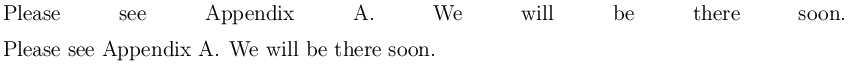
\includegraphics{linebreak}
\end{quote}
\end{htmlonly}

\subsection{�����Y��\index{�Y��}}

�Ĥ@���Y�ƤF�I�o�O�]���ڭ̧����S�������`�A�ҥH�A\LaTeX\ �N��o�Ǥ��e�����O�ި��������A�� \LaTeX\ ���w�ơA�ި��}�Y�O�|�Y�ƪ��C�n�ѨM�o�Ӱ��D�A�i����ؤ�k�G

\begin{enumerate}
\item �b�Ĥ@�椧�e�[�J \verb|\noindent|\index{noindent@\verb+\noindent+} �ӫ��� \LaTeX\ ���n�h�Y�ơC���O�o�u�@�Φb�U���O���a��A��L���Y�ƪ��a���٬O�|�Y�ơC
\item �b preamble �ϥ[�J \verb|\parindent=0pt|\index{parindent@\verb+\parindent+}�A�o���������媺�Y�Ƭ� {\tt 0pt}�A���M�A�o�N���ܥ��峣���n�Y�ƤF�C
\end{enumerate}

\section{�[�J���`���D\index{���`���D}}

�b \LaTeX\ ���Y�A�n�[�J���`���D��b�O�Ӯe���F�A�]�����h�ަr�骺�j�p�θm�񪺦�m�A�ɺޥ[�W�h�N��F�I\LaTeX\ �|���ڭ̦w�Ƥ@���C�ڭ̳o�̤��M�H {\tt report} ���O�ӻ����A�]�� {\tt article} ���O���Y�A�S�����A�u��A�Ω��²�檺�u��C

\begin{quote}
\begin{verbatim}
% example2.tex
\documentclass{report}
\begin{document}
This is the first experience of \LaTeX.
\chapter{Aesop Fables}
\section{The Ant and the Dove}

An ant went to the bank of a river to quench its thirst, and
being carried away by the rush of the stream, was on the
point of drowning.

A Dove sitting on a tree overhanging the water plucked a
leaf and let it fall into the stream close to her. The Ant
climbed onto it and floated in safety to the bank.

\section{The Dog in the Manger}

A dog lay in a manger, and by his growling and snapping
prevented the oxen from eating the hay which had been
placed for them.

``What a selfish Dog!'' said one of them to his companions;
``he cannot eat the hay himself, and yet refuses to allow
those to eat who can.''

\chapter{The Eagle and the Arrow}

An eagle sat on a lofty rock, watching the movements of a
Hare whom he sought to make his prey.

An archer, who saw the Eagle from a place of concealment,
took an accurate aim and wounded him mortally.
\end{document}
\end{verbatim}
\end{quote}

�sĶ�X�Ӫ����G�G

\begin{quote}
\url{http://edt1023.sayya.org/tex/latex123/example2.tex}\\
\url{http://edt1023.sayya.org/tex/latex123/example2.pdf}
\end{quote}

�Ъ`�N�L����ɭԷ|�Y�ơA����ɭԷ|�����C{\tt report} ���O�A�s���@���|�����A�p�G�Q�`�٤@�I�Ŷ��A�i�H���� {\tt article} ���O�A\verb|\chapter{}| ��� \verb|\section{}|�A��� \verb|\section{}| �N��� \verb|\subsection{}|�A�o�˴N���|�����A���e�N�|�s��U�h�F�C�j�a�i�H�յۧ� {\tt report} �令 {\tt article} �� {\tt book} �A���s�sĶ�@���A�ոլݵ��G���󤣦P�C

\section{�[�J title page ��T}
\label{sec:titlepage}\index{title page}

�o�O���������Ĥ@���A�ڤ]�����D�o�Ӥ���M���W���O����A�b \LaTeX\ ���Y�A�ڭ̴N�٬� title page�C�b \LaTeX\ ���зǮ榡�̡A�L�]�A�F���D�]title�^�B�@�̦W�r�]author�^�B����]date\index{date}�^�ηP�µ��]thanks\index{thanks}�^�C�n�`�N���O�A�b {\tt report/book} ���O�Atitle page �O�ۦ��@��W�����A���b {\tt article} ���O�̡A�L�O�M����s�_�Ӫ��C�ڭ̴N�H�W��������J�����峹���ҡA�n�ק諸�a��O preamble\index{preamble} �ϤΥ���Ϫ� \verb|\maketitle|\index{\verb=\maketitle=}�G

\begin{quote}
\begin{verbatim}
% example3.tex
\documentclass{report}
\title{Aesop Fables}
\author{Aesop\thanks{Thanks to the reader.}
       \and Nobody\thanks{Thanks to nobody.}}
\date{\today}
\begin{document}
\maketitle
This is the first experience of \LaTeX.
\chapter{Aesop Fables}
\section{The Ant and the Dove}
 ...
\end{verbatim}
\end{quote}

�ƪ��X�Ӫ����G�p�U�G

\begin{quote}
\url{http://edt1023.sayya.org/tex/latex123/example3.tex}\\
\url{http://edt1023.sayya.org/tex/latex123/example3.pdf}
\end{quote}

�ڭ̥i�H�o�{�A�o�@���O���s���X���A�q�U�@���}�l�~�O�Ĥ@���C�@�̥i�H���h�ӡA�ϥ� \verb|\and| ���O�ӳs���C������@�w�n���A�p�G�S�� \verb|\date{\today}| �o�ӫ��O�A���٬O������A���u��T�w�b���ѡC�p�G���e�L���A�L�|�۰ʧ��A���]�i�H��ʥ[ \verb|\\| �ӱj������A���ަp�󴫦�A��ӥy�l�O�~���ƦC���C\verb|\maketitle| �O�U�b����Ϫ��}�Y�A�p�G���U�o�ӫ��O�A���sĶ�ɤ��|��������~�A�u�O�N�S�� title page �F�C

\section{�[�J�ؿ��]Table of Contents�^}
\label{sec;toc}

�[�J�ؿ��]Table of Contents\index{Table of Contents}�^�� \LaTeX\ �Ө��A��O���ө��|���Ʊ��A�u�n�b����}�Y�[��
\verb=\tableofcontents=\index{tableofcontents@\verb=\tableofcontents=}
���O�N���F�I�̤W�����Ҥl�A�ק令�G

\begin{quote}
\begin{verbatim}
% example4.tex
\documentclass{report}
\title{Aesop Fables}
\author{Aesop\thanks{Thanks to the reader.}
       \and Nobody\thanks{Thanks to nobody}}
\date{\today}
\begin{document}
\maketitle
\tableofcontents
This is the first experience of \LaTeX.
\chapter{Aesop Fables}
\section{The Ant and the Dove}
 ...
\end{verbatim}
\end{quote}

�ƪ��X�Ӫ����G�p�U�G

\begin{quote}
\url{http://edt1023.sayya.org/tex/latex123/example4.tex}\\
\url{http://edt1023.sayya.org/tex/latex123/example4.pdf}
\end{quote}

�o�̤d�U�n�`�N���O�A\verb|\tableofcontents| �n�[�b \verb|\maketitle| ���᭱�A�_�h�ؿ��|�L�b title page ���e�C�ӥB�n\textcolor{red}{\bf �sĶ�⦸}�C�Ĥ@������ {\tt example4.toc}�A�M��ĤG���sĶ�A��ڳo�� {\tt toc} �ɡA�u���s�J�ؿ��C

�ؿ��O�]�A�Ϫ��ؿ����]List of Figures, List of Tables�^�A���ڭ̥ثe�٨S���ͨ�Ϫ����ƪ��A�]���Ȯɲ��L�A���ͨ�ɦA�Ӭݭn�p��[�J�Ϫ��ؿ��C

\section{�[�J�K�n�]abstract�^}
\label{sec:abstract}\index{abstract}

�o���@�w�|���A�p�G�n�[�J���ܡA�i�ϥ� {\tt abstract} ���ҡA�b�o�����Ҥ����峹�A���k�|�Y�ơC�n�`�N���O�A�u�� {\tt article/report} ���O�~�� abstract�A{\tt book} ���O����ϥγo�����ҡC

\begin{quote}
\begin{verbatim}
% example5.tex
\documentclass{report}
\title{Aesop Fables}
\author{Aesop\thanks{Thanks to the reader.}
       \and Nobody\thanks{Thanks to nobody}}
\date{\today}
\begin{document}
\maketitle
\begin{abstract}
The tale, the Parable, and the Fable are all common and popular
modes of conveying instruction. Each is distinguished by its own
special characteristics.
\end{abstract}
\tableofcontents
\chapter{Aesop Fables}
\section{The Ant and the Dove}
 ...
\end{verbatim}
\end{quote}

�ƪ��X�Ӫ����G�p�U�G

\begin{quote}
\url{http://edt1023.sayya.org/tex/latex123/example5.tex}\\
\url{http://edt1023.sayya.org/tex/latex123/example5.pdf}
\end{quote}

{\tt report}\index{\texttt{report}} ���O���K�n�ۦ��@���A���s���X�A�B���|�s�J�ؿ����A�o�M�@�몺�פ�榡�i��|���@�ˡA�ϥήɽЪ`�N�C{\tt artcile}\index{\texttt{artcile}} �����O�h���M�O�M����۳s���A�|�X�{�b�峹���D����C

{\tt abstract} �M summary\index{summary} �b���������פ�O���Ϥ����A�q�` abstract �b��e�Fsummary �h�b���C���ثe�@��ʪ��峹�h�S���o�˰ϧO�A�q�q�����u�K�n�v�C�q�`�A�K�n���Y�O���ε��ѡB�L�椬�ѷӤ]���ϥΤ����Ϫ����C


\section{�[�J����}
\label{sec:footnote}\index{����}

�b \LaTeX\ ���Y�A���ѥi����ؤ覡�A�@�جO�}���]footnote�^\index{footnote}\index{�}��}�A�@�جO����]marginal note�^\index{marginal note}\index{���}�C�q�` \LaTeX\ ���}���w�]�O�Ѫ��ԧB�Ʀr�b�s���A�m�󭶩����C�b�S�����]part�^�����ΤU�A\texttt{report/book} ���O�A�s���C���|�q�Y�_��A\texttt{article} ���O�h�|�s��A�ӥB�A�|�ϥ� \texttt{footnotesize}\index{footnotesize@\texttt{footnotesize}} ���r��L�X�C����h���s���A�r��O���`�j�p�C

\subsection{�}���]Footnote�^}

�b�ҭn�[�������Ӧr��A�ϥ� \verb|\footnote{}| ���O�Y�i�A�ѻ�����r�N�g�J�j�A�������A�@�� \LaTeX\ �����O�b�������M�����@�ΡA�|�L�b�����������A�H�p�@�I���r�ӦL�X�A�å[�W�s���C�H�U�ڭ̴N�ոլݦb Dove �o�Ӧr�Ӱ��}���C�Ъ`�N�ADove �o�Ӧr�M \verb|\footnote{}| �����O�S���ťժ��C

\begin{quote}
\begin{verbatim}
% example6.tex
\documentclass{report}
\title{Aesop Fables}
\author{Aesop\thanks{Thanks to the reader.}
       \and Nobody\thanks{Thanks to nobody}}
\date{\today}
\begin{document}
\maketitle
\tableofcontents
This is the first experience of \LaTeX.
\chapter{Aesop Fables}
\section{The Ant and the Dove}

An ant went to the bank of a river to quench its thirst, and
being carried away by the rush of the stream, was on the
point of drowning.

A Dove\footnote{Pigeon, an emblem of peace.}
sitting on a tree overhanging the water plucked a
leaf and let it fall into the stream close to her. The Ant
climbed onto it and floated in safety to the bank.
 ...
\end{verbatim}
\end{quote}

�ƪ��X�Ӫ����G�p�U�G

\begin{quote}
\url{http://edt1023.sayya.org/tex/latex123/example6.tex}\\
\url{http://edt1023.sayya.org/tex/latex123/example6.pdf}
\end{quote}

\subsection{����]Marginal note�^}

����u�O�� \verb|\footnote{}| ���� \verb|\marginpar{}|\index{marginpar@\verb=\marginpar=} �Ӥw�A���e���M�g�J�j�A�����C���M�}�����@�˪��O�A�L�S���s���]�]���N�b����A�L�����n�^�A�L���r��]���|�p�@���A�M���媺�r��j�p�O�@�˪��A�o�b�᭱�Q�ר�r�����ɭԷ|�ͨ�p����ܦr�骺�j�p�C

\begin{quote}
\begin{verbatim}
% example7.tex
\documentclass{report}
\title{Aesop Fables}
\author{Aesop\thanks{Thanks to the reader.}
       \and Nobody\thanks{Thanks to nobody}}
\date{\today}
\begin{document}
\maketitle
\tableofcontents
This is the first experience of \LaTeX.
\chapter{Aesop Fables}
\section{The Ant and the Dove}

An ant went to the bank of a river to quench its thirst, and
being carried away by the rush of the stream, was on the
point of drowning.

A Dove\marginpar{Pigeon, an emblem of peace.}
sitting on a tree overhanging the water plucked a
leaf and let it fall into the stream close to her. The Ant
climbed onto it and floated in safety to the bank.
 ...
\end{verbatim}
\end{quote}

�ƪ��X�Ӫ����G�p�U�G

\begin{quote}
\url{http://edt1023.sayya.org/tex/latex123/example7.tex}\\
\url{http://edt1023.sayya.org/tex/latex123/example7.pdf}
\end{quote}

\section{�r���������վ�}
\index{�r��!�����վ�}

\TeX/\LaTeX\ ���r���t�κ�O�۷��������A�o�̤��h�ͨ䤤��z�A���b�ϥΪ̪����סA�ڭ̥u�n���D���ϥδN��F�C�b�o�̡A�ڭ̻��r���]font�^\index{font}\index{�r��}�A�����O�r���������@���`�١A�κ٬��r��\index{�r��}�A�b�r���Ϊ����ɭԡA�ڭ̴N�٬��r�Ρ]font shape�^\index{font shape}\index{�r��}�C

\LaTeX\ �ϥΪ��r����r����A�H�ثe�s������ \LaTeX\ �Ө��A�O�ϥ� 1993 �~�o�檺 NFSS(New Font Selection Scheme) �ĤG�����зǡC���M�A���M�O�إߦb \TeX\ �r�������¦�W���A�o�w�W�X�o�g�峹���d��C

\subsection{\LaTeX\ ��r�����ݩʴy�z}
\label{subsec:font-attr}\index{�r��!�ݩʴy�z}

�b \LaTeX\ �̡A���r�����y�z�A�ϥΤF�����ݩʨӻ����A�o�����ݩʡA�]�O \LaTeX\ �������`�n�ϥΨ쪺�ѼơA�ƦܬO���~�T���Хܦr���ӷ����ɭԡA�|��r�����o���ݩʵ���ܥX�ӡC

\begin{enumerate}
\item �r���s�X�]font encoding�^\index{font encoding}\index{�r��!�r���s�X}\\
�o�̩ҿת��r���s�X�A�����O�U�ӭӧO���r�b�@�Ӧr�����Y���ƦC���ǤΦw�Ƥ覡�C��l�� \TeX\ �r���s�X�ڭ̴N�٬� OT1(Old \TeX\ text encoding)\index{OT1}�A�o�O�w�]���A�p�G�������w�r���s�X�A���ҨϥΪ��N�O OT1 �s�X�C�b�ثe�s�@�N���r���s�X���Y�A�r���w�Ƥ覡�Τ��e�M OT1 ���@�ˡA�Ҧp
T1\footnote{�����W�٬O Cork's \TeX\ extended text encoding �S�٬� Text Companion encoding�C�o�̪� T1 �M Type 1 �r���W��\index{�r��!�r���W��}�L���A�L�O�r���s�X�覡�A�L��r�����Y�����@�ǭ����Ÿ��r����W�����@�ӳ�W���r�A�ӫD�p OT1 �O�Ѥ@��r���M�����Ÿ��զX�Ӧ��C}\index{T1}�A�o�b���ᴣ����ܦr���s�X�ɷ|�A�ͨ�A�ڭ̥ثe�N���h�վ�r���s�X�A�ϥιw�]�� OT1�A��L���s�X�o�̴N���h�ͤF�C

\item �r�ڡ]font family�^\index{font family}\index{�r��}\\
���P�@�]�p�������r�����X���W�١A�Ҧpù���r�ڡ]roman�^\index{roman}\index{ù���r��}�B���r���r�ڡ]typewriter�^\index{typewriter}\index{���r���r��}�����A�q�`�e���|�a�W�s�@�өλs�@�H���W�١A�Ҧp Knuth\index{Knuth} �б³]�p���A�٬� `Computer Modern Roman'\index{Computer Modern Roman}�AAdobe ���q�s�@��ù���r�ں٬� `Adobe Times'\index{Adobe Times}�C�ڭ̹w�]�ϥΪ��A���M�N�O Knuth �б©ҳ]�p�� Computer Modern fonts�C�H�U���@�ǨҤl�G

\begin{quote}
\begin{tabular}{>{\tt}ll}
²�� & �N���N�q \\
\hline
cmr  & Computer Modern Roman \\
cmss & Computer Modern Sans Serif \\
cmtt & Computer Modern Typewriter 
\end{tabular}
\end{quote}

\item �r���t�C�]font series�^\index{font series}\index{�r��!�r���t�C}\\
�o�O���r���� weight�]�D�G�^�� width�]����^�ӰϤ����C�Ҧp�ʡB�Ӧr��A�@��ڭ̥��`�Ϊ��O medium�A����h�O bold�C�H�U�O�@�ǨҤl�G

\begin{quote}
\begin{tabular}{>{\tt}ll}
²�� & �N���N�q \\
\hline
m  & medium \\
b  & bold \\
bx & Bold extended \\
sb & Semi-bold \\
c  & Condensed
\end{tabular}
\end{quote}

\item �r�Ρ]font shape�^\index{font shape}\index{�r��}\\
�o�ӱ��͸q�A�N�O�r���Ϊ��C�Ҧp�N�j�Q����]italic�^\index{italic}\index{�N�j�Q����}�B����]slant�^\index{slant}\index{����}�Bsmall caps\index{small caps} �����C�H�U�O�X�ӨҤl�G

\begin{quote}
\begin{tabular}{>{\tt}ll}
²�� & �N���N�q \\
\hline
n  & ���`�r�]normal�^�A�� upright �� roman \\
it & Italic \\
sl & Slanted \\
sc & Small Caps \\
\end{tabular}
\end{quote}

\item �r���j�p�]font size�^\index{font size}\index{�r��!�r���j�p}\\
�w�]���r���j�p�O 10pt�]10 point�^�A�Q�I�r�C���[��쪺�ܡA�w�]���N�O pt�C�Ъ`�N�A�D�з� \LaTeX\ ���O���w�]�r���j�p�i��|���@�ˡC
\end{enumerate}

�ڭ̹�r���n�վ���ܪ��A�N�O�o�Ǧr���ݩʪ��]�w�ȡC\LaTeX\ �w�]�w�n��K�����O���ڭ̨ϥΡC

\subsection{�վ�r�ڡB�r���t�C�B�r�Ϊ����O}
\label{subsec:font-command}

%begin{latexonly}
\linespread{1.0}
\small
\begin{tabular}[\textwidth]{lllll}
    & �r�� & �зǫ��O & �ŧi�����O�]���ҡ^& �¥Ϊk \\
\hline
�r  & \textup{textup} & \verb|\textup{textup}| & \verb|{\upshape textup}| & \\
��  & \textit{italic} & \verb|\textit{italic}| & \verb|{\itshape italic}| & \verb|{\it italic}| \\
    & \textsl{slant}  & \verb|\textsl{slant}|  & \verb|{\slshape slant}| & \verb|{\sl slant}| \\
    & \textsc{small caps} & \verb|\textsc{small caps}| & \verb|{\slshape small caps}| & \verb|{\sc small caps}| \\
\hline
�t & \textmd{medium} & \verb|\textmd{medium}| & \verb|{\mdseries medium}| &  \\
�C & \textbf{boldface} & \verb|\textbf{boldface}| & \verb|{\bfseries boldface}| & \verb|{\bf boldface}| \\
\hline
�r & \textrm{roman} & \verb|\textrm{roman}| & \verb|{\rmfamily roman}| & \verb|{\rm roman}| \\
�� & \textsf{sans serif} & \verb|\textsf{sans serif}| & \verb|{\sffamily sans serif}| & \verb|{\sf sans serif}| \\
   & \texttt{typewriter} & \verb|\texttt{typewriter}| & \verb|{\ttfamily typewriter}| & \verb|{\tt typewriter}| \\
\end{tabular}
\linespread{1.36}
\normalsize
%end{latexonly}

\begin{htmlonly}
\begin{quote}
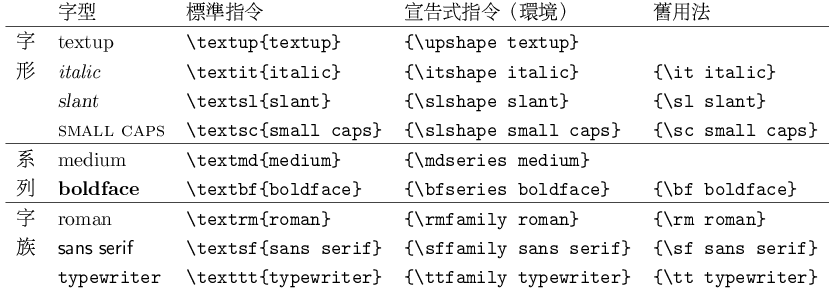
\includegraphics{fntshape}
\end{quote}
\end{htmlonly}

���O�~�F�@���A�o�O����i�`���C�䤤 upright, medium, roman ���O�@�˪��A�o�O�@�몺���`�r�A�N�����·Хh�]�w�L�F�A���D�O�n�b�S�w�r���d����Y�A���s���ܦ����`�r��C�q�e���һ���²�٪��r��A�A�M text, family, series, shape �h�t��ӨϥΡA�o�˥u�n�O�o²�ٴN��F�A�Ҧp�Gitalic ���N�O \verb|\textit{}|�C���M�]�i�H�ϥΡu���Y�B�v���¥Ϊk�A���o�]���O���򰽦Y�B�A�L�O��l Plain \TeX\index{Plain \TeX} �ҩw�q���A�b�ª��� \LaTeX\ 2.09 �]�ۮe�L�Ӫu�ΡA�å[�H�X�R�C���p�G�ϥ��¥Ϊk�A�����ɲզX�������ܮɥi��|�L�ġA�Ҧp�ʱ���o�ز���M����]�w�V�X�ɡA�N�L�k���Ͳʱ���F�A�o���٬O�o�ĨĨϥΥ��μз� \LaTeX\ �����ܪk�C

�n�`�N���O�A�j�A������m�A�ŧi�������O�A��ӧ@�νd��O�s���O�@�_�]�����A�L�i�H�������ҨӨϥΡA�Ҧp \verb|\begin{itsahpe}|, \verb|\end{itshape}|�A�o�˦b�o�����Ҥ�����r�N�q�q�|�ϥ� italic ����A�]�i�H���[�ѼƨϥΡA�Ҧp \verb|\itshape|�A�o�˥H�U����r�q�q�|�ϥ� italic ����A���ܥt�@�ӧ��ܦr�������O�X�{����C�зǫ��O���@�νd��h�O�������O���@�ӰѼơA�o�ǰѼƬO�X�{�b���O�᪺�j�A�������C�{�b�N�ӹ�ڽsĶ�ӨҤl�լݬݡG

\begin{quote}
\begin{verbatim}
% example8.tex
\documentclass{report}
\title{\bfseries Aesop Fables}
\author{Aesop\thanks{Thanks to the reader.}
       \and Nobody\thanks{Thanks to nobody}}
\date{\today}
\begin{document}
\maketitle
\tableofcontents
\chapter{Aesop Fables}
\section{The \textsl{Ant} and the \textsl{Dove}}

\itshape
An antwent to the bank of a river to quench its thirst, and
being carried away by the rush of the stream, was on the
point of drowning.
\upshape

A \textsl{Dove} sitting on a tree overhanging the water plucked a
leaf and let it fall into the stream close to her. The \textbf{\textsl{Ant}}
climbed onto it and floated in safety to the bank.

\section{The {\it Dog}\/ in the Manger}

A \textbf{\textit{dog}} lay in a manger, and by his growling and snapping
prevented the oxen from eating the hay which had been
placed for them.

``What a selfish Dog!'' said one of them to his companions;
``he cannot eat the hay himself, and yet refuses to allow
those to eat who can.''

\chapter{The \textsc{Eagle} and the Arrow}

An \textsc{eagle} sat on a lofty rock, watching the movements of a
Hare whom he sought to make his prey.

An archer, who saw the \textsc{Eagle} from a place of concealment,
took an accurate aim and wounded him mortally.
\end{document}
\end{verbatim}
\end{quote}

�ڭ̧� title page\index{title page} �����D�令����]�Ъ`�N�A�ŧi�����¥Ϊk�A�j�A���O����O�M��r��ӬA�����^�A�� Dove �令 slant ����A�� dog �令 italic �ʱ���\footnote{�Ъ`�N�A�o��ر���O���@�˪��Aslant �O�@�륿�`���r�A�u�O��L�ɱ׭Ө��צӤw�A�� italic �h�O�t�@�ؿW�S���r���]�p�C}�A�� ant �令 slant �ʱ���A�� eagle �令 small caps�C�ѩ󳹸`���D�쥻�N�|�ഫ������A�ҥH���`���D�������A����N�������Ƴ]�F�C

���o�̵o�{�Ҥl�̲ĤG�����D���� Eagle �èS�����ܦr��A�ӥB�H {\tt latex} �sĶ�ɷ|���ͥH�U�����~�]�o�ǰT���]�|�b {\tt example8.log} �����^�G

\begin{quote}
\begin{verbatim}
  ...
LaTeX Font Warning: Font shape `OT1/cmr/bx/sc' undefined
(Font)              using `OT1/cmr/bx/n' instead on input line 4.
  ...
LaTeX Font Warning: Some font shapes were not available, defaults substituted.
  ...
\end{verbatim}
\end{quote}

�{�b�ڭ̬ݨ�F�e���ҽͪ��ݩ�²�١A�o�b \LaTeX\ �N�|�ϥγo���ݩʨӪ��ܦӵo�X�T���A�o�� \verb|OT1/cmr/bx/sc| �N���ܤF OT1 �s�X�AComputer Modern Roman �r�ڡABold extended �t�C�A�ӥB�O small caps �Ϊ����r���A���~�T����ܡA�L�èS���w�q�A�]���A�o�Ӧr���N�|�ϥιw�]���r���ӥN���A�o�̴N�O�H n ���`�Ϊ��� bx �t�C�r���Ӵ��N�C�ҥH�A�r�����O�ä��O���i�H�H�N�զX���A���ǬO�ڥ��N�S���o�ئr���A���ǫh�O�S���Υ����h�w�q�n�A�o�� \LaTeX\ �N������r�F�A���O��ߡA���h�N�O�ϥιw�]���r���}�F�I

�t�@�ӫܩ_�Ǫ��a��A�N�O�Ĥ@���B�ĤG�`�����D�A������O \verb|{\it Dog}\/ in the...}|�H�o�Ӵ��J�� \verb|\/| �O����F��H�o�O \TeX\ �t�νվ����r�]�]�A iatlic �� slanted�^�M���`�r�������ťժ��@�ӫ��O�A�٬� italic correction\index{italic correction}�C�o�ˡA�b����r�M���`�r�������ťդ~�|���`�C���������L��������O�S���[�o�ӽվ�O�H�o�O�]�� \LaTeX\ �����b�]�p�ɴN���Ҽ{��o�Ӱ��D�A�ҥH \verb|\textit{}| �o���зǫ��O���|�۰ʽվ� italic correction�A�����ѧڭ̤�ʽվ�C

�t�~�A���`���D���N�|�۰��ഫ������A���D�W�� dog ������S���ܲ���H�o�b�e��������L�A�o���¥Ϊk���ɬO�L�k�ƦX�ϥΪ��A����S���骺���O�|�Τ��W�ӡC�]���A��ij�ɶq�ϥ� \LaTeX\ ���Ĥ@�ؼзǫ��O�ӧ��ܦr���C�ϥ� \verb|{\it ...}| �� \verb|{\itshape ...}|\footnote{�ŧi�����O�i�H�ƦX�ϥΡA�����M�|�ݭn��ʰ� italic correction�C} �o�ث��O���ܡA�N�o�ɮɪ`�N italic correction �����D�A�]�o�`�N�O�_�i�H�ƦX�ϥΫ��O�����D�A�ҥH�A�٬O���n���i���n�C:-)

��U�O�ƪ��X�Ӫ����G�G

\begin{quote}
\url{http://edt1023.sayya.org/tex/latex123/example8.tex} \\
\url{http://edt1023.sayya.org/tex/latex123/example8.pdf}
\end{quote}

\subsection{�۹�r���j�p���վ�}

���U�ӽͳ̫�@�Ӧr���j�p�ݩʪ��վ�A�o�b�ϥΤW�����¡A�u�n���D���O�N�i�H���W���ӨϥΡC���O \TeX/\LaTeX\ �t�Τ��A�ͨ�r���A���Y�@��a�p�A�Ҧp�e���ͨ쥿�`������r���j�p�O 10pt�A�{�b�p�G�Q�s�@�����A�ݭn 64pt ���r���ɭԴN�|�o�{�A�]���X�ӤF�I���` \LaTeX\ ���w�q�A�r�����j�p�d��O�b 5--24.88pt �����A�W�X�o�ӽd�򪺦r�ݭn��L�� package �������C\footnote{�o�O \LaTeX\ ���������w�q�����D�A�]���L�D�n�O�w��@��ʤ��ή��y�A\TeX\ ��������O�A�i�H���r����j�� 2047pt�C}

�o�̧ڭ̥��Ӭݬݤ��� 10pt �ɦU�ئr���j�p���O�B��ڨҤl�Ψ�j�p�]�o�O�۹�j�p�A�|�H����w�]�r���j�p�Ӧ۰ʽվ�^�G\footnote{�Ъ`�N�A���� pdf �榡����ϥ� 12pt �r���j�p�A�C���Ψ䤤���Ҥl�A�O�ѥt�~ 10pt �w�]�r���j�p�һs�@�� eps ���ɤޤJ�A�H�K���u�C}

\begin{quote}
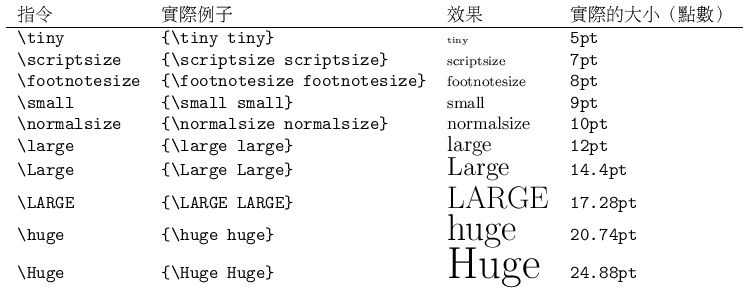
\includegraphics{fntsize}
\end{quote}

�o�Ǧr���j�p���O�]�i�H�������ҨӨϥΡA�Ҧp�G

\begin{quote}
\begin{verbatim}
\begin{small}
  ���夺�e
\end{small}
\end{verbatim}
\end{quote}

�o�˥Τ]�O�i�H���C

\subsection{����r���j�p���վ�}

�q�`�r�����j�p\index{�r��!�r���j�p}�A�ϥΤW�@�`�һ����۹�r���j�p�ӽվ�|�����K�A�ӥB����Ӫ������t�X�]�|�������A�Ҧp��Z�]�|��۰��A�����վ�A�p�G�ۦ�ε���r���j�p����k�ӽվ�r���j�p���ܡA�`�`�|�y����Z���@�P�����ΡA�]���A�p�D���n�A���ɶq�קK�C

�����ɭԴN�O�ݭn���o�˪��վ�A�Ҧp����ʭ����r���j�p�A�a�ϬO \LaTeX\ �w�]���̤j�r���]ı�o�y�p�F�I�A�o�N�n�t�~�ޤJ package �վ�F�C

�o�̧ڭ̨ϥ� \textsf{type1cm}\index{type1cm@\textsf{type1cm}} package �ӽվ�C���M�A�o�ϥ� Type 1 �r���A�~�i�H�F��L�q��j�B�Y�p���ت�%
\footnote{\LaTeX\ �t�Τ����r����j�A�b 10pt �H�W�A�O�H 1.2 �����Ƭ�����ө�j���A�]���A���� 10pt ���r���j�p���ܡA���|�� 13pt �o�ؤj�p���r���A\LaTeX\ �|��γ̬۪�j�p���r���Ӵ��N�C}%
�A�ӳo�� package �]�O�t�X Type 1 �r���ϥΪ��C�ӧO��j�� pk �I�}�r�A�o�̴N���Q�פF�A�ثe���j������ Computer Modern �r�����w�� Type 1 �� free �����A�ӥB�U�� \TeX\ distribution ���|���W�A�ϥΤW�|����K�C�H�U�O \textsf{type1cm} ���ϥΤ�k�G

\begin{quote}
\begin{verbatim}
  ...
\usepackage{type1cm}
  ...
\fontsize{�r���j�p}{��Z�j�p}\seclectfont
  ...
\end{verbatim}
\end{quote}

�ٰO�o�p��ޥΥ����M��\index{�����M��}�ܡH�аѦҲ� \ref{ch:syntax} ���B�� \ref{sec:struct} �`�A�� \ref{subsec:preamble} �p�`�������C

�䤤���u�r���j�p�v�N�O�ҭn���w���j�p�A�q�`�H pt �����A���M�A�n�ϥΨ�L���]�O�i�H�C�u��Z�j�p�v�]�O�n�@�֫��w�A���i�ٲ��C�̫᪺ \verb|\seclectfont| �O���L�o�ͧ@�Ϊ��N��A\LaTeX\ ��������r�������C�����O�A�n�U \verb|\seclectfont| ��~�|�@�ΡA\verb|\fontsize{}{}|\index{fontsize@\verb=\fontsize=} ���O�䤤���@�C

\section{���ӦC}

����O���ӦC\index{���ӦC}�H�@�� \LaTeX\ �J��˱׽u\index{�˱׽u}�|�{���O�@�ӫ��O���}�l�A�p�G�s��ӫ��O���n�L�X���ɭԩO�H�o�ɴN�n�Ψ���ӦC�����O�����ҤF�C

\subsection{���ӦC���O}

�p�G�u�O�@�p�q����r�n���ӦC�A���ϥΫ��O�|�����K�A�o�ӫ��O�N�O \verb+\verb|��r���e|+\index{verb@\verb=\verb=}�A�䤤�� \verb+|+ �o�ӲŸ��i�H�ϥΨ�L�D�r�����Ÿ��N���A�u�n�e��ۦP�N��F�A�Ҧp�G\verb|\verb+��r���e+| �o�ˤ]�O�i�H���C

\subsection{���ӦC����}

�p�G�O�@��q�����e�n���ӦC���ܡA�ϥ����ҷ|�����K�A���K�O {\tt verbatim} ���ҡC���ެO���@�ح��ӦC�����ΡA�w�]�O�ϥΥ��r���r�ڪ��r������ܪ��C���U�O�@��²�檺�Ҥl�A�������ӦC���O�����Ҫ��ϥΡG

\begin{quote}
\begin{Verbatim}[commandchars=+\[\]]
% example9.tex
\documentclass{article}
\begin{document}
The example of \verb|\verb{}| command and \texttt{verbatim} environment.

\section{\textbackslash{}\texttt{verb} command}

When you want to express you home directory, you can \verb|echo $HOME|
varient to display your home directory in your sh script.

\noindent
\verb*|This is    4 space here.|

\section{\texttt{verbatim} environment}

Here is a sh script to determine if on GNU/Linux system.

\begin{verbatim}
#!/bin/sh
Date=`date '+%y%m%d'`
if [ `uname` = Linux ]
then
  Mail=/var/spool/mail/edt1023
  Target=/mnt/hd
else
  Mail=/var/mail/edt1023
  Target=/mnt/pub
fi
\end{verbatim}
\end{document}
\end{Verbatim}
\end{quote}

�o�̷|�o�{�@�ǩ_�Dz{�H�A�Ҧp
\texttt{\textbackslash{}verb*}
���ӬP���O����N��O�H�N�O���ťեH
%begin{latexonly}
\verb*| |
%end{latexonly}
\begin{htmlonly}

\includegraphics{blank}
\end{htmlonly}
���覡���ܥX�Ӫ��N��A{\tt verbatim} ���Ҥ]�O�i�H�o�˨ϥΡC�Ҧp {\tt example9} �����G

\begin{quote}
\begin{verbatim}
\verb*|This is    4 space here.|
\end{verbatim}
\end{quote}

�]�i�H�g���G

\begin{quote}
\begin{Verbatim}[commandchars=+\[\]]
\begin{verbatim*}
This is    4 space here.
\end{verbatim*}
\end{Verbatim}
\end{quote}

�t�O�b��A���Ҫ��W�U��|�h�ťX�Ӫťզ�X�ӡC

�t�~�A���D�����򤣨ϥ� \verb+\verb|\verb|+ �N�n�F�O�H��]�O���ӦC�����O�M���ҳ����������L���O���ѼơA���D�����N�O�@�ӫ��O�A�ҥH \verb+\verb+ ����b���Y�C

�ϥ� \verb|\textbackslash|\index{textbackslash@\verb=\textbackslash=} �o������ԭz�A�Ӥ��� \verb|$\backslash$| �o��²�檺�覡�A��]�O�o�Ӥ�Z���ϥ� \LaTeX{}2{\tt HTML} ���ন HTML �榡�A�ϥ� \LaTeX\ �����N���ܪk�|�ন�@�몺�Ÿ��A���ϥΫ�̪��覡�h�|�ন���ɡA�ҥH�o�̴N�ϥ� \LaTeX\ �����N���ܪk�F�C

���U�O�ƪ��X�Ӫ����G�G

\begin{quote}
\url{http://edt1023.sayya.org/tex/latex123/example9.tex}\\
\url{http://edt1023.sayya.org/tex/latex123/example9.pdf}
\end{quote}

\section{�[�J����}

�o�̥u�����p��ϥ� \textsf{CJK}\index{CJK@\textsf{CJK}} package �����ΡA��]�O�@�� \TeX\ distribution �|���W�]���ǵo��M��èS�����W�A�o�ɥu�n�ۦ�w�ˤF�^�C\textsf{CJK} package �O�⤤�媺�����]�b�@�����Ҹ��Y�A�b�o�����Ҥ��N�i�H�ϥΤ���A���}�o�����ҴN�S�^�_��쥻���^�����ҡA���U�ѨҤl�ӻ����C

\begin{quote}
\begin{verbatim}
\documentclass{article}
\usepackage{CJK}  % �ϥ� CJK �����M��
\begin{document}
% �i�J CJK ���ҡA�èϥ� Big-5 �X�� hwmm �o�Ӧr��
\begin{CJK}{Bg5}{hwmm}
\section{CJK �����M��}
�o�O�@�Ӵ��աA���� CJK package �����աC
\section{��᷽�O�`��}
��U�A�׳q�H�F�_��ƤQ�B�A�ŵM�}�ԡC�g�a���m�A�Ϊ��k�M�C���}�СB�����B%
��B�ˤ��ݡA�魯��q�A�����ۻD�C�䤤���Ӻا@�A�k�k��ۡA�x�p�~�H�F���v�B%
���ԡA �éɵM�ۼ֡C�����H�A�D�j��A�ݩұq�ӡF�㵪���A�K�n�ٮa�A�]�s�B�����B%
�@���C�����D�����H�A�w�ӰݰT�C�ۤ��G�u���@�ׯ��ɶáA�v�d�l���H�Ӧ����ҡA%
���_�X�j�F�E�P�~�H���j�C�v�ݤ��O��@�F�D�������~�A�L���Q�B�ʡC���H�@�@%
���㨥�һD�A�Ҽ۱{�C�l�H�U�_���ܨ�a�A�ҥX�s���C���Ƥ�A��h�C�����H�y%
���G�u�������~�H�D�]�C�v
\end{CJK}
\end{document}
\end{verbatim}
\end{quote}

�N�o��²��C�u�O�sĶ�n��� {\tt bg5latex}\index{bg5latex@\texttt{bg5latex}} �Ӥ��O��Ӫ� {\tt latex} ���O�A�o�O���F�׶}�ڭ� Big-5 �X���@�ǯS���X�����Y�A�ٰO�o����C��̫�n�[�Ӧʤ��� \verb|%|\index{%@\verb=%=} �ܡH�o�ˤ~���|���J�^�媺�r���ťաC�sĶ�n���Ҥl�p�U�G

\begin{quote}
\url{http://edt1023.sayya.org/tex/latex123/example10.tex}\\
\url{http://edt1023.sayya.org/tex/latex123/example10.pdf}
\end{quote}

�ԲӪ� \textsf{CJK} package ���ϥΤ��廡���A�аѦ� \textsf{CJK} package �Ҫ������Ρq�ڪ� CJK�r�@��G

\begin{quote}
\url{http://edt1023.sayya.org/tex/mycjk/mycjk.html}\\
\url{http://edt1023.sayya.org/tex/mycjk/mycjk.pdf}
\end{quote}


% ``�j�a�Ӿ� LaTeX'' LaTeX ��Z space.tex
% Copyright (c) 2004  Edward G.J. Lee <edt1023@info.sayya.org>
%
% �b���H�� GNU Free Documentation License 1.2 �ΥH�᪺�����W�d���U�A
% ���\�����B���G�έק�C���쪩�v�B���v�n�����o�����C
%
% �����G�����A�t�� fdl.tex�A���e�� GNU FDL ���W�d���C�p�G�򥢡A�i��
% http://www.gnu.org ���o�A�μg�H�ܦۥѳn�����|(Free Software Fundation)
% �����C
% 9 Temple Place - Suite 330, Boston, MA 02111-1307, USA.
%
% $Id: space.tex,v 1.23 2004/03/07 12:20:47 edt1023 Exp $
%
\chapter{�Ŷ��P��m}
\label{ch:space}

�e�@��������L�A�Ƿ|����Ŷ��N�Ƿ|�ƪ��F�IKnuth\index{Knuth} �б¦b�L�� \textit{The \TeX{}book}\index{The TeXbook@\textit{The \TeX{}book}} �@�Ѥ��]���ήe�ϥ� \TeX\ �ƪ������ΡG�@�Ӫ����N���@�ӧt�������]glue\index{glue}�^�������A�M��C�@�ӭn�ƪ������e�N�O�U�ؤ��P�� box\index{box}�A�b�o�� box �٨S���T�w���T��m�ɡA���O�i�H���ʪ��]�����٨S�����^�A�@���ƪ������A�����N���F�A��O�C�� box ����m�N�T�w�L�k�A���ʤF�A���D�S�q�Y�A�ӡC

�@�Ӧr���B�@�ӳ�r�B�@�ӥy�l�B�@�Ӭq���B�@�ӲŸ��B�@�ӹϧΡB�@�Ӫ��泣�i��c���@�� \TeX\ �� box�A�Ʀ� box ���٦� box �����ΡC�o���Q�Q�ת��A�N�O�o�� box �p��w�m�L�̨쥿�T����m�A���C�� box �������Ŷ�����F����n�B�A�ҥH�A�쩳�O�b���� boxes ���ݩʡB��m�A�٬O�վ� glue ���Ŷ��A�N�ݦU����h�ݫݤF�]�Ъ`�N�Abox ���@�w�O�i�����I�b \TeX\ ���Y�Aglue �O�i�H�վ㪺�C�^�C

�ڭ̫e���ҰQ�ר쪺�^��y�I��ťժ��վ�Bitalic correction\index{italic correction}�B\verb|\linespread|\index{linespread@\verb=\linespread=} �� \verb|\parindent|\index{parindent@\verb=parindent=} �o�dz��O�b�վ� glue�C�q�`�A�b \LaTeX\ �t�θ��Y�A���w���`�`���|�O����T�w���A�|�����ΰ��p���ת��۰ʷL�աA�o�O�����Ŷ��t�m�W���ݭn�C

\section{\LaTeX\ ���ϥΪ��׶q���}
\label{sec:units}

�n��T�y�z�M�վ� \LaTeX\ �����Ŷ��Φ�m�A�ڭ̥��ݭn���ӼзǪ��׶q���C�H�U���O�b \LaTeX\ �`�|�Ψ쪺���C�o�̦�������ά۹��줧���A���D���n�A���M�A�@��O��ij�ϥά۹���A��]�O�A�L�|�H�ۤ�Z�r���j�p���ܮɸ�۰��A�����վ�C���M�A�b�����D��T�B�T�w�j�p����ܮɡA�N�o�ϥε�����F�C

�o�̦p�G�O�\�� HTML �榡�����A�Хt�Ѧ� PDF �榡�����A�H�K���ܤW���u�C�H�U���椤�ҵe�X�Ӫ����׶ȨѰѦҥΡC

\subsection{������}
\index{������}

%begin{latexonly}
\begin{quote}
\begin{tabular}{>{\tt}lll}
���W�� & �N�q & ���� \\
\hline
pt & point, $1/72.27$~inch & \drawwidth{1pt} \\
bp & Adobe big point, $1/72$~inch & \drawwidth{1bp} \\
pc & pica, 12pt & \drawwidth{1pc} \\
mm & millimeter, $1/25.4$~inch & \drawwidth{1mm} \\
cm & centimeter, 10mm & \drawwidth{1cm} \\
in & inch, 25.4mm & \drawwidth{1in} \\
\end{tabular}
\end{quote}
%end{latexonly}

\begin{htmlonly}
\begin{quote}
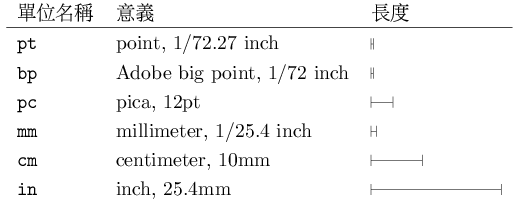
\includegraphics{a-units}
\end{quote}
\end{htmlonly}

�o�̭n�`�N���O \TeX/\LaTeX\ �t�Τ��ҿת��I�]point�^\index{�I�]point�^}�A�����O�@�몺 printer point\index{printer point}�A�]�N�O $1/72.27$~inch�A���b Adobe ���W�椤�A�Ҧp \textsc{PostScript}\index{PostScript@\textsc{PostScript}} �y�������ҿ��I�A�L�O big point\index{big point}�A���� $1/72$~inch�]�p���I�������˥h�F�^�A�|��@�몺 print point �y�L�j�@�I�I�C

\subsection{�۹���}
\index{�۹���}
%begin{latexonly}
\begin{quote}
\begin{tabular}{>{\tt}lll}
���W�� & �N�q & ���� \\
\hline
em & �����b�ϥΦr���r�� M ���e�� & \drawwidth{1em} \\
ex & �����b�ϥΦr���r�� x ������ & \drawwidth{1ex} \\
\end{tabular}
\end{quote}
%end{latexonly}

\begin{htmlonly}
\begin{quote}
\includegraphics{r-units}
\end{quote}
\end{htmlonly}

�b \TeX\ ���Y�ҿת� em\index{em}�A���A��T�Ө��O���b Knuth �б³]�p�� Computer Modern �r�����Y�� em-dash\index{em-dash} ���e�סA�ѩ�r�� M ��ڤW�O�]�b�r���W�ҿת� em-square ���Q��椤�A�� em �ҫ����e�׬O���o�� em-square\index{em-square} ���e�סA���r�� M �����ä��������o�� em-square�A�]���o�˴N�|�y���t���F�C�ҥH�H�r�� M ���e�רӻ������ܮe�����øq�C\LaTeX\ ���ӫ��O \verb|\quad|\index{quad@\verb=\quad=} �o�N�O���ͤ@�ӥ��T em ���e�ת��ťաA�ҥH�b Knuth �бª� \textit{The \TeX{}book} ���A���� em �N�������L�O�@�� `quad' ���e�סC


\section{�����j�p}
\label{sec:layout}\index{�����j�p}

�ڭ̹��ү౱��@��i�Ȫ��d�򳣥i�H�٬������C���M�A�ڭ̪�����]body�^\index{����]body�^}�ä��O������i�Ȫ��d��A�W�U���k���|�d���@�w���ťաC�p�ɭԦb�ůȤW�m�߼g�򵧡A�Ѥ@�������|�n�ڭ̯d�u�Ѧa�v�A�o�N�O������|�P���ťաA���F��ı�W���z�ѡA�j���]�O�H�ͪ����z�a�H:-)

�b�s��W�A�]���H�٤���]body�^���������u���ߡv�Ρu���f�v\index{����}\index{���f}�A�|�P���ťճ����A�h�٬��u����v\index{����}�C��}���ߡB���䪺�]�p�A�N�٤����u�X��v\index{�X��}�A�Ҧp�A�H�I���ϧG����i�ȷ����O�I�������X�A�H�o�ӭI���ϦӨ��A�N�L�ҿת���F�C���o�b \LaTeX\ �q�`�O���|���o�ر��p�X�{�A���D�S�N�h���w����M�ȱi�j�p�P�˽d��C

���M�A�b����H�~���ťաA�]�ëD���O�ťաA�L�]�t�F�����]footer�^\index{�����]footer�^}�A���ܡ]header�^\index{���ܡ]header�^}������]marginal note�^\index{���}\index{marginal note}�������A�O�����󭶼ơB���ѵ���T�C

\subsection{�����ϸ�}
\label{subsec:layout}

\begin{quote}
\begin{center}
\includegraphics{layout-r}
\end{center}
\end{quote}

�o�̩ҿת��ȱi�j�p\index{�ȱi�j�p}�A�����O {\tt paperwidth}\index{paperwidth} �M {\tt paperheight}\index{paperheight} �ҳ򦨪��d��A�ëD��ڤW��W���쪺�ȱi�j�p�A��ڦb��W���ȱi�q�`�|���j��ڭ̳o�̪��ҿׯȱi�A�ҥH�A�����C�L�ɡA�ٻݰ��L�թκI���~�|�O�u�����o�̩ҿת��ȱi�j�p�]�����j�p\index{�����j�p}�^�C

�o�O 10pt ����j�p�A�p�G�����w�ȱi���ܡA\LaTeX\ �w�]�|�ϥά��� {\tt letterpaper}\index{letterpaper} ���j�p�A�p�n�ϥμڡB�馡�� {\tt a4paper}\index{a4paper} ���ܡA�n�t����w�C�ڭ̥i�H�y�L�ݤ@�U \LaTeX\ �w�]�O�p��w�ƪ����Ŷ����C�䤤 Header�]���ܡ^�BFooter�]�����^��������Ŷ��O���t�A�b���� Body ���Y���A�o�̬O�u�O�歱���ϡA�p�G�O�������ܡA�����ƭ��M�_�ƭ�������O�n���k�ﴫ���A�]�N�O���o�ӹϬO�_�ƭ��A���ƭ����ܡA����O�b����C

�o�̧ڭ̨Ӭݤ@�U�o�ǭȩҥN�����N�q�G

\begin{quote}
\begin{tabular}{ll}
���O�]�ȡ^& �N�q \\
\hline
\verb=\paperwidth=	& �ȱi���e�� \\
\verb=\paperheight=	& �ȱi������ \\
\verb=\textwidth=	& ����]body�^���e�� \\
\verb=\textheight=	& ����]body�^������ \\
\verb=\headheight=	& ���ܡ]header�^���� \\
\verb=\headsep=		& ���ܻP���嶡���Z�� \\
\verb=\footskip=	& ���婳�ܭ��������Z�� \\
\verb=\topmargin=	& ���ܤW�誺�ť� \\
\verb=\marginparwidth=	& ������e�� \\
\verb=\marginparsep=	& ����P���媺�Z�� \\
\verb=\marginparpush=	& ��������Z \\
\verb=\oddsidemargin=	& ���奪�䪺�ťդj�p \\
\verb=\hoffset=		& �L�ժ����b��گȱi�����k��m \\
\verb=\voffset=		& �L�ժ����b��گȱi���W�U��m \\
\index{paperwidth@\verb=\paperwidth=}\index{paperheight@\verb=\paperheight=}%
\index{textwidth@\verb=\textwidth=}\index{textheight@\verb=\textheight=}%
\index{headheight@\verb=\headheight=}\index{headsep@\verb=\headsep=}%
\index{footskip@\verb=\footskip=}\index{topmargin@\verb=\topmargin=}%
\index{marginparwidth@\verb=\marginparwidth=}\index{marginparsep@\verb=\marginparsep=}%
\index{marginparpush@\verb=\marginparpush=}%
\index{oddsidemargin@\verb=\oddsidemargin=}%
\index{hoffset@\verb=\hoffset=}\index{voffset@\verb=\voffset=}%
\end{tabular}
\end{quote}

\verb|\hoffset| �� \verb|\voffset| �N�O�b�վ㪩���b��گȱi�W�����T��m�A�o�˦L�X�Ӫ��ɭԤ~�|�b��گȱi�������C

�Y���F�ܡH�o�ܥ��`�A�]�� \LaTeX\ �������]�w��챵IJ���H�ӻ��A�O�c�W�L�����x���B�·СA�]���o�̤��h�ͥL���]�w�A��}�l��b�S�����n��ɶ���b�o�Ӧa��C�p�G��ڷQ�վ㪩���A��ij�ϥ� {\sf geometry}\index{geometry@\textsf{geometry}} package�C�|�ӨҤl�A�Q���U��t�O 2cm �N�n�A���u�n�b preamble\index{preamble} �ϳ]�w�G

\begin{quote}
\begin{verbatim}
\usepackage[margin=2cm]{geometry}
\end{verbatim}
\end{quote}

�N�i�H�F�A�p�G�H 12pt �j�p���r�A{\tt a4paper} �ȱi�j�p���]�w���ܡA�H����Ө��A�j���O�C�� 40 �Ӥ���r�A�o�O���媺�e�סC�i�H�����Φۦ�վ� {\tt margin}\index{margin} ���ȴN��F�C�ڭ̫ܧƱ�A�U�@���� \LaTeX\ ���o�譱���ﵽ�A�H��K�ϥΪ̳]�w�C
%���T�B�ԲӪ��]�w��k�A�ڭ̯d��᭱�������y���ѮɦA�ӽ͡A�o�˴N���P�v�T�ڭ̾Dzߪ����`�i�סC

\subsection{�ȱi�j�p}

\begin{quote}
\begin{tabular}{>{\tt}ll>{\tt }ll}
�ȱi & �j�p & �ȱi & �j�p\\
\hline
a4paper        & 21x29.7cm & letterpaper    & 8.5x11in \\
a5paper        & 14.8x21cm & legalpaper     & 8.5x14in \\
b5paper        & 17.6x25cm & executivepaper & 7.25x10.5in \\
\end{tabular}
\end{quote}

�ܩ�p����w�ȱi�j�p�A�o�̥�²�满���@�U�o�g�峹���]�w�A�ͨ� \LaTeX\ ����Z���O�ɷ|�A�Բӻ����C

\begin{quote}
\begin{verbatim}
% ���媺�]���O�]�w
\documentclass[12pt,a4paper]{report}
\end{verbatim}
\end{quote}

�ҥH�A�o�g�峹�ϥΪ��O {\tt a4paper}�A����r�����j�p�O 12pt�C��A�����ѼƬO�ﶵ�A�i�H�ٲ��A�p�G�ٲ����ܡA�w�]�ȴN�O 10pt/{\tt letterpaper}�C

\section{�վ��V�Ŷ�}

�o�̪���V�Ŷ��A�Ҧp \verb|~|\index{~@\verb=~=} �o��r�����`�ťաA�� \verb|\quad| �o�� em\index{em} �e�תťաA���O�b�վ��V���ťաC���p�G�O�n��j�B�Χ�p���ťծɸӦp��վ�O�H���U�ڭ̴N�Ӭݬ� \LaTeX\ �������򱱨���O�i�H�B�ΡG

\subsection{�վ��V�Ŷ������O}

\begin{quote}
\begin{tabular}{ll}
���O & �N�q \\
\hline
\verb=\hspace{���}= & �V�k�ťX�Y�ӫ׶q��쪺�ťաA�p�G�O�t�ơA�h�O�V�� \\
\verb=\hfill=        & �����k��Ǫ���r�������X�i�ܤ@�Ӧ�e���� \\
\verb=\quad=         & �ťX�@�� em ��쪺�ť� \\
\verb=\qquad=        & �ťX�G�� em ��쪺�ť� \\
\verb=\thinspace=    & �ťX $1/12$ �� em ��쪺�ť� \\
\verb=\enspace=      & �ťX $1/2$ �� em ��쪺�ť� \\
\verb=\dotfill=      & �@�ΩM \verb|\hfill| �ۦP�A�u�O�ť��ܦ��I \\
\verb=\hrulefill=    & �@�ΩM \verb|\hfill| �ۦP�A�u�O�ť��ܦ��@��u \\
\verb=\centering=    & �����O�H�᪺��r�N�|�~���ƦC�A���k�u�N������ \\
\verb=\raggedright=  & �����O�H�᪺��r�N�|�~���ƦC�A�k�u�N������ \\
\verb=\raggedleft=   & �����O�H�᪺��r�N�|�~�k�ƦC�A���u�N������ \\
\verb=\centerline{}= & �N�j�A��������r�~���ƦC
\end{tabular}
\end{quote}
\index{hspace@\verb=\hspace=}\index{hfill@\verb=\hfill=}%
\index{quad@\verb=\quad=}\index{qquad@\verb=\qquad=}%
\index{thinspace@\verb=\thinspace=}\index{enspace@\verb=\enspace=}%
\index{dotfill@\verb=\dotfill=}\index{hrulefill@\verb=\hrulefill=}%
\index{centering@\verb=\centering=}\index{raggedright@\verb=\raggedright=}%
\index{raggedleft@\verb=\raggedleft=}\index{centerline@\verb=\centerline{}=}

�@�檺�歺�ϥ� \verb|\hspace{���}| �ɱN�|���ġA�o�ɥi�H�[�ӬP���A�Ҧp \verb|\hspace*{3em}|�C

�b�ϥ� \verb|\centerline{}| �����X�A���u��y�ܤ�K�A�]���L���|�v�T�H�U����r�A���L�]���|���A�Ʀܥ[�J����Ÿ��]�L�ġC�ҥH�p�G��y���׶W�L�@�檺��e�A�L�|�W�X��ɡA�ƦܴN��������r�N�ݤ���F�C

�䤤 \verb|\thinspace| �S�i�H�ϥ�²�ƪ� \verb|\,| �ӥN���A�D�n�O�Φb�޸����S���޸������ΡA�q�`�o�ر��ΡA��޸������n���Ӷ��j�A�H�K�Ϥ��A�Ҧp�G

\begin{quote}
\begin{verbatim}
``\,`Superman', he said.''
\end{verbatim}
\end{quote}

���{�X�ӷ|�O�G

%begin{latexonly}
``\,`Superman', he said.''
%end{latexonly}

\begin{htmlonly}
\begin{quote}
\includegraphics{superman}
\end{quote}
\end{htmlonly}

�o�ˤ~��Ϥ��X���P�޸��A�_�h�|�ܦ��@�ӳs�T�� grave accent\index{grave accent} ���޸��C�Ъ`�N�A�ѩ�o�ӫ��O�O�ѫD�r���Ÿ��c���A�ҥH�A�L���@�νd��b�J��Ÿ�������N�����F�A�᭱�����ťթΥH�j�A���ӭ����@�νd��A�N�n��������L�� \verb|\@| �@�˪����ΡC

\subsection{�վ��V�Ŷ�������}

\begin{quote}
\begin{tabular}{ll}
\verb|\begin{center}...\end{center}| & ���o�����Ҥ������e�m�� \\
\verb|\begin{flushleft}...\end{flushleft}| & ���o�����Ҥ������e�a�� \\
\verb|\begin{flushright}...\end{flushright}| & ���o�����Ҥ������e�a�k \\
\verb|\begin{raggedright}...\end{raggedright}| & ���o�����Ҥ������e�a���A�k�u�N������ \\
\verb|\begin{raggedleft}...\end{raggedleft}| & ���o�����Ҥ������e�a�k�A���u�N������ \\
\end{tabular}
\end{quote}
\index{center@\texttt{center}}\index{flushleft@\texttt{flushleft}}%
\index{flushright@\texttt{flushright}}\index{raggedright@\texttt{raggedright}}%
\index{raggedleft@\texttt{raggedleft}}

�i�J���ҡA�M�W�@�`���쪺���O�A��̦����򤣦P�O�H�̤j�����P�O�A�o�i�H��K�����w�@�ӽd�򪺤�y���L�@�ΡA�Ӥ��|�v�T���ҥH�~����y�C�䦸�A�i�J���ҡA�a�ϩM�W�U��s�b�@�_�A�S���ťX�ťզ�A�L�]�|�۰ʪ��b�W�B�U��ťX�Ӫťզ�X�ӡA�ϥΫ��O���ܫh���|�C

�x�I�o�̫��S���� {\tt raggedright} �� {\tt raggedleft}�H��ӥL�]�O�i�H�����ҨӨϥΡC�ѩ�o��ӫ��O�|�ϥH�U�����e�����B�k�u�������A�]���ϥΤW�n�D�`�p�ߡA���D���ӴN�Q�����媺���B�k�u�������A�_�h�A�̦n�O�ϥΦ��d�򭭨�覡�C���M�A�p�G�o��ӫ��O�O�Φb�Y�Ө�L���ҽd�򤺡A�L���@�Τ]�N�ȭ���o�����Ҥ��A���|�v�T�o�����ҥ~����y�C

\subsection{�ޤ�����}
\index{�ޤ�����}

�ޤ�q�`�N�O�ޥΥL�H����y�A�b�ޤ媺�q���A��dz��|�X�{���Y�����ΡA�H�K�M����۰Ϲj�A�o�]�O�@�تŶ����t�m�A�i�W�[�峹����Ū�ʡC�b \LaTeX\ ���Y���T�ؤޤ����ҡG{\tt quote}, {\tt quotation}, {\tt verse}�C�o�T�̬ݰ_�ӫܹ��A�����ǷL���t���C

\begin{quote}
\begin{tabular}{>{\tt }lll}
���� & �A�ήɾ� & �S�� \\
\hline
quote & ���u���u�ޤ� & �C�Ӭq���Ĥ@�椣���Y \\
quotation & �h�Ӭq�������ޤ� & �C�Ӭq���Ĥ@��|���Y \\
verse & �ֺq�B���ޤ� & �C�Ӭq�����Ĥ@�椣���Y�A���ĤG��_�|���Y \\
\end{tabular}
\end{quote}
\index{quote@\texttt{quote}}\index{quotation@\texttt{quotation}}%
\index{verse@\texttt{verse}}

�b {\tt verse} �����ΡA�q�`�|�ϥ� \verb=\\=\index{\\@\verb=\\=} �Ӵ���H�K����C�@�檺�e�סC�ӥB�q�����Z\index{�q�����Z}�N�����~�b�]�w���v�T�A�䤤 {\tt quote} �M {\tt verse} ���ҷ|�w���J�A�����q�����Z�A�� {\tt quotation} ���ҫh���|�C

���U�ڭ̨Ӭݬݽվ��V�Ŷ����@�Ӻ�X��ҡG

\begin{quote}
\begin{verbatim}
% example11.tex
\documentclass{article}
\usepackage{CJK}
\begin{document}
\begin{CJK}{Bg5}{hwmm}
\section{hspace}
\hspace*{2em}�o�O�@�Ӿ�V�Ŷ��վ㪺���աC\\
�o�O�@��\hspace{2em}��V�Ŷ��վ㪺���աC\\
�o�O�@�� \hspace{2em} ��V�Ŷ��վ㪺���աC
\section{hfill}
�o�O�@��\hfill{}��V�Ŷ��վ㪺���աC
\section{quad}
�o�O�@��\quad{}��V�Ŷ��վ㪺���աC\\
�o�O�@�� \quad{} ��V�Ŷ��վ㪺���աC\\
�o�O�@��\qquad{}��V�Ŷ��վ㪺���աC
\section{dotfill}
�o�O�@��\dotfill{}��V�Ŷ��վ㪺���աC\\
�o�O�@�� \dotfill{} ��V�Ŷ��վ㪺���աC
\section{hrulefill}
�o�O�@��\hrulefill{}��V�Ŷ��վ㪺���աC
\section{center}
\begin{center}
�o�O�@�Ӿ�V�Ŷ��վ㪺���աC
\end{center}
\section{flushleft}
\begin{flushleft}
�o�O�@�Ӿ�V�Ŷ��վ㪺���աC
\end{flushleft}
\section{flushright}
\begin{flushright}
�o�O�@�Ӿ�V�Ŷ��վ㪺���աC
\end{flushright}
\section{quote}
�o�O�`���ۥ���J�����`���G�ơG
\begin{quote}
An antwent to the bank of a river to quench its thirst, and
being carried away by the rush of the stream, was on the
point of drowning.

A Dove sitting on a tree overhanging the water plucked a
leaf and let it fall into the stream close to her. The Ant
climbed onto it and floated in safety to the bank.
\end{quote}
\section{quotation}
�o�O�`���ۥ���J�����`���G�ơG
\begin{quotation}
An antwent to the bank of a river to quench its thirst, and
being carried away by the rush of the stream, was on the
point of drowning.

A Dove sitting on a tree overhanging the water plucked a
leaf and let it fall into the stream close to her. The Ant
climbed onto it and floated in safety to the bank.
\end{quotation}
\section{verse}
�o�O�`���ۥ���J�����`���G�ơA�o�O�`���ۥ���J�����`���G�ơA%
�o�O�`���ۥ���J�����`���G�ơA�o�O�`���ۥ���J�����`���G�ơG
\begin{verse}
An antwent to the bank of a river to quench its thirst, and
being carried away by the rush of the stream, was on the
point of drowning.

A Dove sitting on a tree overhanging the water plucked a
leaf and let it fall into the stream close to her. The Ant
climbed onto it and floated in safety to the bank.
\end{verse}
\section{centering}
\centering
�o�O�@�Ӿ�V�Ŷ��վ㪺���աC\\ % �o�̭n����A�_�h�|�O \raggedright ���@��
\raggedright
\section{centerline}
\centerline{�o�O�@�Ӿ�V�Ŷ��վ㪺���աC}
\section{raggedright}
\raggedright
�o�O�@�Ӿ�V�Ŷ��վ㪺���աC
\section{raggedleft}
\raggedleft
�o�O�@�Ӿ�V�Ŷ��վ㪺���աC
\end{CJK}
\end{document}
\end{verbatim}
\end{quote}

�sĶ�n�����G�p�U�G

\begin{quote}
\url{http://edt1023.sayya.org/tex/latex123/example11.tex}\\
\url{http://edt1023.sayya.org/tex/latex123/example11.pdf}
\end{quote}

�n�`�N�O���O�e�᪺�ťաA�� \verb|\hspace|, \verb|\dotfill|, \verb|\hrulell| �o�����O�A���O�e��ťճ��|��i�h���C\verb|\quad|, \verb|\qquad| �o�����O�A�h�᭱���ťդ]�O�|��J���C�t�~�A�ѨҤl���i�H�ݥX�ӡA�@�� em\index{em} ���e�סA�j���O�@�Ӥ���r���e�סA�ҥH�A�ڭ̹w�]�ϥ� 10pt ���r�A�o�� em �e�״N�۷��� 10pt ���e�סA�ҥH�A�ڭ̦b�Ĥ@�洡�J�F 2em �e�ת��ťաA�]�N�n���O���Y�F��Ӥ���r�@�ˡC

\section{�վ��a�V�Ŷ�}

\begin{quote}
\begin{tabular}{ll}
\verb=\vspace{���}= & �V�U�ťX�Y�ӳ�쪺�ťա]��^�A�t�ƫh�O�V�W \\
\verb=\bigskip=     & ���� 12pt�]11--12pt�^�������ťա]��^ \\
\verb=\medskip=     & ���� 6pt�]5--7pt�^�������ťա]��^\\
\verb=\smallskip=   & ���� 3pt�]2--4pt�^�������ťա]��^\\
\verb=\vfill=       & �M \verb|\hfill| �����A�@�άO�N�Y�q���V�W���A�Ω��U�� \\
\verb=\parskip=���= & �վ����C�Ӭq�������Z�����Y�ӳ��
\index{vspace@\verb=\vspace=}\index{bigskip@\verb=\bigskip=}%
\index{medskip@\verb=\smallskip=}\index{vfill@\verb=\vfill=}%
\index{parskip@\verb=\parskip=}
\end{tabular}
\end{quote}

�䤤�� \verb|\bigskip, \medskip, \smallskip| �ëD�T�w���A�L�̷|���W�U��ߵ����ݭn�۰ʰ��L�աA�H�F��@�㭶���@�P���Ŷ��t�m�C\verb|\vspace| �p�G�O�X�{�b�@�����Ĥ@��γ̫�@��ɡA�N�|���h�@�ΡA�o�ɥi�H�[�ӬP���A\verb=\vspace*{���}=\index{vspace@\verb=\vspace*=}�C

���F�����������@�P��\index{�����@�P��}�A�ϥ��a�V�Ŷ��վ㪺���O�ɭn�S�O�d�N�A�Ҧp���`���D�W�U���Ŷ��B�U�q�������Ŷ��A�i�J���ҫe��ҪťX���Ŷ��A�o�����@�өT�w�ȡA\LaTeX\ �|�۰ʥh�վ�A�����ѨϥΪ̦ۦ�ʤ�A���D�O�ʭ��o�س�W���C�ҥH�A�ϥ��a�V�Ŷ��վ���O�ɡA�n�D�`�`�N���骺�@�P�ʡA�o�]�O�ƪ��W���@�ӫܭ��n����h�C

�o���|�o�g�峹�������ʭ�\index{�����ʭ�}���ҨӺ�X�����A��B�a�V�Ŷ����B�ΡC�ٰO�o�� \ref{sec:titlepage} �`�� title page\index{title page} �����O�ܡH���ڭ̤]�i�H�ۦ�]�p�@�ӿW�ߪ������ʭ��A�ϥΪ��O \LaTeX\ ������ {\tt titlepage}\index{titlepage@\texttt{titlepage}} ���ҡC�o�̪����ɤޥάO�ڭ��٨S���Dzߨ쪺�A�S���Y�A�u�n�j��h����N��F�C

\begin{quote}
\begin{verbatim}
% example12.tex
\documentclass[12pt,a4paper]{report}
\usepackage{CJK}     % �ޤJ�һݭn�� packages
\usepackage{graphicx}
\begin{document}
\begin{CJK}{Bg5}{hwmm}
\begin{titlepage}    % �ϥ� titlepage ����
\vspace*{5ex}
  \begin{flushright} % �j���D�a�k
    \Huge\textbf{�j�a�Ӿ� \LaTeX}
  \end{flushright}
  \rule{\textwidth}{.256ex}
  \begin{flushleft}  % �������X����a���A�M�j���D�����H�@��u�j�}
    Version 0.1 draft\\
    \today
  \end{flushleft}    % ���ɦ�󤤥�����
  \vspace{8ex}       % �ťX 8ex �������Ŷ�
  \hspace{2em}\includegraphics[scale=.75]{cover2.1} % �ޤJ���ɡA�ñN�o��
  \vspace{8ex}                                      % ���ɾ�V�k�� 2em
  \begin{flushright} % �@�̸�T�a�k
    By Edward G.J. Lee ���G��\\
    Email�G\texttt{edt1023@info.sayya.org}
  \end{flushright}
\end{titlepage}
\end{CJK}
\end{document}
\end{verbatim}
\end{quote}

�ѩ�t�X���������D�A�䤤���@�Ǽƾڦ���ʡA�ӥB�]�ٲ��F�@�ǧڭ��٨S���Dzߨ쪺 packages�A���j���c�h�M��l��Z�@�ˡC�ҥH�A�M�o�g�峹�� PDF �榡����|�o�{�A�j���D���r��p�F�@�I�A�ӥB�S���C��A�]�S���W�s��\index{�W�s��}�C

�ϥ� {\tt titlepage}\index{titlepage@\texttt{titlepage}} ���ҫ�A�b {\tt report/book}\index{report@\texttt{report}}\index{book@\texttt{book}} ��Z�L�|�ۦ��@�S�����ƪ���W���A�b {\tt article}\index{article@\texttt{article}} ���O�A�]���|�M����s���A�ҥH�A�b�ﶵ�������n�h�[�@�� {\tt titlepage}\index{titlepage} ���ﶵ�C�t�~�A�b {\tt titlepage} ���Y�N����A�ϥ� \verb|\title|\index{title@\verb=\title=}, \verb=\author=\index{author@\verb=\author=} ���O�F�A�b���媺�a��]�����A�U \verb=\maketitle=\index{maketitle@\verb=\maketitle=} ���O�C

�sĶ�n���Ҥl�p�U�G

\begin{quote}
\url{http://edt1023.sayya.org/tex/latex123/example12.tex}\\
\url{http://edt1023.sayya.org/tex/latex123/example12.pdf}
\end{quote}

�o�̭n�S�O�������O�A�ޤJ���ɭn�ϥ� \textsf{graphicx}\index{graphicx@\textsf{graphicx}} package�]�o�O�̱`�Ϊ��A�]����L����k�ӤޥΡ^�A�ޤJ�����O�O \verb=\includegraphics=\index{includegraphics@\verb=\includegraphics=}�A�o�ӧڭ̷|�b�� \ref{ch:graphic} ���|�Q�סA�b�o�̧ڭ̧�����Y�p������Ϫ� {\tt 75\%}�A�_�h��ӫʭ��|�W�X�@���C�o�ӹ��ɬO�� \MP\index{metapost@\MP} �ɮשҽsĶ�ӨӪ��A�L�O�@�� eps ����\index{eps ����}�]²�檺���A�O�t����ɼƾڥh�������n�P��ťժ� ps ��\index{ps ��}�A��K�ޤJ�ο�X�ܤ�Z���^�A�sĶ����k�p�U�G

\begin{quote}
\begin{verbatim}
mpost cover2.mp
\end{verbatim}
\end{quote}

�o�˴N�|���� {\tt cover2.1} �o�� eps ���ɡA�o�˴N�i�H�����ޤJ�F�C�L����l�X�� eps ���ɦb�G

\begin{quote}
\url{http://edt1023.sayya.org/tex/latex123/cover2.mp}\\
\url{http://edt1023.sayya.org/tex/latex123/cover2.1}
\end{quote}


\section{���C����}

���C����\index{���C����}�]�O�ݩ�@�تŶ�������A�L��@�Ǥ�r���@�w���覡�ӱƦC�A���C���Ҥ��@�ǰ_�Y���Ÿ��B��Ʀr�Φr��A�ڭ̺٤������ؼ��ҡ]item label�^\index{���ؼ��ҡ]item label�^}�A�Q�γo�Ǥ��@�˪��ƦC��m�Τ��@�˪����ؼ��Ұ_�Y�ӱԭz��y�A�N�i�H�F����ت��@�ΡC�o�O�H���`���j�H�~�A�۷��`�������e�@�ؤF�M����k�A��ij�h�h�Q�ΡC�Фd�U�O�o�A���Ҥ��٥i�H�����ҡA�ӥB�H�U�T�ت����C�覡�i�H�V�X��e�ϥΡC

\subsection{���ئ����C���ҡ]itemize�^}
\index{���ئ����C���ҡ]itemize�^}

�o�O�H�Ÿ��Ӱ_�Y���ت��@�ر��C�覡�C�Ҧp�G

\begin{quote}
\begin{verbatim}
\begin{itemize}
\item �Ĥ@�j���A�o�̬O�Ĥ@�j���C
\item �ĤG�j���A�o�̬O�ĤG�j���C
 \begin{itemize}
 \item �Ĥ@�p���A�o�̬O�Ĥ@�p���C
 \item �ĤG�p���A�o�̬O�ĤG�p���C
 \end{itemize}
\item �ĤT�j���A�o�̬O�ĤT�j���C
\item �ĥ|�j���A�o�̬O�ĥ|�j���C
\end{itemize}
\end{verbatim}
\end{quote}

�ƪ��X�ӷ|�ܦ��G

%begin{latexonly}
\begin{quote}
\begin{itemize}
\item �Ĥ@�j���A�o�̬O�Ĥ@�j���C
\item �ĤG�j���A�o�̬O�ĤG�j���C
  \begin{itemize}
  \item �Ĥ@�p���A�o�̬O�Ĥ@�p���C
  \item �ĤG�p���A�o�̬O�ĤG�p���C
  \end{itemize}
\item �ĤT�j���A�o�̬O�ĤT�j���C
\item �ĥ|�j���A�o�̬O�ĥ|�j���C
\end{itemize}
\end{quote}
%end{latexonly}

\begin{htmlonly}
\begin{quote}
\includegraphics{itemize}
\end{quote}
\end{htmlonly}

\subsection{�C�|�����C���ҡ]enumerate�^}
\label{subsec:enume}\index{�C�|�����C���ҡ]enumerate�^}

�o�O�H�ƥئr�Φr����ù���Ʀr�Ӱ_�Y���ت����C�覡�C�P�˪��Ҥl�A�令 {\tt enumerate} ���ܡA�|�ƪ����G

%begin{latexonly}
\begin{quote}
\begin{enumerate}
\item �Ĥ@�j���A�o�̬O�Ĥ@�j���C
\item �ĤG�j���A�o�̬O�ĤG�j���C
  \begin{enumerate}
  \item �Ĥ@�p���A�o�̬O�Ĥ@�p���C
  \item �ĤG�p���A�o�̬O�ĤG�p���C
  \end{enumerate}
\item �ĤT�j���A�o�̬O�ĤT�j���C
\item �ĥ|�j���A�o�̬O�ĥ|�j���C
\end{enumerate}
\end{quote}
%end{latexonly}

\begin{htmlonly}
\begin{quote}
\includegraphics{enumerate}
\end{quote}
\end{htmlonly}

\subsection{�ԭz�����C���ҡ]description�^}
\index{�ԭz�����C���ҡ]description�^}

�o�O�H�@��²�u��r�ԭz�Ӱ_�Y���ت����C�覡�C�A��L�令 {\tt description} ���ܡA�L�O�H�����r�Ӱ_�Y���ت��A�o�Ǥ�r�n�Τ�A���A���C

\begin{quote}
\begin{verbatim}
\begin{description}
\item[�Ĥ@�j��] �o�̬O�Ĥ@�j���C
\item[�ĤG�j��] �o�̬O�ĤG�j���C
  \begin{description}
  \item[�Ĥ@�p��] �o�̬O�Ĥ@�p���C
  \item[�ĤG�p��] �o�̬O�ĤG�p���C
  \end{description}
\item[�ĤT�j��] �o�̬O�ĤT�j���C
\item[�ĥ|�j��] �o�̬O�ĥ|�j���C
\end{description}
\end{verbatim}
\end{quote}

�ƪ��X�Ӫ����G�O�G

%begin{latexonly}
\begin{quote}
\begin{description}
\item[�Ĥ@�j��] �o�̬O�Ĥ@�j���C
\item[�ĤG�j��] �o�̬O�ĤG�j���C
  \begin{description}
  \item[�Ĥ@�p��] �o�̬O�Ĥ@�p���C
  \item[�ĤG�p��] �o�̬O�ĤG�p���C
  \end{description}
\item[�ĤT�j��] �o�̬O�ĤT�j���C
\item[�ĥ|�j��] �o�̬O�ĥ|�j���C
\end{description}
\end{quote}
%end{latexonly}

\begin{htmlonly}
\begin{quote}
\includegraphics{description}
\end{quote}
\end{htmlonly}

�n�`�N���O�A���ޭ��@�ت����C���ҡA�C�Ӷ��ء]item�^����r�ԭz�|�۰ʧ��A�o�۷���K�A�ϥΪ̥u�n����C�����c�˧��A�M�ߥ��C�Ӷ��ت����e�N���F�C�ӥB�A�p�G�ϥΤ�A���A���@�Ǧr���B�r��βŸ��A���a�Y���ХܱN�|�O�o�Ǧr���B�r��βŸ��A�p�G�O�C�|�������C�覡�A���򦳤�A�����N���Q�s���A�|�۰ʸ��L�A�s�����ǫh�|�۰ʶ����C

%\section{enumerate �����M��}

%\subsection{���C���Ҥ����Ŷ�����}


\section{�u��}
\index{�u��}

�u�ئb�ƪ��W�����@�w���a��A�]���L�i�H�Ϲj���P���Ŷ��A�]�i�H���Y�dz�������X�ӡC���O�A�L�h���u�ؤ]�O�|���ٻ��ܥD�����n�Ƨ@�ΡA�ϥΤW�i��n�A�i�Ӥ�C�o�̧ڭ̭n�ͪ��O��ª��u�ءA����\index{����}�]�O�u�ت��@�����ΡA�ڭ̱N�|�b�� \ref{ch:graphic} ���A�A�ӽͪ��檺�B�z�C

%�b \LaTeX\ ���u�إi�����T�ءGLR�BRule �� Par�C

%\begin{quote}
%\begin{tabular}
%�u�غ��� & �N�q \\
%\hline
%LR  & left-right�A�u�ؤνu�ؤ������e�ѥ��ܥk \\
%Rule & 
%Par
%\end{tabular}
%\end{quote}

\subsection{���u�]rule�^}
\index{���u�]rule�^}

���u�]�O�ݩ��ت��@�ءA�N�O�@�ӹ������ΡA�u���L�A�L�����μe�]�u���ղӡ^�u���@�I�I�A�ҥH�A�ݰ_�ӴN�@�����u�}�F�C

\begin{quote}
\begin{verbatim}
\rule[�W�U��m(���)]{�e}{��}
\end{verbatim}
\end{quote}

�e�ΰ��������h�������A���ӤW�U��m�O����O�H�o�ӤW�U��m�O�M��u�]baseline�^\index{��u}\index{baseline}�b������A�p�G�S�����w�A���N�O�b��u����m�A�p�G�����w�A�N�̥��t�Ƚվ�M��u���۹��m�A���ȥѰ�u�V�W�վ�A�t�ȫh�Ѱ�u�V�U�վ�C�o�̨Ӭݭӭӹ�ҴN�A�ѤF�G

\begin{quote}
\begin{verbatim}
% example13.tex
\documentclass{article}
\parskip=3pt
\parindent=0pt
\begin{document}
This is a line.       % �e�� 1pt �e 3cm ����u�C
\rule{3cm}{1pt}
\rule[1ex]{3cm}{1pt}
\rule[-1ex]{3cm}{1pt}

\rule{1pt}{3cm}      % �e�� 3cm �e 1pt �����u�C

\rule{3cm}{0pt}TEST. % �� TEST �V�k�� 3cm�C

\rule{2cm}{3cm}      % �e�� 3cm �e 2cm �������ءC

\textcolor{blue}{This is color lines.}
\textcolor{red}{\rule{3cm}{1pt}}        % ���C�⪺�u�ءC
\textcolor{green}{\rule[1ex]{3cm}{1pt}}
\textcolor{blue}{\rule[-1ex]{3cm}{1pt}}
\end{document}
\end{verbatim}
\end{quote}

�sĶ�n���Ҥl�b�G

\begin{quote}
\url{http://edt1023.sayya.org/tex/latex123/example13.tex}\\
\url{http://edt1023.sayya.org/tex/latex123/example13.pdf}
\end{quote}

�ѨҤl���i�H�ݱo�X�ӡA�o�ӵe�u���O�ä��O����a�B��e�u�Ӥw�A�F���B�Ϊ��ܡA�i�H���X�\�h���P���ĪG�A�Ҧp����Ϥ������C

\subsection{��r���u�]underline�^}
\index{��r���u�]underline�^}

���ɭԧڭ̧Ʊ�b�Ѽg��r���P�ɡA�]�b��U�e�u�C\LaTeX\ ���{�������O�i�H�ϥΡA���N�O \verb|\underline{��r}|\index{underline@\verb=\underline=}�A�|�b��r���u�������P�ɵe�W�u���C���M�A�ϥΤW�`�`�|�M�{�b����u�d�V�A�]���ϥήɭn�S�O�d�N��ӭ����W�O�_�w�g�s�b�F�\�h��u�C

\subsection{��ء]box�^}
\index{box}

�o�̥D�n������r��ءAø�ϤW���@��اΦb�� \ref{ch:graphic} ���ɦA�ӰQ�סC�o�@�����}�Y�N�w�ͨ�A��g�峹�O�Ѥ@�ӭӪ� box �Һc�����A�o�̪���ثh�O�@�Ө嫬�� box�A�L���a��A���M�O�M�e���һ��� box �@�ˡA\TeX/\LaTeX\ �|��L�����@�ӳ�@���r���ӳB�z�C

�ڭ̥��Ӭݬݳ�²�檺��ت����O�G

\begin{quote}
\begin{tabular}{ll}
���O & �N�q�Χ@�� \\
\hline
\verb=\frame{��r}= & �N��r���e�H�i������خئ��A��ةM��r���S�����Z \\
\verb=\fbox{��r}=  & �N��r���e�H�i������خئ��A��ةM��r�����@�w���Z \\
\verb=\mbox{��r}=  & �@�ΩM \verb|\fbox| �P�A����ؤ��i��
\end{tabular}
\end{quote}
\index{frame@\verb=\frame=}\index{fbox@\verb=\fbox=}%
\index{mbox@\verb=\mbox=}

�H�W�����O���i�H�Φ���ؤ�r�C

��ؤ]���i�H�վ㪺���O�G

\begin{quote}
\begin{tabular}{ll}
���O & �N�q�Χ@�� \\
\hline
\verb|\framebox[�e��][����覡]{��r}| & �P \verb|\fbox| �P�A���i���w�e�פι���覡 \\
\verb|\makebox[�e��][����覡]{��r}| & �P \verb|\mbox| �P�A���i���w�e�פι���覡
\index{framebox@\verb=\framebox=}\index{makebox@\verb=\makebox=}
\end{tabular}
\end{quote}

�o�̪��e�׫����O��ت��e�סA�����w���ܡA�@�δN�p�P \verb|\fbox| �� \verb|\mbox| �@�ˡA�H�]����Ӥ�r�d�򬰼e�סA�ѩ�ڭ̤��e��������r���e���e�צ��h�֡A�]���e�ת����w�i�H�ϥΤU�C�۹��쪺�覡�G

\begin{quote}
\begin{tabular}{ll}
�e�� & �@�� \\
\hline
\verb|\width| & �o�Ӽe�״N�O \verb|\fbox| ����ɪ���ؼe�� \\
\verb|\height| & �o�O���`��u�ܮس������� \\
\verb|\depth| &  �o�O���`��u�ܮة������� \\
\verb|\totalheight| & �o�O \verb|\height| �M \verb|\depth| ���`�M \\
\end{tabular}
\end{quote}

�Ҧp�A�ڭ̫��w \verb|2\width| �L���N��N�O�H \verb|\fbox| �]������r���e�ɡA���ؼe�ת��G���e�C�ѼƸ��Y������覡�A�i���U�C�X�ءG

\begin{quote}
\begin{tabular}{>{\tt }ll}
����覡 & �@�� \\
\hline
c & center�A��r����ؤ����A�o�O�w�]�� \\
l & flushleft�A��r����إ��� \\
r & ushright�A��r����إk�� \\
s & stretch�A��r�������������ؤ�
\end{tabular}
\end{quote}

�����w���ܡA���M�N�O����ؤ�����m�F�C�ڭ̤]�i�H���w�i����ت��u���ʲӡA�Τ�ةM��r�������j�Z���G

\begin{quote}
\begin{tabular}{ll}
���O & �@�� \\
\hline
\verb|\fboxrule=���| & ���w��ؽu���ʲ� \\
\verb|\fboxsep=���| & ���w��r�M�ؽt�����Z%
\index{fboxrule@\verb=\fboxrule=}\index{fboxsep@\verb=\fboxsep=}%
\end{tabular}
\end{quote}

�Ъ`�N�A�o���|�v�T \verb|\frame{}|�C�p�G�Q�S�O���m���ت���m�A�]�i�H�ϥ� \verb|\raisebox|\index{raisebox@\verb=raisebox=} ���O�G

\begin{quote}
\begin{verbatim}
\raisebox{�W�U��m(���)}[�`��][����]{��r���e}
\end{verbatim}
\end{quote}

�o�̪��W�U��m���N�q�M \verb|\rule| ���O���Y���@�ˡA�u���L�A�o�̪��W�U��m�@�w�n���w�A�S���w�]�ȡA�����w�|�sĶ���~�C�Фd�U�O�o�A��ؤ����M�O�٥i�H����ت��C�ڭ̲{�b�N�Ӭݤ@�Ӻ�X����ҡG

\begin{quote}
\begin{verbatim}
% example14.tex
\documentclass{article}
\parskip=3ex
\parindent=0pt
\begin{document}
\frame{This is frame.}
\mbox{This is mbox.}
\fbox{This is fbox.}

\framebox{This is a framebox with no argumant.}

\framebox[1.5\width]{This is a framebox.}

\framebox[1.5\width][l]{This is a framebox with \texttt{l}.}

\framebox[1.5\width][r]{This is a framebox with \texttt{r}.}

\framebox[1.5\width][s]{This is a framebox with \texttt{s}.}

This is baseline.
\raisebox{3ex}[5\height]{This is a raisebox which lift 3ex.}

This is baseline.
\fbox{\raisebox{-3ex}[5\height]{This is a raisebox which lift $-$3ex.}}

\fboxrule=1.5pt
\fboxsep=8pt
\framebox[1.5\width][s]{This is a framebox with \texttt{s}.}
\end{document}
\end{verbatim}
\end{quote}

�o���L�ݦh�[�����A�sĶ�n���Ҥl�b�G

\begin{quote}
\url{http://edt1023.sayya.org/tex/latex123/example14.tex}\\
\url{http://edt1023.sayya.org/tex/latex123/example14.pdf}
\end{quote}

\subsection{�q�����}
\index{�q�����}

�t�~�A�]���Ω�q����r����ءA�i�H����Y�Ӭq���X�{�b�Y�S�w���Ŷ��B��m�C�ڭ̱`�`��o�ئw�ƺ٬��g�A�����A�⪩�����e�m��@�Ӥ��i������ط����A���M�A�o�Ӥ�ةM�@�몺 box�A�Ҧp�r���A���M�B��P�˪��a��A\LaTeX\ �|��L�����@�Ӧr�����ӳB�z�C

\begin{quote}
\begin{verbatim}
\parbox[����覡][����][�����m]{�e��}{��r���e}

\begin{minipage}[����覡][����][�����m]{�e��}
  �q�����e
\end{minipage}
\end{verbatim}
\end{quote}
\index{parbox@\verb=parbox=}\index{minipage@\texttt{minipage}}

�o�̪��Ĥ@�ӿ�ܩʰѼơu����覡�v�G

\begin{quote}
\begin{tabular}{>{\tt }ll}
t & top�A�q����ت��W�u����@�檺��u \\
b & bottom�A�q����ت��U�u����@�檺��u \\
c & center�A�q����ت���������@�檺��u�A�o�O�w�] \\
\end{tabular}
\end{quote}

\verb|\parbox| ���O�q�`�Ω���u����r���e�A�p�G�O�������q���A���ϥ� {\tt minipage} ���ҷ|�����K�C�o�Ǭq����ةM�W���ҽͨ쪺�@�Ǥ�س̤j�����P�O�A�q����إ��N�O�Ψӱƪ��p�q����y�A�]���L�|�M�@�륿�`�峹�q���@�˪��B�z�A�Ҧp�L�|�۰��_��A�I��ťզ�]�|�_�s�q���A���U�q���w�]�O���Y�ƪ��A�ӥB�A�b�w�ƤW�|��@�몺�q�����A�@����t�����Z�|�Y� 0pt�C

���פ��h���w���ܡA���N�O�H��Ӫ����g�_��B�z��A��Ӥ�r�q���ҧΦ������סC�ܩ󤺤��m�����]�O \texttt{t, b, c} �o�ǡA�N��O��r�q���b��ؤ����W�U��m�A���M�A�o�n�����w��ذ��׮ɤ~�|���N�q�A�]���A�u�����m�v�M�u���סv�O�n�P�ɫ��w���A�n�D�`�`�N���O�A�p�G���w�F���סA���S�����w�����m�A�h�w�]�O����e���ϥΪ��u����覡�v�ҫ��w���ѼơC

�o�ǰѼƪ��ϥη|���ǷнơA���o�O�u�ʩұa�Ӫ��u���n���c�v�A�����h���O�A�u���b�Ĥ@����IJ�ɧ�L�d�M���N���F�A��ڭn�Ψ�ɦA�Ӭd�L���ԲӰѼơA�`�Ϊ����O�B���ҡA�j���h�d�X���N�۵M�ӵM���O�_�ӤF�C


% ``�j�a�Ӿ� LaTeX'' LaTeX ��Z class.tex
% Copyright (c) 2004  Edward G.J. Lee <edt1023@info.sayya.org>
%
% �b���H�� GNU Free Documentation License 1.2 �ΥH�᪺�����W�d���U�A
% ���\�����B���G�έק�C���쪩�v�B���v�n�����o�����C
%
% �����G�����A�t�� fdl.tex�A���e�� GNU FDL ���W�d���C�p�G�򥢡A�i��
% http://www.gnu.org ���o�A�μg�H�ܦۥѳn�����|(Free Software Fundation)
% �����C
% 9 Temple Place - Suite 330, Boston, MA 02111-1307, USA.
%
% $Id: class.tex,v 1.14 2004/03/06 17:17:55 edt1023 Exp $
%
\chapter{\LaTeX\ ���зǤ�Z���O}
\label{ch:class}\index{��Z���O}

�o���D�n�O�b���� \LaTeX\ ��Z�����O�]document class\index{document class}�^\footnote{�o�b�ª������٬� style�A�o��ӵ��N�q�W�t���h�A�o�dz��O \TeX\ �����X�Ӫ������w�q�A�M���Ψөw�q�峹���j���c�A�H�K²�ƨϥΤW�Τ�Z�����e�C}�A�o�O \LaTeX\ �W�d��Z���鵲�c����k�C�ϥ� class ���ηN�A�N�O�⪩�����c�B�z�M��ڤ�Z���}�A�o�˪��̤j�n�B�N�O������g�峹�ƪ����c�W���@�P�ʡA�]�Ϥ�Z���e��M�n²��A�ϥΪ̥u�n�M�ߩ��Z���e���g�@�Y�i�A�p�G class �w�q���n�A�]�i�H�F��@��h�ܤƤS���ܧ��Z���e���ت��A�u�n��ޥΪ� class �����O���N�i�H�F�A��L���i�H������ʡC

�ثe�A\LaTeX\ �����ؼз����O�Ω�@����A�i�Ω�@�몺�ѫH�B���x�B���Z�B���i�νפ�C�����Ǵ��Z�B�פ�|�n�D�@�w�����c�A�o�ɱo�̻ݨD�t��q�w�C�]���A�]����L�����O�s�b�A�з����O�ä��O�ߤ@���C�ƦܡA�]�i�H�ۦ漶�g�ۤv����Z���O�C���M�A�ڭ̤@��ϥάO���ݭn�o�����s�A�o�̥u���� \LaTeX\ ���з����O�C�ӥB�A�p�G���M�L�H�洫��Z���ݨD�ɡA�ڭ����Ӻɥi�઺�ϥάy�q�ʸ��s�x�����O�C

�t�~�A�]���@�ǬO���� \LaTeX\ �������� macro\index{macro} �g�@�ɭn�Ψ쪺���O�A�o�Ǥw�W�X���g�峹���d��C

\section{\LaTeX\ ���O���ŧi}
\index{���O���ŧi}

\LaTeX\ �����O�A�n�b��Z���@�}�Y�ɴN�ŧi�]���M�A��W�����ѬO�S�����Y���^�A�L���@��榡�p�U�G

\begin{quote}
\begin{verbatim}
\documentclass[��ܩʰѼ�]{���O}
\end{verbatim}
\end{quote}
\index{documentclass@\verb=\documentclass=}

��ܩʰѼƬO�i�H�ٲ����A�����O�W�٫h����١A�@�w�n���w�@�����O�C�ӥB�u��u���@�����O�C

\section{���O����ܩʰѼ�}

��ܩʰѼƥi�H��ܦh�ӡA�U�ӿﶵ�O�H�r�I���}���C

\begin{enumerate}
\item {\tt 10pt, 11pt, 12pt}\\
���w����@�륿�`�r���j�p�A�w�]�O {\tt 10pt}�C��L�I�ƨS���~�� package ������������w�C
\item {\tt a4paper, letterpaper, b5paper, executivepaper, legalpaper}\\
���w�ȱi�j�p�A�w�]�O {\tt letterpaper}�C
\item {\tt fleqn} \\
�ϼƾǦ��a������A�w�]�O�~������C\index{fleqn@\texttt{fleqn}}
\item {\tt leqno} \\
�ϼƾǦ��s���a���A�w�]�O�a�k�C
\item {\tt titlepage, notitlepage}\index{titlepage@\texttt{titlepage}}\index{notitlepage@\texttt{notitlepage}} \\
�M�w title page �O�_�W���@���C�w�] \texttt{article}\index{article@\texttt{article}} ���W���@���A�� \texttt{report/book}\index{book@\texttt{book}}\index{report@\texttt{report}} �h�|�W���@���A�b�o�̬O�i�H���w���ܧ�w�]�欰�A�Ҧp \texttt{article} ��Z�A���w \texttt{titlepage} ���ܡA�� title page �N�|�W���@���C
\item {\tt onecolumn, twocolumn} \\
�峹����Ψ��榡�A�w�]�O����A�]�N�O������C\index{onecolumn@\texttt{onecolumn}}\index{twocolumn@\texttt{twocolumn}}
\item {\tt twoside, oneside}\index{twoside@\texttt{twoside}}\index{oneside@\texttt{oneside}} \\
�O�_�Ϥ��_���ƭ��C�w�] \texttt{article/report} ���Ϥ��A\texttt{book} �h�|�Ϥ��C�@�몺���y�A�b�˭q�������A�L�������u�٬��ѯ�A���ƭ��|�b���}���y�ɪ�����A�ӥB�䤤���e�|���V�ѯ᪺�����]���ɬO�V�k�^�A�Ϥ��A�_�ƭ��|�b�k�A���e�@�˷|�����V�ѯ�A�b \texttt{oneside} �����Ϋh�����o�˪��Ϥ��A���ީ_�������|�b�ȱi����������C
\item {\tt landscape} \\
��V�C�L���a�V�C�L�A�w�]�a�V�]portait�^�C\index{landscape@\texttt{landscape}}\index{portait@\texttt{portait}}
\item {\tt draft}\index{draft@\texttt{draft}} \\
��Z���sĶ�A�o�ɹ��ɱN���|�Q�ޤJ�A�i�[�ֽsĶ���t�סC���L�A�p�G�sĶ�O�ϥΦV�q�r�����ܡA�sĶ�t�����ӬO�ٺ�ܧ֡C���ϥ� {\tt draft} ���@�Ӧn�B�O�A�L�����a��|�ХܥX�ӡC
\item {\tt openright, openany}\index{openright@\texttt{openright}}\index{openany@\texttt{openany}} \\
�o�O�b����A�����}�l�O�_�O�_�ƭ��]right-hand page�^\index{�_�ƭ��]right-hand page�^}�C�b \texttt{book} ���O�A�w�]���|�q�_�ƭ��}�l�Areport ���O�h���|�C\texttt{article} ���O�S�����A�ҥH�A�惡�@�]�w�|�����C
\end{enumerate}

\section{���O������}

�o�̥u�C�X�@��峹�ϥΪ����O�A��L�S�������� \LaTeX\ �������ҨϥΪ����O�N���C�X�F�A�@��ϥΡA�o�����O�N�����F�C

\begin{quote}
\begin{tabular}{>{\tt }lll}
���O & �@��γ~ & �S�� \\
\hline
article & �@��u�� & �L���A�s�򭶤覡���w�ơA�L�_���ƭ����Ϥ� \\
report  & �����פ� & ���|�_�s���A�w�]�L�_���ƭ����Ϥ� \\
book    & ���y��   & ���|��_�ƭ��_�s���A�w�]�����ƭ����Ϥ� \\
letter  & �H��     & �^��H��榡 \\
slides  & �ۿO��   & �X�G�t�Υ~�ӮM����N \\
minimal  & ���դμg�s���O   & �o�O��²�檺���O�A�u�W�w�F���媺�e�B���A���`�r
\end{tabular}
\end{quote}
\index{article@\texttt{article}}\index{report@\texttt{report}}%
\index{book@\texttt{book}}\index{letter@\texttt{letter}}%
\index{slides@\texttt{slides}}\index{minimal@\texttt{minimal}}

���M�A�o�ǥγ~�ä��O�T�w���ܪ��A�o�ݨϥΪ̪��w�ơA���Q�h��ɶ��B�믫���ܡA���N�� \LaTeX\ �w�]���榡�h�ϥΡA�ܤִN���|�����СC�䤤 \texttt{minimal} class �O�ΨӴ��եΪ��A�Ϊ̼g�s�� class �Ϊ��A�L�����S���������w�ơA�Ҧp�A�S�����`�����c�A�U�ض��Z�]�S���w�q�A�w�]���r���O���`�r�A�S����L���ܤơA�X�G�Ҧ����ܤƭn�ۦ�h�w�q�C


% ``�j�a�Ӿ� LaTeX'' LaTeX ��Z package.tex
% Copyright (c) 2004  Edward G.J. Lee <edt1023@info.sayya.org>
%
% �b���H�� GNU Free Documentation License 1.2 �ΥH�᪺�����W�d���U�A
% ���\�����B���G�έק�C���쪩�v�B���v�n�����o�����C
%
% �����G�����A�t�� fdl.tex�A���e�� GNU FDL ���W�d���C�p�G�򥢡A�i��
% http://www.gnu.org ���o�A�μg�H�ܦۥѳn�����|(Free Software Fundation)
% �����C
% 9 Temple Place - Suite 330, Boston, MA 02111-1307, USA.
%
% $Id: package.tex,v 1.21 2004/03/07 12:18:40 edt1023 Exp $
%
\chapter{�����M��}
\label{ch:package}\index{�����M��}

\LaTeX\ �t�Τw�g�n�[�S����s�A���dz����i��|�򤣤W��ڪ��}�B�A�ӥB���Ǥ��w�������w�q�A�g�L�j�a���ϥΡA�oı�ä��O���򪺶���A�ר�O�\�઺�j�Ƥ譱�A�]���o���ͽͦp��ޥΥL�H�w�g�g�n�������A�o�ܭ��n�A�ɶq�קK���ƻs�y���l�A�g \TeX/\LaTeX\ macro\index{macro} �i���O�ܱM�~���u�@�A�n�קK�}�a�F���骺���c�A�ҥH����ݬݦ����򥨶��M��i�H�ϥΡC

%�U�@�䤣��A�X�������M��A�γo�ǥ����M�󪺩w�q�����ũһݡA�o�ɧڭ̴N�o�ۦ�ק�w�q�A�ƦܬO���s�w�q�ӲŦX�һݡA�o�]�O�o�@���dzƱ��Q���@�ӥD�D�C���O�A���O�C�@�ӤH�����R�Ϊ��ɶ��h�Dz� \TeX/\LaTeX\ �������y���A�ҥH�o�̱��Q���H��ΡB²�檺�w�q��k���D�A�y�L�������w���ŦX�@��ϥΪ���h�A�]�M�o�g�峹���c�Q�d�򤣲šC

\section{�@��M�󪺨ϥ�}

�ڭ̴��b�� \ref{subsec:preamble} �p�`�A�� \pageref{subsec:preamble}�A����L²�楨�����ޥΡA�ƹ�W�A���ǥ����t���\�h���ѼƨӰ��L�աA���O�C�ӥ����M�󪺰ѼƳ����|�@�ˡA�]���A�ϥήM�󤧫e�n���ݤ@�ݥL�Ҫ��W���ϥΤ�U�C�X�G�j�����������M�󳣦��ϥΤ�U�A�p�G�O�t�ΤW�N���������A����o�Ǥ��q�`�|��b�G

\begin{quote}
\begin{verbatim}
$TEXMF/doc  => Unix-like �t��
$TEXMF\doc  => DOS/Windows �t��
\end{verbatim}
\end{quote}

�o�ǥؿ����U�A�o�Ǥ��|����l \TeX/\LaTeX\ ��Z�A�]���sĶ�n�� \texttt{*.dvi} �� \textsc{PostScript}\index{PostScript@\textsc{PostScript}} �ɥi�H�\���A���D��K���ܡA�i�H�N�L���ন pdf �榡�Ӿ\���A��]�O�i�H�H����r�ӷj�M����A�b�d���O�B���Үɷ|�����K�C�b Unix-like\index{Unix-like} �t�Ω� Windows\index{Windows} �U�� cygwin\index{cygwin} ���Ҫ��ܡA�i�H�ϥ� \texttt{texdoc}\index{texdoc@\texttt{texdoc}} �o�ӫ��O�Ӿ\���A�Ҧp�G

\begin{quote}
\begin{verbatim}
texdoc amsguide  => �\�� amsguide.dvi �o���ɪ�����
texdoc -s ams    => �d�t�ΤW�Ҧ��t ams �r�˪����
\end{verbatim}
\end{quote}


\section{\LaTeX\ �x���󤤪��зǥ����M��}

���U�O \LaTeX\ �x���󤤩Ҫ����зǥ����M��C���M�O�зǥ����M��A���@�뱡�ΤU�A�ϥγo�� packages �����|�ä��h�A���O���S���ݭn�ɤ~�|�ޤJ�C

\subsection{alltt}\index{alltt@\textsf{alltt}}

�o�ӥ����M�󴣨� \texttt{alltt}\index{alltt@\texttt{alltt}} ���ҡA�M \texttt{verbatim}\index{verbatim@\texttt{verbatim}} ���Ҫ��@�άۦP�A�u�O \textbackslash{}�A\{�A\} ���@�ΩM�@��峹���ۦP�|�Q \LaTeX\ ��Ū�C�o������ΩO�H�o�ˤ@�� \LaTeX\ �o�ӯS���лx�]�i�H�ϥΡA�]�i�H�����Ҥ�����r�㦳�C��A�ΰ���L�ܤơA���M�A���Y����r�w�]���M�O�ϥΥ��r���r��\index{���r���r��}���C

\subsection{doc}\index{doc@\textsf{doc}}

�o�O�ΨӼg \LaTeX\ ��󪺥����M��A�o�b�ϥ� \texttt{ltxdoc}\index{ltxdoc@\texttt{ltxdoc}} �o�� class ���P�ɴN�|���J \textsf{doc} package�C�ѩ�o���O�Ω�@�몺���ϥγ��X�A�ҥH�A�o�̴N���h�͡A�����쪺�ܥi�ۦ�ѦҥL����󻡩��C

\subsection{exscale}\index{exscale@\textsf{exscale}}

�ѩ����� Computer Modern font\index{Computer Modern font} �����ƾǩ����Ÿ��]\texttt{cmex}\index{cmex@\texttt{cmex}}�^�u�� 10pt �j�p���r���]\texttt{cmex10}�^�A�����j�� \texttt{large} �H�W���r���ɡA�Ҧp��j�� \texttt{Large} �ɡA���ǼƾDzŸ����M�|�����@�w���j�p�A�o�ɥi�H�ϥγo�ӮM��A���o�ǼƾDzŸ��]��۩�j�A�Ҧp�n���Ÿ��C\textsf{exscale} �u���r���Y�񪺩w�q�A�]���u�n��o�ӮM��b preamble\index{preamble} �ϤޥδN�i�H�F�A�L�ݥ�����O�C

���L�A�o�̭n�����@�U�A�b \TeX/\LaTeX\ �̦r����j�A���ɥi��|�y�����{���u�����ΡA�ר�O�ƾǦ��l�A���F�U�μƾǦ��l���U�Ӧr�������Ŷ��w�ơA\texttt{cmex10} ���]�p�ä��A�X���ө�j�A�i�H�� \texttt{cmr5} ��j�� 10pt �M�u���� \texttt{cmr10} �Ӥ���N�|���D���{�X�ӷ|���@�ˡA�]���A�p�G�Ҽ{��T�t�X�����D�A��j�ƾǦ��l���r���ɥi��n�Ҽ{�@�U�ϥγ��X�A�ר�ثe�ĥΦV�q�r��O�p���C�иոեH�U���Ҥl�A�ڭ̧� \texttt{cmr5}�B\texttt{cmr10} �� \texttt{cmr12} �P�˩�j�� 30pt �Ӭݬݵ��G�|���|�@�ˡG

\begin{quote}
\begin{verbatim}
% test-fonts.tex
\font\largecmr=cmr12 at 30pt
\largecmr
This is cmr12 at 30pt.

\font\largecmr=cmr10 at 30pt
\largecmr
This is cmr10 at 30pt.

\font\largecmr=cmr5 at 30pt
\largecmr
This is cmr5 at 30pt.
\bye
\end{verbatim}
\end{quote}

�Ъ`�N�A�o�O \TeX\ ��Z�A���O \LaTeX\ ��Z�A�ҥH�n�ϥ� \texttt{tex}\index{tex@\texttt{tex}} �� \texttt{pdftex}\index{pdftex@\texttt{pdftex}} �ӽsĶ�A�L�����G�p�U�A�j�a�i�ܲM�����ݱo�X�ӡA���M�P�ˬO�V�q�r�A����j�ɪ����{�ä��|�@�ˡG

\begin{quote}
\url{http://edt1023.sayya.org/tex/latex123/test-fonts.tex}\\
\url{http://edt1023.sayya.org/tex/latex123/test-fonts.pdf}
\end{quote}

�ھ� Knuth\index{Knuth} �б·���]�p \MF\index{metafont@\MF}�A�L���z���O�@�ӦP�˪��r���b��j���ɭԡA�P�@�Ӧr�A�L�������m�񪺬۹��m���ӭn�H��j�����Ʀӵy�[�վ�C�]���A���p�ڭ̥u�ϥΤ@�ئV�q�r��\index{�V�q�r��}�A�Φb���P����j���v���ɭԡA��r�Ÿ������Ŷ��t�X�|���ͤ��@�˪����G�A�ר�O�Φb�ƾǦ��l\index{�ƾǦ��l}���ɭԡA��[����C

���M�A��ΤW \MF\ ���M�]�O�@�ئV�q�r���A���ѩ�ӹL������A���A�X���ӿù���ܤW�ΡA�ҥH�~�|�h�ӨD�䦸�A�ন pk �I�}�r���ӨϥΡC�o�]�N�O������P�ˬO \texttt{cmr} ���r���A�|���X�ؤ��P�I�ƪ��W�ߦr������]�A�a�ϬO�V�q�r�]�O�p���C\TeX\ �w�g 20 �X���F�A���O�A�ڭ̪��r���޳N���G�٬O�S���������W���� Knuth �бª��z���C

\subsection{fontenc}\index{fontenc@\textsf{fontenc}}

�b�� \ref{subsec:font-attr} �p�`�A�� \pageref{subsec:font-attr}�A������r���s�X�����D�C�n���ܦr���s�X�A�i�H�ϥγo�� \textsf{fontenc} package�C�H T1 font encoding\index{T1} �ӻ��G

\begin{quote}
\begin{verbatim}
  ...
\usepackage[T1]{fontenc}
  ...
\end{verbatim}
\end{quote}

�o�˴N�i�H�F�A���ѩ�@�Ǧr���A�Ҧp�ڬw�r���A�b��Ӫ� Computer modern Type1 �r�����w�Ƥ��@�ˡA�ҥH�A���dz����|�ϥέ�l�� \MF\ �r�����ഫ���� pk �I�}�r�A�o�˪��ܡA�@��L�����L�X�ӬO�t�����j�A���p�G�O�Q�s�@�� PDF �榡�b�å����\�����ܡA�r�������{�|�ܱo����C�z�Q���ܡA�n�w�� \texttt{cm-super}\index{cm-super@\texttt{cm-super}} Type1 �r���A���O�@��ϥΪ̮��Ȧۦ�w�˦r���|���x���C�o�b te\TeX\ 2.x\index{tetex@te\TeX} �H�᪺�����A�w�g�����W \textsf{pxfonts}\index{pxfonts@\textsf{pxfonts}} �� \textsf{txfonts}\index{txfonts@\textsf{txfonts}} package �Ψ�r���A�ҥH�A�p�G�O�s�񪩥��� te\TeX\ ���ܡA�i�H�ѥH�U���覡�ӨϥΡG

\begin{quote}
\begin{verbatim}
  ...
\usepackage{txfonts}
\usepackage[T1]{fontenc}
  ...
\end{verbatim}
\end{quote}

�䤤 \textsf{txfonts} �O���� Times �t�C���r���A\textsf{pxfonts} �O���� Palatino �t�C���r���C���M�A�o������r�������D���I�����A�o���b�o�g�峹���Q�׽d��A�u�వ²�檺�����A�p�G�S���S���ݭn�A�Ҧp�A�ڬw�r���B�@�Ǧ������Ÿ����r���A���ϥιw�]�� OT1 �s�X�N��F�A�]���o�ǮM��Ҫ������Ǧr���A�u���@�ؤj�p�� Type1 �r���b�Y��A�]���ϥΤW���ȷ|�����u\index{���u}�����ΡC

\subsection{graphpap}\index{graphpap@\textsf{graphpap}}

�o�O���ͤ��Ȫ������C�L���ѤF�@�ӫ��O�A�i�H�e���A�i�H�t�X \texttt{picture}\index{picture@\texttt{picture}} ���ҨӨϥΡA�L���y�k�O�G

\begin{quote}
\begin{verbatim}
  ...
\usepackage{graphpap}
  ...
\graphpaper[n](x,y)(x1,y1)
  ...
\end{verbatim}
\end{quote}

�䤤�� \texttt{n} �p�G�ٲ����ܡA�w�]�O 10�A�L�����O���Ȫ��̤p��׳��C\texttt{(x,y)} �� \texttt{(x1,y1)} �����O���U���Υk�W�����y�ЭȡA�Ҧp�G

\begin{quote}
\begin{verbatim}
\documentclass{article}
\usepackage{graphpap}
\begin{document}
\graphpaper(0,0)(360,360)
\end{document}
\end{verbatim}
\end{quote}

�o�˷|�e�X�H 10 ���̤p��ת����A�sĶ�n���Ҥl�p�U�G

\begin{quote}
\url{http://edt1023.sayya.org/tex/latex123/test-graphpap.tex}\\
\url{http://edt1023.sayya.org/tex/latex123/test-graphpap.pdf}
\end{quote}

\subsection{ifthen}\index{ifthen@\textsf{ifthen}}

\TeX\ �����O�@�رƪ��{���y���A���M�|������P�_��\index{����P�_��}�Ӥ�K�g�����A���p�G��Z���]�R���F����P�_���A�N�|�Ϥ�Z�����ơA���H�\Ū�B���@�A�]���A�@�����P�_���j�h�ƨϥΦb�����w�q�A�Ӥ��O�g�b��Z�����C�o�� package �N�O�b²�Ʊ���P�_���A�H�K�]�i�H��K�ϥΦb��Z�����C 

\textsf{ifthen} package ���ѤF \verb|\ifthenelse|\index{ifthenelse@\verb=\ifthenelse=} ���O�Ӱ�����P�_�C�L�᭱���T�ӰѼơA�Ĥ@�ӬO���󦡡A�ĤG�ӬO���󬰯u���ɭԭn���檺���e�A�ĤT�ӬO���󬰰����ɭԭn���檺���e�C�o�̤��h�ͥL���ϥΡA���U�u���Ѥ@�ӹ�Ҥ��q�G

\begin{quote}
\begin{verbatim}
  ...
\usepackage{ifthen}
  ...
\ifthenelse{\isodd{\thepage}}%
  {\setlength{\leftmargin}{10pt}}%
  {\setlength{\leftmargin}{0pt}}
  ...
\end{verbatim}
\end{quote}

�o�˩_�ƭ��ɡA\texttt{leftmargin} �|�]�� 10pt�A���ƭ��ɫh�� 0pt�C�᭱�[ \texttt{\%} �N���A�o�T��O�@���A�䶡�S���ťաC

\subsection{inputenc}\index{inputenc@\textsf{inputenc}}

�ѩ� \textsf{fontenc} package ���@�Ǧr���s�X�w�ơA�M�@��ҿת� Latin-1\index{Latin-1} �o�ǽs�X�]input encoding�^�A�L�̪����e���@�w�۲šA�ҥH�A\textsf{fontenc}\index{fontenc@\textsf{fontenc}} package �`�|�M \textsf{inputenc} package ���۰t�X�ϥΡA�H�T�O�b�ϥμڬw�r���B�Ÿ��ɯॿ�T���o��r�C�Ҧp�G

\begin{quote}
\begin{verbatim}
  ...
\usrpackage[T1]{fontenc}
\usepackage[latin1]{inputenc}
  ...
\inputencoding{ascii} % �]�i�H�b��Z�����ܴ�
  ...
\inputencoding{latin2}
  ...
\inputencoding{latin1}
  ...
\end{verbatim}
\end{quote}

���M�A�ڭ̪���Z�p�G�u�O�^���y�t���峹�A���o�dz��i�H�����z�|�C

\subsection{latexsym}
\label{subsec:latexsym}\index{latexsym@\textsf{latexsym}}

�o�O \LaTeX\ �B�~���Ѫ��Ÿ��C�b�s���� \LaTeXe\ �ä��|�۰ʸ��J�A�n�ۦ�ޤJ�o�ӿW�ߥX�Ӫ� package�C�o�D�n�O���� \texttt{lasy*} �o�Ǧr�����Y���Ÿ��C�p�G���ϥ� \textsf{amsfonts}\index{amsfonts@\textsf{amsfonts}} �� \textsf{amssymb}\index{amssymb@\textsf{amssymb}} package ���ܡA�o�� \textsf{latexsym}\index{latexsym@\textsf{latexsym}} �Ÿ����ӬO�i�H�L�ݤޤJ�]���ּƲŸ��O \LaTeX\ �S�����^�C�ܩ�U�زŸ��� package �����Ǥ��e�A�i�H�ѦҨt�ΤW�� \texttt{symbols*} �o���ɮסA�L�i��s�b���Φ��O�G

\begin{quote}
\begin{verbatim}
symbols.dvi
symbols-a4.ps[pdf]
symbols-letter.ps[pdf]
\end{verbatim}
\end{quote}

�Ϊ̡A�]�i�H�q CTAN\index{CTAN} �U���̷s�������G

\begin{quote}
\url{ftp://cam.ctan.org/tex-archive/info/symbols/comprehensive/symbols-a4.pdf}
\end{quote}

\subsection{makeidx}\index{makeidx@\textsf{makeidx}}

�o�O�b�s�@����\index{����}�ɭn�ޤJ�� package�A�ڭ̷|�b�� \ref{sec:index} �`�A�� \pageref{sec:index} �A�ӰQ�סC

\subsection{newlfont}
\index{newlfont@\textsf{newlfont}}

�o�O�����ª� \LaTeX\ ���r���Ϊk�A���L�ϥηs�����r��� package�C�]�N�O�ڭ̦b�� \ref{subsec:font-command}�A�� \pageref{subsec:font-command} �Ҵ��쪺�Ϊk�C���K�·СA�ڭ̺ɶq�קK�ϥ��¥Ϊk�A�ӨϥΦr�����зǫ��O�C

\subsection{oldlfont}
\index{oldlfont@\textsf{oldlfont}}

�o�O�����ª� \LaTeX\ ���r���Ϊk�� package�C

\subsection{showidx}
\index{showidx@\textsf{showidx}}

�o�� package �|��ܡA\verb|\index|\index{index@\verb=\index=} ���O�U�b����a��C�o�]�|�b�� \ref{sec:index} �`�ӰQ�סC

\subsection{syntonly}

\textsf{syntonly}\index{syntonly@\textsf{syntonly}} package ���� \verb|\syntaxonly|\index{syntaxonly@\verb=\syntaxonly=} ���O�A�L�i�H�ˬd�y�k�O�_���T�A�ä��|�� {\tt *.dvi} �ɪ���X�C���o�� \verb|\syntaxonly| ���O�@�w�n��b preamble �ϡC

\subsection{tracefnt}
\index{tracefnt@\textsf{tracefnt}}

�o�O�l�ܦr���ϥα��Ϊ� package�C�q�`�sĶ�ɩҲ��ͪ���T�w�g�ܨ����A���p�G�Ʊ榳��ԲӪ��r���ϥθ�T���ܡA�i�H�ϥγo�� package�G

\begin{quote}
\begin{verbatim}
  ...
\usepackage[debugshow]{tracefnt}
  ...
\end{verbatim}
\end{quote}

�Ъ`�N�A�o�˷|�W�[�sĶ���ɶ��A�ӥB {\tt *.log} �ɷ|�ܤj�C

\section{\LaTeX\ �x���󤤪��u���}

�o�ǥ����M��A\LaTeX\ �x����O�k���b�����n��]relative software�^���A�i��|��W�@�`���쪺�зǥ����M��ӱo��ΨǡC���]�P�ɥi�H�ݱo�X�� \LaTeX\ �D���ت��M�󤣤֡A�[�W��L�~�Ӫ������M��A���u���O�M�󺡤ѭ��A�ڭ̫ܧƱ�b�i�઺���ΤU \LaTeX\ team �i�H�Ҽ{�N�@�ǥ��n���M��ǤJ���ءA��[���ꪩ���B�z�M��Z�g�@���}���z���C

\subsection{\AmS-\LaTeX}
\index{AmS-LaTeX@\AmS-\LaTeX}

\LaTeX\ �����N���ƪ��ƾǦ��l����O�A���b����M�~�ϥήɡA�i��|�ݭn�W�j�L���\��A\AmS-\LaTeX\ �O����ƾǨ�|�]American Mathematical Society, AMS\index{AMS}\index{American Mathematical Society}\index{����ƾǨ�|}�^�ҵo�i���@�ӼW�j \LaTeX\ �ƾǦ��l�s�誺�����աA�O�� \AmS-\TeX\\index{amstex@\AmS-\TeX} ���ӹL�ӵ� \LaTeX\ �ϥΪ��A�L�D�n������ӳ����G\textsf{amscls}\index{amscls@\textsf{amscls}} �� \textsf{amsmath}\index{amsmath@\textsf{amsmath}}�A�e�̴��ѲŦX AMS �����W�檺��Z���O�A��̥i�[�j��� \LaTeX\ ���ƾǼҦ��C�ڭ̷|�b�� \ref{ch:math} ���A�� \pageref{ch:math} �[�H���СC

\subsection{babel}
\index{babel@\textsf{babel}}

�p�G�Q�ƪ��^��H�~����L�ڬw��a���y��A�Ҧp�G�w��B�k��A���i�H�Q�� \textsf{babel} �����M��C

\subsection{cyrillic}
\index{cyrillic@\textsf{cyrillic}}

�o�O�M���ƪ����Ԥҥ��ڻy��A�Ҧp�G�X��A���i�H�ϥγo�ӮM��C

\subsection{graphics}
\index{graphics@\textsf{graphics}}

�o�O�B�z�ϧέn�Ψ쪺�����M��\index{�����M��}�C���ثe�@�볣�ϥΥ\��������� \textsf{graphicx}\index{graphicx@\textsf{graphicx}} �����M��Ө��N \textsf{graphics}\index{graphics@\textsf{graphics}} �F�A�ƹ�W�A�ޥ� \textsf{graphicx} �|�۰ʪ��ޥ� \textsf{graphics}�A�Ӧb���O�ϥΪ���K�ʤW�A\textsf{graphicx} ���ΡA�]���ڭ̩��᳣�O�H \textsf{graphicx} ���D�ӻ������C�o��ӮM���ݩ� \LaTeX\ ���ϧΤu��աA�o�Ӥu��ե]�A�F�M�C��B�ϧά������U�إ����A�ڭ̷|�b�� \ref{ch:graphic} ���A�� \pageref{ch:graphic} �ӰQ�סC

\subsection{psnfss}
\index{psnfss@\textsf{psnfss}}

�o�O Type1 �r���������M��աA�Ҧp�G\textsf{times}, \textsf{charter}, \textsf{mathptmx}\index{mathptmx@\textsf{mathptmx}} �����A�L�|�h�ϥγo�� Type1 �r��\index{Type1 �r��}�C���q�`�o�Ǧr�����\�h�O�ӷ~�r���A�t�ΤW���@�w�|���A�p�G�S�����ܡA�|�h�ϥ� free ���N���r���A�Ϊ̴N���O�J�o�Ǧr���F�C�p�G�S���o�ǰӷ~�r���A�S�Q�n�O�J���N�� Type1 �r�����ܡA�i�H�Ҽ{�ϥ� \textsf{txfonts} �� \textsf{pxfonts} �����M��Ψ�Ҫ��r���C���M�A�p�G�M�~�ϥΪ��ܡA�i��o�Ҽ{�ʶR�M�~���ӷ~�r���ӨϥΡC

\subsection{array}
\index{array@\textsf{array}}

�o�O�[�j��Ӫ� \texttt{array}, \texttt{tabular} ���Ҫ������M��A�i�W�\�h�ӳ��L�ժ��\��C�o�b�� \ref{sec:array} �`�A�� \pageref{sec:array}�A�ɷ|�Q�ר�C

\subsection{calc}
\index{calc@\textsf{calc}}

�o�ӮM��i�H�� \LaTeX\ �����@��²�檺�N�ƹB��C�D�n�Ω�L�դ@�ǭ�l�w�]�����פέp�ƾ��]counter\index{�p�ƾ�}\index{counter}�^�C

\subsection{dcolumn}
\index{dcolumn@\textsf{dcolumn}}

�o�O�����椤�㦳�p���I���Ʀr����������M��C�ڭ̷|�b�� \ref{sec:dcolumn} �`�A�� \pageref{sec:dcolumn} ���ԲӰQ�סC

\subsection{delarray}
\index{delarray@\textsf{delarray}}

�o�O�[�j \textsf{array}\index{array@\textsf{array}} �����M�󪺥\��A���x�}�Φ�C�����j���ɲŸ��i�H�ϥθ�²�檺���O�C�o�ӮM��n�t�X \textsf{array} �����M��ӨϥΡC�q�`�b \textsf{array} �����M�󤤡A�o�ǯx�}�Φ�C�����j���ɲŸ��O�� \verb|\left| �� \verb|\right| �Ӥ޾ɤ~�|�X�ӡA���ϥ� \textsf{delarray} �����h�����p���·СC�o�b�� \ref{ch:math} ���|�Q�ר�C

\subsection{hhline}
\index{hhline@\textsf{hhline}}

�o�ӥ����M��|��K�b�e��u�ɤ]�i�H���J���檺�a�u�C

\subsection{longtable}

\textsf{longtable}\index{longtable@\textsf{longtable}} �O�Φb�󭶪���C�q�`�b \LaTeX\ ���� \texttt{tabular} ����O�����@�� box\index{box} �ӳB�z�A�]���L�k�A���ΡA�ҥH�L�k�󭶨Ӫ��{�C�o�]�|�b�� \ref{sec:longtable}�A�� \pageref{sec:longtable} �ͨ����ɴ��ΡC

\subsection{tabularx}
\index{tabularx@\textsf{tabularx}}

�o�O \texttt{tabular}\index{tabular@\texttt{tabular}} ��������\index{��������}���[�j���A�L�i�H��K���ƪ����w�e�ת�����C�P�˪��A�o�|�b�� \ref{sec:tabular} �`�A�� \pageref{sec:tabular} �ɴ��ΡC

\subsection{afterpage}
\index{afterpage@\textsf{afterpage}}

�o�ӥ�D�n�b�վ� \LaTeX\ ���B�����ҡ]floating environment�^\index{�B������}\index{floating environment}�ɡA�m��B�ʪ���A�Ҧp�G�ϡB������m�C

\subsection{bm}

\textsf{bm}\index{bm@\textsf{bm}} ���N��A�N�O bold math(symbol)�A�o�|���ƾǦ��l�H���骺�覡����ܡC�o�ӥ����M��A���Ѥ@�� \verb|\bm{}| ���O�A�u�n��ƾǦ��l�m��j�A�����N�|�Ѳ������ܡC

\subsection{enumerate}
\label{subsec-enump}\index{enumerate@\textsf{enumerate}}

�o�O�[�j \texttt{enumerate}\index{enumerate@\texttt{enumerate}} �C�|�����C����\index{�C�|�����C����}�������M��C�L�i�H�ܤ�K�����w�n�ϥΤ���覡�Ӱ_�Y�A��l�� \texttt{enumerate} ���ҡA�w�]�Ĥ@�h�O���ԧB�ƥئr�A���M�]�i�ܧ�A���n���s�w�q�A���O�ܤ�K�C�o���|�ӨҤl�G

\begin{quote}
\begin{verbatim}
% example15.tex
\documentclass{article}
\usepackage{enumerate}
\begin{document}
\begin{enumerate}[Example-1.]
\item This is a item 1.
\item This is a item 2.
  \begin{enumerate}[(1)]
  \item This is a item (1).
  \item This is a item (2).
  \end{enumerate}
\item This is a item 3.
\item This is a item 4.
\end{enumerate}
\end{document}
\end{verbatim}
\end{quote}

�i�H���w�|������ܪ����G\texttt{A, a, I, i, 1}�A�p�G�o�ǬO�ݩ�T�w��ܪ������A�h�n�H�j�A���A�_�ӡA�_�h�L�|���ǭp����ܡC�иյ۩M�� \ref{subsec:enume} �p�`�A�� \pageref{subsec:enume} ���з� \texttt{enumerate} ���Ҥ���@�U�C�sĶ�᪺���G�p�U�G

\begin{quote}
\url{http://edt1023.sayya.org/tex/latex123/example15.tex}\\
\url{http://edt1023.sayya.org/tex/latex123/example15.pdf}
\end{quote}

�o�̽Ъ`�N�@�U�@�ǦP�W�����ҡB�����M��A�Ҧp \textsf{array} �����M��� \texttt{array} ���ҡA�o�̪� \texttt{enumerate} �����M��]�O�@�ˡC

\subsection{fontsmpl}
\index{fontsmpl@\textsf{fontsmpl}}

�o�O�r�� sample ���� package�A�L�i�H�O���ʪ��A�]�i�H�ޥγo�� package �᪽���ϥ� \verb|\fontsample| �o�ӫ��O�ӦL�X�ثe�ϥΪ��r�� sample�C

���ʪ��ܡA�n�ۦ��J�r�ڦW�١Csample �ɦb \texttt{\$TEXMF/tex/latex/tools} �ؿ��U�A�u�n�U�G

\begin{quote}
\begin{verbatim}
latex fontsmpl.tex
\end{verbatim}
\end{quote}

�N�i�H�F�A�L�|�X�{�G

\begin{quote}
\begin{verbatim}
This is TeX, Version 3.14159 (Web2C 7.4.5)
(./fontsmpl.tex
LaTeX2e <2001/06/01>
Babel <v3.7h> and hyphenation patterns for american, french,
german, ngerman, nohyphenation, loaded.
(/usr/share/texmf/tex/latex/base/article.cls
Document Class: article 2001/04/21 v1.4e Standard LaTeX document class
(/usr/share/texmf/tex/latex/base/size10.clo)) (./fontsmpl.sty)
Please enter a family name (for example `cmr').

\family=
\end{verbatim}
\end{quote}

�u�n��J�n���ժ��r���r�ڡA�Ҧp \texttt{cmr}�A�L�N�|���� \texttt{fontsmpl.dvi} �o���ɡA�M��N�i�H�ϥ� \texttt{dvips}\index{dvips@\texttt{dvips}} �� \texttt{dvipdfm[x]}\index{dvipdfmx@\texttt{dvipdfm[x]}} ��L�ন ps/pdf �榡���ɮסC�L�u�|���� OT1\index{OT1} �� T1\index{T1} ��ئr���s�X�C

\subsection{ftnright}
\index{ftnright@\textsf{ftnright}}

\LaTeX\ �b���榡�ƪ��]two-column mode�^\index{���榡�ƪ��]two-column mode�^}�ɡA�L���}���O�m��b�U����쩳���C\textsf{ftnright} �|�N���榡�ƪ��ɡA��Ҧ����}�����m��b�k�橳���C�o�˥i�H�N�}�������A�ݰ_�Ӥ��|�����áC

\subsection{indentfirst}

�q�`�A\LaTeX\ �����`�}�Y���Ĥ@�Ӭq���O���Y�ƪ��A�b�ĤG�Ӭq���_�~�|�Y�ơC�p�G�ߺD�C�Ӭq�������Y�ơA�i�H�ϥ� \textsf{indentfirst}\index{indentfirst@\textsf{indentfirst}} package�C�o�ӮM��]�O�ޤJ�N�i�H�F�A�L�ݥ�����O�C

\subsection{layout}
\index{layout@\textsf{layout}}

�o�O��ܥثe�����t�m\index{�����t�m}�� package�C�ޤJ�o�� package ��A�u�n�b����ϤU \verb|\layout| ���O�A�L�N�|�e�X�ثe�������t�m�A�]�|�N�U�ؼƾ���ܥX�ӡC�ڭ̦b�� \ref{subsec:layout} �p�`�A�� \pageref{subsec:layout}�A���Y����ܪ������ϡA�N�O�o�˵e�X�Ӫ��C


\subsection{multicol}
\label{subsec:multicol}\index{multicol}

�b \LaTeX\ �ŧi��Z���O���P�ɡA�ڭ̥i�H��� \texttt{twocolumn} �ӿ�ܨ��榡���ƪ��A�A�h�h����C�b���榡���ƪ��ɡA�ڭ̥i�H�ϥ� \verb|\onecolumn|\index{onecolumn@\verb=\onecolumn=} �� \verb|\twocolumn|\index{twocolumn@\verb=\twocolumn=} ���O�A�b����Ψ��涡�ܴ��A���o���@�ӫ��Y�������I�A���N�O����ܴ��]�|���ϴ��s���A��Ӫ������N�|��o���m�C

\textsf{multicol} ���ت��A���Ȭ�}����A�i�H���h�榡���ƪ��]�̦h�i�ܤQ�檺�ƪ��^�A�]�i�H�b�ܴ����s�Ʈɦb�P�@�����ܴ��A�Ӥ������s���C�L���ѤF \texttt{multicols}\index{multicols@\texttt{multicols}} ���ҨӰ���쪺�ܴ��C�L���ϥΤ�k��²��A���ƥؤ��ܴ����������Ҩӱ���G

\begin{quote}
\begin{verbatim}
  ...
\usepackage{multicol}
  ...
\begin{multicols}{���}
  ...
  ���e�A�̥��`����覡�Ѽg�Y�i
  ...
\end{multicols}
\end{verbatim}
\end{quote}

�Ъ`�N�A�ޤJ�� \textsf{multicol} �O�S�� `s' ���A�����Ҥ��� \texttt{multicols} �O�� `s' ���C\textsf{multicol} package �B�z�}�����覡�A�M����ƪ��ۦP�A�N�O�q�q�m�󥻭������A�������k���C

\subsection{rawfonts}
\index{rawfonts@\textsf{rawfonts}}

�o�O���� \LaTeX\ 2.09 �ª����C���r�����O�A�Ҧp \verb|\texrm| �N�� 10pt ��ù���r�ڪ��r�C�b�s���� \LaTeXe\ �èS���w�q�o�ǫ��O�C

\subsection{somedefs}
\index{somedefs@\textsf{somedefs}}

�o�O�g \LaTeX\ �������@�ǽd�ҩw�q�A�i�H�ܮe�������䤤�]�w�Ӽg�ۤv�� package�C�o���b�o�g�峹���Q�׽d��A�]���N���h�ͤF�C

\subsection{showkeys}
\index{showkeys@\textsf{showkeys}}

�o�� package �|�� \verb|\label|, \verb|\ref|, \verb|\pageref| ���椬�ѷӪ����O���e�A�Τ��m�ޥΤ��e�A�b���O�Ҧb�B�L�X�ӡC

\subsection{varioref}
\index{varioref@\textsf{varioref}}

�o�O�[�j�����椬�ѷ�\index{�椬�ѷ�}���覡�A�ڭ̷|�b�� \ref{ch:abook} ���ӰQ�סC

\subsection{verbatim}
\index{verbatim@\textsf{verbatim}}

�o�O�[�j \LaTeX\ ��Ӫ� \texttt{verbatim} ���Ҫ��P�W�M��C�i�H�b���Y�ϥε��ѡA�]�i�H�Q�� \verb|\verbatiminput{�ɮצW}|\index{verbatiminput@\verb=\verbatiminput=} ���O�ӤޤJ�~���ɮסA���M�A�ޤJ��|�۰ʶi�J \texttt{verbatim} ���Ҥ��C

\subsection{xr}

\textsf{xr}\index{xr@\textsf{xr}} �O eXternal References ���Y�g�A�N��N�O�椬�ѷӥ~�����ɮסC�o�|�b�� \ref{sec:ref} �`�A�� \pageref{sec:ref} �ӰQ�סC

\subsection{xspace}
\index{xspace@\textsf{xspace}}

�o�� package �|�b�@�ӥ����������o�������J�A�����ťաC�ڭ̦b�� \ref{gen:gamerules}�A�� \pageref{gen:gamerules}�A�ɴ��ͨ� \LaTeX\ ���O�����������D�A�ҥH�A�ڭ̱o�b���O��[ `\verb|\ |' �Ϊ� `\verb|{}|' �ӵ����@�ӫ��O�C���p�G�����w�q�ɨϥΤF \textsf{xspace} �����M�󪺤@�ӫ��O \verb|\xspace|�A����L�N�|�۰ʧP�_���O��ɵ����A�Ӥ����ۦ洡�J `\verb|\ |' �� `\verb|{}|' �F�C

\subsection{theorem}
\index{theorem@\textsf{theorem}}

�o�O \LaTeX\ ���ت� \texttt{theorem} ���Ҫ��[�j�������M��C�ڭ̷|�b�� \ref{ch:math}�A�� \pageref{ch:math}�A�A�ӰQ�סC


\section{�����M���B�M�H}
\label{sec:pkgwhere}

���Ƶo�����l�n�ɶq�קK�A�ҥH�A�p�G�ݭn�ǥ\��A�� \LaTeX\ ���G�S���A���i�H����ݬݬO���O�O�H�w�g���g�n�������\�઺�����M��A�����n�䪺���ӬO FAQ\index{FAQ} ���G

\begin{quote}
\url{http://www.tex.ac.uk/faq}
\end{quote}

�b \url{news://tw.bbs.comp.tex} �]���@�g Chun-Chieh Huang\index{Chun-Chieh Huang} �Һ��@������ FAQ\index{���� FAQ} �i�H�ѦҡC�t�~ \url{news://comp.text.tex} �h�O�^��Q�׸s�աA�i�H�h�h�Q�ΡC�p�G�w�g���D�M��W������r�A���i�H��G

\begin{quote}
\url{http://tug.ctan.org/CTANfind.html}
\end{quote}

�h�j�M�A�j�M���i�H���ӥؿ������Y�ɡC�q�`�A�w�� package�A�L���Y�|�����p��w�ˡA�U�@�S�����ܡA�i�H�� bbs/news �W�o�ݡA�Ϊ̤U���H�U�o�� sh script�G

\begin{quote}
\url{http://edt1023.sayya.org/tex/latex123/ltxins.sh}
\end{quote}

�L���ϥΤ�k��²��A��L�m�������|�i�Τ��B�G

\begin{quote}
\begin{verbatim}
ltxins.sh your.dtx(or your.ins)
\end{verbatim}
\end{quote}

�o�˴N��F�A�L�|���ͥ��n�� \texttt{*.sty} �� \texttt{*.tex} �� pdf �榡���������C�o���Y�ϥΪ��O \texttt{dvipdfm[x]}�A�ҥH�n���w�˳o��ؤu��~��C���M�A�L���|�۰ʦw�ˡA�A�٬O�n��ʧ�@���ɮ׫����� \LaTeX\ ��o�쪺�a��C�o�u�O�@�ӫ�²�檺�u��A�]�����O�үন�\�sĶ�X���X�ӡC

�p�G�Q���D�Y�ӮM��b�t�ΤW�O�_�w�w�ˡA�w�˦b����a��A�i�ϥΥH�U���p�u��G

\begin{quote}
\url{http://edt1023.sayya.org/tex/latex123/ltxpkg.sh}
\end{quote}

��L�����ܸ��|�ҤΤ��B�A�ϥΤ�k�p�U�G

\begin{quote}
\begin{verbatim}
ltxpkg.sh package-name[.sty]
\end{verbatim}
\end{quote}

�o�|�C�X�Ҭd�ߪ��M��O�_�w�w�ˡA�Φw�˦b����ؿ��U�A�γo�� package �O�_���w�����J��L�� package(s)�C���M�A�o��Ӥp�u�㳣�O bash script �g���A�A���t�έn���w�� bash�A�@�몺 Unix-like �t�����ӨS�����D�AMac OS X �� Windows/cygwin ���ҴN�����O�ҤF�C�o�]�O�ӫ�²�檺�p�u��A�p�G�O�� \verb|\input| ���O�Ҹ��J����L {\tt .tex} �ɡA�i��N�|�������X�ӤF�A�\�h�S���Ӹ`�]�O�S���h�Ҽ{��A�]����ڤW�n�H package ����l macro\index{macro} ���e���ǡC�H�U���@�Өϥι�ҡG

\begin{quote}
\begin{verbatim}
edt1023:~$ ltxpkg.sh colortbl

The position of this package is at:
/usr/share/texmf/tex/latex/carlisle/colortbl.sty

The preloaded package(s) of `colortbl.sty' is(are):
array,color
\end{verbatim}
\end{quote}

�ҥH�A�o�� {\sf colortbl} package�A�t�ΤW�w�g�w�ˡA�ӥB�L�|�b�ޤJ���P�ɤ]�ޤJ {\sf array} �� {\sf color} �o��� packages�A���D�n�ܧ�o��� package �ޤJ�ɪ��ﶵ�ѼơA���M�N�i�H�����ޤJ�o��� packages �F�C



%\section{�L�ջP�ۦ�w�q}

%�o�̩ҽͪ��L�աA�����O��@�� \LaTeX\ ���w�]�Ȱ��ܧ�Φۦ�w�q�@��²���K�����O�B���ҡC���M�A�ڭ̦��dzB�z�٨S���Dzߨ�A�o�S�����Y�A�ڭ̥u�O�A�Ѧp��վ�N��F�A�@���٨S�ͨ쪺�w�]�ȡA���Q�ר�ɷ|�A���X�ӡC

%�b \LaTeX\ ���Y���\�h�T�w���ȡA�Ҧp�G

% ``�j�a�Ӿ� LaTeX'' LaTeX ��Z table.tex
% Copyright (c) 2004  Edward G.J. Lee <edt1023@info.sayya.org>
%
% �b���H�� GNU Free Documentation License 1.2 �ΥH�᪺�����W�d���U�A
% ���\�����B���G�έק�C���쪩�v�B���v�n�����o�����C
%
% �����G�����A�t�� fdl.tex�A���e�� GNU FDL ���W�d���C�p�G�򥢡A�i��
% http://www.gnu.org ���o�A�μg�H�ܦۥѳn�����|(Free Software Fundation)
% �����C
% 9 Temple Place - Suite 330, Boston, MA 02111-1307, USA.
%
% $Id: table.tex,v 1.11 2004/03/07 12:33:34 edt1023 Exp $
%
\chapter{���檺�B�z}
\label{ch:table}

�o�O�ݩ�@��Hı�o����x���A���o�O�ܭ��n�������A���ڭ̦h���I�ɶ���s�C\LaTeX\ ������A�]���O��H�޿誺��Ҥ覡�ӻs�@����A��@��ϥΪ̦Ө��A������e���ഫ�����[�L�H�C���M�A���ǽs�边�A�Ҧp GNU Emacs\index{GNU Emacs}�A����K�e \LaTeX\ ���檺�s�边 script�A���o�ǧڭ̥����h�z�L�A���q \LaTeX\ �������檺���c�z�Ѱ_�A�o�˦b�ϥΨ�L�����U�u��ɤ]�|����o������A�ƦܨS����L�u��A�u�n�ⴤ�����檺�j���c�A�s�@����N���|�N�����Y���F�C

�ѩ� \LaTeX\ ���ت�����\��⦳�I���K�A�]���o�@���|���Ф@�ǥ~�Ӫ������M��A������ \LaTeX\ ����\�઺�����A�o�ǥ����A�ϥΤW��۷����M�A�X�G�Ҧ��� \TeX\ ���U�صo�檩�����|���W�A�]��������ߥi��ʪ����D�C

\section{���檺����}\index{����!���檺����}

����\index{����}���ϥΡA�b�峹�W�`�`�O���ƪ��n��A�L���k�Ǥο��ت��@�ΡA���M�A����Ӧh�]�O�|�ٻ��ܥD�C�q�`�A�ڭ̤��媺�ϥβߺD�A����N�O�j��ؤ����p��ءA��r�m��p��ؤ��A�ƦܬY�Ǥp��ؤ��٦��׽u�b���j�C���F�ƪ��W����K�ε�ı���{�W�����[�B�M���A�b��ڤW�j�������������פ�w���ϥ��a�u�B�׽u�A����q�`�Ѿ�u�Ӱ��Ϲj�A�Ʀܧ����S���u���A�ϥΪŶ��Ϲj���覡�C�o���ͶմX�G�b�G�Q�X�~�e�N�w�}�l���M�A�u�O�ꤺ�������G�٬O�ܳ��w���a�B�׽u�b���椧���A�n���S���@�Ǯؽu�h�h�]���N��������C�p�D�S�������{�W���ݨD�A�ڭ����Ӵ�²�ƪ��楻������V���A�N���I�m����檺���e�Ϊ��檺�޿赲�c�w�ơA�}�}�G�G������~�[�[�W���������e�t�m�A�ӤHı�o�o�O�ӥ��Ѫ�����s�@�C

�t�~�A���ʪ����u���A�i��]�O�o�ɶq�קK�A�q�`�ʲӤ������~�����u�����˹����@�ΡA�]���A�p�G���O���������פ�A���N�i��n�קK�A�p�G�O�����BDM �έn���H�̶�g�����椧�����A���S�O�t�~�@�^�ơA�o�ɫʳ��ʪ���إi��|���ݭn�C�o�dzW�d�u���L�O�@�ǺD�ҡA�ëD�@�����ܪ��A�o����󪺩ʽ�Ψϥγ��X�Ӱ��ܤơA�@�Ӥj��h�O�A�p�G�O�H��r�ԭz���D�����A����A���楻���p�G���r���e�m���Ӧh���ܡA�γ\�N�n�Ҽ{²�ƪ��楻���F�C

�ڭ̳o�̴N�Ӥ���A���a�u�B�L�a�u�B�����S���u�ؤΧt���u���檺�U�اΦ�������A�j�a�N�ۥѤ��ҡA�ݭ��@�ت���ݰ_�Ӥ�������C�ѩ� HTML �榡�b���檺���{�W�i��|���u�A�]���o�̻s�@�� PDF �榡�ѰѦҡG

\begin{quote}
\url{http://edt1023.sayya.org/tex/latex123/test-tables.tex}\\
\url{http://edt1023.sayya.org/tex/latex123/test-tables.pdf}
\end{quote}

\section{tabbing ����}
\label{sec:tabbing}\index{tabbing@\texttt{tabbing}}

�o�O \LaTeX\ ���Y�̰򥻪�����Φ��A���D�ۦ�t�~�w�q�Bø�s�A�L�èS����K�i�Ϊ��u�����O�ӰϹj�A�����ϥΪŶ��B��m���t�m����ܪ��椺�e�A�o�ɾ�� \texttt{tabbing} ����b \LaTeX\ ���a��ä��O�@�ӳ̤p��쪺 box�A\LaTeX\ ���|���Ӫ�������@�ӳ��ӳB�z�C�ҥH�A\texttt{tabbing} ����O�i�H�󭶪��A�L�i�H�Q������b�ӳB�z�C�]���A�n�M��L��r�B�Ϫ��ñƱƪ��ɡA�o�t�~��i�@�� box\index{box} ���A���L�ۦ��@�� box ���A�Ҧp \verb|\parbox|\index{parbox@\verb=\parbox=} �� \texttt{minipage}\index{minipage@\texttt{minipage}} ���Ҹ��Y�C

�b \texttt{tabbing} ���Ҥ��A�Ĥ@�ӦC�]row�^�O�H \verb|\=|\index{\=@\verb+\=+} �ӼХ� \textsf{Tab} �e�רӰϹj���]column�^�A�o�Ӽe�׬O�������Y���r��e�שҨM�w���C���򪺨C�����O�� \verb|\>|\index{\>@\verb=\>=} �o�ӲŸ��ӰϹj�A�C�C���n�ۦ�[�W \verb|\\|\index{\\@\verb=\\=} �Ӵ���A�̫�@��i�H�����ϥ� \verb|\\| ����C\texttt{tabbing} ���򥻤j���c�O�G

\begin{quote}
\begin{verbatim}
\begin{tabbing}
column1 \= column2 \= column3 \\
item1   \> item2   \> item3   \\
itemA   \> itemB   \> itemC
\end{tabbing}
\end{verbatim}
\end{quote}

�o�̯S�N��L�ƦC����]�ƹ�W�A���ƾ�� \LaTeX\ �]�|�����Ʀn�^�A�o�ˤ~��ݱo�X�ӥL�����浲�c�C���p�G�Q�վ����e�׮ɥi�H�ϥ� template ���覡�A�Ҧp�G

\begin{quote}
\begin{verbatim}
\begin{tabbing}
xxxxxxxxxx\=xxxxxxxxxx\=xxxxxxxxxx \kill
column1 \> column2 \> column3 \\
item1   \> item2   \> item3   \\
itemA   \> itemB   \> itemC
\end{tabbing}
\end{verbatim}
\end{quote}

�o�̥H 10 �� \texttt{x} ����쪺�e�סA�o�̪� \verb|\kill|\index{kill@\verb=\kill=} ���ܳo�@��O���L�X�Ӫ��A�u�O�b���ܦU����쪺�˥��e�סA�ӥB�L�|�۰ʴ���C���M�A�n�ϥΨ�L���r��]�O�i�H�A�Ҧp�H���椤�̪��r��Ө��N��� {\tt x} �r��A�o�˴N�|�����e�׭�n���i�H�e�Ǩ�L�椺���e�C�]�i�H�ϥ� \verb|\hspace{6em}| �Ψ�L�����׫��O�A�ӫ��w��쪺�e�סC

�����줺��r������A\texttt{tabbing} �������ơA���M \LaTeX\ ������ \verb|\'| ���o�ӲŸ����e����r�a���A�� \verb|\`|\index{\`@\verb=\`=} ���o�ӲŸ����᪺��r�a�k�A����ڹB�ΡA�i�ण�O�ϥΪ̷Q�n�����G�A�]�� \LaTeX\ ������A�D�n�٬O�H \texttt{tabular} ���Ҹ����`�ΡC�� \texttt{tabbing} ���Ҫ��n�B�O�A�L�����o�@�w�n�Ω���檺�ƪ��A�Ҧp�L�]�i�H���{�p���C����\index{���C����}�몺�t�@�ت��{�覡�A�ӥB�L�i�H�󭶱ƪ��C

\section{\texttt{tabular} ����}
\label{sec:tabular}\index{tabular@\textsf{tabular}}

�o�j���O�̱`�ϥΪ�����Φ��A�i�H�ܤ�K���e�u�ءC�o�ت���A\LaTeX\ �O���Ӫ�������@�ӳ��ӳB�z�A�N���r���@�ˡA�]���L�b�������w�ƤW�O�M�@�몺�r���@�몺�B�z�A�ҥH�A�o�ت��椣�g�S���B�z�A�L�k�Q���Φ���ӳ����Ӹ󭶡C

�M \texttt{tabbing} ���Ҫ����P�A���F�i�H���u�����~�]\texttt{tabular} ���ҡA���M�]�O�i�H�����S���u���^�A���j��쪺�Ÿ��O {\tt \&}\index{\&@\verb=\&=}�A�ӥB�A�@�w�n���w�椺��r���m���m�A�椺��r�W�X���w���e�׮ɡA�|�۰ʧ��A�٦��\�h��L��Ӹ`���վ�C

\subsection{{\tt tabular} ���檺�򥻵��c}

\begin{quote}
\begin{verbatim}
\begin{tabular}[t]{lll}
\hline
column1 & column2 & column3 \\
\hline
item1   & item2   & item3 \\
itemA   & itemB   & itemC \\
\hline
\end{tabular}
\end{verbatim}
\end{quote}

�䤤 \verb|[t]| ���� top�A�]�i�H�O {\tt b} ���� bottom�A�� {\tt c} �N�� center�A�o�n�b�e�ᦳ��r�ۨñƪ��ɭԤ~�|��{�@�ΡA�]�� \LaTeX\ �|���� \texttt{tabular} ��������@�Ӧr�����A�ҥH�i�H�M��L��r�B�Ϫ��ñƱƪ��C�o�ǰѼƪ��N��O�M�P���r������覡�Atop �O���泻�ݩM�e���r����Abottom �h�O���橳���M�e���r����Acenter �h�O�M���椤������C

���檺�覡�M \texttt{tabbing} ���Ҥ@�ˡA�䤤�� \verb|\hline| �O�e�@����u���N��A�s���� \verb|\hline\hline| �|�e����u�A�L�����|�۰ʴ���A�]�������[�W����Ÿ��C�䤤 \verb|\begin{tabular}{lll}| �� \texttt{lll} �O�b���w�U��줺�e�b�p��ؤ����m���m�A{\tt l} ���ܾa���]left�^�A{\tt r} ���ܾa�k�]right�^�A{\tt c} ���ܸm���]center�^�C�b \verb|{lll}| ���[�W bar�]\verb+|+�^�|�e�a�u�A�Ҧp \verb+{|l|l|l|}+ �o�˴N�|�ܦ��DzΪ��j��ءB�p��ت�����C�Ө�� bar �N�|�e���a�u�C

\texttt{tabular} ���Ҥ��|�i�ϥΥt�@�� \texttt{tabular} ���Ҩӻs�@�����������A�o�b \texttt{tabbing} ���ҬO���Q���\���C

\subsection{\texttt{tabular} ���ҹ���쪺�վ�}

\begin{enumerate}
\item \verb|p{�e��}|\\
�o�̪� {\tt p} �����O�q���]paragraph�^�C�q�`�Ω�@�Ӥp�q������r�A���w�F�e�׫���Y����r�|�۰ʧ��A�ӥB�o�Ӭq�������ݷ|�M��L��쪺���ݹ���C
\item \verb|@{��r�B�Ÿ��Ϋ��O}|\\
�o�i�H�@�Φb���檺�U�ӦC�A���L�̳��X�{�Y�Ӥ�r�B�Ÿ��γ��b�Y�ӫ��O���@�ΤU�C�o�ӫ��O�t�~�|�P�ɱN��춡�Z�Y�� 0�A�m�󭺧����ܡA�|������u�M��r�������@�Ρ]�w�]���|�����A��u��ݷ|�h�X��춡�Z�������^�C
\item \verb|\multicolumn{����}{���k��m}{��r���e}|\\
����ƪ��A�Ҧp�@�p�q��r�����C���k��m�i�ϥ� {\tt lrc} ���@�C\index{multicolumn@\verb=\multicolumn=}
\item \verb|\cline{a-b}|\\
�e�Y������쪺��u�A�䤤�� \texttt{a-b} �����N�O�n�e�u�����ơA�Ҧp \verb|\cline{2-3}| �N�O�e�ĤG��ܲĤT�檺��u�C\index{cline@\verb=\cline=}
\item \verb|\arrayrulewidth=������|\\
�վ����u�����ʲӡA�w�]�ȬO 0.4pt�C�ϥΤ�k�G\verb|\arrayrulewidth=1.5pt| �Y�i�A���n�`�N���O�n�b�i�J \texttt{tabular} ���Ҥ��e�]�w�n�C\index{arrayrulewidth@\verb=\arrayrulewidth=}
\item \verb|\tabcolsep=������|\\
�վ����쪺���k���Z�C�Ъ`�N�A�o�ӭȬO��ڨ���춡�Z�Ȫ��@�b�A�w�]�O 6pt�C�ϥΤ�k�M \verb|\arrayrulewidth| �@�ˡC\index{tabcolsep@\verb=\tabcolsep=}
\item \verb|\doublerulesep=������|\\
�վ�e���u�ɡA�o��u�������Z�A�w�]�ȬO 2pt�C�ϥΤ�k�M \verb|\arrayrulewidth| �@�ˡC\index{doublerulesep@\verb=\doublerulesep=}
\item \verb|\arraystretch|\\
�վ���檺�W�U��Z�C�Ъ`�N�A�o�n�� \verb|\renewcommand| �ӭ��]�A�]���b \LaTeX\ �w�q�X���@�ӱ`�ƭȡA�ӳo�� \verb|\arraystretch| �u�O�o�DZ`�ƭȪ����ơA�ڭ̭n���s���ܥL�~����ܹw�]���ơC�Ҧp�G\texttt{example16.tex} �����ϥΤ�k�C\index{arraystretch@\verb=\arraystretch=}
\end{enumerate}

�b \texttt{tabular} ���Ҫ��ѼƤ��A�i��O���N��Ӫ��ѼơA�Ҧp \verb|p{}|�C�]�i��O�m��b��Ѽƪ��e��A�p \verb|@{}|�A�o�ݤ@�U��ڨҤl�N�i�H�A�ѡG

\begin{quote}
\begin{verbatim}
% example16.tex
\documentclass{article}
\usepackage{textcomp}             % for \textcelsius
\renewcommand{\arraystretch}{1.2} % �N����涡�Z�[�j����Ӫ� 1.2 ��
\arrayrulewidth=1pt               % �վ�u���ʲӬ� 1pt
\tabcolsep=12pt                   % �վ��涡�Z�� 24pt
\begin{document}
\centering
\section*{SPECIFIC HEATS (20 \textcelsius\ AND 1 ATM)}
\begin{tabular}{@{\sf }lll@{}}    % �Ĥ@���ϥ� sans serif �r��
\hline
 & \multicolumn{2}{c}{\bf Specific Heats} \\ % ��G�T��ƪ��A��r�m��
\cline{2-3}                                  % �u�e�G�T���u
 & $c$ (J/kg$\cdot$K) & $C$ (J/mol$\cdot$K) \\
\hline
Aluminum     & 900  & 24.3 \\
Copper       & 385  & 24.4 \\
Gold         & 130  & 25.6 \\
Steel/Iron   & 450  & 25.0 \\
Lead         & 130  & 26.8 \\
Mercury      & 140  & 28.0 \\
Water        & 4190 & 75.4 \\
Ice ($-$10 \textcelsius) & 2100 & 38 \\
\hline
\end{tabular}
\end{document}
\end{verbatim}
\end{quote}

\textsf{textcomp}\index{textcomp@\textsf{textcomp}} �]�O \LaTeX\ ���зǥ������@�A�L���ѤF�\�h�Ÿ��A�����i�J�ƾǼҦ��]�O�i�H���`�ϥΡC���@��sĶ���ܡA�i��|�ϥΨ� pk �I�}�r�A�p�G���w�� \texttt{cm-super}\index{cm-super@\texttt{cm-super}} Type1 �r�����ܡA�i�H�ϥΥH�U���sĶ�覡�G

\begin{quote}
\begin{verbatim}
latex example16.tex
dvisp -Pcm-super example16.dvi
ps2pdf example16.ps
\end{verbatim}
\end{quote}

�o�˴N�|�����ϥ� Type1 �r���C�p�G�S���w�� \texttt{cm-super} Type1 �r���A�h�i�ޥ� \textsf{txfonts}\index{txfonts@\textsf{txfonts}} �� \textsf{pxfonts}\index{pxfonts@\textsf{pxfonts}} �����M��C

\verb|@{}| �p�G�����S���[�J����ѼơA����L���@�Υu�O�b�h�����k���涡�Z�Ӥw�A�j�a�i�H�⦳�� \verb|@{}| �����������A�յۦA�sĶ�ݬݡA�J�Ӥ���ݦ����򤣦P�C���DZM�~�ƪ����M�a��ij�����e��[�� \verb|@{}| �h����X�Ӫ���u�]��ڤW�N�O�h���즳���k���䶡�Z�������^�C�sĶ�n���Ҥl�b�G

\begin{quote}
\url{http://edt1023.sayya.org/tex/latex123/example16.tex}\\
\url{http://edt1023.sayya.org/tex/latex123/example16.pdf}
\end{quote}

�p�G \verb|@{}| ���Y���O���O�A�ӬO��r�βŸ��A���o�Ӥ�r�βŸ��|�[�b�U���r���e���e�Ϋ�C

\verb|p{}| ���O���ϥήɾ��O�Y�@����쪺��r����h�A�ݭ��w��쪺�e�����L�۰ʧ�檺���ΡA�Ҧp�H�U���Ҥl�G

\begin{quote}
\begin{verbatim}
% example17.tex
\documentclass{article}
\renewcommand{\arraystretch}{1.2} % �N����涡�Z�[�j����Ӫ� 1.2 ��
\begin{document}
\centering
\section*{Yi Syllables Area Character Blocks}
\begin{tabular}{@{}llp{6cm}@{}}
\hline
Start & End & Character Block Name \\
\hline
A000  & A48F  & Yi Syllables.

                Yi also known as Lolo, is a script resembling Chinese 
                in overall shaps that is used in the Yunnan province 
                China. \\
A490  & A4CF  & Yi Radicals.

                Basic units of the Yi syllables. \\
\hline          
\end{tabular}
\end{document}
\end{verbatim}
\end{quote}

�o�˷|�� \verb|p{}| ���w���������@��Ӭq���ӳB�z�A�Ť@�Ӫťզ�A�P�ˬO���ܷs�q�����}�l�C�sĶ�n���Ҥl�p�U�G

\begin{quote}
\url{http://edt1023.sayya.org/tex/latex123/example17.tex}\\
\url{http://edt1023.sayya.org/tex/latex123/example17.pdf}
\end{quote}


\section{array �����M��}
\label{sec:array}\index{array@\textsf{array}}

�o�ӥ����M��i�H�[�j�즳 \texttt{tabular}\index{tabular@\texttt{tabular}} ���Ҫ��\��C�ϥΤW�u�n�ޤJ \textsf{array} �����M��Y�i�A\texttt{tabular} ���Ҩ̭�Ӫ��ϥΤ�k�A�u�O�h�F�Ǭ����վ���O�C

\begin{enumerate}
\item \verb|m{�e��}|\\
�o�M \verb|p{}| �@�˪��@�ΡA�u�O�m�񪺦�m���@�ˡA���ɨ�L��쪺���e�|����o�Ӭq����������m�C
\item \verb|b{�e��}|\\
�P \verb|p{}|�A����L��쪺���e�|�����Ӭq���������C
\item \verb|>{���O}|\\
�o�i�H�m�� {\tt l,r,c,p,m,b} �ѼƤ��e�A�O���Y����쪺���e�U���O�A�o�ӫ��O�|�b���@��줺�e���e�@�ΡC�ޥΤF \textsf{array} package ��A�i��|����Y�� \verb|@{���O}| ���@�ΡA���ɭn��� \verb|>{���O}|�A���o�S���h����춡�Z���\��A�i�b�e�Y�A�[�� \verb|@{}| �Y�i�C
\item \verb|<{���O}|\\
�M \verb|>{���O}| �ۦP�A���|�b���@��줺�e����~�@�ΡC
\item \verb|!{���O}|\\
�o�O���N \verb+|+ ���@�ΡA�i�H��K�ϥίS���Ÿ��ӥN����Ӫ��a�u�C
\item \verb|\extrarowheight|\\
�o�O�b�վ���줺�e���ݪ��Ŷ��j�p�A�����|���ܩ������Ŷ��j�p�C\index{extrarowheight@\verb=\extrarowheight=}
\end{enumerate}


\section{tabularx �����M��}
\label{sec:tabularx}\index{tabularx@\textsf{tabularx}}

\textsf{tabularx} �����M�󴣨Ѥ@�� \texttt{tabularx} ���ҡA�o�O�[�j���� \texttt{tabular} ���ҡA���b \LaTeX\ ���u��ո��Y�C�D�n�@�άO�ﵽ \verb|\tabular*| ���O�A���w����e�ת��\��C

�b��l \texttt{tabular} ���ҡA�[�F�ӬP���A�i�H���w���檺�e�סC���ѩ� \verb|\tabular*| �o�ӭ�l���ҡA�L�|�h�ק��椺�Ŷ��A�Ӥ��O��ھ�Ӫ����ت��e�סA�o�ϱo�Y�Ǥ�r�|�W�X����d��A�]���A�ϥΤW�i�� \texttt{tabularx} �|�����K�A�L���ѤF {\tt X} �ѼƨӨ��N��Ӫ� {\tt lrc} �ѼơA�o�ӰѼƹ�ڪ��@�άO \verb|p{}| ���\��A�]���|��ڽվ�����ت��e�סA�ӥB���Y����r�ԭz�W�L���e�׮ɷ|�۰ʧ��C�o�ӮM��|�۰ʤޤJ \textsf{array} package\footnote{�M��d�ߡA�i�ϥβ� \ref{sec:pkgwhere} �`�A�� \pageref{sec:pkgwhere}�A�Ҵ��쪺
\htmladdnormallink{\texttt{ltxpkg.sh}}{http://edt1023.sayya.org/tex/latex123/ltxpkg.sh}\index{ltxpkg.sh@\texttt{ltxpkg.sh}}
�Ӭd�߬O�_���w�����J��L�� package{s}�C}�C�o�̨ϥγo������Ҩӱƪ��A�j�a����@�U�L�����G�A�N���D�t���F�G

\begin{quote}
\begin{verbatim}
% example18.tex
\documentclass{article}
\usepackage{tabularx}
\parindent=0pt
\renewcommand{\arraystretch}{1.2}
\begin{document}
\centering
\section*{\texttt{tabular*} environment}
\begin{tabular*}{8cm}{lll}
\hline
Start & End  & Character Block Name \\
\hline
3400  & 4DB5 & CJK Unified Ideographs Extension A \\
4E00  & 9FFF & CJK Unified Ideographs \\
\hline
\end{tabular*}

\section*{\textsf{tabularx} package}
\begin{tabularx}{8cm}{llX}  % 8cm ��h�e������e�׫�A�ѤU���q�q��
\hline                      % �ĤT���ϥΡA��r�W�X�������|�۰ʧ��
Start & End  & Character Block Name \\
\hline
3400  & 4DB5 & CJK Unified Ideographs Extension A \\
4E00  & 9FFF & CJK Unified Ideographs \\
\hline
\end{tabularx}
\end{document}
\end{verbatim}
\end{quote}

\textsf{tabularx} package �ä��O���S�����I���A�Ҧp�A�ϥ� \verb|\verb|\index{verb@\verb=\verb=} ���O�ɷ|���@�Ǥ��ۮe�A�t�~�A�b \texttt{tabularx} ���Ҥ��٭n����L�� \texttt{tabularx} ���ҮɡA�o�Ӧb���Y�� \texttt{tabularx} ���ҭn�Ѥj�A���A���A���๳ \texttt{tabular} ���Ҥ@�U�������_���ϥΡC�sĶ�n���Ҥl�b�G

\begin{quote}
\url{http://edt1023.sayya.org/tex/latex123/example18.tex}\\
\url{http://edt1023.sayya.org/tex/latex123/example18.pdf}
\end{quote}


\section{����u���ʲӪ�����]booktabs�^}
\label{sec:booktabs}\index{booktabs@\textsf{booktabs}}

�ѫe���X�`�ҭz�A�i�H�ݱo�X�� \LaTeX\ ���楨�����\��y�����K�F�I�A���@�ǯS�����p�i��|�L�k�B�z�A������~�[�n�D�������ϥΪ̤]�|�P�줣���A���M�]�i�H�ۦ�h�w�q�����A���o�ˤ@�Ӥ����i�঳�i��ʪ����D�A�ӥB�]���O�C�ӤH�����ɶ��h�Dz� \TeX/\LaTeX\ �������g�@�C�ڭ̸չϨӬݬݦ��S����L���ѨM�覡�A�o�̤��o���|����@�ǥ~�Ӫ������M��A���o�ǮM�󪺨ϥά۷������M�A�X�G�i�H�����L���i��ʪ����D�C

�ڭ̫e�����ǹL \verb|\arraryrulewidth|\index{arraryrulewidth@\verb=\arraryrulewidth=} ���O�A�i�H�վ�u�����ʲӡA���O�o�L�k�U�O�վ�u���A�C�Ӧb \texttt{tabular} �������Ҥ����u���|�վ㦨�@�˪��ʲӡC\textsf{booktabs}\index{booktabs@\textsf{booktabs}} �����M��i�H�ܤ�K���F���o�ӥت��C�ڭ̨Ӭݬݳo�Ӵ��ѤF�����K�����O�G

\begin{quote}
\begin{tabular}{ll}
���O & �\�� \\
\hline
\verb|\toprule[�u���ʲ�]|    & �e���泻�ݪ���u \\
\verb|\midrule[�u���ʲ�]|    & �e������Y����u \\
\verb|\bottomrule[�u���ʲ�]| & �e���橳������u \\
\verb|\cmidrule|   & ���O�Y�����e��u�A���N��Ӫ� \verb|\cline|
\end{tabular}
\end{quote}

�ϥΤ�k�M \texttt{tabular} ���Үt���h�A�s���ҦW�ٳ��@�ˡA���i�b���O��[�Ӥ�A���ӫ��w�u�����ʲӡA�����w���ܡA\texttt{toprule} �� \texttt{bottomrule} ���|�񤤶�����L�u���ʤ@�I�C�䤤 \texttt{cmidrule} �t����i�@�B���\��G

\begin{quote}
\begin{verbatim}
\cmidrule[�u���ʲ�](���k�O�_�h��){�e�u���}
\end{verbatim}
\end{quote}

�䤤�u�e�u���v�M \verb|\cline| �@�ˡA���w���ƧY�i�A�Ҧp 2--3�C���k�h��n�������]{\tt l}�^��/�Υk�]{\tt r}�^�A�]�i�Ѥj�A�����w�n�h���h�֡]�w�] 0.5em�^�A�p�G\verb|(lr{0.7em}){2-3}|�C�ڭ̧�
\htmladdnormallink{\texttt{example16}}{http://edt1023.sayya.org/tex/latex123/example16.tex}
���ӧ�@�U�A�j�a�յ۬ݬݦ����򤣦P�A�sĶ�n���Ҥl�p�U�G

\begin{quote}
\url{http://edt1023.sayya.org/tex/latex123/example19.tex}\\
\url{http://edt1023.sayya.org/tex/latex123/example19.pdf}
\end{quote}

�ѩ�ù��ѪR�ת����Y�A�p�G�����X���P�A�ХѦL�����L�X�Ӥ���A�αN�ɮש�j�A���[��C�o�̳̲ʪ��O {\tt toprule} �� {\tt bottomrule} �A�ӬO {\tt midrule}�A�̲Ӫ��O {\tt cmidrule}�C�ӥB \textsf{booktabs} �w�g�վ�L��� \texttt{tabular} ���檺�W�U���Z�A���D�Q�o��j�A���M���ܡA���ݥt�~�A�h�]�w \texttt{arraystretch} ���ȤF�C


\section{�m�����]colortbl�^}

�m�����w�g�O�ܴ��M�A���d�U�n�p�߳ٻ��ܥD�����p�A�]�O�˦��F�j���y�C�]���A�H��t�i��|����X�A�C�ڭ̦b�� \ref{subsubsec:package} �p�`��
\htmladdnormallink{\texttt{example13}}{http://edt1023.sayya.org/tex/latex123/example13.tex}
������L \textsf{color}\index{color@\textsf{color}} package ���ޥΡA���èS���Բӻ����o�ӮM�󪺥Ϊk�A�� \textsf{colortbl}\index{colortbl@\textsf{colortbl}} �|�ϥΨ�o���C�⪺�\��A�]���o�̵y�L�����@�U�C

\subsection{color �����M��}
\label{subsec:color}

�o�O���b \LaTeX\ �u��� \textsf{graphics}\index{graphics@\textsf{graphics}} package �����@�ӥ����A�ϥΤW�D�`²��A�u�n�� \textsf{color} �����b��Z preamble\index{preamble} �ϤޤW�N�i�H�ϥ��C��F�C�H�U�O�`�n�Ψ쪺������O�G

\begin{quote}
\begin{tabular}{lp{17em}}
���O & �@�� \\
\hline
\verb|\color{�C��}| & �o�|�ϥΤ峹�Ҧ����e���ϥγo���C�� \\
\verb|\definecolor| & �w�q�C�� \\
\verb|\textcolor{�C��}{��r���e}| & ����r���e�ϥάY�S�w�C�� \\
\verb|\pagecolor{�C��}| & �o�O�b�]�w�I���C��A�����Ψ�᪺�����|�ϥγo�ӭI���C�� \\
\verb|\normalcolor{�C��}| & �^�_��Ӫ��C�� \\
\verb|\colorbox{�C��}{��r���e}| & �o�O��حI�����C�� \\
\verb|\fcolorbox{�ئ�}{�ؤ��I����}{��r���e}| & �o�O����C��M�䤺�I���C�⤣�P
\end{tabular}
\end{quote}

�o�̭n�`�N���O�A���O���Y�ϥΪ��C��A���ݬO���w�q�L���C��~��ϥΡC\textsf{color} �����u�w�q�F�@�ǰ��C��A\textcolor{red}{\bf r}ed, \textcolor{green}{\bf g}reen, \textcolor{blue}{\bf b}lue (RGB �ҫ����\index{RGB �ҫ����}), \textcolor{cyan}{\bf c}yan, \textcolor{magenta}{\bf m}agenta, \textcolor{yellow}{\bf y}ellow, blac{\bf k} (CMYK �ҫ����\index{CMYK �ҫ����}), white�A�t�~�@�ӱ`�Ϊ� gray �Ƕ��ҫ��]gray-scale\index{�Ƕ��ҫ�}\index{gray-scale}�^�A��L���C��o�ۦ�w�q�C�w�q�C�⪺�y�k�p�U�G

\begin{quote}
\begin{verbatim}
\definecolor{�C��W��}{��m�ҫ�}{�զ�L��}
\end{verbatim}
\end{quote}

�Ĥ@�ӰѼƴN�O�ۭq���@���C��W�١A��m�ҫ��i�ϥ� rgb�Bcmyk �� gray�A�U�C��`�L�Ȧb 0--1 �����A�u�զ�L�ȡv�N�O�U�ح�⪺�ȡCRGB �C�⪺���ޭȡA�p�G�O Unix-like �t�ΡA�i��@�U \texttt{rgb.txt} �o���ɮסA���Y�N�|���U���C�⪺���ޭȡA�Ϊ̡A�Ѧ�
\htmladdnormallink{\texttt{example24.pdf}}{http://edt1023.sayya.org/tex/latex123/example24.pdf}�C�o�̥H bisque �o���C�⬰�Ҥl�A�L�� rgb �T��⪺�`�L��Ҭ� 255, 228, 196�A�U���H 256 �o 0.996, 0.891, 0.755�A�w�q��k�p�U�G\footnote{�C�@�ӭ��b�q���W�̤p�i�Ѥ@�� byte(8-bits) ���x�s�A�@�� 256($2^8$) ���ܤơA�ҥH�A�T���i�եX $256^3$ �@ 16,777,216 ���C��A���o�����ܧA���ù��B�L��������k��ܨ���h�C��C}

\begin{quote}
\begin{verbatim}
\definecolor{bisque}{rgb}{.996,.891,.755}
\definecolor{mypink}{cmyk}{.1,.8,.4,.1}  % cmyk �ҫ����Ҥl
\end{verbatim}
\end{quote}

�o�˥H��N�i�H�ϥ� bisque �� mypink �o����C��F�Cgray �h�䴩�Ƕ��A�i�H�W��L����{�`�L�A�Ҧp�G

\begin{quote}
\begin{verbatim}
\definecolor{mygray}{gray}{.6}
�Ϊ����w�q�ΨϥΡA���ƥ��w�q�n�C��W�١G
\textcolor[gray]{.3}{��r���e}
\textcolor[rgb]{.2,.5,.7}{��r���e}
\end{verbatim}
\end{quote}

�o�� mygray �|�o��L�Ǧ⪺�ĪG�A�L���C��W�ٴN�O mygray�C�����w�q�Ψϥ����M�]�i�H�A������ij�o�򰵡A�]���p�G����Ӧa��n�ϥΦP�@���C��ɡA�S�o���Ʃw�q�@���C�n�`�N���O gray ���ઽ���ϥΡA�n���w�q�L���Ǧ�סA��L�C��]����o�˳�¾a�@�ӭȨөw�q�L���`�L�סC�q�`�ڭ̤ޥΪ��ɭԡA�|�[�J�H�U���ﶵ�ѼơG

\begin{quote}
\begin{verbatim}
\usepackage[usenames,dvipsnames]{color}
\usepackage{colortbl}
\end{verbatim}
\end{quote}

�o�˴N�i�H�ϥ� \texttt{dvipsnam.def}\index{dvipsnam.def@\texttt{dvipsnam.def}} �o���ɸ��Y�ҩw�q�n���C��A�Ҧp Salmon, Orchid, BlueViolet\chdots{}�����A�Цۦ�d�\�o���ɮפ��e�A{\tt dvipsnames} �o�ӰѼƤ]�i�H���ΡA�u�� {\tt usenames} �Y�i�C�o�̤ޥήɽЪ`�N���ǡA\textsf{colortbl} �n�b�᭱�A��]�O \textsf{colortbl} �����|�۰ʤޤJ \textsf{color} �� \textsf{array} �o��ӥ����A�����Y�èS���t����ﶵ�ѼơA�ҥH�n�m���h�ŧi�C

\subsection{colortbl ���D�n���O}
\label{subsec:colortbl}

\begin{quote}
\begin{tabular}{ll}
���O & �@�� \\
\hline
\verb=\columncolor= & ��������ۦ� \\
\verb=\rowcolor= & ���Ӿ�C�ۦ� \\
\verb=\arrayrulecolor{�C��}= & ���w�u�����C�� \\
\verb=\doublerulesepcolor{�C��}= & ���w���ýu�����j���C��
\end{tabular}
\end{quote}
\index{columncolor@\verb=\columncolor=}\index{rowcolor@\verb=\rowcolor=}%
\index{arrayrulecolor@\verb=\arrayrulecolor=}%
\index{doublerulesepcolor@\verb=\doublerulesepcolor=}

�b�o�̡A\verb|\columncolor| �M \verb|\rowcolor| ���ѼƬO�@�˪��A�L�̪��@�P�y�k�O�G

\begin{quote}
\begin{verbatim}
\columncolor[��m�ҫ�]{�C��}[���t��X����][�k�t��X����]
\end{verbatim}
\end{quote}

�ڭ̲{�b�N�Ӭݭӹ�ҡA�o���Y���|�Ӥp�Ҥl�A�]�A�G�Ƕ�����B�������ۦ�B��Ӫ���b�ۦ�I���γ�@�Ӫ��椺��صۦ�G

\begin{quote}
\url{http://edt1023.sayya.org/tex/latex123/example20.tex}\\
\url{http://edt1023.sayya.org/tex/latex123/example20.pdf}
\end{quote}


\section{���檺���ѡ]threeparttable�^}
\label{sec:3parttable}\index{����!����}

���檺���Ѥ���·СA\LaTeX\ �� \texttt{tabular} ���ҵ����@�ӳ��A����Y����r���}��\index{�}��}���ܡA�N�|���l�ӭ��A���ǥ����M�󦳿�k�b���椺���}���]�Ҧp \textsf{longtable}\index{longtable@\textsf{longtable}} package�^�A���o�O�m�󭶭������A�M�@�뤺�媺���}�V�b�@�_�A�h�ƨϥΪ̧Ʊ檺�O�����ѴN�m����橳���C�ѨM����k�N�O�ϥ� \textsf{threeparttable}\index{threeparttable@\textsf{threeparttable}} package�A�ȮɱN���檺�Y�������ΥX�ӡC

�p�G�A�� \textsf{threeparttable} package �����{�M�o�̪��Ҥl�����@�˪����ΡA�Ч�s�o�ӮM��A�o�g�峹�ϥΪ��O 2003/06/13 v3.0 �������C

\begin{quote}
\url{ftp://ctan.unsw.edu.au/tex-archive/macros/latex/contrib/misc.zip}
\end{quote}

�U����Ѷ}���Y�ɡA�� \texttt{threeparttable.sty} ������ \texttt{\$TEXMF/latex/misc} �ؿ��U�A����@�U {\tt texhash}\index{texhash@\texttt{texhash}} �@�U�Y�i�C�L�����ҦW�٩M�M��W�٤@�ˡA�N�O {\tt threeparttable}�C�� {\tt tabular} �ε��Ѫ����O�M���e�A�q�q�]�b {\tt threeparttable} ���Ҹ��Y�Y�i�C

�L�O�ϥ� \verb|\tnote{�Ÿ��Τ�r}|\index{tnote@\verb=\tnote=} ���ХX�n���Ѫ��a��A�b \texttt{tabular} ���ҵ�����A�A�ϥ� \texttt{tablenotes}\index{tablenotes@\texttt{tablenotes}} ���ҨӼg���Ѥ��e�A�o��ӳ������O��ӳQ \texttt{threeparttable} ���ҥ]�����C���U�o�ӨҤl�Ӧ۳o�ӮM�󪺧@�� Donald Arseneau\index{Donald Arseneau}�A�o�̧�L�M \textsf{booktabs} package ���X�_�ӥΡG

\begin{quote}
\url{http://edt1023.sayya.org/tex/latex123/example21.tex}\\
\url{http://edt1023.sayya.org/tex/latex123/example21.pdf}
\end{quote}

�n�`�N���O�A�b \texttt{tablenotes} ���ҤU�A�r��èS���Y�p�A�i�Ѧ� \texttt{example21} ���Y�A�ϥ� \texttt{footnotesize} ���r��j�p�C

\section{�p���I����]dcolumn�^}
\label{sec:dcolumn}\index{dcolumn@\textsf{dcolumn}}\index{����!�p���I���}

�o�O \LaTeX\ ���зǥ����A�Ω�N���椺���p���I����C��Ӫ� \texttt{tabular} ���Ҫ��@�k�O�h�W�[�@�����A�������ϥ� \verb|@{.}| �ӱM���Ƥp���I�A�o�ˤ@�Ө��檺���Z�|�����A�ݰ_�ӴN���s�b�@�_���Ʀr�F�A���o�˹�b�O���I dirty�A�ϥ� \textsf{dcolumn} �������ܡA�N�i�H�ܦ��W�ߪ��h����p���I�γr�I�C

\textsf{dcolumn} ���Ϊk�A�D�n�O�h���N \texttt{tabular} �ѼƤ��� \texttt{lrc} �o�ǰѼơC�L�ϥΪ��O�@�Ӥj D ���O�A�ᱵ�T�ӰѼơG

\begin{quote}
\begin{verbatim}
D{��Z��J�Ÿ�}{�ƪ����X���Ÿ�}{�p�Ʀ��}
\end{verbatim}
\end{quote}

�Ҧp�H�U������ڭ̦A���h�ơA�p���I�`�O�L�k����A�]�� \texttt{tabular} ���ҬO�H��Ӧr��b�B�z���G

\begin{quote}
\begin{verbatim}
\begin{tabular}{lllll}
\toprule
      & headA & headB & headC & headD \\
\midrule
test1 & 7.879  & 921.661 & 1382.81 & 998.98 \\
test2 & 1.97   & 35.21   & 321.3   & 4791112.11 \\
test3 & 211.97 & 5.2     & 213.629 & 748261594.106 \\
\bottomrule
\end{tabular}
\end{verbatim}
\end{quote}

�ڭ̥u�n�� \texttt{tabular} ���᭱�ѼƧ令�G

\begin{quote}
\begin{verbatim}
  ...
\usepackage{dcolumn}
  ...
\begin{tabular}{lD{.}{.}{3}D{.}{.}{3}D{.}{.}{3}D{.}{.}{3}}
  ...
\end{verbatim}
\end{quote}

�N�i�H���p���I����C�o�� 3 �N�O�̪����p�Ʀ�ơA�ڭ̿�J�B��X���O�^��y�I�]�N�O�p���I�^�A�o�˪����ܪk�]�i�H�t�~�ŧi \verb|\newcolumntype| ���зǮ榡�A�H²�� \texttt{tabular} �Ѽƪ���J�A�Y�G

\begin{quote}
\begin{verbatim}
  ...
\usepackage{dcolumn}
  ...
\newcolumntype{z}[1]{D{.}{.}{#1}}  % �w�q�@�ӷs�� z ���O
  ...
\begin{tabular}{lz{3}z{3}z{3}z{3}}
  ...
\end{verbatim}
\end{quote}

���� \verb|#1| �N�O {\tt z} �o�ӷs���O���Ѽơ]{\tt z} �i�H�O���N���r���βŸ��^�A\verb|z{3}| ���N�O�N�� \verb|D{.}{.}{3}|�C���A�����Y�� 1 �N���o�ӷs�� {\tt z} �᭱�u���@�ӰѼơA�b�o�ӨҤl�̴N�O�p���I�Ӽ� 3�C�H�U�O�sĶ�n���Ҥl�G

\begin{quote}
\url{http://edt1023.sayya.org/tex/latex123/example22.tex}\\
\url{http://edt1023.sayya.org/tex/latex123/example22.pdf}
\end{quote}

�o�̭n�S�O�`�N���O�A�b \textsf{dcolumn} ���ĤO�d����Y�A�Ҧp�H�W�Ҥl�A�� {\tt z} ���O�v�T�����A�L�|�۰ʶi�J�ƾǼҦ��A���Y�n���{�ƾǦ����ܡA�e�ᤣ���A�[ \verb|$|�A�_�h�|���X�ƾǼҦ��C�Ҧp {\tt example22} ���Y�A���� headA �|�ܦ�����r�A�o�O�]���i�J�F�ƾǼҦ�\index{�ƾǼҦ�}�A�n���L���`���ܡA�N�n�g�� \verb|$headA$| �o�˨Ӹ��X�ƾǼҦ��C

\section{�j������]longtable�^}
\label{sec:longtable}\index{longtable}\index{����!�j������}

�o�i�঳��ر��ΡC�@�جO�ܼe������A�t�@�جO�ܪ�������C�Ӽe������i�Ҽ{����@�U�A���L���A�ܩ��������i�H�ϥ� \textsf{longtable} ���L�i�H�󭶳s��C�p�G������A���u�Ҽ{�����A�Ϫ��t�~�s�@�A�Ϊ̸յ�²�ƹϪ��@�~�F�C

\subsection{�Ӽe������}

�n�������A��k�ܦh�A�Ҧp \textsf{graphics} package �@�_ release �� \textsf{lscape}\index{lscape@\textsf{lscape}} �����M��A�L�|���������E�Q�סA�Ϊ̨ϥ� \textsf{graphics/graphicx} package ������ \verb|\rotatebox|\index{rotatebox@\verb=\rotatebox=} ���O�A�N�������E�Q�סC�t�~�A�]�i�H�ϥ� \textsf{rotating}\index{rotating@\textsf{rotating}} package �ӱ���C�o�� package �򥻤W�ϥΪ����O \textsf{graphics/graphicx}\index{graphics@\textsf{graphics}}\index{graphicx@\textsf{graphicx}} �����W��������O���\��A�ҥH�A�����w�u��ϥΦb�Ϫ��Ӥw�C

�o�̴N�H \textsf{rotating} package ���Ҩӻ����A�L���ѤF \texttt{sidewaystable} �� \texttt{sidewaysfigure}\index{sidewaystable@\texttt{sidewaystable}}\index{sidewaysfigure@\texttt{sidewaysfigure}} ���ҡA�e�̷|���������E�Q�סA��̷|���ϧα���E�Q�סC�o�ӮM��|�۰ʤޥ� \textsf{graphicx} �����A���ϥγo�ǮM��A�ϥ� \textsf{graphicx} �� \verb|rotatebox{90}{����}| �]�O�i�H�F��ۦP���\��A�u���L����|����h�C�o���|�@�� \textsf{rotating} ���Ҥl�A�����m�� \texttt{sidewaystable} ���Ҥ��N��F�G

\begin{quote}
\url{http://edt1023.sayya.org/tex/latex123/example23.tex}\\
\url{http://edt1023.sayya.org/tex/latex123/example23.pdf}
\end{quote}

\subsection{�Ӫ�������}

����Q�󭶡A�i�H�ϥ� {\tt tabbing}\index{tabbing@\texttt{tabbing}} ����A�p�G�Q�ϥ� {\tt tabular} ����A�S�Q�i�H�󭶪��ܡA�i�H�ϥ� {\sf longtable} package�A�o�O \LaTeX\ �Ҫ��W���u��աC�L���ѤF \texttt{longtable}\index{longtable@\textsf{longtable}} ���ҨӨ��N��Ӫ� \texttt{tabluar}\index{tabluar@\texttt{tabluar}} ���ҡC�p�G�Q�n�M \textsf{booktabs}\index{booktabs@\textsf{booktabs}} �X�Ϊ��ܡA�Ч�s \textsf{booktabs} package �������A�ثe�̷s�������O 2003/03/28 v1.618�G

\begin{quote}
\url{ftp://ctan.unsw.edu.au/tex-archive/macros/latex/contrib/booktabs.zip}
\end{quote}

�ڭ̧�e������L�� {\tt rgb.txt} ���ӱƦ�����ѦҡA�Ҥl�p�U�G

\begin{quote}
\url{http://edt1023.sayya.org/tex/latex123/example24.tex}\\
\url{http://edt1023.sayya.org/tex/latex123/example24.pdf}
\end{quote}

\section{�B������}
\label{sec:float}\index{�B������}

\texttt{tabular} ����A\LaTeX\ ���|��L�����@�ӿW�ߪ� box\index{box}�A�]�N�O�|��L�����@�Ӧr�����b�B�z�A�L����Q���ΡA�`�`�]���Ϫ��y�j�� \LaTeX\ �N�|�_�s���h�m��A���o�ˤ@�ӭ쥻�������N�|��o�����A��Ӫ����ݰ_�ӫܤ��۵M�A�o�ر��ΤU�A�L�̪��m���m�N�ܭ��n�F�A�ϥίB�����Ҫ��ܡA\LaTeX\ �|�~���r�������A�ӧ�Ϫ��m��b�U�@�������ݡC�q�`�A�b \LaTeX\ ���B�����ҤU�A�Ϫ��q�`�|�m��b�@�������ݩγ��O�����A���`�O���m��b�@����������m�A���D�j�����w�A���񤣤U�����ήɡA�N�|���L���@�㭶�C�]���A\LaTeX\ �N�o��e���m�g�L���骺�p���A�ӨM�w�Ϫ����Ӹm��b����a��A�o�N�O�ҿת��B�����ҡC\footnote{�o�g�峹�ä��ϥίB�����ҡA�]���o�g�峹������c�Q�O�@�����q�Φ������A�ëD�@�����������榡�C�ҥH�o�g�峹���A�Ϫ��õL caption�A�L�̪���m�O�����@���r���e�ƪ����A���F�ԭz���s��ʡA�Ϫ����i��m��@�������C}

\subsection{�򥻪��B������}

\LaTeX\ ���B�����ҫ�²��A�N�O�����m�� \texttt{table} ���ҷ����N�i�H�F�C�b���Y�� \verb|\{caption}|\index{caption@\verb=\caption=} ���O�i�H���w���檺���Y�A�ӥB�sĶ��|�۰ʼФW `Table n:' �r�ˡA�ᱵ caption �����e�A���� n �|�۰ʽs���C

�@���ڤW�����������Acaption �m�񪺦�m�D�ҬO�u���W�ϤU�v�A�]�N�O�����檺���D�O�m�����W��A�ϧΫh�b�U��C�� \LaTeX\ �� caption ���m���m�A�O��󤣺޹Ϫ��Ҹm��U�誺�t�m�A�ڭ̧� caption �m��W��ɡAcaption �M���檺���Z�N�|�Ӥp�C�p�G���Q��ʥh�վ�A�i�H�� \textsf{topcapt}\index{topcapt@\textsf{topcapt}} package �ոլݡC��ʭק諸��k�p�U�G

\begin{quote}
\begin{verbatim}
  ...
\begin{table}  % �i�J�B������
\begin{table}[�m���m�ﶵ]
\setlength{\abovecaptionskip}{0pt}
\setlength{\belowcaptionskip}{10pt}
\caption{���檺���D}
\begin{tabular}{����Ѽ�}
  ���椺�e
\end{tabular}
\end{table}
\end{verbatim}
\end{quote}

��l���w�q�A{\tt abovecaptionskip} �M {\tt belowcaptionskip} ���ȭ�n�ۤϡC�p�G�O����ƪ��ɡA�n�[�ӬP���A\verb|\begin{table*}...\end{table*}|�C

\subsection{�B�����ҿﶵ�Ѽ�}

\LaTeX\ ���B�����Ҫ��t�m�A���ɷ|���ũM�ڭ̹�ڤW������A�o�ɥi�[�J�ﶵ�ѼơC

\begin{quote}
\begin{tabular}{>{\tt }lp{24em}}
��m�ﶵ & �@�� \\
\hline
h(here) & �m��U���O�B��m \\
t(top) & �m��@�������� \\
b(bottom) & �m�󥻭������A�p�Ŷ������|�m�󦸭� \\
p(page) & ��W���@���A�����S�����媺���� \\
\verb|\suppressfloats[��m]| & ����B�ʪ���m��󥻭����Y�B�A�L�|�X�{�b���� \\
!       & �m��H�W�ﭶ���e�A�|��j�P�n�D�F�즹�ﶵ���@�ΡC���� {\tt p} �h�L�@��
\end{tabular}
\end{quote}

�p�G���S�����w�A���w�]�O \verb|[tbp]|�C�䤤 \verb|\suppressfloats[��m]| �u����w {\tt t} �� {\tt b}�A����P�ɫ��w�n�X�ӡA�ӥB {\tt !} ���@�η|�u���A�L�|���� \verb|\suppressfloats|\index{suppressfloats@\verb=\suppressfloats=} �����ܡC�o�ǫ��ܡA\LaTeX\ �g�L����p���A�p�Gı�o��ê���檺�ܡA���M�|�u�ܩR��ơv���A�����L�n�H�j�������C


% ``�j�a�Ӿ� LaTeX'' LaTeX ��Z graphic.tex
% Copyright (c) 2004  Edward G.J. Lee <edt1023@info.sayya.org>
%
% �b���H�� GNU Free Documentation License 1.2 �ΥH�᪺�����W�d���U�A
% ���\�����B���G�έק�C���쪩�v�B���v�n�����o�����C
%
% �����G�����A�t�� fdl.tex�A���e�� GNU FDL ���W�d���C�p�G�򥢡A�i��
% http://www.gnu.org ���o�A�μg�H�ܦۥѳn�����|(Free Software Fundation)
% �����C
% 9 Temple Place - Suite 330, Boston, MA 02111-1307, USA.
%
% $Id: graphic.tex,v 1.27 2004/03/07 12:15:37 edt1023 Exp $
%
\chapter{�ϧΪ��B�z}
\label{ch:graphic}\index{�ϧ�}

\TeX\ �t�εo�i���ɥN�A���ϧγB�z�٤������A���ɡAps/eps/pdf�Bjpeg/png �o�ǹ��ɳ��٤��s�b�A�]���o�O \TeX\ �������@�Ӫ��I�A���M�� \MF/\MP\ �o�DZj�j���y�r�Bø�Ϫ��{���A���o�Ǥu��A�@��H���Ȥ��e���r���A�]���A�i��ݭn�M�D���K���~�Ӥu��C

�� \TeX\ �o�����a��N�O�A�L��������B�z���A�N�w�d�Ӧ�m�A����L���U���u��ӳB�z�A�ҥH�A�o�]�O \TeX\ 20 �X���F�A�٬O��M�s���u��t�X����]�C�ϧέˬO�٦n�A�]������K��������ø�Ϥu��ӳB�z�A�u�n��e���X�ϨӡA�@�����n���A��ø�Ϫ��ޥ��N�M \TeX/\LaTeX\ �������ƪ��ޥ�����O���������F�C

\section{�ϧΪ�����}\index{�ϧ�!����}

�ڭ̨ϥΪ����ɡA�򥻤W������j���A�@�O�V�q�ϡA���|�]�Y��ӥ��u�A�@�O�I�}�ϡA�|�]���Y��ӥ��u�A�����ϥγ��X�A�ä��O�Ҧ������ɳ��A�X�s�@���V�q�Ϫ��C���ެO���@�عϧή榡�A���O�Ʀ�ƪ����G�A�b�q�����Y�x�s�����O�Ʀr�A�u���L�����L�{���P�Ӥw�C�ѩ�s�@���~�誺���q�`���ϥΦV�q�ϡA�]���A�ڭ̱N�|�⭫�I��b�V�q�ϡA�ר�O eps/pdf �榡�C

\subsection{�I�}�ϧ�}\index{�ϧ�!�I�}�ϧ�}

�o�عϧ����ӬO���̦h�ƪ��A�ϥΤ]�̼s�x�C�L�O�ϥΦ۵M���覡���x�s�Ʀ��ơA��ϧΩҦ��������Q�����O�\�h�ܲӤp�����l�Ҳզ��A�C�@�Ӥp��l�N�N���F�@�ӹϯ��]pixel�^�A�o�ӹϯ��i��N���̦U�ؤ��P���C��A�u�n���p��l�U�h�]�ѪR�׷U���^�A�ڭ̤H�������N�|���뤣�X�䤤���U�p�榡�����Ϲj�A��O�v���N�i�H���ƪ���ܥX�ӤF�C

�ڭ̥��`�`�������ɮ榡�A�Ҧp�Gjpeg, gif, bmp, ico, xpm, png, psd, tiff\chdots{}�������O�ݩ��I�}���ɡC�ѩ�L�O�ѩT�w�j�p���ϯ���ڼƦ���x�s���A�ҥH�p�G�L�̩�j���Y�p�A�ڭ̪������N�|����X���P�A�Ʀܩ�o��j�ǡA�٥i�H�ݱo�X�u��l�v�X�ӡ]�o�|�y���ҿת��������Ajaggies�^�A��Ӫ��v���N�]�����u�F�C

\subsection{�V�q�ϧ�}\index{�ϧ�!�V�q�ϧ�}

�V�q�����x�s���ä��O��ڦU�عϯ�����T�A�ӥu�O�x�s�ƾǹB�⪺�򥻴y�z�A�㹳�ɦA���W�p��X���G����ܡC�Ҧp�A�H�@�Ӷ�ιϨӻ��A�L�����ɥi��u���x�s��ߩҦb�B�ꪺ�b�|�B�C����ޭȵ���ơA�n��ܮɡA���W�p��A�M���㹳�]�b�ù��ΦL�����W�A�̫��㹳���M���O�n�ন�I�}�Ϫ��^�A���ѩ�C��j�B�Y�p�ɳ��|���s�p��L�A�ҥH�A�N���|�y�����u�F�C���M�A�o�|�����q���귽�A���H�ثe���q���n�B�w��i�B�����ΡA�o�Ǯ������i�H����b�i�Q�Ԩ����d��C

�ثe�̱`���쪺�V�q���ɡA���ӴN�O eps/pdf, svg\chdots{}�����ɡA�V�q�r���]�O�ݩ�S���榡���@�ئV�q�ϡC�@�����W�ߩʵ��c���ϡA�|����A�X�ϥΦV�q�ϡA�۵M�ɪ�����v���i��N����A�X�ϥ��I�}�ϤF�A����ޤ��|��}�B���U�ӡA�N�Ӫ��Ʀ�Ʒ|�O���˪����δN�u��Χڭ̪��Q���O�h��ɤF�C

\section{ø�Ϥu��}
\label{sec:graphictools}\index{�ϧ�!ø�Ϥu��}

ø�Ϫ��u���b�O�Ӧh�F�A�o�̤��i��@�@���СA�u��ܭn��²�满���C�ڭ̪����I�O�ƪ��A�]���n���D���O�ϧΫ��w�m�󪩭����Y�~�|�Ͼ�Ӫ�����դ@�P�A�Ӥ��O�bø�ϱоǡC�N�Фj�a�ۦ��Ӷ��⪺ø�ϳn��h���x�A�o���u��A�j�����O�@�z�q�ʲz�q�A�e������²��A�n�e�X���˪��ϥX�ӷ|����x���C

\subsection{���ø�Ϥu��}

�o�O�w�� \TeX/\LaTeX\ �t�ΡA���ެO���@�ت��o�檩�����|���W���A���i��|�������J�����Pı�A�@������F�Z¬�A�o�O�����~�D���u��C�]���A�b�o�g�峹���Y�A�|��o�ǭ�ͪ�ø�Ϥu��h���@�ǻ����C�o�̩Ҵ��쪺���ø�Ϥu��A�t�~�@�Ӧn�B�N�O�i�H�ϥ� {\sf CJK} ���ҡA�N����M�N�O���i�H�b�Ϥ����J����� \LaTeX\ �ƪ��᪺���G�A�o���ȬO�\�h�ϥΪ̧Ʊ檺�\��A���@�� GUI ����ø�Ϥu��N�`�`�L�k����䴩�F�C

\begin{enumerate}
\item \LaTeX\ �� {\tt picture} ���� \\
�b \LaTeX\ ���Y���ӼзǤ��ت��ϧ����ҡA���N�O \texttt{picture} ���ҡA���L�u��ø�s�@��²�檺�ϧΡA��Ӥ]���H�g�F \textsf{epic} �� \textsf{eepic} package �ӼW�j \texttt{picture} ���Ҫ��\��A�o�i���O \LaTeX\ �u��͡v��ø�ϥ����A���M�\�ण�O�ܱj�A�ӥB�O�ѫ��O�ӫ���ø�ϡA���e�����[���ഫ�L�ӡA���n�B�O�L�O�M \LaTeX\ ��Z���X�b�@�_�A�ϥΪ��O \LaTeX\ �����O�A���O�t�~�ޥΥ~�Ӫ��{�����ɡA�M \LaTeX\ �����X���M�|����n�C�ҥH�A�ڭ̦b���|�[�H²�椶�СC�ѩ� {\sf eepic} �ޥΤF {\sc PostScript} �����O�A�ϥ� {\tt pdflatex} �ɷ|�L�k�sĶ�A�]���o���u�|���Q \texttt{picture} ���Ҥ� {\sf epic} package�C�ڭ̷|�b�� \ref{sec:picture} �`���i�@�B�������C

\item {\sf PSTricks} ���� \\
\index{PSTricks@\textsf{PSTricks}}
�t�@�Ӭ۷����W��ø�ϥ����� {\sf PSTricks} package�A�\��N�۷��j�F�A�L���M�O�ϥΤF {\sc PostScript} �����O�A�ҥH�A�b {\tt pdflatex/dvipdfm[x]} �`�|�L�k�sĶ�A�n {\tt dvips} �~����k��Ū�C���t���H�g�F {\sf PDFTricks} package�A�i�H�ഫ�� PDF device �{�o�����O�A�ҥH�A�b���]�|�@��²�椶�ХL�̪��ϥΡC�ڭ̱N�|�b�� \ref{sec:pstricks} �`���i�@�B�����СC

\item \MP\ ø�Ϥu��\\
\index{metapost@\MP}
�b \TeX\ �t�ΡA�h�� \MF\ �� \MP\ �i��ø�ϡA�o�i���O \TeX\ �t�Ϊ��з�ø�ϻy���A���M \TeX\ ���y�k���ܤj�����P�A�O�@�� object-oriented ���� macro �y���A�\��۷����j�j�A�Ʀܥi�H�s�@�r���C\MP\ �O \MF\ ����}�����A�D�n�O���w�]����X�O eps �V�q����\footnote{�Y��ӻ��A\MP\ �Ҳ��ͪ����ɥu�O eps ���ɪ��@�Ӥl���A�٬� mps�A�ڭ̳o�̤@�ֺ٥L�� eps ���ɡA�����Y��Ϥ��C}�A�ӥB�i�H�s��B�z�h���ɮסA�]�i�H�O�J \TeX/\LaTeX\ ���y�k�b���Y�C

�ثe Knuth �б½s�g TAOCP �ϥΪ�ø�Ϥu��N�O \MP{}�A�ڭ̳o�̴N�����Q \MF{}�A�b�y�k�W \MP\ �M \MF\ �O���P���C�ѩ� \MP\ �Ҳ��ͪ� eps ���ɡA���ެO {\tt latex} �άO {\tt pdflatex} ���i�H���Q�ޥΡA�ҥH�N�|�b�� \ref{sec:metapost} �`�W�߰��i�@�B�������C
\end{enumerate}

���M�A�H�W�����@�Ӥu��A�n�Բӻ������ܡA���i�H�g���@���W�ߪ��ѡA�ҥH�A�b�o�̥u��²�檺���СA�S�����쪺�����A�i�H�ѦҥL�̪��ϥΤ�U�C\MF\ �� \MP\ �h�i�H�t�Ѧ� Knuth �б©Ҽg�� \textit{The \MF{}book}�C

\subsection{�~��ø�Ϥu��}

�ڭ̤]�i�H�q��L���~��ø�Ϥu���ø�s�ϧΡA�M��A�ޤJ���ɧY�i�A�o�ˤ@�ӴN�i�H�ϥΦۤv���x��ø�Ϥu��Cø�Ϫ��ܡA���M�O�H�V�q�Ϭ��u���Ҽ{�A�]���L���|�]���Y��ӥ��u�C�����@�ǷӤ��������ɡA�N���ӾA�X�ϥΦV�q�ϤF�C

�H�U�C�X�����O free ��ø�Ϥu��A�@��γ~�W�A�\��W�����o�|��ӷ~���~�A���ϥάɭ��W�N���@�w��ӷ~���~��K�C�H�U�u��²�檺���СA�ܩ�ާ@��k�A�Ъ����ѦҨ䤤���ϥΤ�U�������C�����ܦh�A�ЧO���Ἲ�äF�A�N��Ӥ@�B�G�إh���x�L�a�I�e���i��ܦh�ءA���e�ϡu�ߪk�v�u���@�ءC

\begin{enumerate}
\item {\sf gnuplot}\\
\index{gnuplot@\textsf{gnuplot}}
�o�O�Ӧ��I�j�ѡA���o�D�`��Ϊ� $XY$ �� $XYZ$ �ƾڸ�ƤμƾǨ�ƪ�ø�Ϥu��A�L�����ت�ø�ϻy����ø�ϡA�i�H�ϥΥ�ͦ����覡�A�μg���ɮרӰ��妸�B�z�C�p�G���w��
\htmladdnormallink{\sf kile}{http://kile.sourceforge.net/}
���ܡA�L�� GUI ���ϧάɭ��i�H�ΨӤ�Kø�ϡC�L�i�H��X fig ���ɡA�� {\sf xfig} ���i�@�B���ק�B�s��A�]�i�H��X \LaTeX\ �� {\tt picture} ���Ҥ�Z�� \MP\ �{���X�ѤޤJ�C�X�G�D�y���@�~�t�γ����L�������C�L�������ΩM \LaTeX\ ���X���@�� sample�A�i�H�ѦҡG

\begin{quote}
\url{http://www.gnuplot.info/}\\
\url{http://www.fnal.gov/docs/products/gnuplot/tutorial/}\\
\url{http://cips02.physik.uni-bonn.de/~baehren/tex/gnuplot.html}
\end{quote}

\item {\sf GNU plotutils}\\
\index{GNU plotutils@\textsf{GNU plotutils}}
�o�O�M gnuplot ������ø�Ϥu��Ψ禡�w�]GNU libplot for C, libplotter for C++�^�A�D�n�Ω�ø�s 2D ��ǼƾڤμƾǨ�ƦV�q�ϡC�L�]�䴩 {\sf xfig} �� fig ���ɡC�ӥB���{�����禡�w�A���gø�ϵ{�����H�ӻ��]�ܤ�K�A���᭱�|�ͨ쪺 {\sf pstoedit} �N���Q�Ψ�o�Ө禡�w�C�L�������b�G

\begin{quote}
\url{http://www.gnu.org/software/plotutils/}
\end{quote}

\item {\sf xfig}\\
\index{xfig@\textsf{xfig}}
�o�]�O�ܥj�Ѫ� X Window System �U��ø�Ϥu��A�L���ɮ׮榡�O���}���A�ҥH {\sf gnuplot} �]�䴩�L�C�L�۷��� MS Windows �U�� {\sf CorelDraw}�A�w�]����X�榡�O eps ���ɡA���]�i�H��X \LaTeX\ {\tt picture/}{\sf epic} ��Z�C�аѦҥL�Ҫ������өM \LaTeX/{\sf gnuplot} �t�X�ϥΡC�L�������b�G

\begin{quote}
\url{http://www.xfig.org/}
\end{quote}

�p�G�A�����x�L�k�sĶ {\sf xfig}�A�i�H�ո� Java �� {\sf jfig}�G

\begin{quote}
\url{http://tech-www.informatik.uni-hamburg.de/applets/javafig/}
\end{quote}

\item {\sf tgif}\\
\index{tgif@\textsf{tgif}}
�o�O�M {\sf xfig} �������V�qø�Ϥu��A�]�i�H��X eps/pdf ���ɨ� \LaTeX\ �ӤޤJ�A{\sf gnuplot} �]�䴩 {\sf tgif} ���ɡA�o�Ӥu��M gif ���ɬO�S�����Y���C�O�o�A�b�n�X�~�e��IJ {\sf tgif} �ɡA���H��L���ӵe�d�q�v���A�ĪG�٤����A���M�A�L���D�n�γ~���O�b�e�d�q�C�L�������b�G

\begin{quote}
\url{http://bourbon.cs.umd.edu/tgif}
\end{quote}

\item {\sf grace}\\
\index{grace@\textsf{grace}}
�o�O���۩�j�Ѫ� {\sf ACE/gr} �� Motif ���� {\sf xmgr}\footnote{��l�� {\sf ACE/gr} ����ت����A���F Motif �� {\sf xmgr} �~�A�٦��t�@�� XView �� {\sf xvgr} �����A�� XView Widget �M Motif �����A�̫�O Motif �ӥX�C}�A�ѩ���ܪ����� GNU GPL �o��A�ҥH�W�٧אּ {\sf grace}�A�N��O ``GRaphing, Advanced Computation and Exploration of data''�A�n���O ``Grace Revamps ACE/gr'' �]�O�i�H�աI�o�O���� {\sf gnuplot} �� X Window System �U��ø�Ϥu��A�����}�G�� GUI �ާ@�ɭ��A�O WYSIWYG �� 2D �ƾڸ��ø�Ϥu��A�L�ݭn Motif �� LessTif �禡�w�A�ثe�|���ּ� {\sf xmgr} ��Ӫ��\���٨S���������ӹL�ӡC�L�������b�G

\begin{quote}
\url{http://plasma-gate.weizmann.ac.il/Grace/}
\end{quote}

\item {\sf GNU Dia}\\
\index{GNU Dia@\textsf{GNU Dia}}
�o�ܾA�X���ӵe�y�{�ϡB�q���Ϫ��@�� X Window System �U��ø�Ϥu��A�ϥ� Gtk+ �禡�w�A���� Windows �U�� {\sf Visio}�C�L�i�H��X eps/svg �Τ@��`�����I�}���ɡA�]�i�H��X \MP{}�B\LaTeX\ {\sf PSTricks} �� {\sf xfig} �����ɡC

\begin{quote}
\url{http://www.lysator.liu.se/~alla/dia/dia.html}
\end{quote}

\item {\sf Ipe}\\
\index{Ipe@\textsf{Ipe}}
�o�O�@��ʪ� X Window System �� Windows �U��ø�ϳn��A�ϥ� Qt �禡�w�C�L���S�I�O�A�D�n��X pdf ���ɡA�åi�O�J \TeX/\LaTeX\ ��r�A�]�N�O���ϸ��Y����r�i�H�O \TeX/\LaTeX\ �ƪ��X�Ӫ����G�A�]�i�H��X eps ���ɤ� XML �ɡC�t�~�@�Ӧn�B�O�A�u�n�O {\sf Ipe} �s�@�X�Ӫ� pdf/eps ���ɡA�L�i�H�� {\sf Ipe} ���s���J�ᤩ�H�A�����s�סA�o��� eps/pdf �ɮת��s�׫D�`����K�A�o���V�q���ɪ��s�סA�@��O����x�����A�ר�O pdf �榡�C�L�������b�G
\begin{quote}
\url{http://ipe.compgeom.org/}
\end{quote}

\item {\sf skeneil(sketch)} \\
\index{skeneil@\textsf{skeneil(sketch)}}
�o�b�H�e�A�٬� {\sf sketch}�A�O�@�Ӥ@��ʥγ~��ø�ϳn��A�i�H��X�h�ئV�q�ϡA�]�A svg�C�L�O�ϥ� {\sf Python} script �y���Ҽg���C�L�������b�G

\begin{quote}
\url{http://sketch.sourceforge.net/index.html}
\end{quote}

\item {\sf GIMP(GNU Image Manipulation Program)} \\
\index{GIMP@\textsf{GIMP}}
�o�O�@��ʪ�ø�ϳn��A�� X Window System �� Windows �������C���L�D�n�B�z���O�I�}�ϡA���� {\sf Photoshop} �n��C�L�������b�G

\begin{quote}
\url{http://www.gimp.org/}
\end{quote}

\item {\sf MetaGraf}\\
\index{MetaGraf@\textsf{MetaGraf}}
�o�O \MP\ ���ϧάɭ��n��A�o�˴N�i�H�ϥ� GUI ���覡�Өϥ� \MP\ ���j�jø�ϥ\��F�C�L�O Java �y���Ҽg���A�ҥH�n���w�� Java �����u��դ~��C�ӥB�A�p�G�O���s�@�r���o����T�׭n�D�ܰ������ɪ��ܡA�i��N���O�ܦX�A�F�C�L�������b�G

\begin{quote}
\url{http://w3.mecanica.upm.es/metapost/metagraf.php}
\end{quote}

\item {\sf OpenOffice.org}\\
\index{OpenOffice.org@\textsf{OpenOffice.org}}
�o�O��X������ѳB�z�n��A���Y�]����ø�Ϥu�� {\sf OpenOffice.org Draw}({\tt oodraw}�A�i��W����ø�Ϥu��)�C�L�������b�G

\begin{quote}
\url{http://www.openoffice.org/}
\end{quote}

\item {\sf KOffice}\\
\index{KOffice@\textsf{KOffice}}
�o�O�t�@�Ӿ�X������ѳB�z�n��A���Y�����\�h���P�γ~��ø�Ϥu��A�Ҧp�G{\sf Kivio}�B{\sf Karbon}�B{\sf Krita} �� {\sf KChart} ���A �L�̳��i�H��W����ø�ϡC�L�������b�G

\begin{quote}
\url{http://www.koffice.org/}
\end{quote}
\end{enumerate}

\subsection{�ϧ��ഫ�u��}

�ѩ� {\tt dvips} �u�౵�� eps ���ɤ� {\sc PostScript} ���O�A�� {\tt pdflatex} �h�u�౵�� pdf/jpeg/png ���ɡA{\tt dvipdfm[x]} ���F�i���� pdf/jpeg/png ���ɥ~�A�j�������ΤU�A�]�i�H���� eps ���ɡA���w�ͥʹ��J�� {\sc PostScript} ���O�A�h���M�O�L�k�����A�����L�O�n�ͦ� pdf �ɪ��A���D�O�� \MP\ �һs�@�X�Ӫ����ɡA���M���ܡA�N�o�ϥ��ഫ�u��N�L���ন�i�Q�������榡�A�ҩ��A�o�譱���u���ٺ��K�C�W�@�`�Ҵ��쪺ø�Ϥu��A�b�Y�ص{�פW�]�O�i�H�ഫ���ɮ榡�C

\begin{enumerate}
\item {\sf ImageMagick} \\
\index{ImageMagick@\textsf{ImageMagick}}
�ڭ̥D�n�O�ϥγo�ӳn�餤���@�Ӥu��G{\tt convert}�A�L�O�ӥ\��D�`�j�j�������ഫ�{���A���D�O�Φb�I�}�ϡA�a���ন�V�q�Ϥ]���O�u�����V�q�ϡA�u�O���I�}�� wrap �i�V�q���ɸ��Y�Ӥw�A��j�ɤ��M�|���������C�L�������b�G

\begin{quote}
\url{http://www.imagemagick.org/}
\end{quote}

\item {\sf netpbm}\\
\index{netpbm@\textsf{netpbm}}
�o�O�\�h�����ഫ���p�u��Ҳզ��������ഫ�u��աA�D�n�O�Φb�I�}�Ϫ��ഫ�C�L�������b�G

\begin{quote}
\url{http://netpbm.sourceforge.net/}
\end{quote}

\item {\sf pstoedit}\\
\index{pstoedit@\textsf{pstoedit}}
�o�O�u���U�ئV�q�Ϯ榡�������ഫ�u��C�V�q�Ϫ��ഫ�A�D�n�O�Q��s�סA�Ҧp eps/pdf ���ɭn�����s�ת��ܡA�@��u��|���x���A�p�G�ڭ��ഫ�� fig ���ɡA�M��A�浹 {\sf xfig} �h�s�סF���ন \MP\ ��l�X�A�ϥνs�边�i��s�סA������A��^ eps/pdf�A�o�˴N�ܤ�K�F�C�L�������b�G

\begin{quote}
\url{http://www.pstoedit.net/pstoedit/}
\end{quote}

\item {\sf ps2eps}\\
\index{ps2eps@\textsf{ps2eps}}
�q�`�ڭ̤�W�����ɤ��@�w�O eps�A�ӬO�@�몺 ps�A�]�N�O�����F�u���Ϫ������~�A�|���@�Ǫťզb�Ϫ��|�P�A�o�N�����Y����ɡ]BoundingBox�^�S���w�n�A�o�ˤޤJ���ɪ��ɭԡA���D�t����L�B�z�A���M���ܡA�s��ϩP�򪺤����n�ťդ]�|�޶i��Z�̥h�A�q�`�ڭ̥u�O�Q�n���Ϫ������A�o�ɥi�H�N�o�� ps �ɸg�� {\tt ps2eps} �B�z�L�A�h�������n���ťաC�o�ӵ{�����@�̬O Roland Bless�A�ϥ� {\sf perl} �Ҽg�@�ӫܹ�Ϊ��p�u��A�b Windows �t�Ϊ��ܡA�u�n���w�� {\sf perl} �� {\sf GhostScript} �]�i�H�ϥΡA�@�̤]���ѤF�@�� {\tt ps2eps.bat} �妸�ɨѨϥΡC�L�������b�G

\begin{quote}
\url{http://www.ipv6.tm.uka.de/~bless/ps2eps}
\end{quote}

�t�ΤW�w�� {\sf Ghostscript} ���ܡA�L�]�|���W�@�� {\tt ps2epsi}�A�o�Ӥu��]�i�H�Q�ΡA�����ɷ|��� BoundingBox �N�O�F�C
\end{enumerate}

\section{\texttt{picture} ����}
\label{sec:picture}\index{picture@\texttt{picture}}

�ѩ�o�O \LaTeX\ ���ت�ø�����ҡA�̯�t�X \LaTeX\ ��Ӫ��y�k�Ϊ����t�m�A�]���ڭ̦h��@�I�ɶ���s�A�ϥήɽХt�~�ޤJ {\sf epic} package�A�o�˥i�ϥΦh�@��ø�ϥ\��C�n�`�N���O�A\LaTeX\ �� {\tt picture} ���ҡA�M�y�Ю��������A�ҥH�Aø�Ϥ��e�@�w�����̭n���Ӯy�йϨөw��A�ӥB�n���۹���ת��Q���C

\subsection{�i�J {\tt picture} ����}

�i�J {\tt picture} ���Ҫ��覡�N���i�J��L�����Ҥ@�ˡA���L�n���w�ϧΪ��󪺤j�p�G

\begin{quote}
\begin{verbatim}
  ...
\usepackage{epic}
  ...
\begin{document}
  ...
\begin{picture}(�e, ��)(�Ѧҭ��I)  % �i�J�ϧμҦ�
  �o�̤Uø�ϫ��O�A�Φ��@�өΦh�ӹϧΪ���A�]�i�H�g�J�@���r
  �� latex �h�ƪ��C
\end{picture}
  ...
\end{document}
\end{verbatim}
\end{quote}

���w���B�e���׶q�ɡA�i�H�[�W���A�p�G���[���A�ƥ��]�S�����w�ϥγ��A���N�O�H pt �����A(�e, ��) �O����ٲ����A�o�b�y�йϤW�A�N�O�إߤF���U�� (0, 0) �ܥk�W�� (�e, ��) ���ѦҮy�Шt�C(�Ѧҭ��I) �����O���U�������I�����ܳo�Ӧ�m�A����N�H�o���I�����I�A�o�ӥi�H�ٲ��A�ٲ����ܡA���I��m�N�O (0, 0)�C�q�`�ڭ̳��|�b�i�J {\tt picture} ���ҫe���[�H���w�n���A�Ҧp�G

\begin{quote}
\begin{verbatim}
  ...
\unitlenght=1mm         % ���w picture ���Ҥ����׶q��쬰 mm
\begin{picture}(50, 50) % �n�i�J picture ���ҫe���w
  ...
\end{verbatim}
\end{quote}

�o�˦b {\tt picture} ���Ҹ��Y�N�L�ݨϥγ��A�����g�Ʀr�N�i�H�F�A�ӳ��N�O mm�C

\subsection{{\tt picture} ���Ҫ�ø�ϫ��O}

�bø�s����u�����e�A�ڭ̳q�`�|���w�}�l����m�A�_�h�q�q�|�q�]�Ѧҡ^���I�}�l�e�_�C��h�W�A{\tt picture} ���Ҥ��A����V�ʪ��ϧΪ��󪺰Ѧҭ��I�A�Ҧp���u�B�b�Y���u�A�L�����ʤ覡�A�bø�s�F�ϧΪ����A�p�G���A���w�_�l�I�A����A$x$ �b����m�|�����L�h�A�� $y$ �b����m�h�����b���I����m�A�o�˻����I��H�A�u���Фj�a�յۥh�e�ݬݤ~����|�F�A���̦n�N�O���w�n�U�ӹϧΪ��󪺰_�l��m�A�~���e���d���C

\begin{enumerate}

\item \verb|\put(�ҩl�y��){�ϧΪ���}| \\
�N�ϧΪ���m��ҩl�y�СC�o�ӹϧΪ���]�N�O {\tt picture} ���Ҫ�ø�ϫ��O�A�]�i�H�O�@�몺��r�ԭz�A�p�G�O��r�A����|�� \LaTeX\ ���ƪ��覡����{�A�b�o�g�峹���Y�A���ɤ]�|�٬��u�Ϥ媫��v�C

\item \verb|\line(�V�q�y��){����}| \\
�H�Ѧҭ��I�M�V�q�y�ЩҺc�����ײv�e���w���ת����u�C���L�A\LaTeX\ ���o�ӵe���u�����O�A���䭭��G\\
\hspace*{1em}(a) ��y�Эȥ��ݤ���C\\
\hspace*{1em}(b) �y�Эȭn�b $-6$ �M $+6$ ��������ơC\\
\hspace*{1em}(b) �y�Эȥ��ݬ���ơC\\
�ҥH�A��ڤW�u��e�X 25 �رײv�����u�A�W�L�o�ӭ�����u�A�u��ϥθ������� \verb|\qbezier| ���O�ӵe�X�ӡC

\item \verb|\vector(�V�q�y��){����}|\\
�M \verb|\line| ���O���@�ΤΨϥΤ�k�ۦP�A��������Y��A�y�Эȭn�b $-4$ �M $+4$ �����A�M \verb|\line| ���P���O�V�q��V�����@�ݷ|�h�F�ӽb�Y�Ÿ��C���u�M�b�Y���u�A�L�̪��ѦҰ_���I�p�G�S���t����w�A�� $x$ �b���ȬO�|�s�򪺡A�]�N�O���e�F�@�����u��A�A���۵e�t�@�����u�A���L�� $x$ �b�_���I�O�ѫe�@�����u�����I�}�l�A�� $y$ �b���ȫh�S���o�ӯS�ʡC

\item \verb|\circle{�b�|}|\\
�e����O�C�Ъ`�N�A�p�S���ϥ� \verb|\put|�A�h��߬O�b���I�C�p�G�O�ϥ� \verb|\circle*{�b�|}| �h�O��ߪ���A�`�`�Ψӵe�Y�Ӳ��I�C�ѩ��O�H��߬��Ѧ��I�A�èS����V�ʡA�ҥH�A�ä������u�@�ˡA$x$ �b����m�|�����A���M�|�H��Ӫ����I����ߡC���p�G�e�������u�A�����ߪ���m�|���e�@�Ӫ��u�v�T�A�]�N�O����ߪ� $x$ �b��m�|�O�e�@�����u�����I����m�A���M�A$y$ �b����m���|����v�T�A����ξ�곣�O�@�ˡC

\item \verb|\oval{�e,��}[��ܳ���]|\\
�e���C�u��ܳ����v�����O�n�e�W�b���]{\tt t}�^�A�άO�e�U�b���]{\tt b}�^�A�άO�e���U�b���]{\tt bl}�^�A�̦������C���ެO�_�����e�X�A��ߤ��M�O��b����e�X�ɪ���ߦ�m�C

\item \verb|\qbezier[���u�`�I��]{�_�I�y��}{�����I�y��}{���I�y��}|\\
�e quadratic B\'{e}zier ���u�C�䤤���u���u�`�I�ơv�A�N��������u���`�I�ơA�����w���ܡA���u�|�ܦ���u�A�����w���ܬO��u�A�ܩ󤰻�O�����I�]control point�^�A�L�i�H����u�����סA�i�ѼƾǹB��p��X�ӡC�����쪺�ܡA�аѦҡG

\begin{quote}
\url{http://www.ursoswald.ch/metapost/tutorial/BezierDoc/BezierDoc.pdf}
\end{quote}

\item \verb|\thicklines|\\
���w�θ��ʪ��u���A�L�ݱ�����ѼơC�ϥ� \verb|\thinklines| �i�٭쬰�w�]�ȡC

\item \verb|\thinklines|\\
���w�θ��Ӫ��u���A�o�O�w�]���u���ղӤj�p�A��L�ݱ�����ѼơC

\item \verb|\linethickness{�ʲӳ��}|\\
���w�u�����w�]�ʲӡC

\item \verb|\framebox(�e, ��)[�ؤ���m]{�Ϥ媫��}|\\
�e��u�ءC�ҿת��u�ؤ���m�v�i�� {\tt t, b, l, r, s}�A���ܹϤ媫��m����ؤ�����m�C

\item \verb|\dashbox{��u�u�q����}(�e, ��)[�ؤ���m]{�Ϥ媫��}|\\
�e��u�ءC
\end{enumerate}

\subsection{²�Ʈy�Ц�m}

��w�@�Ӯy�Щw�I�A�ڭ̥i�H�ϥ� \verb|\put(�y��)| ���覡�ӫ��w�A���p�G�O���W�ߩʭ��ƥX�{���ϧΪ���A�o�ˤ@�Ӥ@�ӫ��w�A���ȫܷСA�ӥB�]���ӰO����A�p��]�|����C�C�o�ɥi�H�ϥ� \verb|\multiput| ���O�A�L���y�k�p�U�G

\begin{quote}
\begin{verbatim}
\multiput(�_�Үy��)(�y�л��W��){���Ʀ���}{�ϧΪ���}
\end{verbatim}
\end{quote}

�o���|�@�ӨҤl�A�e�@�Ӧ���l���y�Шt�G

\begin{quote}
\begin{verbatim}
% example25.tex
\documentclass{article}
\usepackage{epic}
\parindent=0pt
\begin{document}
\unitlength=1mm
\begin{picture}(80, 60)
\multiput(5, 0)(5, 0){15}{\line(0, 1){60}} % �e 15 �����u�A�C�j 5mm �@��
\multiput(0, 5)(0, 5){11}{\line(1, 0){80}} % �e 11 ����u�A�C�j 5mm �@��
\thicklines
\put(0, 0){\vector(0, 1){60}} % �e y �b
\put(0, 0){\vector(1, 0){80}} % �e x �b
\put(0, 0){\circle*{1}}       % �e���I�A��߲��I
\put(-5, -5){$O(0, 0)$}       % �ФW���I���y��
\put(-5, 60){$y$}             % �ФW y �b�r��
\put(80, -5){$x$}             % �ФW x �b�r��
\end{picture}
\end{document}
\end{verbatim}
\end{quote}

�ڭ̨Ӭݬݳo�� {\tt multiput} �쩳���F�Ǥ���ơG

\begin{quote}
\begin{verbatim}
\multiput(5, 0)(5, 0){15}{\line(0, 1){60}}
\end{verbatim}
\end{quote}

�Ĥ@�Ӯy�� (5, 0) �O�ҩl�y�СA���۪� (5, 0) �O���W�ȡA�]�N�O�� (5, 0), (10, 0), (15, 0)\ldots{}(75, 0) �|�e�᭱�ұ����ϧΪ���A�]�N�O�e���׬� 60mm �������u 15 ���C�ѩ�ڭ̦b $x$ �b�� $y$ �b�O�t�~�e�a���b�Y�����u�A�]���A�a��b�������i�H�ֵe�@�����u�C$x$ �b�� 0 �� \verb|\line| �N�O�b�e�����u�A$y$ �b�� 0 ���h�O�b�e�����u�C�շQ�Q�ݡA�o�ǽu���p�G�n�� \verb|\put| ���O�@�Ӥ@�ӵe�W�h���ܡA�|���h�СI

�e�o�ǰ��F�m�ߥ~�A�D�n�O���챵IJ {\tt picture} ���Ҫ��B�ͤ@�ӫ�ij�A���N�O����l�e�W�h�A���Q��ø�Ϯɧ��m�A���u���n�e���ϵe�n�F�A�A����l�����C�sĶ�n���Ҥl�p�U�G

\begin{quote}
\url{http://edt1023.sayya.org/tex/latex123/example25.tex}\\
\url{http://edt1023.sayya.org/tex/latex123/example25.pdf}
\end{quote}

�t�~�@��²�Ʈy�Ъ��覡�A�N�O�ϥ� \verb|\shortstack| ���O�A�L���y�k�p�U�G

\begin{quote}
\begin{verbatim}
\shortstack[��m]{�Ϥ媫��}
\end{verbatim}
\end{quote}

�o�|���|ù�~�@�˪���u�Ϥ媫��v�|�b�@����줺�A�M�|ù�~���P���O�A��i���|�b�̤U���A���i���|�Q���W�ﰪ�A��������ǽu�O�T�w���A���׫h�O���W�W���A�U�Ϥ媫��Ѵ���Ÿ��Ӵ���A�]�N�O���i�H�Ѵ���Ÿ��ӨM�w�L�̤��������j�C���M�A�o�n�ۦ�`�N�L�����סA�_�h�|�M��W����L���e���|�C�u��m�v�i�� {\tt l, r, c} ���@�A�O���~���A�ξa�o����쪺���k�䪺�N��C

\verb|\shortstack| ���@�ӯS�����B�ΡA�N�O�b�y�йϤW�е��a�b����r�A���o�q�`�O�Φb����A�]���A�@�몺�D�ҡA�a�b��������A�^�媺�ܬO�u�a�b�ѤU���W�g�A���媺�ܬO�ѤW���U�g�C�ڭ̧� {\tt example25} �ФW����A��ڭn�[�J�����e���G

\begin{quote}
\begin{verbatim}
  ...
\put(-7, 20){\shortstack{�o\\[-2pt]��\\[-2pt]�O\\[-2pt]�a\\[-2pt]�b}}
\put(30, -6){�o�̬O��b}
  ...
\end{verbatim}
\end{quote}

�q�o�̡A�ڭ̤]�i�H�o�{�A���l�e�X�ӡA���ø�ϩΥ[�J������r�ɪ��w��D�`��K�C�Ъ`�N�A�o�ӨҤl�ϥΤF {\sf CJK} ���ҡA�n�ϥ� {\tt bg5latex} �ӽsĶ�C�sĶ�n���Ҥl�p�U�G

\begin{quote}
\url{http://edt1023.sayya.org/tex/latex123/example26.tex}\\
\url{http://edt1023.sayya.org/tex/latex123/example26.pdf}
\end{quote}

���M�A�o�ˤ@�ӡA�r���Z�]�o��ʥh�վ�F�A�z�Q���ܬO���ӱN����r����~�����ŦX��Ӫ��r���Z�A�N�Y�A��Ʈɪ��r���Z�M�涡�Z�A�b���ƪ��ɭԡA��̭n�����L�ӡA���O�o�ˤ@�ӡA�|�y������O�u���a�b���W�g�����ΡA�o�N���ŦX�D�ҤF�A���o��n�`�`�Φb���^��V�X����������X�A���^��V�X�ɡA�O���^�媺�D�ҡA�u���a�b�ѤU���W�g�A�ڭ̱N {\tt example26} �ק�@�U�G

\begin{quote}
\begin{verbatim}
  ...
\put(-7, 20){\rotatebox{90}{�o�̬O $y$ $axis$}}
\put(30, -6){�o�̬O $x$ $axis$}
  ...
\end{verbatim}
\end{quote}

�Ъ`�N�A�ƾǦ��l�����B�~�ťճq�`�|�Q�����C�sĶ�n���Ҥl�p�U�G

\begin{quote}
\url{http://edt1023.sayya.org/tex/latex123/example27.tex}\\
\url{http://edt1023.sayya.org/tex/latex123/example27.pdf}
\end{quote}

�p�������ϥΡA�N�Фj�a���ݭn�h�վ�B�B�ΤF�C�ڭ̬Ʀܥi�H��i�@�B����U�O������r�h���O�����A�ƤW�h�A�ӥB�A�q�`�Ϫ���������r�|�񥿤�p�@���A�N�Фj�a�ʤ�m�ߤ@�U�o�I�o�� \verb|\rotatebox| ���O�A�ڭ��٨S���Ǩ�A�|�b�� \ref{subsec:rotate} �p�`�A�� \pageref{subsec:rotate} �̻����C

�бN�H�W�ҽͨ쪺���O�A�@�@�h�յ۵e�X���A�j���N����|�X {\tt picture} ���Ҧp��e�ϤF�C

\subsection{epic �������������O�P����}

�H�U�O {\sf epic}\index{epic@\textsf{epic}} ���X�R�����O�A�M {\tt picture} ���Ұt�X���ܡA�|��ø�ϧ�o������C

\begin{enumerate}
\item \verb|\multiputlist(�_�Үy��)(�y�л��W��)[tbrl]{����1, ����2|\chdots\verb|}|\\
\verb|\multiput| �O�w��P�@�ӹϧΪ�����W�ߩʨӸm��A�o�ӫ��O�h�O�w��A���P���Ϫ��Ϊ�����W�ߩʨӸm��C�L�O��Ҧ�������m��b�@�� box ���h�ƦC�A�]���|�� {\tt tbrl} ���m���m���ﶵ�ѼơC

\item \verb|\matrixput(�_�Үy��)(���W��1){����1}(���W��2){����2}{�ϧΪ���}|\\
�o�O \verb|\multiput| ����ظm��W�ߪ����A�i���w��سW�ߨӸm��P�@�ϧΪ���C

\item \verb|\grid(�e, ��)(��j,�����j)[�е��a��b�y�а_�ҭ�]|\\
�e��檺���O�C�ڭ̦b�e�����ϥ� \verb|\multiput| �ӵe��檺�Ҥl�A�ϥγo�� \verb|\grid| �N�󬰤�K�B²��C�ﶵ�������A�N�O�b���~��е��L���y�ЭȡA�q�`�ϥ� (0, 0) �Y�i�C

\item \verb|\picsquare{�ϧΪ���}|\\
�o�u�O����ΡB���ΡA�|�۰ʲ��ͤ@�Ӷ�߶��I�C

\item \verb|\dottedline[�I����]{�I���Z}(�y��1)(�y��2)|\chdots\verb|(�y��n)|\\
�e�U�ؤ��P�Φ�����u�C�|�b�U�y�ж��s����u�C�I���Φ��i�H�ϥΨ�L���Ÿ��N���C

\item \verb|\dashline[���i��]{�U�I�u��}[dash �I���Z](�y��1)(�y��2)|\chdots\verb|(�y��n)|\\
�e�U�ؤ��P�Φ��� dash �u�C�|�b�y�ж��s�� dash �u�C���i�ȱq $-$100 �ܵL���j�A�i�վ�U dash �����Z�C�udash �I���Z�v�u�O�b�վ�c�� dash �������I�����Z�A�D�U dash ���Z�C

\item \verb|\drawline[���i��](�y��1)(�y��2)|\chdots\verb|(�y��n)|\\
�o�O�[�j�����e�u���O�A�i�H�N�U�y�ж��s���@�u�C���i�ȻP \verb|\dashline| �P�A�t�ƭȷ|�y������ dash �u���ĪG�C

\item \verb|\putfile{�ɦW}{ø�ϫ��O}|\\
�o�O�ޥΥ~�Ӽƾڸ�ƨ�ø�ϡC�]�N�O�i�H�N $XY$ �y�Эȼƾڸ�ƥt�s��b�~���ɮרӤޥζi�ӡA��l���\��M \verb|\put| �@�ˡC
%\item \verb|\jput|
%\item \verb|dttedjoin ����|
%\item \verb|dashjoin ����|
%\item \verb|frawjoin ����|
\end{enumerate}

��ԲӪ� {\sf epic} �����Ψ��ҡA�i�Ѧ� Sunil Podar �Ҽg����� \textit{Enhancements to the Picture Environment of \LaTeX}�G

\begin{quote}
\url{http://www.ntg.nl/doc/podar/picman.pdf}
\end{quote}


\section{PSTricks �� PDFTricks �����M��}
\label{sec:pstricks}

{\sf PSTricks} ���J�F {\sc PostScript} ��ø�ϫ��O�� {\tt dvips} �h�B�z�A�ҥHø�ϥ\����M�� {\tt picture} ���ұj�j�A�����@�ӯ��I�O {\tt pdflatex/dvipdfm[x]} �sĶ�ɷ|�X���D�A�o�� {\tt latex/dvips/ps2pdf} ���覡�ӻs�@ pdf �ɡA�Ϊ̥t�~ø�s��A�Q�� {\sf graphicx} �����ӤޤJ�W�ߪ����ɡC

�ҥH�A�p�G�O�n�s�@ pdf �ɮת��ܡA����B�z�W�|�������K�A�ӥB�A�p�G�S�O���媺�ܡA����һs�@�X�Ӫ����� pdf �ɡA�H�ثe�� {\sf PDF\LaTeX} ���ܡA��󤤤�N�|�S�� copy\&paste\&search ���\��C{\sf PDFTricks} ���M�i�H�� {\tt pdflatex} �ϥ� {\sf PSTricks}�A���L�O�Q�ΤF \TeX\ �t�ΤޥΧ@�~�t�� shell ���\��A�o�b�D Unix-like ���@�~�t�Υi��|�X���D�A�ӥB�L�M {\tt latex/dvipdfm[x]} ���ۮe�ʨä��O�ܦn�C�p�G�s�@���O�^����A���ˬO�S�����Y�A�Ϧӥi�H�ϥ� {\sf PSTricks} ���j�jø�ϥ\��C

\subsection{PSTricks ���զ�����}\index{PSTricks@\textsf{PSTricks}}

{\sf PSTricks} ���F�D�n�� {\sf pstricks} �����~�A�t�~�٦���L�������A�M���B�z�U�ؤ��P���S��ø�ϡC�Ҧp�G{\sf pst-node} �� {\sf ps-tree} �i�Ψӵe�𪬹ϡA{\sf pst-grad} �i�H���{���h�C��A{\sf pst-poly} �i�Hø�s�h�ت��h��ΡA{\sf pst-gr3d} �i�H�e 3D ��l�ϡC�q�`�A�@��γ~���ܡA�N�O�ޥ� {\sf pstricks}�A�ӥL��ø�����ҬO�]�b {\tt pspicture} ���Ҹ��Y���A�L���w�]���O 1cm�A�M {\tt picture} ���Ҫ� 1pt ���P�G

\begin{quote}
\begin{verbatim}
  ...
\usepackage{pstricks}
  ...
\begin{document}
  ...
\begin{pspicture}(���U���y��)(�k�W���y��)
  �o��ø��
\end{pspicture}
  ...
\end{verbatim}
\end{quote}

�L����L�M�Υ����ä��|�۰ʤޥ� {\sf pstricks}�A�ҥH�n�ۦ�ޤJ��A�A�ޥαM�Ϊ������A�t�~�A�p�G�n�ϥ��C�⪺�ܡA�ѩ� {\sf pstricks} ���C�⪺�w�q�M \LaTeX\ �������|�����ۮe�����ΡA�]���A�ڭ̭n�ޥ� David Carlisle �t�~�g�� {\sf pstcol} �o�ӥ����ӭץ��L�C{\sf pstcol} �|�۰ʤޥ� {\sf color} �� {\sf pstricks} �o��ӥ����A�]���A���D�n�[�J�ﶵ�ѼơA�ޥΤF {\sf pstcol} �N�����ޥ� {\sf color} �� {\sf pstricks} �F�C{\sf pstcol} �]�i�H�ޥΩM {\sf color} �@�˪��ѼơA�Ҧp�G

\begin{quote}
\begin{verbatim}
  ...
\usepackage[usenames,dvipsnames]{pstcol}
  ...
\end{verbatim}
\end{quote}

�ѩ�g�窺���Y�A�o�̤��dzƸԲӤ��� {\sf PSTricks} ��ø�ϫ��O�A�� TUGIndia(Indian \TeX\ Users Group) �w�g�����F�۷������� {\sf PSTricks} �J���Ч��A�Фj�a���n���L�G

\begin{quote}
\url{http://sarovar.org/projects/pstricks/}\\
\url{http://www.tug.org.in/tutorials.html}
\end{quote}

\subsection{PDFTricks ���ϥ�}\index{PDFTricks@\textsf{PDFTricks}}

�o�ӮM��@��t�άO�S���w�˪��A�Ц� CTAN �U���A�U����Ѷ}�A�p�G�O�b Unix-like �t�ΡA������ {\tt make} �N�i�H�F�A�_�h�бN {\tt pdftricks.sty} �����ܡG

\begin{quote}
\begin{verbatim}
$TEXMF/usr/share/texmf/tex/latex/pstricks  ��
$TEXMF/usr/share/texmf/tex/latex/pdftricks  �Цۦ�إߥؿ�
���� texhash �� mktexlsr
\end{verbatim}
\end{quote}

�t�~�A�N {\tt pst2pdf} �o�ӥi�����ɡA�����ܰ�����|�i�Τ��B�N��F�C�t�Ъ`�N�L���ɮ׮榡�A�p�G�O�b Unix-like �t�ΡA�h�n��L���ɮ׮榡�אּ Un*x �t�Ϊ��W��C

{\sf PDFTricks} �D�n�O�� {\sf PSTricks} �������ޥΡA�� {\tt psinputs} ���ҥ]�_�ӡA�� {\tt pspicture} ���ҡA�h�t�~�� {\tt pdfdisplay} ���ҥ]�_�ӡA�o�˴N�i�H�� {\tt pdflatex} �ӽsĶ�F�C�Ҧp�G

\begin{quote}
\begin{verbatim}
\documentclass{article}
\usepackage{pdftricks}
\begin{psinputs}
 \usepackage[usenames,dvipsnames]{pstcol}
 �Ҧ� pstricks �������ޥΡA���n�Q psinputs ���ҥ]�_��
\end{psinputs}
  ...
\begin{document}
  ...
\begin{pdfdisplay}
\begin{pspicture}
  �o�̨̥��` pstricks �����Oø��
\end{pspicture}
\end{pdfdisplay}
  ...
\end{document}
\end{verbatim}
\end{quote}

�o�˴N�i�H�� {\tt pdflatex} �����sĶ�F�C�n�D�`�`�N���O�A���� {\tt pdflatex} �ɡA�᭱�n�[�W {\tt -shell-escape} �ѼơA�o�ӥ\��A�@�몺 \TeX\ �t�άO�������A�n���}�����L�i�H�� {\tt pdflatex} ��������A���U�ӵ��ݥ~�����O�����槹����A�~���ӥ��������u�@�C���L�A�o�Ӥ覡���O�ү�b Windows �t�Τ����T����C

�o���|�@��²�檺�Ҥl�A�P�ɻ����p��ϥ� {\sf PSTricks}�B{\sf PDFTricks} �Φp��ޤJ�~�� {\sf gnuplot} �s�@�� {\tt picture} ���Ҥ�Z���Ҥl�G

\begin{quote}
\url{http://edt1023.sayya.org/tex/latex123/test-pstricks.pdf}\\
\url{http://edt1023.sayya.org/tex/latex123/test-pdftricks.pdf}\\
\url{http://edt1023.sayya.org/tex/latex123/test-pstricks.tex}\\
\url{http://edt1023.sayya.org/tex/latex123/test-pdftricks.tex}\\
\url{http://edt1023.sayya.org/tex/latex123/gnuplot-label.dem}
\end{quote}

�̫�@�� tar ball �O��l��Z�C{\tt latex/dvips/ps2pdf} ���sĶ���覡�p�U�G

\begin{quote}
\begin{verbatim}
gnuplot gnuplot-label.dem  => ���� gp-test.tex picture ���Ҥ�Z
latex test-pstricks.tex
dvips -o test-pstricks.ps test-pstricks.dvi
ps2pdf test-pstricks.ps
\end{verbatim}
\end{quote}

{\tt pdflatex} ���sĶ�覡�p�U�A�Ф��n�ѤF {\tt -shell-escape} �ѼơG

\begin{quote}
\begin{alltt}
[gnuplot gnuplot-label.dem]  �p�G�e���w�s�@�n�A�o�̴N��������F
pdflatex \textcolor{red}{-shell-escape} test-pdftricks.tex
\end{alltt}
\end{quote}

����o�Ǧb \LaTeX\ ø�Ϫ��Ҥl�t�аѦ� Urs~Oswald ���|���Ҥl�Ψ仡���G

\begin{quote}
\url{http://www.ursoswald.ch/LaTeXGraphics/overview/overview.html}\\
\url{http://www.ursoswald.ch/LaTeXGraphics/overview/latexgraphics.pdf}
\end{quote}

�q�o�ǨҤl�i�H�o�{�A{\tt picture} ���Ҥ� {\sf PSTricks} �������T�O�i�H����ø�s������ϧΪ��C


\section{\MP\ �ϥ�²��}
\label{sec:metapost}\index{metapost@\MP}

\MP\ ���F�i�H����ø�ϡA�٥i�H���@�ǼƾǹB���⵲�G�ϧΤơA�ҥH�����p {\tt picture} ���ү몺�@���@�����e�W�h�A�u�n���z�X�W�ߥX�ӡA�N�i�H�ϥμƾǨ�ƪ��覡��ø�ϡC�b�ϥΤW�M {\tt picture} ���Ҥ@�ˡA�n���y�Шt���[���C

\subsection{�p��sĶ \MP\ ���ɤ�Z�H}

�q�` \MP\ ��Z�ڭ̥H {\tt .mp} ���L�������ɦW�A�H�K�M��L�ɮ׿�O�A�o�Ӥ�Z�ϥΥ���@�ؽs�边�s��Y�i�C�b�^�����ҡA�sĶ \MP\ ��Z����k�i����ءA�������Ҫ��ܡA�ڭ̷|�b�� \ref{subsec:b5mp} �p�`�Q�סG

\begin{enumerate}
\item �ϥ� {\tt mpost}\\
\index{mpost@\texttt{mpost}}
�o�O�̥��Ϊ��覡�C���U�H {\tt some.mp} ���ҡA�o�̰��]���Y�u���@�ӹ��ɡA�L���s���O 1�G

\begin{quote}
\begin{verbatim}
mpost some.mp    % ���� some.1 �� some.log
epstopdf some.1  % ���� some.pdf ����
\end{verbatim}
\end{quote}

{\tt some.1} �N�i�H�����ޤJ��Z���F�C

\item �ϥ� {\tt mptopdf}\\
\index{mptopdf@\texttt{mptopdf}}
�o�|���� pdf �榡�����G�A�H�K�� {\tt pdflatex} �ӤޥΡC���o�u�O�����ϥΤF {\tt mpost}�A�D�n���sĶ�{�����M�O {\tt mpost}�A�u���L�t�~�|�۰ʥh�ޥΥ~���{���B�z�ഫ�� pdf �榡���B�J�Ӥw�C�t�~�A�L��r�����ϥΦ����S�O�B�z�A�]���p�G���ɸ��Y���ϥΤ�r���ܡA�i�� {\tt mptopdf} �|�B�z������n�C

\begin{quote}
\begin{verbatim}
mptopdf some.mp  % ���� some.1 �� some-1.pdf
\end{verbatim}
\end{quote}

�o�ˤ]�i�H���� {\tt some.1}�A�Φh�X�@�� {\tt some-1.pdf}�C�� {\tt mptopdf} �Ҳ��ͪ� {\tt some.1} �O�u���� eps �ɡA�i�H������ {\tt gv/gsview} �Ӿ\���A�Dz� {\tt mpost} �Ҳ��ͪ� {\tt some.1} �h�O�ϥ� \MP\ ���r�����ܪk�A�ҥH {\tt gv/gview} �|�L�k���`�\���C���L�A�޶i \LaTeX\ ��Z�h�S������t���C

\item �sĶ���G�����Ҥ�k\\
�ѩ� {\tt mpost} �sĶ�᪺ eps ���ɡA{\tt gv/gsview} �ä��@�w��\���A�ҥH�A�ڭ̭n���ҥL���sĶ���G�A���F�ޤJ��Z���~�A�٦��@�ӼзǪ����Ҥ�k�G

\begin{quote}
\begin{verbatim}
tex mproof some.1 ... some.n  % ���� mproof.dvi
dvips mproof.dvi              % ���� mproof.ps
\end{verbatim}
\end{quote}

�i�H�����h�ӹ��ɡA�ݭ�Ӫ���Z�����X�ӹ��ɡA�᭱�N���X�ӹ��ɡA�L�|�����Ҧ�������ܦb {\tt mproof.dvi} �����A�A�Q�� {\tt dvips/dvipdfm[x]} �N�i�H���� ps/pdf �ɨӾ\���A�L�|�[�J�U�ӹ��ɪ��ɦW�νs���C
\end{enumerate}

\subsection{\MP\ ��Z���򥻵��c}

�b�ͨ� \MP\ ��Z�����c�e�A�ڭ̥����@�U \MP\ �ϥΪ��׶q���A�p�G�S���Щ����ܡA�L�w�]�O�ϥ� big point(bp)�A�]�N�O {\sc PostScript} �W�椤�ҨϥΪ����A�o�M \TeX\ �����O�ϥ� printer point(pt) ���@�ˡC�o�̧ڭ̩ҽͪ��A�D�n�O�Ω�ø�ϡA�ܩ�L�������\��A�o�̴N���Q�פF�C�L����Z���c�p�U�G

\begin{quote}
\begin{alltt}
% �M \TeX\ �@�ˡA���ѬO�ϥΦʤ���
beginfig(n);
  �o�̼g \MP\ ��ø�ϫ��O�ԭz�A�C�ӫ��O�ԭz�H ; ����
endfig;
bye;   % �o�@��i�H���� ;�C�o�O�q�� mpost �{�����X�A����ø�ϡAend ��i�C
\end{alltt}
\end{quote}

�䤤�� {\tt beginfig(n)} �� {\tt n} �i�H�O����@�Ӽƥئr�A�N���g {\tt mpost} �sĶ�L��ҿ�X�� eps ���ɪ������ɦW�A�p�G�@���n�B�z�h�ƹ��ɡA�u�n�ϥΦh�� {\tt beginfig}\dots{}{\tt endfig} �N�i�H�F�A���䤺���Ʀr�h���i�ۦP�A�H�K���ɳQ�л\�C\MP\ �����O�M \TeX/\LaTeX\ ���P���O�e���S�� \verb|\| �Ӱ_�Y�A�ӥB�C�ӱԭz�̫�@�w�n�[�� {\tt ;} �ӵ����A�_�h�sĶ�|�X���A�ҥ~�O {\tt beginfig}�B{\tt endfig} �� {\tt bye/end} �o�ǫ��ܥi�H�����ϥ� {\tt ;} �ӵ����C

\subsection{\MP\ ���E�ذ򥻸�ƫ��A}

�o�Ǹ�ƫ��A�i�H�x�s�T�w��ø�ϫ��O�թΪ̬O�ƾǹB�⦡�A�o�˪��n�B�O�A�i�H��@�ս������S�`���ƪ�ø�ϫ��O���μƾǹB��A�ŧi���X���ܼƨӥN���A����n�Ψ�ɡA�N�ϥ��ܼƧY�i�A�i�H�� \MP\ ���{���X�g�_�ӧ�²��C

\begin{enumerate}
\item numeric\\
�ƭȡA�L���j�p�n�b $-$4096 �P 4096 �����A�������p��Ȥ]����W�L�o�ӭ��ת� 8 ���C�@��ŧi���Ҥl�p�U�G

\begin{quote}
\begin{verbatim}
numeric a, b, c, d; % �ŧi a,b,c,d �|���ܼƬ��ƭȫ��A
a := 9;
b := 3*a**2;
c := a++b;
d := c+-+b;
show a, b, c, d;    % ��p�⵲�G��ܥX��
bye
\end{verbatim}
\end{quote}

�䤤 {\tt 3*a**2} �N�� $(3a)^2$�A{\tt a++b} �N�� $\sqrt{a^2+b^2}$�A{\tt c+-+b} �N�� $\sqrt{a^2-b^2}$�C\MP\ ���䴩��ǭp�ƪ��ܪk�C�o�i�H�s���@���ɮסA�g�� {\tt mpost} �sĶ��|��ܭp�⵲�G�A�]�i�H�ѥH�U���覡�Ӫ�����J�p��G

\begin{quote}
\begin{verbatim}
edt1023:~$ mpost
This is MetaPost, Version 0.641 (Web2C 7.4.5)
**\relax
* => �ܦ��@�ӬP���ɡA�N�i�H��J�U��ԭz�F
  ...
\end{verbatim}
\end{quote}

�o�̭n�`�N���O�Anumeric ���A���@�w�n�ƥ��ŧi�A�i�H�����ϥΡA���ŧi���ηN�O�b�����e�������w�A�]�N�O���A�@�g�ŧi�N�|�����H�e�ҫ��w���ȡC�ҥH�A�����ϥΪ��ܼơA\MP\ �|��L�����O numeric ���A�C

\item pair\\
�o�O�������y�ЭȡA�U pair ���i���|�h�B��C�Ҧp�A�ڭ̫��w\footnote{\MP\ �����w�]assignment�^�B��l�O {\tt :=}�A�@�몺�����~�O����A���Ĥ@�����w�ɨ�ӳ��i�H�N�����w�B��A�������w���ܴN�@�w�n�ϥ� {\tt :=}�C}�G

\begin{quote}
\begin{verbatim}
beginfig(1);
u := 1mm;         % ���w���
pair a, b, c, d;  % �ŧi�|�� pair �κA���ܼ�
a := (0, 0); b := (30u, 0); c := (30u, 30u); d := (0, 30u);
draw a--b--c--d--a;
endfig;
bye
\end{verbatim}
\end{quote}

�o�|ø�s 30mm ���e������ΡC�]�i�H�ϥίx�}���覡�ӫŧi�A�Ҧp�G

\begin{quote}
\begin{verbatim}
pair a[];   % �o����ŧi�F a0, a1, a2, a3...
pair a[][]; % �o�˫ŧi�]�i�H�A�N�� a00, a01...,a12, a13...
\end{verbatim}
\end{quote}

\item path\\
����V�ʪ� pair ���i�H�O path�C�Ҧp�G���u�B���u�C
\item color\\
�C��A�� rgb �ȩҲզ��A�Ҧp�G(0, 0, 0) �O�¦�A(1, 1, 1) �O�զ�C�w���w�q�n���C�⦳:
\begin{quote}
\begin{tabular}{>{\tt }ll}
�C�� & rgb �� \\
\hline
black & (0, 0, 0) \\
white & (1, 1, 1) \\
red   & (1, 0, 0) \\
green & (0, 1, 0) \\
blue  & (0, 0, 1)
\end{tabular}
\end{quote}

�b \MP\ �ϥ��C���b \LaTeX\ ���Y��K�h�F�A�U���C�⪺���ܡA���F��Ӫ� rgb �Ȫ����ܪk�~�A�]�i�H�b�U�عw���w�q�n�F���C��[�W��`�L�סA�Ҧp�G

\begin{quote}
\begin{verbatim}
withcolor .6red;
withcolor .5white;
color A;          % �ŧi A �� color ���A���ܼ�
A := (.3,.8,.2);  % ���w A ���C��
withcolor A;      % �ϥ��C�� A
\end{verbatim}
\end{quote}

\item string\\
�r��A�b \MP\ ���A�r��i���ر��ΡA�@�جO��ª��r��A�H {\tt "} �ذ_�ӧY�i�A�t�~�@�جO�� {\tt btex} �� {\tt etex} �]�����r��A�o�Ǧr��A\MP\ �ä��h�B�z�A�ӬO�浹 {\tt tex} �h�B�z�C

�q�`�A�ڭ̱`�`�ݭn��p��X�Ӫ��ƭȵ��G�Хܦb�ϤW�A�o�ɭn��L�ഫ���r�ꪺ���A�~��ХܤW�h�A�ڭ̥i�H�ϥ� {\tt decimal()} ��ƨ��ഫ�C�]���ڭ̤�����ܼƭȩ�b�е����O���A�_�h�L�N�L�k�i��B��C�Ҧp�G

\begin{quote}
\begin{verbatim}
u := 1cm;
for i=0 upto 10:
  label.top(decimal(i/10), ((i+1/2)*u,1u));
endfor;
\end{verbatim}
\end{quote}

�o�ɡA�ܼƩ|���p��X�ӡA�]��������� {\tt label.top()} ���ѼơA�ݭn�b���G�p��X�ӫ�A���W�i���ഫ�����r�ꫬ�A�C

\item boolean\\
���L�ȡC
\item picture\\
����i�H�� \MP\ ø�X�Ӫ��ϧΡA�ҥi�ŧi�� picture �ܼơC
\item pen\\
�e���C
\item transform\\
�ഫ�C
\end{enumerate}

\subsection{\MP\ �`�����O���}

\MP\ �����O�A�򥻤W�i������j���Aø�ϫ��O�]picture command�^�μ��ҫ��O�]label command�^�Cø�ϫ��O�Ω�ø�ϡA�Ҧp {\tt draw}�B{\tt fill} �����F���ҫ��O�h�Ω�е���r�A�Ҧp {\tt label}�B{\tt dotlabel} �����Cø�ϫ��O�᭱�i�H�A�����[���O�]addto command�^�έ׾���O�]clip command�^�A�Ҧp {\tt withcolor}�B{\tt withpen}�B{\tt clip...to} �����A���[���O�έ׾���O���O�i�H�ٲ����F���ҫ��O�����h�O�n�е�����r�Ψ��m�A�o�ǫh����ٲ��C���骺�y�k���c��O�ܺ�K�����X�b�@�_�A�ҥH�o�̴N������C�X�ӤF�A����ڨϥΫh�ٺ�f�y�ơA�q��ڨҤl�h���x�Ϊk�A�i��|����e���i�J���p�C

\begin{enumerate}
\item �e�u�]{\tt draw--}�^\\
�� {\tt draw} ���O�Ӷ}�l�e�ϡA�U�y�Эȡ]pair�^�Ѩ�� hyphen�]�N�O��L�W����^{\tt --} �ӳs���U�� pair�A�o�N�|�c�����u�A�̫�s���� {\tt cycle} ���ܡA�N�|�Φ��ʳ��ϰ쪺���U�اΪ����u�ءv�C�����[���O�����ΡA�Ҧp�G

\begin{quote}
\begin{alltt}
pair a, b, c;
a := (0, 0); b := (1cm, 0); c := (0, 1cm);
draw a--b--c--cycle \textcolor{RawSienna}{withpen pencircle scaled 1bp
     withcolor .8white dashed withdots};
\end{alltt}
\end{quote}

�Ħ⪺�����N�O���[���O�A�L���N��O�]�w�u�����ʲӬ� 1bp�]�w�]�ȬO 0.5bp�^�A�ϥΪ��C��O�Ǧ�A�åB�O��u�A���[���O�i�H�ٲ������Τ@�������ԭz�C�p�G���[���O�������|�ϥΤG���H�W���ܡA�]�i�H�N�L�T�w�U�ӡA�o�˴N�����C {\tt draw} �ɳ��n�h���w�A�Ҧp�G

\begin{quote}
\begin{verbatim}
pair a, b, c;
a := (0, 0); b := (1cm, 0); c := (0, 1cm);
pickup pencircle scaled 1bp;                        % �T�w�u���ʲ�
draw a--b--c--cycle withcolor .8white dashed withdots;
\end{verbatim}
\end{quote}

\item �]�w {\tt draw} �w�]�ȡ]{\tt drawoptions()}�^\\
�p�G�ڷQ��i�@�B���]�w {\tt draw} ���w�]�ȡA�ڭ̥i�H�ϥ� {\tt drawoptions()} �禡�A�Ҧp�e�����Ҥl�A�i�H�]���G

\begin{quote}
\begin{verbatim}
pair a, b, c; 
a := (0, 0); b := (1cm, 0); c := (0, 1cm);
drawoptions(withpen pencircle scaled 1pt dashed withdots withcolor .8white);
draw a--b--c--cycle;
\end{verbatim}
\end{quote}

�n�`�N���O�A�p�G���е���r�A�o�|�s�ϤW���е���r�]�ϥΩҫ��w���C��C

\item �e���u�]{\tt draw..}�^\\
�M�e���u�����ۦP�A�u�O���� hyphen ������ӥy�I {\tt ..} �ӳs���U�� pair�C

\item �e�b���]{\tt drawarrow, drawdblarrrow}�^\\
�M {\tt draw} ���O���Ϊk�@�ˡA�u�O�令 {\tt drawarrow}�]��b���^�� {\tt drawdblarrow}�]���b���^�C

\item �e��u\\
�b�e�u���O����[�W {\tt dashed evenly} �� {\tt dashed withdots} �Y�i�C�o�O�ݩ���[���O���ԭz�C�ڭ̤]�i�H�� {\tt dashpattern()} �Ӧۦ�w�q��u���Φ��A�Ҧp�G

\begin{quote}
\begin{verbatim}
pair a, b, c; 
picture dptn;
a := (0, 0); b := (1cm, 0); c := (0, 1cm);
pickup pencircle scaled 1bp;                        % �T�w�u���ʲ�
dptn := dashpattern(on 6bp off 2bp on 2bp off 2bp); % ���w dash ����
draw a--b--c--cycle withcolor .8white dashed dptn;
\end{verbatim}
\end{quote}

{\tt dashpattern} �������A{\tt on} ���ܷ|��ܥX�Ӫ��u�q�A{\tt off} ���ܤ���ܥX�Ӫ��ťաC�w�]���w���Φ��O�G

\begin{quote}
\begin{verbatim}
evenly   := dashpattern(on 3 off 3);
withdots := dashpattern(off 2.5 on 0 off 2.5);
\end{verbatim}
\end{quote}

�o�̪� {\tt evenly} �� {\tt withdots} �N�O�ݩ� picture ���A���ܼơC

\item ���\\
�ϥ� {\tt fill} ���O�ӥN���e�����e�u���O�A�᭱�n�[�� {\tt withcolor} �����O�ӫ��w�C��A�_�h�|��J�¦�C�n�`�N���O�A{\tt fill} �����O�ʳ��ϰ�~���N�q�A�]���A�s�� pair �ɳ̫�@�w�n�ϥ� {\tt cycle} ��ϰ�ʳ��_�ӡC

�n�`�N���O�A�L�ȶȵۦ�A���e�u�ءA�n�e�u�حn�t�~�� {\tt draw} ���O�ӵe�C�Ϊ̧�� {\tt filldraw} ���O�A�o�˥i�H�J�e�ؤS���A�u���L�A�o�ˤ@�ӳ��O�P�@���C��F�A�p�G�ؽu�M�Ҷ��C��n���@�ˡA�N�o�g�L {\tt draw} �� {\tt fill} ��D����C

\item �e��\\
{\tt draw} ����[�� {\tt fullcircle}�A�o�e���O����C�]�i�H�e��L��������G

\begin{quote}
\begin{tabular}{l>{\tt }l}
�ꪺ���� & ���O \\
\hline
���㥿�� & fullcircle \\
�|������ & quartercircle \\
�b��     & halfcircle
\end{tabular}
\end{quote}

\begin{quote}
\begin{verbatim}
draw fullcircle scaled 1cm  % ��� (0, 0)�A���| 1cm ����
draw fullcircle scaled 1cm shift (x, y)  % ��ߥ����� (x, y)
draw fullcircle xscaled a yscaled b  % ���u�b�U�� a, b �����
\end{verbatim}
\end{quote}

�e�����X�{�� {\tt with...} ���[���O���i�H�ϥΡC��L�p�b��B�|�����@�ꪺ�ϥΤ�k�ۦP�C

\item �e��ء]unitsquare�^\\
�e�����ǹL�ѵe�u�s�_�ӥi�H�e����ΡA���e��ئ���²�檺�覡�A���N�O�ϥ� {\tt unitsquare} ���[���O�A�Ҧp�G

\begin{quote}
\begin{verbatim}
draw unitsquare scaled 1cm;  % ���U���O (0, 0)�A�e�� 1cm �������
draw unitsquare scaled 1cm rotated 30;    % �N����ΰf�ɰw���� 30 ��
draw unitsquare xscaled 2cm yscaled 1cm;  % �e 2cm�A�� 1cm ���x��
\end{verbatim}
\end{quote}

�ӥB�A�]�i�H�ϥ� {\tt shift(x, y)} �ӥ������U���y�Ъ���m�C

\item ���r�]label, dotlabel�^\\
�ڭ̥���е���r�ɪ���m�˲M���A�A�Ӭݫ��е��W�h�G

\begin{quote}
%begin{latexonly}
\tabcolsep=1pt
%end{latexonly}
\begin{tabular}{ccccccc}
          & top�]���W��^        &    & & ulft�]���W���^ & & urt�]�k�W���^ \\
lft�]���^ & $\bullet$ & rt�]�k�^ & &      & $\bullet$ & \\
          & bot�]���W��^        &    & & llft�]���U���^ & & lrt�]�k�U���^ 
\end{tabular}
\end{quote}

�Ѩ䤤���^��r�Y�g�A���������եL�̪��N��C���������I�A�N���е���r�ɩҵ����y�Ц�m�C�ҥH�A�ڭ̪���r�i�H�Хܦb�@�өw�I���K�Ӥ��C�Ҧp�G

\begin{quote}
\begin{verbatim}
label.bot("O(0,0)", (0,0));    % �b���I���U��� O(0,0) �r��
dotlabel.bot("O(0,0)", (0,0)); % �M label �@�ˡA���|���Ӳʶ��I
label.bot(btex $O(0,0)$ etex, (0,0));   % O(0,0) �r�˸g�� \TeX\ �ƪ�
dotlabel.bot(btex $O(0,0)$ etex, (0,0));
\end{verbatim}
\end{quote}

�� {\tt "} �]�򪺡A�L����r�O�� \MP\ �ۦ�B�z�A�N�O�@�몺��r���{�A���� {\tt btex}\dots{\tt etex} �]�򪺡A�h�|�浹 \TeX\ �h�ƪ��A�Ҧp�o�̶i�J�ƾǼҦ��A�N�|�H�ƾDZ���ӱƪ��C
\end{enumerate}

�o���|�@��²�檺�Ҥl�Argb �T���ΦǶ������h�t����A���K�ϥΤF�ڭ̨S�����쪺 for loop\footnote{\MP\
�����㪺����P�_���ΰj��A���o�w�g�ݩ�{���]�p���d��A�]���o�g�峹���Y�èS����ӻ����A�u���|�@�� for loop ���嫬�Ҥl�A���ݭn�`�J�ɽЦۦ�ѦҤ峹�᭱���ѦҸ�ơC}
�νվ�r���j�p����k�]�o�Ƿ|�S�O�Ω��u�ХܥX�ӡ^�C

\begin{quote}
\begin{alltt}
% test-mpcolor.mp
beginfig(1);
\underline{defaultscale := 12pt/fontsize(defaultfont);} % �ϥ� 12 �I�r
u := 1cm;
path sqr;
sqr := unitsquare scaled u;
\underline{for i=0 upto 10:}   % for loop �j��A�Ъ`�N�o�̬O�_��
  label.top(decimal(i/10), ((i+1/2)*u,1u));
  fill sqr shifted (i*u, 0) withcolor i*0.1red;
  fill sqr shifted (i*u, -1.2u) withcolor i*0.1green;
  fill sqr shifted (i*u, -2.4u) withcolor i*0.1blue;
  fill sqr shifted (i*u, -3.6u) withcolor i*0.1white;
\underline{endfor;}
label.lft("r", (0,.6u));
label.lft("g", (0,-.6u));
label.lft("b", (0,-2u));
label.lft("gray", (0,-3u));
endfig;
bye
\end{alltt}
\end{quote}

�� {\tt mptopdf} ���檺���G�p�U�G

\begin{quote}
\url{http://edt1023.sayya.org/tex/latex123/test-mpcolor.mp}\\
\url{http://edt1023.sayya.org/tex/latex123/test-mpcolor-1.pdf}
\end{quote}

\subsection{�M \LaTeX\ ���t�X}

\MP\ �D�n�O�Φb \TeX\ ��Z�A���ѩ�L�i�H�ޤJ \TeX\ �����A�]�]�����ܥi�H�� \LaTeX\ ���@�ǫ��O�Υ����޶i�h�A�o�ˡA�sĶ���ɭԡA�өI�s {\tt tex} ���A�N�|��I�s {\tt latex}�C���M�A�o�]���ܡA�ڭ̥i�H�ϥ� {\sf CJK} ���ҨӮѼg����F�C

�q�`�|�n�I�s {\tt tex} �� {\tt latex} �����X�A�N�O�n�ϥΥL�̪��ƪ��\��A�D�n�O�Ω�Ƥ�Ʀr�A�i�H�[�J�@�몺��r�A�g�L \TeX/\LaTeX\ �ƪ��᪺�}�G���G�A�]�i�H�O���~�誺�ƾǦ��l�C

\begin{enumerate}
\item �[�J��Ʀr\\
�u�n�O�]�b {\tt btex}\dots{\tt etex} ���Y����Ʀr���|�浹 \TeX\ �h�ƪ��C���M�A�ȶȨϥ� \verb|"| �]���]�O�i�H�A���N���g�L \TeX\ �B�z�F�C

\item \LaTeX\ ������\\
�n�ϥ� \LaTeX\ �n�g�L�@�dzB�z�A�]�� \MP\ �w�]�O��ƪ��浹 {\tt tex} �h�sĶ���A�o�ɭn��һݭn�Ψ쪺 \LaTeX\ �����Ϋ��O�]�b {\tt verbatimtex}\dots{\tt etex} �����A�Ҧp�G

\begin{quote}
\begin{verbatim}
verbatimtex
%&latex         % ���ܥ� latex �sĶ�A�Ӥ��O�w�]�� tex
\documentclass{article}
\usepackage{some,packages}
\begin{document}
etex
  ...
verbatimtex     % �H�U�o�q�q�`�����A���p�G���ޤJ��L���Үɫh���i�ٲ�
\end{document}  % �o�q��b��Z�̫�Y�i
etex
\end{verbatim}
\end{quote}
\end{enumerate}

�o�ˤ@�ӡA�]�b {\tt btex}\dots{\tt etex} ��������r�N�i�H�ϥ� \LaTeX\ ���O�h�ƪ��A�� {\tt mpost} �]�|�浹 {\tt latex} �h�B�z��r�������C

\subsection{�b \MP\ ���ϥΤ���}
\label{subsec:b5mp}

\MP\index{metapost@\MP} ��Z���A���I���M�O�e�ϡA���O�A���ɤ]�O�n�[�J�@�Ǥ�r�A�o�b�^��O�ܤ�K�A���b�ڭ̪� Big-5\index{Big-5} ����N���Y�j�F�A�o�̧ڭ̨ϥΤF�@�Ӥp�u�� {\tt b5mp.pl}\index{b5mp.pl@\texttt{b5mp.pl}}�A�o�Ӥu��D�n�O�ޥΤ�����\index{������}\cite{clinux}���ͪ� {\tt clatex} �����@�Ө禡�A��|�X���D�� Big-5 ����B�z�n�C�M��A�ڭ̦A�[�J���n�� \LaTeX\ �� {\sf CJK}\index{CJK@\textsf{CJK}} ���Ҫ����c�A�̫�I�s {\tt mpost} �ӽsĶ�L�A�o�Ӥp�u��O�� {\sf perl} �g���A�i�H�b���U���G

\begin{quote}
\url{http://edt1023.sayya.org/tex/latex123/b5mp.pl}
\end{quote}

�L���ϥΤ�k��²��A��L�����O {\tt mpost} �Y�i�A�Ϥ��ϥ� {\tt .mp} �����ɦW���S�����Y�C�p�G {\tt fontname} �S�����w�A����w�]�O {\tt aming}�G

\begin{quote}
\begin{verbatim}
b5mp.pl [fontname] your[.mp] => �o�˷|���� your.1 (�����ɤ����s���өw)
perldoc b5mp.pl              => POD �榡�� b5mp.pl �ϥλ���
\end{verbatim}
\end{quote}

�o�� {\tt your.1} �N�i�H�Q�޶i \LaTeX\ ��Z���Y�h�F�C�ѩ�o�ӽsĶ�X�Ӫ� eps �ɡA�t������r����T�A�ҥH {\tt gv} �� {\tt gsview} ���|�L�k�\���A{\tt epstopdf} �]�O�L�k�B�z�A�ڭ̥i�H�ϥΥH�U����k�ӡu�w���v�G

\begin{quote}
\begin{verbatim}
tex mproof your.1      => �o�|���� mproof.dvi
dvips mproof.dvi       => ���� mproof.ps
��
dvipdfm[x] mproof.dvi  => ���� mproof.pdf
\end{verbatim}
\end{quote}

�o�˴N�i�H�h�w���F�C���M�A�A�� \LaTeX\ �t�έn�w�˦n {\sf CJK} �M��A�_�h�٬O�|�{���o�o�Ǥ���r����T���C{\tt mptopdf} ���D�t���ǭק�A�_�h�b���媺���X�|�L�k���`�ϥΡC�ڭ̳o�̴N��X�|�@�ӨҤl�G

\begin{quote}
\begin{verbatim}
% test-yi.mp
beginfig(1)
u:=3cm;
path p;
p=(0,1u)..(1u,0)...(0,-1u);
fill p{dir(157)}..(0,0){dir(23)}..{dir(157)}cycle;
draw p..(-1u,0)..cycle;
fill (0,-.6u)..(0.1u,-.5u)..(0,-.4u)..(-.1u,-.5u)..cycle withcolor white;
fill (0,.6u)..(.1u,.5u)..(0,.4u)..(-.1u,.5u)..cycle;
label.bot(btex \Large ��ӷ��������� etex,(0,-1.2u));
endfig;

beginfig(2)
a=.7in; b=0.5in;
z0=(0,0); z1=(a,0); z2=(0,b);
z0=.5[z1,z3]=.5[z2,z4];
draw z1..z2..z3..z4..cycle;
drawarrow z0..z1;
drawarrow z0..z2;
label.top(btex \small ��b $x$ etex, .5[z0,z1]);
label.lft(btex \small �a�b $y$ etex, .5[z0,z2]);
label.bot(btex \Large �\�\�\���� etex,(0,-.7u));
endfig;
end;
\end{verbatim}
\end{quote}

�o���Y����i�ϡA�����ϥΨ줤��A�ҥH�ڭ̭n�ϥ� {\tt b5mp.pl} �ӥN�� {\tt mpost} �ӽsĶ�G

\begin{quote}
\begin{verbatim}
b5mp.pl akai test-yi  % �ϥ� akai �r���A�ò��� test-yi.1 �� test-yi.2
tex mproof test-yi.1 test-yi.2  % ���� mproof.dvi
dvips mproof.dvi                % ���� mproof.ps
dvipdfmx mproof.dvi             % ���� mproof.pdf
\end{verbatim}
\end{quote}

�sĶ�n���Ҥl�p�U�G

\begin{quote}
\url{http://edt1023.sayya.org/tex/latex123/test-yi.mp}\\
\url{http://edt1023.sayya.org/tex/latex123/mproof.pdf}
\end{quote}

�{�b�ڭ̦A�Ӭݬ� \LaTeX\ ��Z���n�p��ޥΡG

\begin{quote}
\begin{verbatim}
% example28.tex
\documentclass{article}
\usepackage{graphicx,CJK,mflogo}
\parindent=0pt
\ifx\pdfoutput\undefined
  \DeclareGraphicsRule{*}{eps}{*}{}
\else
  \DeclareGraphicsRule{*}{mps}{*}{}
\fi
\begin{document}
\begin{CJK}{Bg5}{hwmm}
�o�O�@�� \MP\ ��Z���ϥΤ��媺�Ҥl�A�g�� {\tt b5mp.pl} �sĶ��ޤJ
\LaTeX\ ��Z�����C�Ϥ����u�ӷ��������v�r�ˬO \MP\ ��Z���N���A
���O�o����J���C�������ɸ��Y�èS���u�����r���A�ӬO�ޤJ��Z�A
�g {\tt latex} �sĶ��A�~�u�X�@�v�u�����ͪ��C

\vspace{10ex}

\begin{figure}[h]
\centering
\includegraphics{test-yi.1}
\caption{�ӷ��ͨ��}
\end{figure}

\vspace{10ex}

\begin{figure}[h]
\centering
\includegraphics{test-yi.2}
\caption{�^��r�O�ƾDZ���}
\end{figure}
\end{CJK}
\end{document}
\end{verbatim}
\end{quote}

�sĶ�n���Ҥl�p�U�G

\begin{quote}
\url{http://edt1023.sayya.org/tex/latex123/example28.tex}\\
\url{http://edt1023.sayya.org/tex/latex123/example28.pdf}
\end{quote}

\subsection{��h�� \MP\ �����}

�o�̥u�O²�檺���ФF \MP{}�A��ڭn�Ϊ��ܡA�����@�I���ϧΡA�i��|���Ө����AKnuth �бª� \textit{The \MF{}book}�A�o���ӳ̸ԲӪ���ƤF�A�䤤���Ǧa��|�M \MP\ ���@�ˡA����ӵ��c�W�O�ۦP���A�i�M�t�ΤW�N���� {\tt mpman.ps} �o�� \MP\ �@�� John~D.~Hobby �g���ϥΤ�U�ۤ��ѷӴN�i�H�M�����P���a��C

���� \MP\ ��h���Ҥl�A�]�t�аѦ� Andr\'e~Heck �Ҽg�� \textit{Learning \MP\ by Doing} �� Urs~Oswald�BVincent~Zoonekynd ���|����ҤΨ�ѻ��A{\tt examples.zip} �ɬO {\tt metapost.html} ��������l�X�A�����b CTAN ���G

\begin{quote}
\url{http://remote.science.uva.nl/~heck/Courses/mptut.pdf}\\
\url{http://www.ursoswald.ch/metapost/tutorial.pdf}\\
\url{http://tex.loria.fr/prod-graph/zoonekynd/metapost/metapost.html}\\
\url{ftp://ctan.unsw.edu.au/tex-archive/info/metapost/examples.zip}\\
\url{http://www.topology.org/tex/conc/mp/mp.zip}
\end{quote}

�̫�@�� {\tt mp.zip} �O Alan~U.~Kennington �ҵ� \textit{differential geometry reconstructed: a unified systematic framework} �@�Ѥ��ϥ� \MP\ ø�Ϫ���ҭ�l�X�C


\section{�ϧΪ��ޤJ}
\label{sec:includegr}\index{�ϧ�!�ޤJ}

�o�̧ڭ̨ϥ� {\sf graphicx}\index{graphicx@\textsf{graphicx}} package �ӻ����A�L�|�۰ʤޤJ {\sf graphics} package�A�o��� package�A�D�n�O�@�ǫ��O���ѼƥΪk���P�A�ѩ� {\sf graphicx} ���ѼƥΪk�u�ʸ��j�A�ӥB�]�M \LaTeX\ ���@�ǰѼƪ��Φ����ŦX�A�]���A�ڭ̴N�H {\sf graphicx} �ӻ����A�ޤJ�����ɴN�ޥ� {\sf graphicx} �N�i�H�F�C�o�@�`�һ����O�~�Ӫ����ɤ� \MP\ ���ɡA�ӫD�� {\tt picture} ���ҩ� {\sf PSTricks} ������ø�s�����ɡC

\subsection{�ޤJ�~�ӹ��ɪ���k}

��ø�Ϥu�����F�ѥb�ѡA�쩳���F���ɡA�n�p��޶i��Z���Y�O�H�N�O�ϥ� {\sf graphicx} package �� \verb|\includegraphics|\index{includegraphics@\verb=\includegraphics=} ���O�G

\begin{quote}
\begin{verbatim}
  ...
\usepackage{graphicx}
  ...
\begin{document}
  ...
\begin{figure}                       % �i�J�B������
\includegraphics[�ﶵ�Ѽ�]{���ɦW��}
  ...
\caption{�o�̥[�J�Ϫ����D}           % �ϸ��|�۰ʽs��
\label{�o�̥[�J�ޥι��ɮɪ���r�лx} % �@�w�n�b caption ����
\end{figure}
  ...
\end{verbatim}
\end{quote}

�o�˴N��F�A�N�o��²��I���ϥίB�����Ҥ]�O�i�H���C�q�`�ثe�� {\sf graphicx} �����|�۰ʧP�_���ɮ榡�A�ҥH�����ɦW�i�H�����g�W�C���p�G�ޤJ�����ɬO \MP\ �Ҳ��ͪ��A���n���W�����ɦW�A�q�`�O�ƥئr�A�Ҧp {\tt some-graphic.1}�A���o�b {\tt pdflatex} �i��|���~�{�ɮ׮榡�����εo�͡A�ҥH�A�n���L���D�o�O \MP\ �Ҳ��ͪ� mps ���ɡC�]���A�p�G��Z�����ޥ� \MP\ �����ɡA�̫O�I���覡�O�G


\begin{quote}
\begin{verbatim}
\documentclass{article}
\usepackage{graphicx}
\ifx\pdfoutput\undefined
  \DeclareGraphicsRule{*}{eps}{*}{}
\else
  \DeclareGraphicsRule{*}{mps}{*}{}
\fi
\begin{document}
  ...
\includegraphics{mpost-image.1}
  ...
\end{document}
\end{verbatim}
\end{quote}

���@�� {\sf ifpdf} �����A�����]�O�P�˪��Ʊ��C�o�˪��ܡA�ϥ� {\tt pdflatex} �sĶ�ɷ|��{���o�����ɡA�����O mps�F�Өϥ� {\tt latex} �sĶ�ɡA�|��{���o�����ɡA�����O eps�C�t�~�@�Ӥ�k�A�N�O�� {\tt *.1} �冀���ɦW�� {\tt *.mps}�A�o�� {\tt latex/pdflatex} ���|�{�o�L�C

�]�i�H�b�ޥ� {\sf graphicx} �ɥ[�J�ɮ׮榡�ﶵ�ѼơA���w���ɮ榡�A���o�̤���ij�o�򰵡A�o�˦��i��|�ϥΤ�Z���u�ʭ��C�A�p�G���Q��ӧ�h�A����z�Q���覡�O�h�ק� {\sf graphicx} �������]�w�ɡA���@��ϥΪ̮��Ȥ]�O�d���M���o�dz]�w�ɭn�p��s�סA�]���٬O�ϥα��󦡪��P�_�ӼȮɸѨM�o�Ӱ��D�C

�p�G���ɤ��� jpeg/png ���ɡA�o�b {\tt latex/dvips} �O�L�k�B�z���A�i�ϥ� {\tt convert} ��L�ন eps �榡�C�b�o�ر��ΤU�A�p�G�n�� {\tt latex/pdflatex} ���ॿ�`�B�@���ܡA�i��n�dzƨ�خ榡�]eps/pdf�^�����ɤF�A�M��A���ɦW�٤����w�����ɦW�A������{���U���һݡC

���ɨϥι��ɮɦp�G�|���L�k�P�_ BoundingBox\index{BoundingBox} �Ȫ����ΡA�b�o�ر��ΤU�A�i�H�ϥ� {\sf dvipdfm} �Ҫ��� {\tt ebb} �o��p�u��Ӳ��ͥ��n�� BoundingBox �ȡC

\subsection{\texttt{includegraphics} ���O���ﶵ�Ѽ�}

�ڭ��٨S�ͨ� \verb|\includegraphics| �ﶵ�Ѽƪ������C�o�ӿﶵ�Ѽƫܦh�A�\��ܱj�j�C�o�ǿﶵ�Ѽƥi�H���h�ӡA�U�ﶵ���H�r�I�Ӥ��j�A�L���Ȫ��]�w�O�ϥε����]�Ъ`�N�A�ڭ̳o�̽ͪ��O {\sf graphicx} �����A�Ӥ��O {\sf graphics}�A�o�b�ѼƨϥΤW���P�^�C

\begin{enumerate}
\item {\tt bb}\\
�]�w���ɪ���ɡ]bounding box�^�A�t�|�ӭȡA�C�ӭȥH�ťչj�}�C�Ҧp {\tt bb=98 98 468 430}�A�o�ӷN��N�O���U�����y�ЬO (98, 98)�A�ӥk�W���y�ЬO (468, 430)�A�o�ӰѦҼзǬO�i�Q�L�X�ȱi�����U���� (0, 0)�C�Ъ`�N�A�p�G�S�����w��쪺�ܡA���w�]�O bp�C�ӥB�A�o�ӳ]�w�b {\tt pdflatex} �|���Q�����A���ɽЧ�ϥ� {\tt trim} �ﶵ�ѼơC

�q�`�A�o�O�|�[�W {\tt clip} �ѼơA�@�άO�b�װŤޤJ�����ɪ��|�P�A�����O�ܦn����A�ҥH��ij���ɥѹϧγB�z���ഫ�{���h�B�z�L��A�ޤJ�|����n����C���[ {\tt clip} �ѼơA�[�ӬP�� \verb|\includegraphics*| �@�άO�@�˪��C

�@��p�G�O eps/ps �ɡA�i�H�ϥνs�边�h�ק�L�� BoundingBox �ȡA�L�ݥΨ�o�Ǥ��n����ѼơA�p����y�ЭȩO�H�ϥ� {\tt gv} �� {\tt gsview} ����ɸ��J��A�N��иm��Ϥ��ҭn����m�A�o�dzn��N�|��ܩҦb�B���y�СA�M��N�i�H�̦ۤv�ݭn�h�ק�L�F�C

\item {\tt clip}\\
�װŹϪ��|�P���w����t�C

\item {\tt trim}\\
�@�ΩM {\tt bb} �@�ˡA�]�O�|�ӰѼơA���o�̫����O�n�h�����������׭ȡA�ӫD�۹�󥪤U�����۹�y�СC�o�ӰѼƥi�H�Φb {\tt pdflatex}�C�Ҧp�G

\begin{quote}
\begin{verbatim}
\includegraphics[trim=7 7 7 7, clip]{some}
\end{verbatim}
\end{quote}

�o�|���h {\tt some} �o�ӹ��ɪ��|�P 7bp ���e�סC�Ъ`�N�A���ɺɶq���n�[�����ɦW�A���t�Φۤv�h�P�_�A�o�ˤ�Z�|������u�ʡC

\item {\tt angle}\\
���઺���סC��������O�f�ɰw����V�઺�A���D�ϥέt�ƪ����סC

\item{\tt orgin}\\
���઺�����I�C

\item {\tt width}\\
�o�O���ϧΪ��e�סA�|�۰ʦ��Y�վ�A���ץ�|����ҽվ�C

\item {\tt height}\\
�o�O���ϧΪ����סA�|�۰ʦ��Y�վ�A�e�ץ�|����ҽվ�C

\item {\tt totalheight}\\
�o�O���ϧΪ��`���סA�Y height �A�[�W depth ���ȡC�|�۰ʦ��Y�վ�A�e�ץ�|����ҽվ�C

\item {\tt scale}\\
���@�w����Y��A�o�S�����A�o�O�Y�񭿼ơC
\end{enumerate}

\subsection{���w���ɪ��j�M���|}

�p�G���ɫܦh�A�@�Ӥ����K����k�N�O�b�ثe�u�@�ؿ��U�A�s�}�@�Ӥl�ؿ��ӱM���m����ɡA�o�˦b��󪺺��@�W�]�|����n���@�C�L���y�k�p�U�G

\begin{quote}
\begin{verbatim}
\graphicspath{{���|�@}{���|�G}{���|�T}...}
\graphicspath{{images/}}  % �a�ϥu���@�Ӥl�ؿ��A�]���i�ٲ��j�A��
\graphicspath{{:images:}} % Mac �t�Ϊ����ܪk
\end{verbatim}
\end{quote}

\LaTeX\ �t�ιw�]����ɪ����|�O \TeX\ �w�]�|�h�䪺���|�Υثe���u�@�ؿ��]�q�`�ثe���u�@�ؿ��|����^�C�Ϊ̡A�]�i�H�ק� {\tt TEXINPUTS} �ܼƪ��ȡ]�|�����IJv�A�]���ٰO����^�A�Ҧp�A�H unix-like �t�ΤU�� sh shell ���ҡG

\begin{quote}
\begin{verbatim}
TEXINPUTS = "images/:" ; export TEXINPUTS
\end{verbatim}
\end{quote}

�o�˷|�����j�M�ثe�u�@�ؿ��U�� {\tt images} �o�Ӥl�ؿ��A�䤣�쪺�ܡA�~�|�h \TeX\ �w�]���j�M�ؿ��h��A�o�ˤ@�ӴN�|�ܦ��IJv�A�ӥB�|���ٰO����C�ҥH�A�o�Ӥ�k�����ij�ϥΡC

���M�A�]�i�H�����b \verb|\includegraphics{}| ���ѼƸ��Y�N��������|�g�i�h�A���o�O�̤���ij����k�A���ޮIJv�άO��Z�i��ʳ��|�ܮt�C

\subsection{�Ϥ媺����}
\label{subsec:rotate}

�ڭ̱`�`�|�ݭn�Y�ǹϤ�b�S�O�����p�U����@�U�A\verb|\rotatebox| �o�ӫ��O�A���ڭ̫e���|���Ҥl�����N���ϥιL�A�ڭ̲{�b�ӬݬݸԲӪ��ϥΤ�k�G

\verb|\rotatebox[�ﶵ�Ѽ�]{����}{�Ϥ媫��}|

���שM \verb|\includegraphics| �� angle �ﶵ�ѼƤ@�ˡA���ϥΤ�k�h²�ƤF�A�����g�W�ƭȧY�i�A���M�w�]�O�f�ɰw��V����C�ﶵ�Ѽƪ������i�H���T�Ӥp�ﶵ�G

\begin{enumerate}
\item origin\\
�]�w���त���I����m�A�i�H�ϥ� {\tt lrctbB} �Ψ䤤��Ӫ��զX�A�䤤 {\tt B} �N�����O��u�]baseline�^�A��L���̨�^��r���N�i�z�ѥL���N�q�A�p {\tt t} �O top�A{\tt r} �O right�A{\tt c} �O center�C�w�]����m�O���U���A��r���ܡA�h�O���U�����Ѧ��I�]reference point�^�A����N�O�H���I�Һc�������b�߽u���઺�C

\item x, y\\
�o�O�H���U�������I�A�����]�y�СA�Ӫ��� origin �ү���{�����T�����I��m�C

\item units\\
�]�w���઺�S�����סC�䤤 {\tt units=-360}�A�o�˷|��w�]���f�ɰw����A�ܦ����ɰw����C
\end{enumerate}

���ण����²�檺�Ϥ媫��A�Ʀܤ@��Ӫ���B�ϧ����ҳ��i�H������C�n�`�N���O�A�sĶ�� {\tt *.dvi} �ɪ��ܡA���i�� dvi viewer �|���䴩����ĪG����Ū�A���ɭn��L�� {\tt dvips} ���ন ps �ɡA�Ϊ����ϥ� {\tt pdflatex} �sĶ�� pdf �ɡA�A�ӹw���C

\subsection{�Ϥ媺�Y��Ω��i}

\begin{enumerate}
\item \verb|\scalebox{�����Y�񭿼�}[�����Y�񭿼�]{�Ϥ媫��}|\\
�����Y�񭿼ƥi�H�ٲ��A�ٲ��ɥN����������Y�񭿼ơC

\item \verb|\reflectbox{�Ϥ媫��}|\\
�o���O \verb|\scalebox{-1}[1]{�Ϥ媫��}| ���N��A�|�o����g���ĪG�C

\item \verb|\resizebox{�e��}{����}{�Ϥ媫��}|\\
\verb|\resizebox*{�e��}{�`����}{�Ϥ媫��}|\\
�o�O�b���ܭ�Ϥ媫�󪺤j�p�C�e���ϥ� {\tt !} �N�����ܡA�|�̥t�@�ӭȰ��P��Ҫ����ܡC�p�G�[�ӬP���A�p \verb|\resizebox*{}{}{}|�A�L���@�άO�|��`�ס]depth�A��u�H�U���٬��`�סA��u�H�W���٬����� height�A��̤��M�٬��`���סAtotalheight�^�]�Ҽ{�i�h�A�_�h�u�Ҽ{���סA���`�פ��@�w�|���A�o�� height �N���� totalheight�C��u�B�`�׵��N�y���N�q�A�нƲߤ@�U�� \ref{subsec:baseline} �p�`�A�� \pageref{subsec:baseline}�C
\end{enumerate}

�ڭ̦b����ιϧΪ����`�̪�F�񭫤��֪��g�T�A�D�n���ηN�O�Q���} \LaTeX\ �ү�ϥλ�쪺��O�L�H�A�ӤH��ı�o�o�Ǥ��e��b�٤����A���n�w��J�o�g�J���Ū����A�w�g������A�ɶ��B��O���\���ܡA�Ʊ�N�Ӧ����|�t�~�M��Ӱ���ԲӤ@�I�����СC


% ``�j�a�Ӿ� LaTeX'' LaTeX ��Z math.tex
% Copyright (c) 2004  Edward G.J. Lee <edt1023@info.sayya.org>
%
% �b���H�� GNU Free Documentation License 1.2 �ΥH�᪺�����W�d���U�A
% ���\�����B���G�έק�C���쪩�v�B���v�n�����o�����C
%
% �����G�����A�t�� fdl.tex�A���e�� GNU FDL ���W�d���C�p�G�򥢡A�i��
% http://www.gnu.org ���o�A�μg�H�ܦۥѳn�����|(Free Software Fundation)
% �����C
% 9 Temple Place - Suite 330, Boston, MA 02111-1307, USA.
%
% $Id: math.tex,v 1.17 2004/03/07 12:17:53 edt1023 Exp $
%
\chapter{�ƾDZƪ�}
\label{ch:math}\index{�ƾDZƪ�}

�n�աI�o���O \LaTeX\ ����������F�C�N���ڭ̴N�Ө��Ѥ@�U \LaTeX\ ���¤O�a�I���o�@�������e�N�i�H�g�@���p�p���ѤF�A�ҥH�A�u���I�쬰��A���p�u�@�f�C�o�@�������e�A�L�̱ƪ���T�ʡA�H PDF �榡�����e���ǡAHTML �榡�����e�A�ȨѰѦҡC

�����������ƾǦ��l�A���D�O�ۦ�w�q�����A�_�h \LaTeX\ ���ةҴ��Ѫ��ƪ��ƾǦ��l����O�i��|�������A�o�ɥi�H�ϥά���ƾǨ�|�Ҷ}�o�� \AmS-\LaTeX\index{AmS-LaTeX@\AmS-\LaTeX} �����M��A�ثe�Ҧ��� \TeX\ �o�檩�����ӳ��|���W�A�ӥB�]�|���W�t�@�M {\sf AMSFonts} �����M��Ψ�r���C�o�ӮM�󪺨ϥΡA�o�̨ä����ԲӪ������A�u�b���n���ɭԪ��a���ΡA�i�H�t�~�ѦҨt�ΤW�Ҫ��� {\tt amsldoc.dvi} ���� \textit{The \LaTeX\ Companion} �o���ѲĤK���A�o�ӳ��������W�i�H��o��A�ɦW�O {\tt ch8.pdf}�ACTAN �������G

\begin{quote}
\url{http://www.ctan.org/tex-archive/info/companion-rev/ch8.pdf}
\end{quote}

\section{�i�J�ƾǼҦ��]math mode�^����k}\index{�ƾǼҦ��]math mode�^}

�ڭ̥��`�g�峹���Ҧ��L�k���T�B�z�ƾǦ��l�����Ŷ���m�A�ӥB�n��J����B��ڡB�n��\chdots{}�����Ÿ��A�|���x���A�]���A�Ҧ����ƾǦ��l���o�i�J�ƾǼҦ��ӳB�z�C�b�ƾǼҦ��U�A���Ȥj������r�B�Ÿ��|�ĥα���r�A�ӥB�Ŷ��|�t���w�ơA�B�~���ťշ|�Q \LaTeX\ �����A�b�ƾǼҦ����n��J�@�몺���`��r�A�n�h�X�ƾǼҦ��A�Ϊ̥� \verb|\mbox{}| �� \verb|\textmr{}| �]��_�Ӥ~��C

\LaTeX\ ���ƾǼҦ�����ءA�@�جO�M����ƦC�b�@�_���H��Ʀ��]math inline mode�^�A�L�O�M�@�륿�`��r�V�b�@�_�ƪ����F�t�~�@�جO�W�ߪ��i���Ʀ��]math display mode�^�A�L�|��W���@��A�ӥB�W�U�|�M���`��r���@�w���Ŷ��ӰϹj�C

\subsection{�H��Ʀ��]math inline mode�^}
�o�O�b�����b�@��峹�����ƾǦ��l�A�O�H�۾�Ӥ峹�q���@�_�ƪ����C\index{�H��Ʀ��]math inline mode�^}

\begin{enumerate}
\item \verb|$ �ƾǦ��l $| \\
���A�ڭ̦b�e�������`���Ҥl�̡A�N�w�g�`�`�b�ϥΤF�A�u�O�S���Բӻ����C�Ѩ�ӿ��r�Ÿ� {\tt \$} �ҥ]�򪺤��e�N�|�i�J�H�媺�ƾǼҦ��A�b�@���r�q�����n�ϥΨ�@�ǼƾǦ��l���ܡA�o�O�̤�K����k�C������O�ϥο��r�Ÿ��H�]�� Knuth\index{Knuth} �б»{���ƾǬO�ܡu���Q�v���I�u���峹���n�g���r�Ÿ��ɡA�n��L escape�A�g�� \verb|\$|�A�j���O���A���`��������ݱo�ӭ����N��a�]�o�O�ڲq���^�I:-)

\item \verb|\begin{math} �ƾǦ��l \end{math}| \\
�p�G�ƾǦ��l�ܪ��A����ϥ����Ҫ��覡��i�C���O�o�����ҩM�@�몺���Ҥ��P���O�A�L���|�b�W�U��Ϲj�X�ӡA�ӬO�H�ۨ�L���`��r�@�_�ƪ����C�n�D�`�`�N���O�A�b�o�����Ҫ��W�U�椣�n�d�ťզ�A�_�h�|�t�_�q���ƪ��A���N���O�ڭ̩ҭn���H��Ʀ��F�C

\item \verb|\( �ƾǦ��l \)| \\
�o�O \verb|\begin{math} �ƾǦ��l \end{math}| �ٲ��g�k�C
\end{enumerate}

�ڭ̨ӸոլݡA�쩳�i�J�ƾǼҦ��M���i�J�ƾǼҦ��|�����򤣦P�G

\begin{quote}
\begin{verbatim}
f(x,y)=3x+4y                 % ���i�J�ƾǼҦ�
f(x, y) = 3x + 4y            % ���i�J�ƾǼҦ��A�ťլO���@�Ϊ�
$f(x,y)=3x+4y$               % �i�J�ƾǼҦ�
$f(x, y) = 3x+  4y$          % �ƾǼҦ����d���d�ťաA�ίd�X�ӪťաA�@�γ��@��
sin(2x)=-sin x cos x         % �o�˱ƪ��X�ӷ|�G���Ը@��I
$\sin (2x) = -\sin x \cos x$
f(x,y) = 3(x+y)y / (2xy-7)   % �o�˱ƪ��X�Ӥ]�O�|�G���Ը@�I
$f(x,y) = 3(x+y)y / (2xy-7)$
\end{verbatim}
\end{quote}

�ƪ��X�Ӫ����G�|�O�G

\begin{quote}
\begin{tabular}{ll}
�~ & �� \\
\hline
f(x,y)=3x+4y       & $f(x,y)=3x+4y$ \\
f(x, y) = 3x + 4y  & $f(x, y) = 3x  +  4y$ \\
sin(2x)=-sin x cos x & $\sin (2x) = -\sin x \cos x$ \\
f(x,y) = 3(x+y)y / (2xy-7) & $f(x,y) = 3(x+y)y / (2xy-7)$
\end{tabular}
\end{quote}

�i�H�ݱo�X�ӡA�^��r�������ܦ�����r�F�A�ӥB�[���B�r�I�B�����e�᪺�ťդ]���@�ˡC���O��ƦW�h�٬O�ϥΥ��`�r��A�o�b�᭱�� \ref{subsec:mathrules} �|�ͨ�ƾǼҦ������C���W�h�C

\subsection{�i���Ʀ��]math display mode�^}
\index{�i���Ʀ��]math display mode�^}
�q�`�W�ߪ��ƾǦ��l�A�ڭ̤��|�ϥΤ@��峹�@�˪����k�h����A�ӬO���L�i�J�i���Ʀ����ƾǼҦ��A�L�|�W�ߦ��@��A���ݭn���ܤ]�i�H�[�J�s���A�H��K�b�峹���ޥΡC�M�H��Ʀ��t�@�ӫܤj�����P�O�A�i�ܼƦ��|�A������θ��j���ƾDzŸ��Φr��A�ר�O���������ƾǦ��l���ɭԡC

\begin{enumerate}
\item \verb|\begin{displaymath} �ƾǦ��l \end{displaymath}| \\
�o�|�ϼƾǦ��l�W�ߦ��@��C
\item \verb|\[ �ƾǦ��l \]|\\
�o�ؤ覡�]�i�H�A�]����`�ΡC�o��ت��i�ܼƦ������|�s���C
\item \verb|\begin{equation} �ƾǦ��l \end{equation}| \\
�o�بϥΤ覡�A��|�W�ߦ��@��A�ӥB�|���W�s���C{\tt equation*} �h�����s���C
\end{enumerate}

�ϥήi���Ʀ��n�`�N���O�M�W�U�峹���n�ťX�ťզ�X�ӡA���Y�]���n�ťX�ťզ�C�Ф��n�ϥ� \TeX\ ���Y�� {\tt \$\$} ���O�A�o�b \LaTeX\ �èS������h���w�q�L�A�o�b�Y�� \LaTeX\ ���O���ĪG�W�|�S���@�ΡC

\subsection{�b�ƾǼҦ������@�ǹC���W�h}
\label{subsec:mathrules}

�b�ƾǼҦ����A�ѩ�@�ǪŶ����w�ƩM�@��峹�q�����@�ˡA�]���b�s���Z�ɡA�|���@�Ǧa��ݭn�`�N�C

\begin{enumerate}
\item ������I�Ÿ� \\
�b�ƾǼҦ����A�ڭ̭n�`�N�@�U���I�Ÿ������D�A�@��Ө��A�ƾǦ��᭱�p�G�����I�Ÿ��A�b�H��Ʀ��A�o�Ӽ��I�Ÿ�����ǤJ�ƾǼҦ����F�Ϥ��A�b�i���Ʀ������X�A�o�Ǽ��I�Ÿ��h�n�ǤJ�ƾǼҦ����C�Ҧp�G

\begin{quote}
\begin{verbatim}
Let $f(x)=\sqrt[4]{x+1}$ and $g(x)=\sqrt{9-x^2}$,... % �r�I���ǤJ�ƾǼҦ�
Let
\[
f(x)=\sqrt[4]{x+1}
\]
and
\[
g(x)=\sqrt{9-x^2},        % �r�I�ǤJ�ƾǼҦ��A���I�Ÿ��]�W�ߦ���
\]
...
\end{verbatim}
\end{quote}

�ҥH�A�i���Ʀ��A�p�G�ƾǦ��̫ᦳ�ӥy�I�γr�I���ܡA�Ф��n�h�áA�A�d��F�I:-)

\item �ƾǼҦ�������r \\
�ƾǼҦ����Y�A�w�]�|�ϥα���r�A���o�DZ���r�O�ƾDZ���A�M�@��峹��������O���@�˪��A�L�r�������Z������e�A�]�S���ҿת��s��r�]ligature�^\index{�s��r�]ligature�^}�A�]���A�p�G�ݭn�o�ǮĪG�A�i�H���w�n�ϥα���r�A�o�˴N�|���{�M�@��峹�@�˪�����F�C�Ҧp�G

\begin{quote}
\begin{verbatim}
\textit{proffer} normal italic.  % ���`�峹������
$proffer\ math\ mode\ iatlic.$   % �ƾDZ���
$\textit{proffer\ math\ mode\ normal\ italic.}$ % ���w�����`����
\end{verbatim}
\end{quote}

���{�X�ӷ|�O�G

\begin{quote}
\textit{proffer normal italic.} \\
$proffer\ math\ mode\ iatlic.$ \\
$\textit{proffer\ math\ mode\ normal\ italic.}$
\end{quote}

���M�A�o�ر��Ϋܤֵo�͡A���`�ƪ����ܡA�L�ݯS�O�h���w�ϥΤ@��峹������C

\item �ҥ~���ϥα���r������ \\
�@���ƦW�O���ϥα���r���A�Ҧp log�B�T����ƦW\chdots{}�����A���F�קK���~�����A�i�H�����ϥΫ��O���覡�A�Ҧp \verb|\log|�B\verb|\sin|�B\verb|\tan|\chdots{}�����A�o�����M�O�b�ƾǼҦ����A�]�|�ϥΤ@�몺���`�r��C\TeX/\LaTeX\ �t�δ��ѤF�w���w�q�n�� 32 �ب�ƦW�ѨϥΡG

\begin{quote}
\begin{tabular}{lllllll}
\verb|\arccos| &  \verb|\cos|  &  \verb|\csc| &  \verb|\exp| &  \verb|\ker|    & \verb|\limsup| & \verb|\min| \\
\verb|\arcsin| &  \verb|\cosh| &  \verb|\deg| &  \verb|\gcd| &  \verb|\lg|     & \verb|\ln|     & \verb|\Pr|  \\
\verb|\arctan| &  \verb|\cot|  &  \verb|\det| &  \verb|\hom| &  \verb|\lim|    & \verb|\log|    & \verb|\sec| \\
\verb|\arg|    &  \verb|\coth| &  \verb|\dim| &  \verb|\inf| &  \verb|\liminf| & \verb|\max|    & \verb|\sin| \\
\verb|\sinh| & \verb|\sup| & \verb|\tan| & \verb|\tanh|\\
\end{tabular}
\end{quote}

�o�˩���u�n�O��ƦW�N�����b�ƾǼҦ����ϥγo�Dz{�������O�N��F�C���M�A�p�G�O�o�̨S���[�\����ƦW�A�N�o�ۦ�[�H�`�N�F�C

�t�~�A���W�B�ƾǤ����B�Ʀr�B²�g�Y�g��r�������ϥα���r�C���ҥ~���ҥ~�A���z�����`�ƦW�h���M�O�n�ϥα���r�A�Ҧp���t \textit{c}�C

\item ���n�[�J������O�δ��J�ťզ� \\
�@�ӼƾǦ��l�A�b \LaTeX\ �O�����@�ӳ�W�����άq���A�ӥB�A�b�o�ӯS�����q���̡A\LaTeX\ �|���� line break �� page break ������A�ҥH�A���D�O�x�}�ίx�}��{���~�A����h�j������]���ഡ�J�ťզ�C
\end{enumerate}


\section{�ƾDzŸ�}
\index{�ƾDzŸ�}

�ڭ̥��r�A�q�`�O�L�k���X�@�ǯS���ƾDzŸ��A�a�Ϧr�����Y���o�زŸ��A���ѩ�n�M��L�Ÿ��B��r�վ�L�̪��۹��m�A�]���A���F�@�DZ`�Ϊ��B��Ÿ��~�A�ƾDzŸ��q�`�O�ϥΫ��O���覡����J�C�ڭ̦b�� \ref{subsec:latexsym} �p�`���Y������ {\tt symbols-a4.pdf} �Ÿ����A�o���`���D�`���n�A�X�Gù�C�F�ثe�Ҧ��i�Ϊ��{���Ÿ��A�åB�|�Щ��ݭn�ޤJ���� package�A�ҥH�A�o�̴N����Ÿ����C�X�ӡA�H�`�ٽg�T�C

���M�A���ǽs�边�������|�]�w�n��K�����s�覡�Ӵ��J�o�ǼƾDzŸ��A����ij�}�l��IJ���ɭԡA�h���I�ɶ��˦���J�A�����x�H��A�Өϥγo�ؤ�K���]�w�ӼW�[�Ͳ��O�C�z�ѬO�A�sĶ���~�ήսZ�ק�ɤ~���D�n�擄��a��A�s \verb|\sum|�B\verb|\infty|�B\verb|\int| �O����Ÿ��������D���ܡA����n�L�մN�ܦ��ܧx���F�A�ӥB����a����~�]�`�|�d���M���A�o�ǫ��򪺰ʧ@�Ҫ᪺�ɶ��A�i��|��A��}�l�ǫ��O�Ҫ᪺�ɶ��٦h�C


\section{�U�ؼƾǦ��l���Ѽg��k}

�ڭ̳o�̴N�����ӬݬݼƾǦ��l�쩳�O�p��Ѽg�A�o�̤����Ÿ����C���A�����|�Ҥl�A�p������Ÿ����O���Ѽg���ðݡA�Цۦ�d�\ {\tt symbols-a4.pdf}�C

\subsection{�����]fraction�^}
\index{�����]fraction�^}

\begin{quote}
\begin{tabular}{ll}
�Ѽg�覡 & �ƪ����G \\
\hline
\verb|$f(x,y)=3(x+y)y/(2xy-7)$| & $f(x,y)=3(x+y)y/(2xy-7)$ \\
\verb|$f(x,y)=\frac{3(x+y)y}{(2xy-7)}$| & $f(x,y)=\frac{3(x+y)y}{(2xy-7)}$ \\
\end{tabular}
\end{quote}

²�檺�����A�����ϥ� {\tt /} �N�i�H�F�A�_�h�N�n�ϥ� \verb|\frac{���l}{����}|\index{frac@\verb=\frac=} �o�Ӥ����������O�C�ڭ̥i�H�ݨ�A�H��Ʀ����F�M�e���t�X�A���������η|��r���B�Ÿ��Y�p�A�p�G�ӽ����������A�N���A�X�ϥ��H��Ʀ��F�A�n��L��W�C�X�ӡG

\begin{quote}
\begin{verbatim}
\[
f(x,y)=\frac{3(x+y)y}{(2xy-7)}
\]
\begin{equation}  % ���s��������
f(x,y)=\frac{3(x+y)y}{(2xy-7)}
\end{equation}
\end{verbatim}
\end{quote}

�o�ˡA�ƪ��X�Ӫ����G�O�G
\begin{quote}
\[
f(x,y)=\frac{3(x+y)y}{(2xy-7)}
\]
\begin{equation}
f(x,y)=\frac{3(x+y)y}{(2xy-7)}
\end{equation}
\end{quote}
�Ъ`�N�A�M�W�U�檺��Ӥ�r���n���ťզ�A�i���Ʀ��|�۰ʳB�z�C��������������Ҥl�G

\begin{quote}
\begin{verbatim}
\[
\frac{\frac{a}{x-y}+\frac{b}{x+y}}{\frac{x-y}{x+y}+\frac{a-b}{a+b}}
\]
\end{verbatim}
\end{quote}

�ƪ��X�Ӫ����G�O�G
\begin{quote}
\[
\frac{\frac{a}{x-y}+\frac{b}{x+y}}{\frac{x-y}{x+y}+\frac{a-b}{a+b}}
\]
\end{quote}
�p�Gı�o�A�r����G�Ӥp�F�A�i�H���w�r��G

\begin{quote}
\begin{verbatim}
\[
\frac{\frac{\displaystyle a}{\displaystyle x-y}+
\frac{\displaystyle b}{\displaystyle x+y}}
{\frac{\displaystyle x-y}{\displaystyle x+y}+
\frac{\displaystyle a-b}{\displaystyle a+b}}
\]
\end{verbatim}
\end{quote}

�ƪ��X�Ӫ����G�O�G
\begin{quote}
\[
\frac{\frac{\displaystyle a}{\displaystyle x-y}+
\frac{\displaystyle b}{\displaystyle x+y}}
{\frac{\displaystyle x-y}{\displaystyle x+y}+
\frac{\displaystyle a-b}{\displaystyle a+b}}
\]
\end{quote}
�i���w���r��j�p���G

\begin{quote}
\begin{tabular}{ll}
\verb|\displaystyle|      & �i�ܼƦ����зǦr��j�p \\
\verb|\textstyle|         & �H��Ʀ����зǦr��j�p \\
\verb|\scriptstyle|       & �Ĥ@�h�W�U�Цr��j�p \\
\verb|\scriptscriptstyle| & �ĤG�h�W�U�Цr��j�p
\end{tabular}
\end{quote}


\subsection{�W�U��}
\index{�W�U��}

\begin{quote}
\begin{tabular}{ll}
�Ѽg�覡 & �ƪ����G \\
\hline
\verb|$(a+b)^2=a^2+2ab+b^2$| & $(a+b)^2=a^2+2ab+b^2$ \\
\verb|$\cos 2x=\cos^2x-\sin^2x$| & $\cos 2x=\cos^2x-\sin^2x$ \\
\verb|$(y^m)^n=y^{mn}$| & $(y^m)^n=y^{mn}$ \\
\verb|$^a_bY^c_d$| & $^a_bY^c_d$ \\
\verb|$e^{t \cos\theta}$| & $e^{t \cos\theta}$ \\
\verb|$\lim_{n \to \infty}\sum_{i=1}^n{\frac{1}{n}}$| & $\lim_{n \to \infty}\sum_{i=1}^n{\frac{1}{n}}$ \\
\verb|$y_1=1/3(x_1+\omega x_2+\omega^2x_3)$| & $y_1=1/3(x_1+\omega x_2+\omega^2x_3)$
\end{tabular}
\end{quote}

�ݭn�`�N���O�A���ެO�W�U�СA�p�G���Y����ӥH�W���r�����n�����W�U�ЮɡA�n�ϥΤj�A����L�A���A�_�h�|�u�@�Φb�Ĥ@�Ӧr���Ӥw�C�ӥB�A�W�U�ЬO���k���䳣��е����C�o�̪� \verb|\to| ���O�A�O \verb|\rightarrow| ��²�g�A�N�O�V�k����b���C�۹諸�V������b�� \verb|\leftarrow|�A�L��²�g�O \verb|\gets|�C

�t�~�A�� \verb|\sum|�B\verb|\lim|�B\verb|\int| �o���Ÿ��A�p�G�O�b�i�ܼƦ����ɭԡA�L���W�U�Ъ����{�|�M�H��Ʀ����@�ˡA�Ÿ��]�|����j�A�Ҧp�G

\begin{quote}
\begin{verbatim}
\[
\lim_{n \to \infty}\sum_{i=1}^n{\frac{1}{n}}\sin\frac{k}{n}
\]
\end{verbatim}
\end{quote}

���{�X�ӷ|�ܦ��G
\begin{quote}
\[
\lim_{n \to \infty}\sum_{i=1}^n{\frac{1}{n}}\sin\frac{k}{n}
\]
\end{quote}

\subsection{�ڸ�}
\index{�ڸ�}

\begin{quote}
\begin{tabular}{ll}
�Ѽg�覡 & �ƪ����G \\
\hline
\verb|$\sqrt{x^2+y^2}$| & $\sqrt{x^2+y^2}$ \\
\verb|$\sqrt[5]{a+\sqrt{b}}$| & $\sqrt[5]{a+\sqrt{b}}$
\end{tabular}
\end{quote}

\section{�x�}�]array�^}
\index{�x�}�]array�^}

�x�}���ƪ��覡�M�� \ref{sec:tabular} �`�ҽͪ� tabular ���������A�]�O�H {\tt \&} �ӰϹj���A�H \verb|\\| �Ӵ���A�u���L�A�x�}�����άO�b�ƾǼҦ����Y�C

�䤤�����ɲŸ��]delimiter�^\index{���ɲŸ��]delimiter�^}�A�b \LaTeX\ �O�� \verb|\left| �� \verb|\right| ���O�Ӥ޾ɡA�o�Ǥ��ɲŸ��|�H���Y���l���h��A�۰ʽվ�j�p�C�ܩ󦳤�����ɲŸ��i�H�ϥΡA�]�Цۦ�d�@�U {\tt symbols-a4.pdf}�C�ڭ̨ӬݨҤl�G

\begin{quote}
\begin{verbatim}
\[
A = \left(   % �� \left �᭱�򪺬O������ɲŸ��A�N�O�ϥΤ���
\begin{array}{clr}
  t_{11} & t_{12} & t_{13} \\
  t_{21} & t_{22} & t_{23} \\
  t_{31} & t_{32} & t_{33}
\end{arrary}\right)
\]
\end{verbatim}
\end{quote}

�ƪ����G�O�G
\begin{quote}
\[ A = \left(
  \begin{array}{clr}
    t_{11} & t_{12} & t_{13} \\
    t_{21} & t_{22} & t_{23} \\
    t_{31} & t_{32} & t_{33}
  \end{array}\right) \]
\end{quote}
�O���O�M�ƪ�����@�˩O�H���w����m {\tt lcr} ���N��A�M�ƪ�����ɬO�@�˪��C�p�G�k�䤣�ݤ��ɸ��A����i�H�ϥ� \verb|\right.| �ӥN���A�Ҧp�G

\begin{quote}
\begin{verbatim}
\[
g(x,y) = \left\{\begin{array}{ll}
                 f(x,y), & \mbox{if $x<y$} \\  % ��r�������n�� \mbox
                 f(y,x), & \mbox{if $x>y$} \\  % �]���A���L�ϥΥ��`�r��
                 0,      & \mbox{otherwise.}
                \end{array} \right.
\]
\end{verbatim}
\end{quote}

�ƪ������G�O�G
\begin{quote}
\[
g(x,y) = \left\{\begin{array}{ll}
                 f(x,y),& \mbox{if $x<y$} \\
                 f(y,x),& \mbox{if $x>y$} \\
                 0,& \mbox{otherwise.}
                \end{array} \right.
\]
\end{quote}

\AmS-\LaTeX\index{AmS-LaTeX@\AmS-\LaTeX} �t�~���ѤF {\tt matrix}\index{matrix@\texttt{matrix}} ���ҡA�o�O�S�����ɲŸ����A�t�~���T�w���ɲŸ������ҡG

\begin{quote}
\begin{tabular}{>{\tt }ll>{\tt }ll}
���� & ���ɲŸ� & ���� & ���ɲŸ� \\
\hline
matrix  & �L���ɸ� & bmatrix & ��A�� {\tt [ ]} \\
pmatrix & �p�A�� {\tt ( )} & Bmatrix & �j�A�� {\tt \{ \}} \\
vmatrix & �櫫���u {\tt | |} & Vmatrix & �������u {\tt || ||}
\end{tabular}
\end{quote}

�o�˴N�i�H�����ϥ� \verb|\left| �� \verb|\right| �Ӥ޾ɥX���ɲŸ��A�ڭ̧�W�����Ҥl�A�ƪ��@���G

\begin{quote}
\begin{verbatim}
  ...
\usepackage{amsmath}           % �n�O�o�ޥ� amsmath ����
  ...
\[
A =
\begin{pmatrix}                % �ϥΤp�A��
  t_{11} & t_{12} & t_{13} \\
  t_{21} & t_{22} & t_{23} \\
  t_{31} & t_{32} & t_{33}
\end{pmatrix}
\]
\end{verbatim}
\end{quote}

�ƪ��X�Ӫ����G�O�G
\begin{quote}
\[
A =
\begin{pmatrix}
  t_{11} & t_{12} & t_{13} \\
  t_{21} & t_{22} & t_{23} \\
  t_{31} & t_{32} & t_{33}
\end{pmatrix}
\]
\end{quote}
�ݰ_�ӷ|������@�I�C{\tt matrix} ���Ҥ��M�i�H�ϥ� \verb|\left| �� \verb|\right| �ӥ[�W���ɸ��C

\subsection{�x�}��{��}
\index{�x�}��{��}

\LaTeX\ ���@�Ӥ��ت� {\tt eqnarray}\index{eqnarray@\texttt{eqnarray}} ���ҡA�ӱƪ��x�}��{���A���o�����ҹ�ƾǦ��l���Ŷ��w�Ʒ|����b���岫�A�]���A�\�h \LaTeX\ �M�a��ij�ϥ� \AmS-\LaTeX\ �Ҵ��Ѫ� {\tt align}\index{align@\texttt{align}} ���ҡC�]���A�o�̥u�Q�� {\tt align} ���ҡC�ӥB�A�ϥ� {\tt align} ���Ҫ��n�B�O�A�C�@�ӼƾǦ��l�u�ݭn�@�� {\tt \&} �Y�i�A�ƪ��X�ӷ|�̳o�� {\tt \&} �ӹ���A�p�G���ƭӼƾǦ��b�P�@��A���U�ӼƾǦ��l�]�O�ϥ� {\tt \&} �ӰϹj�C�Ҧ����l�n�V��������ܡA�u�n�� {\tt \&} �m��歺�N�i�H�F�C

{\tt align} ���Ҥ����C��ƾǦ��l���|�[�H�s���A�n���s�����ܡA�i�b�C��ƾǦ��l����Ÿ��e�[�� \verb|\notag| ���O�A�o�@��K���|�s���A�n�Ҧ����ƾǦ��l�����s�����ܡA�N�ϥ� {\tt align*} ���ҡC�n�ϥίS�O���w���Ÿ��ӽs�����ܡA�i�ϥ� \verb|\tag{�Ÿ�}| ��b�o�@�檺������O�e�C�ϥ� {\tt subequations} ���ҫh�|���l�s���C�ڭ̨ӬݭӨҤl�G

\begin{quote}
\begin{verbatim}
  ...
\usepackage{amsmath}      % �n�O�o�ޥ� amsmath package
  ...
\begin{subequations}      % ���s���P�ơA���H�^��p�g���l�s��
\begin{align}             % ���H�I�L�A�P�l��{��
x & \equiv 2 \pmod 3 \\   % �T�T�Ƥ��ѤG
x & \equiv 3 \pmod 5 \\   % �����Ƥ��ѤT
x & \equiv 2 \pmod 7      % �C�C�Ƥ��ѤG
\end{align}
\end{subequations}
\end{verbatim}
\end{quote}

�ƪ��X�Ӫ����G�O�G
\begin{quote}
\begin{subequations}
\begin{align}
x & \equiv 2 \pmod 3 \\
x & \equiv 3 \pmod 5 \\
x & \equiv 2 \pmod 7
\end{align}
\end{subequations}
\end{quote}


\section{�w�z}
\index{�w�z}

\LaTeX\ ���@�� \verb|\newtheorem|\index{newtheorem@\verb=\newtheorem=} ���O�өw�q�ATheorem, Lemma, Definition\chdots{}�������ҡA���L���\���O�����K���A�]���A�o�̤]���a��������ƾǨ�|�� {\sf amsthm}\index{amsthm@\textsf{amsthm}} package ���ϥΡA�L���M�O�إߦb \LaTeX\ �� \verb|\newtheorem| �ӨӪ��A�]���i�H�t�X \LaTeX\ �즳���w�q�C

\subsection{��l \LaTeX\ ���w�q}

�w�z���ҡA�b \LaTeX\ ���Y�O�n�ڭ̦ۦ�h���w���ҦW�١A�L���y�k�O�G

\begin{quote}
\begin{verbatim}
\newtheorem{���ҦW��}{�w�z�W��}[���`�h��]
\end{verbatim}
\end{quote}

�s���p�n�[�J���`�s���A�i�[�J�ﶵ�Ѽƪ������A�Ҧp {\tt chapter} �h�|�� chapter ���s���Ӧ����w�z�B�w�q���s���C�ڭ̨Ӭݬݹ�ڪ��Ҥl�G

\begin{quote}
\begin{verbatim}
 ...
\newtheorem{defi}{Definition}  % �b preamble �ϥ��w�q�n���ҦW��
 ...
\begin{defi}
Let $f$ be continuous on the half-open interval $[a, b)$ and suppose
$\lim_{x\rightarrow b^-}|f(x)|=\infty$. Then,
\[
\int_a^bf(x)dx=\lim_{t\rightarrow b^-}\int_a^tf(x)dx
\]
provided this limit exists and is finite, in which case we say the
integral converges. Otherwise, we say it diverges.
\end{defi}
\end{verbatim}
\end{quote}

���{�X�Ӫ��N�|�O�G
\begin{quote}
\begin{defi}
Let $f$ be continuous on the half-open interval $[a, b)$ and suppose
$\lim_{x\rightarrow b^-}|f(x)|=\infty$. Then,
\[
\int_a^bf(x)dx=\lim_{t\rightarrow b^-}\int_a^tf(x)dx
\]
provided this limit exists and is finite, in which case we say the
integral converges. Otherwise, we say it diverges.
\end{defi}
\end{quote}
�p�G�O�w�z���ܡA���ۥi��ݭn�ƪ��ҩ��A�ڭ̥i�H�����ϥ� {\sf amsthm} package �� {\tt proof} ���ҡA�ӱƪ��ҩ��������C

\subsection{amsthm �����M��}

�ڭ̦b�W�@�Ӥp�`���Y�ݨ�F \LaTeX\ �w�]���w�z�B�w�q���ҡA���u�ʫܤp�A�o�̧ڭ̨Өϥ� {\sf amsthm}\index{amsthm@\textsf{amsthm}} �����M��A�åB�յ۱ƪ�����G

\begin{quote}
\begin{verbatim}
 ...
\usepackage{CJK}                    % �ޤJ CJK ����
\usepackage{amsmath,amsthm,amssymb} % �ޤJ AMS �ƾ�����
\theoremstyle{remark}               % ����ϥΥ��`�r��
\newtheorem{cdefi}{\bf �w�q}        % ����A�w�] remark style �O����
 ...
\begin{CJK}{Bg5}{hwmm}
\begin{cdefi}
�]��� $f:[a,b]\rightarrow\mathbb{R}$ ���i�L���A�B $(f')^2$ ���i�n�A�h��
\[
L(s)=\int^b_a\sqrt{1+(f'(x))^2}dx
\]
�� $f$ ���ϧΦ��I $(a,f(a))$ ���I $(b,f(b))$ ���� $s$ �������C
\end{cdefi}
\end{CJK}
\end{verbatim}
\end{quote}

�ƪ��X�Ӫ����G�O�G

\begin{quote}
\includegraphics{cmath}
\end{quote}
�䤤 {\tt theoremstyle} ���T�� style�A{\tt plain, difinition, remark}�A�w�]�ϥΪ��O {\tt plain}�A�Y�w�z�W�ٷ|�β���r�A����h�O italic ����r�A���o�b����ä��A���A�ҥH��� {\tt remark} style �ӱƪ��C�n�`�N���O�w�z���Ҥ��� {\tt plain} style ���M�ϥ� italic �r���A���L�èS���i�J�ƾǼҦ��A�]�����Y���ƾǦ��l���M�n�i�J�ƾǼҦ��ӱƪ��C�t�~�A��ƪ����ӯS���Ÿ� $\mathbb{R}$ �n�ޥ� {\sf amssymb} package �~�|���A�o�]�O����ƾǨ�|\index{����ƾǨ�|}�o�i���C


{\sf amsthm} �t���ѤF \verb|\theoremstyle|\index{theoremstyle@\verb=\theoremstyle=} ���ϥΦۦ�w�q���F {\tt plain}�B{\tt definition} �� {\tt remark} �T�اΦ��~�� style�C�t�~�A\LaTeX\ �������u��դ]���ѤF�@�� {\sf theorem} �����M��A��󦳼u�ʪ��Ӳӳ��L�աA�]���{�������O�A�i�H�h���ܩҭn�ϥΪ��r��A�i�H�ѦҨt�ΤW�N���� {\tt theorem.dvi} �o�ӻ����ɡC


\section{�ƾǼҦ������r���ΪŶ��վ�}

�ڭ̫e���w���ͨ�վ�ƾǼҦ��r��j�p���|�ӫ��O�C�o�̧ڭ̦A�Ӭݬݨ�L���վ���O�C

\subsection{�ƾǦr�骺����}

�H�U�����O�A�۫H�j�a�q�L��²�g�N�i�H���D�N��G

\begin{quote}
\begin{tabular}{lll}
���O & �@�� & ��� \\
\hline
\verb|\mathrm|   & ���`�r��    & $\mathrm{ABCabc}$ \\
\verb|\mathtt|   & ���r���r��  & $\mathtt{ABCabc}$ \\
\verb|\mathbf|   & ����r      & $\mathbf{ABCabc}$ \\
\verb|\mathsf|   & sans serif  & $\mathsf{ABCabc}$ \\
\verb|\mathit|   & italic ���� & $\mathit{ABCabc}$ \\
\verb|\mathcal|  & �ƾǪ���r  & $\mathcal{ABC}$
\end{tabular}
\end{quote}

��L���M��|����h�����P�r��A�аѦҨt�θ��Y�� {\tt symbols-a4.pdf}�C�n�`�N���O�A���Ǧr���ä��O���������U�ئr��զX�A������r�èS���p�g�r���C

\subsection{�ƾǼҦ����վ㶡�Z}

���`���p�U�A�ƾǼҦ������Ŷ��վ��������ϥΪ̥h�ޤߡA���{���������|��ҡA���ǯS�����X���M�ݭn�H�����վ�C

\begin{quote}
\begin{tabular}{llll}
���O & �@�� & ���O & �@�� \\
\hline
\verb|\quad| & �ťX�@�� em ��쪺�ť� & \verb|\qquad| & �ťX��� em ���ť� \\
\verb|\,| & �[�J 1/6 quad ���ť� & \verb|\!| & ��h 1/6 quad ���ť� \\
\verb|\;| & �[�J 5/18 quad ���ť� & \verb|\:| & �[�J 2/9 quad ���ť�
\end{tabular}
\end{quote}

�䤤 \verb|\,|�B\verb|\quad| �� \verb|\qquad| �i�H�Φb�@�몺��r�Ҧ��μƾǼҦ��A��L���u��ϥΦb�ƾǼҦ����C�ڭ̧�W�@�ө����w�q���Ҥl�Ӹյ۽վ�@�U�G

\begin{quote}
\begin{verbatim}
 ...
\begin{cdefi}
�]��� $f:[a,b]\rightarrow{\mathbb R}$ ���i�L���A�B $(f')^2$ ���i�n�A�h��
\[
L(s)=\int^b_a\!\sqrt{1+(f'(x))^2}\,dx
\]
�� $f$ ���ϧΦ��I $(a,f(a))$ ���I $(b,f(b))$ ���� $s$ �������C
\end{cdefi}
 ...
\end{verbatim}
\end{quote}

�ƪ��X�Ӫ����G�O�G

\begin{quote}
\includegraphics{cmath1}
\end{quote}
���O�A�n�`�N���O�A�p�G�峹���I���A�ƾǦ��l�]���֡A���@�w�n�`�N���骺�@�P�ʡA�n�վ㪺�ܴN����ۦP���a�賣�n�h�վ�A�_�h�N�ϥιw�]�ȴN�i�H�F�A�ܤ֥L���|�����СC


% ``�j�a�Ӿ� LaTeX'' LaTeX ��Z abook.tex
% Copyright (c) 2004  Edward G.J. Lee <edt1023@info.sayya.org>
%
% �b���H�� GNU Free Documentation License 1.2 �ΥH�᪺�����W�d���U�A
% ���\�����B���G�έק�C���쪩�v�B���v�n�����o�����C
%
% �����G�����A�t�� fdl.tex�A���e�� GNU FDL ���W�d���C�p�G�򥢡A�i��
% http://www.gnu.org ���o�A�μg�H�ܦۥѳn�����|(Free Software Fundation)
% �����C
% 9 Temple Place - Suite 330, Boston, MA 02111-1307, USA.
%
% $Id: abook.tex,v 1.14 2004/03/07 12:12:23 edt1023 Exp $
%
\chapter{�@�g�峹�B�@���Ѫ����㵲�c}
\label{ch:abook}

�n�F�A�g�峹�̫�]�n��z���U�A�o�]�O�ƪ��t�έn�t�d�������C�p�G�u�O²��X�ʡB�X�d�r���p�峹�A���ܮe���A�u�n�Ӥ峹�D�ءA���`���D�A���]�N���F�C���p�G�O���������פ�A���i���٦��ؿ��B�ѦҤ��m�B����\chdots{}�����A�Ʀܤ@�����y���ܡA�]�n���ӫʭ��A�ΰe�L��t�ɭn�Ψ쪺�����O���]crop marks�^\index{�����O���]crop marks�^}�C�p�G�n�m��b�����W���A���ٱo�`�N�����W�s�����ʪ����D�A�ҥH�A�o�DzӸ`��O�����H���A���o�O���n���C

���M�A�ӤH�]�ä��O����ƪ��B�L�ꪺ�M�a�A�u��ͽͧکҪ��D���ƶ��A�p�G�ݭn�ɥR�έץ��A�Ц��o�譱�g�窺�B�͡A���[���Ѥ߱o�Ϋ����C�ӤH�X���A�o��ڤW���O�ڡA�ר�����o�F������C

\section{�ؿ��]Contents�^\index{�ؿ�}\index{Contents}}

�ؿ������D�A�p�G�����s���ܡA�ϥ� \LaTeX\ �w�]���N��F�C�N���� \ref{sec;toc} �`���|���Ҥl�@�ˡC���p�G�n���վ㪺�ܡA���D���x \LaTeX\ �������g�k�B�w�q�A�_�h�N�o�ϥβ{���������M��A�Ҧp {\sf minitoc}\index{minitoc@\textsf{minitoc}} �i���ؿ�����A{\sf titletoc}\index{titletoc@\textsf{titletoc}} ��i���۷��T�ת��վ�ά��ơC

�b \LaTeX\ ��Z���A\verb|\tablofcontents| �i�H�ƪ��@�몺���`�ؿ��C\verb|\listoffigures| ���O�i�H�ƪ��ϥؿ��A\verb|\listoftables| ���O�h�i�ƪ����ؿ��C���Ϫ����ܬO�����i�J�B�����ҡA�ϥ� \verb|\caption| ���O�A���s�����Ϫ��Ө��C�Ъ`�N�A�o�ǥؿ����O���m���m�|�v�T��ڥؿ��X�{�����ǡA�S���S���ݨD���ܡA�@�몺���ǬO��B�ϡB���C

\subsection{���ؿ����D�W��}

�w�]�����ΤU�A�b�ؿ��}�Y���|���Ӽ��D�Ӥ޾ɡA�Ҧp�G\textbf{Contents}�B\textbf{List of Figueres} �� \textbf{List of Tables} ���A���O�o�b���媺���άݰ_�ӷ|���ۺ١A�ڭ̥i�H�h���w�]�ȡC��� \LaTeX\ �w�]�ȱo����ӳo�ӭȬO�H����Φ��X�{�A�b�ؿ��O�H���O�w�q���Φ��X�{�A�ҥH�ڭ̭n�ϥ� \verb|\renewcommand| �o�ӫ��O�h���w�q�L�C

��Ӫ��o�� \textbf{Contents} ���D�O���u�ˡv�X�Ӫ��O�H�p�G���Y�W�S���۷����ѦҮ��y�A�i�H�ѦҥL����l�w�q�A�Ҧp�o�g�峹�O�ϥ� {\tt report} class�A�����@�U�G

\begin{quote}
\begin{verbatim}
/usr/share/texmf/tex/latex/base/report.cls  % Unix-like �t��
C:\texmf\tex\latex\base\report.cls          % DOS/Windows �t��
\end{verbatim}
\end{quote}

�o���ɡ]�̦w�˪��a�褣�P�A�i��|�����P�����|�^�A�j�M Contents �o������r�A�N�i�H�o�{�A�L�̭�Ӫ��w�q�O�G

\begin{quote}
\begin{verbatim}
\newcommand\contentsname{Contents}
\newcommand\listfigurename{List of Figures}
\newcommand\listtablename{List of Tables}
\end{verbatim}
\end{quote}

�o�˴N�M���F�A�ڭ̭n�����w���O \texttt{contentsname}�B\texttt{listfigurename} �� \texttt{listtablename}�C��L�����νШ̦������C�{�b�ڭ̨ӧ�L�令����G

\begin{quote}
\begin{verbatim}
\renewcommand\contentsname{��~��~}
\renewcommand\listfigurename{��~��~��}
\renewcommand\listtablename{��~��~��}
\end{verbatim}
\end{quote}

�o�̥H {\sf CJK}\index{CJK@\textsf{CJK}} �������ҡA�ѩ�ڭ̻ݭn�������ҡA�ҥH�o�ǧ��n��b \texttt{CJK} ���Ҥ��A�p�G�u�O��令��L�^��r�ˡA���ڭ̸m�� preamble �ϴN�i�H�F�C

\subsection{�ؿ����`��}

�q�`�A���s�������`�Φ� caption\index{caption} ���Ϫ��~�|�s�J�ؿ����A���p�G�Q���ؿ������c��ӡA����ڭ̴N�o���C�J�ؿ����`�סC�ؿ��`�ת����{�Φ��O�@�حp�ƾ��]counter�^�A�L���W�٬O \texttt{tocdepth}�C�H�o�g�峹�� \texttt{report} class ���ҡA�L���w�]�ȬO�]�Цۦ�d�@�U \texttt{report.cls}�^�G

\begin{quote}
\begin{verbatim}
\setcounter{tocdepth}{2}
\end{verbatim}
\end{quote}

�ҥH�|�p��� \texttt{subsection}�A�H�U���N���C�J�F�]�аѦҲ� \ref{subsec:chapstruc} �p�`�����`�`�׼и��^�C�ڭ̥u�n�b preamble �ϡA�ϥ� \verb|\setcounter| ���O�h���s���w�A�N�|���ܥL���ؿ��`�סC

\subsection{�B�~���ؿ�}

�o�O���S���s�J�ؿ��A���Q�ۦ�[�i�h�����ΡA�Ҧp�G���`���O�ϥΤF�P���N���|�s���A�Ϫ��ؿ��S���ϥ� \verb|\caption| ���O�A�]���s�J�ؿ��F�A�o�ɧڭ̥i�H�ϥ� \verb|\addcontentsline| ���O�ӧ�L�̤�ʥ[�i�h�C�ڭ̨Ӭݬݤ�Ϫ����T�ؤ��P���p�G

\begin{quote}
\begin{verbatim}
\addcontentsline{toc}{���`�W}{���D}
\addcontentsline{lof}{figure}{���D}
\addcontentsline{lot}{table}{���D}
\end{verbatim}
\end{quote}

�o�˴N�|��o�ǯǤJ�ؿ��A���O�A�o�٬O�S���s�����C�ؿ�������ܪ����ơA�N�O�o�ǫ��O�]�Ϫ��^�Ҧb�����ơC

\section{�椬�ѷӡ]Cross References�^}
\label{sec:ref}\index{�椬�ѷ�}\index{Cross References}

�ҿת��ѷӡA�����O�b�峹�Y�B���άY�Ө�L�����`�A�άY�ӭ��ơA�ƦܬO�Y�ӹϪ��A�Y�ӼƾǦ��l�άY�ӦC�|���ءA�ƪ��t�Υ��ݭn���o�˪��\��Ӧ۰ʹF���o�خĪG�A�� \LaTeX\ �������ѤF�T��²����Ϊ����O�Ӧ۰ʳB�z�A�L�|�۰ʭp��۹諸���`�B���ơC

���M�A�ѩ�������o�F�A�W�s���W���椬�ѷӤ]�ܱo�O���i�ίʡA�� \TeX/\LaTeX\ �����O�����ƪ��t�ΡA�èS���o�˪���l�\��A���ڭ̥i�H�g�ѥ����M��ӹF���o�˪��ت��A{\sf hyperef} �����M��N�O�����Ӽg���A�o�˴N�i�H�� \LaTeX\ �ƪ������G�h�ഫ�� PDF/HTML �榡���ɭԡA�]���W�s�����\��C

�s�q���ӻ��A�]�A�ؿ����ѷӡB���m�ѷӡB���Ѫ��ѷӤΥ~���ɮת��ѷӡ]�Ҧp�A�ѷӬY�ӥ~���ɮת��Y�ӳ��`�^���O�ݩ�椬�ѷӪ��@�����A���o��ij�D�ڭ̥t�~��W�Q�סA�]���L���b \LaTeX\ �Ҵ��Ѫ��T�Ӱ򥻰ѷӪ����O�d�򤺡C

\subsection{�@�몺�椬�ѷ�}

\LaTeX\ ���ѤF�T�հ򥻰ѷӪ����O�G

\begin{quote}
\begin{verbatim}
\label{�W��}    % �m���n�Q�ޥΤ��B�A�H�@�ӦW�٨ӼаO�L
\ref{�W��}      % �ޥ� \label �ҼаO�B�����`
\pageref{�W��}  % �ޥ� \label �ҼаO�B������
\end{verbatim}
\end{quote}

�o���Y���W�ٳ��O�ۦ���W���A�����F�קK���ơA�ӤH�ϥΤW�@��ϥΤW�|�[�J���`�ιϪ����N���A�Ҧp�G

\begin{quote}
\begin{verbatim}
 ...
\section{\LaTeX\ ����Z���c}
\label{sec:struct}
 ...
\begin{figure}
\includesgrapics{fontstruct}
\caption{�r�������c}
\label{fig:struct}
\end{figure}
 ...
�аѦҲ� \ref{sec:struct} �`�A�� \pageref{sec:struct}�C
�аѦҹ� \ref{fig:struct}�A�� \pageref{fig:struct}�C
 ...
\end{verbatim}
\end{quote}

�o��� {\tt struct} �N�����P���ѷӳB�A���M�A�ɶq�קK�o�ر��εo�͡A�i�[�J {\tt fontstruct} �������ӰϧO�A���e���a�W���`�B�Ϫ���²�W�A���U��ݤ�Z�ɲM���ϧO�C�Ъ`�N�A�䤤 {\tt sec:}�B{\tt fig:} �����O���n���A�u�O�o�ˤ���e�����ѡA�ӥB���e���W�٭��ơC

�n�D�`�`�N�����X�ӭ��I�O�G
\begin{quote}
\begin{enumerate}
\item ���ѷӪ���Z�@�w�n�sĶ�⦸�~�ॿ�`��ܡC
\item ��s�������`�B�Ϫ��B�C�|���ءB�ƾǦ��B�w�z�~��ѷӡA���M�L�̤��@�w�n�s���C
\item �Ϫ����ѷ� \verb|\label| �@�w�n�b \verb|\caption| ����A����b�e�C
\end{enumerate}
\end{quote}

\subsection{�W�s���椬�ѷӡ]hyperlink�^}

�o���M�O�n�� PDF/HTML �榡���ɮפ~���W�s���椬�ѷӪ��i��A�� {\tt *.dvi}�B{\tt *.ps} �o���榡���ɮסA���ѤW�èS���o�س]�p�C�� \LaTeX\ �����èS�����سo�إ\��A�ڭ̥i�H�ϥ� {\sf hyperref}\index{hyperref@\textsf{hyperref}} �����M��ӹF���o�ӥت��C�{�b�@�몺 \TeX\ �o�檩�����ӳ��|���W�o�ӥ����A�p�G�S���ܡA�i�H�b�H�U�����U���B�w�ˡG

\begin{quote}
\url{ftp://ftp.tug.org/pub/tex/hyperref/}
\end{quote}

�o�ӮM��|���쥻 \LaTeX\ ���椬�ѷӪ��a��A�b�s�@�� PDF �榡�ɤ]�|���W�s�����\��C�L���]�w�ɬO {\tt hyperref.cfg}�A���F�U�ؤ�Z�ϥΤW���u�ʡA�i�H��o���ɦb�u�@�ؿ��W�إߤ@�ӡA�o�˷|�̳o�ӳ]�w�ɨӰ���A�i�Ѧҥ����Z����l�X�A���Y�|���@�ӳ]�w�ɨѰѦҡC���M�]�O�i�H�b preamble\index{preamble} �Ϩӳ]�w�A���o�N�u��ϥΦb�S������Z�W�F�C

�L���ϥΤ�k�A�o�̤��h�������A�i�H�Ѧҥ��媺��l�X���Y���ϥΤ�k�A�ΰѦҡq�� \TeX/\LaTeX �s�@���� PDF �ɡr�@��G

\begin{quote}
\url{http://www.study-area.org/tips/latex/chpdf.html}\\
\url{http://www.study-area.org/tips/latex/chpdf.pdf}
\end{quote}

�� {\sf hyperref} �Ҫ����ϥΤ�U�C

\section{���ޡ]index�^}
\label{sec:index}\index{����}\index{index}

���ު��ƪ���k�W�ä���x���A�x�����O�n��X���Ӧr���ݭn���ޡA�Χ�U�Ӧr���[�J���ޫ��O�C�ڭ̤ޥ� \LaTeX\ ���зǥ��� \textsf{makeidx}\index{makeidx@\textsf{makeidx}}�A�æb��L�[�W�@�� \texttt{makeindex}\index{makeindex@\texttt{makeindex}} ���O�A�M��b��Z�����e�L�X���ޡA�U {\tt printindex}\index{printindex@\texttt{printindex}} �N�i�H�F�C�ڭ̦b�ݭn�s�J���ު��W����[�W \verb|\index{�W��}|\index{index@\verb+\index+} �g�L�sĶ��N�|�۰ʧ���ޤΨ�۹諸���ƭp��X�ӡC

\subsection{���ު����c�νsĶ}

�ڭ̨Ӭݬݤ�Z���Y�n�[�J����n��G

\begin{quote}
\begin{verbatim}
 ...
\usepackage{makeidx}
\makeindex
 ...
�n���ު��W��\index{�n���ު��W��}
 ...
\printindex        % �@�w�n���o�ӫ��O�~�|�L�X����
\addcontentsline{toc}{chapter}{����}  % ��L�[�J�ؿ�
 ...
\end{verbatim}
\end{quote}

�sĶ�����{�Ǧp�U�G

\begin{quote}
\begin{verbatim}
latex your.tex
makeindex your.idx
latex your.tex
\end{verbatim}
\end{quote}

\subsection{���ޭȪ��s�@}

���ޭȡ]key�^\index{����!���ޭ�}���Y \verb+|+�B\verb|@| �� \verb|!| ���S�����N�q�A�n���ޥL�̮ɫe���n�[ {\tt "} �� escape �L�C�ڭ̨Ӭݳo�DzŸ���ڤW������@�ΡG

\begin{quote}
\begin{tabular}{ll}
\verb|abc\index{abc}| & �o�O�@�륿�`������ \\
\verb|xyz\index{abc!xyz}| & ���� xyz �O abc �U���@�Ӥl���� \\
\verb+abc\index{abc|textit}+ & ���ܳo�ӯ��ޭȪ����ƨϥ� italic ����ƪ� \\
\verb|abc\index{abc@\textbf{abc}| & ���ܯ��ޭȬO abc�A���ϥβ���ƪ� \\
\verb|\'abc\index{abc@\'abc}| & ���ܨ� abc �ӱƧǯ��ޡA�Ӥ��O�᭱�� \'abc
\end{tabular}
\end{quote}

�s�@���ެO�ݭn�Ӥ߻P�@�ߪ��A�o�譱��ԲӪ���ƥi�H�ѦҨt�ΤW�� {\tt makeindex.dvi} �� {\tt manpages.dvi}�C�n�`�N���O \verb|\index{}| �̲z�Q�O�򱵦b�n���ު��W����A�e�᳣���d�ťաA���h�� \verb|\index{}| �۳s�ɥ�P�A�o�|�������@�W�[�x���A�]���A���C�ӤH���ߺD�A�i�H�Ҽ{���ަb��g��Z�̫�~�[�i�h�C�o�����]�s�@�F²�檺���ޡA���o�u�O���ӨҤl�ѰѦҡA�b�s�@�W���I���W�A�]���A��ڤW�i��|�|���ܦh�A�ӥB�A���媺�B�z�����ݥ[�j�C

�s�@���ު��ɭԡA�L�����ܪk�n�Ӥߪ��`�N�@�U�A�e��ۦP���ޭȪ����ܪk�n�@�ˡA�Ҧp \verb|\index{abc@\textbf{abc}| �M \verb|\index{abc@{\bf abc}| �o�|�y����Ӥ��P�����ޡA���M�L�X�Ӫ��O�@�ˡC�ӥB�A\verb=\verb|abc|= �o�ؤ覡�N�椣�q�A�]�� \verb=|= �o�ӲŸ��b���ޫ��O�����L���S���@�ΡA�n��Ψ�L���Ÿ��N���C�p�G�O�M {\sf hyperref} �t�X���ܡA\verb+abc\index{abc|textit}+ �]�|�椣�q�A�]�� {\sf hyperref}\index{hyperref@\textsf{hyperref}} ��W�s�������ެO�۰ʥ[�W \verb=|hyperpage=�A�p�G�w�g�� \verb=|textit= �F���ܡA�N���|�[�W�h�F�A�o�ˤ@�ӶW�s���������|�Q�����A�ѨM����k�u��h���w�q���ޤ�k�A�Φb�sĶ�X�Ӫ� {\tt *.idx} �� {\tt *.ind} �W���t�~�B�z�C�Ҧp�G

\begin{quote}
\begin{verbatim}
abc\index{abc|textit}
latex �sĶ�᪺���άO�G
\indexentry{abc|textit}{143}          % *.idx ��
�g makeindex �sĶ�᪺���άO�G
\item abc, \textit{143}               % *.ind ��
�o�˥u�s�����ܦr��A�èS���W�s���C�ӧڭ̭n���O�G
\item abc, \textit{\hyperpage{143}}   % �o�ˤ~��S�ܧ�s���r��S��W�s��
\end{verbatim}
\end{quote}

�o��ij�D����`�J�@�I�A�ѨM���覡�i��ݭn�j�a�@�P�Ӭ�s�B��s�A���O����ѨM�A�ӬO�覡�b�ϥΤW�O�_��K�����D�C

���ު��B�z�A�L����T��ڤW�O���ͦb�sĶ�᪺ \texttt{*.idx} �ɸ��Y�A�M��g�� \texttt{makeindex} �~���{���sĶ��A�ഫ�� \texttt{*.ind}�A�M�� {\tt latex} �A���sĶ���ɭԡA�~��o�� \texttt{*.ind} �޶i�ӡA�o�� \texttt{*.ind} ���N�O�@�� \LaTeX\ ����Z�A�L��Ҧ������ޭȤέ��ơA�]�b�@�� {\tt theindex}\index{theindex@{\tt theindex}} ���Ҥ��ӤޤJ�ƪ����C

�����o�Ǫ��ηN�N�O�t�ܡA�ڭ̥i�H�ѥ~���B�z�{���h�ʤ�}�A����ު������A�u�[�u�v�A�]�A�����ƪ��B�z�]�O�@�ˡA�U�@�`�n�ͨ쪺�ѦҤ��m���B�z����]�O���������ΡA�ӳo�]�N�O������ {\tt latex} �n����n�X������]�A�]���]���o�ˡA�ڭ̤~���ʤ�}�����|�A�Ҧp {\tt makeindex} �N�� {\tt -s} �ѼơA�i�H�����~���� style �ɡA�Ϊ̡A�p�G�u�@�ؿ��W�� {\tt *.mst}�]makeindex style�^�o���ɡA�]�|�u���h�Ѧ��ߡA�o�˴N�i�H���ͤ��P�Φ������޵��G�C���M�A�ѦҤ��m�i�H�t��W���@�Ӥ��m�~���ɡA���ު��ܡA�ثe�h�S����k�o�˰��A�O�_�i�H��ӰѦҤ��m�����k�A�ѥ~���ɮרӳB�z�O�H�N�Фj�a���������s�@�U�F�A�o�ˤ]�i�H����Z��e�����@�C

\subsection{�����޼��D}

�w�]�����޼��D\index{����!���D}�O \textbf{Index}\index{Index@\textbf{Index}}�A�ڭ̥i�H�b preamble\index{preamble} �Ϩӧ��L�]���媺�ܡA�Щ�b����� \texttt{CJK} ���Ҥ��^�A�Ҧp�A�]�n����W�٪��ܡA�i��אּ����G

\begin{quote}
\begin{verbatim}
\renewcommand\indexname{��~��}
\end{verbatim}
\end{quote}


\section{�ѦҤ��m�]Bibliography�^}
\label{sec:biob}\index{Bibliography}\index{�ѦҤ��m}

�ѦҤ��m�i�H�g�� \LaTeX\ ���ت� \texttt{thebibliography}\index{thebibliography@\texttt{thebibliography}} ���Ҩӻs�@�C���g��Z�A�]�i�H�ϥ� Bib\TeX\index{BibTeX@Bib\TeX} �ѥ~���ɮרӻs�@�C�ܩ�ѦҤ��m���榡�A�N�n�ŦX�ܽZ��쪺�W��F�A�o�̤��h�������C

\subsection{\texttt{thebibliography} ����}
\label{subsec:thebibliography}\index{thebibliography@\texttt{thebibliography}}

�b�i�J \texttt{thebibliography}�A�sĶ��L�|�ۦ��@�ӿW�ߪ����`�A�p�G�O \texttt{article} ���O����Z�A�L�|�۰ʦL�X \textbf{Referrences}\index{Referrences@\textbf{Referrences}} ���r�ˬ����D�A�p�G�O \texttt{report} �� \texttt{book} ���O����Z�A�L�|�L�X \textbf{Bibliography}\index{Bibliography@\textbf{Bibliography}} ���r�ˬ����D�C

�b \texttt{thebibliography} ���Ҹ��Y�A�L�O�� \verb+\bibitem+\index{bibitem@\verb+\bibitem+} ���O�ӦC�X��ƪ��A�ڭ̨Ӭݤ@�U�L���y�k�G

\begin{quote}
\begin{verbatim}
\begin{thebibliography}{99}  % �ѦҤ��m�L�X���s���̼e����Ӧr���e
\bibitem[�аO�@]{��Ȥ@} �ѦҸ�Ƥ@
\bibitem[�аO�G]{��ȤG} �ѦҸ�ƤG
 ...
\edn{thebibliography}
\end{verbatim}
\end{quote}

�ҿת��u�аO�v�o�O�ﶵ�ѼơA�p�G�S�����ܡA�h���`�ޥΫ�|�b�ҥγB�ϥΪ��ԧB�Ʀr�~�[��A������ܡF�p�G���[�J���ܡA�ޥΫ�|�ϥΩҥ[�J���аO����ܡC���ӡu��ȡv�����N�O�ޥήɪ�����r�A�᭱�ұ����u�ѦҸ�ơv�N�O���y�B�פ嵥��T�C�䤤�� \verb+{99}+ �u���ܦb�̫᪺�ѦҤ��m�L�X�Ӫ��ɭԡA�̶}�l���s���Τ@�b��Ӧr���e�A�p�G���S���ϥΡu�аO�v�A����N�O��Ӽƥئr�e�A�p�G���ϥΡu�аO�v�A����n�]�b�̪��аO���r���e�A�_�h�L�X�ɷ|�L�k����C

�ڭ̤ޥΪ��ɭԬO�ϥ� \verb+\cite{���}+\index{cite@\verb+\cite+} �o�ӫ��O�A�L�|��ܰѦҸ�Ƥ����s���ȡA�B�H��A���A�_�ӡC�ڭ̨Ӭݬݤ@�dz]�w�ΤޥΪ��Ҥl�A�G

\begin{quote}
\begin{verbatim}
\begin{thebibliography}{KDE}  % �ѦҤ��m���L�X���s���̼e���T�Ӧr���e
\bibitem{KDEt} Knuth, D.E., \textit{The \TeX{}book},
Reading, Massachusetts: Addison-Wesley, 1989.
\bibitem[KDE]{KDEm} Knuth, D.E., \textit{The \MF{}book},
Reading, Massachusetts: Addison-Wesley, 1986.
 ...
\end{thebibliography}
\end{verbatim}
\end{quote}

�ѦҤ��m�L�X�����G�аѦҥ����᭱����ѦҸ�ƪ������C�ܩ�ޥΤ覡�Ψ�ޥα��Φp�U�]�C�⪺�����O�]���ϥ� {\sf hyperref} �M�󪺶W�s���^�G

\begin{quote}
\begin{tabular}{ll}
�ޥΤ覡 & �ޥε��G \\
\hline
�аѦ� \verb+\cite{KDEt}+ & �аѦ� \cite{KDEt} \\
�аѦ� \verb+\cite[1989]{KDEt}+ & �аѦ� \cite[1989]{KDEt} \\
�аѦ� \verb+\cite{KDEm}+ & �аѦ� \cite{KDEm} \\
�аѦ� \verb+\cite[1986]{KDEm}+ & �аѦ� \cite[1986]{KDEm} \\
�аѦ� \verb+\cite{KDEt,KDEm}+ & �аѦ� \cite{KDEt,KDEm}
\end{tabular}
\end{quote}

�p�G�A�{�b�O�b�[�� PDF �榡���ɮסA���b {\sf Xpdf}\index{Xpdf@\textsf{Xpdf}} �� \textsf{Adobe Acrobat Reader}\index{Adobe Acrobat Reader@\textsf{Adobe Acrobat Reader}} ���i�H�ϥηƹ����I�@�U�A�ݬݯu���b�᭱�L�X�ɬO����ˤl�C�A���j�աA�ѦҤ��m���W��Ш��ܽZ��쪺�n�D�A�o�̩ҦC�X�Ӫ����O�u�зǡv�C

\subsection{�����D�W��}

�e���w����L���ؿ��ί��ު����D�A�P�˪���k�A�ڭ̤]�i�H���ѦҸ�ƪ����D�A�u�O�n�`�N�ޥΪ���Z���O�O����C

\begin{quote}
\begin{verbatim}
\renewcommand\refname{��~��~��~��}  % article ���O��Z
\renewcommand\bibname{��~��~��~�m}  % report/book ���O��Z
\end{verbatim}
\end{quote}

\subsection{Bib\TeX\ ²��}
\label{subsec:bibtex}\index{BibTeX@Bib\TeX}

�p�G�`�`���g�פ媺���|�A��z�X�ۤv���@���ѦҤ��m��Ʈw�i�H�`�ٳ\�h�ɶ��A���`���p�U�A�ϥ� \texttt{bibtex} �ӳB�z�~�����m�ɮת����ΡA�u���ޥΨ쪺���m�~�|�L�X�ӡA�o�ˤ]�N������ߦL�X�@�藍���������m�F�C�t�~�@�Ӧn�B�O�A�o�ӰѦҤ��m��Ʈw�i�H�t�~�W�ߺ��@�A�Ҧ����峹���γo�@����Ʈw�A�o�b���@�W�|�ܤ�K�A�]��ֿ��~�����|�C

Bib\TeX\ �������Ѥ@�ӥ~���� \texttt{bibtex}\index{bibtex@\texttt{bibtex}} �u��{���A�b \texttt{latex} �sĶ�L��Z��A�A�Q�� \texttt{bibtex} �sĶ�@����Z�A�̫�A�ϥ� \texttt{latex} ���sĶ�L�C�ӰѦҤ��m��Ʈw�O���@�w���榡�g�� \texttt{*.bib} �ɮ׸��Y�A�b��Z���h�H \verb+\bibliogrphy+ ���O�ӤޤJ�A�sĶ�L�{���۵M�|�h�Ѧҳo�ӥ~���Ҥ��m��Ʈw�C�L���ϥα��Φp�U�]�H \texttt{your.bib} ���ҡ^�G

\begin{quote}
\begin{verbatim}
 ...
\begin{document}
\bibliogrphiystyle{plain}  % ���w style ��
 ...
\bibliography{your.bib}    % *.bib �����ɦW�i�H�ٲ�
 ...
\end{document}

�sĶ�L�{�G
latex example
bibtex example
latex example
\end{verbatim}
\end{quote}

\subsubsection{\texttt{*.bib} �ɪ��榡}

\texttt{*.bib} �ɪ��榡�ۦ��@��A�M�g�b��Ӥ�Z���Y�����P�A����ƪ��ʽ�A�n��L�Щ��X�ӡA�Ҧp���y���O \verb|@book| �Ӷ}�Y�A���Z�峹�ϥ� \verb|@article| �Ӱ_�Y�A�ڭ̨Ӭݤ@�ӨҤl�G

\begin{quote}
\begin{alltt}
@book\{ KDEt,
  \textcolor{red}{author}      = "Knuth, Donald E.",
  \textcolor{red}{year}        = "1989",
  \textcolor{red}{title}       = "The \verb|{\TeX}|book",
  \textcolor{red}{publisher}   = "Addison-Wesley",
  address     = "Reading, Massachusetts",
  volumn      = " ",
  edition     = " ",
  month       = " ",
  series      = " ",
  note        = " ",
\}
@article\{ somekey,
  \textcolor{red}{author}      = "Someone",
  \textcolor{red}{year}        = "2004",
  \textcolor{red}{title}       = "The \verb|{\TeX}| Journal",
  \textcolor{red}{journal}     = "SayYa-Publisher",
  volumn      = " ",
  number      = " ",
  pages       = " ",
  month       = " ",
  note        = " ",
\}
\end{alltt}
\end{quote}

�C��᪺�r�I�O���n���A�W�r���� \texttt{Knuth, Donald E.} �� \texttt{Donald E. Knuth} �o��ؤ覡�A\texttt{bibtex} ����{�o�A���m�\�b�e�����ɭԨ��n�[�ӳr�I�A�p�G�O���H�W���@�̮ɭn�H \texttt{and} �ӳs���C���M�i�H�ϥ� \LaTeX\ ���y�k�A�o�ɥL��ӭn�Ѥj�A���A�_�ӡA�ӥB�A���ѲŸ� \texttt{\%} ���Q�����C���⪺���جO���n�����ءA��L���إi�H�C�i�h�A�]�i�H�ٲ��A�n�[�i�h���ܡA�h�H \texttt{" "} �ťX�ӡA�o�˥H�ᦳ�o�譱����ƮɦA��i�h�C

��{���Φ��O�� \text{*.bst} �榡�ɦb����A�ҥH�A�����n�����I�Ÿ����n�ۦ�[�i�h�A�ѦW���r����ܤ]�L�ݥ[�i�h�C

�ޥΪ��覡�P�ˬO�ϥ� \verb|\cite| ���O�A�@��u�n�n�ޥΨ쪺��Ƥ~�|�L�X�ӡA�p�G�n���� \texttt{*.bib} ���Y����Ƴ��L�X�Ӫ��ܡA�i�H�[�� \verb|\nocite{*}| ���O�C

�b�ϥΤ��媺���ΤU�A\texttt{bibtex} �{���{���o����A�b \texttt{CJK}\index{CJK@\texttt{CJK}} ���ҤU�sĶ�|�X���D�A�ڭ̥i�H���s��@�� \texttt{*.cbib} �ɡA�M��A�ϥ� \texttt{bg5conv} �ӧ�L�ন \texttt{*.bib} �ɡG

\begin{quote}
\begin{verbatim}
bg5conv < some.cbib > some.bib
\end{verbatim}
\end{quote}

�o�ˡA�b��Z���Y�ޤJ \texttt{some.bib} �N�i�H�F�C

\subsubsection{�榡��}

Bib\TeX\ ���榡�ɬO \texttt{*.bst}�]bibliography style�^�A�ڭ̤W���ҤޥΪ��O \texttt{plain} ���N�O�ޥ� \texttt{plain.bst} �o�Ӯ榡�ɡA�o�O�̰򥻪��榡�A�b�sĶ�ɴ��|�̳o�Ӯ榡�ɨӦL�X�ѦҤ��m����{�Φ��C��L�|���G

\begin{quote}
\begin{tabular}{>{\tt }ll}
plain & �̦r�������ǦL�X�A������Ǭ� author, year, title \\
unsrt & �̤ޥΪ����ᦸ�ǦL�X \\
abbrv & �P \texttt{plain} �ۦP�A�� first name, month, title, journal �H�Y�g�L�X \\
alpha & �ޥγB��� [�@�̦~��] �Ө��N�ƥئr�C
\end{tabular}
\end{quote}

�w�g���\�h�H�o���L�S�w���榡�ɡA���o�ǹ�󤤤�h�L�k�����X�G�ڭ̪��ϥβߺD�A�Ҧp���I�Ÿ��ήѦW���A���ڭ̥i�H�h���L�̪��榡�A�o�譱����ƽаѦҨt�ΤW�� \texttt{btxdoc.dvi} �� \texttt{btxhak.dvi} �o��ӻ����ɡC

�o�]��O�ثe���@�ӭȱo�h��s���Ŷ��A�ר�O����� Unciode �s�X�����ޡB�ƧǤαƪ������D�A�o�b�^��y�t��O����e���ѨM�A�����{�����榡�d�ҥi�H�B�ΡA������N����ʥF�o�譱���d�ҡC�b�d�o�ӱбª��m\texttt{cw}\TeX\ �ƪ��t�Ρn\cite{cwtex} �@�Ѹ��Y�A����o�譱���L�V�O�A�ϥΪ��O�~���{���u�� \texttt{cwbibtex}�A�A�M \texttt{cw.bst} �榡�ɰt�X���ܡA�����������G�C

\section{�����]Appendix�^}

�ƪ������ϥΪ��O \verb|\appendix| ���O�A�o�ӫ��O�H��M���`�@��s��Y�i�A���P�������H \verb|\chapter| �ӰϹj�A���L�X�Ӫ��ɭԷ|�ФW�j�g�r���A�Ӥ��O��Ӫ� \textbf{Chapter} �r�ˡC�]�O�i�H�� \verb|\section| ���O�A�o��F�j�g�^��r���~�A�|�򱵵۪��W���ԧB�Ʀr�A�Ҧp \textbf{A.1}�B\textbf{B.2} �����C

\subsection{���ܪ��������D}

�b�^�����ҡA�����O�H \textbf{Appendix} �����D�Ӷ}�l���A�b�������ҤU�ڭ̭n��L�令����G

\begin{quote}
\begin{verbatim}
\renewcommand\appendixname{��~��}
\end{verbatim}
\end{quote}

\texttt{article} ���O����Z�ä��L�X \textbf{Appendix} �r�ˡA�]���]�N�S�� \texttt{appendixname} �ӧ��C

\section{�j����Z�����@}
\label{sec:largefile}

�q�`�ڭ̼g�@�g�峹�A�j�����O�@�Ӥ�Z�g�쩳�A���p�G�W�L�@�ʭ�����Z���ɭԡA���@�_�ӷ|����x���A�ҥH \LaTeX\ ���ѤF \verb|\input| �� \verb|\include| ���O�ӱN�~���ɮפ޶i�ӡA�����O��Z���@�����ӽsĶ�A�o�˴N�i�H�����`�ӧ��Z���}�B�z�B���@�C

�L�̪��ϥΤ�k��²��A�@�ӬO�t�D�n���`���c���D�ɡA��L���h�S�� preamble �ϡA�u������ϡA�N�O���Ӥ@���Z�������`�������ӮѼg�N�i�H�F�C�H�o�@�g��󪺨Ҥl�ӻ��A�L���D�ɬO \texttt{latex123.tex}�A�D�n�����e�p�U�G

\begin{quote}
\begin{verbatim}
\documentclass[12pt,a4paper]{report}
 ...
 �o�̬O preamble �Ϫ����e
 ...
\begin{document}
\begin{CJK}{Bg5}{hwmm}
 ...
%begin{latexonly} 
\input{story.cjk}
\input{preparation.cjk}
\input{syntax.cjk}
\input{start.cjk}
\input{space.cjk}
\input{class.cjk}
\input{package.cjk}
\input{table.cjk}
\input{graphic.cjk}
\input{math.cjk}
\input{abook.cjk}
\input{theend.cjk}
\input{fdl.cjk}
%end{latexonly}

\begin{htmlonly}
\input{story}
\input{preparation}
\input{syntax}
\input{start}
\input{space}
\input{class}
\input{package}
\input{table}
\input{graphic}
\input{math}
\input{abook}
\input{theend}
\input{fdl}
\end{htmlonly}
 ...
\end{CJK}
\end{document}
\end{verbatim}
\end{quote}

�o�̤�����q�ӳB�z�O�]���n�ϥ� \texttt{bg5latex} �ӽsĶ��Z�A�� \texttt{latex2html} �����w�g�i�H�B�z���g�e�m�B�z�� \LaTeX\ �����Z�A�ҥH������ӳ����Ӥ��O�B�z�C\verb|\input{}| ���Y���צW�A�p�G�S���[���ɦW���ܡA�w�]�L�������ɦW�O \texttt{*.tex}�C\textsf{CJK}\index{CJK@\textsf{CJK}} package �t�~���ѤF \verb|\CJKinput| �� \verb|\CJKinclude| ��ӫ��O�A�]�i�H�ΨӤޤJ�����Z�C

\subsection{\texttt{input} �M \texttt{include} ���t��}

�o��ӫ��O���i�H�ΨӤ޶i�~����Z�A�����@�DzӸ`���@�ˡC\verb|\input| �����ΡA�L�i�H�t�~���w�����ɦW�A\verb|\include| �h����A�L�@�w�n�O \texttt{*.tex} �������ɦW�C�b�ޤJ���ɭ� \verb|\include| �|�_�s���A\verb|\input| �h���@�w�A�n����Z���O�өw�C�̭��n���t���b�� \verb|\include| �i�H�b preamble �ϩM \verb|\includeonly{}| ���O�t�X�A�o�˴N�����C�����n�sĶ�����Z�A�u�sĶ�s��Z�N�i�H�F�A���ơB�ѷ��٬O�|���T��ܡA�o�b�ƪ��j�����y���ɭԴN�ܦn�ΤF�C

\section{�����O���]crop marks�^}
\label{sec:crop}\index{�����O���]crop marks�^}

�����O���O�Φb�ƪ������A�e�L��|���ӼаO�Ÿ��A���L��t�i�H��ڳo�ǼаO�Ÿ��Ӱ��I���B�ŵ����u�@�C\LaTeX\ �����èS�����سo�إ\��A�o�o�M \textsf{crop}\index{crop@\textsf{crop}} package �Ӱt�X�C

�ѩ�ӤH�]�èS���o�譱����ڸg��A�]���o�̤��h�������A�Цۦ�Ѧ� \textsf{crop} �����M�󪺻����C


% ``�j�a�Ӿ� LaTeX'' LaTeX ��Z theend.tex
% Copyright (c) 2004  Edward G.J. Lee <edt1023@info.sayya.org>
%
% �b���H�� GNU Free Documentation License 1.2 �ΥH�᪺�����W�d���U�A
% ���\�����B���G�έק�C���쪩�v�B���v�n�����o�����C
%
% �����G�����A�t�� fdl.tex�A���e�� GNU FDL ���W�d���C�p�G�򥢡A�i��
% http://www.gnu.org ���o�A�μg�H�ܦۥѳn�����|(Free Software Fundation)
% �����C
% 9 Temple Place - Suite 330, Boston, MA 02111-1307, USA.
%
% $Id: theend.tex,v 1.6 2004/03/07 12:43:34 edt1023 Exp $
%
\chapter{��O}

�j��²�椶�ФF \LaTeX\ ���ϥΡA�o�˰��ΤF�ܡH�ܥi��O�������A�ר�O�Q�ܰʭ��檺�ɭԡA���@��ϥΡA�����D��N�A���ӥi�H�ΤF�A�ѤU���u�O���m�����D�C���M�A�\�h�Ӹ`�i��èS�������M���A����V���D�F�A��L���ۦ�d�\�N��F�C�u�I����D�ɡA�i�H�� bbs/news �W�߰ݡC

���\�h�S�����Ϊ��F��A�b�o�@����N�@�U�A���ǬO�i�H�ۦ�d�\���A���ǫh�O�|�������A�i���٤���u����Ϊ����q�]�]�i��O�ڦۤv�]���|�ΰաI:�^�C

\begin{enumerate}
\item �L��\\
�ѩ�L�ղo�A��� \LaTeX\ macro ���@�w�{�ת��{�ѡA�]���èS�������o�ܲM���A�z�Q�������ӥ��� \TeX/\LaTeX\ �������g�k����²�檺���СA�o�ӳ����i��t�~�M�夶�и����A�����o�g���O�w��b�J���űЧ��C

\item ���媺�B�z\\
���媺�B�z�٦��ܦh�ҽk�a�a�A�Ҧp�A���ޡB�ѦҤ��m�Τ��媽�ơC�ثe����L���� \TeX/\LaTeX\ �]�S�����СA�Ҧp Chi\TeX{}�B\texttt{cw}\TeX\ �� PU\TeX\ �����C

\TeX/\LaTeX\ �t�Ϊ��r�������O�������A�w�˦r����O�@��ϥΪ̪����L�A�^��g�@����e���ѨM�A�q�`�t�ΤW���|�w�˦n�A���媺�ܴN����·СA���F�Բӥh���Х~�A�ڭ̨ϥΤ���r�����Ӧ��Ӥj�a�{�P���W��~��A�_�h�ڳo����󮳨��L������ \TeX/\LaTeX\ �t�ΤW���ɭԡA�N�����ק�@�U�A�ܤִ��Ӧr���W�٤~�බ�Q�sĶ�C

\item ��Ҷ���������\\
�ר�O����B�ϧγB�z�μƲz�ƪ��������A�èS����ݱo�ܧ���C�o���Y���M�o�A��\�h���I�����Ѫ����D�A����¦b�ƪ������A�o�b��L���ƪ��t�Τ@�˷|�I��P�˪����p�C���M�A���ܤj�������O�ڭӤH�g�礣�������Y�աI:-)

\item �U���ɮ׮榡������ \\
\TeX/\LaTeX\ �t�Τ����ɮ׮榡�h�p����A�]�A�@�Ǥ������ͪ��ɮ׳����L�S�w���ت��A���ڭ̨èS���h�����СC��]�O�A�o���ɮ׳��o�A��L���B�@����A�o��@�ӳs�B�@����]�n�����~��A�o�˷|�Ͻg�T�j�W�A�ӥB�]�|�Z�äF��Ǫ̪��DzߨB�աA�]���A�u��d�ݩ��ᦳ���|�A�Ӥ��СC

\item �{�������w����z\\
\LaTeX\ ��������b�O�Ӧh�F�A�{����Ƥj�h�O�^�媺�A�O�����n��z�X�@�����t�Ϊ�����t�d���A�H�K���ƥh�s�y���l�C

\item �����Ÿ��B�ڬw�r�� \\
�o�dz��S���u����IJ��C�o�Ǥ��e�A�ӤH�����y���A�]���ä��ܼ��x�A�]���A�o�n�����ڬw�y�t���B�ͨӭӧ��㪺���Ф~��C

\item Unicode �s�X��󪺳B�z \\
�o�譱�]�S���СA���ѩ�o�O�@�g�J���Ū� \LaTeX\ �оǤ��A�o�譱�����e���ӬO�ѥt�~���M��Ӥ��Хi��|�������C

\item ��v�����s�@ \\
��v���B�ۿO����ij�D�ثe�ܬy��A\LaTeX\ �]�O�i�H�s�@�������v���A�o�譱�����i�H�ѦҡG

\begin{quote}
\url{http://www.miwie.org/presentations/presentations.html}
\end{quote}

���M�A�H�W����ƬO�ϥΦb�^��y�t�A���媺�ܡA�ڭ̱o�t�����СC

\item �M XML/SGML/HTML ���t�X \\
�o�ӧ����S������A�@�譱 XML/SGML �����e�S���Q����²��A�L�̪����νd���b�O�Ӽs�F�A�o�譱�����e�o�C�C�ӸɥR�C

\item �M��Ʈw�t�Ϊ��t�X \\
�o�譱�b�ثe seaching ���Ӫ� Internet �O�۷����n�����D�A�o���M�O���A�X��b�o�����A�o�t�~�b�i������󰵧�i�@�B�����СC\TeX\ �t�Ϊ��ͩR�O�B�i��ʬ۷��j�A�]���M��L�����t�Ϊ����X��O�]�N����e���F���C

\item GUI �ϧάɭ� \\
�o�ӳ����]�S���`�J���СA�̭��n�O�d�b���媺���D�W�A�o�譱�ݭn�����쪺�B�ͦ@�P�Ӭ�s�A���M�R�O�C���Ҫ��Ͳ��IJv�ܰ��A�����F�U�Τ@��ϥΪ̪��ߺD�A��K�J���� GUI �ϧάɭ����T����ݭn�C

\end{enumerate}

�o�����A�P�¦�F�|��ҷ|�e��A�¶��j�Ǭx�¶Q�»P�����j�Ǥ�y�ձб¦@�P�D�����u�F��������Ƥ��洫���q�l�ɮ׮榡���ά�s�v�p�e���������ɧU�A�ܰ����L�̳���{�P�ۥѤ��B�ۥѳn��A�b�ثe���|���U���s�b���ȡC

�o����� PDF �榡�ҴO�J������r���A�ĥΪ��O���~�v�դh�Ү��ت��T�Q�X�M�� TTF �V�q�r���A���դh�H�e�N�����عL�Q�T�M�� TTF �V�q�r���A�A�[�W�o�����T�Q�X�M�A�ڭ̦ۥѳn����s������r���N��R��F�C�����o���O�A�o�Ǧr�����O�ĥ� GNU GPL �����v�A�M�o�� GNU FDL �ۥѤ��t�X�_�ӡA�۱o�q���A�P�¤��~�v�դh���B�n�L�p�ι�ۥѳn��B�ۥѤ�󪺻{�P�C

�o�����ĥΪ��O PDF �� HTML �榡�A�o���M�o�ݭn�����귽�~��e�{�b�U�쭱�e�A�P�� kenduest �Υ�j�ƾǩM ctshieh �βH���ƾǴ��ѳo�譱���귽�A�S���L�̪������A���N�L�k�e�{�b�U�체�e�F�I

�]�Ʊ�j�a���o�����h�h�������Ϋ�ij�C�g�@�����A�w�g����\�h�B�ͪ��ӫH�����A�ܷP�¥L�̡C�o����� HTML/PDF �榡�έ�l��Z�A�i�H�b�H�U�������o�G

\begin{quote}
\url{http://edt1023.sayya.org/tex/latex123/index.html}\\
\url{http://edt1023.sayya.org/tex/latex123/latex123.pdf}\\
\url{http://edt1023.sayya.org/tex/latex123/latex123-v1.0-src.tar.gz}\\
\url{http://MathNet.math.tku.edu.tw/~edt1023/tex/latex123/index.html}\\
\url{http://MathNet.math.tku.edu.tw/~edt1023/tex/latex123/latex123.pdf}\\
\url{http://MathNet.math.tku.edu.tw/~edt1023/tex/latex123/latex123-v1.0-src.tar.gz}
\end{quote}


% fdl.tex.  
% Copied from fdl.txt, from http://www.gnu.org/licenses/fdl.txt,
% and tuned it to fit LaTeX typesetting format,
% by Edward G.J. Lee <edt1023@info.sayya.org>
% $Id: fdl.tex,v 1.6 2004/03/02 15:06:18 edt1023 Exp $

\chapter{GNU �ۥѤ��\�i�ҭ��}

\bigskip
\centerline{\Large\textbf{GNU Free Documentation License}}
\centerline{Version 1.2, November 2002}
\bigskip

%begin{latexonly}
\linespread{1.0}\selectfont
%end{latexonly}
\begin{center}
Copyright \copyright{} 2000,2001,2002  Free Software Foundation, Inc.\\
\bigskip
59 Temple Place, Suite 330, Boston, MA  02111-1307  USA\\
\bigskip
Everyone is permitted to copy and distribute verbatim copies
of this license document, but changing it is not allowed.
\end{center}

\section*{0. PREAMBLE} 

The purpose of this License is to make a manual, textbook, or other
functional and useful document ``free'' in the sense of freedom: to
assure everyone the effective freedom to copy and redistribute it,
with or without modifying it, either commercially or noncommercially.
Secondarily, this License preserves for the author and publisher a way
to get credit for their work, while not being considered responsible
for modifications made by others.

This License is a kind of ``copyleft'', which means that derivative
works of the document must themselves be free in the same sense.  It
complements the GNU General Public License, which is a copyleft
license designed for free software.

We have designed this License in order to use it for manuals for free
software, because free software needs free documentation: a free
program should come with manuals providing the same freedoms that the
software does.  But this License is not limited to software manuals;
it can be used for any textual work, regardless of subject matter or
whether it is published as a printed book.  We recommend this License
principally for works whose purpose is instruction or reference.


\section*{1. APPLICABILITY AND DEFINITIONS} 

This License applies to any manual or other work, in any medium, that
contains a notice placed by the copyright holder saying it can be
distributed under the terms of this License.  Such a notice grants a
world-wide, royalty-free license, unlimited in duration, to use that
work under the conditions stated herein.  The ``Document'', below,
refers to any such manual or work.  Any member of the public is a
licensee, and is addressed as ``you''.  You accept the license if you
copy, modify or distribute the work in a way requiring permission
under copyright law.

A ``Modified Version'' of the Document means any work containing the
Document or a portion of it, either copied verbatim, or with
modifications and/or translated into another language.

A ``Secondary Section'' is a named appendix or a front-matter section of
the Document that deals exclusively with the relationship of the
publishers or authors of the Document to the Document's overall subject
(or to related matters) and contains nothing that could fall directly
within that overall subject.  (Thus, if the Document is in part a
textbook of mathematics, a Secondary Section may not explain any
mathematics.)  The relationship could be a matter of historical
connection with the subject or with related matters, or of legal,
commercial, philosophical, ethical or political position regarding
them.

The ``Invariant Sections'' are certain Secondary Sections whose titles
are designated, as being those of Invariant Sections, in the notice
that says that the Document is released under this License.  If a
section does not fit the above definition of Secondary then it is not
allowed to be designated as Invariant.  The Document may contain zero
Invariant Sections.  If the Document does not identify any Invariant
Sections then there are none.

The ``Cover Texts'' are certain short passages of text that are listed,
as Front-Cover Texts or Back-Cover Texts, in the notice that says that
the Document is released under this License.  A Front-Cover Text may
be at most 5 words, and a Back-Cover Text may be at most 25 words.

A ``Transparent'' copy of the Document means a machine-readable copy,
represented in a format whose specification is available to the
general public, that is suitable for revising the document
straightforwardly with generic text editors or (for images composed of
pixels) generic paint programs or (for drawings) some widely available
drawing editor, and that is suitable for input to text formatters or
for automatic translation to a variety of formats suitable for input
to text formatters.  A copy made in an otherwise Transparent file
format whose markup, or absence of markup, has been arranged to thwart
or discourage subsequent modification by readers is not Transparent.
An image format is not Transparent if used for any substantial amount
of text.  A copy that is not ``Transparent'' is called ``Opaque''.

Examples of suitable formats for Transparent copies include plain
ASCII without markup, Texinfo input format, \LaTeX\ input format, SGML
or XML using a publicly available DTD, and standard-conforming simple
HTML, PostScript or PDF designed for human modification.  Examples of
transparent image formats include PNG, XCF and JPG.  Opaque formats
include proprietary formats that can be read and edited only by
proprietary word processors, SGML or XML for which the DTD and/or
processing tools are not generally available, and the
machine-generated HTML, PostScript or PDF produced by some word
processors for output purposes only.

The ``Title Page'' means, for a printed book, the title page itself,
plus such following pages as are needed to hold, legibly, the material
this License requires to appear in the title page.  For works in
formats which do not have any title page as such, ``Title Page'' means
the text near the most prominent appearance of the work's title,
preceding the beginning of the body of the text.

A section ``Entitled XYZ'' means a named subunit of the Document whose
title either is precisely XYZ or contains XYZ in parentheses following
text that translates XYZ in another language.  (Here XYZ stands for a
specific section name mentioned below, such as ``Acknowledgements'',
``Dedications'', ``Endorsements'', or ``History''.)  To ``Preserve the Title''
of such a section when you modify the Document means that it remains a
section ``Entitled XYZ'' according to this definition.

The Document may include Warranty Disclaimers next to the notice which
states that this License applies to the Document.  These Warranty
Disclaimers are considered to be included by reference in this
License, but only as regards disclaiming warranties: any other
implication that these Warranty Disclaimers may have is void and has
no effect on the meaning of this License.


\section*{2. VERBATIM COPYING} 

You may copy and distribute the Document in any medium, either
commercially or noncommercially, provided that this License, the
copyright notices, and the license notice saying this License applies
to the Document are reproduced in all copies, and that you add no other
conditions whatsoever to those of this License.  You may not use
technical measures to obstruct or control the reading or further
copying of the copies you make or distribute.  However, you may accept
compensation in exchange for copies.  If you distribute a large enough
number of copies you must also follow the conditions in section 3.

You may also lend copies, under the same conditions stated above, and
you may publicly display copies.


\section*{3. COPYING IN QUANTITY} 

If you publish printed copies (or copies in media that commonly have
printed covers) of the Document, numbering more than 100, and the
Document's license notice requires Cover Texts, you must enclose the
copies in covers that carry, clearly and legibly, all these Cover
Texts: Front-Cover Texts on the front cover, and Back-Cover Texts on
the back cover.  Both covers must also clearly and legibly identify
you as the publisher of these copies.  The front cover must present
the full title with all words of the title equally prominent and
visible.  You may add other material on the covers in addition.
Copying with changes limited to the covers, as long as they preserve
the title of the Document and satisfy these conditions, can be treated
as verbatim copying in other respects.

If the required texts for either cover are too voluminous to fit
legibly, you should put the first ones listed (as many as fit
reasonably) on the actual cover, and continue the rest onto adjacent
pages.

If you publish or distribute Opaque copies of the Document numbering
more than 100, you must either include a machine-readable Transparent
copy along with each Opaque copy, or state in or with each Opaque copy
a computer-network location from which the general network-using
public has access to download using public-standard network protocols
a complete Transparent copy of the Document, free of added material.
If you use the latter option, you must take reasonably prudent steps,
when you begin distribution of Opaque copies in quantity, to ensure
that this Transparent copy will remain thus accessible at the stated
location until at least one year after the last time you distribute an
Opaque copy (directly or through your agents or retailers) of that
edition to the public.

It is requested, but not required, that you contact the authors of the
Document well before redistributing any large number of copies, to give
them a chance to provide you with an updated version of the Document.


\section*{4. MODIFICATIONS} 

You may copy and distribute a Modified Version of the Document under
the conditions of sections 2 and 3 above, provided that you release
the Modified Version under precisely this License, with the Modified
Version filling the role of the Document, thus licensing distribution
and modification of the Modified Version to whoever possesses a copy
of it.  In addition, you must do these things in the Modified Version:

\begin{itemize}

\item[{\bf A.}] Use in the Title Page (and on the covers, if any) a title distinct.
   from that of the Document, and from those of previous versions
   (which should, if there were any, be listed in the History section
   of the Document).  You may use the same title as a previous version
   if the original publisher of that version gives permission.

\item[{\bf B.}] List on the Title Page, as authors, one or more persons or entities
   responsible for authorship of the modifications in the Modified
   Version, together with at least five of the principal authors of the
   Document (all of its principal authors, if it has fewer than five),
   unless they release you from this requirement.

\item[{\bf C.}] State on the Title page the name of the publisher of the
   Modified Version, as the publisher.

\item[{\bf D.}] Preserve all the copyright notices of the Document.

\item[{\bf E.}] Add an appropriate copyright notice for your modifications
   adjacent to the other copyright notices.

\item[{\bf F.}] Include, immediately after the copyright notices, a license notice
   giving the public permission to use the Modified Version under the
   terms of this License, in the form shown in the Addendum below.

\item[{\bf G.}] Preserve in that license notice the full lists of Invariant Sections
   and required Cover Texts given in the Document's license notice.

\item[{\bf H.}] Include an unaltered copy of this License.

\item[{\bf I.}] Preserve the section Entitled ``History'', Preserve its Title, and add
   to it an item stating at least the title, year, new authors, and
   publisher of the Modified Version as given on the Title Page.  If
   there is no section Entitled ``History'' in the Document, create one
   stating the title, year, authors, and publisher of the Document as
   given on its Title Page, then add an item describing the Modified
   Version as stated in the previous sentence.

\item[{\bf J.}] Preserve the network location, if any, given in the Document for
   public access to a Transparent copy of the Document, and likewise
   the network locations given in the Document for previous versions
   it was based on.  These may be placed in the ``History'' section.
   You may omit a network location for a work that was published at
   least four years before the Document itself, or if the original
   publisher of the version it refers to gives permission.

\item[{\bf K.}] For any section Entitled ``Acknowledgements'' or ``Dedications'',
   Preserve the Title of the section, and preserve in the section all
   the substance and tone of each of the contributor acknowledgements
   and/or dedications given therein.

\item[{\bf L.}] Preserve all the Invariant Sections of the Document,
   unaltered in their text and in their titles.  Section numbers
   or the equivalent are not considered part of the section titles.

\item[{\bf M.}] Delete any section Entitled ``Endorsements''.  Such a section
   may not be included in the Modified Version.

\item[{\bf N.}] Do not retitle any existing section to be Entitled ``Endorsements''
   or to conflict in title with any Invariant Section.

\item[{\bf O.}] Preserve any Warranty Disclaimers.

\end{itemize}

If the Modified Version includes new front-matter sections or
appendices that qualify as Secondary Sections and contain no material
copied from the Document, you may at your option designate some or all
of these sections as invariant.  To do this, add their titles to the
list of Invariant Sections in the Modified Version's license notice.
These titles must be distinct from any other section titles.

You may add a section Entitled ``Endorsements'', provided it contains
nothing but endorsements of your Modified Version by various
parties--for example, statements of peer review or that the text has
been approved by an organization as the authoritative definition of a
standard.

You may add a passage of up to five words as a Front-Cover Text, and a
passage of up to 25 words as a Back-Cover Text, to the end of the list
of Cover Texts in the Modified Version.  Only one passage of
Front-Cover Text and one of Back-Cover Text may be added by (or
through arrangements made by) any one entity.  If the Document already
includes a cover text for the same cover, previously added by you or
by arrangement made by the same entity you are acting on behalf of,
you may not add another; but you may replace the old one, on explicit
permission from the previous publisher that added the old one.

The author(s) and publisher(s) of the Document do not by this License
give permission to use their names for publicity for or to assert or
imply endorsement of any Modified Version.


\section*{5. COMBINING DOCUMENTS} 

You may combine the Document with other documents released under this
License, under the terms defined in section 4 above for modified
versions, provided that you include in the combination all of the
Invariant Sections of all of the original documents, unmodified, and
list them all as Invariant Sections of your combined work in its
license notice, and that you preserve all their Warranty Disclaimers.

The combined work need only contain one copy of this License, and
multiple identical Invariant Sections may be replaced with a single
copy.  If there are multiple Invariant Sections with the same name but
different contents, make the title of each such section unique by
adding at the end of it, in parentheses, the name of the original
author or publisher of that section if known, or else a unique number.
Make the same adjustment to the section titles in the list of
Invariant Sections in the license notice of the combined work.

In the combination, you must combine any sections Entitled ``History''
in the various original documents, forming one section Entitled
``History''; likewise combine any sections Entitled ``Acknowledgements'',
and any sections Entitled ``Dedications''.  You must delete all sections
Entitled ``Endorsements''.


\section*{6. COLLECTIONS OF DOCUMENTS} 

You may make a collection consisting of the Document and other documents
released under this License, and replace the individual copies of this
License in the various documents with a single copy that is included in
the collection, provided that you follow the rules of this License for
verbatim copying of each of the documents in all other respects.

You may extract a single document from such a collection, and distribute
it individually under this License, provided you insert a copy of this
License into the extracted document, and follow this License in all
other respects regarding verbatim copying of that document.


\section*{7. AGGREGATION WITH INDEPENDENT WORKS} 

A compilation of the Document or its derivatives with other separate
and independent documents or works, in or on a volume of a storage or
distribution medium, is called an ``aggregate'' if the copyright
resulting from the compilation is not used to limit the legal rights
of the compilation's users beyond what the individual works permit.
When the Document is included in an aggregate, this License does not
apply to the other works in the aggregate which are not themselves
derivative works of the Document.

If the Cover Text requirement of section 3 is applicable to these
copies of the Document, then if the Document is less than one half of
the entire aggregate, the Document's Cover Texts may be placed on
covers that bracket the Document within the aggregate, or the
electronic equivalent of covers if the Document is in electronic form.
Otherwise they must appear on printed covers that bracket the whole
aggregate.


\section*{8. TRANSLATION} 

Translation is considered a kind of modification, so you may
distribute translations of the Document under the terms of section 4.
Replacing Invariant Sections with translations requires special
permission from their copyright holders, but you may include
translations of some or all Invariant Sections in addition to the
original versions of these Invariant Sections.  You may include a
translation of this License, and all the license notices in the
Document, and any Warranty Disclaimers, provided that you also include
the original English version of this License and the original versions
of those notices and disclaimers.  In case of a disagreement between
the translation and the original version of this License or a notice
or disclaimer, the original version will prevail.

If a section in the Document is Entitled ``Acknowledgements'',
``Dedications'', or ``History'', the requirement (section 4) to Preserve
its Title (section 1) will typically require changing the actual
title.


\section*{9. TERMINATION} 

You may not copy, modify, sublicense, or distribute the Document except
as expressly provided for under this License.  Any other attempt to
copy, modify, sublicense or distribute the Document is void, and will
automatically terminate your rights under this License.  However,
parties who have received copies, or rights, from you under this
License will not have their licenses terminated so long as such
parties remain in full compliance.


\section*{10. FUTURE REVISIONS OF THIS LICENSE} 

The Free Software Foundation may publish new, revised versions
of the GNU Free Documentation License from time to time.  Such new
versions will be similar in spirit to the present version, but may
differ in detail to address new problems or concerns.  See
{\tt http://www.gnu.org/copyleft/}.

Each version of the License is given a distinguishing version number.
If the Document specifies that a particular numbered version of this
License ``or any later version'' applies to it, you have the option of
following the terms and conditions either of that specified version or
of any later version that has been published (not as a draft) by the
Free Software Foundation.  If the Document does not specify a version
number of this License, you may choose any version ever published (not
as a draft) by the Free Software Foundation.


\section*{ADDENDUM: How to use this License for your documents} 

To use this License in a document you have written, include a copy of
the License in the document and put the following copyright and
license notices just after the title page:

\begin{quote}
    Copyright {\copyright}  YEAR  YOUR NAME.
    Permission is granted to copy, distribute and/or modify this document
    under the terms of the GNU Free Documentation License, Version 1.2
    or any later version published by the Free Software Foundation;
    with no Invariant Sections, no Front-Cover Texts, and no Back-Cover Texts.
    A copy of the license is included in the section entitled ``GNU
    Free Documentation License''.
\end{quote}

If you have Invariant Sections, Front-Cover Texts and Back-Cover Texts,
replace the ``with\dots Texts.'' line with this:

\begin{quote}
    with the Invariant Sections being LIST THEIR TITLES, with the
    Front-Cover Texts being LIST, and with the Back-Cover Texts being LIST.
\end{quote}

If you have Invariant Sections without Cover Texts, or some other
combination of the three, merge those two alternatives to suit the
situation.

If your document contains nontrivial examples of program code, we
recommend releasing these examples in parallel under your choice of
free software license, such as the GNU General Public License,
to permit their use in free software.

%begin{latexonly}
%\linespread{1.382}\selectfont
%end{latexonly}

%end{latexonly}

\begin{htmlonly}
% ``�j�a�Ӿ� LaTeX'' LaTeX ��Z story.tex
% Copyright (c) 2004  Edward G.J. Lee <edt1023@info.sayya.org>
%
% �b���H�� GNU Free Documentation License 1.2 �ΥH�᪺�����W�d���U�A
% ���\�����B���G�έק�C�����v�B���v�n�����o���B�����C
%
% �����G�����A�t�� fdl.tex�A���e�� GNU FDL ���W�d���C�p�G�򥢡A�i��
% http://www.gnu.org ���o�A�μg�H�ܦۥѳn�����|(Free Software Fundation)
% �����C
% 9 Temple Place - Suite 330, Boston, MA 02111-1307, USA.
%
% $Id: story.tex,v 1.26 2004/03/07 12:30:58 edt1023 Exp $
%
\chapter{���ӻ��@�ǬG��}

\TeX\ �O
Donald~E.~Knuth\footnote{\url{http://www-cs-faculty.stanford.edu/~knuth/}}\index{Donald~E.~Knuth}
�бª���߳ǧ@�A���O�ӥ\��D�`�j�j������ƪ��t�ΡA�t���u�ʫܤj�A�ӥB�ܧC�����ƪ��y���C����A�O�]�� Knuth �б¦b�g�L���j�� TAOCP(\textit{The Art of Computer Programming})\index{TAOCP}
�ɡA�oı�Ѱӧ�L�Ѥ����ƾǦ��l�Ʊo�����ݤF�A��O�M�w�ۦ�}�o�@�ӫD�`�A�X�ƼƾǦ��l���ƪ��y���A�o�N�O \TeX\ �t�Ϊ��ӥѡC

���ȶȬO�ͨ� \TeX\ �@�w�|���� Knuth �б¡A�u�n����ƪ��A�S���H�i�H�����L�� \TeX\ �ұa�Ӫ��ܭ��B�v�T�A�Ʀ� \TeX\ �w�g 20 �X���F�A���M�`�`�v�T�۱ƪ��ɤαƪ��n��A�i���o�ӱƪ��n��u���O�D�P�p�i�C

\section{Knuth �бª��ͥ�²��}

\begin{quote}
\begin{tabular}{lp{.78\textwidth}}
1938.01.10  & �ϥ͡CMilwaukee, Wisconsin; U.S. citizen�C\\
1956        & �i�J�ͫ�u�ǰ|�]Case Institute of Technology�^�Dzߪ��z�C\\
1960        & ���~��i�J�[�{�z�u�ǰ|�]California Institute of Technology�^��s�ҡA������V�ƾǻ�쪺��s��V�C\\
1961.06.24  & �M Nancy Jill Carter ���B�C�L������W�r�O���w��\index{���w��}�A�L�ѱC�W�s������\index{������}�A�ѱC�p�L�@���C��Ӥp�ġA�@�k�@�k�C����W�r�O 1977 �h����j���ɨ����C\\
1963        & ���� Ph.D.�A�ïd�ե��СC\\
1968        & �}�l���Щ� Stanford �j�ǡA��T��Ǩt(Computer Science)�C�P�~�}�l���g�W�D�I�⪺ TAOCP({\em The Art of Computer Programming})�C���H�����A�ݤF�o���ѡA�����g�{�������D���|�ܱo����C:)\\
1977        & �����N�ѰөҦL�X�� TAOCP�A�]���A�ۦ�}�o \TeX\ �ƪ��t�ΡA�o�i�N�v�T�F���᪺�ƪ��B�X���ɡA�ܤ����Y�C���]�]���쩵�F TAOCP �ĥ|�U�������ɶ��C\\
1986        & �a�� ACM �n��t��C
\end{tabular}
\end{quote}

�L�i���O�ۧ@�����A���y�B�פ峣���A�L������ۧ@���ө_�Ǫ��y�Ƨ@�Ρz�A���N�O����H�o�{�ѤW�����~�A���i�H�V�L�|�o�A�û�� \$2.56�]�����^�I�Q�ոլݡu���v�ܡH�x�W�N���H��L�C:-) ������O \$2.56�HKnuth �бª����׬O�G

\begin{quote}
\it
``256 pennies is one hexadecimal dollar.''
\end{quote}

�o�{ \TeX\ �t�Ϊ����Τ]�O�@�ˡA�o�Ӽ����C�~���ƼW�[�A���� \$655.36($2^{16}$ pennies) ����C

�L�]�ܱ��R�ۥѳn�����| (Free Software Foundation)%
\footnote{\url{http://www.fsf.org}}\index{�ۥѳn�����|}\index{Free Software Foundation}
�� GNU/Linux\index{GNU/Linux}�A��@�ǧƱ泣�H�U�� GNU/Linux�A�ר�O Unicode ���ҡA�L�Ʊ� GNU/Linux �ܧִN��b�����W��ܥL������W�r�A�Ӥ����ϥι��ɡC���O�i�H����F�A�u�O Unicode �����٤��ⴶ�ν}�F�C�L���b 1996 �~���� Dr.~Dobb's~Journal �X�ݮɭ^�����^�������}���ܡA�оɦۥѳn�� (Free Software)%
\footnote{\url{http://www.gnu.org/philosophy/free-sw.html}}\index{�ۥѳn��}\index{Free Software}
�� Richard~M.~Stallman\index{Richard~M.~Stallman} �O�L�ߥؤ����^�����@�A�L�{���ۥѳn�����|�o�ǤH�Ұ����^�m�ܤ����A���M�M�L���覡���@�w�@�ˡA���\�h�^�m�O�����{�P���C

�b�o�i \TeX{} �ɴN�P�ɫ�� WEB�]�o�ӵ���ثe�ϥΪ� WWW Web �٦��ϥΡ^\index{WEB}�A���O�@�� literate programming\index{literate programming} ���{����k�C�L�{���ثe�w�������i�H���X�t����󪺵{����k�A�ϼg�{���N���g��ǧ@�~�]�p���H�^�@�몺���N���{�C��Ӥ]��L�� C ��g�]�M Silvio~Levy\index{Silvio~Levy} �X�@�^�A�W�� CWEB\index{CWEB}\index{CWEB}%
\footnote{\url{http://www-cs-faculty.stanford.edu/~knuth/cweb.html}}�C\TeX\ �N�O�� WEB �g�����AWEB �i���� Pascal �y�����@�Ӥl���C

�@�� literate �{���v�i�Q������ǧ@�a�B���׼g�@�̡B�H���@��\chdots{}�A�{�������{���ȶȬO�h�˲Ÿ��A�ӬO�i�{�ۤv������A���M�]�O���F���ت�������B�Ʀܵ{�����ܼƹB�Ϊ�����C

�o�ˤ@�ӴN�i�H�i�{���H������z�Ѫ��{���X�C�ϥΧΦ��ΫD�Φ����ĦX�A�ӥB��̶��ۻ��ۦ��A�ت��F���F�A�]���\Ū���H�N�n��Ū��ǧ@�~�몺�h����@�̪��ߡA�ϵ{���Ч@���ɦܧ󰪪��]��ǡ^���N�ҬɡA�Ӥ��A�O���O�O�� code �F�C

Knuth �j�v�w�� 1992 �~�ۤj�ǰh��A�����b Stanford/Oxford ���j�Ǧ��½ҡC�ثe���B�����~���ͬ��A�L�o�򦭰h�𪺭�]�A�N�O�]�� TAOCP �o���ѡA�L���p�j���n�� 20 �~�ӧ����A�]���ثe�����I�u�@�O�����L�� TAOCP�]�����n�X�U�A�ثe�u���X�����u���T�j�U�^�C�L�{��
email\footnote{\url{http://www-cs-faculty.stanford.edu/~knuth/email.html}}
�|�v�T�L������A�]���A���@�d���}�A�n�M�L�p���N�u�n�g�H�A�ǯu�C���L�����Ѫ� email�A�O�̫ᦳ�ɶ��~�|�h�ݡA�L�����}�������A�o���ѬO�L�o�@�ͤ��̭��n���u�@�C

���M Knuth �б¼g�F�\�h�Y���}�`�����y�B�פ�A���O�L�]�O�����쪺�@���A�b 1996 �~�A\textit{Mathematisch Centrum }(MC, ���y�����Q�P�~�y��٬� \textit{Centrum voor Wiskunde en Informatica}, CWI) ���ܽХL�t���A�ê��|������ \TeX\ User Group(NTG)%
\footnote{\url{http://www.ntg.nl}�A������ \TeX\ User Group ��O�۷����D���C}�ANTG �����|���o�A�N�ܽ� Knuth �б¥t�}�� \TeX\ �� \MF\ �Q�׷|�A�ñ����j�a�����ݡA�L���G�y����A�ڤ]�O�i�H�ݧA�̰��D���I�z�C�ӥB�A�L�ٻ��G�y�o�ذݵ������e�A�ܥi��b���P���X���ƹL�A�ҥH�A�p�G�ڹ�P�@�Ӱ��D�A�����L��ص��ת��ܡA�A�̥��ݨ��䥭���ȡC�z�L�����y�p�]�A�b�\�h���������X�`�`�ް_����j���A����ڪ����e�o���D�x�x�����C:-)


\subsection{TAOCP(\textit{The Art of Computer Programming})\index{TAOCP}\index{The Art of Computer Programming@\textit{The Art of Computer Programming}}}

�o�i�O�t��k���j�ۡA�ЧO���˧ڡA�ڥu�O���Q�����A�o���ѧڨS���@���O�ݱo�����C:-)

\begin{quote}
\begin{enumerate}
\item �Ĥ@�U�A{\em Fundamental Algorithms}�A1968 �Ĥ@���AISBN 0-201-89683-4�C
\item �ĤG�U�A{\em Seminumerical Algorithms}�A1969 �Ĥ@���AISBN 0-201-89684-2�C
\item �ĤT�U�A{\em Sorting and Searching}�A1973 �Ĥ@���AISBN 0-201-89685-0�C
\item �ĥ|�U�A{\em Combinatorial Algorithms}�A�|�������A�i��|���X���U�C
  \begin{enumerate}
     \item ���U 4A, {\em Enumeration and Backtracking}
     \item ���U 4B, {\em Graph and Network Algorithms}
     \item ���U 4C, {\em Optimization and Recursion}
  \end{enumerate}
\item �Ĥ��U�A{\em Syntactic Algorithms}�A�p�� 2010 �~�����C
\item �Ĥ��U�Athe theory of context-free languages�A�ѦW�i��|�ܧ�A�|���}�l�C
\item �ĤC�U�ACompiler techniques�A�ѦW�i��|�ܧ�A�|���}�l�C
\end{enumerate}
\end{quote}

�ԲӪ��ؿ��j���έ׭q������T�A�аѦҺ����W����ơG

\begin{quote}
\url{http://www-cs-staff.stanford.edu/~knuth/taocp.html}
\end{quote}

\section{����A\LaTeX\ �S�O����O�H}

\TeX\ �O�ӫܧC�����ƪ��y���A�p�G�ƪ��ɳ��n�q�o�اC���y���ӱ�������ܡA���N�|�D�`���нơA�ҥH�A�@�Ǹg�`�n�Ψ쪺�\��A���|���h�w�q�n�]�٬������Amacro\index{macro}\index{����}�^�A�o�˱ƪ��ɤ~�|��K�B�ֳt�A�����ޥΤw�w�q�n���������Y�����O�N�i�H�F�C

��l�� \TeX\ �w�g���F�@�� macro�A�O Knuth �б©Ҽg���A���N�O�ۦW�� Plain \TeX\index{Plain \TeX}�A�����M������K�B���[�A��O
Leslie~Lamport\index{Leslie~Lamport}\footnote{Leslie~Lamport �� 1985 �b
\htmladdnormallink{CSL}{http://www.csl.sri.com/}
��¾�ɼg�F \LaTeX�C�ثe��¾��
\htmladdnormallink{DEC Systems Research Center}{http://www.research.digital.com/SRC/home.html}
���w�X�G�S���ѻP \LaTeX\ ������o�i�F�C}
�S�g�F�t�@�ժ� macro�A�٬� \LaTeX�A�D�n�O�⪩���t�m�M�峹���e�A�A�ת����}�B�z�A�u�n�ϥΪ̿�w�F�@�����O�A�㥻�ѩξ�g�峹�����c�N�O���ӳo�����O�Ӧw�ƪ����A�o�˼g��󪺤H�u�n�M�`��峹���e�N�i�H�F�A�����t�m�N�����浹 \TeX{}/\LaTeX\ �h�B�z�C

�J�M \LaTeX\ �u���L�O \TeX\ ���@�j�ե����A���A���M��Ӫ� \TeX\ �����O�A�j�����]�O�i�H�Φb \LaTeX\ ��Z�������C�ӥB�A\LaTeX\ �ä��O�ثe�ߤ@�� \TeX\ macro�A��L�p eplain \TeX{}, Con\TeX{}t, \TeX{}info �����O \TeX\ macro�A�]�����L�̦ۦ��@�M���y�k�C�ثe�� \LaTeX\ ��
\LaTeX\ 3 Project\footnote{\url{http://www.latex-project.org/latex3.html}}
�Һ��@�εo�i�C


�p�G�ͨ�o�̡A�A�٬O���ٷ٪��ܡA���� HTML markup �аO�y���N��j�����D�@�Ƿ����F�A���M�A�o�M HTML �аO�y���O�i�۴��ӵL�k�ýת��C�p�G�s HTML �]�����x�A���]�S���Y�աI�o�����ӴN�O�b���G�ƹ��I:-) �u�n�~��ݫ᭱�����e�N��F�C

\section{�@��H�� \LaTeX{} ���g��}

�o�̤ޥ� Peter Flynn\index{Peter Flynn} �b�L��
\textit{A beginner's introduction to typesetting with \LaTeX{}}\footnote{\url{ftp://ftp.dante.de/tex-archive/info/beginlatex/beginlatex.pdf}}
�@�夤�Ҵ��X�Ӫ����j�g��A�òK�[�ӤH���@�Ǭݪk�G

\begin{itemize}
\item \LaTeX{} �u��ϥΤ@�ئr���H\\
���M���O�A���M \TeX{} �t�ιw�]�O�ϥη��� Knuth �б©ҳ]�p�� \MF�A���ثe OpenType, TrueType, Adobe Type1 �r�����i�H�Φb \LaTeX{} �����A�u���L�A�w�˦r�����������O���򪺪��[�N�O�F�A����_��L���ƪ��t�ΡA\TeX/\LaTeX\ �ү�Q�Ϊ��r�������A�i�H���O�̦h���C

\item \LaTeX{} �u��Ω� Unix-like ���@�~�t�ΡH\\
Knuth �бºB�n���� \TeX{} ����l�{���X�}��X��\footnote{���M���@�Ǫ��v���W�w�A���O Knuth �бª����N�A�o�ǭ�l�X�O�ݩ� Public Domain�A�u�O�A�p�G�g�L�ק�A����A�H \TeX{} ���W�A�n�t�~��@�ӦW�١A�H�K�M��Ӫ� \TeX\ �d�V�C\TeX\ �o�ӰӼЪ��Ҧ��H�O����ƾǨ�|�]American Mathematical Society, AMS\index{AMS}\index{American Mathematical Society}�^�C}�A�ҥH�A�u�n�O���H�b�ϥΪ��@�~�t�γ��i�H���ӹL�h�A������ߪ��v�����D�C�� MS DOS, OS/2, MS Windows, Mac OS, Unix-like �t�γ��� \TeX{} �����Ӫ����A�ƦܬO PDA�]e.g.~the Sharp \textsl{Zaurus}�^���� \TeX/\LaTeX\ ���a��C�i�H���O�������A�N�i�H�Ψ����A�ӥB�A��Z���O���q���A�C�L���G�]�ۦP�C

\item \LaTeX{} �w�g�L�ɤF�H\\
��n�ۤϡA\LaTeX{} Project\footnote{\url{http://www.latex-project.org/}}
�Ψ�L���� packages ��í�w����o�����A�ר�M�ثe�s�@�N�� SGML/XML/HTML �θ�Ʈw�t�ΡA���n�����Q��k�α��_�ӡC���ƾǦ��l���ƪ��A�ܤ��L�H��X��k�C�����쪺�ܡA�i�H�Ѧ� \url{news://comp.text.tex} ���y�q�A�Ψ䤤
\textsc{CTAN}\footnote{\url{http://tug.ctan.org/}}\index{CTAN}
��󥨶���s�B�W�Ǫ������o���C

\item \LaTeX{} �S���Ҩ��Y�ұo�]WYSIWYG\index{WYSIWYG}�^�H\\
�Y�ؼh���W�Ө��A�O���C�]���L����W�O����ƪ��t��\index{����ƪ��t��}�C���O�A�Ҳ��ͪ� dvi/ps/pdf �ɡA�i�H�ܺ�Ǫ���ܧA�ҷQ�n���F�����e�A����o�o�⤣��O�u�Ҩ��Y�ұo�v�H�t�~�A�@�Ǭ��� GUI �t�X���n��A�]�|���}����ƪ����w�q�A�Ҧp
LyX\footnote{\url{http://www.lyx.org/}}\index{LyX},
\TeX{}macs\footnote{\url{http://www.texmacs.org/}}\index{TeXmacs@\TeX{}macs}
�����C

\item \LaTeX{} �����ǡH\\
�o�ӹ��I�ڥu�໡�A������F��O�ܦn�Ǫ��H�p�G�u�O�@��ϥΡA�Ӥ��O���ӱƪ��M�a�A�Ʀ� \TeX/\LaTeX\ programmer�A����A�X�Q�����������A�N�i�H�u�W�u�v�F�I�ѤU���u�O�@�Dzӳ��վ㪺���D�]���h�վ�A�]���藍�|���С^�C�۹��@��ϧΤ� Office ���n��A�n�u����L�����e���x�A���Ȥ]�O��²�檺�C�t�~�����D�A�j���O���e�B����t�ξާ@�ߺD�����D�A�ƦܬO�@�زĤ@�L�H�F�A�N�n������q���A�����֤H�����l�̴N�|�B�{ MS Windows ���϶H�@�ˡC:-)

\item \LaTeX{} �O�M����Ǯa�μƾǮa�Ӽg���H\\
���T�A���� Knuth �б¬O���F���F��T�B�~���u�����ƾǦ��l�Ӷ}�o \TeX{} ���A���ѩ� \TeX{} ���u�ʡA�ϱo�b��L����쪺�ϥΪ̤]���ۨϥΡA�w�g���O�����b�dzN�ɦb�ϥΤF�C�ר� XML\index{XML} �����_�A�ݭn�@�ӾA�X���榡�Ƥu��]formatter\index{formatter}�^���t�X�A\TeX/\LaTeX\ �N��n��¾�����L�ƪ��M�~���u�@�C

\end{itemize}

\section{���媺���I��V}

\TeX/\LaTeX\ ������ij�D�G�������t�m�B�ƪ��W�d�B�r���޳N�B\TeX\ the program ����i�Bø�ϧ޳N�B\TeX\ macro �����g�Bpre/post �B�z�{�������g�B�X���y�{\chdots{}�����A�E�v�L�P�A�i�H���a�@���l�]�i���s�����A�ҥH�A�U��b�u���J�v�o�ӻ�줧�e�A��ij�̦n���ӾA�����d��A�H�K�u�U���U�`�v�צܵL�k�۩ޡC

�ҥH�A���媺���I�O��b�u�зǡv\LaTeX\ �����A��L������ package/macro ���D���n�A�ɶq�����ΡC���O \LaTeX\ �����]���O�Q���Q�����A�ҥH�A���ݭn���a��]�ݭn�@�ô��Υ~�Ӫ� macro�A�L�צp��A���I�O��b�з� \LaTeX\ �����A�о\Ū���媺�B�ͪ`�N�@�U�o�Ӥ�V�C\LaTeX\ �����N��ѨM���A�N�����~�D�F�A���M�|���h�F�@�Ǽu�ʡA�����K�y�� package/macro ���ѭ��A���þDz߰}�}�A��}�l�]�u�n�p���F�I

�ӥB�A�i�઺���ΤU�A�|���@��γ~����V�h���СA�Ӥ��ȶȱM�`�b�Ʋz�ƪ��C�ƾǦ��l���O \TeX/\LaTeX\ ����������A�����N���@��γ~�N���A�X�A�ۤϪ��A�{�b���\�h�ӷ~���q���� \TeX/\LaTeX\ �Ω�@��ӷ~�X���W�C


% ``�j�a�Ӿ� LaTeX'' LaTeX ��Z preparation.tex
% Copyright (c) 2004  Edward G.J. Lee <edt1023@info.sayya.org>
%
% �b���H�� GNU Free Documentation License 1.2 �ΥH�᪺�����W�d���U�A
% ���\�����B���G�έק�C���쪩�v�B���v�n�����o�����C
%
% �����G�����A�t�� fdl.tex�A���e�� GNU FDL ���W�d���C�p�G�򥢡A�i��
% http://www.gnu.org ���o�A�μg�H�ܦۥѳn�����|(Free Software Fundation)
% �����C
% 9 Temple Place - Suite 330, Boston, MA 02111-1307, USA.
%
% $Id: preparation.tex,v 1.23 2004/03/07 12:19:47 edt1023 Exp $
%
\chapter{��e�dz�}

�ϥ� \TeX/\LaTeX\ �t�ΡA��}�l�A����·Ъ��O�w�˰��D�C���L�A�H�{�b���@�~�t�ΦӨ��A�X�G���y�檺�@�~�t�γ����{���]�n�� \TeX\ �t�ήM��i�H�w�ˡA�Ҧp Un*x �t�Ϊ� te\TeX\index{teTeX@te\TeX}�BWindows �t�Ϊ� MiK\TeX\index{MiKTeX@MiK\TeX} �� fp\TeX\index{fpTeX@fp\TeX}�C�t�~�A�]��
\TeX\ Live CD\footnote{\url{http://tug.org/texlive/}}\index{TeX Live CD@\TeX\ Live CD}
�i�H�ѤU���B�ʶR�A�o�O
TUG(\TeX\ User Group)\footnote{\url{http://www.tug.org/}�C�[�J�|�����ܡA�u�n�dz\�|�O�A�h�i�H��o \TeX\ Live CD �Φ~����T���H�o�C}
�s�@���U�ا@�~�t�Ϊ��i�����ɡA�ϥΤW�۷���K�C

�ثe�ҿת� \TeX\ �M��A�O���Ӫ� \TeX\ �ƪ����������A�[�W \LaTeX\ �Ψ�L�����������A�A�[�W�r���n��]\MF{}�^�Bø�ϵ{���]\MP{}�^�B�r����\chdots{}�����A�ҲզX�����@��ӥi��ڹB�@���ƪ��t�ΡC�]���A����O \TeX{}�H�|�]�ϥΪ����X���P�Ӧ����P���N�q�A�@��«����O�������ɭԡA�N��¼g���p�g�� {\tt tex}�A���ɩҥΪ������A�w�]�N�O Knuth �б©Ҽg�� plain \TeX�C�g�� \TeX\ �ɡA�@��O����Өt�ΦӨ��C�o�b \LaTeX\ ������P�A{\tt latex} �����O���O�A\LaTeX\ �����O��ӥ����t�ΡC


\section{Unix-like �t��}

�@�� Unix-like �t�γ��O�w�� te\TeX\ �M��A�Z�O�M {\tt tetex} �r�ˬ����� packages ���w�˰_�ӡA�ثe GNU/Linux\index{GNU/Linux} �U�� distribution �� FreeBSD\index{FreeBSD} �����{���� packages �Ѧw�˨ϥΡC�p�G�O�S�����ѳo�ӮM�󪺧@�~�t�ΡA�i��o�ۦ�sĶ�F�A��l�X�b�G

\begin{quote}
\url{http://www.tug.org/teTeX}\\
\url{ftp://cam.ctan.org/tex-archive/systems/unix/teTeX}\\
\url{ftp://tug.ctan.org/tex-archive/systems/unix/teTeX}\\
\url{ftp://dante.ctan.org/tex-archive/systems/unix/teTeX}
\end{quote}


\section{MS Windows �t��}

�̱`�ϥΪ� free �����A�j���N�O MiK\TeX\ �� fp\TeX�A�䤤�A��̵���O Un*x ���� te\TeX\ �� Windows ���Ӫ����C

\begin{quote}
\url{http://www.miktex.org/}\\
\url{http://www.fptex.org/}
\end{quote}

�w�˪��ܳ��۰ʤƤF�A���ӥi�H�ܤ�K���w�˰_�ӡC

\subsection{cygwin ����}

�o�O Windows �t�ΤU���@�� Un*x ���ҡ]���T�����A�O Linux-like�^�A���F�o�����ҴN�i�H�ϥ� Unix-like ���ɭ��A�]�i�H�sĶ Unix-like �����{���A���M�]�N�i�H�w�� Unix-like �t�Ϊ� te\TeX\ �M��F�A���H�ߺD�F Unix-like ���ާ@���ҡA���S�`�ݭn�b Windows ���x�U�@�~�A�o�O�Ӥ�������ܡC

\begin{quote}
\url{http://sources.redhat.com/cygwin}\\
\url{http://sources.redhat.com/cygwin/setup.exe}
\end{quote}

�u�n���U�� {\tt setup.exe} �o�ӥi�����ɡA�M��������۫��ܴN�i�H�����w�ˡA���M�A�����n�s�u�C�ܩ� te\TeX\ �������M��A�w�˦n cygwin\index{cygwin} �N�|�w�ˡA�ܩ󤤤� \textsf{CJK}\index{CJK@\textsf{CJK}} �M��A�P�� seventeen\index{seventeen} ���s�@�A�аѦҡG

\begin{quote}
\url{http://seventeen.mit.edu/blog/17/archives/000141.html}
\end{quote}


\section{Mac OS X �t��}

�ӤH�� Mac OS X\index{Mac OS X} �ä����x�A�ҥH�ȴ��ѭӤH���D�� distribution�C�� Mac OS X ��i�H�w�� Un*x �t�ΤW�� te\TeX\ �t�ΡA�]�i�H�b��W�ۦ�sĶ�C

\begin{quote}
�ѦҤ��G\\
\htmladdnormallink{[���]MacOS 10.2.4�w��teTeX}{http://groups.google.com/groups?q=macos+group:tw.bbs.comp.tex&hl=zh-TW&lr=&ie=UTF-8&inlang=zh-TW&group=tw.bbs.comp.tex&selm=468AAJ\%24sn4\%40bbs.sayya.org&rnum=1}\\
\url{http://www.rna.nl/tex.html}\\
\url{http://www.cs.wright.edu/~jslater/mac-tex/mac-tex-intro/mac-tex-intro.pdf}\\
\TeX{}Shop\\
\url{http://www.uoregon.edu/~koch/texshop/texshop.html}\\
i\TeX{}Mac\\
\url{http://itexmac.sourceforge.net/}
\end{quote}

\section{�ӷ~���@�� \TeX/\LaTeX\ �t��}

�W���Ҵ��쪺���O free �������A�a�ϬO \TeX\ Live CD�A���]�i�H���D TUG\index{TUG} �|���q�ʡA���L�̪� iso �O�i�H�ۥѤU���A���@�w�n����R�C���M�A�o�̬O���y�j�a�[�J�|���Ϊ��I�p���ʶR�A�]��O�٧U�L���~����@�n�~�誺 \TeX\ �t�ΡC�t�~�A�禳�ӷ~���@�� \TeX/\LaTeX\ �t�ΡA���M�n����A���\��W�i��|����ŦX�S�O���ݭn�A�ӥB��������㪺���A�Ȥ�סG

\begin{quote}
\begin{tabular}{lll}
True\TeX 	& \url{http://www.truetex.com/}	& Windows\\
Turbo\TeX 	& \url{http://www.truetex.com/}	& Un*x, DOS, Windows\\
Y\&Y \TeX 	& \url{http://www.YandY.com/}	& Windows\\
pc\TeX   	& \url{http://www.pctex.com/}	& Windows\\
V\TeX		& \url{http://www.micropress-inc.com/} & Windows, Linux, OS/2\\
Scientific Word	& \url{http://www.sciword.demon.co.uk} & Windows\\
Textures 	& \url{http://www.bluesky.com/}	& Macintosh\\
Oz\TeX		& \url{http://www.trevorrow.com/oztex/}	& Mac OS X\\
Scientific Assistant & \url{http://www.advanced-science.com/} & Mac OS X
\end{tabular}
\end{quote}

\section{��Ӷ��⪺�s�边}

\TeX/\LaTeX\ �����ä������s�边\index{�s�边}�A�o�M�\�h�ƪ��n�餣�@�ˡA�L�u�M�`�b�ƪ����L�{�A��l��Z�O�p�󲣥ͪ��ä�����z�A�A�o�ˤl���ۥѫ׫ܤj�A�C�ӤH���i�H��ξA�X�L�ۤv���s�边�A���M�ثe�@�몺���e�ƪ��t�Τ�����ܡA�|���챵IJ���B�ͤ����ұ��A�]���L����o�n�p��ϥ� \TeX/\LaTeX\ �ӡu�s��v��l��Z�I

���M�A���� \TeX/\LaTeX\ ���o�檩���A���ܴN�ˤF�ӽs�边�A��s�边�M�ƪ��t�Υ����s���_�ӡA�o�ˬO�ܤ�K�A�����ܤj���i��S�o��ɶ��Dzߥt�@�ؤ����x���s�边�ާ@�C���媺�����A���dzƳQ�s�边���j���A�A�R�Τ���s�边�N�Τ���s�边�A���ڭ̱M�ߦb�ƪ��L�{�����a�I

�H�U��²�椶�ЩM����ۮe���s�边�C���M�A�u�n�ϥζ��⪺�s�边���i�H���ӥΡC��h�W�A��}�l��IJ \LaTeX{}�A�ӤH�O��ij�q�R�O�C�}�l�A�Ѱ_�A����Ӭy�{���ӷ�����A�ӨϥΤ@�Ǥ�K���s�边�W�������Ϋ��s�]�w�A���M�A���ɽs�边�W���]�w�����D�ɡA�|�����D�q���_�C�ܩ�s�边���ާ@�A�Цۦ�ѦҦU�s�边���������κ����W���оǤ��A�o�̴N���h�ͤF�C

\subsection{{\sl V}{\it im}}
\index{Vim@{\sl V}{\it im}}
�o���U�إ��x�������i�H�U���G

\begin{quote}
\url{http://www.vim.org/}
\end{quote}

�i�H�t�X vim-latex suite\index{vim-latex suite} �ӨϥΡG

\begin{quote}
\url{http://vim-latex.sourceforge.net/}
\end{quote}

\subsection{GNU Emacs/XEmacs}
\index{GNU Emacs}\index{XEmacs}

�o�]�O���U�إ��x�������A�]�i�H�t�X
AUC\TeX\footnote{\url{http://www.gnu.org/software/auctex/}}
�ӨϥΡA�۷���K�A�o�]�O Knuth �б¥����ҷR�Ϊ��s�边�G

\begin{quote}
\url{http://www.gnu.org/software/emacs/emacs.html}\\
\url{http://www.xemacs.org}
\end{quote}

\subsection{NEdit}
\index{NEdit}

�o�]�i�H�t�X AUC\TeX\index{AUCTeX@AUC\TeX} �ӨϥΡA���u�� Un*x �t�Ϊ������G

\begin{quote}
\url{http://nedit.org}
\end{quote}

\subsection{WinEdt}
\index{WinEdt}

�o�O shareware�A�u�� Windows �����G

\begin{quote}
\url{http://home.istar.ca/~winedt}
\end{quote}

\subsection{UltraEdit}
\index{UltraEdit}

�o�]�O shareware�A�]�O�u�� Windows �����C

\begin{quote}
\url{http://www.ultraedit.com}
\end{quote}

\subsection{Kile}
\index{kile}

�o�O�ܤ�K�� \LaTeX\ �ϧάɭ���X���ҡA�٥i�s�Xø�ϳn���ø�ϡA�p�G��L�@�~�t�Τ]���w�� Qt/KDE\index{Qt/KDE} ���ܡA�]�O�i�H�sĶ�w�˨ϥΡG

\begin{quote}
\url{http://kile.sourceforge.net/}
\end{quote}


% ``�j�a�Ӿ� LaTeX'' LaTeX ��Z syntax.tex
% Copyright (c) 2004  Edward G.J. Lee <edt1023@info.sayya.org>
%
% �b���H�� GNU Free Documentation License 1.2 �ΥH�᪺�����W�d���U�A
% ���\�����B���G�έק�C���쪩�v�B���v�n�����o�����C
%
% �����G�����A�t�� fdl.tex�A���e�� GNU FDL ���W�d���C�p�G�򥢡A�i��
% http://www.gnu.org ���o�A�μg�H�ܦۥѳn�����|(Free Software Fundation)
% �����C
% 9 Temple Place - Suite 330, Boston, MA 02111-1307, USA.
%
% $Id: syntax.tex,v 1.46 2004/03/07 12:32:05 edt1023 Exp $
%
\chapter{\TeX/\LaTeX\ �y�k����}
\label{ch:syntax}

�o�@���n�ͪ��O�A�M�@�몺�¤�r��Z�Ψ�L markup\index{markup} �����t�Φb�y���W���@��t���ʡC���F���[���W�����M���A�H�U�ҭz�D�n�O�n�b�R�O�C���檺�A�P��s�边�W��K������Υ����A�o�̴N���h�͡A�@�譱�O�C�ӤH�ϥΪ��s�边���@�ˡA�G�譱�O�n����²��l�����A��ӳB�z�y�{�~�|�������C

���M�A�ѩ󧹥��٨S���}�l��ڼg��Z�Ӵ��աA�ҥH�A�o���O�ȤW�ͧL�A�����ʤ�A�άݪ��N�n�C���A�O��A�ڭ̷|�b�� \ref{ch:start} ���}�l��ڪ��ݬݡA�ЧO�ѤF�A��ɭn�A�^�Y�ӽƲߤ@�U�o�Ǹ�ơC

�ӥB�A�e���w�g���L�A�o�g�峹�D�n�O�۲��� \LaTeX\ �Ҫ��W�������A�@�Ǩ�L��K���M��ޥΡA�N�|�b�̫�Υt��A�ӽ͡C���A���ޥΥ���~�ӯS���M��A�� \LaTeX\ �����h�B�z�A�̰_�X�]�N���|�����СA�n���D���[�B�L�աA�ӤH�O�{�������¦�˰_�ӦA���A���ǮM�󪺽����{�סA�|�O�H�Y�k�A�A�O���O�u���o�ӻݭn�A�ȱo�Ҽ{�C�ӥB�A�ܦh�ɭԦۻ{���������u�L�աv�A���`�`�|���X�ƪ����D�ҡC\TeX/\LaTeX\ ���y�k�A�i�H�O��²����աA�]�i�H�O�۷��������A�o�O \TeX\ �t�Υ������u�ʩҾɭP�C

\section{\LaTeX\ ��Z���B�z�y�{}

��²�檺�@�y�ܡA�N�O��s�边\index{�s�边}�s��n����Z�]�q�`�����O {\tt .tex}�^�A�Q�� {\tt latex} �o�ӫ��O�h�sĶ��Z�N��F�I

\begin{quote}
\begin{verbatim}
latex your.tex
\end{verbatim}
\end{quote}

�ݭn�`�N���O�A�p�G������\index{����}�A�٭n�� {\tt makeindex}\index{makeindex@\texttt{makeindex}} ����@���A���ѦҤ��m\index{�ѦҤ��m}�A�ٻݭn {\tt bibtex}\index{bibtex@\texttt{bibtex}} �B�z�@���A�̫�A�ϥ� {\tt latex} �A�B�z�@�ܤG���A�]�N�O������Z�������{�סA{\tt latex} �i��ݭn����n�X���A�o�b����I��ɷ|�A���X�ӡC�t�~�A�B�z���媺�ܡA�ݭn��L�e�m�B�z�A�o�̼Ȯɥ��H�^���Z�ӻ����A���媺�����A�u�n�[�J�������ҤΡ]�Ρ^��ί�B�z���媺�e�m�B�z���N�i�H�F�C

�o�˸g�L {\tt latex} �B�z��A�|���ͤ@�� {\tt your.dvi} �ɡA�M��i�H�ϥ� {\tt dvips} �Ӳ��� {\sc PostScript}\index{PostScript@\textsc{PostScript}} �榡���ɮסC�]�i�H�ϥ� {\tt dvipdfm[x]}\index{dvipdfmx@\texttt{dvipdfm[x]}} �Ӳ��� PDF ���榡�A���M�A�]�i�H�ϥ� {\tt ps2pdf}\index{ps2pdf@\texttt{ps2pdf}} �g�� {\sc PostScript} �榡�ഫ�� PDF �榡�C�t�~�A�]�i�� {\tt pdflatex}\index{pdflatex@\texttt{pdflatex}} �� {\tt your.tex} �����sĶ�� PDF �榡����X�C

\subsection{�`���@�U�B�z�y�{}

\begin{center}
\includegraphics{latex-flow}
\end{center}

\section{\LaTeX\ ���S���M�βŸ�}
�b \TeX/\LaTeX\ ���@�ɡA��l��Z���O�¤�r�ɡA����@�ؽs�边���i�H���}�ӽs��B�[�ݡC�ӱƪ����O�q�`�O�Ѥϱ׽u�]\textbackslash, backslash�^\index{�ϱ׽u}\index{backslash}�Ҷ}�Y�Ӥ޾ɡC����\index{����}�h�O�Ѧʤ����]\texttt{\%}�^�Ӥ޾ɡC�Ҧp�A�H�s�边�s��U�C��r�G

\begin{quote}
\begin{verbatim}
This is my first \LaTeX\ typesetting example.
\end{verbatim}
\end{quote}

�sĶ��|�ܦ��H�U�����G�G

\begin{quote}
This is my first \LaTeX\ typesetting example.
\end{quote}

�䤤�� \verb|\LaTeX| �N�O \LaTeX\ ���@�ӫ��O�A�|��� \LaTeX\ �o�ӯS�����ϥܡC

�ѩ�A����a���y�t�A�q�`�r���B�Ÿ����̤j�e�q�u�� 256 �ӡ]$2^8$�^�A�]���A�\�h�{�����Ÿ��������ӷ���������O�A�~��ŦX�ƪ����h�ˤƻݨD�C�H�U���Ÿ��A��IJ \TeX/\LaTeX\ ���B�͡A�i�ೣ�o�ɮɯd�N�A���n���g�B�z�N�����g�i��Z���Y�h�F�C

�q�`�A�s�边���y�k�C��\index{�y�k�C��}�|���U�P�_�y�k�O�_���T�A�����O���৹���L�ʡA�����٬O�|�|���A�o�ɧO�ѤF�d�ݤ@�U {\tt *.log} �ɮסA�Ҧp�G�sĶ {\tt your.tex} �ɪ��ܡA�L�� log �ɴN�O {\tt your.log}�C

\begin{quote}
\begin{tabular}{llll}
�Ÿ� & �@�� & ��Z�W�ϥ� & \LaTeX\ �����N���O \\
\hline
\textbackslash & �U�ƪ��R�O & \verb|$\backslash$| & \verb|\textbackslash|\\
\%             & ����       & \verb|\%|           & NA \\
\#             & �w�q����   & \verb|\#|           & NA \\
\~{}           & ���ͤ@�Ӫť�   & \verb|\~{}|     & \verb|\textasciitilde| \\
\$             & �i�J�]���}�^�ƾǼҦ� & \verb|\$| & \verb|\textdollar| \\
\_{}           & �ƾǼҦ������ͤU�Цr & \verb|\_{}| & \verb|\textunderscore| \\
\^{}           & �ƾǼҦ������ͤW�Цr & \verb|\^{}| & \verb|\textasciicircum| \\
\{     & �ХܩR�O���@�νd��   & \verb|\{| & \verb|\textbraceleft|\\
\}     & �ХܩR�O���@�νd��   & \verb|\}| & \verb|\textbraceright|\\
\textless      & �ƾǼҦ������p��Ÿ� & \verb|$<$| & \verb|\textless| \\
\textgreater & �ƾǼҦ������j��Ÿ�   & \verb|$>$| & \verb|\textgreater| \\
\textbar     & OT1 �s�X�A�ƾǼҦ����~�ॿ�T��� & \verb+$|$+ & \verb|\textbar| \\
\&           & ���椤�����j�Ÿ�   & \verb|\&| & NA
\end{tabular}
\end{quote}

\section{\LaTeX\ �ƪ��W���@�dzW�d�κD��}
\label{sec:convention}\index{�W�d}\index{�D��}

���F�W���ҽͨ쪺�S���Ÿ��~�A�]���@�dzW�d�κD�ҭn���u�A���ǬO����w�ʪ��W�w�A���ǫh�u�O�D�ҡA�i�ण�P����a�B�y���|�����P���D�ҡA�Ȯɥ���L�����O \LaTeX\ ���C���W�h\index{�C���W�h}�N���F�C

\subsection{�r���������N�y}
\label{subsec:baseline}

�n�ͱƪ��W���W�d�B�D�ҫe�A�ڭ̱o���{�Ѥ@�U�r�����@�dzN�y�A�H�K����峹������ɦ��ӷ����C�q�`�ڭ̨C�Ӧr���O�m���@�Ӱ��Q����ؤ��A�٬� em-square\index{em-square}�A�P�@�Ӧr�����P�@���I�ơA�C�@�� em-square �j�p���O�ۦP���A��ڤW���r�]glyph\index{glyph}�^�n�m��b�o�� em-square �������m�A�o�O�r���]�p�̪��[�I�A�ҥH�A�P���I�ƪ����P�r���A�L���r���j�p���@�w�|�@�ˡA�]���ڭ̬O�ϥ� em-square ���j�p�b������A�ӫD��ڪ� glyph�C

�b�峹���ƦC���ɭԡA�h�O�N glyph �m��@�ӥH���Q�Ѧ��I�]reference point�^\index{���Q�Ѧ��I}\index{reference point}����Ǫ��@�Ӱ��Q�u�W�A�٬���u�]baseline\index{��u}\index{baseline}�^�A�j�g�r�����F Q �H�~�A�L�̪��������O�m���u�W���C���p�g�r���h���@�w��n�y���b��u�W�A���Ǧr�����e�i��W�X��u�H�U�A�Ҧp y�Bj ���r���C����r���b�峹�����m���m�A�ڭ̨Ӭݬݤ@�Ӽ����ϡG\footnote{��ڦr���]�p�W���U�����M���W���ε��c�A���M���|�O�o��²���A�o�̪������ϡA�u�O�Ȯ����r���@��m�񦳭Ӳʲ��������C}

% looks ugly, but l2h cannot handle this MP file be transparent png.
\begin{center}
\latexhtml{\includegraphics{baseline.1}}{\includegraphics{baseline}}
\end{center}

�o�ӶW�X��u�H�U�����סA�ڭ̺٤����`�ס]depth\index{�`��}\index{depth}�^�A�H�W���N�٬��r���]height\index{�r��}\index{height}�^�A���M�j�p�g�����P�S�����j�g�r�����r���]cap height\index{cap height}�^�Τp�g�r�� x ���r���]x-height\index{x-height}�^�A�ѩ�o�ӨҤl�̬O�զX�r\index{�զX�r}�A�ҥH�C�Ӧr���e�ס]width\index{�e��}\index{width}�^���@�w�|�@�ˡA�����r���r�ڪ��h�O���e���r���C�r���[�W�`�סA�ڭ̴N�٤��� totalheight\index{totalheight}�A�j���������p�A�ȶȻ� height �ɬO���]�A depth ���A�ӥB�q�`�����O cap height�C

mean line\index{mean line} �b�@�����֥Ψ�A�q�`�O�r���]�p\index{�r���]�p}�ɤ~�|�Ψ�A�L�O���p�g�r���h���W����X�������ҳs�����@�Ӱ�ǽu�A�o�� mean line �� baseline ���Z���A�@��N�٬� x-height�A���M�N�O�p�g�r�� x �����סA�]���ڭ̷|���@�Ӫ��׳��A�٬� ex�A�����N�O�o�� x-height�C

����r���ܤ���S���A�L�O�H em-square �������I�Ӹm�� glyph ���A�b���^��V�X�ɡA����r�ä��O��n�y�����u�W���A�|�W�X��u�U�@�I�I�A�ܩ�|�W�X�h�֡A�h�M�r�����]�p�����A�C�ئr�������i��|���P�C�o�]�O���D�ƪ��W���@�P�ʡA�r���i�ೣ�ݭn�ɶq�ϥΦP�@�M���U�ئr������]�A�_�h�N�o�g�L�L�աA�~��Ͼ�Ӧr�����{�W���o��դ@�P�C

�o�DZM���N�y�A���ᴣ��@�ǫ��O���Ѽƪ��y�z�ɳ��|�ϥΨ�A�]�������x�@�U�A�Ҧp�G�r�������\index{�r������}�A��ڪ��N�O�H�Ѧ��I�]reference point�^���ǡA�u�����X���b�ߨӱ��઺�A�Ӥ@��һ�����Z\index{��Z}�A�����O�W�U�� baseline ���Z���C

\subsection{�@��ʪ��C���W�h}
\label{gen:gamerules}\index{�C���W�h}

\begin{enumerate}
\item \LaTeX\ �����O���O�j�p�g���O���A�� \verb|\| �}�Y�A�ᱵ�Ѧr���զ����r��γ�@���D�r���r���C�䤤�� \verb|[ ]| ���A���A�����O��ܩʰѼ�\index{��ܩʰѼ�}�A�i�H�ٲ��A�� \verb|{ }| �j�A���A�����O����ٲ����ѼơA���M�A\LaTeX\ �����O���@�w�|���ѼơA�����j�������|���ѼơA�u���L��L���ٲ��ϥιw�]�Ƚ}�F�C

\item \LaTeX\ ��Z���A�Ť@�ӭ^��ťթM�Ŧh�ӭ^��ťժ��@�άO�@�ˡA\LaTeX\ �|�{�@�@�ӭ^��ťաC

\item ���`�ڭ̽s��¤�r�ɡA���� \textsf{Enter} ��A�N�N������A����ڱƪ��X�ӡA�@�檺�e�׬O���ӱƪ��������]�w�A�]�N�O���A�A�b��Z���� \textsf{Enter}�A���N���ƪ���N�O�q�o���_��\index{�_��}�A\LaTeX\ �|�̤@���������e�׸g�L����p���۰ʸɦ��@����A���_��A�ӥB�|�b�����۰ʸɨ��@�ӪťաC�o�b�^��ܦ۵M�A�٬��r�]word�^���ť�\index{�r���ť�}�A������h���@�ˡA�b�s�边���s�褤��A�H�N�� \textsf{Enter} �����G�A�|�y���峹�������嶡�X�{�ťաC�o�|�b���夤�A�����ɾ��A���X�ѨM����k�C

\item �s�边���A�h���X�� \textsf{Enter} �N�h�ťX�X��A���b \LaTeX\ ��Z�̡A�h�Ӫťզ�\index{�ťզ�}�A�M�@�Ӫťզ�O�@�˪��@�ΡA\LaTeX\ �|��L�{�@�O�@�Ӫťզ�C�ӳo�Ӫťզ�A\LaTeX\ �P�ɤ]�|�{�@�O�s�q�����}�l�A�ҥH \LaTeX\ �O�H�ťզ�Ӥ��j�U�Ӭq���C

\item \LaTeX\ �w�]�C�ӳ��`���Ĥ@�Ӭq�����Ĥ@��O�����Y�]noindent\index{�����Y}\index{noindent}�^�A�q�ĤG�Ӭq���}�l�~�|���Y�]indent\index{���Y}\index{indent}�^�C���M�A�o�O�i�H��諸�A����|�A���ΡC

\item \LaTeX\ �����O�A�O�q�ϱ׽u\index{�ϱ׽u}��Ĥ@�Ӧr���}�l�A��Ĥ@�ӫD�r���Ÿ�����]�]�A�ťաB���I�Ÿ��μƦr�^�C�]���G

\begin{quote}
\begin{verbatim}
This is my first \LaTeX typesetting example.
\end{verbatim}
\end{quote}

�o�˪��ܡA��ڵ��G�A�]�� \verb|\LaTeX| �᪺�ťլO�ݩ���O���@�����A�ťձN���|�Q�����A�o�˷|�L���G

\begin{quote}
This is my first \LaTeX typesetting example.
\end{quote}

�o�ص��G�A\LaTeX\ �M typesetting �s�b�@�_�F�C�n�קK���ܡA�N�n���w���O���@�νd��A�Ҧp�H�U���j�A���C�δN�u���[�ӪťաA�Ҧp \verb|\ |�A\LaTeX\ �I�� \verb|\| �N�|�Φ����㪺���O�A��᪺�ťմN�|�Q�u���������ťդF�G

\begin{quote}
\begin{verbatim}
This is my first {\LaTeX} typesetting example.
This is my first \LaTeX{} typesetting example.
This is my first \LaTeX\ typesetting example.
\end{verbatim}
\end{quote}

�ҥH�A���`�L�X�����ӬO�G

\begin{quote}
This is my first \LaTeX\ typesetting example.
\end{quote}

\item ���ѲŸ��]{\tt \%}�^\index{���ѲŸ�}\index{%@\verb=%=}�A�i�H��b�@�檺����a��A{\tt \%} �᪺��r�|�Q \LaTeX\ �����C�ҥH�A�p�G�O��b�@�檺�̧��ݡA���� \LaTeX\ �|�۰ʴ��J���r���ťդ]�N�|�Q�����C�Ҧp�G

\begin{quote}
\begin{verbatim}
This is my fisrt \LaTeX\ document. Give \LaTeX\ a%
try.
\end{verbatim}
\end{quote}

�o�ˤ@�ӡA�ƪ��X�ӷ|�ܦ��G

\begin{quote}
This is my fisrt \LaTeX\ document. Give \LaTeX\ a%
try.
\end{quote}

a �M try �s�b�@�_�F�I���`���ӬO�G

\begin{quote}
This is my fisrt \LaTeX\ document. Give \LaTeX\ a try.
\end{quote}

���o�ӯS�ʡA�ڭ̥i�H���Φb����A�]�N�O���b�s�边\index{�s�边}���A����峹�� \textsf{Enter} �䴫��ɡA���ݥ[�� {\tt \%}�A�o�ˤ@�� \LaTeX\ �N���|���J�^��r���ťաA����r�N�i�H�s�������S���ťժ��@���F�A�_�h \LaTeX\ �b��g��Z�_�y\index{�_�y}�ɡA�|�۰ʦb�촫��B��J�@�ӭ^��ťաA�]���A��l�� \TeX/\LaTeX\ �O�{���o���媺�C

\item ���^��V�X���ɭԡA�q�`�A�^��r�e�᳣�|�d�ӪťաA�H�K�M����Ϲj�}�ӡA�u�O�o�Ӫťխn�h�j�A�o�N�S���T�w���D�ҡA�q�`�d�ӭ^��ťդ]�O�i�H�A�n���s���ܡA���ͨ줤��ƪ�����ij�D�ɦA�ӰQ�סA�ثe�N�i���ߺD�A�^���r�e��d�ӭ^��ťաC
\end{enumerate}


\subsection{�w����I�Ÿ����C���W�h}

\begin{enumerate}
\item ���^�媺�޸�\index{�޸�}���@�ˡA�o�̽ЯS�O�`�N�A�\�h�H�`�`�d���C���B�^��޸����޳������n�����k�C�^�媺�ܡA���䪺�޸��O grave accent�A�O��L���W�� {\sf Esc} �� {\sf F1} �U�観�i�θ������@����F�k�䪺�O apostrophe\index{apostrophe}�A�]�N�O��L���� {\sf Enter} ��j����������C���޸������άO��J�⦸������޸�\index{����޸�}�Ψ⦸���k��޸�\index{�k��޸�}�A�Ӥ��O�� \verb|"| �o�Ӥ@����������I�� ditto marks\index{ditto marks}�C�ҥH�A��ڤW�b��J��Z�ɬO�G

\begin{quote}
\begin{verbatim}
Please press an `Esc' key.
Please press an 'Esc' key. �o�O���~�ܽd�I
``This sentence.''
"This sentence." �o�O���~�ܽd�I
\end{verbatim}
\end{quote}

�ƪ��X�Ӫ����άO�G

%begin{latexonly}
\begin{quote}
Please press an `Esc' key.\\
Please press an 'Esc' key. �o�O���~�ܽd�I\\
``This sentence.''\\
"This sentence." �o�O���~�ܽd�I
\end{quote}
%end{latexonly}

\begin{htmlonly}
\begin{quote}
\includegraphics{quotation}
\end{quote}
\end{htmlonly}


���媺�ܡA�ڭ̬O�ϥΤ�����Ϊ��u�B�v�Ρy�B�z�A�b����j���h�w��ΩM�^��ۦP�Ϊ������βŸ��A���o�b���媽�Ʈɷ|�X���D�A�]���A���媺��B���޸��٬O�o�����ڭ̥ثe�ϥΪ��C

\item \LaTeX\ �|�b�^��峹���@�ӥy�l�����M�t�@�ӥy�l�}�l�������A�۰ʽվ㦨���j�@�I���ťաA�o�i�H�W�[�峹����Ū�ʡC�ҿפ@�ӥy�l�����A�Ҧp�G�y�I�].�^�B�ݸ��]?�^�B��ĸ��]!�^�Ϋ_���]:�^�A�o���M�O���^�媺�b�μ��I�Ÿ��A���O���媺���μ��I�Ÿ��C�A�i�H�`�N�@�U�W�����|���Ҥl�A�b document.\ �M Give �������ťշ|�y�L�j���L�^���r�����ťաC

�{�b�����D�O�A�p�G�o�Ǽ��I�Ÿ��᭱���O�t�@�ӥy�l���}�l���ɭԡA\LaTeX\ �L�k�h�P�_�o�ر��ΡA�o�ɱo�ѧڭ̦ۤv�ۦ�P�_�B�B�z�F�C�Ҧp�^���Y�g�r�G

\begin{quote}
\begin{verbatim}
I am Mr. Edward G.J. Lee, G.J. is a abbreviation of my name.
I am Mr.~Edward G.J. Lee, G.J. is a abbreviation of my name.
I am Mr.\ Edward G.J. Lee, G.J. is a abbreviation of my name.
\end{verbatim}
\end{quote}

�䤤 \verb|Mr.\ Edward| ���g�k�A�M \verb|Mr.~Edward| �X�G�O�@�˪��A���O�j�����J�@�Ӥ���p�����`��r���ť�\index{��r���ť�}�A�t�O�b���̤]�t�~���ܤ��i�H�q�o�̴���A�q�`�Φb�H�W���ɭԡA���L�̤��P���_�A�@��b�H�W���ƪ��A�]�A�L���Y�ΡB¾�١A�O�����_�����Ӥ��}���C�ӥB��Ӥ�y�������ܡA�H��̸�����A�~���|�]���_��Q������b�A�o�� {\tt ~} �Ÿ��]�]���b \TeX\ ���M���W���A�N�٬� tie\index{tie}�A��L�̸j�����N��C�ƪ��X�Ӫ��ɭԷ|�ܦ��G

%begin{latexonly}
\begin{quote}
I am Mr. Edward G.J. Lee, G.J. is an abbreviation of my name.\\
I am Mr.\ Edward G.J. Lee, G.J. is an abbreviation of my name.
\end{quote}
%end{latexonly}

\begin{htmlonly}
\begin{quote}
\includegraphics{abbreviation}
\end{quote}
\end{htmlonly}

�Щ�j�h�J�Ӥ���@�U���G�N���D�F�C�ĤG�檺�~�O���T���AMr.\ �M Edward �������ťլO���`��r���ťաA��Ĥ@�檺�y�l�����ťխn�p�@�I�I�C��L���ϥΨ��Y�g�r�����X�A�Ҧp�G`Dr.'�B`etc.'�B`e.g.'�B`i.e.'�B`vs.'�B`Fig.'�B`cf.'�B`Mrs.'�A�o�dz����O�N���y�l�����A�ҥH�A�n���J�@�ӥ��`�ťաC

�� G.J. �᭱������S�����J���`�ťաH���O�]���AJ �O�j�g���A�o�� \LaTeX\ ���|�h�~�{���O�y�l�����A�q�`�y�l�����ɪ��y�I�e�����Ӧr���O�p�g���CWell�A���S��ı�o���I�D�z�H:-)

�����A�Ʊ��٨S�������IKnuth �б¥X�F�@�D���D�A�p�G�y�l�������O `Please see Appendix A.' �᭱�S�ٱ����t�@�ӥy�l�C�o�ɫ���H�ѩ�A���|�{���O�y�l�����A�]���|���J���`�ťաA���o���O�y�l�����r�I�мȮɥ��O�o�A�ϥ� \verb|...Appendix A\null.|�A�� \verb|...Appendix A\@.|�C�o�ӻ��Ӧ��I�ܪ��A�����|�A�ӱ��Q�A�аO�o `\verb|\null|' �M�y�I���O�S���ťժ��C�Ҧp�G

\begin{quote}
\begin{verbatim}
Please see Appendix A. We will be there soon.
Please see Appendix A\null. We will be there soon.
\end{verbatim}
\end{quote}

�ƪ��X�Ӫ����G�N�|�O�]�t��������A�Фp�ߤ���^�G

%begin{latexonly}
\begin{quote}
Please see Appendix A. We will be there soon.\\
Please see Appendix A\null. We will be there soon.
\end{quote}
%end{latexonly}

\begin{htmlonly}
\begin{quote}
\includegraphics{abbreviation2}
\end{quote}
\end{htmlonly}

�p�G�A�A�{�b�\Ū���O HTML\index{HTML} �榡���A���ǨҤl�p�G�L�k������ܥX�ӡA�Ч�\�� PDF �����C�ӥB�A�p�G�A�s�@ PDF �榡�ɡA�r���S�����O�]���媺�^�Ʀr�O�O�J Computer Modern Type1 �r���^�A�t���i��N�|�󤣩���C�i�յۨϥ� {\sf gv/gsview}\index{gv@\textsf{gs}}\index{gview@\textsf{gview}} �h�\���A�M��վ㦨 Landscape\index{Landscape}�A��y�l�����Ԩ���t���a��h�N�ݱo�X�ӤF�C�o�b�y�l�h���ɭԡA�o�Ӫťդ]�ëD�T�w�j�p���A\LaTeX\ �|���峹���c���ݭn���ӷL���վ�C

\item �R�`��\index{�R�`��}����^�]�O���P�A�^��O�T�I�A�p�G�I��y�I���ܡA�h�O�|�I�C���媺�ܬO���I�A�I�줤��y�I�ܮe���N���o�M���C���O�^��o�ӤT�I�A���O�N���ӤT�ӥy�I�F�ơA�o�˪��I�ӱK���A�i�H�ϥ� \verb|\ldots| �� \verb|\dots| ���O�A�Ҧp�G

\begin{quote}
\begin{verbatim}
I'm not a good man ..., but a good husband .... ���~�ܽd�I
I'm not a good \ldots\ man \ldots, but a good husband \ldots.
I'm not a good \dots\ man \dots, but a good husband \dots.
\end{verbatim}
\end{quote}

�ƪ��X���ӵ��G�O�G

%begin{latexonly}
\begin{quote}
I'm not a good ... man ..., but a good husband .... ���~�ܽd�I\\
I'm not a good \ldots\ man \ldots, but a good husband \ldots.\\
I'm not a good \dots\ man \dots, but a good husband \ldots.
\end{quote}
%end{latexonly}

\begin{htmlonly}
\begin{quote}
\includegraphics{dots}
\end{quote}
\end{htmlonly}

���媺�R�`���O�Ѩ�ӥ��Ϊ��T�I�Ҳզ����I���A�Y�G\chdots{}�A�N�O�ڭ� Big-5 �X�� {\tt 0xa14b}�]{\tt U+2026}�^�A���ѩ� Unicode\index{Unicode} �|���@�� MIDLINE HORIZONTAL ELLIPSIS({\tt U+22EF})�A�]���A���dzn��b��Ū�W���i��|���@�ˡA�]���ڭ̪��r���A�j�����b�s�@���I�Ÿ��ɬO�m�b�������a��A��������j���O�m��b��u���a��A�� Unicode �x��ĥΪ��˥��r���A��n�O����j�����t�өҴ��ѡA�o�ˤ@�Ӧ��dzn��u�@�̴N�{���ڭ̪��R�`�����ӬO {\tt U+22EF} �F�A�ܤ������A�ڭ̪� Big-5\index{Big-5} �X�èS���۹������r�X�C

\item �}�鸹\index{�}�鸹}�C�b�^��A�۷���}�鸹���i�঳�T�ءG
  \begin{itemize}
    \item hyphen\index{hyphen}\\
�o�O�̵u�� dash\index{dash}�A�q�`�N�O��J \verb|-| �N��F�A�Ҧp \verb|father-in-low|�A�o�˷|���{�� fater-in-low�C
    \item en-dash\index{en-dash}\\
�o�O�̱`�Ϊ��}�鸹�A�O��J��� hyphen�C�Ҧp \verb|1991--2003 �~|�A�o�|���{�� 1991--2003 �~�C
    \item em-dash\index{em-dash}\\
�o�O�̪��� dash�A�ѤT�ӳs�� hyphen �զ��A���ӬO�̬۪��ڭ̤���һ����}�鸹�C�Ҧp \verb|I am---a good man.| �|���{�� I am---a good man.�C�ܩ�o�ӤT�ӳs�� hyphen �e��O�_�n�d�ťաA�����H�ϥΡA�èS���w�ʪ��D�ҡA�����F�M���媺�}�鸹�t�X�]����}�鸹�e��A�q�`���d�ťա^�A�ӤH�q�`�O���d�ťժ��C
    \item �u�����\\
�o�������O�}�鸹�A�ӬO��ڪ���έt���A�o�n�i�J�ƾǼҦ��A�Ҧp�G�t���A�n�g�� \verb|$-5$|�A�M����{�X�ӬO $-5$�C�o�]�`�`�|���H�d���A���ઽ����J�@�몺�t��������ӥR�ơA�o�O�]�� \TeX/\LaTeX\ ���ƾǦ��l���Φr�M���j�B�z�A�M�@�뤺�夣�P�����Y�C
    \item ���媺�}�鸹\\
���媺�}�鸹�O����Ӥ���r��m�����@��u�A���שM�R�`���ۦP�C�b���u��m���A�w�q�W�O����ءAen-dash �O {\tt Big-5 0xa156}�Aem-dash �O {\tt Big-5 0xa158}�C���ѩ󤤤�r���Z�����D�A���i�ॴ�X�Ӫ��}�鸹�����|���@�I�ť�\footnote{�o�O�i�H�վ㪺�A�]�N�O�h����Ӿ�u�������r���Z�A�o�˴N���|���ͤp�ťդF�A����R�`���]���P�˪����ΡA�ڭ̷|�b�L�ժ������A�ӰQ�סC}�A�Ҧp�X�X���媺 em-dash�A�o�O�V�V���媺 en-dash�C�b�פ夤�A�}�鸹�q�`�i�H�ϥΤp�A���Ϋ_���N���C
    \item ���媺�p�W���ήѦW��\\
���媺�p�W��\index{�p�W��}�A�i�H�Щ��H�W�B�a�W�A�p\underline{�]�h�P}�F�ѦW��\index{�ѦW��}�]�p�W�������u�����i���Ϊ��^�A�i�H�Φb�ѦW�A�o�DzŸ��`�y���ƪ��W���x�Z�A�`�ϥ� �m �n�Ө��N�ѦW���A�p�W���h�L��L���N��k�C�b�@�몺�۵M�����ά�ǽפ�W�q�`���ϥγo���¦����p�W���ήѦW���C
\end{itemize}

\item ���Y�I\index{���Y�I}\\
�o�i�O�ƪ������n�\��C�^�媺�q�`�S�����D�A\LaTeX\ �|�۰��׶}�B�z�A����N���@�w�F�A\LaTeX\ �i���{�Ѥ���A���q�`��������{���ήM��A�h�h�ֳ֤��|�B�z�A�u���L�A���ɭ԰����i��|�~�P�C����A�쩳����O���Y�I�H���U�C�Ӫ��A�j�a�N���դF�A�ڦC���媺�A�^�媺�N���C�X�ӤF�A�]�� \LaTeX\ �|�۰ʳB�z�A�����ڭ̾�ߡC

\begin{quote}
\begin{tabular}{ll}
���I�Ÿ� & �m��B\\
\hline
�A�C�F�B:�v�^�n�I�H & ����m��歺\\
�u�]�m              & ����m����\\
�}�鸹�ΧR�`��      & �m�󭺧��ҥi\\
\end{tabular}
\end{quote}

²�檺���A���F�}�鸹�ΧR�`���A�S���}�f���A����m��̶}�Y�A�}�f�V�k���A����m��̥k�A�}�f�V�����A����m��̥��C�q�`���|�B�z�n�A���սZ���ɭԭn�`�N�@�U�~�P���a��C
\end{enumerate}

\section{\LaTeX\ ����Z���c}
\label{sec:struct}\index{��Z���c}

\subsection{���ҡ]environment�^\index{����}\index{environment}}

�W�@�`�ҽͪ����O���O�A���M�]�i�H�Ѥj�A��\index{�j�A��}�өw�@�νd��A���p�G�O�@��q�A�ƦܬO�@��g�峹���n�@�ήɡA�����O�i��N���ܾA�X�F�A�]���A\LaTeX\ �]���@�إ������c�A�٬����ҡ]environment�^�A�D�n�O���@�νd����X�j�ܸ��j���d��C

�Ҧ������ҡA���O�_�� \verb|\begin{���ҦW��}|�A��� \verb|\end{���ҦW��}|�A�o��ӫ��O��������Z���|�Q�@�ΡA�ӥB�A���Ҥ����٥i�H�M�Ψ�L���P�����ҡC

\LaTeX\ ��Z������A���N�O�]�b�@�� \verb|\begin{document}| �M \verb|\end{document}| �o�� document ���ҷ����C

\subsection{��²�檺 \LaTeX\ ����Z���c}

�H�U�N�O�Ҧ� \LaTeX\ ���ݨ�ƪ���Z�j���c�G

\begin{quote}
\begin{verbatim}
\documentclass{article}

  �o�̬O preamble ��

\begin{document}

  �o�̬O�����

\end{document}
\end{verbatim}
\end{quote}

\verb|\documentclass{article}|�A�o�O�b�i�D \LaTeX\ �ϥέ��@�����O�A�ڭ̥ثe�ϥΪ��O {\tt article} ���O\index{���O}\index{article}�A�������O�|�b�� \ref{ch:class} ���Q�סCpreamble\index{preamble} �ϡA�h�O�U�@�Ƿ|�v�T��Ӥ�Z�����O�A�ΤޥΥ����M�󪺦a��A���M�A�������ޥΥ����A�]���ϥμv�T���媺���O���ܡApreamble �ϴN�O�ťաA���g����F��C����ϡA�N�O�ڭ̹�ڤW�g�峹���a��C

�{�b�]�i�H��e�����|���Ҥl�A��J����ϸ��Y�Apreamble �ϪťըS���Y�A�M��s�ɡA�յ۽sĶ�ݬݡG

\begin{quote}
\begin{verbatim}
latex example.tex
dvips example.dvi      => ���� ps �榡 example.ps
dvipdfm[x] example.dvi => ���� pdf �榡
pdflatex example.tex   => ������ .tex ���� .pdf
\end{verbatim}
\end{quote}

�u������Ҹѻ��A�|�b�U�@���Ӷi��A�ҥH�A�o�̼Ȯɤ��|���Ц��������ҥi�H�ϥΡA�����ݬݨS�����Y�C�ѩ��٨S�ͨ줤�媺���D�A�]���p�G�A�Q�ոլݡA���Ȯɥ��ϥέ^��A�D�z���O�۳q���C

\subsection{preamble �ϥi�H��Ǥ���H}
\label{subsec:preamble}

�o�̥i�H�ޥΥ����A�ӥB�|�v�T��g��Z�����O�A�Ҧp�@�Ǩƥ��w�q�n�����O�A�Q�b��g��Z���ϥΡA�N�i�H�m��b preamble �ϡC

\subsubsection{�������ޥ�}
\label{subsubsec:package}

����D�n�O�з� \LaTeX�A���e���w����A�|���ǥ����M�󤣱o���n�ޥΡA���U�N�ӻ����p��ޥήM��C�o�ǮM�󳣬O�@�� \TeX\ �t�γ��|���W���C

���O�����ҭn�p��}�Y�����йL�F�A�{�b�ӬݬݤޥΥ����n���}�Y�C

\begin{quote}
\begin{verbatim}
\documentclass{article}
\usepackage{color}
\begin{document}
\textcolor{blue}{This is blue color.}
\end{document}
\end{verbatim}
\end{quote}

�sĶ�@�U�A�ݬݵ��G�O����H�o�̨ϥΪ��N�O \textsf{color} package\index{color@\textsf{color}}�A���Y�O�� \TeX/\LaTeX\ macro �Ҽg���@�ӥ����M��C�@��²�檺�ڭ̴N�٬������]macro�^\index{����}\index{macro}�A�����@�I���N�٬������M��]package�^\index{�����M��}\index{package}�A���A���Y���O�@�˪��A�u���L�j�p�Φ��S����z���@�Өt�Ϊ��t�O�C

\LaTeX\ ���Y������{�����M��i�H�ϥΡA�C�Ӵ��G�� \TeX\ �t�ΩҦ������i�ೣ�|���Ҥ��P�C�j���S���H�i�H��q�Ҧ��{�s�� \LaTeX\ �����M��A�]����b�O�Ӧh�F�A���L�A����j�����|����`�Ϊ������M��C�ԲӪ������M�󪺺غءA�|�b�� \ref{ch:package} ���ӻ����C

\subsubsection{�v�T��g��Z�����O}

�|�v�T��g��Z�����O�A�q�`�]�O��b preamble �ϡA�Ҧp�G

\begin{quote}
\begin{verbatim}
\linespread{1.36}
\parindent=0pt
\end{verbatim}
\end{quote}

\verb|\linespread| �O�b����W�U�檺��Z�A�o�̴N�O�N��Z�ܦ���Ӫ� 1.36 ���C�ܩ󤰻�O��Z�O�H�N�O�o�@�檺��u�]baseline�^��U�@�檺��u���Z���A�q�`�^��峹�����h�վ�L����Z�A������o�A���[�j��Z�H�Q�\Ū�C

\verb|\parindent| �O�վ�q�����Y���{�סA�o�̽վ㦨 0�A�]�N�O���U�q���������Y���N��A�]�i�H�վ㦨��L���ȡA\LaTeX\ �N�|�̳o�ӭȥh���Y�C���M�A���h�]�w���ܡA\LaTeX\ �N�|�̥L���w�]�ȥh���Y�C


\subsection{���`���c\index{���`���c}}
\label{subsec:chapstruc}

����Ϸ��M�O�ڭ̼g�峹���D�n�a��A�Τ@�ǷL��\index{�L��}�C�b \LaTeX\ ����Z���Y�A���`���D���Φ����O�ѦP�˪����O�ӱ���A�o�˦��@�Ӧn�B�A�{�ɴ��J���`���D�Ψ䤺��ɡA�ڭ̤����h�z�|���D�s���Υؿ������D�A�]�����h�z�|�n�Τ���r���B�Φr���j�p�n�h�j�A\LaTeX\ �|�۰ʭp��B�z�A�r���j�p�]�|�M����ϥΪ��r���j�p���۰t�X�վ�A�ϥΪ̴N�M�ߦb����c��B�g�@�Y�i�C�H�U�ѦC�����A�Ѿ�ӳ��`���c�G

\begin{quote}
\begin{tabular}{lll}
�`�׼и� & ���O & �@�ΤΪ`�N�ƶ�\\
\hline
$-1$ & \verb|\part{}|          & �o�O�̤j�����c�A�ڭ̤���q�`�٬��u���v�C \\
0    & \verb|\chapter{}|       & ���C�b article ���O���Y�S�����C\\
1    & \verb|\section{}|       & �`�C\\
2    & \verb|\subsection{}|    & �p�`�C\\
3    & \verb|\subsubsection{}| & ���p�`�C\\
4    & \verb|\paragraph{}|     & �q���C\\
5    & \verb|\subparagraph{}|  & �p�q���C\\
\end{tabular}
\end{quote}

���`���D\index{���`���D}�����e�N�O�����g�J���O���j�A�����Y�N�i�H�F�A\LaTeX\ �b�ƪ��ɷ|�۰ʨϥβ���B�[�J���`�s��\index{���`�s��}�ίǤJ�ؿ�\index{�ؿ�}���Y�C

�ܩ�Ĥ@�檺�`�׼и��]secnumdepth�^\index{�`�׼и�}\index{secnumdepth}�A{\tt book/report}\index{book@\texttt{book}}\index{report@\texttt{report}} ���O���`�׼и��O 2�A{\tt article} ���O 3�C�o�O����N��O�H�N�O�� {\tt book/report} ���O����Z�A�b \verb|\subsection{}| �H��]{\tt subsection} �������|�s���^�A���`�N���A�s���F�F�P�˪��A�b {\tt article} ���O����Z�A�b \verb|\subsubsection{}| �H��N���s���F�C�����M�|�W�ߥX�@��W��Ӫ��ܳo�ӬO���D�C���s���F�����`���e�A���M�]�N���ǤJ�ؿ����Y�F�C�o���M�O�i�H��諸�A�u�n��� \LaTeX\ �� {\tt secnumdepth} �o���ܼƪ��ȴN�i�H�F�A�o�ө���|���Φp���� \LaTeX\ ���w�]�ȡC���o�g�峹�A�b preamble �ϴN���@�ӳ]�w�G

\begin{quote}
\begin{verbatim}
% let the depth of report to subsubsection
\setcounter{secnumdepth}{3}
\end{verbatim}
\end{quote}

�ҥH�A�o�g�峹���M�ϥΪ��O {\tt report} ���O�A���O���`���`�׼и��O�Цb 3�A�]�N�O���|�s���� {\tt subsubsection} ����A���o���M�O�S���s�J�ؿ������C 

�U�@���N���ڭ̶}�l��ڰʤ�a�I��\chdots{}�A����{�b���S�����㤶�Ы��O�O�H���ګ��|���D��������O�i�H�ϥΡH�o�O�]�� \LaTeX\ �����O�ܦh�A�������Ъ��ܡA�@�譱�O�����A�G�譱�]���e���A�ѥL����ڧ@�ΡA�ҥH�A�ڭ̱N�|�b�U���|�Үɬﴡ�b���Y�����A���o����󱵪���n�ɡA�A�Ӿ�z�ӫ��O�t�d���A�o�˥H��d���O�N�ܤ�K�F�A�����h���O�A�u�n���D���ӳo�˥\�઺���O�N���F�C


% ``�j�a�Ӿ� LaTeX'' LaTeX ��Z start.tex
% Copyright (c) 2004  Edward G.J. Lee <edt1023@info.sayya.org>
%
% �b���H�� GNU Free Documentation License 1.2 �ΥH�᪺�����W�d���U�A
% ���\�����B���G�έק�C���쪩�v�B���v�n�����o�����C
%
% �����G�����A�t�� fdl.tex�A���e�� GNU FDL ���W�d���C�p�G�򥢡A�i��
% http://www.gnu.org ���o�A�μg�H�ܦۥѳn�����|(Free Software Fundation)
% �����C
% 9 Temple Place - Suite 330, Boston, MA 02111-1307, USA.
%
% $Id: start.tex,v 1.38 2004/03/07 12:29:47 edt1023 Exp $
%
\chapter{��ڤW�ƪ����ݬ�}
\label{ch:start}

�n�F�A�{�b�����Ӫ��ݬݧa�I�����D�n�O²�檺��һ����A���i�J���p�A�ͨ�L�C������Τ񰪽���צ��Φh�F�C

���ӭӡu�̰����ɭ�h�v�G\textcolor{red}{\bf �Ƿ|����Ŷ��A�A�N�Ƿ|�ƪ��F}�I��DZƪ����B�͡A�����|��ҾǨ쪺�F��h�Q�k�l�G���A�Ҧ����Ŷ��]�N�O�@�ӭ����^�A����ڤW�A�A�n�վ㪺�A���O�U�ӳ������Ŷ��t�m�A��H�@�I���A�]�N�O�@��ӭ��������A�S����r�B�Ϫ��������~�O�ƪ��u�������I�C�A��ťť�N�n�A�L�@�q�ɶ������x��A�A�Ӧ^�Y��ҳo�ӡu���ˡv�Ŷ�����h�C:-)

�ѩ󥻤妳 HTML �����A���F�ഫ�W���y�����u�A��Ҫ������A��Z�W�u�g�{���X�A���G���������O�sĶ�n�� PDF �榡�ɮסA�m�������W�A�i�u�W�\���ΤU���A²�檺�Ҥl�h���t�s�@�W�ߪ� PDF �ɡA�аѾ\���媺 PDF �榡�ɮפ��e�C

\section{²�檺���}

�o�̴N��e�@���ҽͨ쪺�@�Ǥ��e��z���@�Ӥ�Z�A���ӸոլݡA�o�̥��ϥ� {\tt report}\index{report@\texttt{report}} ���O��Z�A�]�� {\tt article}\index{article@\texttt{article}} ���O��Z�O�S�� {\tt chapter} ���G

\begin{quote}
\begin{verbatim}
% example1.tex
\documentclass{report}
\begin{document}
This is my first {\LaTeX} typesetting example.\\
This is my first \LaTeX{} typesetting example.\\
This is my first \LaTeX\ typesetting example.\\
I am Mr. Edward G.J. Lee, G.J. is a abbreviation of my name.\\
I am Mr.\ Edward G.J. Lee, G.J. is a abbreviation of my name.\\
Please see Appendix A. We will be there soon.\\
Please see Appendix A\null. We will be there soon.
\end{document}
\end{verbatim}
\end{quote}

�ϥνs�边�s��A�M��s�ɦ� {\tt exmaple1.tex}�A�o�˴N�i�H�sĶ�F�G

\begin{quote}
\begin{verbatim}
latex example1.tex       => ���� example1.dvi
dvips -Ppdf example1.dvi => ���� example1.ps
ps2pdf example1.ps       => ���� example1.pdf ��
dvipdfm[x] example1.dvi  => �� example1.dvi �������� example1.pdf ��
pdflatex example1.tex    => �� example1.tex �������� example1.pdf
\end{verbatim}
\end{quote}

�sĶ�n�� PDF �ɥi�b���U���ξ\���G

\begin{quote}
\url{http://edt1023.sayya.org/tex/latex123/example1.tex}\\
\url{http://edt1023.sayya.org/tex/latex123/example1.pdf}
\end{quote}

\subsection{���󴫦�}
�C��̫�[�F�� \verb|\\|\index{\\@\verb=\\=}�A�o���ܱj�����檺�N��A�_�h \LaTeX\ �|�̪����w�]���e�רӴ���A�N���|�O�@�ӥy�l�@��F�A�j�a�i�H��o�� \verb|\\| �����A�A�ӽsĶ�լݬݵ��G�A�N�|���D���@�^�ƤF�C�]�i�H�ϥ� \verb|\newline|\index{newline@\verb=\newline=} �o�ӫ��O�A���M�A�ڭ̳��|�o������θ��u�����O�C�ӥB \verb|\\| �i�H�����ɪ����j�A�o�b \verb|\newline| �h����C�Ҧp�G

\begin{quote}
\begin{verbatim}
Please see Appendix A. We will be there soon.\\[1cm]
Please see Appendix A\null. We will be there soon.
\end{verbatim}
\end{quote}

�o�˪��ܡA��椧������Z\index{��Z}�N�O��Ӫ���Z�A�[�W {\tt 1cm}�C�ƦܡA�]�i�H�O�t�ƪ��ѼơA�o�˦�Z�N�|�ܦ���Ӫ���Z��h {\tt 1cm}�A���M�A�p�G�]�L�Y�F���ܡA���i��|���|�b�@�_�C�J�M�A�o�̨ϥΪ��O��A���A���ܳo�ǰѼƬO�i�H�ٲ����C

�t�~�A\verb|\linebreak[n]|\index{linebreak@\verb+\linebreak+} �]�i�H�j������\index{�j������}�A{\tt n} �N���� 1--4 ����ij�ȡA�ƭȷU�j���ܷU�O�j�P��ij�A���]�w���ܡA�N�O���Τ�����ؿ�ܡA�S�������a�a�C�M�e���һ������P�B�O�A�o�ش���|���Ө��@��y�l�����ץ������������W��e�����סC�Ҧp�G

\begin{quote}
\begin{verbatim}
Please see Appendix A. We will be there soon.\linebreak
Please see Appendix A\null. We will be there soon.
\end{verbatim}
\end{quote}

�ƪ���|���{���G

%begin{latexonly}
\begin{quote}
Please see Appendix A. We will be there soon.\linebreak
Please see Appendix A\null. We will be there soon.
\end{quote}
%end{latexonly}

\begin{htmlonly}
\begin{quote}
\includegraphics{linebreak}
\end{quote}
\end{htmlonly}

\subsection{�����Y��\index{�Y��}}

�Ĥ@���Y�ƤF�I�o�O�]���ڭ̧����S�������`�A�ҥH�A\LaTeX\ �N��o�Ǥ��e�����O�ި��������A�� \LaTeX\ ���w�ơA�ި��}�Y�O�|�Y�ƪ��C�n�ѨM�o�Ӱ��D�A�i����ؤ�k�G

\begin{enumerate}
\item �b�Ĥ@�椧�e�[�J \verb|\noindent|\index{noindent@\verb+\noindent+} �ӫ��� \LaTeX\ ���n�h�Y�ơC���O�o�u�@�Φb�U���O���a��A��L���Y�ƪ��a���٬O�|�Y�ơC
\item �b preamble �ϥ[�J \verb|\parindent=0pt|\index{parindent@\verb+\parindent+}�A�o���������媺�Y�Ƭ� {\tt 0pt}�A���M�A�o�N���ܥ��峣���n�Y�ƤF�C
\end{enumerate}

\section{�[�J���`���D\index{���`���D}}

�b \LaTeX\ ���Y�A�n�[�J���`���D��b�O�Ӯe���F�A�]�����h�ަr�骺�j�p�θm�񪺦�m�A�ɺޥ[�W�h�N��F�I\LaTeX\ �|���ڭ̦w�Ƥ@���C�ڭ̳o�̤��M�H {\tt report} ���O�ӻ����A�]�� {\tt article} ���O���Y�A�S�����A�u��A�Ω��²�檺�u��C

\begin{quote}
\begin{verbatim}
% example2.tex
\documentclass{report}
\begin{document}
This is the first experience of \LaTeX.
\chapter{Aesop Fables}
\section{The Ant and the Dove}

An ant went to the bank of a river to quench its thirst, and
being carried away by the rush of the stream, was on the
point of drowning.

A Dove sitting on a tree overhanging the water plucked a
leaf and let it fall into the stream close to her. The Ant
climbed onto it and floated in safety to the bank.

\section{The Dog in the Manger}

A dog lay in a manger, and by his growling and snapping
prevented the oxen from eating the hay which had been
placed for them.

``What a selfish Dog!'' said one of them to his companions;
``he cannot eat the hay himself, and yet refuses to allow
those to eat who can.''

\chapter{The Eagle and the Arrow}

An eagle sat on a lofty rock, watching the movements of a
Hare whom he sought to make his prey.

An archer, who saw the Eagle from a place of concealment,
took an accurate aim and wounded him mortally.
\end{document}
\end{verbatim}
\end{quote}

�sĶ�X�Ӫ����G�G

\begin{quote}
\url{http://edt1023.sayya.org/tex/latex123/example2.tex}\\
\url{http://edt1023.sayya.org/tex/latex123/example2.pdf}
\end{quote}

�Ъ`�N�L����ɭԷ|�Y�ơA����ɭԷ|�����C{\tt report} ���O�A�s���@���|�����A�p�G�Q�`�٤@�I�Ŷ��A�i�H���� {\tt article} ���O�A\verb|\chapter{}| ��� \verb|\section{}|�A��� \verb|\section{}| �N��� \verb|\subsection{}|�A�o�˴N���|�����A���e�N�|�s��U�h�F�C�j�a�i�H�յۧ� {\tt report} �令 {\tt article} �� {\tt book} �A���s�sĶ�@���A�ոլݵ��G���󤣦P�C

\section{�[�J title page ��T}
\label{sec:titlepage}\index{title page}

�o�O���������Ĥ@���A�ڤ]�����D�o�Ӥ���M���W���O����A�b \LaTeX\ ���Y�A�ڭ̴N�٬� title page�C�b \LaTeX\ ���зǮ榡�̡A�L�]�A�F���D�]title�^�B�@�̦W�r�]author�^�B����]date\index{date}�^�ηP�µ��]thanks\index{thanks}�^�C�n�`�N���O�A�b {\tt report/book} ���O�Atitle page �O�ۦ��@��W�����A���b {\tt article} ���O�̡A�L�O�M����s�_�Ӫ��C�ڭ̴N�H�W��������J�����峹���ҡA�n�ק諸�a��O preamble\index{preamble} �ϤΥ���Ϫ� \verb|\maketitle|\index{\verb=\maketitle=}�G

\begin{quote}
\begin{verbatim}
% example3.tex
\documentclass{report}
\title{Aesop Fables}
\author{Aesop\thanks{Thanks to the reader.}
       \and Nobody\thanks{Thanks to nobody.}}
\date{\today}
\begin{document}
\maketitle
This is the first experience of \LaTeX.
\chapter{Aesop Fables}
\section{The Ant and the Dove}
 ...
\end{verbatim}
\end{quote}

�ƪ��X�Ӫ����G�p�U�G

\begin{quote}
\url{http://edt1023.sayya.org/tex/latex123/example3.tex}\\
\url{http://edt1023.sayya.org/tex/latex123/example3.pdf}
\end{quote}

�ڭ̥i�H�o�{�A�o�@���O���s���X���A�q�U�@���}�l�~�O�Ĥ@���C�@�̥i�H���h�ӡA�ϥ� \verb|\and| ���O�ӳs���C������@�w�n���A�p�G�S�� \verb|\date{\today}| �o�ӫ��O�A���٬O������A���u��T�w�b���ѡC�p�G���e�L���A�L�|�۰ʧ��A���]�i�H��ʥ[ \verb|\\| �ӱj������A���ަp�󴫦�A��ӥy�l�O�~���ƦC���C\verb|\maketitle| �O�U�b����Ϫ��}�Y�A�p�G���U�o�ӫ��O�A���sĶ�ɤ��|��������~�A�u�O�N�S�� title page �F�C

\section{�[�J�ؿ��]Table of Contents�^}
\label{sec;toc}

�[�J�ؿ��]Table of Contents\index{Table of Contents}�^�� \LaTeX\ �Ө��A��O���ө��|���Ʊ��A�u�n�b����}�Y�[��
\verb=\tableofcontents=\index{tableofcontents@\verb=\tableofcontents=}
���O�N���F�I�̤W�����Ҥl�A�ק令�G

\begin{quote}
\begin{verbatim}
% example4.tex
\documentclass{report}
\title{Aesop Fables}
\author{Aesop\thanks{Thanks to the reader.}
       \and Nobody\thanks{Thanks to nobody}}
\date{\today}
\begin{document}
\maketitle
\tableofcontents
This is the first experience of \LaTeX.
\chapter{Aesop Fables}
\section{The Ant and the Dove}
 ...
\end{verbatim}
\end{quote}

�ƪ��X�Ӫ����G�p�U�G

\begin{quote}
\url{http://edt1023.sayya.org/tex/latex123/example4.tex}\\
\url{http://edt1023.sayya.org/tex/latex123/example4.pdf}
\end{quote}

�o�̤d�U�n�`�N���O�A\verb|\tableofcontents| �n�[�b \verb|\maketitle| ���᭱�A�_�h�ؿ��|�L�b title page ���e�C�ӥB�n\textcolor{red}{\bf �sĶ�⦸}�C�Ĥ@������ {\tt example4.toc}�A�M��ĤG���sĶ�A��ڳo�� {\tt toc} �ɡA�u���s�J�ؿ��C

�ؿ��O�]�A�Ϫ��ؿ����]List of Figures, List of Tables�^�A���ڭ̥ثe�٨S���ͨ�Ϫ����ƪ��A�]���Ȯɲ��L�A���ͨ�ɦA�Ӭݭn�p��[�J�Ϫ��ؿ��C

\section{�[�J�K�n�]abstract�^}
\label{sec:abstract}\index{abstract}

�o���@�w�|���A�p�G�n�[�J���ܡA�i�ϥ� {\tt abstract} ���ҡA�b�o�����Ҥ����峹�A���k�|�Y�ơC�n�`�N���O�A�u�� {\tt article/report} ���O�~�� abstract�A{\tt book} ���O����ϥγo�����ҡC

\begin{quote}
\begin{verbatim}
% example5.tex
\documentclass{report}
\title{Aesop Fables}
\author{Aesop\thanks{Thanks to the reader.}
       \and Nobody\thanks{Thanks to nobody}}
\date{\today}
\begin{document}
\maketitle
\begin{abstract}
The tale, the Parable, and the Fable are all common and popular
modes of conveying instruction. Each is distinguished by its own
special characteristics.
\end{abstract}
\tableofcontents
\chapter{Aesop Fables}
\section{The Ant and the Dove}
 ...
\end{verbatim}
\end{quote}

�ƪ��X�Ӫ����G�p�U�G

\begin{quote}
\url{http://edt1023.sayya.org/tex/latex123/example5.tex}\\
\url{http://edt1023.sayya.org/tex/latex123/example5.pdf}
\end{quote}

{\tt report}\index{\texttt{report}} ���O���K�n�ۦ��@���A���s���X�A�B���|�s�J�ؿ����A�o�M�@�몺�פ�榡�i��|���@�ˡA�ϥήɽЪ`�N�C{\tt artcile}\index{\texttt{artcile}} �����O�h���M�O�M����۳s���A�|�X�{�b�峹���D����C

{\tt abstract} �M summary\index{summary} �b���������פ�O���Ϥ����A�q�` abstract �b��e�Fsummary �h�b���C���ثe�@��ʪ��峹�h�S���o�˰ϧO�A�q�q�����u�K�n�v�C�q�`�A�K�n���Y�O���ε��ѡB�L�椬�ѷӤ]���ϥΤ����Ϫ����C


\section{�[�J����}
\label{sec:footnote}\index{����}

�b \LaTeX\ ���Y�A���ѥi����ؤ覡�A�@�جO�}���]footnote�^\index{footnote}\index{�}��}�A�@�جO����]marginal note�^\index{marginal note}\index{���}�C�q�` \LaTeX\ ���}���w�]�O�Ѫ��ԧB�Ʀr�b�s���A�m�󭶩����C�b�S�����]part�^�����ΤU�A\texttt{report/book} ���O�A�s���C���|�q�Y�_��A\texttt{article} ���O�h�|�s��A�ӥB�A�|�ϥ� \texttt{footnotesize}\index{footnotesize@\texttt{footnotesize}} ���r��L�X�C����h���s���A�r��O���`�j�p�C

\subsection{�}���]Footnote�^}

�b�ҭn�[�������Ӧr��A�ϥ� \verb|\footnote{}| ���O�Y�i�A�ѻ�����r�N�g�J�j�A�������A�@�� \LaTeX\ �����O�b�������M�����@�ΡA�|�L�b�����������A�H�p�@�I���r�ӦL�X�A�å[�W�s���C�H�U�ڭ̴N�ոլݦb Dove �o�Ӧr�Ӱ��}���C�Ъ`�N�ADove �o�Ӧr�M \verb|\footnote{}| �����O�S���ťժ��C

\begin{quote}
\begin{verbatim}
% example6.tex
\documentclass{report}
\title{Aesop Fables}
\author{Aesop\thanks{Thanks to the reader.}
       \and Nobody\thanks{Thanks to nobody}}
\date{\today}
\begin{document}
\maketitle
\tableofcontents
This is the first experience of \LaTeX.
\chapter{Aesop Fables}
\section{The Ant and the Dove}

An ant went to the bank of a river to quench its thirst, and
being carried away by the rush of the stream, was on the
point of drowning.

A Dove\footnote{Pigeon, an emblem of peace.}
sitting on a tree overhanging the water plucked a
leaf and let it fall into the stream close to her. The Ant
climbed onto it and floated in safety to the bank.
 ...
\end{verbatim}
\end{quote}

�ƪ��X�Ӫ����G�p�U�G

\begin{quote}
\url{http://edt1023.sayya.org/tex/latex123/example6.tex}\\
\url{http://edt1023.sayya.org/tex/latex123/example6.pdf}
\end{quote}

\subsection{����]Marginal note�^}

����u�O�� \verb|\footnote{}| ���� \verb|\marginpar{}|\index{marginpar@\verb=\marginpar=} �Ӥw�A���e���M�g�J�j�A�����C���M�}�����@�˪��O�A�L�S���s���]�]���N�b����A�L�����n�^�A�L���r��]���|�p�@���A�M���媺�r��j�p�O�@�˪��A�o�b�᭱�Q�ר�r�����ɭԷ|�ͨ�p����ܦr�骺�j�p�C

\begin{quote}
\begin{verbatim}
% example7.tex
\documentclass{report}
\title{Aesop Fables}
\author{Aesop\thanks{Thanks to the reader.}
       \and Nobody\thanks{Thanks to nobody}}
\date{\today}
\begin{document}
\maketitle
\tableofcontents
This is the first experience of \LaTeX.
\chapter{Aesop Fables}
\section{The Ant and the Dove}

An ant went to the bank of a river to quench its thirst, and
being carried away by the rush of the stream, was on the
point of drowning.

A Dove\marginpar{Pigeon, an emblem of peace.}
sitting on a tree overhanging the water plucked a
leaf and let it fall into the stream close to her. The Ant
climbed onto it and floated in safety to the bank.
 ...
\end{verbatim}
\end{quote}

�ƪ��X�Ӫ����G�p�U�G

\begin{quote}
\url{http://edt1023.sayya.org/tex/latex123/example7.tex}\\
\url{http://edt1023.sayya.org/tex/latex123/example7.pdf}
\end{quote}

\section{�r���������վ�}
\index{�r��!�����վ�}

\TeX/\LaTeX\ ���r���t�κ�O�۷��������A�o�̤��h�ͨ䤤��z�A���b�ϥΪ̪����סA�ڭ̥u�n���D���ϥδN��F�C�b�o�̡A�ڭ̻��r���]font�^\index{font}\index{�r��}�A�����O�r���������@���`�١A�κ٬��r��\index{�r��}�A�b�r���Ϊ����ɭԡA�ڭ̴N�٬��r�Ρ]font shape�^\index{font shape}\index{�r��}�C

\LaTeX\ �ϥΪ��r����r����A�H�ثe�s������ \LaTeX\ �Ө��A�O�ϥ� 1993 �~�o�檺 NFSS(New Font Selection Scheme) �ĤG�����зǡC���M�A���M�O�إߦb \TeX\ �r�������¦�W���A�o�w�W�X�o�g�峹���d��C

\subsection{\LaTeX\ ��r�����ݩʴy�z}
\label{subsec:font-attr}\index{�r��!�ݩʴy�z}

�b \LaTeX\ �̡A���r�����y�z�A�ϥΤF�����ݩʨӻ����A�o�����ݩʡA�]�O \LaTeX\ �������`�n�ϥΨ쪺�ѼơA�ƦܬO���~�T���Хܦr���ӷ����ɭԡA�|��r�����o���ݩʵ���ܥX�ӡC

\begin{enumerate}
\item �r���s�X�]font encoding�^\index{font encoding}\index{�r��!�r���s�X}\\
�o�̩ҿת��r���s�X�A�����O�U�ӭӧO���r�b�@�Ӧr�����Y���ƦC���ǤΦw�Ƥ覡�C��l�� \TeX\ �r���s�X�ڭ̴N�٬� OT1(Old \TeX\ text encoding)\index{OT1}�A�o�O�w�]���A�p�G�������w�r���s�X�A���ҨϥΪ��N�O OT1 �s�X�C�b�ثe�s�@�N���r���s�X���Y�A�r���w�Ƥ覡�Τ��e�M OT1 ���@�ˡA�Ҧp
T1\footnote{�����W�٬O Cork's \TeX\ extended text encoding �S�٬� Text Companion encoding�C�o�̪� T1 �M Type 1 �r���W��\index{�r��!�r���W��}�L���A�L�O�r���s�X�覡�A�L��r�����Y�����@�ǭ����Ÿ��r����W�����@�ӳ�W���r�A�ӫD�p OT1 �O�Ѥ@��r���M�����Ÿ��զX�Ӧ��C}\index{T1}�A�o�b���ᴣ����ܦr���s�X�ɷ|�A�ͨ�A�ڭ̥ثe�N���h�վ�r���s�X�A�ϥιw�]�� OT1�A��L���s�X�o�̴N���h�ͤF�C

\item �r�ڡ]font family�^\index{font family}\index{�r��}\\
���P�@�]�p�������r�����X���W�١A�Ҧpù���r�ڡ]roman�^\index{roman}\index{ù���r��}�B���r���r�ڡ]typewriter�^\index{typewriter}\index{���r���r��}�����A�q�`�e���|�a�W�s�@�өλs�@�H���W�١A�Ҧp Knuth\index{Knuth} �б³]�p���A�٬� `Computer Modern Roman'\index{Computer Modern Roman}�AAdobe ���q�s�@��ù���r�ں٬� `Adobe Times'\index{Adobe Times}�C�ڭ̹w�]�ϥΪ��A���M�N�O Knuth �б©ҳ]�p�� Computer Modern fonts�C�H�U���@�ǨҤl�G

\begin{quote}
\begin{tabular}{>{\tt}ll}
²�� & �N���N�q \\
\hline
cmr  & Computer Modern Roman \\
cmss & Computer Modern Sans Serif \\
cmtt & Computer Modern Typewriter 
\end{tabular}
\end{quote}

\item �r���t�C�]font series�^\index{font series}\index{�r��!�r���t�C}\\
�o�O���r���� weight�]�D�G�^�� width�]����^�ӰϤ����C�Ҧp�ʡB�Ӧr��A�@��ڭ̥��`�Ϊ��O medium�A����h�O bold�C�H�U�O�@�ǨҤl�G

\begin{quote}
\begin{tabular}{>{\tt}ll}
²�� & �N���N�q \\
\hline
m  & medium \\
b  & bold \\
bx & Bold extended \\
sb & Semi-bold \\
c  & Condensed
\end{tabular}
\end{quote}

\item �r�Ρ]font shape�^\index{font shape}\index{�r��}\\
�o�ӱ��͸q�A�N�O�r���Ϊ��C�Ҧp�N�j�Q����]italic�^\index{italic}\index{�N�j�Q����}�B����]slant�^\index{slant}\index{����}�Bsmall caps\index{small caps} �����C�H�U�O�X�ӨҤl�G

\begin{quote}
\begin{tabular}{>{\tt}ll}
²�� & �N���N�q \\
\hline
n  & ���`�r�]normal�^�A�� upright �� roman \\
it & Italic \\
sl & Slanted \\
sc & Small Caps \\
\end{tabular}
\end{quote}

\item �r���j�p�]font size�^\index{font size}\index{�r��!�r���j�p}\\
�w�]���r���j�p�O 10pt�]10 point�^�A�Q�I�r�C���[��쪺�ܡA�w�]���N�O pt�C�Ъ`�N�A�D�з� \LaTeX\ ���O���w�]�r���j�p�i��|���@�ˡC
\end{enumerate}

�ڭ̹�r���n�վ���ܪ��A�N�O�o�Ǧr���ݩʪ��]�w�ȡC\LaTeX\ �w�]�w�n��K�����O���ڭ̨ϥΡC

\subsection{�վ�r�ڡB�r���t�C�B�r�Ϊ����O}
\label{subsec:font-command}

%begin{latexonly}
\linespread{1.0}
\small
\begin{tabular}[\textwidth]{lllll}
    & �r�� & �зǫ��O & �ŧi�����O�]���ҡ^& �¥Ϊk \\
\hline
�r  & \textup{textup} & \verb|\textup{textup}| & \verb|{\upshape textup}| & \\
��  & \textit{italic} & \verb|\textit{italic}| & \verb|{\itshape italic}| & \verb|{\it italic}| \\
    & \textsl{slant}  & \verb|\textsl{slant}|  & \verb|{\slshape slant}| & \verb|{\sl slant}| \\
    & \textsc{small caps} & \verb|\textsc{small caps}| & \verb|{\slshape small caps}| & \verb|{\sc small caps}| \\
\hline
�t & \textmd{medium} & \verb|\textmd{medium}| & \verb|{\mdseries medium}| &  \\
�C & \textbf{boldface} & \verb|\textbf{boldface}| & \verb|{\bfseries boldface}| & \verb|{\bf boldface}| \\
\hline
�r & \textrm{roman} & \verb|\textrm{roman}| & \verb|{\rmfamily roman}| & \verb|{\rm roman}| \\
�� & \textsf{sans serif} & \verb|\textsf{sans serif}| & \verb|{\sffamily sans serif}| & \verb|{\sf sans serif}| \\
   & \texttt{typewriter} & \verb|\texttt{typewriter}| & \verb|{\ttfamily typewriter}| & \verb|{\tt typewriter}| \\
\end{tabular}
\linespread{1.36}
\normalsize
%end{latexonly}

\begin{htmlonly}
\begin{quote}
\includegraphics{fntshape}
\end{quote}
\end{htmlonly}

���O�~�F�@���A�o�O����i�`���C�䤤 upright, medium, roman ���O�@�˪��A�o�O�@�몺���`�r�A�N�����·Хh�]�w�L�F�A���D�O�n�b�S�w�r���d����Y�A���s���ܦ����`�r��C�q�e���һ���²�٪��r��A�A�M text, family, series, shape �h�t��ӨϥΡA�o�˥u�n�O�o²�ٴN��F�A�Ҧp�Gitalic ���N�O \verb|\textit{}|�C���M�]�i�H�ϥΡu���Y�B�v���¥Ϊk�A���o�]���O���򰽦Y�B�A�L�O��l Plain \TeX\index{Plain \TeX} �ҩw�q���A�b�ª��� \LaTeX\ 2.09 �]�ۮe�L�Ӫu�ΡA�å[�H�X�R�C���p�G�ϥ��¥Ϊk�A�����ɲզX�������ܮɥi��|�L�ġA�Ҧp�ʱ���o�ز���M����]�w�V�X�ɡA�N�L�k���Ͳʱ���F�A�o���٬O�o�ĨĨϥΥ��μз� \LaTeX\ �����ܪk�C

�n�`�N���O�A�j�A������m�A�ŧi�������O�A��ӧ@�νd��O�s���O�@�_�]�����A�L�i�H�������ҨӨϥΡA�Ҧp \verb|\begin{itsahpe}|, \verb|\end{itshape}|�A�o�˦b�o�����Ҥ�����r�N�q�q�|�ϥ� italic ����A�]�i�H���[�ѼƨϥΡA�Ҧp \verb|\itshape|�A�o�˥H�U����r�q�q�|�ϥ� italic ����A���ܥt�@�ӧ��ܦr�������O�X�{����C�зǫ��O���@�νd��h�O�������O���@�ӰѼơA�o�ǰѼƬO�X�{�b���O�᪺�j�A�������C�{�b�N�ӹ�ڽsĶ�ӨҤl�լݬݡG

\begin{quote}
\begin{verbatim}
% example8.tex
\documentclass{report}
\title{\bfseries Aesop Fables}
\author{Aesop\thanks{Thanks to the reader.}
       \and Nobody\thanks{Thanks to nobody}}
\date{\today}
\begin{document}
\maketitle
\tableofcontents
\chapter{Aesop Fables}
\section{The \textsl{Ant} and the \textsl{Dove}}

\itshape
An antwent to the bank of a river to quench its thirst, and
being carried away by the rush of the stream, was on the
point of drowning.
\upshape

A \textsl{Dove} sitting on a tree overhanging the water plucked a
leaf and let it fall into the stream close to her. The \textbf{\textsl{Ant}}
climbed onto it and floated in safety to the bank.

\section{The {\it Dog}\/ in the Manger}

A \textbf{\textit{dog}} lay in a manger, and by his growling and snapping
prevented the oxen from eating the hay which had been
placed for them.

``What a selfish Dog!'' said one of them to his companions;
``he cannot eat the hay himself, and yet refuses to allow
those to eat who can.''

\chapter{The \textsc{Eagle} and the Arrow}

An \textsc{eagle} sat on a lofty rock, watching the movements of a
Hare whom he sought to make his prey.

An archer, who saw the \textsc{Eagle} from a place of concealment,
took an accurate aim and wounded him mortally.
\end{document}
\end{verbatim}
\end{quote}

�ڭ̧� title page\index{title page} �����D�令����]�Ъ`�N�A�ŧi�����¥Ϊk�A�j�A���O����O�M��r��ӬA�����^�A�� Dove �令 slant ����A�� dog �令 italic �ʱ���\footnote{�Ъ`�N�A�o��ر���O���@�˪��Aslant �O�@�륿�`���r�A�u�O��L�ɱ׭Ө��צӤw�A�� italic �h�O�t�@�ؿW�S���r���]�p�C}�A�� ant �令 slant �ʱ���A�� eagle �令 small caps�C�ѩ󳹸`���D�쥻�N�|�ഫ������A�ҥH���`���D�������A����N�������Ƴ]�F�C

���o�̵o�{�Ҥl�̲ĤG�����D���� Eagle �èS�����ܦr��A�ӥB�H {\tt latex} �sĶ�ɷ|���ͥH�U�����~�]�o�ǰT���]�|�b {\tt example8.log} �����^�G

\begin{quote}
\begin{verbatim}
  ...
LaTeX Font Warning: Font shape `OT1/cmr/bx/sc' undefined
(Font)              using `OT1/cmr/bx/n' instead on input line 4.
  ...
LaTeX Font Warning: Some font shapes were not available, defaults substituted.
  ...
\end{verbatim}
\end{quote}

�{�b�ڭ̬ݨ�F�e���ҽͪ��ݩ�²�١A�o�b \LaTeX\ �N�|�ϥγo���ݩʨӪ��ܦӵo�X�T���A�o�� \verb|OT1/cmr/bx/sc| �N���ܤF OT1 �s�X�AComputer Modern Roman �r�ڡABold extended �t�C�A�ӥB�O small caps �Ϊ����r���A���~�T����ܡA�L�èS���w�q�A�]���A�o�Ӧr���N�|�ϥιw�]���r���ӥN���A�o�̴N�O�H n ���`�Ϊ��� bx �t�C�r���Ӵ��N�C�ҥH�A�r�����O�ä��O���i�H�H�N�զX���A���ǬO�ڥ��N�S���o�ئr���A���ǫh�O�S���Υ����h�w�q�n�A�o�� \LaTeX\ �N������r�F�A���O��ߡA���h�N�O�ϥιw�]���r���}�F�I

�t�@�ӫܩ_�Ǫ��a��A�N�O�Ĥ@���B�ĤG�`�����D�A������O \verb|{\it Dog}\/ in the...}|�H�o�Ӵ��J�� \verb|\/| �O����F��H�o�O \TeX\ �t�νվ����r�]�]�A iatlic �� slanted�^�M���`�r�������ťժ��@�ӫ��O�A�٬� italic correction\index{italic correction}�C�o�ˡA�b����r�M���`�r�������ťդ~�|���`�C���������L��������O�S���[�o�ӽվ�O�H�o�O�]�� \LaTeX\ �����b�]�p�ɴN���Ҽ{��o�Ӱ��D�A�ҥH \verb|\textit{}| �o���зǫ��O���|�۰ʽվ� italic correction�A�����ѧڭ̤�ʽվ�C

�t�~�A���`���D���N�|�۰��ഫ������A���D�W�� dog ������S���ܲ���H�o�b�e��������L�A�o���¥Ϊk���ɬO�L�k�ƦX�ϥΪ��A����S���骺���O�|�Τ��W�ӡC�]���A��ij�ɶq�ϥ� \LaTeX\ ���Ĥ@�ؼзǫ��O�ӧ��ܦr���C�ϥ� \verb|{\it ...}| �� \verb|{\itshape ...}|\footnote{�ŧi�����O�i�H�ƦX�ϥΡA�����M�|�ݭn��ʰ� italic correction�C} �o�ث��O���ܡA�N�o�ɮɪ`�N italic correction �����D�A�]�o�`�N�O�_�i�H�ƦX�ϥΫ��O�����D�A�ҥH�A�٬O���n���i���n�C:-)

��U�O�ƪ��X�Ӫ����G�G

\begin{quote}
\url{http://edt1023.sayya.org/tex/latex123/example8.tex} \\
\url{http://edt1023.sayya.org/tex/latex123/example8.pdf}
\end{quote}

\subsection{�۹�r���j�p���վ�}

���U�ӽͳ̫�@�Ӧr���j�p�ݩʪ��վ�A�o�b�ϥΤW�����¡A�u�n���D���O�N�i�H���W���ӨϥΡC���O \TeX/\LaTeX\ �t�Τ��A�ͨ�r���A���Y�@��a�p�A�Ҧp�e���ͨ쥿�`������r���j�p�O 10pt�A�{�b�p�G�Q�s�@�����A�ݭn 64pt ���r���ɭԴN�|�o�{�A�]���X�ӤF�I���` \LaTeX\ ���w�q�A�r�����j�p�d��O�b 5--24.88pt �����A�W�X�o�ӽd�򪺦r�ݭn��L�� package �������C\footnote{�o�O \LaTeX\ ���������w�q�����D�A�]���L�D�n�O�w��@��ʤ��ή��y�A\TeX\ ��������O�A�i�H���r����j�� 2047pt�C}

�o�̧ڭ̥��Ӭݬݤ��� 10pt �ɦU�ئr���j�p���O�B��ڨҤl�Ψ�j�p�]�o�O�۹�j�p�A�|�H����w�]�r���j�p�Ӧ۰ʽվ�^�G\footnote{�Ъ`�N�A���� pdf �榡����ϥ� 12pt �r���j�p�A�C���Ψ䤤���Ҥl�A�O�ѥt�~ 10pt �w�]�r���j�p�һs�@�� eps ���ɤޤJ�A�H�K���u�C}

\begin{quote}
\includegraphics{fntsize}
\end{quote}

�o�Ǧr���j�p���O�]�i�H�������ҨӨϥΡA�Ҧp�G

\begin{quote}
\begin{verbatim}
\begin{small}
  ���夺�e
\end{small}
\end{verbatim}
\end{quote}

�o�˥Τ]�O�i�H���C

\subsection{����r���j�p���վ�}

�q�`�r�����j�p\index{�r��!�r���j�p}�A�ϥΤW�@�`�һ����۹�r���j�p�ӽվ�|�����K�A�ӥB����Ӫ������t�X�]�|�������A�Ҧp��Z�]�|��۰��A�����վ�A�p�G�ۦ�ε���r���j�p����k�ӽվ�r���j�p���ܡA�`�`�|�y����Z���@�P�����ΡA�]���A�p�D���n�A���ɶq�קK�C

�����ɭԴN�O�ݭn���o�˪��վ�A�Ҧp����ʭ����r���j�p�A�a�ϬO \LaTeX\ �w�]���̤j�r���]ı�o�y�p�F�I�A�o�N�n�t�~�ޤJ package �վ�F�C

�o�̧ڭ̨ϥ� \textsf{type1cm}\index{type1cm@\textsf{type1cm}} package �ӽվ�C���M�A�o�ϥ� Type 1 �r���A�~�i�H�F��L�q��j�B�Y�p���ت�%
\footnote{\LaTeX\ �t�Τ����r����j�A�b 10pt �H�W�A�O�H 1.2 �����Ƭ�����ө�j���A�]���A���� 10pt ���r���j�p���ܡA���|�� 13pt �o�ؤj�p���r���A\LaTeX\ �|��γ̬۪�j�p���r���Ӵ��N�C}%
�A�ӳo�� package �]�O�t�X Type 1 �r���ϥΪ��C�ӧO��j�� pk �I�}�r�A�o�̴N���Q�פF�A�ثe���j������ Computer Modern �r�����w�� Type 1 �� free �����A�ӥB�U�� \TeX\ distribution ���|���W�A�ϥΤW�|����K�C�H�U�O \textsf{type1cm} ���ϥΤ�k�G

\begin{quote}
\begin{verbatim}
  ...
\usepackage{type1cm}
  ...
\fontsize{�r���j�p}{��Z�j�p}\seclectfont
  ...
\end{verbatim}
\end{quote}

�ٰO�o�p��ޥΥ����M��\index{�����M��}�ܡH�аѦҲ� \ref{ch:syntax} ���B�� \ref{sec:struct} �`�A�� \ref{subsec:preamble} �p�`�������C

�䤤���u�r���j�p�v�N�O�ҭn���w���j�p�A�q�`�H pt �����A���M�A�n�ϥΨ�L���]�O�i�H�C�u��Z�j�p�v�]�O�n�@�֫��w�A���i�ٲ��C�̫᪺ \verb|\seclectfont| �O���L�o�ͧ@�Ϊ��N��A\LaTeX\ ��������r�������C�����O�A�n�U \verb|\seclectfont| ��~�|�@�ΡA\verb|\fontsize{}{}|\index{fontsize@\verb=\fontsize=} ���O�䤤���@�C

\section{���ӦC}

����O���ӦC\index{���ӦC}�H�@�� \LaTeX\ �J��˱׽u\index{�˱׽u}�|�{���O�@�ӫ��O���}�l�A�p�G�s��ӫ��O���n�L�X���ɭԩO�H�o�ɴN�n�Ψ���ӦC�����O�����ҤF�C

\subsection{���ӦC���O}

�p�G�u�O�@�p�q����r�n���ӦC�A���ϥΫ��O�|�����K�A�o�ӫ��O�N�O \verb+\verb|��r���e|+\index{verb@\verb=\verb=}�A�䤤�� \verb+|+ �o�ӲŸ��i�H�ϥΨ�L�D�r�����Ÿ��N���A�u�n�e��ۦP�N��F�A�Ҧp�G\verb|\verb+��r���e+| �o�ˤ]�O�i�H���C

\subsection{���ӦC����}

�p�G�O�@��q�����e�n���ӦC���ܡA�ϥ����ҷ|�����K�A���K�O {\tt verbatim} ���ҡC���ެO���@�ح��ӦC�����ΡA�w�]�O�ϥΥ��r���r�ڪ��r������ܪ��C���U�O�@��²�檺�Ҥl�A�������ӦC���O�����Ҫ��ϥΡG

\begin{quote}
\begin{Verbatim}[commandchars=+\[\]]
% example9.tex
\documentclass{article}
\begin{document}
The example of \verb|\verb{}| command and \texttt{verbatim} environment.

\section{\textbackslash{}\texttt{verb} command}

When you want to express you home directory, you can \verb|echo $HOME|
varient to display your home directory in your sh script.

\noindent
\verb*|This is    4 space here.|

\section{\texttt{verbatim} environment}

Here is a sh script to determine if on GNU/Linux system.

\begin{verbatim}
#!/bin/sh
Date=`date '+%y%m%d'`
if [ `uname` = Linux ]
then
  Mail=/var/spool/mail/edt1023
  Target=/mnt/hd
else
  Mail=/var/mail/edt1023
  Target=/mnt/pub
fi
\end{verbatim}
\end{document}
\end{Verbatim}
\end{quote}

�o�̷|�o�{�@�ǩ_�Dz{�H�A�Ҧp
\texttt{\textbackslash{}verb*}
���ӬP���O����N��O�H�N�O���ťեH
%begin{latexonly}
\verb*| |
%end{latexonly}
\begin{htmlonly}
\includegraphics{blank}
\end{htmlonly}
���覡���ܥX�Ӫ��N��A{\tt verbatim} ���Ҥ]�O�i�H�o�˨ϥΡC�Ҧp {\tt example9} �����G

\begin{quote}
\begin{verbatim}
\verb*|This is    4 space here.|
\end{verbatim}
\end{quote}

�]�i�H�g���G

\begin{quote}
\begin{Verbatim}[commandchars=+\[\]]
\begin{verbatim*}
This is    4 space here.
\end{verbatim*}
\end{Verbatim}
\end{quote}

�t�O�b��A���Ҫ��W�U��|�h�ťX�Ӫťզ�X�ӡC

�t�~�A���D�����򤣨ϥ� \verb+\verb|\verb|+ �N�n�F�O�H��]�O���ӦC�����O�M���ҳ����������L���O���ѼơA���D�����N�O�@�ӫ��O�A�ҥH \verb+\verb+ ����b���Y�C

�ϥ� \verb|\textbackslash|\index{textbackslash@\verb=\textbackslash=} �o������ԭz�A�Ӥ��� \verb|$\backslash$| �o��²�檺�覡�A��]�O�o�Ӥ�Z���ϥ� \LaTeX{}2{\tt HTML} ���ন HTML �榡�A�ϥ� \LaTeX\ �����N���ܪk�|�ন�@�몺�Ÿ��A���ϥΫ�̪��覡�h�|�ন���ɡA�ҥH�o�̴N�ϥ� \LaTeX\ �����N���ܪk�F�C

���U�O�ƪ��X�Ӫ����G�G

\begin{quote}
\url{http://edt1023.sayya.org/tex/latex123/example9.tex}\\
\url{http://edt1023.sayya.org/tex/latex123/example9.pdf}
\end{quote}

\section{�[�J����}

�o�̥u�����p��ϥ� \textsf{CJK}\index{CJK@\textsf{CJK}} package �����ΡA��]�O�@�� \TeX\ distribution �|���W�]���ǵo��M��èS�����W�A�o�ɥu�n�ۦ�w�ˤF�^�C\textsf{CJK} package �O�⤤�媺�����]�b�@�����Ҹ��Y�A�b�o�����Ҥ��N�i�H�ϥΤ���A���}�o�����ҴN�S�^�_��쥻���^�����ҡA���U�ѨҤl�ӻ����C

\begin{quote}
\begin{verbatim}
\documentclass{article}
\usepackage{CJK}  % �ϥ� CJK �����M��
\begin{document}
% �i�J CJK ���ҡA�èϥ� Big-5 �X�� hwmm �o�Ӧr��
\begin{CJK}{Bg5}{hwmm}
\section{CJK �����M��}
�o�O�@�Ӵ��աA���� CJK package �����աC
\section{��᷽�O�`��}
��U�A�׳q�H�F�_��ƤQ�B�A�ŵM�}�ԡC�g�a���m�A�Ϊ��k�M�C���}�СB�����B%
��B�ˤ��ݡA�魯��q�A�����ۻD�C�䤤���Ӻا@�A�k�k��ۡA�x�p�~�H�F���v�B%
���ԡA �éɵM�ۼ֡C�����H�A�D�j��A�ݩұq�ӡF�㵪���A�K�n�ٮa�A�]�s�B�����B%
�@���C�����D�����H�A�w�ӰݰT�C�ۤ��G�u���@�ׯ��ɶáA�v�d�l���H�Ӧ����ҡA%
���_�X�j�F�E�P�~�H���j�C�v�ݤ��O��@�F�D�������~�A�L���Q�B�ʡC���H�@�@%
���㨥�һD�A�Ҽ۱{�C�l�H�U�_���ܨ�a�A�ҥX�s���C���Ƥ�A��h�C�����H�y%
���G�u�������~�H�D�]�C�v
\end{CJK}
\end{document}
\end{verbatim}
\end{quote}

�N�o��²��C�u�O�sĶ�n��� {\tt bg5latex}\index{bg5latex@\texttt{bg5latex}} �Ӥ��O��Ӫ� {\tt latex} ���O�A�o�O���F�׶}�ڭ� Big-5 �X���@�ǯS���X�����Y�A�ٰO�o����C��̫�n�[�Ӧʤ��� \verb|%|\index{%@\verb=%=} �ܡH�o�ˤ~���|���J�^�媺�r���ťաC�sĶ�n���Ҥl�p�U�G

\begin{quote}
\url{http://edt1023.sayya.org/tex/latex123/example10.tex}\\
\url{http://edt1023.sayya.org/tex/latex123/example10.pdf}
\end{quote}

�ԲӪ� \textsf{CJK} package ���ϥΤ��廡���A�аѦ� \textsf{CJK} package �Ҫ������Ρq�ڪ� CJK�r�@��G

\begin{quote}
\url{http://edt1023.sayya.org/tex/mycjk/mycjk.html}\\
\url{http://edt1023.sayya.org/tex/mycjk/mycjk.pdf}
\end{quote}


% ``�j�a�Ӿ� LaTeX'' LaTeX ��Z space.tex
% Copyright (c) 2004  Edward G.J. Lee <edt1023@info.sayya.org>
%
% �b���H�� GNU Free Documentation License 1.2 �ΥH�᪺�����W�d���U�A
% ���\�����B���G�έק�C���쪩�v�B���v�n�����o�����C
%
% �����G�����A�t�� fdl.tex�A���e�� GNU FDL ���W�d���C�p�G�򥢡A�i��
% http://www.gnu.org ���o�A�μg�H�ܦۥѳn�����|(Free Software Fundation)
% �����C
% 9 Temple Place - Suite 330, Boston, MA 02111-1307, USA.
%
% $Id: space.tex,v 1.23 2004/03/07 12:20:47 edt1023 Exp $
%
\chapter{�Ŷ��P��m}
\label{ch:space}

�e�@��������L�A�Ƿ|����Ŷ��N�Ƿ|�ƪ��F�IKnuth\index{Knuth} �б¦b�L�� \textit{The \TeX{}book}\index{The TeXbook@\textit{The \TeX{}book}} �@�Ѥ��]���ήe�ϥ� \TeX\ �ƪ������ΡG�@�Ӫ����N���@�ӧt�������]glue\index{glue}�^�������A�M��C�@�ӭn�ƪ������e�N�O�U�ؤ��P�� box\index{box}�A�b�o�� box �٨S���T�w���T��m�ɡA���O�i�H���ʪ��]�����٨S�����^�A�@���ƪ������A�����N���F�A��O�C�� box ����m�N�T�w�L�k�A���ʤF�A���D�S�q�Y�A�ӡC

�@�Ӧr���B�@�ӳ�r�B�@�ӥy�l�B�@�Ӭq���B�@�ӲŸ��B�@�ӹϧΡB�@�Ӫ��泣�i��c���@�� \TeX\ �� box�A�Ʀ� box ���٦� box �����ΡC�o���Q�Q�ת��A�N�O�o�� box �p��w�m�L�̨쥿�T����m�A���C�� box �������Ŷ�����F����n�B�A�ҥH�A�쩳�O�b���� boxes ���ݩʡB��m�A�٬O�վ� glue ���Ŷ��A�N�ݦU����h�ݫݤF�]�Ъ`�N�Abox ���@�w�O�i�����I�b \TeX\ ���Y�Aglue �O�i�H�վ㪺�C�^�C

�ڭ̫e���ҰQ�ר쪺�^��y�I��ťժ��վ�Bitalic correction\index{italic correction}�B\verb|\linespread|\index{linespread@\verb=\linespread=} �� \verb|\parindent|\index{parindent@\verb=parindent=} �o�dz��O�b�վ� glue�C�q�`�A�b \LaTeX\ �t�θ��Y�A���w���`�`���|�O����T�w���A�|�����ΰ��p���ת��۰ʷL�աA�o�O�����Ŷ��t�m�W���ݭn�C

\section{\LaTeX\ ���ϥΪ��׶q���}
\label{sec:units}

�n��T�y�z�M�վ� \LaTeX\ �����Ŷ��Φ�m�A�ڭ̥��ݭn���ӼзǪ��׶q���C�H�U���O�b \LaTeX\ �`�|�Ψ쪺���C�o�̦�������ά۹��줧���A���D���n�A���M�A�@��O��ij�ϥά۹���A��]�O�A�L�|�H�ۤ�Z�r���j�p���ܮɸ�۰��A�����վ�C���M�A�b�����D��T�B�T�w�j�p����ܮɡA�N�o�ϥε�����F�C

�o�̦p�G�O�\�� HTML �榡�����A�Хt�Ѧ� PDF �榡�����A�H�K���ܤW���u�C�H�U���椤�ҵe�X�Ӫ����׶ȨѰѦҥΡC

\subsection{������}
\index{������}

%begin{latexonly}
\begin{quote}
\begin{tabular}{>{\tt}lll}
���W�� & �N�q & ���� \\
\hline
pt & point, $1/72.27$~inch & \drawwidth{1pt} \\
bp & Adobe big point, $1/72$~inch & \drawwidth{1bp} \\
pc & pica, 12pt & \drawwidth{1pc} \\
mm & millimeter, $1/25.4$~inch & \drawwidth{1mm} \\
cm & centimeter, 10mm & \drawwidth{1cm} \\
in & inch, 25.4mm & \drawwidth{1in} \\
\end{tabular}
\end{quote}
%end{latexonly}

\begin{htmlonly}
\begin{quote}
\includegraphics{a-units}
\end{quote}
\end{htmlonly}

�o�̭n�`�N���O \TeX/\LaTeX\ �t�Τ��ҿת��I�]point�^\index{�I�]point�^}�A�����O�@�몺 printer point\index{printer point}�A�]�N�O $1/72.27$~inch�A���b Adobe ���W�椤�A�Ҧp \textsc{PostScript}\index{PostScript@\textsc{PostScript}} �y�������ҿ��I�A�L�O big point\index{big point}�A���� $1/72$~inch�]�p���I�������˥h�F�^�A�|��@�몺 print point �y�L�j�@�I�I�C

\subsection{�۹���}
\index{�۹���}
%begin{latexonly}
\begin{quote}
\begin{tabular}{>{\tt}lll}
���W�� & �N�q & ���� \\
\hline
em & �����b�ϥΦr���r�� M ���e�� & \drawwidth{1em} \\
ex & �����b�ϥΦr���r�� x ������ & \drawwidth{1ex} \\
\end{tabular}
\end{quote}
%end{latexonly}

\begin{htmlonly}
\begin{quote}
\includegraphics{r-units}
\end{quote}
\end{htmlonly}

�b \TeX\ ���Y�ҿת� em\index{em}�A���A��T�Ө��O���b Knuth �б³]�p�� Computer Modern �r�����Y�� em-dash\index{em-dash} ���e�סA�ѩ�r�� M ��ڤW�O�]�b�r���W�ҿת� em-square ���Q��椤�A�� em �ҫ����e�׬O���o�� em-square\index{em-square} ���e�סA���r�� M �����ä��������o�� em-square�A�]���o�˴N�|�y���t���F�C�ҥH�H�r�� M ���e�רӻ������ܮe�����øq�C\LaTeX\ ���ӫ��O \verb|\quad|\index{quad@\verb=\quad=} �o�N�O���ͤ@�ӥ��T em ���e�ת��ťաA�ҥH�b Knuth �бª� \textit{The \TeX{}book} ���A���� em �N�������L�O�@�� `quad' ���e�סC


\section{�����j�p}
\label{sec:layout}\index{�����j�p}

�ڭ̹��ү౱��@��i�Ȫ��d�򳣥i�H�٬������C���M�A�ڭ̪�����]body�^\index{����]body�^}�ä��O������i�Ȫ��d��A�W�U���k���|�d���@�w���ťաC�p�ɭԦb�ůȤW�m�߼g�򵧡A�Ѥ@�������|�n�ڭ̯d�u�Ѧa�v�A�o�N�O������|�P���ťաA���F��ı�W���z�ѡA�j���]�O�H�ͪ����z�a�H:-)

�b�s��W�A�]���H�٤���]body�^���������u���ߡv�Ρu���f�v\index{����}\index{���f}�A�|�P���ťճ����A�h�٬��u����v\index{����}�C��}���ߡB���䪺�]�p�A�N�٤����u�X��v\index{�X��}�A�Ҧp�A�H�I���ϧG����i�ȷ����O�I�������X�A�H�o�ӭI���ϦӨ��A�N�L�ҿת���F�C���o�b \LaTeX\ �q�`�O���|���o�ر��p�X�{�A���D�S�N�h���w����M�ȱi�j�p�P�˽d��C

���M�A�b����H�~���ťաA�]�ëD���O�ťաA�L�]�t�F�����]footer�^\index{�����]footer�^}�A���ܡ]header�^\index{���ܡ]header�^}������]marginal note�^\index{���}\index{marginal note}�������A�O�����󭶼ơB���ѵ���T�C

\subsection{�����ϸ�}
\label{subsec:layout}

\begin{quote}
\begin{center}
\includegraphics{layout-r}
\end{center}
\end{quote}

�o�̩ҿת��ȱi�j�p\index{�ȱi�j�p}�A�����O {\tt paperwidth}\index{paperwidth} �M {\tt paperheight}\index{paperheight} �ҳ򦨪��d��A�ëD��ڤW��W���쪺�ȱi�j�p�A��ڦb��W���ȱi�q�`�|���j��ڭ̳o�̪��ҿׯȱi�A�ҥH�A�����C�L�ɡA�ٻݰ��L�թκI���~�|�O�u�����o�̩ҿת��ȱi�j�p�]�����j�p\index{�����j�p}�^�C

�o�O 10pt ����j�p�A�p�G�����w�ȱi���ܡA\LaTeX\ �w�]�|�ϥά��� {\tt letterpaper}\index{letterpaper} ���j�p�A�p�n�ϥμڡB�馡�� {\tt a4paper}\index{a4paper} ���ܡA�n�t����w�C�ڭ̥i�H�y�L�ݤ@�U \LaTeX\ �w�]�O�p��w�ƪ����Ŷ����C�䤤 Header�]���ܡ^�BFooter�]�����^��������Ŷ��O���t�A�b���� Body ���Y���A�o�̬O�u�O�歱���ϡA�p�G�O�������ܡA�����ƭ��M�_�ƭ�������O�n���k�ﴫ���A�]�N�O���o�ӹϬO�_�ƭ��A���ƭ����ܡA����O�b����C

�o�̧ڭ̨Ӭݤ@�U�o�ǭȩҥN�����N�q�G

\begin{quote}
\begin{tabular}{ll}
���O�]�ȡ^& �N�q \\
\hline
\verb=\paperwidth=	& �ȱi���e�� \\
\verb=\paperheight=	& �ȱi������ \\
\verb=\textwidth=	& ����]body�^���e�� \\
\verb=\textheight=	& ����]body�^������ \\
\verb=\headheight=	& ���ܡ]header�^���� \\
\verb=\headsep=		& ���ܻP���嶡���Z�� \\
\verb=\footskip=	& ���婳�ܭ��������Z�� \\
\verb=\topmargin=	& ���ܤW�誺�ť� \\
\verb=\marginparwidth=	& ������e�� \\
\verb=\marginparsep=	& ����P���媺�Z�� \\
\verb=\marginparpush=	& ��������Z \\
\verb=\oddsidemargin=	& ���奪�䪺�ťդj�p \\
\verb=\hoffset=		& �L�ժ����b��گȱi�����k��m \\
\verb=\voffset=		& �L�ժ����b��گȱi���W�U��m \\
\index{paperwidth@\verb=\paperwidth=}\index{paperheight@\verb=\paperheight=}%
\index{textwidth@\verb=\textwidth=}\index{textheight@\verb=\textheight=}%
\index{headheight@\verb=\headheight=}\index{headsep@\verb=\headsep=}%
\index{footskip@\verb=\footskip=}\index{topmargin@\verb=\topmargin=}%
\index{marginparwidth@\verb=\marginparwidth=}\index{marginparsep@\verb=\marginparsep=}%
\index{marginparpush@\verb=\marginparpush=}%
\index{oddsidemargin@\verb=\oddsidemargin=}%
\index{hoffset@\verb=\hoffset=}\index{voffset@\verb=\voffset=}%
\end{tabular}
\end{quote}

\verb|\hoffset| �� \verb|\voffset| �N�O�b�վ㪩���b��گȱi�W�����T��m�A�o�˦L�X�Ӫ��ɭԤ~�|�b��گȱi�������C

�Y���F�ܡH�o�ܥ��`�A�]�� \LaTeX\ �������]�w��챵IJ���H�ӻ��A�O�c�W�L�����x���B�·СA�]���o�̤��h�ͥL���]�w�A��}�l��b�S�����n��ɶ���b�o�Ӧa��C�p�G��ڷQ�վ㪩���A��ij�ϥ� {\sf geometry}\index{geometry@\textsf{geometry}} package�C�|�ӨҤl�A�Q���U��t�O 2cm �N�n�A���u�n�b preamble\index{preamble} �ϳ]�w�G

\begin{quote}
\begin{verbatim}
\usepackage[margin=2cm]{geometry}
\end{verbatim}
\end{quote}

�N�i�H�F�A�p�G�H 12pt �j�p���r�A{\tt a4paper} �ȱi�j�p���]�w���ܡA�H����Ө��A�j���O�C�� 40 �Ӥ���r�A�o�O���媺�e�סC�i�H�����Φۦ�վ� {\tt margin}\index{margin} ���ȴN��F�C�ڭ̫ܧƱ�A�U�@���� \LaTeX\ ���o�譱���ﵽ�A�H��K�ϥΪ̳]�w�C
%���T�B�ԲӪ��]�w��k�A�ڭ̯d��᭱�������y���ѮɦA�ӽ͡A�o�˴N���P�v�T�ڭ̾Dzߪ����`�i�סC

\subsection{�ȱi�j�p}

\begin{quote}
\begin{tabular}{>{\tt}ll>{\tt }ll}
�ȱi & �j�p & �ȱi & �j�p\\
\hline
a4paper        & 21x29.7cm & letterpaper    & 8.5x11in \\
a5paper        & 14.8x21cm & legalpaper     & 8.5x14in \\
b5paper        & 17.6x25cm & executivepaper & 7.25x10.5in \\
\end{tabular}
\end{quote}

�ܩ�p����w�ȱi�j�p�A�o�̥�²�满���@�U�o�g�峹���]�w�A�ͨ� \LaTeX\ ����Z���O�ɷ|�A�Բӻ����C

\begin{quote}
\begin{verbatim}
% ���媺�]���O�]�w
\documentclass[12pt,a4paper]{report}
\end{verbatim}
\end{quote}

�ҥH�A�o�g�峹�ϥΪ��O {\tt a4paper}�A����r�����j�p�O 12pt�C��A�����ѼƬO�ﶵ�A�i�H�ٲ��A�p�G�ٲ����ܡA�w�]�ȴN�O 10pt/{\tt letterpaper}�C

\section{�վ��V�Ŷ�}

�o�̪���V�Ŷ��A�Ҧp \verb|~|\index{~@\verb=~=} �o��r�����`�ťաA�� \verb|\quad| �o�� em\index{em} �e�תťաA���O�b�վ��V���ťաC���p�G�O�n��j�B�Χ�p���ťծɸӦp��վ�O�H���U�ڭ̴N�Ӭݬ� \LaTeX\ �������򱱨���O�i�H�B�ΡG

\subsection{�վ��V�Ŷ������O}

\begin{quote}
\begin{tabular}{ll}
���O & �N�q \\
\hline
\verb=\hspace{���}= & �V�k�ťX�Y�ӫ׶q��쪺�ťաA�p�G�O�t�ơA�h�O�V�� \\
\verb=\hfill=        & �����k��Ǫ���r�������X�i�ܤ@�Ӧ�e���� \\
\verb=\quad=         & �ťX�@�� em ��쪺�ť� \\
\verb=\qquad=        & �ťX�G�� em ��쪺�ť� \\
\verb=\thinspace=    & �ťX $1/12$ �� em ��쪺�ť� \\
\verb=\enspace=      & �ťX $1/2$ �� em ��쪺�ť� \\
\verb=\dotfill=      & �@�ΩM \verb|\hfill| �ۦP�A�u�O�ť��ܦ��I \\
\verb=\hrulefill=    & �@�ΩM \verb|\hfill| �ۦP�A�u�O�ť��ܦ��@��u \\
\verb=\centering=    & �����O�H�᪺��r�N�|�~���ƦC�A���k�u�N������ \\
\verb=\raggedright=  & �����O�H�᪺��r�N�|�~���ƦC�A�k�u�N������ \\
\verb=\raggedleft=   & �����O�H�᪺��r�N�|�~�k�ƦC�A���u�N������ \\
\verb=\centerline{}= & �N�j�A��������r�~���ƦC
\end{tabular}
\end{quote}
\index{hspace@\verb=\hspace=}\index{hfill@\verb=\hfill=}%
\index{quad@\verb=\quad=}\index{qquad@\verb=\qquad=}%
\index{thinspace@\verb=\thinspace=}\index{enspace@\verb=\enspace=}%
\index{dotfill@\verb=\dotfill=}\index{hrulefill@\verb=\hrulefill=}%
\index{centering@\verb=\centering=}\index{raggedright@\verb=\raggedright=}%
\index{raggedleft@\verb=\raggedleft=}\index{centerline@\verb=\centerline{}=}

�@�檺�歺�ϥ� \verb|\hspace{���}| �ɱN�|���ġA�o�ɥi�H�[�ӬP���A�Ҧp \verb|\hspace*{3em}|�C

�b�ϥ� \verb|\centerline{}| �����X�A���u��y�ܤ�K�A�]���L���|�v�T�H�U����r�A���L�]���|���A�Ʀܥ[�J����Ÿ��]�L�ġC�ҥH�p�G��y���׶W�L�@�檺��e�A�L�|�W�X��ɡA�ƦܴN��������r�N�ݤ���F�C

�䤤 \verb|\thinspace| �S�i�H�ϥ�²�ƪ� \verb|\,| �ӥN���A�D�n�O�Φb�޸����S���޸������ΡA�q�`�o�ر��ΡA��޸������n���Ӷ��j�A�H�K�Ϥ��A�Ҧp�G

\begin{quote}
\begin{verbatim}
``\,`Superman', he said.''
\end{verbatim}
\end{quote}

���{�X�ӷ|�O�G

%begin{latexonly}
``\,`Superman', he said.''
%end{latexonly}

\begin{htmlonly}
\begin{quote}
\includegraphics{superman}
\end{quote}
\end{htmlonly}

�o�ˤ~��Ϥ��X���P�޸��A�_�h�|�ܦ��@�ӳs�T�� grave accent\index{grave accent} ���޸��C�Ъ`�N�A�ѩ�o�ӫ��O�O�ѫD�r���Ÿ��c���A�ҥH�A�L���@�νd��b�J��Ÿ�������N�����F�A�᭱�����ťթΥH�j�A���ӭ����@�νd��A�N�n��������L�� \verb|\@| �@�˪����ΡC

\subsection{�վ��V�Ŷ�������}

\begin{quote}
\begin{tabular}{ll}
\verb|\begin{center}...\end{center}| & ���o�����Ҥ������e�m�� \\
\verb|\begin{flushleft}...\end{flushleft}| & ���o�����Ҥ������e�a�� \\
\verb|\begin{flushright}...\end{flushright}| & ���o�����Ҥ������e�a�k \\
\verb|\begin{raggedright}...\end{raggedright}| & ���o�����Ҥ������e�a���A�k�u�N������ \\
\verb|\begin{raggedleft}...\end{raggedleft}| & ���o�����Ҥ������e�a�k�A���u�N������ \\
\end{tabular}
\end{quote}
\index{center@\texttt{center}}\index{flushleft@\texttt{flushleft}}%
\index{flushright@\texttt{flushright}}\index{raggedright@\texttt{raggedright}}%
\index{raggedleft@\texttt{raggedleft}}

�i�J���ҡA�M�W�@�`���쪺���O�A��̦����򤣦P�O�H�̤j�����P�O�A�o�i�H��K�����w�@�ӽd�򪺤�y���L�@�ΡA�Ӥ��|�v�T���ҥH�~����y�C�䦸�A�i�J���ҡA�a�ϩM�W�U��s�b�@�_�A�S���ťX�ťզ�A�L�]�|�۰ʪ��b�W�B�U��ťX�Ӫťզ�X�ӡA�ϥΫ��O���ܫh���|�C

�x�I�o�̫��S���� {\tt raggedright} �� {\tt raggedleft}�H��ӥL�]�O�i�H�����ҨӨϥΡC�ѩ�o��ӫ��O�|�ϥH�U�����e�����B�k�u�������A�]���ϥΤW�n�D�`�p�ߡA���D���ӴN�Q�����媺���B�k�u�������A�_�h�A�̦n�O�ϥΦ��d�򭭨�覡�C���M�A�p�G�o��ӫ��O�O�Φb�Y�Ө�L���ҽd�򤺡A�L���@�Τ]�N�ȭ���o�����Ҥ��A���|�v�T�o�����ҥ~����y�C

\subsection{�ޤ�����}
\index{�ޤ�����}

�ޤ�q�`�N�O�ޥΥL�H����y�A�b�ޤ媺�q���A��dz��|�X�{���Y�����ΡA�H�K�M����۰Ϲj�A�o�]�O�@�تŶ����t�m�A�i�W�[�峹����Ū�ʡC�b \LaTeX\ ���Y���T�ؤޤ����ҡG{\tt quote}, {\tt quotation}, {\tt verse}�C�o�T�̬ݰ_�ӫܹ��A�����ǷL���t���C

\begin{quote}
\begin{tabular}{>{\tt }lll}
���� & �A�ήɾ� & �S�� \\
\hline
quote & ���u���u�ޤ� & �C�Ӭq���Ĥ@�椣���Y \\
quotation & �h�Ӭq�������ޤ� & �C�Ӭq���Ĥ@��|���Y \\
verse & �ֺq�B���ޤ� & �C�Ӭq�����Ĥ@�椣���Y�A���ĤG��_�|���Y \\
\end{tabular}
\end{quote}
\index{quote@\texttt{quote}}\index{quotation@\texttt{quotation}}%
\index{verse@\texttt{verse}}

�b {\tt verse} �����ΡA�q�`�|�ϥ� \verb=\\=\index{\\@\verb=\\=} �Ӵ���H�K����C�@�檺�e�סC�ӥB�q�����Z\index{�q�����Z}�N�����~�b�]�w���v�T�A�䤤 {\tt quote} �M {\tt verse} ���ҷ|�w���J�A�����q�����Z�A�� {\tt quotation} ���ҫh���|�C

���U�ڭ̨Ӭݬݽվ��V�Ŷ����@�Ӻ�X��ҡG

\begin{quote}
\begin{verbatim}
% example11.tex
\documentclass{article}
\usepackage{CJK}
\begin{document}
\begin{CJK}{Bg5}{hwmm}
\section{hspace}
\hspace*{2em}�o�O�@�Ӿ�V�Ŷ��վ㪺���աC\\
�o�O�@��\hspace{2em}��V�Ŷ��վ㪺���աC\\
�o�O�@�� \hspace{2em} ��V�Ŷ��վ㪺���աC
\section{hfill}
�o�O�@��\hfill{}��V�Ŷ��վ㪺���աC
\section{quad}
�o�O�@��\quad{}��V�Ŷ��վ㪺���աC\\
�o�O�@�� \quad{} ��V�Ŷ��վ㪺���աC\\
�o�O�@��\qquad{}��V�Ŷ��վ㪺���աC
\section{dotfill}
�o�O�@��\dotfill{}��V�Ŷ��վ㪺���աC\\
�o�O�@�� \dotfill{} ��V�Ŷ��վ㪺���աC
\section{hrulefill}
�o�O�@��\hrulefill{}��V�Ŷ��վ㪺���աC
\section{center}
\begin{center}
�o�O�@�Ӿ�V�Ŷ��վ㪺���աC
\end{center}
\section{flushleft}
\begin{flushleft}
�o�O�@�Ӿ�V�Ŷ��վ㪺���աC
\end{flushleft}
\section{flushright}
\begin{flushright}
�o�O�@�Ӿ�V�Ŷ��վ㪺���աC
\end{flushright}
\section{quote}
�o�O�`���ۥ���J�����`���G�ơG
\begin{quote}
An antwent to the bank of a river to quench its thirst, and
being carried away by the rush of the stream, was on the
point of drowning.

A Dove sitting on a tree overhanging the water plucked a
leaf and let it fall into the stream close to her. The Ant
climbed onto it and floated in safety to the bank.
\end{quote}
\section{quotation}
�o�O�`���ۥ���J�����`���G�ơG
\begin{quotation}
An antwent to the bank of a river to quench its thirst, and
being carried away by the rush of the stream, was on the
point of drowning.

A Dove sitting on a tree overhanging the water plucked a
leaf and let it fall into the stream close to her. The Ant
climbed onto it and floated in safety to the bank.
\end{quotation}
\section{verse}
�o�O�`���ۥ���J�����`���G�ơA�o�O�`���ۥ���J�����`���G�ơA%
�o�O�`���ۥ���J�����`���G�ơA�o�O�`���ۥ���J�����`���G�ơG
\begin{verse}
An antwent to the bank of a river to quench its thirst, and
being carried away by the rush of the stream, was on the
point of drowning.

A Dove sitting on a tree overhanging the water plucked a
leaf and let it fall into the stream close to her. The Ant
climbed onto it and floated in safety to the bank.
\end{verse}
\section{centering}
\centering
�o�O�@�Ӿ�V�Ŷ��վ㪺���աC\\ % �o�̭n����A�_�h�|�O \raggedright ���@��
\raggedright
\section{centerline}
\centerline{�o�O�@�Ӿ�V�Ŷ��վ㪺���աC}
\section{raggedright}
\raggedright
�o�O�@�Ӿ�V�Ŷ��վ㪺���աC
\section{raggedleft}
\raggedleft
�o�O�@�Ӿ�V�Ŷ��վ㪺���աC
\end{CJK}
\end{document}
\end{verbatim}
\end{quote}

�sĶ�n�����G�p�U�G

\begin{quote}
\url{http://edt1023.sayya.org/tex/latex123/example11.tex}\\
\url{http://edt1023.sayya.org/tex/latex123/example11.pdf}
\end{quote}

�n�`�N�O���O�e�᪺�ťաA�� \verb|\hspace|, \verb|\dotfill|, \verb|\hrulell| �o�����O�A���O�e��ťճ��|��i�h���C\verb|\quad|, \verb|\qquad| �o�����O�A�h�᭱���ťդ]�O�|��J���C�t�~�A�ѨҤl���i�H�ݥX�ӡA�@�� em\index{em} ���e�סA�j���O�@�Ӥ���r���e�סA�ҥH�A�ڭ̹w�]�ϥ� 10pt ���r�A�o�� em �e�״N�۷��� 10pt ���e�סA�ҥH�A�ڭ̦b�Ĥ@�洡�J�F 2em �e�ת��ťաA�]�N�n���O���Y�F��Ӥ���r�@�ˡC

\section{�վ��a�V�Ŷ�}

\begin{quote}
\begin{tabular}{ll}
\verb=\vspace{���}= & �V�U�ťX�Y�ӳ�쪺�ťա]��^�A�t�ƫh�O�V�W \\
\verb=\bigskip=     & ���� 12pt�]11--12pt�^�������ťա]��^ \\
\verb=\medskip=     & ���� 6pt�]5--7pt�^�������ťա]��^\\
\verb=\smallskip=   & ���� 3pt�]2--4pt�^�������ťա]��^\\
\verb=\vfill=       & �M \verb|\hfill| �����A�@�άO�N�Y�q���V�W���A�Ω��U�� \\
\verb=\parskip=���= & �վ����C�Ӭq�������Z�����Y�ӳ��
\index{vspace@\verb=\vspace=}\index{bigskip@\verb=\bigskip=}%
\index{medskip@\verb=\smallskip=}\index{vfill@\verb=\vfill=}%
\index{parskip@\verb=\parskip=}
\end{tabular}
\end{quote}

�䤤�� \verb|\bigskip, \medskip, \smallskip| �ëD�T�w���A�L�̷|���W�U��ߵ����ݭn�۰ʰ��L�աA�H�F��@�㭶���@�P���Ŷ��t�m�C\verb|\vspace| �p�G�O�X�{�b�@�����Ĥ@��γ̫�@��ɡA�N�|���h�@�ΡA�o�ɥi�H�[�ӬP���A\verb=\vspace*{���}=\index{vspace@\verb=\vspace*=}�C

���F�����������@�P��\index{�����@�P��}�A�ϥ��a�V�Ŷ��վ㪺���O�ɭn�S�O�d�N�A�Ҧp���`���D�W�U���Ŷ��B�U�q�������Ŷ��A�i�J���ҫe��ҪťX���Ŷ��A�o�����@�өT�w�ȡA\LaTeX\ �|�۰ʥh�վ�A�����ѨϥΪ̦ۦ�ʤ�A���D�O�ʭ��o�س�W���C�ҥH�A�ϥ��a�V�Ŷ��վ���O�ɡA�n�D�`�`�N���骺�@�P�ʡA�o�]�O�ƪ��W���@�ӫܭ��n����h�C

�o���|�o�g�峹�������ʭ�\index{�����ʭ�}���ҨӺ�X�����A��B�a�V�Ŷ����B�ΡC�ٰO�o�� \ref{sec:titlepage} �`�� title page\index{title page} �����O�ܡH���ڭ̤]�i�H�ۦ�]�p�@�ӿW�ߪ������ʭ��A�ϥΪ��O \LaTeX\ ������ {\tt titlepage}\index{titlepage@\texttt{titlepage}} ���ҡC�o�̪����ɤޥάO�ڭ��٨S���Dzߨ쪺�A�S���Y�A�u�n�j��h����N��F�C

\begin{quote}
\begin{verbatim}
% example12.tex
\documentclass[12pt,a4paper]{report}
\usepackage{CJK}     % �ޤJ�һݭn�� packages
\usepackage{graphicx}
\begin{document}
\begin{CJK}{Bg5}{hwmm}
\begin{titlepage}    % �ϥ� titlepage ����
\vspace*{5ex}
  \begin{flushright} % �j���D�a�k
    \Huge\textbf{�j�a�Ӿ� \LaTeX}
  \end{flushright}
  \rule{\textwidth}{.256ex}
  \begin{flushleft}  % �������X����a���A�M�j���D�����H�@��u�j�}
    Version 0.1 draft\\
    \today
  \end{flushleft}    % ���ɦ�󤤥�����
  \vspace{8ex}       % �ťX 8ex �������Ŷ�
  \hspace{2em}\includegraphics[scale=.75]{cover2.1} % �ޤJ���ɡA�ñN�o��
  \vspace{8ex}                                      % ���ɾ�V�k�� 2em
  \begin{flushright} % �@�̸�T�a�k
    By Edward G.J. Lee ���G��\\
    Email�G\texttt{edt1023@info.sayya.org}
  \end{flushright}
\end{titlepage}
\end{CJK}
\end{document}
\end{verbatim}
\end{quote}

�ѩ�t�X���������D�A�䤤���@�Ǽƾڦ���ʡA�ӥB�]�ٲ��F�@�ǧڭ��٨S���Dzߨ쪺 packages�A���j���c�h�M��l��Z�@�ˡC�ҥH�A�M�o�g�峹�� PDF �榡����|�o�{�A�j���D���r��p�F�@�I�A�ӥB�S���C��A�]�S���W�s��\index{�W�s��}�C

�ϥ� {\tt titlepage}\index{titlepage@\texttt{titlepage}} ���ҫ�A�b {\tt report/book}\index{report@\texttt{report}}\index{book@\texttt{book}} ��Z�L�|�ۦ��@�S�����ƪ���W���A�b {\tt article}\index{article@\texttt{article}} ���O�A�]���|�M����s���A�ҥH�A�b�ﶵ�������n�h�[�@�� {\tt titlepage}\index{titlepage} ���ﶵ�C�t�~�A�b {\tt titlepage} ���Y�N����A�ϥ� \verb|\title|\index{title@\verb=\title=}, \verb=\author=\index{author@\verb=\author=} ���O�F�A�b���媺�a��]�����A�U \verb=\maketitle=\index{maketitle@\verb=\maketitle=} ���O�C

�sĶ�n���Ҥl�p�U�G

\begin{quote}
\url{http://edt1023.sayya.org/tex/latex123/example12.tex}\\
\url{http://edt1023.sayya.org/tex/latex123/example12.pdf}
\end{quote}

�o�̭n�S�O�������O�A�ޤJ���ɭn�ϥ� \textsf{graphicx}\index{graphicx@\textsf{graphicx}} package�]�o�O�̱`�Ϊ��A�]����L����k�ӤޥΡ^�A�ޤJ�����O�O \verb=\includegraphics=\index{includegraphics@\verb=\includegraphics=}�A�o�ӧڭ̷|�b�� \ref{ch:graphic} ���|�Q�סA�b�o�̧ڭ̧�����Y�p������Ϫ� {\tt 75\%}�A�_�h��ӫʭ��|�W�X�@���C�o�ӹ��ɬO�� \MP\index{metapost@\MP} �ɮשҽsĶ�ӨӪ��A�L�O�@�� eps ����\index{eps ����}�]²�檺���A�O�t����ɼƾڥh�������n�P��ťժ� ps ��\index{ps ��}�A��K�ޤJ�ο�X�ܤ�Z���^�A�sĶ����k�p�U�G

\begin{quote}
\begin{verbatim}
mpost cover2.mp
\end{verbatim}
\end{quote}

�o�˴N�|���� {\tt cover2.1} �o�� eps ���ɡA�o�˴N�i�H�����ޤJ�F�C�L����l�X�� eps ���ɦb�G

\begin{quote}
\url{http://edt1023.sayya.org/tex/latex123/cover2.mp}\\
\url{http://edt1023.sayya.org/tex/latex123/cover2.1}
\end{quote}


\section{���C����}

���C����\index{���C����}�]�O�ݩ�@�تŶ�������A�L��@�Ǥ�r���@�w���覡�ӱƦC�A���C���Ҥ��@�ǰ_�Y���Ÿ��B��Ʀr�Φr��A�ڭ̺٤������ؼ��ҡ]item label�^\index{���ؼ��ҡ]item label�^}�A�Q�γo�Ǥ��@�˪��ƦC��m�Τ��@�˪����ؼ��Ұ_�Y�ӱԭz��y�A�N�i�H�F����ت��@�ΡC�o�O�H���`���j�H�~�A�۷��`�������e�@�ؤF�M����k�A��ij�h�h�Q�ΡC�Фd�U�O�o�A���Ҥ��٥i�H�����ҡA�ӥB�H�U�T�ت����C�覡�i�H�V�X��e�ϥΡC

\subsection{���ئ����C���ҡ]itemize�^}
\index{���ئ����C���ҡ]itemize�^}

�o�O�H�Ÿ��Ӱ_�Y���ت��@�ر��C�覡�C�Ҧp�G

\begin{quote}
\begin{verbatim}
\begin{itemize}
\item �Ĥ@�j���A�o�̬O�Ĥ@�j���C
\item �ĤG�j���A�o�̬O�ĤG�j���C
 \begin{itemize}
 \item �Ĥ@�p���A�o�̬O�Ĥ@�p���C
 \item �ĤG�p���A�o�̬O�ĤG�p���C
 \end{itemize}
\item �ĤT�j���A�o�̬O�ĤT�j���C
\item �ĥ|�j���A�o�̬O�ĥ|�j���C
\end{itemize}
\end{verbatim}
\end{quote}

�ƪ��X�ӷ|�ܦ��G

%begin{latexonly}
\begin{quote}
\begin{itemize}
\item �Ĥ@�j���A�o�̬O�Ĥ@�j���C
\item �ĤG�j���A�o�̬O�ĤG�j���C
  \begin{itemize}
  \item �Ĥ@�p���A�o�̬O�Ĥ@�p���C
  \item �ĤG�p���A�o�̬O�ĤG�p���C
  \end{itemize}
\item �ĤT�j���A�o�̬O�ĤT�j���C
\item �ĥ|�j���A�o�̬O�ĥ|�j���C
\end{itemize}
\end{quote}
%end{latexonly}

\begin{htmlonly}
\begin{quote}
\includegraphics{itemize}
\end{quote}
\end{htmlonly}

\subsection{�C�|�����C���ҡ]enumerate�^}
\label{subsec:enume}\index{�C�|�����C���ҡ]enumerate�^}

�o�O�H�ƥئr�Φr����ù���Ʀr�Ӱ_�Y���ت����C�覡�C�P�˪��Ҥl�A�令 {\tt enumerate} ���ܡA�|�ƪ����G

%begin{latexonly}
\begin{quote}
\begin{enumerate}
\item �Ĥ@�j���A�o�̬O�Ĥ@�j���C
\item �ĤG�j���A�o�̬O�ĤG�j���C
  \begin{enumerate}
  \item �Ĥ@�p���A�o�̬O�Ĥ@�p���C
  \item �ĤG�p���A�o�̬O�ĤG�p���C
  \end{enumerate}
\item �ĤT�j���A�o�̬O�ĤT�j���C
\item �ĥ|�j���A�o�̬O�ĥ|�j���C
\end{enumerate}
\end{quote}
%end{latexonly}

\begin{htmlonly}
\begin{quote}
\includegraphics{enumerate}
\end{quote}
\end{htmlonly}

\subsection{�ԭz�����C���ҡ]description�^}
\index{�ԭz�����C���ҡ]description�^}

�o�O�H�@��²�u��r�ԭz�Ӱ_�Y���ت����C�覡�C�A��L�令 {\tt description} ���ܡA�L�O�H�����r�Ӱ_�Y���ت��A�o�Ǥ�r�n�Τ�A���A���C

\begin{quote}
\begin{verbatim}
\begin{description}
\item[�Ĥ@�j��] �o�̬O�Ĥ@�j���C
\item[�ĤG�j��] �o�̬O�ĤG�j���C
  \begin{description}
  \item[�Ĥ@�p��] �o�̬O�Ĥ@�p���C
  \item[�ĤG�p��] �o�̬O�ĤG�p���C
  \end{description}
\item[�ĤT�j��] �o�̬O�ĤT�j���C
\item[�ĥ|�j��] �o�̬O�ĥ|�j���C
\end{description}
\end{verbatim}
\end{quote}

�ƪ��X�Ӫ����G�O�G

%begin{latexonly}
\begin{quote}
\begin{description}
\item[�Ĥ@�j��] �o�̬O�Ĥ@�j���C
\item[�ĤG�j��] �o�̬O�ĤG�j���C
  \begin{description}
  \item[�Ĥ@�p��] �o�̬O�Ĥ@�p���C
  \item[�ĤG�p��] �o�̬O�ĤG�p���C
  \end{description}
\item[�ĤT�j��] �o�̬O�ĤT�j���C
\item[�ĥ|�j��] �o�̬O�ĥ|�j���C
\end{description}
\end{quote}
%end{latexonly}

\begin{htmlonly}
\begin{quote}
\includegraphics{description}
\end{quote}
\end{htmlonly}

�n�`�N���O�A���ޭ��@�ت����C���ҡA�C�Ӷ��ء]item�^����r�ԭz�|�۰ʧ��A�o�۷���K�A�ϥΪ̥u�n����C�����c�˧��A�M�ߥ��C�Ӷ��ت����e�N���F�C�ӥB�A�p�G�ϥΤ�A���A���@�Ǧr���B�r��βŸ��A���a�Y���ХܱN�|�O�o�Ǧr���B�r��βŸ��A�p�G�O�C�|�������C�覡�A���򦳤�A�����N���Q�s���A�|�۰ʸ��L�A�s�����ǫh�|�۰ʶ����C

%\section{enumerate �����M��}

%\subsection{���C���Ҥ����Ŷ�����}


\section{�u��}
\index{�u��}

�u�ئb�ƪ��W�����@�w���a��A�]���L�i�H�Ϲj���P���Ŷ��A�]�i�H���Y�dz�������X�ӡC���O�A�L�h���u�ؤ]�O�|���ٻ��ܥD�����n�Ƨ@�ΡA�ϥΤW�i��n�A�i�Ӥ�C�o�̧ڭ̭n�ͪ��O��ª��u�ءA����\index{����}�]�O�u�ت��@�����ΡA�ڭ̱N�|�b�� \ref{ch:graphic} ���A�A�ӽͪ��檺�B�z�C

%�b \LaTeX\ ���u�إi�����T�ءGLR�BRule �� Par�C

%\begin{quote}
%\begin{tabular}
%�u�غ��� & �N�q \\
%\hline
%LR  & left-right�A�u�ؤνu�ؤ������e�ѥ��ܥk \\
%Rule & 
%Par
%\end{tabular}
%\end{quote}

\subsection{���u�]rule�^}
\index{���u�]rule�^}

���u�]�O�ݩ��ت��@�ءA�N�O�@�ӹ������ΡA�u���L�A�L�����μe�]�u���ղӡ^�u���@�I�I�A�ҥH�A�ݰ_�ӴN�@�����u�}�F�C

\begin{quote}
\begin{verbatim}
\rule[�W�U��m(���)]{�e}{��}
\end{verbatim}
\end{quote}

�e�ΰ��������h�������A���ӤW�U��m�O����O�H�o�ӤW�U��m�O�M��u�]baseline�^\index{��u}\index{baseline}�b������A�p�G�S�����w�A���N�O�b��u����m�A�p�G�����w�A�N�̥��t�Ƚվ�M��u���۹��m�A���ȥѰ�u�V�W�վ�A�t�ȫh�Ѱ�u�V�U�վ�C�o�̨Ӭݭӭӹ�ҴN�A�ѤF�G

\begin{quote}
\begin{verbatim}
% example13.tex
\documentclass{article}
\parskip=3pt
\parindent=0pt
\begin{document}
This is a line.       % �e�� 1pt �e 3cm ����u�C
\rule{3cm}{1pt}
\rule[1ex]{3cm}{1pt}
\rule[-1ex]{3cm}{1pt}

\rule{1pt}{3cm}      % �e�� 3cm �e 1pt �����u�C

\rule{3cm}{0pt}TEST. % �� TEST �V�k�� 3cm�C

\rule{2cm}{3cm}      % �e�� 3cm �e 2cm �������ءC

\textcolor{blue}{This is color lines.}
\textcolor{red}{\rule{3cm}{1pt}}        % ���C�⪺�u�ءC
\textcolor{green}{\rule[1ex]{3cm}{1pt}}
\textcolor{blue}{\rule[-1ex]{3cm}{1pt}}
\end{document}
\end{verbatim}
\end{quote}

�sĶ�n���Ҥl�b�G

\begin{quote}
\url{http://edt1023.sayya.org/tex/latex123/example13.tex}\\
\url{http://edt1023.sayya.org/tex/latex123/example13.pdf}
\end{quote}

�ѨҤl���i�H�ݱo�X�ӡA�o�ӵe�u���O�ä��O����a�B��e�u�Ӥw�A�F���B�Ϊ��ܡA�i�H���X�\�h���P���ĪG�A�Ҧp����Ϥ������C

\subsection{��r���u�]underline�^}
\index{��r���u�]underline�^}

���ɭԧڭ̧Ʊ�b�Ѽg��r���P�ɡA�]�b��U�e�u�C\LaTeX\ ���{�������O�i�H�ϥΡA���N�O \verb|\underline{��r}|\index{underline@\verb=\underline=}�A�|�b��r���u�������P�ɵe�W�u���C���M�A�ϥΤW�`�`�|�M�{�b����u�d�V�A�]���ϥήɭn�S�O�d�N��ӭ����W�O�_�w�g�s�b�F�\�h��u�C

\subsection{��ء]box�^}
\index{box}

�o�̥D�n������r��ءAø�ϤW���@��اΦb�� \ref{ch:graphic} ���ɦA�ӰQ�סC�o�@�����}�Y�N�w�ͨ�A��g�峹�O�Ѥ@�ӭӪ� box �Һc�����A�o�̪���ثh�O�@�Ө嫬�� box�A�L���a��A���M�O�M�e���һ��� box �@�ˡA\TeX/\LaTeX\ �|��L�����@�ӳ�@���r���ӳB�z�C

�ڭ̥��Ӭݬݳ�²�檺��ت����O�G

\begin{quote}
\begin{tabular}{ll}
���O & �N�q�Χ@�� \\
\hline
\verb=\frame{��r}= & �N��r���e�H�i������خئ��A��ةM��r���S�����Z \\
\verb=\fbox{��r}=  & �N��r���e�H�i������خئ��A��ةM��r�����@�w���Z \\
\verb=\mbox{��r}=  & �@�ΩM \verb|\fbox| �P�A����ؤ��i��
\end{tabular}
\end{quote}
\index{frame@\verb=\frame=}\index{fbox@\verb=\fbox=}%
\index{mbox@\verb=\mbox=}

�H�W�����O���i�H�Φ���ؤ�r�C

��ؤ]���i�H�վ㪺���O�G

\begin{quote}
\begin{tabular}{ll}
���O & �N�q�Χ@�� \\
\hline
\verb|\framebox[�e��][����覡]{��r}| & �P \verb|\fbox| �P�A���i���w�e�פι���覡 \\
\verb|\makebox[�e��][����覡]{��r}| & �P \verb|\mbox| �P�A���i���w�e�פι���覡
\index{framebox@\verb=\framebox=}\index{makebox@\verb=\makebox=}
\end{tabular}
\end{quote}

�o�̪��e�׫����O��ت��e�סA�����w���ܡA�@�δN�p�P \verb|\fbox| �� \verb|\mbox| �@�ˡA�H�]����Ӥ�r�d�򬰼e�סA�ѩ�ڭ̤��e��������r���e���e�צ��h�֡A�]���e�ת����w�i�H�ϥΤU�C�۹��쪺�覡�G

\begin{quote}
\begin{tabular}{ll}
�e�� & �@�� \\
\hline
\verb|\width| & �o�Ӽe�״N�O \verb|\fbox| ����ɪ���ؼe�� \\
\verb|\height| & �o�O���`��u�ܮس������� \\
\verb|\depth| &  �o�O���`��u�ܮة������� \\
\verb|\totalheight| & �o�O \verb|\height| �M \verb|\depth| ���`�M \\
\end{tabular}
\end{quote}

�Ҧp�A�ڭ̫��w \verb|2\width| �L���N��N�O�H \verb|\fbox| �]������r���e�ɡA���ؼe�ת��G���e�C�ѼƸ��Y������覡�A�i���U�C�X�ءG

\begin{quote}
\begin{tabular}{>{\tt }ll}
����覡 & �@�� \\
\hline
c & center�A��r����ؤ����A�o�O�w�]�� \\
l & flushleft�A��r����إ��� \\
r & ushright�A��r����إk�� \\
s & stretch�A��r�������������ؤ�
\end{tabular}
\end{quote}

�����w���ܡA���M�N�O����ؤ�����m�F�C�ڭ̤]�i�H���w�i����ت��u���ʲӡA�Τ�ةM��r�������j�Z���G

\begin{quote}
\begin{tabular}{ll}
���O & �@�� \\
\hline
\verb|\fboxrule=���| & ���w��ؽu���ʲ� \\
\verb|\fboxsep=���| & ���w��r�M�ؽt�����Z%
\index{fboxrule@\verb=\fboxrule=}\index{fboxsep@\verb=\fboxsep=}%
\end{tabular}
\end{quote}

�Ъ`�N�A�o���|�v�T \verb|\frame{}|�C�p�G�Q�S�O���m���ت���m�A�]�i�H�ϥ� \verb|\raisebox|\index{raisebox@\verb=raisebox=} ���O�G

\begin{quote}
\begin{verbatim}
\raisebox{�W�U��m(���)}[�`��][����]{��r���e}
\end{verbatim}
\end{quote}

�o�̪��W�U��m���N�q�M \verb|\rule| ���O���Y���@�ˡA�u���L�A�o�̪��W�U��m�@�w�n���w�A�S���w�]�ȡA�����w�|�sĶ���~�C�Фd�U�O�o�A��ؤ����M�O�٥i�H����ت��C�ڭ̲{�b�N�Ӭݤ@�Ӻ�X����ҡG

\begin{quote}
\begin{verbatim}
% example14.tex
\documentclass{article}
\parskip=3ex
\parindent=0pt
\begin{document}
\frame{This is frame.}
\mbox{This is mbox.}
\fbox{This is fbox.}

\framebox{This is a framebox with no argumant.}

\framebox[1.5\width]{This is a framebox.}

\framebox[1.5\width][l]{This is a framebox with \texttt{l}.}

\framebox[1.5\width][r]{This is a framebox with \texttt{r}.}

\framebox[1.5\width][s]{This is a framebox with \texttt{s}.}

This is baseline.
\raisebox{3ex}[5\height]{This is a raisebox which lift 3ex.}

This is baseline.
\fbox{\raisebox{-3ex}[5\height]{This is a raisebox which lift $-$3ex.}}

\fboxrule=1.5pt
\fboxsep=8pt
\framebox[1.5\width][s]{This is a framebox with \texttt{s}.}
\end{document}
\end{verbatim}
\end{quote}

�o���L�ݦh�[�����A�sĶ�n���Ҥl�b�G

\begin{quote}
\url{http://edt1023.sayya.org/tex/latex123/example14.tex}\\
\url{http://edt1023.sayya.org/tex/latex123/example14.pdf}
\end{quote}

\subsection{�q�����}
\index{�q�����}

�t�~�A�]���Ω�q����r����ءA�i�H����Y�Ӭq���X�{�b�Y�S�w���Ŷ��B��m�C�ڭ̱`�`��o�ئw�ƺ٬��g�A�����A�⪩�����e�m��@�Ӥ��i������ط����A���M�A�o�Ӥ�ةM�@�몺 box�A�Ҧp�r���A���M�B��P�˪��a��A\LaTeX\ �|��L�����@�Ӧr�����ӳB�z�C

\begin{quote}
\begin{verbatim}
\parbox[����覡][����][�����m]{�e��}{��r���e}

\begin{minipage}[����覡][����][�����m]{�e��}
  �q�����e
\end{minipage}
\end{verbatim}
\end{quote}
\index{parbox@\verb=parbox=}\index{minipage@\texttt{minipage}}

�o�̪��Ĥ@�ӿ�ܩʰѼơu����覡�v�G

\begin{quote}
\begin{tabular}{>{\tt }ll}
t & top�A�q����ت��W�u����@�檺��u \\
b & bottom�A�q����ت��U�u����@�檺��u \\
c & center�A�q����ت���������@�檺��u�A�o�O�w�] \\
\end{tabular}
\end{quote}

\verb|\parbox| ���O�q�`�Ω���u����r���e�A�p�G�O�������q���A���ϥ� {\tt minipage} ���ҷ|�����K�C�o�Ǭq����ةM�W���ҽͨ쪺�@�Ǥ�س̤j�����P�O�A�q����إ��N�O�Ψӱƪ��p�q����y�A�]���L�|�M�@�륿�`�峹�q���@�˪��B�z�A�Ҧp�L�|�۰��_��A�I��ťզ�]�|�_�s�q���A���U�q���w�]�O���Y�ƪ��A�ӥB�A�b�w�ƤW�|��@�몺�q�����A�@����t�����Z�|�Y� 0pt�C

���פ��h���w���ܡA���N�O�H��Ӫ����g�_��B�z��A��Ӥ�r�q���ҧΦ������סC�ܩ󤺤��m�����]�O \texttt{t, b, c} �o�ǡA�N��O��r�q���b��ؤ����W�U��m�A���M�A�o�n�����w��ذ��׮ɤ~�|���N�q�A�]���A�u�����m�v�M�u���סv�O�n�P�ɫ��w���A�n�D�`�`�N���O�A�p�G���w�F���סA���S�����w�����m�A�h�w�]�O����e���ϥΪ��u����覡�v�ҫ��w���ѼơC

�o�ǰѼƪ��ϥη|���ǷнơA���o�O�u�ʩұa�Ӫ��u���n���c�v�A�����h���O�A�u���b�Ĥ@����IJ�ɧ�L�d�M���N���F�A��ڭn�Ψ�ɦA�Ӭd�L���ԲӰѼơA�`�Ϊ����O�B���ҡA�j���h�d�X���N�۵M�ӵM���O�_�ӤF�C


% ``�j�a�Ӿ� LaTeX'' LaTeX ��Z class.tex
% Copyright (c) 2004  Edward G.J. Lee <edt1023@info.sayya.org>
%
% �b���H�� GNU Free Documentation License 1.2 �ΥH�᪺�����W�d���U�A
% ���\�����B���G�έק�C���쪩�v�B���v�n�����o�����C
%
% �����G�����A�t�� fdl.tex�A���e�� GNU FDL ���W�d���C�p�G�򥢡A�i��
% http://www.gnu.org ���o�A�μg�H�ܦۥѳn�����|(Free Software Fundation)
% �����C
% 9 Temple Place - Suite 330, Boston, MA 02111-1307, USA.
%
% $Id: class.tex,v 1.14 2004/03/06 17:17:55 edt1023 Exp $
%
\chapter{\LaTeX\ ���зǤ�Z���O}
\label{ch:class}\index{��Z���O}

�o���D�n�O�b���� \LaTeX\ ��Z�����O�]document class\index{document class}�^\footnote{�o�b�ª������٬� style�A�o��ӵ��N�q�W�t���h�A�o�dz��O \TeX\ �����X�Ӫ������w�q�A�M���Ψөw�q�峹���j���c�A�H�K²�ƨϥΤW�Τ�Z�����e�C}�A�o�O \LaTeX\ �W�d��Z���鵲�c����k�C�ϥ� class ���ηN�A�N�O�⪩�����c�B�z�M��ڤ�Z���}�A�o�˪��̤j�n�B�N�O������g�峹�ƪ����c�W���@�P�ʡA�]�Ϥ�Z���e��M�n²��A�ϥΪ̥u�n�M�ߩ��Z���e���g�@�Y�i�A�p�G class �w�q���n�A�]�i�H�F��@��h�ܤƤS���ܧ��Z���e���ت��A�u�n��ޥΪ� class �����O���N�i�H�F�A��L���i�H������ʡC

�ثe�A\LaTeX\ �����ؼз����O�Ω�@����A�i�Ω�@�몺�ѫH�B���x�B���Z�B���i�νפ�C�����Ǵ��Z�B�פ�|�n�D�@�w�����c�A�o�ɱo�̻ݨD�t��q�w�C�]���A�]����L�����O�s�b�A�з����O�ä��O�ߤ@���C�ƦܡA�]�i�H�ۦ漶�g�ۤv����Z���O�C���M�A�ڭ̤@��ϥάO���ݭn�o�����s�A�o�̥u���� \LaTeX\ ���з����O�C�ӥB�A�p�G���M�L�H�洫��Z���ݨD�ɡA�ڭ����Ӻɥi�઺�ϥάy�q�ʸ��s�x�����O�C

�t�~�A�]���@�ǬO���� \LaTeX\ �������� macro\index{macro} �g�@�ɭn�Ψ쪺���O�A�o�Ǥw�W�X���g�峹���d��C

\section{\LaTeX\ ���O���ŧi}
\index{���O���ŧi}

\LaTeX\ �����O�A�n�b��Z���@�}�Y�ɴN�ŧi�]���M�A��W�����ѬO�S�����Y���^�A�L���@��榡�p�U�G

\begin{quote}
\begin{verbatim}
\documentclass[��ܩʰѼ�]{���O}
\end{verbatim}
\end{quote}
\index{documentclass@\verb=\documentclass=}

��ܩʰѼƬO�i�H�ٲ����A�����O�W�٫h����١A�@�w�n���w�@�����O�C�ӥB�u��u���@�����O�C

\section{���O����ܩʰѼ�}

��ܩʰѼƥi�H��ܦh�ӡA�U�ӿﶵ�O�H�r�I���}���C

\begin{enumerate}
\item {\tt 10pt, 11pt, 12pt}\\
���w����@�륿�`�r���j�p�A�w�]�O {\tt 10pt}�C��L�I�ƨS���~�� package ������������w�C
\item {\tt a4paper, letterpaper, b5paper, executivepaper, legalpaper}\\
���w�ȱi�j�p�A�w�]�O {\tt letterpaper}�C
\item {\tt fleqn} \\
�ϼƾǦ��a������A�w�]�O�~������C\index{fleqn@\texttt{fleqn}}
\item {\tt leqno} \\
�ϼƾǦ��s���a���A�w�]�O�a�k�C
\item {\tt titlepage, notitlepage}\index{titlepage@\texttt{titlepage}}\index{notitlepage@\texttt{notitlepage}} \\
�M�w title page �O�_�W���@���C�w�] \texttt{article}\index{article@\texttt{article}} ���W���@���A�� \texttt{report/book}\index{book@\texttt{book}}\index{report@\texttt{report}} �h�|�W���@���A�b�o�̬O�i�H���w���ܧ�w�]�欰�A�Ҧp \texttt{article} ��Z�A���w \texttt{titlepage} ���ܡA�� title page �N�|�W���@���C
\item {\tt onecolumn, twocolumn} \\
�峹����Ψ��榡�A�w�]�O����A�]�N�O������C\index{onecolumn@\texttt{onecolumn}}\index{twocolumn@\texttt{twocolumn}}
\item {\tt twoside, oneside}\index{twoside@\texttt{twoside}}\index{oneside@\texttt{oneside}} \\
�O�_�Ϥ��_���ƭ��C�w�] \texttt{article/report} ���Ϥ��A\texttt{book} �h�|�Ϥ��C�@�몺���y�A�b�˭q�������A�L�������u�٬��ѯ�A���ƭ��|�b���}���y�ɪ�����A�ӥB�䤤���e�|���V�ѯ᪺�����]���ɬO�V�k�^�A�Ϥ��A�_�ƭ��|�b�k�A���e�@�˷|�����V�ѯ�A�b \texttt{oneside} �����Ϋh�����o�˪��Ϥ��A���ީ_�������|�b�ȱi����������C
\item {\tt landscape} \\
��V�C�L���a�V�C�L�A�w�]�a�V�]portait�^�C\index{landscape@\texttt{landscape}}\index{portait@\texttt{portait}}
\item {\tt draft}\index{draft@\texttt{draft}} \\
��Z���sĶ�A�o�ɹ��ɱN���|�Q�ޤJ�A�i�[�ֽsĶ���t�סC���L�A�p�G�sĶ�O�ϥΦV�q�r�����ܡA�sĶ�t�����ӬO�ٺ�ܧ֡C���ϥ� {\tt draft} ���@�Ӧn�B�O�A�L�����a��|�ХܥX�ӡC
\item {\tt openright, openany}\index{openright@\texttt{openright}}\index{openany@\texttt{openany}} \\
�o�O�b����A�����}�l�O�_�O�_�ƭ��]right-hand page�^\index{�_�ƭ��]right-hand page�^}�C�b \texttt{book} ���O�A�w�]���|�q�_�ƭ��}�l�Areport ���O�h���|�C\texttt{article} ���O�S�����A�ҥH�A�惡�@�]�w�|�����C
\end{enumerate}

\section{���O������}

�o�̥u�C�X�@��峹�ϥΪ����O�A��L�S�������� \LaTeX\ �������ҨϥΪ����O�N���C�X�F�A�@��ϥΡA�o�����O�N�����F�C

\begin{quote}
\begin{tabular}{>{\tt }lll}
���O & �@��γ~ & �S�� \\
\hline
article & �@��u�� & �L���A�s�򭶤覡���w�ơA�L�_���ƭ����Ϥ� \\
report  & �����פ� & ���|�_�s���A�w�]�L�_���ƭ����Ϥ� \\
book    & ���y��   & ���|��_�ƭ��_�s���A�w�]�����ƭ����Ϥ� \\
letter  & �H��     & �^��H��榡 \\
slides  & �ۿO��   & �X�G�t�Υ~�ӮM����N \\
minimal  & ���դμg�s���O   & �o�O��²�檺���O�A�u�W�w�F���媺�e�B���A���`�r
\end{tabular}
\end{quote}
\index{article@\texttt{article}}\index{report@\texttt{report}}%
\index{book@\texttt{book}}\index{letter@\texttt{letter}}%
\index{slides@\texttt{slides}}\index{minimal@\texttt{minimal}}

���M�A�o�ǥγ~�ä��O�T�w���ܪ��A�o�ݨϥΪ̪��w�ơA���Q�h��ɶ��B�믫���ܡA���N�� \LaTeX\ �w�]���榡�h�ϥΡA�ܤִN���|�����СC�䤤 \texttt{minimal} class �O�ΨӴ��եΪ��A�Ϊ̼g�s�� class �Ϊ��A�L�����S���������w�ơA�Ҧp�A�S�����`�����c�A�U�ض��Z�]�S���w�q�A�w�]���r���O���`�r�A�S����L���ܤơA�X�G�Ҧ����ܤƭn�ۦ�h�w�q�C


% ``�j�a�Ӿ� LaTeX'' LaTeX ��Z package.tex
% Copyright (c) 2004  Edward G.J. Lee <edt1023@info.sayya.org>
%
% �b���H�� GNU Free Documentation License 1.2 �ΥH�᪺�����W�d���U�A
% ���\�����B���G�έק�C���쪩�v�B���v�n�����o�����C
%
% �����G�����A�t�� fdl.tex�A���e�� GNU FDL ���W�d���C�p�G�򥢡A�i��
% http://www.gnu.org ���o�A�μg�H�ܦۥѳn�����|(Free Software Fundation)
% �����C
% 9 Temple Place - Suite 330, Boston, MA 02111-1307, USA.
%
% $Id: package.tex,v 1.21 2004/03/07 12:18:40 edt1023 Exp $
%
\chapter{�����M��}
\label{ch:package}\index{�����M��}

\LaTeX\ �t�Τw�g�n�[�S����s�A���dz����i��|�򤣤W��ڪ��}�B�A�ӥB���Ǥ��w�������w�q�A�g�L�j�a���ϥΡA�oı�ä��O���򪺶���A�ר�O�\�઺�j�Ƥ譱�A�]���o���ͽͦp��ޥΥL�H�w�g�g�n�������A�o�ܭ��n�A�ɶq�קK���ƻs�y���l�A�g \TeX/\LaTeX\ macro\index{macro} �i���O�ܱM�~���u�@�A�n�קK�}�a�F���骺���c�A�ҥH����ݬݦ����򥨶��M��i�H�ϥΡC

%�U�@�䤣��A�X�������M��A�γo�ǥ����M�󪺩w�q�����ũһݡA�o�ɧڭ̴N�o�ۦ�ק�w�q�A�ƦܬO���s�w�q�ӲŦX�һݡA�o�]�O�o�@���dzƱ��Q���@�ӥD�D�C���O�A���O�C�@�ӤH�����R�Ϊ��ɶ��h�Dz� \TeX/\LaTeX\ �������y���A�ҥH�o�̱��Q���H��ΡB²�檺�w�q��k���D�A�y�L�������w���ŦX�@��ϥΪ���h�A�]�M�o�g�峹���c�Q�d�򤣲šC

\section{�@��M�󪺨ϥ�}

�ڭ̴��b�� \ref{subsec:preamble} �p�`�A�� \pageref{subsec:preamble}�A����L²�楨�����ޥΡA�ƹ�W�A���ǥ����t���\�h���ѼƨӰ��L�աA���O�C�ӥ����M�󪺰ѼƳ����|�@�ˡA�]���A�ϥήM�󤧫e�n���ݤ@�ݥL�Ҫ��W���ϥΤ�U�C�X�G�j�����������M�󳣦��ϥΤ�U�A�p�G�O�t�ΤW�N���������A����o�Ǥ��q�`�|��b�G

\begin{quote}
\begin{verbatim}
$TEXMF/doc  => Unix-like �t��
$TEXMF\doc  => DOS/Windows �t��
\end{verbatim}
\end{quote}

�o�ǥؿ����U�A�o�Ǥ��|����l \TeX/\LaTeX\ ��Z�A�]���sĶ�n�� \texttt{*.dvi} �� \textsc{PostScript}\index{PostScript@\textsc{PostScript}} �ɥi�H�\���A���D��K���ܡA�i�H�N�L���ন pdf �榡�Ӿ\���A��]�O�i�H�H����r�ӷj�M����A�b�d���O�B���Үɷ|�����K�C�b Unix-like\index{Unix-like} �t�Ω� Windows\index{Windows} �U�� cygwin\index{cygwin} ���Ҫ��ܡA�i�H�ϥ� \texttt{texdoc}\index{texdoc@\texttt{texdoc}} �o�ӫ��O�Ӿ\���A�Ҧp�G

\begin{quote}
\begin{verbatim}
texdoc amsguide  => �\�� amsguide.dvi �o���ɪ�����
texdoc -s ams    => �d�t�ΤW�Ҧ��t ams �r�˪����
\end{verbatim}
\end{quote}


\section{\LaTeX\ �x���󤤪��зǥ����M��}

���U�O \LaTeX\ �x���󤤩Ҫ����зǥ����M��C���M�O�зǥ����M��A���@�뱡�ΤU�A�ϥγo�� packages �����|�ä��h�A���O���S���ݭn�ɤ~�|�ޤJ�C

\subsection{alltt}\index{alltt@\textsf{alltt}}

�o�ӥ����M�󴣨� \texttt{alltt}\index{alltt@\texttt{alltt}} ���ҡA�M \texttt{verbatim}\index{verbatim@\texttt{verbatim}} ���Ҫ��@�άۦP�A�u�O \textbackslash{}�A\{�A\} ���@�ΩM�@��峹���ۦP�|�Q \LaTeX\ ��Ū�C�o������ΩO�H�o�ˤ@�� \LaTeX\ �o�ӯS���лx�]�i�H�ϥΡA�]�i�H�����Ҥ�����r�㦳�C��A�ΰ���L�ܤơA���M�A���Y����r�w�]���M�O�ϥΥ��r���r��\index{���r���r��}���C

\subsection{doc}\index{doc@\textsf{doc}}

�o�O�ΨӼg \LaTeX\ ��󪺥����M��A�o�b�ϥ� \texttt{ltxdoc}\index{ltxdoc@\texttt{ltxdoc}} �o�� class ���P�ɴN�|���J \textsf{doc} package�C�ѩ�o���O�Ω�@�몺���ϥγ��X�A�ҥH�A�o�̴N���h�͡A�����쪺�ܥi�ۦ�ѦҥL����󻡩��C

\subsection{exscale}\index{exscale@\textsf{exscale}}

�ѩ����� Computer Modern font\index{Computer Modern font} �����ƾǩ����Ÿ��]\texttt{cmex}\index{cmex@\texttt{cmex}}�^�u�� 10pt �j�p���r���]\texttt{cmex10}�^�A�����j�� \texttt{large} �H�W���r���ɡA�Ҧp��j�� \texttt{Large} �ɡA���ǼƾDzŸ����M�|�����@�w���j�p�A�o�ɥi�H�ϥγo�ӮM��A���o�ǼƾDzŸ��]��۩�j�A�Ҧp�n���Ÿ��C\textsf{exscale} �u���r���Y�񪺩w�q�A�]���u�n��o�ӮM��b preamble\index{preamble} �ϤޥδN�i�H�F�A�L�ݥ�����O�C

���L�A�o�̭n�����@�U�A�b \TeX/\LaTeX\ �̦r����j�A���ɥi��|�y�����{���u�����ΡA�ר�O�ƾǦ��l�A���F�U�μƾǦ��l���U�Ӧr�������Ŷ��w�ơA\texttt{cmex10} ���]�p�ä��A�X���ө�j�A�i�H�� \texttt{cmr5} ��j�� 10pt �M�u���� \texttt{cmr10} �Ӥ���N�|���D���{�X�ӷ|���@�ˡA�]���A�p�G�Ҽ{��T�t�X�����D�A��j�ƾǦ��l���r���ɥi��n�Ҽ{�@�U�ϥγ��X�A�ר�ثe�ĥΦV�q�r��O�p���C�иոեH�U���Ҥl�A�ڭ̧� \texttt{cmr5}�B\texttt{cmr10} �� \texttt{cmr12} �P�˩�j�� 30pt �Ӭݬݵ��G�|���|�@�ˡG

\begin{quote}
\begin{verbatim}
% test-fonts.tex
\font\largecmr=cmr12 at 30pt
\largecmr
This is cmr12 at 30pt.

\font\largecmr=cmr10 at 30pt
\largecmr
This is cmr10 at 30pt.

\font\largecmr=cmr5 at 30pt
\largecmr
This is cmr5 at 30pt.
\bye
\end{verbatim}
\end{quote}

�Ъ`�N�A�o�O \TeX\ ��Z�A���O \LaTeX\ ��Z�A�ҥH�n�ϥ� \texttt{tex}\index{tex@\texttt{tex}} �� \texttt{pdftex}\index{pdftex@\texttt{pdftex}} �ӽsĶ�A�L�����G�p�U�A�j�a�i�ܲM�����ݱo�X�ӡA���M�P�ˬO�V�q�r�A����j�ɪ����{�ä��|�@�ˡG

\begin{quote}
\url{http://edt1023.sayya.org/tex/latex123/test-fonts.tex}\\
\url{http://edt1023.sayya.org/tex/latex123/test-fonts.pdf}
\end{quote}

�ھ� Knuth\index{Knuth} �б·���]�p \MF\index{metafont@\MF}�A�L���z���O�@�ӦP�˪��r���b��j���ɭԡA�P�@�Ӧr�A�L�������m�񪺬۹��m���ӭn�H��j�����Ʀӵy�[�վ�C�]���A���p�ڭ̥u�ϥΤ@�ئV�q�r��\index{�V�q�r��}�A�Φb���P����j���v���ɭԡA��r�Ÿ������Ŷ��t�X�|���ͤ��@�˪����G�A�ר�O�Φb�ƾǦ��l\index{�ƾǦ��l}���ɭԡA��[����C

���M�A��ΤW \MF\ ���M�]�O�@�ئV�q�r���A���ѩ�ӹL������A���A�X���ӿù���ܤW�ΡA�ҥH�~�|�h�ӨD�䦸�A�ন pk �I�}�r���ӨϥΡC�o�]�N�O������P�ˬO \texttt{cmr} ���r���A�|���X�ؤ��P�I�ƪ��W�ߦr������]�A�a�ϬO�V�q�r�]�O�p���C\TeX\ �w�g 20 �X���F�A���O�A�ڭ̪��r���޳N���G�٬O�S���������W���� Knuth �бª��z���C

\subsection{fontenc}\index{fontenc@\textsf{fontenc}}

�b�� \ref{subsec:font-attr} �p�`�A�� \pageref{subsec:font-attr}�A������r���s�X�����D�C�n���ܦr���s�X�A�i�H�ϥγo�� \textsf{fontenc} package�C�H T1 font encoding\index{T1} �ӻ��G

\begin{quote}
\begin{verbatim}
  ...
\usepackage[T1]{fontenc}
  ...
\end{verbatim}
\end{quote}

�o�˴N�i�H�F�A���ѩ�@�Ǧr���A�Ҧp�ڬw�r���A�b��Ӫ� Computer modern Type1 �r�����w�Ƥ��@�ˡA�ҥH�A���dz����|�ϥέ�l�� \MF\ �r�����ഫ���� pk �I�}�r�A�o�˪��ܡA�@��L�����L�X�ӬO�t�����j�A���p�G�O�Q�s�@�� PDF �榡�b�å����\�����ܡA�r�������{�|�ܱo����C�z�Q���ܡA�n�w�� \texttt{cm-super}\index{cm-super@\texttt{cm-super}} Type1 �r���A���O�@��ϥΪ̮��Ȧۦ�w�˦r���|���x���C�o�b te\TeX\ 2.x\index{tetex@te\TeX} �H�᪺�����A�w�g�����W \textsf{pxfonts}\index{pxfonts@\textsf{pxfonts}} �� \textsf{txfonts}\index{txfonts@\textsf{txfonts}} package �Ψ�r���A�ҥH�A�p�G�O�s�񪩥��� te\TeX\ ���ܡA�i�H�ѥH�U���覡�ӨϥΡG

\begin{quote}
\begin{verbatim}
  ...
\usepackage{txfonts}
\usepackage[T1]{fontenc}
  ...
\end{verbatim}
\end{quote}

�䤤 \textsf{txfonts} �O���� Times �t�C���r���A\textsf{pxfonts} �O���� Palatino �t�C���r���C���M�A�o������r�������D���I�����A�o���b�o�g�峹���Q�׽d��A�u�వ²�檺�����A�p�G�S���S���ݭn�A�Ҧp�A�ڬw�r���B�@�Ǧ������Ÿ����r���A���ϥιw�]�� OT1 �s�X�N��F�A�]���o�ǮM��Ҫ������Ǧr���A�u���@�ؤj�p�� Type1 �r���b�Y��A�]���ϥΤW���ȷ|�����u\index{���u}�����ΡC

\subsection{graphpap}\index{graphpap@\textsf{graphpap}}

�o�O���ͤ��Ȫ������C�L���ѤF�@�ӫ��O�A�i�H�e���A�i�H�t�X \texttt{picture}\index{picture@\texttt{picture}} ���ҨӨϥΡA�L���y�k�O�G

\begin{quote}
\begin{verbatim}
  ...
\usepackage{graphpap}
  ...
\graphpaper[n](x,y)(x1,y1)
  ...
\end{verbatim}
\end{quote}

�䤤�� \texttt{n} �p�G�ٲ����ܡA�w�]�O 10�A�L�����O���Ȫ��̤p��׳��C\texttt{(x,y)} �� \texttt{(x1,y1)} �����O���U���Υk�W�����y�ЭȡA�Ҧp�G

\begin{quote}
\begin{verbatim}
\documentclass{article}
\usepackage{graphpap}
\begin{document}
\graphpaper(0,0)(360,360)
\end{document}
\end{verbatim}
\end{quote}

�o�˷|�e�X�H 10 ���̤p��ת����A�sĶ�n���Ҥl�p�U�G

\begin{quote}
\url{http://edt1023.sayya.org/tex/latex123/test-graphpap.tex}\\
\url{http://edt1023.sayya.org/tex/latex123/test-graphpap.pdf}
\end{quote}

\subsection{ifthen}\index{ifthen@\textsf{ifthen}}

\TeX\ �����O�@�رƪ��{���y���A���M�|������P�_��\index{����P�_��}�Ӥ�K�g�����A���p�G��Z���]�R���F����P�_���A�N�|�Ϥ�Z�����ơA���H�\Ū�B���@�A�]���A�@�����P�_���j�h�ƨϥΦb�����w�q�A�Ӥ��O�g�b��Z�����C�o�� package �N�O�b²�Ʊ���P�_���A�H�K�]�i�H��K�ϥΦb��Z�����C 

\textsf{ifthen} package ���ѤF \verb|\ifthenelse|\index{ifthenelse@\verb=\ifthenelse=} ���O�Ӱ�����P�_�C�L�᭱���T�ӰѼơA�Ĥ@�ӬO���󦡡A�ĤG�ӬO���󬰯u���ɭԭn���檺���e�A�ĤT�ӬO���󬰰����ɭԭn���檺���e�C�o�̤��h�ͥL���ϥΡA���U�u���Ѥ@�ӹ�Ҥ��q�G

\begin{quote}
\begin{verbatim}
  ...
\usepackage{ifthen}
  ...
\ifthenelse{\isodd{\thepage}}%
  {\setlength{\leftmargin}{10pt}}%
  {\setlength{\leftmargin}{0pt}}
  ...
\end{verbatim}
\end{quote}

�o�˩_�ƭ��ɡA\texttt{leftmargin} �|�]�� 10pt�A���ƭ��ɫh�� 0pt�C�᭱�[ \texttt{\%} �N���A�o�T��O�@���A�䶡�S���ťաC

\subsection{inputenc}\index{inputenc@\textsf{inputenc}}

�ѩ� \textsf{fontenc} package ���@�Ǧr���s�X�w�ơA�M�@��ҿת� Latin-1\index{Latin-1} �o�ǽs�X�]input encoding�^�A�L�̪����e���@�w�۲šA�ҥH�A\textsf{fontenc}\index{fontenc@\textsf{fontenc}} package �`�|�M \textsf{inputenc} package ���۰t�X�ϥΡA�H�T�O�b�ϥμڬw�r���B�Ÿ��ɯॿ�T���o��r�C�Ҧp�G

\begin{quote}
\begin{verbatim}
  ...
\usrpackage[T1]{fontenc}
\usepackage[latin1]{inputenc}
  ...
\inputencoding{ascii} % �]�i�H�b��Z�����ܴ�
  ...
\inputencoding{latin2}
  ...
\inputencoding{latin1}
  ...
\end{verbatim}
\end{quote}

���M�A�ڭ̪���Z�p�G�u�O�^���y�t���峹�A���o�dz��i�H�����z�|�C

\subsection{latexsym}
\label{subsec:latexsym}\index{latexsym@\textsf{latexsym}}

�o�O \LaTeX\ �B�~���Ѫ��Ÿ��C�b�s���� \LaTeXe\ �ä��|�۰ʸ��J�A�n�ۦ�ޤJ�o�ӿW�ߥX�Ӫ� package�C�o�D�n�O���� \texttt{lasy*} �o�Ǧr�����Y���Ÿ��C�p�G���ϥ� \textsf{amsfonts}\index{amsfonts@\textsf{amsfonts}} �� \textsf{amssymb}\index{amssymb@\textsf{amssymb}} package ���ܡA�o�� \textsf{latexsym}\index{latexsym@\textsf{latexsym}} �Ÿ����ӬO�i�H�L�ݤޤJ�]���ּƲŸ��O \LaTeX\ �S�����^�C�ܩ�U�زŸ��� package �����Ǥ��e�A�i�H�ѦҨt�ΤW�� \texttt{symbols*} �o���ɮסA�L�i��s�b���Φ��O�G

\begin{quote}
\begin{verbatim}
symbols.dvi
symbols-a4.ps[pdf]
symbols-letter.ps[pdf]
\end{verbatim}
\end{quote}

�Ϊ̡A�]�i�H�q CTAN\index{CTAN} �U���̷s�������G

\begin{quote}
\url{ftp://cam.ctan.org/tex-archive/info/symbols/comprehensive/symbols-a4.pdf}
\end{quote}

\subsection{makeidx}\index{makeidx@\textsf{makeidx}}

�o�O�b�s�@����\index{����}�ɭn�ޤJ�� package�A�ڭ̷|�b�� \ref{sec:index} �`�A�� \pageref{sec:index} �A�ӰQ�סC

\subsection{newlfont}
\index{newlfont@\textsf{newlfont}}

�o�O�����ª� \LaTeX\ ���r���Ϊk�A���L�ϥηs�����r��� package�C�]�N�O�ڭ̦b�� \ref{subsec:font-command}�A�� \pageref{subsec:font-command} �Ҵ��쪺�Ϊk�C���K�·СA�ڭ̺ɶq�קK�ϥ��¥Ϊk�A�ӨϥΦr�����зǫ��O�C

\subsection{oldlfont}
\index{oldlfont@\textsf{oldlfont}}

�o�O�����ª� \LaTeX\ ���r���Ϊk�� package�C

\subsection{showidx}
\index{showidx@\textsf{showidx}}

�o�� package �|��ܡA\verb|\index|\index{index@\verb=\index=} ���O�U�b����a��C�o�]�|�b�� \ref{sec:index} �`�ӰQ�סC

\subsection{syntonly}

\textsf{syntonly}\index{syntonly@\textsf{syntonly}} package ���� \verb|\syntaxonly|\index{syntaxonly@\verb=\syntaxonly=} ���O�A�L�i�H�ˬd�y�k�O�_���T�A�ä��|�� {\tt *.dvi} �ɪ���X�C���o�� \verb|\syntaxonly| ���O�@�w�n��b preamble �ϡC

\subsection{tracefnt}
\index{tracefnt@\textsf{tracefnt}}

�o�O�l�ܦr���ϥα��Ϊ� package�C�q�`�sĶ�ɩҲ��ͪ���T�w�g�ܨ����A���p�G�Ʊ榳��ԲӪ��r���ϥθ�T���ܡA�i�H�ϥγo�� package�G

\begin{quote}
\begin{verbatim}
  ...
\usepackage[debugshow]{tracefnt}
  ...
\end{verbatim}
\end{quote}

�Ъ`�N�A�o�˷|�W�[�sĶ���ɶ��A�ӥB {\tt *.log} �ɷ|�ܤj�C

\section{\LaTeX\ �x���󤤪��u���}

�o�ǥ����M��A\LaTeX\ �x����O�k���b�����n��]relative software�^���A�i��|��W�@�`���쪺�зǥ����M��ӱo��ΨǡC���]�P�ɥi�H�ݱo�X�� \LaTeX\ �D���ت��M�󤣤֡A�[�W��L�~�Ӫ������M��A���u���O�M�󺡤ѭ��A�ڭ̫ܧƱ�b�i�઺���ΤU \LaTeX\ team �i�H�Ҽ{�N�@�ǥ��n���M��ǤJ���ءA��[���ꪩ���B�z�M��Z�g�@���}���z���C

\subsection{\AmS-\LaTeX}
\index{AmS-LaTeX@\AmS-\LaTeX}

\LaTeX\ �����N���ƪ��ƾǦ��l����O�A���b����M�~�ϥήɡA�i��|�ݭn�W�j�L���\��A\AmS-\LaTeX\ �O����ƾǨ�|�]American Mathematical Society, AMS\index{AMS}\index{American Mathematical Society}\index{����ƾǨ�|}�^�ҵo�i���@�ӼW�j \LaTeX\ �ƾǦ��l�s�誺�����աA�O�� \AmS-\TeX\\index{amstex@\AmS-\TeX} ���ӹL�ӵ� \LaTeX\ �ϥΪ��A�L�D�n������ӳ����G\textsf{amscls}\index{amscls@\textsf{amscls}} �� \textsf{amsmath}\index{amsmath@\textsf{amsmath}}�A�e�̴��ѲŦX AMS �����W�檺��Z���O�A��̥i�[�j��� \LaTeX\ ���ƾǼҦ��C�ڭ̷|�b�� \ref{ch:math} ���A�� \pageref{ch:math} �[�H���СC

\subsection{babel}
\index{babel@\textsf{babel}}

�p�G�Q�ƪ��^��H�~����L�ڬw��a���y��A�Ҧp�G�w��B�k��A���i�H�Q�� \textsf{babel} �����M��C

\subsection{cyrillic}
\index{cyrillic@\textsf{cyrillic}}

�o�O�M���ƪ����Ԥҥ��ڻy��A�Ҧp�G�X��A���i�H�ϥγo�ӮM��C

\subsection{graphics}
\index{graphics@\textsf{graphics}}

�o�O�B�z�ϧέn�Ψ쪺�����M��\index{�����M��}�C���ثe�@�볣�ϥΥ\��������� \textsf{graphicx}\index{graphicx@\textsf{graphicx}} �����M��Ө��N \textsf{graphics}\index{graphics@\textsf{graphics}} �F�A�ƹ�W�A�ޥ� \textsf{graphicx} �|�۰ʪ��ޥ� \textsf{graphics}�A�Ӧb���O�ϥΪ���K�ʤW�A\textsf{graphicx} ���ΡA�]���ڭ̩��᳣�O�H \textsf{graphicx} ���D�ӻ������C�o��ӮM���ݩ� \LaTeX\ ���ϧΤu��աA�o�Ӥu��ե]�A�F�M�C��B�ϧά������U�إ����A�ڭ̷|�b�� \ref{ch:graphic} ���A�� \pageref{ch:graphic} �ӰQ�סC

\subsection{psnfss}
\index{psnfss@\textsf{psnfss}}

�o�O Type1 �r���������M��աA�Ҧp�G\textsf{times}, \textsf{charter}, \textsf{mathptmx}\index{mathptmx@\textsf{mathptmx}} �����A�L�|�h�ϥγo�� Type1 �r��\index{Type1 �r��}�C���q�`�o�Ǧr�����\�h�O�ӷ~�r���A�t�ΤW���@�w�|���A�p�G�S�����ܡA�|�h�ϥ� free ���N���r���A�Ϊ̴N���O�J�o�Ǧr���F�C�p�G�S���o�ǰӷ~�r���A�S�Q�n�O�J���N�� Type1 �r�����ܡA�i�H�Ҽ{�ϥ� \textsf{txfonts} �� \textsf{pxfonts} �����M��Ψ�Ҫ��r���C���M�A�p�G�M�~�ϥΪ��ܡA�i��o�Ҽ{�ʶR�M�~���ӷ~�r���ӨϥΡC

\subsection{array}
\index{array@\textsf{array}}

�o�O�[�j��Ӫ� \texttt{array}, \texttt{tabular} ���Ҫ������M��A�i�W�\�h�ӳ��L�ժ��\��C�o�b�� \ref{sec:array} �`�A�� \pageref{sec:array}�A�ɷ|�Q�ר�C

\subsection{calc}
\index{calc@\textsf{calc}}

�o�ӮM��i�H�� \LaTeX\ �����@��²�檺�N�ƹB��C�D�n�Ω�L�դ@�ǭ�l�w�]�����פέp�ƾ��]counter\index{�p�ƾ�}\index{counter}�^�C

\subsection{dcolumn}
\index{dcolumn@\textsf{dcolumn}}

�o�O�����椤�㦳�p���I���Ʀr����������M��C�ڭ̷|�b�� \ref{sec:dcolumn} �`�A�� \pageref{sec:dcolumn} ���ԲӰQ�סC

\subsection{delarray}
\index{delarray@\textsf{delarray}}

�o�O�[�j \textsf{array}\index{array@\textsf{array}} �����M�󪺥\��A���x�}�Φ�C�����j���ɲŸ��i�H�ϥθ�²�檺���O�C�o�ӮM��n�t�X \textsf{array} �����M��ӨϥΡC�q�`�b \textsf{array} �����M�󤤡A�o�ǯx�}�Φ�C�����j���ɲŸ��O�� \verb|\left| �� \verb|\right| �Ӥ޾ɤ~�|�X�ӡA���ϥ� \textsf{delarray} �����h�����p���·СC�o�b�� \ref{ch:math} ���|�Q�ר�C

\subsection{hhline}
\index{hhline@\textsf{hhline}}

�o�ӥ����M��|��K�b�e��u�ɤ]�i�H���J���檺�a�u�C

\subsection{longtable}

\textsf{longtable}\index{longtable@\textsf{longtable}} �O�Φb�󭶪���C�q�`�b \LaTeX\ ���� \texttt{tabular} ����O�����@�� box\index{box} �ӳB�z�A�]���L�k�A���ΡA�ҥH�L�k�󭶨Ӫ��{�C�o�]�|�b�� \ref{sec:longtable}�A�� \pageref{sec:longtable} �ͨ����ɴ��ΡC

\subsection{tabularx}
\index{tabularx@\textsf{tabularx}}

�o�O \texttt{tabular}\index{tabular@\texttt{tabular}} ��������\index{��������}���[�j���A�L�i�H��K���ƪ����w�e�ת�����C�P�˪��A�o�|�b�� \ref{sec:tabular} �`�A�� \pageref{sec:tabular} �ɴ��ΡC

\subsection{afterpage}
\index{afterpage@\textsf{afterpage}}

�o�ӥ�D�n�b�վ� \LaTeX\ ���B�����ҡ]floating environment�^\index{�B������}\index{floating environment}�ɡA�m��B�ʪ���A�Ҧp�G�ϡB������m�C

\subsection{bm}

\textsf{bm}\index{bm@\textsf{bm}} ���N��A�N�O bold math(symbol)�A�o�|���ƾǦ��l�H���骺�覡����ܡC�o�ӥ����M��A���Ѥ@�� \verb|\bm{}| ���O�A�u�n��ƾǦ��l�m��j�A�����N�|�Ѳ������ܡC

\subsection{enumerate}
\label{subsec-enump}\index{enumerate@\textsf{enumerate}}

�o�O�[�j \texttt{enumerate}\index{enumerate@\texttt{enumerate}} �C�|�����C����\index{�C�|�����C����}�������M��C�L�i�H�ܤ�K�����w�n�ϥΤ���覡�Ӱ_�Y�A��l�� \texttt{enumerate} ���ҡA�w�]�Ĥ@�h�O���ԧB�ƥئr�A���M�]�i�ܧ�A���n���s�w�q�A���O�ܤ�K�C�o���|�ӨҤl�G

\begin{quote}
\begin{verbatim}
% example15.tex
\documentclass{article}
\usepackage{enumerate}
\begin{document}
\begin{enumerate}[Example-1.]
\item This is a item 1.
\item This is a item 2.
  \begin{enumerate}[(1)]
  \item This is a item (1).
  \item This is a item (2).
  \end{enumerate}
\item This is a item 3.
\item This is a item 4.
\end{enumerate}
\end{document}
\end{verbatim}
\end{quote}

�i�H���w�|������ܪ����G\texttt{A, a, I, i, 1}�A�p�G�o�ǬO�ݩ�T�w��ܪ������A�h�n�H�j�A���A�_�ӡA�_�h�L�|���ǭp����ܡC�иյ۩M�� \ref{subsec:enume} �p�`�A�� \pageref{subsec:enume} ���з� \texttt{enumerate} ���Ҥ���@�U�C�sĶ�᪺���G�p�U�G

\begin{quote}
\url{http://edt1023.sayya.org/tex/latex123/example15.tex}\\
\url{http://edt1023.sayya.org/tex/latex123/example15.pdf}
\end{quote}

�o�̽Ъ`�N�@�U�@�ǦP�W�����ҡB�����M��A�Ҧp \textsf{array} �����M��� \texttt{array} ���ҡA�o�̪� \texttt{enumerate} �����M��]�O�@�ˡC

\subsection{fontsmpl}
\index{fontsmpl@\textsf{fontsmpl}}

�o�O�r�� sample ���� package�A�L�i�H�O���ʪ��A�]�i�H�ޥγo�� package �᪽���ϥ� \verb|\fontsample| �o�ӫ��O�ӦL�X�ثe�ϥΪ��r�� sample�C

���ʪ��ܡA�n�ۦ��J�r�ڦW�١Csample �ɦb \texttt{\$TEXMF/tex/latex/tools} �ؿ��U�A�u�n�U�G

\begin{quote}
\begin{verbatim}
latex fontsmpl.tex
\end{verbatim}
\end{quote}

�N�i�H�F�A�L�|�X�{�G

\begin{quote}
\begin{verbatim}
This is TeX, Version 3.14159 (Web2C 7.4.5)
(./fontsmpl.tex
LaTeX2e <2001/06/01>
Babel <v3.7h> and hyphenation patterns for american, french,
german, ngerman, nohyphenation, loaded.
(/usr/share/texmf/tex/latex/base/article.cls
Document Class: article 2001/04/21 v1.4e Standard LaTeX document class
(/usr/share/texmf/tex/latex/base/size10.clo)) (./fontsmpl.sty)
Please enter a family name (for example `cmr').

\family=
\end{verbatim}
\end{quote}

�u�n��J�n���ժ��r���r�ڡA�Ҧp \texttt{cmr}�A�L�N�|���� \texttt{fontsmpl.dvi} �o���ɡA�M��N�i�H�ϥ� \texttt{dvips}\index{dvips@\texttt{dvips}} �� \texttt{dvipdfm[x]}\index{dvipdfmx@\texttt{dvipdfm[x]}} ��L�ন ps/pdf �榡���ɮסC�L�u�|���� OT1\index{OT1} �� T1\index{T1} ��ئr���s�X�C

\subsection{ftnright}
\index{ftnright@\textsf{ftnright}}

\LaTeX\ �b���榡�ƪ��]two-column mode�^\index{���榡�ƪ��]two-column mode�^}�ɡA�L���}���O�m��b�U����쩳���C\textsf{ftnright} �|�N���榡�ƪ��ɡA��Ҧ����}�����m��b�k�橳���C�o�˥i�H�N�}�������A�ݰ_�Ӥ��|�����áC

\subsection{indentfirst}

�q�`�A\LaTeX\ �����`�}�Y���Ĥ@�Ӭq���O���Y�ƪ��A�b�ĤG�Ӭq���_�~�|�Y�ơC�p�G�ߺD�C�Ӭq�������Y�ơA�i�H�ϥ� \textsf{indentfirst}\index{indentfirst@\textsf{indentfirst}} package�C�o�ӮM��]�O�ޤJ�N�i�H�F�A�L�ݥ�����O�C

\subsection{layout}
\index{layout@\textsf{layout}}

�o�O��ܥثe�����t�m\index{�����t�m}�� package�C�ޤJ�o�� package ��A�u�n�b����ϤU \verb|\layout| ���O�A�L�N�|�e�X�ثe�������t�m�A�]�|�N�U�ؼƾ���ܥX�ӡC�ڭ̦b�� \ref{subsec:layout} �p�`�A�� \pageref{subsec:layout}�A���Y����ܪ������ϡA�N�O�o�˵e�X�Ӫ��C


\subsection{multicol}
\label{subsec:multicol}\index{multicol}

�b \LaTeX\ �ŧi��Z���O���P�ɡA�ڭ̥i�H��� \texttt{twocolumn} �ӿ�ܨ��榡���ƪ��A�A�h�h����C�b���榡���ƪ��ɡA�ڭ̥i�H�ϥ� \verb|\onecolumn|\index{onecolumn@\verb=\onecolumn=} �� \verb|\twocolumn|\index{twocolumn@\verb=\twocolumn=} ���O�A�b����Ψ��涡�ܴ��A���o���@�ӫ��Y�������I�A���N�O����ܴ��]�|���ϴ��s���A��Ӫ������N�|��o���m�C

\textsf{multicol} ���ت��A���Ȭ�}����A�i�H���h�榡���ƪ��]�̦h�i�ܤQ�檺�ƪ��^�A�]�i�H�b�ܴ����s�Ʈɦb�P�@�����ܴ��A�Ӥ������s���C�L���ѤF \texttt{multicols}\index{multicols@\texttt{multicols}} ���ҨӰ���쪺�ܴ��C�L���ϥΤ�k��²��A���ƥؤ��ܴ����������Ҩӱ���G

\begin{quote}
\begin{verbatim}
  ...
\usepackage{multicol}
  ...
\begin{multicols}{���}
  ...
  ���e�A�̥��`����覡�Ѽg�Y�i
  ...
\end{multicols}
\end{verbatim}
\end{quote}

�Ъ`�N�A�ޤJ�� \textsf{multicol} �O�S�� `s' ���A�����Ҥ��� \texttt{multicols} �O�� `s' ���C\textsf{multicol} package �B�z�}�����覡�A�M����ƪ��ۦP�A�N�O�q�q�m�󥻭������A�������k���C

\subsection{rawfonts}
\index{rawfonts@\textsf{rawfonts}}

�o�O���� \LaTeX\ 2.09 �ª����C���r�����O�A�Ҧp \verb|\texrm| �N�� 10pt ��ù���r�ڪ��r�C�b�s���� \LaTeXe\ �èS���w�q�o�ǫ��O�C

\subsection{somedefs}
\index{somedefs@\textsf{somedefs}}

�o�O�g \LaTeX\ �������@�ǽd�ҩw�q�A�i�H�ܮe�������䤤�]�w�Ӽg�ۤv�� package�C�o���b�o�g�峹���Q�׽d��A�]���N���h�ͤF�C

\subsection{showkeys}
\index{showkeys@\textsf{showkeys}}

�o�� package �|�� \verb|\label|, \verb|\ref|, \verb|\pageref| ���椬�ѷӪ����O���e�A�Τ��m�ޥΤ��e�A�b���O�Ҧb�B�L�X�ӡC

\subsection{varioref}
\index{varioref@\textsf{varioref}}

�o�O�[�j�����椬�ѷ�\index{�椬�ѷ�}���覡�A�ڭ̷|�b�� \ref{ch:abook} ���ӰQ�סC

\subsection{verbatim}
\index{verbatim@\textsf{verbatim}}

�o�O�[�j \LaTeX\ ��Ӫ� \texttt{verbatim} ���Ҫ��P�W�M��C�i�H�b���Y�ϥε��ѡA�]�i�H�Q�� \verb|\verbatiminput{�ɮצW}|\index{verbatiminput@\verb=\verbatiminput=} ���O�ӤޤJ�~���ɮסA���M�A�ޤJ��|�۰ʶi�J \texttt{verbatim} ���Ҥ��C

\subsection{xr}

\textsf{xr}\index{xr@\textsf{xr}} �O eXternal References ���Y�g�A�N��N�O�椬�ѷӥ~�����ɮסC�o�|�b�� \ref{sec:ref} �`�A�� \pageref{sec:ref} �ӰQ�סC

\subsection{xspace}
\index{xspace@\textsf{xspace}}

�o�� package �|�b�@�ӥ����������o�������J�A�����ťաC�ڭ̦b�� \ref{gen:gamerules}�A�� \pageref{gen:gamerules}�A�ɴ��ͨ� \LaTeX\ ���O�����������D�A�ҥH�A�ڭ̱o�b���O��[ `\verb|\ |' �Ϊ� `\verb|{}|' �ӵ����@�ӫ��O�C���p�G�����w�q�ɨϥΤF \textsf{xspace} �����M�󪺤@�ӫ��O \verb|\xspace|�A����L�N�|�۰ʧP�_���O��ɵ����A�Ӥ����ۦ洡�J `\verb|\ |' �� `\verb|{}|' �F�C

\subsection{theorem}
\index{theorem@\textsf{theorem}}

�o�O \LaTeX\ ���ت� \texttt{theorem} ���Ҫ��[�j�������M��C�ڭ̷|�b�� \ref{ch:math}�A�� \pageref{ch:math}�A�A�ӰQ�סC


\section{�����M���B�M�H}
\label{sec:pkgwhere}

���Ƶo�����l�n�ɶq�קK�A�ҥH�A�p�G�ݭn�ǥ\��A�� \LaTeX\ ���G�S���A���i�H����ݬݬO���O�O�H�w�g���g�n�������\�઺�����M��A�����n�䪺���ӬO FAQ\index{FAQ} ���G

\begin{quote}
\url{http://www.tex.ac.uk/faq}
\end{quote}

�b \url{news://tw.bbs.comp.tex} �]���@�g Chun-Chieh Huang\index{Chun-Chieh Huang} �Һ��@������ FAQ\index{���� FAQ} �i�H�ѦҡC�t�~ \url{news://comp.text.tex} �h�O�^��Q�׸s�աA�i�H�h�h�Q�ΡC�p�G�w�g���D�M��W������r�A���i�H��G

\begin{quote}
\url{http://tug.ctan.org/CTANfind.html}
\end{quote}

�h�j�M�A�j�M���i�H���ӥؿ������Y�ɡC�q�`�A�w�� package�A�L���Y�|�����p��w�ˡA�U�@�S�����ܡA�i�H�� bbs/news �W�o�ݡA�Ϊ̤U���H�U�o�� sh script�G

\begin{quote}
\url{http://edt1023.sayya.org/tex/latex123/ltxins.sh}
\end{quote}

�L���ϥΤ�k��²��A��L�m�������|�i�Τ��B�G

\begin{quote}
\begin{verbatim}
ltxins.sh your.dtx(or your.ins)
\end{verbatim}
\end{quote}

�o�˴N��F�A�L�|���ͥ��n�� \texttt{*.sty} �� \texttt{*.tex} �� pdf �榡���������C�o���Y�ϥΪ��O \texttt{dvipdfm[x]}�A�ҥH�n���w�˳o��ؤu��~��C���M�A�L���|�۰ʦw�ˡA�A�٬O�n��ʧ�@���ɮ׫����� \LaTeX\ ��o�쪺�a��C�o�u�O�@�ӫ�²�檺�u��A�]�����O�үন�\�sĶ�X���X�ӡC

�p�G�Q���D�Y�ӮM��b�t�ΤW�O�_�w�w�ˡA�w�˦b����a��A�i�ϥΥH�U���p�u��G

\begin{quote}
\url{http://edt1023.sayya.org/tex/latex123/ltxpkg.sh}
\end{quote}

��L�����ܸ��|�ҤΤ��B�A�ϥΤ�k�p�U�G

\begin{quote}
\begin{verbatim}
ltxpkg.sh package-name[.sty]
\end{verbatim}
\end{quote}

�o�|�C�X�Ҭd�ߪ��M��O�_�w�w�ˡA�Φw�˦b����ؿ��U�A�γo�� package �O�_���w�����J��L�� package(s)�C���M�A�o��Ӥp�u�㳣�O bash script �g���A�A���t�έn���w�� bash�A�@�몺 Unix-like �t�����ӨS�����D�AMac OS X �� Windows/cygwin ���ҴN�����O�ҤF�C�o�]�O�ӫ�²�檺�p�u��A�p�G�O�� \verb|\input| ���O�Ҹ��J����L {\tt .tex} �ɡA�i��N�|�������X�ӤF�A�\�h�S���Ӹ`�]�O�S���h�Ҽ{��A�]����ڤW�n�H package ����l macro\index{macro} ���e���ǡC�H�U���@�Өϥι�ҡG

\begin{quote}
\begin{verbatim}
edt1023:~$ ltxpkg.sh colortbl

The position of this package is at:
/usr/share/texmf/tex/latex/carlisle/colortbl.sty

The preloaded package(s) of `colortbl.sty' is(are):
array,color
\end{verbatim}
\end{quote}

�ҥH�A�o�� {\sf colortbl} package�A�t�ΤW�w�g�w�ˡA�ӥB�L�|�b�ޤJ���P�ɤ]�ޤJ {\sf array} �� {\sf color} �o��� packages�A���D�n�ܧ�o��� package �ޤJ�ɪ��ﶵ�ѼơA���M�N�i�H�����ޤJ�o��� packages �F�C



%\section{�L�ջP�ۦ�w�q}

%�o�̩ҽͪ��L�աA�����O��@�� \LaTeX\ ���w�]�Ȱ��ܧ�Φۦ�w�q�@��²���K�����O�B���ҡC���M�A�ڭ̦��dzB�z�٨S���Dzߨ�A�o�S�����Y�A�ڭ̥u�O�A�Ѧp��վ�N��F�A�@���٨S�ͨ쪺�w�]�ȡA���Q�ר�ɷ|�A���X�ӡC

%�b \LaTeX\ ���Y���\�h�T�w���ȡA�Ҧp�G

% ``�j�a�Ӿ� LaTeX'' LaTeX ��Z table.tex
% Copyright (c) 2004  Edward G.J. Lee <edt1023@info.sayya.org>
%
% �b���H�� GNU Free Documentation License 1.2 �ΥH�᪺�����W�d���U�A
% ���\�����B���G�έק�C���쪩�v�B���v�n�����o�����C
%
% �����G�����A�t�� fdl.tex�A���e�� GNU FDL ���W�d���C�p�G�򥢡A�i��
% http://www.gnu.org ���o�A�μg�H�ܦۥѳn�����|(Free Software Fundation)
% �����C
% 9 Temple Place - Suite 330, Boston, MA 02111-1307, USA.
%
% $Id: table.tex,v 1.11 2004/03/07 12:33:34 edt1023 Exp $
%
\chapter{���檺�B�z}
\label{ch:table}

�o�O�ݩ�@��Hı�o����x���A���o�O�ܭ��n�������A���ڭ̦h���I�ɶ���s�C\LaTeX\ ������A�]���O��H�޿誺��Ҥ覡�ӻs�@����A��@��ϥΪ̦Ө��A������e���ഫ�����[�L�H�C���M�A���ǽs�边�A�Ҧp GNU Emacs\index{GNU Emacs}�A����K�e \LaTeX\ ���檺�s�边 script�A���o�ǧڭ̥����h�z�L�A���q \LaTeX\ �������檺���c�z�Ѱ_�A�o�˦b�ϥΨ�L�����U�u��ɤ]�|����o������A�ƦܨS����L�u��A�u�n�ⴤ�����檺�j���c�A�s�@����N���|�N�����Y���F�C

�ѩ� \LaTeX\ ���ت�����\��⦳�I���K�A�]���o�@���|���Ф@�ǥ~�Ӫ������M��A������ \LaTeX\ ����\�઺�����A�o�ǥ����A�ϥΤW��۷����M�A�X�G�Ҧ��� \TeX\ ���U�صo�檩�����|���W�A�]��������ߥi��ʪ����D�C

\section{���檺����}\index{����!���檺����}

����\index{����}���ϥΡA�b�峹�W�`�`�O���ƪ��n��A�L���k�Ǥο��ت��@�ΡA���M�A����Ӧh�]�O�|�ٻ��ܥD�C�q�`�A�ڭ̤��媺�ϥβߺD�A����N�O�j��ؤ����p��ءA��r�m��p��ؤ��A�ƦܬY�Ǥp��ؤ��٦��׽u�b���j�C���F�ƪ��W����K�ε�ı���{�W�����[�B�M���A�b��ڤW�j�������������פ�w���ϥ��a�u�B�׽u�A����q�`�Ѿ�u�Ӱ��Ϲj�A�Ʀܧ����S���u���A�ϥΪŶ��Ϲj���覡�C�o���ͶմX�G�b�G�Q�X�~�e�N�w�}�l���M�A�u�O�ꤺ�������G�٬O�ܳ��w���a�B�׽u�b���椧���A�n���S���@�Ǯؽu�h�h�]���N��������C�p�D�S�������{�W���ݨD�A�ڭ����Ӵ�²�ƪ��楻������V���A�N���I�m����檺���e�Ϊ��檺�޿赲�c�w�ơA�}�}�G�G������~�[�[�W���������e�t�m�A�ӤHı�o�o�O�ӥ��Ѫ�����s�@�C

�t�~�A���ʪ����u���A�i��]�O�o�ɶq�קK�A�q�`�ʲӤ������~�����u�����˹����@�ΡA�]���A�p�G���O���������פ�A���N�i��n�קK�A�p�G�O�����BDM �έn���H�̶�g�����椧�����A���S�O�t�~�@�^�ơA�o�ɫʳ��ʪ���إi��|���ݭn�C�o�dzW�d�u���L�O�@�ǺD�ҡA�ëD�@�����ܪ��A�o����󪺩ʽ�Ψϥγ��X�Ӱ��ܤơA�@�Ӥj��h�O�A�p�G�O�H��r�ԭz���D�����A����A���楻���p�G���r���e�m���Ӧh���ܡA�γ\�N�n�Ҽ{²�ƪ��楻���F�C

�ڭ̳o�̴N�Ӥ���A���a�u�B�L�a�u�B�����S���u�ؤΧt���u���檺�U�اΦ�������A�j�a�N�ۥѤ��ҡA�ݭ��@�ت���ݰ_�Ӥ�������C�ѩ� HTML �榡�b���檺���{�W�i��|���u�A�]���o�̻s�@�� PDF �榡�ѰѦҡG

\begin{quote}
\url{http://edt1023.sayya.org/tex/latex123/test-tables.tex}\\
\url{http://edt1023.sayya.org/tex/latex123/test-tables.pdf}
\end{quote}

\section{tabbing ����}
\label{sec:tabbing}\index{tabbing@\texttt{tabbing}}

�o�O \LaTeX\ ���Y�̰򥻪�����Φ��A���D�ۦ�t�~�w�q�Bø�s�A�L�èS����K�i�Ϊ��u�����O�ӰϹj�A�����ϥΪŶ��B��m���t�m����ܪ��椺�e�A�o�ɾ�� \texttt{tabbing} ����b \LaTeX\ ���a��ä��O�@�ӳ̤p��쪺 box�A\LaTeX\ ���|���Ӫ�������@�ӳ��ӳB�z�C�ҥH�A\texttt{tabbing} ����O�i�H�󭶪��A�L�i�H�Q������b�ӳB�z�C�]���A�n�M��L��r�B�Ϫ��ñƱƪ��ɡA�o�t�~��i�@�� box\index{box} ���A���L�ۦ��@�� box ���A�Ҧp \verb|\parbox|\index{parbox@\verb=\parbox=} �� \texttt{minipage}\index{minipage@\texttt{minipage}} ���Ҹ��Y�C

�b \texttt{tabbing} ���Ҥ��A�Ĥ@�ӦC�]row�^�O�H \verb|\=|\index{\=@\verb+\=+} �ӼХ� \textsf{Tab} �e�רӰϹj���]column�^�A�o�Ӽe�׬O�������Y���r��e�שҨM�w���C���򪺨C�����O�� \verb|\>|\index{\>@\verb=\>=} �o�ӲŸ��ӰϹj�A�C�C���n�ۦ�[�W \verb|\\|\index{\\@\verb=\\=} �Ӵ���A�̫�@��i�H�����ϥ� \verb|\\| ����C\texttt{tabbing} ���򥻤j���c�O�G

\begin{quote}
\begin{verbatim}
\begin{tabbing}
column1 \= column2 \= column3 \\
item1   \> item2   \> item3   \\
itemA   \> itemB   \> itemC
\end{tabbing}
\end{verbatim}
\end{quote}

�o�̯S�N��L�ƦC����]�ƹ�W�A���ƾ�� \LaTeX\ �]�|�����Ʀn�^�A�o�ˤ~��ݱo�X�ӥL�����浲�c�C���p�G�Q�վ����e�׮ɥi�H�ϥ� template ���覡�A�Ҧp�G

\begin{quote}
\begin{verbatim}
\begin{tabbing}
xxxxxxxxxx\=xxxxxxxxxx\=xxxxxxxxxx \kill
column1 \> column2 \> column3 \\
item1   \> item2   \> item3   \\
itemA   \> itemB   \> itemC
\end{tabbing}
\end{verbatim}
\end{quote}

�o�̥H 10 �� \texttt{x} ����쪺�e�סA�o�̪� \verb|\kill|\index{kill@\verb=\kill=} ���ܳo�@��O���L�X�Ӫ��A�u�O�b���ܦU����쪺�˥��e�סA�ӥB�L�|�۰ʴ���C���M�A�n�ϥΨ�L���r��]�O�i�H�A�Ҧp�H���椤�̪��r��Ө��N��� {\tt x} �r��A�o�˴N�|�����e�׭�n���i�H�e�Ǩ�L�椺���e�C�]�i�H�ϥ� \verb|\hspace{6em}| �Ψ�L�����׫��O�A�ӫ��w��쪺�e�סC

�����줺��r������A\texttt{tabbing} �������ơA���M \LaTeX\ ������ \verb|\'| ���o�ӲŸ����e����r�a���A�� \verb|\`|\index{\`@\verb=\`=} ���o�ӲŸ����᪺��r�a�k�A����ڹB�ΡA�i�ण�O�ϥΪ̷Q�n�����G�A�]�� \LaTeX\ ������A�D�n�٬O�H \texttt{tabular} ���Ҹ����`�ΡC�� \texttt{tabbing} ���Ҫ��n�B�O�A�L�����o�@�w�n�Ω���檺�ƪ��A�Ҧp�L�]�i�H���{�p���C����\index{���C����}�몺�t�@�ت��{�覡�A�ӥB�L�i�H�󭶱ƪ��C

\section{\texttt{tabular} ����}
\label{sec:tabular}\index{tabular@\textsf{tabular}}

�o�j���O�̱`�ϥΪ�����Φ��A�i�H�ܤ�K���e�u�ءC�o�ت���A\LaTeX\ �O���Ӫ�������@�ӳ��ӳB�z�A�N���r���@�ˡA�]���L�b�������w�ƤW�O�M�@�몺�r���@�몺�B�z�A�ҥH�A�o�ت��椣�g�S���B�z�A�L�k�Q���Φ���ӳ����Ӹ󭶡C

�M \texttt{tabbing} ���Ҫ����P�A���F�i�H���u�����~�]\texttt{tabular} ���ҡA���M�]�O�i�H�����S���u���^�A���j��쪺�Ÿ��O {\tt \&}\index{\&@\verb=\&=}�A�ӥB�A�@�w�n���w�椺��r���m���m�A�椺��r�W�X���w���e�׮ɡA�|�۰ʧ��A�٦��\�h��L��Ӹ`���վ�C

\subsection{{\tt tabular} ���檺�򥻵��c}

\begin{quote}
\begin{verbatim}
\begin{tabular}[t]{lll}
\hline
column1 & column2 & column3 \\
\hline
item1   & item2   & item3 \\
itemA   & itemB   & itemC \\
\hline
\end{tabular}
\end{verbatim}
\end{quote}

�䤤 \verb|[t]| ���� top�A�]�i�H�O {\tt b} ���� bottom�A�� {\tt c} �N�� center�A�o�n�b�e�ᦳ��r�ۨñƪ��ɭԤ~�|��{�@�ΡA�]�� \LaTeX\ �|���� \texttt{tabular} ��������@�Ӧr�����A�ҥH�i�H�M��L��r�B�Ϫ��ñƱƪ��C�o�ǰѼƪ��N��O�M�P���r������覡�Atop �O���泻�ݩM�e���r����Abottom �h�O���橳���M�e���r����Acenter �h�O�M���椤������C

���檺�覡�M \texttt{tabbing} ���Ҥ@�ˡA�䤤�� \verb|\hline| �O�e�@����u���N��A�s���� \verb|\hline\hline| �|�e����u�A�L�����|�۰ʴ���A�]�������[�W����Ÿ��C�䤤 \verb|\begin{tabular}{lll}| �� \texttt{lll} �O�b���w�U��줺�e�b�p��ؤ����m���m�A{\tt l} ���ܾa���]left�^�A{\tt r} ���ܾa�k�]right�^�A{\tt c} ���ܸm���]center�^�C�b \verb|{lll}| ���[�W bar�]\verb+|+�^�|�e�a�u�A�Ҧp \verb+{|l|l|l|}+ �o�˴N�|�ܦ��DzΪ��j��ءB�p��ت�����C�Ө�� bar �N�|�e���a�u�C

\texttt{tabular} ���Ҥ��|�i�ϥΥt�@�� \texttt{tabular} ���Ҩӻs�@�����������A�o�b \texttt{tabbing} ���ҬO���Q���\���C

\subsection{\texttt{tabular} ���ҹ���쪺�վ�}

\begin{enumerate}
\item \verb|p{�e��}|\\
�o�̪� {\tt p} �����O�q���]paragraph�^�C�q�`�Ω�@�Ӥp�q������r�A���w�F�e�׫���Y����r�|�۰ʧ��A�ӥB�o�Ӭq�������ݷ|�M��L��쪺���ݹ���C
\item \verb|@{��r�B�Ÿ��Ϋ��O}|\\
�o�i�H�@�Φb���檺�U�ӦC�A���L�̳��X�{�Y�Ӥ�r�B�Ÿ��γ��b�Y�ӫ��O���@�ΤU�C�o�ӫ��O�t�~�|�P�ɱN��춡�Z�Y�� 0�A�m�󭺧����ܡA�|������u�M��r�������@�Ρ]�w�]���|�����A��u��ݷ|�h�X��춡�Z�������^�C
\item \verb|\multicolumn{����}{���k��m}{��r���e}|\\
����ƪ��A�Ҧp�@�p�q��r�����C���k��m�i�ϥ� {\tt lrc} ���@�C\index{multicolumn@\verb=\multicolumn=}
\item \verb|\cline{a-b}|\\
�e�Y������쪺��u�A�䤤�� \texttt{a-b} �����N�O�n�e�u�����ơA�Ҧp \verb|\cline{2-3}| �N�O�e�ĤG��ܲĤT�檺��u�C\index{cline@\verb=\cline=}
\item \verb|\arrayrulewidth=������|\\
�վ����u�����ʲӡA�w�]�ȬO 0.4pt�C�ϥΤ�k�G\verb|\arrayrulewidth=1.5pt| �Y�i�A���n�`�N���O�n�b�i�J \texttt{tabular} ���Ҥ��e�]�w�n�C\index{arrayrulewidth@\verb=\arrayrulewidth=}
\item \verb|\tabcolsep=������|\\
�վ����쪺���k���Z�C�Ъ`�N�A�o�ӭȬO��ڨ���춡�Z�Ȫ��@�b�A�w�]�O 6pt�C�ϥΤ�k�M \verb|\arrayrulewidth| �@�ˡC\index{tabcolsep@\verb=\tabcolsep=}
\item \verb|\doublerulesep=������|\\
�վ�e���u�ɡA�o��u�������Z�A�w�]�ȬO 2pt�C�ϥΤ�k�M \verb|\arrayrulewidth| �@�ˡC\index{doublerulesep@\verb=\doublerulesep=}
\item \verb|\arraystretch|\\
�վ���檺�W�U��Z�C�Ъ`�N�A�o�n�� \verb|\renewcommand| �ӭ��]�A�]���b \LaTeX\ �w�q�X���@�ӱ`�ƭȡA�ӳo�� \verb|\arraystretch| �u�O�o�DZ`�ƭȪ����ơA�ڭ̭n���s���ܥL�~����ܹw�]���ơC�Ҧp�G\texttt{example16.tex} �����ϥΤ�k�C\index{arraystretch@\verb=\arraystretch=}
\end{enumerate}

�b \texttt{tabular} ���Ҫ��ѼƤ��A�i��O���N��Ӫ��ѼơA�Ҧp \verb|p{}|�C�]�i��O�m��b��Ѽƪ��e��A�p \verb|@{}|�A�o�ݤ@�U��ڨҤl�N�i�H�A�ѡG

\begin{quote}
\begin{verbatim}
% example16.tex
\documentclass{article}
\usepackage{textcomp}             % for \textcelsius
\renewcommand{\arraystretch}{1.2} % �N����涡�Z�[�j����Ӫ� 1.2 ��
\arrayrulewidth=1pt               % �վ�u���ʲӬ� 1pt
\tabcolsep=12pt                   % �վ��涡�Z�� 24pt
\begin{document}
\centering
\section*{SPECIFIC HEATS (20 \textcelsius\ AND 1 ATM)}
\begin{tabular}{@{\sf }lll@{}}    % �Ĥ@���ϥ� sans serif �r��
\hline
 & \multicolumn{2}{c}{\bf Specific Heats} \\ % ��G�T��ƪ��A��r�m��
\cline{2-3}                                  % �u�e�G�T���u
 & $c$ (J/kg$\cdot$K) & $C$ (J/mol$\cdot$K) \\
\hline
Aluminum     & 900  & 24.3 \\
Copper       & 385  & 24.4 \\
Gold         & 130  & 25.6 \\
Steel/Iron   & 450  & 25.0 \\
Lead         & 130  & 26.8 \\
Mercury      & 140  & 28.0 \\
Water        & 4190 & 75.4 \\
Ice ($-$10 \textcelsius) & 2100 & 38 \\
\hline
\end{tabular}
\end{document}
\end{verbatim}
\end{quote}

\textsf{textcomp}\index{textcomp@\textsf{textcomp}} �]�O \LaTeX\ ���зǥ������@�A�L���ѤF�\�h�Ÿ��A�����i�J�ƾǼҦ��]�O�i�H���`�ϥΡC���@��sĶ���ܡA�i��|�ϥΨ� pk �I�}�r�A�p�G���w�� \texttt{cm-super}\index{cm-super@\texttt{cm-super}} Type1 �r�����ܡA�i�H�ϥΥH�U���sĶ�覡�G

\begin{quote}
\begin{verbatim}
latex example16.tex
dvisp -Pcm-super example16.dvi
ps2pdf example16.ps
\end{verbatim}
\end{quote}

�o�˴N�|�����ϥ� Type1 �r���C�p�G�S���w�� \texttt{cm-super} Type1 �r���A�h�i�ޥ� \textsf{txfonts}\index{txfonts@\textsf{txfonts}} �� \textsf{pxfonts}\index{pxfonts@\textsf{pxfonts}} �����M��C

\verb|@{}| �p�G�����S���[�J����ѼơA����L���@�Υu�O�b�h�����k���涡�Z�Ӥw�A�j�a�i�H�⦳�� \verb|@{}| �����������A�յۦA�sĶ�ݬݡA�J�Ӥ���ݦ����򤣦P�C���DZM�~�ƪ����M�a��ij�����e��[�� \verb|@{}| �h����X�Ӫ���u�]��ڤW�N�O�h���즳���k���䶡�Z�������^�C�sĶ�n���Ҥl�b�G

\begin{quote}
\url{http://edt1023.sayya.org/tex/latex123/example16.tex}\\
\url{http://edt1023.sayya.org/tex/latex123/example16.pdf}
\end{quote}

�p�G \verb|@{}| ���Y���O���O�A�ӬO��r�βŸ��A���o�Ӥ�r�βŸ��|�[�b�U���r���e���e�Ϋ�C

\verb|p{}| ���O���ϥήɾ��O�Y�@����쪺��r����h�A�ݭ��w��쪺�e�����L�۰ʧ�檺���ΡA�Ҧp�H�U���Ҥl�G

\begin{quote}
\begin{verbatim}
% example17.tex
\documentclass{article}
\renewcommand{\arraystretch}{1.2} % �N����涡�Z�[�j����Ӫ� 1.2 ��
\begin{document}
\centering
\section*{Yi Syllables Area Character Blocks}
\begin{tabular}{@{}llp{6cm}@{}}
\hline
Start & End & Character Block Name \\
\hline
A000  & A48F  & Yi Syllables.

                Yi also known as Lolo, is a script resembling Chinese 
                in overall shaps that is used in the Yunnan province 
                China. \\
A490  & A4CF  & Yi Radicals.

                Basic units of the Yi syllables. \\
\hline          
\end{tabular}
\end{document}
\end{verbatim}
\end{quote}

�o�˷|�� \verb|p{}| ���w���������@��Ӭq���ӳB�z�A�Ť@�Ӫťզ�A�P�ˬO���ܷs�q�����}�l�C�sĶ�n���Ҥl�p�U�G

\begin{quote}
\url{http://edt1023.sayya.org/tex/latex123/example17.tex}\\
\url{http://edt1023.sayya.org/tex/latex123/example17.pdf}
\end{quote}


\section{array �����M��}
\label{sec:array}\index{array@\textsf{array}}

�o�ӥ����M��i�H�[�j�즳 \texttt{tabular}\index{tabular@\texttt{tabular}} ���Ҫ��\��C�ϥΤW�u�n�ޤJ \textsf{array} �����M��Y�i�A\texttt{tabular} ���Ҩ̭�Ӫ��ϥΤ�k�A�u�O�h�F�Ǭ����վ���O�C

\begin{enumerate}
\item \verb|m{�e��}|\\
�o�M \verb|p{}| �@�˪��@�ΡA�u�O�m�񪺦�m���@�ˡA���ɨ�L��쪺���e�|����o�Ӭq����������m�C
\item \verb|b{�e��}|\\
�P \verb|p{}|�A����L��쪺���e�|�����Ӭq���������C
\item \verb|>{���O}|\\
�o�i�H�m�� {\tt l,r,c,p,m,b} �ѼƤ��e�A�O���Y����쪺���e�U���O�A�o�ӫ��O�|�b���@��줺�e���e�@�ΡC�ޥΤF \textsf{array} package ��A�i��|����Y�� \verb|@{���O}| ���@�ΡA���ɭn��� \verb|>{���O}|�A���o�S���h����춡�Z���\��A�i�b�e�Y�A�[�� \verb|@{}| �Y�i�C
\item \verb|<{���O}|\\
�M \verb|>{���O}| �ۦP�A���|�b���@��줺�e����~�@�ΡC
\item \verb|!{���O}|\\
�o�O���N \verb+|+ ���@�ΡA�i�H��K�ϥίS���Ÿ��ӥN����Ӫ��a�u�C
\item \verb|\extrarowheight|\\
�o�O�b�վ���줺�e���ݪ��Ŷ��j�p�A�����|���ܩ������Ŷ��j�p�C\index{extrarowheight@\verb=\extrarowheight=}
\end{enumerate}


\section{tabularx �����M��}
\label{sec:tabularx}\index{tabularx@\textsf{tabularx}}

\textsf{tabularx} �����M�󴣨Ѥ@�� \texttt{tabularx} ���ҡA�o�O�[�j���� \texttt{tabular} ���ҡA���b \LaTeX\ ���u��ո��Y�C�D�n�@�άO�ﵽ \verb|\tabular*| ���O�A���w����e�ת��\��C

�b��l \texttt{tabular} ���ҡA�[�F�ӬP���A�i�H���w���檺�e�סC���ѩ� \verb|\tabular*| �o�ӭ�l���ҡA�L�|�h�ק��椺�Ŷ��A�Ӥ��O��ھ�Ӫ����ت��e�סA�o�ϱo�Y�Ǥ�r�|�W�X����d��A�]���A�ϥΤW�i�� \texttt{tabularx} �|�����K�A�L���ѤF {\tt X} �ѼƨӨ��N��Ӫ� {\tt lrc} �ѼơA�o�ӰѼƹ�ڪ��@�άO \verb|p{}| ���\��A�]���|��ڽվ�����ت��e�סA�ӥB���Y����r�ԭz�W�L���e�׮ɷ|�۰ʧ��C�o�ӮM��|�۰ʤޤJ \textsf{array} package\footnote{�M��d�ߡA�i�ϥβ� \ref{sec:pkgwhere} �`�A�� \pageref{sec:pkgwhere}�A�Ҵ��쪺
\htmladdnormallink{\texttt{ltxpkg.sh}}{http://edt1023.sayya.org/tex/latex123/ltxpkg.sh}\index{ltxpkg.sh@\texttt{ltxpkg.sh}}
�Ӭd�߬O�_���w�����J��L�� package{s}�C}�C�o�̨ϥγo������Ҩӱƪ��A�j�a����@�U�L�����G�A�N���D�t���F�G

\begin{quote}
\begin{verbatim}
% example18.tex
\documentclass{article}
\usepackage{tabularx}
\parindent=0pt
\renewcommand{\arraystretch}{1.2}
\begin{document}
\centering
\section*{\texttt{tabular*} environment}
\begin{tabular*}{8cm}{lll}
\hline
Start & End  & Character Block Name \\
\hline
3400  & 4DB5 & CJK Unified Ideographs Extension A \\
4E00  & 9FFF & CJK Unified Ideographs \\
\hline
\end{tabular*}

\section*{\textsf{tabularx} package}
\begin{tabularx}{8cm}{llX}  % 8cm ��h�e������e�׫�A�ѤU���q�q��
\hline                      % �ĤT���ϥΡA��r�W�X�������|�۰ʧ��
Start & End  & Character Block Name \\
\hline
3400  & 4DB5 & CJK Unified Ideographs Extension A \\
4E00  & 9FFF & CJK Unified Ideographs \\
\hline
\end{tabularx}
\end{document}
\end{verbatim}
\end{quote}

\textsf{tabularx} package �ä��O���S�����I���A�Ҧp�A�ϥ� \verb|\verb|\index{verb@\verb=\verb=} ���O�ɷ|���@�Ǥ��ۮe�A�t�~�A�b \texttt{tabularx} ���Ҥ��٭n����L�� \texttt{tabularx} ���ҮɡA�o�Ӧb���Y�� \texttt{tabularx} ���ҭn�Ѥj�A���A���A���๳ \texttt{tabular} ���Ҥ@�U�������_���ϥΡC�sĶ�n���Ҥl�b�G

\begin{quote}
\url{http://edt1023.sayya.org/tex/latex123/example18.tex}\\
\url{http://edt1023.sayya.org/tex/latex123/example18.pdf}
\end{quote}


\section{����u���ʲӪ�����]booktabs�^}
\label{sec:booktabs}\index{booktabs@\textsf{booktabs}}

�ѫe���X�`�ҭz�A�i�H�ݱo�X�� \LaTeX\ ���楨�����\��y�����K�F�I�A���@�ǯS�����p�i��|�L�k�B�z�A������~�[�n�D�������ϥΪ̤]�|�P�줣���A���M�]�i�H�ۦ�h�w�q�����A���o�ˤ@�Ӥ����i�঳�i��ʪ����D�A�ӥB�]���O�C�ӤH�����ɶ��h�Dz� \TeX/\LaTeX\ �������g�@�C�ڭ̸չϨӬݬݦ��S����L���ѨM�覡�A�o�̤��o���|����@�ǥ~�Ӫ������M��A���o�ǮM�󪺨ϥά۷������M�A�X�G�i�H�����L���i��ʪ����D�C

�ڭ̫e�����ǹL \verb|\arraryrulewidth|\index{arraryrulewidth@\verb=\arraryrulewidth=} ���O�A�i�H�վ�u�����ʲӡA���O�o�L�k�U�O�վ�u���A�C�Ӧb \texttt{tabular} �������Ҥ����u���|�վ㦨�@�˪��ʲӡC\textsf{booktabs}\index{booktabs@\textsf{booktabs}} �����M��i�H�ܤ�K���F���o�ӥت��C�ڭ̨Ӭݬݳo�Ӵ��ѤF�����K�����O�G

\begin{quote}
\begin{tabular}{ll}
���O & �\�� \\
\hline
\verb|\toprule[�u���ʲ�]|    & �e���泻�ݪ���u \\
\verb|\midrule[�u���ʲ�]|    & �e������Y����u \\
\verb|\bottomrule[�u���ʲ�]| & �e���橳������u \\
\verb|\cmidrule|   & ���O�Y�����e��u�A���N��Ӫ� \verb|\cline|
\end{tabular}
\end{quote}

�ϥΤ�k�M \texttt{tabular} ���Үt���h�A�s���ҦW�ٳ��@�ˡA���i�b���O��[�Ӥ�A���ӫ��w�u�����ʲӡA�����w���ܡA\texttt{toprule} �� \texttt{bottomrule} ���|�񤤶�����L�u���ʤ@�I�C�䤤 \texttt{cmidrule} �t����i�@�B���\��G

\begin{quote}
\begin{verbatim}
\cmidrule[�u���ʲ�](���k�O�_�h��){�e�u���}
\end{verbatim}
\end{quote}

�䤤�u�e�u���v�M \verb|\cline| �@�ˡA���w���ƧY�i�A�Ҧp 2--3�C���k�h��n�������]{\tt l}�^��/�Υk�]{\tt r}�^�A�]�i�Ѥj�A�����w�n�h���h�֡]�w�] 0.5em�^�A�p�G\verb|(lr{0.7em}){2-3}|�C�ڭ̧�
\htmladdnormallink{\texttt{example16}}{http://edt1023.sayya.org/tex/latex123/example16.tex}
���ӧ�@�U�A�j�a�յ۬ݬݦ����򤣦P�A�sĶ�n���Ҥl�p�U�G

\begin{quote}
\url{http://edt1023.sayya.org/tex/latex123/example19.tex}\\
\url{http://edt1023.sayya.org/tex/latex123/example19.pdf}
\end{quote}

�ѩ�ù��ѪR�ת����Y�A�p�G�����X���P�A�ХѦL�����L�X�Ӥ���A�αN�ɮש�j�A���[��C�o�̳̲ʪ��O {\tt toprule} �� {\tt bottomrule} �A�ӬO {\tt midrule}�A�̲Ӫ��O {\tt cmidrule}�C�ӥB \textsf{booktabs} �w�g�վ�L��� \texttt{tabular} ���檺�W�U���Z�A���D�Q�o��j�A���M���ܡA���ݥt�~�A�h�]�w \texttt{arraystretch} ���ȤF�C


\section{�m�����]colortbl�^}

�m�����w�g�O�ܴ��M�A���d�U�n�p�߳ٻ��ܥD�����p�A�]�O�˦��F�j���y�C�]���A�H��t�i��|����X�A�C�ڭ̦b�� \ref{subsubsec:package} �p�`��
\htmladdnormallink{\texttt{example13}}{http://edt1023.sayya.org/tex/latex123/example13.tex}
������L \textsf{color}\index{color@\textsf{color}} package ���ޥΡA���èS���Բӻ����o�ӮM�󪺥Ϊk�A�� \textsf{colortbl}\index{colortbl@\textsf{colortbl}} �|�ϥΨ�o���C�⪺�\��A�]���o�̵y�L�����@�U�C

\subsection{color �����M��}
\label{subsec:color}

�o�O���b \LaTeX\ �u��� \textsf{graphics}\index{graphics@\textsf{graphics}} package �����@�ӥ����A�ϥΤW�D�`²��A�u�n�� \textsf{color} �����b��Z preamble\index{preamble} �ϤޤW�N�i�H�ϥ��C��F�C�H�U�O�`�n�Ψ쪺������O�G

\begin{quote}
\begin{tabular}{lp{17em}}
���O & �@�� \\
\hline
\verb|\color{�C��}| & �o�|�ϥΤ峹�Ҧ����e���ϥγo���C�� \\
\verb|\definecolor| & �w�q�C�� \\
\verb|\textcolor{�C��}{��r���e}| & ����r���e�ϥάY�S�w�C�� \\
\verb|\pagecolor{�C��}| & �o�O�b�]�w�I���C��A�����Ψ�᪺�����|�ϥγo�ӭI���C�� \\
\verb|\normalcolor{�C��}| & �^�_��Ӫ��C�� \\
\verb|\colorbox{�C��}{��r���e}| & �o�O��حI�����C�� \\
\verb|\fcolorbox{�ئ�}{�ؤ��I����}{��r���e}| & �o�O����C��M�䤺�I���C�⤣�P
\end{tabular}
\end{quote}

�o�̭n�`�N���O�A���O���Y�ϥΪ��C��A���ݬO���w�q�L���C��~��ϥΡC\textsf{color} �����u�w�q�F�@�ǰ��C��A\textcolor{red}{\bf r}ed, \textcolor{green}{\bf g}reen, \textcolor{blue}{\bf b}lue (RGB �ҫ����\index{RGB �ҫ����}), \textcolor{cyan}{\bf c}yan, \textcolor{magenta}{\bf m}agenta, \textcolor{yellow}{\bf y}ellow, blac{\bf k} (CMYK �ҫ����\index{CMYK �ҫ����}), white�A�t�~�@�ӱ`�Ϊ� gray �Ƕ��ҫ��]gray-scale\index{�Ƕ��ҫ�}\index{gray-scale}�^�A��L���C��o�ۦ�w�q�C�w�q�C�⪺�y�k�p�U�G

\begin{quote}
\begin{verbatim}
\definecolor{�C��W��}{��m�ҫ�}{�զ�L��}
\end{verbatim}
\end{quote}

�Ĥ@�ӰѼƴN�O�ۭq���@���C��W�١A��m�ҫ��i�ϥ� rgb�Bcmyk �� gray�A�U�C��`�L�Ȧb 0--1 �����A�u�զ�L�ȡv�N�O�U�ح�⪺�ȡCRGB �C�⪺���ޭȡA�p�G�O Unix-like �t�ΡA�i��@�U \texttt{rgb.txt} �o���ɮסA���Y�N�|���U���C�⪺���ޭȡA�Ϊ̡A�Ѧ�
\htmladdnormallink{\texttt{example24.pdf}}{http://edt1023.sayya.org/tex/latex123/example24.pdf}�C�o�̥H bisque �o���C�⬰�Ҥl�A�L�� rgb �T��⪺�`�L��Ҭ� 255, 228, 196�A�U���H 256 �o 0.996, 0.891, 0.755�A�w�q��k�p�U�G\footnote{�C�@�ӭ��b�q���W�̤p�i�Ѥ@�� byte(8-bits) ���x�s�A�@�� 256($2^8$) ���ܤơA�ҥH�A�T���i�եX $256^3$ �@ 16,777,216 ���C��A���o�����ܧA���ù��B�L��������k��ܨ���h�C��C}

\begin{quote}
\begin{verbatim}
\definecolor{bisque}{rgb}{.996,.891,.755}
\definecolor{mypink}{cmyk}{.1,.8,.4,.1}  % cmyk �ҫ����Ҥl
\end{verbatim}
\end{quote}

�o�˥H��N�i�H�ϥ� bisque �� mypink �o����C��F�Cgray �h�䴩�Ƕ��A�i�H�W��L����{�`�L�A�Ҧp�G

\begin{quote}
\begin{verbatim}
\definecolor{mygray}{gray}{.6}
�Ϊ����w�q�ΨϥΡA���ƥ��w�q�n�C��W�١G
\textcolor[gray]{.3}{��r���e}
\textcolor[rgb]{.2,.5,.7}{��r���e}
\end{verbatim}
\end{quote}

�o�� mygray �|�o��L�Ǧ⪺�ĪG�A�L���C��W�ٴN�O mygray�C�����w�q�Ψϥ����M�]�i�H�A������ij�o�򰵡A�]���p�G����Ӧa��n�ϥΦP�@���C��ɡA�S�o���Ʃw�q�@���C�n�`�N���O gray ���ઽ���ϥΡA�n���w�q�L���Ǧ�סA��L�C��]����o�˳�¾a�@�ӭȨөw�q�L���`�L�סC�q�`�ڭ̤ޥΪ��ɭԡA�|�[�J�H�U���ﶵ�ѼơG

\begin{quote}
\begin{verbatim}
\usepackage[usenames,dvipsnames]{color}
\usepackage{colortbl}
\end{verbatim}
\end{quote}

�o�˴N�i�H�ϥ� \texttt{dvipsnam.def}\index{dvipsnam.def@\texttt{dvipsnam.def}} �o���ɸ��Y�ҩw�q�n���C��A�Ҧp Salmon, Orchid, BlueViolet\chdots{}�����A�Цۦ�d�\�o���ɮפ��e�A{\tt dvipsnames} �o�ӰѼƤ]�i�H���ΡA�u�� {\tt usenames} �Y�i�C�o�̤ޥήɽЪ`�N���ǡA\textsf{colortbl} �n�b�᭱�A��]�O \textsf{colortbl} �����|�۰ʤޤJ \textsf{color} �� \textsf{array} �o��ӥ����A�����Y�èS���t����ﶵ�ѼơA�ҥH�n�m���h�ŧi�C

\subsection{colortbl ���D�n���O}
\label{subsec:colortbl}

\begin{quote}
\begin{tabular}{ll}
���O & �@�� \\
\hline
\verb=\columncolor= & ��������ۦ� \\
\verb=\rowcolor= & ���Ӿ�C�ۦ� \\
\verb=\arrayrulecolor{�C��}= & ���w�u�����C�� \\
\verb=\doublerulesepcolor{�C��}= & ���w���ýu�����j���C��
\end{tabular}
\end{quote}
\index{columncolor@\verb=\columncolor=}\index{rowcolor@\verb=\rowcolor=}%
\index{arrayrulecolor@\verb=\arrayrulecolor=}%
\index{doublerulesepcolor@\verb=\doublerulesepcolor=}

�b�o�̡A\verb|\columncolor| �M \verb|\rowcolor| ���ѼƬO�@�˪��A�L�̪��@�P�y�k�O�G

\begin{quote}
\begin{verbatim}
\columncolor[��m�ҫ�]{�C��}[���t��X����][�k�t��X����]
\end{verbatim}
\end{quote}

�ڭ̲{�b�N�Ӭݭӹ�ҡA�o���Y���|�Ӥp�Ҥl�A�]�A�G�Ƕ�����B�������ۦ�B��Ӫ���b�ۦ�I���γ�@�Ӫ��椺��صۦ�G

\begin{quote}
\url{http://edt1023.sayya.org/tex/latex123/example20.tex}\\
\url{http://edt1023.sayya.org/tex/latex123/example20.pdf}
\end{quote}


\section{���檺���ѡ]threeparttable�^}
\label{sec:3parttable}\index{����!����}

���檺���Ѥ���·СA\LaTeX\ �� \texttt{tabular} ���ҵ����@�ӳ��A����Y����r���}��\index{�}��}���ܡA�N�|���l�ӭ��A���ǥ����M�󦳿�k�b���椺���}���]�Ҧp \textsf{longtable}\index{longtable@\textsf{longtable}} package�^�A���o�O�m�󭶭������A�M�@�뤺�媺���}�V�b�@�_�A�h�ƨϥΪ̧Ʊ檺�O�����ѴN�m����橳���C�ѨM����k�N�O�ϥ� \textsf{threeparttable}\index{threeparttable@\textsf{threeparttable}} package�A�ȮɱN���檺�Y�������ΥX�ӡC

�p�G�A�� \textsf{threeparttable} package �����{�M�o�̪��Ҥl�����@�˪����ΡA�Ч�s�o�ӮM��A�o�g�峹�ϥΪ��O 2003/06/13 v3.0 �������C

\begin{quote}
\url{ftp://ctan.unsw.edu.au/tex-archive/macros/latex/contrib/misc.zip}
\end{quote}

�U����Ѷ}���Y�ɡA�� \texttt{threeparttable.sty} ������ \texttt{\$TEXMF/latex/misc} �ؿ��U�A����@�U {\tt texhash}\index{texhash@\texttt{texhash}} �@�U�Y�i�C�L�����ҦW�٩M�M��W�٤@�ˡA�N�O {\tt threeparttable}�C�� {\tt tabular} �ε��Ѫ����O�M���e�A�q�q�]�b {\tt threeparttable} ���Ҹ��Y�Y�i�C

�L�O�ϥ� \verb|\tnote{�Ÿ��Τ�r}|\index{tnote@\verb=\tnote=} ���ХX�n���Ѫ��a��A�b \texttt{tabular} ���ҵ�����A�A�ϥ� \texttt{tablenotes}\index{tablenotes@\texttt{tablenotes}} ���ҨӼg���Ѥ��e�A�o��ӳ������O��ӳQ \texttt{threeparttable} ���ҥ]�����C���U�o�ӨҤl�Ӧ۳o�ӮM�󪺧@�� Donald Arseneau\index{Donald Arseneau}�A�o�̧�L�M \textsf{booktabs} package ���X�_�ӥΡG

\begin{quote}
\url{http://edt1023.sayya.org/tex/latex123/example21.tex}\\
\url{http://edt1023.sayya.org/tex/latex123/example21.pdf}
\end{quote}

�n�`�N���O�A�b \texttt{tablenotes} ���ҤU�A�r��èS���Y�p�A�i�Ѧ� \texttt{example21} ���Y�A�ϥ� \texttt{footnotesize} ���r��j�p�C

\section{�p���I����]dcolumn�^}
\label{sec:dcolumn}\index{dcolumn@\textsf{dcolumn}}\index{����!�p���I���}

�o�O \LaTeX\ ���зǥ����A�Ω�N���椺���p���I����C��Ӫ� \texttt{tabular} ���Ҫ��@�k�O�h�W�[�@�����A�������ϥ� \verb|@{.}| �ӱM���Ƥp���I�A�o�ˤ@�Ө��檺���Z�|�����A�ݰ_�ӴN���s�b�@�_���Ʀr�F�A���o�˹�b�O���I dirty�A�ϥ� \textsf{dcolumn} �������ܡA�N�i�H�ܦ��W�ߪ��h����p���I�γr�I�C

\textsf{dcolumn} ���Ϊk�A�D�n�O�h���N \texttt{tabular} �ѼƤ��� \texttt{lrc} �o�ǰѼơC�L�ϥΪ��O�@�Ӥj D ���O�A�ᱵ�T�ӰѼơG

\begin{quote}
\begin{verbatim}
D{��Z��J�Ÿ�}{�ƪ����X���Ÿ�}{�p�Ʀ��}
\end{verbatim}
\end{quote}

�Ҧp�H�U������ڭ̦A���h�ơA�p���I�`�O�L�k����A�]�� \texttt{tabular} ���ҬO�H��Ӧr��b�B�z���G

\begin{quote}
\begin{verbatim}
\begin{tabular}{lllll}
\toprule
      & headA & headB & headC & headD \\
\midrule
test1 & 7.879  & 921.661 & 1382.81 & 998.98 \\
test2 & 1.97   & 35.21   & 321.3   & 4791112.11 \\
test3 & 211.97 & 5.2     & 213.629 & 748261594.106 \\
\bottomrule
\end{tabular}
\end{verbatim}
\end{quote}

�ڭ̥u�n�� \texttt{tabular} ���᭱�ѼƧ令�G

\begin{quote}
\begin{verbatim}
  ...
\usepackage{dcolumn}
  ...
\begin{tabular}{lD{.}{.}{3}D{.}{.}{3}D{.}{.}{3}D{.}{.}{3}}
  ...
\end{verbatim}
\end{quote}

�N�i�H���p���I����C�o�� 3 �N�O�̪����p�Ʀ�ơA�ڭ̿�J�B��X���O�^��y�I�]�N�O�p���I�^�A�o�˪����ܪk�]�i�H�t�~�ŧi \verb|\newcolumntype| ���зǮ榡�A�H²�� \texttt{tabular} �Ѽƪ���J�A�Y�G

\begin{quote}
\begin{verbatim}
  ...
\usepackage{dcolumn}
  ...
\newcolumntype{z}[1]{D{.}{.}{#1}}  % �w�q�@�ӷs�� z ���O
  ...
\begin{tabular}{lz{3}z{3}z{3}z{3}}
  ...
\end{verbatim}
\end{quote}

���� \verb|#1| �N�O {\tt z} �o�ӷs���O���Ѽơ]{\tt z} �i�H�O���N���r���βŸ��^�A\verb|z{3}| ���N�O�N�� \verb|D{.}{.}{3}|�C���A�����Y�� 1 �N���o�ӷs�� {\tt z} �᭱�u���@�ӰѼơA�b�o�ӨҤl�̴N�O�p���I�Ӽ� 3�C�H�U�O�sĶ�n���Ҥl�G

\begin{quote}
\url{http://edt1023.sayya.org/tex/latex123/example22.tex}\\
\url{http://edt1023.sayya.org/tex/latex123/example22.pdf}
\end{quote}

�o�̭n�S�O�`�N���O�A�b \textsf{dcolumn} ���ĤO�d����Y�A�Ҧp�H�W�Ҥl�A�� {\tt z} ���O�v�T�����A�L�|�۰ʶi�J�ƾǼҦ��A���Y�n���{�ƾǦ����ܡA�e�ᤣ���A�[ \verb|$|�A�_�h�|���X�ƾǼҦ��C�Ҧp {\tt example22} ���Y�A���� headA �|�ܦ�����r�A�o�O�]���i�J�F�ƾǼҦ�\index{�ƾǼҦ�}�A�n���L���`���ܡA�N�n�g�� \verb|$headA$| �o�˨Ӹ��X�ƾǼҦ��C

\section{�j������]longtable�^}
\label{sec:longtable}\index{longtable}\index{����!�j������}

�o�i�঳��ر��ΡC�@�جO�ܼe������A�t�@�جO�ܪ�������C�Ӽe������i�Ҽ{����@�U�A���L���A�ܩ��������i�H�ϥ� \textsf{longtable} ���L�i�H�󭶳s��C�p�G������A���u�Ҽ{�����A�Ϫ��t�~�s�@�A�Ϊ̸յ�²�ƹϪ��@�~�F�C

\subsection{�Ӽe������}

�n�������A��k�ܦh�A�Ҧp \textsf{graphics} package �@�_ release �� \textsf{lscape}\index{lscape@\textsf{lscape}} �����M��A�L�|���������E�Q�סA�Ϊ̨ϥ� \textsf{graphics/graphicx} package ������ \verb|\rotatebox|\index{rotatebox@\verb=\rotatebox=} ���O�A�N�������E�Q�סC�t�~�A�]�i�H�ϥ� \textsf{rotating}\index{rotating@\textsf{rotating}} package �ӱ���C�o�� package �򥻤W�ϥΪ����O \textsf{graphics/graphicx}\index{graphics@\textsf{graphics}}\index{graphicx@\textsf{graphicx}} �����W��������O���\��A�ҥH�A�����w�u��ϥΦb�Ϫ��Ӥw�C

�o�̴N�H \textsf{rotating} package ���Ҩӻ����A�L���ѤF \texttt{sidewaystable} �� \texttt{sidewaysfigure}\index{sidewaystable@\texttt{sidewaystable}}\index{sidewaysfigure@\texttt{sidewaysfigure}} ���ҡA�e�̷|���������E�Q�סA��̷|���ϧα���E�Q�סC�o�ӮM��|�۰ʤޥ� \textsf{graphicx} �����A���ϥγo�ǮM��A�ϥ� \textsf{graphicx} �� \verb|rotatebox{90}{����}| �]�O�i�H�F��ۦP���\��A�u���L����|����h�C�o���|�@�� \textsf{rotating} ���Ҥl�A�����m�� \texttt{sidewaystable} ���Ҥ��N��F�G

\begin{quote}
\url{http://edt1023.sayya.org/tex/latex123/example23.tex}\\
\url{http://edt1023.sayya.org/tex/latex123/example23.pdf}
\end{quote}

\subsection{�Ӫ�������}

����Q�󭶡A�i�H�ϥ� {\tt tabbing}\index{tabbing@\texttt{tabbing}} ����A�p�G�Q�ϥ� {\tt tabular} ����A�S�Q�i�H�󭶪��ܡA�i�H�ϥ� {\sf longtable} package�A�o�O \LaTeX\ �Ҫ��W���u��աC�L���ѤF \texttt{longtable}\index{longtable@\textsf{longtable}} ���ҨӨ��N��Ӫ� \texttt{tabluar}\index{tabluar@\texttt{tabluar}} ���ҡC�p�G�Q�n�M \textsf{booktabs}\index{booktabs@\textsf{booktabs}} �X�Ϊ��ܡA�Ч�s \textsf{booktabs} package �������A�ثe�̷s�������O 2003/03/28 v1.618�G

\begin{quote}
\url{ftp://ctan.unsw.edu.au/tex-archive/macros/latex/contrib/booktabs.zip}
\end{quote}

�ڭ̧�e������L�� {\tt rgb.txt} ���ӱƦ�����ѦҡA�Ҥl�p�U�G

\begin{quote}
\url{http://edt1023.sayya.org/tex/latex123/example24.tex}\\
\url{http://edt1023.sayya.org/tex/latex123/example24.pdf}
\end{quote}

\section{�B������}
\label{sec:float}\index{�B������}

\texttt{tabular} ����A\LaTeX\ ���|��L�����@�ӿW�ߪ� box\index{box}�A�]�N�O�|��L�����@�Ӧr�����b�B�z�A�L����Q���ΡA�`�`�]���Ϫ��y�j�� \LaTeX\ �N�|�_�s���h�m��A���o�ˤ@�ӭ쥻�������N�|��o�����A��Ӫ����ݰ_�ӫܤ��۵M�A�o�ر��ΤU�A�L�̪��m���m�N�ܭ��n�F�A�ϥίB�����Ҫ��ܡA\LaTeX\ �|�~���r�������A�ӧ�Ϫ��m��b�U�@�������ݡC�q�`�A�b \LaTeX\ ���B�����ҤU�A�Ϫ��q�`�|�m��b�@�������ݩγ��O�����A���`�O���m��b�@����������m�A���D�j�����w�A���񤣤U�����ήɡA�N�|���L���@�㭶�C�]���A\LaTeX\ �N�o��e���m�g�L���骺�p���A�ӨM�w�Ϫ����Ӹm��b����a��A�o�N�O�ҿת��B�����ҡC\footnote{�o�g�峹�ä��ϥίB�����ҡA�]���o�g�峹������c�Q�O�@�����q�Φ������A�ëD�@�����������榡�C�ҥH�o�g�峹���A�Ϫ��õL caption�A�L�̪���m�O�����@���r���e�ƪ����A���F�ԭz���s��ʡA�Ϫ����i��m��@�������C}

\subsection{�򥻪��B������}

\LaTeX\ ���B�����ҫ�²��A�N�O�����m�� \texttt{table} ���ҷ����N�i�H�F�C�b���Y�� \verb|\{caption}|\index{caption@\verb=\caption=} ���O�i�H���w���檺���Y�A�ӥB�sĶ��|�۰ʼФW `Table n:' �r�ˡA�ᱵ caption �����e�A���� n �|�۰ʽs���C

�@���ڤW�����������Acaption �m�񪺦�m�D�ҬO�u���W�ϤU�v�A�]�N�O�����檺���D�O�m�����W��A�ϧΫh�b�U��C�� \LaTeX\ �� caption ���m���m�A�O��󤣺޹Ϫ��Ҹm��U�誺�t�m�A�ڭ̧� caption �m��W��ɡAcaption �M���檺���Z�N�|�Ӥp�C�p�G���Q��ʥh�վ�A�i�H�� \textsf{topcapt}\index{topcapt@\textsf{topcapt}} package �ոլݡC��ʭק諸��k�p�U�G

\begin{quote}
\begin{verbatim}
  ...
\begin{table}  % �i�J�B������
\begin{table}[�m���m�ﶵ]
\setlength{\abovecaptionskip}{0pt}
\setlength{\belowcaptionskip}{10pt}
\caption{���檺���D}
\begin{tabular}{����Ѽ�}
  ���椺�e
\end{tabular}
\end{table}
\end{verbatim}
\end{quote}

��l���w�q�A{\tt abovecaptionskip} �M {\tt belowcaptionskip} ���ȭ�n�ۤϡC�p�G�O����ƪ��ɡA�n�[�ӬP���A\verb|\begin{table*}...\end{table*}|�C

\subsection{�B�����ҿﶵ�Ѽ�}

\LaTeX\ ���B�����Ҫ��t�m�A���ɷ|���ũM�ڭ̹�ڤW������A�o�ɥi�[�J�ﶵ�ѼơC

\begin{quote}
\begin{tabular}{>{\tt }lp{24em}}
��m�ﶵ & �@�� \\
\hline
h(here) & �m��U���O�B��m \\
t(top) & �m��@�������� \\
b(bottom) & �m�󥻭������A�p�Ŷ������|�m�󦸭� \\
p(page) & ��W���@���A�����S�����媺���� \\
\verb|\suppressfloats[��m]| & ����B�ʪ���m��󥻭����Y�B�A�L�|�X�{�b���� \\
!       & �m��H�W�ﭶ���e�A�|��j�P�n�D�F�즹�ﶵ���@�ΡC���� {\tt p} �h�L�@��
\end{tabular}
\end{quote}

�p�G���S�����w�A���w�]�O \verb|[tbp]|�C�䤤 \verb|\suppressfloats[��m]| �u����w {\tt t} �� {\tt b}�A����P�ɫ��w�n�X�ӡA�ӥB {\tt !} ���@�η|�u���A�L�|���� \verb|\suppressfloats|\index{suppressfloats@\verb=\suppressfloats=} �����ܡC�o�ǫ��ܡA\LaTeX\ �g�L����p���A�p�Gı�o��ê���檺�ܡA���M�|�u�ܩR��ơv���A�����L�n�H�j�������C


% ``�j�a�Ӿ� LaTeX'' LaTeX ��Z graphic.tex
% Copyright (c) 2004  Edward G.J. Lee <edt1023@info.sayya.org>
%
% �b���H�� GNU Free Documentation License 1.2 �ΥH�᪺�����W�d���U�A
% ���\�����B���G�έק�C���쪩�v�B���v�n�����o�����C
%
% �����G�����A�t�� fdl.tex�A���e�� GNU FDL ���W�d���C�p�G�򥢡A�i��
% http://www.gnu.org ���o�A�μg�H�ܦۥѳn�����|(Free Software Fundation)
% �����C
% 9 Temple Place - Suite 330, Boston, MA 02111-1307, USA.
%
% $Id: graphic.tex,v 1.27 2004/03/07 12:15:37 edt1023 Exp $
%
\chapter{�ϧΪ��B�z}
\label{ch:graphic}\index{�ϧ�}

\TeX\ �t�εo�i���ɥN�A���ϧγB�z�٤������A���ɡAps/eps/pdf�Bjpeg/png �o�ǹ��ɳ��٤��s�b�A�]���o�O \TeX\ �������@�Ӫ��I�A���M�� \MF/\MP\ �o�DZj�j���y�r�Bø�Ϫ��{���A���o�Ǥu��A�@��H���Ȥ��e���r���A�]���A�i��ݭn�M�D���K���~�Ӥu��C

�� \TeX\ �o�����a��N�O�A�L��������B�z���A�N�w�d�Ӧ�m�A����L���U���u��ӳB�z�A�ҥH�A�o�]�O \TeX\ 20 �X���F�A�٬O��M�s���u��t�X����]�C�ϧέˬO�٦n�A�]������K��������ø�Ϥu��ӳB�z�A�u�n��e���X�ϨӡA�@�����n���A��ø�Ϫ��ޥ��N�M \TeX/\LaTeX\ �������ƪ��ޥ�����O���������F�C

\section{�ϧΪ�����}\index{�ϧ�!����}

�ڭ̨ϥΪ����ɡA�򥻤W������j���A�@�O�V�q�ϡA���|�]�Y��ӥ��u�A�@�O�I�}�ϡA�|�]���Y��ӥ��u�A�����ϥγ��X�A�ä��O�Ҧ������ɳ��A�X�s�@���V�q�Ϫ��C���ެO���@�عϧή榡�A���O�Ʀ�ƪ����G�A�b�q�����Y�x�s�����O�Ʀr�A�u���L�����L�{���P�Ӥw�C�ѩ�s�@���~�誺���q�`���ϥΦV�q�ϡA�]���A�ڭ̱N�|�⭫�I��b�V�q�ϡA�ר�O eps/pdf �榡�C

\subsection{�I�}�ϧ�}\index{�ϧ�!�I�}�ϧ�}

�o�عϧ����ӬO���̦h�ƪ��A�ϥΤ]�̼s�x�C�L�O�ϥΦ۵M���覡���x�s�Ʀ��ơA��ϧΩҦ��������Q�����O�\�h�ܲӤp�����l�Ҳզ��A�C�@�Ӥp��l�N�N���F�@�ӹϯ��]pixel�^�A�o�ӹϯ��i��N���̦U�ؤ��P���C��A�u�n���p��l�U�h�]�ѪR�׷U���^�A�ڭ̤H�������N�|���뤣�X�䤤���U�p�榡�����Ϲj�A��O�v���N�i�H���ƪ���ܥX�ӤF�C

�ڭ̥��`�`�������ɮ榡�A�Ҧp�Gjpeg, gif, bmp, ico, xpm, png, psd, tiff\chdots{}�������O�ݩ��I�}���ɡC�ѩ�L�O�ѩT�w�j�p���ϯ���ڼƦ���x�s���A�ҥH�p�G�L�̩�j���Y�p�A�ڭ̪������N�|����X���P�A�Ʀܩ�o��j�ǡA�٥i�H�ݱo�X�u��l�v�X�ӡ]�o�|�y���ҿת��������Ajaggies�^�A��Ӫ��v���N�]�����u�F�C

\subsection{�V�q�ϧ�}\index{�ϧ�!�V�q�ϧ�}

�V�q�����x�s���ä��O��ڦU�عϯ�����T�A�ӥu�O�x�s�ƾǹB�⪺�򥻴y�z�A�㹳�ɦA���W�p��X���G����ܡC�Ҧp�A�H�@�Ӷ�ιϨӻ��A�L�����ɥi��u���x�s��ߩҦb�B�ꪺ�b�|�B�C����ޭȵ���ơA�n��ܮɡA���W�p��A�M���㹳�]�b�ù��ΦL�����W�A�̫��㹳���M���O�n�ন�I�}�Ϫ��^�A���ѩ�C��j�B�Y�p�ɳ��|���s�p��L�A�ҥH�A�N���|�y�����u�F�C���M�A�o�|�����q���귽�A���H�ثe���q���n�B�w��i�B�����ΡA�o�Ǯ������i�H����b�i�Q�Ԩ����d��C

�ثe�̱`���쪺�V�q���ɡA���ӴN�O eps/pdf, svg\chdots{}�����ɡA�V�q�r���]�O�ݩ�S���榡���@�ئV�q�ϡC�@�����W�ߩʵ��c���ϡA�|����A�X�ϥΦV�q�ϡA�۵M�ɪ�����v���i��N����A�X�ϥ��I�}�ϤF�A����ޤ��|��}�B���U�ӡA�N�Ӫ��Ʀ�Ʒ|�O���˪����δN�u��Χڭ̪��Q���O�h��ɤF�C

\section{ø�Ϥu��}
\label{sec:graphictools}\index{�ϧ�!ø�Ϥu��}

ø�Ϫ��u���b�O�Ӧh�F�A�o�̤��i��@�@���СA�u��ܭn��²�满���C�ڭ̪����I�O�ƪ��A�]���n���D���O�ϧΫ��w�m�󪩭����Y�~�|�Ͼ�Ӫ�����դ@�P�A�Ӥ��O�bø�ϱоǡC�N�Фj�a�ۦ��Ӷ��⪺ø�ϳn��h���x�A�o���u��A�j�����O�@�z�q�ʲz�q�A�e������²��A�n�e�X���˪��ϥX�ӷ|����x���C

\subsection{���ø�Ϥu��}

�o�O�w�� \TeX/\LaTeX\ �t�ΡA���ެO���@�ت��o�檩�����|���W���A���i��|�������J�����Pı�A�@������F�Z¬�A�o�O�����~�D���u��C�]���A�b�o�g�峹���Y�A�|��o�ǭ�ͪ�ø�Ϥu��h���@�ǻ����C�o�̩Ҵ��쪺���ø�Ϥu��A�t�~�@�Ӧn�B�N�O�i�H�ϥ� {\sf CJK} ���ҡA�N����M�N�O���i�H�b�Ϥ����J����� \LaTeX\ �ƪ��᪺���G�A�o���ȬO�\�h�ϥΪ̧Ʊ檺�\��A���@�� GUI ����ø�Ϥu��N�`�`�L�k����䴩�F�C

\begin{enumerate}
\item \LaTeX\ �� {\tt picture} ���� \\
�b \LaTeX\ ���Y���ӼзǤ��ت��ϧ����ҡA���N�O \texttt{picture} ���ҡA���L�u��ø�s�@��²�檺�ϧΡA��Ӥ]���H�g�F \textsf{epic} �� \textsf{eepic} package �ӼW�j \texttt{picture} ���Ҫ��\��A�o�i���O \LaTeX\ �u��͡v��ø�ϥ����A���M�\�ण�O�ܱj�A�ӥB�O�ѫ��O�ӫ���ø�ϡA���e�����[���ഫ�L�ӡA���n�B�O�L�O�M \LaTeX\ ��Z���X�b�@�_�A�ϥΪ��O \LaTeX\ �����O�A���O�t�~�ޥΥ~�Ӫ��{�����ɡA�M \LaTeX\ �����X���M�|����n�C�ҥH�A�ڭ̦b���|�[�H²�椶�СC�ѩ� {\sf eepic} �ޥΤF {\sc PostScript} �����O�A�ϥ� {\tt pdflatex} �ɷ|�L�k�sĶ�A�]���o���u�|���Q \texttt{picture} ���Ҥ� {\sf epic} package�C�ڭ̷|�b�� \ref{sec:picture} �`���i�@�B�������C

\item {\sf PSTricks} ���� \\
\index{PSTricks@\textsf{PSTricks}}
�t�@�Ӭ۷����W��ø�ϥ����� {\sf PSTricks} package�A�\��N�۷��j�F�A�L���M�O�ϥΤF {\sc PostScript} �����O�A�ҥH�A�b {\tt pdflatex/dvipdfm[x]} �`�|�L�k�sĶ�A�n {\tt dvips} �~����k��Ū�C���t���H�g�F {\sf PDFTricks} package�A�i�H�ഫ�� PDF device �{�o�����O�A�ҥH�A�b���]�|�@��²�椶�ХL�̪��ϥΡC�ڭ̱N�|�b�� \ref{sec:pstricks} �`���i�@�B�����СC

\item \MP\ ø�Ϥu��\\
\index{metapost@\MP}
�b \TeX\ �t�ΡA�h�� \MF\ �� \MP\ �i��ø�ϡA�o�i���O \TeX\ �t�Ϊ��з�ø�ϻy���A���M \TeX\ ���y�k���ܤj�����P�A�O�@�� object-oriented ���� macro �y���A�\��۷����j�j�A�Ʀܥi�H�s�@�r���C\MP\ �O \MF\ ����}�����A�D�n�O���w�]����X�O eps �V�q����\footnote{�Y��ӻ��A\MP\ �Ҳ��ͪ����ɥu�O eps ���ɪ��@�Ӥl���A�٬� mps�A�ڭ̳o�̤@�ֺ٥L�� eps ���ɡA�����Y��Ϥ��C}�A�ӥB�i�H�s��B�z�h���ɮסA�]�i�H�O�J \TeX/\LaTeX\ ���y�k�b���Y�C

�ثe Knuth �б½s�g TAOCP �ϥΪ�ø�Ϥu��N�O \MP{}�A�ڭ̳o�̴N�����Q \MF{}�A�b�y�k�W \MP\ �M \MF\ �O���P���C�ѩ� \MP\ �Ҳ��ͪ� eps ���ɡA���ެO {\tt latex} �άO {\tt pdflatex} ���i�H���Q�ޥΡA�ҥH�N�|�b�� \ref{sec:metapost} �`�W�߰��i�@�B�������C
\end{enumerate}

���M�A�H�W�����@�Ӥu��A�n�Բӻ������ܡA���i�H�g���@���W�ߪ��ѡA�ҥH�A�b�o�̥u��²�檺���СA�S�����쪺�����A�i�H�ѦҥL�̪��ϥΤ�U�C\MF\ �� \MP\ �h�i�H�t�Ѧ� Knuth �б©Ҽg�� \textit{The \MF{}book}�C

\subsection{�~��ø�Ϥu��}

�ڭ̤]�i�H�q��L���~��ø�Ϥu���ø�s�ϧΡA�M��A�ޤJ���ɧY�i�A�o�ˤ@�ӴN�i�H�ϥΦۤv���x��ø�Ϥu��Cø�Ϫ��ܡA���M�O�H�V�q�Ϭ��u���Ҽ{�A�]���L���|�]���Y��ӥ��u�C�����@�ǷӤ��������ɡA�N���ӾA�X�ϥΦV�q�ϤF�C

�H�U�C�X�����O free ��ø�Ϥu��A�@��γ~�W�A�\��W�����o�|��ӷ~���~�A���ϥάɭ��W�N���@�w��ӷ~���~��K�C�H�U�u��²�檺���СA�ܩ�ާ@��k�A�Ъ����ѦҨ䤤���ϥΤ�U�������C�����ܦh�A�ЧO���Ἲ�äF�A�N��Ӥ@�B�G�إh���x�L�a�I�e���i��ܦh�ءA���e�ϡu�ߪk�v�u���@�ءC

\begin{enumerate}
\item {\sf gnuplot}\\
\index{gnuplot@\textsf{gnuplot}}
�o�O�Ӧ��I�j�ѡA���o�D�`��Ϊ� $XY$ �� $XYZ$ �ƾڸ�ƤμƾǨ�ƪ�ø�Ϥu��A�L�����ت�ø�ϻy����ø�ϡA�i�H�ϥΥ�ͦ����覡�A�μg���ɮרӰ��妸�B�z�C�p�G���w��
\htmladdnormallink{\sf kile}{http://kile.sourceforge.net/}
���ܡA�L�� GUI ���ϧάɭ��i�H�ΨӤ�Kø�ϡC�L�i�H��X fig ���ɡA�� {\sf xfig} ���i�@�B���ק�B�s��A�]�i�H��X \LaTeX\ �� {\tt picture} ���Ҥ�Z�� \MP\ �{���X�ѤޤJ�C�X�G�D�y���@�~�t�γ����L�������C�L�������ΩM \LaTeX\ ���X���@�� sample�A�i�H�ѦҡG

\begin{quote}
\url{http://www.gnuplot.info/}\\
\url{http://www.fnal.gov/docs/products/gnuplot/tutorial/}\\
\url{http://cips02.physik.uni-bonn.de/~baehren/tex/gnuplot.html}
\end{quote}

\item {\sf GNU plotutils}\\
\index{GNU plotutils@\textsf{GNU plotutils}}
�o�O�M gnuplot ������ø�Ϥu��Ψ禡�w�]GNU libplot for C, libplotter for C++�^�A�D�n�Ω�ø�s 2D ��ǼƾڤμƾǨ�ƦV�q�ϡC�L�]�䴩 {\sf xfig} �� fig ���ɡC�ӥB���{�����禡�w�A���gø�ϵ{�����H�ӻ��]�ܤ�K�A���᭱�|�ͨ쪺 {\sf pstoedit} �N���Q�Ψ�o�Ө禡�w�C�L�������b�G

\begin{quote}
\url{http://www.gnu.org/software/plotutils/}
\end{quote}

\item {\sf xfig}\\
\index{xfig@\textsf{xfig}}
�o�]�O�ܥj�Ѫ� X Window System �U��ø�Ϥu��A�L���ɮ׮榡�O���}���A�ҥH {\sf gnuplot} �]�䴩�L�C�L�۷��� MS Windows �U�� {\sf CorelDraw}�A�w�]����X�榡�O eps ���ɡA���]�i�H��X \LaTeX\ {\tt picture/}{\sf epic} ��Z�C�аѦҥL�Ҫ������өM \LaTeX/{\sf gnuplot} �t�X�ϥΡC�L�������b�G

\begin{quote}
\url{http://www.xfig.org/}
\end{quote}

�p�G�A�����x�L�k�sĶ {\sf xfig}�A�i�H�ո� Java �� {\sf jfig}�G

\begin{quote}
\url{http://tech-www.informatik.uni-hamburg.de/applets/javafig/}
\end{quote}

\item {\sf tgif}\\
\index{tgif@\textsf{tgif}}
�o�O�M {\sf xfig} �������V�qø�Ϥu��A�]�i�H��X eps/pdf ���ɨ� \LaTeX\ �ӤޤJ�A{\sf gnuplot} �]�䴩 {\sf tgif} ���ɡA�o�Ӥu��M gif ���ɬO�S�����Y���C�O�o�A�b�n�X�~�e��IJ {\sf tgif} �ɡA���H��L���ӵe�d�q�v���A�ĪG�٤����A���M�A�L���D�n�γ~���O�b�e�d�q�C�L�������b�G

\begin{quote}
\url{http://bourbon.cs.umd.edu/tgif}
\end{quote}

\item {\sf grace}\\
\index{grace@\textsf{grace}}
�o�O���۩�j�Ѫ� {\sf ACE/gr} �� Motif ���� {\sf xmgr}\footnote{��l�� {\sf ACE/gr} ����ت����A���F Motif �� {\sf xmgr} �~�A�٦��t�@�� XView �� {\sf xvgr} �����A�� XView Widget �M Motif �����A�̫�O Motif �ӥX�C}�A�ѩ���ܪ����� GNU GPL �o��A�ҥH�W�٧אּ {\sf grace}�A�N��O ``GRaphing, Advanced Computation and Exploration of data''�A�n���O ``Grace Revamps ACE/gr'' �]�O�i�H�աI�o�O���� {\sf gnuplot} �� X Window System �U��ø�Ϥu��A�����}�G�� GUI �ާ@�ɭ��A�O WYSIWYG �� 2D �ƾڸ��ø�Ϥu��A�L�ݭn Motif �� LessTif �禡�w�A�ثe�|���ּ� {\sf xmgr} ��Ӫ��\���٨S���������ӹL�ӡC�L�������b�G

\begin{quote}
\url{http://plasma-gate.weizmann.ac.il/Grace/}
\end{quote}

\item {\sf GNU Dia}\\
\index{GNU Dia@\textsf{GNU Dia}}
�o�ܾA�X���ӵe�y�{�ϡB�q���Ϫ��@�� X Window System �U��ø�Ϥu��A�ϥ� Gtk+ �禡�w�A���� Windows �U�� {\sf Visio}�C�L�i�H��X eps/svg �Τ@��`�����I�}���ɡA�]�i�H��X \MP{}�B\LaTeX\ {\sf PSTricks} �� {\sf xfig} �����ɡC

\begin{quote}
\url{http://www.lysator.liu.se/~alla/dia/dia.html}
\end{quote}

\item {\sf Ipe}\\
\index{Ipe@\textsf{Ipe}}
�o�O�@��ʪ� X Window System �� Windows �U��ø�ϳn��A�ϥ� Qt �禡�w�C�L���S�I�O�A�D�n��X pdf ���ɡA�åi�O�J \TeX/\LaTeX\ ��r�A�]�N�O���ϸ��Y����r�i�H�O \TeX/\LaTeX\ �ƪ��X�Ӫ����G�A�]�i�H��X eps ���ɤ� XML �ɡC�t�~�@�Ӧn�B�O�A�u�n�O {\sf Ipe} �s�@�X�Ӫ� pdf/eps ���ɡA�L�i�H�� {\sf Ipe} ���s���J�ᤩ�H�A�����s�סA�o��� eps/pdf �ɮת��s�׫D�`����K�A�o���V�q���ɪ��s�סA�@��O����x�����A�ר�O pdf �榡�C�L�������b�G
\begin{quote}
\url{http://ipe.compgeom.org/}
\end{quote}

\item {\sf skeneil(sketch)} \\
\index{skeneil@\textsf{skeneil(sketch)}}
�o�b�H�e�A�٬� {\sf sketch}�A�O�@�Ӥ@��ʥγ~��ø�ϳn��A�i�H��X�h�ئV�q�ϡA�]�A svg�C�L�O�ϥ� {\sf Python} script �y���Ҽg���C�L�������b�G

\begin{quote}
\url{http://sketch.sourceforge.net/index.html}
\end{quote}

\item {\sf GIMP(GNU Image Manipulation Program)} \\
\index{GIMP@\textsf{GIMP}}
�o�O�@��ʪ�ø�ϳn��A�� X Window System �� Windows �������C���L�D�n�B�z���O�I�}�ϡA���� {\sf Photoshop} �n��C�L�������b�G

\begin{quote}
\url{http://www.gimp.org/}
\end{quote}

\item {\sf MetaGraf}\\
\index{MetaGraf@\textsf{MetaGraf}}
�o�O \MP\ ���ϧάɭ��n��A�o�˴N�i�H�ϥ� GUI ���覡�Өϥ� \MP\ ���j�jø�ϥ\��F�C�L�O Java �y���Ҽg���A�ҥH�n���w�� Java �����u��դ~��C�ӥB�A�p�G�O���s�@�r���o����T�׭n�D�ܰ������ɪ��ܡA�i��N���O�ܦX�A�F�C�L�������b�G

\begin{quote}
\url{http://w3.mecanica.upm.es/metapost/metagraf.php}
\end{quote}

\item {\sf OpenOffice.org}\\
\index{OpenOffice.org@\textsf{OpenOffice.org}}
�o�O��X������ѳB�z�n��A���Y�]����ø�Ϥu�� {\sf OpenOffice.org Draw}({\tt oodraw}�A�i��W����ø�Ϥu��)�C�L�������b�G

\begin{quote}
\url{http://www.openoffice.org/}
\end{quote}

\item {\sf KOffice}\\
\index{KOffice@\textsf{KOffice}}
�o�O�t�@�Ӿ�X������ѳB�z�n��A���Y�����\�h���P�γ~��ø�Ϥu��A�Ҧp�G{\sf Kivio}�B{\sf Karbon}�B{\sf Krita} �� {\sf KChart} ���A �L�̳��i�H��W����ø�ϡC�L�������b�G

\begin{quote}
\url{http://www.koffice.org/}
\end{quote}
\end{enumerate}

\subsection{�ϧ��ഫ�u��}

�ѩ� {\tt dvips} �u�౵�� eps ���ɤ� {\sc PostScript} ���O�A�� {\tt pdflatex} �h�u�౵�� pdf/jpeg/png ���ɡA{\tt dvipdfm[x]} ���F�i���� pdf/jpeg/png ���ɥ~�A�j�������ΤU�A�]�i�H���� eps ���ɡA���w�ͥʹ��J�� {\sc PostScript} ���O�A�h���M�O�L�k�����A�����L�O�n�ͦ� pdf �ɪ��A���D�O�� \MP\ �һs�@�X�Ӫ����ɡA���M���ܡA�N�o�ϥ��ഫ�u��N�L���ন�i�Q�������榡�A�ҩ��A�o�譱���u���ٺ��K�C�W�@�`�Ҵ��쪺ø�Ϥu��A�b�Y�ص{�פW�]�O�i�H�ഫ���ɮ榡�C

\begin{enumerate}
\item {\sf ImageMagick} \\
\index{ImageMagick@\textsf{ImageMagick}}
�ڭ̥D�n�O�ϥγo�ӳn�餤���@�Ӥu��G{\tt convert}�A�L�O�ӥ\��D�`�j�j�������ഫ�{���A���D�O�Φb�I�}�ϡA�a���ন�V�q�Ϥ]���O�u�����V�q�ϡA�u�O���I�}�� wrap �i�V�q���ɸ��Y�Ӥw�A��j�ɤ��M�|���������C�L�������b�G

\begin{quote}
\url{http://www.imagemagick.org/}
\end{quote}

\item {\sf netpbm}\\
\index{netpbm@\textsf{netpbm}}
�o�O�\�h�����ഫ���p�u��Ҳզ��������ഫ�u��աA�D�n�O�Φb�I�}�Ϫ��ഫ�C�L�������b�G

\begin{quote}
\url{http://netpbm.sourceforge.net/}
\end{quote}

\item {\sf pstoedit}\\
\index{pstoedit@\textsf{pstoedit}}
�o�O�u���U�ئV�q�Ϯ榡�������ഫ�u��C�V�q�Ϫ��ഫ�A�D�n�O�Q��s�סA�Ҧp eps/pdf ���ɭn�����s�ת��ܡA�@��u��|���x���A�p�G�ڭ��ഫ�� fig ���ɡA�M��A�浹 {\sf xfig} �h�s�סF���ন \MP\ ��l�X�A�ϥνs�边�i��s�סA������A��^ eps/pdf�A�o�˴N�ܤ�K�F�C�L�������b�G

\begin{quote}
\url{http://www.pstoedit.net/pstoedit/}
\end{quote}

\item {\sf ps2eps}\\
\index{ps2eps@\textsf{ps2eps}}
�q�`�ڭ̤�W�����ɤ��@�w�O eps�A�ӬO�@�몺 ps�A�]�N�O�����F�u���Ϫ������~�A�|���@�Ǫťզb�Ϫ��|�P�A�o�N�����Y����ɡ]BoundingBox�^�S���w�n�A�o�ˤޤJ���ɪ��ɭԡA���D�t����L�B�z�A���M���ܡA�s��ϩP�򪺤����n�ťդ]�|�޶i��Z�̥h�A�q�`�ڭ̥u�O�Q�n���Ϫ������A�o�ɥi�H�N�o�� ps �ɸg�� {\tt ps2eps} �B�z�L�A�h�������n���ťաC�o�ӵ{�����@�̬O Roland Bless�A�ϥ� {\sf perl} �Ҽg�@�ӫܹ�Ϊ��p�u��A�b Windows �t�Ϊ��ܡA�u�n���w�� {\sf perl} �� {\sf GhostScript} �]�i�H�ϥΡA�@�̤]���ѤF�@�� {\tt ps2eps.bat} �妸�ɨѨϥΡC�L�������b�G

\begin{quote}
\url{http://www.ipv6.tm.uka.de/~bless/ps2eps}
\end{quote}

�t�ΤW�w�� {\sf Ghostscript} ���ܡA�L�]�|���W�@�� {\tt ps2epsi}�A�o�Ӥu��]�i�H�Q�ΡA�����ɷ|��� BoundingBox �N�O�F�C
\end{enumerate}

\section{\texttt{picture} ����}
\label{sec:picture}\index{picture@\texttt{picture}}

�ѩ�o�O \LaTeX\ ���ت�ø�����ҡA�̯�t�X \LaTeX\ ��Ӫ��y�k�Ϊ����t�m�A�]���ڭ̦h��@�I�ɶ���s�A�ϥήɽХt�~�ޤJ {\sf epic} package�A�o�˥i�ϥΦh�@��ø�ϥ\��C�n�`�N���O�A\LaTeX\ �� {\tt picture} ���ҡA�M�y�Ю��������A�ҥH�Aø�Ϥ��e�@�w�����̭n���Ӯy�йϨөw��A�ӥB�n���۹���ת��Q���C

\subsection{�i�J {\tt picture} ����}

�i�J {\tt picture} ���Ҫ��覡�N���i�J��L�����Ҥ@�ˡA���L�n���w�ϧΪ��󪺤j�p�G

\begin{quote}
\begin{verbatim}
  ...
\usepackage{epic}
  ...
\begin{document}
  ...
\begin{picture}(�e, ��)(�Ѧҭ��I)  % �i�J�ϧμҦ�
  �o�̤Uø�ϫ��O�A�Φ��@�өΦh�ӹϧΪ���A�]�i�H�g�J�@���r
  �� latex �h�ƪ��C
\end{picture}
  ...
\end{document}
\end{verbatim}
\end{quote}

���w���B�e���׶q�ɡA�i�H�[�W���A�p�G���[���A�ƥ��]�S�����w�ϥγ��A���N�O�H pt �����A(�e, ��) �O����ٲ����A�o�b�y�йϤW�A�N�O�إߤF���U�� (0, 0) �ܥk�W�� (�e, ��) ���ѦҮy�Шt�C(�Ѧҭ��I) �����O���U�������I�����ܳo�Ӧ�m�A����N�H�o���I�����I�A�o�ӥi�H�ٲ��A�ٲ����ܡA���I��m�N�O (0, 0)�C�q�`�ڭ̳��|�b�i�J {\tt picture} ���ҫe���[�H���w�n���A�Ҧp�G

\begin{quote}
\begin{verbatim}
  ...
\unitlenght=1mm         % ���w picture ���Ҥ����׶q��쬰 mm
\begin{picture}(50, 50) % �n�i�J picture ���ҫe���w
  ...
\end{verbatim}
\end{quote}

�o�˦b {\tt picture} ���Ҹ��Y�N�L�ݨϥγ��A�����g�Ʀr�N�i�H�F�A�ӳ��N�O mm�C

\subsection{{\tt picture} ���Ҫ�ø�ϫ��O}

�bø�s����u�����e�A�ڭ̳q�`�|���w�}�l����m�A�_�h�q�q�|�q�]�Ѧҡ^���I�}�l�e�_�C��h�W�A{\tt picture} ���Ҥ��A����V�ʪ��ϧΪ��󪺰Ѧҭ��I�A�Ҧp���u�B�b�Y���u�A�L�����ʤ覡�A�bø�s�F�ϧΪ����A�p�G���A���w�_�l�I�A����A$x$ �b����m�|�����L�h�A�� $y$ �b����m�h�����b���I����m�A�o�˻����I��H�A�u���Фj�a�յۥh�e�ݬݤ~����|�F�A���̦n�N�O���w�n�U�ӹϧΪ��󪺰_�l��m�A�~���e���d���C

\begin{enumerate}

\item \verb|\put(�ҩl�y��){�ϧΪ���}| \\
�N�ϧΪ���m��ҩl�y�СC�o�ӹϧΪ���]�N�O {\tt picture} ���Ҫ�ø�ϫ��O�A�]�i�H�O�@�몺��r�ԭz�A�p�G�O��r�A����|�� \LaTeX\ ���ƪ��覡����{�A�b�o�g�峹���Y�A���ɤ]�|�٬��u�Ϥ媫��v�C

\item \verb|\line(�V�q�y��){����}| \\
�H�Ѧҭ��I�M�V�q�y�ЩҺc�����ײv�e���w���ת����u�C���L�A\LaTeX\ ���o�ӵe���u�����O�A���䭭��G\\
\hspace*{1em}(a) ��y�Эȥ��ݤ���C\\
\hspace*{1em}(b) �y�Эȭn�b $-6$ �M $+6$ ��������ơC\\
\hspace*{1em}(b) �y�Эȥ��ݬ���ơC\\
�ҥH�A��ڤW�u��e�X 25 �رײv�����u�A�W�L�o�ӭ�����u�A�u��ϥθ������� \verb|\qbezier| ���O�ӵe�X�ӡC

\item \verb|\vector(�V�q�y��){����}|\\
�M \verb|\line| ���O���@�ΤΨϥΤ�k�ۦP�A��������Y��A�y�Эȭn�b $-4$ �M $+4$ �����A�M \verb|\line| ���P���O�V�q��V�����@�ݷ|�h�F�ӽb�Y�Ÿ��C���u�M�b�Y���u�A�L�̪��ѦҰ_���I�p�G�S���t����w�A�� $x$ �b���ȬO�|�s�򪺡A�]�N�O���e�F�@�����u��A�A���۵e�t�@�����u�A���L�� $x$ �b�_���I�O�ѫe�@�����u�����I�}�l�A�� $y$ �b���ȫh�S���o�ӯS�ʡC

\item \verb|\circle{�b�|}|\\
�e����O�C�Ъ`�N�A�p�S���ϥ� \verb|\put|�A�h��߬O�b���I�C�p�G�O�ϥ� \verb|\circle*{�b�|}| �h�O��ߪ���A�`�`�Ψӵe�Y�Ӳ��I�C�ѩ��O�H��߬��Ѧ��I�A�èS����V�ʡA�ҥH�A�ä������u�@�ˡA$x$ �b����m�|�����A���M�|�H��Ӫ����I����ߡC���p�G�e�������u�A�����ߪ���m�|���e�@�Ӫ��u�v�T�A�]�N�O����ߪ� $x$ �b��m�|�O�e�@�����u�����I����m�A���M�A$y$ �b����m���|����v�T�A����ξ�곣�O�@�ˡC

\item \verb|\oval{�e,��}[��ܳ���]|\\
�e���C�u��ܳ����v�����O�n�e�W�b���]{\tt t}�^�A�άO�e�U�b���]{\tt b}�^�A�άO�e���U�b���]{\tt bl}�^�A�̦������C���ެO�_�����e�X�A��ߤ��M�O��b����e�X�ɪ���ߦ�m�C

\item \verb|\qbezier[���u�`�I��]{�_�I�y��}{�����I�y��}{���I�y��}|\\
�e quadratic B\'{e}zier ���u�C�䤤���u���u�`�I�ơv�A�N��������u���`�I�ơA�����w���ܡA���u�|�ܦ���u�A�����w���ܬO��u�A�ܩ󤰻�O�����I�]control point�^�A�L�i�H����u�����סA�i�ѼƾǹB��p��X�ӡC�����쪺�ܡA�аѦҡG

\begin{quote}
\url{http://www.ursoswald.ch/metapost/tutorial/BezierDoc/BezierDoc.pdf}
\end{quote}

\item \verb|\thicklines|\\
���w�θ��ʪ��u���A�L�ݱ�����ѼơC�ϥ� \verb|\thinklines| �i�٭쬰�w�]�ȡC

\item \verb|\thinklines|\\
���w�θ��Ӫ��u���A�o�O�w�]���u���ղӤj�p�A��L�ݱ�����ѼơC

\item \verb|\linethickness{�ʲӳ��}|\\
���w�u�����w�]�ʲӡC

\item \verb|\framebox(�e, ��)[�ؤ���m]{�Ϥ媫��}|\\
�e��u�ءC�ҿת��u�ؤ���m�v�i�� {\tt t, b, l, r, s}�A���ܹϤ媫��m����ؤ�����m�C

\item \verb|\dashbox{��u�u�q����}(�e, ��)[�ؤ���m]{�Ϥ媫��}|\\
�e��u�ءC
\end{enumerate}

\subsection{²�Ʈy�Ц�m}

��w�@�Ӯy�Щw�I�A�ڭ̥i�H�ϥ� \verb|\put(�y��)| ���覡�ӫ��w�A���p�G�O���W�ߩʭ��ƥX�{���ϧΪ���A�o�ˤ@�Ӥ@�ӫ��w�A���ȫܷСA�ӥB�]���ӰO����A�p��]�|����C�C�o�ɥi�H�ϥ� \verb|\multiput| ���O�A�L���y�k�p�U�G

\begin{quote}
\begin{verbatim}
\multiput(�_�Үy��)(�y�л��W��){���Ʀ���}{�ϧΪ���}
\end{verbatim}
\end{quote}

�o���|�@�ӨҤl�A�e�@�Ӧ���l���y�Шt�G

\begin{quote}
\begin{verbatim}
% example25.tex
\documentclass{article}
\usepackage{epic}
\parindent=0pt
\begin{document}
\unitlength=1mm
\begin{picture}(80, 60)
\multiput(5, 0)(5, 0){15}{\line(0, 1){60}} % �e 15 �����u�A�C�j 5mm �@��
\multiput(0, 5)(0, 5){11}{\line(1, 0){80}} % �e 11 ����u�A�C�j 5mm �@��
\thicklines
\put(0, 0){\vector(0, 1){60}} % �e y �b
\put(0, 0){\vector(1, 0){80}} % �e x �b
\put(0, 0){\circle*{1}}       % �e���I�A��߲��I
\put(-5, -5){$O(0, 0)$}       % �ФW���I���y��
\put(-5, 60){$y$}             % �ФW y �b�r��
\put(80, -5){$x$}             % �ФW x �b�r��
\end{picture}
\end{document}
\end{verbatim}
\end{quote}

�ڭ̨Ӭݬݳo�� {\tt multiput} �쩳���F�Ǥ���ơG

\begin{quote}
\begin{verbatim}
\multiput(5, 0)(5, 0){15}{\line(0, 1){60}}
\end{verbatim}
\end{quote}

�Ĥ@�Ӯy�� (5, 0) �O�ҩl�y�СA���۪� (5, 0) �O���W�ȡA�]�N�O�� (5, 0), (10, 0), (15, 0)\ldots{}(75, 0) �|�e�᭱�ұ����ϧΪ���A�]�N�O�e���׬� 60mm �������u 15 ���C�ѩ�ڭ̦b $x$ �b�� $y$ �b�O�t�~�e�a���b�Y�����u�A�]���A�a��b�������i�H�ֵe�@�����u�C$x$ �b�� 0 �� \verb|\line| �N�O�b�e�����u�A$y$ �b�� 0 ���h�O�b�e�����u�C�շQ�Q�ݡA�o�ǽu���p�G�n�� \verb|\put| ���O�@�Ӥ@�ӵe�W�h���ܡA�|���h�СI

�e�o�ǰ��F�m�ߥ~�A�D�n�O���챵IJ {\tt picture} ���Ҫ��B�ͤ@�ӫ�ij�A���N�O����l�e�W�h�A���Q��ø�Ϯɧ��m�A���u���n�e���ϵe�n�F�A�A����l�����C�sĶ�n���Ҥl�p�U�G

\begin{quote}
\url{http://edt1023.sayya.org/tex/latex123/example25.tex}\\
\url{http://edt1023.sayya.org/tex/latex123/example25.pdf}
\end{quote}

�t�~�@��²�Ʈy�Ъ��覡�A�N�O�ϥ� \verb|\shortstack| ���O�A�L���y�k�p�U�G

\begin{quote}
\begin{verbatim}
\shortstack[��m]{�Ϥ媫��}
\end{verbatim}
\end{quote}

�o�|���|ù�~�@�˪���u�Ϥ媫��v�|�b�@����줺�A�M�|ù�~���P���O�A��i���|�b�̤U���A���i���|�Q���W�ﰪ�A��������ǽu�O�T�w���A���׫h�O���W�W���A�U�Ϥ媫��Ѵ���Ÿ��Ӵ���A�]�N�O���i�H�Ѵ���Ÿ��ӨM�w�L�̤��������j�C���M�A�o�n�ۦ�`�N�L�����סA�_�h�|�M��W����L���e���|�C�u��m�v�i�� {\tt l, r, c} ���@�A�O���~���A�ξa�o����쪺���k�䪺�N��C

\verb|\shortstack| ���@�ӯS�����B�ΡA�N�O�b�y�йϤW�е��a�b����r�A���o�q�`�O�Φb����A�]���A�@�몺�D�ҡA�a�b��������A�^�媺�ܬO�u�a�b�ѤU���W�g�A���媺�ܬO�ѤW���U�g�C�ڭ̧� {\tt example25} �ФW����A��ڭn�[�J�����e���G

\begin{quote}
\begin{verbatim}
  ...
\put(-7, 20){\shortstack{�o\\[-2pt]��\\[-2pt]�O\\[-2pt]�a\\[-2pt]�b}}
\put(30, -6){�o�̬O��b}
  ...
\end{verbatim}
\end{quote}

�q�o�̡A�ڭ̤]�i�H�o�{�A���l�e�X�ӡA���ø�ϩΥ[�J������r�ɪ��w��D�`��K�C�Ъ`�N�A�o�ӨҤl�ϥΤF {\sf CJK} ���ҡA�n�ϥ� {\tt bg5latex} �ӽsĶ�C�sĶ�n���Ҥl�p�U�G

\begin{quote}
\url{http://edt1023.sayya.org/tex/latex123/example26.tex}\\
\url{http://edt1023.sayya.org/tex/latex123/example26.pdf}
\end{quote}

���M�A�o�ˤ@�ӡA�r���Z�]�o��ʥh�վ�F�A�z�Q���ܬO���ӱN����r����~�����ŦX��Ӫ��r���Z�A�N�Y�A��Ʈɪ��r���Z�M�涡�Z�A�b���ƪ��ɭԡA��̭n�����L�ӡA���O�o�ˤ@�ӡA�|�y������O�u���a�b���W�g�����ΡA�o�N���ŦX�D�ҤF�A���o��n�`�`�Φb���^��V�X����������X�A���^��V�X�ɡA�O���^�媺�D�ҡA�u���a�b�ѤU���W�g�A�ڭ̱N {\tt example26} �ק�@�U�G

\begin{quote}
\begin{verbatim}
  ...
\put(-7, 20){\rotatebox{90}{�o�̬O $y$ $axis$}}
\put(30, -6){�o�̬O $x$ $axis$}
  ...
\end{verbatim}
\end{quote}

�Ъ`�N�A�ƾǦ��l�����B�~�ťճq�`�|�Q�����C�sĶ�n���Ҥl�p�U�G

\begin{quote}
\url{http://edt1023.sayya.org/tex/latex123/example27.tex}\\
\url{http://edt1023.sayya.org/tex/latex123/example27.pdf}
\end{quote}

�p�������ϥΡA�N�Фj�a���ݭn�h�վ�B�B�ΤF�C�ڭ̬Ʀܥi�H��i�@�B����U�O������r�h���O�����A�ƤW�h�A�ӥB�A�q�`�Ϫ���������r�|�񥿤�p�@���A�N�Фj�a�ʤ�m�ߤ@�U�o�I�o�� \verb|\rotatebox| ���O�A�ڭ��٨S���Ǩ�A�|�b�� \ref{subsec:rotate} �p�`�A�� \pageref{subsec:rotate} �̻����C

�бN�H�W�ҽͨ쪺���O�A�@�@�h�յ۵e�X���A�j���N����|�X {\tt picture} ���Ҧp��e�ϤF�C

\subsection{epic �������������O�P����}

�H�U�O {\sf epic}\index{epic@\textsf{epic}} ���X�R�����O�A�M {\tt picture} ���Ұt�X���ܡA�|��ø�ϧ�o������C

\begin{enumerate}
\item \verb|\multiputlist(�_�Үy��)(�y�л��W��)[tbrl]{����1, ����2|\chdots\verb|}|\\
\verb|\multiput| �O�w��P�@�ӹϧΪ�����W�ߩʨӸm��A�o�ӫ��O�h�O�w��A���P���Ϫ��Ϊ�����W�ߩʨӸm��C�L�O��Ҧ�������m��b�@�� box ���h�ƦC�A�]���|�� {\tt tbrl} ���m���m���ﶵ�ѼơC

\item \verb|\matrixput(�_�Үy��)(���W��1){����1}(���W��2){����2}{�ϧΪ���}|\\
�o�O \verb|\multiput| ����ظm��W�ߪ����A�i���w��سW�ߨӸm��P�@�ϧΪ���C

\item \verb|\grid(�e, ��)(��j,�����j)[�е��a��b�y�а_�ҭ�]|\\
�e��檺���O�C�ڭ̦b�e�����ϥ� \verb|\multiput| �ӵe��檺�Ҥl�A�ϥγo�� \verb|\grid| �N�󬰤�K�B²��C�ﶵ�������A�N�O�b���~��е��L���y�ЭȡA�q�`�ϥ� (0, 0) �Y�i�C

\item \verb|\picsquare{�ϧΪ���}|\\
�o�u�O����ΡB���ΡA�|�۰ʲ��ͤ@�Ӷ�߶��I�C

\item \verb|\dottedline[�I����]{�I���Z}(�y��1)(�y��2)|\chdots\verb|(�y��n)|\\
�e�U�ؤ��P�Φ�����u�C�|�b�U�y�ж��s����u�C�I���Φ��i�H�ϥΨ�L���Ÿ��N���C

\item \verb|\dashline[���i��]{�U�I�u��}[dash �I���Z](�y��1)(�y��2)|\chdots\verb|(�y��n)|\\
�e�U�ؤ��P�Φ��� dash �u�C�|�b�y�ж��s�� dash �u�C���i�ȱq $-$100 �ܵL���j�A�i�վ�U dash �����Z�C�udash �I���Z�v�u�O�b�վ�c�� dash �������I�����Z�A�D�U dash ���Z�C

\item \verb|\drawline[���i��](�y��1)(�y��2)|\chdots\verb|(�y��n)|\\
�o�O�[�j�����e�u���O�A�i�H�N�U�y�ж��s���@�u�C���i�ȻP \verb|\dashline| �P�A�t�ƭȷ|�y������ dash �u���ĪG�C

\item \verb|\putfile{�ɦW}{ø�ϫ��O}|\\
�o�O�ޥΥ~�Ӽƾڸ�ƨ�ø�ϡC�]�N�O�i�H�N $XY$ �y�Эȼƾڸ�ƥt�s��b�~���ɮרӤޥζi�ӡA��l���\��M \verb|\put| �@�ˡC
%\item \verb|\jput|
%\item \verb|dttedjoin ����|
%\item \verb|dashjoin ����|
%\item \verb|frawjoin ����|
\end{enumerate}

��ԲӪ� {\sf epic} �����Ψ��ҡA�i�Ѧ� Sunil Podar �Ҽg����� \textit{Enhancements to the Picture Environment of \LaTeX}�G

\begin{quote}
\url{http://www.ntg.nl/doc/podar/picman.pdf}
\end{quote}


\section{PSTricks �� PDFTricks �����M��}
\label{sec:pstricks}

{\sf PSTricks} ���J�F {\sc PostScript} ��ø�ϫ��O�� {\tt dvips} �h�B�z�A�ҥHø�ϥ\����M�� {\tt picture} ���ұj�j�A�����@�ӯ��I�O {\tt pdflatex/dvipdfm[x]} �sĶ�ɷ|�X���D�A�o�� {\tt latex/dvips/ps2pdf} ���覡�ӻs�@ pdf �ɡA�Ϊ̥t�~ø�s��A�Q�� {\sf graphicx} �����ӤޤJ�W�ߪ����ɡC

�ҥH�A�p�G�O�n�s�@ pdf �ɮת��ܡA����B�z�W�|�������K�A�ӥB�A�p�G�S�O���媺�ܡA����һs�@�X�Ӫ����� pdf �ɡA�H�ثe�� {\sf PDF\LaTeX} ���ܡA��󤤤�N�|�S�� copy\&paste\&search ���\��C{\sf PDFTricks} ���M�i�H�� {\tt pdflatex} �ϥ� {\sf PSTricks}�A���L�O�Q�ΤF \TeX\ �t�ΤޥΧ@�~�t�� shell ���\��A�o�b�D Unix-like ���@�~�t�Υi��|�X���D�A�ӥB�L�M {\tt latex/dvipdfm[x]} ���ۮe�ʨä��O�ܦn�C�p�G�s�@���O�^����A���ˬO�S�����Y�A�Ϧӥi�H�ϥ� {\sf PSTricks} ���j�jø�ϥ\��C

\subsection{PSTricks ���զ�����}\index{PSTricks@\textsf{PSTricks}}

{\sf PSTricks} ���F�D�n�� {\sf pstricks} �����~�A�t�~�٦���L�������A�M���B�z�U�ؤ��P���S��ø�ϡC�Ҧp�G{\sf pst-node} �� {\sf ps-tree} �i�Ψӵe�𪬹ϡA{\sf pst-grad} �i�H���{���h�C��A{\sf pst-poly} �i�Hø�s�h�ت��h��ΡA{\sf pst-gr3d} �i�H�e 3D ��l�ϡC�q�`�A�@��γ~���ܡA�N�O�ޥ� {\sf pstricks}�A�ӥL��ø�����ҬO�]�b {\tt pspicture} ���Ҹ��Y���A�L���w�]���O 1cm�A�M {\tt picture} ���Ҫ� 1pt ���P�G

\begin{quote}
\begin{verbatim}
  ...
\usepackage{pstricks}
  ...
\begin{document}
  ...
\begin{pspicture}(���U���y��)(�k�W���y��)
  �o��ø��
\end{pspicture}
  ...
\end{verbatim}
\end{quote}

�L����L�M�Υ����ä��|�۰ʤޥ� {\sf pstricks}�A�ҥH�n�ۦ�ޤJ��A�A�ޥαM�Ϊ������A�t�~�A�p�G�n�ϥ��C�⪺�ܡA�ѩ� {\sf pstricks} ���C�⪺�w�q�M \LaTeX\ �������|�����ۮe�����ΡA�]���A�ڭ̭n�ޥ� David Carlisle �t�~�g�� {\sf pstcol} �o�ӥ����ӭץ��L�C{\sf pstcol} �|�۰ʤޥ� {\sf color} �� {\sf pstricks} �o��ӥ����A�]���A���D�n�[�J�ﶵ�ѼơA�ޥΤF {\sf pstcol} �N�����ޥ� {\sf color} �� {\sf pstricks} �F�C{\sf pstcol} �]�i�H�ޥΩM {\sf color} �@�˪��ѼơA�Ҧp�G

\begin{quote}
\begin{verbatim}
  ...
\usepackage[usenames,dvipsnames]{pstcol}
  ...
\end{verbatim}
\end{quote}

�ѩ�g�窺���Y�A�o�̤��dzƸԲӤ��� {\sf PSTricks} ��ø�ϫ��O�A�� TUGIndia(Indian \TeX\ Users Group) �w�g�����F�۷������� {\sf PSTricks} �J���Ч��A�Фj�a���n���L�G

\begin{quote}
\url{http://sarovar.org/projects/pstricks/}\\
\url{http://www.tug.org.in/tutorials.html}
\end{quote}

\subsection{PDFTricks ���ϥ�}\index{PDFTricks@\textsf{PDFTricks}}

�o�ӮM��@��t�άO�S���w�˪��A�Ц� CTAN �U���A�U����Ѷ}�A�p�G�O�b Unix-like �t�ΡA������ {\tt make} �N�i�H�F�A�_�h�бN {\tt pdftricks.sty} �����ܡG

\begin{quote}
\begin{verbatim}
$TEXMF/usr/share/texmf/tex/latex/pstricks  ��
$TEXMF/usr/share/texmf/tex/latex/pdftricks  �Цۦ�إߥؿ�
���� texhash �� mktexlsr
\end{verbatim}
\end{quote}

�t�~�A�N {\tt pst2pdf} �o�ӥi�����ɡA�����ܰ�����|�i�Τ��B�N��F�C�t�Ъ`�N�L���ɮ׮榡�A�p�G�O�b Unix-like �t�ΡA�h�n��L���ɮ׮榡�אּ Un*x �t�Ϊ��W��C

{\sf PDFTricks} �D�n�O�� {\sf PSTricks} �������ޥΡA�� {\tt psinputs} ���ҥ]�_�ӡA�� {\tt pspicture} ���ҡA�h�t�~�� {\tt pdfdisplay} ���ҥ]�_�ӡA�o�˴N�i�H�� {\tt pdflatex} �ӽsĶ�F�C�Ҧp�G

\begin{quote}
\begin{verbatim}
\documentclass{article}
\usepackage{pdftricks}
\begin{psinputs}
 \usepackage[usenames,dvipsnames]{pstcol}
 �Ҧ� pstricks �������ޥΡA���n�Q psinputs ���ҥ]�_��
\end{psinputs}
  ...
\begin{document}
  ...
\begin{pdfdisplay}
\begin{pspicture}
  �o�̨̥��` pstricks �����Oø��
\end{pspicture}
\end{pdfdisplay}
  ...
\end{document}
\end{verbatim}
\end{quote}

�o�˴N�i�H�� {\tt pdflatex} �����sĶ�F�C�n�D�`�`�N���O�A���� {\tt pdflatex} �ɡA�᭱�n�[�W {\tt -shell-escape} �ѼơA�o�ӥ\��A�@�몺 \TeX\ �t�άO�������A�n���}�����L�i�H�� {\tt pdflatex} ��������A���U�ӵ��ݥ~�����O�����槹����A�~���ӥ��������u�@�C���L�A�o�Ӥ覡���O�ү�b Windows �t�Τ����T����C

�o���|�@��²�檺�Ҥl�A�P�ɻ����p��ϥ� {\sf PSTricks}�B{\sf PDFTricks} �Φp��ޤJ�~�� {\sf gnuplot} �s�@�� {\tt picture} ���Ҥ�Z���Ҥl�G

\begin{quote}
\url{http://edt1023.sayya.org/tex/latex123/test-pstricks.pdf}\\
\url{http://edt1023.sayya.org/tex/latex123/test-pdftricks.pdf}\\
\url{http://edt1023.sayya.org/tex/latex123/test-pstricks.tex}\\
\url{http://edt1023.sayya.org/tex/latex123/test-pdftricks.tex}\\
\url{http://edt1023.sayya.org/tex/latex123/gnuplot-label.dem}
\end{quote}

�̫�@�� tar ball �O��l��Z�C{\tt latex/dvips/ps2pdf} ���sĶ���覡�p�U�G

\begin{quote}
\begin{verbatim}
gnuplot gnuplot-label.dem  => ���� gp-test.tex picture ���Ҥ�Z
latex test-pstricks.tex
dvips -o test-pstricks.ps test-pstricks.dvi
ps2pdf test-pstricks.ps
\end{verbatim}
\end{quote}

{\tt pdflatex} ���sĶ�覡�p�U�A�Ф��n�ѤF {\tt -shell-escape} �ѼơG

\begin{quote}
\begin{alltt}
[gnuplot gnuplot-label.dem]  �p�G�e���w�s�@�n�A�o�̴N��������F
pdflatex \textcolor{red}{-shell-escape} test-pdftricks.tex
\end{alltt}
\end{quote}

����o�Ǧb \LaTeX\ ø�Ϫ��Ҥl�t�аѦ� Urs~Oswald ���|���Ҥl�Ψ仡���G

\begin{quote}
\url{http://www.ursoswald.ch/LaTeXGraphics/overview/overview.html}\\
\url{http://www.ursoswald.ch/LaTeXGraphics/overview/latexgraphics.pdf}
\end{quote}

�q�o�ǨҤl�i�H�o�{�A{\tt picture} ���Ҥ� {\sf PSTricks} �������T�O�i�H����ø�s������ϧΪ��C


\section{\MP\ �ϥ�²��}
\label{sec:metapost}\index{metapost@\MP}

\MP\ ���F�i�H����ø�ϡA�٥i�H���@�ǼƾǹB���⵲�G�ϧΤơA�ҥH�����p {\tt picture} ���ү몺�@���@�����e�W�h�A�u�n���z�X�W�ߥX�ӡA�N�i�H�ϥμƾǨ�ƪ��覡��ø�ϡC�b�ϥΤW�M {\tt picture} ���Ҥ@�ˡA�n���y�Шt���[���C

\subsection{�p��sĶ \MP\ ���ɤ�Z�H}

�q�` \MP\ ��Z�ڭ̥H {\tt .mp} ���L�������ɦW�A�H�K�M��L�ɮ׿�O�A�o�Ӥ�Z�ϥΥ���@�ؽs�边�s��Y�i�C�b�^�����ҡA�sĶ \MP\ ��Z����k�i����ءA�������Ҫ��ܡA�ڭ̷|�b�� \ref{subsec:b5mp} �p�`�Q�סG

\begin{enumerate}
\item �ϥ� {\tt mpost}\\
\index{mpost@\texttt{mpost}}
�o�O�̥��Ϊ��覡�C���U�H {\tt some.mp} ���ҡA�o�̰��]���Y�u���@�ӹ��ɡA�L���s���O 1�G

\begin{quote}
\begin{verbatim}
mpost some.mp    % ���� some.1 �� some.log
epstopdf some.1  % ���� some.pdf ����
\end{verbatim}
\end{quote}

{\tt some.1} �N�i�H�����ޤJ��Z���F�C

\item �ϥ� {\tt mptopdf}\\
\index{mptopdf@\texttt{mptopdf}}
�o�|���� pdf �榡�����G�A�H�K�� {\tt pdflatex} �ӤޥΡC���o�u�O�����ϥΤF {\tt mpost}�A�D�n���sĶ�{�����M�O {\tt mpost}�A�u���L�t�~�|�۰ʥh�ޥΥ~���{���B�z�ഫ�� pdf �榡���B�J�Ӥw�C�t�~�A�L��r�����ϥΦ����S�O�B�z�A�]���p�G���ɸ��Y���ϥΤ�r���ܡA�i�� {\tt mptopdf} �|�B�z������n�C

\begin{quote}
\begin{verbatim}
mptopdf some.mp  % ���� some.1 �� some-1.pdf
\end{verbatim}
\end{quote}

�o�ˤ]�i�H���� {\tt some.1}�A�Φh�X�@�� {\tt some-1.pdf}�C�� {\tt mptopdf} �Ҳ��ͪ� {\tt some.1} �O�u���� eps �ɡA�i�H������ {\tt gv/gsview} �Ӿ\���A�Dz� {\tt mpost} �Ҳ��ͪ� {\tt some.1} �h�O�ϥ� \MP\ ���r�����ܪk�A�ҥH {\tt gv/gview} �|�L�k���`�\���C���L�A�޶i \LaTeX\ ��Z�h�S������t���C

\item �sĶ���G�����Ҥ�k\\
�ѩ� {\tt mpost} �sĶ�᪺ eps ���ɡA{\tt gv/gsview} �ä��@�w��\���A�ҥH�A�ڭ̭n���ҥL���sĶ���G�A���F�ޤJ��Z���~�A�٦��@�ӼзǪ����Ҥ�k�G

\begin{quote}
\begin{verbatim}
tex mproof some.1 ... some.n  % ���� mproof.dvi
dvips mproof.dvi              % ���� mproof.ps
\end{verbatim}
\end{quote}

�i�H�����h�ӹ��ɡA�ݭ�Ӫ���Z�����X�ӹ��ɡA�᭱�N���X�ӹ��ɡA�L�|�����Ҧ�������ܦb {\tt mproof.dvi} �����A�A�Q�� {\tt dvips/dvipdfm[x]} �N�i�H���� ps/pdf �ɨӾ\���A�L�|�[�J�U�ӹ��ɪ��ɦW�νs���C
\end{enumerate}

\subsection{\MP\ ��Z���򥻵��c}

�b�ͨ� \MP\ ��Z�����c�e�A�ڭ̥����@�U \MP\ �ϥΪ��׶q���A�p�G�S���Щ����ܡA�L�w�]�O�ϥ� big point(bp)�A�]�N�O {\sc PostScript} �W�椤�ҨϥΪ����A�o�M \TeX\ �����O�ϥ� printer point(pt) ���@�ˡC�o�̧ڭ̩ҽͪ��A�D�n�O�Ω�ø�ϡA�ܩ�L�������\��A�o�̴N���Q�פF�C�L����Z���c�p�U�G

\begin{quote}
\begin{alltt}
% �M \TeX\ �@�ˡA���ѬO�ϥΦʤ���
beginfig(n);
  �o�̼g \MP\ ��ø�ϫ��O�ԭz�A�C�ӫ��O�ԭz�H ; ����
endfig;
bye;   % �o�@��i�H���� ;�C�o�O�q�� mpost �{�����X�A����ø�ϡAend ��i�C
\end{alltt}
\end{quote}

�䤤�� {\tt beginfig(n)} �� {\tt n} �i�H�O����@�Ӽƥئr�A�N���g {\tt mpost} �sĶ�L��ҿ�X�� eps ���ɪ������ɦW�A�p�G�@���n�B�z�h�ƹ��ɡA�u�n�ϥΦh�� {\tt beginfig}\dots{}{\tt endfig} �N�i�H�F�A���䤺���Ʀr�h���i�ۦP�A�H�K���ɳQ�л\�C\MP\ �����O�M \TeX/\LaTeX\ ���P���O�e���S�� \verb|\| �Ӱ_�Y�A�ӥB�C�ӱԭz�̫�@�w�n�[�� {\tt ;} �ӵ����A�_�h�sĶ�|�X���A�ҥ~�O {\tt beginfig}�B{\tt endfig} �� {\tt bye/end} �o�ǫ��ܥi�H�����ϥ� {\tt ;} �ӵ����C

\subsection{\MP\ ���E�ذ򥻸�ƫ��A}

�o�Ǹ�ƫ��A�i�H�x�s�T�w��ø�ϫ��O�թΪ̬O�ƾǹB�⦡�A�o�˪��n�B�O�A�i�H��@�ս������S�`���ƪ�ø�ϫ��O���μƾǹB��A�ŧi���X���ܼƨӥN���A����n�Ψ�ɡA�N�ϥ��ܼƧY�i�A�i�H�� \MP\ ���{���X�g�_�ӧ�²��C

\begin{enumerate}
\item numeric\\
�ƭȡA�L���j�p�n�b $-$4096 �P 4096 �����A�������p��Ȥ]����W�L�o�ӭ��ת� 8 ���C�@��ŧi���Ҥl�p�U�G

\begin{quote}
\begin{verbatim}
numeric a, b, c, d; % �ŧi a,b,c,d �|���ܼƬ��ƭȫ��A
a := 9;
b := 3*a**2;
c := a++b;
d := c+-+b;
show a, b, c, d;    % ��p�⵲�G��ܥX��
bye
\end{verbatim}
\end{quote}

�䤤 {\tt 3*a**2} �N�� $(3a)^2$�A{\tt a++b} �N�� $\sqrt{a^2+b^2}$�A{\tt c+-+b} �N�� $\sqrt{a^2-b^2}$�C\MP\ ���䴩��ǭp�ƪ��ܪk�C�o�i�H�s���@���ɮסA�g�� {\tt mpost} �sĶ��|��ܭp�⵲�G�A�]�i�H�ѥH�U���覡�Ӫ�����J�p��G

\begin{quote}
\begin{verbatim}
edt1023:~$ mpost
This is MetaPost, Version 0.641 (Web2C 7.4.5)
**\relax
* => �ܦ��@�ӬP���ɡA�N�i�H��J�U��ԭz�F
  ...
\end{verbatim}
\end{quote}

�o�̭n�`�N���O�Anumeric ���A���@�w�n�ƥ��ŧi�A�i�H�����ϥΡA���ŧi���ηN�O�b�����e�������w�A�]�N�O���A�@�g�ŧi�N�|�����H�e�ҫ��w���ȡC�ҥH�A�����ϥΪ��ܼơA\MP\ �|��L�����O numeric ���A�C

\item pair\\
�o�O�������y�ЭȡA�U pair ���i���|�h�B��C�Ҧp�A�ڭ̫��w\footnote{\MP\ �����w�]assignment�^�B��l�O {\tt :=}�A�@�몺�����~�O����A���Ĥ@�����w�ɨ�ӳ��i�H�N�����w�B��A�������w���ܴN�@�w�n�ϥ� {\tt :=}�C}�G

\begin{quote}
\begin{verbatim}
beginfig(1);
u := 1mm;         % ���w���
pair a, b, c, d;  % �ŧi�|�� pair �κA���ܼ�
a := (0, 0); b := (30u, 0); c := (30u, 30u); d := (0, 30u);
draw a--b--c--d--a;
endfig;
bye
\end{verbatim}
\end{quote}

�o�|ø�s 30mm ���e������ΡC�]�i�H�ϥίx�}���覡�ӫŧi�A�Ҧp�G

\begin{quote}
\begin{verbatim}
pair a[];   % �o����ŧi�F a0, a1, a2, a3...
pair a[][]; % �o�˫ŧi�]�i�H�A�N�� a00, a01...,a12, a13...
\end{verbatim}
\end{quote}

\item path\\
����V�ʪ� pair ���i�H�O path�C�Ҧp�G���u�B���u�C
\item color\\
�C��A�� rgb �ȩҲզ��A�Ҧp�G(0, 0, 0) �O�¦�A(1, 1, 1) �O�զ�C�w���w�q�n���C�⦳:
\begin{quote}
\begin{tabular}{>{\tt }ll}
�C�� & rgb �� \\
\hline
black & (0, 0, 0) \\
white & (1, 1, 1) \\
red   & (1, 0, 0) \\
green & (0, 1, 0) \\
blue  & (0, 0, 1)
\end{tabular}
\end{quote}

�b \MP\ �ϥ��C���b \LaTeX\ ���Y��K�h�F�A�U���C�⪺���ܡA���F��Ӫ� rgb �Ȫ����ܪk�~�A�]�i�H�b�U�عw���w�q�n�F���C��[�W��`�L�סA�Ҧp�G

\begin{quote}
\begin{verbatim}
withcolor .6red;
withcolor .5white;
color A;          % �ŧi A �� color ���A���ܼ�
A := (.3,.8,.2);  % ���w A ���C��
withcolor A;      % �ϥ��C�� A
\end{verbatim}
\end{quote}

\item string\\
�r��A�b \MP\ ���A�r��i���ر��ΡA�@�جO��ª��r��A�H {\tt "} �ذ_�ӧY�i�A�t�~�@�جO�� {\tt btex} �� {\tt etex} �]�����r��A�o�Ǧr��A\MP\ �ä��h�B�z�A�ӬO�浹 {\tt tex} �h�B�z�C

�q�`�A�ڭ̱`�`�ݭn��p��X�Ӫ��ƭȵ��G�Хܦb�ϤW�A�o�ɭn��L�ഫ���r�ꪺ���A�~��ХܤW�h�A�ڭ̥i�H�ϥ� {\tt decimal()} ��ƨ��ഫ�C�]���ڭ̤�����ܼƭȩ�b�е����O���A�_�h�L�N�L�k�i��B��C�Ҧp�G

\begin{quote}
\begin{verbatim}
u := 1cm;
for i=0 upto 10:
  label.top(decimal(i/10), ((i+1/2)*u,1u));
endfor;
\end{verbatim}
\end{quote}

�o�ɡA�ܼƩ|���p��X�ӡA�]��������� {\tt label.top()} ���ѼơA�ݭn�b���G�p��X�ӫ�A���W�i���ഫ�����r�ꫬ�A�C

\item boolean\\
���L�ȡC
\item picture\\
����i�H�� \MP\ ø�X�Ӫ��ϧΡA�ҥi�ŧi�� picture �ܼơC
\item pen\\
�e���C
\item transform\\
�ഫ�C
\end{enumerate}

\subsection{\MP\ �`�����O���}

\MP\ �����O�A�򥻤W�i������j���Aø�ϫ��O�]picture command�^�μ��ҫ��O�]label command�^�Cø�ϫ��O�Ω�ø�ϡA�Ҧp {\tt draw}�B{\tt fill} �����F���ҫ��O�h�Ω�е���r�A�Ҧp {\tt label}�B{\tt dotlabel} �����Cø�ϫ��O�᭱�i�H�A�����[���O�]addto command�^�έ׾���O�]clip command�^�A�Ҧp {\tt withcolor}�B{\tt withpen}�B{\tt clip...to} �����A���[���O�έ׾���O���O�i�H�ٲ����F���ҫ��O�����h�O�n�е�����r�Ψ��m�A�o�ǫh����ٲ��C���骺�y�k���c��O�ܺ�K�����X�b�@�_�A�ҥH�o�̴N������C�X�ӤF�A����ڨϥΫh�ٺ�f�y�ơA�q��ڨҤl�h���x�Ϊk�A�i��|����e���i�J���p�C

\begin{enumerate}
\item �e�u�]{\tt draw--}�^\\
�� {\tt draw} ���O�Ӷ}�l�e�ϡA�U�y�Эȡ]pair�^�Ѩ�� hyphen�]�N�O��L�W����^{\tt --} �ӳs���U�� pair�A�o�N�|�c�����u�A�̫�s���� {\tt cycle} ���ܡA�N�|�Φ��ʳ��ϰ쪺���U�اΪ����u�ءv�C�����[���O�����ΡA�Ҧp�G

\begin{quote}
\begin{alltt}
pair a, b, c;
a := (0, 0); b := (1cm, 0); c := (0, 1cm);
draw a--b--c--cycle \textcolor{RawSienna}{withpen pencircle scaled 1bp
     withcolor .8white dashed withdots};
\end{alltt}
\end{quote}

�Ħ⪺�����N�O���[���O�A�L���N��O�]�w�u�����ʲӬ� 1bp�]�w�]�ȬO 0.5bp�^�A�ϥΪ��C��O�Ǧ�A�åB�O��u�A���[���O�i�H�ٲ������Τ@�������ԭz�C�p�G���[���O�������|�ϥΤG���H�W���ܡA�]�i�H�N�L�T�w�U�ӡA�o�˴N�����C {\tt draw} �ɳ��n�h���w�A�Ҧp�G

\begin{quote}
\begin{verbatim}
pair a, b, c;
a := (0, 0); b := (1cm, 0); c := (0, 1cm);
pickup pencircle scaled 1bp;                        % �T�w�u���ʲ�
draw a--b--c--cycle withcolor .8white dashed withdots;
\end{verbatim}
\end{quote}

\item �]�w {\tt draw} �w�]�ȡ]{\tt drawoptions()}�^\\
�p�G�ڷQ��i�@�B���]�w {\tt draw} ���w�]�ȡA�ڭ̥i�H�ϥ� {\tt drawoptions()} �禡�A�Ҧp�e�����Ҥl�A�i�H�]���G

\begin{quote}
\begin{verbatim}
pair a, b, c; 
a := (0, 0); b := (1cm, 0); c := (0, 1cm);
drawoptions(withpen pencircle scaled 1pt dashed withdots withcolor .8white);
draw a--b--c--cycle;
\end{verbatim}
\end{quote}

�n�`�N���O�A�p�G���е���r�A�o�|�s�ϤW���е���r�]�ϥΩҫ��w���C��C

\item �e���u�]{\tt draw..}�^\\
�M�e���u�����ۦP�A�u�O���� hyphen ������ӥy�I {\tt ..} �ӳs���U�� pair�C

\item �e�b���]{\tt drawarrow, drawdblarrrow}�^\\
�M {\tt draw} ���O���Ϊk�@�ˡA�u�O�令 {\tt drawarrow}�]��b���^�� {\tt drawdblarrow}�]���b���^�C

\item �e��u\\
�b�e�u���O����[�W {\tt dashed evenly} �� {\tt dashed withdots} �Y�i�C�o�O�ݩ���[���O���ԭz�C�ڭ̤]�i�H�� {\tt dashpattern()} �Ӧۦ�w�q��u���Φ��A�Ҧp�G

\begin{quote}
\begin{verbatim}
pair a, b, c; 
picture dptn;
a := (0, 0); b := (1cm, 0); c := (0, 1cm);
pickup pencircle scaled 1bp;                        % �T�w�u���ʲ�
dptn := dashpattern(on 6bp off 2bp on 2bp off 2bp); % ���w dash ����
draw a--b--c--cycle withcolor .8white dashed dptn;
\end{verbatim}
\end{quote}

{\tt dashpattern} �������A{\tt on} ���ܷ|��ܥX�Ӫ��u�q�A{\tt off} ���ܤ���ܥX�Ӫ��ťաC�w�]���w���Φ��O�G

\begin{quote}
\begin{verbatim}
evenly   := dashpattern(on 3 off 3);
withdots := dashpattern(off 2.5 on 0 off 2.5);
\end{verbatim}
\end{quote}

�o�̪� {\tt evenly} �� {\tt withdots} �N�O�ݩ� picture ���A���ܼơC

\item ���\\
�ϥ� {\tt fill} ���O�ӥN���e�����e�u���O�A�᭱�n�[�� {\tt withcolor} �����O�ӫ��w�C��A�_�h�|��J�¦�C�n�`�N���O�A{\tt fill} �����O�ʳ��ϰ�~���N�q�A�]���A�s�� pair �ɳ̫�@�w�n�ϥ� {\tt cycle} ��ϰ�ʳ��_�ӡC

�n�`�N���O�A�L�ȶȵۦ�A���e�u�ءA�n�e�u�حn�t�~�� {\tt draw} ���O�ӵe�C�Ϊ̧�� {\tt filldraw} ���O�A�o�˥i�H�J�e�ؤS���A�u���L�A�o�ˤ@�ӳ��O�P�@���C��F�A�p�G�ؽu�M�Ҷ��C��n���@�ˡA�N�o�g�L {\tt draw} �� {\tt fill} ��D����C

\item �e��\\
{\tt draw} ����[�� {\tt fullcircle}�A�o�e���O����C�]�i�H�e��L��������G

\begin{quote}
\begin{tabular}{l>{\tt }l}
�ꪺ���� & ���O \\
\hline
���㥿�� & fullcircle \\
�|������ & quartercircle \\
�b��     & halfcircle
\end{tabular}
\end{quote}

\begin{quote}
\begin{verbatim}
draw fullcircle scaled 1cm  % ��� (0, 0)�A���| 1cm ����
draw fullcircle scaled 1cm shift (x, y)  % ��ߥ����� (x, y)
draw fullcircle xscaled a yscaled b  % ���u�b�U�� a, b �����
\end{verbatim}
\end{quote}

�e�����X�{�� {\tt with...} ���[���O���i�H�ϥΡC��L�p�b��B�|�����@�ꪺ�ϥΤ�k�ۦP�C

\item �e��ء]unitsquare�^\\
�e�����ǹL�ѵe�u�s�_�ӥi�H�e����ΡA���e��ئ���²�檺�覡�A���N�O�ϥ� {\tt unitsquare} ���[���O�A�Ҧp�G

\begin{quote}
\begin{verbatim}
draw unitsquare scaled 1cm;  % ���U���O (0, 0)�A�e�� 1cm �������
draw unitsquare scaled 1cm rotated 30;    % �N����ΰf�ɰw���� 30 ��
draw unitsquare xscaled 2cm yscaled 1cm;  % �e 2cm�A�� 1cm ���x��
\end{verbatim}
\end{quote}

�ӥB�A�]�i�H�ϥ� {\tt shift(x, y)} �ӥ������U���y�Ъ���m�C

\item ���r�]label, dotlabel�^\\
�ڭ̥���е���r�ɪ���m�˲M���A�A�Ӭݫ��е��W�h�G

\begin{quote}
%begin{latexonly}
\tabcolsep=1pt
%end{latexonly}
\begin{tabular}{ccccccc}
          & top�]���W��^        &    & & ulft�]���W���^ & & urt�]�k�W���^ \\
lft�]���^ & $\bullet$ & rt�]�k�^ & &      & $\bullet$ & \\
          & bot�]���W��^        &    & & llft�]���U���^ & & lrt�]�k�U���^ 
\end{tabular}
\end{quote}

�Ѩ䤤���^��r�Y�g�A���������եL�̪��N��C���������I�A�N���е���r�ɩҵ����y�Ц�m�C�ҥH�A�ڭ̪���r�i�H�Хܦb�@�өw�I���K�Ӥ��C�Ҧp�G

\begin{quote}
\begin{verbatim}
label.bot("O(0,0)", (0,0));    % �b���I���U��� O(0,0) �r��
dotlabel.bot("O(0,0)", (0,0)); % �M label �@�ˡA���|���Ӳʶ��I
label.bot(btex $O(0,0)$ etex, (0,0));   % O(0,0) �r�˸g�� \TeX\ �ƪ�
dotlabel.bot(btex $O(0,0)$ etex, (0,0));
\end{verbatim}
\end{quote}

�� {\tt "} �]�򪺡A�L����r�O�� \MP\ �ۦ�B�z�A�N�O�@�몺��r���{�A���� {\tt btex}\dots{\tt etex} �]�򪺡A�h�|�浹 \TeX\ �h�ƪ��A�Ҧp�o�̶i�J�ƾǼҦ��A�N�|�H�ƾDZ���ӱƪ��C
\end{enumerate}

�o���|�@��²�檺�Ҥl�Argb �T���ΦǶ������h�t����A���K�ϥΤF�ڭ̨S�����쪺 for loop\footnote{\MP\
�����㪺����P�_���ΰj��A���o�w�g�ݩ�{���]�p���d��A�]���o�g�峹���Y�èS����ӻ����A�u���|�@�� for loop ���嫬�Ҥl�A���ݭn�`�J�ɽЦۦ�ѦҤ峹�᭱���ѦҸ�ơC}
�νվ�r���j�p����k�]�o�Ƿ|�S�O�Ω��u�ХܥX�ӡ^�C

\begin{quote}
\begin{alltt}
% test-mpcolor.mp
beginfig(1);
\underline{defaultscale := 12pt/fontsize(defaultfont);} % �ϥ� 12 �I�r
u := 1cm;
path sqr;
sqr := unitsquare scaled u;
\underline{for i=0 upto 10:}   % for loop �j��A�Ъ`�N�o�̬O�_��
  label.top(decimal(i/10), ((i+1/2)*u,1u));
  fill sqr shifted (i*u, 0) withcolor i*0.1red;
  fill sqr shifted (i*u, -1.2u) withcolor i*0.1green;
  fill sqr shifted (i*u, -2.4u) withcolor i*0.1blue;
  fill sqr shifted (i*u, -3.6u) withcolor i*0.1white;
\underline{endfor;}
label.lft("r", (0,.6u));
label.lft("g", (0,-.6u));
label.lft("b", (0,-2u));
label.lft("gray", (0,-3u));
endfig;
bye
\end{alltt}
\end{quote}

�� {\tt mptopdf} ���檺���G�p�U�G

\begin{quote}
\url{http://edt1023.sayya.org/tex/latex123/test-mpcolor.mp}\\
\url{http://edt1023.sayya.org/tex/latex123/test-mpcolor-1.pdf}
\end{quote}

\subsection{�M \LaTeX\ ���t�X}

\MP\ �D�n�O�Φb \TeX\ ��Z�A���ѩ�L�i�H�ޤJ \TeX\ �����A�]�]�����ܥi�H�� \LaTeX\ ���@�ǫ��O�Υ����޶i�h�A�o�ˡA�sĶ���ɭԡA�өI�s {\tt tex} ���A�N�|��I�s {\tt latex}�C���M�A�o�]���ܡA�ڭ̥i�H�ϥ� {\sf CJK} ���ҨӮѼg����F�C

�q�`�|�n�I�s {\tt tex} �� {\tt latex} �����X�A�N�O�n�ϥΥL�̪��ƪ��\��A�D�n�O�Ω�Ƥ�Ʀr�A�i�H�[�J�@�몺��r�A�g�L \TeX/\LaTeX\ �ƪ��᪺�}�G���G�A�]�i�H�O���~�誺�ƾǦ��l�C

\begin{enumerate}
\item �[�J��Ʀr\\
�u�n�O�]�b {\tt btex}\dots{\tt etex} ���Y����Ʀr���|�浹 \TeX\ �h�ƪ��C���M�A�ȶȨϥ� \verb|"| �]���]�O�i�H�A���N���g�L \TeX\ �B�z�F�C

\item \LaTeX\ ������\\
�n�ϥ� \LaTeX\ �n�g�L�@�dzB�z�A�]�� \MP\ �w�]�O��ƪ��浹 {\tt tex} �h�sĶ���A�o�ɭn��һݭn�Ψ쪺 \LaTeX\ �����Ϋ��O�]�b {\tt verbatimtex}\dots{\tt etex} �����A�Ҧp�G

\begin{quote}
\begin{verbatim}
verbatimtex
%&latex         % ���ܥ� latex �sĶ�A�Ӥ��O�w�]�� tex
\documentclass{article}
\usepackage{some,packages}
\begin{document}
etex
  ...
verbatimtex     % �H�U�o�q�q�`�����A���p�G���ޤJ��L���Үɫh���i�ٲ�
\end{document}  % �o�q��b��Z�̫�Y�i
etex
\end{verbatim}
\end{quote}
\end{enumerate}

�o�ˤ@�ӡA�]�b {\tt btex}\dots{\tt etex} ��������r�N�i�H�ϥ� \LaTeX\ ���O�h�ƪ��A�� {\tt mpost} �]�|�浹 {\tt latex} �h�B�z��r�������C

\subsection{�b \MP\ ���ϥΤ���}
\label{subsec:b5mp}

\MP\index{metapost@\MP} ��Z���A���I���M�O�e�ϡA���O�A���ɤ]�O�n�[�J�@�Ǥ�r�A�o�b�^��O�ܤ�K�A���b�ڭ̪� Big-5\index{Big-5} ����N���Y�j�F�A�o�̧ڭ̨ϥΤF�@�Ӥp�u�� {\tt b5mp.pl}\index{b5mp.pl@\texttt{b5mp.pl}}�A�o�Ӥu��D�n�O�ޥΤ�����\index{������}\cite{clinux}���ͪ� {\tt clatex} �����@�Ө禡�A��|�X���D�� Big-5 ����B�z�n�C�M��A�ڭ̦A�[�J���n�� \LaTeX\ �� {\sf CJK}\index{CJK@\textsf{CJK}} ���Ҫ����c�A�̫�I�s {\tt mpost} �ӽsĶ�L�A�o�Ӥp�u��O�� {\sf perl} �g���A�i�H�b���U���G

\begin{quote}
\url{http://edt1023.sayya.org/tex/latex123/b5mp.pl}
\end{quote}

�L���ϥΤ�k��²��A��L�����O {\tt mpost} �Y�i�A�Ϥ��ϥ� {\tt .mp} �����ɦW���S�����Y�C�p�G {\tt fontname} �S�����w�A����w�]�O {\tt aming}�G

\begin{quote}
\begin{verbatim}
b5mp.pl [fontname] your[.mp] => �o�˷|���� your.1 (�����ɤ����s���өw)
perldoc b5mp.pl              => POD �榡�� b5mp.pl �ϥλ���
\end{verbatim}
\end{quote}

�o�� {\tt your.1} �N�i�H�Q�޶i \LaTeX\ ��Z���Y�h�F�C�ѩ�o�ӽsĶ�X�Ӫ� eps �ɡA�t������r����T�A�ҥH {\tt gv} �� {\tt gsview} ���|�L�k�\���A{\tt epstopdf} �]�O�L�k�B�z�A�ڭ̥i�H�ϥΥH�U����k�ӡu�w���v�G

\begin{quote}
\begin{verbatim}
tex mproof your.1      => �o�|���� mproof.dvi
dvips mproof.dvi       => ���� mproof.ps
��
dvipdfm[x] mproof.dvi  => ���� mproof.pdf
\end{verbatim}
\end{quote}

�o�˴N�i�H�h�w���F�C���M�A�A�� \LaTeX\ �t�έn�w�˦n {\sf CJK} �M��A�_�h�٬O�|�{���o�o�Ǥ���r����T���C{\tt mptopdf} ���D�t���ǭק�A�_�h�b���媺���X�|�L�k���`�ϥΡC�ڭ̳o�̴N��X�|�@�ӨҤl�G

\begin{quote}
\begin{verbatim}
% test-yi.mp
beginfig(1)
u:=3cm;
path p;
p=(0,1u)..(1u,0)...(0,-1u);
fill p{dir(157)}..(0,0){dir(23)}..{dir(157)}cycle;
draw p..(-1u,0)..cycle;
fill (0,-.6u)..(0.1u,-.5u)..(0,-.4u)..(-.1u,-.5u)..cycle withcolor white;
fill (0,.6u)..(.1u,.5u)..(0,.4u)..(-.1u,.5u)..cycle;
label.bot(btex \Large ��ӷ��������� etex,(0,-1.2u));
endfig;

beginfig(2)
a=.7in; b=0.5in;
z0=(0,0); z1=(a,0); z2=(0,b);
z0=.5[z1,z3]=.5[z2,z4];
draw z1..z2..z3..z4..cycle;
drawarrow z0..z1;
drawarrow z0..z2;
label.top(btex \small ��b $x$ etex, .5[z0,z1]);
label.lft(btex \small �a�b $y$ etex, .5[z0,z2]);
label.bot(btex \Large �\�\�\���� etex,(0,-.7u));
endfig;
end;
\end{verbatim}
\end{quote}

�o���Y����i�ϡA�����ϥΨ줤��A�ҥH�ڭ̭n�ϥ� {\tt b5mp.pl} �ӥN�� {\tt mpost} �ӽsĶ�G

\begin{quote}
\begin{verbatim}
b5mp.pl akai test-yi  % �ϥ� akai �r���A�ò��� test-yi.1 �� test-yi.2
tex mproof test-yi.1 test-yi.2  % ���� mproof.dvi
dvips mproof.dvi                % ���� mproof.ps
dvipdfmx mproof.dvi             % ���� mproof.pdf
\end{verbatim}
\end{quote}

�sĶ�n���Ҥl�p�U�G

\begin{quote}
\url{http://edt1023.sayya.org/tex/latex123/test-yi.mp}\\
\url{http://edt1023.sayya.org/tex/latex123/mproof.pdf}
\end{quote}

�{�b�ڭ̦A�Ӭݬ� \LaTeX\ ��Z���n�p��ޥΡG

\begin{quote}
\begin{verbatim}
% example28.tex
\documentclass{article}
\usepackage{graphicx,CJK,mflogo}
\parindent=0pt
\ifx\pdfoutput\undefined
  \DeclareGraphicsRule{*}{eps}{*}{}
\else
  \DeclareGraphicsRule{*}{mps}{*}{}
\fi
\begin{document}
\begin{CJK}{Bg5}{hwmm}
�o�O�@�� \MP\ ��Z���ϥΤ��媺�Ҥl�A�g�� {\tt b5mp.pl} �sĶ��ޤJ
\LaTeX\ ��Z�����C�Ϥ����u�ӷ��������v�r�ˬO \MP\ ��Z���N���A
���O�o����J���C�������ɸ��Y�èS���u�����r���A�ӬO�ޤJ��Z�A
�g {\tt latex} �sĶ��A�~�u�X�@�v�u�����ͪ��C

\vspace{10ex}

\begin{figure}[h]
\centering
\includegraphics{test-yi.1}
\caption{�ӷ��ͨ��}
\end{figure}

\vspace{10ex}

\begin{figure}[h]
\centering
\includegraphics{test-yi.2}
\caption{�^��r�O�ƾDZ���}
\end{figure}
\end{CJK}
\end{document}
\end{verbatim}
\end{quote}

�sĶ�n���Ҥl�p�U�G

\begin{quote}
\url{http://edt1023.sayya.org/tex/latex123/example28.tex}\\
\url{http://edt1023.sayya.org/tex/latex123/example28.pdf}
\end{quote}

\subsection{��h�� \MP\ �����}

�o�̥u�O²�檺���ФF \MP{}�A��ڭn�Ϊ��ܡA�����@�I���ϧΡA�i��|���Ө����AKnuth �бª� \textit{The \MF{}book}�A�o���ӳ̸ԲӪ���ƤF�A�䤤���Ǧa��|�M \MP\ ���@�ˡA����ӵ��c�W�O�ۦP���A�i�M�t�ΤW�N���� {\tt mpman.ps} �o�� \MP\ �@�� John~D.~Hobby �g���ϥΤ�U�ۤ��ѷӴN�i�H�M�����P���a��C

���� \MP\ ��h���Ҥl�A�]�t�аѦ� Andr\'e~Heck �Ҽg�� \textit{Learning \MP\ by Doing} �� Urs~Oswald�BVincent~Zoonekynd ���|����ҤΨ�ѻ��A{\tt examples.zip} �ɬO {\tt metapost.html} ��������l�X�A�����b CTAN ���G

\begin{quote}
\url{http://remote.science.uva.nl/~heck/Courses/mptut.pdf}\\
\url{http://www.ursoswald.ch/metapost/tutorial.pdf}\\
\url{http://tex.loria.fr/prod-graph/zoonekynd/metapost/metapost.html}\\
\url{ftp://ctan.unsw.edu.au/tex-archive/info/metapost/examples.zip}\\
\url{http://www.topology.org/tex/conc/mp/mp.zip}
\end{quote}

�̫�@�� {\tt mp.zip} �O Alan~U.~Kennington �ҵ� \textit{differential geometry reconstructed: a unified systematic framework} �@�Ѥ��ϥ� \MP\ ø�Ϫ���ҭ�l�X�C


\section{�ϧΪ��ޤJ}
\label{sec:includegr}\index{�ϧ�!�ޤJ}

�o�̧ڭ̨ϥ� {\sf graphicx}\index{graphicx@\textsf{graphicx}} package �ӻ����A�L�|�۰ʤޤJ {\sf graphics} package�A�o��� package�A�D�n�O�@�ǫ��O���ѼƥΪk���P�A�ѩ� {\sf graphicx} ���ѼƥΪk�u�ʸ��j�A�ӥB�]�M \LaTeX\ ���@�ǰѼƪ��Φ����ŦX�A�]���A�ڭ̴N�H {\sf graphicx} �ӻ����A�ޤJ�����ɴN�ޥ� {\sf graphicx} �N�i�H�F�C�o�@�`�һ����O�~�Ӫ����ɤ� \MP\ ���ɡA�ӫD�� {\tt picture} ���ҩ� {\sf PSTricks} ������ø�s�����ɡC

\subsection{�ޤJ�~�ӹ��ɪ���k}

��ø�Ϥu�����F�ѥb�ѡA�쩳���F���ɡA�n�p��޶i��Z���Y�O�H�N�O�ϥ� {\sf graphicx} package �� \verb|\includegraphics|\index{includegraphics@\verb=\includegraphics=} ���O�G

\begin{quote}
\begin{verbatim}
  ...
\usepackage{graphicx}
  ...
\begin{document}
  ...
\begin{figure}                       % �i�J�B������
\includegraphics[�ﶵ�Ѽ�]{���ɦW��}
  ...
\caption{�o�̥[�J�Ϫ����D}           % �ϸ��|�۰ʽs��
\label{�o�̥[�J�ޥι��ɮɪ���r�лx} % �@�w�n�b caption ����
\end{figure}
  ...
\end{verbatim}
\end{quote}

�o�˴N��F�A�N�o��²��I���ϥίB�����Ҥ]�O�i�H���C�q�`�ثe�� {\sf graphicx} �����|�۰ʧP�_���ɮ榡�A�ҥH�����ɦW�i�H�����g�W�C���p�G�ޤJ�����ɬO \MP\ �Ҳ��ͪ��A���n���W�����ɦW�A�q�`�O�ƥئr�A�Ҧp {\tt some-graphic.1}�A���o�b {\tt pdflatex} �i��|���~�{�ɮ׮榡�����εo�͡A�ҥH�A�n���L���D�o�O \MP\ �Ҳ��ͪ� mps ���ɡC�]���A�p�G��Z�����ޥ� \MP\ �����ɡA�̫O�I���覡�O�G


\begin{quote}
\begin{verbatim}
\documentclass{article}
\usepackage{graphicx}
\ifx\pdfoutput\undefined
  \DeclareGraphicsRule{*}{eps}{*}{}
\else
  \DeclareGraphicsRule{*}{mps}{*}{}
\fi
\begin{document}
  ...
\includegraphics{mpost-image.1}
  ...
\end{document}
\end{verbatim}
\end{quote}

���@�� {\sf ifpdf} �����A�����]�O�P�˪��Ʊ��C�o�˪��ܡA�ϥ� {\tt pdflatex} �sĶ�ɷ|��{���o�����ɡA�����O mps�F�Өϥ� {\tt latex} �sĶ�ɡA�|��{���o�����ɡA�����O eps�C�t�~�@�Ӥ�k�A�N�O�� {\tt *.1} �冀���ɦW�� {\tt *.mps}�A�o�� {\tt latex/pdflatex} ���|�{�o�L�C

�]�i�H�b�ޥ� {\sf graphicx} �ɥ[�J�ɮ׮榡�ﶵ�ѼơA���w���ɮ榡�A���o�̤���ij�o�򰵡A�o�˦��i��|�ϥΤ�Z���u�ʭ��C�A�p�G���Q��ӧ�h�A����z�Q���覡�O�h�ק� {\sf graphicx} �������]�w�ɡA���@��ϥΪ̮��Ȥ]�O�d���M���o�dz]�w�ɭn�p��s�סA�]���٬O�ϥα��󦡪��P�_�ӼȮɸѨM�o�Ӱ��D�C

�p�G���ɤ��� jpeg/png ���ɡA�o�b {\tt latex/dvips} �O�L�k�B�z���A�i�ϥ� {\tt convert} ��L�ন eps �榡�C�b�o�ر��ΤU�A�p�G�n�� {\tt latex/pdflatex} ���ॿ�`�B�@���ܡA�i��n�dzƨ�خ榡�]eps/pdf�^�����ɤF�A�M��A���ɦW�٤����w�����ɦW�A������{���U���һݡC

���ɨϥι��ɮɦp�G�|���L�k�P�_ BoundingBox\index{BoundingBox} �Ȫ����ΡA�b�o�ر��ΤU�A�i�H�ϥ� {\sf dvipdfm} �Ҫ��� {\tt ebb} �o��p�u��Ӳ��ͥ��n�� BoundingBox �ȡC

\subsection{\texttt{includegraphics} ���O���ﶵ�Ѽ�}

�ڭ��٨S�ͨ� \verb|\includegraphics| �ﶵ�Ѽƪ������C�o�ӿﶵ�Ѽƫܦh�A�\��ܱj�j�C�o�ǿﶵ�Ѽƥi�H���h�ӡA�U�ﶵ���H�r�I�Ӥ��j�A�L���Ȫ��]�w�O�ϥε����]�Ъ`�N�A�ڭ̳o�̽ͪ��O {\sf graphicx} �����A�Ӥ��O {\sf graphics}�A�o�b�ѼƨϥΤW���P�^�C

\begin{enumerate}
\item {\tt bb}\\
�]�w���ɪ���ɡ]bounding box�^�A�t�|�ӭȡA�C�ӭȥH�ťչj�}�C�Ҧp {\tt bb=98 98 468 430}�A�o�ӷN��N�O���U�����y�ЬO (98, 98)�A�ӥk�W���y�ЬO (468, 430)�A�o�ӰѦҼзǬO�i�Q�L�X�ȱi�����U���� (0, 0)�C�Ъ`�N�A�p�G�S�����w��쪺�ܡA���w�]�O bp�C�ӥB�A�o�ӳ]�w�b {\tt pdflatex} �|���Q�����A���ɽЧ�ϥ� {\tt trim} �ﶵ�ѼơC

�q�`�A�o�O�|�[�W {\tt clip} �ѼơA�@�άO�b�װŤޤJ�����ɪ��|�P�A�����O�ܦn����A�ҥH��ij���ɥѹϧγB�z���ഫ�{���h�B�z�L��A�ޤJ�|����n����C���[ {\tt clip} �ѼơA�[�ӬP�� \verb|\includegraphics*| �@�άO�@�˪��C

�@��p�G�O eps/ps �ɡA�i�H�ϥνs�边�h�ק�L�� BoundingBox �ȡA�L�ݥΨ�o�Ǥ��n����ѼơA�p����y�ЭȩO�H�ϥ� {\tt gv} �� {\tt gsview} ����ɸ��J��A�N��иm��Ϥ��ҭn����m�A�o�dzn��N�|��ܩҦb�B���y�СA�M��N�i�H�̦ۤv�ݭn�h�ק�L�F�C

\item {\tt clip}\\
�װŹϪ��|�P���w����t�C

\item {\tt trim}\\
�@�ΩM {\tt bb} �@�ˡA�]�O�|�ӰѼơA���o�̫����O�n�h�����������׭ȡA�ӫD�۹�󥪤U�����۹�y�СC�o�ӰѼƥi�H�Φb {\tt pdflatex}�C�Ҧp�G

\begin{quote}
\begin{verbatim}
\includegraphics[trim=7 7 7 7, clip]{some}
\end{verbatim}
\end{quote}

�o�|���h {\tt some} �o�ӹ��ɪ��|�P 7bp ���e�סC�Ъ`�N�A���ɺɶq���n�[�����ɦW�A���t�Φۤv�h�P�_�A�o�ˤ�Z�|������u�ʡC

\item {\tt angle}\\
���઺���סC��������O�f�ɰw����V�઺�A���D�ϥέt�ƪ����סC

\item{\tt orgin}\\
���઺�����I�C

\item {\tt width}\\
�o�O���ϧΪ��e�סA�|�۰ʦ��Y�վ�A���ץ�|����ҽվ�C

\item {\tt height}\\
�o�O���ϧΪ����סA�|�۰ʦ��Y�վ�A�e�ץ�|����ҽվ�C

\item {\tt totalheight}\\
�o�O���ϧΪ��`���סA�Y height �A�[�W depth ���ȡC�|�۰ʦ��Y�վ�A�e�ץ�|����ҽվ�C

\item {\tt scale}\\
���@�w����Y��A�o�S�����A�o�O�Y�񭿼ơC
\end{enumerate}

\subsection{���w���ɪ��j�M���|}

�p�G���ɫܦh�A�@�Ӥ����K����k�N�O�b�ثe�u�@�ؿ��U�A�s�}�@�Ӥl�ؿ��ӱM���m����ɡA�o�˦b��󪺺��@�W�]�|����n���@�C�L���y�k�p�U�G

\begin{quote}
\begin{verbatim}
\graphicspath{{���|�@}{���|�G}{���|�T}...}
\graphicspath{{images/}}  % �a�ϥu���@�Ӥl�ؿ��A�]���i�ٲ��j�A��
\graphicspath{{:images:}} % Mac �t�Ϊ����ܪk
\end{verbatim}
\end{quote}

\LaTeX\ �t�ιw�]����ɪ����|�O \TeX\ �w�]�|�h�䪺���|�Υثe���u�@�ؿ��]�q�`�ثe���u�@�ؿ��|����^�C�Ϊ̡A�]�i�H�ק� {\tt TEXINPUTS} �ܼƪ��ȡ]�|�����IJv�A�]���ٰO����^�A�Ҧp�A�H unix-like �t�ΤU�� sh shell ���ҡG

\begin{quote}
\begin{verbatim}
TEXINPUTS = "images/:" ; export TEXINPUTS
\end{verbatim}
\end{quote}

�o�˷|�����j�M�ثe�u�@�ؿ��U�� {\tt images} �o�Ӥl�ؿ��A�䤣�쪺�ܡA�~�|�h \TeX\ �w�]���j�M�ؿ��h��A�o�ˤ@�ӴN�|�ܦ��IJv�A�ӥB�|���ٰO����C�ҥH�A�o�Ӥ�k�����ij�ϥΡC

���M�A�]�i�H�����b \verb|\includegraphics{}| ���ѼƸ��Y�N��������|�g�i�h�A���o�O�̤���ij����k�A���ޮIJv�άO��Z�i��ʳ��|�ܮt�C

\subsection{�Ϥ媺����}
\label{subsec:rotate}

�ڭ̱`�`�|�ݭn�Y�ǹϤ�b�S�O�����p�U����@�U�A\verb|\rotatebox| �o�ӫ��O�A���ڭ̫e���|���Ҥl�����N���ϥιL�A�ڭ̲{�b�ӬݬݸԲӪ��ϥΤ�k�G

\verb|\rotatebox[�ﶵ�Ѽ�]{����}{�Ϥ媫��}|

���שM \verb|\includegraphics| �� angle �ﶵ�ѼƤ@�ˡA���ϥΤ�k�h²�ƤF�A�����g�W�ƭȧY�i�A���M�w�]�O�f�ɰw��V����C�ﶵ�Ѽƪ������i�H���T�Ӥp�ﶵ�G

\begin{enumerate}
\item origin\\
�]�w���त���I����m�A�i�H�ϥ� {\tt lrctbB} �Ψ䤤��Ӫ��զX�A�䤤 {\tt B} �N�����O��u�]baseline�^�A��L���̨�^��r���N�i�z�ѥL���N�q�A�p {\tt t} �O top�A{\tt r} �O right�A{\tt c} �O center�C�w�]����m�O���U���A��r���ܡA�h�O���U�����Ѧ��I�]reference point�^�A����N�O�H���I�Һc�������b�߽u���઺�C

\item x, y\\
�o�O�H���U�������I�A�����]�y�СA�Ӫ��� origin �ү���{�����T�����I��m�C

\item units\\
�]�w���઺�S�����סC�䤤 {\tt units=-360}�A�o�˷|��w�]���f�ɰw����A�ܦ����ɰw����C
\end{enumerate}

���ण����²�檺�Ϥ媫��A�Ʀܤ@��Ӫ���B�ϧ����ҳ��i�H������C�n�`�N���O�A�sĶ�� {\tt *.dvi} �ɪ��ܡA���i�� dvi viewer �|���䴩����ĪG����Ū�A���ɭn��L�� {\tt dvips} ���ন ps �ɡA�Ϊ����ϥ� {\tt pdflatex} �sĶ�� pdf �ɡA�A�ӹw���C

\subsection{�Ϥ媺�Y��Ω��i}

\begin{enumerate}
\item \verb|\scalebox{�����Y�񭿼�}[�����Y�񭿼�]{�Ϥ媫��}|\\
�����Y�񭿼ƥi�H�ٲ��A�ٲ��ɥN����������Y�񭿼ơC

\item \verb|\reflectbox{�Ϥ媫��}|\\
�o���O \verb|\scalebox{-1}[1]{�Ϥ媫��}| ���N��A�|�o����g���ĪG�C

\item \verb|\resizebox{�e��}{����}{�Ϥ媫��}|\\
\verb|\resizebox*{�e��}{�`����}{�Ϥ媫��}|\\
�o�O�b���ܭ�Ϥ媫�󪺤j�p�C�e���ϥ� {\tt !} �N�����ܡA�|�̥t�@�ӭȰ��P��Ҫ����ܡC�p�G�[�ӬP���A�p \verb|\resizebox*{}{}{}|�A�L���@�άO�|��`�ס]depth�A��u�H�U���٬��`�סA��u�H�W���٬����� height�A��̤��M�٬��`���סAtotalheight�^�]�Ҽ{�i�h�A�_�h�u�Ҽ{���סA���`�פ��@�w�|���A�o�� height �N���� totalheight�C��u�B�`�׵��N�y���N�q�A�нƲߤ@�U�� \ref{subsec:baseline} �p�`�A�� \pageref{subsec:baseline}�C
\end{enumerate}

�ڭ̦b����ιϧΪ����`�̪�F�񭫤��֪��g�T�A�D�n���ηN�O�Q���} \LaTeX\ �ү�ϥλ�쪺��O�L�H�A�ӤH��ı�o�o�Ǥ��e��b�٤����A���n�w��J�o�g�J���Ū����A�w�g������A�ɶ��B��O���\���ܡA�Ʊ�N�Ӧ����|�t�~�M��Ӱ���ԲӤ@�I�����СC


% ``�j�a�Ӿ� LaTeX'' LaTeX ��Z math.tex
% Copyright (c) 2004  Edward G.J. Lee <edt1023@info.sayya.org>
%
% �b���H�� GNU Free Documentation License 1.2 �ΥH�᪺�����W�d���U�A
% ���\�����B���G�έק�C���쪩�v�B���v�n�����o�����C
%
% �����G�����A�t�� fdl.tex�A���e�� GNU FDL ���W�d���C�p�G�򥢡A�i��
% http://www.gnu.org ���o�A�μg�H�ܦۥѳn�����|(Free Software Fundation)
% �����C
% 9 Temple Place - Suite 330, Boston, MA 02111-1307, USA.
%
% $Id: math.tex,v 1.17 2004/03/07 12:17:53 edt1023 Exp $
%
\chapter{�ƾDZƪ�}
\label{ch:math}\index{�ƾDZƪ�}

�n�աI�o���O \LaTeX\ ����������F�C�N���ڭ̴N�Ө��Ѥ@�U \LaTeX\ ���¤O�a�I���o�@�������e�N�i�H�g�@���p�p���ѤF�A�ҥH�A�u���I�쬰��A���p�u�@�f�C�o�@�������e�A�L�̱ƪ���T�ʡA�H PDF �榡�����e���ǡAHTML �榡�����e�A�ȨѰѦҡC

�����������ƾǦ��l�A���D�O�ۦ�w�q�����A�_�h \LaTeX\ ���ةҴ��Ѫ��ƪ��ƾǦ��l����O�i��|�������A�o�ɥi�H�ϥά���ƾǨ�|�Ҷ}�o�� \AmS-\LaTeX\index{AmS-LaTeX@\AmS-\LaTeX} �����M��A�ثe�Ҧ��� \TeX\ �o�檩�����ӳ��|���W�A�ӥB�]�|���W�t�@�M {\sf AMSFonts} �����M��Ψ�r���C�o�ӮM�󪺨ϥΡA�o�̨ä����ԲӪ������A�u�b���n���ɭԪ��a���ΡA�i�H�t�~�ѦҨt�ΤW�Ҫ��� {\tt amsldoc.dvi} ���� \textit{The \LaTeX\ Companion} �o���ѲĤK���A�o�ӳ��������W�i�H��o��A�ɦW�O {\tt ch8.pdf}�ACTAN �������G

\begin{quote}
\url{http://www.ctan.org/tex-archive/info/companion-rev/ch8.pdf}
\end{quote}

\section{�i�J�ƾǼҦ��]math mode�^����k}\index{�ƾǼҦ��]math mode�^}

�ڭ̥��`�g�峹���Ҧ��L�k���T�B�z�ƾǦ��l�����Ŷ���m�A�ӥB�n��J����B��ڡB�n��\chdots{}�����Ÿ��A�|���x���A�]���A�Ҧ����ƾǦ��l���o�i�J�ƾǼҦ��ӳB�z�C�b�ƾǼҦ��U�A���Ȥj������r�B�Ÿ��|�ĥα���r�A�ӥB�Ŷ��|�t���w�ơA�B�~���ťշ|�Q \LaTeX\ �����A�b�ƾǼҦ����n��J�@�몺���`��r�A�n�h�X�ƾǼҦ��A�Ϊ̥� \verb|\mbox{}| �� \verb|\textmr{}| �]��_�Ӥ~��C

\LaTeX\ ���ƾǼҦ�����ءA�@�جO�M����ƦC�b�@�_���H��Ʀ��]math inline mode�^�A�L�O�M�@�륿�`��r�V�b�@�_�ƪ����F�t�~�@�جO�W�ߪ��i���Ʀ��]math display mode�^�A�L�|��W���@��A�ӥB�W�U�|�M���`��r���@�w���Ŷ��ӰϹj�C

\subsection{�H��Ʀ��]math inline mode�^}
�o�O�b�����b�@��峹�����ƾǦ��l�A�O�H�۾�Ӥ峹�q���@�_�ƪ����C\index{�H��Ʀ��]math inline mode�^}

\begin{enumerate}
\item \verb|$ �ƾǦ��l $| \\
���A�ڭ̦b�e�������`���Ҥl�̡A�N�w�g�`�`�b�ϥΤF�A�u�O�S���Բӻ����C�Ѩ�ӿ��r�Ÿ� {\tt \$} �ҥ]�򪺤��e�N�|�i�J�H�媺�ƾǼҦ��A�b�@���r�q�����n�ϥΨ�@�ǼƾǦ��l���ܡA�o�O�̤�K����k�C������O�ϥο��r�Ÿ��H�]�� Knuth\index{Knuth} �б»{���ƾǬO�ܡu���Q�v���I�u���峹���n�g���r�Ÿ��ɡA�n��L escape�A�g�� \verb|\$|�A�j���O���A���`��������ݱo�ӭ����N��a�]�o�O�ڲq���^�I:-)

\item \verb|\begin{math} �ƾǦ��l \end{math}| \\
�p�G�ƾǦ��l�ܪ��A����ϥ����Ҫ��覡��i�C���O�o�����ҩM�@�몺���Ҥ��P���O�A�L���|�b�W�U��Ϲj�X�ӡA�ӬO�H�ۨ�L���`��r�@�_�ƪ����C�n�D�`�`�N���O�A�b�o�����Ҫ��W�U�椣�n�d�ťզ�A�_�h�|�t�_�q���ƪ��A���N���O�ڭ̩ҭn���H��Ʀ��F�C

\item \verb|\( �ƾǦ��l \)| \\
�o�O \verb|\begin{math} �ƾǦ��l \end{math}| �ٲ��g�k�C
\end{enumerate}

�ڭ̨ӸոլݡA�쩳�i�J�ƾǼҦ��M���i�J�ƾǼҦ��|�����򤣦P�G

\begin{quote}
\begin{verbatim}
f(x,y)=3x+4y                 % ���i�J�ƾǼҦ�
f(x, y) = 3x + 4y            % ���i�J�ƾǼҦ��A�ťլO���@�Ϊ�
$f(x,y)=3x+4y$               % �i�J�ƾǼҦ�
$f(x, y) = 3x+  4y$          % �ƾǼҦ����d���d�ťաA�ίd�X�ӪťաA�@�γ��@��
sin(2x)=-sin x cos x         % �o�˱ƪ��X�ӷ|�G���Ը@��I
$\sin (2x) = -\sin x \cos x$
f(x,y) = 3(x+y)y / (2xy-7)   % �o�˱ƪ��X�Ӥ]�O�|�G���Ը@�I
$f(x,y) = 3(x+y)y / (2xy-7)$
\end{verbatim}
\end{quote}

�ƪ��X�Ӫ����G�|�O�G

\begin{quote}
\begin{tabular}{ll}
�~ & �� \\
\hline
f(x,y)=3x+4y       & $f(x,y)=3x+4y$ \\
f(x, y) = 3x + 4y  & $f(x, y) = 3x  +  4y$ \\
sin(2x)=-sin x cos x & $\sin (2x) = -\sin x \cos x$ \\
f(x,y) = 3(x+y)y / (2xy-7) & $f(x,y) = 3(x+y)y / (2xy-7)$
\end{tabular}
\end{quote}

�i�H�ݱo�X�ӡA�^��r�������ܦ�����r�F�A�ӥB�[���B�r�I�B�����e�᪺�ťդ]���@�ˡC���O��ƦW�h�٬O�ϥΥ��`�r��A�o�b�᭱�� \ref{subsec:mathrules} �|�ͨ�ƾǼҦ������C���W�h�C

\subsection{�i���Ʀ��]math display mode�^}
\index{�i���Ʀ��]math display mode�^}
�q�`�W�ߪ��ƾǦ��l�A�ڭ̤��|�ϥΤ@��峹�@�˪����k�h����A�ӬO���L�i�J�i���Ʀ����ƾǼҦ��A�L�|�W�ߦ��@��A���ݭn���ܤ]�i�H�[�J�s���A�H��K�b�峹���ޥΡC�M�H��Ʀ��t�@�ӫܤj�����P�O�A�i�ܼƦ��|�A������θ��j���ƾDzŸ��Φr��A�ר�O���������ƾǦ��l���ɭԡC

\begin{enumerate}
\item \verb|\begin{displaymath} �ƾǦ��l \end{displaymath}| \\
�o�|�ϼƾǦ��l�W�ߦ��@��C
\item \verb|\[ �ƾǦ��l \]|\\
�o�ؤ覡�]�i�H�A�]����`�ΡC�o��ت��i�ܼƦ������|�s���C
\item \verb|\begin{equation} �ƾǦ��l \end{equation}| \\
�o�بϥΤ覡�A��|�W�ߦ��@��A�ӥB�|���W�s���C{\tt equation*} �h�����s���C
\end{enumerate}

�ϥήi���Ʀ��n�`�N���O�M�W�U�峹���n�ťX�ťզ�X�ӡA���Y�]���n�ťX�ťզ�C�Ф��n�ϥ� \TeX\ ���Y�� {\tt \$\$} ���O�A�o�b \LaTeX\ �èS������h���w�q�L�A�o�b�Y�� \LaTeX\ ���O���ĪG�W�|�S���@�ΡC

\subsection{�b�ƾǼҦ������@�ǹC���W�h}
\label{subsec:mathrules}

�b�ƾǼҦ����A�ѩ�@�ǪŶ����w�ƩM�@��峹�q�����@�ˡA�]���b�s���Z�ɡA�|���@�Ǧa��ݭn�`�N�C

\begin{enumerate}
\item ������I�Ÿ� \\
�b�ƾǼҦ����A�ڭ̭n�`�N�@�U���I�Ÿ������D�A�@��Ө��A�ƾǦ��᭱�p�G�����I�Ÿ��A�b�H��Ʀ��A�o�Ӽ��I�Ÿ�����ǤJ�ƾǼҦ����F�Ϥ��A�b�i���Ʀ������X�A�o�Ǽ��I�Ÿ��h�n�ǤJ�ƾǼҦ����C�Ҧp�G

\begin{quote}
\begin{verbatim}
Let $f(x)=\sqrt[4]{x+1}$ and $g(x)=\sqrt{9-x^2}$,... % �r�I���ǤJ�ƾǼҦ�
Let
\[
f(x)=\sqrt[4]{x+1}
\]
and
\[
g(x)=\sqrt{9-x^2},        % �r�I�ǤJ�ƾǼҦ��A���I�Ÿ��]�W�ߦ���
\]
...
\end{verbatim}
\end{quote}

�ҥH�A�i���Ʀ��A�p�G�ƾǦ��̫ᦳ�ӥy�I�γr�I���ܡA�Ф��n�h�áA�A�d��F�I:-)

\item �ƾǼҦ�������r \\
�ƾǼҦ����Y�A�w�]�|�ϥα���r�A���o�DZ���r�O�ƾDZ���A�M�@��峹��������O���@�˪��A�L�r�������Z������e�A�]�S���ҿת��s��r�]ligature�^\index{�s��r�]ligature�^}�A�]���A�p�G�ݭn�o�ǮĪG�A�i�H���w�n�ϥα���r�A�o�˴N�|���{�M�@��峹�@�˪�����F�C�Ҧp�G

\begin{quote}
\begin{verbatim}
\textit{proffer} normal italic.  % ���`�峹������
$proffer\ math\ mode\ iatlic.$   % �ƾDZ���
$\textit{proffer\ math\ mode\ normal\ italic.}$ % ���w�����`����
\end{verbatim}
\end{quote}

���{�X�ӷ|�O�G

\begin{quote}
\textit{proffer normal italic.} \\
$proffer\ math\ mode\ iatlic.$ \\
$\textit{proffer\ math\ mode\ normal\ italic.}$
\end{quote}

���M�A�o�ر��Ϋܤֵo�͡A���`�ƪ����ܡA�L�ݯS�O�h���w�ϥΤ@��峹������C

\item �ҥ~���ϥα���r������ \\
�@���ƦW�O���ϥα���r���A�Ҧp log�B�T����ƦW\chdots{}�����A���F�קK���~�����A�i�H�����ϥΫ��O���覡�A�Ҧp \verb|\log|�B\verb|\sin|�B\verb|\tan|\chdots{}�����A�o�����M�O�b�ƾǼҦ����A�]�|�ϥΤ@�몺���`�r��C\TeX/\LaTeX\ �t�δ��ѤF�w���w�q�n�� 32 �ب�ƦW�ѨϥΡG

\begin{quote}
\begin{tabular}{lllllll}
\verb|\arccos| &  \verb|\cos|  &  \verb|\csc| &  \verb|\exp| &  \verb|\ker|    & \verb|\limsup| & \verb|\min| \\
\verb|\arcsin| &  \verb|\cosh| &  \verb|\deg| &  \verb|\gcd| &  \verb|\lg|     & \verb|\ln|     & \verb|\Pr|  \\
\verb|\arctan| &  \verb|\cot|  &  \verb|\det| &  \verb|\hom| &  \verb|\lim|    & \verb|\log|    & \verb|\sec| \\
\verb|\arg|    &  \verb|\coth| &  \verb|\dim| &  \verb|\inf| &  \verb|\liminf| & \verb|\max|    & \verb|\sin| \\
\verb|\sinh| & \verb|\sup| & \verb|\tan| & \verb|\tanh|\\
\end{tabular}
\end{quote}

�o�˩���u�n�O��ƦW�N�����b�ƾǼҦ����ϥγo�Dz{�������O�N��F�C���M�A�p�G�O�o�̨S���[�\����ƦW�A�N�o�ۦ�[�H�`�N�F�C

�t�~�A���W�B�ƾǤ����B�Ʀr�B²�g�Y�g��r�������ϥα���r�C���ҥ~���ҥ~�A���z�����`�ƦW�h���M�O�n�ϥα���r�A�Ҧp���t \textit{c}�C

\item ���n�[�J������O�δ��J�ťզ� \\
�@�ӼƾǦ��l�A�b \LaTeX\ �O�����@�ӳ�W�����άq���A�ӥB�A�b�o�ӯS�����q���̡A\LaTeX\ �|���� line break �� page break ������A�ҥH�A���D�O�x�}�ίx�}��{���~�A����h�j������]���ഡ�J�ťզ�C
\end{enumerate}


\section{�ƾDzŸ�}
\index{�ƾDzŸ�}

�ڭ̥��r�A�q�`�O�L�k���X�@�ǯS���ƾDzŸ��A�a�Ϧr�����Y���o�زŸ��A���ѩ�n�M��L�Ÿ��B��r�վ�L�̪��۹��m�A�]���A���F�@�DZ`�Ϊ��B��Ÿ��~�A�ƾDzŸ��q�`�O�ϥΫ��O���覡����J�C�ڭ̦b�� \ref{subsec:latexsym} �p�`���Y������ {\tt symbols-a4.pdf} �Ÿ����A�o���`���D�`���n�A�X�Gù�C�F�ثe�Ҧ��i�Ϊ��{���Ÿ��A�åB�|�Щ��ݭn�ޤJ���� package�A�ҥH�A�o�̴N����Ÿ����C�X�ӡA�H�`�ٽg�T�C

���M�A���ǽs�边�������|�]�w�n��K�����s�覡�Ӵ��J�o�ǼƾDzŸ��A����ij�}�l��IJ���ɭԡA�h���I�ɶ��˦���J�A�����x�H��A�Өϥγo�ؤ�K���]�w�ӼW�[�Ͳ��O�C�z�ѬO�A�sĶ���~�ήսZ�ק�ɤ~���D�n�擄��a��A�s \verb|\sum|�B\verb|\infty|�B\verb|\int| �O����Ÿ��������D���ܡA����n�L�մN�ܦ��ܧx���F�A�ӥB����a����~�]�`�|�d���M���A�o�ǫ��򪺰ʧ@�Ҫ᪺�ɶ��A�i��|��A��}�l�ǫ��O�Ҫ᪺�ɶ��٦h�C


\section{�U�ؼƾǦ��l���Ѽg��k}

�ڭ̳o�̴N�����ӬݬݼƾǦ��l�쩳�O�p��Ѽg�A�o�̤����Ÿ����C���A�����|�Ҥl�A�p������Ÿ����O���Ѽg���ðݡA�Цۦ�d�\ {\tt symbols-a4.pdf}�C

\subsection{�����]fraction�^}
\index{�����]fraction�^}

\begin{quote}
\begin{tabular}{ll}
�Ѽg�覡 & �ƪ����G \\
\hline
\verb|$f(x,y)=3(x+y)y/(2xy-7)$| & $f(x,y)=3(x+y)y/(2xy-7)$ \\
\verb|$f(x,y)=\frac{3(x+y)y}{(2xy-7)}$| & $f(x,y)=\frac{3(x+y)y}{(2xy-7)}$ \\
\end{tabular}
\end{quote}

²�檺�����A�����ϥ� {\tt /} �N�i�H�F�A�_�h�N�n�ϥ� \verb|\frac{���l}{����}|\index{frac@\verb=\frac=} �o�Ӥ����������O�C�ڭ̥i�H�ݨ�A�H��Ʀ����F�M�e���t�X�A���������η|��r���B�Ÿ��Y�p�A�p�G�ӽ����������A�N���A�X�ϥ��H��Ʀ��F�A�n��L��W�C�X�ӡG

\begin{quote}
\begin{verbatim}
\[
f(x,y)=\frac{3(x+y)y}{(2xy-7)}
\]
\begin{equation}  % ���s��������
f(x,y)=\frac{3(x+y)y}{(2xy-7)}
\end{equation}
\end{verbatim}
\end{quote}

�o�ˡA�ƪ��X�Ӫ����G�O�G
\begin{quote}
\[
f(x,y)=\frac{3(x+y)y}{(2xy-7)}
\]
\begin{equation}
f(x,y)=\frac{3(x+y)y}{(2xy-7)}
\end{equation}
\end{quote}
�Ъ`�N�A�M�W�U�檺��Ӥ�r���n���ťզ�A�i���Ʀ��|�۰ʳB�z�C��������������Ҥl�G

\begin{quote}
\begin{verbatim}
\[
\frac{\frac{a}{x-y}+\frac{b}{x+y}}{\frac{x-y}{x+y}+\frac{a-b}{a+b}}
\]
\end{verbatim}
\end{quote}

�ƪ��X�Ӫ����G�O�G
\begin{quote}
\[
\frac{\frac{a}{x-y}+\frac{b}{x+y}}{\frac{x-y}{x+y}+\frac{a-b}{a+b}}
\]
\end{quote}
�p�Gı�o�A�r����G�Ӥp�F�A�i�H���w�r��G

\begin{quote}
\begin{verbatim}
\[
\frac{\frac{\displaystyle a}{\displaystyle x-y}+
\frac{\displaystyle b}{\displaystyle x+y}}
{\frac{\displaystyle x-y}{\displaystyle x+y}+
\frac{\displaystyle a-b}{\displaystyle a+b}}
\]
\end{verbatim}
\end{quote}

�ƪ��X�Ӫ����G�O�G
\begin{quote}
\[
\frac{\frac{\displaystyle a}{\displaystyle x-y}+
\frac{\displaystyle b}{\displaystyle x+y}}
{\frac{\displaystyle x-y}{\displaystyle x+y}+
\frac{\displaystyle a-b}{\displaystyle a+b}}
\]
\end{quote}
�i���w���r��j�p���G

\begin{quote}
\begin{tabular}{ll}
\verb|\displaystyle|      & �i�ܼƦ����зǦr��j�p \\
\verb|\textstyle|         & �H��Ʀ����зǦr��j�p \\
\verb|\scriptstyle|       & �Ĥ@�h�W�U�Цr��j�p \\
\verb|\scriptscriptstyle| & �ĤG�h�W�U�Цr��j�p
\end{tabular}
\end{quote}


\subsection{�W�U��}
\index{�W�U��}

\begin{quote}
\begin{tabular}{ll}
�Ѽg�覡 & �ƪ����G \\
\hline
\verb|$(a+b)^2=a^2+2ab+b^2$| & $(a+b)^2=a^2+2ab+b^2$ \\
\verb|$\cos 2x=\cos^2x-\sin^2x$| & $\cos 2x=\cos^2x-\sin^2x$ \\
\verb|$(y^m)^n=y^{mn}$| & $(y^m)^n=y^{mn}$ \\
\verb|$^a_bY^c_d$| & $^a_bY^c_d$ \\
\verb|$e^{t \cos\theta}$| & $e^{t \cos\theta}$ \\
\verb|$\lim_{n \to \infty}\sum_{i=1}^n{\frac{1}{n}}$| & $\lim_{n \to \infty}\sum_{i=1}^n{\frac{1}{n}}$ \\
\verb|$y_1=1/3(x_1+\omega x_2+\omega^2x_3)$| & $y_1=1/3(x_1+\omega x_2+\omega^2x_3)$
\end{tabular}
\end{quote}

�ݭn�`�N���O�A���ެO�W�U�СA�p�G���Y����ӥH�W���r�����n�����W�U�ЮɡA�n�ϥΤj�A����L�A���A�_�h�|�u�@�Φb�Ĥ@�Ӧr���Ӥw�C�ӥB�A�W�U�ЬO���k���䳣��е����C�o�̪� \verb|\to| ���O�A�O \verb|\rightarrow| ��²�g�A�N�O�V�k����b���C�۹諸�V������b�� \verb|\leftarrow|�A�L��²�g�O \verb|\gets|�C

�t�~�A�� \verb|\sum|�B\verb|\lim|�B\verb|\int| �o���Ÿ��A�p�G�O�b�i�ܼƦ����ɭԡA�L���W�U�Ъ����{�|�M�H��Ʀ����@�ˡA�Ÿ��]�|����j�A�Ҧp�G

\begin{quote}
\begin{verbatim}
\[
\lim_{n \to \infty}\sum_{i=1}^n{\frac{1}{n}}\sin\frac{k}{n}
\]
\end{verbatim}
\end{quote}

���{�X�ӷ|�ܦ��G
\begin{quote}
\[
\lim_{n \to \infty}\sum_{i=1}^n{\frac{1}{n}}\sin\frac{k}{n}
\]
\end{quote}

\subsection{�ڸ�}
\index{�ڸ�}

\begin{quote}
\begin{tabular}{ll}
�Ѽg�覡 & �ƪ����G \\
\hline
\verb|$\sqrt{x^2+y^2}$| & $\sqrt{x^2+y^2}$ \\
\verb|$\sqrt[5]{a+\sqrt{b}}$| & $\sqrt[5]{a+\sqrt{b}}$
\end{tabular}
\end{quote}

\section{�x�}�]array�^}
\index{�x�}�]array�^}

�x�}���ƪ��覡�M�� \ref{sec:tabular} �`�ҽͪ� tabular ���������A�]�O�H {\tt \&} �ӰϹj���A�H \verb|\\| �Ӵ���A�u���L�A�x�}�����άO�b�ƾǼҦ����Y�C

�䤤�����ɲŸ��]delimiter�^\index{���ɲŸ��]delimiter�^}�A�b \LaTeX\ �O�� \verb|\left| �� \verb|\right| ���O�Ӥ޾ɡA�o�Ǥ��ɲŸ��|�H���Y���l���h��A�۰ʽվ�j�p�C�ܩ󦳤�����ɲŸ��i�H�ϥΡA�]�Цۦ�d�@�U {\tt symbols-a4.pdf}�C�ڭ̨ӬݨҤl�G

\begin{quote}
\begin{verbatim}
\[
A = \left(   % �� \left �᭱�򪺬O������ɲŸ��A�N�O�ϥΤ���
\begin{array}{clr}
  t_{11} & t_{12} & t_{13} \\
  t_{21} & t_{22} & t_{23} \\
  t_{31} & t_{32} & t_{33}
\end{arrary}\right)
\]
\end{verbatim}
\end{quote}

�ƪ����G�O�G
\begin{quote}
\[ A = \left(
  \begin{array}{clr}
    t_{11} & t_{12} & t_{13} \\
    t_{21} & t_{22} & t_{23} \\
    t_{31} & t_{32} & t_{33}
  \end{array}\right) \]
\end{quote}
�O���O�M�ƪ�����@�˩O�H���w����m {\tt lcr} ���N��A�M�ƪ�����ɬO�@�˪��C�p�G�k�䤣�ݤ��ɸ��A����i�H�ϥ� \verb|\right.| �ӥN���A�Ҧp�G

\begin{quote}
\begin{verbatim}
\[
g(x,y) = \left\{\begin{array}{ll}
                 f(x,y), & \mbox{if $x<y$} \\  % ��r�������n�� \mbox
                 f(y,x), & \mbox{if $x>y$} \\  % �]���A���L�ϥΥ��`�r��
                 0,      & \mbox{otherwise.}
                \end{array} \right.
\]
\end{verbatim}
\end{quote}

�ƪ������G�O�G
\begin{quote}
\[
g(x,y) = \left\{\begin{array}{ll}
                 f(x,y),& \mbox{if $x<y$} \\
                 f(y,x),& \mbox{if $x>y$} \\
                 0,& \mbox{otherwise.}
                \end{array} \right.
\]
\end{quote}

\AmS-\LaTeX\index{AmS-LaTeX@\AmS-\LaTeX} �t�~���ѤF {\tt matrix}\index{matrix@\texttt{matrix}} ���ҡA�o�O�S�����ɲŸ����A�t�~���T�w���ɲŸ������ҡG

\begin{quote}
\begin{tabular}{>{\tt }ll>{\tt }ll}
���� & ���ɲŸ� & ���� & ���ɲŸ� \\
\hline
matrix  & �L���ɸ� & bmatrix & ��A�� {\tt [ ]} \\
pmatrix & �p�A�� {\tt ( )} & Bmatrix & �j�A�� {\tt \{ \}} \\
vmatrix & �櫫���u {\tt | |} & Vmatrix & �������u {\tt || ||}
\end{tabular}
\end{quote}

�o�˴N�i�H�����ϥ� \verb|\left| �� \verb|\right| �Ӥ޾ɥX���ɲŸ��A�ڭ̧�W�����Ҥl�A�ƪ��@���G

\begin{quote}
\begin{verbatim}
  ...
\usepackage{amsmath}           % �n�O�o�ޥ� amsmath ����
  ...
\[
A =
\begin{pmatrix}                % �ϥΤp�A��
  t_{11} & t_{12} & t_{13} \\
  t_{21} & t_{22} & t_{23} \\
  t_{31} & t_{32} & t_{33}
\end{pmatrix}
\]
\end{verbatim}
\end{quote}

�ƪ��X�Ӫ����G�O�G
\begin{quote}
\[
A =
\begin{pmatrix}
  t_{11} & t_{12} & t_{13} \\
  t_{21} & t_{22} & t_{23} \\
  t_{31} & t_{32} & t_{33}
\end{pmatrix}
\]
\end{quote}
�ݰ_�ӷ|������@�I�C{\tt matrix} ���Ҥ��M�i�H�ϥ� \verb|\left| �� \verb|\right| �ӥ[�W���ɸ��C

\subsection{�x�}��{��}
\index{�x�}��{��}

\LaTeX\ ���@�Ӥ��ت� {\tt eqnarray}\index{eqnarray@\texttt{eqnarray}} ���ҡA�ӱƪ��x�}��{���A���o�����ҹ�ƾǦ��l���Ŷ��w�Ʒ|����b���岫�A�]���A�\�h \LaTeX\ �M�a��ij�ϥ� \AmS-\LaTeX\ �Ҵ��Ѫ� {\tt align}\index{align@\texttt{align}} ���ҡC�]���A�o�̥u�Q�� {\tt align} ���ҡC�ӥB�A�ϥ� {\tt align} ���Ҫ��n�B�O�A�C�@�ӼƾǦ��l�u�ݭn�@�� {\tt \&} �Y�i�A�ƪ��X�ӷ|�̳o�� {\tt \&} �ӹ���A�p�G���ƭӼƾǦ��b�P�@��A���U�ӼƾǦ��l�]�O�ϥ� {\tt \&} �ӰϹj�C�Ҧ����l�n�V��������ܡA�u�n�� {\tt \&} �m��歺�N�i�H�F�C

{\tt align} ���Ҥ����C��ƾǦ��l���|�[�H�s���A�n���s�����ܡA�i�b�C��ƾǦ��l����Ÿ��e�[�� \verb|\notag| ���O�A�o�@��K���|�s���A�n�Ҧ����ƾǦ��l�����s�����ܡA�N�ϥ� {\tt align*} ���ҡC�n�ϥίS�O���w���Ÿ��ӽs�����ܡA�i�ϥ� \verb|\tag{�Ÿ�}| ��b�o�@�檺������O�e�C�ϥ� {\tt subequations} ���ҫh�|���l�s���C�ڭ̨ӬݭӨҤl�G

\begin{quote}
\begin{verbatim}
  ...
\usepackage{amsmath}      % �n�O�o�ޥ� amsmath package
  ...
\begin{subequations}      % ���s���P�ơA���H�^��p�g���l�s��
\begin{align}             % ���H�I�L�A�P�l��{��
x & \equiv 2 \pmod 3 \\   % �T�T�Ƥ��ѤG
x & \equiv 3 \pmod 5 \\   % �����Ƥ��ѤT
x & \equiv 2 \pmod 7      % �C�C�Ƥ��ѤG
\end{align}
\end{subequations}
\end{verbatim}
\end{quote}

�ƪ��X�Ӫ����G�O�G
\begin{quote}
\begin{subequations}
\begin{align}
x & \equiv 2 \pmod 3 \\
x & \equiv 3 \pmod 5 \\
x & \equiv 2 \pmod 7
\end{align}
\end{subequations}
\end{quote}


\section{�w�z}
\index{�w�z}

\LaTeX\ ���@�� \verb|\newtheorem|\index{newtheorem@\verb=\newtheorem=} ���O�өw�q�ATheorem, Lemma, Definition\chdots{}�������ҡA���L���\���O�����K���A�]���A�o�̤]���a��������ƾǨ�|�� {\sf amsthm}\index{amsthm@\textsf{amsthm}} package ���ϥΡA�L���M�O�إߦb \LaTeX\ �� \verb|\newtheorem| �ӨӪ��A�]���i�H�t�X \LaTeX\ �즳���w�q�C

\subsection{��l \LaTeX\ ���w�q}

�w�z���ҡA�b \LaTeX\ ���Y�O�n�ڭ̦ۦ�h���w���ҦW�١A�L���y�k�O�G

\begin{quote}
\begin{verbatim}
\newtheorem{���ҦW��}{�w�z�W��}[���`�h��]
\end{verbatim}
\end{quote}

�s���p�n�[�J���`�s���A�i�[�J�ﶵ�Ѽƪ������A�Ҧp {\tt chapter} �h�|�� chapter ���s���Ӧ����w�z�B�w�q���s���C�ڭ̨Ӭݬݹ�ڪ��Ҥl�G

\begin{quote}
\begin{verbatim}
 ...
\newtheorem{defi}{Definition}  % �b preamble �ϥ��w�q�n���ҦW��
 ...
\begin{defi}
Let $f$ be continuous on the half-open interval $[a, b)$ and suppose
$\lim_{x\rightarrow b^-}|f(x)|=\infty$. Then,
\[
\int_a^bf(x)dx=\lim_{t\rightarrow b^-}\int_a^tf(x)dx
\]
provided this limit exists and is finite, in which case we say the
integral converges. Otherwise, we say it diverges.
\end{defi}
\end{verbatim}
\end{quote}

���{�X�Ӫ��N�|�O�G
\begin{quote}
\begin{defi}
Let $f$ be continuous on the half-open interval $[a, b)$ and suppose
$\lim_{x\rightarrow b^-}|f(x)|=\infty$. Then,
\[
\int_a^bf(x)dx=\lim_{t\rightarrow b^-}\int_a^tf(x)dx
\]
provided this limit exists and is finite, in which case we say the
integral converges. Otherwise, we say it diverges.
\end{defi}
\end{quote}
�p�G�O�w�z���ܡA���ۥi��ݭn�ƪ��ҩ��A�ڭ̥i�H�����ϥ� {\sf amsthm} package �� {\tt proof} ���ҡA�ӱƪ��ҩ��������C

\subsection{amsthm �����M��}

�ڭ̦b�W�@�Ӥp�`���Y�ݨ�F \LaTeX\ �w�]���w�z�B�w�q���ҡA���u�ʫܤp�A�o�̧ڭ̨Өϥ� {\sf amsthm}\index{amsthm@\textsf{amsthm}} �����M��A�åB�յ۱ƪ�����G

\begin{quote}
\begin{verbatim}
 ...
\usepackage{CJK}                    % �ޤJ CJK ����
\usepackage{amsmath,amsthm,amssymb} % �ޤJ AMS �ƾ�����
\theoremstyle{remark}               % ����ϥΥ��`�r��
\newtheorem{cdefi}{\bf �w�q}        % ����A�w�] remark style �O����
 ...
\begin{CJK}{Bg5}{hwmm}
\begin{cdefi}
�]��� $f:[a,b]\rightarrow\mathbb{R}$ ���i�L���A�B $(f')^2$ ���i�n�A�h��
\[
L(s)=\int^b_a\sqrt{1+(f'(x))^2}dx
\]
�� $f$ ���ϧΦ��I $(a,f(a))$ ���I $(b,f(b))$ ���� $s$ �������C
\end{cdefi}
\end{CJK}
\end{verbatim}
\end{quote}

�ƪ��X�Ӫ����G�O�G

\begin{quote}
\includegraphics{cmath}
\end{quote}
�䤤 {\tt theoremstyle} ���T�� style�A{\tt plain, difinition, remark}�A�w�]�ϥΪ��O {\tt plain}�A�Y�w�z�W�ٷ|�β���r�A����h�O italic ����r�A���o�b����ä��A���A�ҥH��� {\tt remark} style �ӱƪ��C�n�`�N���O�w�z���Ҥ��� {\tt plain} style ���M�ϥ� italic �r���A���L�èS���i�J�ƾǼҦ��A�]�����Y���ƾǦ��l���M�n�i�J�ƾǼҦ��ӱƪ��C�t�~�A��ƪ����ӯS���Ÿ� $\mathbb{R}$ �n�ޥ� {\sf amssymb} package �~�|���A�o�]�O����ƾǨ�|\index{����ƾǨ�|}�o�i���C


{\sf amsthm} �t���ѤF \verb|\theoremstyle|\index{theoremstyle@\verb=\theoremstyle=} ���ϥΦۦ�w�q���F {\tt plain}�B{\tt definition} �� {\tt remark} �T�اΦ��~�� style�C�t�~�A\LaTeX\ �������u��դ]���ѤF�@�� {\sf theorem} �����M��A��󦳼u�ʪ��Ӳӳ��L�աA�]���{�������O�A�i�H�h���ܩҭn�ϥΪ��r��A�i�H�ѦҨt�ΤW�N���� {\tt theorem.dvi} �o�ӻ����ɡC


\section{�ƾǼҦ������r���ΪŶ��վ�}

�ڭ̫e���w���ͨ�վ�ƾǼҦ��r��j�p���|�ӫ��O�C�o�̧ڭ̦A�Ӭݬݨ�L���վ���O�C

\subsection{�ƾǦr�骺����}

�H�U�����O�A�۫H�j�a�q�L��²�g�N�i�H���D�N��G

\begin{quote}
\begin{tabular}{lll}
���O & �@�� & ��� \\
\hline
\verb|\mathrm|   & ���`�r��    & $\mathrm{ABCabc}$ \\
\verb|\mathtt|   & ���r���r��  & $\mathtt{ABCabc}$ \\
\verb|\mathbf|   & ����r      & $\mathbf{ABCabc}$ \\
\verb|\mathsf|   & sans serif  & $\mathsf{ABCabc}$ \\
\verb|\mathit|   & italic ���� & $\mathit{ABCabc}$ \\
\verb|\mathcal|  & �ƾǪ���r  & $\mathcal{ABC}$
\end{tabular}
\end{quote}

��L���M��|����h�����P�r��A�аѦҨt�θ��Y�� {\tt symbols-a4.pdf}�C�n�`�N���O�A���Ǧr���ä��O���������U�ئr��զX�A������r�èS���p�g�r���C

\subsection{�ƾǼҦ����վ㶡�Z}

���`���p�U�A�ƾǼҦ������Ŷ��վ��������ϥΪ̥h�ޤߡA���{���������|��ҡA���ǯS�����X���M�ݭn�H�����վ�C

\begin{quote}
\begin{tabular}{llll}
���O & �@�� & ���O & �@�� \\
\hline
\verb|\quad| & �ťX�@�� em ��쪺�ť� & \verb|\qquad| & �ťX��� em ���ť� \\
\verb|\,| & �[�J 1/6 quad ���ť� & \verb|\!| & ��h 1/6 quad ���ť� \\
\verb|\;| & �[�J 5/18 quad ���ť� & \verb|\:| & �[�J 2/9 quad ���ť�
\end{tabular}
\end{quote}

�䤤 \verb|\,|�B\verb|\quad| �� \verb|\qquad| �i�H�Φb�@�몺��r�Ҧ��μƾǼҦ��A��L���u��ϥΦb�ƾǼҦ����C�ڭ̧�W�@�ө����w�q���Ҥl�Ӹյ۽վ�@�U�G

\begin{quote}
\begin{verbatim}
 ...
\begin{cdefi}
�]��� $f:[a,b]\rightarrow{\mathbb R}$ ���i�L���A�B $(f')^2$ ���i�n�A�h��
\[
L(s)=\int^b_a\!\sqrt{1+(f'(x))^2}\,dx
\]
�� $f$ ���ϧΦ��I $(a,f(a))$ ���I $(b,f(b))$ ���� $s$ �������C
\end{cdefi}
 ...
\end{verbatim}
\end{quote}

�ƪ��X�Ӫ����G�O�G

\begin{quote}
\includegraphics{cmath1}
\end{quote}
���O�A�n�`�N���O�A�p�G�峹���I���A�ƾǦ��l�]���֡A���@�w�n�`�N���骺�@�P�ʡA�n�վ㪺�ܴN����ۦP���a�賣�n�h�վ�A�_�h�N�ϥιw�]�ȴN�i�H�F�A�ܤ֥L���|�����СC


% ``�j�a�Ӿ� LaTeX'' LaTeX ��Z abook.tex
% Copyright (c) 2004  Edward G.J. Lee <edt1023@info.sayya.org>
%
% �b���H�� GNU Free Documentation License 1.2 �ΥH�᪺�����W�d���U�A
% ���\�����B���G�έק�C���쪩�v�B���v�n�����o�����C
%
% �����G�����A�t�� fdl.tex�A���e�� GNU FDL ���W�d���C�p�G�򥢡A�i��
% http://www.gnu.org ���o�A�μg�H�ܦۥѳn�����|(Free Software Fundation)
% �����C
% 9 Temple Place - Suite 330, Boston, MA 02111-1307, USA.
%
% $Id: abook.tex,v 1.14 2004/03/07 12:12:23 edt1023 Exp $
%
\chapter{�@�g�峹�B�@���Ѫ����㵲�c}
\label{ch:abook}

�n�F�A�g�峹�̫�]�n��z���U�A�o�]�O�ƪ��t�έn�t�d�������C�p�G�u�O²��X�ʡB�X�d�r���p�峹�A���ܮe���A�u�n�Ӥ峹�D�ءA���`���D�A���]�N���F�C���p�G�O���������פ�A���i���٦��ؿ��B�ѦҤ��m�B����\chdots{}�����A�Ʀܤ@�����y���ܡA�]�n���ӫʭ��A�ΰe�L��t�ɭn�Ψ쪺�����O���]crop marks�^\index{�����O���]crop marks�^}�C�p�G�n�m��b�����W���A���ٱo�`�N�����W�s�����ʪ����D�A�ҥH�A�o�DzӸ`��O�����H���A���o�O���n���C

���M�A�ӤH�]�ä��O����ƪ��B�L�ꪺ�M�a�A�u��ͽͧکҪ��D���ƶ��A�p�G�ݭn�ɥR�έץ��A�Ц��o�譱�g�窺�B�͡A���[���Ѥ߱o�Ϋ����C�ӤH�X���A�o��ڤW���O�ڡA�ר�����o�F������C

\section{�ؿ��]Contents�^\index{�ؿ�}\index{Contents}}

�ؿ������D�A�p�G�����s���ܡA�ϥ� \LaTeX\ �w�]���N��F�C�N���� \ref{sec;toc} �`���|���Ҥl�@�ˡC���p�G�n���վ㪺�ܡA���D���x \LaTeX\ �������g�k�B�w�q�A�_�h�N�o�ϥβ{���������M��A�Ҧp {\sf minitoc}\index{minitoc@\textsf{minitoc}} �i���ؿ�����A{\sf titletoc}\index{titletoc@\textsf{titletoc}} ��i���۷��T�ת��վ�ά��ơC

�b \LaTeX\ ��Z���A\verb|\tablofcontents| �i�H�ƪ��@�몺���`�ؿ��C\verb|\listoffigures| ���O�i�H�ƪ��ϥؿ��A\verb|\listoftables| ���O�h�i�ƪ����ؿ��C���Ϫ����ܬO�����i�J�B�����ҡA�ϥ� \verb|\caption| ���O�A���s�����Ϫ��Ө��C�Ъ`�N�A�o�ǥؿ����O���m���m�|�v�T��ڥؿ��X�{�����ǡA�S���S���ݨD���ܡA�@�몺���ǬO��B�ϡB���C

\subsection{���ؿ����D�W��}

�w�]�����ΤU�A�b�ؿ��}�Y���|���Ӽ��D�Ӥ޾ɡA�Ҧp�G\textbf{Contents}�B\textbf{List of Figueres} �� \textbf{List of Tables} ���A���O�o�b���媺���άݰ_�ӷ|���ۺ١A�ڭ̥i�H�h���w�]�ȡC��� \LaTeX\ �w�]�ȱo����ӳo�ӭȬO�H����Φ��X�{�A�b�ؿ��O�H���O�w�q���Φ��X�{�A�ҥH�ڭ̭n�ϥ� \verb|\renewcommand| �o�ӫ��O�h���w�q�L�C

��Ӫ��o�� \textbf{Contents} ���D�O���u�ˡv�X�Ӫ��O�H�p�G���Y�W�S���۷����ѦҮ��y�A�i�H�ѦҥL����l�w�q�A�Ҧp�o�g�峹�O�ϥ� {\tt report} class�A�����@�U�G

\begin{quote}
\begin{verbatim}
/usr/share/texmf/tex/latex/base/report.cls  % Unix-like �t��
C:\texmf\tex\latex\base\report.cls          % DOS/Windows �t��
\end{verbatim}
\end{quote}

�o���ɡ]�̦w�˪��a�褣�P�A�i��|�����P�����|�^�A�j�M Contents �o������r�A�N�i�H�o�{�A�L�̭�Ӫ��w�q�O�G

\begin{quote}
\begin{verbatim}
\newcommand\contentsname{Contents}
\newcommand\listfigurename{List of Figures}
\newcommand\listtablename{List of Tables}
\end{verbatim}
\end{quote}

�o�˴N�M���F�A�ڭ̭n�����w���O \texttt{contentsname}�B\texttt{listfigurename} �� \texttt{listtablename}�C��L�����νШ̦������C�{�b�ڭ̨ӧ�L�令����G

\begin{quote}
\begin{verbatim}
\renewcommand\contentsname{��~��~}
\renewcommand\listfigurename{��~��~��}
\renewcommand\listtablename{��~��~��}
\end{verbatim}
\end{quote}

�o�̥H {\sf CJK}\index{CJK@\textsf{CJK}} �������ҡA�ѩ�ڭ̻ݭn�������ҡA�ҥH�o�ǧ��n��b \texttt{CJK} ���Ҥ��A�p�G�u�O��令��L�^��r�ˡA���ڭ̸m�� preamble �ϴN�i�H�F�C

\subsection{�ؿ����`��}

�q�`�A���s�������`�Φ� caption\index{caption} ���Ϫ��~�|�s�J�ؿ����A���p�G�Q���ؿ������c��ӡA����ڭ̴N�o���C�J�ؿ����`�סC�ؿ��`�ת����{�Φ��O�@�حp�ƾ��]counter�^�A�L���W�٬O \texttt{tocdepth}�C�H�o�g�峹�� \texttt{report} class ���ҡA�L���w�]�ȬO�]�Цۦ�d�@�U \texttt{report.cls}�^�G

\begin{quote}
\begin{verbatim}
\setcounter{tocdepth}{2}
\end{verbatim}
\end{quote}

�ҥH�|�p��� \texttt{subsection}�A�H�U���N���C�J�F�]�аѦҲ� \ref{subsec:chapstruc} �p�`�����`�`�׼и��^�C�ڭ̥u�n�b preamble �ϡA�ϥ� \verb|\setcounter| ���O�h���s���w�A�N�|���ܥL���ؿ��`�סC

\subsection{�B�~���ؿ�}

�o�O���S���s�J�ؿ��A���Q�ۦ�[�i�h�����ΡA�Ҧp�G���`���O�ϥΤF�P���N���|�s���A�Ϫ��ؿ��S���ϥ� \verb|\caption| ���O�A�]���s�J�ؿ��F�A�o�ɧڭ̥i�H�ϥ� \verb|\addcontentsline| ���O�ӧ�L�̤�ʥ[�i�h�C�ڭ̨Ӭݬݤ�Ϫ����T�ؤ��P���p�G

\begin{quote}
\begin{verbatim}
\addcontentsline{toc}{���`�W}{���D}
\addcontentsline{lof}{figure}{���D}
\addcontentsline{lot}{table}{���D}
\end{verbatim}
\end{quote}

�o�˴N�|��o�ǯǤJ�ؿ��A���O�A�o�٬O�S���s�����C�ؿ�������ܪ����ơA�N�O�o�ǫ��O�]�Ϫ��^�Ҧb�����ơC

\section{�椬�ѷӡ]Cross References�^}
\label{sec:ref}\index{�椬�ѷ�}\index{Cross References}

�ҿת��ѷӡA�����O�b�峹�Y�B���άY�Ө�L�����`�A�άY�ӭ��ơA�ƦܬO�Y�ӹϪ��A�Y�ӼƾǦ��l�άY�ӦC�|���ءA�ƪ��t�Υ��ݭn���o�˪��\��Ӧ۰ʹF���o�خĪG�A�� \LaTeX\ �������ѤF�T��²����Ϊ����O�Ӧ۰ʳB�z�A�L�|�۰ʭp��۹諸���`�B���ơC

���M�A�ѩ�������o�F�A�W�s���W���椬�ѷӤ]�ܱo�O���i�ίʡA�� \TeX/\LaTeX\ �����O�����ƪ��t�ΡA�èS���o�˪���l�\��A���ڭ̥i�H�g�ѥ����M��ӹF���o�˪��ت��A{\sf hyperef} �����M��N�O�����Ӽg���A�o�˴N�i�H�� \LaTeX\ �ƪ������G�h�ഫ�� PDF/HTML �榡���ɭԡA�]���W�s�����\��C

�s�q���ӻ��A�]�A�ؿ����ѷӡB���m�ѷӡB���Ѫ��ѷӤΥ~���ɮת��ѷӡ]�Ҧp�A�ѷӬY�ӥ~���ɮת��Y�ӳ��`�^���O�ݩ�椬�ѷӪ��@�����A���o��ij�D�ڭ̥t�~��W�Q�סA�]���L���b \LaTeX\ �Ҵ��Ѫ��T�Ӱ򥻰ѷӪ����O�d�򤺡C

\subsection{�@�몺�椬�ѷ�}

\LaTeX\ ���ѤF�T�հ򥻰ѷӪ����O�G

\begin{quote}
\begin{verbatim}
\label{�W��}    % �m���n�Q�ޥΤ��B�A�H�@�ӦW�٨ӼаO�L
\ref{�W��}      % �ޥ� \label �ҼаO�B�����`
\pageref{�W��}  % �ޥ� \label �ҼаO�B������
\end{verbatim}
\end{quote}

�o���Y���W�ٳ��O�ۦ���W���A�����F�קK���ơA�ӤH�ϥΤW�@��ϥΤW�|�[�J���`�ιϪ����N���A�Ҧp�G

\begin{quote}
\begin{verbatim}
 ...
\section{\LaTeX\ ����Z���c}
\label{sec:struct}
 ...
\begin{figure}
\includesgrapics{fontstruct}
\caption{�r�������c}
\label{fig:struct}
\end{figure}
 ...
�аѦҲ� \ref{sec:struct} �`�A�� \pageref{sec:struct}�C
�аѦҹ� \ref{fig:struct}�A�� \pageref{fig:struct}�C
 ...
\end{verbatim}
\end{quote}

�o��� {\tt struct} �N�����P���ѷӳB�A���M�A�ɶq�קK�o�ر��εo�͡A�i�[�J {\tt fontstruct} �������ӰϧO�A���e���a�W���`�B�Ϫ���²�W�A���U��ݤ�Z�ɲM���ϧO�C�Ъ`�N�A�䤤 {\tt sec:}�B{\tt fig:} �����O���n���A�u�O�o�ˤ���e�����ѡA�ӥB���e���W�٭��ơC

�n�D�`�`�N�����X�ӭ��I�O�G
\begin{quote}
\begin{enumerate}
\item ���ѷӪ���Z�@�w�n�sĶ�⦸�~�ॿ�`��ܡC
\item ��s�������`�B�Ϫ��B�C�|���ءB�ƾǦ��B�w�z�~��ѷӡA���M�L�̤��@�w�n�s���C
\item �Ϫ����ѷ� \verb|\label| �@�w�n�b \verb|\caption| ����A����b�e�C
\end{enumerate}
\end{quote}

\subsection{�W�s���椬�ѷӡ]hyperlink�^}

�o���M�O�n�� PDF/HTML �榡���ɮפ~���W�s���椬�ѷӪ��i��A�� {\tt *.dvi}�B{\tt *.ps} �o���榡���ɮסA���ѤW�èS���o�س]�p�C�� \LaTeX\ �����èS�����سo�إ\��A�ڭ̥i�H�ϥ� {\sf hyperref}\index{hyperref@\textsf{hyperref}} �����M��ӹF���o�ӥت��C�{�b�@�몺 \TeX\ �o�檩�����ӳ��|���W�o�ӥ����A�p�G�S���ܡA�i�H�b�H�U�����U���B�w�ˡG

\begin{quote}
\url{ftp://ftp.tug.org/pub/tex/hyperref/}
\end{quote}

�o�ӮM��|���쥻 \LaTeX\ ���椬�ѷӪ��a��A�b�s�@�� PDF �榡�ɤ]�|���W�s�����\��C�L���]�w�ɬO {\tt hyperref.cfg}�A���F�U�ؤ�Z�ϥΤW���u�ʡA�i�H��o���ɦb�u�@�ؿ��W�إߤ@�ӡA�o�˷|�̳o�ӳ]�w�ɨӰ���A�i�Ѧҥ����Z����l�X�A���Y�|���@�ӳ]�w�ɨѰѦҡC���M�]�O�i�H�b preamble\index{preamble} �Ϩӳ]�w�A���o�N�u��ϥΦb�S������Z�W�F�C

�L���ϥΤ�k�A�o�̤��h�������A�i�H�Ѧҥ��媺��l�X���Y���ϥΤ�k�A�ΰѦҡq�� \TeX/\LaTeX �s�@���� PDF �ɡr�@��G

\begin{quote}
\url{http://www.study-area.org/tips/latex/chpdf.html}\\
\url{http://www.study-area.org/tips/latex/chpdf.pdf}
\end{quote}

�� {\sf hyperref} �Ҫ����ϥΤ�U�C

\section{���ޡ]index�^}
\label{sec:index}\index{����}\index{index}

���ު��ƪ���k�W�ä���x���A�x�����O�n��X���Ӧr���ݭn���ޡA�Χ�U�Ӧr���[�J���ޫ��O�C�ڭ̤ޥ� \LaTeX\ ���зǥ��� \textsf{makeidx}\index{makeidx@\textsf{makeidx}}�A�æb��L�[�W�@�� \texttt{makeindex}\index{makeindex@\texttt{makeindex}} ���O�A�M��b��Z�����e�L�X���ޡA�U {\tt printindex}\index{printindex@\texttt{printindex}} �N�i�H�F�C�ڭ̦b�ݭn�s�J���ު��W����[�W \verb|\index{�W��}|\index{index@\verb+\index+} �g�L�sĶ��N�|�۰ʧ���ޤΨ�۹諸���ƭp��X�ӡC

\subsection{���ު����c�νsĶ}

�ڭ̨Ӭݬݤ�Z���Y�n�[�J����n��G

\begin{quote}
\begin{verbatim}
 ...
\usepackage{makeidx}
\makeindex
 ...
�n���ު��W��\index{�n���ު��W��}
 ...
\printindex        % �@�w�n���o�ӫ��O�~�|�L�X����
\addcontentsline{toc}{chapter}{����}  % ��L�[�J�ؿ�
 ...
\end{verbatim}
\end{quote}

�sĶ�����{�Ǧp�U�G

\begin{quote}
\begin{verbatim}
latex your.tex
makeindex your.idx
latex your.tex
\end{verbatim}
\end{quote}

\subsection{���ޭȪ��s�@}

���ޭȡ]key�^\index{����!���ޭ�}���Y \verb+|+�B\verb|@| �� \verb|!| ���S�����N�q�A�n���ޥL�̮ɫe���n�[ {\tt "} �� escape �L�C�ڭ̨Ӭݳo�DzŸ���ڤW������@�ΡG

\begin{quote}
\begin{tabular}{ll}
\verb|abc\index{abc}| & �o�O�@�륿�`������ \\
\verb|xyz\index{abc!xyz}| & ���� xyz �O abc �U���@�Ӥl���� \\
\verb+abc\index{abc|textit}+ & ���ܳo�ӯ��ޭȪ����ƨϥ� italic ����ƪ� \\
\verb|abc\index{abc@\textbf{abc}| & ���ܯ��ޭȬO abc�A���ϥβ���ƪ� \\
\verb|\'abc\index{abc@\'abc}| & ���ܨ� abc �ӱƧǯ��ޡA�Ӥ��O�᭱�� \'abc
\end{tabular}
\end{quote}

�s�@���ެO�ݭn�Ӥ߻P�@�ߪ��A�o�譱��ԲӪ���ƥi�H�ѦҨt�ΤW�� {\tt makeindex.dvi} �� {\tt manpages.dvi}�C�n�`�N���O \verb|\index{}| �̲z�Q�O�򱵦b�n���ު��W����A�e�᳣���d�ťաA���h�� \verb|\index{}| �۳s�ɥ�P�A�o�|�������@�W�[�x���A�]���A���C�ӤH���ߺD�A�i�H�Ҽ{���ަb��g��Z�̫�~�[�i�h�C�o�����]�s�@�F²�檺���ޡA���o�u�O���ӨҤl�ѰѦҡA�b�s�@�W���I���W�A�]���A��ڤW�i��|�|���ܦh�A�ӥB�A���媺�B�z�����ݥ[�j�C

�s�@���ު��ɭԡA�L�����ܪk�n�Ӥߪ��`�N�@�U�A�e��ۦP���ޭȪ����ܪk�n�@�ˡA�Ҧp \verb|\index{abc@\textbf{abc}| �M \verb|\index{abc@{\bf abc}| �o�|�y����Ӥ��P�����ޡA���M�L�X�Ӫ��O�@�ˡC�ӥB�A\verb=\verb|abc|= �o�ؤ覡�N�椣�q�A�]�� \verb=|= �o�ӲŸ��b���ޫ��O�����L���S���@�ΡA�n��Ψ�L���Ÿ��N���C�p�G�O�M {\sf hyperref} �t�X���ܡA\verb+abc\index{abc|textit}+ �]�|�椣�q�A�]�� {\sf hyperref}\index{hyperref@\textsf{hyperref}} ��W�s�������ެO�۰ʥ[�W \verb=|hyperpage=�A�p�G�w�g�� \verb=|textit= �F���ܡA�N���|�[�W�h�F�A�o�ˤ@�ӶW�s���������|�Q�����A�ѨM����k�u��h���w�q���ޤ�k�A�Φb�sĶ�X�Ӫ� {\tt *.idx} �� {\tt *.ind} �W���t�~�B�z�C�Ҧp�G

\begin{quote}
\begin{verbatim}
abc\index{abc|textit}
latex �sĶ�᪺���άO�G
\indexentry{abc|textit}{143}          % *.idx ��
�g makeindex �sĶ�᪺���άO�G
\item abc, \textit{143}               % *.ind ��
�o�˥u�s�����ܦr��A�èS���W�s���C�ӧڭ̭n���O�G
\item abc, \textit{\hyperpage{143}}   % �o�ˤ~��S�ܧ�s���r��S��W�s��
\end{verbatim}
\end{quote}

�o��ij�D����`�J�@�I�A�ѨM���覡�i��ݭn�j�a�@�P�Ӭ�s�B��s�A���O����ѨM�A�ӬO�覡�b�ϥΤW�O�_��K�����D�C

���ު��B�z�A�L����T��ڤW�O���ͦb�sĶ�᪺ \texttt{*.idx} �ɸ��Y�A�M��g�� \texttt{makeindex} �~���{���sĶ��A�ഫ�� \texttt{*.ind}�A�M�� {\tt latex} �A���sĶ���ɭԡA�~��o�� \texttt{*.ind} �޶i�ӡA�o�� \texttt{*.ind} ���N�O�@�� \LaTeX\ ����Z�A�L��Ҧ������ޭȤέ��ơA�]�b�@�� {\tt theindex}\index{theindex@{\tt theindex}} ���Ҥ��ӤޤJ�ƪ����C

�����o�Ǫ��ηN�N�O�t�ܡA�ڭ̥i�H�ѥ~���B�z�{���h�ʤ�}�A����ު������A�u�[�u�v�A�]�A�����ƪ��B�z�]�O�@�ˡA�U�@�`�n�ͨ쪺�ѦҤ��m���B�z����]�O���������ΡA�ӳo�]�N�O������ {\tt latex} �n����n�X������]�A�]���]���o�ˡA�ڭ̤~���ʤ�}�����|�A�Ҧp {\tt makeindex} �N�� {\tt -s} �ѼơA�i�H�����~���� style �ɡA�Ϊ̡A�p�G�u�@�ؿ��W�� {\tt *.mst}�]makeindex style�^�o���ɡA�]�|�u���h�Ѧ��ߡA�o�˴N�i�H���ͤ��P�Φ������޵��G�C���M�A�ѦҤ��m�i�H�t��W���@�Ӥ��m�~���ɡA���ު��ܡA�ثe�h�S����k�o�˰��A�O�_�i�H��ӰѦҤ��m�����k�A�ѥ~���ɮרӳB�z�O�H�N�Фj�a���������s�@�U�F�A�o�ˤ]�i�H����Z��e�����@�C

\subsection{�����޼��D}

�w�]�����޼��D\index{����!���D}�O \textbf{Index}\index{Index@\textbf{Index}}�A�ڭ̥i�H�b preamble\index{preamble} �Ϩӧ��L�]���媺�ܡA�Щ�b����� \texttt{CJK} ���Ҥ��^�A�Ҧp�A�]�n����W�٪��ܡA�i��אּ����G

\begin{quote}
\begin{verbatim}
\renewcommand\indexname{��~��}
\end{verbatim}
\end{quote}


\section{�ѦҤ��m�]Bibliography�^}
\label{sec:biob}\index{Bibliography}\index{�ѦҤ��m}

�ѦҤ��m�i�H�g�� \LaTeX\ ���ت� \texttt{thebibliography}\index{thebibliography@\texttt{thebibliography}} ���Ҩӻs�@�C���g��Z�A�]�i�H�ϥ� Bib\TeX\index{BibTeX@Bib\TeX} �ѥ~���ɮרӻs�@�C�ܩ�ѦҤ��m���榡�A�N�n�ŦX�ܽZ��쪺�W��F�A�o�̤��h�������C

\subsection{\texttt{thebibliography} ����}
\label{subsec:thebibliography}\index{thebibliography@\texttt{thebibliography}}

�b�i�J \texttt{thebibliography}�A�sĶ��L�|�ۦ��@�ӿW�ߪ����`�A�p�G�O \texttt{article} ���O����Z�A�L�|�۰ʦL�X \textbf{Referrences}\index{Referrences@\textbf{Referrences}} ���r�ˬ����D�A�p�G�O \texttt{report} �� \texttt{book} ���O����Z�A�L�|�L�X \textbf{Bibliography}\index{Bibliography@\textbf{Bibliography}} ���r�ˬ����D�C

�b \texttt{thebibliography} ���Ҹ��Y�A�L�O�� \verb+\bibitem+\index{bibitem@\verb+\bibitem+} ���O�ӦC�X��ƪ��A�ڭ̨Ӭݤ@�U�L���y�k�G

\begin{quote}
\begin{verbatim}
\begin{thebibliography}{99}  % �ѦҤ��m�L�X���s���̼e����Ӧr���e
\bibitem[�аO�@]{��Ȥ@} �ѦҸ�Ƥ@
\bibitem[�аO�G]{��ȤG} �ѦҸ�ƤG
 ...
\edn{thebibliography}
\end{verbatim}
\end{quote}

�ҿת��u�аO�v�o�O�ﶵ�ѼơA�p�G�S�����ܡA�h���`�ޥΫ�|�b�ҥγB�ϥΪ��ԧB�Ʀr�~�[��A������ܡF�p�G���[�J���ܡA�ޥΫ�|�ϥΩҥ[�J���аO����ܡC���ӡu��ȡv�����N�O�ޥήɪ�����r�A�᭱�ұ����u�ѦҸ�ơv�N�O���y�B�פ嵥��T�C�䤤�� \verb+{99}+ �u���ܦb�̫᪺�ѦҤ��m�L�X�Ӫ��ɭԡA�̶}�l���s���Τ@�b��Ӧr���e�A�p�G���S���ϥΡu�аO�v�A����N�O��Ӽƥئr�e�A�p�G���ϥΡu�аO�v�A����n�]�b�̪��аO���r���e�A�_�h�L�X�ɷ|�L�k����C

�ڭ̤ޥΪ��ɭԬO�ϥ� \verb+\cite{���}+\index{cite@\verb+\cite+} �o�ӫ��O�A�L�|��ܰѦҸ�Ƥ����s���ȡA�B�H��A���A�_�ӡC�ڭ̨Ӭݬݤ@�dz]�w�ΤޥΪ��Ҥl�A�G

\begin{quote}
\begin{verbatim}
\begin{thebibliography}{KDE}  % �ѦҤ��m���L�X���s���̼e���T�Ӧr���e
\bibitem{KDEt} Knuth, D.E., \textit{The \TeX{}book},
Reading, Massachusetts: Addison-Wesley, 1989.
\bibitem[KDE]{KDEm} Knuth, D.E., \textit{The \MF{}book},
Reading, Massachusetts: Addison-Wesley, 1986.
 ...
\end{thebibliography}
\end{verbatim}
\end{quote}

�ѦҤ��m�L�X�����G�аѦҥ����᭱����ѦҸ�ƪ������C�ܩ�ޥΤ覡�Ψ�ޥα��Φp�U�]�C�⪺�����O�]���ϥ� {\sf hyperref} �M�󪺶W�s���^�G

\begin{quote}
\begin{tabular}{ll}
�ޥΤ覡 & �ޥε��G \\
\hline
�аѦ� \verb+\cite{KDEt}+ & �аѦ� \cite{KDEt} \\
�аѦ� \verb+\cite[1989]{KDEt}+ & �аѦ� \cite[1989]{KDEt} \\
�аѦ� \verb+\cite{KDEm}+ & �аѦ� \cite{KDEm} \\
�аѦ� \verb+\cite[1986]{KDEm}+ & �аѦ� \cite[1986]{KDEm} \\
�аѦ� \verb+\cite{KDEt,KDEm}+ & �аѦ� \cite{KDEt,KDEm}
\end{tabular}
\end{quote}

�p�G�A�{�b�O�b�[�� PDF �榡���ɮסA���b {\sf Xpdf}\index{Xpdf@\textsf{Xpdf}} �� \textsf{Adobe Acrobat Reader}\index{Adobe Acrobat Reader@\textsf{Adobe Acrobat Reader}} ���i�H�ϥηƹ����I�@�U�A�ݬݯu���b�᭱�L�X�ɬO����ˤl�C�A���j�աA�ѦҤ��m���W��Ш��ܽZ��쪺�n�D�A�o�̩ҦC�X�Ӫ����O�u�зǡv�C

\subsection{�����D�W��}

�e���w����L���ؿ��ί��ު����D�A�P�˪���k�A�ڭ̤]�i�H���ѦҸ�ƪ����D�A�u�O�n�`�N�ޥΪ���Z���O�O����C

\begin{quote}
\begin{verbatim}
\renewcommand\refname{��~��~��~��}  % article ���O��Z
\renewcommand\bibname{��~��~��~�m}  % report/book ���O��Z
\end{verbatim}
\end{quote}

\subsection{Bib\TeX\ ²��}
\label{subsec:bibtex}\index{BibTeX@Bib\TeX}

�p�G�`�`���g�פ媺���|�A��z�X�ۤv���@���ѦҤ��m��Ʈw�i�H�`�ٳ\�h�ɶ��A���`���p�U�A�ϥ� \texttt{bibtex} �ӳB�z�~�����m�ɮת����ΡA�u���ޥΨ쪺���m�~�|�L�X�ӡA�o�ˤ]�N������ߦL�X�@�藍���������m�F�C�t�~�@�Ӧn�B�O�A�o�ӰѦҤ��m��Ʈw�i�H�t�~�W�ߺ��@�A�Ҧ����峹���γo�@����Ʈw�A�o�b���@�W�|�ܤ�K�A�]��ֿ��~�����|�C

Bib\TeX\ �������Ѥ@�ӥ~���� \texttt{bibtex}\index{bibtex@\texttt{bibtex}} �u��{���A�b \texttt{latex} �sĶ�L��Z��A�A�Q�� \texttt{bibtex} �sĶ�@����Z�A�̫�A�ϥ� \texttt{latex} ���sĶ�L�C�ӰѦҤ��m��Ʈw�O���@�w���榡�g�� \texttt{*.bib} �ɮ׸��Y�A�b��Z���h�H \verb+\bibliogrphy+ ���O�ӤޤJ�A�sĶ�L�{���۵M�|�h�Ѧҳo�ӥ~���Ҥ��m��Ʈw�C�L���ϥα��Φp�U�]�H \texttt{your.bib} ���ҡ^�G

\begin{quote}
\begin{verbatim}
 ...
\begin{document}
\bibliogrphiystyle{plain}  % ���w style ��
 ...
\bibliography{your.bib}    % *.bib �����ɦW�i�H�ٲ�
 ...
\end{document}

�sĶ�L�{�G
latex example
bibtex example
latex example
\end{verbatim}
\end{quote}

\subsubsection{\texttt{*.bib} �ɪ��榡}

\texttt{*.bib} �ɪ��榡�ۦ��@��A�M�g�b��Ӥ�Z���Y�����P�A����ƪ��ʽ�A�n��L�Щ��X�ӡA�Ҧp���y���O \verb|@book| �Ӷ}�Y�A���Z�峹�ϥ� \verb|@article| �Ӱ_�Y�A�ڭ̨Ӭݤ@�ӨҤl�G

\begin{quote}
\begin{alltt}
@book\{ KDEt,
  \textcolor{red}{author}      = "Knuth, Donald E.",
  \textcolor{red}{year}        = "1989",
  \textcolor{red}{title}       = "The \verb|{\TeX}|book",
  \textcolor{red}{publisher}   = "Addison-Wesley",
  address     = "Reading, Massachusetts",
  volumn      = " ",
  edition     = " ",
  month       = " ",
  series      = " ",
  note        = " ",
\}
@article\{ somekey,
  \textcolor{red}{author}      = "Someone",
  \textcolor{red}{year}        = "2004",
  \textcolor{red}{title}       = "The \verb|{\TeX}| Journal",
  \textcolor{red}{journal}     = "SayYa-Publisher",
  volumn      = " ",
  number      = " ",
  pages       = " ",
  month       = " ",
  note        = " ",
\}
\end{alltt}
\end{quote}

�C��᪺�r�I�O���n���A�W�r���� \texttt{Knuth, Donald E.} �� \texttt{Donald E. Knuth} �o��ؤ覡�A\texttt{bibtex} ����{�o�A���m�\�b�e�����ɭԨ��n�[�ӳr�I�A�p�G�O���H�W���@�̮ɭn�H \texttt{and} �ӳs���C���M�i�H�ϥ� \LaTeX\ ���y�k�A�o�ɥL��ӭn�Ѥj�A���A�_�ӡA�ӥB�A���ѲŸ� \texttt{\%} ���Q�����C���⪺���جO���n�����ءA��L���إi�H�C�i�h�A�]�i�H�ٲ��A�n�[�i�h���ܡA�h�H \texttt{" "} �ťX�ӡA�o�˥H�ᦳ�o�譱����ƮɦA��i�h�C

��{���Φ��O�� \text{*.bst} �榡�ɦb����A�ҥH�A�����n�����I�Ÿ����n�ۦ�[�i�h�A�ѦW���r����ܤ]�L�ݥ[�i�h�C

�ޥΪ��覡�P�ˬO�ϥ� \verb|\cite| ���O�A�@��u�n�n�ޥΨ쪺��Ƥ~�|�L�X�ӡA�p�G�n���� \texttt{*.bib} ���Y����Ƴ��L�X�Ӫ��ܡA�i�H�[�� \verb|\nocite{*}| ���O�C

�b�ϥΤ��媺���ΤU�A\texttt{bibtex} �{���{���o����A�b \texttt{CJK}\index{CJK@\texttt{CJK}} ���ҤU�sĶ�|�X���D�A�ڭ̥i�H���s��@�� \texttt{*.cbib} �ɡA�M��A�ϥ� \texttt{bg5conv} �ӧ�L�ন \texttt{*.bib} �ɡG

\begin{quote}
\begin{verbatim}
bg5conv < some.cbib > some.bib
\end{verbatim}
\end{quote}

�o�ˡA�b��Z���Y�ޤJ \texttt{some.bib} �N�i�H�F�C

\subsubsection{�榡��}

Bib\TeX\ ���榡�ɬO \texttt{*.bst}�]bibliography style�^�A�ڭ̤W���ҤޥΪ��O \texttt{plain} ���N�O�ޥ� \texttt{plain.bst} �o�Ӯ榡�ɡA�o�O�̰򥻪��榡�A�b�sĶ�ɴ��|�̳o�Ӯ榡�ɨӦL�X�ѦҤ��m����{�Φ��C��L�|���G

\begin{quote}
\begin{tabular}{>{\tt }ll}
plain & �̦r�������ǦL�X�A������Ǭ� author, year, title \\
unsrt & �̤ޥΪ����ᦸ�ǦL�X \\
abbrv & �P \texttt{plain} �ۦP�A�� first name, month, title, journal �H�Y�g�L�X \\
alpha & �ޥγB��� [�@�̦~��] �Ө��N�ƥئr�C
\end{tabular}
\end{quote}

�w�g���\�h�H�o���L�S�w���榡�ɡA���o�ǹ�󤤤�h�L�k�����X�G�ڭ̪��ϥβߺD�A�Ҧp���I�Ÿ��ήѦW���A���ڭ̥i�H�h���L�̪��榡�A�o�譱����ƽаѦҨt�ΤW�� \texttt{btxdoc.dvi} �� \texttt{btxhak.dvi} �o��ӻ����ɡC

�o�]��O�ثe���@�ӭȱo�h��s���Ŷ��A�ר�O����� Unciode �s�X�����ޡB�ƧǤαƪ������D�A�o�b�^��y�t��O����e���ѨM�A�����{�����榡�d�ҥi�H�B�ΡA������N����ʥF�o�譱���d�ҡC�b�d�o�ӱбª��m\texttt{cw}\TeX\ �ƪ��t�Ρn\cite{cwtex} �@�Ѹ��Y�A����o�譱���L�V�O�A�ϥΪ��O�~���{���u�� \texttt{cwbibtex}�A�A�M \texttt{cw.bst} �榡�ɰt�X���ܡA�����������G�C

\section{�����]Appendix�^}

�ƪ������ϥΪ��O \verb|\appendix| ���O�A�o�ӫ��O�H��M���`�@��s��Y�i�A���P�������H \verb|\chapter| �ӰϹj�A���L�X�Ӫ��ɭԷ|�ФW�j�g�r���A�Ӥ��O��Ӫ� \textbf{Chapter} �r�ˡC�]�O�i�H�� \verb|\section| ���O�A�o��F�j�g�^��r���~�A�|�򱵵۪��W���ԧB�Ʀr�A�Ҧp \textbf{A.1}�B\textbf{B.2} �����C

\subsection{���ܪ��������D}

�b�^�����ҡA�����O�H \textbf{Appendix} �����D�Ӷ}�l���A�b�������ҤU�ڭ̭n��L�令����G

\begin{quote}
\begin{verbatim}
\renewcommand\appendixname{��~��}
\end{verbatim}
\end{quote}

\texttt{article} ���O����Z�ä��L�X \textbf{Appendix} �r�ˡA�]���]�N�S�� \texttt{appendixname} �ӧ��C

\section{�j����Z�����@}
\label{sec:largefile}

�q�`�ڭ̼g�@�g�峹�A�j�����O�@�Ӥ�Z�g�쩳�A���p�G�W�L�@�ʭ�����Z���ɭԡA���@�_�ӷ|����x���A�ҥH \LaTeX\ ���ѤF \verb|\input| �� \verb|\include| ���O�ӱN�~���ɮפ޶i�ӡA�����O��Z���@�����ӽsĶ�A�o�˴N�i�H�����`�ӧ��Z���}�B�z�B���@�C

�L�̪��ϥΤ�k��²��A�@�ӬO�t�D�n���`���c���D�ɡA��L���h�S�� preamble �ϡA�u������ϡA�N�O���Ӥ@���Z�������`�������ӮѼg�N�i�H�F�C�H�o�@�g��󪺨Ҥl�ӻ��A�L���D�ɬO \texttt{latex123.tex}�A�D�n�����e�p�U�G

\begin{quote}
\begin{verbatim}
\documentclass[12pt,a4paper]{report}
 ...
 �o�̬O preamble �Ϫ����e
 ...
\begin{document}
\begin{CJK}{Bg5}{hwmm}
 ...
%begin{latexonly} 
\input{story.cjk}
\input{preparation.cjk}
\input{syntax.cjk}
\input{start.cjk}
\input{space.cjk}
\input{class.cjk}
\input{package.cjk}
\input{table.cjk}
\input{graphic.cjk}
\input{math.cjk}
\input{abook.cjk}
\input{theend.cjk}
\input{fdl.cjk}
%end{latexonly}

\begin{htmlonly}
\input{story}
\input{preparation}
\input{syntax}
\input{start}
\input{space}
\input{class}
\input{package}
\input{table}
\input{graphic}
\input{math}
\input{abook}
\input{theend}
\input{fdl}
\end{htmlonly}
 ...
\end{CJK}
\end{document}
\end{verbatim}
\end{quote}

�o�̤�����q�ӳB�z�O�]���n�ϥ� \texttt{bg5latex} �ӽsĶ��Z�A�� \texttt{latex2html} �����w�g�i�H�B�z���g�e�m�B�z�� \LaTeX\ �����Z�A�ҥH������ӳ����Ӥ��O�B�z�C\verb|\input{}| ���Y���צW�A�p�G�S���[���ɦW���ܡA�w�]�L�������ɦW�O \texttt{*.tex}�C\textsf{CJK}\index{CJK@\textsf{CJK}} package �t�~���ѤF \verb|\CJKinput| �� \verb|\CJKinclude| ��ӫ��O�A�]�i�H�ΨӤޤJ�����Z�C

\subsection{\texttt{input} �M \texttt{include} ���t��}

�o��ӫ��O���i�H�ΨӤ޶i�~����Z�A�����@�DzӸ`���@�ˡC\verb|\input| �����ΡA�L�i�H�t�~���w�����ɦW�A\verb|\include| �h����A�L�@�w�n�O \texttt{*.tex} �������ɦW�C�b�ޤJ���ɭ� \verb|\include| �|�_�s���A\verb|\input| �h���@�w�A�n����Z���O�өw�C�̭��n���t���b�� \verb|\include| �i�H�b preamble �ϩM \verb|\includeonly{}| ���O�t�X�A�o�˴N�����C�����n�sĶ�����Z�A�u�sĶ�s��Z�N�i�H�F�A���ơB�ѷ��٬O�|���T��ܡA�o�b�ƪ��j�����y���ɭԴN�ܦn�ΤF�C

\section{�����O���]crop marks�^}
\label{sec:crop}\index{�����O���]crop marks�^}

�����O���O�Φb�ƪ������A�e�L��|���ӼаO�Ÿ��A���L��t�i�H��ڳo�ǼаO�Ÿ��Ӱ��I���B�ŵ����u�@�C\LaTeX\ �����èS�����سo�إ\��A�o�o�M \textsf{crop}\index{crop@\textsf{crop}} package �Ӱt�X�C

�ѩ�ӤH�]�èS���o�譱����ڸg��A�]���o�̤��h�������A�Цۦ�Ѧ� \textsf{crop} �����M�󪺻����C


% ``�j�a�Ӿ� LaTeX'' LaTeX ��Z theend.tex
% Copyright (c) 2004  Edward G.J. Lee <edt1023@info.sayya.org>
%
% �b���H�� GNU Free Documentation License 1.2 �ΥH�᪺�����W�d���U�A
% ���\�����B���G�έק�C���쪩�v�B���v�n�����o�����C
%
% �����G�����A�t�� fdl.tex�A���e�� GNU FDL ���W�d���C�p�G�򥢡A�i��
% http://www.gnu.org ���o�A�μg�H�ܦۥѳn�����|(Free Software Fundation)
% �����C
% 9 Temple Place - Suite 330, Boston, MA 02111-1307, USA.
%
% $Id: theend.tex,v 1.6 2004/03/07 12:43:34 edt1023 Exp $
%
\chapter{��O}

�j��²�椶�ФF \LaTeX\ ���ϥΡA�o�˰��ΤF�ܡH�ܥi��O�������A�ר�O�Q�ܰʭ��檺�ɭԡA���@��ϥΡA�����D��N�A���ӥi�H�ΤF�A�ѤU���u�O���m�����D�C���M�A�\�h�Ӹ`�i��èS�������M���A����V���D�F�A��L���ۦ�d�\�N��F�C�u�I����D�ɡA�i�H�� bbs/news �W�߰ݡC

���\�h�S�����Ϊ��F��A�b�o�@����N�@�U�A���ǬO�i�H�ۦ�d�\���A���ǫh�O�|�������A�i���٤���u����Ϊ����q�]�]�i��O�ڦۤv�]���|�ΰաI:�^�C

\begin{enumerate}
\item �L��\\
�ѩ�L�ղo�A��� \LaTeX\ macro ���@�w�{�ת��{�ѡA�]���èS�������o�ܲM���A�z�Q�������ӥ��� \TeX/\LaTeX\ �������g�k����²�檺���СA�o�ӳ����i��t�~�M�夶�и����A�����o�g���O�w��b�J���űЧ��C

\item ���媺�B�z\\
���媺�B�z�٦��ܦh�ҽk�a�a�A�Ҧp�A���ޡB�ѦҤ��m�Τ��媽�ơC�ثe����L���� \TeX/\LaTeX\ �]�S�����СA�Ҧp Chi\TeX{}�B\texttt{cw}\TeX\ �� PU\TeX\ �����C

\TeX/\LaTeX\ �t�Ϊ��r�������O�������A�w�˦r����O�@��ϥΪ̪����L�A�^��g�@����e���ѨM�A�q�`�t�ΤW���|�w�˦n�A���媺�ܴN����·СA���F�Բӥh���Х~�A�ڭ̨ϥΤ���r�����Ӧ��Ӥj�a�{�P���W��~��A�_�h�ڳo����󮳨��L������ \TeX/\LaTeX\ �t�ΤW���ɭԡA�N�����ק�@�U�A�ܤִ��Ӧr���W�٤~�බ�Q�sĶ�C

\item ��Ҷ���������\\
�ר�O����B�ϧγB�z�μƲz�ƪ��������A�èS����ݱo�ܧ���C�o���Y���M�o�A��\�h���I�����Ѫ����D�A����¦b�ƪ������A�o�b��L���ƪ��t�Τ@�˷|�I��P�˪����p�C���M�A���ܤj�������O�ڭӤH�g�礣�������Y�աI:-)

\item �U���ɮ׮榡������ \\
\TeX/\LaTeX\ �t�Τ����ɮ׮榡�h�p����A�]�A�@�Ǥ������ͪ��ɮ׳����L�S�w���ت��A���ڭ̨èS���h�����СC��]�O�A�o���ɮ׳��o�A��L���B�@����A�o��@�ӳs�B�@����]�n�����~��A�o�˷|�Ͻg�T�j�W�A�ӥB�]�|�Z�äF��Ǫ̪��DzߨB�աA�]���A�u��d�ݩ��ᦳ���|�A�Ӥ��СC

\item �{�������w����z\\
\LaTeX\ ��������b�O�Ӧh�F�A�{����Ƥj�h�O�^�媺�A�O�����n��z�X�@�����t�Ϊ�����t�d���A�H�K���ƥh�s�y���l�C

\item �����Ÿ��B�ڬw�r�� \\
�o�dz��S���u����IJ��C�o�Ǥ��e�A�ӤH�����y���A�]���ä��ܼ��x�A�]���A�o�n�����ڬw�y�t���B�ͨӭӧ��㪺���Ф~��C

\item Unicode �s�X��󪺳B�z \\
�o�譱�]�S���СA���ѩ�o�O�@�g�J���Ū� \LaTeX\ �оǤ��A�o�譱�����e���ӬO�ѥt�~���M��Ӥ��Хi��|�������C

\item ��v�����s�@ \\
��v���B�ۿO����ij�D�ثe�ܬy��A\LaTeX\ �]�O�i�H�s�@�������v���A�o�譱�����i�H�ѦҡG

\begin{quote}
\url{http://www.miwie.org/presentations/presentations.html}
\end{quote}

���M�A�H�W����ƬO�ϥΦb�^��y�t�A���媺�ܡA�ڭ̱o�t�����СC

\item �M XML/SGML/HTML ���t�X \\
�o�ӧ����S������A�@�譱 XML/SGML �����e�S���Q����²��A�L�̪����νd���b�O�Ӽs�F�A�o�譱�����e�o�C�C�ӸɥR�C

\item �M��Ʈw�t�Ϊ��t�X \\
�o�譱�b�ثe seaching ���Ӫ� Internet �O�۷����n�����D�A�o���M�O���A�X��b�o�����A�o�t�~�b�i������󰵧�i�@�B�����СC\TeX\ �t�Ϊ��ͩR�O�B�i��ʬ۷��j�A�]���M��L�����t�Ϊ����X��O�]�N����e���F���C

\item GUI �ϧάɭ� \\
�o�ӳ����]�S���`�J���СA�̭��n�O�d�b���媺���D�W�A�o�譱�ݭn�����쪺�B�ͦ@�P�Ӭ�s�A���M�R�O�C���Ҫ��Ͳ��IJv�ܰ��A�����F�U�Τ@��ϥΪ̪��ߺD�A��K�J���� GUI �ϧάɭ����T����ݭn�C

\end{enumerate}

�o�����A�P�¦�F�|��ҷ|�e��A�¶��j�Ǭx�¶Q�»P�����j�Ǥ�y�ձб¦@�P�D�����u�F��������Ƥ��洫���q�l�ɮ׮榡���ά�s�v�p�e���������ɧU�A�ܰ����L�̳���{�P�ۥѤ��B�ۥѳn��A�b�ثe���|���U���s�b���ȡC

�o����� PDF �榡�ҴO�J������r���A�ĥΪ��O���~�v�դh�Ү��ت��T�Q�X�M�� TTF �V�q�r���A���դh�H�e�N�����عL�Q�T�M�� TTF �V�q�r���A�A�[�W�o�����T�Q�X�M�A�ڭ̦ۥѳn����s������r���N��R��F�C�����o���O�A�o�Ǧr�����O�ĥ� GNU GPL �����v�A�M�o�� GNU FDL �ۥѤ��t�X�_�ӡA�۱o�q���A�P�¤��~�v�դh���B�n�L�p�ι�ۥѳn��B�ۥѤ�󪺻{�P�C

�o�����ĥΪ��O PDF �� HTML �榡�A�o���M�o�ݭn�����귽�~��e�{�b�U�쭱�e�A�P�� kenduest �Υ�j�ƾǩM ctshieh �βH���ƾǴ��ѳo�譱���귽�A�S���L�̪������A���N�L�k�e�{�b�U�체�e�F�I

�]�Ʊ�j�a���o�����h�h�������Ϋ�ij�C�g�@�����A�w�g����\�h�B�ͪ��ӫH�����A�ܷP�¥L�̡C�o����� HTML/PDF �榡�έ�l��Z�A�i�H�b�H�U�������o�G

\begin{quote}
\url{http://edt1023.sayya.org/tex/latex123/index.html}\\
\url{http://edt1023.sayya.org/tex/latex123/latex123.pdf}\\
\url{http://edt1023.sayya.org/tex/latex123/latex123-v1.0-src.tar.gz}\\
\url{http://MathNet.math.tku.edu.tw/~edt1023/tex/latex123/index.html}\\
\url{http://MathNet.math.tku.edu.tw/~edt1023/tex/latex123/latex123.pdf}\\
\url{http://MathNet.math.tku.edu.tw/~edt1023/tex/latex123/latex123-v1.0-src.tar.gz}
\end{quote}


% fdl.tex.  
% Copied from fdl.txt, from http://www.gnu.org/licenses/fdl.txt,
% and tuned it to fit LaTeX typesetting format,
% by Edward G.J. Lee <edt1023@info.sayya.org>
% $Id: fdl.tex,v 1.6 2004/03/02 15:06:18 edt1023 Exp $

\chapter{GNU �ۥѤ��\�i�ҭ��}

\bigskip
\centerline{\Large\textbf{GNU Free Documentation License}}
\centerline{Version 1.2, November 2002}
\bigskip

%begin{latexonly}
\linespread{1.0}\selectfont
%end{latexonly}
\begin{center}
Copyright \copyright{} 2000,2001,2002  Free Software Foundation, Inc.\\
\bigskip
59 Temple Place, Suite 330, Boston, MA  02111-1307  USA\\
\bigskip
Everyone is permitted to copy and distribute verbatim copies
of this license document, but changing it is not allowed.
\end{center}

\section*{0. PREAMBLE} 

The purpose of this License is to make a manual, textbook, or other
functional and useful document ``free'' in the sense of freedom: to
assure everyone the effective freedom to copy and redistribute it,
with or without modifying it, either commercially or noncommercially.
Secondarily, this License preserves for the author and publisher a way
to get credit for their work, while not being considered responsible
for modifications made by others.

This License is a kind of ``copyleft'', which means that derivative
works of the document must themselves be free in the same sense.  It
complements the GNU General Public License, which is a copyleft
license designed for free software.

We have designed this License in order to use it for manuals for free
software, because free software needs free documentation: a free
program should come with manuals providing the same freedoms that the
software does.  But this License is not limited to software manuals;
it can be used for any textual work, regardless of subject matter or
whether it is published as a printed book.  We recommend this License
principally for works whose purpose is instruction or reference.


\section*{1. APPLICABILITY AND DEFINITIONS} 

This License applies to any manual or other work, in any medium, that
contains a notice placed by the copyright holder saying it can be
distributed under the terms of this License.  Such a notice grants a
world-wide, royalty-free license, unlimited in duration, to use that
work under the conditions stated herein.  The ``Document'', below,
refers to any such manual or work.  Any member of the public is a
licensee, and is addressed as ``you''.  You accept the license if you
copy, modify or distribute the work in a way requiring permission
under copyright law.

A ``Modified Version'' of the Document means any work containing the
Document or a portion of it, either copied verbatim, or with
modifications and/or translated into another language.

A ``Secondary Section'' is a named appendix or a front-matter section of
the Document that deals exclusively with the relationship of the
publishers or authors of the Document to the Document's overall subject
(or to related matters) and contains nothing that could fall directly
within that overall subject.  (Thus, if the Document is in part a
textbook of mathematics, a Secondary Section may not explain any
mathematics.)  The relationship could be a matter of historical
connection with the subject or with related matters, or of legal,
commercial, philosophical, ethical or political position regarding
them.

The ``Invariant Sections'' are certain Secondary Sections whose titles
are designated, as being those of Invariant Sections, in the notice
that says that the Document is released under this License.  If a
section does not fit the above definition of Secondary then it is not
allowed to be designated as Invariant.  The Document may contain zero
Invariant Sections.  If the Document does not identify any Invariant
Sections then there are none.

The ``Cover Texts'' are certain short passages of text that are listed,
as Front-Cover Texts or Back-Cover Texts, in the notice that says that
the Document is released under this License.  A Front-Cover Text may
be at most 5 words, and a Back-Cover Text may be at most 25 words.

A ``Transparent'' copy of the Document means a machine-readable copy,
represented in a format whose specification is available to the
general public, that is suitable for revising the document
straightforwardly with generic text editors or (for images composed of
pixels) generic paint programs or (for drawings) some widely available
drawing editor, and that is suitable for input to text formatters or
for automatic translation to a variety of formats suitable for input
to text formatters.  A copy made in an otherwise Transparent file
format whose markup, or absence of markup, has been arranged to thwart
or discourage subsequent modification by readers is not Transparent.
An image format is not Transparent if used for any substantial amount
of text.  A copy that is not ``Transparent'' is called ``Opaque''.

Examples of suitable formats for Transparent copies include plain
ASCII without markup, Texinfo input format, \LaTeX\ input format, SGML
or XML using a publicly available DTD, and standard-conforming simple
HTML, PostScript or PDF designed for human modification.  Examples of
transparent image formats include PNG, XCF and JPG.  Opaque formats
include proprietary formats that can be read and edited only by
proprietary word processors, SGML or XML for which the DTD and/or
processing tools are not generally available, and the
machine-generated HTML, PostScript or PDF produced by some word
processors for output purposes only.

The ``Title Page'' means, for a printed book, the title page itself,
plus such following pages as are needed to hold, legibly, the material
this License requires to appear in the title page.  For works in
formats which do not have any title page as such, ``Title Page'' means
the text near the most prominent appearance of the work's title,
preceding the beginning of the body of the text.

A section ``Entitled XYZ'' means a named subunit of the Document whose
title either is precisely XYZ or contains XYZ in parentheses following
text that translates XYZ in another language.  (Here XYZ stands for a
specific section name mentioned below, such as ``Acknowledgements'',
``Dedications'', ``Endorsements'', or ``History''.)  To ``Preserve the Title''
of such a section when you modify the Document means that it remains a
section ``Entitled XYZ'' according to this definition.

The Document may include Warranty Disclaimers next to the notice which
states that this License applies to the Document.  These Warranty
Disclaimers are considered to be included by reference in this
License, but only as regards disclaiming warranties: any other
implication that these Warranty Disclaimers may have is void and has
no effect on the meaning of this License.


\section*{2. VERBATIM COPYING} 

You may copy and distribute the Document in any medium, either
commercially or noncommercially, provided that this License, the
copyright notices, and the license notice saying this License applies
to the Document are reproduced in all copies, and that you add no other
conditions whatsoever to those of this License.  You may not use
technical measures to obstruct or control the reading or further
copying of the copies you make or distribute.  However, you may accept
compensation in exchange for copies.  If you distribute a large enough
number of copies you must also follow the conditions in section 3.

You may also lend copies, under the same conditions stated above, and
you may publicly display copies.


\section*{3. COPYING IN QUANTITY} 

If you publish printed copies (or copies in media that commonly have
printed covers) of the Document, numbering more than 100, and the
Document's license notice requires Cover Texts, you must enclose the
copies in covers that carry, clearly and legibly, all these Cover
Texts: Front-Cover Texts on the front cover, and Back-Cover Texts on
the back cover.  Both covers must also clearly and legibly identify
you as the publisher of these copies.  The front cover must present
the full title with all words of the title equally prominent and
visible.  You may add other material on the covers in addition.
Copying with changes limited to the covers, as long as they preserve
the title of the Document and satisfy these conditions, can be treated
as verbatim copying in other respects.

If the required texts for either cover are too voluminous to fit
legibly, you should put the first ones listed (as many as fit
reasonably) on the actual cover, and continue the rest onto adjacent
pages.

If you publish or distribute Opaque copies of the Document numbering
more than 100, you must either include a machine-readable Transparent
copy along with each Opaque copy, or state in or with each Opaque copy
a computer-network location from which the general network-using
public has access to download using public-standard network protocols
a complete Transparent copy of the Document, free of added material.
If you use the latter option, you must take reasonably prudent steps,
when you begin distribution of Opaque copies in quantity, to ensure
that this Transparent copy will remain thus accessible at the stated
location until at least one year after the last time you distribute an
Opaque copy (directly or through your agents or retailers) of that
edition to the public.

It is requested, but not required, that you contact the authors of the
Document well before redistributing any large number of copies, to give
them a chance to provide you with an updated version of the Document.


\section*{4. MODIFICATIONS} 

You may copy and distribute a Modified Version of the Document under
the conditions of sections 2 and 3 above, provided that you release
the Modified Version under precisely this License, with the Modified
Version filling the role of the Document, thus licensing distribution
and modification of the Modified Version to whoever possesses a copy
of it.  In addition, you must do these things in the Modified Version:

\begin{itemize}

\item[{\bf A.}] Use in the Title Page (and on the covers, if any) a title distinct.
   from that of the Document, and from those of previous versions
   (which should, if there were any, be listed in the History section
   of the Document).  You may use the same title as a previous version
   if the original publisher of that version gives permission.

\item[{\bf B.}] List on the Title Page, as authors, one or more persons or entities
   responsible for authorship of the modifications in the Modified
   Version, together with at least five of the principal authors of the
   Document (all of its principal authors, if it has fewer than five),
   unless they release you from this requirement.

\item[{\bf C.}] State on the Title page the name of the publisher of the
   Modified Version, as the publisher.

\item[{\bf D.}] Preserve all the copyright notices of the Document.

\item[{\bf E.}] Add an appropriate copyright notice for your modifications
   adjacent to the other copyright notices.

\item[{\bf F.}] Include, immediately after the copyright notices, a license notice
   giving the public permission to use the Modified Version under the
   terms of this License, in the form shown in the Addendum below.

\item[{\bf G.}] Preserve in that license notice the full lists of Invariant Sections
   and required Cover Texts given in the Document's license notice.

\item[{\bf H.}] Include an unaltered copy of this License.

\item[{\bf I.}] Preserve the section Entitled ``History'', Preserve its Title, and add
   to it an item stating at least the title, year, new authors, and
   publisher of the Modified Version as given on the Title Page.  If
   there is no section Entitled ``History'' in the Document, create one
   stating the title, year, authors, and publisher of the Document as
   given on its Title Page, then add an item describing the Modified
   Version as stated in the previous sentence.

\item[{\bf J.}] Preserve the network location, if any, given in the Document for
   public access to a Transparent copy of the Document, and likewise
   the network locations given in the Document for previous versions
   it was based on.  These may be placed in the ``History'' section.
   You may omit a network location for a work that was published at
   least four years before the Document itself, or if the original
   publisher of the version it refers to gives permission.

\item[{\bf K.}] For any section Entitled ``Acknowledgements'' or ``Dedications'',
   Preserve the Title of the section, and preserve in the section all
   the substance and tone of each of the contributor acknowledgements
   and/or dedications given therein.

\item[{\bf L.}] Preserve all the Invariant Sections of the Document,
   unaltered in their text and in their titles.  Section numbers
   or the equivalent are not considered part of the section titles.

\item[{\bf M.}] Delete any section Entitled ``Endorsements''.  Such a section
   may not be included in the Modified Version.

\item[{\bf N.}] Do not retitle any existing section to be Entitled ``Endorsements''
   or to conflict in title with any Invariant Section.

\item[{\bf O.}] Preserve any Warranty Disclaimers.

\end{itemize}

If the Modified Version includes new front-matter sections or
appendices that qualify as Secondary Sections and contain no material
copied from the Document, you may at your option designate some or all
of these sections as invariant.  To do this, add their titles to the
list of Invariant Sections in the Modified Version's license notice.
These titles must be distinct from any other section titles.

You may add a section Entitled ``Endorsements'', provided it contains
nothing but endorsements of your Modified Version by various
parties--for example, statements of peer review or that the text has
been approved by an organization as the authoritative definition of a
standard.

You may add a passage of up to five words as a Front-Cover Text, and a
passage of up to 25 words as a Back-Cover Text, to the end of the list
of Cover Texts in the Modified Version.  Only one passage of
Front-Cover Text and one of Back-Cover Text may be added by (or
through arrangements made by) any one entity.  If the Document already
includes a cover text for the same cover, previously added by you or
by arrangement made by the same entity you are acting on behalf of,
you may not add another; but you may replace the old one, on explicit
permission from the previous publisher that added the old one.

The author(s) and publisher(s) of the Document do not by this License
give permission to use their names for publicity for or to assert or
imply endorsement of any Modified Version.


\section*{5. COMBINING DOCUMENTS} 

You may combine the Document with other documents released under this
License, under the terms defined in section 4 above for modified
versions, provided that you include in the combination all of the
Invariant Sections of all of the original documents, unmodified, and
list them all as Invariant Sections of your combined work in its
license notice, and that you preserve all their Warranty Disclaimers.

The combined work need only contain one copy of this License, and
multiple identical Invariant Sections may be replaced with a single
copy.  If there are multiple Invariant Sections with the same name but
different contents, make the title of each such section unique by
adding at the end of it, in parentheses, the name of the original
author or publisher of that section if known, or else a unique number.
Make the same adjustment to the section titles in the list of
Invariant Sections in the license notice of the combined work.

In the combination, you must combine any sections Entitled ``History''
in the various original documents, forming one section Entitled
``History''; likewise combine any sections Entitled ``Acknowledgements'',
and any sections Entitled ``Dedications''.  You must delete all sections
Entitled ``Endorsements''.


\section*{6. COLLECTIONS OF DOCUMENTS} 

You may make a collection consisting of the Document and other documents
released under this License, and replace the individual copies of this
License in the various documents with a single copy that is included in
the collection, provided that you follow the rules of this License for
verbatim copying of each of the documents in all other respects.

You may extract a single document from such a collection, and distribute
it individually under this License, provided you insert a copy of this
License into the extracted document, and follow this License in all
other respects regarding verbatim copying of that document.


\section*{7. AGGREGATION WITH INDEPENDENT WORKS} 

A compilation of the Document or its derivatives with other separate
and independent documents or works, in or on a volume of a storage or
distribution medium, is called an ``aggregate'' if the copyright
resulting from the compilation is not used to limit the legal rights
of the compilation's users beyond what the individual works permit.
When the Document is included in an aggregate, this License does not
apply to the other works in the aggregate which are not themselves
derivative works of the Document.

If the Cover Text requirement of section 3 is applicable to these
copies of the Document, then if the Document is less than one half of
the entire aggregate, the Document's Cover Texts may be placed on
covers that bracket the Document within the aggregate, or the
electronic equivalent of covers if the Document is in electronic form.
Otherwise they must appear on printed covers that bracket the whole
aggregate.


\section*{8. TRANSLATION} 

Translation is considered a kind of modification, so you may
distribute translations of the Document under the terms of section 4.
Replacing Invariant Sections with translations requires special
permission from their copyright holders, but you may include
translations of some or all Invariant Sections in addition to the
original versions of these Invariant Sections.  You may include a
translation of this License, and all the license notices in the
Document, and any Warranty Disclaimers, provided that you also include
the original English version of this License and the original versions
of those notices and disclaimers.  In case of a disagreement between
the translation and the original version of this License or a notice
or disclaimer, the original version will prevail.

If a section in the Document is Entitled ``Acknowledgements'',
``Dedications'', or ``History'', the requirement (section 4) to Preserve
its Title (section 1) will typically require changing the actual
title.


\section*{9. TERMINATION} 

You may not copy, modify, sublicense, or distribute the Document except
as expressly provided for under this License.  Any other attempt to
copy, modify, sublicense or distribute the Document is void, and will
automatically terminate your rights under this License.  However,
parties who have received copies, or rights, from you under this
License will not have their licenses terminated so long as such
parties remain in full compliance.


\section*{10. FUTURE REVISIONS OF THIS LICENSE} 

The Free Software Foundation may publish new, revised versions
of the GNU Free Documentation License from time to time.  Such new
versions will be similar in spirit to the present version, but may
differ in detail to address new problems or concerns.  See
{\tt http://www.gnu.org/copyleft/}.

Each version of the License is given a distinguishing version number.
If the Document specifies that a particular numbered version of this
License ``or any later version'' applies to it, you have the option of
following the terms and conditions either of that specified version or
of any later version that has been published (not as a draft) by the
Free Software Foundation.  If the Document does not specify a version
number of this License, you may choose any version ever published (not
as a draft) by the Free Software Foundation.


\section*{ADDENDUM: How to use this License for your documents} 

To use this License in a document you have written, include a copy of
the License in the document and put the following copyright and
license notices just after the title page:

\begin{quote}
    Copyright {\copyright}  YEAR  YOUR NAME.
    Permission is granted to copy, distribute and/or modify this document
    under the terms of the GNU Free Documentation License, Version 1.2
    or any later version published by the Free Software Foundation;
    with no Invariant Sections, no Front-Cover Texts, and no Back-Cover Texts.
    A copy of the license is included in the section entitled ``GNU
    Free Documentation License''.
\end{quote}

If you have Invariant Sections, Front-Cover Texts and Back-Cover Texts,
replace the ``with\dots Texts.'' line with this:

\begin{quote}
    with the Invariant Sections being LIST THEIR TITLES, with the
    Front-Cover Texts being LIST, and with the Back-Cover Texts being LIST.
\end{quote}

If you have Invariant Sections without Cover Texts, or some other
combination of the three, merge those two alternatives to suit the
situation.

If your document contains nontrivial examples of program code, we
recommend releasing these examples in parallel under your choice of
free software license, such as the GNU General Public License,
to permit their use in free software.

%begin{latexonly}
%\linespread{1.382}\selectfont
%end{latexonly}

\end{htmlonly}
 ...
\end{CJK}
\end{document}
\end{verbatim}
\end{quote}

�o�̤�����q�ӳB�z�O�]���n�ϥ� \texttt{bg5latex} �ӽsĶ��Z�A�� \texttt{latex2html} �����w�g�i�H�B�z���g�e�m�B�z�� \LaTeX\ �����Z�A�ҥH������ӳ����Ӥ��O�B�z�C\verb|\input{}| ���Y���צW�A�p�G�S���[���ɦW���ܡA�w�]�L�������ɦW�O \texttt{*.tex}�C\textsf{CJK}\index{CJK@\textsf{CJK}} package �t�~���ѤF \verb|\CJKinput| �� \verb|\CJKinclude| ��ӫ��O�A�]�i�H�ΨӤޤJ�����Z�C

\subsection{\texttt{input} �M \texttt{include} ���t��}

�o��ӫ��O���i�H�ΨӤ޶i�~����Z�A�����@�DzӸ`���@�ˡC\verb|\input| �����ΡA�L�i�H�t�~���w�����ɦW�A\verb|\include| �h����A�L�@�w�n�O \texttt{*.tex} �������ɦW�C�b�ޤJ���ɭ� \verb|\include| �|�_�s���A\verb|\input| �h���@�w�A�n����Z���O�өw�C�̭��n���t���b�� \verb|\include| �i�H�b preamble �ϩM \verb|\includeonly{}| ���O�t�X�A�o�˴N�����C�����n�sĶ�����Z�A�u�sĶ�s��Z�N�i�H�F�A���ơB�ѷ��٬O�|���T��ܡA�o�b�ƪ��j�����y���ɭԴN�ܦn�ΤF�C

\section{�����O���]crop marks�^}
\label{sec:crop}\index{�����O���]crop marks�^}

�����O���O�Φb�ƪ������A�e�L��|���ӼаO�Ÿ��A���L��t�i�H��ڳo�ǼаO�Ÿ��Ӱ��I���B�ŵ����u�@�C\LaTeX\ �����èS�����سo�إ\��A�o�o�M \textsf{crop}\index{crop@\textsf{crop}} package �Ӱt�X�C

�ѩ�ӤH�]�èS���o�譱����ڸg��A�]���o�̤��h�������A�Цۦ�Ѧ� \textsf{crop} �����M�󪺻����C


% ``�j�a�Ӿ� LaTeX'' LaTeX ��Z theend.tex
% Copyright (c) 2004  Edward G.J. Lee <edt1023@info.sayya.org>
%
% �b���H�� GNU Free Documentation License 1.2 �ΥH�᪺�����W�d���U�A
% ���\�����B���G�έק�C���쪩�v�B���v�n�����o�����C
%
% �����G�����A�t�� fdl.tex�A���e�� GNU FDL ���W�d���C�p�G�򥢡A�i��
% http://www.gnu.org ���o�A�μg�H�ܦۥѳn�����|(Free Software Fundation)
% �����C
% 9 Temple Place - Suite 330, Boston, MA 02111-1307, USA.
%
% $Id: theend.tex,v 1.6 2004/03/07 12:43:34 edt1023 Exp $
%
\chapter{��O}

�j��²�椶�ФF \LaTeX\ ���ϥΡA�o�˰��ΤF�ܡH�ܥi��O�������A�ר�O�Q�ܰʭ��檺�ɭԡA���@��ϥΡA�����D��N�A���ӥi�H�ΤF�A�ѤU���u�O���m�����D�C���M�A�\�h�Ӹ`�i��èS�������M���A����V���D�F�A��L���ۦ�d�\�N��F�C�u�I����D�ɡA�i�H�� bbs/news �W�߰ݡC

���\�h�S�����Ϊ��F��A�b�o�@����N�@�U�A���ǬO�i�H�ۦ�d�\���A���ǫh�O�|�������A�i���٤���u����Ϊ����q�]�]�i��O�ڦۤv�]���|�ΰաI:�^�C

\begin{enumerate}
\item �L��\\
�ѩ�L�ղo�A��� \LaTeX\ macro ���@�w�{�ת��{�ѡA�]���èS�������o�ܲM���A�z�Q�������ӥ��� \TeX/\LaTeX\ �������g�k����²�檺���СA�o�ӳ����i��t�~�M�夶�и����A�����o�g���O�w��b�J���űЧ��C

\item ���媺�B�z\\
���媺�B�z�٦��ܦh�ҽk�a�a�A�Ҧp�A���ޡB�ѦҤ��m�Τ��媽�ơC�ثe����L���� \TeX/\LaTeX\ �]�S�����СA�Ҧp Chi\TeX{}�B\texttt{cw}\TeX\ �� PU\TeX\ �����C

\TeX/\LaTeX\ �t�Ϊ��r�������O�������A�w�˦r����O�@��ϥΪ̪����L�A�^��g�@����e���ѨM�A�q�`�t�ΤW���|�w�˦n�A���媺�ܴN����·СA���F�Բӥh���Х~�A�ڭ̨ϥΤ���r�����Ӧ��Ӥj�a�{�P���W��~��A�_�h�ڳo����󮳨��L������ \TeX/\LaTeX\ �t�ΤW���ɭԡA�N�����ק�@�U�A�ܤִ��Ӧr���W�٤~�බ�Q�sĶ�C

\item ��Ҷ���������\\
�ר�O����B�ϧγB�z�μƲz�ƪ��������A�èS����ݱo�ܧ���C�o���Y���M�o�A��\�h���I�����Ѫ����D�A����¦b�ƪ������A�o�b��L���ƪ��t�Τ@�˷|�I��P�˪����p�C���M�A���ܤj�������O�ڭӤH�g�礣�������Y�աI:-)

\item �U���ɮ׮榡������ \\
\TeX/\LaTeX\ �t�Τ����ɮ׮榡�h�p����A�]�A�@�Ǥ������ͪ��ɮ׳����L�S�w���ت��A���ڭ̨èS���h�����СC��]�O�A�o���ɮ׳��o�A��L���B�@����A�o��@�ӳs�B�@����]�n�����~��A�o�˷|�Ͻg�T�j�W�A�ӥB�]�|�Z�äF��Ǫ̪��DzߨB�աA�]���A�u��d�ݩ��ᦳ���|�A�Ӥ��СC

\item �{�������w����z\\
\LaTeX\ ��������b�O�Ӧh�F�A�{����Ƥj�h�O�^�媺�A�O�����n��z�X�@�����t�Ϊ�����t�d���A�H�K���ƥh�s�y���l�C

\item �����Ÿ��B�ڬw�r�� \\
�o�dz��S���u����IJ��C�o�Ǥ��e�A�ӤH�����y���A�]���ä��ܼ��x�A�]���A�o�n�����ڬw�y�t���B�ͨӭӧ��㪺���Ф~��C

\item Unicode �s�X��󪺳B�z \\
�o�譱�]�S���СA���ѩ�o�O�@�g�J���Ū� \LaTeX\ �оǤ��A�o�譱�����e���ӬO�ѥt�~���M��Ӥ��Хi��|�������C

\item ��v�����s�@ \\
��v���B�ۿO����ij�D�ثe�ܬy��A\LaTeX\ �]�O�i�H�s�@�������v���A�o�譱�����i�H�ѦҡG

\begin{quote}
\url{http://www.miwie.org/presentations/presentations.html}
\end{quote}

���M�A�H�W����ƬO�ϥΦb�^��y�t�A���媺�ܡA�ڭ̱o�t�����СC

\item �M XML/SGML/HTML ���t�X \\
�o�ӧ����S������A�@�譱 XML/SGML �����e�S���Q����²��A�L�̪����νd���b�O�Ӽs�F�A�o�譱�����e�o�C�C�ӸɥR�C

\item �M��Ʈw�t�Ϊ��t�X \\
�o�譱�b�ثe seaching ���Ӫ� Internet �O�۷����n�����D�A�o���M�O���A�X��b�o�����A�o�t�~�b�i������󰵧�i�@�B�����СC\TeX\ �t�Ϊ��ͩR�O�B�i��ʬ۷��j�A�]���M��L�����t�Ϊ����X��O�]�N����e���F���C

\item GUI �ϧάɭ� \\
�o�ӳ����]�S���`�J���СA�̭��n�O�d�b���媺���D�W�A�o�譱�ݭn�����쪺�B�ͦ@�P�Ӭ�s�A���M�R�O�C���Ҫ��Ͳ��IJv�ܰ��A�����F�U�Τ@��ϥΪ̪��ߺD�A��K�J���� GUI �ϧάɭ����T����ݭn�C

\end{enumerate}

�o�����A�P�¦�F�|��ҷ|�e��A�¶��j�Ǭx�¶Q�»P�����j�Ǥ�y�ձб¦@�P�D�����u�F��������Ƥ��洫���q�l�ɮ׮榡���ά�s�v�p�e���������ɧU�A�ܰ����L�̳���{�P�ۥѤ��B�ۥѳn��A�b�ثe���|���U���s�b���ȡC

�o����� PDF �榡�ҴO�J������r���A�ĥΪ��O���~�v�դh�Ү��ت��T�Q�X�M�� TTF �V�q�r���A���դh�H�e�N�����عL�Q�T�M�� TTF �V�q�r���A�A�[�W�o�����T�Q�X�M�A�ڭ̦ۥѳn����s������r���N��R��F�C�����o���O�A�o�Ǧr�����O�ĥ� GNU GPL �����v�A�M�o�� GNU FDL �ۥѤ��t�X�_�ӡA�۱o�q���A�P�¤��~�v�դh���B�n�L�p�ι�ۥѳn��B�ۥѤ�󪺻{�P�C

�o�����ĥΪ��O PDF �� HTML �榡�A�o���M�o�ݭn�����귽�~��e�{�b�U�쭱�e�A�P�� kenduest �Υ�j�ƾǩM ctshieh �βH���ƾǴ��ѳo�譱���귽�A�S���L�̪������A���N�L�k�e�{�b�U�체�e�F�I

�]�Ʊ�j�a���o�����h�h�������Ϋ�ij�C�g�@�����A�w�g����\�h�B�ͪ��ӫH�����A�ܷP�¥L�̡C�o����� HTML/PDF �榡�έ�l��Z�A�i�H�b�H�U�������o�G

\begin{quote}
\url{http://edt1023.sayya.org/tex/latex123/index.html}\\
\url{http://edt1023.sayya.org/tex/latex123/latex123.pdf}\\
\url{http://edt1023.sayya.org/tex/latex123/latex123-v1.0-src.tar.gz}\\
\url{http://MathNet.math.tku.edu.tw/~edt1023/tex/latex123/index.html}\\
\url{http://MathNet.math.tku.edu.tw/~edt1023/tex/latex123/latex123.pdf}\\
\url{http://MathNet.math.tku.edu.tw/~edt1023/tex/latex123/latex123-v1.0-src.tar.gz}
\end{quote}


% fdl.tex.  
% Copied from fdl.txt, from http://www.gnu.org/licenses/fdl.txt,
% and tuned it to fit LaTeX typesetting format,
% by Edward G.J. Lee <edt1023@info.sayya.org>
% $Id: fdl.tex,v 1.6 2004/03/02 15:06:18 edt1023 Exp $

\chapter{GNU �ۥѤ��\�i�ҭ��}

\bigskip
\centerline{\Large\textbf{GNU Free Documentation License}}
\centerline{Version 1.2, November 2002}
\bigskip

%begin{latexonly}
\linespread{1.0}\selectfont
%end{latexonly}
\begin{center}
Copyright \copyright{} 2000,2001,2002  Free Software Foundation, Inc.\\
\bigskip
59 Temple Place, Suite 330, Boston, MA  02111-1307  USA\\
\bigskip
Everyone is permitted to copy and distribute verbatim copies
of this license document, but changing it is not allowed.
\end{center}

\section*{0. PREAMBLE} 

The purpose of this License is to make a manual, textbook, or other
functional and useful document ``free'' in the sense of freedom: to
assure everyone the effective freedom to copy and redistribute it,
with or without modifying it, either commercially or noncommercially.
Secondarily, this License preserves for the author and publisher a way
to get credit for their work, while not being considered responsible
for modifications made by others.

This License is a kind of ``copyleft'', which means that derivative
works of the document must themselves be free in the same sense.  It
complements the GNU General Public License, which is a copyleft
license designed for free software.

We have designed this License in order to use it for manuals for free
software, because free software needs free documentation: a free
program should come with manuals providing the same freedoms that the
software does.  But this License is not limited to software manuals;
it can be used for any textual work, regardless of subject matter or
whether it is published as a printed book.  We recommend this License
principally for works whose purpose is instruction or reference.


\section*{1. APPLICABILITY AND DEFINITIONS} 

This License applies to any manual or other work, in any medium, that
contains a notice placed by the copyright holder saying it can be
distributed under the terms of this License.  Such a notice grants a
world-wide, royalty-free license, unlimited in duration, to use that
work under the conditions stated herein.  The ``Document'', below,
refers to any such manual or work.  Any member of the public is a
licensee, and is addressed as ``you''.  You accept the license if you
copy, modify or distribute the work in a way requiring permission
under copyright law.

A ``Modified Version'' of the Document means any work containing the
Document or a portion of it, either copied verbatim, or with
modifications and/or translated into another language.

A ``Secondary Section'' is a named appendix or a front-matter section of
the Document that deals exclusively with the relationship of the
publishers or authors of the Document to the Document's overall subject
(or to related matters) and contains nothing that could fall directly
within that overall subject.  (Thus, if the Document is in part a
textbook of mathematics, a Secondary Section may not explain any
mathematics.)  The relationship could be a matter of historical
connection with the subject or with related matters, or of legal,
commercial, philosophical, ethical or political position regarding
them.

The ``Invariant Sections'' are certain Secondary Sections whose titles
are designated, as being those of Invariant Sections, in the notice
that says that the Document is released under this License.  If a
section does not fit the above definition of Secondary then it is not
allowed to be designated as Invariant.  The Document may contain zero
Invariant Sections.  If the Document does not identify any Invariant
Sections then there are none.

The ``Cover Texts'' are certain short passages of text that are listed,
as Front-Cover Texts or Back-Cover Texts, in the notice that says that
the Document is released under this License.  A Front-Cover Text may
be at most 5 words, and a Back-Cover Text may be at most 25 words.

A ``Transparent'' copy of the Document means a machine-readable copy,
represented in a format whose specification is available to the
general public, that is suitable for revising the document
straightforwardly with generic text editors or (for images composed of
pixels) generic paint programs or (for drawings) some widely available
drawing editor, and that is suitable for input to text formatters or
for automatic translation to a variety of formats suitable for input
to text formatters.  A copy made in an otherwise Transparent file
format whose markup, or absence of markup, has been arranged to thwart
or discourage subsequent modification by readers is not Transparent.
An image format is not Transparent if used for any substantial amount
of text.  A copy that is not ``Transparent'' is called ``Opaque''.

Examples of suitable formats for Transparent copies include plain
ASCII without markup, Texinfo input format, \LaTeX\ input format, SGML
or XML using a publicly available DTD, and standard-conforming simple
HTML, PostScript or PDF designed for human modification.  Examples of
transparent image formats include PNG, XCF and JPG.  Opaque formats
include proprietary formats that can be read and edited only by
proprietary word processors, SGML or XML for which the DTD and/or
processing tools are not generally available, and the
machine-generated HTML, PostScript or PDF produced by some word
processors for output purposes only.

The ``Title Page'' means, for a printed book, the title page itself,
plus such following pages as are needed to hold, legibly, the material
this License requires to appear in the title page.  For works in
formats which do not have any title page as such, ``Title Page'' means
the text near the most prominent appearance of the work's title,
preceding the beginning of the body of the text.

A section ``Entitled XYZ'' means a named subunit of the Document whose
title either is precisely XYZ or contains XYZ in parentheses following
text that translates XYZ in another language.  (Here XYZ stands for a
specific section name mentioned below, such as ``Acknowledgements'',
``Dedications'', ``Endorsements'', or ``History''.)  To ``Preserve the Title''
of such a section when you modify the Document means that it remains a
section ``Entitled XYZ'' according to this definition.

The Document may include Warranty Disclaimers next to the notice which
states that this License applies to the Document.  These Warranty
Disclaimers are considered to be included by reference in this
License, but only as regards disclaiming warranties: any other
implication that these Warranty Disclaimers may have is void and has
no effect on the meaning of this License.


\section*{2. VERBATIM COPYING} 

You may copy and distribute the Document in any medium, either
commercially or noncommercially, provided that this License, the
copyright notices, and the license notice saying this License applies
to the Document are reproduced in all copies, and that you add no other
conditions whatsoever to those of this License.  You may not use
technical measures to obstruct or control the reading or further
copying of the copies you make or distribute.  However, you may accept
compensation in exchange for copies.  If you distribute a large enough
number of copies you must also follow the conditions in section 3.

You may also lend copies, under the same conditions stated above, and
you may publicly display copies.


\section*{3. COPYING IN QUANTITY} 

If you publish printed copies (or copies in media that commonly have
printed covers) of the Document, numbering more than 100, and the
Document's license notice requires Cover Texts, you must enclose the
copies in covers that carry, clearly and legibly, all these Cover
Texts: Front-Cover Texts on the front cover, and Back-Cover Texts on
the back cover.  Both covers must also clearly and legibly identify
you as the publisher of these copies.  The front cover must present
the full title with all words of the title equally prominent and
visible.  You may add other material on the covers in addition.
Copying with changes limited to the covers, as long as they preserve
the title of the Document and satisfy these conditions, can be treated
as verbatim copying in other respects.

If the required texts for either cover are too voluminous to fit
legibly, you should put the first ones listed (as many as fit
reasonably) on the actual cover, and continue the rest onto adjacent
pages.

If you publish or distribute Opaque copies of the Document numbering
more than 100, you must either include a machine-readable Transparent
copy along with each Opaque copy, or state in or with each Opaque copy
a computer-network location from which the general network-using
public has access to download using public-standard network protocols
a complete Transparent copy of the Document, free of added material.
If you use the latter option, you must take reasonably prudent steps,
when you begin distribution of Opaque copies in quantity, to ensure
that this Transparent copy will remain thus accessible at the stated
location until at least one year after the last time you distribute an
Opaque copy (directly or through your agents or retailers) of that
edition to the public.

It is requested, but not required, that you contact the authors of the
Document well before redistributing any large number of copies, to give
them a chance to provide you with an updated version of the Document.


\section*{4. MODIFICATIONS} 

You may copy and distribute a Modified Version of the Document under
the conditions of sections 2 and 3 above, provided that you release
the Modified Version under precisely this License, with the Modified
Version filling the role of the Document, thus licensing distribution
and modification of the Modified Version to whoever possesses a copy
of it.  In addition, you must do these things in the Modified Version:

\begin{itemize}

\item[{\bf A.}] Use in the Title Page (and on the covers, if any) a title distinct.
   from that of the Document, and from those of previous versions
   (which should, if there were any, be listed in the History section
   of the Document).  You may use the same title as a previous version
   if the original publisher of that version gives permission.

\item[{\bf B.}] List on the Title Page, as authors, one or more persons or entities
   responsible for authorship of the modifications in the Modified
   Version, together with at least five of the principal authors of the
   Document (all of its principal authors, if it has fewer than five),
   unless they release you from this requirement.

\item[{\bf C.}] State on the Title page the name of the publisher of the
   Modified Version, as the publisher.

\item[{\bf D.}] Preserve all the copyright notices of the Document.

\item[{\bf E.}] Add an appropriate copyright notice for your modifications
   adjacent to the other copyright notices.

\item[{\bf F.}] Include, immediately after the copyright notices, a license notice
   giving the public permission to use the Modified Version under the
   terms of this License, in the form shown in the Addendum below.

\item[{\bf G.}] Preserve in that license notice the full lists of Invariant Sections
   and required Cover Texts given in the Document's license notice.

\item[{\bf H.}] Include an unaltered copy of this License.

\item[{\bf I.}] Preserve the section Entitled ``History'', Preserve its Title, and add
   to it an item stating at least the title, year, new authors, and
   publisher of the Modified Version as given on the Title Page.  If
   there is no section Entitled ``History'' in the Document, create one
   stating the title, year, authors, and publisher of the Document as
   given on its Title Page, then add an item describing the Modified
   Version as stated in the previous sentence.

\item[{\bf J.}] Preserve the network location, if any, given in the Document for
   public access to a Transparent copy of the Document, and likewise
   the network locations given in the Document for previous versions
   it was based on.  These may be placed in the ``History'' section.
   You may omit a network location for a work that was published at
   least four years before the Document itself, or if the original
   publisher of the version it refers to gives permission.

\item[{\bf K.}] For any section Entitled ``Acknowledgements'' or ``Dedications'',
   Preserve the Title of the section, and preserve in the section all
   the substance and tone of each of the contributor acknowledgements
   and/or dedications given therein.

\item[{\bf L.}] Preserve all the Invariant Sections of the Document,
   unaltered in their text and in their titles.  Section numbers
   or the equivalent are not considered part of the section titles.

\item[{\bf M.}] Delete any section Entitled ``Endorsements''.  Such a section
   may not be included in the Modified Version.

\item[{\bf N.}] Do not retitle any existing section to be Entitled ``Endorsements''
   or to conflict in title with any Invariant Section.

\item[{\bf O.}] Preserve any Warranty Disclaimers.

\end{itemize}

If the Modified Version includes new front-matter sections or
appendices that qualify as Secondary Sections and contain no material
copied from the Document, you may at your option designate some or all
of these sections as invariant.  To do this, add their titles to the
list of Invariant Sections in the Modified Version's license notice.
These titles must be distinct from any other section titles.

You may add a section Entitled ``Endorsements'', provided it contains
nothing but endorsements of your Modified Version by various
parties--for example, statements of peer review or that the text has
been approved by an organization as the authoritative definition of a
standard.

You may add a passage of up to five words as a Front-Cover Text, and a
passage of up to 25 words as a Back-Cover Text, to the end of the list
of Cover Texts in the Modified Version.  Only one passage of
Front-Cover Text and one of Back-Cover Text may be added by (or
through arrangements made by) any one entity.  If the Document already
includes a cover text for the same cover, previously added by you or
by arrangement made by the same entity you are acting on behalf of,
you may not add another; but you may replace the old one, on explicit
permission from the previous publisher that added the old one.

The author(s) and publisher(s) of the Document do not by this License
give permission to use their names for publicity for or to assert or
imply endorsement of any Modified Version.


\section*{5. COMBINING DOCUMENTS} 

You may combine the Document with other documents released under this
License, under the terms defined in section 4 above for modified
versions, provided that you include in the combination all of the
Invariant Sections of all of the original documents, unmodified, and
list them all as Invariant Sections of your combined work in its
license notice, and that you preserve all their Warranty Disclaimers.

The combined work need only contain one copy of this License, and
multiple identical Invariant Sections may be replaced with a single
copy.  If there are multiple Invariant Sections with the same name but
different contents, make the title of each such section unique by
adding at the end of it, in parentheses, the name of the original
author or publisher of that section if known, or else a unique number.
Make the same adjustment to the section titles in the list of
Invariant Sections in the license notice of the combined work.

In the combination, you must combine any sections Entitled ``History''
in the various original documents, forming one section Entitled
``History''; likewise combine any sections Entitled ``Acknowledgements'',
and any sections Entitled ``Dedications''.  You must delete all sections
Entitled ``Endorsements''.


\section*{6. COLLECTIONS OF DOCUMENTS} 

You may make a collection consisting of the Document and other documents
released under this License, and replace the individual copies of this
License in the various documents with a single copy that is included in
the collection, provided that you follow the rules of this License for
verbatim copying of each of the documents in all other respects.

You may extract a single document from such a collection, and distribute
it individually under this License, provided you insert a copy of this
License into the extracted document, and follow this License in all
other respects regarding verbatim copying of that document.


\section*{7. AGGREGATION WITH INDEPENDENT WORKS} 

A compilation of the Document or its derivatives with other separate
and independent documents or works, in or on a volume of a storage or
distribution medium, is called an ``aggregate'' if the copyright
resulting from the compilation is not used to limit the legal rights
of the compilation's users beyond what the individual works permit.
When the Document is included in an aggregate, this License does not
apply to the other works in the aggregate which are not themselves
derivative works of the Document.

If the Cover Text requirement of section 3 is applicable to these
copies of the Document, then if the Document is less than one half of
the entire aggregate, the Document's Cover Texts may be placed on
covers that bracket the Document within the aggregate, or the
electronic equivalent of covers if the Document is in electronic form.
Otherwise they must appear on printed covers that bracket the whole
aggregate.


\section*{8. TRANSLATION} 

Translation is considered a kind of modification, so you may
distribute translations of the Document under the terms of section 4.
Replacing Invariant Sections with translations requires special
permission from their copyright holders, but you may include
translations of some or all Invariant Sections in addition to the
original versions of these Invariant Sections.  You may include a
translation of this License, and all the license notices in the
Document, and any Warranty Disclaimers, provided that you also include
the original English version of this License and the original versions
of those notices and disclaimers.  In case of a disagreement between
the translation and the original version of this License or a notice
or disclaimer, the original version will prevail.

If a section in the Document is Entitled ``Acknowledgements'',
``Dedications'', or ``History'', the requirement (section 4) to Preserve
its Title (section 1) will typically require changing the actual
title.


\section*{9. TERMINATION} 

You may not copy, modify, sublicense, or distribute the Document except
as expressly provided for under this License.  Any other attempt to
copy, modify, sublicense or distribute the Document is void, and will
automatically terminate your rights under this License.  However,
parties who have received copies, or rights, from you under this
License will not have their licenses terminated so long as such
parties remain in full compliance.


\section*{10. FUTURE REVISIONS OF THIS LICENSE} 

The Free Software Foundation may publish new, revised versions
of the GNU Free Documentation License from time to time.  Such new
versions will be similar in spirit to the present version, but may
differ in detail to address new problems or concerns.  See
{\tt http://www.gnu.org/copyleft/}.

Each version of the License is given a distinguishing version number.
If the Document specifies that a particular numbered version of this
License ``or any later version'' applies to it, you have the option of
following the terms and conditions either of that specified version or
of any later version that has been published (not as a draft) by the
Free Software Foundation.  If the Document does not specify a version
number of this License, you may choose any version ever published (not
as a draft) by the Free Software Foundation.


\section*{ADDENDUM: How to use this License for your documents} 

To use this License in a document you have written, include a copy of
the License in the document and put the following copyright and
license notices just after the title page:

\begin{quote}
    Copyright {\copyright}  YEAR  YOUR NAME.
    Permission is granted to copy, distribute and/or modify this document
    under the terms of the GNU Free Documentation License, Version 1.2
    or any later version published by the Free Software Foundation;
    with no Invariant Sections, no Front-Cover Texts, and no Back-Cover Texts.
    A copy of the license is included in the section entitled ``GNU
    Free Documentation License''.
\end{quote}

If you have Invariant Sections, Front-Cover Texts and Back-Cover Texts,
replace the ``with\dots Texts.'' line with this:

\begin{quote}
    with the Invariant Sections being LIST THEIR TITLES, with the
    Front-Cover Texts being LIST, and with the Back-Cover Texts being LIST.
\end{quote}

If you have Invariant Sections without Cover Texts, or some other
combination of the three, merge those two alternatives to suit the
situation.

If your document contains nontrivial examples of program code, we
recommend releasing these examples in parallel under your choice of
free software license, such as the GNU General Public License,
to permit their use in free software.

%begin{latexonly}
%\linespread{1.382}\selectfont
%end{latexonly}

%end{latexonly}
\begin{htmlonly}
% ``�j�a�Ӿ� LaTeX'' LaTeX ��Z story.tex
% Copyright (c) 2004  Edward G.J. Lee <edt1023@info.sayya.org>
%
% �b���H�� GNU Free Documentation License 1.2 �ΥH�᪺�����W�d���U�A
% ���\�����B���G�έק�C�����v�B���v�n�����o���B�����C
%
% �����G�����A�t�� fdl.tex�A���e�� GNU FDL ���W�d���C�p�G�򥢡A�i��
% http://www.gnu.org ���o�A�μg�H�ܦۥѳn�����|(Free Software Fundation)
% �����C
% 9 Temple Place - Suite 330, Boston, MA 02111-1307, USA.
%
% $Id: story.tex,v 1.26 2004/03/07 12:30:58 edt1023 Exp $
%
\chapter{���ӻ��@�ǬG��}

\TeX\ �O
Donald~E.~Knuth\footnote{\url{http://www-cs-faculty.stanford.edu/~knuth/}}\index{Donald~E.~Knuth}
�бª���߳ǧ@�A���O�ӥ\��D�`�j�j������ƪ��t�ΡA�t���u�ʫܤj�A�ӥB�ܧC�����ƪ��y���C����A�O�]�� Knuth �б¦b�g�L���j�� TAOCP(\textit{The Art of Computer Programming})\index{TAOCP}
�ɡA�oı�Ѱӧ�L�Ѥ����ƾǦ��l�Ʊo�����ݤF�A��O�M�w�ۦ�}�o�@�ӫD�`�A�X�ƼƾǦ��l���ƪ��y���A�o�N�O \TeX\ �t�Ϊ��ӥѡC

���ȶȬO�ͨ� \TeX\ �@�w�|���� Knuth �б¡A�u�n����ƪ��A�S���H�i�H�����L�� \TeX\ �ұa�Ӫ��ܭ��B�v�T�A�Ʀ� \TeX\ �w�g 20 �X���F�A���M�`�`�v�T�۱ƪ��ɤαƪ��n��A�i���o�ӱƪ��n��u���O�D�P�p�i�C

\section{Knuth �бª��ͥ�²��}

\begin{quote}
\begin{tabular}{lp{.78\textwidth}}
1938.01.10  & �ϥ͡CMilwaukee, Wisconsin; U.S. citizen�C\\
1956        & �i�J�ͫ�u�ǰ|�]Case Institute of Technology�^�Dzߪ��z�C\\
1960        & ���~��i�J�[�{�z�u�ǰ|�]California Institute of Technology�^��s�ҡA������V�ƾǻ�쪺��s��V�C\\
1961.06.24  & �M Nancy Jill Carter ���B�C�L������W�r�O���w��\index{���w��}�A�L�ѱC�W�s������\index{������}�A�ѱC�p�L�@���C��Ӥp�ġA�@�k�@�k�C����W�r�O 1977 �h����j���ɨ����C\\
1963        & ���� Ph.D.�A�ïd�ե��СC\\
1968        & �}�l���Щ� Stanford �j�ǡA��T��Ǩt(Computer Science)�C�P�~�}�l���g�W�D�I�⪺ TAOCP({\em The Art of Computer Programming})�C���H�����A�ݤF�o���ѡA�����g�{�������D���|�ܱo����C:)\\
1977        & �����N�ѰөҦL�X�� TAOCP�A�]���A�ۦ�}�o \TeX\ �ƪ��t�ΡA�o�i�N�v�T�F���᪺�ƪ��B�X���ɡA�ܤ����Y�C���]�]���쩵�F TAOCP �ĥ|�U�������ɶ��C\\
1986        & �a�� ACM �n��t��C
\end{tabular}
\end{quote}

�L�i���O�ۧ@�����A���y�B�פ峣���A�L������ۧ@���ө_�Ǫ��y�Ƨ@�Ρz�A���N�O����H�o�{�ѤW�����~�A���i�H�V�L�|�o�A�û�� \$2.56�]�����^�I�Q�ոլݡu���v�ܡH�x�W�N���H��L�C:-) ������O \$2.56�HKnuth �бª����׬O�G

\begin{quote}
\it
``256 pennies is one hexadecimal dollar.''
\end{quote}

�o�{ \TeX\ �t�Ϊ����Τ]�O�@�ˡA�o�Ӽ����C�~���ƼW�[�A���� \$655.36($2^{16}$ pennies) ����C

�L�]�ܱ��R�ۥѳn�����| (Free Software Foundation)%
\footnote{\url{http://www.fsf.org}}\index{�ۥѳn�����|}\index{Free Software Foundation}
�� GNU/Linux\index{GNU/Linux}�A��@�ǧƱ泣�H�U�� GNU/Linux�A�ר�O Unicode ���ҡA�L�Ʊ� GNU/Linux �ܧִN��b�����W��ܥL������W�r�A�Ӥ����ϥι��ɡC���O�i�H����F�A�u�O Unicode �����٤��ⴶ�ν}�F�C�L���b 1996 �~���� Dr.~Dobb's~Journal �X�ݮɭ^�����^�������}���ܡA�оɦۥѳn�� (Free Software)%
\footnote{\url{http://www.gnu.org/philosophy/free-sw.html}}\index{�ۥѳn��}\index{Free Software}
�� Richard~M.~Stallman\index{Richard~M.~Stallman} �O�L�ߥؤ����^�����@�A�L�{���ۥѳn�����|�o�ǤH�Ұ����^�m�ܤ����A���M�M�L���覡���@�w�@�ˡA���\�h�^�m�O�����{�P���C

�b�o�i \TeX{} �ɴN�P�ɫ�� WEB�]�o�ӵ���ثe�ϥΪ� WWW Web �٦��ϥΡ^\index{WEB}�A���O�@�� literate programming\index{literate programming} ���{����k�C�L�{���ثe�w�������i�H���X�t����󪺵{����k�A�ϼg�{���N���g��ǧ@�~�]�p���H�^�@�몺���N���{�C��Ӥ]��L�� C ��g�]�M Silvio~Levy\index{Silvio~Levy} �X�@�^�A�W�� CWEB\index{CWEB}\index{CWEB}%
\footnote{\url{http://www-cs-faculty.stanford.edu/~knuth/cweb.html}}�C\TeX\ �N�O�� WEB �g�����AWEB �i���� Pascal �y�����@�Ӥl���C

�@�� literate �{���v�i�Q������ǧ@�a�B���׼g�@�̡B�H���@��\chdots{}�A�{�������{���ȶȬO�h�˲Ÿ��A�ӬO�i�{�ۤv������A���M�]�O���F���ت�������B�Ʀܵ{�����ܼƹB�Ϊ�����C

�o�ˤ@�ӴN�i�H�i�{���H������z�Ѫ��{���X�C�ϥΧΦ��ΫD�Φ����ĦX�A�ӥB��̶��ۻ��ۦ��A�ت��F���F�A�]���\Ū���H�N�n��Ū��ǧ@�~�몺�h����@�̪��ߡA�ϵ{���Ч@���ɦܧ󰪪��]��ǡ^���N�ҬɡA�Ӥ��A�O���O�O�� code �F�C

Knuth �j�v�w�� 1992 �~�ۤj�ǰh��A�����b Stanford/Oxford ���j�Ǧ��½ҡC�ثe���B�����~���ͬ��A�L�o�򦭰h�𪺭�]�A�N�O�]�� TAOCP �o���ѡA�L���p�j���n�� 20 �~�ӧ����A�]���ثe�����I�u�@�O�����L�� TAOCP�]�����n�X�U�A�ثe�u���X�����u���T�j�U�^�C�L�{��
email\footnote{\url{http://www-cs-faculty.stanford.edu/~knuth/email.html}}
�|�v�T�L������A�]���A���@�d���}�A�n�M�L�p���N�u�n�g�H�A�ǯu�C���L�����Ѫ� email�A�O�̫ᦳ�ɶ��~�|�h�ݡA�L�����}�������A�o���ѬO�L�o�@�ͤ��̭��n���u�@�C

���M Knuth �б¼g�F�\�h�Y���}�`�����y�B�פ�A���O�L�]�O�����쪺�@���A�b 1996 �~�A\textit{Mathematisch Centrum }(MC, ���y�����Q�P�~�y��٬� \textit{Centrum voor Wiskunde en Informatica}, CWI) ���ܽХL�t���A�ê��|������ \TeX\ User Group(NTG)%
\footnote{\url{http://www.ntg.nl}�A������ \TeX\ User Group ��O�۷����D���C}�ANTG �����|���o�A�N�ܽ� Knuth �б¥t�}�� \TeX\ �� \MF\ �Q�׷|�A�ñ����j�a�����ݡA�L���G�y����A�ڤ]�O�i�H�ݧA�̰��D���I�z�C�ӥB�A�L�ٻ��G�y�o�ذݵ������e�A�ܥi��b���P���X���ƹL�A�ҥH�A�p�G�ڹ�P�@�Ӱ��D�A�����L��ص��ת��ܡA�A�̥��ݨ��䥭���ȡC�z�L�����y�p�]�A�b�\�h���������X�`�`�ް_����j���A����ڪ����e�o���D�x�x�����C:-)


\subsection{TAOCP(\textit{The Art of Computer Programming})\index{TAOCP}\index{The Art of Computer Programming@\textit{The Art of Computer Programming}}}

�o�i�O�t��k���j�ۡA�ЧO���˧ڡA�ڥu�O���Q�����A�o���ѧڨS���@���O�ݱo�����C:-)

\begin{quote}
\begin{enumerate}
\item �Ĥ@�U�A{\em Fundamental Algorithms}�A1968 �Ĥ@���AISBN 0-201-89683-4�C
\item �ĤG�U�A{\em Seminumerical Algorithms}�A1969 �Ĥ@���AISBN 0-201-89684-2�C
\item �ĤT�U�A{\em Sorting and Searching}�A1973 �Ĥ@���AISBN 0-201-89685-0�C
\item �ĥ|�U�A{\em Combinatorial Algorithms}�A�|�������A�i��|���X���U�C
  \begin{enumerate}
     \item ���U 4A, {\em Enumeration and Backtracking}
     \item ���U 4B, {\em Graph and Network Algorithms}
     \item ���U 4C, {\em Optimization and Recursion}
  \end{enumerate}
\item �Ĥ��U�A{\em Syntactic Algorithms}�A�p�� 2010 �~�����C
\item �Ĥ��U�Athe theory of context-free languages�A�ѦW�i��|�ܧ�A�|���}�l�C
\item �ĤC�U�ACompiler techniques�A�ѦW�i��|�ܧ�A�|���}�l�C
\end{enumerate}
\end{quote}

�ԲӪ��ؿ��j���έ׭q������T�A�аѦҺ����W����ơG

\begin{quote}
\url{http://www-cs-staff.stanford.edu/~knuth/taocp.html}
\end{quote}

\section{����A\LaTeX\ �S�O����O�H}

\TeX\ �O�ӫܧC�����ƪ��y���A�p�G�ƪ��ɳ��n�q�o�اC���y���ӱ�������ܡA���N�|�D�`���нơA�ҥH�A�@�Ǹg�`�n�Ψ쪺�\��A���|���h�w�q�n�]�٬������Amacro\index{macro}\index{����}�^�A�o�˱ƪ��ɤ~�|��K�B�ֳt�A�����ޥΤw�w�q�n���������Y�����O�N�i�H�F�C

��l�� \TeX\ �w�g���F�@�� macro�A�O Knuth �б©Ҽg���A���N�O�ۦW�� Plain \TeX\index{Plain \TeX}�A�����M������K�B���[�A��O
Leslie~Lamport\index{Leslie~Lamport}\footnote{Leslie~Lamport �� 1985 �b
\htmladdnormallink{CSL}{http://www.csl.sri.com/}
��¾�ɼg�F \LaTeX�C�ثe��¾��
\htmladdnormallink{DEC Systems Research Center}{http://www.research.digital.com/SRC/home.html}
���w�X�G�S���ѻP \LaTeX\ ������o�i�F�C}
�S�g�F�t�@�ժ� macro�A�٬� \LaTeX�A�D�n�O�⪩���t�m�M�峹���e�A�A�ת����}�B�z�A�u�n�ϥΪ̿�w�F�@�����O�A�㥻�ѩξ�g�峹�����c�N�O���ӳo�����O�Ӧw�ƪ����A�o�˼g��󪺤H�u�n�M�`��峹���e�N�i�H�F�A�����t�m�N�����浹 \TeX{}/\LaTeX\ �h�B�z�C

�J�M \LaTeX\ �u���L�O \TeX\ ���@�j�ե����A���A���M��Ӫ� \TeX\ �����O�A�j�����]�O�i�H�Φb \LaTeX\ ��Z�������C�ӥB�A\LaTeX\ �ä��O�ثe�ߤ@�� \TeX\ macro�A��L�p eplain \TeX{}, Con\TeX{}t, \TeX{}info �����O \TeX\ macro�A�]�����L�̦ۦ��@�M���y�k�C�ثe�� \LaTeX\ ��
\LaTeX\ 3 Project\footnote{\url{http://www.latex-project.org/latex3.html}}
�Һ��@�εo�i�C


�p�G�ͨ�o�̡A�A�٬O���ٷ٪��ܡA���� HTML markup �аO�y���N��j�����D�@�Ƿ����F�A���M�A�o�M HTML �аO�y���O�i�۴��ӵL�k�ýת��C�p�G�s HTML �]�����x�A���]�S���Y�աI�o�����ӴN�O�b���G�ƹ��I:-) �u�n�~��ݫ᭱�����e�N��F�C

\section{�@��H�� \LaTeX{} ���g��}

�o�̤ޥ� Peter Flynn\index{Peter Flynn} �b�L��
\textit{A beginner's introduction to typesetting with \LaTeX{}}\footnote{\url{ftp://ftp.dante.de/tex-archive/info/beginlatex/beginlatex.pdf}}
�@�夤�Ҵ��X�Ӫ����j�g��A�òK�[�ӤH���@�Ǭݪk�G

\begin{itemize}
\item \LaTeX{} �u��ϥΤ@�ئr���H\\
���M���O�A���M \TeX{} �t�ιw�]�O�ϥη��� Knuth �б©ҳ]�p�� \MF�A���ثe OpenType, TrueType, Adobe Type1 �r�����i�H�Φb \LaTeX{} �����A�u���L�A�w�˦r�����������O���򪺪��[�N�O�F�A����_��L���ƪ��t�ΡA\TeX/\LaTeX\ �ү�Q�Ϊ��r�������A�i�H���O�̦h���C

\item \LaTeX{} �u��Ω� Unix-like ���@�~�t�ΡH\\
Knuth �бºB�n���� \TeX{} ����l�{���X�}��X��\footnote{���M���@�Ǫ��v���W�w�A���O Knuth �бª����N�A�o�ǭ�l�X�O�ݩ� Public Domain�A�u�O�A�p�G�g�L�ק�A����A�H \TeX{} ���W�A�n�t�~��@�ӦW�١A�H�K�M��Ӫ� \TeX\ �d�V�C\TeX\ �o�ӰӼЪ��Ҧ��H�O����ƾǨ�|�]American Mathematical Society, AMS\index{AMS}\index{American Mathematical Society}�^�C}�A�ҥH�A�u�n�O���H�b�ϥΪ��@�~�t�γ��i�H���ӹL�h�A������ߪ��v�����D�C�� MS DOS, OS/2, MS Windows, Mac OS, Unix-like �t�γ��� \TeX{} �����Ӫ����A�ƦܬO PDA�]e.g.~the Sharp \textsl{Zaurus}�^���� \TeX/\LaTeX\ ���a��C�i�H���O�������A�N�i�H�Ψ����A�ӥB�A��Z���O���q���A�C�L���G�]�ۦP�C

\item \LaTeX{} �w�g�L�ɤF�H\\
��n�ۤϡA\LaTeX{} Project\footnote{\url{http://www.latex-project.org/}}
�Ψ�L���� packages ��í�w����o�����A�ר�M�ثe�s�@�N�� SGML/XML/HTML �θ�Ʈw�t�ΡA���n�����Q��k�α��_�ӡC���ƾǦ��l���ƪ��A�ܤ��L�H��X��k�C�����쪺�ܡA�i�H�Ѧ� \url{news://comp.text.tex} ���y�q�A�Ψ䤤
\textsc{CTAN}\footnote{\url{http://tug.ctan.org/}}\index{CTAN}
��󥨶���s�B�W�Ǫ������o���C

\item \LaTeX{} �S���Ҩ��Y�ұo�]WYSIWYG\index{WYSIWYG}�^�H\\
�Y�ؼh���W�Ө��A�O���C�]���L����W�O����ƪ��t��\index{����ƪ��t��}�C���O�A�Ҳ��ͪ� dvi/ps/pdf �ɡA�i�H�ܺ�Ǫ���ܧA�ҷQ�n���F�����e�A����o�o�⤣��O�u�Ҩ��Y�ұo�v�H�t�~�A�@�Ǭ��� GUI �t�X���n��A�]�|���}����ƪ����w�q�A�Ҧp
LyX\footnote{\url{http://www.lyx.org/}}\index{LyX},
\TeX{}macs\footnote{\url{http://www.texmacs.org/}}\index{TeXmacs@\TeX{}macs}
�����C

\item \LaTeX{} �����ǡH\\
�o�ӹ��I�ڥu�໡�A������F��O�ܦn�Ǫ��H�p�G�u�O�@��ϥΡA�Ӥ��O���ӱƪ��M�a�A�Ʀ� \TeX/\LaTeX\ programmer�A����A�X�Q�����������A�N�i�H�u�W�u�v�F�I�ѤU���u�O�@�Dzӳ��վ㪺���D�]���h�վ�A�]���藍�|���С^�C�۹��@��ϧΤ� Office ���n��A�n�u����L�����e���x�A���Ȥ]�O��²�檺�C�t�~�����D�A�j���O���e�B����t�ξާ@�ߺD�����D�A�ƦܬO�@�زĤ@�L�H�F�A�N�n������q���A�����֤H�����l�̴N�|�B�{ MS Windows ���϶H�@�ˡC:-)

\item \LaTeX{} �O�M����Ǯa�μƾǮa�Ӽg���H\\
���T�A���� Knuth �б¬O���F���F��T�B�~���u�����ƾǦ��l�Ӷ}�o \TeX{} ���A���ѩ� \TeX{} ���u�ʡA�ϱo�b��L����쪺�ϥΪ̤]���ۨϥΡA�w�g���O�����b�dzN�ɦb�ϥΤF�C�ר� XML\index{XML} �����_�A�ݭn�@�ӾA�X���榡�Ƥu��]formatter\index{formatter}�^���t�X�A\TeX/\LaTeX\ �N��n��¾�����L�ƪ��M�~���u�@�C

\end{itemize}

\section{���媺���I��V}

\TeX/\LaTeX\ ������ij�D�G�������t�m�B�ƪ��W�d�B�r���޳N�B\TeX\ the program ����i�Bø�ϧ޳N�B\TeX\ macro �����g�Bpre/post �B�z�{�������g�B�X���y�{\chdots{}�����A�E�v�L�P�A�i�H���a�@���l�]�i���s�����A�ҥH�A�U��b�u���J�v�o�ӻ�줧�e�A��ij�̦n���ӾA�����d��A�H�K�u�U���U�`�v�צܵL�k�۩ޡC

�ҥH�A���媺���I�O��b�u�зǡv\LaTeX\ �����A��L������ package/macro ���D���n�A�ɶq�����ΡC���O \LaTeX\ �����]���O�Q���Q�����A�ҥH�A���ݭn���a��]�ݭn�@�ô��Υ~�Ӫ� macro�A�L�צp��A���I�O��b�з� \LaTeX\ �����A�о\Ū���媺�B�ͪ`�N�@�U�o�Ӥ�V�C\LaTeX\ �����N��ѨM���A�N�����~�D�F�A���M�|���h�F�@�Ǽu�ʡA�����K�y�� package/macro ���ѭ��A���þDz߰}�}�A��}�l�]�u�n�p���F�I

�ӥB�A�i�઺���ΤU�A�|���@��γ~����V�h���СA�Ӥ��ȶȱM�`�b�Ʋz�ƪ��C�ƾǦ��l���O \TeX/\LaTeX\ ����������A�����N���@��γ~�N���A�X�A�ۤϪ��A�{�b���\�h�ӷ~���q���� \TeX/\LaTeX\ �Ω�@��ӷ~�X���W�C


% ``�j�a�Ӿ� LaTeX'' LaTeX ��Z preparation.tex
% Copyright (c) 2004  Edward G.J. Lee <edt1023@info.sayya.org>
%
% �b���H�� GNU Free Documentation License 1.2 �ΥH�᪺�����W�d���U�A
% ���\�����B���G�έק�C���쪩�v�B���v�n�����o�����C
%
% �����G�����A�t�� fdl.tex�A���e�� GNU FDL ���W�d���C�p�G�򥢡A�i��
% http://www.gnu.org ���o�A�μg�H�ܦۥѳn�����|(Free Software Fundation)
% �����C
% 9 Temple Place - Suite 330, Boston, MA 02111-1307, USA.
%
% $Id: preparation.tex,v 1.23 2004/03/07 12:19:47 edt1023 Exp $
%
\chapter{��e�dz�}

�ϥ� \TeX/\LaTeX\ �t�ΡA��}�l�A����·Ъ��O�w�˰��D�C���L�A�H�{�b���@�~�t�ΦӨ��A�X�G���y�檺�@�~�t�γ����{���]�n�� \TeX\ �t�ήM��i�H�w�ˡA�Ҧp Un*x �t�Ϊ� te\TeX\index{teTeX@te\TeX}�BWindows �t�Ϊ� MiK\TeX\index{MiKTeX@MiK\TeX} �� fp\TeX\index{fpTeX@fp\TeX}�C�t�~�A�]��
\TeX\ Live CD\footnote{\url{http://tug.org/texlive/}}\index{TeX Live CD@\TeX\ Live CD}
�i�H�ѤU���B�ʶR�A�o�O
TUG(\TeX\ User Group)\footnote{\url{http://www.tug.org/}�C�[�J�|�����ܡA�u�n�dz\�|�O�A�h�i�H��o \TeX\ Live CD �Φ~����T���H�o�C}
�s�@���U�ا@�~�t�Ϊ��i�����ɡA�ϥΤW�۷���K�C

�ثe�ҿת� \TeX\ �M��A�O���Ӫ� \TeX\ �ƪ����������A�[�W \LaTeX\ �Ψ�L�����������A�A�[�W�r���n��]\MF{}�^�Bø�ϵ{���]\MP{}�^�B�r����\chdots{}�����A�ҲզX�����@��ӥi��ڹB�@���ƪ��t�ΡC�]���A����O \TeX{}�H�|�]�ϥΪ����X���P�Ӧ����P���N�q�A�@��«����O�������ɭԡA�N��¼g���p�g�� {\tt tex}�A���ɩҥΪ������A�w�]�N�O Knuth �б©Ҽg�� plain \TeX�C�g�� \TeX\ �ɡA�@��O����Өt�ΦӨ��C�o�b \LaTeX\ ������P�A{\tt latex} �����O���O�A\LaTeX\ �����O��ӥ����t�ΡC


\section{Unix-like �t��}

�@�� Unix-like �t�γ��O�w�� te\TeX\ �M��A�Z�O�M {\tt tetex} �r�ˬ����� packages ���w�˰_�ӡA�ثe GNU/Linux\index{GNU/Linux} �U�� distribution �� FreeBSD\index{FreeBSD} �����{���� packages �Ѧw�˨ϥΡC�p�G�O�S�����ѳo�ӮM�󪺧@�~�t�ΡA�i��o�ۦ�sĶ�F�A��l�X�b�G

\begin{quote}
\url{http://www.tug.org/teTeX}\\
\url{ftp://cam.ctan.org/tex-archive/systems/unix/teTeX}\\
\url{ftp://tug.ctan.org/tex-archive/systems/unix/teTeX}\\
\url{ftp://dante.ctan.org/tex-archive/systems/unix/teTeX}
\end{quote}


\section{MS Windows �t��}

�̱`�ϥΪ� free �����A�j���N�O MiK\TeX\ �� fp\TeX�A�䤤�A��̵���O Un*x ���� te\TeX\ �� Windows ���Ӫ����C

\begin{quote}
\url{http://www.miktex.org/}\\
\url{http://www.fptex.org/}
\end{quote}

�w�˪��ܳ��۰ʤƤF�A���ӥi�H�ܤ�K���w�˰_�ӡC

\subsection{cygwin ����}

�o�O Windows �t�ΤU���@�� Un*x ���ҡ]���T�����A�O Linux-like�^�A���F�o�����ҴN�i�H�ϥ� Unix-like ���ɭ��A�]�i�H�sĶ Unix-like �����{���A���M�]�N�i�H�w�� Unix-like �t�Ϊ� te\TeX\ �M��F�A���H�ߺD�F Unix-like ���ާ@���ҡA���S�`�ݭn�b Windows ���x�U�@�~�A�o�O�Ӥ�������ܡC

\begin{quote}
\url{http://sources.redhat.com/cygwin}\\
\url{http://sources.redhat.com/cygwin/setup.exe}
\end{quote}

�u�n���U�� {\tt setup.exe} �o�ӥi�����ɡA�M��������۫��ܴN�i�H�����w�ˡA���M�A�����n�s�u�C�ܩ� te\TeX\ �������M��A�w�˦n cygwin\index{cygwin} �N�|�w�ˡA�ܩ󤤤� \textsf{CJK}\index{CJK@\textsf{CJK}} �M��A�P�� seventeen\index{seventeen} ���s�@�A�аѦҡG

\begin{quote}
\url{http://seventeen.mit.edu/blog/17/archives/000141.html}
\end{quote}


\section{Mac OS X �t��}

�ӤH�� Mac OS X\index{Mac OS X} �ä����x�A�ҥH�ȴ��ѭӤH���D�� distribution�C�� Mac OS X ��i�H�w�� Un*x �t�ΤW�� te\TeX\ �t�ΡA�]�i�H�b��W�ۦ�sĶ�C

\begin{quote}
�ѦҤ��G\\
\htmladdnormallink{[���]MacOS 10.2.4�w��teTeX}{http://groups.google.com/groups?q=macos+group:tw.bbs.comp.tex&hl=zh-TW&lr=&ie=UTF-8&inlang=zh-TW&group=tw.bbs.comp.tex&selm=468AAJ\%24sn4\%40bbs.sayya.org&rnum=1}\\
\url{http://www.rna.nl/tex.html}\\
\url{http://www.cs.wright.edu/~jslater/mac-tex/mac-tex-intro/mac-tex-intro.pdf}\\
\TeX{}Shop\\
\url{http://www.uoregon.edu/~koch/texshop/texshop.html}\\
i\TeX{}Mac\\
\url{http://itexmac.sourceforge.net/}
\end{quote}

\section{�ӷ~���@�� \TeX/\LaTeX\ �t��}

�W���Ҵ��쪺���O free �������A�a�ϬO \TeX\ Live CD�A���]�i�H���D TUG\index{TUG} �|���q�ʡA���L�̪� iso �O�i�H�ۥѤU���A���@�w�n����R�C���M�A�o�̬O���y�j�a�[�J�|���Ϊ��I�p���ʶR�A�]��O�٧U�L���~����@�n�~�誺 \TeX\ �t�ΡC�t�~�A�禳�ӷ~���@�� \TeX/\LaTeX\ �t�ΡA���M�n����A���\��W�i��|����ŦX�S�O���ݭn�A�ӥB��������㪺���A�Ȥ�סG

\begin{quote}
\begin{tabular}{lll}
True\TeX 	& \url{http://www.truetex.com/}	& Windows\\
Turbo\TeX 	& \url{http://www.truetex.com/}	& Un*x, DOS, Windows\\
Y\&Y \TeX 	& \url{http://www.YandY.com/}	& Windows\\
pc\TeX   	& \url{http://www.pctex.com/}	& Windows\\
V\TeX		& \url{http://www.micropress-inc.com/} & Windows, Linux, OS/2\\
Scientific Word	& \url{http://www.sciword.demon.co.uk} & Windows\\
Textures 	& \url{http://www.bluesky.com/}	& Macintosh\\
Oz\TeX		& \url{http://www.trevorrow.com/oztex/}	& Mac OS X\\
Scientific Assistant & \url{http://www.advanced-science.com/} & Mac OS X
\end{tabular}
\end{quote}

\section{��Ӷ��⪺�s�边}

\TeX/\LaTeX\ �����ä������s�边\index{�s�边}�A�o�M�\�h�ƪ��n�餣�@�ˡA�L�u�M�`�b�ƪ����L�{�A��l��Z�O�p�󲣥ͪ��ä�����z�A�A�o�ˤl���ۥѫ׫ܤj�A�C�ӤH���i�H��ξA�X�L�ۤv���s�边�A���M�ثe�@�몺���e�ƪ��t�Τ�����ܡA�|���챵IJ���B�ͤ����ұ��A�]���L����o�n�p��ϥ� \TeX/\LaTeX\ �ӡu�s��v��l��Z�I

���M�A���� \TeX/\LaTeX\ ���o�檩���A���ܴN�ˤF�ӽs�边�A��s�边�M�ƪ��t�Υ����s���_�ӡA�o�ˬO�ܤ�K�A�����ܤj���i��S�o��ɶ��Dzߥt�@�ؤ����x���s�边�ާ@�C���媺�����A���dzƳQ�s�边���j���A�A�R�Τ���s�边�N�Τ���s�边�A���ڭ̱M�ߦb�ƪ��L�{�����a�I

�H�U��²�椶�ЩM����ۮe���s�边�C���M�A�u�n�ϥζ��⪺�s�边���i�H���ӥΡC��h�W�A��}�l��IJ \LaTeX{}�A�ӤH�O��ij�q�R�O�C�}�l�A�Ѱ_�A����Ӭy�{���ӷ�����A�ӨϥΤ@�Ǥ�K���s�边�W�������Ϋ��s�]�w�A���M�A���ɽs�边�W���]�w�����D�ɡA�|�����D�q���_�C�ܩ�s�边���ާ@�A�Цۦ�ѦҦU�s�边���������κ����W���оǤ��A�o�̴N���h�ͤF�C

\subsection{{\sl V}{\it im}}
\index{Vim@{\sl V}{\it im}}
�o���U�إ��x�������i�H�U���G

\begin{quote}
\url{http://www.vim.org/}
\end{quote}

�i�H�t�X vim-latex suite\index{vim-latex suite} �ӨϥΡG

\begin{quote}
\url{http://vim-latex.sourceforge.net/}
\end{quote}

\subsection{GNU Emacs/XEmacs}
\index{GNU Emacs}\index{XEmacs}

�o�]�O���U�إ��x�������A�]�i�H�t�X
AUC\TeX\footnote{\url{http://www.gnu.org/software/auctex/}}
�ӨϥΡA�۷���K�A�o�]�O Knuth �б¥����ҷR�Ϊ��s�边�G

\begin{quote}
\url{http://www.gnu.org/software/emacs/emacs.html}\\
\url{http://www.xemacs.org}
\end{quote}

\subsection{NEdit}
\index{NEdit}

�o�]�i�H�t�X AUC\TeX\index{AUCTeX@AUC\TeX} �ӨϥΡA���u�� Un*x �t�Ϊ������G

\begin{quote}
\url{http://nedit.org}
\end{quote}

\subsection{WinEdt}
\index{WinEdt}

�o�O shareware�A�u�� Windows �����G

\begin{quote}
\url{http://home.istar.ca/~winedt}
\end{quote}

\subsection{UltraEdit}
\index{UltraEdit}

�o�]�O shareware�A�]�O�u�� Windows �����C

\begin{quote}
\url{http://www.ultraedit.com}
\end{quote}

\subsection{Kile}
\index{kile}

�o�O�ܤ�K�� \LaTeX\ �ϧάɭ���X���ҡA�٥i�s�Xø�ϳn���ø�ϡA�p�G��L�@�~�t�Τ]���w�� Qt/KDE\index{Qt/KDE} ���ܡA�]�O�i�H�sĶ�w�˨ϥΡG

\begin{quote}
\url{http://kile.sourceforge.net/}
\end{quote}


% ``�j�a�Ӿ� LaTeX'' LaTeX ��Z syntax.tex
% Copyright (c) 2004  Edward G.J. Lee <edt1023@info.sayya.org>
%
% �b���H�� GNU Free Documentation License 1.2 �ΥH�᪺�����W�d���U�A
% ���\�����B���G�έק�C���쪩�v�B���v�n�����o�����C
%
% �����G�����A�t�� fdl.tex�A���e�� GNU FDL ���W�d���C�p�G�򥢡A�i��
% http://www.gnu.org ���o�A�μg�H�ܦۥѳn�����|(Free Software Fundation)
% �����C
% 9 Temple Place - Suite 330, Boston, MA 02111-1307, USA.
%
% $Id: syntax.tex,v 1.46 2004/03/07 12:32:05 edt1023 Exp $
%
\chapter{\TeX/\LaTeX\ �y�k����}
\label{ch:syntax}

�o�@���n�ͪ��O�A�M�@�몺�¤�r��Z�Ψ�L markup\index{markup} �����t�Φb�y���W���@��t���ʡC���F���[���W�����M���A�H�U�ҭz�D�n�O�n�b�R�O�C���檺�A�P��s�边�W��K������Υ����A�o�̴N���h�͡A�@�譱�O�C�ӤH�ϥΪ��s�边���@�ˡA�G�譱�O�n����²��l�����A��ӳB�z�y�{�~�|�������C

���M�A�ѩ󧹥��٨S���}�l��ڼg��Z�Ӵ��աA�ҥH�A�o���O�ȤW�ͧL�A�����ʤ�A�άݪ��N�n�C���A�O��A�ڭ̷|�b�� \ref{ch:start} ���}�l��ڪ��ݬݡA�ЧO�ѤF�A��ɭn�A�^�Y�ӽƲߤ@�U�o�Ǹ�ơC

�ӥB�A�e���w�g���L�A�o�g�峹�D�n�O�۲��� \LaTeX\ �Ҫ��W�������A�@�Ǩ�L��K���M��ޥΡA�N�|�b�̫�Υt��A�ӽ͡C���A���ޥΥ���~�ӯS���M��A�� \LaTeX\ �����h�B�z�A�̰_�X�]�N���|�����СA�n���D���[�B�L�աA�ӤH�O�{�������¦�˰_�ӦA���A���ǮM�󪺽����{�סA�|�O�H�Y�k�A�A�O���O�u���o�ӻݭn�A�ȱo�Ҽ{�C�ӥB�A�ܦh�ɭԦۻ{���������u�L�աv�A���`�`�|���X�ƪ����D�ҡC\TeX/\LaTeX\ ���y�k�A�i�H�O��²����աA�]�i�H�O�۷��������A�o�O \TeX\ �t�Υ������u�ʩҾɭP�C

\section{\LaTeX\ ��Z���B�z�y�{}

��²�檺�@�y�ܡA�N�O��s�边\index{�s�边}�s��n����Z�]�q�`�����O {\tt .tex}�^�A�Q�� {\tt latex} �o�ӫ��O�h�sĶ��Z�N��F�I

\begin{quote}
\begin{verbatim}
latex your.tex
\end{verbatim}
\end{quote}

�ݭn�`�N���O�A�p�G������\index{����}�A�٭n�� {\tt makeindex}\index{makeindex@\texttt{makeindex}} ����@���A���ѦҤ��m\index{�ѦҤ��m}�A�ٻݭn {\tt bibtex}\index{bibtex@\texttt{bibtex}} �B�z�@���A�̫�A�ϥ� {\tt latex} �A�B�z�@�ܤG���A�]�N�O������Z�������{�סA{\tt latex} �i��ݭn����n�X���A�o�b����I��ɷ|�A���X�ӡC�t�~�A�B�z���媺�ܡA�ݭn��L�e�m�B�z�A�o�̼Ȯɥ��H�^���Z�ӻ����A���媺�����A�u�n�[�J�������ҤΡ]�Ρ^��ί�B�z���媺�e�m�B�z���N�i�H�F�C

�o�˸g�L {\tt latex} �B�z��A�|���ͤ@�� {\tt your.dvi} �ɡA�M��i�H�ϥ� {\tt dvips} �Ӳ��� {\sc PostScript}\index{PostScript@\textsc{PostScript}} �榡���ɮסC�]�i�H�ϥ� {\tt dvipdfm[x]}\index{dvipdfmx@\texttt{dvipdfm[x]}} �Ӳ��� PDF ���榡�A���M�A�]�i�H�ϥ� {\tt ps2pdf}\index{ps2pdf@\texttt{ps2pdf}} �g�� {\sc PostScript} �榡�ഫ�� PDF �榡�C�t�~�A�]�i�� {\tt pdflatex}\index{pdflatex@\texttt{pdflatex}} �� {\tt your.tex} �����sĶ�� PDF �榡����X�C

\subsection{�`���@�U�B�z�y�{}

\begin{center}
\includegraphics{latex-flow}
\end{center}

\section{\LaTeX\ ���S���M�βŸ�}
�b \TeX/\LaTeX\ ���@�ɡA��l��Z���O�¤�r�ɡA����@�ؽs�边���i�H���}�ӽs��B�[�ݡC�ӱƪ����O�q�`�O�Ѥϱ׽u�]\textbackslash, backslash�^\index{�ϱ׽u}\index{backslash}�Ҷ}�Y�Ӥ޾ɡC����\index{����}�h�O�Ѧʤ����]\texttt{\%}�^�Ӥ޾ɡC�Ҧp�A�H�s�边�s��U�C��r�G

\begin{quote}
\begin{verbatim}
This is my first \LaTeX\ typesetting example.
\end{verbatim}
\end{quote}

�sĶ��|�ܦ��H�U�����G�G

\begin{quote}
This is my first \LaTeX\ typesetting example.
\end{quote}

�䤤�� \verb|\LaTeX| �N�O \LaTeX\ ���@�ӫ��O�A�|��� \LaTeX\ �o�ӯS�����ϥܡC

�ѩ�A����a���y�t�A�q�`�r���B�Ÿ����̤j�e�q�u�� 256 �ӡ]$2^8$�^�A�]���A�\�h�{�����Ÿ��������ӷ���������O�A�~��ŦX�ƪ����h�ˤƻݨD�C�H�U���Ÿ��A��IJ \TeX/\LaTeX\ ���B�͡A�i�ೣ�o�ɮɯd�N�A���n���g�B�z�N�����g�i��Z���Y�h�F�C

�q�`�A�s�边���y�k�C��\index{�y�k�C��}�|���U�P�_�y�k�O�_���T�A�����O���৹���L�ʡA�����٬O�|�|���A�o�ɧO�ѤF�d�ݤ@�U {\tt *.log} �ɮסA�Ҧp�G�sĶ {\tt your.tex} �ɪ��ܡA�L�� log �ɴN�O {\tt your.log}�C

\begin{quote}
\begin{tabular}{llll}
�Ÿ� & �@�� & ��Z�W�ϥ� & \LaTeX\ �����N���O \\
\hline
\textbackslash & �U�ƪ��R�O & \verb|$\backslash$| & \verb|\textbackslash|\\
\%             & ����       & \verb|\%|           & NA \\
\#             & �w�q����   & \verb|\#|           & NA \\
\~{}           & ���ͤ@�Ӫť�   & \verb|\~{}|     & \verb|\textasciitilde| \\
\$             & �i�J�]���}�^�ƾǼҦ� & \verb|\$| & \verb|\textdollar| \\
\_{}           & �ƾǼҦ������ͤU�Цr & \verb|\_{}| & \verb|\textunderscore| \\
\^{}           & �ƾǼҦ������ͤW�Цr & \verb|\^{}| & \verb|\textasciicircum| \\
\{     & �ХܩR�O���@�νd��   & \verb|\{| & \verb|\textbraceleft|\\
\}     & �ХܩR�O���@�νd��   & \verb|\}| & \verb|\textbraceright|\\
\textless      & �ƾǼҦ������p��Ÿ� & \verb|$<$| & \verb|\textless| \\
\textgreater & �ƾǼҦ������j��Ÿ�   & \verb|$>$| & \verb|\textgreater| \\
\textbar     & OT1 �s�X�A�ƾǼҦ����~�ॿ�T��� & \verb+$|$+ & \verb|\textbar| \\
\&           & ���椤�����j�Ÿ�   & \verb|\&| & NA
\end{tabular}
\end{quote}

\section{\LaTeX\ �ƪ��W���@�dzW�d�κD��}
\label{sec:convention}\index{�W�d}\index{�D��}

���F�W���ҽͨ쪺�S���Ÿ��~�A�]���@�dzW�d�κD�ҭn���u�A���ǬO����w�ʪ��W�w�A���ǫh�u�O�D�ҡA�i�ण�P����a�B�y���|�����P���D�ҡA�Ȯɥ���L�����O \LaTeX\ ���C���W�h\index{�C���W�h}�N���F�C

\subsection{�r���������N�y}
\label{subsec:baseline}

�n�ͱƪ��W���W�d�B�D�ҫe�A�ڭ̱o���{�Ѥ@�U�r�����@�dzN�y�A�H�K����峹������ɦ��ӷ����C�q�`�ڭ̨C�Ӧr���O�m���@�Ӱ��Q����ؤ��A�٬� em-square\index{em-square}�A�P�@�Ӧr�����P�@���I�ơA�C�@�� em-square �j�p���O�ۦP���A��ڤW���r�]glyph\index{glyph}�^�n�m��b�o�� em-square �������m�A�o�O�r���]�p�̪��[�I�A�ҥH�A�P���I�ƪ����P�r���A�L���r���j�p���@�w�|�@�ˡA�]���ڭ̬O�ϥ� em-square ���j�p�b������A�ӫD��ڪ� glyph�C

�b�峹���ƦC���ɭԡA�h�O�N glyph �m��@�ӥH���Q�Ѧ��I�]reference point�^\index{���Q�Ѧ��I}\index{reference point}����Ǫ��@�Ӱ��Q�u�W�A�٬���u�]baseline\index{��u}\index{baseline}�^�A�j�g�r�����F Q �H�~�A�L�̪��������O�m���u�W���C���p�g�r���h���@�w��n�y���b��u�W�A���Ǧr�����e�i��W�X��u�H�U�A�Ҧp y�Bj ���r���C����r���b�峹�����m���m�A�ڭ̨Ӭݬݤ@�Ӽ����ϡG\footnote{��ڦr���]�p�W���U�����M���W���ε��c�A���M���|�O�o��²���A�o�̪������ϡA�u�O�Ȯ����r���@��m�񦳭Ӳʲ��������C}

% looks ugly, but l2h cannot handle this MP file be transparent png.
\begin{center}
\latexhtml{\includegraphics{baseline.1}}{\includegraphics{baseline}}
\end{center}

�o�ӶW�X��u�H�U�����סA�ڭ̺٤����`�ס]depth\index{�`��}\index{depth}�^�A�H�W���N�٬��r���]height\index{�r��}\index{height}�^�A���M�j�p�g�����P�S�����j�g�r�����r���]cap height\index{cap height}�^�Τp�g�r�� x ���r���]x-height\index{x-height}�^�A�ѩ�o�ӨҤl�̬O�զX�r\index{�զX�r}�A�ҥH�C�Ӧr���e�ס]width\index{�e��}\index{width}�^���@�w�|�@�ˡA�����r���r�ڪ��h�O���e���r���C�r���[�W�`�סA�ڭ̴N�٤��� totalheight\index{totalheight}�A�j���������p�A�ȶȻ� height �ɬO���]�A depth ���A�ӥB�q�`�����O cap height�C

mean line\index{mean line} �b�@�����֥Ψ�A�q�`�O�r���]�p\index{�r���]�p}�ɤ~�|�Ψ�A�L�O���p�g�r���h���W����X�������ҳs�����@�Ӱ�ǽu�A�o�� mean line �� baseline ���Z���A�@��N�٬� x-height�A���M�N�O�p�g�r�� x �����סA�]���ڭ̷|���@�Ӫ��׳��A�٬� ex�A�����N�O�o�� x-height�C

����r���ܤ���S���A�L�O�H em-square �������I�Ӹm�� glyph ���A�b���^��V�X�ɡA����r�ä��O��n�y�����u�W���A�|�W�X��u�U�@�I�I�A�ܩ�|�W�X�h�֡A�h�M�r�����]�p�����A�C�ئr�������i��|���P�C�o�]�O���D�ƪ��W���@�P�ʡA�r���i�ೣ�ݭn�ɶq�ϥΦP�@�M���U�ئr������]�A�_�h�N�o�g�L�L�աA�~��Ͼ�Ӧr�����{�W���o��դ@�P�C

�o�DZM���N�y�A���ᴣ��@�ǫ��O���Ѽƪ��y�z�ɳ��|�ϥΨ�A�]�������x�@�U�A�Ҧp�G�r�������\index{�r������}�A��ڪ��N�O�H�Ѧ��I�]reference point�^���ǡA�u�����X���b�ߨӱ��઺�A�Ӥ@��һ�����Z\index{��Z}�A�����O�W�U�� baseline ���Z���C

\subsection{�@��ʪ��C���W�h}
\label{gen:gamerules}\index{�C���W�h}

\begin{enumerate}
\item \LaTeX\ �����O���O�j�p�g���O���A�� \verb|\| �}�Y�A�ᱵ�Ѧr���զ����r��γ�@���D�r���r���C�䤤�� \verb|[ ]| ���A���A�����O��ܩʰѼ�\index{��ܩʰѼ�}�A�i�H�ٲ��A�� \verb|{ }| �j�A���A�����O����ٲ����ѼơA���M�A\LaTeX\ �����O���@�w�|���ѼơA�����j�������|���ѼơA�u���L��L���ٲ��ϥιw�]�Ƚ}�F�C

\item \LaTeX\ ��Z���A�Ť@�ӭ^��ťթM�Ŧh�ӭ^��ťժ��@�άO�@�ˡA\LaTeX\ �|�{�@�@�ӭ^��ťաC

\item ���`�ڭ̽s��¤�r�ɡA���� \textsf{Enter} ��A�N�N������A����ڱƪ��X�ӡA�@�檺�e�׬O���ӱƪ��������]�w�A�]�N�O���A�A�b��Z���� \textsf{Enter}�A���N���ƪ���N�O�q�o���_��\index{�_��}�A\LaTeX\ �|�̤@���������e�׸g�L����p���۰ʸɦ��@����A���_��A�ӥB�|�b�����۰ʸɨ��@�ӪťաC�o�b�^��ܦ۵M�A�٬��r�]word�^���ť�\index{�r���ť�}�A������h���@�ˡA�b�s�边���s�褤��A�H�N�� \textsf{Enter} �����G�A�|�y���峹�������嶡�X�{�ťաC�o�|�b���夤�A�����ɾ��A���X�ѨM����k�C

\item �s�边���A�h���X�� \textsf{Enter} �N�h�ťX�X��A���b \LaTeX\ ��Z�̡A�h�Ӫťզ�\index{�ťզ�}�A�M�@�Ӫťզ�O�@�˪��@�ΡA\LaTeX\ �|��L�{�@�O�@�Ӫťզ�C�ӳo�Ӫťզ�A\LaTeX\ �P�ɤ]�|�{�@�O�s�q�����}�l�A�ҥH \LaTeX\ �O�H�ťզ�Ӥ��j�U�Ӭq���C

\item \LaTeX\ �w�]�C�ӳ��`���Ĥ@�Ӭq�����Ĥ@��O�����Y�]noindent\index{�����Y}\index{noindent}�^�A�q�ĤG�Ӭq���}�l�~�|���Y�]indent\index{���Y}\index{indent}�^�C���M�A�o�O�i�H��諸�A����|�A���ΡC

\item \LaTeX\ �����O�A�O�q�ϱ׽u\index{�ϱ׽u}��Ĥ@�Ӧr���}�l�A��Ĥ@�ӫD�r���Ÿ�����]�]�A�ťաB���I�Ÿ��μƦr�^�C�]���G

\begin{quote}
\begin{verbatim}
This is my first \LaTeX typesetting example.
\end{verbatim}
\end{quote}

�o�˪��ܡA��ڵ��G�A�]�� \verb|\LaTeX| �᪺�ťլO�ݩ���O���@�����A�ťձN���|�Q�����A�o�˷|�L���G

\begin{quote}
This is my first \LaTeX typesetting example.
\end{quote}

�o�ص��G�A\LaTeX\ �M typesetting �s�b�@�_�F�C�n�קK���ܡA�N�n���w���O���@�νd��A�Ҧp�H�U���j�A���C�δN�u���[�ӪťաA�Ҧp \verb|\ |�A\LaTeX\ �I�� \verb|\| �N�|�Φ����㪺���O�A��᪺�ťմN�|�Q�u���������ťդF�G

\begin{quote}
\begin{verbatim}
This is my first {\LaTeX} typesetting example.
This is my first \LaTeX{} typesetting example.
This is my first \LaTeX\ typesetting example.
\end{verbatim}
\end{quote}

�ҥH�A���`�L�X�����ӬO�G

\begin{quote}
This is my first \LaTeX\ typesetting example.
\end{quote}

\item ���ѲŸ��]{\tt \%}�^\index{���ѲŸ�}\index{%@\verb=%=}�A�i�H��b�@�檺����a��A{\tt \%} �᪺��r�|�Q \LaTeX\ �����C�ҥH�A�p�G�O��b�@�檺�̧��ݡA���� \LaTeX\ �|�۰ʴ��J���r���ťդ]�N�|�Q�����C�Ҧp�G

\begin{quote}
\begin{verbatim}
This is my fisrt \LaTeX\ document. Give \LaTeX\ a%
try.
\end{verbatim}
\end{quote}

�o�ˤ@�ӡA�ƪ��X�ӷ|�ܦ��G

\begin{quote}
This is my fisrt \LaTeX\ document. Give \LaTeX\ a%
try.
\end{quote}

a �M try �s�b�@�_�F�I���`���ӬO�G

\begin{quote}
This is my fisrt \LaTeX\ document. Give \LaTeX\ a try.
\end{quote}

���o�ӯS�ʡA�ڭ̥i�H���Φb����A�]�N�O���b�s�边\index{�s�边}���A����峹�� \textsf{Enter} �䴫��ɡA���ݥ[�� {\tt \%}�A�o�ˤ@�� \LaTeX\ �N���|���J�^��r���ťաA����r�N�i�H�s�������S���ťժ��@���F�A�_�h \LaTeX\ �b��g��Z�_�y\index{�_�y}�ɡA�|�۰ʦb�촫��B��J�@�ӭ^��ťաA�]���A��l�� \TeX/\LaTeX\ �O�{���o���媺�C

\item ���^��V�X���ɭԡA�q�`�A�^��r�e�᳣�|�d�ӪťաA�H�K�M����Ϲj�}�ӡA�u�O�o�Ӫťխn�h�j�A�o�N�S���T�w���D�ҡA�q�`�d�ӭ^��ťդ]�O�i�H�A�n���s���ܡA���ͨ줤��ƪ�����ij�D�ɦA�ӰQ�סA�ثe�N�i���ߺD�A�^���r�e��d�ӭ^��ťաC
\end{enumerate}


\subsection{�w����I�Ÿ����C���W�h}

\begin{enumerate}
\item ���^�媺�޸�\index{�޸�}���@�ˡA�o�̽ЯS�O�`�N�A�\�h�H�`�`�d���C���B�^��޸����޳������n�����k�C�^�媺�ܡA���䪺�޸��O grave accent�A�O��L���W�� {\sf Esc} �� {\sf F1} �U�観�i�θ������@����F�k�䪺�O apostrophe\index{apostrophe}�A�]�N�O��L���� {\sf Enter} ��j����������C���޸������άO��J�⦸������޸�\index{����޸�}�Ψ⦸���k��޸�\index{�k��޸�}�A�Ӥ��O�� \verb|"| �o�Ӥ@����������I�� ditto marks\index{ditto marks}�C�ҥH�A��ڤW�b��J��Z�ɬO�G

\begin{quote}
\begin{verbatim}
Please press an `Esc' key.
Please press an 'Esc' key. �o�O���~�ܽd�I
``This sentence.''
"This sentence." �o�O���~�ܽd�I
\end{verbatim}
\end{quote}

�ƪ��X�Ӫ����άO�G

%begin{latexonly}
\begin{quote}
Please press an `Esc' key.\\
Please press an 'Esc' key. �o�O���~�ܽd�I\\
``This sentence.''\\
"This sentence." �o�O���~�ܽd�I
\end{quote}
%end{latexonly}

\begin{htmlonly}
\begin{quote}
\includegraphics{quotation}
\end{quote}
\end{htmlonly}


���媺�ܡA�ڭ̬O�ϥΤ�����Ϊ��u�B�v�Ρy�B�z�A�b����j���h�w��ΩM�^��ۦP�Ϊ������βŸ��A���o�b���媽�Ʈɷ|�X���D�A�]���A���媺��B���޸��٬O�o�����ڭ̥ثe�ϥΪ��C

\item \LaTeX\ �|�b�^��峹���@�ӥy�l�����M�t�@�ӥy�l�}�l�������A�۰ʽվ㦨���j�@�I���ťաA�o�i�H�W�[�峹����Ū�ʡC�ҿפ@�ӥy�l�����A�Ҧp�G�y�I�].�^�B�ݸ��]?�^�B��ĸ��]!�^�Ϋ_���]:�^�A�o���M�O���^�媺�b�μ��I�Ÿ��A���O���媺���μ��I�Ÿ��C�A�i�H�`�N�@�U�W�����|���Ҥl�A�b document.\ �M Give �������ťշ|�y�L�j���L�^���r�����ťաC

�{�b�����D�O�A�p�G�o�Ǽ��I�Ÿ��᭱���O�t�@�ӥy�l���}�l���ɭԡA\LaTeX\ �L�k�h�P�_�o�ر��ΡA�o�ɱo�ѧڭ̦ۤv�ۦ�P�_�B�B�z�F�C�Ҧp�^���Y�g�r�G

\begin{quote}
\begin{verbatim}
I am Mr. Edward G.J. Lee, G.J. is a abbreviation of my name.
I am Mr.~Edward G.J. Lee, G.J. is a abbreviation of my name.
I am Mr.\ Edward G.J. Lee, G.J. is a abbreviation of my name.
\end{verbatim}
\end{quote}

�䤤 \verb|Mr.\ Edward| ���g�k�A�M \verb|Mr.~Edward| �X�G�O�@�˪��A���O�j�����J�@�Ӥ���p�����`��r���ť�\index{��r���ť�}�A�t�O�b���̤]�t�~���ܤ��i�H�q�o�̴���A�q�`�Φb�H�W���ɭԡA���L�̤��P���_�A�@��b�H�W���ƪ��A�]�A�L���Y�ΡB¾�١A�O�����_�����Ӥ��}���C�ӥB��Ӥ�y�������ܡA�H��̸�����A�~���|�]���_��Q������b�A�o�� {\tt ~} �Ÿ��]�]���b \TeX\ ���M���W���A�N�٬� tie\index{tie}�A��L�̸j�����N��C�ƪ��X�Ӫ��ɭԷ|�ܦ��G

%begin{latexonly}
\begin{quote}
I am Mr. Edward G.J. Lee, G.J. is an abbreviation of my name.\\
I am Mr.\ Edward G.J. Lee, G.J. is an abbreviation of my name.
\end{quote}
%end{latexonly}

\begin{htmlonly}
\begin{quote}
\includegraphics{abbreviation}
\end{quote}
\end{htmlonly}

�Щ�j�h�J�Ӥ���@�U���G�N���D�F�C�ĤG�檺�~�O���T���AMr.\ �M Edward �������ťլO���`��r���ťաA��Ĥ@�檺�y�l�����ťխn�p�@�I�I�C��L���ϥΨ��Y�g�r�����X�A�Ҧp�G`Dr.'�B`etc.'�B`e.g.'�B`i.e.'�B`vs.'�B`Fig.'�B`cf.'�B`Mrs.'�A�o�dz����O�N���y�l�����A�ҥH�A�n���J�@�ӥ��`�ťաC

�� G.J. �᭱������S�����J���`�ťաH���O�]���AJ �O�j�g���A�o�� \LaTeX\ ���|�h�~�{���O�y�l�����A�q�`�y�l�����ɪ��y�I�e�����Ӧr���O�p�g���CWell�A���S��ı�o���I�D�z�H:-)

�����A�Ʊ��٨S�������IKnuth �б¥X�F�@�D���D�A�p�G�y�l�������O `Please see Appendix A.' �᭱�S�ٱ����t�@�ӥy�l�C�o�ɫ���H�ѩ�A���|�{���O�y�l�����A�]���|���J���`�ťաA���o���O�y�l�����r�I�мȮɥ��O�o�A�ϥ� \verb|...Appendix A\null.|�A�� \verb|...Appendix A\@.|�C�o�ӻ��Ӧ��I�ܪ��A�����|�A�ӱ��Q�A�аO�o `\verb|\null|' �M�y�I���O�S���ťժ��C�Ҧp�G

\begin{quote}
\begin{verbatim}
Please see Appendix A. We will be there soon.
Please see Appendix A\null. We will be there soon.
\end{verbatim}
\end{quote}

�ƪ��X�Ӫ����G�N�|�O�]�t��������A�Фp�ߤ���^�G

%begin{latexonly}
\begin{quote}
Please see Appendix A. We will be there soon.\\
Please see Appendix A\null. We will be there soon.
\end{quote}
%end{latexonly}

\begin{htmlonly}
\begin{quote}
\includegraphics{abbreviation2}
\end{quote}
\end{htmlonly}

�p�G�A�A�{�b�\Ū���O HTML\index{HTML} �榡���A���ǨҤl�p�G�L�k������ܥX�ӡA�Ч�\�� PDF �����C�ӥB�A�p�G�A�s�@ PDF �榡�ɡA�r���S�����O�]���媺�^�Ʀr�O�O�J Computer Modern Type1 �r���^�A�t���i��N�|�󤣩���C�i�յۨϥ� {\sf gv/gsview}\index{gv@\textsf{gs}}\index{gview@\textsf{gview}} �h�\���A�M��վ㦨 Landscape\index{Landscape}�A��y�l�����Ԩ���t���a��h�N�ݱo�X�ӤF�C�o�b�y�l�h���ɭԡA�o�Ӫťդ]�ëD�T�w�j�p���A\LaTeX\ �|���峹���c���ݭn���ӷL���վ�C

\item �R�`��\index{�R�`��}����^�]�O���P�A�^��O�T�I�A�p�G�I��y�I���ܡA�h�O�|�I�C���媺�ܬO���I�A�I�줤��y�I�ܮe���N���o�M���C���O�^��o�ӤT�I�A���O�N���ӤT�ӥy�I�F�ơA�o�˪��I�ӱK���A�i�H�ϥ� \verb|\ldots| �� \verb|\dots| ���O�A�Ҧp�G

\begin{quote}
\begin{verbatim}
I'm not a good man ..., but a good husband .... ���~�ܽd�I
I'm not a good \ldots\ man \ldots, but a good husband \ldots.
I'm not a good \dots\ man \dots, but a good husband \dots.
\end{verbatim}
\end{quote}

�ƪ��X���ӵ��G�O�G

%begin{latexonly}
\begin{quote}
I'm not a good ... man ..., but a good husband .... ���~�ܽd�I\\
I'm not a good \ldots\ man \ldots, but a good husband \ldots.\\
I'm not a good \dots\ man \dots, but a good husband \ldots.
\end{quote}
%end{latexonly}

\begin{htmlonly}
\begin{quote}
\includegraphics{dots}
\end{quote}
\end{htmlonly}

���媺�R�`���O�Ѩ�ӥ��Ϊ��T�I�Ҳզ����I���A�Y�G\chdots{}�A�N�O�ڭ� Big-5 �X�� {\tt 0xa14b}�]{\tt U+2026}�^�A���ѩ� Unicode\index{Unicode} �|���@�� MIDLINE HORIZONTAL ELLIPSIS({\tt U+22EF})�A�]���A���dzn��b��Ū�W���i��|���@�ˡA�]���ڭ̪��r���A�j�����b�s�@���I�Ÿ��ɬO�m�b�������a��A��������j���O�m��b��u���a��A�� Unicode �x��ĥΪ��˥��r���A��n�O����j�����t�өҴ��ѡA�o�ˤ@�Ӧ��dzn��u�@�̴N�{���ڭ̪��R�`�����ӬO {\tt U+22EF} �F�A�ܤ������A�ڭ̪� Big-5\index{Big-5} �X�èS���۹������r�X�C

\item �}�鸹\index{�}�鸹}�C�b�^��A�۷���}�鸹���i�঳�T�ءG
  \begin{itemize}
    \item hyphen\index{hyphen}\\
�o�O�̵u�� dash\index{dash}�A�q�`�N�O��J \verb|-| �N��F�A�Ҧp \verb|father-in-low|�A�o�˷|���{�� fater-in-low�C
    \item en-dash\index{en-dash}\\
�o�O�̱`�Ϊ��}�鸹�A�O��J��� hyphen�C�Ҧp \verb|1991--2003 �~|�A�o�|���{�� 1991--2003 �~�C
    \item em-dash\index{em-dash}\\
�o�O�̪��� dash�A�ѤT�ӳs�� hyphen �զ��A���ӬO�̬۪��ڭ̤���һ����}�鸹�C�Ҧp \verb|I am---a good man.| �|���{�� I am---a good man.�C�ܩ�o�ӤT�ӳs�� hyphen �e��O�_�n�d�ťաA�����H�ϥΡA�èS���w�ʪ��D�ҡA�����F�M���媺�}�鸹�t�X�]����}�鸹�e��A�q�`���d�ťա^�A�ӤH�q�`�O���d�ťժ��C
    \item �u�����\\
�o�������O�}�鸹�A�ӬO��ڪ���έt���A�o�n�i�J�ƾǼҦ��A�Ҧp�G�t���A�n�g�� \verb|$-5$|�A�M����{�X�ӬO $-5$�C�o�]�`�`�|���H�d���A���ઽ����J�@�몺�t��������ӥR�ơA�o�O�]�� \TeX/\LaTeX\ ���ƾǦ��l���Φr�M���j�B�z�A�M�@�뤺�夣�P�����Y�C
    \item ���媺�}�鸹\\
���媺�}�鸹�O����Ӥ���r��m�����@��u�A���שM�R�`���ۦP�C�b���u��m���A�w�q�W�O����ءAen-dash �O {\tt Big-5 0xa156}�Aem-dash �O {\tt Big-5 0xa158}�C���ѩ󤤤�r���Z�����D�A���i�ॴ�X�Ӫ��}�鸹�����|���@�I�ť�\footnote{�o�O�i�H�վ㪺�A�]�N�O�h����Ӿ�u�������r���Z�A�o�˴N���|���ͤp�ťդF�A����R�`���]���P�˪����ΡA�ڭ̷|�b�L�ժ������A�ӰQ�סC}�A�Ҧp�X�X���媺 em-dash�A�o�O�V�V���媺 en-dash�C�b�פ夤�A�}�鸹�q�`�i�H�ϥΤp�A���Ϋ_���N���C
    \item ���媺�p�W���ήѦW��\\
���媺�p�W��\index{�p�W��}�A�i�H�Щ��H�W�B�a�W�A�p\underline{�]�h�P}�F�ѦW��\index{�ѦW��}�]�p�W�������u�����i���Ϊ��^�A�i�H�Φb�ѦW�A�o�DzŸ��`�y���ƪ��W���x�Z�A�`�ϥ� �m �n�Ө��N�ѦW���A�p�W���h�L��L���N��k�C�b�@�몺�۵M�����ά�ǽפ�W�q�`���ϥγo���¦����p�W���ήѦW���C
\end{itemize}

\item ���Y�I\index{���Y�I}\\
�o�i�O�ƪ������n�\��C�^�媺�q�`�S�����D�A\LaTeX\ �|�۰��׶}�B�z�A����N���@�w�F�A\LaTeX\ �i���{�Ѥ���A���q�`��������{���ήM��A�h�h�ֳ֤��|�B�z�A�u���L�A���ɭ԰����i��|�~�P�C����A�쩳����O���Y�I�H���U�C�Ӫ��A�j�a�N���դF�A�ڦC���媺�A�^�媺�N���C�X�ӤF�A�]�� \LaTeX\ �|�۰ʳB�z�A�����ڭ̾�ߡC

\begin{quote}
\begin{tabular}{ll}
���I�Ÿ� & �m��B\\
\hline
�A�C�F�B:�v�^�n�I�H & ����m��歺\\
�u�]�m              & ����m����\\
�}�鸹�ΧR�`��      & �m�󭺧��ҥi\\
\end{tabular}
\end{quote}

²�檺���A���F�}�鸹�ΧR�`���A�S���}�f���A����m��̶}�Y�A�}�f�V�k���A����m��̥k�A�}�f�V�����A����m��̥��C�q�`���|�B�z�n�A���սZ���ɭԭn�`�N�@�U�~�P���a��C
\end{enumerate}

\section{\LaTeX\ ����Z���c}
\label{sec:struct}\index{��Z���c}

\subsection{���ҡ]environment�^\index{����}\index{environment}}

�W�@�`�ҽͪ����O���O�A���M�]�i�H�Ѥj�A��\index{�j�A��}�өw�@�νd��A���p�G�O�@��q�A�ƦܬO�@��g�峹���n�@�ήɡA�����O�i��N���ܾA�X�F�A�]���A\LaTeX\ �]���@�إ������c�A�٬����ҡ]environment�^�A�D�n�O���@�νd����X�j�ܸ��j���d��C

�Ҧ������ҡA���O�_�� \verb|\begin{���ҦW��}|�A��� \verb|\end{���ҦW��}|�A�o��ӫ��O��������Z���|�Q�@�ΡA�ӥB�A���Ҥ����٥i�H�M�Ψ�L���P�����ҡC

\LaTeX\ ��Z������A���N�O�]�b�@�� \verb|\begin{document}| �M \verb|\end{document}| �o�� document ���ҷ����C

\subsection{��²�檺 \LaTeX\ ����Z���c}

�H�U�N�O�Ҧ� \LaTeX\ ���ݨ�ƪ���Z�j���c�G

\begin{quote}
\begin{verbatim}
\documentclass{article}

  �o�̬O preamble ��

\begin{document}

  �o�̬O�����

\end{document}
\end{verbatim}
\end{quote}

\verb|\documentclass{article}|�A�o�O�b�i�D \LaTeX\ �ϥέ��@�����O�A�ڭ̥ثe�ϥΪ��O {\tt article} ���O\index{���O}\index{article}�A�������O�|�b�� \ref{ch:class} ���Q�סCpreamble\index{preamble} �ϡA�h�O�U�@�Ƿ|�v�T��Ӥ�Z�����O�A�ΤޥΥ����M�󪺦a��A���M�A�������ޥΥ����A�]���ϥμv�T���媺���O���ܡApreamble �ϴN�O�ťաA���g����F��C����ϡA�N�O�ڭ̹�ڤW�g�峹���a��C

�{�b�]�i�H��e�����|���Ҥl�A��J����ϸ��Y�Apreamble �ϪťըS���Y�A�M��s�ɡA�յ۽sĶ�ݬݡG

\begin{quote}
\begin{verbatim}
latex example.tex
dvips example.dvi      => ���� ps �榡 example.ps
dvipdfm[x] example.dvi => ���� pdf �榡
pdflatex example.tex   => ������ .tex ���� .pdf
\end{verbatim}
\end{quote}

�u������Ҹѻ��A�|�b�U�@���Ӷi��A�ҥH�A�o�̼Ȯɤ��|���Ц��������ҥi�H�ϥΡA�����ݬݨS�����Y�C�ѩ��٨S�ͨ줤�媺���D�A�]���p�G�A�Q�ոլݡA���Ȯɥ��ϥέ^��A�D�z���O�۳q���C

\subsection{preamble �ϥi�H��Ǥ���H}
\label{subsec:preamble}

�o�̥i�H�ޥΥ����A�ӥB�|�v�T��g��Z�����O�A�Ҧp�@�Ǩƥ��w�q�n�����O�A�Q�b��g��Z���ϥΡA�N�i�H�m��b preamble �ϡC

\subsubsection{�������ޥ�}
\label{subsubsec:package}

����D�n�O�з� \LaTeX�A���e���w����A�|���ǥ����M�󤣱o���n�ޥΡA���U�N�ӻ����p��ޥήM��C�o�ǮM�󳣬O�@�� \TeX\ �t�γ��|���W���C

���O�����ҭn�p��}�Y�����йL�F�A�{�b�ӬݬݤޥΥ����n���}�Y�C

\begin{quote}
\begin{verbatim}
\documentclass{article}
\usepackage{color}
\begin{document}
\textcolor{blue}{This is blue color.}
\end{document}
\end{verbatim}
\end{quote}

�sĶ�@�U�A�ݬݵ��G�O����H�o�̨ϥΪ��N�O \textsf{color} package\index{color@\textsf{color}}�A���Y�O�� \TeX/\LaTeX\ macro �Ҽg���@�ӥ����M��C�@��²�檺�ڭ̴N�٬������]macro�^\index{����}\index{macro}�A�����@�I���N�٬������M��]package�^\index{�����M��}\index{package}�A���A���Y���O�@�˪��A�u���L�j�p�Φ��S����z���@�Өt�Ϊ��t�O�C

\LaTeX\ ���Y������{�����M��i�H�ϥΡA�C�Ӵ��G�� \TeX\ �t�ΩҦ������i�ೣ�|���Ҥ��P�C�j���S���H�i�H��q�Ҧ��{�s�� \LaTeX\ �����M��A�]����b�O�Ӧh�F�A���L�A����j�����|����`�Ϊ������M��C�ԲӪ������M�󪺺غءA�|�b�� \ref{ch:package} ���ӻ����C

\subsubsection{�v�T��g��Z�����O}

�|�v�T��g��Z�����O�A�q�`�]�O��b preamble �ϡA�Ҧp�G

\begin{quote}
\begin{verbatim}
\linespread{1.36}
\parindent=0pt
\end{verbatim}
\end{quote}

\verb|\linespread| �O�b����W�U�檺��Z�A�o�̴N�O�N��Z�ܦ���Ӫ� 1.36 ���C�ܩ󤰻�O��Z�O�H�N�O�o�@�檺��u�]baseline�^��U�@�檺��u���Z���A�q�`�^��峹�����h�վ�L����Z�A������o�A���[�j��Z�H�Q�\Ū�C

\verb|\parindent| �O�վ�q�����Y���{�סA�o�̽վ㦨 0�A�]�N�O���U�q���������Y���N��A�]�i�H�վ㦨��L���ȡA\LaTeX\ �N�|�̳o�ӭȥh���Y�C���M�A���h�]�w���ܡA\LaTeX\ �N�|�̥L���w�]�ȥh���Y�C


\subsection{���`���c\index{���`���c}}
\label{subsec:chapstruc}

����Ϸ��M�O�ڭ̼g�峹���D�n�a��A�Τ@�ǷL��\index{�L��}�C�b \LaTeX\ ����Z���Y�A���`���D���Φ����O�ѦP�˪����O�ӱ���A�o�˦��@�Ӧn�B�A�{�ɴ��J���`���D�Ψ䤺��ɡA�ڭ̤����h�z�|���D�s���Υؿ������D�A�]�����h�z�|�n�Τ���r���B�Φr���j�p�n�h�j�A\LaTeX\ �|�۰ʭp��B�z�A�r���j�p�]�|�M����ϥΪ��r���j�p���۰t�X�վ�A�ϥΪ̴N�M�ߦb����c��B�g�@�Y�i�C�H�U�ѦC�����A�Ѿ�ӳ��`���c�G

\begin{quote}
\begin{tabular}{lll}
�`�׼и� & ���O & �@�ΤΪ`�N�ƶ�\\
\hline
$-1$ & \verb|\part{}|          & �o�O�̤j�����c�A�ڭ̤���q�`�٬��u���v�C \\
0    & \verb|\chapter{}|       & ���C�b article ���O���Y�S�����C\\
1    & \verb|\section{}|       & �`�C\\
2    & \verb|\subsection{}|    & �p�`�C\\
3    & \verb|\subsubsection{}| & ���p�`�C\\
4    & \verb|\paragraph{}|     & �q���C\\
5    & \verb|\subparagraph{}|  & �p�q���C\\
\end{tabular}
\end{quote}

���`���D\index{���`���D}�����e�N�O�����g�J���O���j�A�����Y�N�i�H�F�A\LaTeX\ �b�ƪ��ɷ|�۰ʨϥβ���B�[�J���`�s��\index{���`�s��}�ίǤJ�ؿ�\index{�ؿ�}���Y�C

�ܩ�Ĥ@�檺�`�׼и��]secnumdepth�^\index{�`�׼и�}\index{secnumdepth}�A{\tt book/report}\index{book@\texttt{book}}\index{report@\texttt{report}} ���O���`�׼и��O 2�A{\tt article} ���O 3�C�o�O����N��O�H�N�O�� {\tt book/report} ���O����Z�A�b \verb|\subsection{}| �H��]{\tt subsection} �������|�s���^�A���`�N���A�s���F�F�P�˪��A�b {\tt article} ���O����Z�A�b \verb|\subsubsection{}| �H��N���s���F�C�����M�|�W�ߥX�@��W��Ӫ��ܳo�ӬO���D�C���s���F�����`���e�A���M�]�N���ǤJ�ؿ����Y�F�C�o���M�O�i�H��諸�A�u�n��� \LaTeX\ �� {\tt secnumdepth} �o���ܼƪ��ȴN�i�H�F�A�o�ө���|���Φp���� \LaTeX\ ���w�]�ȡC���o�g�峹�A�b preamble �ϴN���@�ӳ]�w�G

\begin{quote}
\begin{verbatim}
% let the depth of report to subsubsection
\setcounter{secnumdepth}{3}
\end{verbatim}
\end{quote}

�ҥH�A�o�g�峹���M�ϥΪ��O {\tt report} ���O�A���O���`���`�׼и��O�Цb 3�A�]�N�O���|�s���� {\tt subsubsection} ����A���o���M�O�S���s�J�ؿ������C 

�U�@���N���ڭ̶}�l��ڰʤ�a�I��\chdots{}�A����{�b���S�����㤶�Ы��O�O�H���ګ��|���D��������O�i�H�ϥΡH�o�O�]�� \LaTeX\ �����O�ܦh�A�������Ъ��ܡA�@�譱�O�����A�G�譱�]���e���A�ѥL����ڧ@�ΡA�ҥH�A�ڭ̱N�|�b�U���|�Үɬﴡ�b���Y�����A���o����󱵪���n�ɡA�A�Ӿ�z�ӫ��O�t�d���A�o�˥H��d���O�N�ܤ�K�F�A�����h���O�A�u�n���D���ӳo�˥\�઺���O�N���F�C


% ``�j�a�Ӿ� LaTeX'' LaTeX ��Z start.tex
% Copyright (c) 2004  Edward G.J. Lee <edt1023@info.sayya.org>
%
% �b���H�� GNU Free Documentation License 1.2 �ΥH�᪺�����W�d���U�A
% ���\�����B���G�έק�C���쪩�v�B���v�n�����o�����C
%
% �����G�����A�t�� fdl.tex�A���e�� GNU FDL ���W�d���C�p�G�򥢡A�i��
% http://www.gnu.org ���o�A�μg�H�ܦۥѳn�����|(Free Software Fundation)
% �����C
% 9 Temple Place - Suite 330, Boston, MA 02111-1307, USA.
%
% $Id: start.tex,v 1.38 2004/03/07 12:29:47 edt1023 Exp $
%
\chapter{��ڤW�ƪ����ݬ�}
\label{ch:start}

�n�F�A�{�b�����Ӫ��ݬݧa�I�����D�n�O²�檺��һ����A���i�J���p�A�ͨ�L�C������Τ񰪽���צ��Φh�F�C

���ӭӡu�̰����ɭ�h�v�G\textcolor{red}{\bf �Ƿ|����Ŷ��A�A�N�Ƿ|�ƪ��F}�I��DZƪ����B�͡A�����|��ҾǨ쪺�F��h�Q�k�l�G���A�Ҧ����Ŷ��]�N�O�@�ӭ����^�A����ڤW�A�A�n�վ㪺�A���O�U�ӳ������Ŷ��t�m�A��H�@�I���A�]�N�O�@��ӭ��������A�S����r�B�Ϫ��������~�O�ƪ��u�������I�C�A��ťť�N�n�A�L�@�q�ɶ������x��A�A�Ӧ^�Y��ҳo�ӡu���ˡv�Ŷ�����h�C:-)

�ѩ󥻤妳 HTML �����A���F�ഫ�W���y�����u�A��Ҫ������A��Z�W�u�g�{���X�A���G���������O�sĶ�n�� PDF �榡�ɮסA�m�������W�A�i�u�W�\���ΤU���A²�檺�Ҥl�h���t�s�@�W�ߪ� PDF �ɡA�аѾ\���媺 PDF �榡�ɮפ��e�C

\section{²�檺���}

�o�̴N��e�@���ҽͨ쪺�@�Ǥ��e��z���@�Ӥ�Z�A���ӸոլݡA�o�̥��ϥ� {\tt report}\index{report@\texttt{report}} ���O��Z�A�]�� {\tt article}\index{article@\texttt{article}} ���O��Z�O�S�� {\tt chapter} ���G

\begin{quote}
\begin{verbatim}
% example1.tex
\documentclass{report}
\begin{document}
This is my first {\LaTeX} typesetting example.\\
This is my first \LaTeX{} typesetting example.\\
This is my first \LaTeX\ typesetting example.\\
I am Mr. Edward G.J. Lee, G.J. is a abbreviation of my name.\\
I am Mr.\ Edward G.J. Lee, G.J. is a abbreviation of my name.\\
Please see Appendix A. We will be there soon.\\
Please see Appendix A\null. We will be there soon.
\end{document}
\end{verbatim}
\end{quote}

�ϥνs�边�s��A�M��s�ɦ� {\tt exmaple1.tex}�A�o�˴N�i�H�sĶ�F�G

\begin{quote}
\begin{verbatim}
latex example1.tex       => ���� example1.dvi
dvips -Ppdf example1.dvi => ���� example1.ps
ps2pdf example1.ps       => ���� example1.pdf ��
dvipdfm[x] example1.dvi  => �� example1.dvi �������� example1.pdf ��
pdflatex example1.tex    => �� example1.tex �������� example1.pdf
\end{verbatim}
\end{quote}

�sĶ�n�� PDF �ɥi�b���U���ξ\���G

\begin{quote}
\url{http://edt1023.sayya.org/tex/latex123/example1.tex}\\
\url{http://edt1023.sayya.org/tex/latex123/example1.pdf}
\end{quote}

\subsection{���󴫦�}
�C��̫�[�F�� \verb|\\|\index{\\@\verb=\\=}�A�o���ܱj�����檺�N��A�_�h \LaTeX\ �|�̪����w�]���e�רӴ���A�N���|�O�@�ӥy�l�@��F�A�j�a�i�H��o�� \verb|\\| �����A�A�ӽsĶ�լݬݵ��G�A�N�|���D���@�^�ƤF�C�]�i�H�ϥ� \verb|\newline|\index{newline@\verb=\newline=} �o�ӫ��O�A���M�A�ڭ̳��|�o������θ��u�����O�C�ӥB \verb|\\| �i�H�����ɪ����j�A�o�b \verb|\newline| �h����C�Ҧp�G

\begin{quote}
\begin{verbatim}
Please see Appendix A. We will be there soon.\\[1cm]
Please see Appendix A\null. We will be there soon.
\end{verbatim}
\end{quote}

�o�˪��ܡA��椧������Z\index{��Z}�N�O��Ӫ���Z�A�[�W {\tt 1cm}�C�ƦܡA�]�i�H�O�t�ƪ��ѼơA�o�˦�Z�N�|�ܦ���Ӫ���Z��h {\tt 1cm}�A���M�A�p�G�]�L�Y�F���ܡA���i��|���|�b�@�_�C�J�M�A�o�̨ϥΪ��O��A���A���ܳo�ǰѼƬO�i�H�ٲ����C

�t�~�A\verb|\linebreak[n]|\index{linebreak@\verb+\linebreak+} �]�i�H�j������\index{�j������}�A{\tt n} �N���� 1--4 ����ij�ȡA�ƭȷU�j���ܷU�O�j�P��ij�A���]�w���ܡA�N�O���Τ�����ؿ�ܡA�S�������a�a�C�M�e���һ������P�B�O�A�o�ش���|���Ө��@��y�l�����ץ������������W��e�����סC�Ҧp�G

\begin{quote}
\begin{verbatim}
Please see Appendix A. We will be there soon.\linebreak
Please see Appendix A\null. We will be there soon.
\end{verbatim}
\end{quote}

�ƪ���|���{���G

%begin{latexonly}
\begin{quote}
Please see Appendix A. We will be there soon.\linebreak
Please see Appendix A\null. We will be there soon.
\end{quote}
%end{latexonly}

\begin{htmlonly}
\begin{quote}
\includegraphics{linebreak}
\end{quote}
\end{htmlonly}

\subsection{�����Y��\index{�Y��}}

�Ĥ@���Y�ƤF�I�o�O�]���ڭ̧����S�������`�A�ҥH�A\LaTeX\ �N��o�Ǥ��e�����O�ި��������A�� \LaTeX\ ���w�ơA�ި��}�Y�O�|�Y�ƪ��C�n�ѨM�o�Ӱ��D�A�i����ؤ�k�G

\begin{enumerate}
\item �b�Ĥ@�椧�e�[�J \verb|\noindent|\index{noindent@\verb+\noindent+} �ӫ��� \LaTeX\ ���n�h�Y�ơC���O�o�u�@�Φb�U���O���a��A��L���Y�ƪ��a���٬O�|�Y�ơC
\item �b preamble �ϥ[�J \verb|\parindent=0pt|\index{parindent@\verb+\parindent+}�A�o���������媺�Y�Ƭ� {\tt 0pt}�A���M�A�o�N���ܥ��峣���n�Y�ƤF�C
\end{enumerate}

\section{�[�J���`���D\index{���`���D}}

�b \LaTeX\ ���Y�A�n�[�J���`���D��b�O�Ӯe���F�A�]�����h�ަr�骺�j�p�θm�񪺦�m�A�ɺޥ[�W�h�N��F�I\LaTeX\ �|���ڭ̦w�Ƥ@���C�ڭ̳o�̤��M�H {\tt report} ���O�ӻ����A�]�� {\tt article} ���O���Y�A�S�����A�u��A�Ω��²�檺�u��C

\begin{quote}
\begin{verbatim}
% example2.tex
\documentclass{report}
\begin{document}
This is the first experience of \LaTeX.
\chapter{Aesop Fables}
\section{The Ant and the Dove}

An ant went to the bank of a river to quench its thirst, and
being carried away by the rush of the stream, was on the
point of drowning.

A Dove sitting on a tree overhanging the water plucked a
leaf and let it fall into the stream close to her. The Ant
climbed onto it and floated in safety to the bank.

\section{The Dog in the Manger}

A dog lay in a manger, and by his growling and snapping
prevented the oxen from eating the hay which had been
placed for them.

``What a selfish Dog!'' said one of them to his companions;
``he cannot eat the hay himself, and yet refuses to allow
those to eat who can.''

\chapter{The Eagle and the Arrow}

An eagle sat on a lofty rock, watching the movements of a
Hare whom he sought to make his prey.

An archer, who saw the Eagle from a place of concealment,
took an accurate aim and wounded him mortally.
\end{document}
\end{verbatim}
\end{quote}

�sĶ�X�Ӫ����G�G

\begin{quote}
\url{http://edt1023.sayya.org/tex/latex123/example2.tex}\\
\url{http://edt1023.sayya.org/tex/latex123/example2.pdf}
\end{quote}

�Ъ`�N�L����ɭԷ|�Y�ơA����ɭԷ|�����C{\tt report} ���O�A�s���@���|�����A�p�G�Q�`�٤@�I�Ŷ��A�i�H���� {\tt article} ���O�A\verb|\chapter{}| ��� \verb|\section{}|�A��� \verb|\section{}| �N��� \verb|\subsection{}|�A�o�˴N���|�����A���e�N�|�s��U�h�F�C�j�a�i�H�յۧ� {\tt report} �令 {\tt article} �� {\tt book} �A���s�sĶ�@���A�ոլݵ��G���󤣦P�C

\section{�[�J title page ��T}
\label{sec:titlepage}\index{title page}

�o�O���������Ĥ@���A�ڤ]�����D�o�Ӥ���M���W���O����A�b \LaTeX\ ���Y�A�ڭ̴N�٬� title page�C�b \LaTeX\ ���зǮ榡�̡A�L�]�A�F���D�]title�^�B�@�̦W�r�]author�^�B����]date\index{date}�^�ηP�µ��]thanks\index{thanks}�^�C�n�`�N���O�A�b {\tt report/book} ���O�Atitle page �O�ۦ��@��W�����A���b {\tt article} ���O�̡A�L�O�M����s�_�Ӫ��C�ڭ̴N�H�W��������J�����峹���ҡA�n�ק諸�a��O preamble\index{preamble} �ϤΥ���Ϫ� \verb|\maketitle|\index{\verb=\maketitle=}�G

\begin{quote}
\begin{verbatim}
% example3.tex
\documentclass{report}
\title{Aesop Fables}
\author{Aesop\thanks{Thanks to the reader.}
       \and Nobody\thanks{Thanks to nobody.}}
\date{\today}
\begin{document}
\maketitle
This is the first experience of \LaTeX.
\chapter{Aesop Fables}
\section{The Ant and the Dove}
 ...
\end{verbatim}
\end{quote}

�ƪ��X�Ӫ����G�p�U�G

\begin{quote}
\url{http://edt1023.sayya.org/tex/latex123/example3.tex}\\
\url{http://edt1023.sayya.org/tex/latex123/example3.pdf}
\end{quote}

�ڭ̥i�H�o�{�A�o�@���O���s���X���A�q�U�@���}�l�~�O�Ĥ@���C�@�̥i�H���h�ӡA�ϥ� \verb|\and| ���O�ӳs���C������@�w�n���A�p�G�S�� \verb|\date{\today}| �o�ӫ��O�A���٬O������A���u��T�w�b���ѡC�p�G���e�L���A�L�|�۰ʧ��A���]�i�H��ʥ[ \verb|\\| �ӱj������A���ަp�󴫦�A��ӥy�l�O�~���ƦC���C\verb|\maketitle| �O�U�b����Ϫ��}�Y�A�p�G���U�o�ӫ��O�A���sĶ�ɤ��|��������~�A�u�O�N�S�� title page �F�C

\section{�[�J�ؿ��]Table of Contents�^}
\label{sec;toc}

�[�J�ؿ��]Table of Contents\index{Table of Contents}�^�� \LaTeX\ �Ө��A��O���ө��|���Ʊ��A�u�n�b����}�Y�[��
\verb=\tableofcontents=\index{tableofcontents@\verb=\tableofcontents=}
���O�N���F�I�̤W�����Ҥl�A�ק令�G

\begin{quote}
\begin{verbatim}
% example4.tex
\documentclass{report}
\title{Aesop Fables}
\author{Aesop\thanks{Thanks to the reader.}
       \and Nobody\thanks{Thanks to nobody}}
\date{\today}
\begin{document}
\maketitle
\tableofcontents
This is the first experience of \LaTeX.
\chapter{Aesop Fables}
\section{The Ant and the Dove}
 ...
\end{verbatim}
\end{quote}

�ƪ��X�Ӫ����G�p�U�G

\begin{quote}
\url{http://edt1023.sayya.org/tex/latex123/example4.tex}\\
\url{http://edt1023.sayya.org/tex/latex123/example4.pdf}
\end{quote}

�o�̤d�U�n�`�N���O�A\verb|\tableofcontents| �n�[�b \verb|\maketitle| ���᭱�A�_�h�ؿ��|�L�b title page ���e�C�ӥB�n\textcolor{red}{\bf �sĶ�⦸}�C�Ĥ@������ {\tt example4.toc}�A�M��ĤG���sĶ�A��ڳo�� {\tt toc} �ɡA�u���s�J�ؿ��C

�ؿ��O�]�A�Ϫ��ؿ����]List of Figures, List of Tables�^�A���ڭ̥ثe�٨S���ͨ�Ϫ����ƪ��A�]���Ȯɲ��L�A���ͨ�ɦA�Ӭݭn�p��[�J�Ϫ��ؿ��C

\section{�[�J�K�n�]abstract�^}
\label{sec:abstract}\index{abstract}

�o���@�w�|���A�p�G�n�[�J���ܡA�i�ϥ� {\tt abstract} ���ҡA�b�o�����Ҥ����峹�A���k�|�Y�ơC�n�`�N���O�A�u�� {\tt article/report} ���O�~�� abstract�A{\tt book} ���O����ϥγo�����ҡC

\begin{quote}
\begin{verbatim}
% example5.tex
\documentclass{report}
\title{Aesop Fables}
\author{Aesop\thanks{Thanks to the reader.}
       \and Nobody\thanks{Thanks to nobody}}
\date{\today}
\begin{document}
\maketitle
\begin{abstract}
The tale, the Parable, and the Fable are all common and popular
modes of conveying instruction. Each is distinguished by its own
special characteristics.
\end{abstract}
\tableofcontents
\chapter{Aesop Fables}
\section{The Ant and the Dove}
 ...
\end{verbatim}
\end{quote}

�ƪ��X�Ӫ����G�p�U�G

\begin{quote}
\url{http://edt1023.sayya.org/tex/latex123/example5.tex}\\
\url{http://edt1023.sayya.org/tex/latex123/example5.pdf}
\end{quote}

{\tt report}\index{\texttt{report}} ���O���K�n�ۦ��@���A���s���X�A�B���|�s�J�ؿ����A�o�M�@�몺�פ�榡�i��|���@�ˡA�ϥήɽЪ`�N�C{\tt artcile}\index{\texttt{artcile}} �����O�h���M�O�M����۳s���A�|�X�{�b�峹���D����C

{\tt abstract} �M summary\index{summary} �b���������פ�O���Ϥ����A�q�` abstract �b��e�Fsummary �h�b���C���ثe�@��ʪ��峹�h�S���o�˰ϧO�A�q�q�����u�K�n�v�C�q�`�A�K�n���Y�O���ε��ѡB�L�椬�ѷӤ]���ϥΤ����Ϫ����C


\section{�[�J����}
\label{sec:footnote}\index{����}

�b \LaTeX\ ���Y�A���ѥi����ؤ覡�A�@�جO�}���]footnote�^\index{footnote}\index{�}��}�A�@�جO����]marginal note�^\index{marginal note}\index{���}�C�q�` \LaTeX\ ���}���w�]�O�Ѫ��ԧB�Ʀr�b�s���A�m�󭶩����C�b�S�����]part�^�����ΤU�A\texttt{report/book} ���O�A�s���C���|�q�Y�_��A\texttt{article} ���O�h�|�s��A�ӥB�A�|�ϥ� \texttt{footnotesize}\index{footnotesize@\texttt{footnotesize}} ���r��L�X�C����h���s���A�r��O���`�j�p�C

\subsection{�}���]Footnote�^}

�b�ҭn�[�������Ӧr��A�ϥ� \verb|\footnote{}| ���O�Y�i�A�ѻ�����r�N�g�J�j�A�������A�@�� \LaTeX\ �����O�b�������M�����@�ΡA�|�L�b�����������A�H�p�@�I���r�ӦL�X�A�å[�W�s���C�H�U�ڭ̴N�ոլݦb Dove �o�Ӧr�Ӱ��}���C�Ъ`�N�ADove �o�Ӧr�M \verb|\footnote{}| �����O�S���ťժ��C

\begin{quote}
\begin{verbatim}
% example6.tex
\documentclass{report}
\title{Aesop Fables}
\author{Aesop\thanks{Thanks to the reader.}
       \and Nobody\thanks{Thanks to nobody}}
\date{\today}
\begin{document}
\maketitle
\tableofcontents
This is the first experience of \LaTeX.
\chapter{Aesop Fables}
\section{The Ant and the Dove}

An ant went to the bank of a river to quench its thirst, and
being carried away by the rush of the stream, was on the
point of drowning.

A Dove\footnote{Pigeon, an emblem of peace.}
sitting on a tree overhanging the water plucked a
leaf and let it fall into the stream close to her. The Ant
climbed onto it and floated in safety to the bank.
 ...
\end{verbatim}
\end{quote}

�ƪ��X�Ӫ����G�p�U�G

\begin{quote}
\url{http://edt1023.sayya.org/tex/latex123/example6.tex}\\
\url{http://edt1023.sayya.org/tex/latex123/example6.pdf}
\end{quote}

\subsection{����]Marginal note�^}

����u�O�� \verb|\footnote{}| ���� \verb|\marginpar{}|\index{marginpar@\verb=\marginpar=} �Ӥw�A���e���M�g�J�j�A�����C���M�}�����@�˪��O�A�L�S���s���]�]���N�b����A�L�����n�^�A�L���r��]���|�p�@���A�M���媺�r��j�p�O�@�˪��A�o�b�᭱�Q�ר�r�����ɭԷ|�ͨ�p����ܦr�骺�j�p�C

\begin{quote}
\begin{verbatim}
% example7.tex
\documentclass{report}
\title{Aesop Fables}
\author{Aesop\thanks{Thanks to the reader.}
       \and Nobody\thanks{Thanks to nobody}}
\date{\today}
\begin{document}
\maketitle
\tableofcontents
This is the first experience of \LaTeX.
\chapter{Aesop Fables}
\section{The Ant and the Dove}

An ant went to the bank of a river to quench its thirst, and
being carried away by the rush of the stream, was on the
point of drowning.

A Dove\marginpar{Pigeon, an emblem of peace.}
sitting on a tree overhanging the water plucked a
leaf and let it fall into the stream close to her. The Ant
climbed onto it and floated in safety to the bank.
 ...
\end{verbatim}
\end{quote}

�ƪ��X�Ӫ����G�p�U�G

\begin{quote}
\url{http://edt1023.sayya.org/tex/latex123/example7.tex}\\
\url{http://edt1023.sayya.org/tex/latex123/example7.pdf}
\end{quote}

\section{�r���������վ�}
\index{�r��!�����վ�}

\TeX/\LaTeX\ ���r���t�κ�O�۷��������A�o�̤��h�ͨ䤤��z�A���b�ϥΪ̪����סA�ڭ̥u�n���D���ϥδN��F�C�b�o�̡A�ڭ̻��r���]font�^\index{font}\index{�r��}�A�����O�r���������@���`�١A�κ٬��r��\index{�r��}�A�b�r���Ϊ����ɭԡA�ڭ̴N�٬��r�Ρ]font shape�^\index{font shape}\index{�r��}�C

\LaTeX\ �ϥΪ��r����r����A�H�ثe�s������ \LaTeX\ �Ө��A�O�ϥ� 1993 �~�o�檺 NFSS(New Font Selection Scheme) �ĤG�����зǡC���M�A���M�O�إߦb \TeX\ �r�������¦�W���A�o�w�W�X�o�g�峹���d��C

\subsection{\LaTeX\ ��r�����ݩʴy�z}
\label{subsec:font-attr}\index{�r��!�ݩʴy�z}

�b \LaTeX\ �̡A���r�����y�z�A�ϥΤF�����ݩʨӻ����A�o�����ݩʡA�]�O \LaTeX\ �������`�n�ϥΨ쪺�ѼơA�ƦܬO���~�T���Хܦr���ӷ����ɭԡA�|��r�����o���ݩʵ���ܥX�ӡC

\begin{enumerate}
\item �r���s�X�]font encoding�^\index{font encoding}\index{�r��!�r���s�X}\\
�o�̩ҿת��r���s�X�A�����O�U�ӭӧO���r�b�@�Ӧr�����Y���ƦC���ǤΦw�Ƥ覡�C��l�� \TeX\ �r���s�X�ڭ̴N�٬� OT1(Old \TeX\ text encoding)\index{OT1}�A�o�O�w�]���A�p�G�������w�r���s�X�A���ҨϥΪ��N�O OT1 �s�X�C�b�ثe�s�@�N���r���s�X���Y�A�r���w�Ƥ覡�Τ��e�M OT1 ���@�ˡA�Ҧp
T1\footnote{�����W�٬O Cork's \TeX\ extended text encoding �S�٬� Text Companion encoding�C�o�̪� T1 �M Type 1 �r���W��\index{�r��!�r���W��}�L���A�L�O�r���s�X�覡�A�L��r�����Y�����@�ǭ����Ÿ��r����W�����@�ӳ�W���r�A�ӫD�p OT1 �O�Ѥ@��r���M�����Ÿ��զX�Ӧ��C}\index{T1}�A�o�b���ᴣ����ܦr���s�X�ɷ|�A�ͨ�A�ڭ̥ثe�N���h�վ�r���s�X�A�ϥιw�]�� OT1�A��L���s�X�o�̴N���h�ͤF�C

\item �r�ڡ]font family�^\index{font family}\index{�r��}\\
���P�@�]�p�������r�����X���W�١A�Ҧpù���r�ڡ]roman�^\index{roman}\index{ù���r��}�B���r���r�ڡ]typewriter�^\index{typewriter}\index{���r���r��}�����A�q�`�e���|�a�W�s�@�өλs�@�H���W�١A�Ҧp Knuth\index{Knuth} �б³]�p���A�٬� `Computer Modern Roman'\index{Computer Modern Roman}�AAdobe ���q�s�@��ù���r�ں٬� `Adobe Times'\index{Adobe Times}�C�ڭ̹w�]�ϥΪ��A���M�N�O Knuth �б©ҳ]�p�� Computer Modern fonts�C�H�U���@�ǨҤl�G

\begin{quote}
\begin{tabular}{>{\tt}ll}
²�� & �N���N�q \\
\hline
cmr  & Computer Modern Roman \\
cmss & Computer Modern Sans Serif \\
cmtt & Computer Modern Typewriter 
\end{tabular}
\end{quote}

\item �r���t�C�]font series�^\index{font series}\index{�r��!�r���t�C}\\
�o�O���r���� weight�]�D�G�^�� width�]����^�ӰϤ����C�Ҧp�ʡB�Ӧr��A�@��ڭ̥��`�Ϊ��O medium�A����h�O bold�C�H�U�O�@�ǨҤl�G

\begin{quote}
\begin{tabular}{>{\tt}ll}
²�� & �N���N�q \\
\hline
m  & medium \\
b  & bold \\
bx & Bold extended \\
sb & Semi-bold \\
c  & Condensed
\end{tabular}
\end{quote}

\item �r�Ρ]font shape�^\index{font shape}\index{�r��}\\
�o�ӱ��͸q�A�N�O�r���Ϊ��C�Ҧp�N�j�Q����]italic�^\index{italic}\index{�N�j�Q����}�B����]slant�^\index{slant}\index{����}�Bsmall caps\index{small caps} �����C�H�U�O�X�ӨҤl�G

\begin{quote}
\begin{tabular}{>{\tt}ll}
²�� & �N���N�q \\
\hline
n  & ���`�r�]normal�^�A�� upright �� roman \\
it & Italic \\
sl & Slanted \\
sc & Small Caps \\
\end{tabular}
\end{quote}

\item �r���j�p�]font size�^\index{font size}\index{�r��!�r���j�p}\\
�w�]���r���j�p�O 10pt�]10 point�^�A�Q�I�r�C���[��쪺�ܡA�w�]���N�O pt�C�Ъ`�N�A�D�з� \LaTeX\ ���O���w�]�r���j�p�i��|���@�ˡC
\end{enumerate}

�ڭ̹�r���n�վ���ܪ��A�N�O�o�Ǧr���ݩʪ��]�w�ȡC\LaTeX\ �w�]�w�n��K�����O���ڭ̨ϥΡC

\subsection{�վ�r�ڡB�r���t�C�B�r�Ϊ����O}
\label{subsec:font-command}

%begin{latexonly}
\linespread{1.0}
\small
\begin{tabular}[\textwidth]{lllll}
    & �r�� & �зǫ��O & �ŧi�����O�]���ҡ^& �¥Ϊk \\
\hline
�r  & \textup{textup} & \verb|\textup{textup}| & \verb|{\upshape textup}| & \\
��  & \textit{italic} & \verb|\textit{italic}| & \verb|{\itshape italic}| & \verb|{\it italic}| \\
    & \textsl{slant}  & \verb|\textsl{slant}|  & \verb|{\slshape slant}| & \verb|{\sl slant}| \\
    & \textsc{small caps} & \verb|\textsc{small caps}| & \verb|{\slshape small caps}| & \verb|{\sc small caps}| \\
\hline
�t & \textmd{medium} & \verb|\textmd{medium}| & \verb|{\mdseries medium}| &  \\
�C & \textbf{boldface} & \verb|\textbf{boldface}| & \verb|{\bfseries boldface}| & \verb|{\bf boldface}| \\
\hline
�r & \textrm{roman} & \verb|\textrm{roman}| & \verb|{\rmfamily roman}| & \verb|{\rm roman}| \\
�� & \textsf{sans serif} & \verb|\textsf{sans serif}| & \verb|{\sffamily sans serif}| & \verb|{\sf sans serif}| \\
   & \texttt{typewriter} & \verb|\texttt{typewriter}| & \verb|{\ttfamily typewriter}| & \verb|{\tt typewriter}| \\
\end{tabular}
\linespread{1.36}
\normalsize
%end{latexonly}

\begin{htmlonly}
\begin{quote}
\includegraphics{fntshape}
\end{quote}
\end{htmlonly}

���O�~�F�@���A�o�O����i�`���C�䤤 upright, medium, roman ���O�@�˪��A�o�O�@�몺���`�r�A�N�����·Хh�]�w�L�F�A���D�O�n�b�S�w�r���d����Y�A���s���ܦ����`�r��C�q�e���һ���²�٪��r��A�A�M text, family, series, shape �h�t��ӨϥΡA�o�˥u�n�O�o²�ٴN��F�A�Ҧp�Gitalic ���N�O \verb|\textit{}|�C���M�]�i�H�ϥΡu���Y�B�v���¥Ϊk�A���o�]���O���򰽦Y�B�A�L�O��l Plain \TeX\index{Plain \TeX} �ҩw�q���A�b�ª��� \LaTeX\ 2.09 �]�ۮe�L�Ӫu�ΡA�å[�H�X�R�C���p�G�ϥ��¥Ϊk�A�����ɲզX�������ܮɥi��|�L�ġA�Ҧp�ʱ���o�ز���M����]�w�V�X�ɡA�N�L�k���Ͳʱ���F�A�o���٬O�o�ĨĨϥΥ��μз� \LaTeX\ �����ܪk�C

�n�`�N���O�A�j�A������m�A�ŧi�������O�A��ӧ@�νd��O�s���O�@�_�]�����A�L�i�H�������ҨӨϥΡA�Ҧp \verb|\begin{itsahpe}|, \verb|\end{itshape}|�A�o�˦b�o�����Ҥ�����r�N�q�q�|�ϥ� italic ����A�]�i�H���[�ѼƨϥΡA�Ҧp \verb|\itshape|�A�o�˥H�U����r�q�q�|�ϥ� italic ����A���ܥt�@�ӧ��ܦr�������O�X�{����C�зǫ��O���@�νd��h�O�������O���@�ӰѼơA�o�ǰѼƬO�X�{�b���O�᪺�j�A�������C�{�b�N�ӹ�ڽsĶ�ӨҤl�լݬݡG

\begin{quote}
\begin{verbatim}
% example8.tex
\documentclass{report}
\title{\bfseries Aesop Fables}
\author{Aesop\thanks{Thanks to the reader.}
       \and Nobody\thanks{Thanks to nobody}}
\date{\today}
\begin{document}
\maketitle
\tableofcontents
\chapter{Aesop Fables}
\section{The \textsl{Ant} and the \textsl{Dove}}

\itshape
An antwent to the bank of a river to quench its thirst, and
being carried away by the rush of the stream, was on the
point of drowning.
\upshape

A \textsl{Dove} sitting on a tree overhanging the water plucked a
leaf and let it fall into the stream close to her. The \textbf{\textsl{Ant}}
climbed onto it and floated in safety to the bank.

\section{The {\it Dog}\/ in the Manger}

A \textbf{\textit{dog}} lay in a manger, and by his growling and snapping
prevented the oxen from eating the hay which had been
placed for them.

``What a selfish Dog!'' said one of them to his companions;
``he cannot eat the hay himself, and yet refuses to allow
those to eat who can.''

\chapter{The \textsc{Eagle} and the Arrow}

An \textsc{eagle} sat on a lofty rock, watching the movements of a
Hare whom he sought to make his prey.

An archer, who saw the \textsc{Eagle} from a place of concealment,
took an accurate aim and wounded him mortally.
\end{document}
\end{verbatim}
\end{quote}

�ڭ̧� title page\index{title page} �����D�令����]�Ъ`�N�A�ŧi�����¥Ϊk�A�j�A���O����O�M��r��ӬA�����^�A�� Dove �令 slant ����A�� dog �令 italic �ʱ���\footnote{�Ъ`�N�A�o��ر���O���@�˪��Aslant �O�@�륿�`���r�A�u�O��L�ɱ׭Ө��צӤw�A�� italic �h�O�t�@�ؿW�S���r���]�p�C}�A�� ant �令 slant �ʱ���A�� eagle �令 small caps�C�ѩ󳹸`���D�쥻�N�|�ഫ������A�ҥH���`���D�������A����N�������Ƴ]�F�C

���o�̵o�{�Ҥl�̲ĤG�����D���� Eagle �èS�����ܦr��A�ӥB�H {\tt latex} �sĶ�ɷ|���ͥH�U�����~�]�o�ǰT���]�|�b {\tt example8.log} �����^�G

\begin{quote}
\begin{verbatim}
  ...
LaTeX Font Warning: Font shape `OT1/cmr/bx/sc' undefined
(Font)              using `OT1/cmr/bx/n' instead on input line 4.
  ...
LaTeX Font Warning: Some font shapes were not available, defaults substituted.
  ...
\end{verbatim}
\end{quote}

�{�b�ڭ̬ݨ�F�e���ҽͪ��ݩ�²�١A�o�b \LaTeX\ �N�|�ϥγo���ݩʨӪ��ܦӵo�X�T���A�o�� \verb|OT1/cmr/bx/sc| �N���ܤF OT1 �s�X�AComputer Modern Roman �r�ڡABold extended �t�C�A�ӥB�O small caps �Ϊ����r���A���~�T����ܡA�L�èS���w�q�A�]���A�o�Ӧr���N�|�ϥιw�]���r���ӥN���A�o�̴N�O�H n ���`�Ϊ��� bx �t�C�r���Ӵ��N�C�ҥH�A�r�����O�ä��O���i�H�H�N�զX���A���ǬO�ڥ��N�S���o�ئr���A���ǫh�O�S���Υ����h�w�q�n�A�o�� \LaTeX\ �N������r�F�A���O��ߡA���h�N�O�ϥιw�]���r���}�F�I

�t�@�ӫܩ_�Ǫ��a��A�N�O�Ĥ@���B�ĤG�`�����D�A������O \verb|{\it Dog}\/ in the...}|�H�o�Ӵ��J�� \verb|\/| �O����F��H�o�O \TeX\ �t�νվ����r�]�]�A iatlic �� slanted�^�M���`�r�������ťժ��@�ӫ��O�A�٬� italic correction\index{italic correction}�C�o�ˡA�b����r�M���`�r�������ťդ~�|���`�C���������L��������O�S���[�o�ӽվ�O�H�o�O�]�� \LaTeX\ �����b�]�p�ɴN���Ҽ{��o�Ӱ��D�A�ҥH \verb|\textit{}| �o���зǫ��O���|�۰ʽվ� italic correction�A�����ѧڭ̤�ʽվ�C

�t�~�A���`���D���N�|�۰��ഫ������A���D�W�� dog ������S���ܲ���H�o�b�e��������L�A�o���¥Ϊk���ɬO�L�k�ƦX�ϥΪ��A����S���骺���O�|�Τ��W�ӡC�]���A��ij�ɶq�ϥ� \LaTeX\ ���Ĥ@�ؼзǫ��O�ӧ��ܦr���C�ϥ� \verb|{\it ...}| �� \verb|{\itshape ...}|\footnote{�ŧi�����O�i�H�ƦX�ϥΡA�����M�|�ݭn��ʰ� italic correction�C} �o�ث��O���ܡA�N�o�ɮɪ`�N italic correction �����D�A�]�o�`�N�O�_�i�H�ƦX�ϥΫ��O�����D�A�ҥH�A�٬O���n���i���n�C:-)

��U�O�ƪ��X�Ӫ����G�G

\begin{quote}
\url{http://edt1023.sayya.org/tex/latex123/example8.tex} \\
\url{http://edt1023.sayya.org/tex/latex123/example8.pdf}
\end{quote}

\subsection{�۹�r���j�p���վ�}

���U�ӽͳ̫�@�Ӧr���j�p�ݩʪ��վ�A�o�b�ϥΤW�����¡A�u�n���D���O�N�i�H���W���ӨϥΡC���O \TeX/\LaTeX\ �t�Τ��A�ͨ�r���A���Y�@��a�p�A�Ҧp�e���ͨ쥿�`������r���j�p�O 10pt�A�{�b�p�G�Q�s�@�����A�ݭn 64pt ���r���ɭԴN�|�o�{�A�]���X�ӤF�I���` \LaTeX\ ���w�q�A�r�����j�p�d��O�b 5--24.88pt �����A�W�X�o�ӽd�򪺦r�ݭn��L�� package �������C\footnote{�o�O \LaTeX\ ���������w�q�����D�A�]���L�D�n�O�w��@��ʤ��ή��y�A\TeX\ ��������O�A�i�H���r����j�� 2047pt�C}

�o�̧ڭ̥��Ӭݬݤ��� 10pt �ɦU�ئr���j�p���O�B��ڨҤl�Ψ�j�p�]�o�O�۹�j�p�A�|�H����w�]�r���j�p�Ӧ۰ʽվ�^�G\footnote{�Ъ`�N�A���� pdf �榡����ϥ� 12pt �r���j�p�A�C���Ψ䤤���Ҥl�A�O�ѥt�~ 10pt �w�]�r���j�p�һs�@�� eps ���ɤޤJ�A�H�K���u�C}

\begin{quote}
\includegraphics{fntsize}
\end{quote}

�o�Ǧr���j�p���O�]�i�H�������ҨӨϥΡA�Ҧp�G

\begin{quote}
\begin{verbatim}
\begin{small}
  ���夺�e
\end{small}
\end{verbatim}
\end{quote}

�o�˥Τ]�O�i�H���C

\subsection{����r���j�p���վ�}

�q�`�r�����j�p\index{�r��!�r���j�p}�A�ϥΤW�@�`�һ����۹�r���j�p�ӽվ�|�����K�A�ӥB����Ӫ������t�X�]�|�������A�Ҧp��Z�]�|��۰��A�����վ�A�p�G�ۦ�ε���r���j�p����k�ӽվ�r���j�p���ܡA�`�`�|�y����Z���@�P�����ΡA�]���A�p�D���n�A���ɶq�קK�C

�����ɭԴN�O�ݭn���o�˪��վ�A�Ҧp����ʭ����r���j�p�A�a�ϬO \LaTeX\ �w�]���̤j�r���]ı�o�y�p�F�I�A�o�N�n�t�~�ޤJ package �վ�F�C

�o�̧ڭ̨ϥ� \textsf{type1cm}\index{type1cm@\textsf{type1cm}} package �ӽվ�C���M�A�o�ϥ� Type 1 �r���A�~�i�H�F��L�q��j�B�Y�p���ت�%
\footnote{\LaTeX\ �t�Τ����r����j�A�b 10pt �H�W�A�O�H 1.2 �����Ƭ�����ө�j���A�]���A���� 10pt ���r���j�p���ܡA���|�� 13pt �o�ؤj�p���r���A\LaTeX\ �|��γ̬۪�j�p���r���Ӵ��N�C}%
�A�ӳo�� package �]�O�t�X Type 1 �r���ϥΪ��C�ӧO��j�� pk �I�}�r�A�o�̴N���Q�פF�A�ثe���j������ Computer Modern �r�����w�� Type 1 �� free �����A�ӥB�U�� \TeX\ distribution ���|���W�A�ϥΤW�|����K�C�H�U�O \textsf{type1cm} ���ϥΤ�k�G

\begin{quote}
\begin{verbatim}
  ...
\usepackage{type1cm}
  ...
\fontsize{�r���j�p}{��Z�j�p}\seclectfont
  ...
\end{verbatim}
\end{quote}

�ٰO�o�p��ޥΥ����M��\index{�����M��}�ܡH�аѦҲ� \ref{ch:syntax} ���B�� \ref{sec:struct} �`�A�� \ref{subsec:preamble} �p�`�������C

�䤤���u�r���j�p�v�N�O�ҭn���w���j�p�A�q�`�H pt �����A���M�A�n�ϥΨ�L���]�O�i�H�C�u��Z�j�p�v�]�O�n�@�֫��w�A���i�ٲ��C�̫᪺ \verb|\seclectfont| �O���L�o�ͧ@�Ϊ��N��A\LaTeX\ ��������r�������C�����O�A�n�U \verb|\seclectfont| ��~�|�@�ΡA\verb|\fontsize{}{}|\index{fontsize@\verb=\fontsize=} ���O�䤤���@�C

\section{���ӦC}

����O���ӦC\index{���ӦC}�H�@�� \LaTeX\ �J��˱׽u\index{�˱׽u}�|�{���O�@�ӫ��O���}�l�A�p�G�s��ӫ��O���n�L�X���ɭԩO�H�o�ɴN�n�Ψ���ӦC�����O�����ҤF�C

\subsection{���ӦC���O}

�p�G�u�O�@�p�q����r�n���ӦC�A���ϥΫ��O�|�����K�A�o�ӫ��O�N�O \verb+\verb|��r���e|+\index{verb@\verb=\verb=}�A�䤤�� \verb+|+ �o�ӲŸ��i�H�ϥΨ�L�D�r�����Ÿ��N���A�u�n�e��ۦP�N��F�A�Ҧp�G\verb|\verb+��r���e+| �o�ˤ]�O�i�H���C

\subsection{���ӦC����}

�p�G�O�@��q�����e�n���ӦC���ܡA�ϥ����ҷ|�����K�A���K�O {\tt verbatim} ���ҡC���ެO���@�ح��ӦC�����ΡA�w�]�O�ϥΥ��r���r�ڪ��r������ܪ��C���U�O�@��²�檺�Ҥl�A�������ӦC���O�����Ҫ��ϥΡG

\begin{quote}
\begin{Verbatim}[commandchars=+\[\]]
% example9.tex
\documentclass{article}
\begin{document}
The example of \verb|\verb{}| command and \texttt{verbatim} environment.

\section{\textbackslash{}\texttt{verb} command}

When you want to express you home directory, you can \verb|echo $HOME|
varient to display your home directory in your sh script.

\noindent
\verb*|This is    4 space here.|

\section{\texttt{verbatim} environment}

Here is a sh script to determine if on GNU/Linux system.

\begin{verbatim}
#!/bin/sh
Date=`date '+%y%m%d'`
if [ `uname` = Linux ]
then
  Mail=/var/spool/mail/edt1023
  Target=/mnt/hd
else
  Mail=/var/mail/edt1023
  Target=/mnt/pub
fi
\end{verbatim}
\end{document}
\end{Verbatim}
\end{quote}

�o�̷|�o�{�@�ǩ_�Dz{�H�A�Ҧp
\texttt{\textbackslash{}verb*}
���ӬP���O����N��O�H�N�O���ťեH
%begin{latexonly}
\verb*| |
%end{latexonly}
\begin{htmlonly}
\includegraphics{blank}
\end{htmlonly}
���覡���ܥX�Ӫ��N��A{\tt verbatim} ���Ҥ]�O�i�H�o�˨ϥΡC�Ҧp {\tt example9} �����G

\begin{quote}
\begin{verbatim}
\verb*|This is    4 space here.|
\end{verbatim}
\end{quote}

�]�i�H�g���G

\begin{quote}
\begin{Verbatim}[commandchars=+\[\]]
\begin{verbatim*}
This is    4 space here.
\end{verbatim*}
\end{Verbatim}
\end{quote}

�t�O�b��A���Ҫ��W�U��|�h�ťX�Ӫťզ�X�ӡC

�t�~�A���D�����򤣨ϥ� \verb+\verb|\verb|+ �N�n�F�O�H��]�O���ӦC�����O�M���ҳ����������L���O���ѼơA���D�����N�O�@�ӫ��O�A�ҥH \verb+\verb+ ����b���Y�C

�ϥ� \verb|\textbackslash|\index{textbackslash@\verb=\textbackslash=} �o������ԭz�A�Ӥ��� \verb|$\backslash$| �o��²�檺�覡�A��]�O�o�Ӥ�Z���ϥ� \LaTeX{}2{\tt HTML} ���ন HTML �榡�A�ϥ� \LaTeX\ �����N���ܪk�|�ন�@�몺�Ÿ��A���ϥΫ�̪��覡�h�|�ন���ɡA�ҥH�o�̴N�ϥ� \LaTeX\ �����N���ܪk�F�C

���U�O�ƪ��X�Ӫ����G�G

\begin{quote}
\url{http://edt1023.sayya.org/tex/latex123/example9.tex}\\
\url{http://edt1023.sayya.org/tex/latex123/example9.pdf}
\end{quote}

\section{�[�J����}

�o�̥u�����p��ϥ� \textsf{CJK}\index{CJK@\textsf{CJK}} package �����ΡA��]�O�@�� \TeX\ distribution �|���W�]���ǵo��M��èS�����W�A�o�ɥu�n�ۦ�w�ˤF�^�C\textsf{CJK} package �O�⤤�媺�����]�b�@�����Ҹ��Y�A�b�o�����Ҥ��N�i�H�ϥΤ���A���}�o�����ҴN�S�^�_��쥻���^�����ҡA���U�ѨҤl�ӻ����C

\begin{quote}
\begin{verbatim}
\documentclass{article}
\usepackage{CJK}  % �ϥ� CJK �����M��
\begin{document}
% �i�J CJK ���ҡA�èϥ� Big-5 �X�� hwmm �o�Ӧr��
\begin{CJK}{Bg5}{hwmm}
\section{CJK �����M��}
�o�O�@�Ӵ��աA���� CJK package �����աC
\section{��᷽�O�`��}
��U�A�׳q�H�F�_��ƤQ�B�A�ŵM�}�ԡC�g�a���m�A�Ϊ��k�M�C���}�СB�����B%
��B�ˤ��ݡA�魯��q�A�����ۻD�C�䤤���Ӻا@�A�k�k��ۡA�x�p�~�H�F���v�B%
���ԡA �éɵM�ۼ֡C�����H�A�D�j��A�ݩұq�ӡF�㵪���A�K�n�ٮa�A�]�s�B�����B%
�@���C�����D�����H�A�w�ӰݰT�C�ۤ��G�u���@�ׯ��ɶáA�v�d�l���H�Ӧ����ҡA%
���_�X�j�F�E�P�~�H���j�C�v�ݤ��O��@�F�D�������~�A�L���Q�B�ʡC���H�@�@%
���㨥�һD�A�Ҽ۱{�C�l�H�U�_���ܨ�a�A�ҥX�s���C���Ƥ�A��h�C�����H�y%
���G�u�������~�H�D�]�C�v
\end{CJK}
\end{document}
\end{verbatim}
\end{quote}

�N�o��²��C�u�O�sĶ�n��� {\tt bg5latex}\index{bg5latex@\texttt{bg5latex}} �Ӥ��O��Ӫ� {\tt latex} ���O�A�o�O���F�׶}�ڭ� Big-5 �X���@�ǯS���X�����Y�A�ٰO�o����C��̫�n�[�Ӧʤ��� \verb|%|\index{%@\verb=%=} �ܡH�o�ˤ~���|���J�^�媺�r���ťաC�sĶ�n���Ҥl�p�U�G

\begin{quote}
\url{http://edt1023.sayya.org/tex/latex123/example10.tex}\\
\url{http://edt1023.sayya.org/tex/latex123/example10.pdf}
\end{quote}

�ԲӪ� \textsf{CJK} package ���ϥΤ��廡���A�аѦ� \textsf{CJK} package �Ҫ������Ρq�ڪ� CJK�r�@��G

\begin{quote}
\url{http://edt1023.sayya.org/tex/mycjk/mycjk.html}\\
\url{http://edt1023.sayya.org/tex/mycjk/mycjk.pdf}
\end{quote}


% ``�j�a�Ӿ� LaTeX'' LaTeX ��Z space.tex
% Copyright (c) 2004  Edward G.J. Lee <edt1023@info.sayya.org>
%
% �b���H�� GNU Free Documentation License 1.2 �ΥH�᪺�����W�d���U�A
% ���\�����B���G�έק�C���쪩�v�B���v�n�����o�����C
%
% �����G�����A�t�� fdl.tex�A���e�� GNU FDL ���W�d���C�p�G�򥢡A�i��
% http://www.gnu.org ���o�A�μg�H�ܦۥѳn�����|(Free Software Fundation)
% �����C
% 9 Temple Place - Suite 330, Boston, MA 02111-1307, USA.
%
% $Id: space.tex,v 1.23 2004/03/07 12:20:47 edt1023 Exp $
%
\chapter{�Ŷ��P��m}
\label{ch:space}

�e�@��������L�A�Ƿ|����Ŷ��N�Ƿ|�ƪ��F�IKnuth\index{Knuth} �б¦b�L�� \textit{The \TeX{}book}\index{The TeXbook@\textit{The \TeX{}book}} �@�Ѥ��]���ήe�ϥ� \TeX\ �ƪ������ΡG�@�Ӫ����N���@�ӧt�������]glue\index{glue}�^�������A�M��C�@�ӭn�ƪ������e�N�O�U�ؤ��P�� box\index{box}�A�b�o�� box �٨S���T�w���T��m�ɡA���O�i�H���ʪ��]�����٨S�����^�A�@���ƪ������A�����N���F�A��O�C�� box ����m�N�T�w�L�k�A���ʤF�A���D�S�q�Y�A�ӡC

�@�Ӧr���B�@�ӳ�r�B�@�ӥy�l�B�@�Ӭq���B�@�ӲŸ��B�@�ӹϧΡB�@�Ӫ��泣�i��c���@�� \TeX\ �� box�A�Ʀ� box ���٦� box �����ΡC�o���Q�Q�ת��A�N�O�o�� box �p��w�m�L�̨쥿�T����m�A���C�� box �������Ŷ�����F����n�B�A�ҥH�A�쩳�O�b���� boxes ���ݩʡB��m�A�٬O�վ� glue ���Ŷ��A�N�ݦU����h�ݫݤF�]�Ъ`�N�Abox ���@�w�O�i�����I�b \TeX\ ���Y�Aglue �O�i�H�վ㪺�C�^�C

�ڭ̫e���ҰQ�ר쪺�^��y�I��ťժ��վ�Bitalic correction\index{italic correction}�B\verb|\linespread|\index{linespread@\verb=\linespread=} �� \verb|\parindent|\index{parindent@\verb=parindent=} �o�dz��O�b�վ� glue�C�q�`�A�b \LaTeX\ �t�θ��Y�A���w���`�`���|�O����T�w���A�|�����ΰ��p���ת��۰ʷL�աA�o�O�����Ŷ��t�m�W���ݭn�C

\section{\LaTeX\ ���ϥΪ��׶q���}
\label{sec:units}

�n��T�y�z�M�վ� \LaTeX\ �����Ŷ��Φ�m�A�ڭ̥��ݭn���ӼзǪ��׶q���C�H�U���O�b \LaTeX\ �`�|�Ψ쪺���C�o�̦�������ά۹��줧���A���D���n�A���M�A�@��O��ij�ϥά۹���A��]�O�A�L�|�H�ۤ�Z�r���j�p���ܮɸ�۰��A�����վ�C���M�A�b�����D��T�B�T�w�j�p����ܮɡA�N�o�ϥε�����F�C

�o�̦p�G�O�\�� HTML �榡�����A�Хt�Ѧ� PDF �榡�����A�H�K���ܤW���u�C�H�U���椤�ҵe�X�Ӫ����׶ȨѰѦҥΡC

\subsection{������}
\index{������}

%begin{latexonly}
\begin{quote}
\begin{tabular}{>{\tt}lll}
���W�� & �N�q & ���� \\
\hline
pt & point, $1/72.27$~inch & \drawwidth{1pt} \\
bp & Adobe big point, $1/72$~inch & \drawwidth{1bp} \\
pc & pica, 12pt & \drawwidth{1pc} \\
mm & millimeter, $1/25.4$~inch & \drawwidth{1mm} \\
cm & centimeter, 10mm & \drawwidth{1cm} \\
in & inch, 25.4mm & \drawwidth{1in} \\
\end{tabular}
\end{quote}
%end{latexonly}

\begin{htmlonly}
\begin{quote}
\includegraphics{a-units}
\end{quote}
\end{htmlonly}

�o�̭n�`�N���O \TeX/\LaTeX\ �t�Τ��ҿת��I�]point�^\index{�I�]point�^}�A�����O�@�몺 printer point\index{printer point}�A�]�N�O $1/72.27$~inch�A���b Adobe ���W�椤�A�Ҧp \textsc{PostScript}\index{PostScript@\textsc{PostScript}} �y�������ҿ��I�A�L�O big point\index{big point}�A���� $1/72$~inch�]�p���I�������˥h�F�^�A�|��@�몺 print point �y�L�j�@�I�I�C

\subsection{�۹���}
\index{�۹���}
%begin{latexonly}
\begin{quote}
\begin{tabular}{>{\tt}lll}
���W�� & �N�q & ���� \\
\hline
em & �����b�ϥΦr���r�� M ���e�� & \drawwidth{1em} \\
ex & �����b�ϥΦr���r�� x ������ & \drawwidth{1ex} \\
\end{tabular}
\end{quote}
%end{latexonly}

\begin{htmlonly}
\begin{quote}
\includegraphics{r-units}
\end{quote}
\end{htmlonly}

�b \TeX\ ���Y�ҿת� em\index{em}�A���A��T�Ө��O���b Knuth �б³]�p�� Computer Modern �r�����Y�� em-dash\index{em-dash} ���e�סA�ѩ�r�� M ��ڤW�O�]�b�r���W�ҿת� em-square ���Q��椤�A�� em �ҫ����e�׬O���o�� em-square\index{em-square} ���e�סA���r�� M �����ä��������o�� em-square�A�]���o�˴N�|�y���t���F�C�ҥH�H�r�� M ���e�רӻ������ܮe�����øq�C\LaTeX\ ���ӫ��O \verb|\quad|\index{quad@\verb=\quad=} �o�N�O���ͤ@�ӥ��T em ���e�ת��ťաA�ҥH�b Knuth �бª� \textit{The \TeX{}book} ���A���� em �N�������L�O�@�� `quad' ���e�סC


\section{�����j�p}
\label{sec:layout}\index{�����j�p}

�ڭ̹��ү౱��@��i�Ȫ��d�򳣥i�H�٬������C���M�A�ڭ̪�����]body�^\index{����]body�^}�ä��O������i�Ȫ��d��A�W�U���k���|�d���@�w���ťաC�p�ɭԦb�ůȤW�m�߼g�򵧡A�Ѥ@�������|�n�ڭ̯d�u�Ѧa�v�A�o�N�O������|�P���ťաA���F��ı�W���z�ѡA�j���]�O�H�ͪ����z�a�H:-)

�b�s��W�A�]���H�٤���]body�^���������u���ߡv�Ρu���f�v\index{����}\index{���f}�A�|�P���ťճ����A�h�٬��u����v\index{����}�C��}���ߡB���䪺�]�p�A�N�٤����u�X��v\index{�X��}�A�Ҧp�A�H�I���ϧG����i�ȷ����O�I�������X�A�H�o�ӭI���ϦӨ��A�N�L�ҿת���F�C���o�b \LaTeX\ �q�`�O���|���o�ر��p�X�{�A���D�S�N�h���w����M�ȱi�j�p�P�˽d��C

���M�A�b����H�~���ťաA�]�ëD���O�ťաA�L�]�t�F�����]footer�^\index{�����]footer�^}�A���ܡ]header�^\index{���ܡ]header�^}������]marginal note�^\index{���}\index{marginal note}�������A�O�����󭶼ơB���ѵ���T�C

\subsection{�����ϸ�}
\label{subsec:layout}

\begin{quote}
\begin{center}
\includegraphics{layout-r}
\end{center}
\end{quote}

�o�̩ҿת��ȱi�j�p\index{�ȱi�j�p}�A�����O {\tt paperwidth}\index{paperwidth} �M {\tt paperheight}\index{paperheight} �ҳ򦨪��d��A�ëD��ڤW��W���쪺�ȱi�j�p�A��ڦb��W���ȱi�q�`�|���j��ڭ̳o�̪��ҿׯȱi�A�ҥH�A�����C�L�ɡA�ٻݰ��L�թκI���~�|�O�u�����o�̩ҿת��ȱi�j�p�]�����j�p\index{�����j�p}�^�C

�o�O 10pt ����j�p�A�p�G�����w�ȱi���ܡA\LaTeX\ �w�]�|�ϥά��� {\tt letterpaper}\index{letterpaper} ���j�p�A�p�n�ϥμڡB�馡�� {\tt a4paper}\index{a4paper} ���ܡA�n�t����w�C�ڭ̥i�H�y�L�ݤ@�U \LaTeX\ �w�]�O�p��w�ƪ����Ŷ����C�䤤 Header�]���ܡ^�BFooter�]�����^��������Ŷ��O���t�A�b���� Body ���Y���A�o�̬O�u�O�歱���ϡA�p�G�O�������ܡA�����ƭ��M�_�ƭ�������O�n���k�ﴫ���A�]�N�O���o�ӹϬO�_�ƭ��A���ƭ����ܡA����O�b����C

�o�̧ڭ̨Ӭݤ@�U�o�ǭȩҥN�����N�q�G

\begin{quote}
\begin{tabular}{ll}
���O�]�ȡ^& �N�q \\
\hline
\verb=\paperwidth=	& �ȱi���e�� \\
\verb=\paperheight=	& �ȱi������ \\
\verb=\textwidth=	& ����]body�^���e�� \\
\verb=\textheight=	& ����]body�^������ \\
\verb=\headheight=	& ���ܡ]header�^���� \\
\verb=\headsep=		& ���ܻP���嶡���Z�� \\
\verb=\footskip=	& ���婳�ܭ��������Z�� \\
\verb=\topmargin=	& ���ܤW�誺�ť� \\
\verb=\marginparwidth=	& ������e�� \\
\verb=\marginparsep=	& ����P���媺�Z�� \\
\verb=\marginparpush=	& ��������Z \\
\verb=\oddsidemargin=	& ���奪�䪺�ťդj�p \\
\verb=\hoffset=		& �L�ժ����b��گȱi�����k��m \\
\verb=\voffset=		& �L�ժ����b��گȱi���W�U��m \\
\index{paperwidth@\verb=\paperwidth=}\index{paperheight@\verb=\paperheight=}%
\index{textwidth@\verb=\textwidth=}\index{textheight@\verb=\textheight=}%
\index{headheight@\verb=\headheight=}\index{headsep@\verb=\headsep=}%
\index{footskip@\verb=\footskip=}\index{topmargin@\verb=\topmargin=}%
\index{marginparwidth@\verb=\marginparwidth=}\index{marginparsep@\verb=\marginparsep=}%
\index{marginparpush@\verb=\marginparpush=}%
\index{oddsidemargin@\verb=\oddsidemargin=}%
\index{hoffset@\verb=\hoffset=}\index{voffset@\verb=\voffset=}%
\end{tabular}
\end{quote}

\verb|\hoffset| �� \verb|\voffset| �N�O�b�վ㪩���b��گȱi�W�����T��m�A�o�˦L�X�Ӫ��ɭԤ~�|�b��گȱi�������C

�Y���F�ܡH�o�ܥ��`�A�]�� \LaTeX\ �������]�w��챵IJ���H�ӻ��A�O�c�W�L�����x���B�·СA�]���o�̤��h�ͥL���]�w�A��}�l��b�S�����n��ɶ���b�o�Ӧa��C�p�G��ڷQ�վ㪩���A��ij�ϥ� {\sf geometry}\index{geometry@\textsf{geometry}} package�C�|�ӨҤl�A�Q���U��t�O 2cm �N�n�A���u�n�b preamble\index{preamble} �ϳ]�w�G

\begin{quote}
\begin{verbatim}
\usepackage[margin=2cm]{geometry}
\end{verbatim}
\end{quote}

�N�i�H�F�A�p�G�H 12pt �j�p���r�A{\tt a4paper} �ȱi�j�p���]�w���ܡA�H����Ө��A�j���O�C�� 40 �Ӥ���r�A�o�O���媺�e�סC�i�H�����Φۦ�վ� {\tt margin}\index{margin} ���ȴN��F�C�ڭ̫ܧƱ�A�U�@���� \LaTeX\ ���o�譱���ﵽ�A�H��K�ϥΪ̳]�w�C
%���T�B�ԲӪ��]�w��k�A�ڭ̯d��᭱�������y���ѮɦA�ӽ͡A�o�˴N���P�v�T�ڭ̾Dzߪ����`�i�סC

\subsection{�ȱi�j�p}

\begin{quote}
\begin{tabular}{>{\tt}ll>{\tt }ll}
�ȱi & �j�p & �ȱi & �j�p\\
\hline
a4paper        & 21x29.7cm & letterpaper    & 8.5x11in \\
a5paper        & 14.8x21cm & legalpaper     & 8.5x14in \\
b5paper        & 17.6x25cm & executivepaper & 7.25x10.5in \\
\end{tabular}
\end{quote}

�ܩ�p����w�ȱi�j�p�A�o�̥�²�满���@�U�o�g�峹���]�w�A�ͨ� \LaTeX\ ����Z���O�ɷ|�A�Բӻ����C

\begin{quote}
\begin{verbatim}
% ���媺�]���O�]�w
\documentclass[12pt,a4paper]{report}
\end{verbatim}
\end{quote}

�ҥH�A�o�g�峹�ϥΪ��O {\tt a4paper}�A����r�����j�p�O 12pt�C��A�����ѼƬO�ﶵ�A�i�H�ٲ��A�p�G�ٲ����ܡA�w�]�ȴN�O 10pt/{\tt letterpaper}�C

\section{�վ��V�Ŷ�}

�o�̪���V�Ŷ��A�Ҧp \verb|~|\index{~@\verb=~=} �o��r�����`�ťաA�� \verb|\quad| �o�� em\index{em} �e�תťաA���O�b�վ��V���ťաC���p�G�O�n��j�B�Χ�p���ťծɸӦp��վ�O�H���U�ڭ̴N�Ӭݬ� \LaTeX\ �������򱱨���O�i�H�B�ΡG

\subsection{�վ��V�Ŷ������O}

\begin{quote}
\begin{tabular}{ll}
���O & �N�q \\
\hline
\verb=\hspace{���}= & �V�k�ťX�Y�ӫ׶q��쪺�ťաA�p�G�O�t�ơA�h�O�V�� \\
\verb=\hfill=        & �����k��Ǫ���r�������X�i�ܤ@�Ӧ�e���� \\
\verb=\quad=         & �ťX�@�� em ��쪺�ť� \\
\verb=\qquad=        & �ťX�G�� em ��쪺�ť� \\
\verb=\thinspace=    & �ťX $1/12$ �� em ��쪺�ť� \\
\verb=\enspace=      & �ťX $1/2$ �� em ��쪺�ť� \\
\verb=\dotfill=      & �@�ΩM \verb|\hfill| �ۦP�A�u�O�ť��ܦ��I \\
\verb=\hrulefill=    & �@�ΩM \verb|\hfill| �ۦP�A�u�O�ť��ܦ��@��u \\
\verb=\centering=    & �����O�H�᪺��r�N�|�~���ƦC�A���k�u�N������ \\
\verb=\raggedright=  & �����O�H�᪺��r�N�|�~���ƦC�A�k�u�N������ \\
\verb=\raggedleft=   & �����O�H�᪺��r�N�|�~�k�ƦC�A���u�N������ \\
\verb=\centerline{}= & �N�j�A��������r�~���ƦC
\end{tabular}
\end{quote}
\index{hspace@\verb=\hspace=}\index{hfill@\verb=\hfill=}%
\index{quad@\verb=\quad=}\index{qquad@\verb=\qquad=}%
\index{thinspace@\verb=\thinspace=}\index{enspace@\verb=\enspace=}%
\index{dotfill@\verb=\dotfill=}\index{hrulefill@\verb=\hrulefill=}%
\index{centering@\verb=\centering=}\index{raggedright@\verb=\raggedright=}%
\index{raggedleft@\verb=\raggedleft=}\index{centerline@\verb=\centerline{}=}

�@�檺�歺�ϥ� \verb|\hspace{���}| �ɱN�|���ġA�o�ɥi�H�[�ӬP���A�Ҧp \verb|\hspace*{3em}|�C

�b�ϥ� \verb|\centerline{}| �����X�A���u��y�ܤ�K�A�]���L���|�v�T�H�U����r�A���L�]���|���A�Ʀܥ[�J����Ÿ��]�L�ġC�ҥH�p�G��y���׶W�L�@�檺��e�A�L�|�W�X��ɡA�ƦܴN��������r�N�ݤ���F�C

�䤤 \verb|\thinspace| �S�i�H�ϥ�²�ƪ� \verb|\,| �ӥN���A�D�n�O�Φb�޸����S���޸������ΡA�q�`�o�ر��ΡA��޸������n���Ӷ��j�A�H�K�Ϥ��A�Ҧp�G

\begin{quote}
\begin{verbatim}
``\,`Superman', he said.''
\end{verbatim}
\end{quote}

���{�X�ӷ|�O�G

%begin{latexonly}
``\,`Superman', he said.''
%end{latexonly}

\begin{htmlonly}
\begin{quote}
\includegraphics{superman}
\end{quote}
\end{htmlonly}

�o�ˤ~��Ϥ��X���P�޸��A�_�h�|�ܦ��@�ӳs�T�� grave accent\index{grave accent} ���޸��C�Ъ`�N�A�ѩ�o�ӫ��O�O�ѫD�r���Ÿ��c���A�ҥH�A�L���@�νd��b�J��Ÿ�������N�����F�A�᭱�����ťթΥH�j�A���ӭ����@�νd��A�N�n��������L�� \verb|\@| �@�˪����ΡC

\subsection{�վ��V�Ŷ�������}

\begin{quote}
\begin{tabular}{ll}
\verb|\begin{center}...\end{center}| & ���o�����Ҥ������e�m�� \\
\verb|\begin{flushleft}...\end{flushleft}| & ���o�����Ҥ������e�a�� \\
\verb|\begin{flushright}...\end{flushright}| & ���o�����Ҥ������e�a�k \\
\verb|\begin{raggedright}...\end{raggedright}| & ���o�����Ҥ������e�a���A�k�u�N������ \\
\verb|\begin{raggedleft}...\end{raggedleft}| & ���o�����Ҥ������e�a�k�A���u�N������ \\
\end{tabular}
\end{quote}
\index{center@\texttt{center}}\index{flushleft@\texttt{flushleft}}%
\index{flushright@\texttt{flushright}}\index{raggedright@\texttt{raggedright}}%
\index{raggedleft@\texttt{raggedleft}}

�i�J���ҡA�M�W�@�`���쪺���O�A��̦����򤣦P�O�H�̤j�����P�O�A�o�i�H��K�����w�@�ӽd�򪺤�y���L�@�ΡA�Ӥ��|�v�T���ҥH�~����y�C�䦸�A�i�J���ҡA�a�ϩM�W�U��s�b�@�_�A�S���ťX�ťզ�A�L�]�|�۰ʪ��b�W�B�U��ťX�Ӫťզ�X�ӡA�ϥΫ��O���ܫh���|�C

�x�I�o�̫��S���� {\tt raggedright} �� {\tt raggedleft}�H��ӥL�]�O�i�H�����ҨӨϥΡC�ѩ�o��ӫ��O�|�ϥH�U�����e�����B�k�u�������A�]���ϥΤW�n�D�`�p�ߡA���D���ӴN�Q�����媺���B�k�u�������A�_�h�A�̦n�O�ϥΦ��d�򭭨�覡�C���M�A�p�G�o��ӫ��O�O�Φb�Y�Ө�L���ҽd�򤺡A�L���@�Τ]�N�ȭ���o�����Ҥ��A���|�v�T�o�����ҥ~����y�C

\subsection{�ޤ�����}
\index{�ޤ�����}

�ޤ�q�`�N�O�ޥΥL�H����y�A�b�ޤ媺�q���A��dz��|�X�{���Y�����ΡA�H�K�M����۰Ϲj�A�o�]�O�@�تŶ����t�m�A�i�W�[�峹����Ū�ʡC�b \LaTeX\ ���Y���T�ؤޤ����ҡG{\tt quote}, {\tt quotation}, {\tt verse}�C�o�T�̬ݰ_�ӫܹ��A�����ǷL���t���C

\begin{quote}
\begin{tabular}{>{\tt }lll}
���� & �A�ήɾ� & �S�� \\
\hline
quote & ���u���u�ޤ� & �C�Ӭq���Ĥ@�椣���Y \\
quotation & �h�Ӭq�������ޤ� & �C�Ӭq���Ĥ@��|���Y \\
verse & �ֺq�B���ޤ� & �C�Ӭq�����Ĥ@�椣���Y�A���ĤG��_�|���Y \\
\end{tabular}
\end{quote}
\index{quote@\texttt{quote}}\index{quotation@\texttt{quotation}}%
\index{verse@\texttt{verse}}

�b {\tt verse} �����ΡA�q�`�|�ϥ� \verb=\\=\index{\\@\verb=\\=} �Ӵ���H�K����C�@�檺�e�סC�ӥB�q�����Z\index{�q�����Z}�N�����~�b�]�w���v�T�A�䤤 {\tt quote} �M {\tt verse} ���ҷ|�w���J�A�����q�����Z�A�� {\tt quotation} ���ҫh���|�C

���U�ڭ̨Ӭݬݽվ��V�Ŷ����@�Ӻ�X��ҡG

\begin{quote}
\begin{verbatim}
% example11.tex
\documentclass{article}
\usepackage{CJK}
\begin{document}
\begin{CJK}{Bg5}{hwmm}
\section{hspace}
\hspace*{2em}�o�O�@�Ӿ�V�Ŷ��վ㪺���աC\\
�o�O�@��\hspace{2em}��V�Ŷ��վ㪺���աC\\
�o�O�@�� \hspace{2em} ��V�Ŷ��վ㪺���աC
\section{hfill}
�o�O�@��\hfill{}��V�Ŷ��վ㪺���աC
\section{quad}
�o�O�@��\quad{}��V�Ŷ��վ㪺���աC\\
�o�O�@�� \quad{} ��V�Ŷ��վ㪺���աC\\
�o�O�@��\qquad{}��V�Ŷ��վ㪺���աC
\section{dotfill}
�o�O�@��\dotfill{}��V�Ŷ��վ㪺���աC\\
�o�O�@�� \dotfill{} ��V�Ŷ��վ㪺���աC
\section{hrulefill}
�o�O�@��\hrulefill{}��V�Ŷ��վ㪺���աC
\section{center}
\begin{center}
�o�O�@�Ӿ�V�Ŷ��վ㪺���աC
\end{center}
\section{flushleft}
\begin{flushleft}
�o�O�@�Ӿ�V�Ŷ��վ㪺���աC
\end{flushleft}
\section{flushright}
\begin{flushright}
�o�O�@�Ӿ�V�Ŷ��վ㪺���աC
\end{flushright}
\section{quote}
�o�O�`���ۥ���J�����`���G�ơG
\begin{quote}
An antwent to the bank of a river to quench its thirst, and
being carried away by the rush of the stream, was on the
point of drowning.

A Dove sitting on a tree overhanging the water plucked a
leaf and let it fall into the stream close to her. The Ant
climbed onto it and floated in safety to the bank.
\end{quote}
\section{quotation}
�o�O�`���ۥ���J�����`���G�ơG
\begin{quotation}
An antwent to the bank of a river to quench its thirst, and
being carried away by the rush of the stream, was on the
point of drowning.

A Dove sitting on a tree overhanging the water plucked a
leaf and let it fall into the stream close to her. The Ant
climbed onto it and floated in safety to the bank.
\end{quotation}
\section{verse}
�o�O�`���ۥ���J�����`���G�ơA�o�O�`���ۥ���J�����`���G�ơA%
�o�O�`���ۥ���J�����`���G�ơA�o�O�`���ۥ���J�����`���G�ơG
\begin{verse}
An antwent to the bank of a river to quench its thirst, and
being carried away by the rush of the stream, was on the
point of drowning.

A Dove sitting on a tree overhanging the water plucked a
leaf and let it fall into the stream close to her. The Ant
climbed onto it and floated in safety to the bank.
\end{verse}
\section{centering}
\centering
�o�O�@�Ӿ�V�Ŷ��վ㪺���աC\\ % �o�̭n����A�_�h�|�O \raggedright ���@��
\raggedright
\section{centerline}
\centerline{�o�O�@�Ӿ�V�Ŷ��վ㪺���աC}
\section{raggedright}
\raggedright
�o�O�@�Ӿ�V�Ŷ��վ㪺���աC
\section{raggedleft}
\raggedleft
�o�O�@�Ӿ�V�Ŷ��վ㪺���աC
\end{CJK}
\end{document}
\end{verbatim}
\end{quote}

�sĶ�n�����G�p�U�G

\begin{quote}
\url{http://edt1023.sayya.org/tex/latex123/example11.tex}\\
\url{http://edt1023.sayya.org/tex/latex123/example11.pdf}
\end{quote}

�n�`�N�O���O�e�᪺�ťաA�� \verb|\hspace|, \verb|\dotfill|, \verb|\hrulell| �o�����O�A���O�e��ťճ��|��i�h���C\verb|\quad|, \verb|\qquad| �o�����O�A�h�᭱���ťդ]�O�|��J���C�t�~�A�ѨҤl���i�H�ݥX�ӡA�@�� em\index{em} ���e�סA�j���O�@�Ӥ���r���e�סA�ҥH�A�ڭ̹w�]�ϥ� 10pt ���r�A�o�� em �e�״N�۷��� 10pt ���e�סA�ҥH�A�ڭ̦b�Ĥ@�洡�J�F 2em �e�ת��ťաA�]�N�n���O���Y�F��Ӥ���r�@�ˡC

\section{�վ��a�V�Ŷ�}

\begin{quote}
\begin{tabular}{ll}
\verb=\vspace{���}= & �V�U�ťX�Y�ӳ�쪺�ťա]��^�A�t�ƫh�O�V�W \\
\verb=\bigskip=     & ���� 12pt�]11--12pt�^�������ťա]��^ \\
\verb=\medskip=     & ���� 6pt�]5--7pt�^�������ťա]��^\\
\verb=\smallskip=   & ���� 3pt�]2--4pt�^�������ťա]��^\\
\verb=\vfill=       & �M \verb|\hfill| �����A�@�άO�N�Y�q���V�W���A�Ω��U�� \\
\verb=\parskip=���= & �վ����C�Ӭq�������Z�����Y�ӳ��
\index{vspace@\verb=\vspace=}\index{bigskip@\verb=\bigskip=}%
\index{medskip@\verb=\smallskip=}\index{vfill@\verb=\vfill=}%
\index{parskip@\verb=\parskip=}
\end{tabular}
\end{quote}

�䤤�� \verb|\bigskip, \medskip, \smallskip| �ëD�T�w���A�L�̷|���W�U��ߵ����ݭn�۰ʰ��L�աA�H�F��@�㭶���@�P���Ŷ��t�m�C\verb|\vspace| �p�G�O�X�{�b�@�����Ĥ@��γ̫�@��ɡA�N�|���h�@�ΡA�o�ɥi�H�[�ӬP���A\verb=\vspace*{���}=\index{vspace@\verb=\vspace*=}�C

���F�����������@�P��\index{�����@�P��}�A�ϥ��a�V�Ŷ��վ㪺���O�ɭn�S�O�d�N�A�Ҧp���`���D�W�U���Ŷ��B�U�q�������Ŷ��A�i�J���ҫe��ҪťX���Ŷ��A�o�����@�өT�w�ȡA\LaTeX\ �|�۰ʥh�վ�A�����ѨϥΪ̦ۦ�ʤ�A���D�O�ʭ��o�س�W���C�ҥH�A�ϥ��a�V�Ŷ��վ���O�ɡA�n�D�`�`�N���骺�@�P�ʡA�o�]�O�ƪ��W���@�ӫܭ��n����h�C

�o���|�o�g�峹�������ʭ�\index{�����ʭ�}���ҨӺ�X�����A��B�a�V�Ŷ����B�ΡC�ٰO�o�� \ref{sec:titlepage} �`�� title page\index{title page} �����O�ܡH���ڭ̤]�i�H�ۦ�]�p�@�ӿW�ߪ������ʭ��A�ϥΪ��O \LaTeX\ ������ {\tt titlepage}\index{titlepage@\texttt{titlepage}} ���ҡC�o�̪����ɤޥάO�ڭ��٨S���Dzߨ쪺�A�S���Y�A�u�n�j��h����N��F�C

\begin{quote}
\begin{verbatim}
% example12.tex
\documentclass[12pt,a4paper]{report}
\usepackage{CJK}     % �ޤJ�һݭn�� packages
\usepackage{graphicx}
\begin{document}
\begin{CJK}{Bg5}{hwmm}
\begin{titlepage}    % �ϥ� titlepage ����
\vspace*{5ex}
  \begin{flushright} % �j���D�a�k
    \Huge\textbf{�j�a�Ӿ� \LaTeX}
  \end{flushright}
  \rule{\textwidth}{.256ex}
  \begin{flushleft}  % �������X����a���A�M�j���D�����H�@��u�j�}
    Version 0.1 draft\\
    \today
  \end{flushleft}    % ���ɦ�󤤥�����
  \vspace{8ex}       % �ťX 8ex �������Ŷ�
  \hspace{2em}\includegraphics[scale=.75]{cover2.1} % �ޤJ���ɡA�ñN�o��
  \vspace{8ex}                                      % ���ɾ�V�k�� 2em
  \begin{flushright} % �@�̸�T�a�k
    By Edward G.J. Lee ���G��\\
    Email�G\texttt{edt1023@info.sayya.org}
  \end{flushright}
\end{titlepage}
\end{CJK}
\end{document}
\end{verbatim}
\end{quote}

�ѩ�t�X���������D�A�䤤���@�Ǽƾڦ���ʡA�ӥB�]�ٲ��F�@�ǧڭ��٨S���Dzߨ쪺 packages�A���j���c�h�M��l��Z�@�ˡC�ҥH�A�M�o�g�峹�� PDF �榡����|�o�{�A�j���D���r��p�F�@�I�A�ӥB�S���C��A�]�S���W�s��\index{�W�s��}�C

�ϥ� {\tt titlepage}\index{titlepage@\texttt{titlepage}} ���ҫ�A�b {\tt report/book}\index{report@\texttt{report}}\index{book@\texttt{book}} ��Z�L�|�ۦ��@�S�����ƪ���W���A�b {\tt article}\index{article@\texttt{article}} ���O�A�]���|�M����s���A�ҥH�A�b�ﶵ�������n�h�[�@�� {\tt titlepage}\index{titlepage} ���ﶵ�C�t�~�A�b {\tt titlepage} ���Y�N����A�ϥ� \verb|\title|\index{title@\verb=\title=}, \verb=\author=\index{author@\verb=\author=} ���O�F�A�b���媺�a��]�����A�U \verb=\maketitle=\index{maketitle@\verb=\maketitle=} ���O�C

�sĶ�n���Ҥl�p�U�G

\begin{quote}
\url{http://edt1023.sayya.org/tex/latex123/example12.tex}\\
\url{http://edt1023.sayya.org/tex/latex123/example12.pdf}
\end{quote}

�o�̭n�S�O�������O�A�ޤJ���ɭn�ϥ� \textsf{graphicx}\index{graphicx@\textsf{graphicx}} package�]�o�O�̱`�Ϊ��A�]����L����k�ӤޥΡ^�A�ޤJ�����O�O \verb=\includegraphics=\index{includegraphics@\verb=\includegraphics=}�A�o�ӧڭ̷|�b�� \ref{ch:graphic} ���|�Q�סA�b�o�̧ڭ̧�����Y�p������Ϫ� {\tt 75\%}�A�_�h��ӫʭ��|�W�X�@���C�o�ӹ��ɬO�� \MP\index{metapost@\MP} �ɮשҽsĶ�ӨӪ��A�L�O�@�� eps ����\index{eps ����}�]²�檺���A�O�t����ɼƾڥh�������n�P��ťժ� ps ��\index{ps ��}�A��K�ޤJ�ο�X�ܤ�Z���^�A�sĶ����k�p�U�G

\begin{quote}
\begin{verbatim}
mpost cover2.mp
\end{verbatim}
\end{quote}

�o�˴N�|���� {\tt cover2.1} �o�� eps ���ɡA�o�˴N�i�H�����ޤJ�F�C�L����l�X�� eps ���ɦb�G

\begin{quote}
\url{http://edt1023.sayya.org/tex/latex123/cover2.mp}\\
\url{http://edt1023.sayya.org/tex/latex123/cover2.1}
\end{quote}


\section{���C����}

���C����\index{���C����}�]�O�ݩ�@�تŶ�������A�L��@�Ǥ�r���@�w���覡�ӱƦC�A���C���Ҥ��@�ǰ_�Y���Ÿ��B��Ʀr�Φr��A�ڭ̺٤������ؼ��ҡ]item label�^\index{���ؼ��ҡ]item label�^}�A�Q�γo�Ǥ��@�˪��ƦC��m�Τ��@�˪����ؼ��Ұ_�Y�ӱԭz��y�A�N�i�H�F����ت��@�ΡC�o�O�H���`���j�H�~�A�۷��`�������e�@�ؤF�M����k�A��ij�h�h�Q�ΡC�Фd�U�O�o�A���Ҥ��٥i�H�����ҡA�ӥB�H�U�T�ت����C�覡�i�H�V�X��e�ϥΡC

\subsection{���ئ����C���ҡ]itemize�^}
\index{���ئ����C���ҡ]itemize�^}

�o�O�H�Ÿ��Ӱ_�Y���ت��@�ر��C�覡�C�Ҧp�G

\begin{quote}
\begin{verbatim}
\begin{itemize}
\item �Ĥ@�j���A�o�̬O�Ĥ@�j���C
\item �ĤG�j���A�o�̬O�ĤG�j���C
 \begin{itemize}
 \item �Ĥ@�p���A�o�̬O�Ĥ@�p���C
 \item �ĤG�p���A�o�̬O�ĤG�p���C
 \end{itemize}
\item �ĤT�j���A�o�̬O�ĤT�j���C
\item �ĥ|�j���A�o�̬O�ĥ|�j���C
\end{itemize}
\end{verbatim}
\end{quote}

�ƪ��X�ӷ|�ܦ��G

%begin{latexonly}
\begin{quote}
\begin{itemize}
\item �Ĥ@�j���A�o�̬O�Ĥ@�j���C
\item �ĤG�j���A�o�̬O�ĤG�j���C
  \begin{itemize}
  \item �Ĥ@�p���A�o�̬O�Ĥ@�p���C
  \item �ĤG�p���A�o�̬O�ĤG�p���C
  \end{itemize}
\item �ĤT�j���A�o�̬O�ĤT�j���C
\item �ĥ|�j���A�o�̬O�ĥ|�j���C
\end{itemize}
\end{quote}
%end{latexonly}

\begin{htmlonly}
\begin{quote}
\includegraphics{itemize}
\end{quote}
\end{htmlonly}

\subsection{�C�|�����C���ҡ]enumerate�^}
\label{subsec:enume}\index{�C�|�����C���ҡ]enumerate�^}

�o�O�H�ƥئr�Φr����ù���Ʀr�Ӱ_�Y���ت����C�覡�C�P�˪��Ҥl�A�令 {\tt enumerate} ���ܡA�|�ƪ����G

%begin{latexonly}
\begin{quote}
\begin{enumerate}
\item �Ĥ@�j���A�o�̬O�Ĥ@�j���C
\item �ĤG�j���A�o�̬O�ĤG�j���C
  \begin{enumerate}
  \item �Ĥ@�p���A�o�̬O�Ĥ@�p���C
  \item �ĤG�p���A�o�̬O�ĤG�p���C
  \end{enumerate}
\item �ĤT�j���A�o�̬O�ĤT�j���C
\item �ĥ|�j���A�o�̬O�ĥ|�j���C
\end{enumerate}
\end{quote}
%end{latexonly}

\begin{htmlonly}
\begin{quote}
\includegraphics{enumerate}
\end{quote}
\end{htmlonly}

\subsection{�ԭz�����C���ҡ]description�^}
\index{�ԭz�����C���ҡ]description�^}

�o�O�H�@��²�u��r�ԭz�Ӱ_�Y���ت����C�覡�C�A��L�令 {\tt description} ���ܡA�L�O�H�����r�Ӱ_�Y���ت��A�o�Ǥ�r�n�Τ�A���A���C

\begin{quote}
\begin{verbatim}
\begin{description}
\item[�Ĥ@�j��] �o�̬O�Ĥ@�j���C
\item[�ĤG�j��] �o�̬O�ĤG�j���C
  \begin{description}
  \item[�Ĥ@�p��] �o�̬O�Ĥ@�p���C
  \item[�ĤG�p��] �o�̬O�ĤG�p���C
  \end{description}
\item[�ĤT�j��] �o�̬O�ĤT�j���C
\item[�ĥ|�j��] �o�̬O�ĥ|�j���C
\end{description}
\end{verbatim}
\end{quote}

�ƪ��X�Ӫ����G�O�G

%begin{latexonly}
\begin{quote}
\begin{description}
\item[�Ĥ@�j��] �o�̬O�Ĥ@�j���C
\item[�ĤG�j��] �o�̬O�ĤG�j���C
  \begin{description}
  \item[�Ĥ@�p��] �o�̬O�Ĥ@�p���C
  \item[�ĤG�p��] �o�̬O�ĤG�p���C
  \end{description}
\item[�ĤT�j��] �o�̬O�ĤT�j���C
\item[�ĥ|�j��] �o�̬O�ĥ|�j���C
\end{description}
\end{quote}
%end{latexonly}

\begin{htmlonly}
\begin{quote}
\includegraphics{description}
\end{quote}
\end{htmlonly}

�n�`�N���O�A���ޭ��@�ت����C���ҡA�C�Ӷ��ء]item�^����r�ԭz�|�۰ʧ��A�o�۷���K�A�ϥΪ̥u�n����C�����c�˧��A�M�ߥ��C�Ӷ��ت����e�N���F�C�ӥB�A�p�G�ϥΤ�A���A���@�Ǧr���B�r��βŸ��A���a�Y���ХܱN�|�O�o�Ǧr���B�r��βŸ��A�p�G�O�C�|�������C�覡�A���򦳤�A�����N���Q�s���A�|�۰ʸ��L�A�s�����ǫh�|�۰ʶ����C

%\section{enumerate �����M��}

%\subsection{���C���Ҥ����Ŷ�����}


\section{�u��}
\index{�u��}

�u�ئb�ƪ��W�����@�w���a��A�]���L�i�H�Ϲj���P���Ŷ��A�]�i�H���Y�dz�������X�ӡC���O�A�L�h���u�ؤ]�O�|���ٻ��ܥD�����n�Ƨ@�ΡA�ϥΤW�i��n�A�i�Ӥ�C�o�̧ڭ̭n�ͪ��O��ª��u�ءA����\index{����}�]�O�u�ت��@�����ΡA�ڭ̱N�|�b�� \ref{ch:graphic} ���A�A�ӽͪ��檺�B�z�C

%�b \LaTeX\ ���u�إi�����T�ءGLR�BRule �� Par�C

%\begin{quote}
%\begin{tabular}
%�u�غ��� & �N�q \\
%\hline
%LR  & left-right�A�u�ؤνu�ؤ������e�ѥ��ܥk \\
%Rule & 
%Par
%\end{tabular}
%\end{quote}

\subsection{���u�]rule�^}
\index{���u�]rule�^}

���u�]�O�ݩ��ت��@�ءA�N�O�@�ӹ������ΡA�u���L�A�L�����μe�]�u���ղӡ^�u���@�I�I�A�ҥH�A�ݰ_�ӴN�@�����u�}�F�C

\begin{quote}
\begin{verbatim}
\rule[�W�U��m(���)]{�e}{��}
\end{verbatim}
\end{quote}

�e�ΰ��������h�������A���ӤW�U��m�O����O�H�o�ӤW�U��m�O�M��u�]baseline�^\index{��u}\index{baseline}�b������A�p�G�S�����w�A���N�O�b��u����m�A�p�G�����w�A�N�̥��t�Ƚվ�M��u���۹��m�A���ȥѰ�u�V�W�վ�A�t�ȫh�Ѱ�u�V�U�վ�C�o�̨Ӭݭӭӹ�ҴN�A�ѤF�G

\begin{quote}
\begin{verbatim}
% example13.tex
\documentclass{article}
\parskip=3pt
\parindent=0pt
\begin{document}
This is a line.       % �e�� 1pt �e 3cm ����u�C
\rule{3cm}{1pt}
\rule[1ex]{3cm}{1pt}
\rule[-1ex]{3cm}{1pt}

\rule{1pt}{3cm}      % �e�� 3cm �e 1pt �����u�C

\rule{3cm}{0pt}TEST. % �� TEST �V�k�� 3cm�C

\rule{2cm}{3cm}      % �e�� 3cm �e 2cm �������ءC

\textcolor{blue}{This is color lines.}
\textcolor{red}{\rule{3cm}{1pt}}        % ���C�⪺�u�ءC
\textcolor{green}{\rule[1ex]{3cm}{1pt}}
\textcolor{blue}{\rule[-1ex]{3cm}{1pt}}
\end{document}
\end{verbatim}
\end{quote}

�sĶ�n���Ҥl�b�G

\begin{quote}
\url{http://edt1023.sayya.org/tex/latex123/example13.tex}\\
\url{http://edt1023.sayya.org/tex/latex123/example13.pdf}
\end{quote}

�ѨҤl���i�H�ݱo�X�ӡA�o�ӵe�u���O�ä��O����a�B��e�u�Ӥw�A�F���B�Ϊ��ܡA�i�H���X�\�h���P���ĪG�A�Ҧp����Ϥ������C

\subsection{��r���u�]underline�^}
\index{��r���u�]underline�^}

���ɭԧڭ̧Ʊ�b�Ѽg��r���P�ɡA�]�b��U�e�u�C\LaTeX\ ���{�������O�i�H�ϥΡA���N�O \verb|\underline{��r}|\index{underline@\verb=\underline=}�A�|�b��r���u�������P�ɵe�W�u���C���M�A�ϥΤW�`�`�|�M�{�b����u�d�V�A�]���ϥήɭn�S�O�d�N��ӭ����W�O�_�w�g�s�b�F�\�h��u�C

\subsection{��ء]box�^}
\index{box}

�o�̥D�n������r��ءAø�ϤW���@��اΦb�� \ref{ch:graphic} ���ɦA�ӰQ�סC�o�@�����}�Y�N�w�ͨ�A��g�峹�O�Ѥ@�ӭӪ� box �Һc�����A�o�̪���ثh�O�@�Ө嫬�� box�A�L���a��A���M�O�M�e���һ��� box �@�ˡA\TeX/\LaTeX\ �|��L�����@�ӳ�@���r���ӳB�z�C

�ڭ̥��Ӭݬݳ�²�檺��ت����O�G

\begin{quote}
\begin{tabular}{ll}
���O & �N�q�Χ@�� \\
\hline
\verb=\frame{��r}= & �N��r���e�H�i������خئ��A��ةM��r���S�����Z \\
\verb=\fbox{��r}=  & �N��r���e�H�i������خئ��A��ةM��r�����@�w���Z \\
\verb=\mbox{��r}=  & �@�ΩM \verb|\fbox| �P�A����ؤ��i��
\end{tabular}
\end{quote}
\index{frame@\verb=\frame=}\index{fbox@\verb=\fbox=}%
\index{mbox@\verb=\mbox=}

�H�W�����O���i�H�Φ���ؤ�r�C

��ؤ]���i�H�վ㪺���O�G

\begin{quote}
\begin{tabular}{ll}
���O & �N�q�Χ@�� \\
\hline
\verb|\framebox[�e��][����覡]{��r}| & �P \verb|\fbox| �P�A���i���w�e�פι���覡 \\
\verb|\makebox[�e��][����覡]{��r}| & �P \verb|\mbox| �P�A���i���w�e�פι���覡
\index{framebox@\verb=\framebox=}\index{makebox@\verb=\makebox=}
\end{tabular}
\end{quote}

�o�̪��e�׫����O��ت��e�סA�����w���ܡA�@�δN�p�P \verb|\fbox| �� \verb|\mbox| �@�ˡA�H�]����Ӥ�r�d�򬰼e�סA�ѩ�ڭ̤��e��������r���e���e�צ��h�֡A�]���e�ת����w�i�H�ϥΤU�C�۹��쪺�覡�G

\begin{quote}
\begin{tabular}{ll}
�e�� & �@�� \\
\hline
\verb|\width| & �o�Ӽe�״N�O \verb|\fbox| ����ɪ���ؼe�� \\
\verb|\height| & �o�O���`��u�ܮس������� \\
\verb|\depth| &  �o�O���`��u�ܮة������� \\
\verb|\totalheight| & �o�O \verb|\height| �M \verb|\depth| ���`�M \\
\end{tabular}
\end{quote}

�Ҧp�A�ڭ̫��w \verb|2\width| �L���N��N�O�H \verb|\fbox| �]������r���e�ɡA���ؼe�ת��G���e�C�ѼƸ��Y������覡�A�i���U�C�X�ءG

\begin{quote}
\begin{tabular}{>{\tt }ll}
����覡 & �@�� \\
\hline
c & center�A��r����ؤ����A�o�O�w�]�� \\
l & flushleft�A��r����إ��� \\
r & ushright�A��r����إk�� \\
s & stretch�A��r�������������ؤ�
\end{tabular}
\end{quote}

�����w���ܡA���M�N�O����ؤ�����m�F�C�ڭ̤]�i�H���w�i����ت��u���ʲӡA�Τ�ةM��r�������j�Z���G

\begin{quote}
\begin{tabular}{ll}
���O & �@�� \\
\hline
\verb|\fboxrule=���| & ���w��ؽu���ʲ� \\
\verb|\fboxsep=���| & ���w��r�M�ؽt�����Z%
\index{fboxrule@\verb=\fboxrule=}\index{fboxsep@\verb=\fboxsep=}%
\end{tabular}
\end{quote}

�Ъ`�N�A�o���|�v�T \verb|\frame{}|�C�p�G�Q�S�O���m���ت���m�A�]�i�H�ϥ� \verb|\raisebox|\index{raisebox@\verb=raisebox=} ���O�G

\begin{quote}
\begin{verbatim}
\raisebox{�W�U��m(���)}[�`��][����]{��r���e}
\end{verbatim}
\end{quote}

�o�̪��W�U��m���N�q�M \verb|\rule| ���O���Y���@�ˡA�u���L�A�o�̪��W�U��m�@�w�n���w�A�S���w�]�ȡA�����w�|�sĶ���~�C�Фd�U�O�o�A��ؤ����M�O�٥i�H����ت��C�ڭ̲{�b�N�Ӭݤ@�Ӻ�X����ҡG

\begin{quote}
\begin{verbatim}
% example14.tex
\documentclass{article}
\parskip=3ex
\parindent=0pt
\begin{document}
\frame{This is frame.}
\mbox{This is mbox.}
\fbox{This is fbox.}

\framebox{This is a framebox with no argumant.}

\framebox[1.5\width]{This is a framebox.}

\framebox[1.5\width][l]{This is a framebox with \texttt{l}.}

\framebox[1.5\width][r]{This is a framebox with \texttt{r}.}

\framebox[1.5\width][s]{This is a framebox with \texttt{s}.}

This is baseline.
\raisebox{3ex}[5\height]{This is a raisebox which lift 3ex.}

This is baseline.
\fbox{\raisebox{-3ex}[5\height]{This is a raisebox which lift $-$3ex.}}

\fboxrule=1.5pt
\fboxsep=8pt
\framebox[1.5\width][s]{This is a framebox with \texttt{s}.}
\end{document}
\end{verbatim}
\end{quote}

�o���L�ݦh�[�����A�sĶ�n���Ҥl�b�G

\begin{quote}
\url{http://edt1023.sayya.org/tex/latex123/example14.tex}\\
\url{http://edt1023.sayya.org/tex/latex123/example14.pdf}
\end{quote}

\subsection{�q�����}
\index{�q�����}

�t�~�A�]���Ω�q����r����ءA�i�H����Y�Ӭq���X�{�b�Y�S�w���Ŷ��B��m�C�ڭ̱`�`��o�ئw�ƺ٬��g�A�����A�⪩�����e�m��@�Ӥ��i������ط����A���M�A�o�Ӥ�ةM�@�몺 box�A�Ҧp�r���A���M�B��P�˪��a��A\LaTeX\ �|��L�����@�Ӧr�����ӳB�z�C

\begin{quote}
\begin{verbatim}
\parbox[����覡][����][�����m]{�e��}{��r���e}

\begin{minipage}[����覡][����][�����m]{�e��}
  �q�����e
\end{minipage}
\end{verbatim}
\end{quote}
\index{parbox@\verb=parbox=}\index{minipage@\texttt{minipage}}

�o�̪��Ĥ@�ӿ�ܩʰѼơu����覡�v�G

\begin{quote}
\begin{tabular}{>{\tt }ll}
t & top�A�q����ت��W�u����@�檺��u \\
b & bottom�A�q����ت��U�u����@�檺��u \\
c & center�A�q����ت���������@�檺��u�A�o�O�w�] \\
\end{tabular}
\end{quote}

\verb|\parbox| ���O�q�`�Ω���u����r���e�A�p�G�O�������q���A���ϥ� {\tt minipage} ���ҷ|�����K�C�o�Ǭq����ةM�W���ҽͨ쪺�@�Ǥ�س̤j�����P�O�A�q����إ��N�O�Ψӱƪ��p�q����y�A�]���L�|�M�@�륿�`�峹�q���@�˪��B�z�A�Ҧp�L�|�۰��_��A�I��ťզ�]�|�_�s�q���A���U�q���w�]�O���Y�ƪ��A�ӥB�A�b�w�ƤW�|��@�몺�q�����A�@����t�����Z�|�Y� 0pt�C

���פ��h���w���ܡA���N�O�H��Ӫ����g�_��B�z��A��Ӥ�r�q���ҧΦ������סC�ܩ󤺤��m�����]�O \texttt{t, b, c} �o�ǡA�N��O��r�q���b��ؤ����W�U��m�A���M�A�o�n�����w��ذ��׮ɤ~�|���N�q�A�]���A�u�����m�v�M�u���סv�O�n�P�ɫ��w���A�n�D�`�`�N���O�A�p�G���w�F���סA���S�����w�����m�A�h�w�]�O����e���ϥΪ��u����覡�v�ҫ��w���ѼơC

�o�ǰѼƪ��ϥη|���ǷнơA���o�O�u�ʩұa�Ӫ��u���n���c�v�A�����h���O�A�u���b�Ĥ@����IJ�ɧ�L�d�M���N���F�A��ڭn�Ψ�ɦA�Ӭd�L���ԲӰѼơA�`�Ϊ����O�B���ҡA�j���h�d�X���N�۵M�ӵM���O�_�ӤF�C


% ``�j�a�Ӿ� LaTeX'' LaTeX ��Z class.tex
% Copyright (c) 2004  Edward G.J. Lee <edt1023@info.sayya.org>
%
% �b���H�� GNU Free Documentation License 1.2 �ΥH�᪺�����W�d���U�A
% ���\�����B���G�έק�C���쪩�v�B���v�n�����o�����C
%
% �����G�����A�t�� fdl.tex�A���e�� GNU FDL ���W�d���C�p�G�򥢡A�i��
% http://www.gnu.org ���o�A�μg�H�ܦۥѳn�����|(Free Software Fundation)
% �����C
% 9 Temple Place - Suite 330, Boston, MA 02111-1307, USA.
%
% $Id: class.tex,v 1.14 2004/03/06 17:17:55 edt1023 Exp $
%
\chapter{\LaTeX\ ���зǤ�Z���O}
\label{ch:class}\index{��Z���O}

�o���D�n�O�b���� \LaTeX\ ��Z�����O�]document class\index{document class}�^\footnote{�o�b�ª������٬� style�A�o��ӵ��N�q�W�t���h�A�o�dz��O \TeX\ �����X�Ӫ������w�q�A�M���Ψөw�q�峹���j���c�A�H�K²�ƨϥΤW�Τ�Z�����e�C}�A�o�O \LaTeX\ �W�d��Z���鵲�c����k�C�ϥ� class ���ηN�A�N�O�⪩�����c�B�z�M��ڤ�Z���}�A�o�˪��̤j�n�B�N�O������g�峹�ƪ����c�W���@�P�ʡA�]�Ϥ�Z���e��M�n²��A�ϥΪ̥u�n�M�ߩ��Z���e���g�@�Y�i�A�p�G class �w�q���n�A�]�i�H�F��@��h�ܤƤS���ܧ��Z���e���ت��A�u�n��ޥΪ� class �����O���N�i�H�F�A��L���i�H������ʡC

�ثe�A\LaTeX\ �����ؼз����O�Ω�@����A�i�Ω�@�몺�ѫH�B���x�B���Z�B���i�νפ�C�����Ǵ��Z�B�פ�|�n�D�@�w�����c�A�o�ɱo�̻ݨD�t��q�w�C�]���A�]����L�����O�s�b�A�з����O�ä��O�ߤ@���C�ƦܡA�]�i�H�ۦ漶�g�ۤv����Z���O�C���M�A�ڭ̤@��ϥάO���ݭn�o�����s�A�o�̥u���� \LaTeX\ ���з����O�C�ӥB�A�p�G���M�L�H�洫��Z���ݨD�ɡA�ڭ����Ӻɥi�઺�ϥάy�q�ʸ��s�x�����O�C

�t�~�A�]���@�ǬO���� \LaTeX\ �������� macro\index{macro} �g�@�ɭn�Ψ쪺���O�A�o�Ǥw�W�X���g�峹���d��C

\section{\LaTeX\ ���O���ŧi}
\index{���O���ŧi}

\LaTeX\ �����O�A�n�b��Z���@�}�Y�ɴN�ŧi�]���M�A��W�����ѬO�S�����Y���^�A�L���@��榡�p�U�G

\begin{quote}
\begin{verbatim}
\documentclass[��ܩʰѼ�]{���O}
\end{verbatim}
\end{quote}
\index{documentclass@\verb=\documentclass=}

��ܩʰѼƬO�i�H�ٲ����A�����O�W�٫h����١A�@�w�n���w�@�����O�C�ӥB�u��u���@�����O�C

\section{���O����ܩʰѼ�}

��ܩʰѼƥi�H��ܦh�ӡA�U�ӿﶵ�O�H�r�I���}���C

\begin{enumerate}
\item {\tt 10pt, 11pt, 12pt}\\
���w����@�륿�`�r���j�p�A�w�]�O {\tt 10pt}�C��L�I�ƨS���~�� package ������������w�C
\item {\tt a4paper, letterpaper, b5paper, executivepaper, legalpaper}\\
���w�ȱi�j�p�A�w�]�O {\tt letterpaper}�C
\item {\tt fleqn} \\
�ϼƾǦ��a������A�w�]�O�~������C\index{fleqn@\texttt{fleqn}}
\item {\tt leqno} \\
�ϼƾǦ��s���a���A�w�]�O�a�k�C
\item {\tt titlepage, notitlepage}\index{titlepage@\texttt{titlepage}}\index{notitlepage@\texttt{notitlepage}} \\
�M�w title page �O�_�W���@���C�w�] \texttt{article}\index{article@\texttt{article}} ���W���@���A�� \texttt{report/book}\index{book@\texttt{book}}\index{report@\texttt{report}} �h�|�W���@���A�b�o�̬O�i�H���w���ܧ�w�]�欰�A�Ҧp \texttt{article} ��Z�A���w \texttt{titlepage} ���ܡA�� title page �N�|�W���@���C
\item {\tt onecolumn, twocolumn} \\
�峹����Ψ��榡�A�w�]�O����A�]�N�O������C\index{onecolumn@\texttt{onecolumn}}\index{twocolumn@\texttt{twocolumn}}
\item {\tt twoside, oneside}\index{twoside@\texttt{twoside}}\index{oneside@\texttt{oneside}} \\
�O�_�Ϥ��_���ƭ��C�w�] \texttt{article/report} ���Ϥ��A\texttt{book} �h�|�Ϥ��C�@�몺���y�A�b�˭q�������A�L�������u�٬��ѯ�A���ƭ��|�b���}���y�ɪ�����A�ӥB�䤤���e�|���V�ѯ᪺�����]���ɬO�V�k�^�A�Ϥ��A�_�ƭ��|�b�k�A���e�@�˷|�����V�ѯ�A�b \texttt{oneside} �����Ϋh�����o�˪��Ϥ��A���ީ_�������|�b�ȱi����������C
\item {\tt landscape} \\
��V�C�L���a�V�C�L�A�w�]�a�V�]portait�^�C\index{landscape@\texttt{landscape}}\index{portait@\texttt{portait}}
\item {\tt draft}\index{draft@\texttt{draft}} \\
��Z���sĶ�A�o�ɹ��ɱN���|�Q�ޤJ�A�i�[�ֽsĶ���t�סC���L�A�p�G�sĶ�O�ϥΦV�q�r�����ܡA�sĶ�t�����ӬO�ٺ�ܧ֡C���ϥ� {\tt draft} ���@�Ӧn�B�O�A�L�����a��|�ХܥX�ӡC
\item {\tt openright, openany}\index{openright@\texttt{openright}}\index{openany@\texttt{openany}} \\
�o�O�b����A�����}�l�O�_�O�_�ƭ��]right-hand page�^\index{�_�ƭ��]right-hand page�^}�C�b \texttt{book} ���O�A�w�]���|�q�_�ƭ��}�l�Areport ���O�h���|�C\texttt{article} ���O�S�����A�ҥH�A�惡�@�]�w�|�����C
\end{enumerate}

\section{���O������}

�o�̥u�C�X�@��峹�ϥΪ����O�A��L�S�������� \LaTeX\ �������ҨϥΪ����O�N���C�X�F�A�@��ϥΡA�o�����O�N�����F�C

\begin{quote}
\begin{tabular}{>{\tt }lll}
���O & �@��γ~ & �S�� \\
\hline
article & �@��u�� & �L���A�s�򭶤覡���w�ơA�L�_���ƭ����Ϥ� \\
report  & �����פ� & ���|�_�s���A�w�]�L�_���ƭ����Ϥ� \\
book    & ���y��   & ���|��_�ƭ��_�s���A�w�]�����ƭ����Ϥ� \\
letter  & �H��     & �^��H��榡 \\
slides  & �ۿO��   & �X�G�t�Υ~�ӮM����N \\
minimal  & ���դμg�s���O   & �o�O��²�檺���O�A�u�W�w�F���媺�e�B���A���`�r
\end{tabular}
\end{quote}
\index{article@\texttt{article}}\index{report@\texttt{report}}%
\index{book@\texttt{book}}\index{letter@\texttt{letter}}%
\index{slides@\texttt{slides}}\index{minimal@\texttt{minimal}}

���M�A�o�ǥγ~�ä��O�T�w���ܪ��A�o�ݨϥΪ̪��w�ơA���Q�h��ɶ��B�믫���ܡA���N�� \LaTeX\ �w�]���榡�h�ϥΡA�ܤִN���|�����СC�䤤 \texttt{minimal} class �O�ΨӴ��եΪ��A�Ϊ̼g�s�� class �Ϊ��A�L�����S���������w�ơA�Ҧp�A�S�����`�����c�A�U�ض��Z�]�S���w�q�A�w�]���r���O���`�r�A�S����L���ܤơA�X�G�Ҧ����ܤƭn�ۦ�h�w�q�C


% ``�j�a�Ӿ� LaTeX'' LaTeX ��Z package.tex
% Copyright (c) 2004  Edward G.J. Lee <edt1023@info.sayya.org>
%
% �b���H�� GNU Free Documentation License 1.2 �ΥH�᪺�����W�d���U�A
% ���\�����B���G�έק�C���쪩�v�B���v�n�����o�����C
%
% �����G�����A�t�� fdl.tex�A���e�� GNU FDL ���W�d���C�p�G�򥢡A�i��
% http://www.gnu.org ���o�A�μg�H�ܦۥѳn�����|(Free Software Fundation)
% �����C
% 9 Temple Place - Suite 330, Boston, MA 02111-1307, USA.
%
% $Id: package.tex,v 1.21 2004/03/07 12:18:40 edt1023 Exp $
%
\chapter{�����M��}
\label{ch:package}\index{�����M��}

\LaTeX\ �t�Τw�g�n�[�S����s�A���dz����i��|�򤣤W��ڪ��}�B�A�ӥB���Ǥ��w�������w�q�A�g�L�j�a���ϥΡA�oı�ä��O���򪺶���A�ר�O�\�઺�j�Ƥ譱�A�]���o���ͽͦp��ޥΥL�H�w�g�g�n�������A�o�ܭ��n�A�ɶq�קK���ƻs�y���l�A�g \TeX/\LaTeX\ macro\index{macro} �i���O�ܱM�~���u�@�A�n�קK�}�a�F���骺���c�A�ҥH����ݬݦ����򥨶��M��i�H�ϥΡC

%�U�@�䤣��A�X�������M��A�γo�ǥ����M�󪺩w�q�����ũһݡA�o�ɧڭ̴N�o�ۦ�ק�w�q�A�ƦܬO���s�w�q�ӲŦX�һݡA�o�]�O�o�@���dzƱ��Q���@�ӥD�D�C���O�A���O�C�@�ӤH�����R�Ϊ��ɶ��h�Dz� \TeX/\LaTeX\ �������y���A�ҥH�o�̱��Q���H��ΡB²�檺�w�q��k���D�A�y�L�������w���ŦX�@��ϥΪ���h�A�]�M�o�g�峹���c�Q�d�򤣲šC

\section{�@��M�󪺨ϥ�}

�ڭ̴��b�� \ref{subsec:preamble} �p�`�A�� \pageref{subsec:preamble}�A����L²�楨�����ޥΡA�ƹ�W�A���ǥ����t���\�h���ѼƨӰ��L�աA���O�C�ӥ����M�󪺰ѼƳ����|�@�ˡA�]���A�ϥήM�󤧫e�n���ݤ@�ݥL�Ҫ��W���ϥΤ�U�C�X�G�j�����������M�󳣦��ϥΤ�U�A�p�G�O�t�ΤW�N���������A����o�Ǥ��q�`�|��b�G

\begin{quote}
\begin{verbatim}
$TEXMF/doc  => Unix-like �t��
$TEXMF\doc  => DOS/Windows �t��
\end{verbatim}
\end{quote}

�o�ǥؿ����U�A�o�Ǥ��|����l \TeX/\LaTeX\ ��Z�A�]���sĶ�n�� \texttt{*.dvi} �� \textsc{PostScript}\index{PostScript@\textsc{PostScript}} �ɥi�H�\���A���D��K���ܡA�i�H�N�L���ন pdf �榡�Ӿ\���A��]�O�i�H�H����r�ӷj�M����A�b�d���O�B���Үɷ|�����K�C�b Unix-like\index{Unix-like} �t�Ω� Windows\index{Windows} �U�� cygwin\index{cygwin} ���Ҫ��ܡA�i�H�ϥ� \texttt{texdoc}\index{texdoc@\texttt{texdoc}} �o�ӫ��O�Ӿ\���A�Ҧp�G

\begin{quote}
\begin{verbatim}
texdoc amsguide  => �\�� amsguide.dvi �o���ɪ�����
texdoc -s ams    => �d�t�ΤW�Ҧ��t ams �r�˪����
\end{verbatim}
\end{quote}


\section{\LaTeX\ �x���󤤪��зǥ����M��}

���U�O \LaTeX\ �x���󤤩Ҫ����зǥ����M��C���M�O�зǥ����M��A���@�뱡�ΤU�A�ϥγo�� packages �����|�ä��h�A���O���S���ݭn�ɤ~�|�ޤJ�C

\subsection{alltt}\index{alltt@\textsf{alltt}}

�o�ӥ����M�󴣨� \texttt{alltt}\index{alltt@\texttt{alltt}} ���ҡA�M \texttt{verbatim}\index{verbatim@\texttt{verbatim}} ���Ҫ��@�άۦP�A�u�O \textbackslash{}�A\{�A\} ���@�ΩM�@��峹���ۦP�|�Q \LaTeX\ ��Ū�C�o������ΩO�H�o�ˤ@�� \LaTeX\ �o�ӯS���лx�]�i�H�ϥΡA�]�i�H�����Ҥ�����r�㦳�C��A�ΰ���L�ܤơA���M�A���Y����r�w�]���M�O�ϥΥ��r���r��\index{���r���r��}���C

\subsection{doc}\index{doc@\textsf{doc}}

�o�O�ΨӼg \LaTeX\ ��󪺥����M��A�o�b�ϥ� \texttt{ltxdoc}\index{ltxdoc@\texttt{ltxdoc}} �o�� class ���P�ɴN�|���J \textsf{doc} package�C�ѩ�o���O�Ω�@�몺���ϥγ��X�A�ҥH�A�o�̴N���h�͡A�����쪺�ܥi�ۦ�ѦҥL����󻡩��C

\subsection{exscale}\index{exscale@\textsf{exscale}}

�ѩ����� Computer Modern font\index{Computer Modern font} �����ƾǩ����Ÿ��]\texttt{cmex}\index{cmex@\texttt{cmex}}�^�u�� 10pt �j�p���r���]\texttt{cmex10}�^�A�����j�� \texttt{large} �H�W���r���ɡA�Ҧp��j�� \texttt{Large} �ɡA���ǼƾDzŸ����M�|�����@�w���j�p�A�o�ɥi�H�ϥγo�ӮM��A���o�ǼƾDzŸ��]��۩�j�A�Ҧp�n���Ÿ��C\textsf{exscale} �u���r���Y�񪺩w�q�A�]���u�n��o�ӮM��b preamble\index{preamble} �ϤޥδN�i�H�F�A�L�ݥ�����O�C

���L�A�o�̭n�����@�U�A�b \TeX/\LaTeX\ �̦r����j�A���ɥi��|�y�����{���u�����ΡA�ר�O�ƾǦ��l�A���F�U�μƾǦ��l���U�Ӧr�������Ŷ��w�ơA\texttt{cmex10} ���]�p�ä��A�X���ө�j�A�i�H�� \texttt{cmr5} ��j�� 10pt �M�u���� \texttt{cmr10} �Ӥ���N�|���D���{�X�ӷ|���@�ˡA�]���A�p�G�Ҽ{��T�t�X�����D�A��j�ƾǦ��l���r���ɥi��n�Ҽ{�@�U�ϥγ��X�A�ר�ثe�ĥΦV�q�r��O�p���C�иոեH�U���Ҥl�A�ڭ̧� \texttt{cmr5}�B\texttt{cmr10} �� \texttt{cmr12} �P�˩�j�� 30pt �Ӭݬݵ��G�|���|�@�ˡG

\begin{quote}
\begin{verbatim}
% test-fonts.tex
\font\largecmr=cmr12 at 30pt
\largecmr
This is cmr12 at 30pt.

\font\largecmr=cmr10 at 30pt
\largecmr
This is cmr10 at 30pt.

\font\largecmr=cmr5 at 30pt
\largecmr
This is cmr5 at 30pt.
\bye
\end{verbatim}
\end{quote}

�Ъ`�N�A�o�O \TeX\ ��Z�A���O \LaTeX\ ��Z�A�ҥH�n�ϥ� \texttt{tex}\index{tex@\texttt{tex}} �� \texttt{pdftex}\index{pdftex@\texttt{pdftex}} �ӽsĶ�A�L�����G�p�U�A�j�a�i�ܲM�����ݱo�X�ӡA���M�P�ˬO�V�q�r�A����j�ɪ����{�ä��|�@�ˡG

\begin{quote}
\url{http://edt1023.sayya.org/tex/latex123/test-fonts.tex}\\
\url{http://edt1023.sayya.org/tex/latex123/test-fonts.pdf}
\end{quote}

�ھ� Knuth\index{Knuth} �б·���]�p \MF\index{metafont@\MF}�A�L���z���O�@�ӦP�˪��r���b��j���ɭԡA�P�@�Ӧr�A�L�������m�񪺬۹��m���ӭn�H��j�����Ʀӵy�[�վ�C�]���A���p�ڭ̥u�ϥΤ@�ئV�q�r��\index{�V�q�r��}�A�Φb���P����j���v���ɭԡA��r�Ÿ������Ŷ��t�X�|���ͤ��@�˪����G�A�ר�O�Φb�ƾǦ��l\index{�ƾǦ��l}���ɭԡA��[����C

���M�A��ΤW \MF\ ���M�]�O�@�ئV�q�r���A���ѩ�ӹL������A���A�X���ӿù���ܤW�ΡA�ҥH�~�|�h�ӨD�䦸�A�ন pk �I�}�r���ӨϥΡC�o�]�N�O������P�ˬO \texttt{cmr} ���r���A�|���X�ؤ��P�I�ƪ��W�ߦr������]�A�a�ϬO�V�q�r�]�O�p���C\TeX\ �w�g 20 �X���F�A���O�A�ڭ̪��r���޳N���G�٬O�S���������W���� Knuth �бª��z���C

\subsection{fontenc}\index{fontenc@\textsf{fontenc}}

�b�� \ref{subsec:font-attr} �p�`�A�� \pageref{subsec:font-attr}�A������r���s�X�����D�C�n���ܦr���s�X�A�i�H�ϥγo�� \textsf{fontenc} package�C�H T1 font encoding\index{T1} �ӻ��G

\begin{quote}
\begin{verbatim}
  ...
\usepackage[T1]{fontenc}
  ...
\end{verbatim}
\end{quote}

�o�˴N�i�H�F�A���ѩ�@�Ǧr���A�Ҧp�ڬw�r���A�b��Ӫ� Computer modern Type1 �r�����w�Ƥ��@�ˡA�ҥH�A���dz����|�ϥέ�l�� \MF\ �r�����ഫ���� pk �I�}�r�A�o�˪��ܡA�@��L�����L�X�ӬO�t�����j�A���p�G�O�Q�s�@�� PDF �榡�b�å����\�����ܡA�r�������{�|�ܱo����C�z�Q���ܡA�n�w�� \texttt{cm-super}\index{cm-super@\texttt{cm-super}} Type1 �r���A���O�@��ϥΪ̮��Ȧۦ�w�˦r���|���x���C�o�b te\TeX\ 2.x\index{tetex@te\TeX} �H�᪺�����A�w�g�����W \textsf{pxfonts}\index{pxfonts@\textsf{pxfonts}} �� \textsf{txfonts}\index{txfonts@\textsf{txfonts}} package �Ψ�r���A�ҥH�A�p�G�O�s�񪩥��� te\TeX\ ���ܡA�i�H�ѥH�U���覡�ӨϥΡG

\begin{quote}
\begin{verbatim}
  ...
\usepackage{txfonts}
\usepackage[T1]{fontenc}
  ...
\end{verbatim}
\end{quote}

�䤤 \textsf{txfonts} �O���� Times �t�C���r���A\textsf{pxfonts} �O���� Palatino �t�C���r���C���M�A�o������r�������D���I�����A�o���b�o�g�峹���Q�׽d��A�u�వ²�檺�����A�p�G�S���S���ݭn�A�Ҧp�A�ڬw�r���B�@�Ǧ������Ÿ����r���A���ϥιw�]�� OT1 �s�X�N��F�A�]���o�ǮM��Ҫ������Ǧr���A�u���@�ؤj�p�� Type1 �r���b�Y��A�]���ϥΤW���ȷ|�����u\index{���u}�����ΡC

\subsection{graphpap}\index{graphpap@\textsf{graphpap}}

�o�O���ͤ��Ȫ������C�L���ѤF�@�ӫ��O�A�i�H�e���A�i�H�t�X \texttt{picture}\index{picture@\texttt{picture}} ���ҨӨϥΡA�L���y�k�O�G

\begin{quote}
\begin{verbatim}
  ...
\usepackage{graphpap}
  ...
\graphpaper[n](x,y)(x1,y1)
  ...
\end{verbatim}
\end{quote}

�䤤�� \texttt{n} �p�G�ٲ����ܡA�w�]�O 10�A�L�����O���Ȫ��̤p��׳��C\texttt{(x,y)} �� \texttt{(x1,y1)} �����O���U���Υk�W�����y�ЭȡA�Ҧp�G

\begin{quote}
\begin{verbatim}
\documentclass{article}
\usepackage{graphpap}
\begin{document}
\graphpaper(0,0)(360,360)
\end{document}
\end{verbatim}
\end{quote}

�o�˷|�e�X�H 10 ���̤p��ת����A�sĶ�n���Ҥl�p�U�G

\begin{quote}
\url{http://edt1023.sayya.org/tex/latex123/test-graphpap.tex}\\
\url{http://edt1023.sayya.org/tex/latex123/test-graphpap.pdf}
\end{quote}

\subsection{ifthen}\index{ifthen@\textsf{ifthen}}

\TeX\ �����O�@�رƪ��{���y���A���M�|������P�_��\index{����P�_��}�Ӥ�K�g�����A���p�G��Z���]�R���F����P�_���A�N�|�Ϥ�Z�����ơA���H�\Ū�B���@�A�]���A�@�����P�_���j�h�ƨϥΦb�����w�q�A�Ӥ��O�g�b��Z�����C�o�� package �N�O�b²�Ʊ���P�_���A�H�K�]�i�H��K�ϥΦb��Z�����C 

\textsf{ifthen} package ���ѤF \verb|\ifthenelse|\index{ifthenelse@\verb=\ifthenelse=} ���O�Ӱ�����P�_�C�L�᭱���T�ӰѼơA�Ĥ@�ӬO���󦡡A�ĤG�ӬO���󬰯u���ɭԭn���檺���e�A�ĤT�ӬO���󬰰����ɭԭn���檺���e�C�o�̤��h�ͥL���ϥΡA���U�u���Ѥ@�ӹ�Ҥ��q�G

\begin{quote}
\begin{verbatim}
  ...
\usepackage{ifthen}
  ...
\ifthenelse{\isodd{\thepage}}%
  {\setlength{\leftmargin}{10pt}}%
  {\setlength{\leftmargin}{0pt}}
  ...
\end{verbatim}
\end{quote}

�o�˩_�ƭ��ɡA\texttt{leftmargin} �|�]�� 10pt�A���ƭ��ɫh�� 0pt�C�᭱�[ \texttt{\%} �N���A�o�T��O�@���A�䶡�S���ťաC

\subsection{inputenc}\index{inputenc@\textsf{inputenc}}

�ѩ� \textsf{fontenc} package ���@�Ǧr���s�X�w�ơA�M�@��ҿת� Latin-1\index{Latin-1} �o�ǽs�X�]input encoding�^�A�L�̪����e���@�w�۲šA�ҥH�A\textsf{fontenc}\index{fontenc@\textsf{fontenc}} package �`�|�M \textsf{inputenc} package ���۰t�X�ϥΡA�H�T�O�b�ϥμڬw�r���B�Ÿ��ɯॿ�T���o��r�C�Ҧp�G

\begin{quote}
\begin{verbatim}
  ...
\usrpackage[T1]{fontenc}
\usepackage[latin1]{inputenc}
  ...
\inputencoding{ascii} % �]�i�H�b��Z�����ܴ�
  ...
\inputencoding{latin2}
  ...
\inputencoding{latin1}
  ...
\end{verbatim}
\end{quote}

���M�A�ڭ̪���Z�p�G�u�O�^���y�t���峹�A���o�dz��i�H�����z�|�C

\subsection{latexsym}
\label{subsec:latexsym}\index{latexsym@\textsf{latexsym}}

�o�O \LaTeX\ �B�~���Ѫ��Ÿ��C�b�s���� \LaTeXe\ �ä��|�۰ʸ��J�A�n�ۦ�ޤJ�o�ӿW�ߥX�Ӫ� package�C�o�D�n�O���� \texttt{lasy*} �o�Ǧr�����Y���Ÿ��C�p�G���ϥ� \textsf{amsfonts}\index{amsfonts@\textsf{amsfonts}} �� \textsf{amssymb}\index{amssymb@\textsf{amssymb}} package ���ܡA�o�� \textsf{latexsym}\index{latexsym@\textsf{latexsym}} �Ÿ����ӬO�i�H�L�ݤޤJ�]���ּƲŸ��O \LaTeX\ �S�����^�C�ܩ�U�زŸ��� package �����Ǥ��e�A�i�H�ѦҨt�ΤW�� \texttt{symbols*} �o���ɮסA�L�i��s�b���Φ��O�G

\begin{quote}
\begin{verbatim}
symbols.dvi
symbols-a4.ps[pdf]
symbols-letter.ps[pdf]
\end{verbatim}
\end{quote}

�Ϊ̡A�]�i�H�q CTAN\index{CTAN} �U���̷s�������G

\begin{quote}
\url{ftp://cam.ctan.org/tex-archive/info/symbols/comprehensive/symbols-a4.pdf}
\end{quote}

\subsection{makeidx}\index{makeidx@\textsf{makeidx}}

�o�O�b�s�@����\index{����}�ɭn�ޤJ�� package�A�ڭ̷|�b�� \ref{sec:index} �`�A�� \pageref{sec:index} �A�ӰQ�סC

\subsection{newlfont}
\index{newlfont@\textsf{newlfont}}

�o�O�����ª� \LaTeX\ ���r���Ϊk�A���L�ϥηs�����r��� package�C�]�N�O�ڭ̦b�� \ref{subsec:font-command}�A�� \pageref{subsec:font-command} �Ҵ��쪺�Ϊk�C���K�·СA�ڭ̺ɶq�קK�ϥ��¥Ϊk�A�ӨϥΦr�����зǫ��O�C

\subsection{oldlfont}
\index{oldlfont@\textsf{oldlfont}}

�o�O�����ª� \LaTeX\ ���r���Ϊk�� package�C

\subsection{showidx}
\index{showidx@\textsf{showidx}}

�o�� package �|��ܡA\verb|\index|\index{index@\verb=\index=} ���O�U�b����a��C�o�]�|�b�� \ref{sec:index} �`�ӰQ�סC

\subsection{syntonly}

\textsf{syntonly}\index{syntonly@\textsf{syntonly}} package ���� \verb|\syntaxonly|\index{syntaxonly@\verb=\syntaxonly=} ���O�A�L�i�H�ˬd�y�k�O�_���T�A�ä��|�� {\tt *.dvi} �ɪ���X�C���o�� \verb|\syntaxonly| ���O�@�w�n��b preamble �ϡC

\subsection{tracefnt}
\index{tracefnt@\textsf{tracefnt}}

�o�O�l�ܦr���ϥα��Ϊ� package�C�q�`�sĶ�ɩҲ��ͪ���T�w�g�ܨ����A���p�G�Ʊ榳��ԲӪ��r���ϥθ�T���ܡA�i�H�ϥγo�� package�G

\begin{quote}
\begin{verbatim}
  ...
\usepackage[debugshow]{tracefnt}
  ...
\end{verbatim}
\end{quote}

�Ъ`�N�A�o�˷|�W�[�sĶ���ɶ��A�ӥB {\tt *.log} �ɷ|�ܤj�C

\section{\LaTeX\ �x���󤤪��u���}

�o�ǥ����M��A\LaTeX\ �x����O�k���b�����n��]relative software�^���A�i��|��W�@�`���쪺�зǥ����M��ӱo��ΨǡC���]�P�ɥi�H�ݱo�X�� \LaTeX\ �D���ت��M�󤣤֡A�[�W��L�~�Ӫ������M��A���u���O�M�󺡤ѭ��A�ڭ̫ܧƱ�b�i�઺���ΤU \LaTeX\ team �i�H�Ҽ{�N�@�ǥ��n���M��ǤJ���ءA��[���ꪩ���B�z�M��Z�g�@���}���z���C

\subsection{\AmS-\LaTeX}
\index{AmS-LaTeX@\AmS-\LaTeX}

\LaTeX\ �����N���ƪ��ƾǦ��l����O�A���b����M�~�ϥήɡA�i��|�ݭn�W�j�L���\��A\AmS-\LaTeX\ �O����ƾǨ�|�]American Mathematical Society, AMS\index{AMS}\index{American Mathematical Society}\index{����ƾǨ�|}�^�ҵo�i���@�ӼW�j \LaTeX\ �ƾǦ��l�s�誺�����աA�O�� \AmS-\TeX\\index{amstex@\AmS-\TeX} ���ӹL�ӵ� \LaTeX\ �ϥΪ��A�L�D�n������ӳ����G\textsf{amscls}\index{amscls@\textsf{amscls}} �� \textsf{amsmath}\index{amsmath@\textsf{amsmath}}�A�e�̴��ѲŦX AMS �����W�檺��Z���O�A��̥i�[�j��� \LaTeX\ ���ƾǼҦ��C�ڭ̷|�b�� \ref{ch:math} ���A�� \pageref{ch:math} �[�H���СC

\subsection{babel}
\index{babel@\textsf{babel}}

�p�G�Q�ƪ��^��H�~����L�ڬw��a���y��A�Ҧp�G�w��B�k��A���i�H�Q�� \textsf{babel} �����M��C

\subsection{cyrillic}
\index{cyrillic@\textsf{cyrillic}}

�o�O�M���ƪ����Ԥҥ��ڻy��A�Ҧp�G�X��A���i�H�ϥγo�ӮM��C

\subsection{graphics}
\index{graphics@\textsf{graphics}}

�o�O�B�z�ϧέn�Ψ쪺�����M��\index{�����M��}�C���ثe�@�볣�ϥΥ\��������� \textsf{graphicx}\index{graphicx@\textsf{graphicx}} �����M��Ө��N \textsf{graphics}\index{graphics@\textsf{graphics}} �F�A�ƹ�W�A�ޥ� \textsf{graphicx} �|�۰ʪ��ޥ� \textsf{graphics}�A�Ӧb���O�ϥΪ���K�ʤW�A\textsf{graphicx} ���ΡA�]���ڭ̩��᳣�O�H \textsf{graphicx} ���D�ӻ������C�o��ӮM���ݩ� \LaTeX\ ���ϧΤu��աA�o�Ӥu��ե]�A�F�M�C��B�ϧά������U�إ����A�ڭ̷|�b�� \ref{ch:graphic} ���A�� \pageref{ch:graphic} �ӰQ�סC

\subsection{psnfss}
\index{psnfss@\textsf{psnfss}}

�o�O Type1 �r���������M��աA�Ҧp�G\textsf{times}, \textsf{charter}, \textsf{mathptmx}\index{mathptmx@\textsf{mathptmx}} �����A�L�|�h�ϥγo�� Type1 �r��\index{Type1 �r��}�C���q�`�o�Ǧr�����\�h�O�ӷ~�r���A�t�ΤW���@�w�|���A�p�G�S�����ܡA�|�h�ϥ� free ���N���r���A�Ϊ̴N���O�J�o�Ǧr���F�C�p�G�S���o�ǰӷ~�r���A�S�Q�n�O�J���N�� Type1 �r�����ܡA�i�H�Ҽ{�ϥ� \textsf{txfonts} �� \textsf{pxfonts} �����M��Ψ�Ҫ��r���C���M�A�p�G�M�~�ϥΪ��ܡA�i��o�Ҽ{�ʶR�M�~���ӷ~�r���ӨϥΡC

\subsection{array}
\index{array@\textsf{array}}

�o�O�[�j��Ӫ� \texttt{array}, \texttt{tabular} ���Ҫ������M��A�i�W�\�h�ӳ��L�ժ��\��C�o�b�� \ref{sec:array} �`�A�� \pageref{sec:array}�A�ɷ|�Q�ר�C

\subsection{calc}
\index{calc@\textsf{calc}}

�o�ӮM��i�H�� \LaTeX\ �����@��²�檺�N�ƹB��C�D�n�Ω�L�դ@�ǭ�l�w�]�����פέp�ƾ��]counter\index{�p�ƾ�}\index{counter}�^�C

\subsection{dcolumn}
\index{dcolumn@\textsf{dcolumn}}

�o�O�����椤�㦳�p���I���Ʀr����������M��C�ڭ̷|�b�� \ref{sec:dcolumn} �`�A�� \pageref{sec:dcolumn} ���ԲӰQ�סC

\subsection{delarray}
\index{delarray@\textsf{delarray}}

�o�O�[�j \textsf{array}\index{array@\textsf{array}} �����M�󪺥\��A���x�}�Φ�C�����j���ɲŸ��i�H�ϥθ�²�檺���O�C�o�ӮM��n�t�X \textsf{array} �����M��ӨϥΡC�q�`�b \textsf{array} �����M�󤤡A�o�ǯx�}�Φ�C�����j���ɲŸ��O�� \verb|\left| �� \verb|\right| �Ӥ޾ɤ~�|�X�ӡA���ϥ� \textsf{delarray} �����h�����p���·СC�o�b�� \ref{ch:math} ���|�Q�ר�C

\subsection{hhline}
\index{hhline@\textsf{hhline}}

�o�ӥ����M��|��K�b�e��u�ɤ]�i�H���J���檺�a�u�C

\subsection{longtable}

\textsf{longtable}\index{longtable@\textsf{longtable}} �O�Φb�󭶪���C�q�`�b \LaTeX\ ���� \texttt{tabular} ����O�����@�� box\index{box} �ӳB�z�A�]���L�k�A���ΡA�ҥH�L�k�󭶨Ӫ��{�C�o�]�|�b�� \ref{sec:longtable}�A�� \pageref{sec:longtable} �ͨ����ɴ��ΡC

\subsection{tabularx}
\index{tabularx@\textsf{tabularx}}

�o�O \texttt{tabular}\index{tabular@\texttt{tabular}} ��������\index{��������}���[�j���A�L�i�H��K���ƪ����w�e�ת�����C�P�˪��A�o�|�b�� \ref{sec:tabular} �`�A�� \pageref{sec:tabular} �ɴ��ΡC

\subsection{afterpage}
\index{afterpage@\textsf{afterpage}}

�o�ӥ�D�n�b�վ� \LaTeX\ ���B�����ҡ]floating environment�^\index{�B������}\index{floating environment}�ɡA�m��B�ʪ���A�Ҧp�G�ϡB������m�C

\subsection{bm}

\textsf{bm}\index{bm@\textsf{bm}} ���N��A�N�O bold math(symbol)�A�o�|���ƾǦ��l�H���骺�覡����ܡC�o�ӥ����M��A���Ѥ@�� \verb|\bm{}| ���O�A�u�n��ƾǦ��l�m��j�A�����N�|�Ѳ������ܡC

\subsection{enumerate}
\label{subsec-enump}\index{enumerate@\textsf{enumerate}}

�o�O�[�j \texttt{enumerate}\index{enumerate@\texttt{enumerate}} �C�|�����C����\index{�C�|�����C����}�������M��C�L�i�H�ܤ�K�����w�n�ϥΤ���覡�Ӱ_�Y�A��l�� \texttt{enumerate} ���ҡA�w�]�Ĥ@�h�O���ԧB�ƥئr�A���M�]�i�ܧ�A���n���s�w�q�A���O�ܤ�K�C�o���|�ӨҤl�G

\begin{quote}
\begin{verbatim}
% example15.tex
\documentclass{article}
\usepackage{enumerate}
\begin{document}
\begin{enumerate}[Example-1.]
\item This is a item 1.
\item This is a item 2.
  \begin{enumerate}[(1)]
  \item This is a item (1).
  \item This is a item (2).
  \end{enumerate}
\item This is a item 3.
\item This is a item 4.
\end{enumerate}
\end{document}
\end{verbatim}
\end{quote}

�i�H���w�|������ܪ����G\texttt{A, a, I, i, 1}�A�p�G�o�ǬO�ݩ�T�w��ܪ������A�h�n�H�j�A���A�_�ӡA�_�h�L�|���ǭp����ܡC�иյ۩M�� \ref{subsec:enume} �p�`�A�� \pageref{subsec:enume} ���з� \texttt{enumerate} ���Ҥ���@�U�C�sĶ�᪺���G�p�U�G

\begin{quote}
\url{http://edt1023.sayya.org/tex/latex123/example15.tex}\\
\url{http://edt1023.sayya.org/tex/latex123/example15.pdf}
\end{quote}

�o�̽Ъ`�N�@�U�@�ǦP�W�����ҡB�����M��A�Ҧp \textsf{array} �����M��� \texttt{array} ���ҡA�o�̪� \texttt{enumerate} �����M��]�O�@�ˡC

\subsection{fontsmpl}
\index{fontsmpl@\textsf{fontsmpl}}

�o�O�r�� sample ���� package�A�L�i�H�O���ʪ��A�]�i�H�ޥγo�� package �᪽���ϥ� \verb|\fontsample| �o�ӫ��O�ӦL�X�ثe�ϥΪ��r�� sample�C

���ʪ��ܡA�n�ۦ��J�r�ڦW�١Csample �ɦb \texttt{\$TEXMF/tex/latex/tools} �ؿ��U�A�u�n�U�G

\begin{quote}
\begin{verbatim}
latex fontsmpl.tex
\end{verbatim}
\end{quote}

�N�i�H�F�A�L�|�X�{�G

\begin{quote}
\begin{verbatim}
This is TeX, Version 3.14159 (Web2C 7.4.5)
(./fontsmpl.tex
LaTeX2e <2001/06/01>
Babel <v3.7h> and hyphenation patterns for american, french,
german, ngerman, nohyphenation, loaded.
(/usr/share/texmf/tex/latex/base/article.cls
Document Class: article 2001/04/21 v1.4e Standard LaTeX document class
(/usr/share/texmf/tex/latex/base/size10.clo)) (./fontsmpl.sty)
Please enter a family name (for example `cmr').

\family=
\end{verbatim}
\end{quote}

�u�n��J�n���ժ��r���r�ڡA�Ҧp \texttt{cmr}�A�L�N�|���� \texttt{fontsmpl.dvi} �o���ɡA�M��N�i�H�ϥ� \texttt{dvips}\index{dvips@\texttt{dvips}} �� \texttt{dvipdfm[x]}\index{dvipdfmx@\texttt{dvipdfm[x]}} ��L�ন ps/pdf �榡���ɮסC�L�u�|���� OT1\index{OT1} �� T1\index{T1} ��ئr���s�X�C

\subsection{ftnright}
\index{ftnright@\textsf{ftnright}}

\LaTeX\ �b���榡�ƪ��]two-column mode�^\index{���榡�ƪ��]two-column mode�^}�ɡA�L���}���O�m��b�U����쩳���C\textsf{ftnright} �|�N���榡�ƪ��ɡA��Ҧ����}�����m��b�k�橳���C�o�˥i�H�N�}�������A�ݰ_�Ӥ��|�����áC

\subsection{indentfirst}

�q�`�A\LaTeX\ �����`�}�Y���Ĥ@�Ӭq���O���Y�ƪ��A�b�ĤG�Ӭq���_�~�|�Y�ơC�p�G�ߺD�C�Ӭq�������Y�ơA�i�H�ϥ� \textsf{indentfirst}\index{indentfirst@\textsf{indentfirst}} package�C�o�ӮM��]�O�ޤJ�N�i�H�F�A�L�ݥ�����O�C

\subsection{layout}
\index{layout@\textsf{layout}}

�o�O��ܥثe�����t�m\index{�����t�m}�� package�C�ޤJ�o�� package ��A�u�n�b����ϤU \verb|\layout| ���O�A�L�N�|�e�X�ثe�������t�m�A�]�|�N�U�ؼƾ���ܥX�ӡC�ڭ̦b�� \ref{subsec:layout} �p�`�A�� \pageref{subsec:layout}�A���Y����ܪ������ϡA�N�O�o�˵e�X�Ӫ��C


\subsection{multicol}
\label{subsec:multicol}\index{multicol}

�b \LaTeX\ �ŧi��Z���O���P�ɡA�ڭ̥i�H��� \texttt{twocolumn} �ӿ�ܨ��榡���ƪ��A�A�h�h����C�b���榡���ƪ��ɡA�ڭ̥i�H�ϥ� \verb|\onecolumn|\index{onecolumn@\verb=\onecolumn=} �� \verb|\twocolumn|\index{twocolumn@\verb=\twocolumn=} ���O�A�b����Ψ��涡�ܴ��A���o���@�ӫ��Y�������I�A���N�O����ܴ��]�|���ϴ��s���A��Ӫ������N�|��o���m�C

\textsf{multicol} ���ت��A���Ȭ�}����A�i�H���h�榡���ƪ��]�̦h�i�ܤQ�檺�ƪ��^�A�]�i�H�b�ܴ����s�Ʈɦb�P�@�����ܴ��A�Ӥ������s���C�L���ѤF \texttt{multicols}\index{multicols@\texttt{multicols}} ���ҨӰ���쪺�ܴ��C�L���ϥΤ�k��²��A���ƥؤ��ܴ����������Ҩӱ���G

\begin{quote}
\begin{verbatim}
  ...
\usepackage{multicol}
  ...
\begin{multicols}{���}
  ...
  ���e�A�̥��`����覡�Ѽg�Y�i
  ...
\end{multicols}
\end{verbatim}
\end{quote}

�Ъ`�N�A�ޤJ�� \textsf{multicol} �O�S�� `s' ���A�����Ҥ��� \texttt{multicols} �O�� `s' ���C\textsf{multicol} package �B�z�}�����覡�A�M����ƪ��ۦP�A�N�O�q�q�m�󥻭������A�������k���C

\subsection{rawfonts}
\index{rawfonts@\textsf{rawfonts}}

�o�O���� \LaTeX\ 2.09 �ª����C���r�����O�A�Ҧp \verb|\texrm| �N�� 10pt ��ù���r�ڪ��r�C�b�s���� \LaTeXe\ �èS���w�q�o�ǫ��O�C

\subsection{somedefs}
\index{somedefs@\textsf{somedefs}}

�o�O�g \LaTeX\ �������@�ǽd�ҩw�q�A�i�H�ܮe�������䤤�]�w�Ӽg�ۤv�� package�C�o���b�o�g�峹���Q�׽d��A�]���N���h�ͤF�C

\subsection{showkeys}
\index{showkeys@\textsf{showkeys}}

�o�� package �|�� \verb|\label|, \verb|\ref|, \verb|\pageref| ���椬�ѷӪ����O���e�A�Τ��m�ޥΤ��e�A�b���O�Ҧb�B�L�X�ӡC

\subsection{varioref}
\index{varioref@\textsf{varioref}}

�o�O�[�j�����椬�ѷ�\index{�椬�ѷ�}���覡�A�ڭ̷|�b�� \ref{ch:abook} ���ӰQ�סC

\subsection{verbatim}
\index{verbatim@\textsf{verbatim}}

�o�O�[�j \LaTeX\ ��Ӫ� \texttt{verbatim} ���Ҫ��P�W�M��C�i�H�b���Y�ϥε��ѡA�]�i�H�Q�� \verb|\verbatiminput{�ɮצW}|\index{verbatiminput@\verb=\verbatiminput=} ���O�ӤޤJ�~���ɮסA���M�A�ޤJ��|�۰ʶi�J \texttt{verbatim} ���Ҥ��C

\subsection{xr}

\textsf{xr}\index{xr@\textsf{xr}} �O eXternal References ���Y�g�A�N��N�O�椬�ѷӥ~�����ɮסC�o�|�b�� \ref{sec:ref} �`�A�� \pageref{sec:ref} �ӰQ�סC

\subsection{xspace}
\index{xspace@\textsf{xspace}}

�o�� package �|�b�@�ӥ����������o�������J�A�����ťաC�ڭ̦b�� \ref{gen:gamerules}�A�� \pageref{gen:gamerules}�A�ɴ��ͨ� \LaTeX\ ���O�����������D�A�ҥH�A�ڭ̱o�b���O��[ `\verb|\ |' �Ϊ� `\verb|{}|' �ӵ����@�ӫ��O�C���p�G�����w�q�ɨϥΤF \textsf{xspace} �����M�󪺤@�ӫ��O \verb|\xspace|�A����L�N�|�۰ʧP�_���O��ɵ����A�Ӥ����ۦ洡�J `\verb|\ |' �� `\verb|{}|' �F�C

\subsection{theorem}
\index{theorem@\textsf{theorem}}

�o�O \LaTeX\ ���ت� \texttt{theorem} ���Ҫ��[�j�������M��C�ڭ̷|�b�� \ref{ch:math}�A�� \pageref{ch:math}�A�A�ӰQ�סC


\section{�����M���B�M�H}
\label{sec:pkgwhere}

���Ƶo�����l�n�ɶq�קK�A�ҥH�A�p�G�ݭn�ǥ\��A�� \LaTeX\ ���G�S���A���i�H����ݬݬO���O�O�H�w�g���g�n�������\�઺�����M��A�����n�䪺���ӬO FAQ\index{FAQ} ���G

\begin{quote}
\url{http://www.tex.ac.uk/faq}
\end{quote}

�b \url{news://tw.bbs.comp.tex} �]���@�g Chun-Chieh Huang\index{Chun-Chieh Huang} �Һ��@������ FAQ\index{���� FAQ} �i�H�ѦҡC�t�~ \url{news://comp.text.tex} �h�O�^��Q�׸s�աA�i�H�h�h�Q�ΡC�p�G�w�g���D�M��W������r�A���i�H��G

\begin{quote}
\url{http://tug.ctan.org/CTANfind.html}
\end{quote}

�h�j�M�A�j�M���i�H���ӥؿ������Y�ɡC�q�`�A�w�� package�A�L���Y�|�����p��w�ˡA�U�@�S�����ܡA�i�H�� bbs/news �W�o�ݡA�Ϊ̤U���H�U�o�� sh script�G

\begin{quote}
\url{http://edt1023.sayya.org/tex/latex123/ltxins.sh}
\end{quote}

�L���ϥΤ�k��²��A��L�m�������|�i�Τ��B�G

\begin{quote}
\begin{verbatim}
ltxins.sh your.dtx(or your.ins)
\end{verbatim}
\end{quote}

�o�˴N��F�A�L�|���ͥ��n�� \texttt{*.sty} �� \texttt{*.tex} �� pdf �榡���������C�o���Y�ϥΪ��O \texttt{dvipdfm[x]}�A�ҥH�n���w�˳o��ؤu��~��C���M�A�L���|�۰ʦw�ˡA�A�٬O�n��ʧ�@���ɮ׫����� \LaTeX\ ��o�쪺�a��C�o�u�O�@�ӫ�²�檺�u��A�]�����O�үন�\�sĶ�X���X�ӡC

�p�G�Q���D�Y�ӮM��b�t�ΤW�O�_�w�w�ˡA�w�˦b����a��A�i�ϥΥH�U���p�u��G

\begin{quote}
\url{http://edt1023.sayya.org/tex/latex123/ltxpkg.sh}
\end{quote}

��L�����ܸ��|�ҤΤ��B�A�ϥΤ�k�p�U�G

\begin{quote}
\begin{verbatim}
ltxpkg.sh package-name[.sty]
\end{verbatim}
\end{quote}

�o�|�C�X�Ҭd�ߪ��M��O�_�w�w�ˡA�Φw�˦b����ؿ��U�A�γo�� package �O�_���w�����J��L�� package(s)�C���M�A�o��Ӥp�u�㳣�O bash script �g���A�A���t�έn���w�� bash�A�@�몺 Unix-like �t�����ӨS�����D�AMac OS X �� Windows/cygwin ���ҴN�����O�ҤF�C�o�]�O�ӫ�²�檺�p�u��A�p�G�O�� \verb|\input| ���O�Ҹ��J����L {\tt .tex} �ɡA�i��N�|�������X�ӤF�A�\�h�S���Ӹ`�]�O�S���h�Ҽ{��A�]����ڤW�n�H package ����l macro\index{macro} ���e���ǡC�H�U���@�Өϥι�ҡG

\begin{quote}
\begin{verbatim}
edt1023:~$ ltxpkg.sh colortbl

The position of this package is at:
/usr/share/texmf/tex/latex/carlisle/colortbl.sty

The preloaded package(s) of `colortbl.sty' is(are):
array,color
\end{verbatim}
\end{quote}

�ҥH�A�o�� {\sf colortbl} package�A�t�ΤW�w�g�w�ˡA�ӥB�L�|�b�ޤJ���P�ɤ]�ޤJ {\sf array} �� {\sf color} �o��� packages�A���D�n�ܧ�o��� package �ޤJ�ɪ��ﶵ�ѼơA���M�N�i�H�����ޤJ�o��� packages �F�C



%\section{�L�ջP�ۦ�w�q}

%�o�̩ҽͪ��L�աA�����O��@�� \LaTeX\ ���w�]�Ȱ��ܧ�Φۦ�w�q�@��²���K�����O�B���ҡC���M�A�ڭ̦��dzB�z�٨S���Dzߨ�A�o�S�����Y�A�ڭ̥u�O�A�Ѧp��վ�N��F�A�@���٨S�ͨ쪺�w�]�ȡA���Q�ר�ɷ|�A���X�ӡC

%�b \LaTeX\ ���Y���\�h�T�w���ȡA�Ҧp�G

% ``�j�a�Ӿ� LaTeX'' LaTeX ��Z table.tex
% Copyright (c) 2004  Edward G.J. Lee <edt1023@info.sayya.org>
%
% �b���H�� GNU Free Documentation License 1.2 �ΥH�᪺�����W�d���U�A
% ���\�����B���G�έק�C���쪩�v�B���v�n�����o�����C
%
% �����G�����A�t�� fdl.tex�A���e�� GNU FDL ���W�d���C�p�G�򥢡A�i��
% http://www.gnu.org ���o�A�μg�H�ܦۥѳn�����|(Free Software Fundation)
% �����C
% 9 Temple Place - Suite 330, Boston, MA 02111-1307, USA.
%
% $Id: table.tex,v 1.11 2004/03/07 12:33:34 edt1023 Exp $
%
\chapter{���檺�B�z}
\label{ch:table}

�o�O�ݩ�@��Hı�o����x���A���o�O�ܭ��n�������A���ڭ̦h���I�ɶ���s�C\LaTeX\ ������A�]���O��H�޿誺��Ҥ覡�ӻs�@����A��@��ϥΪ̦Ө��A������e���ഫ�����[�L�H�C���M�A���ǽs�边�A�Ҧp GNU Emacs\index{GNU Emacs}�A����K�e \LaTeX\ ���檺�s�边 script�A���o�ǧڭ̥����h�z�L�A���q \LaTeX\ �������檺���c�z�Ѱ_�A�o�˦b�ϥΨ�L�����U�u��ɤ]�|����o������A�ƦܨS����L�u��A�u�n�ⴤ�����檺�j���c�A�s�@����N���|�N�����Y���F�C

�ѩ� \LaTeX\ ���ت�����\��⦳�I���K�A�]���o�@���|���Ф@�ǥ~�Ӫ������M��A������ \LaTeX\ ����\�઺�����A�o�ǥ����A�ϥΤW��۷����M�A�X�G�Ҧ��� \TeX\ ���U�صo�檩�����|���W�A�]��������ߥi��ʪ����D�C

\section{���檺����}\index{����!���檺����}

����\index{����}���ϥΡA�b�峹�W�`�`�O���ƪ��n��A�L���k�Ǥο��ت��@�ΡA���M�A����Ӧh�]�O�|�ٻ��ܥD�C�q�`�A�ڭ̤��媺�ϥβߺD�A����N�O�j��ؤ����p��ءA��r�m��p��ؤ��A�ƦܬY�Ǥp��ؤ��٦��׽u�b���j�C���F�ƪ��W����K�ε�ı���{�W�����[�B�M���A�b��ڤW�j�������������פ�w���ϥ��a�u�B�׽u�A����q�`�Ѿ�u�Ӱ��Ϲj�A�Ʀܧ����S���u���A�ϥΪŶ��Ϲj���覡�C�o���ͶմX�G�b�G�Q�X�~�e�N�w�}�l���M�A�u�O�ꤺ�������G�٬O�ܳ��w���a�B�׽u�b���椧���A�n���S���@�Ǯؽu�h�h�]���N��������C�p�D�S�������{�W���ݨD�A�ڭ����Ӵ�²�ƪ��楻������V���A�N���I�m����檺���e�Ϊ��檺�޿赲�c�w�ơA�}�}�G�G������~�[�[�W���������e�t�m�A�ӤHı�o�o�O�ӥ��Ѫ�����s�@�C

�t�~�A���ʪ����u���A�i��]�O�o�ɶq�קK�A�q�`�ʲӤ������~�����u�����˹����@�ΡA�]���A�p�G���O���������פ�A���N�i��n�קK�A�p�G�O�����BDM �έn���H�̶�g�����椧�����A���S�O�t�~�@�^�ơA�o�ɫʳ��ʪ���إi��|���ݭn�C�o�dzW�d�u���L�O�@�ǺD�ҡA�ëD�@�����ܪ��A�o����󪺩ʽ�Ψϥγ��X�Ӱ��ܤơA�@�Ӥj��h�O�A�p�G�O�H��r�ԭz���D�����A����A���楻���p�G���r���e�m���Ӧh���ܡA�γ\�N�n�Ҽ{²�ƪ��楻���F�C

�ڭ̳o�̴N�Ӥ���A���a�u�B�L�a�u�B�����S���u�ؤΧt���u���檺�U�اΦ�������A�j�a�N�ۥѤ��ҡA�ݭ��@�ت���ݰ_�Ӥ�������C�ѩ� HTML �榡�b���檺���{�W�i��|���u�A�]���o�̻s�@�� PDF �榡�ѰѦҡG

\begin{quote}
\url{http://edt1023.sayya.org/tex/latex123/test-tables.tex}\\
\url{http://edt1023.sayya.org/tex/latex123/test-tables.pdf}
\end{quote}

\section{tabbing ����}
\label{sec:tabbing}\index{tabbing@\texttt{tabbing}}

�o�O \LaTeX\ ���Y�̰򥻪�����Φ��A���D�ۦ�t�~�w�q�Bø�s�A�L�èS����K�i�Ϊ��u�����O�ӰϹj�A�����ϥΪŶ��B��m���t�m����ܪ��椺�e�A�o�ɾ�� \texttt{tabbing} ����b \LaTeX\ ���a��ä��O�@�ӳ̤p��쪺 box�A\LaTeX\ ���|���Ӫ�������@�ӳ��ӳB�z�C�ҥH�A\texttt{tabbing} ����O�i�H�󭶪��A�L�i�H�Q������b�ӳB�z�C�]���A�n�M��L��r�B�Ϫ��ñƱƪ��ɡA�o�t�~��i�@�� box\index{box} ���A���L�ۦ��@�� box ���A�Ҧp \verb|\parbox|\index{parbox@\verb=\parbox=} �� \texttt{minipage}\index{minipage@\texttt{minipage}} ���Ҹ��Y�C

�b \texttt{tabbing} ���Ҥ��A�Ĥ@�ӦC�]row�^�O�H \verb|\=|\index{\=@\verb+\=+} �ӼХ� \textsf{Tab} �e�רӰϹj���]column�^�A�o�Ӽe�׬O�������Y���r��e�שҨM�w���C���򪺨C�����O�� \verb|\>|\index{\>@\verb=\>=} �o�ӲŸ��ӰϹj�A�C�C���n�ۦ�[�W \verb|\\|\index{\\@\verb=\\=} �Ӵ���A�̫�@��i�H�����ϥ� \verb|\\| ����C\texttt{tabbing} ���򥻤j���c�O�G

\begin{quote}
\begin{verbatim}
\begin{tabbing}
column1 \= column2 \= column3 \\
item1   \> item2   \> item3   \\
itemA   \> itemB   \> itemC
\end{tabbing}
\end{verbatim}
\end{quote}

�o�̯S�N��L�ƦC����]�ƹ�W�A���ƾ�� \LaTeX\ �]�|�����Ʀn�^�A�o�ˤ~��ݱo�X�ӥL�����浲�c�C���p�G�Q�վ����e�׮ɥi�H�ϥ� template ���覡�A�Ҧp�G

\begin{quote}
\begin{verbatim}
\begin{tabbing}
xxxxxxxxxx\=xxxxxxxxxx\=xxxxxxxxxx \kill
column1 \> column2 \> column3 \\
item1   \> item2   \> item3   \\
itemA   \> itemB   \> itemC
\end{tabbing}
\end{verbatim}
\end{quote}

�o�̥H 10 �� \texttt{x} ����쪺�e�סA�o�̪� \verb|\kill|\index{kill@\verb=\kill=} ���ܳo�@��O���L�X�Ӫ��A�u�O�b���ܦU����쪺�˥��e�סA�ӥB�L�|�۰ʴ���C���M�A�n�ϥΨ�L���r��]�O�i�H�A�Ҧp�H���椤�̪��r��Ө��N��� {\tt x} �r��A�o�˴N�|�����e�׭�n���i�H�e�Ǩ�L�椺���e�C�]�i�H�ϥ� \verb|\hspace{6em}| �Ψ�L�����׫��O�A�ӫ��w��쪺�e�סC

�����줺��r������A\texttt{tabbing} �������ơA���M \LaTeX\ ������ \verb|\'| ���o�ӲŸ����e����r�a���A�� \verb|\`|\index{\`@\verb=\`=} ���o�ӲŸ����᪺��r�a�k�A����ڹB�ΡA�i�ण�O�ϥΪ̷Q�n�����G�A�]�� \LaTeX\ ������A�D�n�٬O�H \texttt{tabular} ���Ҹ����`�ΡC�� \texttt{tabbing} ���Ҫ��n�B�O�A�L�����o�@�w�n�Ω���檺�ƪ��A�Ҧp�L�]�i�H���{�p���C����\index{���C����}�몺�t�@�ت��{�覡�A�ӥB�L�i�H�󭶱ƪ��C

\section{\texttt{tabular} ����}
\label{sec:tabular}\index{tabular@\textsf{tabular}}

�o�j���O�̱`�ϥΪ�����Φ��A�i�H�ܤ�K���e�u�ءC�o�ت���A\LaTeX\ �O���Ӫ�������@�ӳ��ӳB�z�A�N���r���@�ˡA�]���L�b�������w�ƤW�O�M�@�몺�r���@�몺�B�z�A�ҥH�A�o�ت��椣�g�S���B�z�A�L�k�Q���Φ���ӳ����Ӹ󭶡C

�M \texttt{tabbing} ���Ҫ����P�A���F�i�H���u�����~�]\texttt{tabular} ���ҡA���M�]�O�i�H�����S���u���^�A���j��쪺�Ÿ��O {\tt \&}\index{\&@\verb=\&=}�A�ӥB�A�@�w�n���w�椺��r���m���m�A�椺��r�W�X���w���e�׮ɡA�|�۰ʧ��A�٦��\�h��L��Ӹ`���վ�C

\subsection{{\tt tabular} ���檺�򥻵��c}

\begin{quote}
\begin{verbatim}
\begin{tabular}[t]{lll}
\hline
column1 & column2 & column3 \\
\hline
item1   & item2   & item3 \\
itemA   & itemB   & itemC \\
\hline
\end{tabular}
\end{verbatim}
\end{quote}

�䤤 \verb|[t]| ���� top�A�]�i�H�O {\tt b} ���� bottom�A�� {\tt c} �N�� center�A�o�n�b�e�ᦳ��r�ۨñƪ��ɭԤ~�|��{�@�ΡA�]�� \LaTeX\ �|���� \texttt{tabular} ��������@�Ӧr�����A�ҥH�i�H�M��L��r�B�Ϫ��ñƱƪ��C�o�ǰѼƪ��N��O�M�P���r������覡�Atop �O���泻�ݩM�e���r����Abottom �h�O���橳���M�e���r����Acenter �h�O�M���椤������C

���檺�覡�M \texttt{tabbing} ���Ҥ@�ˡA�䤤�� \verb|\hline| �O�e�@����u���N��A�s���� \verb|\hline\hline| �|�e����u�A�L�����|�۰ʴ���A�]�������[�W����Ÿ��C�䤤 \verb|\begin{tabular}{lll}| �� \texttt{lll} �O�b���w�U��줺�e�b�p��ؤ����m���m�A{\tt l} ���ܾa���]left�^�A{\tt r} ���ܾa�k�]right�^�A{\tt c} ���ܸm���]center�^�C�b \verb|{lll}| ���[�W bar�]\verb+|+�^�|�e�a�u�A�Ҧp \verb+{|l|l|l|}+ �o�˴N�|�ܦ��DzΪ��j��ءB�p��ت�����C�Ө�� bar �N�|�e���a�u�C

\texttt{tabular} ���Ҥ��|�i�ϥΥt�@�� \texttt{tabular} ���Ҩӻs�@�����������A�o�b \texttt{tabbing} ���ҬO���Q���\���C

\subsection{\texttt{tabular} ���ҹ���쪺�վ�}

\begin{enumerate}
\item \verb|p{�e��}|\\
�o�̪� {\tt p} �����O�q���]paragraph�^�C�q�`�Ω�@�Ӥp�q������r�A���w�F�e�׫���Y����r�|�۰ʧ��A�ӥB�o�Ӭq�������ݷ|�M��L��쪺���ݹ���C
\item \verb|@{��r�B�Ÿ��Ϋ��O}|\\
�o�i�H�@�Φb���檺�U�ӦC�A���L�̳��X�{�Y�Ӥ�r�B�Ÿ��γ��b�Y�ӫ��O���@�ΤU�C�o�ӫ��O�t�~�|�P�ɱN��춡�Z�Y�� 0�A�m�󭺧����ܡA�|������u�M��r�������@�Ρ]�w�]���|�����A��u��ݷ|�h�X��춡�Z�������^�C
\item \verb|\multicolumn{����}{���k��m}{��r���e}|\\
����ƪ��A�Ҧp�@�p�q��r�����C���k��m�i�ϥ� {\tt lrc} ���@�C\index{multicolumn@\verb=\multicolumn=}
\item \verb|\cline{a-b}|\\
�e�Y������쪺��u�A�䤤�� \texttt{a-b} �����N�O�n�e�u�����ơA�Ҧp \verb|\cline{2-3}| �N�O�e�ĤG��ܲĤT�檺��u�C\index{cline@\verb=\cline=}
\item \verb|\arrayrulewidth=������|\\
�վ����u�����ʲӡA�w�]�ȬO 0.4pt�C�ϥΤ�k�G\verb|\arrayrulewidth=1.5pt| �Y�i�A���n�`�N���O�n�b�i�J \texttt{tabular} ���Ҥ��e�]�w�n�C\index{arrayrulewidth@\verb=\arrayrulewidth=}
\item \verb|\tabcolsep=������|\\
�վ����쪺���k���Z�C�Ъ`�N�A�o�ӭȬO��ڨ���춡�Z�Ȫ��@�b�A�w�]�O 6pt�C�ϥΤ�k�M \verb|\arrayrulewidth| �@�ˡC\index{tabcolsep@\verb=\tabcolsep=}
\item \verb|\doublerulesep=������|\\
�վ�e���u�ɡA�o��u�������Z�A�w�]�ȬO 2pt�C�ϥΤ�k�M \verb|\arrayrulewidth| �@�ˡC\index{doublerulesep@\verb=\doublerulesep=}
\item \verb|\arraystretch|\\
�վ���檺�W�U��Z�C�Ъ`�N�A�o�n�� \verb|\renewcommand| �ӭ��]�A�]���b \LaTeX\ �w�q�X���@�ӱ`�ƭȡA�ӳo�� \verb|\arraystretch| �u�O�o�DZ`�ƭȪ����ơA�ڭ̭n���s���ܥL�~����ܹw�]���ơC�Ҧp�G\texttt{example16.tex} �����ϥΤ�k�C\index{arraystretch@\verb=\arraystretch=}
\end{enumerate}

�b \texttt{tabular} ���Ҫ��ѼƤ��A�i��O���N��Ӫ��ѼơA�Ҧp \verb|p{}|�C�]�i��O�m��b��Ѽƪ��e��A�p \verb|@{}|�A�o�ݤ@�U��ڨҤl�N�i�H�A�ѡG

\begin{quote}
\begin{verbatim}
% example16.tex
\documentclass{article}
\usepackage{textcomp}             % for \textcelsius
\renewcommand{\arraystretch}{1.2} % �N����涡�Z�[�j����Ӫ� 1.2 ��
\arrayrulewidth=1pt               % �վ�u���ʲӬ� 1pt
\tabcolsep=12pt                   % �վ��涡�Z�� 24pt
\begin{document}
\centering
\section*{SPECIFIC HEATS (20 \textcelsius\ AND 1 ATM)}
\begin{tabular}{@{\sf }lll@{}}    % �Ĥ@���ϥ� sans serif �r��
\hline
 & \multicolumn{2}{c}{\bf Specific Heats} \\ % ��G�T��ƪ��A��r�m��
\cline{2-3}                                  % �u�e�G�T���u
 & $c$ (J/kg$\cdot$K) & $C$ (J/mol$\cdot$K) \\
\hline
Aluminum     & 900  & 24.3 \\
Copper       & 385  & 24.4 \\
Gold         & 130  & 25.6 \\
Steel/Iron   & 450  & 25.0 \\
Lead         & 130  & 26.8 \\
Mercury      & 140  & 28.0 \\
Water        & 4190 & 75.4 \\
Ice ($-$10 \textcelsius) & 2100 & 38 \\
\hline
\end{tabular}
\end{document}
\end{verbatim}
\end{quote}

\textsf{textcomp}\index{textcomp@\textsf{textcomp}} �]�O \LaTeX\ ���зǥ������@�A�L���ѤF�\�h�Ÿ��A�����i�J�ƾǼҦ��]�O�i�H���`�ϥΡC���@��sĶ���ܡA�i��|�ϥΨ� pk �I�}�r�A�p�G���w�� \texttt{cm-super}\index{cm-super@\texttt{cm-super}} Type1 �r�����ܡA�i�H�ϥΥH�U���sĶ�覡�G

\begin{quote}
\begin{verbatim}
latex example16.tex
dvisp -Pcm-super example16.dvi
ps2pdf example16.ps
\end{verbatim}
\end{quote}

�o�˴N�|�����ϥ� Type1 �r���C�p�G�S���w�� \texttt{cm-super} Type1 �r���A�h�i�ޥ� \textsf{txfonts}\index{txfonts@\textsf{txfonts}} �� \textsf{pxfonts}\index{pxfonts@\textsf{pxfonts}} �����M��C

\verb|@{}| �p�G�����S���[�J����ѼơA����L���@�Υu�O�b�h�����k���涡�Z�Ӥw�A�j�a�i�H�⦳�� \verb|@{}| �����������A�յۦA�sĶ�ݬݡA�J�Ӥ���ݦ����򤣦P�C���DZM�~�ƪ����M�a��ij�����e��[�� \verb|@{}| �h����X�Ӫ���u�]��ڤW�N�O�h���즳���k���䶡�Z�������^�C�sĶ�n���Ҥl�b�G

\begin{quote}
\url{http://edt1023.sayya.org/tex/latex123/example16.tex}\\
\url{http://edt1023.sayya.org/tex/latex123/example16.pdf}
\end{quote}

�p�G \verb|@{}| ���Y���O���O�A�ӬO��r�βŸ��A���o�Ӥ�r�βŸ��|�[�b�U���r���e���e�Ϋ�C

\verb|p{}| ���O���ϥήɾ��O�Y�@����쪺��r����h�A�ݭ��w��쪺�e�����L�۰ʧ�檺���ΡA�Ҧp�H�U���Ҥl�G

\begin{quote}
\begin{verbatim}
% example17.tex
\documentclass{article}
\renewcommand{\arraystretch}{1.2} % �N����涡�Z�[�j����Ӫ� 1.2 ��
\begin{document}
\centering
\section*{Yi Syllables Area Character Blocks}
\begin{tabular}{@{}llp{6cm}@{}}
\hline
Start & End & Character Block Name \\
\hline
A000  & A48F  & Yi Syllables.

                Yi also known as Lolo, is a script resembling Chinese 
                in overall shaps that is used in the Yunnan province 
                China. \\
A490  & A4CF  & Yi Radicals.

                Basic units of the Yi syllables. \\
\hline          
\end{tabular}
\end{document}
\end{verbatim}
\end{quote}

�o�˷|�� \verb|p{}| ���w���������@��Ӭq���ӳB�z�A�Ť@�Ӫťզ�A�P�ˬO���ܷs�q�����}�l�C�sĶ�n���Ҥl�p�U�G

\begin{quote}
\url{http://edt1023.sayya.org/tex/latex123/example17.tex}\\
\url{http://edt1023.sayya.org/tex/latex123/example17.pdf}
\end{quote}


\section{array �����M��}
\label{sec:array}\index{array@\textsf{array}}

�o�ӥ����M��i�H�[�j�즳 \texttt{tabular}\index{tabular@\texttt{tabular}} ���Ҫ��\��C�ϥΤW�u�n�ޤJ \textsf{array} �����M��Y�i�A\texttt{tabular} ���Ҩ̭�Ӫ��ϥΤ�k�A�u�O�h�F�Ǭ����վ���O�C

\begin{enumerate}
\item \verb|m{�e��}|\\
�o�M \verb|p{}| �@�˪��@�ΡA�u�O�m�񪺦�m���@�ˡA���ɨ�L��쪺���e�|����o�Ӭq����������m�C
\item \verb|b{�e��}|\\
�P \verb|p{}|�A����L��쪺���e�|�����Ӭq���������C
\item \verb|>{���O}|\\
�o�i�H�m�� {\tt l,r,c,p,m,b} �ѼƤ��e�A�O���Y����쪺���e�U���O�A�o�ӫ��O�|�b���@��줺�e���e�@�ΡC�ޥΤF \textsf{array} package ��A�i��|����Y�� \verb|@{���O}| ���@�ΡA���ɭn��� \verb|>{���O}|�A���o�S���h����춡�Z���\��A�i�b�e�Y�A�[�� \verb|@{}| �Y�i�C
\item \verb|<{���O}|\\
�M \verb|>{���O}| �ۦP�A���|�b���@��줺�e����~�@�ΡC
\item \verb|!{���O}|\\
�o�O���N \verb+|+ ���@�ΡA�i�H��K�ϥίS���Ÿ��ӥN����Ӫ��a�u�C
\item \verb|\extrarowheight|\\
�o�O�b�վ���줺�e���ݪ��Ŷ��j�p�A�����|���ܩ������Ŷ��j�p�C\index{extrarowheight@\verb=\extrarowheight=}
\end{enumerate}


\section{tabularx �����M��}
\label{sec:tabularx}\index{tabularx@\textsf{tabularx}}

\textsf{tabularx} �����M�󴣨Ѥ@�� \texttt{tabularx} ���ҡA�o�O�[�j���� \texttt{tabular} ���ҡA���b \LaTeX\ ���u��ո��Y�C�D�n�@�άO�ﵽ \verb|\tabular*| ���O�A���w����e�ת��\��C

�b��l \texttt{tabular} ���ҡA�[�F�ӬP���A�i�H���w���檺�e�סC���ѩ� \verb|\tabular*| �o�ӭ�l���ҡA�L�|�h�ק��椺�Ŷ��A�Ӥ��O��ھ�Ӫ����ت��e�סA�o�ϱo�Y�Ǥ�r�|�W�X����d��A�]���A�ϥΤW�i�� \texttt{tabularx} �|�����K�A�L���ѤF {\tt X} �ѼƨӨ��N��Ӫ� {\tt lrc} �ѼơA�o�ӰѼƹ�ڪ��@�άO \verb|p{}| ���\��A�]���|��ڽվ�����ت��e�סA�ӥB���Y����r�ԭz�W�L���e�׮ɷ|�۰ʧ��C�o�ӮM��|�۰ʤޤJ \textsf{array} package\footnote{�M��d�ߡA�i�ϥβ� \ref{sec:pkgwhere} �`�A�� \pageref{sec:pkgwhere}�A�Ҵ��쪺
\htmladdnormallink{\texttt{ltxpkg.sh}}{http://edt1023.sayya.org/tex/latex123/ltxpkg.sh}\index{ltxpkg.sh@\texttt{ltxpkg.sh}}
�Ӭd�߬O�_���w�����J��L�� package{s}�C}�C�o�̨ϥγo������Ҩӱƪ��A�j�a����@�U�L�����G�A�N���D�t���F�G

\begin{quote}
\begin{verbatim}
% example18.tex
\documentclass{article}
\usepackage{tabularx}
\parindent=0pt
\renewcommand{\arraystretch}{1.2}
\begin{document}
\centering
\section*{\texttt{tabular*} environment}
\begin{tabular*}{8cm}{lll}
\hline
Start & End  & Character Block Name \\
\hline
3400  & 4DB5 & CJK Unified Ideographs Extension A \\
4E00  & 9FFF & CJK Unified Ideographs \\
\hline
\end{tabular*}

\section*{\textsf{tabularx} package}
\begin{tabularx}{8cm}{llX}  % 8cm ��h�e������e�׫�A�ѤU���q�q��
\hline                      % �ĤT���ϥΡA��r�W�X�������|�۰ʧ��
Start & End  & Character Block Name \\
\hline
3400  & 4DB5 & CJK Unified Ideographs Extension A \\
4E00  & 9FFF & CJK Unified Ideographs \\
\hline
\end{tabularx}
\end{document}
\end{verbatim}
\end{quote}

\textsf{tabularx} package �ä��O���S�����I���A�Ҧp�A�ϥ� \verb|\verb|\index{verb@\verb=\verb=} ���O�ɷ|���@�Ǥ��ۮe�A�t�~�A�b \texttt{tabularx} ���Ҥ��٭n����L�� \texttt{tabularx} ���ҮɡA�o�Ӧb���Y�� \texttt{tabularx} ���ҭn�Ѥj�A���A���A���๳ \texttt{tabular} ���Ҥ@�U�������_���ϥΡC�sĶ�n���Ҥl�b�G

\begin{quote}
\url{http://edt1023.sayya.org/tex/latex123/example18.tex}\\
\url{http://edt1023.sayya.org/tex/latex123/example18.pdf}
\end{quote}


\section{����u���ʲӪ�����]booktabs�^}
\label{sec:booktabs}\index{booktabs@\textsf{booktabs}}

�ѫe���X�`�ҭz�A�i�H�ݱo�X�� \LaTeX\ ���楨�����\��y�����K�F�I�A���@�ǯS�����p�i��|�L�k�B�z�A������~�[�n�D�������ϥΪ̤]�|�P�줣���A���M�]�i�H�ۦ�h�w�q�����A���o�ˤ@�Ӥ����i�঳�i��ʪ����D�A�ӥB�]���O�C�ӤH�����ɶ��h�Dz� \TeX/\LaTeX\ �������g�@�C�ڭ̸չϨӬݬݦ��S����L���ѨM�覡�A�o�̤��o���|����@�ǥ~�Ӫ������M��A���o�ǮM�󪺨ϥά۷������M�A�X�G�i�H�����L���i��ʪ����D�C

�ڭ̫e�����ǹL \verb|\arraryrulewidth|\index{arraryrulewidth@\verb=\arraryrulewidth=} ���O�A�i�H�վ�u�����ʲӡA���O�o�L�k�U�O�վ�u���A�C�Ӧb \texttt{tabular} �������Ҥ����u���|�վ㦨�@�˪��ʲӡC\textsf{booktabs}\index{booktabs@\textsf{booktabs}} �����M��i�H�ܤ�K���F���o�ӥت��C�ڭ̨Ӭݬݳo�Ӵ��ѤF�����K�����O�G

\begin{quote}
\begin{tabular}{ll}
���O & �\�� \\
\hline
\verb|\toprule[�u���ʲ�]|    & �e���泻�ݪ���u \\
\verb|\midrule[�u���ʲ�]|    & �e������Y����u \\
\verb|\bottomrule[�u���ʲ�]| & �e���橳������u \\
\verb|\cmidrule|   & ���O�Y�����e��u�A���N��Ӫ� \verb|\cline|
\end{tabular}
\end{quote}

�ϥΤ�k�M \texttt{tabular} ���Үt���h�A�s���ҦW�ٳ��@�ˡA���i�b���O��[�Ӥ�A���ӫ��w�u�����ʲӡA�����w���ܡA\texttt{toprule} �� \texttt{bottomrule} ���|�񤤶�����L�u���ʤ@�I�C�䤤 \texttt{cmidrule} �t����i�@�B���\��G

\begin{quote}
\begin{verbatim}
\cmidrule[�u���ʲ�](���k�O�_�h��){�e�u���}
\end{verbatim}
\end{quote}

�䤤�u�e�u���v�M \verb|\cline| �@�ˡA���w���ƧY�i�A�Ҧp 2--3�C���k�h��n�������]{\tt l}�^��/�Υk�]{\tt r}�^�A�]�i�Ѥj�A�����w�n�h���h�֡]�w�] 0.5em�^�A�p�G\verb|(lr{0.7em}){2-3}|�C�ڭ̧�
\htmladdnormallink{\texttt{example16}}{http://edt1023.sayya.org/tex/latex123/example16.tex}
���ӧ�@�U�A�j�a�յ۬ݬݦ����򤣦P�A�sĶ�n���Ҥl�p�U�G

\begin{quote}
\url{http://edt1023.sayya.org/tex/latex123/example19.tex}\\
\url{http://edt1023.sayya.org/tex/latex123/example19.pdf}
\end{quote}

�ѩ�ù��ѪR�ת����Y�A�p�G�����X���P�A�ХѦL�����L�X�Ӥ���A�αN�ɮש�j�A���[��C�o�̳̲ʪ��O {\tt toprule} �� {\tt bottomrule} �A�ӬO {\tt midrule}�A�̲Ӫ��O {\tt cmidrule}�C�ӥB \textsf{booktabs} �w�g�վ�L��� \texttt{tabular} ���檺�W�U���Z�A���D�Q�o��j�A���M���ܡA���ݥt�~�A�h�]�w \texttt{arraystretch} ���ȤF�C


\section{�m�����]colortbl�^}

�m�����w�g�O�ܴ��M�A���d�U�n�p�߳ٻ��ܥD�����p�A�]�O�˦��F�j���y�C�]���A�H��t�i��|����X�A�C�ڭ̦b�� \ref{subsubsec:package} �p�`��
\htmladdnormallink{\texttt{example13}}{http://edt1023.sayya.org/tex/latex123/example13.tex}
������L \textsf{color}\index{color@\textsf{color}} package ���ޥΡA���èS���Բӻ����o�ӮM�󪺥Ϊk�A�� \textsf{colortbl}\index{colortbl@\textsf{colortbl}} �|�ϥΨ�o���C�⪺�\��A�]���o�̵y�L�����@�U�C

\subsection{color �����M��}
\label{subsec:color}

�o�O���b \LaTeX\ �u��� \textsf{graphics}\index{graphics@\textsf{graphics}} package �����@�ӥ����A�ϥΤW�D�`²��A�u�n�� \textsf{color} �����b��Z preamble\index{preamble} �ϤޤW�N�i�H�ϥ��C��F�C�H�U�O�`�n�Ψ쪺������O�G

\begin{quote}
\begin{tabular}{lp{17em}}
���O & �@�� \\
\hline
\verb|\color{�C��}| & �o�|�ϥΤ峹�Ҧ����e���ϥγo���C�� \\
\verb|\definecolor| & �w�q�C�� \\
\verb|\textcolor{�C��}{��r���e}| & ����r���e�ϥάY�S�w�C�� \\
\verb|\pagecolor{�C��}| & �o�O�b�]�w�I���C��A�����Ψ�᪺�����|�ϥγo�ӭI���C�� \\
\verb|\normalcolor{�C��}| & �^�_��Ӫ��C�� \\
\verb|\colorbox{�C��}{��r���e}| & �o�O��حI�����C�� \\
\verb|\fcolorbox{�ئ�}{�ؤ��I����}{��r���e}| & �o�O����C��M�䤺�I���C�⤣�P
\end{tabular}
\end{quote}

�o�̭n�`�N���O�A���O���Y�ϥΪ��C��A���ݬO���w�q�L���C��~��ϥΡC\textsf{color} �����u�w�q�F�@�ǰ��C��A\textcolor{red}{\bf r}ed, \textcolor{green}{\bf g}reen, \textcolor{blue}{\bf b}lue (RGB �ҫ����\index{RGB �ҫ����}), \textcolor{cyan}{\bf c}yan, \textcolor{magenta}{\bf m}agenta, \textcolor{yellow}{\bf y}ellow, blac{\bf k} (CMYK �ҫ����\index{CMYK �ҫ����}), white�A�t�~�@�ӱ`�Ϊ� gray �Ƕ��ҫ��]gray-scale\index{�Ƕ��ҫ�}\index{gray-scale}�^�A��L���C��o�ۦ�w�q�C�w�q�C�⪺�y�k�p�U�G

\begin{quote}
\begin{verbatim}
\definecolor{�C��W��}{��m�ҫ�}{�զ�L��}
\end{verbatim}
\end{quote}

�Ĥ@�ӰѼƴN�O�ۭq���@���C��W�١A��m�ҫ��i�ϥ� rgb�Bcmyk �� gray�A�U�C��`�L�Ȧb 0--1 �����A�u�զ�L�ȡv�N�O�U�ح�⪺�ȡCRGB �C�⪺���ޭȡA�p�G�O Unix-like �t�ΡA�i��@�U \texttt{rgb.txt} �o���ɮסA���Y�N�|���U���C�⪺���ޭȡA�Ϊ̡A�Ѧ�
\htmladdnormallink{\texttt{example24.pdf}}{http://edt1023.sayya.org/tex/latex123/example24.pdf}�C�o�̥H bisque �o���C�⬰�Ҥl�A�L�� rgb �T��⪺�`�L��Ҭ� 255, 228, 196�A�U���H 256 �o 0.996, 0.891, 0.755�A�w�q��k�p�U�G\footnote{�C�@�ӭ��b�q���W�̤p�i�Ѥ@�� byte(8-bits) ���x�s�A�@�� 256($2^8$) ���ܤơA�ҥH�A�T���i�եX $256^3$ �@ 16,777,216 ���C��A���o�����ܧA���ù��B�L��������k��ܨ���h�C��C}

\begin{quote}
\begin{verbatim}
\definecolor{bisque}{rgb}{.996,.891,.755}
\definecolor{mypink}{cmyk}{.1,.8,.4,.1}  % cmyk �ҫ����Ҥl
\end{verbatim}
\end{quote}

�o�˥H��N�i�H�ϥ� bisque �� mypink �o����C��F�Cgray �h�䴩�Ƕ��A�i�H�W��L����{�`�L�A�Ҧp�G

\begin{quote}
\begin{verbatim}
\definecolor{mygray}{gray}{.6}
�Ϊ����w�q�ΨϥΡA���ƥ��w�q�n�C��W�١G
\textcolor[gray]{.3}{��r���e}
\textcolor[rgb]{.2,.5,.7}{��r���e}
\end{verbatim}
\end{quote}

�o�� mygray �|�o��L�Ǧ⪺�ĪG�A�L���C��W�ٴN�O mygray�C�����w�q�Ψϥ����M�]�i�H�A������ij�o�򰵡A�]���p�G����Ӧa��n�ϥΦP�@���C��ɡA�S�o���Ʃw�q�@���C�n�`�N���O gray ���ઽ���ϥΡA�n���w�q�L���Ǧ�סA��L�C��]����o�˳�¾a�@�ӭȨөw�q�L���`�L�סC�q�`�ڭ̤ޥΪ��ɭԡA�|�[�J�H�U���ﶵ�ѼơG

\begin{quote}
\begin{verbatim}
\usepackage[usenames,dvipsnames]{color}
\usepackage{colortbl}
\end{verbatim}
\end{quote}

�o�˴N�i�H�ϥ� \texttt{dvipsnam.def}\index{dvipsnam.def@\texttt{dvipsnam.def}} �o���ɸ��Y�ҩw�q�n���C��A�Ҧp Salmon, Orchid, BlueViolet\chdots{}�����A�Цۦ�d�\�o���ɮפ��e�A{\tt dvipsnames} �o�ӰѼƤ]�i�H���ΡA�u�� {\tt usenames} �Y�i�C�o�̤ޥήɽЪ`�N���ǡA\textsf{colortbl} �n�b�᭱�A��]�O \textsf{colortbl} �����|�۰ʤޤJ \textsf{color} �� \textsf{array} �o��ӥ����A�����Y�èS���t����ﶵ�ѼơA�ҥH�n�m���h�ŧi�C

\subsection{colortbl ���D�n���O}
\label{subsec:colortbl}

\begin{quote}
\begin{tabular}{ll}
���O & �@�� \\
\hline
\verb=\columncolor= & ��������ۦ� \\
\verb=\rowcolor= & ���Ӿ�C�ۦ� \\
\verb=\arrayrulecolor{�C��}= & ���w�u�����C�� \\
\verb=\doublerulesepcolor{�C��}= & ���w���ýu�����j���C��
\end{tabular}
\end{quote}
\index{columncolor@\verb=\columncolor=}\index{rowcolor@\verb=\rowcolor=}%
\index{arrayrulecolor@\verb=\arrayrulecolor=}%
\index{doublerulesepcolor@\verb=\doublerulesepcolor=}

�b�o�̡A\verb|\columncolor| �M \verb|\rowcolor| ���ѼƬO�@�˪��A�L�̪��@�P�y�k�O�G

\begin{quote}
\begin{verbatim}
\columncolor[��m�ҫ�]{�C��}[���t��X����][�k�t��X����]
\end{verbatim}
\end{quote}

�ڭ̲{�b�N�Ӭݭӹ�ҡA�o���Y���|�Ӥp�Ҥl�A�]�A�G�Ƕ�����B�������ۦ�B��Ӫ���b�ۦ�I���γ�@�Ӫ��椺��صۦ�G

\begin{quote}
\url{http://edt1023.sayya.org/tex/latex123/example20.tex}\\
\url{http://edt1023.sayya.org/tex/latex123/example20.pdf}
\end{quote}


\section{���檺���ѡ]threeparttable�^}
\label{sec:3parttable}\index{����!����}

���檺���Ѥ���·СA\LaTeX\ �� \texttt{tabular} ���ҵ����@�ӳ��A����Y����r���}��\index{�}��}���ܡA�N�|���l�ӭ��A���ǥ����M�󦳿�k�b���椺���}���]�Ҧp \textsf{longtable}\index{longtable@\textsf{longtable}} package�^�A���o�O�m�󭶭������A�M�@�뤺�媺���}�V�b�@�_�A�h�ƨϥΪ̧Ʊ檺�O�����ѴN�m����橳���C�ѨM����k�N�O�ϥ� \textsf{threeparttable}\index{threeparttable@\textsf{threeparttable}} package�A�ȮɱN���檺�Y�������ΥX�ӡC

�p�G�A�� \textsf{threeparttable} package �����{�M�o�̪��Ҥl�����@�˪����ΡA�Ч�s�o�ӮM��A�o�g�峹�ϥΪ��O 2003/06/13 v3.0 �������C

\begin{quote}
\url{ftp://ctan.unsw.edu.au/tex-archive/macros/latex/contrib/misc.zip}
\end{quote}

�U����Ѷ}���Y�ɡA�� \texttt{threeparttable.sty} ������ \texttt{\$TEXMF/latex/misc} �ؿ��U�A����@�U {\tt texhash}\index{texhash@\texttt{texhash}} �@�U�Y�i�C�L�����ҦW�٩M�M��W�٤@�ˡA�N�O {\tt threeparttable}�C�� {\tt tabular} �ε��Ѫ����O�M���e�A�q�q�]�b {\tt threeparttable} ���Ҹ��Y�Y�i�C

�L�O�ϥ� \verb|\tnote{�Ÿ��Τ�r}|\index{tnote@\verb=\tnote=} ���ХX�n���Ѫ��a��A�b \texttt{tabular} ���ҵ�����A�A�ϥ� \texttt{tablenotes}\index{tablenotes@\texttt{tablenotes}} ���ҨӼg���Ѥ��e�A�o��ӳ������O��ӳQ \texttt{threeparttable} ���ҥ]�����C���U�o�ӨҤl�Ӧ۳o�ӮM�󪺧@�� Donald Arseneau\index{Donald Arseneau}�A�o�̧�L�M \textsf{booktabs} package ���X�_�ӥΡG

\begin{quote}
\url{http://edt1023.sayya.org/tex/latex123/example21.tex}\\
\url{http://edt1023.sayya.org/tex/latex123/example21.pdf}
\end{quote}

�n�`�N���O�A�b \texttt{tablenotes} ���ҤU�A�r��èS���Y�p�A�i�Ѧ� \texttt{example21} ���Y�A�ϥ� \texttt{footnotesize} ���r��j�p�C

\section{�p���I����]dcolumn�^}
\label{sec:dcolumn}\index{dcolumn@\textsf{dcolumn}}\index{����!�p���I���}

�o�O \LaTeX\ ���зǥ����A�Ω�N���椺���p���I����C��Ӫ� \texttt{tabular} ���Ҫ��@�k�O�h�W�[�@�����A�������ϥ� \verb|@{.}| �ӱM���Ƥp���I�A�o�ˤ@�Ө��檺���Z�|�����A�ݰ_�ӴN���s�b�@�_���Ʀr�F�A���o�˹�b�O���I dirty�A�ϥ� \textsf{dcolumn} �������ܡA�N�i�H�ܦ��W�ߪ��h����p���I�γr�I�C

\textsf{dcolumn} ���Ϊk�A�D�n�O�h���N \texttt{tabular} �ѼƤ��� \texttt{lrc} �o�ǰѼơC�L�ϥΪ��O�@�Ӥj D ���O�A�ᱵ�T�ӰѼơG

\begin{quote}
\begin{verbatim}
D{��Z��J�Ÿ�}{�ƪ����X���Ÿ�}{�p�Ʀ��}
\end{verbatim}
\end{quote}

�Ҧp�H�U������ڭ̦A���h�ơA�p���I�`�O�L�k����A�]�� \texttt{tabular} ���ҬO�H��Ӧr��b�B�z���G

\begin{quote}
\begin{verbatim}
\begin{tabular}{lllll}
\toprule
      & headA & headB & headC & headD \\
\midrule
test1 & 7.879  & 921.661 & 1382.81 & 998.98 \\
test2 & 1.97   & 35.21   & 321.3   & 4791112.11 \\
test3 & 211.97 & 5.2     & 213.629 & 748261594.106 \\
\bottomrule
\end{tabular}
\end{verbatim}
\end{quote}

�ڭ̥u�n�� \texttt{tabular} ���᭱�ѼƧ令�G

\begin{quote}
\begin{verbatim}
  ...
\usepackage{dcolumn}
  ...
\begin{tabular}{lD{.}{.}{3}D{.}{.}{3}D{.}{.}{3}D{.}{.}{3}}
  ...
\end{verbatim}
\end{quote}

�N�i�H���p���I����C�o�� 3 �N�O�̪����p�Ʀ�ơA�ڭ̿�J�B��X���O�^��y�I�]�N�O�p���I�^�A�o�˪����ܪk�]�i�H�t�~�ŧi \verb|\newcolumntype| ���зǮ榡�A�H²�� \texttt{tabular} �Ѽƪ���J�A�Y�G

\begin{quote}
\begin{verbatim}
  ...
\usepackage{dcolumn}
  ...
\newcolumntype{z}[1]{D{.}{.}{#1}}  % �w�q�@�ӷs�� z ���O
  ...
\begin{tabular}{lz{3}z{3}z{3}z{3}}
  ...
\end{verbatim}
\end{quote}

���� \verb|#1| �N�O {\tt z} �o�ӷs���O���Ѽơ]{\tt z} �i�H�O���N���r���βŸ��^�A\verb|z{3}| ���N�O�N�� \verb|D{.}{.}{3}|�C���A�����Y�� 1 �N���o�ӷs�� {\tt z} �᭱�u���@�ӰѼơA�b�o�ӨҤl�̴N�O�p���I�Ӽ� 3�C�H�U�O�sĶ�n���Ҥl�G

\begin{quote}
\url{http://edt1023.sayya.org/tex/latex123/example22.tex}\\
\url{http://edt1023.sayya.org/tex/latex123/example22.pdf}
\end{quote}

�o�̭n�S�O�`�N���O�A�b \textsf{dcolumn} ���ĤO�d����Y�A�Ҧp�H�W�Ҥl�A�� {\tt z} ���O�v�T�����A�L�|�۰ʶi�J�ƾǼҦ��A���Y�n���{�ƾǦ����ܡA�e�ᤣ���A�[ \verb|$|�A�_�h�|���X�ƾǼҦ��C�Ҧp {\tt example22} ���Y�A���� headA �|�ܦ�����r�A�o�O�]���i�J�F�ƾǼҦ�\index{�ƾǼҦ�}�A�n���L���`���ܡA�N�n�g�� \verb|$headA$| �o�˨Ӹ��X�ƾǼҦ��C

\section{�j������]longtable�^}
\label{sec:longtable}\index{longtable}\index{����!�j������}

�o�i�঳��ر��ΡC�@�جO�ܼe������A�t�@�جO�ܪ�������C�Ӽe������i�Ҽ{����@�U�A���L���A�ܩ��������i�H�ϥ� \textsf{longtable} ���L�i�H�󭶳s��C�p�G������A���u�Ҽ{�����A�Ϫ��t�~�s�@�A�Ϊ̸յ�²�ƹϪ��@�~�F�C

\subsection{�Ӽe������}

�n�������A��k�ܦh�A�Ҧp \textsf{graphics} package �@�_ release �� \textsf{lscape}\index{lscape@\textsf{lscape}} �����M��A�L�|���������E�Q�סA�Ϊ̨ϥ� \textsf{graphics/graphicx} package ������ \verb|\rotatebox|\index{rotatebox@\verb=\rotatebox=} ���O�A�N�������E�Q�סC�t�~�A�]�i�H�ϥ� \textsf{rotating}\index{rotating@\textsf{rotating}} package �ӱ���C�o�� package �򥻤W�ϥΪ����O \textsf{graphics/graphicx}\index{graphics@\textsf{graphics}}\index{graphicx@\textsf{graphicx}} �����W��������O���\��A�ҥH�A�����w�u��ϥΦb�Ϫ��Ӥw�C

�o�̴N�H \textsf{rotating} package ���Ҩӻ����A�L���ѤF \texttt{sidewaystable} �� \texttt{sidewaysfigure}\index{sidewaystable@\texttt{sidewaystable}}\index{sidewaysfigure@\texttt{sidewaysfigure}} ���ҡA�e�̷|���������E�Q�סA��̷|���ϧα���E�Q�סC�o�ӮM��|�۰ʤޥ� \textsf{graphicx} �����A���ϥγo�ǮM��A�ϥ� \textsf{graphicx} �� \verb|rotatebox{90}{����}| �]�O�i�H�F��ۦP���\��A�u���L����|����h�C�o���|�@�� \textsf{rotating} ���Ҥl�A�����m�� \texttt{sidewaystable} ���Ҥ��N��F�G

\begin{quote}
\url{http://edt1023.sayya.org/tex/latex123/example23.tex}\\
\url{http://edt1023.sayya.org/tex/latex123/example23.pdf}
\end{quote}

\subsection{�Ӫ�������}

����Q�󭶡A�i�H�ϥ� {\tt tabbing}\index{tabbing@\texttt{tabbing}} ����A�p�G�Q�ϥ� {\tt tabular} ����A�S�Q�i�H�󭶪��ܡA�i�H�ϥ� {\sf longtable} package�A�o�O \LaTeX\ �Ҫ��W���u��աC�L���ѤF \texttt{longtable}\index{longtable@\textsf{longtable}} ���ҨӨ��N��Ӫ� \texttt{tabluar}\index{tabluar@\texttt{tabluar}} ���ҡC�p�G�Q�n�M \textsf{booktabs}\index{booktabs@\textsf{booktabs}} �X�Ϊ��ܡA�Ч�s \textsf{booktabs} package �������A�ثe�̷s�������O 2003/03/28 v1.618�G

\begin{quote}
\url{ftp://ctan.unsw.edu.au/tex-archive/macros/latex/contrib/booktabs.zip}
\end{quote}

�ڭ̧�e������L�� {\tt rgb.txt} ���ӱƦ�����ѦҡA�Ҥl�p�U�G

\begin{quote}
\url{http://edt1023.sayya.org/tex/latex123/example24.tex}\\
\url{http://edt1023.sayya.org/tex/latex123/example24.pdf}
\end{quote}

\section{�B������}
\label{sec:float}\index{�B������}

\texttt{tabular} ����A\LaTeX\ ���|��L�����@�ӿW�ߪ� box\index{box}�A�]�N�O�|��L�����@�Ӧr�����b�B�z�A�L����Q���ΡA�`�`�]���Ϫ��y�j�� \LaTeX\ �N�|�_�s���h�m��A���o�ˤ@�ӭ쥻�������N�|��o�����A��Ӫ����ݰ_�ӫܤ��۵M�A�o�ر��ΤU�A�L�̪��m���m�N�ܭ��n�F�A�ϥίB�����Ҫ��ܡA\LaTeX\ �|�~���r�������A�ӧ�Ϫ��m��b�U�@�������ݡC�q�`�A�b \LaTeX\ ���B�����ҤU�A�Ϫ��q�`�|�m��b�@�������ݩγ��O�����A���`�O���m��b�@����������m�A���D�j�����w�A���񤣤U�����ήɡA�N�|���L���@�㭶�C�]���A\LaTeX\ �N�o��e���m�g�L���骺�p���A�ӨM�w�Ϫ����Ӹm��b����a��A�o�N�O�ҿת��B�����ҡC\footnote{�o�g�峹�ä��ϥίB�����ҡA�]���o�g�峹������c�Q�O�@�����q�Φ������A�ëD�@�����������榡�C�ҥH�o�g�峹���A�Ϫ��õL caption�A�L�̪���m�O�����@���r���e�ƪ����A���F�ԭz���s��ʡA�Ϫ����i��m��@�������C}

\subsection{�򥻪��B������}

\LaTeX\ ���B�����ҫ�²��A�N�O�����m�� \texttt{table} ���ҷ����N�i�H�F�C�b���Y�� \verb|\{caption}|\index{caption@\verb=\caption=} ���O�i�H���w���檺���Y�A�ӥB�sĶ��|�۰ʼФW `Table n:' �r�ˡA�ᱵ caption �����e�A���� n �|�۰ʽs���C

�@���ڤW�����������Acaption �m�񪺦�m�D�ҬO�u���W�ϤU�v�A�]�N�O�����檺���D�O�m�����W��A�ϧΫh�b�U��C�� \LaTeX\ �� caption ���m���m�A�O��󤣺޹Ϫ��Ҹm��U�誺�t�m�A�ڭ̧� caption �m��W��ɡAcaption �M���檺���Z�N�|�Ӥp�C�p�G���Q��ʥh�վ�A�i�H�� \textsf{topcapt}\index{topcapt@\textsf{topcapt}} package �ոլݡC��ʭק諸��k�p�U�G

\begin{quote}
\begin{verbatim}
  ...
\begin{table}  % �i�J�B������
\begin{table}[�m���m�ﶵ]
\setlength{\abovecaptionskip}{0pt}
\setlength{\belowcaptionskip}{10pt}
\caption{���檺���D}
\begin{tabular}{����Ѽ�}
  ���椺�e
\end{tabular}
\end{table}
\end{verbatim}
\end{quote}

��l���w�q�A{\tt abovecaptionskip} �M {\tt belowcaptionskip} ���ȭ�n�ۤϡC�p�G�O����ƪ��ɡA�n�[�ӬP���A\verb|\begin{table*}...\end{table*}|�C

\subsection{�B�����ҿﶵ�Ѽ�}

\LaTeX\ ���B�����Ҫ��t�m�A���ɷ|���ũM�ڭ̹�ڤW������A�o�ɥi�[�J�ﶵ�ѼơC

\begin{quote}
\begin{tabular}{>{\tt }lp{24em}}
��m�ﶵ & �@�� \\
\hline
h(here) & �m��U���O�B��m \\
t(top) & �m��@�������� \\
b(bottom) & �m�󥻭������A�p�Ŷ������|�m�󦸭� \\
p(page) & ��W���@���A�����S�����媺���� \\
\verb|\suppressfloats[��m]| & ����B�ʪ���m��󥻭����Y�B�A�L�|�X�{�b���� \\
!       & �m��H�W�ﭶ���e�A�|��j�P�n�D�F�즹�ﶵ���@�ΡC���� {\tt p} �h�L�@��
\end{tabular}
\end{quote}

�p�G���S�����w�A���w�]�O \verb|[tbp]|�C�䤤 \verb|\suppressfloats[��m]| �u����w {\tt t} �� {\tt b}�A����P�ɫ��w�n�X�ӡA�ӥB {\tt !} ���@�η|�u���A�L�|���� \verb|\suppressfloats|\index{suppressfloats@\verb=\suppressfloats=} �����ܡC�o�ǫ��ܡA\LaTeX\ �g�L����p���A�p�Gı�o��ê���檺�ܡA���M�|�u�ܩR��ơv���A�����L�n�H�j�������C


% ``�j�a�Ӿ� LaTeX'' LaTeX ��Z graphic.tex
% Copyright (c) 2004  Edward G.J. Lee <edt1023@info.sayya.org>
%
% �b���H�� GNU Free Documentation License 1.2 �ΥH�᪺�����W�d���U�A
% ���\�����B���G�έק�C���쪩�v�B���v�n�����o�����C
%
% �����G�����A�t�� fdl.tex�A���e�� GNU FDL ���W�d���C�p�G�򥢡A�i��
% http://www.gnu.org ���o�A�μg�H�ܦۥѳn�����|(Free Software Fundation)
% �����C
% 9 Temple Place - Suite 330, Boston, MA 02111-1307, USA.
%
% $Id: graphic.tex,v 1.27 2004/03/07 12:15:37 edt1023 Exp $
%
\chapter{�ϧΪ��B�z}
\label{ch:graphic}\index{�ϧ�}

\TeX\ �t�εo�i���ɥN�A���ϧγB�z�٤������A���ɡAps/eps/pdf�Bjpeg/png �o�ǹ��ɳ��٤��s�b�A�]���o�O \TeX\ �������@�Ӫ��I�A���M�� \MF/\MP\ �o�DZj�j���y�r�Bø�Ϫ��{���A���o�Ǥu��A�@��H���Ȥ��e���r���A�]���A�i��ݭn�M�D���K���~�Ӥu��C

�� \TeX\ �o�����a��N�O�A�L��������B�z���A�N�w�d�Ӧ�m�A����L���U���u��ӳB�z�A�ҥH�A�o�]�O \TeX\ 20 �X���F�A�٬O��M�s���u��t�X����]�C�ϧέˬO�٦n�A�]������K��������ø�Ϥu��ӳB�z�A�u�n��e���X�ϨӡA�@�����n���A��ø�Ϫ��ޥ��N�M \TeX/\LaTeX\ �������ƪ��ޥ�����O���������F�C

\section{�ϧΪ�����}\index{�ϧ�!����}

�ڭ̨ϥΪ����ɡA�򥻤W������j���A�@�O�V�q�ϡA���|�]�Y��ӥ��u�A�@�O�I�}�ϡA�|�]���Y��ӥ��u�A�����ϥγ��X�A�ä��O�Ҧ������ɳ��A�X�s�@���V�q�Ϫ��C���ެO���@�عϧή榡�A���O�Ʀ�ƪ����G�A�b�q�����Y�x�s�����O�Ʀr�A�u���L�����L�{���P�Ӥw�C�ѩ�s�@���~�誺���q�`���ϥΦV�q�ϡA�]���A�ڭ̱N�|�⭫�I��b�V�q�ϡA�ר�O eps/pdf �榡�C

\subsection{�I�}�ϧ�}\index{�ϧ�!�I�}�ϧ�}

�o�عϧ����ӬO���̦h�ƪ��A�ϥΤ]�̼s�x�C�L�O�ϥΦ۵M���覡���x�s�Ʀ��ơA��ϧΩҦ��������Q�����O�\�h�ܲӤp�����l�Ҳզ��A�C�@�Ӥp��l�N�N���F�@�ӹϯ��]pixel�^�A�o�ӹϯ��i��N���̦U�ؤ��P���C��A�u�n���p��l�U�h�]�ѪR�׷U���^�A�ڭ̤H�������N�|���뤣�X�䤤���U�p�榡�����Ϲj�A��O�v���N�i�H���ƪ���ܥX�ӤF�C

�ڭ̥��`�`�������ɮ榡�A�Ҧp�Gjpeg, gif, bmp, ico, xpm, png, psd, tiff\chdots{}�������O�ݩ��I�}���ɡC�ѩ�L�O�ѩT�w�j�p���ϯ���ڼƦ���x�s���A�ҥH�p�G�L�̩�j���Y�p�A�ڭ̪������N�|����X���P�A�Ʀܩ�o��j�ǡA�٥i�H�ݱo�X�u��l�v�X�ӡ]�o�|�y���ҿת��������Ajaggies�^�A��Ӫ��v���N�]�����u�F�C

\subsection{�V�q�ϧ�}\index{�ϧ�!�V�q�ϧ�}

�V�q�����x�s���ä��O��ڦU�عϯ�����T�A�ӥu�O�x�s�ƾǹB�⪺�򥻴y�z�A�㹳�ɦA���W�p��X���G����ܡC�Ҧp�A�H�@�Ӷ�ιϨӻ��A�L�����ɥi��u���x�s��ߩҦb�B�ꪺ�b�|�B�C����ޭȵ���ơA�n��ܮɡA���W�p��A�M���㹳�]�b�ù��ΦL�����W�A�̫��㹳���M���O�n�ন�I�}�Ϫ��^�A���ѩ�C��j�B�Y�p�ɳ��|���s�p��L�A�ҥH�A�N���|�y�����u�F�C���M�A�o�|�����q���귽�A���H�ثe���q���n�B�w��i�B�����ΡA�o�Ǯ������i�H����b�i�Q�Ԩ����d��C

�ثe�̱`���쪺�V�q���ɡA���ӴN�O eps/pdf, svg\chdots{}�����ɡA�V�q�r���]�O�ݩ�S���榡���@�ئV�q�ϡC�@�����W�ߩʵ��c���ϡA�|����A�X�ϥΦV�q�ϡA�۵M�ɪ�����v���i��N����A�X�ϥ��I�}�ϤF�A����ޤ��|��}�B���U�ӡA�N�Ӫ��Ʀ�Ʒ|�O���˪����δN�u��Χڭ̪��Q���O�h��ɤF�C

\section{ø�Ϥu��}
\label{sec:graphictools}\index{�ϧ�!ø�Ϥu��}

ø�Ϫ��u���b�O�Ӧh�F�A�o�̤��i��@�@���СA�u��ܭn��²�满���C�ڭ̪����I�O�ƪ��A�]���n���D���O�ϧΫ��w�m�󪩭����Y�~�|�Ͼ�Ӫ�����դ@�P�A�Ӥ��O�bø�ϱоǡC�N�Фj�a�ۦ��Ӷ��⪺ø�ϳn��h���x�A�o���u��A�j�����O�@�z�q�ʲz�q�A�e������²��A�n�e�X���˪��ϥX�ӷ|����x���C

\subsection{���ø�Ϥu��}

�o�O�w�� \TeX/\LaTeX\ �t�ΡA���ެO���@�ت��o�檩�����|���W���A���i��|�������J�����Pı�A�@������F�Z¬�A�o�O�����~�D���u��C�]���A�b�o�g�峹���Y�A�|��o�ǭ�ͪ�ø�Ϥu��h���@�ǻ����C�o�̩Ҵ��쪺���ø�Ϥu��A�t�~�@�Ӧn�B�N�O�i�H�ϥ� {\sf CJK} ���ҡA�N����M�N�O���i�H�b�Ϥ����J����� \LaTeX\ �ƪ��᪺���G�A�o���ȬO�\�h�ϥΪ̧Ʊ檺�\��A���@�� GUI ����ø�Ϥu��N�`�`�L�k����䴩�F�C

\begin{enumerate}
\item \LaTeX\ �� {\tt picture} ���� \\
�b \LaTeX\ ���Y���ӼзǤ��ت��ϧ����ҡA���N�O \texttt{picture} ���ҡA���L�u��ø�s�@��²�檺�ϧΡA��Ӥ]���H�g�F \textsf{epic} �� \textsf{eepic} package �ӼW�j \texttt{picture} ���Ҫ��\��A�o�i���O \LaTeX\ �u��͡v��ø�ϥ����A���M�\�ण�O�ܱj�A�ӥB�O�ѫ��O�ӫ���ø�ϡA���e�����[���ഫ�L�ӡA���n�B�O�L�O�M \LaTeX\ ��Z���X�b�@�_�A�ϥΪ��O \LaTeX\ �����O�A���O�t�~�ޥΥ~�Ӫ��{�����ɡA�M \LaTeX\ �����X���M�|����n�C�ҥH�A�ڭ̦b���|�[�H²�椶�СC�ѩ� {\sf eepic} �ޥΤF {\sc PostScript} �����O�A�ϥ� {\tt pdflatex} �ɷ|�L�k�sĶ�A�]���o���u�|���Q \texttt{picture} ���Ҥ� {\sf epic} package�C�ڭ̷|�b�� \ref{sec:picture} �`���i�@�B�������C

\item {\sf PSTricks} ���� \\
\index{PSTricks@\textsf{PSTricks}}
�t�@�Ӭ۷����W��ø�ϥ����� {\sf PSTricks} package�A�\��N�۷��j�F�A�L���M�O�ϥΤF {\sc PostScript} �����O�A�ҥH�A�b {\tt pdflatex/dvipdfm[x]} �`�|�L�k�sĶ�A�n {\tt dvips} �~����k��Ū�C���t���H�g�F {\sf PDFTricks} package�A�i�H�ഫ�� PDF device �{�o�����O�A�ҥH�A�b���]�|�@��²�椶�ХL�̪��ϥΡC�ڭ̱N�|�b�� \ref{sec:pstricks} �`���i�@�B�����СC

\item \MP\ ø�Ϥu��\\
\index{metapost@\MP}
�b \TeX\ �t�ΡA�h�� \MF\ �� \MP\ �i��ø�ϡA�o�i���O \TeX\ �t�Ϊ��з�ø�ϻy���A���M \TeX\ ���y�k���ܤj�����P�A�O�@�� object-oriented ���� macro �y���A�\��۷����j�j�A�Ʀܥi�H�s�@�r���C\MP\ �O \MF\ ����}�����A�D�n�O���w�]����X�O eps �V�q����\footnote{�Y��ӻ��A\MP\ �Ҳ��ͪ����ɥu�O eps ���ɪ��@�Ӥl���A�٬� mps�A�ڭ̳o�̤@�ֺ٥L�� eps ���ɡA�����Y��Ϥ��C}�A�ӥB�i�H�s��B�z�h���ɮסA�]�i�H�O�J \TeX/\LaTeX\ ���y�k�b���Y�C

�ثe Knuth �б½s�g TAOCP �ϥΪ�ø�Ϥu��N�O \MP{}�A�ڭ̳o�̴N�����Q \MF{}�A�b�y�k�W \MP\ �M \MF\ �O���P���C�ѩ� \MP\ �Ҳ��ͪ� eps ���ɡA���ެO {\tt latex} �άO {\tt pdflatex} ���i�H���Q�ޥΡA�ҥH�N�|�b�� \ref{sec:metapost} �`�W�߰��i�@�B�������C
\end{enumerate}

���M�A�H�W�����@�Ӥu��A�n�Բӻ������ܡA���i�H�g���@���W�ߪ��ѡA�ҥH�A�b�o�̥u��²�檺���СA�S�����쪺�����A�i�H�ѦҥL�̪��ϥΤ�U�C\MF\ �� \MP\ �h�i�H�t�Ѧ� Knuth �б©Ҽg�� \textit{The \MF{}book}�C

\subsection{�~��ø�Ϥu��}

�ڭ̤]�i�H�q��L���~��ø�Ϥu���ø�s�ϧΡA�M��A�ޤJ���ɧY�i�A�o�ˤ@�ӴN�i�H�ϥΦۤv���x��ø�Ϥu��Cø�Ϫ��ܡA���M�O�H�V�q�Ϭ��u���Ҽ{�A�]���L���|�]���Y��ӥ��u�C�����@�ǷӤ��������ɡA�N���ӾA�X�ϥΦV�q�ϤF�C

�H�U�C�X�����O free ��ø�Ϥu��A�@��γ~�W�A�\��W�����o�|��ӷ~���~�A���ϥάɭ��W�N���@�w��ӷ~���~��K�C�H�U�u��²�檺���СA�ܩ�ާ@��k�A�Ъ����ѦҨ䤤���ϥΤ�U�������C�����ܦh�A�ЧO���Ἲ�äF�A�N��Ӥ@�B�G�إh���x�L�a�I�e���i��ܦh�ءA���e�ϡu�ߪk�v�u���@�ءC

\begin{enumerate}
\item {\sf gnuplot}\\
\index{gnuplot@\textsf{gnuplot}}
�o�O�Ӧ��I�j�ѡA���o�D�`��Ϊ� $XY$ �� $XYZ$ �ƾڸ�ƤμƾǨ�ƪ�ø�Ϥu��A�L�����ت�ø�ϻy����ø�ϡA�i�H�ϥΥ�ͦ����覡�A�μg���ɮרӰ��妸�B�z�C�p�G���w��
\htmladdnormallink{\sf kile}{http://kile.sourceforge.net/}
���ܡA�L�� GUI ���ϧάɭ��i�H�ΨӤ�Kø�ϡC�L�i�H��X fig ���ɡA�� {\sf xfig} ���i�@�B���ק�B�s��A�]�i�H��X \LaTeX\ �� {\tt picture} ���Ҥ�Z�� \MP\ �{���X�ѤޤJ�C�X�G�D�y���@�~�t�γ����L�������C�L�������ΩM \LaTeX\ ���X���@�� sample�A�i�H�ѦҡG

\begin{quote}
\url{http://www.gnuplot.info/}\\
\url{http://www.fnal.gov/docs/products/gnuplot/tutorial/}\\
\url{http://cips02.physik.uni-bonn.de/~baehren/tex/gnuplot.html}
\end{quote}

\item {\sf GNU plotutils}\\
\index{GNU plotutils@\textsf{GNU plotutils}}
�o�O�M gnuplot ������ø�Ϥu��Ψ禡�w�]GNU libplot for C, libplotter for C++�^�A�D�n�Ω�ø�s 2D ��ǼƾڤμƾǨ�ƦV�q�ϡC�L�]�䴩 {\sf xfig} �� fig ���ɡC�ӥB���{�����禡�w�A���gø�ϵ{�����H�ӻ��]�ܤ�K�A���᭱�|�ͨ쪺 {\sf pstoedit} �N���Q�Ψ�o�Ө禡�w�C�L�������b�G

\begin{quote}
\url{http://www.gnu.org/software/plotutils/}
\end{quote}

\item {\sf xfig}\\
\index{xfig@\textsf{xfig}}
�o�]�O�ܥj�Ѫ� X Window System �U��ø�Ϥu��A�L���ɮ׮榡�O���}���A�ҥH {\sf gnuplot} �]�䴩�L�C�L�۷��� MS Windows �U�� {\sf CorelDraw}�A�w�]����X�榡�O eps ���ɡA���]�i�H��X \LaTeX\ {\tt picture/}{\sf epic} ��Z�C�аѦҥL�Ҫ������өM \LaTeX/{\sf gnuplot} �t�X�ϥΡC�L�������b�G

\begin{quote}
\url{http://www.xfig.org/}
\end{quote}

�p�G�A�����x�L�k�sĶ {\sf xfig}�A�i�H�ո� Java �� {\sf jfig}�G

\begin{quote}
\url{http://tech-www.informatik.uni-hamburg.de/applets/javafig/}
\end{quote}

\item {\sf tgif}\\
\index{tgif@\textsf{tgif}}
�o�O�M {\sf xfig} �������V�qø�Ϥu��A�]�i�H��X eps/pdf ���ɨ� \LaTeX\ �ӤޤJ�A{\sf gnuplot} �]�䴩 {\sf tgif} ���ɡA�o�Ӥu��M gif ���ɬO�S�����Y���C�O�o�A�b�n�X�~�e��IJ {\sf tgif} �ɡA���H��L���ӵe�d�q�v���A�ĪG�٤����A���M�A�L���D�n�γ~���O�b�e�d�q�C�L�������b�G

\begin{quote}
\url{http://bourbon.cs.umd.edu/tgif}
\end{quote}

\item {\sf grace}\\
\index{grace@\textsf{grace}}
�o�O���۩�j�Ѫ� {\sf ACE/gr} �� Motif ���� {\sf xmgr}\footnote{��l�� {\sf ACE/gr} ����ت����A���F Motif �� {\sf xmgr} �~�A�٦��t�@�� XView �� {\sf xvgr} �����A�� XView Widget �M Motif �����A�̫�O Motif �ӥX�C}�A�ѩ���ܪ����� GNU GPL �o��A�ҥH�W�٧אּ {\sf grace}�A�N��O ``GRaphing, Advanced Computation and Exploration of data''�A�n���O ``Grace Revamps ACE/gr'' �]�O�i�H�աI�o�O���� {\sf gnuplot} �� X Window System �U��ø�Ϥu��A�����}�G�� GUI �ާ@�ɭ��A�O WYSIWYG �� 2D �ƾڸ��ø�Ϥu��A�L�ݭn Motif �� LessTif �禡�w�A�ثe�|���ּ� {\sf xmgr} ��Ӫ��\���٨S���������ӹL�ӡC�L�������b�G

\begin{quote}
\url{http://plasma-gate.weizmann.ac.il/Grace/}
\end{quote}

\item {\sf GNU Dia}\\
\index{GNU Dia@\textsf{GNU Dia}}
�o�ܾA�X���ӵe�y�{�ϡB�q���Ϫ��@�� X Window System �U��ø�Ϥu��A�ϥ� Gtk+ �禡�w�A���� Windows �U�� {\sf Visio}�C�L�i�H��X eps/svg �Τ@��`�����I�}���ɡA�]�i�H��X \MP{}�B\LaTeX\ {\sf PSTricks} �� {\sf xfig} �����ɡC

\begin{quote}
\url{http://www.lysator.liu.se/~alla/dia/dia.html}
\end{quote}

\item {\sf Ipe}\\
\index{Ipe@\textsf{Ipe}}
�o�O�@��ʪ� X Window System �� Windows �U��ø�ϳn��A�ϥ� Qt �禡�w�C�L���S�I�O�A�D�n��X pdf ���ɡA�åi�O�J \TeX/\LaTeX\ ��r�A�]�N�O���ϸ��Y����r�i�H�O \TeX/\LaTeX\ �ƪ��X�Ӫ����G�A�]�i�H��X eps ���ɤ� XML �ɡC�t�~�@�Ӧn�B�O�A�u�n�O {\sf Ipe} �s�@�X�Ӫ� pdf/eps ���ɡA�L�i�H�� {\sf Ipe} ���s���J�ᤩ�H�A�����s�סA�o��� eps/pdf �ɮת��s�׫D�`����K�A�o���V�q���ɪ��s�סA�@��O����x�����A�ר�O pdf �榡�C�L�������b�G
\begin{quote}
\url{http://ipe.compgeom.org/}
\end{quote}

\item {\sf skeneil(sketch)} \\
\index{skeneil@\textsf{skeneil(sketch)}}
�o�b�H�e�A�٬� {\sf sketch}�A�O�@�Ӥ@��ʥγ~��ø�ϳn��A�i�H��X�h�ئV�q�ϡA�]�A svg�C�L�O�ϥ� {\sf Python} script �y���Ҽg���C�L�������b�G

\begin{quote}
\url{http://sketch.sourceforge.net/index.html}
\end{quote}

\item {\sf GIMP(GNU Image Manipulation Program)} \\
\index{GIMP@\textsf{GIMP}}
�o�O�@��ʪ�ø�ϳn��A�� X Window System �� Windows �������C���L�D�n�B�z���O�I�}�ϡA���� {\sf Photoshop} �n��C�L�������b�G

\begin{quote}
\url{http://www.gimp.org/}
\end{quote}

\item {\sf MetaGraf}\\
\index{MetaGraf@\textsf{MetaGraf}}
�o�O \MP\ ���ϧάɭ��n��A�o�˴N�i�H�ϥ� GUI ���覡�Өϥ� \MP\ ���j�jø�ϥ\��F�C�L�O Java �y���Ҽg���A�ҥH�n���w�� Java �����u��դ~��C�ӥB�A�p�G�O���s�@�r���o����T�׭n�D�ܰ������ɪ��ܡA�i��N���O�ܦX�A�F�C�L�������b�G

\begin{quote}
\url{http://w3.mecanica.upm.es/metapost/metagraf.php}
\end{quote}

\item {\sf OpenOffice.org}\\
\index{OpenOffice.org@\textsf{OpenOffice.org}}
�o�O��X������ѳB�z�n��A���Y�]����ø�Ϥu�� {\sf OpenOffice.org Draw}({\tt oodraw}�A�i��W����ø�Ϥu��)�C�L�������b�G

\begin{quote}
\url{http://www.openoffice.org/}
\end{quote}

\item {\sf KOffice}\\
\index{KOffice@\textsf{KOffice}}
�o�O�t�@�Ӿ�X������ѳB�z�n��A���Y�����\�h���P�γ~��ø�Ϥu��A�Ҧp�G{\sf Kivio}�B{\sf Karbon}�B{\sf Krita} �� {\sf KChart} ���A �L�̳��i�H��W����ø�ϡC�L�������b�G

\begin{quote}
\url{http://www.koffice.org/}
\end{quote}
\end{enumerate}

\subsection{�ϧ��ഫ�u��}

�ѩ� {\tt dvips} �u�౵�� eps ���ɤ� {\sc PostScript} ���O�A�� {\tt pdflatex} �h�u�౵�� pdf/jpeg/png ���ɡA{\tt dvipdfm[x]} ���F�i���� pdf/jpeg/png ���ɥ~�A�j�������ΤU�A�]�i�H���� eps ���ɡA���w�ͥʹ��J�� {\sc PostScript} ���O�A�h���M�O�L�k�����A�����L�O�n�ͦ� pdf �ɪ��A���D�O�� \MP\ �һs�@�X�Ӫ����ɡA���M���ܡA�N�o�ϥ��ഫ�u��N�L���ন�i�Q�������榡�A�ҩ��A�o�譱���u���ٺ��K�C�W�@�`�Ҵ��쪺ø�Ϥu��A�b�Y�ص{�פW�]�O�i�H�ഫ���ɮ榡�C

\begin{enumerate}
\item {\sf ImageMagick} \\
\index{ImageMagick@\textsf{ImageMagick}}
�ڭ̥D�n�O�ϥγo�ӳn�餤���@�Ӥu��G{\tt convert}�A�L�O�ӥ\��D�`�j�j�������ഫ�{���A���D�O�Φb�I�}�ϡA�a���ন�V�q�Ϥ]���O�u�����V�q�ϡA�u�O���I�}�� wrap �i�V�q���ɸ��Y�Ӥw�A��j�ɤ��M�|���������C�L�������b�G

\begin{quote}
\url{http://www.imagemagick.org/}
\end{quote}

\item {\sf netpbm}\\
\index{netpbm@\textsf{netpbm}}
�o�O�\�h�����ഫ���p�u��Ҳզ��������ഫ�u��աA�D�n�O�Φb�I�}�Ϫ��ഫ�C�L�������b�G

\begin{quote}
\url{http://netpbm.sourceforge.net/}
\end{quote}

\item {\sf pstoedit}\\
\index{pstoedit@\textsf{pstoedit}}
�o�O�u���U�ئV�q�Ϯ榡�������ഫ�u��C�V�q�Ϫ��ഫ�A�D�n�O�Q��s�סA�Ҧp eps/pdf ���ɭn�����s�ת��ܡA�@��u��|���x���A�p�G�ڭ��ഫ�� fig ���ɡA�M��A�浹 {\sf xfig} �h�s�סF���ন \MP\ ��l�X�A�ϥνs�边�i��s�סA������A��^ eps/pdf�A�o�˴N�ܤ�K�F�C�L�������b�G

\begin{quote}
\url{http://www.pstoedit.net/pstoedit/}
\end{quote}

\item {\sf ps2eps}\\
\index{ps2eps@\textsf{ps2eps}}
�q�`�ڭ̤�W�����ɤ��@�w�O eps�A�ӬO�@�몺 ps�A�]�N�O�����F�u���Ϫ������~�A�|���@�Ǫťզb�Ϫ��|�P�A�o�N�����Y����ɡ]BoundingBox�^�S���w�n�A�o�ˤޤJ���ɪ��ɭԡA���D�t����L�B�z�A���M���ܡA�s��ϩP�򪺤����n�ťդ]�|�޶i��Z�̥h�A�q�`�ڭ̥u�O�Q�n���Ϫ������A�o�ɥi�H�N�o�� ps �ɸg�� {\tt ps2eps} �B�z�L�A�h�������n���ťաC�o�ӵ{�����@�̬O Roland Bless�A�ϥ� {\sf perl} �Ҽg�@�ӫܹ�Ϊ��p�u��A�b Windows �t�Ϊ��ܡA�u�n���w�� {\sf perl} �� {\sf GhostScript} �]�i�H�ϥΡA�@�̤]���ѤF�@�� {\tt ps2eps.bat} �妸�ɨѨϥΡC�L�������b�G

\begin{quote}
\url{http://www.ipv6.tm.uka.de/~bless/ps2eps}
\end{quote}

�t�ΤW�w�� {\sf Ghostscript} ���ܡA�L�]�|���W�@�� {\tt ps2epsi}�A�o�Ӥu��]�i�H�Q�ΡA�����ɷ|��� BoundingBox �N�O�F�C
\end{enumerate}

\section{\texttt{picture} ����}
\label{sec:picture}\index{picture@\texttt{picture}}

�ѩ�o�O \LaTeX\ ���ت�ø�����ҡA�̯�t�X \LaTeX\ ��Ӫ��y�k�Ϊ����t�m�A�]���ڭ̦h��@�I�ɶ���s�A�ϥήɽХt�~�ޤJ {\sf epic} package�A�o�˥i�ϥΦh�@��ø�ϥ\��C�n�`�N���O�A\LaTeX\ �� {\tt picture} ���ҡA�M�y�Ю��������A�ҥH�Aø�Ϥ��e�@�w�����̭n���Ӯy�йϨөw��A�ӥB�n���۹���ת��Q���C

\subsection{�i�J {\tt picture} ����}

�i�J {\tt picture} ���Ҫ��覡�N���i�J��L�����Ҥ@�ˡA���L�n���w�ϧΪ��󪺤j�p�G

\begin{quote}
\begin{verbatim}
  ...
\usepackage{epic}
  ...
\begin{document}
  ...
\begin{picture}(�e, ��)(�Ѧҭ��I)  % �i�J�ϧμҦ�
  �o�̤Uø�ϫ��O�A�Φ��@�өΦh�ӹϧΪ���A�]�i�H�g�J�@���r
  �� latex �h�ƪ��C
\end{picture}
  ...
\end{document}
\end{verbatim}
\end{quote}

���w���B�e���׶q�ɡA�i�H�[�W���A�p�G���[���A�ƥ��]�S�����w�ϥγ��A���N�O�H pt �����A(�e, ��) �O����ٲ����A�o�b�y�йϤW�A�N�O�إߤF���U�� (0, 0) �ܥk�W�� (�e, ��) ���ѦҮy�Шt�C(�Ѧҭ��I) �����O���U�������I�����ܳo�Ӧ�m�A����N�H�o���I�����I�A�o�ӥi�H�ٲ��A�ٲ����ܡA���I��m�N�O (0, 0)�C�q�`�ڭ̳��|�b�i�J {\tt picture} ���ҫe���[�H���w�n���A�Ҧp�G

\begin{quote}
\begin{verbatim}
  ...
\unitlenght=1mm         % ���w picture ���Ҥ����׶q��쬰 mm
\begin{picture}(50, 50) % �n�i�J picture ���ҫe���w
  ...
\end{verbatim}
\end{quote}

�o�˦b {\tt picture} ���Ҹ��Y�N�L�ݨϥγ��A�����g�Ʀr�N�i�H�F�A�ӳ��N�O mm�C

\subsection{{\tt picture} ���Ҫ�ø�ϫ��O}

�bø�s����u�����e�A�ڭ̳q�`�|���w�}�l����m�A�_�h�q�q�|�q�]�Ѧҡ^���I�}�l�e�_�C��h�W�A{\tt picture} ���Ҥ��A����V�ʪ��ϧΪ��󪺰Ѧҭ��I�A�Ҧp���u�B�b�Y���u�A�L�����ʤ覡�A�bø�s�F�ϧΪ����A�p�G���A���w�_�l�I�A����A$x$ �b����m�|�����L�h�A�� $y$ �b����m�h�����b���I����m�A�o�˻����I��H�A�u���Фj�a�յۥh�e�ݬݤ~����|�F�A���̦n�N�O���w�n�U�ӹϧΪ��󪺰_�l��m�A�~���e���d���C

\begin{enumerate}

\item \verb|\put(�ҩl�y��){�ϧΪ���}| \\
�N�ϧΪ���m��ҩl�y�СC�o�ӹϧΪ���]�N�O {\tt picture} ���Ҫ�ø�ϫ��O�A�]�i�H�O�@�몺��r�ԭz�A�p�G�O��r�A����|�� \LaTeX\ ���ƪ��覡����{�A�b�o�g�峹���Y�A���ɤ]�|�٬��u�Ϥ媫��v�C

\item \verb|\line(�V�q�y��){����}| \\
�H�Ѧҭ��I�M�V�q�y�ЩҺc�����ײv�e���w���ת����u�C���L�A\LaTeX\ ���o�ӵe���u�����O�A���䭭��G\\
\hspace*{1em}(a) ��y�Эȥ��ݤ���C\\
\hspace*{1em}(b) �y�Эȭn�b $-6$ �M $+6$ ��������ơC\\
\hspace*{1em}(b) �y�Эȥ��ݬ���ơC\\
�ҥH�A��ڤW�u��e�X 25 �رײv�����u�A�W�L�o�ӭ�����u�A�u��ϥθ������� \verb|\qbezier| ���O�ӵe�X�ӡC

\item \verb|\vector(�V�q�y��){����}|\\
�M \verb|\line| ���O���@�ΤΨϥΤ�k�ۦP�A��������Y��A�y�Эȭn�b $-4$ �M $+4$ �����A�M \verb|\line| ���P���O�V�q��V�����@�ݷ|�h�F�ӽb�Y�Ÿ��C���u�M�b�Y���u�A�L�̪��ѦҰ_���I�p�G�S���t����w�A�� $x$ �b���ȬO�|�s�򪺡A�]�N�O���e�F�@�����u��A�A���۵e�t�@�����u�A���L�� $x$ �b�_���I�O�ѫe�@�����u�����I�}�l�A�� $y$ �b���ȫh�S���o�ӯS�ʡC

\item \verb|\circle{�b�|}|\\
�e����O�C�Ъ`�N�A�p�S���ϥ� \verb|\put|�A�h��߬O�b���I�C�p�G�O�ϥ� \verb|\circle*{�b�|}| �h�O��ߪ���A�`�`�Ψӵe�Y�Ӳ��I�C�ѩ��O�H��߬��Ѧ��I�A�èS����V�ʡA�ҥH�A�ä������u�@�ˡA$x$ �b����m�|�����A���M�|�H��Ӫ����I����ߡC���p�G�e�������u�A�����ߪ���m�|���e�@�Ӫ��u�v�T�A�]�N�O����ߪ� $x$ �b��m�|�O�e�@�����u�����I����m�A���M�A$y$ �b����m���|����v�T�A����ξ�곣�O�@�ˡC

\item \verb|\oval{�e,��}[��ܳ���]|\\
�e���C�u��ܳ����v�����O�n�e�W�b���]{\tt t}�^�A�άO�e�U�b���]{\tt b}�^�A�άO�e���U�b���]{\tt bl}�^�A�̦������C���ެO�_�����e�X�A��ߤ��M�O��b����e�X�ɪ���ߦ�m�C

\item \verb|\qbezier[���u�`�I��]{�_�I�y��}{�����I�y��}{���I�y��}|\\
�e quadratic B\'{e}zier ���u�C�䤤���u���u�`�I�ơv�A�N��������u���`�I�ơA�����w���ܡA���u�|�ܦ���u�A�����w���ܬO��u�A�ܩ󤰻�O�����I�]control point�^�A�L�i�H����u�����סA�i�ѼƾǹB��p��X�ӡC�����쪺�ܡA�аѦҡG

\begin{quote}
\url{http://www.ursoswald.ch/metapost/tutorial/BezierDoc/BezierDoc.pdf}
\end{quote}

\item \verb|\thicklines|\\
���w�θ��ʪ��u���A�L�ݱ�����ѼơC�ϥ� \verb|\thinklines| �i�٭쬰�w�]�ȡC

\item \verb|\thinklines|\\
���w�θ��Ӫ��u���A�o�O�w�]���u���ղӤj�p�A��L�ݱ�����ѼơC

\item \verb|\linethickness{�ʲӳ��}|\\
���w�u�����w�]�ʲӡC

\item \verb|\framebox(�e, ��)[�ؤ���m]{�Ϥ媫��}|\\
�e��u�ءC�ҿת��u�ؤ���m�v�i�� {\tt t, b, l, r, s}�A���ܹϤ媫��m����ؤ�����m�C

\item \verb|\dashbox{��u�u�q����}(�e, ��)[�ؤ���m]{�Ϥ媫��}|\\
�e��u�ءC
\end{enumerate}

\subsection{²�Ʈy�Ц�m}

��w�@�Ӯy�Щw�I�A�ڭ̥i�H�ϥ� \verb|\put(�y��)| ���覡�ӫ��w�A���p�G�O���W�ߩʭ��ƥX�{���ϧΪ���A�o�ˤ@�Ӥ@�ӫ��w�A���ȫܷСA�ӥB�]���ӰO����A�p��]�|����C�C�o�ɥi�H�ϥ� \verb|\multiput| ���O�A�L���y�k�p�U�G

\begin{quote}
\begin{verbatim}
\multiput(�_�Үy��)(�y�л��W��){���Ʀ���}{�ϧΪ���}
\end{verbatim}
\end{quote}

�o���|�@�ӨҤl�A�e�@�Ӧ���l���y�Шt�G

\begin{quote}
\begin{verbatim}
% example25.tex
\documentclass{article}
\usepackage{epic}
\parindent=0pt
\begin{document}
\unitlength=1mm
\begin{picture}(80, 60)
\multiput(5, 0)(5, 0){15}{\line(0, 1){60}} % �e 15 �����u�A�C�j 5mm �@��
\multiput(0, 5)(0, 5){11}{\line(1, 0){80}} % �e 11 ����u�A�C�j 5mm �@��
\thicklines
\put(0, 0){\vector(0, 1){60}} % �e y �b
\put(0, 0){\vector(1, 0){80}} % �e x �b
\put(0, 0){\circle*{1}}       % �e���I�A��߲��I
\put(-5, -5){$O(0, 0)$}       % �ФW���I���y��
\put(-5, 60){$y$}             % �ФW y �b�r��
\put(80, -5){$x$}             % �ФW x �b�r��
\end{picture}
\end{document}
\end{verbatim}
\end{quote}

�ڭ̨Ӭݬݳo�� {\tt multiput} �쩳���F�Ǥ���ơG

\begin{quote}
\begin{verbatim}
\multiput(5, 0)(5, 0){15}{\line(0, 1){60}}
\end{verbatim}
\end{quote}

�Ĥ@�Ӯy�� (5, 0) �O�ҩl�y�СA���۪� (5, 0) �O���W�ȡA�]�N�O�� (5, 0), (10, 0), (15, 0)\ldots{}(75, 0) �|�e�᭱�ұ����ϧΪ���A�]�N�O�e���׬� 60mm �������u 15 ���C�ѩ�ڭ̦b $x$ �b�� $y$ �b�O�t�~�e�a���b�Y�����u�A�]���A�a��b�������i�H�ֵe�@�����u�C$x$ �b�� 0 �� \verb|\line| �N�O�b�e�����u�A$y$ �b�� 0 ���h�O�b�e�����u�C�շQ�Q�ݡA�o�ǽu���p�G�n�� \verb|\put| ���O�@�Ӥ@�ӵe�W�h���ܡA�|���h�СI

�e�o�ǰ��F�m�ߥ~�A�D�n�O���챵IJ {\tt picture} ���Ҫ��B�ͤ@�ӫ�ij�A���N�O����l�e�W�h�A���Q��ø�Ϯɧ��m�A���u���n�e���ϵe�n�F�A�A����l�����C�sĶ�n���Ҥl�p�U�G

\begin{quote}
\url{http://edt1023.sayya.org/tex/latex123/example25.tex}\\
\url{http://edt1023.sayya.org/tex/latex123/example25.pdf}
\end{quote}

�t�~�@��²�Ʈy�Ъ��覡�A�N�O�ϥ� \verb|\shortstack| ���O�A�L���y�k�p�U�G

\begin{quote}
\begin{verbatim}
\shortstack[��m]{�Ϥ媫��}
\end{verbatim}
\end{quote}

�o�|���|ù�~�@�˪���u�Ϥ媫��v�|�b�@����줺�A�M�|ù�~���P���O�A��i���|�b�̤U���A���i���|�Q���W�ﰪ�A��������ǽu�O�T�w���A���׫h�O���W�W���A�U�Ϥ媫��Ѵ���Ÿ��Ӵ���A�]�N�O���i�H�Ѵ���Ÿ��ӨM�w�L�̤��������j�C���M�A�o�n�ۦ�`�N�L�����סA�_�h�|�M��W����L���e���|�C�u��m�v�i�� {\tt l, r, c} ���@�A�O���~���A�ξa�o����쪺���k�䪺�N��C

\verb|\shortstack| ���@�ӯS�����B�ΡA�N�O�b�y�йϤW�е��a�b����r�A���o�q�`�O�Φb����A�]���A�@�몺�D�ҡA�a�b��������A�^�媺�ܬO�u�a�b�ѤU���W�g�A���媺�ܬO�ѤW���U�g�C�ڭ̧� {\tt example25} �ФW����A��ڭn�[�J�����e���G

\begin{quote}
\begin{verbatim}
  ...
\put(-7, 20){\shortstack{�o\\[-2pt]��\\[-2pt]�O\\[-2pt]�a\\[-2pt]�b}}
\put(30, -6){�o�̬O��b}
  ...
\end{verbatim}
\end{quote}

�q�o�̡A�ڭ̤]�i�H�o�{�A���l�e�X�ӡA���ø�ϩΥ[�J������r�ɪ��w��D�`��K�C�Ъ`�N�A�o�ӨҤl�ϥΤF {\sf CJK} ���ҡA�n�ϥ� {\tt bg5latex} �ӽsĶ�C�sĶ�n���Ҥl�p�U�G

\begin{quote}
\url{http://edt1023.sayya.org/tex/latex123/example26.tex}\\
\url{http://edt1023.sayya.org/tex/latex123/example26.pdf}
\end{quote}

���M�A�o�ˤ@�ӡA�r���Z�]�o��ʥh�վ�F�A�z�Q���ܬO���ӱN����r����~�����ŦX��Ӫ��r���Z�A�N�Y�A��Ʈɪ��r���Z�M�涡�Z�A�b���ƪ��ɭԡA��̭n�����L�ӡA���O�o�ˤ@�ӡA�|�y������O�u���a�b���W�g�����ΡA�o�N���ŦX�D�ҤF�A���o��n�`�`�Φb���^��V�X����������X�A���^��V�X�ɡA�O���^�媺�D�ҡA�u���a�b�ѤU���W�g�A�ڭ̱N {\tt example26} �ק�@�U�G

\begin{quote}
\begin{verbatim}
  ...
\put(-7, 20){\rotatebox{90}{�o�̬O $y$ $axis$}}
\put(30, -6){�o�̬O $x$ $axis$}
  ...
\end{verbatim}
\end{quote}

�Ъ`�N�A�ƾǦ��l�����B�~�ťճq�`�|�Q�����C�sĶ�n���Ҥl�p�U�G

\begin{quote}
\url{http://edt1023.sayya.org/tex/latex123/example27.tex}\\
\url{http://edt1023.sayya.org/tex/latex123/example27.pdf}
\end{quote}

�p�������ϥΡA�N�Фj�a���ݭn�h�վ�B�B�ΤF�C�ڭ̬Ʀܥi�H��i�@�B����U�O������r�h���O�����A�ƤW�h�A�ӥB�A�q�`�Ϫ���������r�|�񥿤�p�@���A�N�Фj�a�ʤ�m�ߤ@�U�o�I�o�� \verb|\rotatebox| ���O�A�ڭ��٨S���Ǩ�A�|�b�� \ref{subsec:rotate} �p�`�A�� \pageref{subsec:rotate} �̻����C

�бN�H�W�ҽͨ쪺���O�A�@�@�h�յ۵e�X���A�j���N����|�X {\tt picture} ���Ҧp��e�ϤF�C

\subsection{epic �������������O�P����}

�H�U�O {\sf epic}\index{epic@\textsf{epic}} ���X�R�����O�A�M {\tt picture} ���Ұt�X���ܡA�|��ø�ϧ�o������C

\begin{enumerate}
\item \verb|\multiputlist(�_�Үy��)(�y�л��W��)[tbrl]{����1, ����2|\chdots\verb|}|\\
\verb|\multiput| �O�w��P�@�ӹϧΪ�����W�ߩʨӸm��A�o�ӫ��O�h�O�w��A���P���Ϫ��Ϊ�����W�ߩʨӸm��C�L�O��Ҧ�������m��b�@�� box ���h�ƦC�A�]���|�� {\tt tbrl} ���m���m���ﶵ�ѼơC

\item \verb|\matrixput(�_�Үy��)(���W��1){����1}(���W��2){����2}{�ϧΪ���}|\\
�o�O \verb|\multiput| ����ظm��W�ߪ����A�i���w��سW�ߨӸm��P�@�ϧΪ���C

\item \verb|\grid(�e, ��)(��j,�����j)[�е��a��b�y�а_�ҭ�]|\\
�e��檺���O�C�ڭ̦b�e�����ϥ� \verb|\multiput| �ӵe��檺�Ҥl�A�ϥγo�� \verb|\grid| �N�󬰤�K�B²��C�ﶵ�������A�N�O�b���~��е��L���y�ЭȡA�q�`�ϥ� (0, 0) �Y�i�C

\item \verb|\picsquare{�ϧΪ���}|\\
�o�u�O����ΡB���ΡA�|�۰ʲ��ͤ@�Ӷ�߶��I�C

\item \verb|\dottedline[�I����]{�I���Z}(�y��1)(�y��2)|\chdots\verb|(�y��n)|\\
�e�U�ؤ��P�Φ�����u�C�|�b�U�y�ж��s����u�C�I���Φ��i�H�ϥΨ�L���Ÿ��N���C

\item \verb|\dashline[���i��]{�U�I�u��}[dash �I���Z](�y��1)(�y��2)|\chdots\verb|(�y��n)|\\
�e�U�ؤ��P�Φ��� dash �u�C�|�b�y�ж��s�� dash �u�C���i�ȱq $-$100 �ܵL���j�A�i�վ�U dash �����Z�C�udash �I���Z�v�u�O�b�վ�c�� dash �������I�����Z�A�D�U dash ���Z�C

\item \verb|\drawline[���i��](�y��1)(�y��2)|\chdots\verb|(�y��n)|\\
�o�O�[�j�����e�u���O�A�i�H�N�U�y�ж��s���@�u�C���i�ȻP \verb|\dashline| �P�A�t�ƭȷ|�y������ dash �u���ĪG�C

\item \verb|\putfile{�ɦW}{ø�ϫ��O}|\\
�o�O�ޥΥ~�Ӽƾڸ�ƨ�ø�ϡC�]�N�O�i�H�N $XY$ �y�Эȼƾڸ�ƥt�s��b�~���ɮרӤޥζi�ӡA��l���\��M \verb|\put| �@�ˡC
%\item \verb|\jput|
%\item \verb|dttedjoin ����|
%\item \verb|dashjoin ����|
%\item \verb|frawjoin ����|
\end{enumerate}

��ԲӪ� {\sf epic} �����Ψ��ҡA�i�Ѧ� Sunil Podar �Ҽg����� \textit{Enhancements to the Picture Environment of \LaTeX}�G

\begin{quote}
\url{http://www.ntg.nl/doc/podar/picman.pdf}
\end{quote}


\section{PSTricks �� PDFTricks �����M��}
\label{sec:pstricks}

{\sf PSTricks} ���J�F {\sc PostScript} ��ø�ϫ��O�� {\tt dvips} �h�B�z�A�ҥHø�ϥ\����M�� {\tt picture} ���ұj�j�A�����@�ӯ��I�O {\tt pdflatex/dvipdfm[x]} �sĶ�ɷ|�X���D�A�o�� {\tt latex/dvips/ps2pdf} ���覡�ӻs�@ pdf �ɡA�Ϊ̥t�~ø�s��A�Q�� {\sf graphicx} �����ӤޤJ�W�ߪ����ɡC

�ҥH�A�p�G�O�n�s�@ pdf �ɮת��ܡA����B�z�W�|�������K�A�ӥB�A�p�G�S�O���媺�ܡA����һs�@�X�Ӫ����� pdf �ɡA�H�ثe�� {\sf PDF\LaTeX} ���ܡA��󤤤�N�|�S�� copy\&paste\&search ���\��C{\sf PDFTricks} ���M�i�H�� {\tt pdflatex} �ϥ� {\sf PSTricks}�A���L�O�Q�ΤF \TeX\ �t�ΤޥΧ@�~�t�� shell ���\��A�o�b�D Unix-like ���@�~�t�Υi��|�X���D�A�ӥB�L�M {\tt latex/dvipdfm[x]} ���ۮe�ʨä��O�ܦn�C�p�G�s�@���O�^����A���ˬO�S�����Y�A�Ϧӥi�H�ϥ� {\sf PSTricks} ���j�jø�ϥ\��C

\subsection{PSTricks ���զ�����}\index{PSTricks@\textsf{PSTricks}}

{\sf PSTricks} ���F�D�n�� {\sf pstricks} �����~�A�t�~�٦���L�������A�M���B�z�U�ؤ��P���S��ø�ϡC�Ҧp�G{\sf pst-node} �� {\sf ps-tree} �i�Ψӵe�𪬹ϡA{\sf pst-grad} �i�H���{���h�C��A{\sf pst-poly} �i�Hø�s�h�ت��h��ΡA{\sf pst-gr3d} �i�H�e 3D ��l�ϡC�q�`�A�@��γ~���ܡA�N�O�ޥ� {\sf pstricks}�A�ӥL��ø�����ҬO�]�b {\tt pspicture} ���Ҹ��Y���A�L���w�]���O 1cm�A�M {\tt picture} ���Ҫ� 1pt ���P�G

\begin{quote}
\begin{verbatim}
  ...
\usepackage{pstricks}
  ...
\begin{document}
  ...
\begin{pspicture}(���U���y��)(�k�W���y��)
  �o��ø��
\end{pspicture}
  ...
\end{verbatim}
\end{quote}

�L����L�M�Υ����ä��|�۰ʤޥ� {\sf pstricks}�A�ҥH�n�ۦ�ޤJ��A�A�ޥαM�Ϊ������A�t�~�A�p�G�n�ϥ��C�⪺�ܡA�ѩ� {\sf pstricks} ���C�⪺�w�q�M \LaTeX\ �������|�����ۮe�����ΡA�]���A�ڭ̭n�ޥ� David Carlisle �t�~�g�� {\sf pstcol} �o�ӥ����ӭץ��L�C{\sf pstcol} �|�۰ʤޥ� {\sf color} �� {\sf pstricks} �o��ӥ����A�]���A���D�n�[�J�ﶵ�ѼơA�ޥΤF {\sf pstcol} �N�����ޥ� {\sf color} �� {\sf pstricks} �F�C{\sf pstcol} �]�i�H�ޥΩM {\sf color} �@�˪��ѼơA�Ҧp�G

\begin{quote}
\begin{verbatim}
  ...
\usepackage[usenames,dvipsnames]{pstcol}
  ...
\end{verbatim}
\end{quote}

�ѩ�g�窺���Y�A�o�̤��dzƸԲӤ��� {\sf PSTricks} ��ø�ϫ��O�A�� TUGIndia(Indian \TeX\ Users Group) �w�g�����F�۷������� {\sf PSTricks} �J���Ч��A�Фj�a���n���L�G

\begin{quote}
\url{http://sarovar.org/projects/pstricks/}\\
\url{http://www.tug.org.in/tutorials.html}
\end{quote}

\subsection{PDFTricks ���ϥ�}\index{PDFTricks@\textsf{PDFTricks}}

�o�ӮM��@��t�άO�S���w�˪��A�Ц� CTAN �U���A�U����Ѷ}�A�p�G�O�b Unix-like �t�ΡA������ {\tt make} �N�i�H�F�A�_�h�бN {\tt pdftricks.sty} �����ܡG

\begin{quote}
\begin{verbatim}
$TEXMF/usr/share/texmf/tex/latex/pstricks  ��
$TEXMF/usr/share/texmf/tex/latex/pdftricks  �Цۦ�إߥؿ�
���� texhash �� mktexlsr
\end{verbatim}
\end{quote}

�t�~�A�N {\tt pst2pdf} �o�ӥi�����ɡA�����ܰ�����|�i�Τ��B�N��F�C�t�Ъ`�N�L���ɮ׮榡�A�p�G�O�b Unix-like �t�ΡA�h�n��L���ɮ׮榡�אּ Un*x �t�Ϊ��W��C

{\sf PDFTricks} �D�n�O�� {\sf PSTricks} �������ޥΡA�� {\tt psinputs} ���ҥ]�_�ӡA�� {\tt pspicture} ���ҡA�h�t�~�� {\tt pdfdisplay} ���ҥ]�_�ӡA�o�˴N�i�H�� {\tt pdflatex} �ӽsĶ�F�C�Ҧp�G

\begin{quote}
\begin{verbatim}
\documentclass{article}
\usepackage{pdftricks}
\begin{psinputs}
 \usepackage[usenames,dvipsnames]{pstcol}
 �Ҧ� pstricks �������ޥΡA���n�Q psinputs ���ҥ]�_��
\end{psinputs}
  ...
\begin{document}
  ...
\begin{pdfdisplay}
\begin{pspicture}
  �o�̨̥��` pstricks �����Oø��
\end{pspicture}
\end{pdfdisplay}
  ...
\end{document}
\end{verbatim}
\end{quote}

�o�˴N�i�H�� {\tt pdflatex} �����sĶ�F�C�n�D�`�`�N���O�A���� {\tt pdflatex} �ɡA�᭱�n�[�W {\tt -shell-escape} �ѼơA�o�ӥ\��A�@�몺 \TeX\ �t�άO�������A�n���}�����L�i�H�� {\tt pdflatex} ��������A���U�ӵ��ݥ~�����O�����槹����A�~���ӥ��������u�@�C���L�A�o�Ӥ覡���O�ү�b Windows �t�Τ����T����C

�o���|�@��²�檺�Ҥl�A�P�ɻ����p��ϥ� {\sf PSTricks}�B{\sf PDFTricks} �Φp��ޤJ�~�� {\sf gnuplot} �s�@�� {\tt picture} ���Ҥ�Z���Ҥl�G

\begin{quote}
\url{http://edt1023.sayya.org/tex/latex123/test-pstricks.pdf}\\
\url{http://edt1023.sayya.org/tex/latex123/test-pdftricks.pdf}\\
\url{http://edt1023.sayya.org/tex/latex123/test-pstricks.tex}\\
\url{http://edt1023.sayya.org/tex/latex123/test-pdftricks.tex}\\
\url{http://edt1023.sayya.org/tex/latex123/gnuplot-label.dem}
\end{quote}

�̫�@�� tar ball �O��l��Z�C{\tt latex/dvips/ps2pdf} ���sĶ���覡�p�U�G

\begin{quote}
\begin{verbatim}
gnuplot gnuplot-label.dem  => ���� gp-test.tex picture ���Ҥ�Z
latex test-pstricks.tex
dvips -o test-pstricks.ps test-pstricks.dvi
ps2pdf test-pstricks.ps
\end{verbatim}
\end{quote}

{\tt pdflatex} ���sĶ�覡�p�U�A�Ф��n�ѤF {\tt -shell-escape} �ѼơG

\begin{quote}
\begin{alltt}
[gnuplot gnuplot-label.dem]  �p�G�e���w�s�@�n�A�o�̴N��������F
pdflatex \textcolor{red}{-shell-escape} test-pdftricks.tex
\end{alltt}
\end{quote}

����o�Ǧb \LaTeX\ ø�Ϫ��Ҥl�t�аѦ� Urs~Oswald ���|���Ҥl�Ψ仡���G

\begin{quote}
\url{http://www.ursoswald.ch/LaTeXGraphics/overview/overview.html}\\
\url{http://www.ursoswald.ch/LaTeXGraphics/overview/latexgraphics.pdf}
\end{quote}

�q�o�ǨҤl�i�H�o�{�A{\tt picture} ���Ҥ� {\sf PSTricks} �������T�O�i�H����ø�s������ϧΪ��C


\section{\MP\ �ϥ�²��}
\label{sec:metapost}\index{metapost@\MP}

\MP\ ���F�i�H����ø�ϡA�٥i�H���@�ǼƾǹB���⵲�G�ϧΤơA�ҥH�����p {\tt picture} ���ү몺�@���@�����e�W�h�A�u�n���z�X�W�ߥX�ӡA�N�i�H�ϥμƾǨ�ƪ��覡��ø�ϡC�b�ϥΤW�M {\tt picture} ���Ҥ@�ˡA�n���y�Шt���[���C

\subsection{�p��sĶ \MP\ ���ɤ�Z�H}

�q�` \MP\ ��Z�ڭ̥H {\tt .mp} ���L�������ɦW�A�H�K�M��L�ɮ׿�O�A�o�Ӥ�Z�ϥΥ���@�ؽs�边�s��Y�i�C�b�^�����ҡA�sĶ \MP\ ��Z����k�i����ءA�������Ҫ��ܡA�ڭ̷|�b�� \ref{subsec:b5mp} �p�`�Q�סG

\begin{enumerate}
\item �ϥ� {\tt mpost}\\
\index{mpost@\texttt{mpost}}
�o�O�̥��Ϊ��覡�C���U�H {\tt some.mp} ���ҡA�o�̰��]���Y�u���@�ӹ��ɡA�L���s���O 1�G

\begin{quote}
\begin{verbatim}
mpost some.mp    % ���� some.1 �� some.log
epstopdf some.1  % ���� some.pdf ����
\end{verbatim}
\end{quote}

{\tt some.1} �N�i�H�����ޤJ��Z���F�C

\item �ϥ� {\tt mptopdf}\\
\index{mptopdf@\texttt{mptopdf}}
�o�|���� pdf �榡�����G�A�H�K�� {\tt pdflatex} �ӤޥΡC���o�u�O�����ϥΤF {\tt mpost}�A�D�n���sĶ�{�����M�O {\tt mpost}�A�u���L�t�~�|�۰ʥh�ޥΥ~���{���B�z�ഫ�� pdf �榡���B�J�Ӥw�C�t�~�A�L��r�����ϥΦ����S�O�B�z�A�]���p�G���ɸ��Y���ϥΤ�r���ܡA�i�� {\tt mptopdf} �|�B�z������n�C

\begin{quote}
\begin{verbatim}
mptopdf some.mp  % ���� some.1 �� some-1.pdf
\end{verbatim}
\end{quote}

�o�ˤ]�i�H���� {\tt some.1}�A�Φh�X�@�� {\tt some-1.pdf}�C�� {\tt mptopdf} �Ҳ��ͪ� {\tt some.1} �O�u���� eps �ɡA�i�H������ {\tt gv/gsview} �Ӿ\���A�Dz� {\tt mpost} �Ҳ��ͪ� {\tt some.1} �h�O�ϥ� \MP\ ���r�����ܪk�A�ҥH {\tt gv/gview} �|�L�k���`�\���C���L�A�޶i \LaTeX\ ��Z�h�S������t���C

\item �sĶ���G�����Ҥ�k\\
�ѩ� {\tt mpost} �sĶ�᪺ eps ���ɡA{\tt gv/gsview} �ä��@�w��\���A�ҥH�A�ڭ̭n���ҥL���sĶ���G�A���F�ޤJ��Z���~�A�٦��@�ӼзǪ����Ҥ�k�G

\begin{quote}
\begin{verbatim}
tex mproof some.1 ... some.n  % ���� mproof.dvi
dvips mproof.dvi              % ���� mproof.ps
\end{verbatim}
\end{quote}

�i�H�����h�ӹ��ɡA�ݭ�Ӫ���Z�����X�ӹ��ɡA�᭱�N���X�ӹ��ɡA�L�|�����Ҧ�������ܦb {\tt mproof.dvi} �����A�A�Q�� {\tt dvips/dvipdfm[x]} �N�i�H���� ps/pdf �ɨӾ\���A�L�|�[�J�U�ӹ��ɪ��ɦW�νs���C
\end{enumerate}

\subsection{\MP\ ��Z���򥻵��c}

�b�ͨ� \MP\ ��Z�����c�e�A�ڭ̥����@�U \MP\ �ϥΪ��׶q���A�p�G�S���Щ����ܡA�L�w�]�O�ϥ� big point(bp)�A�]�N�O {\sc PostScript} �W�椤�ҨϥΪ����A�o�M \TeX\ �����O�ϥ� printer point(pt) ���@�ˡC�o�̧ڭ̩ҽͪ��A�D�n�O�Ω�ø�ϡA�ܩ�L�������\��A�o�̴N���Q�פF�C�L����Z���c�p�U�G

\begin{quote}
\begin{alltt}
% �M \TeX\ �@�ˡA���ѬO�ϥΦʤ���
beginfig(n);
  �o�̼g \MP\ ��ø�ϫ��O�ԭz�A�C�ӫ��O�ԭz�H ; ����
endfig;
bye;   % �o�@��i�H���� ;�C�o�O�q�� mpost �{�����X�A����ø�ϡAend ��i�C
\end{alltt}
\end{quote}

�䤤�� {\tt beginfig(n)} �� {\tt n} �i�H�O����@�Ӽƥئr�A�N���g {\tt mpost} �sĶ�L��ҿ�X�� eps ���ɪ������ɦW�A�p�G�@���n�B�z�h�ƹ��ɡA�u�n�ϥΦh�� {\tt beginfig}\dots{}{\tt endfig} �N�i�H�F�A���䤺���Ʀr�h���i�ۦP�A�H�K���ɳQ�л\�C\MP\ �����O�M \TeX/\LaTeX\ ���P���O�e���S�� \verb|\| �Ӱ_�Y�A�ӥB�C�ӱԭz�̫�@�w�n�[�� {\tt ;} �ӵ����A�_�h�sĶ�|�X���A�ҥ~�O {\tt beginfig}�B{\tt endfig} �� {\tt bye/end} �o�ǫ��ܥi�H�����ϥ� {\tt ;} �ӵ����C

\subsection{\MP\ ���E�ذ򥻸�ƫ��A}

�o�Ǹ�ƫ��A�i�H�x�s�T�w��ø�ϫ��O�թΪ̬O�ƾǹB�⦡�A�o�˪��n�B�O�A�i�H��@�ս������S�`���ƪ�ø�ϫ��O���μƾǹB��A�ŧi���X���ܼƨӥN���A����n�Ψ�ɡA�N�ϥ��ܼƧY�i�A�i�H�� \MP\ ���{���X�g�_�ӧ�²��C

\begin{enumerate}
\item numeric\\
�ƭȡA�L���j�p�n�b $-$4096 �P 4096 �����A�������p��Ȥ]����W�L�o�ӭ��ת� 8 ���C�@��ŧi���Ҥl�p�U�G

\begin{quote}
\begin{verbatim}
numeric a, b, c, d; % �ŧi a,b,c,d �|���ܼƬ��ƭȫ��A
a := 9;
b := 3*a**2;
c := a++b;
d := c+-+b;
show a, b, c, d;    % ��p�⵲�G��ܥX��
bye
\end{verbatim}
\end{quote}

�䤤 {\tt 3*a**2} �N�� $(3a)^2$�A{\tt a++b} �N�� $\sqrt{a^2+b^2}$�A{\tt c+-+b} �N�� $\sqrt{a^2-b^2}$�C\MP\ ���䴩��ǭp�ƪ��ܪk�C�o�i�H�s���@���ɮסA�g�� {\tt mpost} �sĶ��|��ܭp�⵲�G�A�]�i�H�ѥH�U���覡�Ӫ�����J�p��G

\begin{quote}
\begin{verbatim}
edt1023:~$ mpost
This is MetaPost, Version 0.641 (Web2C 7.4.5)
**\relax
* => �ܦ��@�ӬP���ɡA�N�i�H��J�U��ԭz�F
  ...
\end{verbatim}
\end{quote}

�o�̭n�`�N���O�Anumeric ���A���@�w�n�ƥ��ŧi�A�i�H�����ϥΡA���ŧi���ηN�O�b�����e�������w�A�]�N�O���A�@�g�ŧi�N�|�����H�e�ҫ��w���ȡC�ҥH�A�����ϥΪ��ܼơA\MP\ �|��L�����O numeric ���A�C

\item pair\\
�o�O�������y�ЭȡA�U pair ���i���|�h�B��C�Ҧp�A�ڭ̫��w\footnote{\MP\ �����w�]assignment�^�B��l�O {\tt :=}�A�@�몺�����~�O����A���Ĥ@�����w�ɨ�ӳ��i�H�N�����w�B��A�������w���ܴN�@�w�n�ϥ� {\tt :=}�C}�G

\begin{quote}
\begin{verbatim}
beginfig(1);
u := 1mm;         % ���w���
pair a, b, c, d;  % �ŧi�|�� pair �κA���ܼ�
a := (0, 0); b := (30u, 0); c := (30u, 30u); d := (0, 30u);
draw a--b--c--d--a;
endfig;
bye
\end{verbatim}
\end{quote}

�o�|ø�s 30mm ���e������ΡC�]�i�H�ϥίx�}���覡�ӫŧi�A�Ҧp�G

\begin{quote}
\begin{verbatim}
pair a[];   % �o����ŧi�F a0, a1, a2, a3...
pair a[][]; % �o�˫ŧi�]�i�H�A�N�� a00, a01...,a12, a13...
\end{verbatim}
\end{quote}

\item path\\
����V�ʪ� pair ���i�H�O path�C�Ҧp�G���u�B���u�C
\item color\\
�C��A�� rgb �ȩҲզ��A�Ҧp�G(0, 0, 0) �O�¦�A(1, 1, 1) �O�զ�C�w���w�q�n���C�⦳:
\begin{quote}
\begin{tabular}{>{\tt }ll}
�C�� & rgb �� \\
\hline
black & (0, 0, 0) \\
white & (1, 1, 1) \\
red   & (1, 0, 0) \\
green & (0, 1, 0) \\
blue  & (0, 0, 1)
\end{tabular}
\end{quote}

�b \MP\ �ϥ��C���b \LaTeX\ ���Y��K�h�F�A�U���C�⪺���ܡA���F��Ӫ� rgb �Ȫ����ܪk�~�A�]�i�H�b�U�عw���w�q�n�F���C��[�W��`�L�סA�Ҧp�G

\begin{quote}
\begin{verbatim}
withcolor .6red;
withcolor .5white;
color A;          % �ŧi A �� color ���A���ܼ�
A := (.3,.8,.2);  % ���w A ���C��
withcolor A;      % �ϥ��C�� A
\end{verbatim}
\end{quote}

\item string\\
�r��A�b \MP\ ���A�r��i���ر��ΡA�@�جO��ª��r��A�H {\tt "} �ذ_�ӧY�i�A�t�~�@�جO�� {\tt btex} �� {\tt etex} �]�����r��A�o�Ǧr��A\MP\ �ä��h�B�z�A�ӬO�浹 {\tt tex} �h�B�z�C

�q�`�A�ڭ̱`�`�ݭn��p��X�Ӫ��ƭȵ��G�Хܦb�ϤW�A�o�ɭn��L�ഫ���r�ꪺ���A�~��ХܤW�h�A�ڭ̥i�H�ϥ� {\tt decimal()} ��ƨ��ഫ�C�]���ڭ̤�����ܼƭȩ�b�е����O���A�_�h�L�N�L�k�i��B��C�Ҧp�G

\begin{quote}
\begin{verbatim}
u := 1cm;
for i=0 upto 10:
  label.top(decimal(i/10), ((i+1/2)*u,1u));
endfor;
\end{verbatim}
\end{quote}

�o�ɡA�ܼƩ|���p��X�ӡA�]��������� {\tt label.top()} ���ѼơA�ݭn�b���G�p��X�ӫ�A���W�i���ഫ�����r�ꫬ�A�C

\item boolean\\
���L�ȡC
\item picture\\
����i�H�� \MP\ ø�X�Ӫ��ϧΡA�ҥi�ŧi�� picture �ܼơC
\item pen\\
�e���C
\item transform\\
�ഫ�C
\end{enumerate}

\subsection{\MP\ �`�����O���}

\MP\ �����O�A�򥻤W�i������j���Aø�ϫ��O�]picture command�^�μ��ҫ��O�]label command�^�Cø�ϫ��O�Ω�ø�ϡA�Ҧp {\tt draw}�B{\tt fill} �����F���ҫ��O�h�Ω�е���r�A�Ҧp {\tt label}�B{\tt dotlabel} �����Cø�ϫ��O�᭱�i�H�A�����[���O�]addto command�^�έ׾���O�]clip command�^�A�Ҧp {\tt withcolor}�B{\tt withpen}�B{\tt clip...to} �����A���[���O�έ׾���O���O�i�H�ٲ����F���ҫ��O�����h�O�n�е�����r�Ψ��m�A�o�ǫh����ٲ��C���骺�y�k���c��O�ܺ�K�����X�b�@�_�A�ҥH�o�̴N������C�X�ӤF�A����ڨϥΫh�ٺ�f�y�ơA�q��ڨҤl�h���x�Ϊk�A�i��|����e���i�J���p�C

\begin{enumerate}
\item �e�u�]{\tt draw--}�^\\
�� {\tt draw} ���O�Ӷ}�l�e�ϡA�U�y�Эȡ]pair�^�Ѩ�� hyphen�]�N�O��L�W����^{\tt --} �ӳs���U�� pair�A�o�N�|�c�����u�A�̫�s���� {\tt cycle} ���ܡA�N�|�Φ��ʳ��ϰ쪺���U�اΪ����u�ءv�C�����[���O�����ΡA�Ҧp�G

\begin{quote}
\begin{alltt}
pair a, b, c;
a := (0, 0); b := (1cm, 0); c := (0, 1cm);
draw a--b--c--cycle \textcolor{RawSienna}{withpen pencircle scaled 1bp
     withcolor .8white dashed withdots};
\end{alltt}
\end{quote}

�Ħ⪺�����N�O���[���O�A�L���N��O�]�w�u�����ʲӬ� 1bp�]�w�]�ȬO 0.5bp�^�A�ϥΪ��C��O�Ǧ�A�åB�O��u�A���[���O�i�H�ٲ������Τ@�������ԭz�C�p�G���[���O�������|�ϥΤG���H�W���ܡA�]�i�H�N�L�T�w�U�ӡA�o�˴N�����C {\tt draw} �ɳ��n�h���w�A�Ҧp�G

\begin{quote}
\begin{verbatim}
pair a, b, c;
a := (0, 0); b := (1cm, 0); c := (0, 1cm);
pickup pencircle scaled 1bp;                        % �T�w�u���ʲ�
draw a--b--c--cycle withcolor .8white dashed withdots;
\end{verbatim}
\end{quote}

\item �]�w {\tt draw} �w�]�ȡ]{\tt drawoptions()}�^\\
�p�G�ڷQ��i�@�B���]�w {\tt draw} ���w�]�ȡA�ڭ̥i�H�ϥ� {\tt drawoptions()} �禡�A�Ҧp�e�����Ҥl�A�i�H�]���G

\begin{quote}
\begin{verbatim}
pair a, b, c; 
a := (0, 0); b := (1cm, 0); c := (0, 1cm);
drawoptions(withpen pencircle scaled 1pt dashed withdots withcolor .8white);
draw a--b--c--cycle;
\end{verbatim}
\end{quote}

�n�`�N���O�A�p�G���е���r�A�o�|�s�ϤW���е���r�]�ϥΩҫ��w���C��C

\item �e���u�]{\tt draw..}�^\\
�M�e���u�����ۦP�A�u�O���� hyphen ������ӥy�I {\tt ..} �ӳs���U�� pair�C

\item �e�b���]{\tt drawarrow, drawdblarrrow}�^\\
�M {\tt draw} ���O���Ϊk�@�ˡA�u�O�令 {\tt drawarrow}�]��b���^�� {\tt drawdblarrow}�]���b���^�C

\item �e��u\\
�b�e�u���O����[�W {\tt dashed evenly} �� {\tt dashed withdots} �Y�i�C�o�O�ݩ���[���O���ԭz�C�ڭ̤]�i�H�� {\tt dashpattern()} �Ӧۦ�w�q��u���Φ��A�Ҧp�G

\begin{quote}
\begin{verbatim}
pair a, b, c; 
picture dptn;
a := (0, 0); b := (1cm, 0); c := (0, 1cm);
pickup pencircle scaled 1bp;                        % �T�w�u���ʲ�
dptn := dashpattern(on 6bp off 2bp on 2bp off 2bp); % ���w dash ����
draw a--b--c--cycle withcolor .8white dashed dptn;
\end{verbatim}
\end{quote}

{\tt dashpattern} �������A{\tt on} ���ܷ|��ܥX�Ӫ��u�q�A{\tt off} ���ܤ���ܥX�Ӫ��ťաC�w�]���w���Φ��O�G

\begin{quote}
\begin{verbatim}
evenly   := dashpattern(on 3 off 3);
withdots := dashpattern(off 2.5 on 0 off 2.5);
\end{verbatim}
\end{quote}

�o�̪� {\tt evenly} �� {\tt withdots} �N�O�ݩ� picture ���A���ܼơC

\item ���\\
�ϥ� {\tt fill} ���O�ӥN���e�����e�u���O�A�᭱�n�[�� {\tt withcolor} �����O�ӫ��w�C��A�_�h�|��J�¦�C�n�`�N���O�A{\tt fill} �����O�ʳ��ϰ�~���N�q�A�]���A�s�� pair �ɳ̫�@�w�n�ϥ� {\tt cycle} ��ϰ�ʳ��_�ӡC

�n�`�N���O�A�L�ȶȵۦ�A���e�u�ءA�n�e�u�حn�t�~�� {\tt draw} ���O�ӵe�C�Ϊ̧�� {\tt filldraw} ���O�A�o�˥i�H�J�e�ؤS���A�u���L�A�o�ˤ@�ӳ��O�P�@���C��F�A�p�G�ؽu�M�Ҷ��C��n���@�ˡA�N�o�g�L {\tt draw} �� {\tt fill} ��D����C

\item �e��\\
{\tt draw} ����[�� {\tt fullcircle}�A�o�e���O����C�]�i�H�e��L��������G

\begin{quote}
\begin{tabular}{l>{\tt }l}
�ꪺ���� & ���O \\
\hline
���㥿�� & fullcircle \\
�|������ & quartercircle \\
�b��     & halfcircle
\end{tabular}
\end{quote}

\begin{quote}
\begin{verbatim}
draw fullcircle scaled 1cm  % ��� (0, 0)�A���| 1cm ����
draw fullcircle scaled 1cm shift (x, y)  % ��ߥ����� (x, y)
draw fullcircle xscaled a yscaled b  % ���u�b�U�� a, b �����
\end{verbatim}
\end{quote}

�e�����X�{�� {\tt with...} ���[���O���i�H�ϥΡC��L�p�b��B�|�����@�ꪺ�ϥΤ�k�ۦP�C

\item �e��ء]unitsquare�^\\
�e�����ǹL�ѵe�u�s�_�ӥi�H�e����ΡA���e��ئ���²�檺�覡�A���N�O�ϥ� {\tt unitsquare} ���[���O�A�Ҧp�G

\begin{quote}
\begin{verbatim}
draw unitsquare scaled 1cm;  % ���U���O (0, 0)�A�e�� 1cm �������
draw unitsquare scaled 1cm rotated 30;    % �N����ΰf�ɰw���� 30 ��
draw unitsquare xscaled 2cm yscaled 1cm;  % �e 2cm�A�� 1cm ���x��
\end{verbatim}
\end{quote}

�ӥB�A�]�i�H�ϥ� {\tt shift(x, y)} �ӥ������U���y�Ъ���m�C

\item ���r�]label, dotlabel�^\\
�ڭ̥���е���r�ɪ���m�˲M���A�A�Ӭݫ��е��W�h�G

\begin{quote}
%begin{latexonly}
\tabcolsep=1pt
%end{latexonly}
\begin{tabular}{ccccccc}
          & top�]���W��^        &    & & ulft�]���W���^ & & urt�]�k�W���^ \\
lft�]���^ & $\bullet$ & rt�]�k�^ & &      & $\bullet$ & \\
          & bot�]���W��^        &    & & llft�]���U���^ & & lrt�]�k�U���^ 
\end{tabular}
\end{quote}

�Ѩ䤤���^��r�Y�g�A���������եL�̪��N��C���������I�A�N���е���r�ɩҵ����y�Ц�m�C�ҥH�A�ڭ̪���r�i�H�Хܦb�@�өw�I���K�Ӥ��C�Ҧp�G

\begin{quote}
\begin{verbatim}
label.bot("O(0,0)", (0,0));    % �b���I���U��� O(0,0) �r��
dotlabel.bot("O(0,0)", (0,0)); % �M label �@�ˡA���|���Ӳʶ��I
label.bot(btex $O(0,0)$ etex, (0,0));   % O(0,0) �r�˸g�� \TeX\ �ƪ�
dotlabel.bot(btex $O(0,0)$ etex, (0,0));
\end{verbatim}
\end{quote}

�� {\tt "} �]�򪺡A�L����r�O�� \MP\ �ۦ�B�z�A�N�O�@�몺��r���{�A���� {\tt btex}\dots{\tt etex} �]�򪺡A�h�|�浹 \TeX\ �h�ƪ��A�Ҧp�o�̶i�J�ƾǼҦ��A�N�|�H�ƾDZ���ӱƪ��C
\end{enumerate}

�o���|�@��²�檺�Ҥl�Argb �T���ΦǶ������h�t����A���K�ϥΤF�ڭ̨S�����쪺 for loop\footnote{\MP\
�����㪺����P�_���ΰj��A���o�w�g�ݩ�{���]�p���d��A�]���o�g�峹���Y�èS����ӻ����A�u���|�@�� for loop ���嫬�Ҥl�A���ݭn�`�J�ɽЦۦ�ѦҤ峹�᭱���ѦҸ�ơC}
�νվ�r���j�p����k�]�o�Ƿ|�S�O�Ω��u�ХܥX�ӡ^�C

\begin{quote}
\begin{alltt}
% test-mpcolor.mp
beginfig(1);
\underline{defaultscale := 12pt/fontsize(defaultfont);} % �ϥ� 12 �I�r
u := 1cm;
path sqr;
sqr := unitsquare scaled u;
\underline{for i=0 upto 10:}   % for loop �j��A�Ъ`�N�o�̬O�_��
  label.top(decimal(i/10), ((i+1/2)*u,1u));
  fill sqr shifted (i*u, 0) withcolor i*0.1red;
  fill sqr shifted (i*u, -1.2u) withcolor i*0.1green;
  fill sqr shifted (i*u, -2.4u) withcolor i*0.1blue;
  fill sqr shifted (i*u, -3.6u) withcolor i*0.1white;
\underline{endfor;}
label.lft("r", (0,.6u));
label.lft("g", (0,-.6u));
label.lft("b", (0,-2u));
label.lft("gray", (0,-3u));
endfig;
bye
\end{alltt}
\end{quote}

�� {\tt mptopdf} ���檺���G�p�U�G

\begin{quote}
\url{http://edt1023.sayya.org/tex/latex123/test-mpcolor.mp}\\
\url{http://edt1023.sayya.org/tex/latex123/test-mpcolor-1.pdf}
\end{quote}

\subsection{�M \LaTeX\ ���t�X}

\MP\ �D�n�O�Φb \TeX\ ��Z�A���ѩ�L�i�H�ޤJ \TeX\ �����A�]�]�����ܥi�H�� \LaTeX\ ���@�ǫ��O�Υ����޶i�h�A�o�ˡA�sĶ���ɭԡA�өI�s {\tt tex} ���A�N�|��I�s {\tt latex}�C���M�A�o�]���ܡA�ڭ̥i�H�ϥ� {\sf CJK} ���ҨӮѼg����F�C

�q�`�|�n�I�s {\tt tex} �� {\tt latex} �����X�A�N�O�n�ϥΥL�̪��ƪ��\��A�D�n�O�Ω�Ƥ�Ʀr�A�i�H�[�J�@�몺��r�A�g�L \TeX/\LaTeX\ �ƪ��᪺�}�G���G�A�]�i�H�O���~�誺�ƾǦ��l�C

\begin{enumerate}
\item �[�J��Ʀr\\
�u�n�O�]�b {\tt btex}\dots{\tt etex} ���Y����Ʀr���|�浹 \TeX\ �h�ƪ��C���M�A�ȶȨϥ� \verb|"| �]���]�O�i�H�A���N���g�L \TeX\ �B�z�F�C

\item \LaTeX\ ������\\
�n�ϥ� \LaTeX\ �n�g�L�@�dzB�z�A�]�� \MP\ �w�]�O��ƪ��浹 {\tt tex} �h�sĶ���A�o�ɭn��һݭn�Ψ쪺 \LaTeX\ �����Ϋ��O�]�b {\tt verbatimtex}\dots{\tt etex} �����A�Ҧp�G

\begin{quote}
\begin{verbatim}
verbatimtex
%&latex         % ���ܥ� latex �sĶ�A�Ӥ��O�w�]�� tex
\documentclass{article}
\usepackage{some,packages}
\begin{document}
etex
  ...
verbatimtex     % �H�U�o�q�q�`�����A���p�G���ޤJ��L���Үɫh���i�ٲ�
\end{document}  % �o�q��b��Z�̫�Y�i
etex
\end{verbatim}
\end{quote}
\end{enumerate}

�o�ˤ@�ӡA�]�b {\tt btex}\dots{\tt etex} ��������r�N�i�H�ϥ� \LaTeX\ ���O�h�ƪ��A�� {\tt mpost} �]�|�浹 {\tt latex} �h�B�z��r�������C

\subsection{�b \MP\ ���ϥΤ���}
\label{subsec:b5mp}

\MP\index{metapost@\MP} ��Z���A���I���M�O�e�ϡA���O�A���ɤ]�O�n�[�J�@�Ǥ�r�A�o�b�^��O�ܤ�K�A���b�ڭ̪� Big-5\index{Big-5} ����N���Y�j�F�A�o�̧ڭ̨ϥΤF�@�Ӥp�u�� {\tt b5mp.pl}\index{b5mp.pl@\texttt{b5mp.pl}}�A�o�Ӥu��D�n�O�ޥΤ�����\index{������}\cite{clinux}���ͪ� {\tt clatex} �����@�Ө禡�A��|�X���D�� Big-5 ����B�z�n�C�M��A�ڭ̦A�[�J���n�� \LaTeX\ �� {\sf CJK}\index{CJK@\textsf{CJK}} ���Ҫ����c�A�̫�I�s {\tt mpost} �ӽsĶ�L�A�o�Ӥp�u��O�� {\sf perl} �g���A�i�H�b���U���G

\begin{quote}
\url{http://edt1023.sayya.org/tex/latex123/b5mp.pl}
\end{quote}

�L���ϥΤ�k��²��A��L�����O {\tt mpost} �Y�i�A�Ϥ��ϥ� {\tt .mp} �����ɦW���S�����Y�C�p�G {\tt fontname} �S�����w�A����w�]�O {\tt aming}�G

\begin{quote}
\begin{verbatim}
b5mp.pl [fontname] your[.mp] => �o�˷|���� your.1 (�����ɤ����s���өw)
perldoc b5mp.pl              => POD �榡�� b5mp.pl �ϥλ���
\end{verbatim}
\end{quote}

�o�� {\tt your.1} �N�i�H�Q�޶i \LaTeX\ ��Z���Y�h�F�C�ѩ�o�ӽsĶ�X�Ӫ� eps �ɡA�t������r����T�A�ҥH {\tt gv} �� {\tt gsview} ���|�L�k�\���A{\tt epstopdf} �]�O�L�k�B�z�A�ڭ̥i�H�ϥΥH�U����k�ӡu�w���v�G

\begin{quote}
\begin{verbatim}
tex mproof your.1      => �o�|���� mproof.dvi
dvips mproof.dvi       => ���� mproof.ps
��
dvipdfm[x] mproof.dvi  => ���� mproof.pdf
\end{verbatim}
\end{quote}

�o�˴N�i�H�h�w���F�C���M�A�A�� \LaTeX\ �t�έn�w�˦n {\sf CJK} �M��A�_�h�٬O�|�{���o�o�Ǥ���r����T���C{\tt mptopdf} ���D�t���ǭק�A�_�h�b���媺���X�|�L�k���`�ϥΡC�ڭ̳o�̴N��X�|�@�ӨҤl�G

\begin{quote}
\begin{verbatim}
% test-yi.mp
beginfig(1)
u:=3cm;
path p;
p=(0,1u)..(1u,0)...(0,-1u);
fill p{dir(157)}..(0,0){dir(23)}..{dir(157)}cycle;
draw p..(-1u,0)..cycle;
fill (0,-.6u)..(0.1u,-.5u)..(0,-.4u)..(-.1u,-.5u)..cycle withcolor white;
fill (0,.6u)..(.1u,.5u)..(0,.4u)..(-.1u,.5u)..cycle;
label.bot(btex \Large ��ӷ��������� etex,(0,-1.2u));
endfig;

beginfig(2)
a=.7in; b=0.5in;
z0=(0,0); z1=(a,0); z2=(0,b);
z0=.5[z1,z3]=.5[z2,z4];
draw z1..z2..z3..z4..cycle;
drawarrow z0..z1;
drawarrow z0..z2;
label.top(btex \small ��b $x$ etex, .5[z0,z1]);
label.lft(btex \small �a�b $y$ etex, .5[z0,z2]);
label.bot(btex \Large �\�\�\���� etex,(0,-.7u));
endfig;
end;
\end{verbatim}
\end{quote}

�o���Y����i�ϡA�����ϥΨ줤��A�ҥH�ڭ̭n�ϥ� {\tt b5mp.pl} �ӥN�� {\tt mpost} �ӽsĶ�G

\begin{quote}
\begin{verbatim}
b5mp.pl akai test-yi  % �ϥ� akai �r���A�ò��� test-yi.1 �� test-yi.2
tex mproof test-yi.1 test-yi.2  % ���� mproof.dvi
dvips mproof.dvi                % ���� mproof.ps
dvipdfmx mproof.dvi             % ���� mproof.pdf
\end{verbatim}
\end{quote}

�sĶ�n���Ҥl�p�U�G

\begin{quote}
\url{http://edt1023.sayya.org/tex/latex123/test-yi.mp}\\
\url{http://edt1023.sayya.org/tex/latex123/mproof.pdf}
\end{quote}

�{�b�ڭ̦A�Ӭݬ� \LaTeX\ ��Z���n�p��ޥΡG

\begin{quote}
\begin{verbatim}
% example28.tex
\documentclass{article}
\usepackage{graphicx,CJK,mflogo}
\parindent=0pt
\ifx\pdfoutput\undefined
  \DeclareGraphicsRule{*}{eps}{*}{}
\else
  \DeclareGraphicsRule{*}{mps}{*}{}
\fi
\begin{document}
\begin{CJK}{Bg5}{hwmm}
�o�O�@�� \MP\ ��Z���ϥΤ��媺�Ҥl�A�g�� {\tt b5mp.pl} �sĶ��ޤJ
\LaTeX\ ��Z�����C�Ϥ����u�ӷ��������v�r�ˬO \MP\ ��Z���N���A
���O�o����J���C�������ɸ��Y�èS���u�����r���A�ӬO�ޤJ��Z�A
�g {\tt latex} �sĶ��A�~�u�X�@�v�u�����ͪ��C

\vspace{10ex}

\begin{figure}[h]
\centering
\includegraphics{test-yi.1}
\caption{�ӷ��ͨ��}
\end{figure}

\vspace{10ex}

\begin{figure}[h]
\centering
\includegraphics{test-yi.2}
\caption{�^��r�O�ƾDZ���}
\end{figure}
\end{CJK}
\end{document}
\end{verbatim}
\end{quote}

�sĶ�n���Ҥl�p�U�G

\begin{quote}
\url{http://edt1023.sayya.org/tex/latex123/example28.tex}\\
\url{http://edt1023.sayya.org/tex/latex123/example28.pdf}
\end{quote}

\subsection{��h�� \MP\ �����}

�o�̥u�O²�檺���ФF \MP{}�A��ڭn�Ϊ��ܡA�����@�I���ϧΡA�i��|���Ө����AKnuth �бª� \textit{The \MF{}book}�A�o���ӳ̸ԲӪ���ƤF�A�䤤���Ǧa��|�M \MP\ ���@�ˡA����ӵ��c�W�O�ۦP���A�i�M�t�ΤW�N���� {\tt mpman.ps} �o�� \MP\ �@�� John~D.~Hobby �g���ϥΤ�U�ۤ��ѷӴN�i�H�M�����P���a��C

���� \MP\ ��h���Ҥl�A�]�t�аѦ� Andr\'e~Heck �Ҽg�� \textit{Learning \MP\ by Doing} �� Urs~Oswald�BVincent~Zoonekynd ���|����ҤΨ�ѻ��A{\tt examples.zip} �ɬO {\tt metapost.html} ��������l�X�A�����b CTAN ���G

\begin{quote}
\url{http://remote.science.uva.nl/~heck/Courses/mptut.pdf}\\
\url{http://www.ursoswald.ch/metapost/tutorial.pdf}\\
\url{http://tex.loria.fr/prod-graph/zoonekynd/metapost/metapost.html}\\
\url{ftp://ctan.unsw.edu.au/tex-archive/info/metapost/examples.zip}\\
\url{http://www.topology.org/tex/conc/mp/mp.zip}
\end{quote}

�̫�@�� {\tt mp.zip} �O Alan~U.~Kennington �ҵ� \textit{differential geometry reconstructed: a unified systematic framework} �@�Ѥ��ϥ� \MP\ ø�Ϫ���ҭ�l�X�C


\section{�ϧΪ��ޤJ}
\label{sec:includegr}\index{�ϧ�!�ޤJ}

�o�̧ڭ̨ϥ� {\sf graphicx}\index{graphicx@\textsf{graphicx}} package �ӻ����A�L�|�۰ʤޤJ {\sf graphics} package�A�o��� package�A�D�n�O�@�ǫ��O���ѼƥΪk���P�A�ѩ� {\sf graphicx} ���ѼƥΪk�u�ʸ��j�A�ӥB�]�M \LaTeX\ ���@�ǰѼƪ��Φ����ŦX�A�]���A�ڭ̴N�H {\sf graphicx} �ӻ����A�ޤJ�����ɴN�ޥ� {\sf graphicx} �N�i�H�F�C�o�@�`�һ����O�~�Ӫ����ɤ� \MP\ ���ɡA�ӫD�� {\tt picture} ���ҩ� {\sf PSTricks} ������ø�s�����ɡC

\subsection{�ޤJ�~�ӹ��ɪ���k}

��ø�Ϥu�����F�ѥb�ѡA�쩳���F���ɡA�n�p��޶i��Z���Y�O�H�N�O�ϥ� {\sf graphicx} package �� \verb|\includegraphics|\index{includegraphics@\verb=\includegraphics=} ���O�G

\begin{quote}
\begin{verbatim}
  ...
\usepackage{graphicx}
  ...
\begin{document}
  ...
\begin{figure}                       % �i�J�B������
\includegraphics[�ﶵ�Ѽ�]{���ɦW��}
  ...
\caption{�o�̥[�J�Ϫ����D}           % �ϸ��|�۰ʽs��
\label{�o�̥[�J�ޥι��ɮɪ���r�лx} % �@�w�n�b caption ����
\end{figure}
  ...
\end{verbatim}
\end{quote}

�o�˴N��F�A�N�o��²��I���ϥίB�����Ҥ]�O�i�H���C�q�`�ثe�� {\sf graphicx} �����|�۰ʧP�_���ɮ榡�A�ҥH�����ɦW�i�H�����g�W�C���p�G�ޤJ�����ɬO \MP\ �Ҳ��ͪ��A���n���W�����ɦW�A�q�`�O�ƥئr�A�Ҧp {\tt some-graphic.1}�A���o�b {\tt pdflatex} �i��|���~�{�ɮ׮榡�����εo�͡A�ҥH�A�n���L���D�o�O \MP\ �Ҳ��ͪ� mps ���ɡC�]���A�p�G��Z�����ޥ� \MP\ �����ɡA�̫O�I���覡�O�G


\begin{quote}
\begin{verbatim}
\documentclass{article}
\usepackage{graphicx}
\ifx\pdfoutput\undefined
  \DeclareGraphicsRule{*}{eps}{*}{}
\else
  \DeclareGraphicsRule{*}{mps}{*}{}
\fi
\begin{document}
  ...
\includegraphics{mpost-image.1}
  ...
\end{document}
\end{verbatim}
\end{quote}

���@�� {\sf ifpdf} �����A�����]�O�P�˪��Ʊ��C�o�˪��ܡA�ϥ� {\tt pdflatex} �sĶ�ɷ|��{���o�����ɡA�����O mps�F�Өϥ� {\tt latex} �sĶ�ɡA�|��{���o�����ɡA�����O eps�C�t�~�@�Ӥ�k�A�N�O�� {\tt *.1} �冀���ɦW�� {\tt *.mps}�A�o�� {\tt latex/pdflatex} ���|�{�o�L�C

�]�i�H�b�ޥ� {\sf graphicx} �ɥ[�J�ɮ׮榡�ﶵ�ѼơA���w���ɮ榡�A���o�̤���ij�o�򰵡A�o�˦��i��|�ϥΤ�Z���u�ʭ��C�A�p�G���Q��ӧ�h�A����z�Q���覡�O�h�ק� {\sf graphicx} �������]�w�ɡA���@��ϥΪ̮��Ȥ]�O�d���M���o�dz]�w�ɭn�p��s�סA�]���٬O�ϥα��󦡪��P�_�ӼȮɸѨM�o�Ӱ��D�C

�p�G���ɤ��� jpeg/png ���ɡA�o�b {\tt latex/dvips} �O�L�k�B�z���A�i�ϥ� {\tt convert} ��L�ন eps �榡�C�b�o�ر��ΤU�A�p�G�n�� {\tt latex/pdflatex} ���ॿ�`�B�@���ܡA�i��n�dzƨ�خ榡�]eps/pdf�^�����ɤF�A�M��A���ɦW�٤����w�����ɦW�A������{���U���һݡC

���ɨϥι��ɮɦp�G�|���L�k�P�_ BoundingBox\index{BoundingBox} �Ȫ����ΡA�b�o�ر��ΤU�A�i�H�ϥ� {\sf dvipdfm} �Ҫ��� {\tt ebb} �o��p�u��Ӳ��ͥ��n�� BoundingBox �ȡC

\subsection{\texttt{includegraphics} ���O���ﶵ�Ѽ�}

�ڭ��٨S�ͨ� \verb|\includegraphics| �ﶵ�Ѽƪ������C�o�ӿﶵ�Ѽƫܦh�A�\��ܱj�j�C�o�ǿﶵ�Ѽƥi�H���h�ӡA�U�ﶵ���H�r�I�Ӥ��j�A�L���Ȫ��]�w�O�ϥε����]�Ъ`�N�A�ڭ̳o�̽ͪ��O {\sf graphicx} �����A�Ӥ��O {\sf graphics}�A�o�b�ѼƨϥΤW���P�^�C

\begin{enumerate}
\item {\tt bb}\\
�]�w���ɪ���ɡ]bounding box�^�A�t�|�ӭȡA�C�ӭȥH�ťչj�}�C�Ҧp {\tt bb=98 98 468 430}�A�o�ӷN��N�O���U�����y�ЬO (98, 98)�A�ӥk�W���y�ЬO (468, 430)�A�o�ӰѦҼзǬO�i�Q�L�X�ȱi�����U���� (0, 0)�C�Ъ`�N�A�p�G�S�����w��쪺�ܡA���w�]�O bp�C�ӥB�A�o�ӳ]�w�b {\tt pdflatex} �|���Q�����A���ɽЧ�ϥ� {\tt trim} �ﶵ�ѼơC

�q�`�A�o�O�|�[�W {\tt clip} �ѼơA�@�άO�b�װŤޤJ�����ɪ��|�P�A�����O�ܦn����A�ҥH��ij���ɥѹϧγB�z���ഫ�{���h�B�z�L��A�ޤJ�|����n����C���[ {\tt clip} �ѼơA�[�ӬP�� \verb|\includegraphics*| �@�άO�@�˪��C

�@��p�G�O eps/ps �ɡA�i�H�ϥνs�边�h�ק�L�� BoundingBox �ȡA�L�ݥΨ�o�Ǥ��n����ѼơA�p����y�ЭȩO�H�ϥ� {\tt gv} �� {\tt gsview} ����ɸ��J��A�N��иm��Ϥ��ҭn����m�A�o�dzn��N�|��ܩҦb�B���y�СA�M��N�i�H�̦ۤv�ݭn�h�ק�L�F�C

\item {\tt clip}\\
�װŹϪ��|�P���w����t�C

\item {\tt trim}\\
�@�ΩM {\tt bb} �@�ˡA�]�O�|�ӰѼơA���o�̫����O�n�h�����������׭ȡA�ӫD�۹�󥪤U�����۹�y�СC�o�ӰѼƥi�H�Φb {\tt pdflatex}�C�Ҧp�G

\begin{quote}
\begin{verbatim}
\includegraphics[trim=7 7 7 7, clip]{some}
\end{verbatim}
\end{quote}

�o�|���h {\tt some} �o�ӹ��ɪ��|�P 7bp ���e�סC�Ъ`�N�A���ɺɶq���n�[�����ɦW�A���t�Φۤv�h�P�_�A�o�ˤ�Z�|������u�ʡC

\item {\tt angle}\\
���઺���סC��������O�f�ɰw����V�઺�A���D�ϥέt�ƪ����סC

\item{\tt orgin}\\
���઺�����I�C

\item {\tt width}\\
�o�O���ϧΪ��e�סA�|�۰ʦ��Y�վ�A���ץ�|����ҽվ�C

\item {\tt height}\\
�o�O���ϧΪ����סA�|�۰ʦ��Y�վ�A�e�ץ�|����ҽվ�C

\item {\tt totalheight}\\
�o�O���ϧΪ��`���סA�Y height �A�[�W depth ���ȡC�|�۰ʦ��Y�վ�A�e�ץ�|����ҽվ�C

\item {\tt scale}\\
���@�w����Y��A�o�S�����A�o�O�Y�񭿼ơC
\end{enumerate}

\subsection{���w���ɪ��j�M���|}

�p�G���ɫܦh�A�@�Ӥ����K����k�N�O�b�ثe�u�@�ؿ��U�A�s�}�@�Ӥl�ؿ��ӱM���m����ɡA�o�˦b��󪺺��@�W�]�|����n���@�C�L���y�k�p�U�G

\begin{quote}
\begin{verbatim}
\graphicspath{{���|�@}{���|�G}{���|�T}...}
\graphicspath{{images/}}  % �a�ϥu���@�Ӥl�ؿ��A�]���i�ٲ��j�A��
\graphicspath{{:images:}} % Mac �t�Ϊ����ܪk
\end{verbatim}
\end{quote}

\LaTeX\ �t�ιw�]����ɪ����|�O \TeX\ �w�]�|�h�䪺���|�Υثe���u�@�ؿ��]�q�`�ثe���u�@�ؿ��|����^�C�Ϊ̡A�]�i�H�ק� {\tt TEXINPUTS} �ܼƪ��ȡ]�|�����IJv�A�]���ٰO����^�A�Ҧp�A�H unix-like �t�ΤU�� sh shell ���ҡG

\begin{quote}
\begin{verbatim}
TEXINPUTS = "images/:" ; export TEXINPUTS
\end{verbatim}
\end{quote}

�o�˷|�����j�M�ثe�u�@�ؿ��U�� {\tt images} �o�Ӥl�ؿ��A�䤣�쪺�ܡA�~�|�h \TeX\ �w�]���j�M�ؿ��h��A�o�ˤ@�ӴN�|�ܦ��IJv�A�ӥB�|���ٰO����C�ҥH�A�o�Ӥ�k�����ij�ϥΡC

���M�A�]�i�H�����b \verb|\includegraphics{}| ���ѼƸ��Y�N��������|�g�i�h�A���o�O�̤���ij����k�A���ޮIJv�άO��Z�i��ʳ��|�ܮt�C

\subsection{�Ϥ媺����}
\label{subsec:rotate}

�ڭ̱`�`�|�ݭn�Y�ǹϤ�b�S�O�����p�U����@�U�A\verb|\rotatebox| �o�ӫ��O�A���ڭ̫e���|���Ҥl�����N���ϥιL�A�ڭ̲{�b�ӬݬݸԲӪ��ϥΤ�k�G

\verb|\rotatebox[�ﶵ�Ѽ�]{����}{�Ϥ媫��}|

���שM \verb|\includegraphics| �� angle �ﶵ�ѼƤ@�ˡA���ϥΤ�k�h²�ƤF�A�����g�W�ƭȧY�i�A���M�w�]�O�f�ɰw��V����C�ﶵ�Ѽƪ������i�H���T�Ӥp�ﶵ�G

\begin{enumerate}
\item origin\\
�]�w���त���I����m�A�i�H�ϥ� {\tt lrctbB} �Ψ䤤��Ӫ��զX�A�䤤 {\tt B} �N�����O��u�]baseline�^�A��L���̨�^��r���N�i�z�ѥL���N�q�A�p {\tt t} �O top�A{\tt r} �O right�A{\tt c} �O center�C�w�]����m�O���U���A��r���ܡA�h�O���U�����Ѧ��I�]reference point�^�A����N�O�H���I�Һc�������b�߽u���઺�C

\item x, y\\
�o�O�H���U�������I�A�����]�y�СA�Ӫ��� origin �ү���{�����T�����I��m�C

\item units\\
�]�w���઺�S�����סC�䤤 {\tt units=-360}�A�o�˷|��w�]���f�ɰw����A�ܦ����ɰw����C
\end{enumerate}

���ण����²�檺�Ϥ媫��A�Ʀܤ@��Ӫ���B�ϧ����ҳ��i�H������C�n�`�N���O�A�sĶ�� {\tt *.dvi} �ɪ��ܡA���i�� dvi viewer �|���䴩����ĪG����Ū�A���ɭn��L�� {\tt dvips} ���ন ps �ɡA�Ϊ����ϥ� {\tt pdflatex} �sĶ�� pdf �ɡA�A�ӹw���C

\subsection{�Ϥ媺�Y��Ω��i}

\begin{enumerate}
\item \verb|\scalebox{�����Y�񭿼�}[�����Y�񭿼�]{�Ϥ媫��}|\\
�����Y�񭿼ƥi�H�ٲ��A�ٲ��ɥN����������Y�񭿼ơC

\item \verb|\reflectbox{�Ϥ媫��}|\\
�o���O \verb|\scalebox{-1}[1]{�Ϥ媫��}| ���N��A�|�o����g���ĪG�C

\item \verb|\resizebox{�e��}{����}{�Ϥ媫��}|\\
\verb|\resizebox*{�e��}{�`����}{�Ϥ媫��}|\\
�o�O�b���ܭ�Ϥ媫�󪺤j�p�C�e���ϥ� {\tt !} �N�����ܡA�|�̥t�@�ӭȰ��P��Ҫ����ܡC�p�G�[�ӬP���A�p \verb|\resizebox*{}{}{}|�A�L���@�άO�|��`�ס]depth�A��u�H�U���٬��`�סA��u�H�W���٬����� height�A��̤��M�٬��`���סAtotalheight�^�]�Ҽ{�i�h�A�_�h�u�Ҽ{���סA���`�פ��@�w�|���A�o�� height �N���� totalheight�C��u�B�`�׵��N�y���N�q�A�нƲߤ@�U�� \ref{subsec:baseline} �p�`�A�� \pageref{subsec:baseline}�C
\end{enumerate}

�ڭ̦b����ιϧΪ����`�̪�F�񭫤��֪��g�T�A�D�n���ηN�O�Q���} \LaTeX\ �ү�ϥλ�쪺��O�L�H�A�ӤH��ı�o�o�Ǥ��e��b�٤����A���n�w��J�o�g�J���Ū����A�w�g������A�ɶ��B��O���\���ܡA�Ʊ�N�Ӧ����|�t�~�M��Ӱ���ԲӤ@�I�����СC


% ``�j�a�Ӿ� LaTeX'' LaTeX ��Z math.tex
% Copyright (c) 2004  Edward G.J. Lee <edt1023@info.sayya.org>
%
% �b���H�� GNU Free Documentation License 1.2 �ΥH�᪺�����W�d���U�A
% ���\�����B���G�έק�C���쪩�v�B���v�n�����o�����C
%
% �����G�����A�t�� fdl.tex�A���e�� GNU FDL ���W�d���C�p�G�򥢡A�i��
% http://www.gnu.org ���o�A�μg�H�ܦۥѳn�����|(Free Software Fundation)
% �����C
% 9 Temple Place - Suite 330, Boston, MA 02111-1307, USA.
%
% $Id: math.tex,v 1.17 2004/03/07 12:17:53 edt1023 Exp $
%
\chapter{�ƾDZƪ�}
\label{ch:math}\index{�ƾDZƪ�}

�n�աI�o���O \LaTeX\ ����������F�C�N���ڭ̴N�Ө��Ѥ@�U \LaTeX\ ���¤O�a�I���o�@�������e�N�i�H�g�@���p�p���ѤF�A�ҥH�A�u���I�쬰��A���p�u�@�f�C�o�@�������e�A�L�̱ƪ���T�ʡA�H PDF �榡�����e���ǡAHTML �榡�����e�A�ȨѰѦҡC

�����������ƾǦ��l�A���D�O�ۦ�w�q�����A�_�h \LaTeX\ ���ةҴ��Ѫ��ƪ��ƾǦ��l����O�i��|�������A�o�ɥi�H�ϥά���ƾǨ�|�Ҷ}�o�� \AmS-\LaTeX\index{AmS-LaTeX@\AmS-\LaTeX} �����M��A�ثe�Ҧ��� \TeX\ �o�檩�����ӳ��|���W�A�ӥB�]�|���W�t�@�M {\sf AMSFonts} �����M��Ψ�r���C�o�ӮM�󪺨ϥΡA�o�̨ä����ԲӪ������A�u�b���n���ɭԪ��a���ΡA�i�H�t�~�ѦҨt�ΤW�Ҫ��� {\tt amsldoc.dvi} ���� \textit{The \LaTeX\ Companion} �o���ѲĤK���A�o�ӳ��������W�i�H��o��A�ɦW�O {\tt ch8.pdf}�ACTAN �������G

\begin{quote}
\url{http://www.ctan.org/tex-archive/info/companion-rev/ch8.pdf}
\end{quote}

\section{�i�J�ƾǼҦ��]math mode�^����k}\index{�ƾǼҦ��]math mode�^}

�ڭ̥��`�g�峹���Ҧ��L�k���T�B�z�ƾǦ��l�����Ŷ���m�A�ӥB�n��J����B��ڡB�n��\chdots{}�����Ÿ��A�|���x���A�]���A�Ҧ����ƾǦ��l���o�i�J�ƾǼҦ��ӳB�z�C�b�ƾǼҦ��U�A���Ȥj������r�B�Ÿ��|�ĥα���r�A�ӥB�Ŷ��|�t���w�ơA�B�~���ťշ|�Q \LaTeX\ �����A�b�ƾǼҦ����n��J�@�몺���`��r�A�n�h�X�ƾǼҦ��A�Ϊ̥� \verb|\mbox{}| �� \verb|\textmr{}| �]��_�Ӥ~��C

\LaTeX\ ���ƾǼҦ�����ءA�@�جO�M����ƦC�b�@�_���H��Ʀ��]math inline mode�^�A�L�O�M�@�륿�`��r�V�b�@�_�ƪ����F�t�~�@�جO�W�ߪ��i���Ʀ��]math display mode�^�A�L�|��W���@��A�ӥB�W�U�|�M���`��r���@�w���Ŷ��ӰϹj�C

\subsection{�H��Ʀ��]math inline mode�^}
�o�O�b�����b�@��峹�����ƾǦ��l�A�O�H�۾�Ӥ峹�q���@�_�ƪ����C\index{�H��Ʀ��]math inline mode�^}

\begin{enumerate}
\item \verb|$ �ƾǦ��l $| \\
���A�ڭ̦b�e�������`���Ҥl�̡A�N�w�g�`�`�b�ϥΤF�A�u�O�S���Բӻ����C�Ѩ�ӿ��r�Ÿ� {\tt \$} �ҥ]�򪺤��e�N�|�i�J�H�媺�ƾǼҦ��A�b�@���r�q�����n�ϥΨ�@�ǼƾǦ��l���ܡA�o�O�̤�K����k�C������O�ϥο��r�Ÿ��H�]�� Knuth\index{Knuth} �б»{���ƾǬO�ܡu���Q�v���I�u���峹���n�g���r�Ÿ��ɡA�n��L escape�A�g�� \verb|\$|�A�j���O���A���`��������ݱo�ӭ����N��a�]�o�O�ڲq���^�I:-)

\item \verb|\begin{math} �ƾǦ��l \end{math}| \\
�p�G�ƾǦ��l�ܪ��A����ϥ����Ҫ��覡��i�C���O�o�����ҩM�@�몺���Ҥ��P���O�A�L���|�b�W�U��Ϲj�X�ӡA�ӬO�H�ۨ�L���`��r�@�_�ƪ����C�n�D�`�`�N���O�A�b�o�����Ҫ��W�U�椣�n�d�ťզ�A�_�h�|�t�_�q���ƪ��A���N���O�ڭ̩ҭn���H��Ʀ��F�C

\item \verb|\( �ƾǦ��l \)| \\
�o�O \verb|\begin{math} �ƾǦ��l \end{math}| �ٲ��g�k�C
\end{enumerate}

�ڭ̨ӸոլݡA�쩳�i�J�ƾǼҦ��M���i�J�ƾǼҦ��|�����򤣦P�G

\begin{quote}
\begin{verbatim}
f(x,y)=3x+4y                 % ���i�J�ƾǼҦ�
f(x, y) = 3x + 4y            % ���i�J�ƾǼҦ��A�ťլO���@�Ϊ�
$f(x,y)=3x+4y$               % �i�J�ƾǼҦ�
$f(x, y) = 3x+  4y$          % �ƾǼҦ����d���d�ťաA�ίd�X�ӪťաA�@�γ��@��
sin(2x)=-sin x cos x         % �o�˱ƪ��X�ӷ|�G���Ը@��I
$\sin (2x) = -\sin x \cos x$
f(x,y) = 3(x+y)y / (2xy-7)   % �o�˱ƪ��X�Ӥ]�O�|�G���Ը@�I
$f(x,y) = 3(x+y)y / (2xy-7)$
\end{verbatim}
\end{quote}

�ƪ��X�Ӫ����G�|�O�G

\begin{quote}
\begin{tabular}{ll}
�~ & �� \\
\hline
f(x,y)=3x+4y       & $f(x,y)=3x+4y$ \\
f(x, y) = 3x + 4y  & $f(x, y) = 3x  +  4y$ \\
sin(2x)=-sin x cos x & $\sin (2x) = -\sin x \cos x$ \\
f(x,y) = 3(x+y)y / (2xy-7) & $f(x,y) = 3(x+y)y / (2xy-7)$
\end{tabular}
\end{quote}

�i�H�ݱo�X�ӡA�^��r�������ܦ�����r�F�A�ӥB�[���B�r�I�B�����e�᪺�ťդ]���@�ˡC���O��ƦW�h�٬O�ϥΥ��`�r��A�o�b�᭱�� \ref{subsec:mathrules} �|�ͨ�ƾǼҦ������C���W�h�C

\subsection{�i���Ʀ��]math display mode�^}
\index{�i���Ʀ��]math display mode�^}
�q�`�W�ߪ��ƾǦ��l�A�ڭ̤��|�ϥΤ@��峹�@�˪����k�h����A�ӬO���L�i�J�i���Ʀ����ƾǼҦ��A�L�|�W�ߦ��@��A���ݭn���ܤ]�i�H�[�J�s���A�H��K�b�峹���ޥΡC�M�H��Ʀ��t�@�ӫܤj�����P�O�A�i�ܼƦ��|�A������θ��j���ƾDzŸ��Φr��A�ר�O���������ƾǦ��l���ɭԡC

\begin{enumerate}
\item \verb|\begin{displaymath} �ƾǦ��l \end{displaymath}| \\
�o�|�ϼƾǦ��l�W�ߦ��@��C
\item \verb|\[ �ƾǦ��l \]|\\
�o�ؤ覡�]�i�H�A�]����`�ΡC�o��ت��i�ܼƦ������|�s���C
\item \verb|\begin{equation} �ƾǦ��l \end{equation}| \\
�o�بϥΤ覡�A��|�W�ߦ��@��A�ӥB�|���W�s���C{\tt equation*} �h�����s���C
\end{enumerate}

�ϥήi���Ʀ��n�`�N���O�M�W�U�峹���n�ťX�ťզ�X�ӡA���Y�]���n�ťX�ťզ�C�Ф��n�ϥ� \TeX\ ���Y�� {\tt \$\$} ���O�A�o�b \LaTeX\ �èS������h���w�q�L�A�o�b�Y�� \LaTeX\ ���O���ĪG�W�|�S���@�ΡC

\subsection{�b�ƾǼҦ������@�ǹC���W�h}
\label{subsec:mathrules}

�b�ƾǼҦ����A�ѩ�@�ǪŶ����w�ƩM�@��峹�q�����@�ˡA�]���b�s���Z�ɡA�|���@�Ǧa��ݭn�`�N�C

\begin{enumerate}
\item ������I�Ÿ� \\
�b�ƾǼҦ����A�ڭ̭n�`�N�@�U���I�Ÿ������D�A�@��Ө��A�ƾǦ��᭱�p�G�����I�Ÿ��A�b�H��Ʀ��A�o�Ӽ��I�Ÿ�����ǤJ�ƾǼҦ����F�Ϥ��A�b�i���Ʀ������X�A�o�Ǽ��I�Ÿ��h�n�ǤJ�ƾǼҦ����C�Ҧp�G

\begin{quote}
\begin{verbatim}
Let $f(x)=\sqrt[4]{x+1}$ and $g(x)=\sqrt{9-x^2}$,... % �r�I���ǤJ�ƾǼҦ�
Let
\[
f(x)=\sqrt[4]{x+1}
\]
and
\[
g(x)=\sqrt{9-x^2},        % �r�I�ǤJ�ƾǼҦ��A���I�Ÿ��]�W�ߦ���
\]
...
\end{verbatim}
\end{quote}

�ҥH�A�i���Ʀ��A�p�G�ƾǦ��̫ᦳ�ӥy�I�γr�I���ܡA�Ф��n�h�áA�A�d��F�I:-)

\item �ƾǼҦ�������r \\
�ƾǼҦ����Y�A�w�]�|�ϥα���r�A���o�DZ���r�O�ƾDZ���A�M�@��峹��������O���@�˪��A�L�r�������Z������e�A�]�S���ҿת��s��r�]ligature�^\index{�s��r�]ligature�^}�A�]���A�p�G�ݭn�o�ǮĪG�A�i�H���w�n�ϥα���r�A�o�˴N�|���{�M�@��峹�@�˪�����F�C�Ҧp�G

\begin{quote}
\begin{verbatim}
\textit{proffer} normal italic.  % ���`�峹������
$proffer\ math\ mode\ iatlic.$   % �ƾDZ���
$\textit{proffer\ math\ mode\ normal\ italic.}$ % ���w�����`����
\end{verbatim}
\end{quote}

���{�X�ӷ|�O�G

\begin{quote}
\textit{proffer normal italic.} \\
$proffer\ math\ mode\ iatlic.$ \\
$\textit{proffer\ math\ mode\ normal\ italic.}$
\end{quote}

���M�A�o�ر��Ϋܤֵo�͡A���`�ƪ����ܡA�L�ݯS�O�h���w�ϥΤ@��峹������C

\item �ҥ~���ϥα���r������ \\
�@���ƦW�O���ϥα���r���A�Ҧp log�B�T����ƦW\chdots{}�����A���F�קK���~�����A�i�H�����ϥΫ��O���覡�A�Ҧp \verb|\log|�B\verb|\sin|�B\verb|\tan|\chdots{}�����A�o�����M�O�b�ƾǼҦ����A�]�|�ϥΤ@�몺���`�r��C\TeX/\LaTeX\ �t�δ��ѤF�w���w�q�n�� 32 �ب�ƦW�ѨϥΡG

\begin{quote}
\begin{tabular}{lllllll}
\verb|\arccos| &  \verb|\cos|  &  \verb|\csc| &  \verb|\exp| &  \verb|\ker|    & \verb|\limsup| & \verb|\min| \\
\verb|\arcsin| &  \verb|\cosh| &  \verb|\deg| &  \verb|\gcd| &  \verb|\lg|     & \verb|\ln|     & \verb|\Pr|  \\
\verb|\arctan| &  \verb|\cot|  &  \verb|\det| &  \verb|\hom| &  \verb|\lim|    & \verb|\log|    & \verb|\sec| \\
\verb|\arg|    &  \verb|\coth| &  \verb|\dim| &  \verb|\inf| &  \verb|\liminf| & \verb|\max|    & \verb|\sin| \\
\verb|\sinh| & \verb|\sup| & \verb|\tan| & \verb|\tanh|\\
\end{tabular}
\end{quote}

�o�˩���u�n�O��ƦW�N�����b�ƾǼҦ����ϥγo�Dz{�������O�N��F�C���M�A�p�G�O�o�̨S���[�\����ƦW�A�N�o�ۦ�[�H�`�N�F�C

�t�~�A���W�B�ƾǤ����B�Ʀr�B²�g�Y�g��r�������ϥα���r�C���ҥ~���ҥ~�A���z�����`�ƦW�h���M�O�n�ϥα���r�A�Ҧp���t \textit{c}�C

\item ���n�[�J������O�δ��J�ťզ� \\
�@�ӼƾǦ��l�A�b \LaTeX\ �O�����@�ӳ�W�����άq���A�ӥB�A�b�o�ӯS�����q���̡A\LaTeX\ �|���� line break �� page break ������A�ҥH�A���D�O�x�}�ίx�}��{���~�A����h�j������]���ഡ�J�ťզ�C
\end{enumerate}


\section{�ƾDzŸ�}
\index{�ƾDzŸ�}

�ڭ̥��r�A�q�`�O�L�k���X�@�ǯS���ƾDzŸ��A�a�Ϧr�����Y���o�زŸ��A���ѩ�n�M��L�Ÿ��B��r�վ�L�̪��۹��m�A�]���A���F�@�DZ`�Ϊ��B��Ÿ��~�A�ƾDzŸ��q�`�O�ϥΫ��O���覡����J�C�ڭ̦b�� \ref{subsec:latexsym} �p�`���Y������ {\tt symbols-a4.pdf} �Ÿ����A�o���`���D�`���n�A�X�Gù�C�F�ثe�Ҧ��i�Ϊ��{���Ÿ��A�åB�|�Щ��ݭn�ޤJ���� package�A�ҥH�A�o�̴N����Ÿ����C�X�ӡA�H�`�ٽg�T�C

���M�A���ǽs�边�������|�]�w�n��K�����s�覡�Ӵ��J�o�ǼƾDzŸ��A����ij�}�l��IJ���ɭԡA�h���I�ɶ��˦���J�A�����x�H��A�Өϥγo�ؤ�K���]�w�ӼW�[�Ͳ��O�C�z�ѬO�A�sĶ���~�ήսZ�ק�ɤ~���D�n�擄��a��A�s \verb|\sum|�B\verb|\infty|�B\verb|\int| �O����Ÿ��������D���ܡA����n�L�մN�ܦ��ܧx���F�A�ӥB����a����~�]�`�|�d���M���A�o�ǫ��򪺰ʧ@�Ҫ᪺�ɶ��A�i��|��A��}�l�ǫ��O�Ҫ᪺�ɶ��٦h�C


\section{�U�ؼƾǦ��l���Ѽg��k}

�ڭ̳o�̴N�����ӬݬݼƾǦ��l�쩳�O�p��Ѽg�A�o�̤����Ÿ����C���A�����|�Ҥl�A�p������Ÿ����O���Ѽg���ðݡA�Цۦ�d�\ {\tt symbols-a4.pdf}�C

\subsection{�����]fraction�^}
\index{�����]fraction�^}

\begin{quote}
\begin{tabular}{ll}
�Ѽg�覡 & �ƪ����G \\
\hline
\verb|$f(x,y)=3(x+y)y/(2xy-7)$| & $f(x,y)=3(x+y)y/(2xy-7)$ \\
\verb|$f(x,y)=\frac{3(x+y)y}{(2xy-7)}$| & $f(x,y)=\frac{3(x+y)y}{(2xy-7)}$ \\
\end{tabular}
\end{quote}

²�檺�����A�����ϥ� {\tt /} �N�i�H�F�A�_�h�N�n�ϥ� \verb|\frac{���l}{����}|\index{frac@\verb=\frac=} �o�Ӥ����������O�C�ڭ̥i�H�ݨ�A�H��Ʀ����F�M�e���t�X�A���������η|��r���B�Ÿ��Y�p�A�p�G�ӽ����������A�N���A�X�ϥ��H��Ʀ��F�A�n��L��W�C�X�ӡG

\begin{quote}
\begin{verbatim}
\[
f(x,y)=\frac{3(x+y)y}{(2xy-7)}
\]
\begin{equation}  % ���s��������
f(x,y)=\frac{3(x+y)y}{(2xy-7)}
\end{equation}
\end{verbatim}
\end{quote}

�o�ˡA�ƪ��X�Ӫ����G�O�G
\begin{quote}
\[
f(x,y)=\frac{3(x+y)y}{(2xy-7)}
\]
\begin{equation}
f(x,y)=\frac{3(x+y)y}{(2xy-7)}
\end{equation}
\end{quote}
�Ъ`�N�A�M�W�U�檺��Ӥ�r���n���ťզ�A�i���Ʀ��|�۰ʳB�z�C��������������Ҥl�G

\begin{quote}
\begin{verbatim}
\[
\frac{\frac{a}{x-y}+\frac{b}{x+y}}{\frac{x-y}{x+y}+\frac{a-b}{a+b}}
\]
\end{verbatim}
\end{quote}

�ƪ��X�Ӫ����G�O�G
\begin{quote}
\[
\frac{\frac{a}{x-y}+\frac{b}{x+y}}{\frac{x-y}{x+y}+\frac{a-b}{a+b}}
\]
\end{quote}
�p�Gı�o�A�r����G�Ӥp�F�A�i�H���w�r��G

\begin{quote}
\begin{verbatim}
\[
\frac{\frac{\displaystyle a}{\displaystyle x-y}+
\frac{\displaystyle b}{\displaystyle x+y}}
{\frac{\displaystyle x-y}{\displaystyle x+y}+
\frac{\displaystyle a-b}{\displaystyle a+b}}
\]
\end{verbatim}
\end{quote}

�ƪ��X�Ӫ����G�O�G
\begin{quote}
\[
\frac{\frac{\displaystyle a}{\displaystyle x-y}+
\frac{\displaystyle b}{\displaystyle x+y}}
{\frac{\displaystyle x-y}{\displaystyle x+y}+
\frac{\displaystyle a-b}{\displaystyle a+b}}
\]
\end{quote}
�i���w���r��j�p���G

\begin{quote}
\begin{tabular}{ll}
\verb|\displaystyle|      & �i�ܼƦ����зǦr��j�p \\
\verb|\textstyle|         & �H��Ʀ����зǦr��j�p \\
\verb|\scriptstyle|       & �Ĥ@�h�W�U�Цr��j�p \\
\verb|\scriptscriptstyle| & �ĤG�h�W�U�Цr��j�p
\end{tabular}
\end{quote}


\subsection{�W�U��}
\index{�W�U��}

\begin{quote}
\begin{tabular}{ll}
�Ѽg�覡 & �ƪ����G \\
\hline
\verb|$(a+b)^2=a^2+2ab+b^2$| & $(a+b)^2=a^2+2ab+b^2$ \\
\verb|$\cos 2x=\cos^2x-\sin^2x$| & $\cos 2x=\cos^2x-\sin^2x$ \\
\verb|$(y^m)^n=y^{mn}$| & $(y^m)^n=y^{mn}$ \\
\verb|$^a_bY^c_d$| & $^a_bY^c_d$ \\
\verb|$e^{t \cos\theta}$| & $e^{t \cos\theta}$ \\
\verb|$\lim_{n \to \infty}\sum_{i=1}^n{\frac{1}{n}}$| & $\lim_{n \to \infty}\sum_{i=1}^n{\frac{1}{n}}$ \\
\verb|$y_1=1/3(x_1+\omega x_2+\omega^2x_3)$| & $y_1=1/3(x_1+\omega x_2+\omega^2x_3)$
\end{tabular}
\end{quote}

�ݭn�`�N���O�A���ެO�W�U�СA�p�G���Y����ӥH�W���r�����n�����W�U�ЮɡA�n�ϥΤj�A����L�A���A�_�h�|�u�@�Φb�Ĥ@�Ӧr���Ӥw�C�ӥB�A�W�U�ЬO���k���䳣��е����C�o�̪� \verb|\to| ���O�A�O \verb|\rightarrow| ��²�g�A�N�O�V�k����b���C�۹諸�V������b�� \verb|\leftarrow|�A�L��²�g�O \verb|\gets|�C

�t�~�A�� \verb|\sum|�B\verb|\lim|�B\verb|\int| �o���Ÿ��A�p�G�O�b�i�ܼƦ����ɭԡA�L���W�U�Ъ����{�|�M�H��Ʀ����@�ˡA�Ÿ��]�|����j�A�Ҧp�G

\begin{quote}
\begin{verbatim}
\[
\lim_{n \to \infty}\sum_{i=1}^n{\frac{1}{n}}\sin\frac{k}{n}
\]
\end{verbatim}
\end{quote}

���{�X�ӷ|�ܦ��G
\begin{quote}
\[
\lim_{n \to \infty}\sum_{i=1}^n{\frac{1}{n}}\sin\frac{k}{n}
\]
\end{quote}

\subsection{�ڸ�}
\index{�ڸ�}

\begin{quote}
\begin{tabular}{ll}
�Ѽg�覡 & �ƪ����G \\
\hline
\verb|$\sqrt{x^2+y^2}$| & $\sqrt{x^2+y^2}$ \\
\verb|$\sqrt[5]{a+\sqrt{b}}$| & $\sqrt[5]{a+\sqrt{b}}$
\end{tabular}
\end{quote}

\section{�x�}�]array�^}
\index{�x�}�]array�^}

�x�}���ƪ��覡�M�� \ref{sec:tabular} �`�ҽͪ� tabular ���������A�]�O�H {\tt \&} �ӰϹj���A�H \verb|\\| �Ӵ���A�u���L�A�x�}�����άO�b�ƾǼҦ����Y�C

�䤤�����ɲŸ��]delimiter�^\index{���ɲŸ��]delimiter�^}�A�b \LaTeX\ �O�� \verb|\left| �� \verb|\right| ���O�Ӥ޾ɡA�o�Ǥ��ɲŸ��|�H���Y���l���h��A�۰ʽվ�j�p�C�ܩ󦳤�����ɲŸ��i�H�ϥΡA�]�Цۦ�d�@�U {\tt symbols-a4.pdf}�C�ڭ̨ӬݨҤl�G

\begin{quote}
\begin{verbatim}
\[
A = \left(   % �� \left �᭱�򪺬O������ɲŸ��A�N�O�ϥΤ���
\begin{array}{clr}
  t_{11} & t_{12} & t_{13} \\
  t_{21} & t_{22} & t_{23} \\
  t_{31} & t_{32} & t_{33}
\end{arrary}\right)
\]
\end{verbatim}
\end{quote}

�ƪ����G�O�G
\begin{quote}
\[ A = \left(
  \begin{array}{clr}
    t_{11} & t_{12} & t_{13} \\
    t_{21} & t_{22} & t_{23} \\
    t_{31} & t_{32} & t_{33}
  \end{array}\right) \]
\end{quote}
�O���O�M�ƪ�����@�˩O�H���w����m {\tt lcr} ���N��A�M�ƪ�����ɬO�@�˪��C�p�G�k�䤣�ݤ��ɸ��A����i�H�ϥ� \verb|\right.| �ӥN���A�Ҧp�G

\begin{quote}
\begin{verbatim}
\[
g(x,y) = \left\{\begin{array}{ll}
                 f(x,y), & \mbox{if $x<y$} \\  % ��r�������n�� \mbox
                 f(y,x), & \mbox{if $x>y$} \\  % �]���A���L�ϥΥ��`�r��
                 0,      & \mbox{otherwise.}
                \end{array} \right.
\]
\end{verbatim}
\end{quote}

�ƪ������G�O�G
\begin{quote}
\[
g(x,y) = \left\{\begin{array}{ll}
                 f(x,y),& \mbox{if $x<y$} \\
                 f(y,x),& \mbox{if $x>y$} \\
                 0,& \mbox{otherwise.}
                \end{array} \right.
\]
\end{quote}

\AmS-\LaTeX\index{AmS-LaTeX@\AmS-\LaTeX} �t�~���ѤF {\tt matrix}\index{matrix@\texttt{matrix}} ���ҡA�o�O�S�����ɲŸ����A�t�~���T�w���ɲŸ������ҡG

\begin{quote}
\begin{tabular}{>{\tt }ll>{\tt }ll}
���� & ���ɲŸ� & ���� & ���ɲŸ� \\
\hline
matrix  & �L���ɸ� & bmatrix & ��A�� {\tt [ ]} \\
pmatrix & �p�A�� {\tt ( )} & Bmatrix & �j�A�� {\tt \{ \}} \\
vmatrix & �櫫���u {\tt | |} & Vmatrix & �������u {\tt || ||}
\end{tabular}
\end{quote}

�o�˴N�i�H�����ϥ� \verb|\left| �� \verb|\right| �Ӥ޾ɥX���ɲŸ��A�ڭ̧�W�����Ҥl�A�ƪ��@���G

\begin{quote}
\begin{verbatim}
  ...
\usepackage{amsmath}           % �n�O�o�ޥ� amsmath ����
  ...
\[
A =
\begin{pmatrix}                % �ϥΤp�A��
  t_{11} & t_{12} & t_{13} \\
  t_{21} & t_{22} & t_{23} \\
  t_{31} & t_{32} & t_{33}
\end{pmatrix}
\]
\end{verbatim}
\end{quote}

�ƪ��X�Ӫ����G�O�G
\begin{quote}
\[
A =
\begin{pmatrix}
  t_{11} & t_{12} & t_{13} \\
  t_{21} & t_{22} & t_{23} \\
  t_{31} & t_{32} & t_{33}
\end{pmatrix}
\]
\end{quote}
�ݰ_�ӷ|������@�I�C{\tt matrix} ���Ҥ��M�i�H�ϥ� \verb|\left| �� \verb|\right| �ӥ[�W���ɸ��C

\subsection{�x�}��{��}
\index{�x�}��{��}

\LaTeX\ ���@�Ӥ��ت� {\tt eqnarray}\index{eqnarray@\texttt{eqnarray}} ���ҡA�ӱƪ��x�}��{���A���o�����ҹ�ƾǦ��l���Ŷ��w�Ʒ|����b���岫�A�]���A�\�h \LaTeX\ �M�a��ij�ϥ� \AmS-\LaTeX\ �Ҵ��Ѫ� {\tt align}\index{align@\texttt{align}} ���ҡC�]���A�o�̥u�Q�� {\tt align} ���ҡC�ӥB�A�ϥ� {\tt align} ���Ҫ��n�B�O�A�C�@�ӼƾǦ��l�u�ݭn�@�� {\tt \&} �Y�i�A�ƪ��X�ӷ|�̳o�� {\tt \&} �ӹ���A�p�G���ƭӼƾǦ��b�P�@��A���U�ӼƾǦ��l�]�O�ϥ� {\tt \&} �ӰϹj�C�Ҧ����l�n�V��������ܡA�u�n�� {\tt \&} �m��歺�N�i�H�F�C

{\tt align} ���Ҥ����C��ƾǦ��l���|�[�H�s���A�n���s�����ܡA�i�b�C��ƾǦ��l����Ÿ��e�[�� \verb|\notag| ���O�A�o�@��K���|�s���A�n�Ҧ����ƾǦ��l�����s�����ܡA�N�ϥ� {\tt align*} ���ҡC�n�ϥίS�O���w���Ÿ��ӽs�����ܡA�i�ϥ� \verb|\tag{�Ÿ�}| ��b�o�@�檺������O�e�C�ϥ� {\tt subequations} ���ҫh�|���l�s���C�ڭ̨ӬݭӨҤl�G

\begin{quote}
\begin{verbatim}
  ...
\usepackage{amsmath}      % �n�O�o�ޥ� amsmath package
  ...
\begin{subequations}      % ���s���P�ơA���H�^��p�g���l�s��
\begin{align}             % ���H�I�L�A�P�l��{��
x & \equiv 2 \pmod 3 \\   % �T�T�Ƥ��ѤG
x & \equiv 3 \pmod 5 \\   % �����Ƥ��ѤT
x & \equiv 2 \pmod 7      % �C�C�Ƥ��ѤG
\end{align}
\end{subequations}
\end{verbatim}
\end{quote}

�ƪ��X�Ӫ����G�O�G
\begin{quote}
\begin{subequations}
\begin{align}
x & \equiv 2 \pmod 3 \\
x & \equiv 3 \pmod 5 \\
x & \equiv 2 \pmod 7
\end{align}
\end{subequations}
\end{quote}


\section{�w�z}
\index{�w�z}

\LaTeX\ ���@�� \verb|\newtheorem|\index{newtheorem@\verb=\newtheorem=} ���O�өw�q�ATheorem, Lemma, Definition\chdots{}�������ҡA���L���\���O�����K���A�]���A�o�̤]���a��������ƾǨ�|�� {\sf amsthm}\index{amsthm@\textsf{amsthm}} package ���ϥΡA�L���M�O�إߦb \LaTeX\ �� \verb|\newtheorem| �ӨӪ��A�]���i�H�t�X \LaTeX\ �즳���w�q�C

\subsection{��l \LaTeX\ ���w�q}

�w�z���ҡA�b \LaTeX\ ���Y�O�n�ڭ̦ۦ�h���w���ҦW�١A�L���y�k�O�G

\begin{quote}
\begin{verbatim}
\newtheorem{���ҦW��}{�w�z�W��}[���`�h��]
\end{verbatim}
\end{quote}

�s���p�n�[�J���`�s���A�i�[�J�ﶵ�Ѽƪ������A�Ҧp {\tt chapter} �h�|�� chapter ���s���Ӧ����w�z�B�w�q���s���C�ڭ̨Ӭݬݹ�ڪ��Ҥl�G

\begin{quote}
\begin{verbatim}
 ...
\newtheorem{defi}{Definition}  % �b preamble �ϥ��w�q�n���ҦW��
 ...
\begin{defi}
Let $f$ be continuous on the half-open interval $[a, b)$ and suppose
$\lim_{x\rightarrow b^-}|f(x)|=\infty$. Then,
\[
\int_a^bf(x)dx=\lim_{t\rightarrow b^-}\int_a^tf(x)dx
\]
provided this limit exists and is finite, in which case we say the
integral converges. Otherwise, we say it diverges.
\end{defi}
\end{verbatim}
\end{quote}

���{�X�Ӫ��N�|�O�G
\begin{quote}
\begin{defi}
Let $f$ be continuous on the half-open interval $[a, b)$ and suppose
$\lim_{x\rightarrow b^-}|f(x)|=\infty$. Then,
\[
\int_a^bf(x)dx=\lim_{t\rightarrow b^-}\int_a^tf(x)dx
\]
provided this limit exists and is finite, in which case we say the
integral converges. Otherwise, we say it diverges.
\end{defi}
\end{quote}
�p�G�O�w�z���ܡA���ۥi��ݭn�ƪ��ҩ��A�ڭ̥i�H�����ϥ� {\sf amsthm} package �� {\tt proof} ���ҡA�ӱƪ��ҩ��������C

\subsection{amsthm �����M��}

�ڭ̦b�W�@�Ӥp�`���Y�ݨ�F \LaTeX\ �w�]���w�z�B�w�q���ҡA���u�ʫܤp�A�o�̧ڭ̨Өϥ� {\sf amsthm}\index{amsthm@\textsf{amsthm}} �����M��A�åB�յ۱ƪ�����G

\begin{quote}
\begin{verbatim}
 ...
\usepackage{CJK}                    % �ޤJ CJK ����
\usepackage{amsmath,amsthm,amssymb} % �ޤJ AMS �ƾ�����
\theoremstyle{remark}               % ����ϥΥ��`�r��
\newtheorem{cdefi}{\bf �w�q}        % ����A�w�] remark style �O����
 ...
\begin{CJK}{Bg5}{hwmm}
\begin{cdefi}
�]��� $f:[a,b]\rightarrow\mathbb{R}$ ���i�L���A�B $(f')^2$ ���i�n�A�h��
\[
L(s)=\int^b_a\sqrt{1+(f'(x))^2}dx
\]
�� $f$ ���ϧΦ��I $(a,f(a))$ ���I $(b,f(b))$ ���� $s$ �������C
\end{cdefi}
\end{CJK}
\end{verbatim}
\end{quote}

�ƪ��X�Ӫ����G�O�G

\begin{quote}
\includegraphics{cmath}
\end{quote}
�䤤 {\tt theoremstyle} ���T�� style�A{\tt plain, difinition, remark}�A�w�]�ϥΪ��O {\tt plain}�A�Y�w�z�W�ٷ|�β���r�A����h�O italic ����r�A���o�b����ä��A���A�ҥH��� {\tt remark} style �ӱƪ��C�n�`�N���O�w�z���Ҥ��� {\tt plain} style ���M�ϥ� italic �r���A���L�èS���i�J�ƾǼҦ��A�]�����Y���ƾǦ��l���M�n�i�J�ƾǼҦ��ӱƪ��C�t�~�A��ƪ����ӯS���Ÿ� $\mathbb{R}$ �n�ޥ� {\sf amssymb} package �~�|���A�o�]�O����ƾǨ�|\index{����ƾǨ�|}�o�i���C


{\sf amsthm} �t���ѤF \verb|\theoremstyle|\index{theoremstyle@\verb=\theoremstyle=} ���ϥΦۦ�w�q���F {\tt plain}�B{\tt definition} �� {\tt remark} �T�اΦ��~�� style�C�t�~�A\LaTeX\ �������u��դ]���ѤF�@�� {\sf theorem} �����M��A��󦳼u�ʪ��Ӳӳ��L�աA�]���{�������O�A�i�H�h���ܩҭn�ϥΪ��r��A�i�H�ѦҨt�ΤW�N���� {\tt theorem.dvi} �o�ӻ����ɡC


\section{�ƾǼҦ������r���ΪŶ��վ�}

�ڭ̫e���w���ͨ�վ�ƾǼҦ��r��j�p���|�ӫ��O�C�o�̧ڭ̦A�Ӭݬݨ�L���վ���O�C

\subsection{�ƾǦr�骺����}

�H�U�����O�A�۫H�j�a�q�L��²�g�N�i�H���D�N��G

\begin{quote}
\begin{tabular}{lll}
���O & �@�� & ��� \\
\hline
\verb|\mathrm|   & ���`�r��    & $\mathrm{ABCabc}$ \\
\verb|\mathtt|   & ���r���r��  & $\mathtt{ABCabc}$ \\
\verb|\mathbf|   & ����r      & $\mathbf{ABCabc}$ \\
\verb|\mathsf|   & sans serif  & $\mathsf{ABCabc}$ \\
\verb|\mathit|   & italic ���� & $\mathit{ABCabc}$ \\
\verb|\mathcal|  & �ƾǪ���r  & $\mathcal{ABC}$
\end{tabular}
\end{quote}

��L���M��|����h�����P�r��A�аѦҨt�θ��Y�� {\tt symbols-a4.pdf}�C�n�`�N���O�A���Ǧr���ä��O���������U�ئr��զX�A������r�èS���p�g�r���C

\subsection{�ƾǼҦ����վ㶡�Z}

���`���p�U�A�ƾǼҦ������Ŷ��վ��������ϥΪ̥h�ޤߡA���{���������|��ҡA���ǯS�����X���M�ݭn�H�����վ�C

\begin{quote}
\begin{tabular}{llll}
���O & �@�� & ���O & �@�� \\
\hline
\verb|\quad| & �ťX�@�� em ��쪺�ť� & \verb|\qquad| & �ťX��� em ���ť� \\
\verb|\,| & �[�J 1/6 quad ���ť� & \verb|\!| & ��h 1/6 quad ���ť� \\
\verb|\;| & �[�J 5/18 quad ���ť� & \verb|\:| & �[�J 2/9 quad ���ť�
\end{tabular}
\end{quote}

�䤤 \verb|\,|�B\verb|\quad| �� \verb|\qquad| �i�H�Φb�@�몺��r�Ҧ��μƾǼҦ��A��L���u��ϥΦb�ƾǼҦ����C�ڭ̧�W�@�ө����w�q���Ҥl�Ӹյ۽վ�@�U�G

\begin{quote}
\begin{verbatim}
 ...
\begin{cdefi}
�]��� $f:[a,b]\rightarrow{\mathbb R}$ ���i�L���A�B $(f')^2$ ���i�n�A�h��
\[
L(s)=\int^b_a\!\sqrt{1+(f'(x))^2}\,dx
\]
�� $f$ ���ϧΦ��I $(a,f(a))$ ���I $(b,f(b))$ ���� $s$ �������C
\end{cdefi}
 ...
\end{verbatim}
\end{quote}

�ƪ��X�Ӫ����G�O�G

\begin{quote}
\includegraphics{cmath1}
\end{quote}
���O�A�n�`�N���O�A�p�G�峹���I���A�ƾǦ��l�]���֡A���@�w�n�`�N���骺�@�P�ʡA�n�վ㪺�ܴN����ۦP���a�賣�n�h�վ�A�_�h�N�ϥιw�]�ȴN�i�H�F�A�ܤ֥L���|�����СC


% ``�j�a�Ӿ� LaTeX'' LaTeX ��Z abook.tex
% Copyright (c) 2004  Edward G.J. Lee <edt1023@info.sayya.org>
%
% �b���H�� GNU Free Documentation License 1.2 �ΥH�᪺�����W�d���U�A
% ���\�����B���G�έק�C���쪩�v�B���v�n�����o�����C
%
% �����G�����A�t�� fdl.tex�A���e�� GNU FDL ���W�d���C�p�G�򥢡A�i��
% http://www.gnu.org ���o�A�μg�H�ܦۥѳn�����|(Free Software Fundation)
% �����C
% 9 Temple Place - Suite 330, Boston, MA 02111-1307, USA.
%
% $Id: abook.tex,v 1.14 2004/03/07 12:12:23 edt1023 Exp $
%
\chapter{�@�g�峹�B�@���Ѫ����㵲�c}
\label{ch:abook}

�n�F�A�g�峹�̫�]�n��z���U�A�o�]�O�ƪ��t�έn�t�d�������C�p�G�u�O²��X�ʡB�X�d�r���p�峹�A���ܮe���A�u�n�Ӥ峹�D�ءA���`���D�A���]�N���F�C���p�G�O���������פ�A���i���٦��ؿ��B�ѦҤ��m�B����\chdots{}�����A�Ʀܤ@�����y���ܡA�]�n���ӫʭ��A�ΰe�L��t�ɭn�Ψ쪺�����O���]crop marks�^\index{�����O���]crop marks�^}�C�p�G�n�m��b�����W���A���ٱo�`�N�����W�s�����ʪ����D�A�ҥH�A�o�DzӸ`��O�����H���A���o�O���n���C

���M�A�ӤH�]�ä��O����ƪ��B�L�ꪺ�M�a�A�u��ͽͧکҪ��D���ƶ��A�p�G�ݭn�ɥR�έץ��A�Ц��o�譱�g�窺�B�͡A���[���Ѥ߱o�Ϋ����C�ӤH�X���A�o��ڤW���O�ڡA�ר�����o�F������C

\section{�ؿ��]Contents�^\index{�ؿ�}\index{Contents}}

�ؿ������D�A�p�G�����s���ܡA�ϥ� \LaTeX\ �w�]���N��F�C�N���� \ref{sec;toc} �`���|���Ҥl�@�ˡC���p�G�n���վ㪺�ܡA���D���x \LaTeX\ �������g�k�B�w�q�A�_�h�N�o�ϥβ{���������M��A�Ҧp {\sf minitoc}\index{minitoc@\textsf{minitoc}} �i���ؿ�����A{\sf titletoc}\index{titletoc@\textsf{titletoc}} ��i���۷��T�ת��վ�ά��ơC

�b \LaTeX\ ��Z���A\verb|\tablofcontents| �i�H�ƪ��@�몺���`�ؿ��C\verb|\listoffigures| ���O�i�H�ƪ��ϥؿ��A\verb|\listoftables| ���O�h�i�ƪ����ؿ��C���Ϫ����ܬO�����i�J�B�����ҡA�ϥ� \verb|\caption| ���O�A���s�����Ϫ��Ө��C�Ъ`�N�A�o�ǥؿ����O���m���m�|�v�T��ڥؿ��X�{�����ǡA�S���S���ݨD���ܡA�@�몺���ǬO��B�ϡB���C

\subsection{���ؿ����D�W��}

�w�]�����ΤU�A�b�ؿ��}�Y���|���Ӽ��D�Ӥ޾ɡA�Ҧp�G\textbf{Contents}�B\textbf{List of Figueres} �� \textbf{List of Tables} ���A���O�o�b���媺���άݰ_�ӷ|���ۺ١A�ڭ̥i�H�h���w�]�ȡC��� \LaTeX\ �w�]�ȱo����ӳo�ӭȬO�H����Φ��X�{�A�b�ؿ��O�H���O�w�q���Φ��X�{�A�ҥH�ڭ̭n�ϥ� \verb|\renewcommand| �o�ӫ��O�h���w�q�L�C

��Ӫ��o�� \textbf{Contents} ���D�O���u�ˡv�X�Ӫ��O�H�p�G���Y�W�S���۷����ѦҮ��y�A�i�H�ѦҥL����l�w�q�A�Ҧp�o�g�峹�O�ϥ� {\tt report} class�A�����@�U�G

\begin{quote}
\begin{verbatim}
/usr/share/texmf/tex/latex/base/report.cls  % Unix-like �t��
C:\texmf\tex\latex\base\report.cls          % DOS/Windows �t��
\end{verbatim}
\end{quote}

�o���ɡ]�̦w�˪��a�褣�P�A�i��|�����P�����|�^�A�j�M Contents �o������r�A�N�i�H�o�{�A�L�̭�Ӫ��w�q�O�G

\begin{quote}
\begin{verbatim}
\newcommand\contentsname{Contents}
\newcommand\listfigurename{List of Figures}
\newcommand\listtablename{List of Tables}
\end{verbatim}
\end{quote}

�o�˴N�M���F�A�ڭ̭n�����w���O \texttt{contentsname}�B\texttt{listfigurename} �� \texttt{listtablename}�C��L�����νШ̦������C�{�b�ڭ̨ӧ�L�令����G

\begin{quote}
\begin{verbatim}
\renewcommand\contentsname{��~��~}
\renewcommand\listfigurename{��~��~��}
\renewcommand\listtablename{��~��~��}
\end{verbatim}
\end{quote}

�o�̥H {\sf CJK}\index{CJK@\textsf{CJK}} �������ҡA�ѩ�ڭ̻ݭn�������ҡA�ҥH�o�ǧ��n��b \texttt{CJK} ���Ҥ��A�p�G�u�O��令��L�^��r�ˡA���ڭ̸m�� preamble �ϴN�i�H�F�C

\subsection{�ؿ����`��}

�q�`�A���s�������`�Φ� caption\index{caption} ���Ϫ��~�|�s�J�ؿ����A���p�G�Q���ؿ������c��ӡA����ڭ̴N�o���C�J�ؿ����`�סC�ؿ��`�ת����{�Φ��O�@�حp�ƾ��]counter�^�A�L���W�٬O \texttt{tocdepth}�C�H�o�g�峹�� \texttt{report} class ���ҡA�L���w�]�ȬO�]�Цۦ�d�@�U \texttt{report.cls}�^�G

\begin{quote}
\begin{verbatim}
\setcounter{tocdepth}{2}
\end{verbatim}
\end{quote}

�ҥH�|�p��� \texttt{subsection}�A�H�U���N���C�J�F�]�аѦҲ� \ref{subsec:chapstruc} �p�`�����`�`�׼и��^�C�ڭ̥u�n�b preamble �ϡA�ϥ� \verb|\setcounter| ���O�h���s���w�A�N�|���ܥL���ؿ��`�סC

\subsection{�B�~���ؿ�}

�o�O���S���s�J�ؿ��A���Q�ۦ�[�i�h�����ΡA�Ҧp�G���`���O�ϥΤF�P���N���|�s���A�Ϫ��ؿ��S���ϥ� \verb|\caption| ���O�A�]���s�J�ؿ��F�A�o�ɧڭ̥i�H�ϥ� \verb|\addcontentsline| ���O�ӧ�L�̤�ʥ[�i�h�C�ڭ̨Ӭݬݤ�Ϫ����T�ؤ��P���p�G

\begin{quote}
\begin{verbatim}
\addcontentsline{toc}{���`�W}{���D}
\addcontentsline{lof}{figure}{���D}
\addcontentsline{lot}{table}{���D}
\end{verbatim}
\end{quote}

�o�˴N�|��o�ǯǤJ�ؿ��A���O�A�o�٬O�S���s�����C�ؿ�������ܪ����ơA�N�O�o�ǫ��O�]�Ϫ��^�Ҧb�����ơC

\section{�椬�ѷӡ]Cross References�^}
\label{sec:ref}\index{�椬�ѷ�}\index{Cross References}

�ҿת��ѷӡA�����O�b�峹�Y�B���άY�Ө�L�����`�A�άY�ӭ��ơA�ƦܬO�Y�ӹϪ��A�Y�ӼƾǦ��l�άY�ӦC�|���ءA�ƪ��t�Υ��ݭn���o�˪��\��Ӧ۰ʹF���o�خĪG�A�� \LaTeX\ �������ѤF�T��²����Ϊ����O�Ӧ۰ʳB�z�A�L�|�۰ʭp��۹諸���`�B���ơC

���M�A�ѩ�������o�F�A�W�s���W���椬�ѷӤ]�ܱo�O���i�ίʡA�� \TeX/\LaTeX\ �����O�����ƪ��t�ΡA�èS���o�˪���l�\��A���ڭ̥i�H�g�ѥ����M��ӹF���o�˪��ت��A{\sf hyperef} �����M��N�O�����Ӽg���A�o�˴N�i�H�� \LaTeX\ �ƪ������G�h�ഫ�� PDF/HTML �榡���ɭԡA�]���W�s�����\��C

�s�q���ӻ��A�]�A�ؿ����ѷӡB���m�ѷӡB���Ѫ��ѷӤΥ~���ɮת��ѷӡ]�Ҧp�A�ѷӬY�ӥ~���ɮת��Y�ӳ��`�^���O�ݩ�椬�ѷӪ��@�����A���o��ij�D�ڭ̥t�~��W�Q�סA�]���L���b \LaTeX\ �Ҵ��Ѫ��T�Ӱ򥻰ѷӪ����O�d�򤺡C

\subsection{�@�몺�椬�ѷ�}

\LaTeX\ ���ѤF�T�հ򥻰ѷӪ����O�G

\begin{quote}
\begin{verbatim}
\label{�W��}    % �m���n�Q�ޥΤ��B�A�H�@�ӦW�٨ӼаO�L
\ref{�W��}      % �ޥ� \label �ҼаO�B�����`
\pageref{�W��}  % �ޥ� \label �ҼаO�B������
\end{verbatim}
\end{quote}

�o���Y���W�ٳ��O�ۦ���W���A�����F�קK���ơA�ӤH�ϥΤW�@��ϥΤW�|�[�J���`�ιϪ����N���A�Ҧp�G

\begin{quote}
\begin{verbatim}
 ...
\section{\LaTeX\ ����Z���c}
\label{sec:struct}
 ...
\begin{figure}
\includesgrapics{fontstruct}
\caption{�r�������c}
\label{fig:struct}
\end{figure}
 ...
�аѦҲ� \ref{sec:struct} �`�A�� \pageref{sec:struct}�C
�аѦҹ� \ref{fig:struct}�A�� \pageref{fig:struct}�C
 ...
\end{verbatim}
\end{quote}

�o��� {\tt struct} �N�����P���ѷӳB�A���M�A�ɶq�קK�o�ر��εo�͡A�i�[�J {\tt fontstruct} �������ӰϧO�A���e���a�W���`�B�Ϫ���²�W�A���U��ݤ�Z�ɲM���ϧO�C�Ъ`�N�A�䤤 {\tt sec:}�B{\tt fig:} �����O���n���A�u�O�o�ˤ���e�����ѡA�ӥB���e���W�٭��ơC

�n�D�`�`�N�����X�ӭ��I�O�G
\begin{quote}
\begin{enumerate}
\item ���ѷӪ���Z�@�w�n�sĶ�⦸�~�ॿ�`��ܡC
\item ��s�������`�B�Ϫ��B�C�|���ءB�ƾǦ��B�w�z�~��ѷӡA���M�L�̤��@�w�n�s���C
\item �Ϫ����ѷ� \verb|\label| �@�w�n�b \verb|\caption| ����A����b�e�C
\end{enumerate}
\end{quote}

\subsection{�W�s���椬�ѷӡ]hyperlink�^}

�o���M�O�n�� PDF/HTML �榡���ɮפ~���W�s���椬�ѷӪ��i��A�� {\tt *.dvi}�B{\tt *.ps} �o���榡���ɮסA���ѤW�èS���o�س]�p�C�� \LaTeX\ �����èS�����سo�إ\��A�ڭ̥i�H�ϥ� {\sf hyperref}\index{hyperref@\textsf{hyperref}} �����M��ӹF���o�ӥت��C�{�b�@�몺 \TeX\ �o�檩�����ӳ��|���W�o�ӥ����A�p�G�S���ܡA�i�H�b�H�U�����U���B�w�ˡG

\begin{quote}
\url{ftp://ftp.tug.org/pub/tex/hyperref/}
\end{quote}

�o�ӮM��|���쥻 \LaTeX\ ���椬�ѷӪ��a��A�b�s�@�� PDF �榡�ɤ]�|���W�s�����\��C�L���]�w�ɬO {\tt hyperref.cfg}�A���F�U�ؤ�Z�ϥΤW���u�ʡA�i�H��o���ɦb�u�@�ؿ��W�إߤ@�ӡA�o�˷|�̳o�ӳ]�w�ɨӰ���A�i�Ѧҥ����Z����l�X�A���Y�|���@�ӳ]�w�ɨѰѦҡC���M�]�O�i�H�b preamble\index{preamble} �Ϩӳ]�w�A���o�N�u��ϥΦb�S������Z�W�F�C

�L���ϥΤ�k�A�o�̤��h�������A�i�H�Ѧҥ��媺��l�X���Y���ϥΤ�k�A�ΰѦҡq�� \TeX/\LaTeX �s�@���� PDF �ɡr�@��G

\begin{quote}
\url{http://www.study-area.org/tips/latex/chpdf.html}\\
\url{http://www.study-area.org/tips/latex/chpdf.pdf}
\end{quote}

�� {\sf hyperref} �Ҫ����ϥΤ�U�C

\section{���ޡ]index�^}
\label{sec:index}\index{����}\index{index}

���ު��ƪ���k�W�ä���x���A�x�����O�n��X���Ӧr���ݭn���ޡA�Χ�U�Ӧr���[�J���ޫ��O�C�ڭ̤ޥ� \LaTeX\ ���зǥ��� \textsf{makeidx}\index{makeidx@\textsf{makeidx}}�A�æb��L�[�W�@�� \texttt{makeindex}\index{makeindex@\texttt{makeindex}} ���O�A�M��b��Z�����e�L�X���ޡA�U {\tt printindex}\index{printindex@\texttt{printindex}} �N�i�H�F�C�ڭ̦b�ݭn�s�J���ު��W����[�W \verb|\index{�W��}|\index{index@\verb+\index+} �g�L�sĶ��N�|�۰ʧ���ޤΨ�۹諸���ƭp��X�ӡC

\subsection{���ު����c�νsĶ}

�ڭ̨Ӭݬݤ�Z���Y�n�[�J����n��G

\begin{quote}
\begin{verbatim}
 ...
\usepackage{makeidx}
\makeindex
 ...
�n���ު��W��\index{�n���ު��W��}
 ...
\printindex        % �@�w�n���o�ӫ��O�~�|�L�X����
\addcontentsline{toc}{chapter}{����}  % ��L�[�J�ؿ�
 ...
\end{verbatim}
\end{quote}

�sĶ�����{�Ǧp�U�G

\begin{quote}
\begin{verbatim}
latex your.tex
makeindex your.idx
latex your.tex
\end{verbatim}
\end{quote}

\subsection{���ޭȪ��s�@}

���ޭȡ]key�^\index{����!���ޭ�}���Y \verb+|+�B\verb|@| �� \verb|!| ���S�����N�q�A�n���ޥL�̮ɫe���n�[ {\tt "} �� escape �L�C�ڭ̨Ӭݳo�DzŸ���ڤW������@�ΡG

\begin{quote}
\begin{tabular}{ll}
\verb|abc\index{abc}| & �o�O�@�륿�`������ \\
\verb|xyz\index{abc!xyz}| & ���� xyz �O abc �U���@�Ӥl���� \\
\verb+abc\index{abc|textit}+ & ���ܳo�ӯ��ޭȪ����ƨϥ� italic ����ƪ� \\
\verb|abc\index{abc@\textbf{abc}| & ���ܯ��ޭȬO abc�A���ϥβ���ƪ� \\
\verb|\'abc\index{abc@\'abc}| & ���ܨ� abc �ӱƧǯ��ޡA�Ӥ��O�᭱�� \'abc
\end{tabular}
\end{quote}

�s�@���ެO�ݭn�Ӥ߻P�@�ߪ��A�o�譱��ԲӪ���ƥi�H�ѦҨt�ΤW�� {\tt makeindex.dvi} �� {\tt manpages.dvi}�C�n�`�N���O \verb|\index{}| �̲z�Q�O�򱵦b�n���ު��W����A�e�᳣���d�ťաA���h�� \verb|\index{}| �۳s�ɥ�P�A�o�|�������@�W�[�x���A�]���A���C�ӤH���ߺD�A�i�H�Ҽ{���ަb��g��Z�̫�~�[�i�h�C�o�����]�s�@�F²�檺���ޡA���o�u�O���ӨҤl�ѰѦҡA�b�s�@�W���I���W�A�]���A��ڤW�i��|�|���ܦh�A�ӥB�A���媺�B�z�����ݥ[�j�C

�s�@���ު��ɭԡA�L�����ܪk�n�Ӥߪ��`�N�@�U�A�e��ۦP���ޭȪ����ܪk�n�@�ˡA�Ҧp \verb|\index{abc@\textbf{abc}| �M \verb|\index{abc@{\bf abc}| �o�|�y����Ӥ��P�����ޡA���M�L�X�Ӫ��O�@�ˡC�ӥB�A\verb=\verb|abc|= �o�ؤ覡�N�椣�q�A�]�� \verb=|= �o�ӲŸ��b���ޫ��O�����L���S���@�ΡA�n��Ψ�L���Ÿ��N���C�p�G�O�M {\sf hyperref} �t�X���ܡA\verb+abc\index{abc|textit}+ �]�|�椣�q�A�]�� {\sf hyperref}\index{hyperref@\textsf{hyperref}} ��W�s�������ެO�۰ʥ[�W \verb=|hyperpage=�A�p�G�w�g�� \verb=|textit= �F���ܡA�N���|�[�W�h�F�A�o�ˤ@�ӶW�s���������|�Q�����A�ѨM����k�u��h���w�q���ޤ�k�A�Φb�sĶ�X�Ӫ� {\tt *.idx} �� {\tt *.ind} �W���t�~�B�z�C�Ҧp�G

\begin{quote}
\begin{verbatim}
abc\index{abc|textit}
latex �sĶ�᪺���άO�G
\indexentry{abc|textit}{143}          % *.idx ��
�g makeindex �sĶ�᪺���άO�G
\item abc, \textit{143}               % *.ind ��
�o�˥u�s�����ܦr��A�èS���W�s���C�ӧڭ̭n���O�G
\item abc, \textit{\hyperpage{143}}   % �o�ˤ~��S�ܧ�s���r��S��W�s��
\end{verbatim}
\end{quote}

�o��ij�D����`�J�@�I�A�ѨM���覡�i��ݭn�j�a�@�P�Ӭ�s�B��s�A���O����ѨM�A�ӬO�覡�b�ϥΤW�O�_��K�����D�C

���ު��B�z�A�L����T��ڤW�O���ͦb�sĶ�᪺ \texttt{*.idx} �ɸ��Y�A�M��g�� \texttt{makeindex} �~���{���sĶ��A�ഫ�� \texttt{*.ind}�A�M�� {\tt latex} �A���sĶ���ɭԡA�~��o�� \texttt{*.ind} �޶i�ӡA�o�� \texttt{*.ind} ���N�O�@�� \LaTeX\ ����Z�A�L��Ҧ������ޭȤέ��ơA�]�b�@�� {\tt theindex}\index{theindex@{\tt theindex}} ���Ҥ��ӤޤJ�ƪ����C

�����o�Ǫ��ηN�N�O�t�ܡA�ڭ̥i�H�ѥ~���B�z�{���h�ʤ�}�A����ު������A�u�[�u�v�A�]�A�����ƪ��B�z�]�O�@�ˡA�U�@�`�n�ͨ쪺�ѦҤ��m���B�z����]�O���������ΡA�ӳo�]�N�O������ {\tt latex} �n����n�X������]�A�]���]���o�ˡA�ڭ̤~���ʤ�}�����|�A�Ҧp {\tt makeindex} �N�� {\tt -s} �ѼơA�i�H�����~���� style �ɡA�Ϊ̡A�p�G�u�@�ؿ��W�� {\tt *.mst}�]makeindex style�^�o���ɡA�]�|�u���h�Ѧ��ߡA�o�˴N�i�H���ͤ��P�Φ������޵��G�C���M�A�ѦҤ��m�i�H�t��W���@�Ӥ��m�~���ɡA���ު��ܡA�ثe�h�S����k�o�˰��A�O�_�i�H��ӰѦҤ��m�����k�A�ѥ~���ɮרӳB�z�O�H�N�Фj�a���������s�@�U�F�A�o�ˤ]�i�H����Z��e�����@�C

\subsection{�����޼��D}

�w�]�����޼��D\index{����!���D}�O \textbf{Index}\index{Index@\textbf{Index}}�A�ڭ̥i�H�b preamble\index{preamble} �Ϩӧ��L�]���媺�ܡA�Щ�b����� \texttt{CJK} ���Ҥ��^�A�Ҧp�A�]�n����W�٪��ܡA�i��אּ����G

\begin{quote}
\begin{verbatim}
\renewcommand\indexname{��~��}
\end{verbatim}
\end{quote}


\section{�ѦҤ��m�]Bibliography�^}
\label{sec:biob}\index{Bibliography}\index{�ѦҤ��m}

�ѦҤ��m�i�H�g�� \LaTeX\ ���ت� \texttt{thebibliography}\index{thebibliography@\texttt{thebibliography}} ���Ҩӻs�@�C���g��Z�A�]�i�H�ϥ� Bib\TeX\index{BibTeX@Bib\TeX} �ѥ~���ɮרӻs�@�C�ܩ�ѦҤ��m���榡�A�N�n�ŦX�ܽZ��쪺�W��F�A�o�̤��h�������C

\subsection{\texttt{thebibliography} ����}
\label{subsec:thebibliography}\index{thebibliography@\texttt{thebibliography}}

�b�i�J \texttt{thebibliography}�A�sĶ��L�|�ۦ��@�ӿW�ߪ����`�A�p�G�O \texttt{article} ���O����Z�A�L�|�۰ʦL�X \textbf{Referrences}\index{Referrences@\textbf{Referrences}} ���r�ˬ����D�A�p�G�O \texttt{report} �� \texttt{book} ���O����Z�A�L�|�L�X \textbf{Bibliography}\index{Bibliography@\textbf{Bibliography}} ���r�ˬ����D�C

�b \texttt{thebibliography} ���Ҹ��Y�A�L�O�� \verb+\bibitem+\index{bibitem@\verb+\bibitem+} ���O�ӦC�X��ƪ��A�ڭ̨Ӭݤ@�U�L���y�k�G

\begin{quote}
\begin{verbatim}
\begin{thebibliography}{99}  % �ѦҤ��m�L�X���s���̼e����Ӧr���e
\bibitem[�аO�@]{��Ȥ@} �ѦҸ�Ƥ@
\bibitem[�аO�G]{��ȤG} �ѦҸ�ƤG
 ...
\edn{thebibliography}
\end{verbatim}
\end{quote}

�ҿת��u�аO�v�o�O�ﶵ�ѼơA�p�G�S�����ܡA�h���`�ޥΫ�|�b�ҥγB�ϥΪ��ԧB�Ʀr�~�[��A������ܡF�p�G���[�J���ܡA�ޥΫ�|�ϥΩҥ[�J���аO����ܡC���ӡu��ȡv�����N�O�ޥήɪ�����r�A�᭱�ұ����u�ѦҸ�ơv�N�O���y�B�פ嵥��T�C�䤤�� \verb+{99}+ �u���ܦb�̫᪺�ѦҤ��m�L�X�Ӫ��ɭԡA�̶}�l���s���Τ@�b��Ӧr���e�A�p�G���S���ϥΡu�аO�v�A����N�O��Ӽƥئr�e�A�p�G���ϥΡu�аO�v�A����n�]�b�̪��аO���r���e�A�_�h�L�X�ɷ|�L�k����C

�ڭ̤ޥΪ��ɭԬO�ϥ� \verb+\cite{���}+\index{cite@\verb+\cite+} �o�ӫ��O�A�L�|��ܰѦҸ�Ƥ����s���ȡA�B�H��A���A�_�ӡC�ڭ̨Ӭݬݤ@�dz]�w�ΤޥΪ��Ҥl�A�G

\begin{quote}
\begin{verbatim}
\begin{thebibliography}{KDE}  % �ѦҤ��m���L�X���s���̼e���T�Ӧr���e
\bibitem{KDEt} Knuth, D.E., \textit{The \TeX{}book},
Reading, Massachusetts: Addison-Wesley, 1989.
\bibitem[KDE]{KDEm} Knuth, D.E., \textit{The \MF{}book},
Reading, Massachusetts: Addison-Wesley, 1986.
 ...
\end{thebibliography}
\end{verbatim}
\end{quote}

�ѦҤ��m�L�X�����G�аѦҥ����᭱����ѦҸ�ƪ������C�ܩ�ޥΤ覡�Ψ�ޥα��Φp�U�]�C�⪺�����O�]���ϥ� {\sf hyperref} �M�󪺶W�s���^�G

\begin{quote}
\begin{tabular}{ll}
�ޥΤ覡 & �ޥε��G \\
\hline
�аѦ� \verb+\cite{KDEt}+ & �аѦ� \cite{KDEt} \\
�аѦ� \verb+\cite[1989]{KDEt}+ & �аѦ� \cite[1989]{KDEt} \\
�аѦ� \verb+\cite{KDEm}+ & �аѦ� \cite{KDEm} \\
�аѦ� \verb+\cite[1986]{KDEm}+ & �аѦ� \cite[1986]{KDEm} \\
�аѦ� \verb+\cite{KDEt,KDEm}+ & �аѦ� \cite{KDEt,KDEm}
\end{tabular}
\end{quote}

�p�G�A�{�b�O�b�[�� PDF �榡���ɮסA���b {\sf Xpdf}\index{Xpdf@\textsf{Xpdf}} �� \textsf{Adobe Acrobat Reader}\index{Adobe Acrobat Reader@\textsf{Adobe Acrobat Reader}} ���i�H�ϥηƹ����I�@�U�A�ݬݯu���b�᭱�L�X�ɬO����ˤl�C�A���j�աA�ѦҤ��m���W��Ш��ܽZ��쪺�n�D�A�o�̩ҦC�X�Ӫ����O�u�зǡv�C

\subsection{�����D�W��}

�e���w����L���ؿ��ί��ު����D�A�P�˪���k�A�ڭ̤]�i�H���ѦҸ�ƪ����D�A�u�O�n�`�N�ޥΪ���Z���O�O����C

\begin{quote}
\begin{verbatim}
\renewcommand\refname{��~��~��~��}  % article ���O��Z
\renewcommand\bibname{��~��~��~�m}  % report/book ���O��Z
\end{verbatim}
\end{quote}

\subsection{Bib\TeX\ ²��}
\label{subsec:bibtex}\index{BibTeX@Bib\TeX}

�p�G�`�`���g�פ媺���|�A��z�X�ۤv���@���ѦҤ��m��Ʈw�i�H�`�ٳ\�h�ɶ��A���`���p�U�A�ϥ� \texttt{bibtex} �ӳB�z�~�����m�ɮת����ΡA�u���ޥΨ쪺���m�~�|�L�X�ӡA�o�ˤ]�N������ߦL�X�@�藍���������m�F�C�t�~�@�Ӧn�B�O�A�o�ӰѦҤ��m��Ʈw�i�H�t�~�W�ߺ��@�A�Ҧ����峹���γo�@����Ʈw�A�o�b���@�W�|�ܤ�K�A�]��ֿ��~�����|�C

Bib\TeX\ �������Ѥ@�ӥ~���� \texttt{bibtex}\index{bibtex@\texttt{bibtex}} �u��{���A�b \texttt{latex} �sĶ�L��Z��A�A�Q�� \texttt{bibtex} �sĶ�@����Z�A�̫�A�ϥ� \texttt{latex} ���sĶ�L�C�ӰѦҤ��m��Ʈw�O���@�w���榡�g�� \texttt{*.bib} �ɮ׸��Y�A�b��Z���h�H \verb+\bibliogrphy+ ���O�ӤޤJ�A�sĶ�L�{���۵M�|�h�Ѧҳo�ӥ~���Ҥ��m��Ʈw�C�L���ϥα��Φp�U�]�H \texttt{your.bib} ���ҡ^�G

\begin{quote}
\begin{verbatim}
 ...
\begin{document}
\bibliogrphiystyle{plain}  % ���w style ��
 ...
\bibliography{your.bib}    % *.bib �����ɦW�i�H�ٲ�
 ...
\end{document}

�sĶ�L�{�G
latex example
bibtex example
latex example
\end{verbatim}
\end{quote}

\subsubsection{\texttt{*.bib} �ɪ��榡}

\texttt{*.bib} �ɪ��榡�ۦ��@��A�M�g�b��Ӥ�Z���Y�����P�A����ƪ��ʽ�A�n��L�Щ��X�ӡA�Ҧp���y���O \verb|@book| �Ӷ}�Y�A���Z�峹�ϥ� \verb|@article| �Ӱ_�Y�A�ڭ̨Ӭݤ@�ӨҤl�G

\begin{quote}
\begin{alltt}
@book\{ KDEt,
  \textcolor{red}{author}      = "Knuth, Donald E.",
  \textcolor{red}{year}        = "1989",
  \textcolor{red}{title}       = "The \verb|{\TeX}|book",
  \textcolor{red}{publisher}   = "Addison-Wesley",
  address     = "Reading, Massachusetts",
  volumn      = " ",
  edition     = " ",
  month       = " ",
  series      = " ",
  note        = " ",
\}
@article\{ somekey,
  \textcolor{red}{author}      = "Someone",
  \textcolor{red}{year}        = "2004",
  \textcolor{red}{title}       = "The \verb|{\TeX}| Journal",
  \textcolor{red}{journal}     = "SayYa-Publisher",
  volumn      = " ",
  number      = " ",
  pages       = " ",
  month       = " ",
  note        = " ",
\}
\end{alltt}
\end{quote}

�C��᪺�r�I�O���n���A�W�r���� \texttt{Knuth, Donald E.} �� \texttt{Donald E. Knuth} �o��ؤ覡�A\texttt{bibtex} ����{�o�A���m�\�b�e�����ɭԨ��n�[�ӳr�I�A�p�G�O���H�W���@�̮ɭn�H \texttt{and} �ӳs���C���M�i�H�ϥ� \LaTeX\ ���y�k�A�o�ɥL��ӭn�Ѥj�A���A�_�ӡA�ӥB�A���ѲŸ� \texttt{\%} ���Q�����C���⪺���جO���n�����ءA��L���إi�H�C�i�h�A�]�i�H�ٲ��A�n�[�i�h���ܡA�h�H \texttt{" "} �ťX�ӡA�o�˥H�ᦳ�o�譱����ƮɦA��i�h�C

��{���Φ��O�� \text{*.bst} �榡�ɦb����A�ҥH�A�����n�����I�Ÿ����n�ۦ�[�i�h�A�ѦW���r����ܤ]�L�ݥ[�i�h�C

�ޥΪ��覡�P�ˬO�ϥ� \verb|\cite| ���O�A�@��u�n�n�ޥΨ쪺��Ƥ~�|�L�X�ӡA�p�G�n���� \texttt{*.bib} ���Y����Ƴ��L�X�Ӫ��ܡA�i�H�[�� \verb|\nocite{*}| ���O�C

�b�ϥΤ��媺���ΤU�A\texttt{bibtex} �{���{���o����A�b \texttt{CJK}\index{CJK@\texttt{CJK}} ���ҤU�sĶ�|�X���D�A�ڭ̥i�H���s��@�� \texttt{*.cbib} �ɡA�M��A�ϥ� \texttt{bg5conv} �ӧ�L�ন \texttt{*.bib} �ɡG

\begin{quote}
\begin{verbatim}
bg5conv < some.cbib > some.bib
\end{verbatim}
\end{quote}

�o�ˡA�b��Z���Y�ޤJ \texttt{some.bib} �N�i�H�F�C

\subsubsection{�榡��}

Bib\TeX\ ���榡�ɬO \texttt{*.bst}�]bibliography style�^�A�ڭ̤W���ҤޥΪ��O \texttt{plain} ���N�O�ޥ� \texttt{plain.bst} �o�Ӯ榡�ɡA�o�O�̰򥻪��榡�A�b�sĶ�ɴ��|�̳o�Ӯ榡�ɨӦL�X�ѦҤ��m����{�Φ��C��L�|���G

\begin{quote}
\begin{tabular}{>{\tt }ll}
plain & �̦r�������ǦL�X�A������Ǭ� author, year, title \\
unsrt & �̤ޥΪ����ᦸ�ǦL�X \\
abbrv & �P \texttt{plain} �ۦP�A�� first name, month, title, journal �H�Y�g�L�X \\
alpha & �ޥγB��� [�@�̦~��] �Ө��N�ƥئr�C
\end{tabular}
\end{quote}

�w�g���\�h�H�o���L�S�w���榡�ɡA���o�ǹ�󤤤�h�L�k�����X�G�ڭ̪��ϥβߺD�A�Ҧp���I�Ÿ��ήѦW���A���ڭ̥i�H�h���L�̪��榡�A�o�譱����ƽаѦҨt�ΤW�� \texttt{btxdoc.dvi} �� \texttt{btxhak.dvi} �o��ӻ����ɡC

�o�]��O�ثe���@�ӭȱo�h��s���Ŷ��A�ר�O����� Unciode �s�X�����ޡB�ƧǤαƪ������D�A�o�b�^��y�t��O����e���ѨM�A�����{�����榡�d�ҥi�H�B�ΡA������N����ʥF�o�譱���d�ҡC�b�d�o�ӱбª��m\texttt{cw}\TeX\ �ƪ��t�Ρn\cite{cwtex} �@�Ѹ��Y�A����o�譱���L�V�O�A�ϥΪ��O�~���{���u�� \texttt{cwbibtex}�A�A�M \texttt{cw.bst} �榡�ɰt�X���ܡA�����������G�C

\section{�����]Appendix�^}

�ƪ������ϥΪ��O \verb|\appendix| ���O�A�o�ӫ��O�H��M���`�@��s��Y�i�A���P�������H \verb|\chapter| �ӰϹj�A���L�X�Ӫ��ɭԷ|�ФW�j�g�r���A�Ӥ��O��Ӫ� \textbf{Chapter} �r�ˡC�]�O�i�H�� \verb|\section| ���O�A�o��F�j�g�^��r���~�A�|�򱵵۪��W���ԧB�Ʀr�A�Ҧp \textbf{A.1}�B\textbf{B.2} �����C

\subsection{���ܪ��������D}

�b�^�����ҡA�����O�H \textbf{Appendix} �����D�Ӷ}�l���A�b�������ҤU�ڭ̭n��L�令����G

\begin{quote}
\begin{verbatim}
\renewcommand\appendixname{��~��}
\end{verbatim}
\end{quote}

\texttt{article} ���O����Z�ä��L�X \textbf{Appendix} �r�ˡA�]���]�N�S�� \texttt{appendixname} �ӧ��C

\section{�j����Z�����@}
\label{sec:largefile}

�q�`�ڭ̼g�@�g�峹�A�j�����O�@�Ӥ�Z�g�쩳�A���p�G�W�L�@�ʭ�����Z���ɭԡA���@�_�ӷ|����x���A�ҥH \LaTeX\ ���ѤF \verb|\input| �� \verb|\include| ���O�ӱN�~���ɮפ޶i�ӡA�����O��Z���@�����ӽsĶ�A�o�˴N�i�H�����`�ӧ��Z���}�B�z�B���@�C

�L�̪��ϥΤ�k��²��A�@�ӬO�t�D�n���`���c���D�ɡA��L���h�S�� preamble �ϡA�u������ϡA�N�O���Ӥ@���Z�������`�������ӮѼg�N�i�H�F�C�H�o�@�g��󪺨Ҥl�ӻ��A�L���D�ɬO \texttt{latex123.tex}�A�D�n�����e�p�U�G

\begin{quote}
\begin{verbatim}
\documentclass[12pt,a4paper]{report}
 ...
 �o�̬O preamble �Ϫ����e
 ...
\begin{document}
\begin{CJK}{Bg5}{hwmm}
 ...
%begin{latexonly} 
% ``�j�a�Ӿ� LaTeX'' LaTeX ��Z story.tex
% Copyright (c) 2004  Edward G.J. Lee <edt1023@info.sayya.org>
%
% �b���H�� GNU Free Documentation License 1.2 �ΥH�᪺�����W�d���U�A
% ���\�����B���G�έק�C�����v�B���v�n�����o���B�����C
%
% �����G�����A�t�� fdl.tex�A���e�� GNU FDL ���W�d���C�p�G�򥢡A�i��
% http://www.gnu.org ���o�A�μg�H�ܦۥѳn�����|(Free Software Fundation)
% �����C
% 9 Temple Place - Suite 330, Boston, MA 02111-1307, USA.
%
% $Id: story.tex,v 1.26 2004/03/07 12:30:58 edt1023 Exp $
%
\chapter{���ӻ��@�ǬG��}

\TeX\ �O
Donald~E.~Knuth\footnote{\url{http://www-cs-faculty.stanford.edu/~knuth/}}\index{Donald~E.~Knuth}
�бª���߳ǧ@�A���O�ӥ\��D�`�j�j������ƪ��t�ΡA�t���u�ʫܤj�A�ӥB�ܧC�����ƪ��y���C����A�O�]�� Knuth �б¦b�g�L���j�� TAOCP(\textit{The Art of Computer Programming})\index{TAOCP}
�ɡA�oı�Ѱӧ�L�Ѥ����ƾǦ��l�Ʊo�����ݤF�A��O�M�w�ۦ�}�o�@�ӫD�`�A�X�ƼƾǦ��l���ƪ��y���A�o�N�O \TeX\ �t�Ϊ��ӥѡC

���ȶȬO�ͨ� \TeX\ �@�w�|���� Knuth �б¡A�u�n����ƪ��A�S���H�i�H�����L�� \TeX\ �ұa�Ӫ��ܭ��B�v�T�A�Ʀ� \TeX\ �w�g 20 �X���F�A���M�`�`�v�T�۱ƪ��ɤαƪ��n��A�i���o�ӱƪ��n��u���O�D�P�p�i�C

\section{Knuth �бª��ͥ�²��}

\begin{quote}
\begin{tabular}{lp{.78\textwidth}}
1938.01.10  & �ϥ͡CMilwaukee, Wisconsin; U.S. citizen�C\\
1956        & �i�J�ͫ�u�ǰ|�]Case Institute of Technology�^�Dzߪ��z�C\\
1960        & ���~��i�J�[�{�z�u�ǰ|�]California Institute of Technology�^��s�ҡA������V�ƾǻ�쪺��s��V�C\\
1961.06.24  & �M Nancy Jill Carter ���B�C�L������W�r�O���w��\index{���w��}�A�L�ѱC�W�s������\index{������}�A�ѱC�p�L�@���C��Ӥp�ġA�@�k�@�k�C����W�r�O 1977 �h����j���ɨ����C\\
1963        & ���� Ph.D.�A�ïd�ե��СC\\
1968        & �}�l���Щ� Stanford �j�ǡA��T��Ǩt(Computer Science)�C�P�~�}�l���g�W�D�I�⪺ TAOCP({\em The Art of Computer Programming})�C���H�����A�ݤF�o���ѡA�����g�{�������D���|�ܱo����C:)\\
1977        & �����N�ѰөҦL�X�� TAOCP�A�]���A�ۦ�}�o \TeX\ �ƪ��t�ΡA�o�i�N�v�T�F���᪺�ƪ��B�X���ɡA�ܤ����Y�C���]�]���쩵�F TAOCP �ĥ|�U�������ɶ��C\\
1986        & �a�� ACM �n��t��C
\end{tabular}
\end{quote}

�L�i���O�ۧ@�����A���y�B�פ峣���A�L������ۧ@���ө_�Ǫ��y�Ƨ@�Ρz�A���N�O����H�o�{�ѤW�����~�A���i�H�V�L�|�o�A�û�� \$2.56�]�����^�I�Q�ոլݡu���v�ܡH�x�W�N���H��L�C:-) ������O \$2.56�HKnuth �бª����׬O�G

\begin{quote}
\it
``256 pennies is one hexadecimal dollar.''
\end{quote}

�o�{ \TeX\ �t�Ϊ����Τ]�O�@�ˡA�o�Ӽ����C�~���ƼW�[�A���� \$655.36($2^{16}$ pennies) ����C

�L�]�ܱ��R�ۥѳn�����| (Free Software Foundation)%
\footnote{\url{http://www.fsf.org}}\index{�ۥѳn�����|}\index{Free Software Foundation}
�� GNU/Linux\index{GNU/Linux}�A��@�ǧƱ泣�H�U�� GNU/Linux�A�ר�O Unicode ���ҡA�L�Ʊ� GNU/Linux �ܧִN��b�����W��ܥL������W�r�A�Ӥ����ϥι��ɡC���O�i�H����F�A�u�O Unicode �����٤��ⴶ�ν}�F�C�L���b 1996 �~���� Dr.~Dobb's~Journal �X�ݮɭ^�����^�������}���ܡA�оɦۥѳn�� (Free Software)%
\footnote{\url{http://www.gnu.org/philosophy/free-sw.html}}\index{�ۥѳn��}\index{Free Software}
�� Richard~M.~Stallman\index{Richard~M.~Stallman} �O�L�ߥؤ����^�����@�A�L�{���ۥѳn�����|�o�ǤH�Ұ����^�m�ܤ����A���M�M�L���覡���@�w�@�ˡA���\�h�^�m�O�����{�P���C

�b�o�i \TeX{} �ɴN�P�ɫ�� WEB�]�o�ӵ���ثe�ϥΪ� WWW Web �٦��ϥΡ^\index{WEB}�A���O�@�� literate programming\index{literate programming} ���{����k�C�L�{���ثe�w�������i�H���X�t����󪺵{����k�A�ϼg�{���N���g��ǧ@�~�]�p���H�^�@�몺���N���{�C��Ӥ]��L�� C ��g�]�M Silvio~Levy\index{Silvio~Levy} �X�@�^�A�W�� CWEB\index{CWEB}\index{CWEB}%
\footnote{\url{http://www-cs-faculty.stanford.edu/~knuth/cweb.html}}�C\TeX\ �N�O�� WEB �g�����AWEB �i���� Pascal �y�����@�Ӥl���C

�@�� literate �{���v�i�Q������ǧ@�a�B���׼g�@�̡B�H���@��\chdots{}�A�{�������{���ȶȬO�h�˲Ÿ��A�ӬO�i�{�ۤv������A���M�]�O���F���ت�������B�Ʀܵ{�����ܼƹB�Ϊ�����C

�o�ˤ@�ӴN�i�H�i�{���H������z�Ѫ��{���X�C�ϥΧΦ��ΫD�Φ����ĦX�A�ӥB��̶��ۻ��ۦ��A�ت��F���F�A�]���\Ū���H�N�n��Ū��ǧ@�~�몺�h����@�̪��ߡA�ϵ{���Ч@���ɦܧ󰪪��]��ǡ^���N�ҬɡA�Ӥ��A�O���O�O�� code �F�C

Knuth �j�v�w�� 1992 �~�ۤj�ǰh��A�����b Stanford/Oxford ���j�Ǧ��½ҡC�ثe���B�����~���ͬ��A�L�o�򦭰h�𪺭�]�A�N�O�]�� TAOCP �o���ѡA�L���p�j���n�� 20 �~�ӧ����A�]���ثe�����I�u�@�O�����L�� TAOCP�]�����n�X�U�A�ثe�u���X�����u���T�j�U�^�C�L�{��
email\footnote{\url{http://www-cs-faculty.stanford.edu/~knuth/email.html}}
�|�v�T�L������A�]���A���@�d���}�A�n�M�L�p���N�u�n�g�H�A�ǯu�C���L�����Ѫ� email�A�O�̫ᦳ�ɶ��~�|�h�ݡA�L�����}�������A�o���ѬO�L�o�@�ͤ��̭��n���u�@�C

���M Knuth �б¼g�F�\�h�Y���}�`�����y�B�פ�A���O�L�]�O�����쪺�@���A�b 1996 �~�A\textit{Mathematisch Centrum }(MC, ���y�����Q�P�~�y��٬� \textit{Centrum voor Wiskunde en Informatica}, CWI) ���ܽХL�t���A�ê��|������ \TeX\ User Group(NTG)%
\footnote{\url{http://www.ntg.nl}�A������ \TeX\ User Group ��O�۷����D���C}�ANTG �����|���o�A�N�ܽ� Knuth �б¥t�}�� \TeX\ �� \MF\ �Q�׷|�A�ñ����j�a�����ݡA�L���G�y����A�ڤ]�O�i�H�ݧA�̰��D���I�z�C�ӥB�A�L�ٻ��G�y�o�ذݵ������e�A�ܥi��b���P���X���ƹL�A�ҥH�A�p�G�ڹ�P�@�Ӱ��D�A�����L��ص��ת��ܡA�A�̥��ݨ��䥭���ȡC�z�L�����y�p�]�A�b�\�h���������X�`�`�ް_����j���A����ڪ����e�o���D�x�x�����C:-)


\subsection{TAOCP(\textit{The Art of Computer Programming})\index{TAOCP}\index{The Art of Computer Programming@\textit{The Art of Computer Programming}}}

�o�i�O�t��k���j�ۡA�ЧO���˧ڡA�ڥu�O���Q�����A�o���ѧڨS���@���O�ݱo�����C:-)

\begin{quote}
\begin{enumerate}
\item �Ĥ@�U�A{\em Fundamental Algorithms}�A1968 �Ĥ@���AISBN 0-201-89683-4�C
\item �ĤG�U�A{\em Seminumerical Algorithms}�A1969 �Ĥ@���AISBN 0-201-89684-2�C
\item �ĤT�U�A{\em Sorting and Searching}�A1973 �Ĥ@���AISBN 0-201-89685-0�C
\item �ĥ|�U�A{\em Combinatorial Algorithms}�A�|�������A�i��|���X���U�C
  \begin{enumerate}
     \item ���U 4A, {\em Enumeration and Backtracking}
     \item ���U 4B, {\em Graph and Network Algorithms}
     \item ���U 4C, {\em Optimization and Recursion}
  \end{enumerate}
\item �Ĥ��U�A{\em Syntactic Algorithms}�A�p�� 2010 �~�����C
\item �Ĥ��U�Athe theory of context-free languages�A�ѦW�i��|�ܧ�A�|���}�l�C
\item �ĤC�U�ACompiler techniques�A�ѦW�i��|�ܧ�A�|���}�l�C
\end{enumerate}
\end{quote}

�ԲӪ��ؿ��j���έ׭q������T�A�аѦҺ����W����ơG

\begin{quote}
\url{http://www-cs-staff.stanford.edu/~knuth/taocp.html}
\end{quote}

\section{����A\LaTeX\ �S�O����O�H}

\TeX\ �O�ӫܧC�����ƪ��y���A�p�G�ƪ��ɳ��n�q�o�اC���y���ӱ�������ܡA���N�|�D�`���нơA�ҥH�A�@�Ǹg�`�n�Ψ쪺�\��A���|���h�w�q�n�]�٬������Amacro\index{macro}\index{����}�^�A�o�˱ƪ��ɤ~�|��K�B�ֳt�A�����ޥΤw�w�q�n���������Y�����O�N�i�H�F�C

��l�� \TeX\ �w�g���F�@�� macro�A�O Knuth �б©Ҽg���A���N�O�ۦW�� Plain \TeX\index{Plain \TeX}�A�����M������K�B���[�A��O
Leslie~Lamport\index{Leslie~Lamport}\footnote{Leslie~Lamport �� 1985 �b
\htmladdnormallink{CSL}{http://www.csl.sri.com/}
��¾�ɼg�F \LaTeX�C�ثe��¾��
\htmladdnormallink{DEC Systems Research Center}{http://www.research.digital.com/SRC/home.html}
���w�X�G�S���ѻP \LaTeX\ ������o�i�F�C}
�S�g�F�t�@�ժ� macro�A�٬� \LaTeX�A�D�n�O�⪩���t�m�M�峹���e�A�A�ת����}�B�z�A�u�n�ϥΪ̿�w�F�@�����O�A�㥻�ѩξ�g�峹�����c�N�O���ӳo�����O�Ӧw�ƪ����A�o�˼g��󪺤H�u�n�M�`��峹���e�N�i�H�F�A�����t�m�N�����浹 \TeX{}/\LaTeX\ �h�B�z�C

�J�M \LaTeX\ �u���L�O \TeX\ ���@�j�ե����A���A���M��Ӫ� \TeX\ �����O�A�j�����]�O�i�H�Φb \LaTeX\ ��Z�������C�ӥB�A\LaTeX\ �ä��O�ثe�ߤ@�� \TeX\ macro�A��L�p eplain \TeX{}, Con\TeX{}t, \TeX{}info �����O \TeX\ macro�A�]�����L�̦ۦ��@�M���y�k�C�ثe�� \LaTeX\ ��
\LaTeX\ 3 Project\footnote{\url{http://www.latex-project.org/latex3.html}}
�Һ��@�εo�i�C


�p�G�ͨ�o�̡A�A�٬O���ٷ٪��ܡA���� HTML markup �аO�y���N��j�����D�@�Ƿ����F�A���M�A�o�M HTML �аO�y���O�i�۴��ӵL�k�ýת��C�p�G�s HTML �]�����x�A���]�S���Y�աI�o�����ӴN�O�b���G�ƹ��I:-) �u�n�~��ݫ᭱�����e�N��F�C

\section{�@��H�� \LaTeX{} ���g��}

�o�̤ޥ� Peter Flynn\index{Peter Flynn} �b�L��
\textit{A beginner's introduction to typesetting with \LaTeX{}}\footnote{\url{ftp://ftp.dante.de/tex-archive/info/beginlatex/beginlatex.pdf}}
�@�夤�Ҵ��X�Ӫ����j�g��A�òK�[�ӤH���@�Ǭݪk�G

\begin{itemize}
\item \LaTeX{} �u��ϥΤ@�ئr���H\\
���M���O�A���M \TeX{} �t�ιw�]�O�ϥη��� Knuth �б©ҳ]�p�� \MF�A���ثe OpenType, TrueType, Adobe Type1 �r�����i�H�Φb \LaTeX{} �����A�u���L�A�w�˦r�����������O���򪺪��[�N�O�F�A����_��L���ƪ��t�ΡA\TeX/\LaTeX\ �ү�Q�Ϊ��r�������A�i�H���O�̦h���C

\item \LaTeX{} �u��Ω� Unix-like ���@�~�t�ΡH\\
Knuth �бºB�n���� \TeX{} ����l�{���X�}��X��\footnote{���M���@�Ǫ��v���W�w�A���O Knuth �бª����N�A�o�ǭ�l�X�O�ݩ� Public Domain�A�u�O�A�p�G�g�L�ק�A����A�H \TeX{} ���W�A�n�t�~��@�ӦW�١A�H�K�M��Ӫ� \TeX\ �d�V�C\TeX\ �o�ӰӼЪ��Ҧ��H�O����ƾǨ�|�]American Mathematical Society, AMS\index{AMS}\index{American Mathematical Society}�^�C}�A�ҥH�A�u�n�O���H�b�ϥΪ��@�~�t�γ��i�H���ӹL�h�A������ߪ��v�����D�C�� MS DOS, OS/2, MS Windows, Mac OS, Unix-like �t�γ��� \TeX{} �����Ӫ����A�ƦܬO PDA�]e.g.~the Sharp \textsl{Zaurus}�^���� \TeX/\LaTeX\ ���a��C�i�H���O�������A�N�i�H�Ψ����A�ӥB�A��Z���O���q���A�C�L���G�]�ۦP�C

\item \LaTeX{} �w�g�L�ɤF�H\\
��n�ۤϡA\LaTeX{} Project\footnote{\url{http://www.latex-project.org/}}
�Ψ�L���� packages ��í�w����o�����A�ר�M�ثe�s�@�N�� SGML/XML/HTML �θ�Ʈw�t�ΡA���n�����Q��k�α��_�ӡC���ƾǦ��l���ƪ��A�ܤ��L�H��X��k�C�����쪺�ܡA�i�H�Ѧ� \url{news://comp.text.tex} ���y�q�A�Ψ䤤
\textsc{CTAN}\footnote{\url{http://tug.ctan.org/}}\index{CTAN}
��󥨶���s�B�W�Ǫ������o���C

\item \LaTeX{} �S���Ҩ��Y�ұo�]WYSIWYG\index{WYSIWYG}�^�H\\
�Y�ؼh���W�Ө��A�O���C�]���L����W�O����ƪ��t��\index{����ƪ��t��}�C���O�A�Ҳ��ͪ� dvi/ps/pdf �ɡA�i�H�ܺ�Ǫ���ܧA�ҷQ�n���F�����e�A����o�o�⤣��O�u�Ҩ��Y�ұo�v�H�t�~�A�@�Ǭ��� GUI �t�X���n��A�]�|���}����ƪ����w�q�A�Ҧp
LyX\footnote{\url{http://www.lyx.org/}}\index{LyX},
\TeX{}macs\footnote{\url{http://www.texmacs.org/}}\index{TeXmacs@\TeX{}macs}
�����C

\item \LaTeX{} �����ǡH\\
�o�ӹ��I�ڥu�໡�A������F��O�ܦn�Ǫ��H�p�G�u�O�@��ϥΡA�Ӥ��O���ӱƪ��M�a�A�Ʀ� \TeX/\LaTeX\ programmer�A����A�X�Q�����������A�N�i�H�u�W�u�v�F�I�ѤU���u�O�@�Dzӳ��վ㪺���D�]���h�վ�A�]���藍�|���С^�C�۹��@��ϧΤ� Office ���n��A�n�u����L�����e���x�A���Ȥ]�O��²�檺�C�t�~�����D�A�j���O���e�B����t�ξާ@�ߺD�����D�A�ƦܬO�@�زĤ@�L�H�F�A�N�n������q���A�����֤H�����l�̴N�|�B�{ MS Windows ���϶H�@�ˡC:-)

\item \LaTeX{} �O�M����Ǯa�μƾǮa�Ӽg���H\\
���T�A���� Knuth �б¬O���F���F��T�B�~���u�����ƾǦ��l�Ӷ}�o \TeX{} ���A���ѩ� \TeX{} ���u�ʡA�ϱo�b��L����쪺�ϥΪ̤]���ۨϥΡA�w�g���O�����b�dzN�ɦb�ϥΤF�C�ר� XML\index{XML} �����_�A�ݭn�@�ӾA�X���榡�Ƥu��]formatter\index{formatter}�^���t�X�A\TeX/\LaTeX\ �N��n��¾�����L�ƪ��M�~���u�@�C

\end{itemize}

\section{���媺���I��V}

\TeX/\LaTeX\ ������ij�D�G�������t�m�B�ƪ��W�d�B�r���޳N�B\TeX\ the program ����i�Bø�ϧ޳N�B\TeX\ macro �����g�Bpre/post �B�z�{�������g�B�X���y�{\chdots{}�����A�E�v�L�P�A�i�H���a�@���l�]�i���s�����A�ҥH�A�U��b�u���J�v�o�ӻ�줧�e�A��ij�̦n���ӾA�����d��A�H�K�u�U���U�`�v�צܵL�k�۩ޡC

�ҥH�A���媺���I�O��b�u�зǡv\LaTeX\ �����A��L������ package/macro ���D���n�A�ɶq�����ΡC���O \LaTeX\ �����]���O�Q���Q�����A�ҥH�A���ݭn���a��]�ݭn�@�ô��Υ~�Ӫ� macro�A�L�צp��A���I�O��b�з� \LaTeX\ �����A�о\Ū���媺�B�ͪ`�N�@�U�o�Ӥ�V�C\LaTeX\ �����N��ѨM���A�N�����~�D�F�A���M�|���h�F�@�Ǽu�ʡA�����K�y�� package/macro ���ѭ��A���þDz߰}�}�A��}�l�]�u�n�p���F�I

�ӥB�A�i�઺���ΤU�A�|���@��γ~����V�h���СA�Ӥ��ȶȱM�`�b�Ʋz�ƪ��C�ƾǦ��l���O \TeX/\LaTeX\ ����������A�����N���@��γ~�N���A�X�A�ۤϪ��A�{�b���\�h�ӷ~���q���� \TeX/\LaTeX\ �Ω�@��ӷ~�X���W�C


% ``�j�a�Ӿ� LaTeX'' LaTeX ��Z preparation.tex
% Copyright (c) 2004  Edward G.J. Lee <edt1023@info.sayya.org>
%
% �b���H�� GNU Free Documentation License 1.2 �ΥH�᪺�����W�d���U�A
% ���\�����B���G�έק�C���쪩�v�B���v�n�����o�����C
%
% �����G�����A�t�� fdl.tex�A���e�� GNU FDL ���W�d���C�p�G�򥢡A�i��
% http://www.gnu.org ���o�A�μg�H�ܦۥѳn�����|(Free Software Fundation)
% �����C
% 9 Temple Place - Suite 330, Boston, MA 02111-1307, USA.
%
% $Id: preparation.tex,v 1.23 2004/03/07 12:19:47 edt1023 Exp $
%
\chapter{��e�dz�}

�ϥ� \TeX/\LaTeX\ �t�ΡA��}�l�A����·Ъ��O�w�˰��D�C���L�A�H�{�b���@�~�t�ΦӨ��A�X�G���y�檺�@�~�t�γ����{���]�n�� \TeX\ �t�ήM��i�H�w�ˡA�Ҧp Un*x �t�Ϊ� te\TeX\index{teTeX@te\TeX}�BWindows �t�Ϊ� MiK\TeX\index{MiKTeX@MiK\TeX} �� fp\TeX\index{fpTeX@fp\TeX}�C�t�~�A�]��
\TeX\ Live CD\footnote{\url{http://tug.org/texlive/}}\index{TeX Live CD@\TeX\ Live CD}
�i�H�ѤU���B�ʶR�A�o�O
TUG(\TeX\ User Group)\footnote{\url{http://www.tug.org/}�C�[�J�|�����ܡA�u�n�dz\�|�O�A�h�i�H��o \TeX\ Live CD �Φ~����T���H�o�C}
�s�@���U�ا@�~�t�Ϊ��i�����ɡA�ϥΤW�۷���K�C

�ثe�ҿת� \TeX\ �M��A�O���Ӫ� \TeX\ �ƪ����������A�[�W \LaTeX\ �Ψ�L�����������A�A�[�W�r���n��]\MF{}�^�Bø�ϵ{���]\MP{}�^�B�r����\chdots{}�����A�ҲզX�����@��ӥi��ڹB�@���ƪ��t�ΡC�]���A����O \TeX{}�H�|�]�ϥΪ����X���P�Ӧ����P���N�q�A�@��«����O�������ɭԡA�N��¼g���p�g�� {\tt tex}�A���ɩҥΪ������A�w�]�N�O Knuth �б©Ҽg�� plain \TeX�C�g�� \TeX\ �ɡA�@��O����Өt�ΦӨ��C�o�b \LaTeX\ ������P�A{\tt latex} �����O���O�A\LaTeX\ �����O��ӥ����t�ΡC


\section{Unix-like �t��}

�@�� Unix-like �t�γ��O�w�� te\TeX\ �M��A�Z�O�M {\tt tetex} �r�ˬ����� packages ���w�˰_�ӡA�ثe GNU/Linux\index{GNU/Linux} �U�� distribution �� FreeBSD\index{FreeBSD} �����{���� packages �Ѧw�˨ϥΡC�p�G�O�S�����ѳo�ӮM�󪺧@�~�t�ΡA�i��o�ۦ�sĶ�F�A��l�X�b�G

\begin{quote}
\url{http://www.tug.org/teTeX}\\
\url{ftp://cam.ctan.org/tex-archive/systems/unix/teTeX}\\
\url{ftp://tug.ctan.org/tex-archive/systems/unix/teTeX}\\
\url{ftp://dante.ctan.org/tex-archive/systems/unix/teTeX}
\end{quote}


\section{MS Windows �t��}

�̱`�ϥΪ� free �����A�j���N�O MiK\TeX\ �� fp\TeX�A�䤤�A��̵���O Un*x ���� te\TeX\ �� Windows ���Ӫ����C

\begin{quote}
\url{http://www.miktex.org/}\\
\url{http://www.fptex.org/}
\end{quote}

�w�˪��ܳ��۰ʤƤF�A���ӥi�H�ܤ�K���w�˰_�ӡC

\subsection{cygwin ����}

�o�O Windows �t�ΤU���@�� Un*x ���ҡ]���T�����A�O Linux-like�^�A���F�o�����ҴN�i�H�ϥ� Unix-like ���ɭ��A�]�i�H�sĶ Unix-like �����{���A���M�]�N�i�H�w�� Unix-like �t�Ϊ� te\TeX\ �M��F�A���H�ߺD�F Unix-like ���ާ@���ҡA���S�`�ݭn�b Windows ���x�U�@�~�A�o�O�Ӥ�������ܡC

\begin{quote}
\url{http://sources.redhat.com/cygwin}\\
\url{http://sources.redhat.com/cygwin/setup.exe}
\end{quote}

�u�n���U�� {\tt setup.exe} �o�ӥi�����ɡA�M��������۫��ܴN�i�H�����w�ˡA���M�A�����n�s�u�C�ܩ� te\TeX\ �������M��A�w�˦n cygwin\index{cygwin} �N�|�w�ˡA�ܩ󤤤� \textsf{CJK}\index{CJK@\textsf{CJK}} �M��A�P�� seventeen\index{seventeen} ���s�@�A�аѦҡG

\begin{quote}
\url{http://seventeen.mit.edu/blog/17/archives/000141.html}
\end{quote}


\section{Mac OS X �t��}

�ӤH�� Mac OS X\index{Mac OS X} �ä����x�A�ҥH�ȴ��ѭӤH���D�� distribution�C�� Mac OS X ��i�H�w�� Un*x �t�ΤW�� te\TeX\ �t�ΡA�]�i�H�b��W�ۦ�sĶ�C

\begin{quote}
�ѦҤ��G\\
\htmladdnormallink{[���]MacOS 10.2.4�w��teTeX}{http://groups.google.com/groups?q=macos+group:tw.bbs.comp.tex&hl=zh-TW&lr=&ie=UTF-8&inlang=zh-TW&group=tw.bbs.comp.tex&selm=468AAJ\%24sn4\%40bbs.sayya.org&rnum=1}\\
\url{http://www.rna.nl/tex.html}\\
\url{http://www.cs.wright.edu/~jslater/mac-tex/mac-tex-intro/mac-tex-intro.pdf}\\
\TeX{}Shop\\
\url{http://www.uoregon.edu/~koch/texshop/texshop.html}\\
i\TeX{}Mac\\
\url{http://itexmac.sourceforge.net/}
\end{quote}

\section{�ӷ~���@�� \TeX/\LaTeX\ �t��}

�W���Ҵ��쪺���O free �������A�a�ϬO \TeX\ Live CD�A���]�i�H���D TUG\index{TUG} �|���q�ʡA���L�̪� iso �O�i�H�ۥѤU���A���@�w�n����R�C���M�A�o�̬O���y�j�a�[�J�|���Ϊ��I�p���ʶR�A�]��O�٧U�L���~����@�n�~�誺 \TeX\ �t�ΡC�t�~�A�禳�ӷ~���@�� \TeX/\LaTeX\ �t�ΡA���M�n����A���\��W�i��|����ŦX�S�O���ݭn�A�ӥB��������㪺���A�Ȥ�סG

\begin{quote}
\begin{tabular}{lll}
True\TeX 	& \url{http://www.truetex.com/}	& Windows\\
Turbo\TeX 	& \url{http://www.truetex.com/}	& Un*x, DOS, Windows\\
Y\&Y \TeX 	& \url{http://www.YandY.com/}	& Windows\\
pc\TeX   	& \url{http://www.pctex.com/}	& Windows\\
V\TeX		& \url{http://www.micropress-inc.com/} & Windows, Linux, OS/2\\
Scientific Word	& \url{http://www.sciword.demon.co.uk} & Windows\\
Textures 	& \url{http://www.bluesky.com/}	& Macintosh\\
Oz\TeX		& \url{http://www.trevorrow.com/oztex/}	& Mac OS X\\
Scientific Assistant & \url{http://www.advanced-science.com/} & Mac OS X
\end{tabular}
\end{quote}

\section{��Ӷ��⪺�s�边}

\TeX/\LaTeX\ �����ä������s�边\index{�s�边}�A�o�M�\�h�ƪ��n�餣�@�ˡA�L�u�M�`�b�ƪ����L�{�A��l��Z�O�p�󲣥ͪ��ä�����z�A�A�o�ˤl���ۥѫ׫ܤj�A�C�ӤH���i�H��ξA�X�L�ۤv���s�边�A���M�ثe�@�몺���e�ƪ��t�Τ�����ܡA�|���챵IJ���B�ͤ����ұ��A�]���L����o�n�p��ϥ� \TeX/\LaTeX\ �ӡu�s��v��l��Z�I

���M�A���� \TeX/\LaTeX\ ���o�檩���A���ܴN�ˤF�ӽs�边�A��s�边�M�ƪ��t�Υ����s���_�ӡA�o�ˬO�ܤ�K�A�����ܤj���i��S�o��ɶ��Dzߥt�@�ؤ����x���s�边�ާ@�C���媺�����A���dzƳQ�s�边���j���A�A�R�Τ���s�边�N�Τ���s�边�A���ڭ̱M�ߦb�ƪ��L�{�����a�I

�H�U��²�椶�ЩM����ۮe���s�边�C���M�A�u�n�ϥζ��⪺�s�边���i�H���ӥΡC��h�W�A��}�l��IJ \LaTeX{}�A�ӤH�O��ij�q�R�O�C�}�l�A�Ѱ_�A����Ӭy�{���ӷ�����A�ӨϥΤ@�Ǥ�K���s�边�W�������Ϋ��s�]�w�A���M�A���ɽs�边�W���]�w�����D�ɡA�|�����D�q���_�C�ܩ�s�边���ާ@�A�Цۦ�ѦҦU�s�边���������κ����W���оǤ��A�o�̴N���h�ͤF�C

\subsection{{\sl V}{\it im}}
\index{Vim@{\sl V}{\it im}}
�o���U�إ��x�������i�H�U���G

\begin{quote}
\url{http://www.vim.org/}
\end{quote}

�i�H�t�X vim-latex suite\index{vim-latex suite} �ӨϥΡG

\begin{quote}
\url{http://vim-latex.sourceforge.net/}
\end{quote}

\subsection{GNU Emacs/XEmacs}
\index{GNU Emacs}\index{XEmacs}

�o�]�O���U�إ��x�������A�]�i�H�t�X
AUC\TeX\footnote{\url{http://www.gnu.org/software/auctex/}}
�ӨϥΡA�۷���K�A�o�]�O Knuth �б¥����ҷR�Ϊ��s�边�G

\begin{quote}
\url{http://www.gnu.org/software/emacs/emacs.html}\\
\url{http://www.xemacs.org}
\end{quote}

\subsection{NEdit}
\index{NEdit}

�o�]�i�H�t�X AUC\TeX\index{AUCTeX@AUC\TeX} �ӨϥΡA���u�� Un*x �t�Ϊ������G

\begin{quote}
\url{http://nedit.org}
\end{quote}

\subsection{WinEdt}
\index{WinEdt}

�o�O shareware�A�u�� Windows �����G

\begin{quote}
\url{http://home.istar.ca/~winedt}
\end{quote}

\subsection{UltraEdit}
\index{UltraEdit}

�o�]�O shareware�A�]�O�u�� Windows �����C

\begin{quote}
\url{http://www.ultraedit.com}
\end{quote}

\subsection{Kile}
\index{kile}

�o�O�ܤ�K�� \LaTeX\ �ϧάɭ���X���ҡA�٥i�s�Xø�ϳn���ø�ϡA�p�G��L�@�~�t�Τ]���w�� Qt/KDE\index{Qt/KDE} ���ܡA�]�O�i�H�sĶ�w�˨ϥΡG

\begin{quote}
\url{http://kile.sourceforge.net/}
\end{quote}


% ``�j�a�Ӿ� LaTeX'' LaTeX ��Z syntax.tex
% Copyright (c) 2004  Edward G.J. Lee <edt1023@info.sayya.org>
%
% �b���H�� GNU Free Documentation License 1.2 �ΥH�᪺�����W�d���U�A
% ���\�����B���G�έק�C���쪩�v�B���v�n�����o�����C
%
% �����G�����A�t�� fdl.tex�A���e�� GNU FDL ���W�d���C�p�G�򥢡A�i��
% http://www.gnu.org ���o�A�μg�H�ܦۥѳn�����|(Free Software Fundation)
% �����C
% 9 Temple Place - Suite 330, Boston, MA 02111-1307, USA.
%
% $Id: syntax.tex,v 1.46 2004/03/07 12:32:05 edt1023 Exp $
%
\chapter{\TeX/\LaTeX\ �y�k����}
\label{ch:syntax}

�o�@���n�ͪ��O�A�M�@�몺�¤�r��Z�Ψ�L markup\index{markup} �����t�Φb�y���W���@��t���ʡC���F���[���W�����M���A�H�U�ҭz�D�n�O�n�b�R�O�C���檺�A�P��s�边�W��K������Υ����A�o�̴N���h�͡A�@�譱�O�C�ӤH�ϥΪ��s�边���@�ˡA�G�譱�O�n����²��l�����A��ӳB�z�y�{�~�|�������C

���M�A�ѩ󧹥��٨S���}�l��ڼg��Z�Ӵ��աA�ҥH�A�o���O�ȤW�ͧL�A�����ʤ�A�άݪ��N�n�C���A�O��A�ڭ̷|�b�� \ref{ch:start} ���}�l��ڪ��ݬݡA�ЧO�ѤF�A��ɭn�A�^�Y�ӽƲߤ@�U�o�Ǹ�ơC

�ӥB�A�e���w�g���L�A�o�g�峹�D�n�O�۲��� \LaTeX\ �Ҫ��W�������A�@�Ǩ�L��K���M��ޥΡA�N�|�b�̫�Υt��A�ӽ͡C���A���ޥΥ���~�ӯS���M��A�� \LaTeX\ �����h�B�z�A�̰_�X�]�N���|�����СA�n���D���[�B�L�աA�ӤH�O�{�������¦�˰_�ӦA���A���ǮM�󪺽����{�סA�|�O�H�Y�k�A�A�O���O�u���o�ӻݭn�A�ȱo�Ҽ{�C�ӥB�A�ܦh�ɭԦۻ{���������u�L�աv�A���`�`�|���X�ƪ����D�ҡC\TeX/\LaTeX\ ���y�k�A�i�H�O��²����աA�]�i�H�O�۷��������A�o�O \TeX\ �t�Υ������u�ʩҾɭP�C

\section{\LaTeX\ ��Z���B�z�y�{}

��²�檺�@�y�ܡA�N�O��s�边\index{�s�边}�s��n����Z�]�q�`�����O {\tt .tex}�^�A�Q�� {\tt latex} �o�ӫ��O�h�sĶ��Z�N��F�I

\begin{quote}
\begin{verbatim}
latex your.tex
\end{verbatim}
\end{quote}

�ݭn�`�N���O�A�p�G������\index{����}�A�٭n�� {\tt makeindex}\index{makeindex@\texttt{makeindex}} ����@���A���ѦҤ��m\index{�ѦҤ��m}�A�ٻݭn {\tt bibtex}\index{bibtex@\texttt{bibtex}} �B�z�@���A�̫�A�ϥ� {\tt latex} �A�B�z�@�ܤG���A�]�N�O������Z�������{�סA{\tt latex} �i��ݭn����n�X���A�o�b����I��ɷ|�A���X�ӡC�t�~�A�B�z���媺�ܡA�ݭn��L�e�m�B�z�A�o�̼Ȯɥ��H�^���Z�ӻ����A���媺�����A�u�n�[�J�������ҤΡ]�Ρ^��ί�B�z���媺�e�m�B�z���N�i�H�F�C

�o�˸g�L {\tt latex} �B�z��A�|���ͤ@�� {\tt your.dvi} �ɡA�M��i�H�ϥ� {\tt dvips} �Ӳ��� {\sc PostScript}\index{PostScript@\textsc{PostScript}} �榡���ɮסC�]�i�H�ϥ� {\tt dvipdfm[x]}\index{dvipdfmx@\texttt{dvipdfm[x]}} �Ӳ��� PDF ���榡�A���M�A�]�i�H�ϥ� {\tt ps2pdf}\index{ps2pdf@\texttt{ps2pdf}} �g�� {\sc PostScript} �榡�ഫ�� PDF �榡�C�t�~�A�]�i�� {\tt pdflatex}\index{pdflatex@\texttt{pdflatex}} �� {\tt your.tex} �����sĶ�� PDF �榡����X�C

\subsection{�`���@�U�B�z�y�{}

\begin{center}
\includegraphics{latex-flow}
\end{center}

\section{\LaTeX\ ���S���M�βŸ�}
�b \TeX/\LaTeX\ ���@�ɡA��l��Z���O�¤�r�ɡA����@�ؽs�边���i�H���}�ӽs��B�[�ݡC�ӱƪ����O�q�`�O�Ѥϱ׽u�]\textbackslash, backslash�^\index{�ϱ׽u}\index{backslash}�Ҷ}�Y�Ӥ޾ɡC����\index{����}�h�O�Ѧʤ����]\texttt{\%}�^�Ӥ޾ɡC�Ҧp�A�H�s�边�s��U�C��r�G

\begin{quote}
\begin{verbatim}
This is my first \LaTeX\ typesetting example.
\end{verbatim}
\end{quote}

�sĶ��|�ܦ��H�U�����G�G

\begin{quote}
This is my first \LaTeX\ typesetting example.
\end{quote}

�䤤�� \verb|\LaTeX| �N�O \LaTeX\ ���@�ӫ��O�A�|��� \LaTeX\ �o�ӯS�����ϥܡC

�ѩ�A����a���y�t�A�q�`�r���B�Ÿ����̤j�e�q�u�� 256 �ӡ]$2^8$�^�A�]���A�\�h�{�����Ÿ��������ӷ���������O�A�~��ŦX�ƪ����h�ˤƻݨD�C�H�U���Ÿ��A��IJ \TeX/\LaTeX\ ���B�͡A�i�ೣ�o�ɮɯd�N�A���n���g�B�z�N�����g�i��Z���Y�h�F�C

�q�`�A�s�边���y�k�C��\index{�y�k�C��}�|���U�P�_�y�k�O�_���T�A�����O���৹���L�ʡA�����٬O�|�|���A�o�ɧO�ѤF�d�ݤ@�U {\tt *.log} �ɮסA�Ҧp�G�sĶ {\tt your.tex} �ɪ��ܡA�L�� log �ɴN�O {\tt your.log}�C

\begin{quote}
\begin{tabular}{llll}
�Ÿ� & �@�� & ��Z�W�ϥ� & \LaTeX\ �����N���O \\
\hline
\textbackslash & �U�ƪ��R�O & \verb|$\backslash$| & \verb|\textbackslash|\\
\%             & ����       & \verb|\%|           & NA \\
\#             & �w�q����   & \verb|\#|           & NA \\
\~{}           & ���ͤ@�Ӫť�   & \verb|\~{}|     & \verb|\textasciitilde| \\
\$             & �i�J�]���}�^�ƾǼҦ� & \verb|\$| & \verb|\textdollar| \\
\_{}           & �ƾǼҦ������ͤU�Цr & \verb|\_{}| & \verb|\textunderscore| \\
\^{}           & �ƾǼҦ������ͤW�Цr & \verb|\^{}| & \verb|\textasciicircum| \\
\{     & �ХܩR�O���@�νd��   & \verb|\{| & \verb|\textbraceleft|\\
\}     & �ХܩR�O���@�νd��   & \verb|\}| & \verb|\textbraceright|\\
\textless      & �ƾǼҦ������p��Ÿ� & \verb|$<$| & \verb|\textless| \\
\textgreater & �ƾǼҦ������j��Ÿ�   & \verb|$>$| & \verb|\textgreater| \\
\textbar     & OT1 �s�X�A�ƾǼҦ����~�ॿ�T��� & \verb+$|$+ & \verb|\textbar| \\
\&           & ���椤�����j�Ÿ�   & \verb|\&| & NA
\end{tabular}
\end{quote}

\section{\LaTeX\ �ƪ��W���@�dzW�d�κD��}
\label{sec:convention}\index{�W�d}\index{�D��}

���F�W���ҽͨ쪺�S���Ÿ��~�A�]���@�dzW�d�κD�ҭn���u�A���ǬO����w�ʪ��W�w�A���ǫh�u�O�D�ҡA�i�ण�P����a�B�y���|�����P���D�ҡA�Ȯɥ���L�����O \LaTeX\ ���C���W�h\index{�C���W�h}�N���F�C

\subsection{�r���������N�y}
\label{subsec:baseline}

�n�ͱƪ��W���W�d�B�D�ҫe�A�ڭ̱o���{�Ѥ@�U�r�����@�dzN�y�A�H�K����峹������ɦ��ӷ����C�q�`�ڭ̨C�Ӧr���O�m���@�Ӱ��Q����ؤ��A�٬� em-square\index{em-square}�A�P�@�Ӧr�����P�@���I�ơA�C�@�� em-square �j�p���O�ۦP���A��ڤW���r�]glyph\index{glyph}�^�n�m��b�o�� em-square �������m�A�o�O�r���]�p�̪��[�I�A�ҥH�A�P���I�ƪ����P�r���A�L���r���j�p���@�w�|�@�ˡA�]���ڭ̬O�ϥ� em-square ���j�p�b������A�ӫD��ڪ� glyph�C

�b�峹���ƦC���ɭԡA�h�O�N glyph �m��@�ӥH���Q�Ѧ��I�]reference point�^\index{���Q�Ѧ��I}\index{reference point}����Ǫ��@�Ӱ��Q�u�W�A�٬���u�]baseline\index{��u}\index{baseline}�^�A�j�g�r�����F Q �H�~�A�L�̪��������O�m���u�W���C���p�g�r���h���@�w��n�y���b��u�W�A���Ǧr�����e�i��W�X��u�H�U�A�Ҧp y�Bj ���r���C����r���b�峹�����m���m�A�ڭ̨Ӭݬݤ@�Ӽ����ϡG\footnote{��ڦr���]�p�W���U�����M���W���ε��c�A���M���|�O�o��²���A�o�̪������ϡA�u�O�Ȯ����r���@��m�񦳭Ӳʲ��������C}

% looks ugly, but l2h cannot handle this MP file be transparent png.
\begin{center}
\latexhtml{\includegraphics{baseline.1}}{\includegraphics{baseline}}
\end{center}

�o�ӶW�X��u�H�U�����סA�ڭ̺٤����`�ס]depth\index{�`��}\index{depth}�^�A�H�W���N�٬��r���]height\index{�r��}\index{height}�^�A���M�j�p�g�����P�S�����j�g�r�����r���]cap height\index{cap height}�^�Τp�g�r�� x ���r���]x-height\index{x-height}�^�A�ѩ�o�ӨҤl�̬O�զX�r\index{�զX�r}�A�ҥH�C�Ӧr���e�ס]width\index{�e��}\index{width}�^���@�w�|�@�ˡA�����r���r�ڪ��h�O���e���r���C�r���[�W�`�סA�ڭ̴N�٤��� totalheight\index{totalheight}�A�j���������p�A�ȶȻ� height �ɬO���]�A depth ���A�ӥB�q�`�����O cap height�C

mean line\index{mean line} �b�@�����֥Ψ�A�q�`�O�r���]�p\index{�r���]�p}�ɤ~�|�Ψ�A�L�O���p�g�r���h���W����X�������ҳs�����@�Ӱ�ǽu�A�o�� mean line �� baseline ���Z���A�@��N�٬� x-height�A���M�N�O�p�g�r�� x �����סA�]���ڭ̷|���@�Ӫ��׳��A�٬� ex�A�����N�O�o�� x-height�C

����r���ܤ���S���A�L�O�H em-square �������I�Ӹm�� glyph ���A�b���^��V�X�ɡA����r�ä��O��n�y�����u�W���A�|�W�X��u�U�@�I�I�A�ܩ�|�W�X�h�֡A�h�M�r�����]�p�����A�C�ئr�������i��|���P�C�o�]�O���D�ƪ��W���@�P�ʡA�r���i�ೣ�ݭn�ɶq�ϥΦP�@�M���U�ئr������]�A�_�h�N�o�g�L�L�աA�~��Ͼ�Ӧr�����{�W���o��դ@�P�C

�o�DZM���N�y�A���ᴣ��@�ǫ��O���Ѽƪ��y�z�ɳ��|�ϥΨ�A�]�������x�@�U�A�Ҧp�G�r�������\index{�r������}�A��ڪ��N�O�H�Ѧ��I�]reference point�^���ǡA�u�����X���b�ߨӱ��઺�A�Ӥ@��һ�����Z\index{��Z}�A�����O�W�U�� baseline ���Z���C

\subsection{�@��ʪ��C���W�h}
\label{gen:gamerules}\index{�C���W�h}

\begin{enumerate}
\item \LaTeX\ �����O���O�j�p�g���O���A�� \verb|\| �}�Y�A�ᱵ�Ѧr���զ����r��γ�@���D�r���r���C�䤤�� \verb|[ ]| ���A���A�����O��ܩʰѼ�\index{��ܩʰѼ�}�A�i�H�ٲ��A�� \verb|{ }| �j�A���A�����O����ٲ����ѼơA���M�A\LaTeX\ �����O���@�w�|���ѼơA�����j�������|���ѼơA�u���L��L���ٲ��ϥιw�]�Ƚ}�F�C

\item \LaTeX\ ��Z���A�Ť@�ӭ^��ťթM�Ŧh�ӭ^��ťժ��@�άO�@�ˡA\LaTeX\ �|�{�@�@�ӭ^��ťաC

\item ���`�ڭ̽s��¤�r�ɡA���� \textsf{Enter} ��A�N�N������A����ڱƪ��X�ӡA�@�檺�e�׬O���ӱƪ��������]�w�A�]�N�O���A�A�b��Z���� \textsf{Enter}�A���N���ƪ���N�O�q�o���_��\index{�_��}�A\LaTeX\ �|�̤@���������e�׸g�L����p���۰ʸɦ��@����A���_��A�ӥB�|�b�����۰ʸɨ��@�ӪťաC�o�b�^��ܦ۵M�A�٬��r�]word�^���ť�\index{�r���ť�}�A������h���@�ˡA�b�s�边���s�褤��A�H�N�� \textsf{Enter} �����G�A�|�y���峹�������嶡�X�{�ťաC�o�|�b���夤�A�����ɾ��A���X�ѨM����k�C

\item �s�边���A�h���X�� \textsf{Enter} �N�h�ťX�X��A���b \LaTeX\ ��Z�̡A�h�Ӫťզ�\index{�ťզ�}�A�M�@�Ӫťզ�O�@�˪��@�ΡA\LaTeX\ �|��L�{�@�O�@�Ӫťզ�C�ӳo�Ӫťզ�A\LaTeX\ �P�ɤ]�|�{�@�O�s�q�����}�l�A�ҥH \LaTeX\ �O�H�ťզ�Ӥ��j�U�Ӭq���C

\item \LaTeX\ �w�]�C�ӳ��`���Ĥ@�Ӭq�����Ĥ@��O�����Y�]noindent\index{�����Y}\index{noindent}�^�A�q�ĤG�Ӭq���}�l�~�|���Y�]indent\index{���Y}\index{indent}�^�C���M�A�o�O�i�H��諸�A����|�A���ΡC

\item \LaTeX\ �����O�A�O�q�ϱ׽u\index{�ϱ׽u}��Ĥ@�Ӧr���}�l�A��Ĥ@�ӫD�r���Ÿ�����]�]�A�ťաB���I�Ÿ��μƦr�^�C�]���G

\begin{quote}
\begin{verbatim}
This is my first \LaTeX typesetting example.
\end{verbatim}
\end{quote}

�o�˪��ܡA��ڵ��G�A�]�� \verb|\LaTeX| �᪺�ťլO�ݩ���O���@�����A�ťձN���|�Q�����A�o�˷|�L���G

\begin{quote}
This is my first \LaTeX typesetting example.
\end{quote}

�o�ص��G�A\LaTeX\ �M typesetting �s�b�@�_�F�C�n�קK���ܡA�N�n���w���O���@�νd��A�Ҧp�H�U���j�A���C�δN�u���[�ӪťաA�Ҧp \verb|\ |�A\LaTeX\ �I�� \verb|\| �N�|�Φ����㪺���O�A��᪺�ťմN�|�Q�u���������ťդF�G

\begin{quote}
\begin{verbatim}
This is my first {\LaTeX} typesetting example.
This is my first \LaTeX{} typesetting example.
This is my first \LaTeX\ typesetting example.
\end{verbatim}
\end{quote}

�ҥH�A���`�L�X�����ӬO�G

\begin{quote}
This is my first \LaTeX\ typesetting example.
\end{quote}

\item ���ѲŸ��]{\tt \%}�^\index{���ѲŸ�}\index{%@\verb=%=}�A�i�H��b�@�檺����a��A{\tt \%} �᪺��r�|�Q \LaTeX\ �����C�ҥH�A�p�G�O��b�@�檺�̧��ݡA���� \LaTeX\ �|�۰ʴ��J���r���ťդ]�N�|�Q�����C�Ҧp�G

\begin{quote}
\begin{verbatim}
This is my fisrt \LaTeX\ document. Give \LaTeX\ a%
try.
\end{verbatim}
\end{quote}

�o�ˤ@�ӡA�ƪ��X�ӷ|�ܦ��G

\begin{quote}
This is my fisrt \LaTeX\ document. Give \LaTeX\ a%
try.
\end{quote}

a �M try �s�b�@�_�F�I���`���ӬO�G

\begin{quote}
This is my fisrt \LaTeX\ document. Give \LaTeX\ a try.
\end{quote}

���o�ӯS�ʡA�ڭ̥i�H���Φb����A�]�N�O���b�s�边\index{�s�边}���A����峹�� \textsf{Enter} �䴫��ɡA���ݥ[�� {\tt \%}�A�o�ˤ@�� \LaTeX\ �N���|���J�^��r���ťաA����r�N�i�H�s�������S���ťժ��@���F�A�_�h \LaTeX\ �b��g��Z�_�y\index{�_�y}�ɡA�|�۰ʦb�촫��B��J�@�ӭ^��ťաA�]���A��l�� \TeX/\LaTeX\ �O�{���o���媺�C

\item ���^��V�X���ɭԡA�q�`�A�^��r�e�᳣�|�d�ӪťաA�H�K�M����Ϲj�}�ӡA�u�O�o�Ӫťխn�h�j�A�o�N�S���T�w���D�ҡA�q�`�d�ӭ^��ťդ]�O�i�H�A�n���s���ܡA���ͨ줤��ƪ�����ij�D�ɦA�ӰQ�סA�ثe�N�i���ߺD�A�^���r�e��d�ӭ^��ťաC
\end{enumerate}


\subsection{�w����I�Ÿ����C���W�h}

\begin{enumerate}
\item ���^�媺�޸�\index{�޸�}���@�ˡA�o�̽ЯS�O�`�N�A�\�h�H�`�`�d���C���B�^��޸����޳������n�����k�C�^�媺�ܡA���䪺�޸��O grave accent�A�O��L���W�� {\sf Esc} �� {\sf F1} �U�観�i�θ������@����F�k�䪺�O apostrophe\index{apostrophe}�A�]�N�O��L���� {\sf Enter} ��j����������C���޸������άO��J�⦸������޸�\index{����޸�}�Ψ⦸���k��޸�\index{�k��޸�}�A�Ӥ��O�� \verb|"| �o�Ӥ@����������I�� ditto marks\index{ditto marks}�C�ҥH�A��ڤW�b��J��Z�ɬO�G

\begin{quote}
\begin{verbatim}
Please press an `Esc' key.
Please press an 'Esc' key. �o�O���~�ܽd�I
``This sentence.''
"This sentence." �o�O���~�ܽd�I
\end{verbatim}
\end{quote}

�ƪ��X�Ӫ����άO�G

%begin{latexonly}
\begin{quote}
Please press an `Esc' key.\\
Please press an 'Esc' key. �o�O���~�ܽd�I\\
``This sentence.''\\
"This sentence." �o�O���~�ܽd�I
\end{quote}
%end{latexonly}

\begin{htmlonly}
\begin{quote}
\includegraphics{quotation}
\end{quote}
\end{htmlonly}


���媺�ܡA�ڭ̬O�ϥΤ�����Ϊ��u�B�v�Ρy�B�z�A�b����j���h�w��ΩM�^��ۦP�Ϊ������βŸ��A���o�b���媽�Ʈɷ|�X���D�A�]���A���媺��B���޸��٬O�o�����ڭ̥ثe�ϥΪ��C

\item \LaTeX\ �|�b�^��峹���@�ӥy�l�����M�t�@�ӥy�l�}�l�������A�۰ʽվ㦨���j�@�I���ťաA�o�i�H�W�[�峹����Ū�ʡC�ҿפ@�ӥy�l�����A�Ҧp�G�y�I�].�^�B�ݸ��]?�^�B��ĸ��]!�^�Ϋ_���]:�^�A�o���M�O���^�媺�b�μ��I�Ÿ��A���O���媺���μ��I�Ÿ��C�A�i�H�`�N�@�U�W�����|���Ҥl�A�b document.\ �M Give �������ťշ|�y�L�j���L�^���r�����ťաC

�{�b�����D�O�A�p�G�o�Ǽ��I�Ÿ��᭱���O�t�@�ӥy�l���}�l���ɭԡA\LaTeX\ �L�k�h�P�_�o�ر��ΡA�o�ɱo�ѧڭ̦ۤv�ۦ�P�_�B�B�z�F�C�Ҧp�^���Y�g�r�G

\begin{quote}
\begin{verbatim}
I am Mr. Edward G.J. Lee, G.J. is a abbreviation of my name.
I am Mr.~Edward G.J. Lee, G.J. is a abbreviation of my name.
I am Mr.\ Edward G.J. Lee, G.J. is a abbreviation of my name.
\end{verbatim}
\end{quote}

�䤤 \verb|Mr.\ Edward| ���g�k�A�M \verb|Mr.~Edward| �X�G�O�@�˪��A���O�j�����J�@�Ӥ���p�����`��r���ť�\index{��r���ť�}�A�t�O�b���̤]�t�~���ܤ��i�H�q�o�̴���A�q�`�Φb�H�W���ɭԡA���L�̤��P���_�A�@��b�H�W���ƪ��A�]�A�L���Y�ΡB¾�١A�O�����_�����Ӥ��}���C�ӥB��Ӥ�y�������ܡA�H��̸�����A�~���|�]���_��Q������b�A�o�� {\tt ~} �Ÿ��]�]���b \TeX\ ���M���W���A�N�٬� tie\index{tie}�A��L�̸j�����N��C�ƪ��X�Ӫ��ɭԷ|�ܦ��G

%begin{latexonly}
\begin{quote}
I am Mr. Edward G.J. Lee, G.J. is an abbreviation of my name.\\
I am Mr.\ Edward G.J. Lee, G.J. is an abbreviation of my name.
\end{quote}
%end{latexonly}

\begin{htmlonly}
\begin{quote}
\includegraphics{abbreviation}
\end{quote}
\end{htmlonly}

�Щ�j�h�J�Ӥ���@�U���G�N���D�F�C�ĤG�檺�~�O���T���AMr.\ �M Edward �������ťլO���`��r���ťաA��Ĥ@�檺�y�l�����ťխn�p�@�I�I�C��L���ϥΨ��Y�g�r�����X�A�Ҧp�G`Dr.'�B`etc.'�B`e.g.'�B`i.e.'�B`vs.'�B`Fig.'�B`cf.'�B`Mrs.'�A�o�dz����O�N���y�l�����A�ҥH�A�n���J�@�ӥ��`�ťաC

�� G.J. �᭱������S�����J���`�ťաH���O�]���AJ �O�j�g���A�o�� \LaTeX\ ���|�h�~�{���O�y�l�����A�q�`�y�l�����ɪ��y�I�e�����Ӧr���O�p�g���CWell�A���S��ı�o���I�D�z�H:-)

�����A�Ʊ��٨S�������IKnuth �б¥X�F�@�D���D�A�p�G�y�l�������O `Please see Appendix A.' �᭱�S�ٱ����t�@�ӥy�l�C�o�ɫ���H�ѩ�A���|�{���O�y�l�����A�]���|���J���`�ťաA���o���O�y�l�����r�I�мȮɥ��O�o�A�ϥ� \verb|...Appendix A\null.|�A�� \verb|...Appendix A\@.|�C�o�ӻ��Ӧ��I�ܪ��A�����|�A�ӱ��Q�A�аO�o `\verb|\null|' �M�y�I���O�S���ťժ��C�Ҧp�G

\begin{quote}
\begin{verbatim}
Please see Appendix A. We will be there soon.
Please see Appendix A\null. We will be there soon.
\end{verbatim}
\end{quote}

�ƪ��X�Ӫ����G�N�|�O�]�t��������A�Фp�ߤ���^�G

%begin{latexonly}
\begin{quote}
Please see Appendix A. We will be there soon.\\
Please see Appendix A\null. We will be there soon.
\end{quote}
%end{latexonly}

\begin{htmlonly}
\begin{quote}
\includegraphics{abbreviation2}
\end{quote}
\end{htmlonly}

�p�G�A�A�{�b�\Ū���O HTML\index{HTML} �榡���A���ǨҤl�p�G�L�k������ܥX�ӡA�Ч�\�� PDF �����C�ӥB�A�p�G�A�s�@ PDF �榡�ɡA�r���S�����O�]���媺�^�Ʀr�O�O�J Computer Modern Type1 �r���^�A�t���i��N�|�󤣩���C�i�յۨϥ� {\sf gv/gsview}\index{gv@\textsf{gs}}\index{gview@\textsf{gview}} �h�\���A�M��վ㦨 Landscape\index{Landscape}�A��y�l�����Ԩ���t���a��h�N�ݱo�X�ӤF�C�o�b�y�l�h���ɭԡA�o�Ӫťդ]�ëD�T�w�j�p���A\LaTeX\ �|���峹���c���ݭn���ӷL���վ�C

\item �R�`��\index{�R�`��}����^�]�O���P�A�^��O�T�I�A�p�G�I��y�I���ܡA�h�O�|�I�C���媺�ܬO���I�A�I�줤��y�I�ܮe���N���o�M���C���O�^��o�ӤT�I�A���O�N���ӤT�ӥy�I�F�ơA�o�˪��I�ӱK���A�i�H�ϥ� \verb|\ldots| �� \verb|\dots| ���O�A�Ҧp�G

\begin{quote}
\begin{verbatim}
I'm not a good man ..., but a good husband .... ���~�ܽd�I
I'm not a good \ldots\ man \ldots, but a good husband \ldots.
I'm not a good \dots\ man \dots, but a good husband \dots.
\end{verbatim}
\end{quote}

�ƪ��X���ӵ��G�O�G

%begin{latexonly}
\begin{quote}
I'm not a good ... man ..., but a good husband .... ���~�ܽd�I\\
I'm not a good \ldots\ man \ldots, but a good husband \ldots.\\
I'm not a good \dots\ man \dots, but a good husband \ldots.
\end{quote}
%end{latexonly}

\begin{htmlonly}
\begin{quote}
\includegraphics{dots}
\end{quote}
\end{htmlonly}

���媺�R�`���O�Ѩ�ӥ��Ϊ��T�I�Ҳզ����I���A�Y�G\chdots{}�A�N�O�ڭ� Big-5 �X�� {\tt 0xa14b}�]{\tt U+2026}�^�A���ѩ� Unicode\index{Unicode} �|���@�� MIDLINE HORIZONTAL ELLIPSIS({\tt U+22EF})�A�]���A���dzn��b��Ū�W���i��|���@�ˡA�]���ڭ̪��r���A�j�����b�s�@���I�Ÿ��ɬO�m�b�������a��A��������j���O�m��b��u���a��A�� Unicode �x��ĥΪ��˥��r���A��n�O����j�����t�өҴ��ѡA�o�ˤ@�Ӧ��dzn��u�@�̴N�{���ڭ̪��R�`�����ӬO {\tt U+22EF} �F�A�ܤ������A�ڭ̪� Big-5\index{Big-5} �X�èS���۹������r�X�C

\item �}�鸹\index{�}�鸹}�C�b�^��A�۷���}�鸹���i�঳�T�ءG
  \begin{itemize}
    \item hyphen\index{hyphen}\\
�o�O�̵u�� dash\index{dash}�A�q�`�N�O��J \verb|-| �N��F�A�Ҧp \verb|father-in-low|�A�o�˷|���{�� fater-in-low�C
    \item en-dash\index{en-dash}\\
�o�O�̱`�Ϊ��}�鸹�A�O��J��� hyphen�C�Ҧp \verb|1991--2003 �~|�A�o�|���{�� 1991--2003 �~�C
    \item em-dash\index{em-dash}\\
�o�O�̪��� dash�A�ѤT�ӳs�� hyphen �զ��A���ӬO�̬۪��ڭ̤���һ����}�鸹�C�Ҧp \verb|I am---a good man.| �|���{�� I am---a good man.�C�ܩ�o�ӤT�ӳs�� hyphen �e��O�_�n�d�ťաA�����H�ϥΡA�èS���w�ʪ��D�ҡA�����F�M���媺�}�鸹�t�X�]����}�鸹�e��A�q�`���d�ťա^�A�ӤH�q�`�O���d�ťժ��C
    \item �u�����\\
�o�������O�}�鸹�A�ӬO��ڪ���έt���A�o�n�i�J�ƾǼҦ��A�Ҧp�G�t���A�n�g�� \verb|$-5$|�A�M����{�X�ӬO $-5$�C�o�]�`�`�|���H�d���A���ઽ����J�@�몺�t��������ӥR�ơA�o�O�]�� \TeX/\LaTeX\ ���ƾǦ��l���Φr�M���j�B�z�A�M�@�뤺�夣�P�����Y�C
    \item ���媺�}�鸹\\
���媺�}�鸹�O����Ӥ���r��m�����@��u�A���שM�R�`���ۦP�C�b���u��m���A�w�q�W�O����ءAen-dash �O {\tt Big-5 0xa156}�Aem-dash �O {\tt Big-5 0xa158}�C���ѩ󤤤�r���Z�����D�A���i�ॴ�X�Ӫ��}�鸹�����|���@�I�ť�\footnote{�o�O�i�H�վ㪺�A�]�N�O�h����Ӿ�u�������r���Z�A�o�˴N���|���ͤp�ťդF�A����R�`���]���P�˪����ΡA�ڭ̷|�b�L�ժ������A�ӰQ�סC}�A�Ҧp�X�X���媺 em-dash�A�o�O�V�V���媺 en-dash�C�b�פ夤�A�}�鸹�q�`�i�H�ϥΤp�A���Ϋ_���N���C
    \item ���媺�p�W���ήѦW��\\
���媺�p�W��\index{�p�W��}�A�i�H�Щ��H�W�B�a�W�A�p\underline{�]�h�P}�F�ѦW��\index{�ѦW��}�]�p�W�������u�����i���Ϊ��^�A�i�H�Φb�ѦW�A�o�DzŸ��`�y���ƪ��W���x�Z�A�`�ϥ� �m �n�Ө��N�ѦW���A�p�W���h�L��L���N��k�C�b�@�몺�۵M�����ά�ǽפ�W�q�`���ϥγo���¦����p�W���ήѦW���C
\end{itemize}

\item ���Y�I\index{���Y�I}\\
�o�i�O�ƪ������n�\��C�^�媺�q�`�S�����D�A\LaTeX\ �|�۰��׶}�B�z�A����N���@�w�F�A\LaTeX\ �i���{�Ѥ���A���q�`��������{���ήM��A�h�h�ֳ֤��|�B�z�A�u���L�A���ɭ԰����i��|�~�P�C����A�쩳����O���Y�I�H���U�C�Ӫ��A�j�a�N���դF�A�ڦC���媺�A�^�媺�N���C�X�ӤF�A�]�� \LaTeX\ �|�۰ʳB�z�A�����ڭ̾�ߡC

\begin{quote}
\begin{tabular}{ll}
���I�Ÿ� & �m��B\\
\hline
�A�C�F�B:�v�^�n�I�H & ����m��歺\\
�u�]�m              & ����m����\\
�}�鸹�ΧR�`��      & �m�󭺧��ҥi\\
\end{tabular}
\end{quote}

²�檺���A���F�}�鸹�ΧR�`���A�S���}�f���A����m��̶}�Y�A�}�f�V�k���A����m��̥k�A�}�f�V�����A����m��̥��C�q�`���|�B�z�n�A���սZ���ɭԭn�`�N�@�U�~�P���a��C
\end{enumerate}

\section{\LaTeX\ ����Z���c}
\label{sec:struct}\index{��Z���c}

\subsection{���ҡ]environment�^\index{����}\index{environment}}

�W�@�`�ҽͪ����O���O�A���M�]�i�H�Ѥj�A��\index{�j�A��}�өw�@�νd��A���p�G�O�@��q�A�ƦܬO�@��g�峹���n�@�ήɡA�����O�i��N���ܾA�X�F�A�]���A\LaTeX\ �]���@�إ������c�A�٬����ҡ]environment�^�A�D�n�O���@�νd����X�j�ܸ��j���d��C

�Ҧ������ҡA���O�_�� \verb|\begin{���ҦW��}|�A��� \verb|\end{���ҦW��}|�A�o��ӫ��O��������Z���|�Q�@�ΡA�ӥB�A���Ҥ����٥i�H�M�Ψ�L���P�����ҡC

\LaTeX\ ��Z������A���N�O�]�b�@�� \verb|\begin{document}| �M \verb|\end{document}| �o�� document ���ҷ����C

\subsection{��²�檺 \LaTeX\ ����Z���c}

�H�U�N�O�Ҧ� \LaTeX\ ���ݨ�ƪ���Z�j���c�G

\begin{quote}
\begin{verbatim}
\documentclass{article}

  �o�̬O preamble ��

\begin{document}

  �o�̬O�����

\end{document}
\end{verbatim}
\end{quote}

\verb|\documentclass{article}|�A�o�O�b�i�D \LaTeX\ �ϥέ��@�����O�A�ڭ̥ثe�ϥΪ��O {\tt article} ���O\index{���O}\index{article}�A�������O�|�b�� \ref{ch:class} ���Q�סCpreamble\index{preamble} �ϡA�h�O�U�@�Ƿ|�v�T��Ӥ�Z�����O�A�ΤޥΥ����M�󪺦a��A���M�A�������ޥΥ����A�]���ϥμv�T���媺���O���ܡApreamble �ϴN�O�ťաA���g����F��C����ϡA�N�O�ڭ̹�ڤW�g�峹���a��C

�{�b�]�i�H��e�����|���Ҥl�A��J����ϸ��Y�Apreamble �ϪťըS���Y�A�M��s�ɡA�յ۽sĶ�ݬݡG

\begin{quote}
\begin{verbatim}
latex example.tex
dvips example.dvi      => ���� ps �榡 example.ps
dvipdfm[x] example.dvi => ���� pdf �榡
pdflatex example.tex   => ������ .tex ���� .pdf
\end{verbatim}
\end{quote}

�u������Ҹѻ��A�|�b�U�@���Ӷi��A�ҥH�A�o�̼Ȯɤ��|���Ц��������ҥi�H�ϥΡA�����ݬݨS�����Y�C�ѩ��٨S�ͨ줤�媺���D�A�]���p�G�A�Q�ոլݡA���Ȯɥ��ϥέ^��A�D�z���O�۳q���C

\subsection{preamble �ϥi�H��Ǥ���H}
\label{subsec:preamble}

�o�̥i�H�ޥΥ����A�ӥB�|�v�T��g��Z�����O�A�Ҧp�@�Ǩƥ��w�q�n�����O�A�Q�b��g��Z���ϥΡA�N�i�H�m��b preamble �ϡC

\subsubsection{�������ޥ�}
\label{subsubsec:package}

����D�n�O�з� \LaTeX�A���e���w����A�|���ǥ����M�󤣱o���n�ޥΡA���U�N�ӻ����p��ޥήM��C�o�ǮM�󳣬O�@�� \TeX\ �t�γ��|���W���C

���O�����ҭn�p��}�Y�����йL�F�A�{�b�ӬݬݤޥΥ����n���}�Y�C

\begin{quote}
\begin{verbatim}
\documentclass{article}
\usepackage{color}
\begin{document}
\textcolor{blue}{This is blue color.}
\end{document}
\end{verbatim}
\end{quote}

�sĶ�@�U�A�ݬݵ��G�O����H�o�̨ϥΪ��N�O \textsf{color} package\index{color@\textsf{color}}�A���Y�O�� \TeX/\LaTeX\ macro �Ҽg���@�ӥ����M��C�@��²�檺�ڭ̴N�٬������]macro�^\index{����}\index{macro}�A�����@�I���N�٬������M��]package�^\index{�����M��}\index{package}�A���A���Y���O�@�˪��A�u���L�j�p�Φ��S����z���@�Өt�Ϊ��t�O�C

\LaTeX\ ���Y������{�����M��i�H�ϥΡA�C�Ӵ��G�� \TeX\ �t�ΩҦ������i�ೣ�|���Ҥ��P�C�j���S���H�i�H��q�Ҧ��{�s�� \LaTeX\ �����M��A�]����b�O�Ӧh�F�A���L�A����j�����|����`�Ϊ������M��C�ԲӪ������M�󪺺غءA�|�b�� \ref{ch:package} ���ӻ����C

\subsubsection{�v�T��g��Z�����O}

�|�v�T��g��Z�����O�A�q�`�]�O��b preamble �ϡA�Ҧp�G

\begin{quote}
\begin{verbatim}
\linespread{1.36}
\parindent=0pt
\end{verbatim}
\end{quote}

\verb|\linespread| �O�b����W�U�檺��Z�A�o�̴N�O�N��Z�ܦ���Ӫ� 1.36 ���C�ܩ󤰻�O��Z�O�H�N�O�o�@�檺��u�]baseline�^��U�@�檺��u���Z���A�q�`�^��峹�����h�վ�L����Z�A������o�A���[�j��Z�H�Q�\Ū�C

\verb|\parindent| �O�վ�q�����Y���{�סA�o�̽վ㦨 0�A�]�N�O���U�q���������Y���N��A�]�i�H�վ㦨��L���ȡA\LaTeX\ �N�|�̳o�ӭȥh���Y�C���M�A���h�]�w���ܡA\LaTeX\ �N�|�̥L���w�]�ȥh���Y�C


\subsection{���`���c\index{���`���c}}
\label{subsec:chapstruc}

����Ϸ��M�O�ڭ̼g�峹���D�n�a��A�Τ@�ǷL��\index{�L��}�C�b \LaTeX\ ����Z���Y�A���`���D���Φ����O�ѦP�˪����O�ӱ���A�o�˦��@�Ӧn�B�A�{�ɴ��J���`���D�Ψ䤺��ɡA�ڭ̤����h�z�|���D�s���Υؿ������D�A�]�����h�z�|�n�Τ���r���B�Φr���j�p�n�h�j�A\LaTeX\ �|�۰ʭp��B�z�A�r���j�p�]�|�M����ϥΪ��r���j�p���۰t�X�վ�A�ϥΪ̴N�M�ߦb����c��B�g�@�Y�i�C�H�U�ѦC�����A�Ѿ�ӳ��`���c�G

\begin{quote}
\begin{tabular}{lll}
�`�׼и� & ���O & �@�ΤΪ`�N�ƶ�\\
\hline
$-1$ & \verb|\part{}|          & �o�O�̤j�����c�A�ڭ̤���q�`�٬��u���v�C \\
0    & \verb|\chapter{}|       & ���C�b article ���O���Y�S�����C\\
1    & \verb|\section{}|       & �`�C\\
2    & \verb|\subsection{}|    & �p�`�C\\
3    & \verb|\subsubsection{}| & ���p�`�C\\
4    & \verb|\paragraph{}|     & �q���C\\
5    & \verb|\subparagraph{}|  & �p�q���C\\
\end{tabular}
\end{quote}

���`���D\index{���`���D}�����e�N�O�����g�J���O���j�A�����Y�N�i�H�F�A\LaTeX\ �b�ƪ��ɷ|�۰ʨϥβ���B�[�J���`�s��\index{���`�s��}�ίǤJ�ؿ�\index{�ؿ�}���Y�C

�ܩ�Ĥ@�檺�`�׼и��]secnumdepth�^\index{�`�׼и�}\index{secnumdepth}�A{\tt book/report}\index{book@\texttt{book}}\index{report@\texttt{report}} ���O���`�׼и��O 2�A{\tt article} ���O 3�C�o�O����N��O�H�N�O�� {\tt book/report} ���O����Z�A�b \verb|\subsection{}| �H��]{\tt subsection} �������|�s���^�A���`�N���A�s���F�F�P�˪��A�b {\tt article} ���O����Z�A�b \verb|\subsubsection{}| �H��N���s���F�C�����M�|�W�ߥX�@��W��Ӫ��ܳo�ӬO���D�C���s���F�����`���e�A���M�]�N���ǤJ�ؿ����Y�F�C�o���M�O�i�H��諸�A�u�n��� \LaTeX\ �� {\tt secnumdepth} �o���ܼƪ��ȴN�i�H�F�A�o�ө���|���Φp���� \LaTeX\ ���w�]�ȡC���o�g�峹�A�b preamble �ϴN���@�ӳ]�w�G

\begin{quote}
\begin{verbatim}
% let the depth of report to subsubsection
\setcounter{secnumdepth}{3}
\end{verbatim}
\end{quote}

�ҥH�A�o�g�峹���M�ϥΪ��O {\tt report} ���O�A���O���`���`�׼и��O�Цb 3�A�]�N�O���|�s���� {\tt subsubsection} ����A���o���M�O�S���s�J�ؿ������C 

�U�@���N���ڭ̶}�l��ڰʤ�a�I��\chdots{}�A����{�b���S�����㤶�Ы��O�O�H���ګ��|���D��������O�i�H�ϥΡH�o�O�]�� \LaTeX\ �����O�ܦh�A�������Ъ��ܡA�@�譱�O�����A�G�譱�]���e���A�ѥL����ڧ@�ΡA�ҥH�A�ڭ̱N�|�b�U���|�Үɬﴡ�b���Y�����A���o����󱵪���n�ɡA�A�Ӿ�z�ӫ��O�t�d���A�o�˥H��d���O�N�ܤ�K�F�A�����h���O�A�u�n���D���ӳo�˥\�઺���O�N���F�C


% ``�j�a�Ӿ� LaTeX'' LaTeX ��Z start.tex
% Copyright (c) 2004  Edward G.J. Lee <edt1023@info.sayya.org>
%
% �b���H�� GNU Free Documentation License 1.2 �ΥH�᪺�����W�d���U�A
% ���\�����B���G�έק�C���쪩�v�B���v�n�����o�����C
%
% �����G�����A�t�� fdl.tex�A���e�� GNU FDL ���W�d���C�p�G�򥢡A�i��
% http://www.gnu.org ���o�A�μg�H�ܦۥѳn�����|(Free Software Fundation)
% �����C
% 9 Temple Place - Suite 330, Boston, MA 02111-1307, USA.
%
% $Id: start.tex,v 1.38 2004/03/07 12:29:47 edt1023 Exp $
%
\chapter{��ڤW�ƪ����ݬ�}
\label{ch:start}

�n�F�A�{�b�����Ӫ��ݬݧa�I�����D�n�O²�檺��һ����A���i�J���p�A�ͨ�L�C������Τ񰪽���צ��Φh�F�C

���ӭӡu�̰����ɭ�h�v�G\textcolor{red}{\bf �Ƿ|����Ŷ��A�A�N�Ƿ|�ƪ��F}�I��DZƪ����B�͡A�����|��ҾǨ쪺�F��h�Q�k�l�G���A�Ҧ����Ŷ��]�N�O�@�ӭ����^�A����ڤW�A�A�n�վ㪺�A���O�U�ӳ������Ŷ��t�m�A��H�@�I���A�]�N�O�@��ӭ��������A�S����r�B�Ϫ��������~�O�ƪ��u�������I�C�A��ťť�N�n�A�L�@�q�ɶ������x��A�A�Ӧ^�Y��ҳo�ӡu���ˡv�Ŷ�����h�C:-)

�ѩ󥻤妳 HTML �����A���F�ഫ�W���y�����u�A��Ҫ������A��Z�W�u�g�{���X�A���G���������O�sĶ�n�� PDF �榡�ɮסA�m�������W�A�i�u�W�\���ΤU���A²�檺�Ҥl�h���t�s�@�W�ߪ� PDF �ɡA�аѾ\���媺 PDF �榡�ɮפ��e�C

\section{²�檺���}

�o�̴N��e�@���ҽͨ쪺�@�Ǥ��e��z���@�Ӥ�Z�A���ӸոլݡA�o�̥��ϥ� {\tt report}\index{report@\texttt{report}} ���O��Z�A�]�� {\tt article}\index{article@\texttt{article}} ���O��Z�O�S�� {\tt chapter} ���G

\begin{quote}
\begin{verbatim}
% example1.tex
\documentclass{report}
\begin{document}
This is my first {\LaTeX} typesetting example.\\
This is my first \LaTeX{} typesetting example.\\
This is my first \LaTeX\ typesetting example.\\
I am Mr. Edward G.J. Lee, G.J. is a abbreviation of my name.\\
I am Mr.\ Edward G.J. Lee, G.J. is a abbreviation of my name.\\
Please see Appendix A. We will be there soon.\\
Please see Appendix A\null. We will be there soon.
\end{document}
\end{verbatim}
\end{quote}

�ϥνs�边�s��A�M��s�ɦ� {\tt exmaple1.tex}�A�o�˴N�i�H�sĶ�F�G

\begin{quote}
\begin{verbatim}
latex example1.tex       => ���� example1.dvi
dvips -Ppdf example1.dvi => ���� example1.ps
ps2pdf example1.ps       => ���� example1.pdf ��
dvipdfm[x] example1.dvi  => �� example1.dvi �������� example1.pdf ��
pdflatex example1.tex    => �� example1.tex �������� example1.pdf
\end{verbatim}
\end{quote}

�sĶ�n�� PDF �ɥi�b���U���ξ\���G

\begin{quote}
\url{http://edt1023.sayya.org/tex/latex123/example1.tex}\\
\url{http://edt1023.sayya.org/tex/latex123/example1.pdf}
\end{quote}

\subsection{���󴫦�}
�C��̫�[�F�� \verb|\\|\index{\\@\verb=\\=}�A�o���ܱj�����檺�N��A�_�h \LaTeX\ �|�̪����w�]���e�רӴ���A�N���|�O�@�ӥy�l�@��F�A�j�a�i�H��o�� \verb|\\| �����A�A�ӽsĶ�լݬݵ��G�A�N�|���D���@�^�ƤF�C�]�i�H�ϥ� \verb|\newline|\index{newline@\verb=\newline=} �o�ӫ��O�A���M�A�ڭ̳��|�o������θ��u�����O�C�ӥB \verb|\\| �i�H�����ɪ����j�A�o�b \verb|\newline| �h����C�Ҧp�G

\begin{quote}
\begin{verbatim}
Please see Appendix A. We will be there soon.\\[1cm]
Please see Appendix A\null. We will be there soon.
\end{verbatim}
\end{quote}

�o�˪��ܡA��椧������Z\index{��Z}�N�O��Ӫ���Z�A�[�W {\tt 1cm}�C�ƦܡA�]�i�H�O�t�ƪ��ѼơA�o�˦�Z�N�|�ܦ���Ӫ���Z��h {\tt 1cm}�A���M�A�p�G�]�L�Y�F���ܡA���i��|���|�b�@�_�C�J�M�A�o�̨ϥΪ��O��A���A���ܳo�ǰѼƬO�i�H�ٲ����C

�t�~�A\verb|\linebreak[n]|\index{linebreak@\verb+\linebreak+} �]�i�H�j������\index{�j������}�A{\tt n} �N���� 1--4 ����ij�ȡA�ƭȷU�j���ܷU�O�j�P��ij�A���]�w���ܡA�N�O���Τ�����ؿ�ܡA�S�������a�a�C�M�e���һ������P�B�O�A�o�ش���|���Ө��@��y�l�����ץ������������W��e�����סC�Ҧp�G

\begin{quote}
\begin{verbatim}
Please see Appendix A. We will be there soon.\linebreak
Please see Appendix A\null. We will be there soon.
\end{verbatim}
\end{quote}

�ƪ���|���{���G

%begin{latexonly}
\begin{quote}
Please see Appendix A. We will be there soon.\linebreak
Please see Appendix A\null. We will be there soon.
\end{quote}
%end{latexonly}

\begin{htmlonly}
\begin{quote}
\includegraphics{linebreak}
\end{quote}
\end{htmlonly}

\subsection{�����Y��\index{�Y��}}

�Ĥ@���Y�ƤF�I�o�O�]���ڭ̧����S�������`�A�ҥH�A\LaTeX\ �N��o�Ǥ��e�����O�ި��������A�� \LaTeX\ ���w�ơA�ި��}�Y�O�|�Y�ƪ��C�n�ѨM�o�Ӱ��D�A�i����ؤ�k�G

\begin{enumerate}
\item �b�Ĥ@�椧�e�[�J \verb|\noindent|\index{noindent@\verb+\noindent+} �ӫ��� \LaTeX\ ���n�h�Y�ơC���O�o�u�@�Φb�U���O���a��A��L���Y�ƪ��a���٬O�|�Y�ơC
\item �b preamble �ϥ[�J \verb|\parindent=0pt|\index{parindent@\verb+\parindent+}�A�o���������媺�Y�Ƭ� {\tt 0pt}�A���M�A�o�N���ܥ��峣���n�Y�ƤF�C
\end{enumerate}

\section{�[�J���`���D\index{���`���D}}

�b \LaTeX\ ���Y�A�n�[�J���`���D��b�O�Ӯe���F�A�]�����h�ަr�骺�j�p�θm�񪺦�m�A�ɺޥ[�W�h�N��F�I\LaTeX\ �|���ڭ̦w�Ƥ@���C�ڭ̳o�̤��M�H {\tt report} ���O�ӻ����A�]�� {\tt article} ���O���Y�A�S�����A�u��A�Ω��²�檺�u��C

\begin{quote}
\begin{verbatim}
% example2.tex
\documentclass{report}
\begin{document}
This is the first experience of \LaTeX.
\chapter{Aesop Fables}
\section{The Ant and the Dove}

An ant went to the bank of a river to quench its thirst, and
being carried away by the rush of the stream, was on the
point of drowning.

A Dove sitting on a tree overhanging the water plucked a
leaf and let it fall into the stream close to her. The Ant
climbed onto it and floated in safety to the bank.

\section{The Dog in the Manger}

A dog lay in a manger, and by his growling and snapping
prevented the oxen from eating the hay which had been
placed for them.

``What a selfish Dog!'' said one of them to his companions;
``he cannot eat the hay himself, and yet refuses to allow
those to eat who can.''

\chapter{The Eagle and the Arrow}

An eagle sat on a lofty rock, watching the movements of a
Hare whom he sought to make his prey.

An archer, who saw the Eagle from a place of concealment,
took an accurate aim and wounded him mortally.
\end{document}
\end{verbatim}
\end{quote}

�sĶ�X�Ӫ����G�G

\begin{quote}
\url{http://edt1023.sayya.org/tex/latex123/example2.tex}\\
\url{http://edt1023.sayya.org/tex/latex123/example2.pdf}
\end{quote}

�Ъ`�N�L����ɭԷ|�Y�ơA����ɭԷ|�����C{\tt report} ���O�A�s���@���|�����A�p�G�Q�`�٤@�I�Ŷ��A�i�H���� {\tt article} ���O�A\verb|\chapter{}| ��� \verb|\section{}|�A��� \verb|\section{}| �N��� \verb|\subsection{}|�A�o�˴N���|�����A���e�N�|�s��U�h�F�C�j�a�i�H�յۧ� {\tt report} �令 {\tt article} �� {\tt book} �A���s�sĶ�@���A�ոլݵ��G���󤣦P�C

\section{�[�J title page ��T}
\label{sec:titlepage}\index{title page}

�o�O���������Ĥ@���A�ڤ]�����D�o�Ӥ���M���W���O����A�b \LaTeX\ ���Y�A�ڭ̴N�٬� title page�C�b \LaTeX\ ���зǮ榡�̡A�L�]�A�F���D�]title�^�B�@�̦W�r�]author�^�B����]date\index{date}�^�ηP�µ��]thanks\index{thanks}�^�C�n�`�N���O�A�b {\tt report/book} ���O�Atitle page �O�ۦ��@��W�����A���b {\tt article} ���O�̡A�L�O�M����s�_�Ӫ��C�ڭ̴N�H�W��������J�����峹���ҡA�n�ק諸�a��O preamble\index{preamble} �ϤΥ���Ϫ� \verb|\maketitle|\index{\verb=\maketitle=}�G

\begin{quote}
\begin{verbatim}
% example3.tex
\documentclass{report}
\title{Aesop Fables}
\author{Aesop\thanks{Thanks to the reader.}
       \and Nobody\thanks{Thanks to nobody.}}
\date{\today}
\begin{document}
\maketitle
This is the first experience of \LaTeX.
\chapter{Aesop Fables}
\section{The Ant and the Dove}
 ...
\end{verbatim}
\end{quote}

�ƪ��X�Ӫ����G�p�U�G

\begin{quote}
\url{http://edt1023.sayya.org/tex/latex123/example3.tex}\\
\url{http://edt1023.sayya.org/tex/latex123/example3.pdf}
\end{quote}

�ڭ̥i�H�o�{�A�o�@���O���s���X���A�q�U�@���}�l�~�O�Ĥ@���C�@�̥i�H���h�ӡA�ϥ� \verb|\and| ���O�ӳs���C������@�w�n���A�p�G�S�� \verb|\date{\today}| �o�ӫ��O�A���٬O������A���u��T�w�b���ѡC�p�G���e�L���A�L�|�۰ʧ��A���]�i�H��ʥ[ \verb|\\| �ӱj������A���ަp�󴫦�A��ӥy�l�O�~���ƦC���C\verb|\maketitle| �O�U�b����Ϫ��}�Y�A�p�G���U�o�ӫ��O�A���sĶ�ɤ��|��������~�A�u�O�N�S�� title page �F�C

\section{�[�J�ؿ��]Table of Contents�^}
\label{sec;toc}

�[�J�ؿ��]Table of Contents\index{Table of Contents}�^�� \LaTeX\ �Ө��A��O���ө��|���Ʊ��A�u�n�b����}�Y�[��
\verb=\tableofcontents=\index{tableofcontents@\verb=\tableofcontents=}
���O�N���F�I�̤W�����Ҥl�A�ק令�G

\begin{quote}
\begin{verbatim}
% example4.tex
\documentclass{report}
\title{Aesop Fables}
\author{Aesop\thanks{Thanks to the reader.}
       \and Nobody\thanks{Thanks to nobody}}
\date{\today}
\begin{document}
\maketitle
\tableofcontents
This is the first experience of \LaTeX.
\chapter{Aesop Fables}
\section{The Ant and the Dove}
 ...
\end{verbatim}
\end{quote}

�ƪ��X�Ӫ����G�p�U�G

\begin{quote}
\url{http://edt1023.sayya.org/tex/latex123/example4.tex}\\
\url{http://edt1023.sayya.org/tex/latex123/example4.pdf}
\end{quote}

�o�̤d�U�n�`�N���O�A\verb|\tableofcontents| �n�[�b \verb|\maketitle| ���᭱�A�_�h�ؿ��|�L�b title page ���e�C�ӥB�n\textcolor{red}{\bf �sĶ�⦸}�C�Ĥ@������ {\tt example4.toc}�A�M��ĤG���sĶ�A��ڳo�� {\tt toc} �ɡA�u���s�J�ؿ��C

�ؿ��O�]�A�Ϫ��ؿ����]List of Figures, List of Tables�^�A���ڭ̥ثe�٨S���ͨ�Ϫ����ƪ��A�]���Ȯɲ��L�A���ͨ�ɦA�Ӭݭn�p��[�J�Ϫ��ؿ��C

\section{�[�J�K�n�]abstract�^}
\label{sec:abstract}\index{abstract}

�o���@�w�|���A�p�G�n�[�J���ܡA�i�ϥ� {\tt abstract} ���ҡA�b�o�����Ҥ����峹�A���k�|�Y�ơC�n�`�N���O�A�u�� {\tt article/report} ���O�~�� abstract�A{\tt book} ���O����ϥγo�����ҡC

\begin{quote}
\begin{verbatim}
% example5.tex
\documentclass{report}
\title{Aesop Fables}
\author{Aesop\thanks{Thanks to the reader.}
       \and Nobody\thanks{Thanks to nobody}}
\date{\today}
\begin{document}
\maketitle
\begin{abstract}
The tale, the Parable, and the Fable are all common and popular
modes of conveying instruction. Each is distinguished by its own
special characteristics.
\end{abstract}
\tableofcontents
\chapter{Aesop Fables}
\section{The Ant and the Dove}
 ...
\end{verbatim}
\end{quote}

�ƪ��X�Ӫ����G�p�U�G

\begin{quote}
\url{http://edt1023.sayya.org/tex/latex123/example5.tex}\\
\url{http://edt1023.sayya.org/tex/latex123/example5.pdf}
\end{quote}

{\tt report}\index{\texttt{report}} ���O���K�n�ۦ��@���A���s���X�A�B���|�s�J�ؿ����A�o�M�@�몺�פ�榡�i��|���@�ˡA�ϥήɽЪ`�N�C{\tt artcile}\index{\texttt{artcile}} �����O�h���M�O�M����۳s���A�|�X�{�b�峹���D����C

{\tt abstract} �M summary\index{summary} �b���������פ�O���Ϥ����A�q�` abstract �b��e�Fsummary �h�b���C���ثe�@��ʪ��峹�h�S���o�˰ϧO�A�q�q�����u�K�n�v�C�q�`�A�K�n���Y�O���ε��ѡB�L�椬�ѷӤ]���ϥΤ����Ϫ����C


\section{�[�J����}
\label{sec:footnote}\index{����}

�b \LaTeX\ ���Y�A���ѥi����ؤ覡�A�@�جO�}���]footnote�^\index{footnote}\index{�}��}�A�@�جO����]marginal note�^\index{marginal note}\index{���}�C�q�` \LaTeX\ ���}���w�]�O�Ѫ��ԧB�Ʀr�b�s���A�m�󭶩����C�b�S�����]part�^�����ΤU�A\texttt{report/book} ���O�A�s���C���|�q�Y�_��A\texttt{article} ���O�h�|�s��A�ӥB�A�|�ϥ� \texttt{footnotesize}\index{footnotesize@\texttt{footnotesize}} ���r��L�X�C����h���s���A�r��O���`�j�p�C

\subsection{�}���]Footnote�^}

�b�ҭn�[�������Ӧr��A�ϥ� \verb|\footnote{}| ���O�Y�i�A�ѻ�����r�N�g�J�j�A�������A�@�� \LaTeX\ �����O�b�������M�����@�ΡA�|�L�b�����������A�H�p�@�I���r�ӦL�X�A�å[�W�s���C�H�U�ڭ̴N�ոլݦb Dove �o�Ӧr�Ӱ��}���C�Ъ`�N�ADove �o�Ӧr�M \verb|\footnote{}| �����O�S���ťժ��C

\begin{quote}
\begin{verbatim}
% example6.tex
\documentclass{report}
\title{Aesop Fables}
\author{Aesop\thanks{Thanks to the reader.}
       \and Nobody\thanks{Thanks to nobody}}
\date{\today}
\begin{document}
\maketitle
\tableofcontents
This is the first experience of \LaTeX.
\chapter{Aesop Fables}
\section{The Ant and the Dove}

An ant went to the bank of a river to quench its thirst, and
being carried away by the rush of the stream, was on the
point of drowning.

A Dove\footnote{Pigeon, an emblem of peace.}
sitting on a tree overhanging the water plucked a
leaf and let it fall into the stream close to her. The Ant
climbed onto it and floated in safety to the bank.
 ...
\end{verbatim}
\end{quote}

�ƪ��X�Ӫ����G�p�U�G

\begin{quote}
\url{http://edt1023.sayya.org/tex/latex123/example6.tex}\\
\url{http://edt1023.sayya.org/tex/latex123/example6.pdf}
\end{quote}

\subsection{����]Marginal note�^}

����u�O�� \verb|\footnote{}| ���� \verb|\marginpar{}|\index{marginpar@\verb=\marginpar=} �Ӥw�A���e���M�g�J�j�A�����C���M�}�����@�˪��O�A�L�S���s���]�]���N�b����A�L�����n�^�A�L���r��]���|�p�@���A�M���媺�r��j�p�O�@�˪��A�o�b�᭱�Q�ר�r�����ɭԷ|�ͨ�p����ܦr�骺�j�p�C

\begin{quote}
\begin{verbatim}
% example7.tex
\documentclass{report}
\title{Aesop Fables}
\author{Aesop\thanks{Thanks to the reader.}
       \and Nobody\thanks{Thanks to nobody}}
\date{\today}
\begin{document}
\maketitle
\tableofcontents
This is the first experience of \LaTeX.
\chapter{Aesop Fables}
\section{The Ant and the Dove}

An ant went to the bank of a river to quench its thirst, and
being carried away by the rush of the stream, was on the
point of drowning.

A Dove\marginpar{Pigeon, an emblem of peace.}
sitting on a tree overhanging the water plucked a
leaf and let it fall into the stream close to her. The Ant
climbed onto it and floated in safety to the bank.
 ...
\end{verbatim}
\end{quote}

�ƪ��X�Ӫ����G�p�U�G

\begin{quote}
\url{http://edt1023.sayya.org/tex/latex123/example7.tex}\\
\url{http://edt1023.sayya.org/tex/latex123/example7.pdf}
\end{quote}

\section{�r���������վ�}
\index{�r��!�����վ�}

\TeX/\LaTeX\ ���r���t�κ�O�۷��������A�o�̤��h�ͨ䤤��z�A���b�ϥΪ̪����סA�ڭ̥u�n���D���ϥδN��F�C�b�o�̡A�ڭ̻��r���]font�^\index{font}\index{�r��}�A�����O�r���������@���`�١A�κ٬��r��\index{�r��}�A�b�r���Ϊ����ɭԡA�ڭ̴N�٬��r�Ρ]font shape�^\index{font shape}\index{�r��}�C

\LaTeX\ �ϥΪ��r����r����A�H�ثe�s������ \LaTeX\ �Ө��A�O�ϥ� 1993 �~�o�檺 NFSS(New Font Selection Scheme) �ĤG�����зǡC���M�A���M�O�إߦb \TeX\ �r�������¦�W���A�o�w�W�X�o�g�峹���d��C

\subsection{\LaTeX\ ��r�����ݩʴy�z}
\label{subsec:font-attr}\index{�r��!�ݩʴy�z}

�b \LaTeX\ �̡A���r�����y�z�A�ϥΤF�����ݩʨӻ����A�o�����ݩʡA�]�O \LaTeX\ �������`�n�ϥΨ쪺�ѼơA�ƦܬO���~�T���Хܦr���ӷ����ɭԡA�|��r�����o���ݩʵ���ܥX�ӡC

\begin{enumerate}
\item �r���s�X�]font encoding�^\index{font encoding}\index{�r��!�r���s�X}\\
�o�̩ҿת��r���s�X�A�����O�U�ӭӧO���r�b�@�Ӧr�����Y���ƦC���ǤΦw�Ƥ覡�C��l�� \TeX\ �r���s�X�ڭ̴N�٬� OT1(Old \TeX\ text encoding)\index{OT1}�A�o�O�w�]���A�p�G�������w�r���s�X�A���ҨϥΪ��N�O OT1 �s�X�C�b�ثe�s�@�N���r���s�X���Y�A�r���w�Ƥ覡�Τ��e�M OT1 ���@�ˡA�Ҧp
T1\footnote{�����W�٬O Cork's \TeX\ extended text encoding �S�٬� Text Companion encoding�C�o�̪� T1 �M Type 1 �r���W��\index{�r��!�r���W��}�L���A�L�O�r���s�X�覡�A�L��r�����Y�����@�ǭ����Ÿ��r����W�����@�ӳ�W���r�A�ӫD�p OT1 �O�Ѥ@��r���M�����Ÿ��զX�Ӧ��C}\index{T1}�A�o�b���ᴣ����ܦr���s�X�ɷ|�A�ͨ�A�ڭ̥ثe�N���h�վ�r���s�X�A�ϥιw�]�� OT1�A��L���s�X�o�̴N���h�ͤF�C

\item �r�ڡ]font family�^\index{font family}\index{�r��}\\
���P�@�]�p�������r�����X���W�١A�Ҧpù���r�ڡ]roman�^\index{roman}\index{ù���r��}�B���r���r�ڡ]typewriter�^\index{typewriter}\index{���r���r��}�����A�q�`�e���|�a�W�s�@�өλs�@�H���W�١A�Ҧp Knuth\index{Knuth} �б³]�p���A�٬� `Computer Modern Roman'\index{Computer Modern Roman}�AAdobe ���q�s�@��ù���r�ں٬� `Adobe Times'\index{Adobe Times}�C�ڭ̹w�]�ϥΪ��A���M�N�O Knuth �б©ҳ]�p�� Computer Modern fonts�C�H�U���@�ǨҤl�G

\begin{quote}
\begin{tabular}{>{\tt}ll}
²�� & �N���N�q \\
\hline
cmr  & Computer Modern Roman \\
cmss & Computer Modern Sans Serif \\
cmtt & Computer Modern Typewriter 
\end{tabular}
\end{quote}

\item �r���t�C�]font series�^\index{font series}\index{�r��!�r���t�C}\\
�o�O���r���� weight�]�D�G�^�� width�]����^�ӰϤ����C�Ҧp�ʡB�Ӧr��A�@��ڭ̥��`�Ϊ��O medium�A����h�O bold�C�H�U�O�@�ǨҤl�G

\begin{quote}
\begin{tabular}{>{\tt}ll}
²�� & �N���N�q \\
\hline
m  & medium \\
b  & bold \\
bx & Bold extended \\
sb & Semi-bold \\
c  & Condensed
\end{tabular}
\end{quote}

\item �r�Ρ]font shape�^\index{font shape}\index{�r��}\\
�o�ӱ��͸q�A�N�O�r���Ϊ��C�Ҧp�N�j�Q����]italic�^\index{italic}\index{�N�j�Q����}�B����]slant�^\index{slant}\index{����}�Bsmall caps\index{small caps} �����C�H�U�O�X�ӨҤl�G

\begin{quote}
\begin{tabular}{>{\tt}ll}
²�� & �N���N�q \\
\hline
n  & ���`�r�]normal�^�A�� upright �� roman \\
it & Italic \\
sl & Slanted \\
sc & Small Caps \\
\end{tabular}
\end{quote}

\item �r���j�p�]font size�^\index{font size}\index{�r��!�r���j�p}\\
�w�]���r���j�p�O 10pt�]10 point�^�A�Q�I�r�C���[��쪺�ܡA�w�]���N�O pt�C�Ъ`�N�A�D�з� \LaTeX\ ���O���w�]�r���j�p�i��|���@�ˡC
\end{enumerate}

�ڭ̹�r���n�վ���ܪ��A�N�O�o�Ǧr���ݩʪ��]�w�ȡC\LaTeX\ �w�]�w�n��K�����O���ڭ̨ϥΡC

\subsection{�վ�r�ڡB�r���t�C�B�r�Ϊ����O}
\label{subsec:font-command}

%begin{latexonly}
\linespread{1.0}
\small
\begin{tabular}[\textwidth]{lllll}
    & �r�� & �зǫ��O & �ŧi�����O�]���ҡ^& �¥Ϊk \\
\hline
�r  & \textup{textup} & \verb|\textup{textup}| & \verb|{\upshape textup}| & \\
��  & \textit{italic} & \verb|\textit{italic}| & \verb|{\itshape italic}| & \verb|{\it italic}| \\
    & \textsl{slant}  & \verb|\textsl{slant}|  & \verb|{\slshape slant}| & \verb|{\sl slant}| \\
    & \textsc{small caps} & \verb|\textsc{small caps}| & \verb|{\slshape small caps}| & \verb|{\sc small caps}| \\
\hline
�t & \textmd{medium} & \verb|\textmd{medium}| & \verb|{\mdseries medium}| &  \\
�C & \textbf{boldface} & \verb|\textbf{boldface}| & \verb|{\bfseries boldface}| & \verb|{\bf boldface}| \\
\hline
�r & \textrm{roman} & \verb|\textrm{roman}| & \verb|{\rmfamily roman}| & \verb|{\rm roman}| \\
�� & \textsf{sans serif} & \verb|\textsf{sans serif}| & \verb|{\sffamily sans serif}| & \verb|{\sf sans serif}| \\
   & \texttt{typewriter} & \verb|\texttt{typewriter}| & \verb|{\ttfamily typewriter}| & \verb|{\tt typewriter}| \\
\end{tabular}
\linespread{1.36}
\normalsize
%end{latexonly}

\begin{htmlonly}
\begin{quote}
\includegraphics{fntshape}
\end{quote}
\end{htmlonly}

���O�~�F�@���A�o�O����i�`���C�䤤 upright, medium, roman ���O�@�˪��A�o�O�@�몺���`�r�A�N�����·Хh�]�w�L�F�A���D�O�n�b�S�w�r���d����Y�A���s���ܦ����`�r��C�q�e���һ���²�٪��r��A�A�M text, family, series, shape �h�t��ӨϥΡA�o�˥u�n�O�o²�ٴN��F�A�Ҧp�Gitalic ���N�O \verb|\textit{}|�C���M�]�i�H�ϥΡu���Y�B�v���¥Ϊk�A���o�]���O���򰽦Y�B�A�L�O��l Plain \TeX\index{Plain \TeX} �ҩw�q���A�b�ª��� \LaTeX\ 2.09 �]�ۮe�L�Ӫu�ΡA�å[�H�X�R�C���p�G�ϥ��¥Ϊk�A�����ɲզX�������ܮɥi��|�L�ġA�Ҧp�ʱ���o�ز���M����]�w�V�X�ɡA�N�L�k���Ͳʱ���F�A�o���٬O�o�ĨĨϥΥ��μз� \LaTeX\ �����ܪk�C

�n�`�N���O�A�j�A������m�A�ŧi�������O�A��ӧ@�νd��O�s���O�@�_�]�����A�L�i�H�������ҨӨϥΡA�Ҧp \verb|\begin{itsahpe}|, \verb|\end{itshape}|�A�o�˦b�o�����Ҥ�����r�N�q�q�|�ϥ� italic ����A�]�i�H���[�ѼƨϥΡA�Ҧp \verb|\itshape|�A�o�˥H�U����r�q�q�|�ϥ� italic ����A���ܥt�@�ӧ��ܦr�������O�X�{����C�зǫ��O���@�νd��h�O�������O���@�ӰѼơA�o�ǰѼƬO�X�{�b���O�᪺�j�A�������C�{�b�N�ӹ�ڽsĶ�ӨҤl�լݬݡG

\begin{quote}
\begin{verbatim}
% example8.tex
\documentclass{report}
\title{\bfseries Aesop Fables}
\author{Aesop\thanks{Thanks to the reader.}
       \and Nobody\thanks{Thanks to nobody}}
\date{\today}
\begin{document}
\maketitle
\tableofcontents
\chapter{Aesop Fables}
\section{The \textsl{Ant} and the \textsl{Dove}}

\itshape
An antwent to the bank of a river to quench its thirst, and
being carried away by the rush of the stream, was on the
point of drowning.
\upshape

A \textsl{Dove} sitting on a tree overhanging the water plucked a
leaf and let it fall into the stream close to her. The \textbf{\textsl{Ant}}
climbed onto it and floated in safety to the bank.

\section{The {\it Dog}\/ in the Manger}

A \textbf{\textit{dog}} lay in a manger, and by his growling and snapping
prevented the oxen from eating the hay which had been
placed for them.

``What a selfish Dog!'' said one of them to his companions;
``he cannot eat the hay himself, and yet refuses to allow
those to eat who can.''

\chapter{The \textsc{Eagle} and the Arrow}

An \textsc{eagle} sat on a lofty rock, watching the movements of a
Hare whom he sought to make his prey.

An archer, who saw the \textsc{Eagle} from a place of concealment,
took an accurate aim and wounded him mortally.
\end{document}
\end{verbatim}
\end{quote}

�ڭ̧� title page\index{title page} �����D�令����]�Ъ`�N�A�ŧi�����¥Ϊk�A�j�A���O����O�M��r��ӬA�����^�A�� Dove �令 slant ����A�� dog �令 italic �ʱ���\footnote{�Ъ`�N�A�o��ر���O���@�˪��Aslant �O�@�륿�`���r�A�u�O��L�ɱ׭Ө��צӤw�A�� italic �h�O�t�@�ؿW�S���r���]�p�C}�A�� ant �令 slant �ʱ���A�� eagle �令 small caps�C�ѩ󳹸`���D�쥻�N�|�ഫ������A�ҥH���`���D�������A����N�������Ƴ]�F�C

���o�̵o�{�Ҥl�̲ĤG�����D���� Eagle �èS�����ܦr��A�ӥB�H {\tt latex} �sĶ�ɷ|���ͥH�U�����~�]�o�ǰT���]�|�b {\tt example8.log} �����^�G

\begin{quote}
\begin{verbatim}
  ...
LaTeX Font Warning: Font shape `OT1/cmr/bx/sc' undefined
(Font)              using `OT1/cmr/bx/n' instead on input line 4.
  ...
LaTeX Font Warning: Some font shapes were not available, defaults substituted.
  ...
\end{verbatim}
\end{quote}

�{�b�ڭ̬ݨ�F�e���ҽͪ��ݩ�²�١A�o�b \LaTeX\ �N�|�ϥγo���ݩʨӪ��ܦӵo�X�T���A�o�� \verb|OT1/cmr/bx/sc| �N���ܤF OT1 �s�X�AComputer Modern Roman �r�ڡABold extended �t�C�A�ӥB�O small caps �Ϊ����r���A���~�T����ܡA�L�èS���w�q�A�]���A�o�Ӧr���N�|�ϥιw�]���r���ӥN���A�o�̴N�O�H n ���`�Ϊ��� bx �t�C�r���Ӵ��N�C�ҥH�A�r�����O�ä��O���i�H�H�N�զX���A���ǬO�ڥ��N�S���o�ئr���A���ǫh�O�S���Υ����h�w�q�n�A�o�� \LaTeX\ �N������r�F�A���O��ߡA���h�N�O�ϥιw�]���r���}�F�I

�t�@�ӫܩ_�Ǫ��a��A�N�O�Ĥ@���B�ĤG�`�����D�A������O \verb|{\it Dog}\/ in the...}|�H�o�Ӵ��J�� \verb|\/| �O����F��H�o�O \TeX\ �t�νվ����r�]�]�A iatlic �� slanted�^�M���`�r�������ťժ��@�ӫ��O�A�٬� italic correction\index{italic correction}�C�o�ˡA�b����r�M���`�r�������ťդ~�|���`�C���������L��������O�S���[�o�ӽվ�O�H�o�O�]�� \LaTeX\ �����b�]�p�ɴN���Ҽ{��o�Ӱ��D�A�ҥH \verb|\textit{}| �o���зǫ��O���|�۰ʽվ� italic correction�A�����ѧڭ̤�ʽվ�C

�t�~�A���`���D���N�|�۰��ഫ������A���D�W�� dog ������S���ܲ���H�o�b�e��������L�A�o���¥Ϊk���ɬO�L�k�ƦX�ϥΪ��A����S���骺���O�|�Τ��W�ӡC�]���A��ij�ɶq�ϥ� \LaTeX\ ���Ĥ@�ؼзǫ��O�ӧ��ܦr���C�ϥ� \verb|{\it ...}| �� \verb|{\itshape ...}|\footnote{�ŧi�����O�i�H�ƦX�ϥΡA�����M�|�ݭn��ʰ� italic correction�C} �o�ث��O���ܡA�N�o�ɮɪ`�N italic correction �����D�A�]�o�`�N�O�_�i�H�ƦX�ϥΫ��O�����D�A�ҥH�A�٬O���n���i���n�C:-)

��U�O�ƪ��X�Ӫ����G�G

\begin{quote}
\url{http://edt1023.sayya.org/tex/latex123/example8.tex} \\
\url{http://edt1023.sayya.org/tex/latex123/example8.pdf}
\end{quote}

\subsection{�۹�r���j�p���վ�}

���U�ӽͳ̫�@�Ӧr���j�p�ݩʪ��վ�A�o�b�ϥΤW�����¡A�u�n���D���O�N�i�H���W���ӨϥΡC���O \TeX/\LaTeX\ �t�Τ��A�ͨ�r���A���Y�@��a�p�A�Ҧp�e���ͨ쥿�`������r���j�p�O 10pt�A�{�b�p�G�Q�s�@�����A�ݭn 64pt ���r���ɭԴN�|�o�{�A�]���X�ӤF�I���` \LaTeX\ ���w�q�A�r�����j�p�d��O�b 5--24.88pt �����A�W�X�o�ӽd�򪺦r�ݭn��L�� package �������C\footnote{�o�O \LaTeX\ ���������w�q�����D�A�]���L�D�n�O�w��@��ʤ��ή��y�A\TeX\ ��������O�A�i�H���r����j�� 2047pt�C}

�o�̧ڭ̥��Ӭݬݤ��� 10pt �ɦU�ئr���j�p���O�B��ڨҤl�Ψ�j�p�]�o�O�۹�j�p�A�|�H����w�]�r���j�p�Ӧ۰ʽվ�^�G\footnote{�Ъ`�N�A���� pdf �榡����ϥ� 12pt �r���j�p�A�C���Ψ䤤���Ҥl�A�O�ѥt�~ 10pt �w�]�r���j�p�һs�@�� eps ���ɤޤJ�A�H�K���u�C}

\begin{quote}
\includegraphics{fntsize}
\end{quote}

�o�Ǧr���j�p���O�]�i�H�������ҨӨϥΡA�Ҧp�G

\begin{quote}
\begin{verbatim}
\begin{small}
  ���夺�e
\end{small}
\end{verbatim}
\end{quote}

�o�˥Τ]�O�i�H���C

\subsection{����r���j�p���վ�}

�q�`�r�����j�p\index{�r��!�r���j�p}�A�ϥΤW�@�`�һ����۹�r���j�p�ӽվ�|�����K�A�ӥB����Ӫ������t�X�]�|�������A�Ҧp��Z�]�|��۰��A�����վ�A�p�G�ۦ�ε���r���j�p����k�ӽվ�r���j�p���ܡA�`�`�|�y����Z���@�P�����ΡA�]���A�p�D���n�A���ɶq�קK�C

�����ɭԴN�O�ݭn���o�˪��վ�A�Ҧp����ʭ����r���j�p�A�a�ϬO \LaTeX\ �w�]���̤j�r���]ı�o�y�p�F�I�A�o�N�n�t�~�ޤJ package �վ�F�C

�o�̧ڭ̨ϥ� \textsf{type1cm}\index{type1cm@\textsf{type1cm}} package �ӽվ�C���M�A�o�ϥ� Type 1 �r���A�~�i�H�F��L�q��j�B�Y�p���ت�%
\footnote{\LaTeX\ �t�Τ����r����j�A�b 10pt �H�W�A�O�H 1.2 �����Ƭ�����ө�j���A�]���A���� 10pt ���r���j�p���ܡA���|�� 13pt �o�ؤj�p���r���A\LaTeX\ �|��γ̬۪�j�p���r���Ӵ��N�C}%
�A�ӳo�� package �]�O�t�X Type 1 �r���ϥΪ��C�ӧO��j�� pk �I�}�r�A�o�̴N���Q�פF�A�ثe���j������ Computer Modern �r�����w�� Type 1 �� free �����A�ӥB�U�� \TeX\ distribution ���|���W�A�ϥΤW�|����K�C�H�U�O \textsf{type1cm} ���ϥΤ�k�G

\begin{quote}
\begin{verbatim}
  ...
\usepackage{type1cm}
  ...
\fontsize{�r���j�p}{��Z�j�p}\seclectfont
  ...
\end{verbatim}
\end{quote}

�ٰO�o�p��ޥΥ����M��\index{�����M��}�ܡH�аѦҲ� \ref{ch:syntax} ���B�� \ref{sec:struct} �`�A�� \ref{subsec:preamble} �p�`�������C

�䤤���u�r���j�p�v�N�O�ҭn���w���j�p�A�q�`�H pt �����A���M�A�n�ϥΨ�L���]�O�i�H�C�u��Z�j�p�v�]�O�n�@�֫��w�A���i�ٲ��C�̫᪺ \verb|\seclectfont| �O���L�o�ͧ@�Ϊ��N��A\LaTeX\ ��������r�������C�����O�A�n�U \verb|\seclectfont| ��~�|�@�ΡA\verb|\fontsize{}{}|\index{fontsize@\verb=\fontsize=} ���O�䤤���@�C

\section{���ӦC}

����O���ӦC\index{���ӦC}�H�@�� \LaTeX\ �J��˱׽u\index{�˱׽u}�|�{���O�@�ӫ��O���}�l�A�p�G�s��ӫ��O���n�L�X���ɭԩO�H�o�ɴN�n�Ψ���ӦC�����O�����ҤF�C

\subsection{���ӦC���O}

�p�G�u�O�@�p�q����r�n���ӦC�A���ϥΫ��O�|�����K�A�o�ӫ��O�N�O \verb+\verb|��r���e|+\index{verb@\verb=\verb=}�A�䤤�� \verb+|+ �o�ӲŸ��i�H�ϥΨ�L�D�r�����Ÿ��N���A�u�n�e��ۦP�N��F�A�Ҧp�G\verb|\verb+��r���e+| �o�ˤ]�O�i�H���C

\subsection{���ӦC����}

�p�G�O�@��q�����e�n���ӦC���ܡA�ϥ����ҷ|�����K�A���K�O {\tt verbatim} ���ҡC���ެO���@�ح��ӦC�����ΡA�w�]�O�ϥΥ��r���r�ڪ��r������ܪ��C���U�O�@��²�檺�Ҥl�A�������ӦC���O�����Ҫ��ϥΡG

\begin{quote}
\begin{Verbatim}[commandchars=+\[\]]
% example9.tex
\documentclass{article}
\begin{document}
The example of \verb|\verb{}| command and \texttt{verbatim} environment.

\section{\textbackslash{}\texttt{verb} command}

When you want to express you home directory, you can \verb|echo $HOME|
varient to display your home directory in your sh script.

\noindent
\verb*|This is    4 space here.|

\section{\texttt{verbatim} environment}

Here is a sh script to determine if on GNU/Linux system.

\begin{verbatim}
#!/bin/sh
Date=`date '+%y%m%d'`
if [ `uname` = Linux ]
then
  Mail=/var/spool/mail/edt1023
  Target=/mnt/hd
else
  Mail=/var/mail/edt1023
  Target=/mnt/pub
fi
\end{verbatim}
\end{document}
\end{Verbatim}
\end{quote}

�o�̷|�o�{�@�ǩ_�Dz{�H�A�Ҧp
\texttt{\textbackslash{}verb*}
���ӬP���O����N��O�H�N�O���ťեH
%begin{latexonly}
\verb*| |
%end{latexonly}
\begin{htmlonly}
\includegraphics{blank}
\end{htmlonly}
���覡���ܥX�Ӫ��N��A{\tt verbatim} ���Ҥ]�O�i�H�o�˨ϥΡC�Ҧp {\tt example9} �����G

\begin{quote}
\begin{verbatim}
\verb*|This is    4 space here.|
\end{verbatim}
\end{quote}

�]�i�H�g���G

\begin{quote}
\begin{Verbatim}[commandchars=+\[\]]
\begin{verbatim*}
This is    4 space here.
\end{verbatim*}
\end{Verbatim}
\end{quote}

�t�O�b��A���Ҫ��W�U��|�h�ťX�Ӫťզ�X�ӡC

�t�~�A���D�����򤣨ϥ� \verb+\verb|\verb|+ �N�n�F�O�H��]�O���ӦC�����O�M���ҳ����������L���O���ѼơA���D�����N�O�@�ӫ��O�A�ҥH \verb+\verb+ ����b���Y�C

�ϥ� \verb|\textbackslash|\index{textbackslash@\verb=\textbackslash=} �o������ԭz�A�Ӥ��� \verb|$\backslash$| �o��²�檺�覡�A��]�O�o�Ӥ�Z���ϥ� \LaTeX{}2{\tt HTML} ���ন HTML �榡�A�ϥ� \LaTeX\ �����N���ܪk�|�ন�@�몺�Ÿ��A���ϥΫ�̪��覡�h�|�ন���ɡA�ҥH�o�̴N�ϥ� \LaTeX\ �����N���ܪk�F�C

���U�O�ƪ��X�Ӫ����G�G

\begin{quote}
\url{http://edt1023.sayya.org/tex/latex123/example9.tex}\\
\url{http://edt1023.sayya.org/tex/latex123/example9.pdf}
\end{quote}

\section{�[�J����}

�o�̥u�����p��ϥ� \textsf{CJK}\index{CJK@\textsf{CJK}} package �����ΡA��]�O�@�� \TeX\ distribution �|���W�]���ǵo��M��èS�����W�A�o�ɥu�n�ۦ�w�ˤF�^�C\textsf{CJK} package �O�⤤�媺�����]�b�@�����Ҹ��Y�A�b�o�����Ҥ��N�i�H�ϥΤ���A���}�o�����ҴN�S�^�_��쥻���^�����ҡA���U�ѨҤl�ӻ����C

\begin{quote}
\begin{verbatim}
\documentclass{article}
\usepackage{CJK}  % �ϥ� CJK �����M��
\begin{document}
% �i�J CJK ���ҡA�èϥ� Big-5 �X�� hwmm �o�Ӧr��
\begin{CJK}{Bg5}{hwmm}
\section{CJK �����M��}
�o�O�@�Ӵ��աA���� CJK package �����աC
\section{��᷽�O�`��}
��U�A�׳q�H�F�_��ƤQ�B�A�ŵM�}�ԡC�g�a���m�A�Ϊ��k�M�C���}�СB�����B%
��B�ˤ��ݡA�魯��q�A�����ۻD�C�䤤���Ӻا@�A�k�k��ۡA�x�p�~�H�F���v�B%
���ԡA �éɵM�ۼ֡C�����H�A�D�j��A�ݩұq�ӡF�㵪���A�K�n�ٮa�A�]�s�B�����B%
�@���C�����D�����H�A�w�ӰݰT�C�ۤ��G�u���@�ׯ��ɶáA�v�d�l���H�Ӧ����ҡA%
���_�X�j�F�E�P�~�H���j�C�v�ݤ��O��@�F�D�������~�A�L���Q�B�ʡC���H�@�@%
���㨥�һD�A�Ҽ۱{�C�l�H�U�_���ܨ�a�A�ҥX�s���C���Ƥ�A��h�C�����H�y%
���G�u�������~�H�D�]�C�v
\end{CJK}
\end{document}
\end{verbatim}
\end{quote}

�N�o��²��C�u�O�sĶ�n��� {\tt bg5latex}\index{bg5latex@\texttt{bg5latex}} �Ӥ��O��Ӫ� {\tt latex} ���O�A�o�O���F�׶}�ڭ� Big-5 �X���@�ǯS���X�����Y�A�ٰO�o����C��̫�n�[�Ӧʤ��� \verb|%|\index{%@\verb=%=} �ܡH�o�ˤ~���|���J�^�媺�r���ťաC�sĶ�n���Ҥl�p�U�G

\begin{quote}
\url{http://edt1023.sayya.org/tex/latex123/example10.tex}\\
\url{http://edt1023.sayya.org/tex/latex123/example10.pdf}
\end{quote}

�ԲӪ� \textsf{CJK} package ���ϥΤ��廡���A�аѦ� \textsf{CJK} package �Ҫ������Ρq�ڪ� CJK�r�@��G

\begin{quote}
\url{http://edt1023.sayya.org/tex/mycjk/mycjk.html}\\
\url{http://edt1023.sayya.org/tex/mycjk/mycjk.pdf}
\end{quote}


% ``�j�a�Ӿ� LaTeX'' LaTeX ��Z space.tex
% Copyright (c) 2004  Edward G.J. Lee <edt1023@info.sayya.org>
%
% �b���H�� GNU Free Documentation License 1.2 �ΥH�᪺�����W�d���U�A
% ���\�����B���G�έק�C���쪩�v�B���v�n�����o�����C
%
% �����G�����A�t�� fdl.tex�A���e�� GNU FDL ���W�d���C�p�G�򥢡A�i��
% http://www.gnu.org ���o�A�μg�H�ܦۥѳn�����|(Free Software Fundation)
% �����C
% 9 Temple Place - Suite 330, Boston, MA 02111-1307, USA.
%
% $Id: space.tex,v 1.23 2004/03/07 12:20:47 edt1023 Exp $
%
\chapter{�Ŷ��P��m}
\label{ch:space}

�e�@��������L�A�Ƿ|����Ŷ��N�Ƿ|�ƪ��F�IKnuth\index{Knuth} �б¦b�L�� \textit{The \TeX{}book}\index{The TeXbook@\textit{The \TeX{}book}} �@�Ѥ��]���ήe�ϥ� \TeX\ �ƪ������ΡG�@�Ӫ����N���@�ӧt�������]glue\index{glue}�^�������A�M��C�@�ӭn�ƪ������e�N�O�U�ؤ��P�� box\index{box}�A�b�o�� box �٨S���T�w���T��m�ɡA���O�i�H���ʪ��]�����٨S�����^�A�@���ƪ������A�����N���F�A��O�C�� box ����m�N�T�w�L�k�A���ʤF�A���D�S�q�Y�A�ӡC

�@�Ӧr���B�@�ӳ�r�B�@�ӥy�l�B�@�Ӭq���B�@�ӲŸ��B�@�ӹϧΡB�@�Ӫ��泣�i��c���@�� \TeX\ �� box�A�Ʀ� box ���٦� box �����ΡC�o���Q�Q�ת��A�N�O�o�� box �p��w�m�L�̨쥿�T����m�A���C�� box �������Ŷ�����F����n�B�A�ҥH�A�쩳�O�b���� boxes ���ݩʡB��m�A�٬O�վ� glue ���Ŷ��A�N�ݦU����h�ݫݤF�]�Ъ`�N�Abox ���@�w�O�i�����I�b \TeX\ ���Y�Aglue �O�i�H�վ㪺�C�^�C

�ڭ̫e���ҰQ�ר쪺�^��y�I��ťժ��վ�Bitalic correction\index{italic correction}�B\verb|\linespread|\index{linespread@\verb=\linespread=} �� \verb|\parindent|\index{parindent@\verb=parindent=} �o�dz��O�b�վ� glue�C�q�`�A�b \LaTeX\ �t�θ��Y�A���w���`�`���|�O����T�w���A�|�����ΰ��p���ת��۰ʷL�աA�o�O�����Ŷ��t�m�W���ݭn�C

\section{\LaTeX\ ���ϥΪ��׶q���}
\label{sec:units}

�n��T�y�z�M�վ� \LaTeX\ �����Ŷ��Φ�m�A�ڭ̥��ݭn���ӼзǪ��׶q���C�H�U���O�b \LaTeX\ �`�|�Ψ쪺���C�o�̦�������ά۹��줧���A���D���n�A���M�A�@��O��ij�ϥά۹���A��]�O�A�L�|�H�ۤ�Z�r���j�p���ܮɸ�۰��A�����վ�C���M�A�b�����D��T�B�T�w�j�p����ܮɡA�N�o�ϥε�����F�C

�o�̦p�G�O�\�� HTML �榡�����A�Хt�Ѧ� PDF �榡�����A�H�K���ܤW���u�C�H�U���椤�ҵe�X�Ӫ����׶ȨѰѦҥΡC

\subsection{������}
\index{������}

%begin{latexonly}
\begin{quote}
\begin{tabular}{>{\tt}lll}
���W�� & �N�q & ���� \\
\hline
pt & point, $1/72.27$~inch & \drawwidth{1pt} \\
bp & Adobe big point, $1/72$~inch & \drawwidth{1bp} \\
pc & pica, 12pt & \drawwidth{1pc} \\
mm & millimeter, $1/25.4$~inch & \drawwidth{1mm} \\
cm & centimeter, 10mm & \drawwidth{1cm} \\
in & inch, 25.4mm & \drawwidth{1in} \\
\end{tabular}
\end{quote}
%end{latexonly}

\begin{htmlonly}
\begin{quote}
\includegraphics{a-units}
\end{quote}
\end{htmlonly}

�o�̭n�`�N���O \TeX/\LaTeX\ �t�Τ��ҿת��I�]point�^\index{�I�]point�^}�A�����O�@�몺 printer point\index{printer point}�A�]�N�O $1/72.27$~inch�A���b Adobe ���W�椤�A�Ҧp \textsc{PostScript}\index{PostScript@\textsc{PostScript}} �y�������ҿ��I�A�L�O big point\index{big point}�A���� $1/72$~inch�]�p���I�������˥h�F�^�A�|��@�몺 print point �y�L�j�@�I�I�C

\subsection{�۹���}
\index{�۹���}
%begin{latexonly}
\begin{quote}
\begin{tabular}{>{\tt}lll}
���W�� & �N�q & ���� \\
\hline
em & �����b�ϥΦr���r�� M ���e�� & \drawwidth{1em} \\
ex & �����b�ϥΦr���r�� x ������ & \drawwidth{1ex} \\
\end{tabular}
\end{quote}
%end{latexonly}

\begin{htmlonly}
\begin{quote}
\includegraphics{r-units}
\end{quote}
\end{htmlonly}

�b \TeX\ ���Y�ҿת� em\index{em}�A���A��T�Ө��O���b Knuth �б³]�p�� Computer Modern �r�����Y�� em-dash\index{em-dash} ���e�סA�ѩ�r�� M ��ڤW�O�]�b�r���W�ҿת� em-square ���Q��椤�A�� em �ҫ����e�׬O���o�� em-square\index{em-square} ���e�סA���r�� M �����ä��������o�� em-square�A�]���o�˴N�|�y���t���F�C�ҥH�H�r�� M ���e�רӻ������ܮe�����øq�C\LaTeX\ ���ӫ��O \verb|\quad|\index{quad@\verb=\quad=} �o�N�O���ͤ@�ӥ��T em ���e�ת��ťաA�ҥH�b Knuth �бª� \textit{The \TeX{}book} ���A���� em �N�������L�O�@�� `quad' ���e�סC


\section{�����j�p}
\label{sec:layout}\index{�����j�p}

�ڭ̹��ү౱��@��i�Ȫ��d�򳣥i�H�٬������C���M�A�ڭ̪�����]body�^\index{����]body�^}�ä��O������i�Ȫ��d��A�W�U���k���|�d���@�w���ťաC�p�ɭԦb�ůȤW�m�߼g�򵧡A�Ѥ@�������|�n�ڭ̯d�u�Ѧa�v�A�o�N�O������|�P���ťաA���F��ı�W���z�ѡA�j���]�O�H�ͪ����z�a�H:-)

�b�s��W�A�]���H�٤���]body�^���������u���ߡv�Ρu���f�v\index{����}\index{���f}�A�|�P���ťճ����A�h�٬��u����v\index{����}�C��}���ߡB���䪺�]�p�A�N�٤����u�X��v\index{�X��}�A�Ҧp�A�H�I���ϧG����i�ȷ����O�I�������X�A�H�o�ӭI���ϦӨ��A�N�L�ҿת���F�C���o�b \LaTeX\ �q�`�O���|���o�ر��p�X�{�A���D�S�N�h���w����M�ȱi�j�p�P�˽d��C

���M�A�b����H�~���ťաA�]�ëD���O�ťաA�L�]�t�F�����]footer�^\index{�����]footer�^}�A���ܡ]header�^\index{���ܡ]header�^}������]marginal note�^\index{���}\index{marginal note}�������A�O�����󭶼ơB���ѵ���T�C

\subsection{�����ϸ�}
\label{subsec:layout}

\begin{quote}
\begin{center}
\includegraphics{layout-r}
\end{center}
\end{quote}

�o�̩ҿת��ȱi�j�p\index{�ȱi�j�p}�A�����O {\tt paperwidth}\index{paperwidth} �M {\tt paperheight}\index{paperheight} �ҳ򦨪��d��A�ëD��ڤW��W���쪺�ȱi�j�p�A��ڦb��W���ȱi�q�`�|���j��ڭ̳o�̪��ҿׯȱi�A�ҥH�A�����C�L�ɡA�ٻݰ��L�թκI���~�|�O�u�����o�̩ҿת��ȱi�j�p�]�����j�p\index{�����j�p}�^�C

�o�O 10pt ����j�p�A�p�G�����w�ȱi���ܡA\LaTeX\ �w�]�|�ϥά��� {\tt letterpaper}\index{letterpaper} ���j�p�A�p�n�ϥμڡB�馡�� {\tt a4paper}\index{a4paper} ���ܡA�n�t����w�C�ڭ̥i�H�y�L�ݤ@�U \LaTeX\ �w�]�O�p��w�ƪ����Ŷ����C�䤤 Header�]���ܡ^�BFooter�]�����^��������Ŷ��O���t�A�b���� Body ���Y���A�o�̬O�u�O�歱���ϡA�p�G�O�������ܡA�����ƭ��M�_�ƭ�������O�n���k�ﴫ���A�]�N�O���o�ӹϬO�_�ƭ��A���ƭ����ܡA����O�b����C

�o�̧ڭ̨Ӭݤ@�U�o�ǭȩҥN�����N�q�G

\begin{quote}
\begin{tabular}{ll}
���O�]�ȡ^& �N�q \\
\hline
\verb=\paperwidth=	& �ȱi���e�� \\
\verb=\paperheight=	& �ȱi������ \\
\verb=\textwidth=	& ����]body�^���e�� \\
\verb=\textheight=	& ����]body�^������ \\
\verb=\headheight=	& ���ܡ]header�^���� \\
\verb=\headsep=		& ���ܻP���嶡���Z�� \\
\verb=\footskip=	& ���婳�ܭ��������Z�� \\
\verb=\topmargin=	& ���ܤW�誺�ť� \\
\verb=\marginparwidth=	& ������e�� \\
\verb=\marginparsep=	& ����P���媺�Z�� \\
\verb=\marginparpush=	& ��������Z \\
\verb=\oddsidemargin=	& ���奪�䪺�ťդj�p \\
\verb=\hoffset=		& �L�ժ����b��گȱi�����k��m \\
\verb=\voffset=		& �L�ժ����b��گȱi���W�U��m \\
\index{paperwidth@\verb=\paperwidth=}\index{paperheight@\verb=\paperheight=}%
\index{textwidth@\verb=\textwidth=}\index{textheight@\verb=\textheight=}%
\index{headheight@\verb=\headheight=}\index{headsep@\verb=\headsep=}%
\index{footskip@\verb=\footskip=}\index{topmargin@\verb=\topmargin=}%
\index{marginparwidth@\verb=\marginparwidth=}\index{marginparsep@\verb=\marginparsep=}%
\index{marginparpush@\verb=\marginparpush=}%
\index{oddsidemargin@\verb=\oddsidemargin=}%
\index{hoffset@\verb=\hoffset=}\index{voffset@\verb=\voffset=}%
\end{tabular}
\end{quote}

\verb|\hoffset| �� \verb|\voffset| �N�O�b�վ㪩���b��گȱi�W�����T��m�A�o�˦L�X�Ӫ��ɭԤ~�|�b��گȱi�������C

�Y���F�ܡH�o�ܥ��`�A�]�� \LaTeX\ �������]�w��챵IJ���H�ӻ��A�O�c�W�L�����x���B�·СA�]���o�̤��h�ͥL���]�w�A��}�l��b�S�����n��ɶ���b�o�Ӧa��C�p�G��ڷQ�վ㪩���A��ij�ϥ� {\sf geometry}\index{geometry@\textsf{geometry}} package�C�|�ӨҤl�A�Q���U��t�O 2cm �N�n�A���u�n�b preamble\index{preamble} �ϳ]�w�G

\begin{quote}
\begin{verbatim}
\usepackage[margin=2cm]{geometry}
\end{verbatim}
\end{quote}

�N�i�H�F�A�p�G�H 12pt �j�p���r�A{\tt a4paper} �ȱi�j�p���]�w���ܡA�H����Ө��A�j���O�C�� 40 �Ӥ���r�A�o�O���媺�e�סC�i�H�����Φۦ�վ� {\tt margin}\index{margin} ���ȴN��F�C�ڭ̫ܧƱ�A�U�@���� \LaTeX\ ���o�譱���ﵽ�A�H��K�ϥΪ̳]�w�C
%���T�B�ԲӪ��]�w��k�A�ڭ̯d��᭱�������y���ѮɦA�ӽ͡A�o�˴N���P�v�T�ڭ̾Dzߪ����`�i�סC

\subsection{�ȱi�j�p}

\begin{quote}
\begin{tabular}{>{\tt}ll>{\tt }ll}
�ȱi & �j�p & �ȱi & �j�p\\
\hline
a4paper        & 21x29.7cm & letterpaper    & 8.5x11in \\
a5paper        & 14.8x21cm & legalpaper     & 8.5x14in \\
b5paper        & 17.6x25cm & executivepaper & 7.25x10.5in \\
\end{tabular}
\end{quote}

�ܩ�p����w�ȱi�j�p�A�o�̥�²�满���@�U�o�g�峹���]�w�A�ͨ� \LaTeX\ ����Z���O�ɷ|�A�Բӻ����C

\begin{quote}
\begin{verbatim}
% ���媺�]���O�]�w
\documentclass[12pt,a4paper]{report}
\end{verbatim}
\end{quote}

�ҥH�A�o�g�峹�ϥΪ��O {\tt a4paper}�A����r�����j�p�O 12pt�C��A�����ѼƬO�ﶵ�A�i�H�ٲ��A�p�G�ٲ����ܡA�w�]�ȴN�O 10pt/{\tt letterpaper}�C

\section{�վ��V�Ŷ�}

�o�̪���V�Ŷ��A�Ҧp \verb|~|\index{~@\verb=~=} �o��r�����`�ťաA�� \verb|\quad| �o�� em\index{em} �e�תťաA���O�b�վ��V���ťաC���p�G�O�n��j�B�Χ�p���ťծɸӦp��վ�O�H���U�ڭ̴N�Ӭݬ� \LaTeX\ �������򱱨���O�i�H�B�ΡG

\subsection{�վ��V�Ŷ������O}

\begin{quote}
\begin{tabular}{ll}
���O & �N�q \\
\hline
\verb=\hspace{���}= & �V�k�ťX�Y�ӫ׶q��쪺�ťաA�p�G�O�t�ơA�h�O�V�� \\
\verb=\hfill=        & �����k��Ǫ���r�������X�i�ܤ@�Ӧ�e���� \\
\verb=\quad=         & �ťX�@�� em ��쪺�ť� \\
\verb=\qquad=        & �ťX�G�� em ��쪺�ť� \\
\verb=\thinspace=    & �ťX $1/12$ �� em ��쪺�ť� \\
\verb=\enspace=      & �ťX $1/2$ �� em ��쪺�ť� \\
\verb=\dotfill=      & �@�ΩM \verb|\hfill| �ۦP�A�u�O�ť��ܦ��I \\
\verb=\hrulefill=    & �@�ΩM \verb|\hfill| �ۦP�A�u�O�ť��ܦ��@��u \\
\verb=\centering=    & �����O�H�᪺��r�N�|�~���ƦC�A���k�u�N������ \\
\verb=\raggedright=  & �����O�H�᪺��r�N�|�~���ƦC�A�k�u�N������ \\
\verb=\raggedleft=   & �����O�H�᪺��r�N�|�~�k�ƦC�A���u�N������ \\
\verb=\centerline{}= & �N�j�A��������r�~���ƦC
\end{tabular}
\end{quote}
\index{hspace@\verb=\hspace=}\index{hfill@\verb=\hfill=}%
\index{quad@\verb=\quad=}\index{qquad@\verb=\qquad=}%
\index{thinspace@\verb=\thinspace=}\index{enspace@\verb=\enspace=}%
\index{dotfill@\verb=\dotfill=}\index{hrulefill@\verb=\hrulefill=}%
\index{centering@\verb=\centering=}\index{raggedright@\verb=\raggedright=}%
\index{raggedleft@\verb=\raggedleft=}\index{centerline@\verb=\centerline{}=}

�@�檺�歺�ϥ� \verb|\hspace{���}| �ɱN�|���ġA�o�ɥi�H�[�ӬP���A�Ҧp \verb|\hspace*{3em}|�C

�b�ϥ� \verb|\centerline{}| �����X�A���u��y�ܤ�K�A�]���L���|�v�T�H�U����r�A���L�]���|���A�Ʀܥ[�J����Ÿ��]�L�ġC�ҥH�p�G��y���׶W�L�@�檺��e�A�L�|�W�X��ɡA�ƦܴN��������r�N�ݤ���F�C

�䤤 \verb|\thinspace| �S�i�H�ϥ�²�ƪ� \verb|\,| �ӥN���A�D�n�O�Φb�޸����S���޸������ΡA�q�`�o�ر��ΡA��޸������n���Ӷ��j�A�H�K�Ϥ��A�Ҧp�G

\begin{quote}
\begin{verbatim}
``\,`Superman', he said.''
\end{verbatim}
\end{quote}

���{�X�ӷ|�O�G

%begin{latexonly}
``\,`Superman', he said.''
%end{latexonly}

\begin{htmlonly}
\begin{quote}
\includegraphics{superman}
\end{quote}
\end{htmlonly}

�o�ˤ~��Ϥ��X���P�޸��A�_�h�|�ܦ��@�ӳs�T�� grave accent\index{grave accent} ���޸��C�Ъ`�N�A�ѩ�o�ӫ��O�O�ѫD�r���Ÿ��c���A�ҥH�A�L���@�νd��b�J��Ÿ�������N�����F�A�᭱�����ťթΥH�j�A���ӭ����@�νd��A�N�n��������L�� \verb|\@| �@�˪����ΡC

\subsection{�վ��V�Ŷ�������}

\begin{quote}
\begin{tabular}{ll}
\verb|\begin{center}...\end{center}| & ���o�����Ҥ������e�m�� \\
\verb|\begin{flushleft}...\end{flushleft}| & ���o�����Ҥ������e�a�� \\
\verb|\begin{flushright}...\end{flushright}| & ���o�����Ҥ������e�a�k \\
\verb|\begin{raggedright}...\end{raggedright}| & ���o�����Ҥ������e�a���A�k�u�N������ \\
\verb|\begin{raggedleft}...\end{raggedleft}| & ���o�����Ҥ������e�a�k�A���u�N������ \\
\end{tabular}
\end{quote}
\index{center@\texttt{center}}\index{flushleft@\texttt{flushleft}}%
\index{flushright@\texttt{flushright}}\index{raggedright@\texttt{raggedright}}%
\index{raggedleft@\texttt{raggedleft}}

�i�J���ҡA�M�W�@�`���쪺���O�A��̦����򤣦P�O�H�̤j�����P�O�A�o�i�H��K�����w�@�ӽd�򪺤�y���L�@�ΡA�Ӥ��|�v�T���ҥH�~����y�C�䦸�A�i�J���ҡA�a�ϩM�W�U��s�b�@�_�A�S���ťX�ťզ�A�L�]�|�۰ʪ��b�W�B�U��ťX�Ӫťզ�X�ӡA�ϥΫ��O���ܫh���|�C

�x�I�o�̫��S���� {\tt raggedright} �� {\tt raggedleft}�H��ӥL�]�O�i�H�����ҨӨϥΡC�ѩ�o��ӫ��O�|�ϥH�U�����e�����B�k�u�������A�]���ϥΤW�n�D�`�p�ߡA���D���ӴN�Q�����媺���B�k�u�������A�_�h�A�̦n�O�ϥΦ��d�򭭨�覡�C���M�A�p�G�o��ӫ��O�O�Φb�Y�Ө�L���ҽd�򤺡A�L���@�Τ]�N�ȭ���o�����Ҥ��A���|�v�T�o�����ҥ~����y�C

\subsection{�ޤ�����}
\index{�ޤ�����}

�ޤ�q�`�N�O�ޥΥL�H����y�A�b�ޤ媺�q���A��dz��|�X�{���Y�����ΡA�H�K�M����۰Ϲj�A�o�]�O�@�تŶ����t�m�A�i�W�[�峹����Ū�ʡC�b \LaTeX\ ���Y���T�ؤޤ����ҡG{\tt quote}, {\tt quotation}, {\tt verse}�C�o�T�̬ݰ_�ӫܹ��A�����ǷL���t���C

\begin{quote}
\begin{tabular}{>{\tt }lll}
���� & �A�ήɾ� & �S�� \\
\hline
quote & ���u���u�ޤ� & �C�Ӭq���Ĥ@�椣���Y \\
quotation & �h�Ӭq�������ޤ� & �C�Ӭq���Ĥ@��|���Y \\
verse & �ֺq�B���ޤ� & �C�Ӭq�����Ĥ@�椣���Y�A���ĤG��_�|���Y \\
\end{tabular}
\end{quote}
\index{quote@\texttt{quote}}\index{quotation@\texttt{quotation}}%
\index{verse@\texttt{verse}}

�b {\tt verse} �����ΡA�q�`�|�ϥ� \verb=\\=\index{\\@\verb=\\=} �Ӵ���H�K����C�@�檺�e�סC�ӥB�q�����Z\index{�q�����Z}�N�����~�b�]�w���v�T�A�䤤 {\tt quote} �M {\tt verse} ���ҷ|�w���J�A�����q�����Z�A�� {\tt quotation} ���ҫh���|�C

���U�ڭ̨Ӭݬݽվ��V�Ŷ����@�Ӻ�X��ҡG

\begin{quote}
\begin{verbatim}
% example11.tex
\documentclass{article}
\usepackage{CJK}
\begin{document}
\begin{CJK}{Bg5}{hwmm}
\section{hspace}
\hspace*{2em}�o�O�@�Ӿ�V�Ŷ��վ㪺���աC\\
�o�O�@��\hspace{2em}��V�Ŷ��վ㪺���աC\\
�o�O�@�� \hspace{2em} ��V�Ŷ��վ㪺���աC
\section{hfill}
�o�O�@��\hfill{}��V�Ŷ��վ㪺���աC
\section{quad}
�o�O�@��\quad{}��V�Ŷ��վ㪺���աC\\
�o�O�@�� \quad{} ��V�Ŷ��վ㪺���աC\\
�o�O�@��\qquad{}��V�Ŷ��վ㪺���աC
\section{dotfill}
�o�O�@��\dotfill{}��V�Ŷ��վ㪺���աC\\
�o�O�@�� \dotfill{} ��V�Ŷ��վ㪺���աC
\section{hrulefill}
�o�O�@��\hrulefill{}��V�Ŷ��վ㪺���աC
\section{center}
\begin{center}
�o�O�@�Ӿ�V�Ŷ��վ㪺���աC
\end{center}
\section{flushleft}
\begin{flushleft}
�o�O�@�Ӿ�V�Ŷ��վ㪺���աC
\end{flushleft}
\section{flushright}
\begin{flushright}
�o�O�@�Ӿ�V�Ŷ��վ㪺���աC
\end{flushright}
\section{quote}
�o�O�`���ۥ���J�����`���G�ơG
\begin{quote}
An antwent to the bank of a river to quench its thirst, and
being carried away by the rush of the stream, was on the
point of drowning.

A Dove sitting on a tree overhanging the water plucked a
leaf and let it fall into the stream close to her. The Ant
climbed onto it and floated in safety to the bank.
\end{quote}
\section{quotation}
�o�O�`���ۥ���J�����`���G�ơG
\begin{quotation}
An antwent to the bank of a river to quench its thirst, and
being carried away by the rush of the stream, was on the
point of drowning.

A Dove sitting on a tree overhanging the water plucked a
leaf and let it fall into the stream close to her. The Ant
climbed onto it and floated in safety to the bank.
\end{quotation}
\section{verse}
�o�O�`���ۥ���J�����`���G�ơA�o�O�`���ۥ���J�����`���G�ơA%
�o�O�`���ۥ���J�����`���G�ơA�o�O�`���ۥ���J�����`���G�ơG
\begin{verse}
An antwent to the bank of a river to quench its thirst, and
being carried away by the rush of the stream, was on the
point of drowning.

A Dove sitting on a tree overhanging the water plucked a
leaf and let it fall into the stream close to her. The Ant
climbed onto it and floated in safety to the bank.
\end{verse}
\section{centering}
\centering
�o�O�@�Ӿ�V�Ŷ��վ㪺���աC\\ % �o�̭n����A�_�h�|�O \raggedright ���@��
\raggedright
\section{centerline}
\centerline{�o�O�@�Ӿ�V�Ŷ��վ㪺���աC}
\section{raggedright}
\raggedright
�o�O�@�Ӿ�V�Ŷ��վ㪺���աC
\section{raggedleft}
\raggedleft
�o�O�@�Ӿ�V�Ŷ��վ㪺���աC
\end{CJK}
\end{document}
\end{verbatim}
\end{quote}

�sĶ�n�����G�p�U�G

\begin{quote}
\url{http://edt1023.sayya.org/tex/latex123/example11.tex}\\
\url{http://edt1023.sayya.org/tex/latex123/example11.pdf}
\end{quote}

�n�`�N�O���O�e�᪺�ťաA�� \verb|\hspace|, \verb|\dotfill|, \verb|\hrulell| �o�����O�A���O�e��ťճ��|��i�h���C\verb|\quad|, \verb|\qquad| �o�����O�A�h�᭱���ťդ]�O�|��J���C�t�~�A�ѨҤl���i�H�ݥX�ӡA�@�� em\index{em} ���e�סA�j���O�@�Ӥ���r���e�סA�ҥH�A�ڭ̹w�]�ϥ� 10pt ���r�A�o�� em �e�״N�۷��� 10pt ���e�סA�ҥH�A�ڭ̦b�Ĥ@�洡�J�F 2em �e�ת��ťաA�]�N�n���O���Y�F��Ӥ���r�@�ˡC

\section{�վ��a�V�Ŷ�}

\begin{quote}
\begin{tabular}{ll}
\verb=\vspace{���}= & �V�U�ťX�Y�ӳ�쪺�ťա]��^�A�t�ƫh�O�V�W \\
\verb=\bigskip=     & ���� 12pt�]11--12pt�^�������ťա]��^ \\
\verb=\medskip=     & ���� 6pt�]5--7pt�^�������ťա]��^\\
\verb=\smallskip=   & ���� 3pt�]2--4pt�^�������ťա]��^\\
\verb=\vfill=       & �M \verb|\hfill| �����A�@�άO�N�Y�q���V�W���A�Ω��U�� \\
\verb=\parskip=���= & �վ����C�Ӭq�������Z�����Y�ӳ��
\index{vspace@\verb=\vspace=}\index{bigskip@\verb=\bigskip=}%
\index{medskip@\verb=\smallskip=}\index{vfill@\verb=\vfill=}%
\index{parskip@\verb=\parskip=}
\end{tabular}
\end{quote}

�䤤�� \verb|\bigskip, \medskip, \smallskip| �ëD�T�w���A�L�̷|���W�U��ߵ����ݭn�۰ʰ��L�աA�H�F��@�㭶���@�P���Ŷ��t�m�C\verb|\vspace| �p�G�O�X�{�b�@�����Ĥ@��γ̫�@��ɡA�N�|���h�@�ΡA�o�ɥi�H�[�ӬP���A\verb=\vspace*{���}=\index{vspace@\verb=\vspace*=}�C

���F�����������@�P��\index{�����@�P��}�A�ϥ��a�V�Ŷ��վ㪺���O�ɭn�S�O�d�N�A�Ҧp���`���D�W�U���Ŷ��B�U�q�������Ŷ��A�i�J���ҫe��ҪťX���Ŷ��A�o�����@�өT�w�ȡA\LaTeX\ �|�۰ʥh�վ�A�����ѨϥΪ̦ۦ�ʤ�A���D�O�ʭ��o�س�W���C�ҥH�A�ϥ��a�V�Ŷ��վ���O�ɡA�n�D�`�`�N���骺�@�P�ʡA�o�]�O�ƪ��W���@�ӫܭ��n����h�C

�o���|�o�g�峹�������ʭ�\index{�����ʭ�}���ҨӺ�X�����A��B�a�V�Ŷ����B�ΡC�ٰO�o�� \ref{sec:titlepage} �`�� title page\index{title page} �����O�ܡH���ڭ̤]�i�H�ۦ�]�p�@�ӿW�ߪ������ʭ��A�ϥΪ��O \LaTeX\ ������ {\tt titlepage}\index{titlepage@\texttt{titlepage}} ���ҡC�o�̪����ɤޥάO�ڭ��٨S���Dzߨ쪺�A�S���Y�A�u�n�j��h����N��F�C

\begin{quote}
\begin{verbatim}
% example12.tex
\documentclass[12pt,a4paper]{report}
\usepackage{CJK}     % �ޤJ�һݭn�� packages
\usepackage{graphicx}
\begin{document}
\begin{CJK}{Bg5}{hwmm}
\begin{titlepage}    % �ϥ� titlepage ����
\vspace*{5ex}
  \begin{flushright} % �j���D�a�k
    \Huge\textbf{�j�a�Ӿ� \LaTeX}
  \end{flushright}
  \rule{\textwidth}{.256ex}
  \begin{flushleft}  % �������X����a���A�M�j���D�����H�@��u�j�}
    Version 0.1 draft\\
    \today
  \end{flushleft}    % ���ɦ�󤤥�����
  \vspace{8ex}       % �ťX 8ex �������Ŷ�
  \hspace{2em}\includegraphics[scale=.75]{cover2.1} % �ޤJ���ɡA�ñN�o��
  \vspace{8ex}                                      % ���ɾ�V�k�� 2em
  \begin{flushright} % �@�̸�T�a�k
    By Edward G.J. Lee ���G��\\
    Email�G\texttt{edt1023@info.sayya.org}
  \end{flushright}
\end{titlepage}
\end{CJK}
\end{document}
\end{verbatim}
\end{quote}

�ѩ�t�X���������D�A�䤤���@�Ǽƾڦ���ʡA�ӥB�]�ٲ��F�@�ǧڭ��٨S���Dzߨ쪺 packages�A���j���c�h�M��l��Z�@�ˡC�ҥH�A�M�o�g�峹�� PDF �榡����|�o�{�A�j���D���r��p�F�@�I�A�ӥB�S���C��A�]�S���W�s��\index{�W�s��}�C

�ϥ� {\tt titlepage}\index{titlepage@\texttt{titlepage}} ���ҫ�A�b {\tt report/book}\index{report@\texttt{report}}\index{book@\texttt{book}} ��Z�L�|�ۦ��@�S�����ƪ���W���A�b {\tt article}\index{article@\texttt{article}} ���O�A�]���|�M����s���A�ҥH�A�b�ﶵ�������n�h�[�@�� {\tt titlepage}\index{titlepage} ���ﶵ�C�t�~�A�b {\tt titlepage} ���Y�N����A�ϥ� \verb|\title|\index{title@\verb=\title=}, \verb=\author=\index{author@\verb=\author=} ���O�F�A�b���媺�a��]�����A�U \verb=\maketitle=\index{maketitle@\verb=\maketitle=} ���O�C

�sĶ�n���Ҥl�p�U�G

\begin{quote}
\url{http://edt1023.sayya.org/tex/latex123/example12.tex}\\
\url{http://edt1023.sayya.org/tex/latex123/example12.pdf}
\end{quote}

�o�̭n�S�O�������O�A�ޤJ���ɭn�ϥ� \textsf{graphicx}\index{graphicx@\textsf{graphicx}} package�]�o�O�̱`�Ϊ��A�]����L����k�ӤޥΡ^�A�ޤJ�����O�O \verb=\includegraphics=\index{includegraphics@\verb=\includegraphics=}�A�o�ӧڭ̷|�b�� \ref{ch:graphic} ���|�Q�סA�b�o�̧ڭ̧�����Y�p������Ϫ� {\tt 75\%}�A�_�h��ӫʭ��|�W�X�@���C�o�ӹ��ɬO�� \MP\index{metapost@\MP} �ɮשҽsĶ�ӨӪ��A�L�O�@�� eps ����\index{eps ����}�]²�檺���A�O�t����ɼƾڥh�������n�P��ťժ� ps ��\index{ps ��}�A��K�ޤJ�ο�X�ܤ�Z���^�A�sĶ����k�p�U�G

\begin{quote}
\begin{verbatim}
mpost cover2.mp
\end{verbatim}
\end{quote}

�o�˴N�|���� {\tt cover2.1} �o�� eps ���ɡA�o�˴N�i�H�����ޤJ�F�C�L����l�X�� eps ���ɦb�G

\begin{quote}
\url{http://edt1023.sayya.org/tex/latex123/cover2.mp}\\
\url{http://edt1023.sayya.org/tex/latex123/cover2.1}
\end{quote}


\section{���C����}

���C����\index{���C����}�]�O�ݩ�@�تŶ�������A�L��@�Ǥ�r���@�w���覡�ӱƦC�A���C���Ҥ��@�ǰ_�Y���Ÿ��B��Ʀr�Φr��A�ڭ̺٤������ؼ��ҡ]item label�^\index{���ؼ��ҡ]item label�^}�A�Q�γo�Ǥ��@�˪��ƦC��m�Τ��@�˪����ؼ��Ұ_�Y�ӱԭz��y�A�N�i�H�F����ت��@�ΡC�o�O�H���`���j�H�~�A�۷��`�������e�@�ؤF�M����k�A��ij�h�h�Q�ΡC�Фd�U�O�o�A���Ҥ��٥i�H�����ҡA�ӥB�H�U�T�ت����C�覡�i�H�V�X��e�ϥΡC

\subsection{���ئ����C���ҡ]itemize�^}
\index{���ئ����C���ҡ]itemize�^}

�o�O�H�Ÿ��Ӱ_�Y���ت��@�ر��C�覡�C�Ҧp�G

\begin{quote}
\begin{verbatim}
\begin{itemize}
\item �Ĥ@�j���A�o�̬O�Ĥ@�j���C
\item �ĤG�j���A�o�̬O�ĤG�j���C
 \begin{itemize}
 \item �Ĥ@�p���A�o�̬O�Ĥ@�p���C
 \item �ĤG�p���A�o�̬O�ĤG�p���C
 \end{itemize}
\item �ĤT�j���A�o�̬O�ĤT�j���C
\item �ĥ|�j���A�o�̬O�ĥ|�j���C
\end{itemize}
\end{verbatim}
\end{quote}

�ƪ��X�ӷ|�ܦ��G

%begin{latexonly}
\begin{quote}
\begin{itemize}
\item �Ĥ@�j���A�o�̬O�Ĥ@�j���C
\item �ĤG�j���A�o�̬O�ĤG�j���C
  \begin{itemize}
  \item �Ĥ@�p���A�o�̬O�Ĥ@�p���C
  \item �ĤG�p���A�o�̬O�ĤG�p���C
  \end{itemize}
\item �ĤT�j���A�o�̬O�ĤT�j���C
\item �ĥ|�j���A�o�̬O�ĥ|�j���C
\end{itemize}
\end{quote}
%end{latexonly}

\begin{htmlonly}
\begin{quote}
\includegraphics{itemize}
\end{quote}
\end{htmlonly}

\subsection{�C�|�����C���ҡ]enumerate�^}
\label{subsec:enume}\index{�C�|�����C���ҡ]enumerate�^}

�o�O�H�ƥئr�Φr����ù���Ʀr�Ӱ_�Y���ت����C�覡�C�P�˪��Ҥl�A�令 {\tt enumerate} ���ܡA�|�ƪ����G

%begin{latexonly}
\begin{quote}
\begin{enumerate}
\item �Ĥ@�j���A�o�̬O�Ĥ@�j���C
\item �ĤG�j���A�o�̬O�ĤG�j���C
  \begin{enumerate}
  \item �Ĥ@�p���A�o�̬O�Ĥ@�p���C
  \item �ĤG�p���A�o�̬O�ĤG�p���C
  \end{enumerate}
\item �ĤT�j���A�o�̬O�ĤT�j���C
\item �ĥ|�j���A�o�̬O�ĥ|�j���C
\end{enumerate}
\end{quote}
%end{latexonly}

\begin{htmlonly}
\begin{quote}
\includegraphics{enumerate}
\end{quote}
\end{htmlonly}

\subsection{�ԭz�����C���ҡ]description�^}
\index{�ԭz�����C���ҡ]description�^}

�o�O�H�@��²�u��r�ԭz�Ӱ_�Y���ت����C�覡�C�A��L�令 {\tt description} ���ܡA�L�O�H�����r�Ӱ_�Y���ت��A�o�Ǥ�r�n�Τ�A���A���C

\begin{quote}
\begin{verbatim}
\begin{description}
\item[�Ĥ@�j��] �o�̬O�Ĥ@�j���C
\item[�ĤG�j��] �o�̬O�ĤG�j���C
  \begin{description}
  \item[�Ĥ@�p��] �o�̬O�Ĥ@�p���C
  \item[�ĤG�p��] �o�̬O�ĤG�p���C
  \end{description}
\item[�ĤT�j��] �o�̬O�ĤT�j���C
\item[�ĥ|�j��] �o�̬O�ĥ|�j���C
\end{description}
\end{verbatim}
\end{quote}

�ƪ��X�Ӫ����G�O�G

%begin{latexonly}
\begin{quote}
\begin{description}
\item[�Ĥ@�j��] �o�̬O�Ĥ@�j���C
\item[�ĤG�j��] �o�̬O�ĤG�j���C
  \begin{description}
  \item[�Ĥ@�p��] �o�̬O�Ĥ@�p���C
  \item[�ĤG�p��] �o�̬O�ĤG�p���C
  \end{description}
\item[�ĤT�j��] �o�̬O�ĤT�j���C
\item[�ĥ|�j��] �o�̬O�ĥ|�j���C
\end{description}
\end{quote}
%end{latexonly}

\begin{htmlonly}
\begin{quote}
\includegraphics{description}
\end{quote}
\end{htmlonly}

�n�`�N���O�A���ޭ��@�ت����C���ҡA�C�Ӷ��ء]item�^����r�ԭz�|�۰ʧ��A�o�۷���K�A�ϥΪ̥u�n����C�����c�˧��A�M�ߥ��C�Ӷ��ت����e�N���F�C�ӥB�A�p�G�ϥΤ�A���A���@�Ǧr���B�r��βŸ��A���a�Y���ХܱN�|�O�o�Ǧr���B�r��βŸ��A�p�G�O�C�|�������C�覡�A���򦳤�A�����N���Q�s���A�|�۰ʸ��L�A�s�����ǫh�|�۰ʶ����C

%\section{enumerate �����M��}

%\subsection{���C���Ҥ����Ŷ�����}


\section{�u��}
\index{�u��}

�u�ئb�ƪ��W�����@�w���a��A�]���L�i�H�Ϲj���P���Ŷ��A�]�i�H���Y�dz�������X�ӡC���O�A�L�h���u�ؤ]�O�|���ٻ��ܥD�����n�Ƨ@�ΡA�ϥΤW�i��n�A�i�Ӥ�C�o�̧ڭ̭n�ͪ��O��ª��u�ءA����\index{����}�]�O�u�ت��@�����ΡA�ڭ̱N�|�b�� \ref{ch:graphic} ���A�A�ӽͪ��檺�B�z�C

%�b \LaTeX\ ���u�إi�����T�ءGLR�BRule �� Par�C

%\begin{quote}
%\begin{tabular}
%�u�غ��� & �N�q \\
%\hline
%LR  & left-right�A�u�ؤνu�ؤ������e�ѥ��ܥk \\
%Rule & 
%Par
%\end{tabular}
%\end{quote}

\subsection{���u�]rule�^}
\index{���u�]rule�^}

���u�]�O�ݩ��ت��@�ءA�N�O�@�ӹ������ΡA�u���L�A�L�����μe�]�u���ղӡ^�u���@�I�I�A�ҥH�A�ݰ_�ӴN�@�����u�}�F�C

\begin{quote}
\begin{verbatim}
\rule[�W�U��m(���)]{�e}{��}
\end{verbatim}
\end{quote}

�e�ΰ��������h�������A���ӤW�U��m�O����O�H�o�ӤW�U��m�O�M��u�]baseline�^\index{��u}\index{baseline}�b������A�p�G�S�����w�A���N�O�b��u����m�A�p�G�����w�A�N�̥��t�Ƚվ�M��u���۹��m�A���ȥѰ�u�V�W�վ�A�t�ȫh�Ѱ�u�V�U�վ�C�o�̨Ӭݭӭӹ�ҴN�A�ѤF�G

\begin{quote}
\begin{verbatim}
% example13.tex
\documentclass{article}
\parskip=3pt
\parindent=0pt
\begin{document}
This is a line.       % �e�� 1pt �e 3cm ����u�C
\rule{3cm}{1pt}
\rule[1ex]{3cm}{1pt}
\rule[-1ex]{3cm}{1pt}

\rule{1pt}{3cm}      % �e�� 3cm �e 1pt �����u�C

\rule{3cm}{0pt}TEST. % �� TEST �V�k�� 3cm�C

\rule{2cm}{3cm}      % �e�� 3cm �e 2cm �������ءC

\textcolor{blue}{This is color lines.}
\textcolor{red}{\rule{3cm}{1pt}}        % ���C�⪺�u�ءC
\textcolor{green}{\rule[1ex]{3cm}{1pt}}
\textcolor{blue}{\rule[-1ex]{3cm}{1pt}}
\end{document}
\end{verbatim}
\end{quote}

�sĶ�n���Ҥl�b�G

\begin{quote}
\url{http://edt1023.sayya.org/tex/latex123/example13.tex}\\
\url{http://edt1023.sayya.org/tex/latex123/example13.pdf}
\end{quote}

�ѨҤl���i�H�ݱo�X�ӡA�o�ӵe�u���O�ä��O����a�B��e�u�Ӥw�A�F���B�Ϊ��ܡA�i�H���X�\�h���P���ĪG�A�Ҧp����Ϥ������C

\subsection{��r���u�]underline�^}
\index{��r���u�]underline�^}

���ɭԧڭ̧Ʊ�b�Ѽg��r���P�ɡA�]�b��U�e�u�C\LaTeX\ ���{�������O�i�H�ϥΡA���N�O \verb|\underline{��r}|\index{underline@\verb=\underline=}�A�|�b��r���u�������P�ɵe�W�u���C���M�A�ϥΤW�`�`�|�M�{�b����u�d�V�A�]���ϥήɭn�S�O�d�N��ӭ����W�O�_�w�g�s�b�F�\�h��u�C

\subsection{��ء]box�^}
\index{box}

�o�̥D�n������r��ءAø�ϤW���@��اΦb�� \ref{ch:graphic} ���ɦA�ӰQ�סC�o�@�����}�Y�N�w�ͨ�A��g�峹�O�Ѥ@�ӭӪ� box �Һc�����A�o�̪���ثh�O�@�Ө嫬�� box�A�L���a��A���M�O�M�e���һ��� box �@�ˡA\TeX/\LaTeX\ �|��L�����@�ӳ�@���r���ӳB�z�C

�ڭ̥��Ӭݬݳ�²�檺��ت����O�G

\begin{quote}
\begin{tabular}{ll}
���O & �N�q�Χ@�� \\
\hline
\verb=\frame{��r}= & �N��r���e�H�i������خئ��A��ةM��r���S�����Z \\
\verb=\fbox{��r}=  & �N��r���e�H�i������خئ��A��ةM��r�����@�w���Z \\
\verb=\mbox{��r}=  & �@�ΩM \verb|\fbox| �P�A����ؤ��i��
\end{tabular}
\end{quote}
\index{frame@\verb=\frame=}\index{fbox@\verb=\fbox=}%
\index{mbox@\verb=\mbox=}

�H�W�����O���i�H�Φ���ؤ�r�C

��ؤ]���i�H�վ㪺���O�G

\begin{quote}
\begin{tabular}{ll}
���O & �N�q�Χ@�� \\
\hline
\verb|\framebox[�e��][����覡]{��r}| & �P \verb|\fbox| �P�A���i���w�e�פι���覡 \\
\verb|\makebox[�e��][����覡]{��r}| & �P \verb|\mbox| �P�A���i���w�e�פι���覡
\index{framebox@\verb=\framebox=}\index{makebox@\verb=\makebox=}
\end{tabular}
\end{quote}

�o�̪��e�׫����O��ت��e�סA�����w���ܡA�@�δN�p�P \verb|\fbox| �� \verb|\mbox| �@�ˡA�H�]����Ӥ�r�d�򬰼e�סA�ѩ�ڭ̤��e��������r���e���e�צ��h�֡A�]���e�ת����w�i�H�ϥΤU�C�۹��쪺�覡�G

\begin{quote}
\begin{tabular}{ll}
�e�� & �@�� \\
\hline
\verb|\width| & �o�Ӽe�״N�O \verb|\fbox| ����ɪ���ؼe�� \\
\verb|\height| & �o�O���`��u�ܮس������� \\
\verb|\depth| &  �o�O���`��u�ܮة������� \\
\verb|\totalheight| & �o�O \verb|\height| �M \verb|\depth| ���`�M \\
\end{tabular}
\end{quote}

�Ҧp�A�ڭ̫��w \verb|2\width| �L���N��N�O�H \verb|\fbox| �]������r���e�ɡA���ؼe�ת��G���e�C�ѼƸ��Y������覡�A�i���U�C�X�ءG

\begin{quote}
\begin{tabular}{>{\tt }ll}
����覡 & �@�� \\
\hline
c & center�A��r����ؤ����A�o�O�w�]�� \\
l & flushleft�A��r����إ��� \\
r & ushright�A��r����إk�� \\
s & stretch�A��r�������������ؤ�
\end{tabular}
\end{quote}

�����w���ܡA���M�N�O����ؤ�����m�F�C�ڭ̤]�i�H���w�i����ت��u���ʲӡA�Τ�ةM��r�������j�Z���G

\begin{quote}
\begin{tabular}{ll}
���O & �@�� \\
\hline
\verb|\fboxrule=���| & ���w��ؽu���ʲ� \\
\verb|\fboxsep=���| & ���w��r�M�ؽt�����Z%
\index{fboxrule@\verb=\fboxrule=}\index{fboxsep@\verb=\fboxsep=}%
\end{tabular}
\end{quote}

�Ъ`�N�A�o���|�v�T \verb|\frame{}|�C�p�G�Q�S�O���m���ت���m�A�]�i�H�ϥ� \verb|\raisebox|\index{raisebox@\verb=raisebox=} ���O�G

\begin{quote}
\begin{verbatim}
\raisebox{�W�U��m(���)}[�`��][����]{��r���e}
\end{verbatim}
\end{quote}

�o�̪��W�U��m���N�q�M \verb|\rule| ���O���Y���@�ˡA�u���L�A�o�̪��W�U��m�@�w�n���w�A�S���w�]�ȡA�����w�|�sĶ���~�C�Фd�U�O�o�A��ؤ����M�O�٥i�H����ت��C�ڭ̲{�b�N�Ӭݤ@�Ӻ�X����ҡG

\begin{quote}
\begin{verbatim}
% example14.tex
\documentclass{article}
\parskip=3ex
\parindent=0pt
\begin{document}
\frame{This is frame.}
\mbox{This is mbox.}
\fbox{This is fbox.}

\framebox{This is a framebox with no argumant.}

\framebox[1.5\width]{This is a framebox.}

\framebox[1.5\width][l]{This is a framebox with \texttt{l}.}

\framebox[1.5\width][r]{This is a framebox with \texttt{r}.}

\framebox[1.5\width][s]{This is a framebox with \texttt{s}.}

This is baseline.
\raisebox{3ex}[5\height]{This is a raisebox which lift 3ex.}

This is baseline.
\fbox{\raisebox{-3ex}[5\height]{This is a raisebox which lift $-$3ex.}}

\fboxrule=1.5pt
\fboxsep=8pt
\framebox[1.5\width][s]{This is a framebox with \texttt{s}.}
\end{document}
\end{verbatim}
\end{quote}

�o���L�ݦh�[�����A�sĶ�n���Ҥl�b�G

\begin{quote}
\url{http://edt1023.sayya.org/tex/latex123/example14.tex}\\
\url{http://edt1023.sayya.org/tex/latex123/example14.pdf}
\end{quote}

\subsection{�q�����}
\index{�q�����}

�t�~�A�]���Ω�q����r����ءA�i�H����Y�Ӭq���X�{�b�Y�S�w���Ŷ��B��m�C�ڭ̱`�`��o�ئw�ƺ٬��g�A�����A�⪩�����e�m��@�Ӥ��i������ط����A���M�A�o�Ӥ�ةM�@�몺 box�A�Ҧp�r���A���M�B��P�˪��a��A\LaTeX\ �|��L�����@�Ӧr�����ӳB�z�C

\begin{quote}
\begin{verbatim}
\parbox[����覡][����][�����m]{�e��}{��r���e}

\begin{minipage}[����覡][����][�����m]{�e��}
  �q�����e
\end{minipage}
\end{verbatim}
\end{quote}
\index{parbox@\verb=parbox=}\index{minipage@\texttt{minipage}}

�o�̪��Ĥ@�ӿ�ܩʰѼơu����覡�v�G

\begin{quote}
\begin{tabular}{>{\tt }ll}
t & top�A�q����ت��W�u����@�檺��u \\
b & bottom�A�q����ت��U�u����@�檺��u \\
c & center�A�q����ت���������@�檺��u�A�o�O�w�] \\
\end{tabular}
\end{quote}

\verb|\parbox| ���O�q�`�Ω���u����r���e�A�p�G�O�������q���A���ϥ� {\tt minipage} ���ҷ|�����K�C�o�Ǭq����ةM�W���ҽͨ쪺�@�Ǥ�س̤j�����P�O�A�q����إ��N�O�Ψӱƪ��p�q����y�A�]���L�|�M�@�륿�`�峹�q���@�˪��B�z�A�Ҧp�L�|�۰��_��A�I��ťզ�]�|�_�s�q���A���U�q���w�]�O���Y�ƪ��A�ӥB�A�b�w�ƤW�|��@�몺�q�����A�@����t�����Z�|�Y� 0pt�C

���פ��h���w���ܡA���N�O�H��Ӫ����g�_��B�z��A��Ӥ�r�q���ҧΦ������סC�ܩ󤺤��m�����]�O \texttt{t, b, c} �o�ǡA�N��O��r�q���b��ؤ����W�U��m�A���M�A�o�n�����w��ذ��׮ɤ~�|���N�q�A�]���A�u�����m�v�M�u���סv�O�n�P�ɫ��w���A�n�D�`�`�N���O�A�p�G���w�F���סA���S�����w�����m�A�h�w�]�O����e���ϥΪ��u����覡�v�ҫ��w���ѼơC

�o�ǰѼƪ��ϥη|���ǷнơA���o�O�u�ʩұa�Ӫ��u���n���c�v�A�����h���O�A�u���b�Ĥ@����IJ�ɧ�L�d�M���N���F�A��ڭn�Ψ�ɦA�Ӭd�L���ԲӰѼơA�`�Ϊ����O�B���ҡA�j���h�d�X���N�۵M�ӵM���O�_�ӤF�C


% ``�j�a�Ӿ� LaTeX'' LaTeX ��Z class.tex
% Copyright (c) 2004  Edward G.J. Lee <edt1023@info.sayya.org>
%
% �b���H�� GNU Free Documentation License 1.2 �ΥH�᪺�����W�d���U�A
% ���\�����B���G�έק�C���쪩�v�B���v�n�����o�����C
%
% �����G�����A�t�� fdl.tex�A���e�� GNU FDL ���W�d���C�p�G�򥢡A�i��
% http://www.gnu.org ���o�A�μg�H�ܦۥѳn�����|(Free Software Fundation)
% �����C
% 9 Temple Place - Suite 330, Boston, MA 02111-1307, USA.
%
% $Id: class.tex,v 1.14 2004/03/06 17:17:55 edt1023 Exp $
%
\chapter{\LaTeX\ ���зǤ�Z���O}
\label{ch:class}\index{��Z���O}

�o���D�n�O�b���� \LaTeX\ ��Z�����O�]document class\index{document class}�^\footnote{�o�b�ª������٬� style�A�o��ӵ��N�q�W�t���h�A�o�dz��O \TeX\ �����X�Ӫ������w�q�A�M���Ψөw�q�峹���j���c�A�H�K²�ƨϥΤW�Τ�Z�����e�C}�A�o�O \LaTeX\ �W�d��Z���鵲�c����k�C�ϥ� class ���ηN�A�N�O�⪩�����c�B�z�M��ڤ�Z���}�A�o�˪��̤j�n�B�N�O������g�峹�ƪ����c�W���@�P�ʡA�]�Ϥ�Z���e��M�n²��A�ϥΪ̥u�n�M�ߩ��Z���e���g�@�Y�i�A�p�G class �w�q���n�A�]�i�H�F��@��h�ܤƤS���ܧ��Z���e���ت��A�u�n��ޥΪ� class �����O���N�i�H�F�A��L���i�H������ʡC

�ثe�A\LaTeX\ �����ؼз����O�Ω�@����A�i�Ω�@�몺�ѫH�B���x�B���Z�B���i�νפ�C�����Ǵ��Z�B�פ�|�n�D�@�w�����c�A�o�ɱo�̻ݨD�t��q�w�C�]���A�]����L�����O�s�b�A�з����O�ä��O�ߤ@���C�ƦܡA�]�i�H�ۦ漶�g�ۤv����Z���O�C���M�A�ڭ̤@��ϥάO���ݭn�o�����s�A�o�̥u���� \LaTeX\ ���з����O�C�ӥB�A�p�G���M�L�H�洫��Z���ݨD�ɡA�ڭ����Ӻɥi�઺�ϥάy�q�ʸ��s�x�����O�C

�t�~�A�]���@�ǬO���� \LaTeX\ �������� macro\index{macro} �g�@�ɭn�Ψ쪺���O�A�o�Ǥw�W�X���g�峹���d��C

\section{\LaTeX\ ���O���ŧi}
\index{���O���ŧi}

\LaTeX\ �����O�A�n�b��Z���@�}�Y�ɴN�ŧi�]���M�A��W�����ѬO�S�����Y���^�A�L���@��榡�p�U�G

\begin{quote}
\begin{verbatim}
\documentclass[��ܩʰѼ�]{���O}
\end{verbatim}
\end{quote}
\index{documentclass@\verb=\documentclass=}

��ܩʰѼƬO�i�H�ٲ����A�����O�W�٫h����١A�@�w�n���w�@�����O�C�ӥB�u��u���@�����O�C

\section{���O����ܩʰѼ�}

��ܩʰѼƥi�H��ܦh�ӡA�U�ӿﶵ�O�H�r�I���}���C

\begin{enumerate}
\item {\tt 10pt, 11pt, 12pt}\\
���w����@�륿�`�r���j�p�A�w�]�O {\tt 10pt}�C��L�I�ƨS���~�� package ������������w�C
\item {\tt a4paper, letterpaper, b5paper, executivepaper, legalpaper}\\
���w�ȱi�j�p�A�w�]�O {\tt letterpaper}�C
\item {\tt fleqn} \\
�ϼƾǦ��a������A�w�]�O�~������C\index{fleqn@\texttt{fleqn}}
\item {\tt leqno} \\
�ϼƾǦ��s���a���A�w�]�O�a�k�C
\item {\tt titlepage, notitlepage}\index{titlepage@\texttt{titlepage}}\index{notitlepage@\texttt{notitlepage}} \\
�M�w title page �O�_�W���@���C�w�] \texttt{article}\index{article@\texttt{article}} ���W���@���A�� \texttt{report/book}\index{book@\texttt{book}}\index{report@\texttt{report}} �h�|�W���@���A�b�o�̬O�i�H���w���ܧ�w�]�欰�A�Ҧp \texttt{article} ��Z�A���w \texttt{titlepage} ���ܡA�� title page �N�|�W���@���C
\item {\tt onecolumn, twocolumn} \\
�峹����Ψ��榡�A�w�]�O����A�]�N�O������C\index{onecolumn@\texttt{onecolumn}}\index{twocolumn@\texttt{twocolumn}}
\item {\tt twoside, oneside}\index{twoside@\texttt{twoside}}\index{oneside@\texttt{oneside}} \\
�O�_�Ϥ��_���ƭ��C�w�] \texttt{article/report} ���Ϥ��A\texttt{book} �h�|�Ϥ��C�@�몺���y�A�b�˭q�������A�L�������u�٬��ѯ�A���ƭ��|�b���}���y�ɪ�����A�ӥB�䤤���e�|���V�ѯ᪺�����]���ɬO�V�k�^�A�Ϥ��A�_�ƭ��|�b�k�A���e�@�˷|�����V�ѯ�A�b \texttt{oneside} �����Ϋh�����o�˪��Ϥ��A���ީ_�������|�b�ȱi����������C
\item {\tt landscape} \\
��V�C�L���a�V�C�L�A�w�]�a�V�]portait�^�C\index{landscape@\texttt{landscape}}\index{portait@\texttt{portait}}
\item {\tt draft}\index{draft@\texttt{draft}} \\
��Z���sĶ�A�o�ɹ��ɱN���|�Q�ޤJ�A�i�[�ֽsĶ���t�סC���L�A�p�G�sĶ�O�ϥΦV�q�r�����ܡA�sĶ�t�����ӬO�ٺ�ܧ֡C���ϥ� {\tt draft} ���@�Ӧn�B�O�A�L�����a��|�ХܥX�ӡC
\item {\tt openright, openany}\index{openright@\texttt{openright}}\index{openany@\texttt{openany}} \\
�o�O�b����A�����}�l�O�_�O�_�ƭ��]right-hand page�^\index{�_�ƭ��]right-hand page�^}�C�b \texttt{book} ���O�A�w�]���|�q�_�ƭ��}�l�Areport ���O�h���|�C\texttt{article} ���O�S�����A�ҥH�A�惡�@�]�w�|�����C
\end{enumerate}

\section{���O������}

�o�̥u�C�X�@��峹�ϥΪ����O�A��L�S�������� \LaTeX\ �������ҨϥΪ����O�N���C�X�F�A�@��ϥΡA�o�����O�N�����F�C

\begin{quote}
\begin{tabular}{>{\tt }lll}
���O & �@��γ~ & �S�� \\
\hline
article & �@��u�� & �L���A�s�򭶤覡���w�ơA�L�_���ƭ����Ϥ� \\
report  & �����פ� & ���|�_�s���A�w�]�L�_���ƭ����Ϥ� \\
book    & ���y��   & ���|��_�ƭ��_�s���A�w�]�����ƭ����Ϥ� \\
letter  & �H��     & �^��H��榡 \\
slides  & �ۿO��   & �X�G�t�Υ~�ӮM����N \\
minimal  & ���դμg�s���O   & �o�O��²�檺���O�A�u�W�w�F���媺�e�B���A���`�r
\end{tabular}
\end{quote}
\index{article@\texttt{article}}\index{report@\texttt{report}}%
\index{book@\texttt{book}}\index{letter@\texttt{letter}}%
\index{slides@\texttt{slides}}\index{minimal@\texttt{minimal}}

���M�A�o�ǥγ~�ä��O�T�w���ܪ��A�o�ݨϥΪ̪��w�ơA���Q�h��ɶ��B�믫���ܡA���N�� \LaTeX\ �w�]���榡�h�ϥΡA�ܤִN���|�����СC�䤤 \texttt{minimal} class �O�ΨӴ��եΪ��A�Ϊ̼g�s�� class �Ϊ��A�L�����S���������w�ơA�Ҧp�A�S�����`�����c�A�U�ض��Z�]�S���w�q�A�w�]���r���O���`�r�A�S����L���ܤơA�X�G�Ҧ����ܤƭn�ۦ�h�w�q�C


% ``�j�a�Ӿ� LaTeX'' LaTeX ��Z package.tex
% Copyright (c) 2004  Edward G.J. Lee <edt1023@info.sayya.org>
%
% �b���H�� GNU Free Documentation License 1.2 �ΥH�᪺�����W�d���U�A
% ���\�����B���G�έק�C���쪩�v�B���v�n�����o�����C
%
% �����G�����A�t�� fdl.tex�A���e�� GNU FDL ���W�d���C�p�G�򥢡A�i��
% http://www.gnu.org ���o�A�μg�H�ܦۥѳn�����|(Free Software Fundation)
% �����C
% 9 Temple Place - Suite 330, Boston, MA 02111-1307, USA.
%
% $Id: package.tex,v 1.21 2004/03/07 12:18:40 edt1023 Exp $
%
\chapter{�����M��}
\label{ch:package}\index{�����M��}

\LaTeX\ �t�Τw�g�n�[�S����s�A���dz����i��|�򤣤W��ڪ��}�B�A�ӥB���Ǥ��w�������w�q�A�g�L�j�a���ϥΡA�oı�ä��O���򪺶���A�ר�O�\�઺�j�Ƥ譱�A�]���o���ͽͦp��ޥΥL�H�w�g�g�n�������A�o�ܭ��n�A�ɶq�קK���ƻs�y���l�A�g \TeX/\LaTeX\ macro\index{macro} �i���O�ܱM�~���u�@�A�n�קK�}�a�F���骺���c�A�ҥH����ݬݦ����򥨶��M��i�H�ϥΡC

%�U�@�䤣��A�X�������M��A�γo�ǥ����M�󪺩w�q�����ũһݡA�o�ɧڭ̴N�o�ۦ�ק�w�q�A�ƦܬO���s�w�q�ӲŦX�һݡA�o�]�O�o�@���dzƱ��Q���@�ӥD�D�C���O�A���O�C�@�ӤH�����R�Ϊ��ɶ��h�Dz� \TeX/\LaTeX\ �������y���A�ҥH�o�̱��Q���H��ΡB²�檺�w�q��k���D�A�y�L�������w���ŦX�@��ϥΪ���h�A�]�M�o�g�峹���c�Q�d�򤣲šC

\section{�@��M�󪺨ϥ�}

�ڭ̴��b�� \ref{subsec:preamble} �p�`�A�� \pageref{subsec:preamble}�A����L²�楨�����ޥΡA�ƹ�W�A���ǥ����t���\�h���ѼƨӰ��L�աA���O�C�ӥ����M�󪺰ѼƳ����|�@�ˡA�]���A�ϥήM�󤧫e�n���ݤ@�ݥL�Ҫ��W���ϥΤ�U�C�X�G�j�����������M�󳣦��ϥΤ�U�A�p�G�O�t�ΤW�N���������A����o�Ǥ��q�`�|��b�G

\begin{quote}
\begin{verbatim}
$TEXMF/doc  => Unix-like �t��
$TEXMF\doc  => DOS/Windows �t��
\end{verbatim}
\end{quote}

�o�ǥؿ����U�A�o�Ǥ��|����l \TeX/\LaTeX\ ��Z�A�]���sĶ�n�� \texttt{*.dvi} �� \textsc{PostScript}\index{PostScript@\textsc{PostScript}} �ɥi�H�\���A���D��K���ܡA�i�H�N�L���ন pdf �榡�Ӿ\���A��]�O�i�H�H����r�ӷj�M����A�b�d���O�B���Үɷ|�����K�C�b Unix-like\index{Unix-like} �t�Ω� Windows\index{Windows} �U�� cygwin\index{cygwin} ���Ҫ��ܡA�i�H�ϥ� \texttt{texdoc}\index{texdoc@\texttt{texdoc}} �o�ӫ��O�Ӿ\���A�Ҧp�G

\begin{quote}
\begin{verbatim}
texdoc amsguide  => �\�� amsguide.dvi �o���ɪ�����
texdoc -s ams    => �d�t�ΤW�Ҧ��t ams �r�˪����
\end{verbatim}
\end{quote}


\section{\LaTeX\ �x���󤤪��зǥ����M��}

���U�O \LaTeX\ �x���󤤩Ҫ����зǥ����M��C���M�O�зǥ����M��A���@�뱡�ΤU�A�ϥγo�� packages �����|�ä��h�A���O���S���ݭn�ɤ~�|�ޤJ�C

\subsection{alltt}\index{alltt@\textsf{alltt}}

�o�ӥ����M�󴣨� \texttt{alltt}\index{alltt@\texttt{alltt}} ���ҡA�M \texttt{verbatim}\index{verbatim@\texttt{verbatim}} ���Ҫ��@�άۦP�A�u�O \textbackslash{}�A\{�A\} ���@�ΩM�@��峹���ۦP�|�Q \LaTeX\ ��Ū�C�o������ΩO�H�o�ˤ@�� \LaTeX\ �o�ӯS���лx�]�i�H�ϥΡA�]�i�H�����Ҥ�����r�㦳�C��A�ΰ���L�ܤơA���M�A���Y����r�w�]���M�O�ϥΥ��r���r��\index{���r���r��}���C

\subsection{doc}\index{doc@\textsf{doc}}

�o�O�ΨӼg \LaTeX\ ��󪺥����M��A�o�b�ϥ� \texttt{ltxdoc}\index{ltxdoc@\texttt{ltxdoc}} �o�� class ���P�ɴN�|���J \textsf{doc} package�C�ѩ�o���O�Ω�@�몺���ϥγ��X�A�ҥH�A�o�̴N���h�͡A�����쪺�ܥi�ۦ�ѦҥL����󻡩��C

\subsection{exscale}\index{exscale@\textsf{exscale}}

�ѩ����� Computer Modern font\index{Computer Modern font} �����ƾǩ����Ÿ��]\texttt{cmex}\index{cmex@\texttt{cmex}}�^�u�� 10pt �j�p���r���]\texttt{cmex10}�^�A�����j�� \texttt{large} �H�W���r���ɡA�Ҧp��j�� \texttt{Large} �ɡA���ǼƾDzŸ����M�|�����@�w���j�p�A�o�ɥi�H�ϥγo�ӮM��A���o�ǼƾDzŸ��]��۩�j�A�Ҧp�n���Ÿ��C\textsf{exscale} �u���r���Y�񪺩w�q�A�]���u�n��o�ӮM��b preamble\index{preamble} �ϤޥδN�i�H�F�A�L�ݥ�����O�C

���L�A�o�̭n�����@�U�A�b \TeX/\LaTeX\ �̦r����j�A���ɥi��|�y�����{���u�����ΡA�ר�O�ƾǦ��l�A���F�U�μƾǦ��l���U�Ӧr�������Ŷ��w�ơA\texttt{cmex10} ���]�p�ä��A�X���ө�j�A�i�H�� \texttt{cmr5} ��j�� 10pt �M�u���� \texttt{cmr10} �Ӥ���N�|���D���{�X�ӷ|���@�ˡA�]���A�p�G�Ҽ{��T�t�X�����D�A��j�ƾǦ��l���r���ɥi��n�Ҽ{�@�U�ϥγ��X�A�ר�ثe�ĥΦV�q�r��O�p���C�иոեH�U���Ҥl�A�ڭ̧� \texttt{cmr5}�B\texttt{cmr10} �� \texttt{cmr12} �P�˩�j�� 30pt �Ӭݬݵ��G�|���|�@�ˡG

\begin{quote}
\begin{verbatim}
% test-fonts.tex
\font\largecmr=cmr12 at 30pt
\largecmr
This is cmr12 at 30pt.

\font\largecmr=cmr10 at 30pt
\largecmr
This is cmr10 at 30pt.

\font\largecmr=cmr5 at 30pt
\largecmr
This is cmr5 at 30pt.
\bye
\end{verbatim}
\end{quote}

�Ъ`�N�A�o�O \TeX\ ��Z�A���O \LaTeX\ ��Z�A�ҥH�n�ϥ� \texttt{tex}\index{tex@\texttt{tex}} �� \texttt{pdftex}\index{pdftex@\texttt{pdftex}} �ӽsĶ�A�L�����G�p�U�A�j�a�i�ܲM�����ݱo�X�ӡA���M�P�ˬO�V�q�r�A����j�ɪ����{�ä��|�@�ˡG

\begin{quote}
\url{http://edt1023.sayya.org/tex/latex123/test-fonts.tex}\\
\url{http://edt1023.sayya.org/tex/latex123/test-fonts.pdf}
\end{quote}

�ھ� Knuth\index{Knuth} �б·���]�p \MF\index{metafont@\MF}�A�L���z���O�@�ӦP�˪��r���b��j���ɭԡA�P�@�Ӧr�A�L�������m�񪺬۹��m���ӭn�H��j�����Ʀӵy�[�վ�C�]���A���p�ڭ̥u�ϥΤ@�ئV�q�r��\index{�V�q�r��}�A�Φb���P����j���v���ɭԡA��r�Ÿ������Ŷ��t�X�|���ͤ��@�˪����G�A�ר�O�Φb�ƾǦ��l\index{�ƾǦ��l}���ɭԡA��[����C

���M�A��ΤW \MF\ ���M�]�O�@�ئV�q�r���A���ѩ�ӹL������A���A�X���ӿù���ܤW�ΡA�ҥH�~�|�h�ӨD�䦸�A�ন pk �I�}�r���ӨϥΡC�o�]�N�O������P�ˬO \texttt{cmr} ���r���A�|���X�ؤ��P�I�ƪ��W�ߦr������]�A�a�ϬO�V�q�r�]�O�p���C\TeX\ �w�g 20 �X���F�A���O�A�ڭ̪��r���޳N���G�٬O�S���������W���� Knuth �бª��z���C

\subsection{fontenc}\index{fontenc@\textsf{fontenc}}

�b�� \ref{subsec:font-attr} �p�`�A�� \pageref{subsec:font-attr}�A������r���s�X�����D�C�n���ܦr���s�X�A�i�H�ϥγo�� \textsf{fontenc} package�C�H T1 font encoding\index{T1} �ӻ��G

\begin{quote}
\begin{verbatim}
  ...
\usepackage[T1]{fontenc}
  ...
\end{verbatim}
\end{quote}

�o�˴N�i�H�F�A���ѩ�@�Ǧr���A�Ҧp�ڬw�r���A�b��Ӫ� Computer modern Type1 �r�����w�Ƥ��@�ˡA�ҥH�A���dz����|�ϥέ�l�� \MF\ �r�����ഫ���� pk �I�}�r�A�o�˪��ܡA�@��L�����L�X�ӬO�t�����j�A���p�G�O�Q�s�@�� PDF �榡�b�å����\�����ܡA�r�������{�|�ܱo����C�z�Q���ܡA�n�w�� \texttt{cm-super}\index{cm-super@\texttt{cm-super}} Type1 �r���A���O�@��ϥΪ̮��Ȧۦ�w�˦r���|���x���C�o�b te\TeX\ 2.x\index{tetex@te\TeX} �H�᪺�����A�w�g�����W \textsf{pxfonts}\index{pxfonts@\textsf{pxfonts}} �� \textsf{txfonts}\index{txfonts@\textsf{txfonts}} package �Ψ�r���A�ҥH�A�p�G�O�s�񪩥��� te\TeX\ ���ܡA�i�H�ѥH�U���覡�ӨϥΡG

\begin{quote}
\begin{verbatim}
  ...
\usepackage{txfonts}
\usepackage[T1]{fontenc}
  ...
\end{verbatim}
\end{quote}

�䤤 \textsf{txfonts} �O���� Times �t�C���r���A\textsf{pxfonts} �O���� Palatino �t�C���r���C���M�A�o������r�������D���I�����A�o���b�o�g�峹���Q�׽d��A�u�వ²�檺�����A�p�G�S���S���ݭn�A�Ҧp�A�ڬw�r���B�@�Ǧ������Ÿ����r���A���ϥιw�]�� OT1 �s�X�N��F�A�]���o�ǮM��Ҫ������Ǧr���A�u���@�ؤj�p�� Type1 �r���b�Y��A�]���ϥΤW���ȷ|�����u\index{���u}�����ΡC

\subsection{graphpap}\index{graphpap@\textsf{graphpap}}

�o�O���ͤ��Ȫ������C�L���ѤF�@�ӫ��O�A�i�H�e���A�i�H�t�X \texttt{picture}\index{picture@\texttt{picture}} ���ҨӨϥΡA�L���y�k�O�G

\begin{quote}
\begin{verbatim}
  ...
\usepackage{graphpap}
  ...
\graphpaper[n](x,y)(x1,y1)
  ...
\end{verbatim}
\end{quote}

�䤤�� \texttt{n} �p�G�ٲ����ܡA�w�]�O 10�A�L�����O���Ȫ��̤p��׳��C\texttt{(x,y)} �� \texttt{(x1,y1)} �����O���U���Υk�W�����y�ЭȡA�Ҧp�G

\begin{quote}
\begin{verbatim}
\documentclass{article}
\usepackage{graphpap}
\begin{document}
\graphpaper(0,0)(360,360)
\end{document}
\end{verbatim}
\end{quote}

�o�˷|�e�X�H 10 ���̤p��ת����A�sĶ�n���Ҥl�p�U�G

\begin{quote}
\url{http://edt1023.sayya.org/tex/latex123/test-graphpap.tex}\\
\url{http://edt1023.sayya.org/tex/latex123/test-graphpap.pdf}
\end{quote}

\subsection{ifthen}\index{ifthen@\textsf{ifthen}}

\TeX\ �����O�@�رƪ��{���y���A���M�|������P�_��\index{����P�_��}�Ӥ�K�g�����A���p�G��Z���]�R���F����P�_���A�N�|�Ϥ�Z�����ơA���H�\Ū�B���@�A�]���A�@�����P�_���j�h�ƨϥΦb�����w�q�A�Ӥ��O�g�b��Z�����C�o�� package �N�O�b²�Ʊ���P�_���A�H�K�]�i�H��K�ϥΦb��Z�����C 

\textsf{ifthen} package ���ѤF \verb|\ifthenelse|\index{ifthenelse@\verb=\ifthenelse=} ���O�Ӱ�����P�_�C�L�᭱���T�ӰѼơA�Ĥ@�ӬO���󦡡A�ĤG�ӬO���󬰯u���ɭԭn���檺���e�A�ĤT�ӬO���󬰰����ɭԭn���檺���e�C�o�̤��h�ͥL���ϥΡA���U�u���Ѥ@�ӹ�Ҥ��q�G

\begin{quote}
\begin{verbatim}
  ...
\usepackage{ifthen}
  ...
\ifthenelse{\isodd{\thepage}}%
  {\setlength{\leftmargin}{10pt}}%
  {\setlength{\leftmargin}{0pt}}
  ...
\end{verbatim}
\end{quote}

�o�˩_�ƭ��ɡA\texttt{leftmargin} �|�]�� 10pt�A���ƭ��ɫh�� 0pt�C�᭱�[ \texttt{\%} �N���A�o�T��O�@���A�䶡�S���ťաC

\subsection{inputenc}\index{inputenc@\textsf{inputenc}}

�ѩ� \textsf{fontenc} package ���@�Ǧr���s�X�w�ơA�M�@��ҿת� Latin-1\index{Latin-1} �o�ǽs�X�]input encoding�^�A�L�̪����e���@�w�۲šA�ҥH�A\textsf{fontenc}\index{fontenc@\textsf{fontenc}} package �`�|�M \textsf{inputenc} package ���۰t�X�ϥΡA�H�T�O�b�ϥμڬw�r���B�Ÿ��ɯॿ�T���o��r�C�Ҧp�G

\begin{quote}
\begin{verbatim}
  ...
\usrpackage[T1]{fontenc}
\usepackage[latin1]{inputenc}
  ...
\inputencoding{ascii} % �]�i�H�b��Z�����ܴ�
  ...
\inputencoding{latin2}
  ...
\inputencoding{latin1}
  ...
\end{verbatim}
\end{quote}

���M�A�ڭ̪���Z�p�G�u�O�^���y�t���峹�A���o�dz��i�H�����z�|�C

\subsection{latexsym}
\label{subsec:latexsym}\index{latexsym@\textsf{latexsym}}

�o�O \LaTeX\ �B�~���Ѫ��Ÿ��C�b�s���� \LaTeXe\ �ä��|�۰ʸ��J�A�n�ۦ�ޤJ�o�ӿW�ߥX�Ӫ� package�C�o�D�n�O���� \texttt{lasy*} �o�Ǧr�����Y���Ÿ��C�p�G���ϥ� \textsf{amsfonts}\index{amsfonts@\textsf{amsfonts}} �� \textsf{amssymb}\index{amssymb@\textsf{amssymb}} package ���ܡA�o�� \textsf{latexsym}\index{latexsym@\textsf{latexsym}} �Ÿ����ӬO�i�H�L�ݤޤJ�]���ּƲŸ��O \LaTeX\ �S�����^�C�ܩ�U�زŸ��� package �����Ǥ��e�A�i�H�ѦҨt�ΤW�� \texttt{symbols*} �o���ɮסA�L�i��s�b���Φ��O�G

\begin{quote}
\begin{verbatim}
symbols.dvi
symbols-a4.ps[pdf]
symbols-letter.ps[pdf]
\end{verbatim}
\end{quote}

�Ϊ̡A�]�i�H�q CTAN\index{CTAN} �U���̷s�������G

\begin{quote}
\url{ftp://cam.ctan.org/tex-archive/info/symbols/comprehensive/symbols-a4.pdf}
\end{quote}

\subsection{makeidx}\index{makeidx@\textsf{makeidx}}

�o�O�b�s�@����\index{����}�ɭn�ޤJ�� package�A�ڭ̷|�b�� \ref{sec:index} �`�A�� \pageref{sec:index} �A�ӰQ�סC

\subsection{newlfont}
\index{newlfont@\textsf{newlfont}}

�o�O�����ª� \LaTeX\ ���r���Ϊk�A���L�ϥηs�����r��� package�C�]�N�O�ڭ̦b�� \ref{subsec:font-command}�A�� \pageref{subsec:font-command} �Ҵ��쪺�Ϊk�C���K�·СA�ڭ̺ɶq�קK�ϥ��¥Ϊk�A�ӨϥΦr�����зǫ��O�C

\subsection{oldlfont}
\index{oldlfont@\textsf{oldlfont}}

�o�O�����ª� \LaTeX\ ���r���Ϊk�� package�C

\subsection{showidx}
\index{showidx@\textsf{showidx}}

�o�� package �|��ܡA\verb|\index|\index{index@\verb=\index=} ���O�U�b����a��C�o�]�|�b�� \ref{sec:index} �`�ӰQ�סC

\subsection{syntonly}

\textsf{syntonly}\index{syntonly@\textsf{syntonly}} package ���� \verb|\syntaxonly|\index{syntaxonly@\verb=\syntaxonly=} ���O�A�L�i�H�ˬd�y�k�O�_���T�A�ä��|�� {\tt *.dvi} �ɪ���X�C���o�� \verb|\syntaxonly| ���O�@�w�n��b preamble �ϡC

\subsection{tracefnt}
\index{tracefnt@\textsf{tracefnt}}

�o�O�l�ܦr���ϥα��Ϊ� package�C�q�`�sĶ�ɩҲ��ͪ���T�w�g�ܨ����A���p�G�Ʊ榳��ԲӪ��r���ϥθ�T���ܡA�i�H�ϥγo�� package�G

\begin{quote}
\begin{verbatim}
  ...
\usepackage[debugshow]{tracefnt}
  ...
\end{verbatim}
\end{quote}

�Ъ`�N�A�o�˷|�W�[�sĶ���ɶ��A�ӥB {\tt *.log} �ɷ|�ܤj�C

\section{\LaTeX\ �x���󤤪��u���}

�o�ǥ����M��A\LaTeX\ �x����O�k���b�����n��]relative software�^���A�i��|��W�@�`���쪺�зǥ����M��ӱo��ΨǡC���]�P�ɥi�H�ݱo�X�� \LaTeX\ �D���ت��M�󤣤֡A�[�W��L�~�Ӫ������M��A���u���O�M�󺡤ѭ��A�ڭ̫ܧƱ�b�i�઺���ΤU \LaTeX\ team �i�H�Ҽ{�N�@�ǥ��n���M��ǤJ���ءA��[���ꪩ���B�z�M��Z�g�@���}���z���C

\subsection{\AmS-\LaTeX}
\index{AmS-LaTeX@\AmS-\LaTeX}

\LaTeX\ �����N���ƪ��ƾǦ��l����O�A���b����M�~�ϥήɡA�i��|�ݭn�W�j�L���\��A\AmS-\LaTeX\ �O����ƾǨ�|�]American Mathematical Society, AMS\index{AMS}\index{American Mathematical Society}\index{����ƾǨ�|}�^�ҵo�i���@�ӼW�j \LaTeX\ �ƾǦ��l�s�誺�����աA�O�� \AmS-\TeX\\index{amstex@\AmS-\TeX} ���ӹL�ӵ� \LaTeX\ �ϥΪ��A�L�D�n������ӳ����G\textsf{amscls}\index{amscls@\textsf{amscls}} �� \textsf{amsmath}\index{amsmath@\textsf{amsmath}}�A�e�̴��ѲŦX AMS �����W�檺��Z���O�A��̥i�[�j��� \LaTeX\ ���ƾǼҦ��C�ڭ̷|�b�� \ref{ch:math} ���A�� \pageref{ch:math} �[�H���СC

\subsection{babel}
\index{babel@\textsf{babel}}

�p�G�Q�ƪ��^��H�~����L�ڬw��a���y��A�Ҧp�G�w��B�k��A���i�H�Q�� \textsf{babel} �����M��C

\subsection{cyrillic}
\index{cyrillic@\textsf{cyrillic}}

�o�O�M���ƪ����Ԥҥ��ڻy��A�Ҧp�G�X��A���i�H�ϥγo�ӮM��C

\subsection{graphics}
\index{graphics@\textsf{graphics}}

�o�O�B�z�ϧέn�Ψ쪺�����M��\index{�����M��}�C���ثe�@�볣�ϥΥ\��������� \textsf{graphicx}\index{graphicx@\textsf{graphicx}} �����M��Ө��N \textsf{graphics}\index{graphics@\textsf{graphics}} �F�A�ƹ�W�A�ޥ� \textsf{graphicx} �|�۰ʪ��ޥ� \textsf{graphics}�A�Ӧb���O�ϥΪ���K�ʤW�A\textsf{graphicx} ���ΡA�]���ڭ̩��᳣�O�H \textsf{graphicx} ���D�ӻ������C�o��ӮM���ݩ� \LaTeX\ ���ϧΤu��աA�o�Ӥu��ե]�A�F�M�C��B�ϧά������U�إ����A�ڭ̷|�b�� \ref{ch:graphic} ���A�� \pageref{ch:graphic} �ӰQ�סC

\subsection{psnfss}
\index{psnfss@\textsf{psnfss}}

�o�O Type1 �r���������M��աA�Ҧp�G\textsf{times}, \textsf{charter}, \textsf{mathptmx}\index{mathptmx@\textsf{mathptmx}} �����A�L�|�h�ϥγo�� Type1 �r��\index{Type1 �r��}�C���q�`�o�Ǧr�����\�h�O�ӷ~�r���A�t�ΤW���@�w�|���A�p�G�S�����ܡA�|�h�ϥ� free ���N���r���A�Ϊ̴N���O�J�o�Ǧr���F�C�p�G�S���o�ǰӷ~�r���A�S�Q�n�O�J���N�� Type1 �r�����ܡA�i�H�Ҽ{�ϥ� \textsf{txfonts} �� \textsf{pxfonts} �����M��Ψ�Ҫ��r���C���M�A�p�G�M�~�ϥΪ��ܡA�i��o�Ҽ{�ʶR�M�~���ӷ~�r���ӨϥΡC

\subsection{array}
\index{array@\textsf{array}}

�o�O�[�j��Ӫ� \texttt{array}, \texttt{tabular} ���Ҫ������M��A�i�W�\�h�ӳ��L�ժ��\��C�o�b�� \ref{sec:array} �`�A�� \pageref{sec:array}�A�ɷ|�Q�ר�C

\subsection{calc}
\index{calc@\textsf{calc}}

�o�ӮM��i�H�� \LaTeX\ �����@��²�檺�N�ƹB��C�D�n�Ω�L�դ@�ǭ�l�w�]�����פέp�ƾ��]counter\index{�p�ƾ�}\index{counter}�^�C

\subsection{dcolumn}
\index{dcolumn@\textsf{dcolumn}}

�o�O�����椤�㦳�p���I���Ʀr����������M��C�ڭ̷|�b�� \ref{sec:dcolumn} �`�A�� \pageref{sec:dcolumn} ���ԲӰQ�סC

\subsection{delarray}
\index{delarray@\textsf{delarray}}

�o�O�[�j \textsf{array}\index{array@\textsf{array}} �����M�󪺥\��A���x�}�Φ�C�����j���ɲŸ��i�H�ϥθ�²�檺���O�C�o�ӮM��n�t�X \textsf{array} �����M��ӨϥΡC�q�`�b \textsf{array} �����M�󤤡A�o�ǯx�}�Φ�C�����j���ɲŸ��O�� \verb|\left| �� \verb|\right| �Ӥ޾ɤ~�|�X�ӡA���ϥ� \textsf{delarray} �����h�����p���·СC�o�b�� \ref{ch:math} ���|�Q�ר�C

\subsection{hhline}
\index{hhline@\textsf{hhline}}

�o�ӥ����M��|��K�b�e��u�ɤ]�i�H���J���檺�a�u�C

\subsection{longtable}

\textsf{longtable}\index{longtable@\textsf{longtable}} �O�Φb�󭶪���C�q�`�b \LaTeX\ ���� \texttt{tabular} ����O�����@�� box\index{box} �ӳB�z�A�]���L�k�A���ΡA�ҥH�L�k�󭶨Ӫ��{�C�o�]�|�b�� \ref{sec:longtable}�A�� \pageref{sec:longtable} �ͨ����ɴ��ΡC

\subsection{tabularx}
\index{tabularx@\textsf{tabularx}}

�o�O \texttt{tabular}\index{tabular@\texttt{tabular}} ��������\index{��������}���[�j���A�L�i�H��K���ƪ����w�e�ת�����C�P�˪��A�o�|�b�� \ref{sec:tabular} �`�A�� \pageref{sec:tabular} �ɴ��ΡC

\subsection{afterpage}
\index{afterpage@\textsf{afterpage}}

�o�ӥ�D�n�b�վ� \LaTeX\ ���B�����ҡ]floating environment�^\index{�B������}\index{floating environment}�ɡA�m��B�ʪ���A�Ҧp�G�ϡB������m�C

\subsection{bm}

\textsf{bm}\index{bm@\textsf{bm}} ���N��A�N�O bold math(symbol)�A�o�|���ƾǦ��l�H���骺�覡����ܡC�o�ӥ����M��A���Ѥ@�� \verb|\bm{}| ���O�A�u�n��ƾǦ��l�m��j�A�����N�|�Ѳ������ܡC

\subsection{enumerate}
\label{subsec-enump}\index{enumerate@\textsf{enumerate}}

�o�O�[�j \texttt{enumerate}\index{enumerate@\texttt{enumerate}} �C�|�����C����\index{�C�|�����C����}�������M��C�L�i�H�ܤ�K�����w�n�ϥΤ���覡�Ӱ_�Y�A��l�� \texttt{enumerate} ���ҡA�w�]�Ĥ@�h�O���ԧB�ƥئr�A���M�]�i�ܧ�A���n���s�w�q�A���O�ܤ�K�C�o���|�ӨҤl�G

\begin{quote}
\begin{verbatim}
% example15.tex
\documentclass{article}
\usepackage{enumerate}
\begin{document}
\begin{enumerate}[Example-1.]
\item This is a item 1.
\item This is a item 2.
  \begin{enumerate}[(1)]
  \item This is a item (1).
  \item This is a item (2).
  \end{enumerate}
\item This is a item 3.
\item This is a item 4.
\end{enumerate}
\end{document}
\end{verbatim}
\end{quote}

�i�H���w�|������ܪ����G\texttt{A, a, I, i, 1}�A�p�G�o�ǬO�ݩ�T�w��ܪ������A�h�n�H�j�A���A�_�ӡA�_�h�L�|���ǭp����ܡC�иյ۩M�� \ref{subsec:enume} �p�`�A�� \pageref{subsec:enume} ���з� \texttt{enumerate} ���Ҥ���@�U�C�sĶ�᪺���G�p�U�G

\begin{quote}
\url{http://edt1023.sayya.org/tex/latex123/example15.tex}\\
\url{http://edt1023.sayya.org/tex/latex123/example15.pdf}
\end{quote}

�o�̽Ъ`�N�@�U�@�ǦP�W�����ҡB�����M��A�Ҧp \textsf{array} �����M��� \texttt{array} ���ҡA�o�̪� \texttt{enumerate} �����M��]�O�@�ˡC

\subsection{fontsmpl}
\index{fontsmpl@\textsf{fontsmpl}}

�o�O�r�� sample ���� package�A�L�i�H�O���ʪ��A�]�i�H�ޥγo�� package �᪽���ϥ� \verb|\fontsample| �o�ӫ��O�ӦL�X�ثe�ϥΪ��r�� sample�C

���ʪ��ܡA�n�ۦ��J�r�ڦW�١Csample �ɦb \texttt{\$TEXMF/tex/latex/tools} �ؿ��U�A�u�n�U�G

\begin{quote}
\begin{verbatim}
latex fontsmpl.tex
\end{verbatim}
\end{quote}

�N�i�H�F�A�L�|�X�{�G

\begin{quote}
\begin{verbatim}
This is TeX, Version 3.14159 (Web2C 7.4.5)
(./fontsmpl.tex
LaTeX2e <2001/06/01>
Babel <v3.7h> and hyphenation patterns for american, french,
german, ngerman, nohyphenation, loaded.
(/usr/share/texmf/tex/latex/base/article.cls
Document Class: article 2001/04/21 v1.4e Standard LaTeX document class
(/usr/share/texmf/tex/latex/base/size10.clo)) (./fontsmpl.sty)
Please enter a family name (for example `cmr').

\family=
\end{verbatim}
\end{quote}

�u�n��J�n���ժ��r���r�ڡA�Ҧp \texttt{cmr}�A�L�N�|���� \texttt{fontsmpl.dvi} �o���ɡA�M��N�i�H�ϥ� \texttt{dvips}\index{dvips@\texttt{dvips}} �� \texttt{dvipdfm[x]}\index{dvipdfmx@\texttt{dvipdfm[x]}} ��L�ন ps/pdf �榡���ɮסC�L�u�|���� OT1\index{OT1} �� T1\index{T1} ��ئr���s�X�C

\subsection{ftnright}
\index{ftnright@\textsf{ftnright}}

\LaTeX\ �b���榡�ƪ��]two-column mode�^\index{���榡�ƪ��]two-column mode�^}�ɡA�L���}���O�m��b�U����쩳���C\textsf{ftnright} �|�N���榡�ƪ��ɡA��Ҧ����}�����m��b�k�橳���C�o�˥i�H�N�}�������A�ݰ_�Ӥ��|�����áC

\subsection{indentfirst}

�q�`�A\LaTeX\ �����`�}�Y���Ĥ@�Ӭq���O���Y�ƪ��A�b�ĤG�Ӭq���_�~�|�Y�ơC�p�G�ߺD�C�Ӭq�������Y�ơA�i�H�ϥ� \textsf{indentfirst}\index{indentfirst@\textsf{indentfirst}} package�C�o�ӮM��]�O�ޤJ�N�i�H�F�A�L�ݥ�����O�C

\subsection{layout}
\index{layout@\textsf{layout}}

�o�O��ܥثe�����t�m\index{�����t�m}�� package�C�ޤJ�o�� package ��A�u�n�b����ϤU \verb|\layout| ���O�A�L�N�|�e�X�ثe�������t�m�A�]�|�N�U�ؼƾ���ܥX�ӡC�ڭ̦b�� \ref{subsec:layout} �p�`�A�� \pageref{subsec:layout}�A���Y����ܪ������ϡA�N�O�o�˵e�X�Ӫ��C


\subsection{multicol}
\label{subsec:multicol}\index{multicol}

�b \LaTeX\ �ŧi��Z���O���P�ɡA�ڭ̥i�H��� \texttt{twocolumn} �ӿ�ܨ��榡���ƪ��A�A�h�h����C�b���榡���ƪ��ɡA�ڭ̥i�H�ϥ� \verb|\onecolumn|\index{onecolumn@\verb=\onecolumn=} �� \verb|\twocolumn|\index{twocolumn@\verb=\twocolumn=} ���O�A�b����Ψ��涡�ܴ��A���o���@�ӫ��Y�������I�A���N�O����ܴ��]�|���ϴ��s���A��Ӫ������N�|��o���m�C

\textsf{multicol} ���ت��A���Ȭ�}����A�i�H���h�榡���ƪ��]�̦h�i�ܤQ�檺�ƪ��^�A�]�i�H�b�ܴ����s�Ʈɦb�P�@�����ܴ��A�Ӥ������s���C�L���ѤF \texttt{multicols}\index{multicols@\texttt{multicols}} ���ҨӰ���쪺�ܴ��C�L���ϥΤ�k��²��A���ƥؤ��ܴ����������Ҩӱ���G

\begin{quote}
\begin{verbatim}
  ...
\usepackage{multicol}
  ...
\begin{multicols}{���}
  ...
  ���e�A�̥��`����覡�Ѽg�Y�i
  ...
\end{multicols}
\end{verbatim}
\end{quote}

�Ъ`�N�A�ޤJ�� \textsf{multicol} �O�S�� `s' ���A�����Ҥ��� \texttt{multicols} �O�� `s' ���C\textsf{multicol} package �B�z�}�����覡�A�M����ƪ��ۦP�A�N�O�q�q�m�󥻭������A�������k���C

\subsection{rawfonts}
\index{rawfonts@\textsf{rawfonts}}

�o�O���� \LaTeX\ 2.09 �ª����C���r�����O�A�Ҧp \verb|\texrm| �N�� 10pt ��ù���r�ڪ��r�C�b�s���� \LaTeXe\ �èS���w�q�o�ǫ��O�C

\subsection{somedefs}
\index{somedefs@\textsf{somedefs}}

�o�O�g \LaTeX\ �������@�ǽd�ҩw�q�A�i�H�ܮe�������䤤�]�w�Ӽg�ۤv�� package�C�o���b�o�g�峹���Q�׽d��A�]���N���h�ͤF�C

\subsection{showkeys}
\index{showkeys@\textsf{showkeys}}

�o�� package �|�� \verb|\label|, \verb|\ref|, \verb|\pageref| ���椬�ѷӪ����O���e�A�Τ��m�ޥΤ��e�A�b���O�Ҧb�B�L�X�ӡC

\subsection{varioref}
\index{varioref@\textsf{varioref}}

�o�O�[�j�����椬�ѷ�\index{�椬�ѷ�}���覡�A�ڭ̷|�b�� \ref{ch:abook} ���ӰQ�סC

\subsection{verbatim}
\index{verbatim@\textsf{verbatim}}

�o�O�[�j \LaTeX\ ��Ӫ� \texttt{verbatim} ���Ҫ��P�W�M��C�i�H�b���Y�ϥε��ѡA�]�i�H�Q�� \verb|\verbatiminput{�ɮצW}|\index{verbatiminput@\verb=\verbatiminput=} ���O�ӤޤJ�~���ɮסA���M�A�ޤJ��|�۰ʶi�J \texttt{verbatim} ���Ҥ��C

\subsection{xr}

\textsf{xr}\index{xr@\textsf{xr}} �O eXternal References ���Y�g�A�N��N�O�椬�ѷӥ~�����ɮסC�o�|�b�� \ref{sec:ref} �`�A�� \pageref{sec:ref} �ӰQ�סC

\subsection{xspace}
\index{xspace@\textsf{xspace}}

�o�� package �|�b�@�ӥ����������o�������J�A�����ťաC�ڭ̦b�� \ref{gen:gamerules}�A�� \pageref{gen:gamerules}�A�ɴ��ͨ� \LaTeX\ ���O�����������D�A�ҥH�A�ڭ̱o�b���O��[ `\verb|\ |' �Ϊ� `\verb|{}|' �ӵ����@�ӫ��O�C���p�G�����w�q�ɨϥΤF \textsf{xspace} �����M�󪺤@�ӫ��O \verb|\xspace|�A����L�N�|�۰ʧP�_���O��ɵ����A�Ӥ����ۦ洡�J `\verb|\ |' �� `\verb|{}|' �F�C

\subsection{theorem}
\index{theorem@\textsf{theorem}}

�o�O \LaTeX\ ���ت� \texttt{theorem} ���Ҫ��[�j�������M��C�ڭ̷|�b�� \ref{ch:math}�A�� \pageref{ch:math}�A�A�ӰQ�סC


\section{�����M���B�M�H}
\label{sec:pkgwhere}

���Ƶo�����l�n�ɶq�קK�A�ҥH�A�p�G�ݭn�ǥ\��A�� \LaTeX\ ���G�S���A���i�H����ݬݬO���O�O�H�w�g���g�n�������\�઺�����M��A�����n�䪺���ӬO FAQ\index{FAQ} ���G

\begin{quote}
\url{http://www.tex.ac.uk/faq}
\end{quote}

�b \url{news://tw.bbs.comp.tex} �]���@�g Chun-Chieh Huang\index{Chun-Chieh Huang} �Һ��@������ FAQ\index{���� FAQ} �i�H�ѦҡC�t�~ \url{news://comp.text.tex} �h�O�^��Q�׸s�աA�i�H�h�h�Q�ΡC�p�G�w�g���D�M��W������r�A���i�H��G

\begin{quote}
\url{http://tug.ctan.org/CTANfind.html}
\end{quote}

�h�j�M�A�j�M���i�H���ӥؿ������Y�ɡC�q�`�A�w�� package�A�L���Y�|�����p��w�ˡA�U�@�S�����ܡA�i�H�� bbs/news �W�o�ݡA�Ϊ̤U���H�U�o�� sh script�G

\begin{quote}
\url{http://edt1023.sayya.org/tex/latex123/ltxins.sh}
\end{quote}

�L���ϥΤ�k��²��A��L�m�������|�i�Τ��B�G

\begin{quote}
\begin{verbatim}
ltxins.sh your.dtx(or your.ins)
\end{verbatim}
\end{quote}

�o�˴N��F�A�L�|���ͥ��n�� \texttt{*.sty} �� \texttt{*.tex} �� pdf �榡���������C�o���Y�ϥΪ��O \texttt{dvipdfm[x]}�A�ҥH�n���w�˳o��ؤu��~��C���M�A�L���|�۰ʦw�ˡA�A�٬O�n��ʧ�@���ɮ׫����� \LaTeX\ ��o�쪺�a��C�o�u�O�@�ӫ�²�檺�u��A�]�����O�үন�\�sĶ�X���X�ӡC

�p�G�Q���D�Y�ӮM��b�t�ΤW�O�_�w�w�ˡA�w�˦b����a��A�i�ϥΥH�U���p�u��G

\begin{quote}
\url{http://edt1023.sayya.org/tex/latex123/ltxpkg.sh}
\end{quote}

��L�����ܸ��|�ҤΤ��B�A�ϥΤ�k�p�U�G

\begin{quote}
\begin{verbatim}
ltxpkg.sh package-name[.sty]
\end{verbatim}
\end{quote}

�o�|�C�X�Ҭd�ߪ��M��O�_�w�w�ˡA�Φw�˦b����ؿ��U�A�γo�� package �O�_���w�����J��L�� package(s)�C���M�A�o��Ӥp�u�㳣�O bash script �g���A�A���t�έn���w�� bash�A�@�몺 Unix-like �t�����ӨS�����D�AMac OS X �� Windows/cygwin ���ҴN�����O�ҤF�C�o�]�O�ӫ�²�檺�p�u��A�p�G�O�� \verb|\input| ���O�Ҹ��J����L {\tt .tex} �ɡA�i��N�|�������X�ӤF�A�\�h�S���Ӹ`�]�O�S���h�Ҽ{��A�]����ڤW�n�H package ����l macro\index{macro} ���e���ǡC�H�U���@�Өϥι�ҡG

\begin{quote}
\begin{verbatim}
edt1023:~$ ltxpkg.sh colortbl

The position of this package is at:
/usr/share/texmf/tex/latex/carlisle/colortbl.sty

The preloaded package(s) of `colortbl.sty' is(are):
array,color
\end{verbatim}
\end{quote}

�ҥH�A�o�� {\sf colortbl} package�A�t�ΤW�w�g�w�ˡA�ӥB�L�|�b�ޤJ���P�ɤ]�ޤJ {\sf array} �� {\sf color} �o��� packages�A���D�n�ܧ�o��� package �ޤJ�ɪ��ﶵ�ѼơA���M�N�i�H�����ޤJ�o��� packages �F�C



%\section{�L�ջP�ۦ�w�q}

%�o�̩ҽͪ��L�աA�����O��@�� \LaTeX\ ���w�]�Ȱ��ܧ�Φۦ�w�q�@��²���K�����O�B���ҡC���M�A�ڭ̦��dzB�z�٨S���Dzߨ�A�o�S�����Y�A�ڭ̥u�O�A�Ѧp��վ�N��F�A�@���٨S�ͨ쪺�w�]�ȡA���Q�ר�ɷ|�A���X�ӡC

%�b \LaTeX\ ���Y���\�h�T�w���ȡA�Ҧp�G

% ``�j�a�Ӿ� LaTeX'' LaTeX ��Z table.tex
% Copyright (c) 2004  Edward G.J. Lee <edt1023@info.sayya.org>
%
% �b���H�� GNU Free Documentation License 1.2 �ΥH�᪺�����W�d���U�A
% ���\�����B���G�έק�C���쪩�v�B���v�n�����o�����C
%
% �����G�����A�t�� fdl.tex�A���e�� GNU FDL ���W�d���C�p�G�򥢡A�i��
% http://www.gnu.org ���o�A�μg�H�ܦۥѳn�����|(Free Software Fundation)
% �����C
% 9 Temple Place - Suite 330, Boston, MA 02111-1307, USA.
%
% $Id: table.tex,v 1.11 2004/03/07 12:33:34 edt1023 Exp $
%
\chapter{���檺�B�z}
\label{ch:table}

�o�O�ݩ�@��Hı�o����x���A���o�O�ܭ��n�������A���ڭ̦h���I�ɶ���s�C\LaTeX\ ������A�]���O��H�޿誺��Ҥ覡�ӻs�@����A��@��ϥΪ̦Ө��A������e���ഫ�����[�L�H�C���M�A���ǽs�边�A�Ҧp GNU Emacs\index{GNU Emacs}�A����K�e \LaTeX\ ���檺�s�边 script�A���o�ǧڭ̥����h�z�L�A���q \LaTeX\ �������檺���c�z�Ѱ_�A�o�˦b�ϥΨ�L�����U�u��ɤ]�|����o������A�ƦܨS����L�u��A�u�n�ⴤ�����檺�j���c�A�s�@����N���|�N�����Y���F�C

�ѩ� \LaTeX\ ���ت�����\��⦳�I���K�A�]���o�@���|���Ф@�ǥ~�Ӫ������M��A������ \LaTeX\ ����\�઺�����A�o�ǥ����A�ϥΤW��۷����M�A�X�G�Ҧ��� \TeX\ ���U�صo�檩�����|���W�A�]��������ߥi��ʪ����D�C

\section{���檺����}\index{����!���檺����}

����\index{����}���ϥΡA�b�峹�W�`�`�O���ƪ��n��A�L���k�Ǥο��ت��@�ΡA���M�A����Ӧh�]�O�|�ٻ��ܥD�C�q�`�A�ڭ̤��媺�ϥβߺD�A����N�O�j��ؤ����p��ءA��r�m��p��ؤ��A�ƦܬY�Ǥp��ؤ��٦��׽u�b���j�C���F�ƪ��W����K�ε�ı���{�W�����[�B�M���A�b��ڤW�j�������������פ�w���ϥ��a�u�B�׽u�A����q�`�Ѿ�u�Ӱ��Ϲj�A�Ʀܧ����S���u���A�ϥΪŶ��Ϲj���覡�C�o���ͶմX�G�b�G�Q�X�~�e�N�w�}�l���M�A�u�O�ꤺ�������G�٬O�ܳ��w���a�B�׽u�b���椧���A�n���S���@�Ǯؽu�h�h�]���N��������C�p�D�S�������{�W���ݨD�A�ڭ����Ӵ�²�ƪ��楻������V���A�N���I�m����檺���e�Ϊ��檺�޿赲�c�w�ơA�}�}�G�G������~�[�[�W���������e�t�m�A�ӤHı�o�o�O�ӥ��Ѫ�����s�@�C

�t�~�A���ʪ����u���A�i��]�O�o�ɶq�קK�A�q�`�ʲӤ������~�����u�����˹����@�ΡA�]���A�p�G���O���������פ�A���N�i��n�קK�A�p�G�O�����BDM �έn���H�̶�g�����椧�����A���S�O�t�~�@�^�ơA�o�ɫʳ��ʪ���إi��|���ݭn�C�o�dzW�d�u���L�O�@�ǺD�ҡA�ëD�@�����ܪ��A�o����󪺩ʽ�Ψϥγ��X�Ӱ��ܤơA�@�Ӥj��h�O�A�p�G�O�H��r�ԭz���D�����A����A���楻���p�G���r���e�m���Ӧh���ܡA�γ\�N�n�Ҽ{²�ƪ��楻���F�C

�ڭ̳o�̴N�Ӥ���A���a�u�B�L�a�u�B�����S���u�ؤΧt���u���檺�U�اΦ�������A�j�a�N�ۥѤ��ҡA�ݭ��@�ت���ݰ_�Ӥ�������C�ѩ� HTML �榡�b���檺���{�W�i��|���u�A�]���o�̻s�@�� PDF �榡�ѰѦҡG

\begin{quote}
\url{http://edt1023.sayya.org/tex/latex123/test-tables.tex}\\
\url{http://edt1023.sayya.org/tex/latex123/test-tables.pdf}
\end{quote}

\section{tabbing ����}
\label{sec:tabbing}\index{tabbing@\texttt{tabbing}}

�o�O \LaTeX\ ���Y�̰򥻪�����Φ��A���D�ۦ�t�~�w�q�Bø�s�A�L�èS����K�i�Ϊ��u�����O�ӰϹj�A�����ϥΪŶ��B��m���t�m����ܪ��椺�e�A�o�ɾ�� \texttt{tabbing} ����b \LaTeX\ ���a��ä��O�@�ӳ̤p��쪺 box�A\LaTeX\ ���|���Ӫ�������@�ӳ��ӳB�z�C�ҥH�A\texttt{tabbing} ����O�i�H�󭶪��A�L�i�H�Q������b�ӳB�z�C�]���A�n�M��L��r�B�Ϫ��ñƱƪ��ɡA�o�t�~��i�@�� box\index{box} ���A���L�ۦ��@�� box ���A�Ҧp \verb|\parbox|\index{parbox@\verb=\parbox=} �� \texttt{minipage}\index{minipage@\texttt{minipage}} ���Ҹ��Y�C

�b \texttt{tabbing} ���Ҥ��A�Ĥ@�ӦC�]row�^�O�H \verb|\=|\index{\=@\verb+\=+} �ӼХ� \textsf{Tab} �e�רӰϹj���]column�^�A�o�Ӽe�׬O�������Y���r��e�שҨM�w���C���򪺨C�����O�� \verb|\>|\index{\>@\verb=\>=} �o�ӲŸ��ӰϹj�A�C�C���n�ۦ�[�W \verb|\\|\index{\\@\verb=\\=} �Ӵ���A�̫�@��i�H�����ϥ� \verb|\\| ����C\texttt{tabbing} ���򥻤j���c�O�G

\begin{quote}
\begin{verbatim}
\begin{tabbing}
column1 \= column2 \= column3 \\
item1   \> item2   \> item3   \\
itemA   \> itemB   \> itemC
\end{tabbing}
\end{verbatim}
\end{quote}

�o�̯S�N��L�ƦC����]�ƹ�W�A���ƾ�� \LaTeX\ �]�|�����Ʀn�^�A�o�ˤ~��ݱo�X�ӥL�����浲�c�C���p�G�Q�վ����e�׮ɥi�H�ϥ� template ���覡�A�Ҧp�G

\begin{quote}
\begin{verbatim}
\begin{tabbing}
xxxxxxxxxx\=xxxxxxxxxx\=xxxxxxxxxx \kill
column1 \> column2 \> column3 \\
item1   \> item2   \> item3   \\
itemA   \> itemB   \> itemC
\end{tabbing}
\end{verbatim}
\end{quote}

�o�̥H 10 �� \texttt{x} ����쪺�e�סA�o�̪� \verb|\kill|\index{kill@\verb=\kill=} ���ܳo�@��O���L�X�Ӫ��A�u�O�b���ܦU����쪺�˥��e�סA�ӥB�L�|�۰ʴ���C���M�A�n�ϥΨ�L���r��]�O�i�H�A�Ҧp�H���椤�̪��r��Ө��N��� {\tt x} �r��A�o�˴N�|�����e�׭�n���i�H�e�Ǩ�L�椺���e�C�]�i�H�ϥ� \verb|\hspace{6em}| �Ψ�L�����׫��O�A�ӫ��w��쪺�e�סC

�����줺��r������A\texttt{tabbing} �������ơA���M \LaTeX\ ������ \verb|\'| ���o�ӲŸ����e����r�a���A�� \verb|\`|\index{\`@\verb=\`=} ���o�ӲŸ����᪺��r�a�k�A����ڹB�ΡA�i�ण�O�ϥΪ̷Q�n�����G�A�]�� \LaTeX\ ������A�D�n�٬O�H \texttt{tabular} ���Ҹ����`�ΡC�� \texttt{tabbing} ���Ҫ��n�B�O�A�L�����o�@�w�n�Ω���檺�ƪ��A�Ҧp�L�]�i�H���{�p���C����\index{���C����}�몺�t�@�ت��{�覡�A�ӥB�L�i�H�󭶱ƪ��C

\section{\texttt{tabular} ����}
\label{sec:tabular}\index{tabular@\textsf{tabular}}

�o�j���O�̱`�ϥΪ�����Φ��A�i�H�ܤ�K���e�u�ءC�o�ت���A\LaTeX\ �O���Ӫ�������@�ӳ��ӳB�z�A�N���r���@�ˡA�]���L�b�������w�ƤW�O�M�@�몺�r���@�몺�B�z�A�ҥH�A�o�ت��椣�g�S���B�z�A�L�k�Q���Φ���ӳ����Ӹ󭶡C

�M \texttt{tabbing} ���Ҫ����P�A���F�i�H���u�����~�]\texttt{tabular} ���ҡA���M�]�O�i�H�����S���u���^�A���j��쪺�Ÿ��O {\tt \&}\index{\&@\verb=\&=}�A�ӥB�A�@�w�n���w�椺��r���m���m�A�椺��r�W�X���w���e�׮ɡA�|�۰ʧ��A�٦��\�h��L��Ӹ`���վ�C

\subsection{{\tt tabular} ���檺�򥻵��c}

\begin{quote}
\begin{verbatim}
\begin{tabular}[t]{lll}
\hline
column1 & column2 & column3 \\
\hline
item1   & item2   & item3 \\
itemA   & itemB   & itemC \\
\hline
\end{tabular}
\end{verbatim}
\end{quote}

�䤤 \verb|[t]| ���� top�A�]�i�H�O {\tt b} ���� bottom�A�� {\tt c} �N�� center�A�o�n�b�e�ᦳ��r�ۨñƪ��ɭԤ~�|��{�@�ΡA�]�� \LaTeX\ �|���� \texttt{tabular} ��������@�Ӧr�����A�ҥH�i�H�M��L��r�B�Ϫ��ñƱƪ��C�o�ǰѼƪ��N��O�M�P���r������覡�Atop �O���泻�ݩM�e���r����Abottom �h�O���橳���M�e���r����Acenter �h�O�M���椤������C

���檺�覡�M \texttt{tabbing} ���Ҥ@�ˡA�䤤�� \verb|\hline| �O�e�@����u���N��A�s���� \verb|\hline\hline| �|�e����u�A�L�����|�۰ʴ���A�]�������[�W����Ÿ��C�䤤 \verb|\begin{tabular}{lll}| �� \texttt{lll} �O�b���w�U��줺�e�b�p��ؤ����m���m�A{\tt l} ���ܾa���]left�^�A{\tt r} ���ܾa�k�]right�^�A{\tt c} ���ܸm���]center�^�C�b \verb|{lll}| ���[�W bar�]\verb+|+�^�|�e�a�u�A�Ҧp \verb+{|l|l|l|}+ �o�˴N�|�ܦ��DzΪ��j��ءB�p��ت�����C�Ө�� bar �N�|�e���a�u�C

\texttt{tabular} ���Ҥ��|�i�ϥΥt�@�� \texttt{tabular} ���Ҩӻs�@�����������A�o�b \texttt{tabbing} ���ҬO���Q���\���C

\subsection{\texttt{tabular} ���ҹ���쪺�վ�}

\begin{enumerate}
\item \verb|p{�e��}|\\
�o�̪� {\tt p} �����O�q���]paragraph�^�C�q�`�Ω�@�Ӥp�q������r�A���w�F�e�׫���Y����r�|�۰ʧ��A�ӥB�o�Ӭq�������ݷ|�M��L��쪺���ݹ���C
\item \verb|@{��r�B�Ÿ��Ϋ��O}|\\
�o�i�H�@�Φb���檺�U�ӦC�A���L�̳��X�{�Y�Ӥ�r�B�Ÿ��γ��b�Y�ӫ��O���@�ΤU�C�o�ӫ��O�t�~�|�P�ɱN��춡�Z�Y�� 0�A�m�󭺧����ܡA�|������u�M��r�������@�Ρ]�w�]���|�����A��u��ݷ|�h�X��춡�Z�������^�C
\item \verb|\multicolumn{����}{���k��m}{��r���e}|\\
����ƪ��A�Ҧp�@�p�q��r�����C���k��m�i�ϥ� {\tt lrc} ���@�C\index{multicolumn@\verb=\multicolumn=}
\item \verb|\cline{a-b}|\\
�e�Y������쪺��u�A�䤤�� \texttt{a-b} �����N�O�n�e�u�����ơA�Ҧp \verb|\cline{2-3}| �N�O�e�ĤG��ܲĤT�檺��u�C\index{cline@\verb=\cline=}
\item \verb|\arrayrulewidth=������|\\
�վ����u�����ʲӡA�w�]�ȬO 0.4pt�C�ϥΤ�k�G\verb|\arrayrulewidth=1.5pt| �Y�i�A���n�`�N���O�n�b�i�J \texttt{tabular} ���Ҥ��e�]�w�n�C\index{arrayrulewidth@\verb=\arrayrulewidth=}
\item \verb|\tabcolsep=������|\\
�վ����쪺���k���Z�C�Ъ`�N�A�o�ӭȬO��ڨ���춡�Z�Ȫ��@�b�A�w�]�O 6pt�C�ϥΤ�k�M \verb|\arrayrulewidth| �@�ˡC\index{tabcolsep@\verb=\tabcolsep=}
\item \verb|\doublerulesep=������|\\
�վ�e���u�ɡA�o��u�������Z�A�w�]�ȬO 2pt�C�ϥΤ�k�M \verb|\arrayrulewidth| �@�ˡC\index{doublerulesep@\verb=\doublerulesep=}
\item \verb|\arraystretch|\\
�վ���檺�W�U��Z�C�Ъ`�N�A�o�n�� \verb|\renewcommand| �ӭ��]�A�]���b \LaTeX\ �w�q�X���@�ӱ`�ƭȡA�ӳo�� \verb|\arraystretch| �u�O�o�DZ`�ƭȪ����ơA�ڭ̭n���s���ܥL�~����ܹw�]���ơC�Ҧp�G\texttt{example16.tex} �����ϥΤ�k�C\index{arraystretch@\verb=\arraystretch=}
\end{enumerate}

�b \texttt{tabular} ���Ҫ��ѼƤ��A�i��O���N��Ӫ��ѼơA�Ҧp \verb|p{}|�C�]�i��O�m��b��Ѽƪ��e��A�p \verb|@{}|�A�o�ݤ@�U��ڨҤl�N�i�H�A�ѡG

\begin{quote}
\begin{verbatim}
% example16.tex
\documentclass{article}
\usepackage{textcomp}             % for \textcelsius
\renewcommand{\arraystretch}{1.2} % �N����涡�Z�[�j����Ӫ� 1.2 ��
\arrayrulewidth=1pt               % �վ�u���ʲӬ� 1pt
\tabcolsep=12pt                   % �վ��涡�Z�� 24pt
\begin{document}
\centering
\section*{SPECIFIC HEATS (20 \textcelsius\ AND 1 ATM)}
\begin{tabular}{@{\sf }lll@{}}    % �Ĥ@���ϥ� sans serif �r��
\hline
 & \multicolumn{2}{c}{\bf Specific Heats} \\ % ��G�T��ƪ��A��r�m��
\cline{2-3}                                  % �u�e�G�T���u
 & $c$ (J/kg$\cdot$K) & $C$ (J/mol$\cdot$K) \\
\hline
Aluminum     & 900  & 24.3 \\
Copper       & 385  & 24.4 \\
Gold         & 130  & 25.6 \\
Steel/Iron   & 450  & 25.0 \\
Lead         & 130  & 26.8 \\
Mercury      & 140  & 28.0 \\
Water        & 4190 & 75.4 \\
Ice ($-$10 \textcelsius) & 2100 & 38 \\
\hline
\end{tabular}
\end{document}
\end{verbatim}
\end{quote}

\textsf{textcomp}\index{textcomp@\textsf{textcomp}} �]�O \LaTeX\ ���зǥ������@�A�L���ѤF�\�h�Ÿ��A�����i�J�ƾǼҦ��]�O�i�H���`�ϥΡC���@��sĶ���ܡA�i��|�ϥΨ� pk �I�}�r�A�p�G���w�� \texttt{cm-super}\index{cm-super@\texttt{cm-super}} Type1 �r�����ܡA�i�H�ϥΥH�U���sĶ�覡�G

\begin{quote}
\begin{verbatim}
latex example16.tex
dvisp -Pcm-super example16.dvi
ps2pdf example16.ps
\end{verbatim}
\end{quote}

�o�˴N�|�����ϥ� Type1 �r���C�p�G�S���w�� \texttt{cm-super} Type1 �r���A�h�i�ޥ� \textsf{txfonts}\index{txfonts@\textsf{txfonts}} �� \textsf{pxfonts}\index{pxfonts@\textsf{pxfonts}} �����M��C

\verb|@{}| �p�G�����S���[�J����ѼơA����L���@�Υu�O�b�h�����k���涡�Z�Ӥw�A�j�a�i�H�⦳�� \verb|@{}| �����������A�յۦA�sĶ�ݬݡA�J�Ӥ���ݦ����򤣦P�C���DZM�~�ƪ����M�a��ij�����e��[�� \verb|@{}| �h����X�Ӫ���u�]��ڤW�N�O�h���즳���k���䶡�Z�������^�C�sĶ�n���Ҥl�b�G

\begin{quote}
\url{http://edt1023.sayya.org/tex/latex123/example16.tex}\\
\url{http://edt1023.sayya.org/tex/latex123/example16.pdf}
\end{quote}

�p�G \verb|@{}| ���Y���O���O�A�ӬO��r�βŸ��A���o�Ӥ�r�βŸ��|�[�b�U���r���e���e�Ϋ�C

\verb|p{}| ���O���ϥήɾ��O�Y�@����쪺��r����h�A�ݭ��w��쪺�e�����L�۰ʧ�檺���ΡA�Ҧp�H�U���Ҥl�G

\begin{quote}
\begin{verbatim}
% example17.tex
\documentclass{article}
\renewcommand{\arraystretch}{1.2} % �N����涡�Z�[�j����Ӫ� 1.2 ��
\begin{document}
\centering
\section*{Yi Syllables Area Character Blocks}
\begin{tabular}{@{}llp{6cm}@{}}
\hline
Start & End & Character Block Name \\
\hline
A000  & A48F  & Yi Syllables.

                Yi also known as Lolo, is a script resembling Chinese 
                in overall shaps that is used in the Yunnan province 
                China. \\
A490  & A4CF  & Yi Radicals.

                Basic units of the Yi syllables. \\
\hline          
\end{tabular}
\end{document}
\end{verbatim}
\end{quote}

�o�˷|�� \verb|p{}| ���w���������@��Ӭq���ӳB�z�A�Ť@�Ӫťզ�A�P�ˬO���ܷs�q�����}�l�C�sĶ�n���Ҥl�p�U�G

\begin{quote}
\url{http://edt1023.sayya.org/tex/latex123/example17.tex}\\
\url{http://edt1023.sayya.org/tex/latex123/example17.pdf}
\end{quote}


\section{array �����M��}
\label{sec:array}\index{array@\textsf{array}}

�o�ӥ����M��i�H�[�j�즳 \texttt{tabular}\index{tabular@\texttt{tabular}} ���Ҫ��\��C�ϥΤW�u�n�ޤJ \textsf{array} �����M��Y�i�A\texttt{tabular} ���Ҩ̭�Ӫ��ϥΤ�k�A�u�O�h�F�Ǭ����վ���O�C

\begin{enumerate}
\item \verb|m{�e��}|\\
�o�M \verb|p{}| �@�˪��@�ΡA�u�O�m�񪺦�m���@�ˡA���ɨ�L��쪺���e�|����o�Ӭq����������m�C
\item \verb|b{�e��}|\\
�P \verb|p{}|�A����L��쪺���e�|�����Ӭq���������C
\item \verb|>{���O}|\\
�o�i�H�m�� {\tt l,r,c,p,m,b} �ѼƤ��e�A�O���Y����쪺���e�U���O�A�o�ӫ��O�|�b���@��줺�e���e�@�ΡC�ޥΤF \textsf{array} package ��A�i��|����Y�� \verb|@{���O}| ���@�ΡA���ɭn��� \verb|>{���O}|�A���o�S���h����춡�Z���\��A�i�b�e�Y�A�[�� \verb|@{}| �Y�i�C
\item \verb|<{���O}|\\
�M \verb|>{���O}| �ۦP�A���|�b���@��줺�e����~�@�ΡC
\item \verb|!{���O}|\\
�o�O���N \verb+|+ ���@�ΡA�i�H��K�ϥίS���Ÿ��ӥN����Ӫ��a�u�C
\item \verb|\extrarowheight|\\
�o�O�b�վ���줺�e���ݪ��Ŷ��j�p�A�����|���ܩ������Ŷ��j�p�C\index{extrarowheight@\verb=\extrarowheight=}
\end{enumerate}


\section{tabularx �����M��}
\label{sec:tabularx}\index{tabularx@\textsf{tabularx}}

\textsf{tabularx} �����M�󴣨Ѥ@�� \texttt{tabularx} ���ҡA�o�O�[�j���� \texttt{tabular} ���ҡA���b \LaTeX\ ���u��ո��Y�C�D�n�@�άO�ﵽ \verb|\tabular*| ���O�A���w����e�ת��\��C

�b��l \texttt{tabular} ���ҡA�[�F�ӬP���A�i�H���w���檺�e�סC���ѩ� \verb|\tabular*| �o�ӭ�l���ҡA�L�|�h�ק��椺�Ŷ��A�Ӥ��O��ھ�Ӫ����ت��e�סA�o�ϱo�Y�Ǥ�r�|�W�X����d��A�]���A�ϥΤW�i�� \texttt{tabularx} �|�����K�A�L���ѤF {\tt X} �ѼƨӨ��N��Ӫ� {\tt lrc} �ѼơA�o�ӰѼƹ�ڪ��@�άO \verb|p{}| ���\��A�]���|��ڽվ�����ت��e�סA�ӥB���Y����r�ԭz�W�L���e�׮ɷ|�۰ʧ��C�o�ӮM��|�۰ʤޤJ \textsf{array} package\footnote{�M��d�ߡA�i�ϥβ� \ref{sec:pkgwhere} �`�A�� \pageref{sec:pkgwhere}�A�Ҵ��쪺
\htmladdnormallink{\texttt{ltxpkg.sh}}{http://edt1023.sayya.org/tex/latex123/ltxpkg.sh}\index{ltxpkg.sh@\texttt{ltxpkg.sh}}
�Ӭd�߬O�_���w�����J��L�� package{s}�C}�C�o�̨ϥγo������Ҩӱƪ��A�j�a����@�U�L�����G�A�N���D�t���F�G

\begin{quote}
\begin{verbatim}
% example18.tex
\documentclass{article}
\usepackage{tabularx}
\parindent=0pt
\renewcommand{\arraystretch}{1.2}
\begin{document}
\centering
\section*{\texttt{tabular*} environment}
\begin{tabular*}{8cm}{lll}
\hline
Start & End  & Character Block Name \\
\hline
3400  & 4DB5 & CJK Unified Ideographs Extension A \\
4E00  & 9FFF & CJK Unified Ideographs \\
\hline
\end{tabular*}

\section*{\textsf{tabularx} package}
\begin{tabularx}{8cm}{llX}  % 8cm ��h�e������e�׫�A�ѤU���q�q��
\hline                      % �ĤT���ϥΡA��r�W�X�������|�۰ʧ��
Start & End  & Character Block Name \\
\hline
3400  & 4DB5 & CJK Unified Ideographs Extension A \\
4E00  & 9FFF & CJK Unified Ideographs \\
\hline
\end{tabularx}
\end{document}
\end{verbatim}
\end{quote}

\textsf{tabularx} package �ä��O���S�����I���A�Ҧp�A�ϥ� \verb|\verb|\index{verb@\verb=\verb=} ���O�ɷ|���@�Ǥ��ۮe�A�t�~�A�b \texttt{tabularx} ���Ҥ��٭n����L�� \texttt{tabularx} ���ҮɡA�o�Ӧb���Y�� \texttt{tabularx} ���ҭn�Ѥj�A���A���A���๳ \texttt{tabular} ���Ҥ@�U�������_���ϥΡC�sĶ�n���Ҥl�b�G

\begin{quote}
\url{http://edt1023.sayya.org/tex/latex123/example18.tex}\\
\url{http://edt1023.sayya.org/tex/latex123/example18.pdf}
\end{quote}


\section{����u���ʲӪ�����]booktabs�^}
\label{sec:booktabs}\index{booktabs@\textsf{booktabs}}

�ѫe���X�`�ҭz�A�i�H�ݱo�X�� \LaTeX\ ���楨�����\��y�����K�F�I�A���@�ǯS�����p�i��|�L�k�B�z�A������~�[�n�D�������ϥΪ̤]�|�P�줣���A���M�]�i�H�ۦ�h�w�q�����A���o�ˤ@�Ӥ����i�঳�i��ʪ����D�A�ӥB�]���O�C�ӤH�����ɶ��h�Dz� \TeX/\LaTeX\ �������g�@�C�ڭ̸չϨӬݬݦ��S����L���ѨM�覡�A�o�̤��o���|����@�ǥ~�Ӫ������M��A���o�ǮM�󪺨ϥά۷������M�A�X�G�i�H�����L���i��ʪ����D�C

�ڭ̫e�����ǹL \verb|\arraryrulewidth|\index{arraryrulewidth@\verb=\arraryrulewidth=} ���O�A�i�H�վ�u�����ʲӡA���O�o�L�k�U�O�վ�u���A�C�Ӧb \texttt{tabular} �������Ҥ����u���|�վ㦨�@�˪��ʲӡC\textsf{booktabs}\index{booktabs@\textsf{booktabs}} �����M��i�H�ܤ�K���F���o�ӥت��C�ڭ̨Ӭݬݳo�Ӵ��ѤF�����K�����O�G

\begin{quote}
\begin{tabular}{ll}
���O & �\�� \\
\hline
\verb|\toprule[�u���ʲ�]|    & �e���泻�ݪ���u \\
\verb|\midrule[�u���ʲ�]|    & �e������Y����u \\
\verb|\bottomrule[�u���ʲ�]| & �e���橳������u \\
\verb|\cmidrule|   & ���O�Y�����e��u�A���N��Ӫ� \verb|\cline|
\end{tabular}
\end{quote}

�ϥΤ�k�M \texttt{tabular} ���Үt���h�A�s���ҦW�ٳ��@�ˡA���i�b���O��[�Ӥ�A���ӫ��w�u�����ʲӡA�����w���ܡA\texttt{toprule} �� \texttt{bottomrule} ���|�񤤶�����L�u���ʤ@�I�C�䤤 \texttt{cmidrule} �t����i�@�B���\��G

\begin{quote}
\begin{verbatim}
\cmidrule[�u���ʲ�](���k�O�_�h��){�e�u���}
\end{verbatim}
\end{quote}

�䤤�u�e�u���v�M \verb|\cline| �@�ˡA���w���ƧY�i�A�Ҧp 2--3�C���k�h��n�������]{\tt l}�^��/�Υk�]{\tt r}�^�A�]�i�Ѥj�A�����w�n�h���h�֡]�w�] 0.5em�^�A�p�G\verb|(lr{0.7em}){2-3}|�C�ڭ̧�
\htmladdnormallink{\texttt{example16}}{http://edt1023.sayya.org/tex/latex123/example16.tex}
���ӧ�@�U�A�j�a�յ۬ݬݦ����򤣦P�A�sĶ�n���Ҥl�p�U�G

\begin{quote}
\url{http://edt1023.sayya.org/tex/latex123/example19.tex}\\
\url{http://edt1023.sayya.org/tex/latex123/example19.pdf}
\end{quote}

�ѩ�ù��ѪR�ת����Y�A�p�G�����X���P�A�ХѦL�����L�X�Ӥ���A�αN�ɮש�j�A���[��C�o�̳̲ʪ��O {\tt toprule} �� {\tt bottomrule} �A�ӬO {\tt midrule}�A�̲Ӫ��O {\tt cmidrule}�C�ӥB \textsf{booktabs} �w�g�վ�L��� \texttt{tabular} ���檺�W�U���Z�A���D�Q�o��j�A���M���ܡA���ݥt�~�A�h�]�w \texttt{arraystretch} ���ȤF�C


\section{�m�����]colortbl�^}

�m�����w�g�O�ܴ��M�A���d�U�n�p�߳ٻ��ܥD�����p�A�]�O�˦��F�j���y�C�]���A�H��t�i��|����X�A�C�ڭ̦b�� \ref{subsubsec:package} �p�`��
\htmladdnormallink{\texttt{example13}}{http://edt1023.sayya.org/tex/latex123/example13.tex}
������L \textsf{color}\index{color@\textsf{color}} package ���ޥΡA���èS���Բӻ����o�ӮM�󪺥Ϊk�A�� \textsf{colortbl}\index{colortbl@\textsf{colortbl}} �|�ϥΨ�o���C�⪺�\��A�]���o�̵y�L�����@�U�C

\subsection{color �����M��}
\label{subsec:color}

�o�O���b \LaTeX\ �u��� \textsf{graphics}\index{graphics@\textsf{graphics}} package �����@�ӥ����A�ϥΤW�D�`²��A�u�n�� \textsf{color} �����b��Z preamble\index{preamble} �ϤޤW�N�i�H�ϥ��C��F�C�H�U�O�`�n�Ψ쪺������O�G

\begin{quote}
\begin{tabular}{lp{17em}}
���O & �@�� \\
\hline
\verb|\color{�C��}| & �o�|�ϥΤ峹�Ҧ����e���ϥγo���C�� \\
\verb|\definecolor| & �w�q�C�� \\
\verb|\textcolor{�C��}{��r���e}| & ����r���e�ϥάY�S�w�C�� \\
\verb|\pagecolor{�C��}| & �o�O�b�]�w�I���C��A�����Ψ�᪺�����|�ϥγo�ӭI���C�� \\
\verb|\normalcolor{�C��}| & �^�_��Ӫ��C�� \\
\verb|\colorbox{�C��}{��r���e}| & �o�O��حI�����C�� \\
\verb|\fcolorbox{�ئ�}{�ؤ��I����}{��r���e}| & �o�O����C��M�䤺�I���C�⤣�P
\end{tabular}
\end{quote}

�o�̭n�`�N���O�A���O���Y�ϥΪ��C��A���ݬO���w�q�L���C��~��ϥΡC\textsf{color} �����u�w�q�F�@�ǰ��C��A\textcolor{red}{\bf r}ed, \textcolor{green}{\bf g}reen, \textcolor{blue}{\bf b}lue (RGB �ҫ����\index{RGB �ҫ����}), \textcolor{cyan}{\bf c}yan, \textcolor{magenta}{\bf m}agenta, \textcolor{yellow}{\bf y}ellow, blac{\bf k} (CMYK �ҫ����\index{CMYK �ҫ����}), white�A�t�~�@�ӱ`�Ϊ� gray �Ƕ��ҫ��]gray-scale\index{�Ƕ��ҫ�}\index{gray-scale}�^�A��L���C��o�ۦ�w�q�C�w�q�C�⪺�y�k�p�U�G

\begin{quote}
\begin{verbatim}
\definecolor{�C��W��}{��m�ҫ�}{�զ�L��}
\end{verbatim}
\end{quote}

�Ĥ@�ӰѼƴN�O�ۭq���@���C��W�١A��m�ҫ��i�ϥ� rgb�Bcmyk �� gray�A�U�C��`�L�Ȧb 0--1 �����A�u�զ�L�ȡv�N�O�U�ح�⪺�ȡCRGB �C�⪺���ޭȡA�p�G�O Unix-like �t�ΡA�i��@�U \texttt{rgb.txt} �o���ɮסA���Y�N�|���U���C�⪺���ޭȡA�Ϊ̡A�Ѧ�
\htmladdnormallink{\texttt{example24.pdf}}{http://edt1023.sayya.org/tex/latex123/example24.pdf}�C�o�̥H bisque �o���C�⬰�Ҥl�A�L�� rgb �T��⪺�`�L��Ҭ� 255, 228, 196�A�U���H 256 �o 0.996, 0.891, 0.755�A�w�q��k�p�U�G\footnote{�C�@�ӭ��b�q���W�̤p�i�Ѥ@�� byte(8-bits) ���x�s�A�@�� 256($2^8$) ���ܤơA�ҥH�A�T���i�եX $256^3$ �@ 16,777,216 ���C��A���o�����ܧA���ù��B�L��������k��ܨ���h�C��C}

\begin{quote}
\begin{verbatim}
\definecolor{bisque}{rgb}{.996,.891,.755}
\definecolor{mypink}{cmyk}{.1,.8,.4,.1}  % cmyk �ҫ����Ҥl
\end{verbatim}
\end{quote}

�o�˥H��N�i�H�ϥ� bisque �� mypink �o����C��F�Cgray �h�䴩�Ƕ��A�i�H�W��L����{�`�L�A�Ҧp�G

\begin{quote}
\begin{verbatim}
\definecolor{mygray}{gray}{.6}
�Ϊ����w�q�ΨϥΡA���ƥ��w�q�n�C��W�١G
\textcolor[gray]{.3}{��r���e}
\textcolor[rgb]{.2,.5,.7}{��r���e}
\end{verbatim}
\end{quote}

�o�� mygray �|�o��L�Ǧ⪺�ĪG�A�L���C��W�ٴN�O mygray�C�����w�q�Ψϥ����M�]�i�H�A������ij�o�򰵡A�]���p�G����Ӧa��n�ϥΦP�@���C��ɡA�S�o���Ʃw�q�@���C�n�`�N���O gray ���ઽ���ϥΡA�n���w�q�L���Ǧ�סA��L�C��]����o�˳�¾a�@�ӭȨөw�q�L���`�L�סC�q�`�ڭ̤ޥΪ��ɭԡA�|�[�J�H�U���ﶵ�ѼơG

\begin{quote}
\begin{verbatim}
\usepackage[usenames,dvipsnames]{color}
\usepackage{colortbl}
\end{verbatim}
\end{quote}

�o�˴N�i�H�ϥ� \texttt{dvipsnam.def}\index{dvipsnam.def@\texttt{dvipsnam.def}} �o���ɸ��Y�ҩw�q�n���C��A�Ҧp Salmon, Orchid, BlueViolet\chdots{}�����A�Цۦ�d�\�o���ɮפ��e�A{\tt dvipsnames} �o�ӰѼƤ]�i�H���ΡA�u�� {\tt usenames} �Y�i�C�o�̤ޥήɽЪ`�N���ǡA\textsf{colortbl} �n�b�᭱�A��]�O \textsf{colortbl} �����|�۰ʤޤJ \textsf{color} �� \textsf{array} �o��ӥ����A�����Y�èS���t����ﶵ�ѼơA�ҥH�n�m���h�ŧi�C

\subsection{colortbl ���D�n���O}
\label{subsec:colortbl}

\begin{quote}
\begin{tabular}{ll}
���O & �@�� \\
\hline
\verb=\columncolor= & ��������ۦ� \\
\verb=\rowcolor= & ���Ӿ�C�ۦ� \\
\verb=\arrayrulecolor{�C��}= & ���w�u�����C�� \\
\verb=\doublerulesepcolor{�C��}= & ���w���ýu�����j���C��
\end{tabular}
\end{quote}
\index{columncolor@\verb=\columncolor=}\index{rowcolor@\verb=\rowcolor=}%
\index{arrayrulecolor@\verb=\arrayrulecolor=}%
\index{doublerulesepcolor@\verb=\doublerulesepcolor=}

�b�o�̡A\verb|\columncolor| �M \verb|\rowcolor| ���ѼƬO�@�˪��A�L�̪��@�P�y�k�O�G

\begin{quote}
\begin{verbatim}
\columncolor[��m�ҫ�]{�C��}[���t��X����][�k�t��X����]
\end{verbatim}
\end{quote}

�ڭ̲{�b�N�Ӭݭӹ�ҡA�o���Y���|�Ӥp�Ҥl�A�]�A�G�Ƕ�����B�������ۦ�B��Ӫ���b�ۦ�I���γ�@�Ӫ��椺��صۦ�G

\begin{quote}
\url{http://edt1023.sayya.org/tex/latex123/example20.tex}\\
\url{http://edt1023.sayya.org/tex/latex123/example20.pdf}
\end{quote}


\section{���檺���ѡ]threeparttable�^}
\label{sec:3parttable}\index{����!����}

���檺���Ѥ���·СA\LaTeX\ �� \texttt{tabular} ���ҵ����@�ӳ��A����Y����r���}��\index{�}��}���ܡA�N�|���l�ӭ��A���ǥ����M�󦳿�k�b���椺���}���]�Ҧp \textsf{longtable}\index{longtable@\textsf{longtable}} package�^�A���o�O�m�󭶭������A�M�@�뤺�媺���}�V�b�@�_�A�h�ƨϥΪ̧Ʊ檺�O�����ѴN�m����橳���C�ѨM����k�N�O�ϥ� \textsf{threeparttable}\index{threeparttable@\textsf{threeparttable}} package�A�ȮɱN���檺�Y�������ΥX�ӡC

�p�G�A�� \textsf{threeparttable} package �����{�M�o�̪��Ҥl�����@�˪����ΡA�Ч�s�o�ӮM��A�o�g�峹�ϥΪ��O 2003/06/13 v3.0 �������C

\begin{quote}
\url{ftp://ctan.unsw.edu.au/tex-archive/macros/latex/contrib/misc.zip}
\end{quote}

�U����Ѷ}���Y�ɡA�� \texttt{threeparttable.sty} ������ \texttt{\$TEXMF/latex/misc} �ؿ��U�A����@�U {\tt texhash}\index{texhash@\texttt{texhash}} �@�U�Y�i�C�L�����ҦW�٩M�M��W�٤@�ˡA�N�O {\tt threeparttable}�C�� {\tt tabular} �ε��Ѫ����O�M���e�A�q�q�]�b {\tt threeparttable} ���Ҹ��Y�Y�i�C

�L�O�ϥ� \verb|\tnote{�Ÿ��Τ�r}|\index{tnote@\verb=\tnote=} ���ХX�n���Ѫ��a��A�b \texttt{tabular} ���ҵ�����A�A�ϥ� \texttt{tablenotes}\index{tablenotes@\texttt{tablenotes}} ���ҨӼg���Ѥ��e�A�o��ӳ������O��ӳQ \texttt{threeparttable} ���ҥ]�����C���U�o�ӨҤl�Ӧ۳o�ӮM�󪺧@�� Donald Arseneau\index{Donald Arseneau}�A�o�̧�L�M \textsf{booktabs} package ���X�_�ӥΡG

\begin{quote}
\url{http://edt1023.sayya.org/tex/latex123/example21.tex}\\
\url{http://edt1023.sayya.org/tex/latex123/example21.pdf}
\end{quote}

�n�`�N���O�A�b \texttt{tablenotes} ���ҤU�A�r��èS���Y�p�A�i�Ѧ� \texttt{example21} ���Y�A�ϥ� \texttt{footnotesize} ���r��j�p�C

\section{�p���I����]dcolumn�^}
\label{sec:dcolumn}\index{dcolumn@\textsf{dcolumn}}\index{����!�p���I���}

�o�O \LaTeX\ ���зǥ����A�Ω�N���椺���p���I����C��Ӫ� \texttt{tabular} ���Ҫ��@�k�O�h�W�[�@�����A�������ϥ� \verb|@{.}| �ӱM���Ƥp���I�A�o�ˤ@�Ө��檺���Z�|�����A�ݰ_�ӴN���s�b�@�_���Ʀr�F�A���o�˹�b�O���I dirty�A�ϥ� \textsf{dcolumn} �������ܡA�N�i�H�ܦ��W�ߪ��h����p���I�γr�I�C

\textsf{dcolumn} ���Ϊk�A�D�n�O�h���N \texttt{tabular} �ѼƤ��� \texttt{lrc} �o�ǰѼơC�L�ϥΪ��O�@�Ӥj D ���O�A�ᱵ�T�ӰѼơG

\begin{quote}
\begin{verbatim}
D{��Z��J�Ÿ�}{�ƪ����X���Ÿ�}{�p�Ʀ��}
\end{verbatim}
\end{quote}

�Ҧp�H�U������ڭ̦A���h�ơA�p���I�`�O�L�k����A�]�� \texttt{tabular} ���ҬO�H��Ӧr��b�B�z���G

\begin{quote}
\begin{verbatim}
\begin{tabular}{lllll}
\toprule
      & headA & headB & headC & headD \\
\midrule
test1 & 7.879  & 921.661 & 1382.81 & 998.98 \\
test2 & 1.97   & 35.21   & 321.3   & 4791112.11 \\
test3 & 211.97 & 5.2     & 213.629 & 748261594.106 \\
\bottomrule
\end{tabular}
\end{verbatim}
\end{quote}

�ڭ̥u�n�� \texttt{tabular} ���᭱�ѼƧ令�G

\begin{quote}
\begin{verbatim}
  ...
\usepackage{dcolumn}
  ...
\begin{tabular}{lD{.}{.}{3}D{.}{.}{3}D{.}{.}{3}D{.}{.}{3}}
  ...
\end{verbatim}
\end{quote}

�N�i�H���p���I����C�o�� 3 �N�O�̪����p�Ʀ�ơA�ڭ̿�J�B��X���O�^��y�I�]�N�O�p���I�^�A�o�˪����ܪk�]�i�H�t�~�ŧi \verb|\newcolumntype| ���зǮ榡�A�H²�� \texttt{tabular} �Ѽƪ���J�A�Y�G

\begin{quote}
\begin{verbatim}
  ...
\usepackage{dcolumn}
  ...
\newcolumntype{z}[1]{D{.}{.}{#1}}  % �w�q�@�ӷs�� z ���O
  ...
\begin{tabular}{lz{3}z{3}z{3}z{3}}
  ...
\end{verbatim}
\end{quote}

���� \verb|#1| �N�O {\tt z} �o�ӷs���O���Ѽơ]{\tt z} �i�H�O���N���r���βŸ��^�A\verb|z{3}| ���N�O�N�� \verb|D{.}{.}{3}|�C���A�����Y�� 1 �N���o�ӷs�� {\tt z} �᭱�u���@�ӰѼơA�b�o�ӨҤl�̴N�O�p���I�Ӽ� 3�C�H�U�O�sĶ�n���Ҥl�G

\begin{quote}
\url{http://edt1023.sayya.org/tex/latex123/example22.tex}\\
\url{http://edt1023.sayya.org/tex/latex123/example22.pdf}
\end{quote}

�o�̭n�S�O�`�N���O�A�b \textsf{dcolumn} ���ĤO�d����Y�A�Ҧp�H�W�Ҥl�A�� {\tt z} ���O�v�T�����A�L�|�۰ʶi�J�ƾǼҦ��A���Y�n���{�ƾǦ����ܡA�e�ᤣ���A�[ \verb|$|�A�_�h�|���X�ƾǼҦ��C�Ҧp {\tt example22} ���Y�A���� headA �|�ܦ�����r�A�o�O�]���i�J�F�ƾǼҦ�\index{�ƾǼҦ�}�A�n���L���`���ܡA�N�n�g�� \verb|$headA$| �o�˨Ӹ��X�ƾǼҦ��C

\section{�j������]longtable�^}
\label{sec:longtable}\index{longtable}\index{����!�j������}

�o�i�঳��ر��ΡC�@�جO�ܼe������A�t�@�جO�ܪ�������C�Ӽe������i�Ҽ{����@�U�A���L���A�ܩ��������i�H�ϥ� \textsf{longtable} ���L�i�H�󭶳s��C�p�G������A���u�Ҽ{�����A�Ϫ��t�~�s�@�A�Ϊ̸յ�²�ƹϪ��@�~�F�C

\subsection{�Ӽe������}

�n�������A��k�ܦh�A�Ҧp \textsf{graphics} package �@�_ release �� \textsf{lscape}\index{lscape@\textsf{lscape}} �����M��A�L�|���������E�Q�סA�Ϊ̨ϥ� \textsf{graphics/graphicx} package ������ \verb|\rotatebox|\index{rotatebox@\verb=\rotatebox=} ���O�A�N�������E�Q�סC�t�~�A�]�i�H�ϥ� \textsf{rotating}\index{rotating@\textsf{rotating}} package �ӱ���C�o�� package �򥻤W�ϥΪ����O \textsf{graphics/graphicx}\index{graphics@\textsf{graphics}}\index{graphicx@\textsf{graphicx}} �����W��������O���\��A�ҥH�A�����w�u��ϥΦb�Ϫ��Ӥw�C

�o�̴N�H \textsf{rotating} package ���Ҩӻ����A�L���ѤF \texttt{sidewaystable} �� \texttt{sidewaysfigure}\index{sidewaystable@\texttt{sidewaystable}}\index{sidewaysfigure@\texttt{sidewaysfigure}} ���ҡA�e�̷|���������E�Q�סA��̷|���ϧα���E�Q�סC�o�ӮM��|�۰ʤޥ� \textsf{graphicx} �����A���ϥγo�ǮM��A�ϥ� \textsf{graphicx} �� \verb|rotatebox{90}{����}| �]�O�i�H�F��ۦP���\��A�u���L����|����h�C�o���|�@�� \textsf{rotating} ���Ҥl�A�����m�� \texttt{sidewaystable} ���Ҥ��N��F�G

\begin{quote}
\url{http://edt1023.sayya.org/tex/latex123/example23.tex}\\
\url{http://edt1023.sayya.org/tex/latex123/example23.pdf}
\end{quote}

\subsection{�Ӫ�������}

����Q�󭶡A�i�H�ϥ� {\tt tabbing}\index{tabbing@\texttt{tabbing}} ����A�p�G�Q�ϥ� {\tt tabular} ����A�S�Q�i�H�󭶪��ܡA�i�H�ϥ� {\sf longtable} package�A�o�O \LaTeX\ �Ҫ��W���u��աC�L���ѤF \texttt{longtable}\index{longtable@\textsf{longtable}} ���ҨӨ��N��Ӫ� \texttt{tabluar}\index{tabluar@\texttt{tabluar}} ���ҡC�p�G�Q�n�M \textsf{booktabs}\index{booktabs@\textsf{booktabs}} �X�Ϊ��ܡA�Ч�s \textsf{booktabs} package �������A�ثe�̷s�������O 2003/03/28 v1.618�G

\begin{quote}
\url{ftp://ctan.unsw.edu.au/tex-archive/macros/latex/contrib/booktabs.zip}
\end{quote}

�ڭ̧�e������L�� {\tt rgb.txt} ���ӱƦ�����ѦҡA�Ҥl�p�U�G

\begin{quote}
\url{http://edt1023.sayya.org/tex/latex123/example24.tex}\\
\url{http://edt1023.sayya.org/tex/latex123/example24.pdf}
\end{quote}

\section{�B������}
\label{sec:float}\index{�B������}

\texttt{tabular} ����A\LaTeX\ ���|��L�����@�ӿW�ߪ� box\index{box}�A�]�N�O�|��L�����@�Ӧr�����b�B�z�A�L����Q���ΡA�`�`�]���Ϫ��y�j�� \LaTeX\ �N�|�_�s���h�m��A���o�ˤ@�ӭ쥻�������N�|��o�����A��Ӫ����ݰ_�ӫܤ��۵M�A�o�ر��ΤU�A�L�̪��m���m�N�ܭ��n�F�A�ϥίB�����Ҫ��ܡA\LaTeX\ �|�~���r�������A�ӧ�Ϫ��m��b�U�@�������ݡC�q�`�A�b \LaTeX\ ���B�����ҤU�A�Ϫ��q�`�|�m��b�@�������ݩγ��O�����A���`�O���m��b�@����������m�A���D�j�����w�A���񤣤U�����ήɡA�N�|���L���@�㭶�C�]���A\LaTeX\ �N�o��e���m�g�L���骺�p���A�ӨM�w�Ϫ����Ӹm��b����a��A�o�N�O�ҿת��B�����ҡC\footnote{�o�g�峹�ä��ϥίB�����ҡA�]���o�g�峹������c�Q�O�@�����q�Φ������A�ëD�@�����������榡�C�ҥH�o�g�峹���A�Ϫ��õL caption�A�L�̪���m�O�����@���r���e�ƪ����A���F�ԭz���s��ʡA�Ϫ����i��m��@�������C}

\subsection{�򥻪��B������}

\LaTeX\ ���B�����ҫ�²��A�N�O�����m�� \texttt{table} ���ҷ����N�i�H�F�C�b���Y�� \verb|\{caption}|\index{caption@\verb=\caption=} ���O�i�H���w���檺���Y�A�ӥB�sĶ��|�۰ʼФW `Table n:' �r�ˡA�ᱵ caption �����e�A���� n �|�۰ʽs���C

�@���ڤW�����������Acaption �m�񪺦�m�D�ҬO�u���W�ϤU�v�A�]�N�O�����檺���D�O�m�����W��A�ϧΫh�b�U��C�� \LaTeX\ �� caption ���m���m�A�O��󤣺޹Ϫ��Ҹm��U�誺�t�m�A�ڭ̧� caption �m��W��ɡAcaption �M���檺���Z�N�|�Ӥp�C�p�G���Q��ʥh�վ�A�i�H�� \textsf{topcapt}\index{topcapt@\textsf{topcapt}} package �ոլݡC��ʭק諸��k�p�U�G

\begin{quote}
\begin{verbatim}
  ...
\begin{table}  % �i�J�B������
\begin{table}[�m���m�ﶵ]
\setlength{\abovecaptionskip}{0pt}
\setlength{\belowcaptionskip}{10pt}
\caption{���檺���D}
\begin{tabular}{����Ѽ�}
  ���椺�e
\end{tabular}
\end{table}
\end{verbatim}
\end{quote}

��l���w�q�A{\tt abovecaptionskip} �M {\tt belowcaptionskip} ���ȭ�n�ۤϡC�p�G�O����ƪ��ɡA�n�[�ӬP���A\verb|\begin{table*}...\end{table*}|�C

\subsection{�B�����ҿﶵ�Ѽ�}

\LaTeX\ ���B�����Ҫ��t�m�A���ɷ|���ũM�ڭ̹�ڤW������A�o�ɥi�[�J�ﶵ�ѼơC

\begin{quote}
\begin{tabular}{>{\tt }lp{24em}}
��m�ﶵ & �@�� \\
\hline
h(here) & �m��U���O�B��m \\
t(top) & �m��@�������� \\
b(bottom) & �m�󥻭������A�p�Ŷ������|�m�󦸭� \\
p(page) & ��W���@���A�����S�����媺���� \\
\verb|\suppressfloats[��m]| & ����B�ʪ���m��󥻭����Y�B�A�L�|�X�{�b���� \\
!       & �m��H�W�ﭶ���e�A�|��j�P�n�D�F�즹�ﶵ���@�ΡC���� {\tt p} �h�L�@��
\end{tabular}
\end{quote}

�p�G���S�����w�A���w�]�O \verb|[tbp]|�C�䤤 \verb|\suppressfloats[��m]| �u����w {\tt t} �� {\tt b}�A����P�ɫ��w�n�X�ӡA�ӥB {\tt !} ���@�η|�u���A�L�|���� \verb|\suppressfloats|\index{suppressfloats@\verb=\suppressfloats=} �����ܡC�o�ǫ��ܡA\LaTeX\ �g�L����p���A�p�Gı�o��ê���檺�ܡA���M�|�u�ܩR��ơv���A�����L�n�H�j�������C


% ``�j�a�Ӿ� LaTeX'' LaTeX ��Z graphic.tex
% Copyright (c) 2004  Edward G.J. Lee <edt1023@info.sayya.org>
%
% �b���H�� GNU Free Documentation License 1.2 �ΥH�᪺�����W�d���U�A
% ���\�����B���G�έק�C���쪩�v�B���v�n�����o�����C
%
% �����G�����A�t�� fdl.tex�A���e�� GNU FDL ���W�d���C�p�G�򥢡A�i��
% http://www.gnu.org ���o�A�μg�H�ܦۥѳn�����|(Free Software Fundation)
% �����C
% 9 Temple Place - Suite 330, Boston, MA 02111-1307, USA.
%
% $Id: graphic.tex,v 1.27 2004/03/07 12:15:37 edt1023 Exp $
%
\chapter{�ϧΪ��B�z}
\label{ch:graphic}\index{�ϧ�}

\TeX\ �t�εo�i���ɥN�A���ϧγB�z�٤������A���ɡAps/eps/pdf�Bjpeg/png �o�ǹ��ɳ��٤��s�b�A�]���o�O \TeX\ �������@�Ӫ��I�A���M�� \MF/\MP\ �o�DZj�j���y�r�Bø�Ϫ��{���A���o�Ǥu��A�@��H���Ȥ��e���r���A�]���A�i��ݭn�M�D���K���~�Ӥu��C

�� \TeX\ �o�����a��N�O�A�L��������B�z���A�N�w�d�Ӧ�m�A����L���U���u��ӳB�z�A�ҥH�A�o�]�O \TeX\ 20 �X���F�A�٬O��M�s���u��t�X����]�C�ϧέˬO�٦n�A�]������K��������ø�Ϥu��ӳB�z�A�u�n��e���X�ϨӡA�@�����n���A��ø�Ϫ��ޥ��N�M \TeX/\LaTeX\ �������ƪ��ޥ�����O���������F�C

\section{�ϧΪ�����}\index{�ϧ�!����}

�ڭ̨ϥΪ����ɡA�򥻤W������j���A�@�O�V�q�ϡA���|�]�Y��ӥ��u�A�@�O�I�}�ϡA�|�]���Y��ӥ��u�A�����ϥγ��X�A�ä��O�Ҧ������ɳ��A�X�s�@���V�q�Ϫ��C���ެO���@�عϧή榡�A���O�Ʀ�ƪ����G�A�b�q�����Y�x�s�����O�Ʀr�A�u���L�����L�{���P�Ӥw�C�ѩ�s�@���~�誺���q�`���ϥΦV�q�ϡA�]���A�ڭ̱N�|�⭫�I��b�V�q�ϡA�ר�O eps/pdf �榡�C

\subsection{�I�}�ϧ�}\index{�ϧ�!�I�}�ϧ�}

�o�عϧ����ӬO���̦h�ƪ��A�ϥΤ]�̼s�x�C�L�O�ϥΦ۵M���覡���x�s�Ʀ��ơA��ϧΩҦ��������Q�����O�\�h�ܲӤp�����l�Ҳզ��A�C�@�Ӥp��l�N�N���F�@�ӹϯ��]pixel�^�A�o�ӹϯ��i��N���̦U�ؤ��P���C��A�u�n���p��l�U�h�]�ѪR�׷U���^�A�ڭ̤H�������N�|���뤣�X�䤤���U�p�榡�����Ϲj�A��O�v���N�i�H���ƪ���ܥX�ӤF�C

�ڭ̥��`�`�������ɮ榡�A�Ҧp�Gjpeg, gif, bmp, ico, xpm, png, psd, tiff\chdots{}�������O�ݩ��I�}���ɡC�ѩ�L�O�ѩT�w�j�p���ϯ���ڼƦ���x�s���A�ҥH�p�G�L�̩�j���Y�p�A�ڭ̪������N�|����X���P�A�Ʀܩ�o��j�ǡA�٥i�H�ݱo�X�u��l�v�X�ӡ]�o�|�y���ҿת��������Ajaggies�^�A��Ӫ��v���N�]�����u�F�C

\subsection{�V�q�ϧ�}\index{�ϧ�!�V�q�ϧ�}

�V�q�����x�s���ä��O��ڦU�عϯ�����T�A�ӥu�O�x�s�ƾǹB�⪺�򥻴y�z�A�㹳�ɦA���W�p��X���G����ܡC�Ҧp�A�H�@�Ӷ�ιϨӻ��A�L�����ɥi��u���x�s��ߩҦb�B�ꪺ�b�|�B�C����ޭȵ���ơA�n��ܮɡA���W�p��A�M���㹳�]�b�ù��ΦL�����W�A�̫��㹳���M���O�n�ন�I�}�Ϫ��^�A���ѩ�C��j�B�Y�p�ɳ��|���s�p��L�A�ҥH�A�N���|�y�����u�F�C���M�A�o�|�����q���귽�A���H�ثe���q���n�B�w��i�B�����ΡA�o�Ǯ������i�H����b�i�Q�Ԩ����d��C

�ثe�̱`���쪺�V�q���ɡA���ӴN�O eps/pdf, svg\chdots{}�����ɡA�V�q�r���]�O�ݩ�S���榡���@�ئV�q�ϡC�@�����W�ߩʵ��c���ϡA�|����A�X�ϥΦV�q�ϡA�۵M�ɪ�����v���i��N����A�X�ϥ��I�}�ϤF�A����ޤ��|��}�B���U�ӡA�N�Ӫ��Ʀ�Ʒ|�O���˪����δN�u��Χڭ̪��Q���O�h��ɤF�C

\section{ø�Ϥu��}
\label{sec:graphictools}\index{�ϧ�!ø�Ϥu��}

ø�Ϫ��u���b�O�Ӧh�F�A�o�̤��i��@�@���СA�u��ܭn��²�满���C�ڭ̪����I�O�ƪ��A�]���n���D���O�ϧΫ��w�m�󪩭����Y�~�|�Ͼ�Ӫ�����դ@�P�A�Ӥ��O�bø�ϱоǡC�N�Фj�a�ۦ��Ӷ��⪺ø�ϳn��h���x�A�o���u��A�j�����O�@�z�q�ʲz�q�A�e������²��A�n�e�X���˪��ϥX�ӷ|����x���C

\subsection{���ø�Ϥu��}

�o�O�w�� \TeX/\LaTeX\ �t�ΡA���ެO���@�ت��o�檩�����|���W���A���i��|�������J�����Pı�A�@������F�Z¬�A�o�O�����~�D���u��C�]���A�b�o�g�峹���Y�A�|��o�ǭ�ͪ�ø�Ϥu��h���@�ǻ����C�o�̩Ҵ��쪺���ø�Ϥu��A�t�~�@�Ӧn�B�N�O�i�H�ϥ� {\sf CJK} ���ҡA�N����M�N�O���i�H�b�Ϥ����J����� \LaTeX\ �ƪ��᪺���G�A�o���ȬO�\�h�ϥΪ̧Ʊ檺�\��A���@�� GUI ����ø�Ϥu��N�`�`�L�k����䴩�F�C

\begin{enumerate}
\item \LaTeX\ �� {\tt picture} ���� \\
�b \LaTeX\ ���Y���ӼзǤ��ت��ϧ����ҡA���N�O \texttt{picture} ���ҡA���L�u��ø�s�@��²�檺�ϧΡA��Ӥ]���H�g�F \textsf{epic} �� \textsf{eepic} package �ӼW�j \texttt{picture} ���Ҫ��\��A�o�i���O \LaTeX\ �u��͡v��ø�ϥ����A���M�\�ण�O�ܱj�A�ӥB�O�ѫ��O�ӫ���ø�ϡA���e�����[���ഫ�L�ӡA���n�B�O�L�O�M \LaTeX\ ��Z���X�b�@�_�A�ϥΪ��O \LaTeX\ �����O�A���O�t�~�ޥΥ~�Ӫ��{�����ɡA�M \LaTeX\ �����X���M�|����n�C�ҥH�A�ڭ̦b���|�[�H²�椶�СC�ѩ� {\sf eepic} �ޥΤF {\sc PostScript} �����O�A�ϥ� {\tt pdflatex} �ɷ|�L�k�sĶ�A�]���o���u�|���Q \texttt{picture} ���Ҥ� {\sf epic} package�C�ڭ̷|�b�� \ref{sec:picture} �`���i�@�B�������C

\item {\sf PSTricks} ���� \\
\index{PSTricks@\textsf{PSTricks}}
�t�@�Ӭ۷����W��ø�ϥ����� {\sf PSTricks} package�A�\��N�۷��j�F�A�L���M�O�ϥΤF {\sc PostScript} �����O�A�ҥH�A�b {\tt pdflatex/dvipdfm[x]} �`�|�L�k�sĶ�A�n {\tt dvips} �~����k��Ū�C���t���H�g�F {\sf PDFTricks} package�A�i�H�ഫ�� PDF device �{�o�����O�A�ҥH�A�b���]�|�@��²�椶�ХL�̪��ϥΡC�ڭ̱N�|�b�� \ref{sec:pstricks} �`���i�@�B�����СC

\item \MP\ ø�Ϥu��\\
\index{metapost@\MP}
�b \TeX\ �t�ΡA�h�� \MF\ �� \MP\ �i��ø�ϡA�o�i���O \TeX\ �t�Ϊ��з�ø�ϻy���A���M \TeX\ ���y�k���ܤj�����P�A�O�@�� object-oriented ���� macro �y���A�\��۷����j�j�A�Ʀܥi�H�s�@�r���C\MP\ �O \MF\ ����}�����A�D�n�O���w�]����X�O eps �V�q����\footnote{�Y��ӻ��A\MP\ �Ҳ��ͪ����ɥu�O eps ���ɪ��@�Ӥl���A�٬� mps�A�ڭ̳o�̤@�ֺ٥L�� eps ���ɡA�����Y��Ϥ��C}�A�ӥB�i�H�s��B�z�h���ɮסA�]�i�H�O�J \TeX/\LaTeX\ ���y�k�b���Y�C

�ثe Knuth �б½s�g TAOCP �ϥΪ�ø�Ϥu��N�O \MP{}�A�ڭ̳o�̴N�����Q \MF{}�A�b�y�k�W \MP\ �M \MF\ �O���P���C�ѩ� \MP\ �Ҳ��ͪ� eps ���ɡA���ެO {\tt latex} �άO {\tt pdflatex} ���i�H���Q�ޥΡA�ҥH�N�|�b�� \ref{sec:metapost} �`�W�߰��i�@�B�������C
\end{enumerate}

���M�A�H�W�����@�Ӥu��A�n�Բӻ������ܡA���i�H�g���@���W�ߪ��ѡA�ҥH�A�b�o�̥u��²�檺���СA�S�����쪺�����A�i�H�ѦҥL�̪��ϥΤ�U�C\MF\ �� \MP\ �h�i�H�t�Ѧ� Knuth �б©Ҽg�� \textit{The \MF{}book}�C

\subsection{�~��ø�Ϥu��}

�ڭ̤]�i�H�q��L���~��ø�Ϥu���ø�s�ϧΡA�M��A�ޤJ���ɧY�i�A�o�ˤ@�ӴN�i�H�ϥΦۤv���x��ø�Ϥu��Cø�Ϫ��ܡA���M�O�H�V�q�Ϭ��u���Ҽ{�A�]���L���|�]���Y��ӥ��u�C�����@�ǷӤ��������ɡA�N���ӾA�X�ϥΦV�q�ϤF�C

�H�U�C�X�����O free ��ø�Ϥu��A�@��γ~�W�A�\��W�����o�|��ӷ~���~�A���ϥάɭ��W�N���@�w��ӷ~���~��K�C�H�U�u��²�檺���СA�ܩ�ާ@��k�A�Ъ����ѦҨ䤤���ϥΤ�U�������C�����ܦh�A�ЧO���Ἲ�äF�A�N��Ӥ@�B�G�إh���x�L�a�I�e���i��ܦh�ءA���e�ϡu�ߪk�v�u���@�ءC

\begin{enumerate}
\item {\sf gnuplot}\\
\index{gnuplot@\textsf{gnuplot}}
�o�O�Ӧ��I�j�ѡA���o�D�`��Ϊ� $XY$ �� $XYZ$ �ƾڸ�ƤμƾǨ�ƪ�ø�Ϥu��A�L�����ت�ø�ϻy����ø�ϡA�i�H�ϥΥ�ͦ����覡�A�μg���ɮרӰ��妸�B�z�C�p�G���w��
\htmladdnormallink{\sf kile}{http://kile.sourceforge.net/}
���ܡA�L�� GUI ���ϧάɭ��i�H�ΨӤ�Kø�ϡC�L�i�H��X fig ���ɡA�� {\sf xfig} ���i�@�B���ק�B�s��A�]�i�H��X \LaTeX\ �� {\tt picture} ���Ҥ�Z�� \MP\ �{���X�ѤޤJ�C�X�G�D�y���@�~�t�γ����L�������C�L�������ΩM \LaTeX\ ���X���@�� sample�A�i�H�ѦҡG

\begin{quote}
\url{http://www.gnuplot.info/}\\
\url{http://www.fnal.gov/docs/products/gnuplot/tutorial/}\\
\url{http://cips02.physik.uni-bonn.de/~baehren/tex/gnuplot.html}
\end{quote}

\item {\sf GNU plotutils}\\
\index{GNU plotutils@\textsf{GNU plotutils}}
�o�O�M gnuplot ������ø�Ϥu��Ψ禡�w�]GNU libplot for C, libplotter for C++�^�A�D�n�Ω�ø�s 2D ��ǼƾڤμƾǨ�ƦV�q�ϡC�L�]�䴩 {\sf xfig} �� fig ���ɡC�ӥB���{�����禡�w�A���gø�ϵ{�����H�ӻ��]�ܤ�K�A���᭱�|�ͨ쪺 {\sf pstoedit} �N���Q�Ψ�o�Ө禡�w�C�L�������b�G

\begin{quote}
\url{http://www.gnu.org/software/plotutils/}
\end{quote}

\item {\sf xfig}\\
\index{xfig@\textsf{xfig}}
�o�]�O�ܥj�Ѫ� X Window System �U��ø�Ϥu��A�L���ɮ׮榡�O���}���A�ҥH {\sf gnuplot} �]�䴩�L�C�L�۷��� MS Windows �U�� {\sf CorelDraw}�A�w�]����X�榡�O eps ���ɡA���]�i�H��X \LaTeX\ {\tt picture/}{\sf epic} ��Z�C�аѦҥL�Ҫ������өM \LaTeX/{\sf gnuplot} �t�X�ϥΡC�L�������b�G

\begin{quote}
\url{http://www.xfig.org/}
\end{quote}

�p�G�A�����x�L�k�sĶ {\sf xfig}�A�i�H�ո� Java �� {\sf jfig}�G

\begin{quote}
\url{http://tech-www.informatik.uni-hamburg.de/applets/javafig/}
\end{quote}

\item {\sf tgif}\\
\index{tgif@\textsf{tgif}}
�o�O�M {\sf xfig} �������V�qø�Ϥu��A�]�i�H��X eps/pdf ���ɨ� \LaTeX\ �ӤޤJ�A{\sf gnuplot} �]�䴩 {\sf tgif} ���ɡA�o�Ӥu��M gif ���ɬO�S�����Y���C�O�o�A�b�n�X�~�e��IJ {\sf tgif} �ɡA���H��L���ӵe�d�q�v���A�ĪG�٤����A���M�A�L���D�n�γ~���O�b�e�d�q�C�L�������b�G

\begin{quote}
\url{http://bourbon.cs.umd.edu/tgif}
\end{quote}

\item {\sf grace}\\
\index{grace@\textsf{grace}}
�o�O���۩�j�Ѫ� {\sf ACE/gr} �� Motif ���� {\sf xmgr}\footnote{��l�� {\sf ACE/gr} ����ت����A���F Motif �� {\sf xmgr} �~�A�٦��t�@�� XView �� {\sf xvgr} �����A�� XView Widget �M Motif �����A�̫�O Motif �ӥX�C}�A�ѩ���ܪ����� GNU GPL �o��A�ҥH�W�٧אּ {\sf grace}�A�N��O ``GRaphing, Advanced Computation and Exploration of data''�A�n���O ``Grace Revamps ACE/gr'' �]�O�i�H�աI�o�O���� {\sf gnuplot} �� X Window System �U��ø�Ϥu��A�����}�G�� GUI �ާ@�ɭ��A�O WYSIWYG �� 2D �ƾڸ��ø�Ϥu��A�L�ݭn Motif �� LessTif �禡�w�A�ثe�|���ּ� {\sf xmgr} ��Ӫ��\���٨S���������ӹL�ӡC�L�������b�G

\begin{quote}
\url{http://plasma-gate.weizmann.ac.il/Grace/}
\end{quote}

\item {\sf GNU Dia}\\
\index{GNU Dia@\textsf{GNU Dia}}
�o�ܾA�X���ӵe�y�{�ϡB�q���Ϫ��@�� X Window System �U��ø�Ϥu��A�ϥ� Gtk+ �禡�w�A���� Windows �U�� {\sf Visio}�C�L�i�H��X eps/svg �Τ@��`�����I�}���ɡA�]�i�H��X \MP{}�B\LaTeX\ {\sf PSTricks} �� {\sf xfig} �����ɡC

\begin{quote}
\url{http://www.lysator.liu.se/~alla/dia/dia.html}
\end{quote}

\item {\sf Ipe}\\
\index{Ipe@\textsf{Ipe}}
�o�O�@��ʪ� X Window System �� Windows �U��ø�ϳn��A�ϥ� Qt �禡�w�C�L���S�I�O�A�D�n��X pdf ���ɡA�åi�O�J \TeX/\LaTeX\ ��r�A�]�N�O���ϸ��Y����r�i�H�O \TeX/\LaTeX\ �ƪ��X�Ӫ����G�A�]�i�H��X eps ���ɤ� XML �ɡC�t�~�@�Ӧn�B�O�A�u�n�O {\sf Ipe} �s�@�X�Ӫ� pdf/eps ���ɡA�L�i�H�� {\sf Ipe} ���s���J�ᤩ�H�A�����s�סA�o��� eps/pdf �ɮת��s�׫D�`����K�A�o���V�q���ɪ��s�סA�@��O����x�����A�ר�O pdf �榡�C�L�������b�G
\begin{quote}
\url{http://ipe.compgeom.org/}
\end{quote}

\item {\sf skeneil(sketch)} \\
\index{skeneil@\textsf{skeneil(sketch)}}
�o�b�H�e�A�٬� {\sf sketch}�A�O�@�Ӥ@��ʥγ~��ø�ϳn��A�i�H��X�h�ئV�q�ϡA�]�A svg�C�L�O�ϥ� {\sf Python} script �y���Ҽg���C�L�������b�G

\begin{quote}
\url{http://sketch.sourceforge.net/index.html}
\end{quote}

\item {\sf GIMP(GNU Image Manipulation Program)} \\
\index{GIMP@\textsf{GIMP}}
�o�O�@��ʪ�ø�ϳn��A�� X Window System �� Windows �������C���L�D�n�B�z���O�I�}�ϡA���� {\sf Photoshop} �n��C�L�������b�G

\begin{quote}
\url{http://www.gimp.org/}
\end{quote}

\item {\sf MetaGraf}\\
\index{MetaGraf@\textsf{MetaGraf}}
�o�O \MP\ ���ϧάɭ��n��A�o�˴N�i�H�ϥ� GUI ���覡�Өϥ� \MP\ ���j�jø�ϥ\��F�C�L�O Java �y���Ҽg���A�ҥH�n���w�� Java �����u��դ~��C�ӥB�A�p�G�O���s�@�r���o����T�׭n�D�ܰ������ɪ��ܡA�i��N���O�ܦX�A�F�C�L�������b�G

\begin{quote}
\url{http://w3.mecanica.upm.es/metapost/metagraf.php}
\end{quote}

\item {\sf OpenOffice.org}\\
\index{OpenOffice.org@\textsf{OpenOffice.org}}
�o�O��X������ѳB�z�n��A���Y�]����ø�Ϥu�� {\sf OpenOffice.org Draw}({\tt oodraw}�A�i��W����ø�Ϥu��)�C�L�������b�G

\begin{quote}
\url{http://www.openoffice.org/}
\end{quote}

\item {\sf KOffice}\\
\index{KOffice@\textsf{KOffice}}
�o�O�t�@�Ӿ�X������ѳB�z�n��A���Y�����\�h���P�γ~��ø�Ϥu��A�Ҧp�G{\sf Kivio}�B{\sf Karbon}�B{\sf Krita} �� {\sf KChart} ���A �L�̳��i�H��W����ø�ϡC�L�������b�G

\begin{quote}
\url{http://www.koffice.org/}
\end{quote}
\end{enumerate}

\subsection{�ϧ��ഫ�u��}

�ѩ� {\tt dvips} �u�౵�� eps ���ɤ� {\sc PostScript} ���O�A�� {\tt pdflatex} �h�u�౵�� pdf/jpeg/png ���ɡA{\tt dvipdfm[x]} ���F�i���� pdf/jpeg/png ���ɥ~�A�j�������ΤU�A�]�i�H���� eps ���ɡA���w�ͥʹ��J�� {\sc PostScript} ���O�A�h���M�O�L�k�����A�����L�O�n�ͦ� pdf �ɪ��A���D�O�� \MP\ �һs�@�X�Ӫ����ɡA���M���ܡA�N�o�ϥ��ഫ�u��N�L���ন�i�Q�������榡�A�ҩ��A�o�譱���u���ٺ��K�C�W�@�`�Ҵ��쪺ø�Ϥu��A�b�Y�ص{�פW�]�O�i�H�ഫ���ɮ榡�C

\begin{enumerate}
\item {\sf ImageMagick} \\
\index{ImageMagick@\textsf{ImageMagick}}
�ڭ̥D�n�O�ϥγo�ӳn�餤���@�Ӥu��G{\tt convert}�A�L�O�ӥ\��D�`�j�j�������ഫ�{���A���D�O�Φb�I�}�ϡA�a���ন�V�q�Ϥ]���O�u�����V�q�ϡA�u�O���I�}�� wrap �i�V�q���ɸ��Y�Ӥw�A��j�ɤ��M�|���������C�L�������b�G

\begin{quote}
\url{http://www.imagemagick.org/}
\end{quote}

\item {\sf netpbm}\\
\index{netpbm@\textsf{netpbm}}
�o�O�\�h�����ഫ���p�u��Ҳզ��������ഫ�u��աA�D�n�O�Φb�I�}�Ϫ��ഫ�C�L�������b�G

\begin{quote}
\url{http://netpbm.sourceforge.net/}
\end{quote}

\item {\sf pstoedit}\\
\index{pstoedit@\textsf{pstoedit}}
�o�O�u���U�ئV�q�Ϯ榡�������ഫ�u��C�V�q�Ϫ��ഫ�A�D�n�O�Q��s�סA�Ҧp eps/pdf ���ɭn�����s�ת��ܡA�@��u��|���x���A�p�G�ڭ��ഫ�� fig ���ɡA�M��A�浹 {\sf xfig} �h�s�סF���ন \MP\ ��l�X�A�ϥνs�边�i��s�סA������A��^ eps/pdf�A�o�˴N�ܤ�K�F�C�L�������b�G

\begin{quote}
\url{http://www.pstoedit.net/pstoedit/}
\end{quote}

\item {\sf ps2eps}\\
\index{ps2eps@\textsf{ps2eps}}
�q�`�ڭ̤�W�����ɤ��@�w�O eps�A�ӬO�@�몺 ps�A�]�N�O�����F�u���Ϫ������~�A�|���@�Ǫťզb�Ϫ��|�P�A�o�N�����Y����ɡ]BoundingBox�^�S���w�n�A�o�ˤޤJ���ɪ��ɭԡA���D�t����L�B�z�A���M���ܡA�s��ϩP�򪺤����n�ťդ]�|�޶i��Z�̥h�A�q�`�ڭ̥u�O�Q�n���Ϫ������A�o�ɥi�H�N�o�� ps �ɸg�� {\tt ps2eps} �B�z�L�A�h�������n���ťաC�o�ӵ{�����@�̬O Roland Bless�A�ϥ� {\sf perl} �Ҽg�@�ӫܹ�Ϊ��p�u��A�b Windows �t�Ϊ��ܡA�u�n���w�� {\sf perl} �� {\sf GhostScript} �]�i�H�ϥΡA�@�̤]���ѤF�@�� {\tt ps2eps.bat} �妸�ɨѨϥΡC�L�������b�G

\begin{quote}
\url{http://www.ipv6.tm.uka.de/~bless/ps2eps}
\end{quote}

�t�ΤW�w�� {\sf Ghostscript} ���ܡA�L�]�|���W�@�� {\tt ps2epsi}�A�o�Ӥu��]�i�H�Q�ΡA�����ɷ|��� BoundingBox �N�O�F�C
\end{enumerate}

\section{\texttt{picture} ����}
\label{sec:picture}\index{picture@\texttt{picture}}

�ѩ�o�O \LaTeX\ ���ت�ø�����ҡA�̯�t�X \LaTeX\ ��Ӫ��y�k�Ϊ����t�m�A�]���ڭ̦h��@�I�ɶ���s�A�ϥήɽХt�~�ޤJ {\sf epic} package�A�o�˥i�ϥΦh�@��ø�ϥ\��C�n�`�N���O�A\LaTeX\ �� {\tt picture} ���ҡA�M�y�Ю��������A�ҥH�Aø�Ϥ��e�@�w�����̭n���Ӯy�йϨөw��A�ӥB�n���۹���ת��Q���C

\subsection{�i�J {\tt picture} ����}

�i�J {\tt picture} ���Ҫ��覡�N���i�J��L�����Ҥ@�ˡA���L�n���w�ϧΪ��󪺤j�p�G

\begin{quote}
\begin{verbatim}
  ...
\usepackage{epic}
  ...
\begin{document}
  ...
\begin{picture}(�e, ��)(�Ѧҭ��I)  % �i�J�ϧμҦ�
  �o�̤Uø�ϫ��O�A�Φ��@�өΦh�ӹϧΪ���A�]�i�H�g�J�@���r
  �� latex �h�ƪ��C
\end{picture}
  ...
\end{document}
\end{verbatim}
\end{quote}

���w���B�e���׶q�ɡA�i�H�[�W���A�p�G���[���A�ƥ��]�S�����w�ϥγ��A���N�O�H pt �����A(�e, ��) �O����ٲ����A�o�b�y�йϤW�A�N�O�إߤF���U�� (0, 0) �ܥk�W�� (�e, ��) ���ѦҮy�Шt�C(�Ѧҭ��I) �����O���U�������I�����ܳo�Ӧ�m�A����N�H�o���I�����I�A�o�ӥi�H�ٲ��A�ٲ����ܡA���I��m�N�O (0, 0)�C�q�`�ڭ̳��|�b�i�J {\tt picture} ���ҫe���[�H���w�n���A�Ҧp�G

\begin{quote}
\begin{verbatim}
  ...
\unitlenght=1mm         % ���w picture ���Ҥ����׶q��쬰 mm
\begin{picture}(50, 50) % �n�i�J picture ���ҫe���w
  ...
\end{verbatim}
\end{quote}

�o�˦b {\tt picture} ���Ҹ��Y�N�L�ݨϥγ��A�����g�Ʀr�N�i�H�F�A�ӳ��N�O mm�C

\subsection{{\tt picture} ���Ҫ�ø�ϫ��O}

�bø�s����u�����e�A�ڭ̳q�`�|���w�}�l����m�A�_�h�q�q�|�q�]�Ѧҡ^���I�}�l�e�_�C��h�W�A{\tt picture} ���Ҥ��A����V�ʪ��ϧΪ��󪺰Ѧҭ��I�A�Ҧp���u�B�b�Y���u�A�L�����ʤ覡�A�bø�s�F�ϧΪ����A�p�G���A���w�_�l�I�A����A$x$ �b����m�|�����L�h�A�� $y$ �b����m�h�����b���I����m�A�o�˻����I��H�A�u���Фj�a�յۥh�e�ݬݤ~����|�F�A���̦n�N�O���w�n�U�ӹϧΪ��󪺰_�l��m�A�~���e���d���C

\begin{enumerate}

\item \verb|\put(�ҩl�y��){�ϧΪ���}| \\
�N�ϧΪ���m��ҩl�y�СC�o�ӹϧΪ���]�N�O {\tt picture} ���Ҫ�ø�ϫ��O�A�]�i�H�O�@�몺��r�ԭz�A�p�G�O��r�A����|�� \LaTeX\ ���ƪ��覡����{�A�b�o�g�峹���Y�A���ɤ]�|�٬��u�Ϥ媫��v�C

\item \verb|\line(�V�q�y��){����}| \\
�H�Ѧҭ��I�M�V�q�y�ЩҺc�����ײv�e���w���ת����u�C���L�A\LaTeX\ ���o�ӵe���u�����O�A���䭭��G\\
\hspace*{1em}(a) ��y�Эȥ��ݤ���C\\
\hspace*{1em}(b) �y�Эȭn�b $-6$ �M $+6$ ��������ơC\\
\hspace*{1em}(b) �y�Эȥ��ݬ���ơC\\
�ҥH�A��ڤW�u��e�X 25 �رײv�����u�A�W�L�o�ӭ�����u�A�u��ϥθ������� \verb|\qbezier| ���O�ӵe�X�ӡC

\item \verb|\vector(�V�q�y��){����}|\\
�M \verb|\line| ���O���@�ΤΨϥΤ�k�ۦP�A��������Y��A�y�Эȭn�b $-4$ �M $+4$ �����A�M \verb|\line| ���P���O�V�q��V�����@�ݷ|�h�F�ӽb�Y�Ÿ��C���u�M�b�Y���u�A�L�̪��ѦҰ_���I�p�G�S���t����w�A�� $x$ �b���ȬO�|�s�򪺡A�]�N�O���e�F�@�����u��A�A���۵e�t�@�����u�A���L�� $x$ �b�_���I�O�ѫe�@�����u�����I�}�l�A�� $y$ �b���ȫh�S���o�ӯS�ʡC

\item \verb|\circle{�b�|}|\\
�e����O�C�Ъ`�N�A�p�S���ϥ� \verb|\put|�A�h��߬O�b���I�C�p�G�O�ϥ� \verb|\circle*{�b�|}| �h�O��ߪ���A�`�`�Ψӵe�Y�Ӳ��I�C�ѩ��O�H��߬��Ѧ��I�A�èS����V�ʡA�ҥH�A�ä������u�@�ˡA$x$ �b����m�|�����A���M�|�H��Ӫ����I����ߡC���p�G�e�������u�A�����ߪ���m�|���e�@�Ӫ��u�v�T�A�]�N�O����ߪ� $x$ �b��m�|�O�e�@�����u�����I����m�A���M�A$y$ �b����m���|����v�T�A����ξ�곣�O�@�ˡC

\item \verb|\oval{�e,��}[��ܳ���]|\\
�e���C�u��ܳ����v�����O�n�e�W�b���]{\tt t}�^�A�άO�e�U�b���]{\tt b}�^�A�άO�e���U�b���]{\tt bl}�^�A�̦������C���ެO�_�����e�X�A��ߤ��M�O��b����e�X�ɪ���ߦ�m�C

\item \verb|\qbezier[���u�`�I��]{�_�I�y��}{�����I�y��}{���I�y��}|\\
�e quadratic B\'{e}zier ���u�C�䤤���u���u�`�I�ơv�A�N��������u���`�I�ơA�����w���ܡA���u�|�ܦ���u�A�����w���ܬO��u�A�ܩ󤰻�O�����I�]control point�^�A�L�i�H����u�����סA�i�ѼƾǹB��p��X�ӡC�����쪺�ܡA�аѦҡG

\begin{quote}
\url{http://www.ursoswald.ch/metapost/tutorial/BezierDoc/BezierDoc.pdf}
\end{quote}

\item \verb|\thicklines|\\
���w�θ��ʪ��u���A�L�ݱ�����ѼơC�ϥ� \verb|\thinklines| �i�٭쬰�w�]�ȡC

\item \verb|\thinklines|\\
���w�θ��Ӫ��u���A�o�O�w�]���u���ղӤj�p�A��L�ݱ�����ѼơC

\item \verb|\linethickness{�ʲӳ��}|\\
���w�u�����w�]�ʲӡC

\item \verb|\framebox(�e, ��)[�ؤ���m]{�Ϥ媫��}|\\
�e��u�ءC�ҿת��u�ؤ���m�v�i�� {\tt t, b, l, r, s}�A���ܹϤ媫��m����ؤ�����m�C

\item \verb|\dashbox{��u�u�q����}(�e, ��)[�ؤ���m]{�Ϥ媫��}|\\
�e��u�ءC
\end{enumerate}

\subsection{²�Ʈy�Ц�m}

��w�@�Ӯy�Щw�I�A�ڭ̥i�H�ϥ� \verb|\put(�y��)| ���覡�ӫ��w�A���p�G�O���W�ߩʭ��ƥX�{���ϧΪ���A�o�ˤ@�Ӥ@�ӫ��w�A���ȫܷСA�ӥB�]���ӰO����A�p��]�|����C�C�o�ɥi�H�ϥ� \verb|\multiput| ���O�A�L���y�k�p�U�G

\begin{quote}
\begin{verbatim}
\multiput(�_�Үy��)(�y�л��W��){���Ʀ���}{�ϧΪ���}
\end{verbatim}
\end{quote}

�o���|�@�ӨҤl�A�e�@�Ӧ���l���y�Шt�G

\begin{quote}
\begin{verbatim}
% example25.tex
\documentclass{article}
\usepackage{epic}
\parindent=0pt
\begin{document}
\unitlength=1mm
\begin{picture}(80, 60)
\multiput(5, 0)(5, 0){15}{\line(0, 1){60}} % �e 15 �����u�A�C�j 5mm �@��
\multiput(0, 5)(0, 5){11}{\line(1, 0){80}} % �e 11 ����u�A�C�j 5mm �@��
\thicklines
\put(0, 0){\vector(0, 1){60}} % �e y �b
\put(0, 0){\vector(1, 0){80}} % �e x �b
\put(0, 0){\circle*{1}}       % �e���I�A��߲��I
\put(-5, -5){$O(0, 0)$}       % �ФW���I���y��
\put(-5, 60){$y$}             % �ФW y �b�r��
\put(80, -5){$x$}             % �ФW x �b�r��
\end{picture}
\end{document}
\end{verbatim}
\end{quote}

�ڭ̨Ӭݬݳo�� {\tt multiput} �쩳���F�Ǥ���ơG

\begin{quote}
\begin{verbatim}
\multiput(5, 0)(5, 0){15}{\line(0, 1){60}}
\end{verbatim}
\end{quote}

�Ĥ@�Ӯy�� (5, 0) �O�ҩl�y�СA���۪� (5, 0) �O���W�ȡA�]�N�O�� (5, 0), (10, 0), (15, 0)\ldots{}(75, 0) �|�e�᭱�ұ����ϧΪ���A�]�N�O�e���׬� 60mm �������u 15 ���C�ѩ�ڭ̦b $x$ �b�� $y$ �b�O�t�~�e�a���b�Y�����u�A�]���A�a��b�������i�H�ֵe�@�����u�C$x$ �b�� 0 �� \verb|\line| �N�O�b�e�����u�A$y$ �b�� 0 ���h�O�b�e�����u�C�շQ�Q�ݡA�o�ǽu���p�G�n�� \verb|\put| ���O�@�Ӥ@�ӵe�W�h���ܡA�|���h�СI

�e�o�ǰ��F�m�ߥ~�A�D�n�O���챵IJ {\tt picture} ���Ҫ��B�ͤ@�ӫ�ij�A���N�O����l�e�W�h�A���Q��ø�Ϯɧ��m�A���u���n�e���ϵe�n�F�A�A����l�����C�sĶ�n���Ҥl�p�U�G

\begin{quote}
\url{http://edt1023.sayya.org/tex/latex123/example25.tex}\\
\url{http://edt1023.sayya.org/tex/latex123/example25.pdf}
\end{quote}

�t�~�@��²�Ʈy�Ъ��覡�A�N�O�ϥ� \verb|\shortstack| ���O�A�L���y�k�p�U�G

\begin{quote}
\begin{verbatim}
\shortstack[��m]{�Ϥ媫��}
\end{verbatim}
\end{quote}

�o�|���|ù�~�@�˪���u�Ϥ媫��v�|�b�@����줺�A�M�|ù�~���P���O�A��i���|�b�̤U���A���i���|�Q���W�ﰪ�A��������ǽu�O�T�w���A���׫h�O���W�W���A�U�Ϥ媫��Ѵ���Ÿ��Ӵ���A�]�N�O���i�H�Ѵ���Ÿ��ӨM�w�L�̤��������j�C���M�A�o�n�ۦ�`�N�L�����סA�_�h�|�M��W����L���e���|�C�u��m�v�i�� {\tt l, r, c} ���@�A�O���~���A�ξa�o����쪺���k�䪺�N��C

\verb|\shortstack| ���@�ӯS�����B�ΡA�N�O�b�y�йϤW�е��a�b����r�A���o�q�`�O�Φb����A�]���A�@�몺�D�ҡA�a�b��������A�^�媺�ܬO�u�a�b�ѤU���W�g�A���媺�ܬO�ѤW���U�g�C�ڭ̧� {\tt example25} �ФW����A��ڭn�[�J�����e���G

\begin{quote}
\begin{verbatim}
  ...
\put(-7, 20){\shortstack{�o\\[-2pt]��\\[-2pt]�O\\[-2pt]�a\\[-2pt]�b}}
\put(30, -6){�o�̬O��b}
  ...
\end{verbatim}
\end{quote}

�q�o�̡A�ڭ̤]�i�H�o�{�A���l�e�X�ӡA���ø�ϩΥ[�J������r�ɪ��w��D�`��K�C�Ъ`�N�A�o�ӨҤl�ϥΤF {\sf CJK} ���ҡA�n�ϥ� {\tt bg5latex} �ӽsĶ�C�sĶ�n���Ҥl�p�U�G

\begin{quote}
\url{http://edt1023.sayya.org/tex/latex123/example26.tex}\\
\url{http://edt1023.sayya.org/tex/latex123/example26.pdf}
\end{quote}

���M�A�o�ˤ@�ӡA�r���Z�]�o��ʥh�վ�F�A�z�Q���ܬO���ӱN����r����~�����ŦX��Ӫ��r���Z�A�N�Y�A��Ʈɪ��r���Z�M�涡�Z�A�b���ƪ��ɭԡA��̭n�����L�ӡA���O�o�ˤ@�ӡA�|�y������O�u���a�b���W�g�����ΡA�o�N���ŦX�D�ҤF�A���o��n�`�`�Φb���^��V�X����������X�A���^��V�X�ɡA�O���^�媺�D�ҡA�u���a�b�ѤU���W�g�A�ڭ̱N {\tt example26} �ק�@�U�G

\begin{quote}
\begin{verbatim}
  ...
\put(-7, 20){\rotatebox{90}{�o�̬O $y$ $axis$}}
\put(30, -6){�o�̬O $x$ $axis$}
  ...
\end{verbatim}
\end{quote}

�Ъ`�N�A�ƾǦ��l�����B�~�ťճq�`�|�Q�����C�sĶ�n���Ҥl�p�U�G

\begin{quote}
\url{http://edt1023.sayya.org/tex/latex123/example27.tex}\\
\url{http://edt1023.sayya.org/tex/latex123/example27.pdf}
\end{quote}

�p�������ϥΡA�N�Фj�a���ݭn�h�վ�B�B�ΤF�C�ڭ̬Ʀܥi�H��i�@�B����U�O������r�h���O�����A�ƤW�h�A�ӥB�A�q�`�Ϫ���������r�|�񥿤�p�@���A�N�Фj�a�ʤ�m�ߤ@�U�o�I�o�� \verb|\rotatebox| ���O�A�ڭ��٨S���Ǩ�A�|�b�� \ref{subsec:rotate} �p�`�A�� \pageref{subsec:rotate} �̻����C

�бN�H�W�ҽͨ쪺���O�A�@�@�h�յ۵e�X���A�j���N����|�X {\tt picture} ���Ҧp��e�ϤF�C

\subsection{epic �������������O�P����}

�H�U�O {\sf epic}\index{epic@\textsf{epic}} ���X�R�����O�A�M {\tt picture} ���Ұt�X���ܡA�|��ø�ϧ�o������C

\begin{enumerate}
\item \verb|\multiputlist(�_�Үy��)(�y�л��W��)[tbrl]{����1, ����2|\chdots\verb|}|\\
\verb|\multiput| �O�w��P�@�ӹϧΪ�����W�ߩʨӸm��A�o�ӫ��O�h�O�w��A���P���Ϫ��Ϊ�����W�ߩʨӸm��C�L�O��Ҧ�������m��b�@�� box ���h�ƦC�A�]���|�� {\tt tbrl} ���m���m���ﶵ�ѼơC

\item \verb|\matrixput(�_�Үy��)(���W��1){����1}(���W��2){����2}{�ϧΪ���}|\\
�o�O \verb|\multiput| ����ظm��W�ߪ����A�i���w��سW�ߨӸm��P�@�ϧΪ���C

\item \verb|\grid(�e, ��)(��j,�����j)[�е��a��b�y�а_�ҭ�]|\\
�e��檺���O�C�ڭ̦b�e�����ϥ� \verb|\multiput| �ӵe��檺�Ҥl�A�ϥγo�� \verb|\grid| �N�󬰤�K�B²��C�ﶵ�������A�N�O�b���~��е��L���y�ЭȡA�q�`�ϥ� (0, 0) �Y�i�C

\item \verb|\picsquare{�ϧΪ���}|\\
�o�u�O����ΡB���ΡA�|�۰ʲ��ͤ@�Ӷ�߶��I�C

\item \verb|\dottedline[�I����]{�I���Z}(�y��1)(�y��2)|\chdots\verb|(�y��n)|\\
�e�U�ؤ��P�Φ�����u�C�|�b�U�y�ж��s����u�C�I���Φ��i�H�ϥΨ�L���Ÿ��N���C

\item \verb|\dashline[���i��]{�U�I�u��}[dash �I���Z](�y��1)(�y��2)|\chdots\verb|(�y��n)|\\
�e�U�ؤ��P�Φ��� dash �u�C�|�b�y�ж��s�� dash �u�C���i�ȱq $-$100 �ܵL���j�A�i�վ�U dash �����Z�C�udash �I���Z�v�u�O�b�վ�c�� dash �������I�����Z�A�D�U dash ���Z�C

\item \verb|\drawline[���i��](�y��1)(�y��2)|\chdots\verb|(�y��n)|\\
�o�O�[�j�����e�u���O�A�i�H�N�U�y�ж��s���@�u�C���i�ȻP \verb|\dashline| �P�A�t�ƭȷ|�y������ dash �u���ĪG�C

\item \verb|\putfile{�ɦW}{ø�ϫ��O}|\\
�o�O�ޥΥ~�Ӽƾڸ�ƨ�ø�ϡC�]�N�O�i�H�N $XY$ �y�Эȼƾڸ�ƥt�s��b�~���ɮרӤޥζi�ӡA��l���\��M \verb|\put| �@�ˡC
%\item \verb|\jput|
%\item \verb|dttedjoin ����|
%\item \verb|dashjoin ����|
%\item \verb|frawjoin ����|
\end{enumerate}

��ԲӪ� {\sf epic} �����Ψ��ҡA�i�Ѧ� Sunil Podar �Ҽg����� \textit{Enhancements to the Picture Environment of \LaTeX}�G

\begin{quote}
\url{http://www.ntg.nl/doc/podar/picman.pdf}
\end{quote}


\section{PSTricks �� PDFTricks �����M��}
\label{sec:pstricks}

{\sf PSTricks} ���J�F {\sc PostScript} ��ø�ϫ��O�� {\tt dvips} �h�B�z�A�ҥHø�ϥ\����M�� {\tt picture} ���ұj�j�A�����@�ӯ��I�O {\tt pdflatex/dvipdfm[x]} �sĶ�ɷ|�X���D�A�o�� {\tt latex/dvips/ps2pdf} ���覡�ӻs�@ pdf �ɡA�Ϊ̥t�~ø�s��A�Q�� {\sf graphicx} �����ӤޤJ�W�ߪ����ɡC

�ҥH�A�p�G�O�n�s�@ pdf �ɮת��ܡA����B�z�W�|�������K�A�ӥB�A�p�G�S�O���媺�ܡA����һs�@�X�Ӫ����� pdf �ɡA�H�ثe�� {\sf PDF\LaTeX} ���ܡA��󤤤�N�|�S�� copy\&paste\&search ���\��C{\sf PDFTricks} ���M�i�H�� {\tt pdflatex} �ϥ� {\sf PSTricks}�A���L�O�Q�ΤF \TeX\ �t�ΤޥΧ@�~�t�� shell ���\��A�o�b�D Unix-like ���@�~�t�Υi��|�X���D�A�ӥB�L�M {\tt latex/dvipdfm[x]} ���ۮe�ʨä��O�ܦn�C�p�G�s�@���O�^����A���ˬO�S�����Y�A�Ϧӥi�H�ϥ� {\sf PSTricks} ���j�jø�ϥ\��C

\subsection{PSTricks ���զ�����}\index{PSTricks@\textsf{PSTricks}}

{\sf PSTricks} ���F�D�n�� {\sf pstricks} �����~�A�t�~�٦���L�������A�M���B�z�U�ؤ��P���S��ø�ϡC�Ҧp�G{\sf pst-node} �� {\sf ps-tree} �i�Ψӵe�𪬹ϡA{\sf pst-grad} �i�H���{���h�C��A{\sf pst-poly} �i�Hø�s�h�ت��h��ΡA{\sf pst-gr3d} �i�H�e 3D ��l�ϡC�q�`�A�@��γ~���ܡA�N�O�ޥ� {\sf pstricks}�A�ӥL��ø�����ҬO�]�b {\tt pspicture} ���Ҹ��Y���A�L���w�]���O 1cm�A�M {\tt picture} ���Ҫ� 1pt ���P�G

\begin{quote}
\begin{verbatim}
  ...
\usepackage{pstricks}
  ...
\begin{document}
  ...
\begin{pspicture}(���U���y��)(�k�W���y��)
  �o��ø��
\end{pspicture}
  ...
\end{verbatim}
\end{quote}

�L����L�M�Υ����ä��|�۰ʤޥ� {\sf pstricks}�A�ҥH�n�ۦ�ޤJ��A�A�ޥαM�Ϊ������A�t�~�A�p�G�n�ϥ��C�⪺�ܡA�ѩ� {\sf pstricks} ���C�⪺�w�q�M \LaTeX\ �������|�����ۮe�����ΡA�]���A�ڭ̭n�ޥ� David Carlisle �t�~�g�� {\sf pstcol} �o�ӥ����ӭץ��L�C{\sf pstcol} �|�۰ʤޥ� {\sf color} �� {\sf pstricks} �o��ӥ����A�]���A���D�n�[�J�ﶵ�ѼơA�ޥΤF {\sf pstcol} �N�����ޥ� {\sf color} �� {\sf pstricks} �F�C{\sf pstcol} �]�i�H�ޥΩM {\sf color} �@�˪��ѼơA�Ҧp�G

\begin{quote}
\begin{verbatim}
  ...
\usepackage[usenames,dvipsnames]{pstcol}
  ...
\end{verbatim}
\end{quote}

�ѩ�g�窺���Y�A�o�̤��dzƸԲӤ��� {\sf PSTricks} ��ø�ϫ��O�A�� TUGIndia(Indian \TeX\ Users Group) �w�g�����F�۷������� {\sf PSTricks} �J���Ч��A�Фj�a���n���L�G

\begin{quote}
\url{http://sarovar.org/projects/pstricks/}\\
\url{http://www.tug.org.in/tutorials.html}
\end{quote}

\subsection{PDFTricks ���ϥ�}\index{PDFTricks@\textsf{PDFTricks}}

�o�ӮM��@��t�άO�S���w�˪��A�Ц� CTAN �U���A�U����Ѷ}�A�p�G�O�b Unix-like �t�ΡA������ {\tt make} �N�i�H�F�A�_�h�бN {\tt pdftricks.sty} �����ܡG

\begin{quote}
\begin{verbatim}
$TEXMF/usr/share/texmf/tex/latex/pstricks  ��
$TEXMF/usr/share/texmf/tex/latex/pdftricks  �Цۦ�إߥؿ�
���� texhash �� mktexlsr
\end{verbatim}
\end{quote}

�t�~�A�N {\tt pst2pdf} �o�ӥi�����ɡA�����ܰ�����|�i�Τ��B�N��F�C�t�Ъ`�N�L���ɮ׮榡�A�p�G�O�b Unix-like �t�ΡA�h�n��L���ɮ׮榡�אּ Un*x �t�Ϊ��W��C

{\sf PDFTricks} �D�n�O�� {\sf PSTricks} �������ޥΡA�� {\tt psinputs} ���ҥ]�_�ӡA�� {\tt pspicture} ���ҡA�h�t�~�� {\tt pdfdisplay} ���ҥ]�_�ӡA�o�˴N�i�H�� {\tt pdflatex} �ӽsĶ�F�C�Ҧp�G

\begin{quote}
\begin{verbatim}
\documentclass{article}
\usepackage{pdftricks}
\begin{psinputs}
 \usepackage[usenames,dvipsnames]{pstcol}
 �Ҧ� pstricks �������ޥΡA���n�Q psinputs ���ҥ]�_��
\end{psinputs}
  ...
\begin{document}
  ...
\begin{pdfdisplay}
\begin{pspicture}
  �o�̨̥��` pstricks �����Oø��
\end{pspicture}
\end{pdfdisplay}
  ...
\end{document}
\end{verbatim}
\end{quote}

�o�˴N�i�H�� {\tt pdflatex} �����sĶ�F�C�n�D�`�`�N���O�A���� {\tt pdflatex} �ɡA�᭱�n�[�W {\tt -shell-escape} �ѼơA�o�ӥ\��A�@�몺 \TeX\ �t�άO�������A�n���}�����L�i�H�� {\tt pdflatex} ��������A���U�ӵ��ݥ~�����O�����槹����A�~���ӥ��������u�@�C���L�A�o�Ӥ覡���O�ү�b Windows �t�Τ����T����C

�o���|�@��²�檺�Ҥl�A�P�ɻ����p��ϥ� {\sf PSTricks}�B{\sf PDFTricks} �Φp��ޤJ�~�� {\sf gnuplot} �s�@�� {\tt picture} ���Ҥ�Z���Ҥl�G

\begin{quote}
\url{http://edt1023.sayya.org/tex/latex123/test-pstricks.pdf}\\
\url{http://edt1023.sayya.org/tex/latex123/test-pdftricks.pdf}\\
\url{http://edt1023.sayya.org/tex/latex123/test-pstricks.tex}\\
\url{http://edt1023.sayya.org/tex/latex123/test-pdftricks.tex}\\
\url{http://edt1023.sayya.org/tex/latex123/gnuplot-label.dem}
\end{quote}

�̫�@�� tar ball �O��l��Z�C{\tt latex/dvips/ps2pdf} ���sĶ���覡�p�U�G

\begin{quote}
\begin{verbatim}
gnuplot gnuplot-label.dem  => ���� gp-test.tex picture ���Ҥ�Z
latex test-pstricks.tex
dvips -o test-pstricks.ps test-pstricks.dvi
ps2pdf test-pstricks.ps
\end{verbatim}
\end{quote}

{\tt pdflatex} ���sĶ�覡�p�U�A�Ф��n�ѤF {\tt -shell-escape} �ѼơG

\begin{quote}
\begin{alltt}
[gnuplot gnuplot-label.dem]  �p�G�e���w�s�@�n�A�o�̴N��������F
pdflatex \textcolor{red}{-shell-escape} test-pdftricks.tex
\end{alltt}
\end{quote}

����o�Ǧb \LaTeX\ ø�Ϫ��Ҥl�t�аѦ� Urs~Oswald ���|���Ҥl�Ψ仡���G

\begin{quote}
\url{http://www.ursoswald.ch/LaTeXGraphics/overview/overview.html}\\
\url{http://www.ursoswald.ch/LaTeXGraphics/overview/latexgraphics.pdf}
\end{quote}

�q�o�ǨҤl�i�H�o�{�A{\tt picture} ���Ҥ� {\sf PSTricks} �������T�O�i�H����ø�s������ϧΪ��C


\section{\MP\ �ϥ�²��}
\label{sec:metapost}\index{metapost@\MP}

\MP\ ���F�i�H����ø�ϡA�٥i�H���@�ǼƾǹB���⵲�G�ϧΤơA�ҥH�����p {\tt picture} ���ү몺�@���@�����e�W�h�A�u�n���z�X�W�ߥX�ӡA�N�i�H�ϥμƾǨ�ƪ��覡��ø�ϡC�b�ϥΤW�M {\tt picture} ���Ҥ@�ˡA�n���y�Шt���[���C

\subsection{�p��sĶ \MP\ ���ɤ�Z�H}

�q�` \MP\ ��Z�ڭ̥H {\tt .mp} ���L�������ɦW�A�H�K�M��L�ɮ׿�O�A�o�Ӥ�Z�ϥΥ���@�ؽs�边�s��Y�i�C�b�^�����ҡA�sĶ \MP\ ��Z����k�i����ءA�������Ҫ��ܡA�ڭ̷|�b�� \ref{subsec:b5mp} �p�`�Q�סG

\begin{enumerate}
\item �ϥ� {\tt mpost}\\
\index{mpost@\texttt{mpost}}
�o�O�̥��Ϊ��覡�C���U�H {\tt some.mp} ���ҡA�o�̰��]���Y�u���@�ӹ��ɡA�L���s���O 1�G

\begin{quote}
\begin{verbatim}
mpost some.mp    % ���� some.1 �� some.log
epstopdf some.1  % ���� some.pdf ����
\end{verbatim}
\end{quote}

{\tt some.1} �N�i�H�����ޤJ��Z���F�C

\item �ϥ� {\tt mptopdf}\\
\index{mptopdf@\texttt{mptopdf}}
�o�|���� pdf �榡�����G�A�H�K�� {\tt pdflatex} �ӤޥΡC���o�u�O�����ϥΤF {\tt mpost}�A�D�n���sĶ�{�����M�O {\tt mpost}�A�u���L�t�~�|�۰ʥh�ޥΥ~���{���B�z�ഫ�� pdf �榡���B�J�Ӥw�C�t�~�A�L��r�����ϥΦ����S�O�B�z�A�]���p�G���ɸ��Y���ϥΤ�r���ܡA�i�� {\tt mptopdf} �|�B�z������n�C

\begin{quote}
\begin{verbatim}
mptopdf some.mp  % ���� some.1 �� some-1.pdf
\end{verbatim}
\end{quote}

�o�ˤ]�i�H���� {\tt some.1}�A�Φh�X�@�� {\tt some-1.pdf}�C�� {\tt mptopdf} �Ҳ��ͪ� {\tt some.1} �O�u���� eps �ɡA�i�H������ {\tt gv/gsview} �Ӿ\���A�Dz� {\tt mpost} �Ҳ��ͪ� {\tt some.1} �h�O�ϥ� \MP\ ���r�����ܪk�A�ҥH {\tt gv/gview} �|�L�k���`�\���C���L�A�޶i \LaTeX\ ��Z�h�S������t���C

\item �sĶ���G�����Ҥ�k\\
�ѩ� {\tt mpost} �sĶ�᪺ eps ���ɡA{\tt gv/gsview} �ä��@�w��\���A�ҥH�A�ڭ̭n���ҥL���sĶ���G�A���F�ޤJ��Z���~�A�٦��@�ӼзǪ����Ҥ�k�G

\begin{quote}
\begin{verbatim}
tex mproof some.1 ... some.n  % ���� mproof.dvi
dvips mproof.dvi              % ���� mproof.ps
\end{verbatim}
\end{quote}

�i�H�����h�ӹ��ɡA�ݭ�Ӫ���Z�����X�ӹ��ɡA�᭱�N���X�ӹ��ɡA�L�|�����Ҧ�������ܦb {\tt mproof.dvi} �����A�A�Q�� {\tt dvips/dvipdfm[x]} �N�i�H���� ps/pdf �ɨӾ\���A�L�|�[�J�U�ӹ��ɪ��ɦW�νs���C
\end{enumerate}

\subsection{\MP\ ��Z���򥻵��c}

�b�ͨ� \MP\ ��Z�����c�e�A�ڭ̥����@�U \MP\ �ϥΪ��׶q���A�p�G�S���Щ����ܡA�L�w�]�O�ϥ� big point(bp)�A�]�N�O {\sc PostScript} �W�椤�ҨϥΪ����A�o�M \TeX\ �����O�ϥ� printer point(pt) ���@�ˡC�o�̧ڭ̩ҽͪ��A�D�n�O�Ω�ø�ϡA�ܩ�L�������\��A�o�̴N���Q�פF�C�L����Z���c�p�U�G

\begin{quote}
\begin{alltt}
% �M \TeX\ �@�ˡA���ѬO�ϥΦʤ���
beginfig(n);
  �o�̼g \MP\ ��ø�ϫ��O�ԭz�A�C�ӫ��O�ԭz�H ; ����
endfig;
bye;   % �o�@��i�H���� ;�C�o�O�q�� mpost �{�����X�A����ø�ϡAend ��i�C
\end{alltt}
\end{quote}

�䤤�� {\tt beginfig(n)} �� {\tt n} �i�H�O����@�Ӽƥئr�A�N���g {\tt mpost} �sĶ�L��ҿ�X�� eps ���ɪ������ɦW�A�p�G�@���n�B�z�h�ƹ��ɡA�u�n�ϥΦh�� {\tt beginfig}\dots{}{\tt endfig} �N�i�H�F�A���䤺���Ʀr�h���i�ۦP�A�H�K���ɳQ�л\�C\MP\ �����O�M \TeX/\LaTeX\ ���P���O�e���S�� \verb|\| �Ӱ_�Y�A�ӥB�C�ӱԭz�̫�@�w�n�[�� {\tt ;} �ӵ����A�_�h�sĶ�|�X���A�ҥ~�O {\tt beginfig}�B{\tt endfig} �� {\tt bye/end} �o�ǫ��ܥi�H�����ϥ� {\tt ;} �ӵ����C

\subsection{\MP\ ���E�ذ򥻸�ƫ��A}

�o�Ǹ�ƫ��A�i�H�x�s�T�w��ø�ϫ��O�թΪ̬O�ƾǹB�⦡�A�o�˪��n�B�O�A�i�H��@�ս������S�`���ƪ�ø�ϫ��O���μƾǹB��A�ŧi���X���ܼƨӥN���A����n�Ψ�ɡA�N�ϥ��ܼƧY�i�A�i�H�� \MP\ ���{���X�g�_�ӧ�²��C

\begin{enumerate}
\item numeric\\
�ƭȡA�L���j�p�n�b $-$4096 �P 4096 �����A�������p��Ȥ]����W�L�o�ӭ��ת� 8 ���C�@��ŧi���Ҥl�p�U�G

\begin{quote}
\begin{verbatim}
numeric a, b, c, d; % �ŧi a,b,c,d �|���ܼƬ��ƭȫ��A
a := 9;
b := 3*a**2;
c := a++b;
d := c+-+b;
show a, b, c, d;    % ��p�⵲�G��ܥX��
bye
\end{verbatim}
\end{quote}

�䤤 {\tt 3*a**2} �N�� $(3a)^2$�A{\tt a++b} �N�� $\sqrt{a^2+b^2}$�A{\tt c+-+b} �N�� $\sqrt{a^2-b^2}$�C\MP\ ���䴩��ǭp�ƪ��ܪk�C�o�i�H�s���@���ɮסA�g�� {\tt mpost} �sĶ��|��ܭp�⵲�G�A�]�i�H�ѥH�U���覡�Ӫ�����J�p��G

\begin{quote}
\begin{verbatim}
edt1023:~$ mpost
This is MetaPost, Version 0.641 (Web2C 7.4.5)
**\relax
* => �ܦ��@�ӬP���ɡA�N�i�H��J�U��ԭz�F
  ...
\end{verbatim}
\end{quote}

�o�̭n�`�N���O�Anumeric ���A���@�w�n�ƥ��ŧi�A�i�H�����ϥΡA���ŧi���ηN�O�b�����e�������w�A�]�N�O���A�@�g�ŧi�N�|�����H�e�ҫ��w���ȡC�ҥH�A�����ϥΪ��ܼơA\MP\ �|��L�����O numeric ���A�C

\item pair\\
�o�O�������y�ЭȡA�U pair ���i���|�h�B��C�Ҧp�A�ڭ̫��w\footnote{\MP\ �����w�]assignment�^�B��l�O {\tt :=}�A�@�몺�����~�O����A���Ĥ@�����w�ɨ�ӳ��i�H�N�����w�B��A�������w���ܴN�@�w�n�ϥ� {\tt :=}�C}�G

\begin{quote}
\begin{verbatim}
beginfig(1);
u := 1mm;         % ���w���
pair a, b, c, d;  % �ŧi�|�� pair �κA���ܼ�
a := (0, 0); b := (30u, 0); c := (30u, 30u); d := (0, 30u);
draw a--b--c--d--a;
endfig;
bye
\end{verbatim}
\end{quote}

�o�|ø�s 30mm ���e������ΡC�]�i�H�ϥίx�}���覡�ӫŧi�A�Ҧp�G

\begin{quote}
\begin{verbatim}
pair a[];   % �o����ŧi�F a0, a1, a2, a3...
pair a[][]; % �o�˫ŧi�]�i�H�A�N�� a00, a01...,a12, a13...
\end{verbatim}
\end{quote}

\item path\\
����V�ʪ� pair ���i�H�O path�C�Ҧp�G���u�B���u�C
\item color\\
�C��A�� rgb �ȩҲզ��A�Ҧp�G(0, 0, 0) �O�¦�A(1, 1, 1) �O�զ�C�w���w�q�n���C�⦳:
\begin{quote}
\begin{tabular}{>{\tt }ll}
�C�� & rgb �� \\
\hline
black & (0, 0, 0) \\
white & (1, 1, 1) \\
red   & (1, 0, 0) \\
green & (0, 1, 0) \\
blue  & (0, 0, 1)
\end{tabular}
\end{quote}

�b \MP\ �ϥ��C���b \LaTeX\ ���Y��K�h�F�A�U���C�⪺���ܡA���F��Ӫ� rgb �Ȫ����ܪk�~�A�]�i�H�b�U�عw���w�q�n�F���C��[�W��`�L�סA�Ҧp�G

\begin{quote}
\begin{verbatim}
withcolor .6red;
withcolor .5white;
color A;          % �ŧi A �� color ���A���ܼ�
A := (.3,.8,.2);  % ���w A ���C��
withcolor A;      % �ϥ��C�� A
\end{verbatim}
\end{quote}

\item string\\
�r��A�b \MP\ ���A�r��i���ر��ΡA�@�جO��ª��r��A�H {\tt "} �ذ_�ӧY�i�A�t�~�@�جO�� {\tt btex} �� {\tt etex} �]�����r��A�o�Ǧr��A\MP\ �ä��h�B�z�A�ӬO�浹 {\tt tex} �h�B�z�C

�q�`�A�ڭ̱`�`�ݭn��p��X�Ӫ��ƭȵ��G�Хܦb�ϤW�A�o�ɭn��L�ഫ���r�ꪺ���A�~��ХܤW�h�A�ڭ̥i�H�ϥ� {\tt decimal()} ��ƨ��ഫ�C�]���ڭ̤�����ܼƭȩ�b�е����O���A�_�h�L�N�L�k�i��B��C�Ҧp�G

\begin{quote}
\begin{verbatim}
u := 1cm;
for i=0 upto 10:
  label.top(decimal(i/10), ((i+1/2)*u,1u));
endfor;
\end{verbatim}
\end{quote}

�o�ɡA�ܼƩ|���p��X�ӡA�]��������� {\tt label.top()} ���ѼơA�ݭn�b���G�p��X�ӫ�A���W�i���ഫ�����r�ꫬ�A�C

\item boolean\\
���L�ȡC
\item picture\\
����i�H�� \MP\ ø�X�Ӫ��ϧΡA�ҥi�ŧi�� picture �ܼơC
\item pen\\
�e���C
\item transform\\
�ഫ�C
\end{enumerate}

\subsection{\MP\ �`�����O���}

\MP\ �����O�A�򥻤W�i������j���Aø�ϫ��O�]picture command�^�μ��ҫ��O�]label command�^�Cø�ϫ��O�Ω�ø�ϡA�Ҧp {\tt draw}�B{\tt fill} �����F���ҫ��O�h�Ω�е���r�A�Ҧp {\tt label}�B{\tt dotlabel} �����Cø�ϫ��O�᭱�i�H�A�����[���O�]addto command�^�έ׾���O�]clip command�^�A�Ҧp {\tt withcolor}�B{\tt withpen}�B{\tt clip...to} �����A���[���O�έ׾���O���O�i�H�ٲ����F���ҫ��O�����h�O�n�е�����r�Ψ��m�A�o�ǫh����ٲ��C���骺�y�k���c��O�ܺ�K�����X�b�@�_�A�ҥH�o�̴N������C�X�ӤF�A����ڨϥΫh�ٺ�f�y�ơA�q��ڨҤl�h���x�Ϊk�A�i��|����e���i�J���p�C

\begin{enumerate}
\item �e�u�]{\tt draw--}�^\\
�� {\tt draw} ���O�Ӷ}�l�e�ϡA�U�y�Эȡ]pair�^�Ѩ�� hyphen�]�N�O��L�W����^{\tt --} �ӳs���U�� pair�A�o�N�|�c�����u�A�̫�s���� {\tt cycle} ���ܡA�N�|�Φ��ʳ��ϰ쪺���U�اΪ����u�ءv�C�����[���O�����ΡA�Ҧp�G

\begin{quote}
\begin{alltt}
pair a, b, c;
a := (0, 0); b := (1cm, 0); c := (0, 1cm);
draw a--b--c--cycle \textcolor{RawSienna}{withpen pencircle scaled 1bp
     withcolor .8white dashed withdots};
\end{alltt}
\end{quote}

�Ħ⪺�����N�O���[���O�A�L���N��O�]�w�u�����ʲӬ� 1bp�]�w�]�ȬO 0.5bp�^�A�ϥΪ��C��O�Ǧ�A�åB�O��u�A���[���O�i�H�ٲ������Τ@�������ԭz�C�p�G���[���O�������|�ϥΤG���H�W���ܡA�]�i�H�N�L�T�w�U�ӡA�o�˴N�����C {\tt draw} �ɳ��n�h���w�A�Ҧp�G

\begin{quote}
\begin{verbatim}
pair a, b, c;
a := (0, 0); b := (1cm, 0); c := (0, 1cm);
pickup pencircle scaled 1bp;                        % �T�w�u���ʲ�
draw a--b--c--cycle withcolor .8white dashed withdots;
\end{verbatim}
\end{quote}

\item �]�w {\tt draw} �w�]�ȡ]{\tt drawoptions()}�^\\
�p�G�ڷQ��i�@�B���]�w {\tt draw} ���w�]�ȡA�ڭ̥i�H�ϥ� {\tt drawoptions()} �禡�A�Ҧp�e�����Ҥl�A�i�H�]���G

\begin{quote}
\begin{verbatim}
pair a, b, c; 
a := (0, 0); b := (1cm, 0); c := (0, 1cm);
drawoptions(withpen pencircle scaled 1pt dashed withdots withcolor .8white);
draw a--b--c--cycle;
\end{verbatim}
\end{quote}

�n�`�N���O�A�p�G���е���r�A�o�|�s�ϤW���е���r�]�ϥΩҫ��w���C��C

\item �e���u�]{\tt draw..}�^\\
�M�e���u�����ۦP�A�u�O���� hyphen ������ӥy�I {\tt ..} �ӳs���U�� pair�C

\item �e�b���]{\tt drawarrow, drawdblarrrow}�^\\
�M {\tt draw} ���O���Ϊk�@�ˡA�u�O�令 {\tt drawarrow}�]��b���^�� {\tt drawdblarrow}�]���b���^�C

\item �e��u\\
�b�e�u���O����[�W {\tt dashed evenly} �� {\tt dashed withdots} �Y�i�C�o�O�ݩ���[���O���ԭz�C�ڭ̤]�i�H�� {\tt dashpattern()} �Ӧۦ�w�q��u���Φ��A�Ҧp�G

\begin{quote}
\begin{verbatim}
pair a, b, c; 
picture dptn;
a := (0, 0); b := (1cm, 0); c := (0, 1cm);
pickup pencircle scaled 1bp;                        % �T�w�u���ʲ�
dptn := dashpattern(on 6bp off 2bp on 2bp off 2bp); % ���w dash ����
draw a--b--c--cycle withcolor .8white dashed dptn;
\end{verbatim}
\end{quote}

{\tt dashpattern} �������A{\tt on} ���ܷ|��ܥX�Ӫ��u�q�A{\tt off} ���ܤ���ܥX�Ӫ��ťաC�w�]���w���Φ��O�G

\begin{quote}
\begin{verbatim}
evenly   := dashpattern(on 3 off 3);
withdots := dashpattern(off 2.5 on 0 off 2.5);
\end{verbatim}
\end{quote}

�o�̪� {\tt evenly} �� {\tt withdots} �N�O�ݩ� picture ���A���ܼơC

\item ���\\
�ϥ� {\tt fill} ���O�ӥN���e�����e�u���O�A�᭱�n�[�� {\tt withcolor} �����O�ӫ��w�C��A�_�h�|��J�¦�C�n�`�N���O�A{\tt fill} �����O�ʳ��ϰ�~���N�q�A�]���A�s�� pair �ɳ̫�@�w�n�ϥ� {\tt cycle} ��ϰ�ʳ��_�ӡC

�n�`�N���O�A�L�ȶȵۦ�A���e�u�ءA�n�e�u�حn�t�~�� {\tt draw} ���O�ӵe�C�Ϊ̧�� {\tt filldraw} ���O�A�o�˥i�H�J�e�ؤS���A�u���L�A�o�ˤ@�ӳ��O�P�@���C��F�A�p�G�ؽu�M�Ҷ��C��n���@�ˡA�N�o�g�L {\tt draw} �� {\tt fill} ��D����C

\item �e��\\
{\tt draw} ����[�� {\tt fullcircle}�A�o�e���O����C�]�i�H�e��L��������G

\begin{quote}
\begin{tabular}{l>{\tt }l}
�ꪺ���� & ���O \\
\hline
���㥿�� & fullcircle \\
�|������ & quartercircle \\
�b��     & halfcircle
\end{tabular}
\end{quote}

\begin{quote}
\begin{verbatim}
draw fullcircle scaled 1cm  % ��� (0, 0)�A���| 1cm ����
draw fullcircle scaled 1cm shift (x, y)  % ��ߥ����� (x, y)
draw fullcircle xscaled a yscaled b  % ���u�b�U�� a, b �����
\end{verbatim}
\end{quote}

�e�����X�{�� {\tt with...} ���[���O���i�H�ϥΡC��L�p�b��B�|�����@�ꪺ�ϥΤ�k�ۦP�C

\item �e��ء]unitsquare�^\\
�e�����ǹL�ѵe�u�s�_�ӥi�H�e����ΡA���e��ئ���²�檺�覡�A���N�O�ϥ� {\tt unitsquare} ���[���O�A�Ҧp�G

\begin{quote}
\begin{verbatim}
draw unitsquare scaled 1cm;  % ���U���O (0, 0)�A�e�� 1cm �������
draw unitsquare scaled 1cm rotated 30;    % �N����ΰf�ɰw���� 30 ��
draw unitsquare xscaled 2cm yscaled 1cm;  % �e 2cm�A�� 1cm ���x��
\end{verbatim}
\end{quote}

�ӥB�A�]�i�H�ϥ� {\tt shift(x, y)} �ӥ������U���y�Ъ���m�C

\item ���r�]label, dotlabel�^\\
�ڭ̥���е���r�ɪ���m�˲M���A�A�Ӭݫ��е��W�h�G

\begin{quote}
%begin{latexonly}
\tabcolsep=1pt
%end{latexonly}
\begin{tabular}{ccccccc}
          & top�]���W��^        &    & & ulft�]���W���^ & & urt�]�k�W���^ \\
lft�]���^ & $\bullet$ & rt�]�k�^ & &      & $\bullet$ & \\
          & bot�]���W��^        &    & & llft�]���U���^ & & lrt�]�k�U���^ 
\end{tabular}
\end{quote}

�Ѩ䤤���^��r�Y�g�A���������եL�̪��N��C���������I�A�N���е���r�ɩҵ����y�Ц�m�C�ҥH�A�ڭ̪���r�i�H�Хܦb�@�өw�I���K�Ӥ��C�Ҧp�G

\begin{quote}
\begin{verbatim}
label.bot("O(0,0)", (0,0));    % �b���I���U��� O(0,0) �r��
dotlabel.bot("O(0,0)", (0,0)); % �M label �@�ˡA���|���Ӳʶ��I
label.bot(btex $O(0,0)$ etex, (0,0));   % O(0,0) �r�˸g�� \TeX\ �ƪ�
dotlabel.bot(btex $O(0,0)$ etex, (0,0));
\end{verbatim}
\end{quote}

�� {\tt "} �]�򪺡A�L����r�O�� \MP\ �ۦ�B�z�A�N�O�@�몺��r���{�A���� {\tt btex}\dots{\tt etex} �]�򪺡A�h�|�浹 \TeX\ �h�ƪ��A�Ҧp�o�̶i�J�ƾǼҦ��A�N�|�H�ƾDZ���ӱƪ��C
\end{enumerate}

�o���|�@��²�檺�Ҥl�Argb �T���ΦǶ������h�t����A���K�ϥΤF�ڭ̨S�����쪺 for loop\footnote{\MP\
�����㪺����P�_���ΰj��A���o�w�g�ݩ�{���]�p���d��A�]���o�g�峹���Y�èS����ӻ����A�u���|�@�� for loop ���嫬�Ҥl�A���ݭn�`�J�ɽЦۦ�ѦҤ峹�᭱���ѦҸ�ơC}
�νվ�r���j�p����k�]�o�Ƿ|�S�O�Ω��u�ХܥX�ӡ^�C

\begin{quote}
\begin{alltt}
% test-mpcolor.mp
beginfig(1);
\underline{defaultscale := 12pt/fontsize(defaultfont);} % �ϥ� 12 �I�r
u := 1cm;
path sqr;
sqr := unitsquare scaled u;
\underline{for i=0 upto 10:}   % for loop �j��A�Ъ`�N�o�̬O�_��
  label.top(decimal(i/10), ((i+1/2)*u,1u));
  fill sqr shifted (i*u, 0) withcolor i*0.1red;
  fill sqr shifted (i*u, -1.2u) withcolor i*0.1green;
  fill sqr shifted (i*u, -2.4u) withcolor i*0.1blue;
  fill sqr shifted (i*u, -3.6u) withcolor i*0.1white;
\underline{endfor;}
label.lft("r", (0,.6u));
label.lft("g", (0,-.6u));
label.lft("b", (0,-2u));
label.lft("gray", (0,-3u));
endfig;
bye
\end{alltt}
\end{quote}

�� {\tt mptopdf} ���檺���G�p�U�G

\begin{quote}
\url{http://edt1023.sayya.org/tex/latex123/test-mpcolor.mp}\\
\url{http://edt1023.sayya.org/tex/latex123/test-mpcolor-1.pdf}
\end{quote}

\subsection{�M \LaTeX\ ���t�X}

\MP\ �D�n�O�Φb \TeX\ ��Z�A���ѩ�L�i�H�ޤJ \TeX\ �����A�]�]�����ܥi�H�� \LaTeX\ ���@�ǫ��O�Υ����޶i�h�A�o�ˡA�sĶ���ɭԡA�өI�s {\tt tex} ���A�N�|��I�s {\tt latex}�C���M�A�o�]���ܡA�ڭ̥i�H�ϥ� {\sf CJK} ���ҨӮѼg����F�C

�q�`�|�n�I�s {\tt tex} �� {\tt latex} �����X�A�N�O�n�ϥΥL�̪��ƪ��\��A�D�n�O�Ω�Ƥ�Ʀr�A�i�H�[�J�@�몺��r�A�g�L \TeX/\LaTeX\ �ƪ��᪺�}�G���G�A�]�i�H�O���~�誺�ƾǦ��l�C

\begin{enumerate}
\item �[�J��Ʀr\\
�u�n�O�]�b {\tt btex}\dots{\tt etex} ���Y����Ʀr���|�浹 \TeX\ �h�ƪ��C���M�A�ȶȨϥ� \verb|"| �]���]�O�i�H�A���N���g�L \TeX\ �B�z�F�C

\item \LaTeX\ ������\\
�n�ϥ� \LaTeX\ �n�g�L�@�dzB�z�A�]�� \MP\ �w�]�O��ƪ��浹 {\tt tex} �h�sĶ���A�o�ɭn��һݭn�Ψ쪺 \LaTeX\ �����Ϋ��O�]�b {\tt verbatimtex}\dots{\tt etex} �����A�Ҧp�G

\begin{quote}
\begin{verbatim}
verbatimtex
%&latex         % ���ܥ� latex �sĶ�A�Ӥ��O�w�]�� tex
\documentclass{article}
\usepackage{some,packages}
\begin{document}
etex
  ...
verbatimtex     % �H�U�o�q�q�`�����A���p�G���ޤJ��L���Үɫh���i�ٲ�
\end{document}  % �o�q��b��Z�̫�Y�i
etex
\end{verbatim}
\end{quote}
\end{enumerate}

�o�ˤ@�ӡA�]�b {\tt btex}\dots{\tt etex} ��������r�N�i�H�ϥ� \LaTeX\ ���O�h�ƪ��A�� {\tt mpost} �]�|�浹 {\tt latex} �h�B�z��r�������C

\subsection{�b \MP\ ���ϥΤ���}
\label{subsec:b5mp}

\MP\index{metapost@\MP} ��Z���A���I���M�O�e�ϡA���O�A���ɤ]�O�n�[�J�@�Ǥ�r�A�o�b�^��O�ܤ�K�A���b�ڭ̪� Big-5\index{Big-5} ����N���Y�j�F�A�o�̧ڭ̨ϥΤF�@�Ӥp�u�� {\tt b5mp.pl}\index{b5mp.pl@\texttt{b5mp.pl}}�A�o�Ӥu��D�n�O�ޥΤ�����\index{������}\cite{clinux}���ͪ� {\tt clatex} �����@�Ө禡�A��|�X���D�� Big-5 ����B�z�n�C�M��A�ڭ̦A�[�J���n�� \LaTeX\ �� {\sf CJK}\index{CJK@\textsf{CJK}} ���Ҫ����c�A�̫�I�s {\tt mpost} �ӽsĶ�L�A�o�Ӥp�u��O�� {\sf perl} �g���A�i�H�b���U���G

\begin{quote}
\url{http://edt1023.sayya.org/tex/latex123/b5mp.pl}
\end{quote}

�L���ϥΤ�k��²��A��L�����O {\tt mpost} �Y�i�A�Ϥ��ϥ� {\tt .mp} �����ɦW���S�����Y�C�p�G {\tt fontname} �S�����w�A����w�]�O {\tt aming}�G

\begin{quote}
\begin{verbatim}
b5mp.pl [fontname] your[.mp] => �o�˷|���� your.1 (�����ɤ����s���өw)
perldoc b5mp.pl              => POD �榡�� b5mp.pl �ϥλ���
\end{verbatim}
\end{quote}

�o�� {\tt your.1} �N�i�H�Q�޶i \LaTeX\ ��Z���Y�h�F�C�ѩ�o�ӽsĶ�X�Ӫ� eps �ɡA�t������r����T�A�ҥH {\tt gv} �� {\tt gsview} ���|�L�k�\���A{\tt epstopdf} �]�O�L�k�B�z�A�ڭ̥i�H�ϥΥH�U����k�ӡu�w���v�G

\begin{quote}
\begin{verbatim}
tex mproof your.1      => �o�|���� mproof.dvi
dvips mproof.dvi       => ���� mproof.ps
��
dvipdfm[x] mproof.dvi  => ���� mproof.pdf
\end{verbatim}
\end{quote}

�o�˴N�i�H�h�w���F�C���M�A�A�� \LaTeX\ �t�έn�w�˦n {\sf CJK} �M��A�_�h�٬O�|�{���o�o�Ǥ���r����T���C{\tt mptopdf} ���D�t���ǭק�A�_�h�b���媺���X�|�L�k���`�ϥΡC�ڭ̳o�̴N��X�|�@�ӨҤl�G

\begin{quote}
\begin{verbatim}
% test-yi.mp
beginfig(1)
u:=3cm;
path p;
p=(0,1u)..(1u,0)...(0,-1u);
fill p{dir(157)}..(0,0){dir(23)}..{dir(157)}cycle;
draw p..(-1u,0)..cycle;
fill (0,-.6u)..(0.1u,-.5u)..(0,-.4u)..(-.1u,-.5u)..cycle withcolor white;
fill (0,.6u)..(.1u,.5u)..(0,.4u)..(-.1u,.5u)..cycle;
label.bot(btex \Large ��ӷ��������� etex,(0,-1.2u));
endfig;

beginfig(2)
a=.7in; b=0.5in;
z0=(0,0); z1=(a,0); z2=(0,b);
z0=.5[z1,z3]=.5[z2,z4];
draw z1..z2..z3..z4..cycle;
drawarrow z0..z1;
drawarrow z0..z2;
label.top(btex \small ��b $x$ etex, .5[z0,z1]);
label.lft(btex \small �a�b $y$ etex, .5[z0,z2]);
label.bot(btex \Large �\�\�\���� etex,(0,-.7u));
endfig;
end;
\end{verbatim}
\end{quote}

�o���Y����i�ϡA�����ϥΨ줤��A�ҥH�ڭ̭n�ϥ� {\tt b5mp.pl} �ӥN�� {\tt mpost} �ӽsĶ�G

\begin{quote}
\begin{verbatim}
b5mp.pl akai test-yi  % �ϥ� akai �r���A�ò��� test-yi.1 �� test-yi.2
tex mproof test-yi.1 test-yi.2  % ���� mproof.dvi
dvips mproof.dvi                % ���� mproof.ps
dvipdfmx mproof.dvi             % ���� mproof.pdf
\end{verbatim}
\end{quote}

�sĶ�n���Ҥl�p�U�G

\begin{quote}
\url{http://edt1023.sayya.org/tex/latex123/test-yi.mp}\\
\url{http://edt1023.sayya.org/tex/latex123/mproof.pdf}
\end{quote}

�{�b�ڭ̦A�Ӭݬ� \LaTeX\ ��Z���n�p��ޥΡG

\begin{quote}
\begin{verbatim}
% example28.tex
\documentclass{article}
\usepackage{graphicx,CJK,mflogo}
\parindent=0pt
\ifx\pdfoutput\undefined
  \DeclareGraphicsRule{*}{eps}{*}{}
\else
  \DeclareGraphicsRule{*}{mps}{*}{}
\fi
\begin{document}
\begin{CJK}{Bg5}{hwmm}
�o�O�@�� \MP\ ��Z���ϥΤ��媺�Ҥl�A�g�� {\tt b5mp.pl} �sĶ��ޤJ
\LaTeX\ ��Z�����C�Ϥ����u�ӷ��������v�r�ˬO \MP\ ��Z���N���A
���O�o����J���C�������ɸ��Y�èS���u�����r���A�ӬO�ޤJ��Z�A
�g {\tt latex} �sĶ��A�~�u�X�@�v�u�����ͪ��C

\vspace{10ex}

\begin{figure}[h]
\centering
\includegraphics{test-yi.1}
\caption{�ӷ��ͨ��}
\end{figure}

\vspace{10ex}

\begin{figure}[h]
\centering
\includegraphics{test-yi.2}
\caption{�^��r�O�ƾDZ���}
\end{figure}
\end{CJK}
\end{document}
\end{verbatim}
\end{quote}

�sĶ�n���Ҥl�p�U�G

\begin{quote}
\url{http://edt1023.sayya.org/tex/latex123/example28.tex}\\
\url{http://edt1023.sayya.org/tex/latex123/example28.pdf}
\end{quote}

\subsection{��h�� \MP\ �����}

�o�̥u�O²�檺���ФF \MP{}�A��ڭn�Ϊ��ܡA�����@�I���ϧΡA�i��|���Ө����AKnuth �бª� \textit{The \MF{}book}�A�o���ӳ̸ԲӪ���ƤF�A�䤤���Ǧa��|�M \MP\ ���@�ˡA����ӵ��c�W�O�ۦP���A�i�M�t�ΤW�N���� {\tt mpman.ps} �o�� \MP\ �@�� John~D.~Hobby �g���ϥΤ�U�ۤ��ѷӴN�i�H�M�����P���a��C

���� \MP\ ��h���Ҥl�A�]�t�аѦ� Andr\'e~Heck �Ҽg�� \textit{Learning \MP\ by Doing} �� Urs~Oswald�BVincent~Zoonekynd ���|����ҤΨ�ѻ��A{\tt examples.zip} �ɬO {\tt metapost.html} ��������l�X�A�����b CTAN ���G

\begin{quote}
\url{http://remote.science.uva.nl/~heck/Courses/mptut.pdf}\\
\url{http://www.ursoswald.ch/metapost/tutorial.pdf}\\
\url{http://tex.loria.fr/prod-graph/zoonekynd/metapost/metapost.html}\\
\url{ftp://ctan.unsw.edu.au/tex-archive/info/metapost/examples.zip}\\
\url{http://www.topology.org/tex/conc/mp/mp.zip}
\end{quote}

�̫�@�� {\tt mp.zip} �O Alan~U.~Kennington �ҵ� \textit{differential geometry reconstructed: a unified systematic framework} �@�Ѥ��ϥ� \MP\ ø�Ϫ���ҭ�l�X�C


\section{�ϧΪ��ޤJ}
\label{sec:includegr}\index{�ϧ�!�ޤJ}

�o�̧ڭ̨ϥ� {\sf graphicx}\index{graphicx@\textsf{graphicx}} package �ӻ����A�L�|�۰ʤޤJ {\sf graphics} package�A�o��� package�A�D�n�O�@�ǫ��O���ѼƥΪk���P�A�ѩ� {\sf graphicx} ���ѼƥΪk�u�ʸ��j�A�ӥB�]�M \LaTeX\ ���@�ǰѼƪ��Φ����ŦX�A�]���A�ڭ̴N�H {\sf graphicx} �ӻ����A�ޤJ�����ɴN�ޥ� {\sf graphicx} �N�i�H�F�C�o�@�`�һ����O�~�Ӫ����ɤ� \MP\ ���ɡA�ӫD�� {\tt picture} ���ҩ� {\sf PSTricks} ������ø�s�����ɡC

\subsection{�ޤJ�~�ӹ��ɪ���k}

��ø�Ϥu�����F�ѥb�ѡA�쩳���F���ɡA�n�p��޶i��Z���Y�O�H�N�O�ϥ� {\sf graphicx} package �� \verb|\includegraphics|\index{includegraphics@\verb=\includegraphics=} ���O�G

\begin{quote}
\begin{verbatim}
  ...
\usepackage{graphicx}
  ...
\begin{document}
  ...
\begin{figure}                       % �i�J�B������
\includegraphics[�ﶵ�Ѽ�]{���ɦW��}
  ...
\caption{�o�̥[�J�Ϫ����D}           % �ϸ��|�۰ʽs��
\label{�o�̥[�J�ޥι��ɮɪ���r�лx} % �@�w�n�b caption ����
\end{figure}
  ...
\end{verbatim}
\end{quote}

�o�˴N��F�A�N�o��²��I���ϥίB�����Ҥ]�O�i�H���C�q�`�ثe�� {\sf graphicx} �����|�۰ʧP�_���ɮ榡�A�ҥH�����ɦW�i�H�����g�W�C���p�G�ޤJ�����ɬO \MP\ �Ҳ��ͪ��A���n���W�����ɦW�A�q�`�O�ƥئr�A�Ҧp {\tt some-graphic.1}�A���o�b {\tt pdflatex} �i��|���~�{�ɮ׮榡�����εo�͡A�ҥH�A�n���L���D�o�O \MP\ �Ҳ��ͪ� mps ���ɡC�]���A�p�G��Z�����ޥ� \MP\ �����ɡA�̫O�I���覡�O�G


\begin{quote}
\begin{verbatim}
\documentclass{article}
\usepackage{graphicx}
\ifx\pdfoutput\undefined
  \DeclareGraphicsRule{*}{eps}{*}{}
\else
  \DeclareGraphicsRule{*}{mps}{*}{}
\fi
\begin{document}
  ...
\includegraphics{mpost-image.1}
  ...
\end{document}
\end{verbatim}
\end{quote}

���@�� {\sf ifpdf} �����A�����]�O�P�˪��Ʊ��C�o�˪��ܡA�ϥ� {\tt pdflatex} �sĶ�ɷ|��{���o�����ɡA�����O mps�F�Өϥ� {\tt latex} �sĶ�ɡA�|��{���o�����ɡA�����O eps�C�t�~�@�Ӥ�k�A�N�O�� {\tt *.1} �冀���ɦW�� {\tt *.mps}�A�o�� {\tt latex/pdflatex} ���|�{�o�L�C

�]�i�H�b�ޥ� {\sf graphicx} �ɥ[�J�ɮ׮榡�ﶵ�ѼơA���w���ɮ榡�A���o�̤���ij�o�򰵡A�o�˦��i��|�ϥΤ�Z���u�ʭ��C�A�p�G���Q��ӧ�h�A����z�Q���覡�O�h�ק� {\sf graphicx} �������]�w�ɡA���@��ϥΪ̮��Ȥ]�O�d���M���o�dz]�w�ɭn�p��s�סA�]���٬O�ϥα��󦡪��P�_�ӼȮɸѨM�o�Ӱ��D�C

�p�G���ɤ��� jpeg/png ���ɡA�o�b {\tt latex/dvips} �O�L�k�B�z���A�i�ϥ� {\tt convert} ��L�ন eps �榡�C�b�o�ر��ΤU�A�p�G�n�� {\tt latex/pdflatex} ���ॿ�`�B�@���ܡA�i��n�dzƨ�خ榡�]eps/pdf�^�����ɤF�A�M��A���ɦW�٤����w�����ɦW�A������{���U���һݡC

���ɨϥι��ɮɦp�G�|���L�k�P�_ BoundingBox\index{BoundingBox} �Ȫ����ΡA�b�o�ر��ΤU�A�i�H�ϥ� {\sf dvipdfm} �Ҫ��� {\tt ebb} �o��p�u��Ӳ��ͥ��n�� BoundingBox �ȡC

\subsection{\texttt{includegraphics} ���O���ﶵ�Ѽ�}

�ڭ��٨S�ͨ� \verb|\includegraphics| �ﶵ�Ѽƪ������C�o�ӿﶵ�Ѽƫܦh�A�\��ܱj�j�C�o�ǿﶵ�Ѽƥi�H���h�ӡA�U�ﶵ���H�r�I�Ӥ��j�A�L���Ȫ��]�w�O�ϥε����]�Ъ`�N�A�ڭ̳o�̽ͪ��O {\sf graphicx} �����A�Ӥ��O {\sf graphics}�A�o�b�ѼƨϥΤW���P�^�C

\begin{enumerate}
\item {\tt bb}\\
�]�w���ɪ���ɡ]bounding box�^�A�t�|�ӭȡA�C�ӭȥH�ťչj�}�C�Ҧp {\tt bb=98 98 468 430}�A�o�ӷN��N�O���U�����y�ЬO (98, 98)�A�ӥk�W���y�ЬO (468, 430)�A�o�ӰѦҼзǬO�i�Q�L�X�ȱi�����U���� (0, 0)�C�Ъ`�N�A�p�G�S�����w��쪺�ܡA���w�]�O bp�C�ӥB�A�o�ӳ]�w�b {\tt pdflatex} �|���Q�����A���ɽЧ�ϥ� {\tt trim} �ﶵ�ѼơC

�q�`�A�o�O�|�[�W {\tt clip} �ѼơA�@�άO�b�װŤޤJ�����ɪ��|�P�A�����O�ܦn����A�ҥH��ij���ɥѹϧγB�z���ഫ�{���h�B�z�L��A�ޤJ�|����n����C���[ {\tt clip} �ѼơA�[�ӬP�� \verb|\includegraphics*| �@�άO�@�˪��C

�@��p�G�O eps/ps �ɡA�i�H�ϥνs�边�h�ק�L�� BoundingBox �ȡA�L�ݥΨ�o�Ǥ��n����ѼơA�p����y�ЭȩO�H�ϥ� {\tt gv} �� {\tt gsview} ����ɸ��J��A�N��иm��Ϥ��ҭn����m�A�o�dzn��N�|��ܩҦb�B���y�СA�M��N�i�H�̦ۤv�ݭn�h�ק�L�F�C

\item {\tt clip}\\
�װŹϪ��|�P���w����t�C

\item {\tt trim}\\
�@�ΩM {\tt bb} �@�ˡA�]�O�|�ӰѼơA���o�̫����O�n�h�����������׭ȡA�ӫD�۹�󥪤U�����۹�y�СC�o�ӰѼƥi�H�Φb {\tt pdflatex}�C�Ҧp�G

\begin{quote}
\begin{verbatim}
\includegraphics[trim=7 7 7 7, clip]{some}
\end{verbatim}
\end{quote}

�o�|���h {\tt some} �o�ӹ��ɪ��|�P 7bp ���e�סC�Ъ`�N�A���ɺɶq���n�[�����ɦW�A���t�Φۤv�h�P�_�A�o�ˤ�Z�|������u�ʡC

\item {\tt angle}\\
���઺���סC��������O�f�ɰw����V�઺�A���D�ϥέt�ƪ����סC

\item{\tt orgin}\\
���઺�����I�C

\item {\tt width}\\
�o�O���ϧΪ��e�סA�|�۰ʦ��Y�վ�A���ץ�|����ҽվ�C

\item {\tt height}\\
�o�O���ϧΪ����סA�|�۰ʦ��Y�վ�A�e�ץ�|����ҽվ�C

\item {\tt totalheight}\\
�o�O���ϧΪ��`���סA�Y height �A�[�W depth ���ȡC�|�۰ʦ��Y�վ�A�e�ץ�|����ҽվ�C

\item {\tt scale}\\
���@�w����Y��A�o�S�����A�o�O�Y�񭿼ơC
\end{enumerate}

\subsection{���w���ɪ��j�M���|}

�p�G���ɫܦh�A�@�Ӥ����K����k�N�O�b�ثe�u�@�ؿ��U�A�s�}�@�Ӥl�ؿ��ӱM���m����ɡA�o�˦b��󪺺��@�W�]�|����n���@�C�L���y�k�p�U�G

\begin{quote}
\begin{verbatim}
\graphicspath{{���|�@}{���|�G}{���|�T}...}
\graphicspath{{images/}}  % �a�ϥu���@�Ӥl�ؿ��A�]���i�ٲ��j�A��
\graphicspath{{:images:}} % Mac �t�Ϊ����ܪk
\end{verbatim}
\end{quote}

\LaTeX\ �t�ιw�]����ɪ����|�O \TeX\ �w�]�|�h�䪺���|�Υثe���u�@�ؿ��]�q�`�ثe���u�@�ؿ��|����^�C�Ϊ̡A�]�i�H�ק� {\tt TEXINPUTS} �ܼƪ��ȡ]�|�����IJv�A�]���ٰO����^�A�Ҧp�A�H unix-like �t�ΤU�� sh shell ���ҡG

\begin{quote}
\begin{verbatim}
TEXINPUTS = "images/:" ; export TEXINPUTS
\end{verbatim}
\end{quote}

�o�˷|�����j�M�ثe�u�@�ؿ��U�� {\tt images} �o�Ӥl�ؿ��A�䤣�쪺�ܡA�~�|�h \TeX\ �w�]���j�M�ؿ��h��A�o�ˤ@�ӴN�|�ܦ��IJv�A�ӥB�|���ٰO����C�ҥH�A�o�Ӥ�k�����ij�ϥΡC

���M�A�]�i�H�����b \verb|\includegraphics{}| ���ѼƸ��Y�N��������|�g�i�h�A���o�O�̤���ij����k�A���ޮIJv�άO��Z�i��ʳ��|�ܮt�C

\subsection{�Ϥ媺����}
\label{subsec:rotate}

�ڭ̱`�`�|�ݭn�Y�ǹϤ�b�S�O�����p�U����@�U�A\verb|\rotatebox| �o�ӫ��O�A���ڭ̫e���|���Ҥl�����N���ϥιL�A�ڭ̲{�b�ӬݬݸԲӪ��ϥΤ�k�G

\verb|\rotatebox[�ﶵ�Ѽ�]{����}{�Ϥ媫��}|

���שM \verb|\includegraphics| �� angle �ﶵ�ѼƤ@�ˡA���ϥΤ�k�h²�ƤF�A�����g�W�ƭȧY�i�A���M�w�]�O�f�ɰw��V����C�ﶵ�Ѽƪ������i�H���T�Ӥp�ﶵ�G

\begin{enumerate}
\item origin\\
�]�w���त���I����m�A�i�H�ϥ� {\tt lrctbB} �Ψ䤤��Ӫ��զX�A�䤤 {\tt B} �N�����O��u�]baseline�^�A��L���̨�^��r���N�i�z�ѥL���N�q�A�p {\tt t} �O top�A{\tt r} �O right�A{\tt c} �O center�C�w�]����m�O���U���A��r���ܡA�h�O���U�����Ѧ��I�]reference point�^�A����N�O�H���I�Һc�������b�߽u���઺�C

\item x, y\\
�o�O�H���U�������I�A�����]�y�СA�Ӫ��� origin �ү���{�����T�����I��m�C

\item units\\
�]�w���઺�S�����סC�䤤 {\tt units=-360}�A�o�˷|��w�]���f�ɰw����A�ܦ����ɰw����C
\end{enumerate}

���ण����²�檺�Ϥ媫��A�Ʀܤ@��Ӫ���B�ϧ����ҳ��i�H������C�n�`�N���O�A�sĶ�� {\tt *.dvi} �ɪ��ܡA���i�� dvi viewer �|���䴩����ĪG����Ū�A���ɭn��L�� {\tt dvips} ���ন ps �ɡA�Ϊ����ϥ� {\tt pdflatex} �sĶ�� pdf �ɡA�A�ӹw���C

\subsection{�Ϥ媺�Y��Ω��i}

\begin{enumerate}
\item \verb|\scalebox{�����Y�񭿼�}[�����Y�񭿼�]{�Ϥ媫��}|\\
�����Y�񭿼ƥi�H�ٲ��A�ٲ��ɥN����������Y�񭿼ơC

\item \verb|\reflectbox{�Ϥ媫��}|\\
�o���O \verb|\scalebox{-1}[1]{�Ϥ媫��}| ���N��A�|�o����g���ĪG�C

\item \verb|\resizebox{�e��}{����}{�Ϥ媫��}|\\
\verb|\resizebox*{�e��}{�`����}{�Ϥ媫��}|\\
�o�O�b���ܭ�Ϥ媫�󪺤j�p�C�e���ϥ� {\tt !} �N�����ܡA�|�̥t�@�ӭȰ��P��Ҫ����ܡC�p�G�[�ӬP���A�p \verb|\resizebox*{}{}{}|�A�L���@�άO�|��`�ס]depth�A��u�H�U���٬��`�סA��u�H�W���٬����� height�A��̤��M�٬��`���סAtotalheight�^�]�Ҽ{�i�h�A�_�h�u�Ҽ{���סA���`�פ��@�w�|���A�o�� height �N���� totalheight�C��u�B�`�׵��N�y���N�q�A�нƲߤ@�U�� \ref{subsec:baseline} �p�`�A�� \pageref{subsec:baseline}�C
\end{enumerate}

�ڭ̦b����ιϧΪ����`�̪�F�񭫤��֪��g�T�A�D�n���ηN�O�Q���} \LaTeX\ �ү�ϥλ�쪺��O�L�H�A�ӤH��ı�o�o�Ǥ��e��b�٤����A���n�w��J�o�g�J���Ū����A�w�g������A�ɶ��B��O���\���ܡA�Ʊ�N�Ӧ����|�t�~�M��Ӱ���ԲӤ@�I�����СC


% ``�j�a�Ӿ� LaTeX'' LaTeX ��Z math.tex
% Copyright (c) 2004  Edward G.J. Lee <edt1023@info.sayya.org>
%
% �b���H�� GNU Free Documentation License 1.2 �ΥH�᪺�����W�d���U�A
% ���\�����B���G�έק�C���쪩�v�B���v�n�����o�����C
%
% �����G�����A�t�� fdl.tex�A���e�� GNU FDL ���W�d���C�p�G�򥢡A�i��
% http://www.gnu.org ���o�A�μg�H�ܦۥѳn�����|(Free Software Fundation)
% �����C
% 9 Temple Place - Suite 330, Boston, MA 02111-1307, USA.
%
% $Id: math.tex,v 1.17 2004/03/07 12:17:53 edt1023 Exp $
%
\chapter{�ƾDZƪ�}
\label{ch:math}\index{�ƾDZƪ�}

�n�աI�o���O \LaTeX\ ����������F�C�N���ڭ̴N�Ө��Ѥ@�U \LaTeX\ ���¤O�a�I���o�@�������e�N�i�H�g�@���p�p���ѤF�A�ҥH�A�u���I�쬰��A���p�u�@�f�C�o�@�������e�A�L�̱ƪ���T�ʡA�H PDF �榡�����e���ǡAHTML �榡�����e�A�ȨѰѦҡC

�����������ƾǦ��l�A���D�O�ۦ�w�q�����A�_�h \LaTeX\ ���ةҴ��Ѫ��ƪ��ƾǦ��l����O�i��|�������A�o�ɥi�H�ϥά���ƾǨ�|�Ҷ}�o�� \AmS-\LaTeX\index{AmS-LaTeX@\AmS-\LaTeX} �����M��A�ثe�Ҧ��� \TeX\ �o�檩�����ӳ��|���W�A�ӥB�]�|���W�t�@�M {\sf AMSFonts} �����M��Ψ�r���C�o�ӮM�󪺨ϥΡA�o�̨ä����ԲӪ������A�u�b���n���ɭԪ��a���ΡA�i�H�t�~�ѦҨt�ΤW�Ҫ��� {\tt amsldoc.dvi} ���� \textit{The \LaTeX\ Companion} �o���ѲĤK���A�o�ӳ��������W�i�H��o��A�ɦW�O {\tt ch8.pdf}�ACTAN �������G

\begin{quote}
\url{http://www.ctan.org/tex-archive/info/companion-rev/ch8.pdf}
\end{quote}

\section{�i�J�ƾǼҦ��]math mode�^����k}\index{�ƾǼҦ��]math mode�^}

�ڭ̥��`�g�峹���Ҧ��L�k���T�B�z�ƾǦ��l�����Ŷ���m�A�ӥB�n��J����B��ڡB�n��\chdots{}�����Ÿ��A�|���x���A�]���A�Ҧ����ƾǦ��l���o�i�J�ƾǼҦ��ӳB�z�C�b�ƾǼҦ��U�A���Ȥj������r�B�Ÿ��|�ĥα���r�A�ӥB�Ŷ��|�t���w�ơA�B�~���ťշ|�Q \LaTeX\ �����A�b�ƾǼҦ����n��J�@�몺���`��r�A�n�h�X�ƾǼҦ��A�Ϊ̥� \verb|\mbox{}| �� \verb|\textmr{}| �]��_�Ӥ~��C

\LaTeX\ ���ƾǼҦ�����ءA�@�جO�M����ƦC�b�@�_���H��Ʀ��]math inline mode�^�A�L�O�M�@�륿�`��r�V�b�@�_�ƪ����F�t�~�@�جO�W�ߪ��i���Ʀ��]math display mode�^�A�L�|��W���@��A�ӥB�W�U�|�M���`��r���@�w���Ŷ��ӰϹj�C

\subsection{�H��Ʀ��]math inline mode�^}
�o�O�b�����b�@��峹�����ƾǦ��l�A�O�H�۾�Ӥ峹�q���@�_�ƪ����C\index{�H��Ʀ��]math inline mode�^}

\begin{enumerate}
\item \verb|$ �ƾǦ��l $| \\
���A�ڭ̦b�e�������`���Ҥl�̡A�N�w�g�`�`�b�ϥΤF�A�u�O�S���Բӻ����C�Ѩ�ӿ��r�Ÿ� {\tt \$} �ҥ]�򪺤��e�N�|�i�J�H�媺�ƾǼҦ��A�b�@���r�q�����n�ϥΨ�@�ǼƾǦ��l���ܡA�o�O�̤�K����k�C������O�ϥο��r�Ÿ��H�]�� Knuth\index{Knuth} �б»{���ƾǬO�ܡu���Q�v���I�u���峹���n�g���r�Ÿ��ɡA�n��L escape�A�g�� \verb|\$|�A�j���O���A���`��������ݱo�ӭ����N��a�]�o�O�ڲq���^�I:-)

\item \verb|\begin{math} �ƾǦ��l \end{math}| \\
�p�G�ƾǦ��l�ܪ��A����ϥ����Ҫ��覡��i�C���O�o�����ҩM�@�몺���Ҥ��P���O�A�L���|�b�W�U��Ϲj�X�ӡA�ӬO�H�ۨ�L���`��r�@�_�ƪ����C�n�D�`�`�N���O�A�b�o�����Ҫ��W�U�椣�n�d�ťզ�A�_�h�|�t�_�q���ƪ��A���N���O�ڭ̩ҭn���H��Ʀ��F�C

\item \verb|\( �ƾǦ��l \)| \\
�o�O \verb|\begin{math} �ƾǦ��l \end{math}| �ٲ��g�k�C
\end{enumerate}

�ڭ̨ӸոլݡA�쩳�i�J�ƾǼҦ��M���i�J�ƾǼҦ��|�����򤣦P�G

\begin{quote}
\begin{verbatim}
f(x,y)=3x+4y                 % ���i�J�ƾǼҦ�
f(x, y) = 3x + 4y            % ���i�J�ƾǼҦ��A�ťլO���@�Ϊ�
$f(x,y)=3x+4y$               % �i�J�ƾǼҦ�
$f(x, y) = 3x+  4y$          % �ƾǼҦ����d���d�ťաA�ίd�X�ӪťաA�@�γ��@��
sin(2x)=-sin x cos x         % �o�˱ƪ��X�ӷ|�G���Ը@��I
$\sin (2x) = -\sin x \cos x$
f(x,y) = 3(x+y)y / (2xy-7)   % �o�˱ƪ��X�Ӥ]�O�|�G���Ը@�I
$f(x,y) = 3(x+y)y / (2xy-7)$
\end{verbatim}
\end{quote}

�ƪ��X�Ӫ����G�|�O�G

\begin{quote}
\begin{tabular}{ll}
�~ & �� \\
\hline
f(x,y)=3x+4y       & $f(x,y)=3x+4y$ \\
f(x, y) = 3x + 4y  & $f(x, y) = 3x  +  4y$ \\
sin(2x)=-sin x cos x & $\sin (2x) = -\sin x \cos x$ \\
f(x,y) = 3(x+y)y / (2xy-7) & $f(x,y) = 3(x+y)y / (2xy-7)$
\end{tabular}
\end{quote}

�i�H�ݱo�X�ӡA�^��r�������ܦ�����r�F�A�ӥB�[���B�r�I�B�����e�᪺�ťդ]���@�ˡC���O��ƦW�h�٬O�ϥΥ��`�r��A�o�b�᭱�� \ref{subsec:mathrules} �|�ͨ�ƾǼҦ������C���W�h�C

\subsection{�i���Ʀ��]math display mode�^}
\index{�i���Ʀ��]math display mode�^}
�q�`�W�ߪ��ƾǦ��l�A�ڭ̤��|�ϥΤ@��峹�@�˪����k�h����A�ӬO���L�i�J�i���Ʀ����ƾǼҦ��A�L�|�W�ߦ��@��A���ݭn���ܤ]�i�H�[�J�s���A�H��K�b�峹���ޥΡC�M�H��Ʀ��t�@�ӫܤj�����P�O�A�i�ܼƦ��|�A������θ��j���ƾDzŸ��Φr��A�ר�O���������ƾǦ��l���ɭԡC

\begin{enumerate}
\item \verb|\begin{displaymath} �ƾǦ��l \end{displaymath}| \\
�o�|�ϼƾǦ��l�W�ߦ��@��C
\item \verb|\[ �ƾǦ��l \]|\\
�o�ؤ覡�]�i�H�A�]����`�ΡC�o��ت��i�ܼƦ������|�s���C
\item \verb|\begin{equation} �ƾǦ��l \end{equation}| \\
�o�بϥΤ覡�A��|�W�ߦ��@��A�ӥB�|���W�s���C{\tt equation*} �h�����s���C
\end{enumerate}

�ϥήi���Ʀ��n�`�N���O�M�W�U�峹���n�ťX�ťզ�X�ӡA���Y�]���n�ťX�ťզ�C�Ф��n�ϥ� \TeX\ ���Y�� {\tt \$\$} ���O�A�o�b \LaTeX\ �èS������h���w�q�L�A�o�b�Y�� \LaTeX\ ���O���ĪG�W�|�S���@�ΡC

\subsection{�b�ƾǼҦ������@�ǹC���W�h}
\label{subsec:mathrules}

�b�ƾǼҦ����A�ѩ�@�ǪŶ����w�ƩM�@��峹�q�����@�ˡA�]���b�s���Z�ɡA�|���@�Ǧa��ݭn�`�N�C

\begin{enumerate}
\item ������I�Ÿ� \\
�b�ƾǼҦ����A�ڭ̭n�`�N�@�U���I�Ÿ������D�A�@��Ө��A�ƾǦ��᭱�p�G�����I�Ÿ��A�b�H��Ʀ��A�o�Ӽ��I�Ÿ�����ǤJ�ƾǼҦ����F�Ϥ��A�b�i���Ʀ������X�A�o�Ǽ��I�Ÿ��h�n�ǤJ�ƾǼҦ����C�Ҧp�G

\begin{quote}
\begin{verbatim}
Let $f(x)=\sqrt[4]{x+1}$ and $g(x)=\sqrt{9-x^2}$,... % �r�I���ǤJ�ƾǼҦ�
Let
\[
f(x)=\sqrt[4]{x+1}
\]
and
\[
g(x)=\sqrt{9-x^2},        % �r�I�ǤJ�ƾǼҦ��A���I�Ÿ��]�W�ߦ���
\]
...
\end{verbatim}
\end{quote}

�ҥH�A�i���Ʀ��A�p�G�ƾǦ��̫ᦳ�ӥy�I�γr�I���ܡA�Ф��n�h�áA�A�d��F�I:-)

\item �ƾǼҦ�������r \\
�ƾǼҦ����Y�A�w�]�|�ϥα���r�A���o�DZ���r�O�ƾDZ���A�M�@��峹��������O���@�˪��A�L�r�������Z������e�A�]�S���ҿת��s��r�]ligature�^\index{�s��r�]ligature�^}�A�]���A�p�G�ݭn�o�ǮĪG�A�i�H���w�n�ϥα���r�A�o�˴N�|���{�M�@��峹�@�˪�����F�C�Ҧp�G

\begin{quote}
\begin{verbatim}
\textit{proffer} normal italic.  % ���`�峹������
$proffer\ math\ mode\ iatlic.$   % �ƾDZ���
$\textit{proffer\ math\ mode\ normal\ italic.}$ % ���w�����`����
\end{verbatim}
\end{quote}

���{�X�ӷ|�O�G

\begin{quote}
\textit{proffer normal italic.} \\
$proffer\ math\ mode\ iatlic.$ \\
$\textit{proffer\ math\ mode\ normal\ italic.}$
\end{quote}

���M�A�o�ر��Ϋܤֵo�͡A���`�ƪ����ܡA�L�ݯS�O�h���w�ϥΤ@��峹������C

\item �ҥ~���ϥα���r������ \\
�@���ƦW�O���ϥα���r���A�Ҧp log�B�T����ƦW\chdots{}�����A���F�קK���~�����A�i�H�����ϥΫ��O���覡�A�Ҧp \verb|\log|�B\verb|\sin|�B\verb|\tan|\chdots{}�����A�o�����M�O�b�ƾǼҦ����A�]�|�ϥΤ@�몺���`�r��C\TeX/\LaTeX\ �t�δ��ѤF�w���w�q�n�� 32 �ب�ƦW�ѨϥΡG

\begin{quote}
\begin{tabular}{lllllll}
\verb|\arccos| &  \verb|\cos|  &  \verb|\csc| &  \verb|\exp| &  \verb|\ker|    & \verb|\limsup| & \verb|\min| \\
\verb|\arcsin| &  \verb|\cosh| &  \verb|\deg| &  \verb|\gcd| &  \verb|\lg|     & \verb|\ln|     & \verb|\Pr|  \\
\verb|\arctan| &  \verb|\cot|  &  \verb|\det| &  \verb|\hom| &  \verb|\lim|    & \verb|\log|    & \verb|\sec| \\
\verb|\arg|    &  \verb|\coth| &  \verb|\dim| &  \verb|\inf| &  \verb|\liminf| & \verb|\max|    & \verb|\sin| \\
\verb|\sinh| & \verb|\sup| & \verb|\tan| & \verb|\tanh|\\
\end{tabular}
\end{quote}

�o�˩���u�n�O��ƦW�N�����b�ƾǼҦ����ϥγo�Dz{�������O�N��F�C���M�A�p�G�O�o�̨S���[�\����ƦW�A�N�o�ۦ�[�H�`�N�F�C

�t�~�A���W�B�ƾǤ����B�Ʀr�B²�g�Y�g��r�������ϥα���r�C���ҥ~���ҥ~�A���z�����`�ƦW�h���M�O�n�ϥα���r�A�Ҧp���t \textit{c}�C

\item ���n�[�J������O�δ��J�ťզ� \\
�@�ӼƾǦ��l�A�b \LaTeX\ �O�����@�ӳ�W�����άq���A�ӥB�A�b�o�ӯS�����q���̡A\LaTeX\ �|���� line break �� page break ������A�ҥH�A���D�O�x�}�ίx�}��{���~�A����h�j������]���ഡ�J�ťզ�C
\end{enumerate}


\section{�ƾDzŸ�}
\index{�ƾDzŸ�}

�ڭ̥��r�A�q�`�O�L�k���X�@�ǯS���ƾDzŸ��A�a�Ϧr�����Y���o�زŸ��A���ѩ�n�M��L�Ÿ��B��r�վ�L�̪��۹��m�A�]���A���F�@�DZ`�Ϊ��B��Ÿ��~�A�ƾDzŸ��q�`�O�ϥΫ��O���覡����J�C�ڭ̦b�� \ref{subsec:latexsym} �p�`���Y������ {\tt symbols-a4.pdf} �Ÿ����A�o���`���D�`���n�A�X�Gù�C�F�ثe�Ҧ��i�Ϊ��{���Ÿ��A�åB�|�Щ��ݭn�ޤJ���� package�A�ҥH�A�o�̴N����Ÿ����C�X�ӡA�H�`�ٽg�T�C

���M�A���ǽs�边�������|�]�w�n��K�����s�覡�Ӵ��J�o�ǼƾDzŸ��A����ij�}�l��IJ���ɭԡA�h���I�ɶ��˦���J�A�����x�H��A�Өϥγo�ؤ�K���]�w�ӼW�[�Ͳ��O�C�z�ѬO�A�sĶ���~�ήսZ�ק�ɤ~���D�n�擄��a��A�s \verb|\sum|�B\verb|\infty|�B\verb|\int| �O����Ÿ��������D���ܡA����n�L�մN�ܦ��ܧx���F�A�ӥB����a����~�]�`�|�d���M���A�o�ǫ��򪺰ʧ@�Ҫ᪺�ɶ��A�i��|��A��}�l�ǫ��O�Ҫ᪺�ɶ��٦h�C


\section{�U�ؼƾǦ��l���Ѽg��k}

�ڭ̳o�̴N�����ӬݬݼƾǦ��l�쩳�O�p��Ѽg�A�o�̤����Ÿ����C���A�����|�Ҥl�A�p������Ÿ����O���Ѽg���ðݡA�Цۦ�d�\ {\tt symbols-a4.pdf}�C

\subsection{�����]fraction�^}
\index{�����]fraction�^}

\begin{quote}
\begin{tabular}{ll}
�Ѽg�覡 & �ƪ����G \\
\hline
\verb|$f(x,y)=3(x+y)y/(2xy-7)$| & $f(x,y)=3(x+y)y/(2xy-7)$ \\
\verb|$f(x,y)=\frac{3(x+y)y}{(2xy-7)}$| & $f(x,y)=\frac{3(x+y)y}{(2xy-7)}$ \\
\end{tabular}
\end{quote}

²�檺�����A�����ϥ� {\tt /} �N�i�H�F�A�_�h�N�n�ϥ� \verb|\frac{���l}{����}|\index{frac@\verb=\frac=} �o�Ӥ����������O�C�ڭ̥i�H�ݨ�A�H��Ʀ����F�M�e���t�X�A���������η|��r���B�Ÿ��Y�p�A�p�G�ӽ����������A�N���A�X�ϥ��H��Ʀ��F�A�n��L��W�C�X�ӡG

\begin{quote}
\begin{verbatim}
\[
f(x,y)=\frac{3(x+y)y}{(2xy-7)}
\]
\begin{equation}  % ���s��������
f(x,y)=\frac{3(x+y)y}{(2xy-7)}
\end{equation}
\end{verbatim}
\end{quote}

�o�ˡA�ƪ��X�Ӫ����G�O�G
\begin{quote}
\[
f(x,y)=\frac{3(x+y)y}{(2xy-7)}
\]
\begin{equation}
f(x,y)=\frac{3(x+y)y}{(2xy-7)}
\end{equation}
\end{quote}
�Ъ`�N�A�M�W�U�檺��Ӥ�r���n���ťզ�A�i���Ʀ��|�۰ʳB�z�C��������������Ҥl�G

\begin{quote}
\begin{verbatim}
\[
\frac{\frac{a}{x-y}+\frac{b}{x+y}}{\frac{x-y}{x+y}+\frac{a-b}{a+b}}
\]
\end{verbatim}
\end{quote}

�ƪ��X�Ӫ����G�O�G
\begin{quote}
\[
\frac{\frac{a}{x-y}+\frac{b}{x+y}}{\frac{x-y}{x+y}+\frac{a-b}{a+b}}
\]
\end{quote}
�p�Gı�o�A�r����G�Ӥp�F�A�i�H���w�r��G

\begin{quote}
\begin{verbatim}
\[
\frac{\frac{\displaystyle a}{\displaystyle x-y}+
\frac{\displaystyle b}{\displaystyle x+y}}
{\frac{\displaystyle x-y}{\displaystyle x+y}+
\frac{\displaystyle a-b}{\displaystyle a+b}}
\]
\end{verbatim}
\end{quote}

�ƪ��X�Ӫ����G�O�G
\begin{quote}
\[
\frac{\frac{\displaystyle a}{\displaystyle x-y}+
\frac{\displaystyle b}{\displaystyle x+y}}
{\frac{\displaystyle x-y}{\displaystyle x+y}+
\frac{\displaystyle a-b}{\displaystyle a+b}}
\]
\end{quote}
�i���w���r��j�p���G

\begin{quote}
\begin{tabular}{ll}
\verb|\displaystyle|      & �i�ܼƦ����зǦr��j�p \\
\verb|\textstyle|         & �H��Ʀ����зǦr��j�p \\
\verb|\scriptstyle|       & �Ĥ@�h�W�U�Цr��j�p \\
\verb|\scriptscriptstyle| & �ĤG�h�W�U�Цr��j�p
\end{tabular}
\end{quote}


\subsection{�W�U��}
\index{�W�U��}

\begin{quote}
\begin{tabular}{ll}
�Ѽg�覡 & �ƪ����G \\
\hline
\verb|$(a+b)^2=a^2+2ab+b^2$| & $(a+b)^2=a^2+2ab+b^2$ \\
\verb|$\cos 2x=\cos^2x-\sin^2x$| & $\cos 2x=\cos^2x-\sin^2x$ \\
\verb|$(y^m)^n=y^{mn}$| & $(y^m)^n=y^{mn}$ \\
\verb|$^a_bY^c_d$| & $^a_bY^c_d$ \\
\verb|$e^{t \cos\theta}$| & $e^{t \cos\theta}$ \\
\verb|$\lim_{n \to \infty}\sum_{i=1}^n{\frac{1}{n}}$| & $\lim_{n \to \infty}\sum_{i=1}^n{\frac{1}{n}}$ \\
\verb|$y_1=1/3(x_1+\omega x_2+\omega^2x_3)$| & $y_1=1/3(x_1+\omega x_2+\omega^2x_3)$
\end{tabular}
\end{quote}

�ݭn�`�N���O�A���ެO�W�U�СA�p�G���Y����ӥH�W���r�����n�����W�U�ЮɡA�n�ϥΤj�A����L�A���A�_�h�|�u�@�Φb�Ĥ@�Ӧr���Ӥw�C�ӥB�A�W�U�ЬO���k���䳣��е����C�o�̪� \verb|\to| ���O�A�O \verb|\rightarrow| ��²�g�A�N�O�V�k����b���C�۹諸�V������b�� \verb|\leftarrow|�A�L��²�g�O \verb|\gets|�C

�t�~�A�� \verb|\sum|�B\verb|\lim|�B\verb|\int| �o���Ÿ��A�p�G�O�b�i�ܼƦ����ɭԡA�L���W�U�Ъ����{�|�M�H��Ʀ����@�ˡA�Ÿ��]�|����j�A�Ҧp�G

\begin{quote}
\begin{verbatim}
\[
\lim_{n \to \infty}\sum_{i=1}^n{\frac{1}{n}}\sin\frac{k}{n}
\]
\end{verbatim}
\end{quote}

���{�X�ӷ|�ܦ��G
\begin{quote}
\[
\lim_{n \to \infty}\sum_{i=1}^n{\frac{1}{n}}\sin\frac{k}{n}
\]
\end{quote}

\subsection{�ڸ�}
\index{�ڸ�}

\begin{quote}
\begin{tabular}{ll}
�Ѽg�覡 & �ƪ����G \\
\hline
\verb|$\sqrt{x^2+y^2}$| & $\sqrt{x^2+y^2}$ \\
\verb|$\sqrt[5]{a+\sqrt{b}}$| & $\sqrt[5]{a+\sqrt{b}}$
\end{tabular}
\end{quote}

\section{�x�}�]array�^}
\index{�x�}�]array�^}

�x�}���ƪ��覡�M�� \ref{sec:tabular} �`�ҽͪ� tabular ���������A�]�O�H {\tt \&} �ӰϹj���A�H \verb|\\| �Ӵ���A�u���L�A�x�}�����άO�b�ƾǼҦ����Y�C

�䤤�����ɲŸ��]delimiter�^\index{���ɲŸ��]delimiter�^}�A�b \LaTeX\ �O�� \verb|\left| �� \verb|\right| ���O�Ӥ޾ɡA�o�Ǥ��ɲŸ��|�H���Y���l���h��A�۰ʽվ�j�p�C�ܩ󦳤�����ɲŸ��i�H�ϥΡA�]�Цۦ�d�@�U {\tt symbols-a4.pdf}�C�ڭ̨ӬݨҤl�G

\begin{quote}
\begin{verbatim}
\[
A = \left(   % �� \left �᭱�򪺬O������ɲŸ��A�N�O�ϥΤ���
\begin{array}{clr}
  t_{11} & t_{12} & t_{13} \\
  t_{21} & t_{22} & t_{23} \\
  t_{31} & t_{32} & t_{33}
\end{arrary}\right)
\]
\end{verbatim}
\end{quote}

�ƪ����G�O�G
\begin{quote}
\[ A = \left(
  \begin{array}{clr}
    t_{11} & t_{12} & t_{13} \\
    t_{21} & t_{22} & t_{23} \\
    t_{31} & t_{32} & t_{33}
  \end{array}\right) \]
\end{quote}
�O���O�M�ƪ�����@�˩O�H���w����m {\tt lcr} ���N��A�M�ƪ�����ɬO�@�˪��C�p�G�k�䤣�ݤ��ɸ��A����i�H�ϥ� \verb|\right.| �ӥN���A�Ҧp�G

\begin{quote}
\begin{verbatim}
\[
g(x,y) = \left\{\begin{array}{ll}
                 f(x,y), & \mbox{if $x<y$} \\  % ��r�������n�� \mbox
                 f(y,x), & \mbox{if $x>y$} \\  % �]���A���L�ϥΥ��`�r��
                 0,      & \mbox{otherwise.}
                \end{array} \right.
\]
\end{verbatim}
\end{quote}

�ƪ������G�O�G
\begin{quote}
\[
g(x,y) = \left\{\begin{array}{ll}
                 f(x,y),& \mbox{if $x<y$} \\
                 f(y,x),& \mbox{if $x>y$} \\
                 0,& \mbox{otherwise.}
                \end{array} \right.
\]
\end{quote}

\AmS-\LaTeX\index{AmS-LaTeX@\AmS-\LaTeX} �t�~���ѤF {\tt matrix}\index{matrix@\texttt{matrix}} ���ҡA�o�O�S�����ɲŸ����A�t�~���T�w���ɲŸ������ҡG

\begin{quote}
\begin{tabular}{>{\tt }ll>{\tt }ll}
���� & ���ɲŸ� & ���� & ���ɲŸ� \\
\hline
matrix  & �L���ɸ� & bmatrix & ��A�� {\tt [ ]} \\
pmatrix & �p�A�� {\tt ( )} & Bmatrix & �j�A�� {\tt \{ \}} \\
vmatrix & �櫫���u {\tt | |} & Vmatrix & �������u {\tt || ||}
\end{tabular}
\end{quote}

�o�˴N�i�H�����ϥ� \verb|\left| �� \verb|\right| �Ӥ޾ɥX���ɲŸ��A�ڭ̧�W�����Ҥl�A�ƪ��@���G

\begin{quote}
\begin{verbatim}
  ...
\usepackage{amsmath}           % �n�O�o�ޥ� amsmath ����
  ...
\[
A =
\begin{pmatrix}                % �ϥΤp�A��
  t_{11} & t_{12} & t_{13} \\
  t_{21} & t_{22} & t_{23} \\
  t_{31} & t_{32} & t_{33}
\end{pmatrix}
\]
\end{verbatim}
\end{quote}

�ƪ��X�Ӫ����G�O�G
\begin{quote}
\[
A =
\begin{pmatrix}
  t_{11} & t_{12} & t_{13} \\
  t_{21} & t_{22} & t_{23} \\
  t_{31} & t_{32} & t_{33}
\end{pmatrix}
\]
\end{quote}
�ݰ_�ӷ|������@�I�C{\tt matrix} ���Ҥ��M�i�H�ϥ� \verb|\left| �� \verb|\right| �ӥ[�W���ɸ��C

\subsection{�x�}��{��}
\index{�x�}��{��}

\LaTeX\ ���@�Ӥ��ت� {\tt eqnarray}\index{eqnarray@\texttt{eqnarray}} ���ҡA�ӱƪ��x�}��{���A���o�����ҹ�ƾǦ��l���Ŷ��w�Ʒ|����b���岫�A�]���A�\�h \LaTeX\ �M�a��ij�ϥ� \AmS-\LaTeX\ �Ҵ��Ѫ� {\tt align}\index{align@\texttt{align}} ���ҡC�]���A�o�̥u�Q�� {\tt align} ���ҡC�ӥB�A�ϥ� {\tt align} ���Ҫ��n�B�O�A�C�@�ӼƾǦ��l�u�ݭn�@�� {\tt \&} �Y�i�A�ƪ��X�ӷ|�̳o�� {\tt \&} �ӹ���A�p�G���ƭӼƾǦ��b�P�@��A���U�ӼƾǦ��l�]�O�ϥ� {\tt \&} �ӰϹj�C�Ҧ����l�n�V��������ܡA�u�n�� {\tt \&} �m��歺�N�i�H�F�C

{\tt align} ���Ҥ����C��ƾǦ��l���|�[�H�s���A�n���s�����ܡA�i�b�C��ƾǦ��l����Ÿ��e�[�� \verb|\notag| ���O�A�o�@��K���|�s���A�n�Ҧ����ƾǦ��l�����s�����ܡA�N�ϥ� {\tt align*} ���ҡC�n�ϥίS�O���w���Ÿ��ӽs�����ܡA�i�ϥ� \verb|\tag{�Ÿ�}| ��b�o�@�檺������O�e�C�ϥ� {\tt subequations} ���ҫh�|���l�s���C�ڭ̨ӬݭӨҤl�G

\begin{quote}
\begin{verbatim}
  ...
\usepackage{amsmath}      % �n�O�o�ޥ� amsmath package
  ...
\begin{subequations}      % ���s���P�ơA���H�^��p�g���l�s��
\begin{align}             % ���H�I�L�A�P�l��{��
x & \equiv 2 \pmod 3 \\   % �T�T�Ƥ��ѤG
x & \equiv 3 \pmod 5 \\   % �����Ƥ��ѤT
x & \equiv 2 \pmod 7      % �C�C�Ƥ��ѤG
\end{align}
\end{subequations}
\end{verbatim}
\end{quote}

�ƪ��X�Ӫ����G�O�G
\begin{quote}
\begin{subequations}
\begin{align}
x & \equiv 2 \pmod 3 \\
x & \equiv 3 \pmod 5 \\
x & \equiv 2 \pmod 7
\end{align}
\end{subequations}
\end{quote}


\section{�w�z}
\index{�w�z}

\LaTeX\ ���@�� \verb|\newtheorem|\index{newtheorem@\verb=\newtheorem=} ���O�өw�q�ATheorem, Lemma, Definition\chdots{}�������ҡA���L���\���O�����K���A�]���A�o�̤]���a��������ƾǨ�|�� {\sf amsthm}\index{amsthm@\textsf{amsthm}} package ���ϥΡA�L���M�O�إߦb \LaTeX\ �� \verb|\newtheorem| �ӨӪ��A�]���i�H�t�X \LaTeX\ �즳���w�q�C

\subsection{��l \LaTeX\ ���w�q}

�w�z���ҡA�b \LaTeX\ ���Y�O�n�ڭ̦ۦ�h���w���ҦW�١A�L���y�k�O�G

\begin{quote}
\begin{verbatim}
\newtheorem{���ҦW��}{�w�z�W��}[���`�h��]
\end{verbatim}
\end{quote}

�s���p�n�[�J���`�s���A�i�[�J�ﶵ�Ѽƪ������A�Ҧp {\tt chapter} �h�|�� chapter ���s���Ӧ����w�z�B�w�q���s���C�ڭ̨Ӭݬݹ�ڪ��Ҥl�G

\begin{quote}
\begin{verbatim}
 ...
\newtheorem{defi}{Definition}  % �b preamble �ϥ��w�q�n���ҦW��
 ...
\begin{defi}
Let $f$ be continuous on the half-open interval $[a, b)$ and suppose
$\lim_{x\rightarrow b^-}|f(x)|=\infty$. Then,
\[
\int_a^bf(x)dx=\lim_{t\rightarrow b^-}\int_a^tf(x)dx
\]
provided this limit exists and is finite, in which case we say the
integral converges. Otherwise, we say it diverges.
\end{defi}
\end{verbatim}
\end{quote}

���{�X�Ӫ��N�|�O�G
\begin{quote}
\begin{defi}
Let $f$ be continuous on the half-open interval $[a, b)$ and suppose
$\lim_{x\rightarrow b^-}|f(x)|=\infty$. Then,
\[
\int_a^bf(x)dx=\lim_{t\rightarrow b^-}\int_a^tf(x)dx
\]
provided this limit exists and is finite, in which case we say the
integral converges. Otherwise, we say it diverges.
\end{defi}
\end{quote}
�p�G�O�w�z���ܡA���ۥi��ݭn�ƪ��ҩ��A�ڭ̥i�H�����ϥ� {\sf amsthm} package �� {\tt proof} ���ҡA�ӱƪ��ҩ��������C

\subsection{amsthm �����M��}

�ڭ̦b�W�@�Ӥp�`���Y�ݨ�F \LaTeX\ �w�]���w�z�B�w�q���ҡA���u�ʫܤp�A�o�̧ڭ̨Өϥ� {\sf amsthm}\index{amsthm@\textsf{amsthm}} �����M��A�åB�յ۱ƪ�����G

\begin{quote}
\begin{verbatim}
 ...
\usepackage{CJK}                    % �ޤJ CJK ����
\usepackage{amsmath,amsthm,amssymb} % �ޤJ AMS �ƾ�����
\theoremstyle{remark}               % ����ϥΥ��`�r��
\newtheorem{cdefi}{\bf �w�q}        % ����A�w�] remark style �O����
 ...
\begin{CJK}{Bg5}{hwmm}
\begin{cdefi}
�]��� $f:[a,b]\rightarrow\mathbb{R}$ ���i�L���A�B $(f')^2$ ���i�n�A�h��
\[
L(s)=\int^b_a\sqrt{1+(f'(x))^2}dx
\]
�� $f$ ���ϧΦ��I $(a,f(a))$ ���I $(b,f(b))$ ���� $s$ �������C
\end{cdefi}
\end{CJK}
\end{verbatim}
\end{quote}

�ƪ��X�Ӫ����G�O�G

\begin{quote}
\includegraphics{cmath}
\end{quote}
�䤤 {\tt theoremstyle} ���T�� style�A{\tt plain, difinition, remark}�A�w�]�ϥΪ��O {\tt plain}�A�Y�w�z�W�ٷ|�β���r�A����h�O italic ����r�A���o�b����ä��A���A�ҥH��� {\tt remark} style �ӱƪ��C�n�`�N���O�w�z���Ҥ��� {\tt plain} style ���M�ϥ� italic �r���A���L�èS���i�J�ƾǼҦ��A�]�����Y���ƾǦ��l���M�n�i�J�ƾǼҦ��ӱƪ��C�t�~�A��ƪ����ӯS���Ÿ� $\mathbb{R}$ �n�ޥ� {\sf amssymb} package �~�|���A�o�]�O����ƾǨ�|\index{����ƾǨ�|}�o�i���C


{\sf amsthm} �t���ѤF \verb|\theoremstyle|\index{theoremstyle@\verb=\theoremstyle=} ���ϥΦۦ�w�q���F {\tt plain}�B{\tt definition} �� {\tt remark} �T�اΦ��~�� style�C�t�~�A\LaTeX\ �������u��դ]���ѤF�@�� {\sf theorem} �����M��A��󦳼u�ʪ��Ӳӳ��L�աA�]���{�������O�A�i�H�h���ܩҭn�ϥΪ��r��A�i�H�ѦҨt�ΤW�N���� {\tt theorem.dvi} �o�ӻ����ɡC


\section{�ƾǼҦ������r���ΪŶ��վ�}

�ڭ̫e���w���ͨ�վ�ƾǼҦ��r��j�p���|�ӫ��O�C�o�̧ڭ̦A�Ӭݬݨ�L���վ���O�C

\subsection{�ƾǦr�骺����}

�H�U�����O�A�۫H�j�a�q�L��²�g�N�i�H���D�N��G

\begin{quote}
\begin{tabular}{lll}
���O & �@�� & ��� \\
\hline
\verb|\mathrm|   & ���`�r��    & $\mathrm{ABCabc}$ \\
\verb|\mathtt|   & ���r���r��  & $\mathtt{ABCabc}$ \\
\verb|\mathbf|   & ����r      & $\mathbf{ABCabc}$ \\
\verb|\mathsf|   & sans serif  & $\mathsf{ABCabc}$ \\
\verb|\mathit|   & italic ���� & $\mathit{ABCabc}$ \\
\verb|\mathcal|  & �ƾǪ���r  & $\mathcal{ABC}$
\end{tabular}
\end{quote}

��L���M��|����h�����P�r��A�аѦҨt�θ��Y�� {\tt symbols-a4.pdf}�C�n�`�N���O�A���Ǧr���ä��O���������U�ئr��զX�A������r�èS���p�g�r���C

\subsection{�ƾǼҦ����վ㶡�Z}

���`���p�U�A�ƾǼҦ������Ŷ��վ��������ϥΪ̥h�ޤߡA���{���������|��ҡA���ǯS�����X���M�ݭn�H�����վ�C

\begin{quote}
\begin{tabular}{llll}
���O & �@�� & ���O & �@�� \\
\hline
\verb|\quad| & �ťX�@�� em ��쪺�ť� & \verb|\qquad| & �ťX��� em ���ť� \\
\verb|\,| & �[�J 1/6 quad ���ť� & \verb|\!| & ��h 1/6 quad ���ť� \\
\verb|\;| & �[�J 5/18 quad ���ť� & \verb|\:| & �[�J 2/9 quad ���ť�
\end{tabular}
\end{quote}

�䤤 \verb|\,|�B\verb|\quad| �� \verb|\qquad| �i�H�Φb�@�몺��r�Ҧ��μƾǼҦ��A��L���u��ϥΦb�ƾǼҦ����C�ڭ̧�W�@�ө����w�q���Ҥl�Ӹյ۽վ�@�U�G

\begin{quote}
\begin{verbatim}
 ...
\begin{cdefi}
�]��� $f:[a,b]\rightarrow{\mathbb R}$ ���i�L���A�B $(f')^2$ ���i�n�A�h��
\[
L(s)=\int^b_a\!\sqrt{1+(f'(x))^2}\,dx
\]
�� $f$ ���ϧΦ��I $(a,f(a))$ ���I $(b,f(b))$ ���� $s$ �������C
\end{cdefi}
 ...
\end{verbatim}
\end{quote}

�ƪ��X�Ӫ����G�O�G

\begin{quote}
\includegraphics{cmath1}
\end{quote}
���O�A�n�`�N���O�A�p�G�峹���I���A�ƾǦ��l�]���֡A���@�w�n�`�N���骺�@�P�ʡA�n�վ㪺�ܴN����ۦP���a�賣�n�h�վ�A�_�h�N�ϥιw�]�ȴN�i�H�F�A�ܤ֥L���|�����СC


% ``�j�a�Ӿ� LaTeX'' LaTeX ��Z abook.tex
% Copyright (c) 2004  Edward G.J. Lee <edt1023@info.sayya.org>
%
% �b���H�� GNU Free Documentation License 1.2 �ΥH�᪺�����W�d���U�A
% ���\�����B���G�έק�C���쪩�v�B���v�n�����o�����C
%
% �����G�����A�t�� fdl.tex�A���e�� GNU FDL ���W�d���C�p�G�򥢡A�i��
% http://www.gnu.org ���o�A�μg�H�ܦۥѳn�����|(Free Software Fundation)
% �����C
% 9 Temple Place - Suite 330, Boston, MA 02111-1307, USA.
%
% $Id: abook.tex,v 1.14 2004/03/07 12:12:23 edt1023 Exp $
%
\chapter{�@�g�峹�B�@���Ѫ����㵲�c}
\label{ch:abook}

�n�F�A�g�峹�̫�]�n��z���U�A�o�]�O�ƪ��t�έn�t�d�������C�p�G�u�O²��X�ʡB�X�d�r���p�峹�A���ܮe���A�u�n�Ӥ峹�D�ءA���`���D�A���]�N���F�C���p�G�O���������פ�A���i���٦��ؿ��B�ѦҤ��m�B����\chdots{}�����A�Ʀܤ@�����y���ܡA�]�n���ӫʭ��A�ΰe�L��t�ɭn�Ψ쪺�����O���]crop marks�^\index{�����O���]crop marks�^}�C�p�G�n�m��b�����W���A���ٱo�`�N�����W�s�����ʪ����D�A�ҥH�A�o�DzӸ`��O�����H���A���o�O���n���C

���M�A�ӤH�]�ä��O����ƪ��B�L�ꪺ�M�a�A�u��ͽͧکҪ��D���ƶ��A�p�G�ݭn�ɥR�έץ��A�Ц��o�譱�g�窺�B�͡A���[���Ѥ߱o�Ϋ����C�ӤH�X���A�o��ڤW���O�ڡA�ר�����o�F������C

\section{�ؿ��]Contents�^\index{�ؿ�}\index{Contents}}

�ؿ������D�A�p�G�����s���ܡA�ϥ� \LaTeX\ �w�]���N��F�C�N���� \ref{sec;toc} �`���|���Ҥl�@�ˡC���p�G�n���վ㪺�ܡA���D���x \LaTeX\ �������g�k�B�w�q�A�_�h�N�o�ϥβ{���������M��A�Ҧp {\sf minitoc}\index{minitoc@\textsf{minitoc}} �i���ؿ�����A{\sf titletoc}\index{titletoc@\textsf{titletoc}} ��i���۷��T�ת��վ�ά��ơC

�b \LaTeX\ ��Z���A\verb|\tablofcontents| �i�H�ƪ��@�몺���`�ؿ��C\verb|\listoffigures| ���O�i�H�ƪ��ϥؿ��A\verb|\listoftables| ���O�h�i�ƪ����ؿ��C���Ϫ����ܬO�����i�J�B�����ҡA�ϥ� \verb|\caption| ���O�A���s�����Ϫ��Ө��C�Ъ`�N�A�o�ǥؿ����O���m���m�|�v�T��ڥؿ��X�{�����ǡA�S���S���ݨD���ܡA�@�몺���ǬO��B�ϡB���C

\subsection{���ؿ����D�W��}

�w�]�����ΤU�A�b�ؿ��}�Y���|���Ӽ��D�Ӥ޾ɡA�Ҧp�G\textbf{Contents}�B\textbf{List of Figueres} �� \textbf{List of Tables} ���A���O�o�b���媺���άݰ_�ӷ|���ۺ١A�ڭ̥i�H�h���w�]�ȡC��� \LaTeX\ �w�]�ȱo����ӳo�ӭȬO�H����Φ��X�{�A�b�ؿ��O�H���O�w�q���Φ��X�{�A�ҥH�ڭ̭n�ϥ� \verb|\renewcommand| �o�ӫ��O�h���w�q�L�C

��Ӫ��o�� \textbf{Contents} ���D�O���u�ˡv�X�Ӫ��O�H�p�G���Y�W�S���۷����ѦҮ��y�A�i�H�ѦҥL����l�w�q�A�Ҧp�o�g�峹�O�ϥ� {\tt report} class�A�����@�U�G

\begin{quote}
\begin{verbatim}
/usr/share/texmf/tex/latex/base/report.cls  % Unix-like �t��
C:\texmf\tex\latex\base\report.cls          % DOS/Windows �t��
\end{verbatim}
\end{quote}

�o���ɡ]�̦w�˪��a�褣�P�A�i��|�����P�����|�^�A�j�M Contents �o������r�A�N�i�H�o�{�A�L�̭�Ӫ��w�q�O�G

\begin{quote}
\begin{verbatim}
\newcommand\contentsname{Contents}
\newcommand\listfigurename{List of Figures}
\newcommand\listtablename{List of Tables}
\end{verbatim}
\end{quote}

�o�˴N�M���F�A�ڭ̭n�����w���O \texttt{contentsname}�B\texttt{listfigurename} �� \texttt{listtablename}�C��L�����νШ̦������C�{�b�ڭ̨ӧ�L�令����G

\begin{quote}
\begin{verbatim}
\renewcommand\contentsname{��~��~}
\renewcommand\listfigurename{��~��~��}
\renewcommand\listtablename{��~��~��}
\end{verbatim}
\end{quote}

�o�̥H {\sf CJK}\index{CJK@\textsf{CJK}} �������ҡA�ѩ�ڭ̻ݭn�������ҡA�ҥH�o�ǧ��n��b \texttt{CJK} ���Ҥ��A�p�G�u�O��令��L�^��r�ˡA���ڭ̸m�� preamble �ϴN�i�H�F�C

\subsection{�ؿ����`��}

�q�`�A���s�������`�Φ� caption\index{caption} ���Ϫ��~�|�s�J�ؿ����A���p�G�Q���ؿ������c��ӡA����ڭ̴N�o���C�J�ؿ����`�סC�ؿ��`�ת����{�Φ��O�@�حp�ƾ��]counter�^�A�L���W�٬O \texttt{tocdepth}�C�H�o�g�峹�� \texttt{report} class ���ҡA�L���w�]�ȬO�]�Цۦ�d�@�U \texttt{report.cls}�^�G

\begin{quote}
\begin{verbatim}
\setcounter{tocdepth}{2}
\end{verbatim}
\end{quote}

�ҥH�|�p��� \texttt{subsection}�A�H�U���N���C�J�F�]�аѦҲ� \ref{subsec:chapstruc} �p�`�����`�`�׼и��^�C�ڭ̥u�n�b preamble �ϡA�ϥ� \verb|\setcounter| ���O�h���s���w�A�N�|���ܥL���ؿ��`�סC

\subsection{�B�~���ؿ�}

�o�O���S���s�J�ؿ��A���Q�ۦ�[�i�h�����ΡA�Ҧp�G���`���O�ϥΤF�P���N���|�s���A�Ϫ��ؿ��S���ϥ� \verb|\caption| ���O�A�]���s�J�ؿ��F�A�o�ɧڭ̥i�H�ϥ� \verb|\addcontentsline| ���O�ӧ�L�̤�ʥ[�i�h�C�ڭ̨Ӭݬݤ�Ϫ����T�ؤ��P���p�G

\begin{quote}
\begin{verbatim}
\addcontentsline{toc}{���`�W}{���D}
\addcontentsline{lof}{figure}{���D}
\addcontentsline{lot}{table}{���D}
\end{verbatim}
\end{quote}

�o�˴N�|��o�ǯǤJ�ؿ��A���O�A�o�٬O�S���s�����C�ؿ�������ܪ����ơA�N�O�o�ǫ��O�]�Ϫ��^�Ҧb�����ơC

\section{�椬�ѷӡ]Cross References�^}
\label{sec:ref}\index{�椬�ѷ�}\index{Cross References}

�ҿת��ѷӡA�����O�b�峹�Y�B���άY�Ө�L�����`�A�άY�ӭ��ơA�ƦܬO�Y�ӹϪ��A�Y�ӼƾǦ��l�άY�ӦC�|���ءA�ƪ��t�Υ��ݭn���o�˪��\��Ӧ۰ʹF���o�خĪG�A�� \LaTeX\ �������ѤF�T��²����Ϊ����O�Ӧ۰ʳB�z�A�L�|�۰ʭp��۹諸���`�B���ơC

���M�A�ѩ�������o�F�A�W�s���W���椬�ѷӤ]�ܱo�O���i�ίʡA�� \TeX/\LaTeX\ �����O�����ƪ��t�ΡA�èS���o�˪���l�\��A���ڭ̥i�H�g�ѥ����M��ӹF���o�˪��ت��A{\sf hyperef} �����M��N�O�����Ӽg���A�o�˴N�i�H�� \LaTeX\ �ƪ������G�h�ഫ�� PDF/HTML �榡���ɭԡA�]���W�s�����\��C

�s�q���ӻ��A�]�A�ؿ����ѷӡB���m�ѷӡB���Ѫ��ѷӤΥ~���ɮת��ѷӡ]�Ҧp�A�ѷӬY�ӥ~���ɮת��Y�ӳ��`�^���O�ݩ�椬�ѷӪ��@�����A���o��ij�D�ڭ̥t�~��W�Q�סA�]���L���b \LaTeX\ �Ҵ��Ѫ��T�Ӱ򥻰ѷӪ����O�d�򤺡C

\subsection{�@�몺�椬�ѷ�}

\LaTeX\ ���ѤF�T�հ򥻰ѷӪ����O�G

\begin{quote}
\begin{verbatim}
\label{�W��}    % �m���n�Q�ޥΤ��B�A�H�@�ӦW�٨ӼаO�L
\ref{�W��}      % �ޥ� \label �ҼаO�B�����`
\pageref{�W��}  % �ޥ� \label �ҼаO�B������
\end{verbatim}
\end{quote}

�o���Y���W�ٳ��O�ۦ���W���A�����F�קK���ơA�ӤH�ϥΤW�@��ϥΤW�|�[�J���`�ιϪ����N���A�Ҧp�G

\begin{quote}
\begin{verbatim}
 ...
\section{\LaTeX\ ����Z���c}
\label{sec:struct}
 ...
\begin{figure}
\includesgrapics{fontstruct}
\caption{�r�������c}
\label{fig:struct}
\end{figure}
 ...
�аѦҲ� \ref{sec:struct} �`�A�� \pageref{sec:struct}�C
�аѦҹ� \ref{fig:struct}�A�� \pageref{fig:struct}�C
 ...
\end{verbatim}
\end{quote}

�o��� {\tt struct} �N�����P���ѷӳB�A���M�A�ɶq�קK�o�ر��εo�͡A�i�[�J {\tt fontstruct} �������ӰϧO�A���e���a�W���`�B�Ϫ���²�W�A���U��ݤ�Z�ɲM���ϧO�C�Ъ`�N�A�䤤 {\tt sec:}�B{\tt fig:} �����O���n���A�u�O�o�ˤ���e�����ѡA�ӥB���e���W�٭��ơC

�n�D�`�`�N�����X�ӭ��I�O�G
\begin{quote}
\begin{enumerate}
\item ���ѷӪ���Z�@�w�n�sĶ�⦸�~�ॿ�`��ܡC
\item ��s�������`�B�Ϫ��B�C�|���ءB�ƾǦ��B�w�z�~��ѷӡA���M�L�̤��@�w�n�s���C
\item �Ϫ����ѷ� \verb|\label| �@�w�n�b \verb|\caption| ����A����b�e�C
\end{enumerate}
\end{quote}

\subsection{�W�s���椬�ѷӡ]hyperlink�^}

�o���M�O�n�� PDF/HTML �榡���ɮפ~���W�s���椬�ѷӪ��i��A�� {\tt *.dvi}�B{\tt *.ps} �o���榡���ɮסA���ѤW�èS���o�س]�p�C�� \LaTeX\ �����èS�����سo�إ\��A�ڭ̥i�H�ϥ� {\sf hyperref}\index{hyperref@\textsf{hyperref}} �����M��ӹF���o�ӥت��C�{�b�@�몺 \TeX\ �o�檩�����ӳ��|���W�o�ӥ����A�p�G�S���ܡA�i�H�b�H�U�����U���B�w�ˡG

\begin{quote}
\url{ftp://ftp.tug.org/pub/tex/hyperref/}
\end{quote}

�o�ӮM��|���쥻 \LaTeX\ ���椬�ѷӪ��a��A�b�s�@�� PDF �榡�ɤ]�|���W�s�����\��C�L���]�w�ɬO {\tt hyperref.cfg}�A���F�U�ؤ�Z�ϥΤW���u�ʡA�i�H��o���ɦb�u�@�ؿ��W�إߤ@�ӡA�o�˷|�̳o�ӳ]�w�ɨӰ���A�i�Ѧҥ����Z����l�X�A���Y�|���@�ӳ]�w�ɨѰѦҡC���M�]�O�i�H�b preamble\index{preamble} �Ϩӳ]�w�A���o�N�u��ϥΦb�S������Z�W�F�C

�L���ϥΤ�k�A�o�̤��h�������A�i�H�Ѧҥ��媺��l�X���Y���ϥΤ�k�A�ΰѦҡq�� \TeX/\LaTeX �s�@���� PDF �ɡr�@��G

\begin{quote}
\url{http://www.study-area.org/tips/latex/chpdf.html}\\
\url{http://www.study-area.org/tips/latex/chpdf.pdf}
\end{quote}

�� {\sf hyperref} �Ҫ����ϥΤ�U�C

\section{���ޡ]index�^}
\label{sec:index}\index{����}\index{index}

���ު��ƪ���k�W�ä���x���A�x�����O�n��X���Ӧr���ݭn���ޡA�Χ�U�Ӧr���[�J���ޫ��O�C�ڭ̤ޥ� \LaTeX\ ���зǥ��� \textsf{makeidx}\index{makeidx@\textsf{makeidx}}�A�æb��L�[�W�@�� \texttt{makeindex}\index{makeindex@\texttt{makeindex}} ���O�A�M��b��Z�����e�L�X���ޡA�U {\tt printindex}\index{printindex@\texttt{printindex}} �N�i�H�F�C�ڭ̦b�ݭn�s�J���ު��W����[�W \verb|\index{�W��}|\index{index@\verb+\index+} �g�L�sĶ��N�|�۰ʧ���ޤΨ�۹諸���ƭp��X�ӡC

\subsection{���ު����c�νsĶ}

�ڭ̨Ӭݬݤ�Z���Y�n�[�J����n��G

\begin{quote}
\begin{verbatim}
 ...
\usepackage{makeidx}
\makeindex
 ...
�n���ު��W��\index{�n���ު��W��}
 ...
\printindex        % �@�w�n���o�ӫ��O�~�|�L�X����
\addcontentsline{toc}{chapter}{����}  % ��L�[�J�ؿ�
 ...
\end{verbatim}
\end{quote}

�sĶ�����{�Ǧp�U�G

\begin{quote}
\begin{verbatim}
latex your.tex
makeindex your.idx
latex your.tex
\end{verbatim}
\end{quote}

\subsection{���ޭȪ��s�@}

���ޭȡ]key�^\index{����!���ޭ�}���Y \verb+|+�B\verb|@| �� \verb|!| ���S�����N�q�A�n���ޥL�̮ɫe���n�[ {\tt "} �� escape �L�C�ڭ̨Ӭݳo�DzŸ���ڤW������@�ΡG

\begin{quote}
\begin{tabular}{ll}
\verb|abc\index{abc}| & �o�O�@�륿�`������ \\
\verb|xyz\index{abc!xyz}| & ���� xyz �O abc �U���@�Ӥl���� \\
\verb+abc\index{abc|textit}+ & ���ܳo�ӯ��ޭȪ����ƨϥ� italic ����ƪ� \\
\verb|abc\index{abc@\textbf{abc}| & ���ܯ��ޭȬO abc�A���ϥβ���ƪ� \\
\verb|\'abc\index{abc@\'abc}| & ���ܨ� abc �ӱƧǯ��ޡA�Ӥ��O�᭱�� \'abc
\end{tabular}
\end{quote}

�s�@���ެO�ݭn�Ӥ߻P�@�ߪ��A�o�譱��ԲӪ���ƥi�H�ѦҨt�ΤW�� {\tt makeindex.dvi} �� {\tt manpages.dvi}�C�n�`�N���O \verb|\index{}| �̲z�Q�O�򱵦b�n���ު��W����A�e�᳣���d�ťաA���h�� \verb|\index{}| �۳s�ɥ�P�A�o�|�������@�W�[�x���A�]���A���C�ӤH���ߺD�A�i�H�Ҽ{���ަb��g��Z�̫�~�[�i�h�C�o�����]�s�@�F²�檺���ޡA���o�u�O���ӨҤl�ѰѦҡA�b�s�@�W���I���W�A�]���A��ڤW�i��|�|���ܦh�A�ӥB�A���媺�B�z�����ݥ[�j�C

�s�@���ު��ɭԡA�L�����ܪk�n�Ӥߪ��`�N�@�U�A�e��ۦP���ޭȪ����ܪk�n�@�ˡA�Ҧp \verb|\index{abc@\textbf{abc}| �M \verb|\index{abc@{\bf abc}| �o�|�y����Ӥ��P�����ޡA���M�L�X�Ӫ��O�@�ˡC�ӥB�A\verb=\verb|abc|= �o�ؤ覡�N�椣�q�A�]�� \verb=|= �o�ӲŸ��b���ޫ��O�����L���S���@�ΡA�n��Ψ�L���Ÿ��N���C�p�G�O�M {\sf hyperref} �t�X���ܡA\verb+abc\index{abc|textit}+ �]�|�椣�q�A�]�� {\sf hyperref}\index{hyperref@\textsf{hyperref}} ��W�s�������ެO�۰ʥ[�W \verb=|hyperpage=�A�p�G�w�g�� \verb=|textit= �F���ܡA�N���|�[�W�h�F�A�o�ˤ@�ӶW�s���������|�Q�����A�ѨM����k�u��h���w�q���ޤ�k�A�Φb�sĶ�X�Ӫ� {\tt *.idx} �� {\tt *.ind} �W���t�~�B�z�C�Ҧp�G

\begin{quote}
\begin{verbatim}
abc\index{abc|textit}
latex �sĶ�᪺���άO�G
\indexentry{abc|textit}{143}          % *.idx ��
�g makeindex �sĶ�᪺���άO�G
\item abc, \textit{143}               % *.ind ��
�o�˥u�s�����ܦr��A�èS���W�s���C�ӧڭ̭n���O�G
\item abc, \textit{\hyperpage{143}}   % �o�ˤ~��S�ܧ�s���r��S��W�s��
\end{verbatim}
\end{quote}

�o��ij�D����`�J�@�I�A�ѨM���覡�i��ݭn�j�a�@�P�Ӭ�s�B��s�A���O����ѨM�A�ӬO�覡�b�ϥΤW�O�_��K�����D�C

���ު��B�z�A�L����T��ڤW�O���ͦb�sĶ�᪺ \texttt{*.idx} �ɸ��Y�A�M��g�� \texttt{makeindex} �~���{���sĶ��A�ഫ�� \texttt{*.ind}�A�M�� {\tt latex} �A���sĶ���ɭԡA�~��o�� \texttt{*.ind} �޶i�ӡA�o�� \texttt{*.ind} ���N�O�@�� \LaTeX\ ����Z�A�L��Ҧ������ޭȤέ��ơA�]�b�@�� {\tt theindex}\index{theindex@{\tt theindex}} ���Ҥ��ӤޤJ�ƪ����C

�����o�Ǫ��ηN�N�O�t�ܡA�ڭ̥i�H�ѥ~���B�z�{���h�ʤ�}�A����ު������A�u�[�u�v�A�]�A�����ƪ��B�z�]�O�@�ˡA�U�@�`�n�ͨ쪺�ѦҤ��m���B�z����]�O���������ΡA�ӳo�]�N�O������ {\tt latex} �n����n�X������]�A�]���]���o�ˡA�ڭ̤~���ʤ�}�����|�A�Ҧp {\tt makeindex} �N�� {\tt -s} �ѼơA�i�H�����~���� style �ɡA�Ϊ̡A�p�G�u�@�ؿ��W�� {\tt *.mst}�]makeindex style�^�o���ɡA�]�|�u���h�Ѧ��ߡA�o�˴N�i�H���ͤ��P�Φ������޵��G�C���M�A�ѦҤ��m�i�H�t��W���@�Ӥ��m�~���ɡA���ު��ܡA�ثe�h�S����k�o�˰��A�O�_�i�H��ӰѦҤ��m�����k�A�ѥ~���ɮרӳB�z�O�H�N�Фj�a���������s�@�U�F�A�o�ˤ]�i�H����Z��e�����@�C

\subsection{�����޼��D}

�w�]�����޼��D\index{����!���D}�O \textbf{Index}\index{Index@\textbf{Index}}�A�ڭ̥i�H�b preamble\index{preamble} �Ϩӧ��L�]���媺�ܡA�Щ�b����� \texttt{CJK} ���Ҥ��^�A�Ҧp�A�]�n����W�٪��ܡA�i��אּ����G

\begin{quote}
\begin{verbatim}
\renewcommand\indexname{��~��}
\end{verbatim}
\end{quote}


\section{�ѦҤ��m�]Bibliography�^}
\label{sec:biob}\index{Bibliography}\index{�ѦҤ��m}

�ѦҤ��m�i�H�g�� \LaTeX\ ���ت� \texttt{thebibliography}\index{thebibliography@\texttt{thebibliography}} ���Ҩӻs�@�C���g��Z�A�]�i�H�ϥ� Bib\TeX\index{BibTeX@Bib\TeX} �ѥ~���ɮרӻs�@�C�ܩ�ѦҤ��m���榡�A�N�n�ŦX�ܽZ��쪺�W��F�A�o�̤��h�������C

\subsection{\texttt{thebibliography} ����}
\label{subsec:thebibliography}\index{thebibliography@\texttt{thebibliography}}

�b�i�J \texttt{thebibliography}�A�sĶ��L�|�ۦ��@�ӿW�ߪ����`�A�p�G�O \texttt{article} ���O����Z�A�L�|�۰ʦL�X \textbf{Referrences}\index{Referrences@\textbf{Referrences}} ���r�ˬ����D�A�p�G�O \texttt{report} �� \texttt{book} ���O����Z�A�L�|�L�X \textbf{Bibliography}\index{Bibliography@\textbf{Bibliography}} ���r�ˬ����D�C

�b \texttt{thebibliography} ���Ҹ��Y�A�L�O�� \verb+\bibitem+\index{bibitem@\verb+\bibitem+} ���O�ӦC�X��ƪ��A�ڭ̨Ӭݤ@�U�L���y�k�G

\begin{quote}
\begin{verbatim}
\begin{thebibliography}{99}  % �ѦҤ��m�L�X���s���̼e����Ӧr���e
\bibitem[�аO�@]{��Ȥ@} �ѦҸ�Ƥ@
\bibitem[�аO�G]{��ȤG} �ѦҸ�ƤG
 ...
\edn{thebibliography}
\end{verbatim}
\end{quote}

�ҿת��u�аO�v�o�O�ﶵ�ѼơA�p�G�S�����ܡA�h���`�ޥΫ�|�b�ҥγB�ϥΪ��ԧB�Ʀr�~�[��A������ܡF�p�G���[�J���ܡA�ޥΫ�|�ϥΩҥ[�J���аO����ܡC���ӡu��ȡv�����N�O�ޥήɪ�����r�A�᭱�ұ����u�ѦҸ�ơv�N�O���y�B�פ嵥��T�C�䤤�� \verb+{99}+ �u���ܦb�̫᪺�ѦҤ��m�L�X�Ӫ��ɭԡA�̶}�l���s���Τ@�b��Ӧr���e�A�p�G���S���ϥΡu�аO�v�A����N�O��Ӽƥئr�e�A�p�G���ϥΡu�аO�v�A����n�]�b�̪��аO���r���e�A�_�h�L�X�ɷ|�L�k����C

�ڭ̤ޥΪ��ɭԬO�ϥ� \verb+\cite{���}+\index{cite@\verb+\cite+} �o�ӫ��O�A�L�|��ܰѦҸ�Ƥ����s���ȡA�B�H��A���A�_�ӡC�ڭ̨Ӭݬݤ@�dz]�w�ΤޥΪ��Ҥl�A�G

\begin{quote}
\begin{verbatim}
\begin{thebibliography}{KDE}  % �ѦҤ��m���L�X���s���̼e���T�Ӧr���e
\bibitem{KDEt} Knuth, D.E., \textit{The \TeX{}book},
Reading, Massachusetts: Addison-Wesley, 1989.
\bibitem[KDE]{KDEm} Knuth, D.E., \textit{The \MF{}book},
Reading, Massachusetts: Addison-Wesley, 1986.
 ...
\end{thebibliography}
\end{verbatim}
\end{quote}

�ѦҤ��m�L�X�����G�аѦҥ����᭱����ѦҸ�ƪ������C�ܩ�ޥΤ覡�Ψ�ޥα��Φp�U�]�C�⪺�����O�]���ϥ� {\sf hyperref} �M�󪺶W�s���^�G

\begin{quote}
\begin{tabular}{ll}
�ޥΤ覡 & �ޥε��G \\
\hline
�аѦ� \verb+\cite{KDEt}+ & �аѦ� \cite{KDEt} \\
�аѦ� \verb+\cite[1989]{KDEt}+ & �аѦ� \cite[1989]{KDEt} \\
�аѦ� \verb+\cite{KDEm}+ & �аѦ� \cite{KDEm} \\
�аѦ� \verb+\cite[1986]{KDEm}+ & �аѦ� \cite[1986]{KDEm} \\
�аѦ� \verb+\cite{KDEt,KDEm}+ & �аѦ� \cite{KDEt,KDEm}
\end{tabular}
\end{quote}

�p�G�A�{�b�O�b�[�� PDF �榡���ɮסA���b {\sf Xpdf}\index{Xpdf@\textsf{Xpdf}} �� \textsf{Adobe Acrobat Reader}\index{Adobe Acrobat Reader@\textsf{Adobe Acrobat Reader}} ���i�H�ϥηƹ����I�@�U�A�ݬݯu���b�᭱�L�X�ɬO����ˤl�C�A���j�աA�ѦҤ��m���W��Ш��ܽZ��쪺�n�D�A�o�̩ҦC�X�Ӫ����O�u�зǡv�C

\subsection{�����D�W��}

�e���w����L���ؿ��ί��ު����D�A�P�˪���k�A�ڭ̤]�i�H���ѦҸ�ƪ����D�A�u�O�n�`�N�ޥΪ���Z���O�O����C

\begin{quote}
\begin{verbatim}
\renewcommand\refname{��~��~��~��}  % article ���O��Z
\renewcommand\bibname{��~��~��~�m}  % report/book ���O��Z
\end{verbatim}
\end{quote}

\subsection{Bib\TeX\ ²��}
\label{subsec:bibtex}\index{BibTeX@Bib\TeX}

�p�G�`�`���g�פ媺���|�A��z�X�ۤv���@���ѦҤ��m��Ʈw�i�H�`�ٳ\�h�ɶ��A���`���p�U�A�ϥ� \texttt{bibtex} �ӳB�z�~�����m�ɮת����ΡA�u���ޥΨ쪺���m�~�|�L�X�ӡA�o�ˤ]�N������ߦL�X�@�藍���������m�F�C�t�~�@�Ӧn�B�O�A�o�ӰѦҤ��m��Ʈw�i�H�t�~�W�ߺ��@�A�Ҧ����峹���γo�@����Ʈw�A�o�b���@�W�|�ܤ�K�A�]��ֿ��~�����|�C

Bib\TeX\ �������Ѥ@�ӥ~���� \texttt{bibtex}\index{bibtex@\texttt{bibtex}} �u��{���A�b \texttt{latex} �sĶ�L��Z��A�A�Q�� \texttt{bibtex} �sĶ�@����Z�A�̫�A�ϥ� \texttt{latex} ���sĶ�L�C�ӰѦҤ��m��Ʈw�O���@�w���榡�g�� \texttt{*.bib} �ɮ׸��Y�A�b��Z���h�H \verb+\bibliogrphy+ ���O�ӤޤJ�A�sĶ�L�{���۵M�|�h�Ѧҳo�ӥ~���Ҥ��m��Ʈw�C�L���ϥα��Φp�U�]�H \texttt{your.bib} ���ҡ^�G

\begin{quote}
\begin{verbatim}
 ...
\begin{document}
\bibliogrphiystyle{plain}  % ���w style ��
 ...
\bibliography{your.bib}    % *.bib �����ɦW�i�H�ٲ�
 ...
\end{document}

�sĶ�L�{�G
latex example
bibtex example
latex example
\end{verbatim}
\end{quote}

\subsubsection{\texttt{*.bib} �ɪ��榡}

\texttt{*.bib} �ɪ��榡�ۦ��@��A�M�g�b��Ӥ�Z���Y�����P�A����ƪ��ʽ�A�n��L�Щ��X�ӡA�Ҧp���y���O \verb|@book| �Ӷ}�Y�A���Z�峹�ϥ� \verb|@article| �Ӱ_�Y�A�ڭ̨Ӭݤ@�ӨҤl�G

\begin{quote}
\begin{alltt}
@book\{ KDEt,
  \textcolor{red}{author}      = "Knuth, Donald E.",
  \textcolor{red}{year}        = "1989",
  \textcolor{red}{title}       = "The \verb|{\TeX}|book",
  \textcolor{red}{publisher}   = "Addison-Wesley",
  address     = "Reading, Massachusetts",
  volumn      = " ",
  edition     = " ",
  month       = " ",
  series      = " ",
  note        = " ",
\}
@article\{ somekey,
  \textcolor{red}{author}      = "Someone",
  \textcolor{red}{year}        = "2004",
  \textcolor{red}{title}       = "The \verb|{\TeX}| Journal",
  \textcolor{red}{journal}     = "SayYa-Publisher",
  volumn      = " ",
  number      = " ",
  pages       = " ",
  month       = " ",
  note        = " ",
\}
\end{alltt}
\end{quote}

�C��᪺�r�I�O���n���A�W�r���� \texttt{Knuth, Donald E.} �� \texttt{Donald E. Knuth} �o��ؤ覡�A\texttt{bibtex} ����{�o�A���m�\�b�e�����ɭԨ��n�[�ӳr�I�A�p�G�O���H�W���@�̮ɭn�H \texttt{and} �ӳs���C���M�i�H�ϥ� \LaTeX\ ���y�k�A�o�ɥL��ӭn�Ѥj�A���A�_�ӡA�ӥB�A���ѲŸ� \texttt{\%} ���Q�����C���⪺���جO���n�����ءA��L���إi�H�C�i�h�A�]�i�H�ٲ��A�n�[�i�h���ܡA�h�H \texttt{" "} �ťX�ӡA�o�˥H�ᦳ�o�譱����ƮɦA��i�h�C

��{���Φ��O�� \text{*.bst} �榡�ɦb����A�ҥH�A�����n�����I�Ÿ����n�ۦ�[�i�h�A�ѦW���r����ܤ]�L�ݥ[�i�h�C

�ޥΪ��覡�P�ˬO�ϥ� \verb|\cite| ���O�A�@��u�n�n�ޥΨ쪺��Ƥ~�|�L�X�ӡA�p�G�n���� \texttt{*.bib} ���Y����Ƴ��L�X�Ӫ��ܡA�i�H�[�� \verb|\nocite{*}| ���O�C

�b�ϥΤ��媺���ΤU�A\texttt{bibtex} �{���{���o����A�b \texttt{CJK}\index{CJK@\texttt{CJK}} ���ҤU�sĶ�|�X���D�A�ڭ̥i�H���s��@�� \texttt{*.cbib} �ɡA�M��A�ϥ� \texttt{bg5conv} �ӧ�L�ন \texttt{*.bib} �ɡG

\begin{quote}
\begin{verbatim}
bg5conv < some.cbib > some.bib
\end{verbatim}
\end{quote}

�o�ˡA�b��Z���Y�ޤJ \texttt{some.bib} �N�i�H�F�C

\subsubsection{�榡��}

Bib\TeX\ ���榡�ɬO \texttt{*.bst}�]bibliography style�^�A�ڭ̤W���ҤޥΪ��O \texttt{plain} ���N�O�ޥ� \texttt{plain.bst} �o�Ӯ榡�ɡA�o�O�̰򥻪��榡�A�b�sĶ�ɴ��|�̳o�Ӯ榡�ɨӦL�X�ѦҤ��m����{�Φ��C��L�|���G

\begin{quote}
\begin{tabular}{>{\tt }ll}
plain & �̦r�������ǦL�X�A������Ǭ� author, year, title \\
unsrt & �̤ޥΪ����ᦸ�ǦL�X \\
abbrv & �P \texttt{plain} �ۦP�A�� first name, month, title, journal �H�Y�g�L�X \\
alpha & �ޥγB��� [�@�̦~��] �Ө��N�ƥئr�C
\end{tabular}
\end{quote}

�w�g���\�h�H�o���L�S�w���榡�ɡA���o�ǹ�󤤤�h�L�k�����X�G�ڭ̪��ϥβߺD�A�Ҧp���I�Ÿ��ήѦW���A���ڭ̥i�H�h���L�̪��榡�A�o�譱����ƽаѦҨt�ΤW�� \texttt{btxdoc.dvi} �� \texttt{btxhak.dvi} �o��ӻ����ɡC

�o�]��O�ثe���@�ӭȱo�h��s���Ŷ��A�ר�O����� Unciode �s�X�����ޡB�ƧǤαƪ������D�A�o�b�^��y�t��O����e���ѨM�A�����{�����榡�d�ҥi�H�B�ΡA������N����ʥF�o�譱���d�ҡC�b�d�o�ӱбª��m\texttt{cw}\TeX\ �ƪ��t�Ρn\cite{cwtex} �@�Ѹ��Y�A����o�譱���L�V�O�A�ϥΪ��O�~���{���u�� \texttt{cwbibtex}�A�A�M \texttt{cw.bst} �榡�ɰt�X���ܡA�����������G�C

\section{�����]Appendix�^}

�ƪ������ϥΪ��O \verb|\appendix| ���O�A�o�ӫ��O�H��M���`�@��s��Y�i�A���P�������H \verb|\chapter| �ӰϹj�A���L�X�Ӫ��ɭԷ|�ФW�j�g�r���A�Ӥ��O��Ӫ� \textbf{Chapter} �r�ˡC�]�O�i�H�� \verb|\section| ���O�A�o��F�j�g�^��r���~�A�|�򱵵۪��W���ԧB�Ʀr�A�Ҧp \textbf{A.1}�B\textbf{B.2} �����C

\subsection{���ܪ��������D}

�b�^�����ҡA�����O�H \textbf{Appendix} �����D�Ӷ}�l���A�b�������ҤU�ڭ̭n��L�令����G

\begin{quote}
\begin{verbatim}
\renewcommand\appendixname{��~��}
\end{verbatim}
\end{quote}

\texttt{article} ���O����Z�ä��L�X \textbf{Appendix} �r�ˡA�]���]�N�S�� \texttt{appendixname} �ӧ��C

\section{�j����Z�����@}
\label{sec:largefile}

�q�`�ڭ̼g�@�g�峹�A�j�����O�@�Ӥ�Z�g�쩳�A���p�G�W�L�@�ʭ�����Z���ɭԡA���@�_�ӷ|����x���A�ҥH \LaTeX\ ���ѤF \verb|\input| �� \verb|\include| ���O�ӱN�~���ɮפ޶i�ӡA�����O��Z���@�����ӽsĶ�A�o�˴N�i�H�����`�ӧ��Z���}�B�z�B���@�C

�L�̪��ϥΤ�k��²��A�@�ӬO�t�D�n���`���c���D�ɡA��L���h�S�� preamble �ϡA�u������ϡA�N�O���Ӥ@���Z�������`�������ӮѼg�N�i�H�F�C�H�o�@�g��󪺨Ҥl�ӻ��A�L���D�ɬO \texttt{latex123.tex}�A�D�n�����e�p�U�G

\begin{quote}
\begin{verbatim}
\documentclass[12pt,a4paper]{report}
 ...
 �o�̬O preamble �Ϫ����e
 ...
\begin{document}
\begin{CJK}{Bg5}{hwmm}
 ...
%begin{latexonly} 
\input{story.cjk}
\input{preparation.cjk}
\input{syntax.cjk}
\input{start.cjk}
\input{space.cjk}
\input{class.cjk}
\input{package.cjk}
\input{table.cjk}
\input{graphic.cjk}
\input{math.cjk}
\input{abook.cjk}
\input{theend.cjk}
\input{fdl.cjk}
%end{latexonly}

\begin{htmlonly}
\input{story}
\input{preparation}
\input{syntax}
\input{start}
\input{space}
\input{class}
\input{package}
\input{table}
\input{graphic}
\input{math}
\input{abook}
\input{theend}
\input{fdl}
\end{htmlonly}
 ...
\end{CJK}
\end{document}
\end{verbatim}
\end{quote}

�o�̤�����q�ӳB�z�O�]���n�ϥ� \texttt{bg5latex} �ӽsĶ��Z�A�� \texttt{latex2html} �����w�g�i�H�B�z���g�e�m�B�z�� \LaTeX\ �����Z�A�ҥH������ӳ����Ӥ��O�B�z�C\verb|\input{}| ���Y���צW�A�p�G�S���[���ɦW���ܡA�w�]�L�������ɦW�O \texttt{*.tex}�C\textsf{CJK}\index{CJK@\textsf{CJK}} package �t�~���ѤF \verb|\CJKinput| �� \verb|\CJKinclude| ��ӫ��O�A�]�i�H�ΨӤޤJ�����Z�C

\subsection{\texttt{input} �M \texttt{include} ���t��}

�o��ӫ��O���i�H�ΨӤ޶i�~����Z�A�����@�DzӸ`���@�ˡC\verb|\input| �����ΡA�L�i�H�t�~���w�����ɦW�A\verb|\include| �h����A�L�@�w�n�O \texttt{*.tex} �������ɦW�C�b�ޤJ���ɭ� \verb|\include| �|�_�s���A\verb|\input| �h���@�w�A�n����Z���O�өw�C�̭��n���t���b�� \verb|\include| �i�H�b preamble �ϩM \verb|\includeonly{}| ���O�t�X�A�o�˴N�����C�����n�sĶ�����Z�A�u�sĶ�s��Z�N�i�H�F�A���ơB�ѷ��٬O�|���T��ܡA�o�b�ƪ��j�����y���ɭԴN�ܦn�ΤF�C

\section{�����O���]crop marks�^}
\label{sec:crop}\index{�����O���]crop marks�^}

�����O���O�Φb�ƪ������A�e�L��|���ӼаO�Ÿ��A���L��t�i�H��ڳo�ǼаO�Ÿ��Ӱ��I���B�ŵ����u�@�C\LaTeX\ �����èS�����سo�إ\��A�o�o�M \textsf{crop}\index{crop@\textsf{crop}} package �Ӱt�X�C

�ѩ�ӤH�]�èS���o�譱����ڸg��A�]���o�̤��h�������A�Цۦ�Ѧ� \textsf{crop} �����M�󪺻����C


% ``�j�a�Ӿ� LaTeX'' LaTeX ��Z theend.tex
% Copyright (c) 2004  Edward G.J. Lee <edt1023@info.sayya.org>
%
% �b���H�� GNU Free Documentation License 1.2 �ΥH�᪺�����W�d���U�A
% ���\�����B���G�έק�C���쪩�v�B���v�n�����o�����C
%
% �����G�����A�t�� fdl.tex�A���e�� GNU FDL ���W�d���C�p�G�򥢡A�i��
% http://www.gnu.org ���o�A�μg�H�ܦۥѳn�����|(Free Software Fundation)
% �����C
% 9 Temple Place - Suite 330, Boston, MA 02111-1307, USA.
%
% $Id: theend.tex,v 1.6 2004/03/07 12:43:34 edt1023 Exp $
%
\chapter{��O}

�j��²�椶�ФF \LaTeX\ ���ϥΡA�o�˰��ΤF�ܡH�ܥi��O�������A�ר�O�Q�ܰʭ��檺�ɭԡA���@��ϥΡA�����D��N�A���ӥi�H�ΤF�A�ѤU���u�O���m�����D�C���M�A�\�h�Ӹ`�i��èS�������M���A����V���D�F�A��L���ۦ�d�\�N��F�C�u�I����D�ɡA�i�H�� bbs/news �W�߰ݡC

���\�h�S�����Ϊ��F��A�b�o�@����N�@�U�A���ǬO�i�H�ۦ�d�\���A���ǫh�O�|�������A�i���٤���u����Ϊ����q�]�]�i��O�ڦۤv�]���|�ΰաI:�^�C

\begin{enumerate}
\item �L��\\
�ѩ�L�ղo�A��� \LaTeX\ macro ���@�w�{�ת��{�ѡA�]���èS�������o�ܲM���A�z�Q�������ӥ��� \TeX/\LaTeX\ �������g�k����²�檺���СA�o�ӳ����i��t�~�M�夶�и����A�����o�g���O�w��b�J���űЧ��C

\item ���媺�B�z\\
���媺�B�z�٦��ܦh�ҽk�a�a�A�Ҧp�A���ޡB�ѦҤ��m�Τ��媽�ơC�ثe����L���� \TeX/\LaTeX\ �]�S�����СA�Ҧp Chi\TeX{}�B\texttt{cw}\TeX\ �� PU\TeX\ �����C

\TeX/\LaTeX\ �t�Ϊ��r�������O�������A�w�˦r����O�@��ϥΪ̪����L�A�^��g�@����e���ѨM�A�q�`�t�ΤW���|�w�˦n�A���媺�ܴN����·СA���F�Բӥh���Х~�A�ڭ̨ϥΤ���r�����Ӧ��Ӥj�a�{�P���W��~��A�_�h�ڳo����󮳨��L������ \TeX/\LaTeX\ �t�ΤW���ɭԡA�N�����ק�@�U�A�ܤִ��Ӧr���W�٤~�බ�Q�sĶ�C

\item ��Ҷ���������\\
�ר�O����B�ϧγB�z�μƲz�ƪ��������A�èS����ݱo�ܧ���C�o���Y���M�o�A��\�h���I�����Ѫ����D�A����¦b�ƪ������A�o�b��L���ƪ��t�Τ@�˷|�I��P�˪����p�C���M�A���ܤj�������O�ڭӤH�g�礣�������Y�աI:-)

\item �U���ɮ׮榡������ \\
\TeX/\LaTeX\ �t�Τ����ɮ׮榡�h�p����A�]�A�@�Ǥ������ͪ��ɮ׳����L�S�w���ت��A���ڭ̨èS���h�����СC��]�O�A�o���ɮ׳��o�A��L���B�@����A�o��@�ӳs�B�@����]�n�����~��A�o�˷|�Ͻg�T�j�W�A�ӥB�]�|�Z�äF��Ǫ̪��DzߨB�աA�]���A�u��d�ݩ��ᦳ���|�A�Ӥ��СC

\item �{�������w����z\\
\LaTeX\ ��������b�O�Ӧh�F�A�{����Ƥj�h�O�^�媺�A�O�����n��z�X�@�����t�Ϊ�����t�d���A�H�K���ƥh�s�y���l�C

\item �����Ÿ��B�ڬw�r�� \\
�o�dz��S���u����IJ��C�o�Ǥ��e�A�ӤH�����y���A�]���ä��ܼ��x�A�]���A�o�n�����ڬw�y�t���B�ͨӭӧ��㪺���Ф~��C

\item Unicode �s�X��󪺳B�z \\
�o�譱�]�S���СA���ѩ�o�O�@�g�J���Ū� \LaTeX\ �оǤ��A�o�譱�����e���ӬO�ѥt�~���M��Ӥ��Хi��|�������C

\item ��v�����s�@ \\
��v���B�ۿO����ij�D�ثe�ܬy��A\LaTeX\ �]�O�i�H�s�@�������v���A�o�譱�����i�H�ѦҡG

\begin{quote}
\url{http://www.miwie.org/presentations/presentations.html}
\end{quote}

���M�A�H�W����ƬO�ϥΦb�^��y�t�A���媺�ܡA�ڭ̱o�t�����СC

\item �M XML/SGML/HTML ���t�X \\
�o�ӧ����S������A�@�譱 XML/SGML �����e�S���Q����²��A�L�̪����νd���b�O�Ӽs�F�A�o�譱�����e�o�C�C�ӸɥR�C

\item �M��Ʈw�t�Ϊ��t�X \\
�o�譱�b�ثe seaching ���Ӫ� Internet �O�۷����n�����D�A�o���M�O���A�X��b�o�����A�o�t�~�b�i������󰵧�i�@�B�����СC\TeX\ �t�Ϊ��ͩR�O�B�i��ʬ۷��j�A�]���M��L�����t�Ϊ����X��O�]�N����e���F���C

\item GUI �ϧάɭ� \\
�o�ӳ����]�S���`�J���СA�̭��n�O�d�b���媺���D�W�A�o�譱�ݭn�����쪺�B�ͦ@�P�Ӭ�s�A���M�R�O�C���Ҫ��Ͳ��IJv�ܰ��A�����F�U�Τ@��ϥΪ̪��ߺD�A��K�J���� GUI �ϧάɭ����T����ݭn�C

\end{enumerate}

�o�����A�P�¦�F�|��ҷ|�e��A�¶��j�Ǭx�¶Q�»P�����j�Ǥ�y�ձб¦@�P�D�����u�F��������Ƥ��洫���q�l�ɮ׮榡���ά�s�v�p�e���������ɧU�A�ܰ����L�̳���{�P�ۥѤ��B�ۥѳn��A�b�ثe���|���U���s�b���ȡC

�o����� PDF �榡�ҴO�J������r���A�ĥΪ��O���~�v�դh�Ү��ت��T�Q�X�M�� TTF �V�q�r���A���դh�H�e�N�����عL�Q�T�M�� TTF �V�q�r���A�A�[�W�o�����T�Q�X�M�A�ڭ̦ۥѳn����s������r���N��R��F�C�����o���O�A�o�Ǧr�����O�ĥ� GNU GPL �����v�A�M�o�� GNU FDL �ۥѤ��t�X�_�ӡA�۱o�q���A�P�¤��~�v�դh���B�n�L�p�ι�ۥѳn��B�ۥѤ�󪺻{�P�C

�o�����ĥΪ��O PDF �� HTML �榡�A�o���M�o�ݭn�����귽�~��e�{�b�U�쭱�e�A�P�� kenduest �Υ�j�ƾǩM ctshieh �βH���ƾǴ��ѳo�譱���귽�A�S���L�̪������A���N�L�k�e�{�b�U�체�e�F�I

�]�Ʊ�j�a���o�����h�h�������Ϋ�ij�C�g�@�����A�w�g����\�h�B�ͪ��ӫH�����A�ܷP�¥L�̡C�o����� HTML/PDF �榡�έ�l��Z�A�i�H�b�H�U�������o�G

\begin{quote}
\url{http://edt1023.sayya.org/tex/latex123/index.html}\\
\url{http://edt1023.sayya.org/tex/latex123/latex123.pdf}\\
\url{http://edt1023.sayya.org/tex/latex123/latex123-v1.0-src.tar.gz}\\
\url{http://MathNet.math.tku.edu.tw/~edt1023/tex/latex123/index.html}\\
\url{http://MathNet.math.tku.edu.tw/~edt1023/tex/latex123/latex123.pdf}\\
\url{http://MathNet.math.tku.edu.tw/~edt1023/tex/latex123/latex123-v1.0-src.tar.gz}
\end{quote}


% fdl.tex.  
% Copied from fdl.txt, from http://www.gnu.org/licenses/fdl.txt,
% and tuned it to fit LaTeX typesetting format,
% by Edward G.J. Lee <edt1023@info.sayya.org>
% $Id: fdl.tex,v 1.6 2004/03/02 15:06:18 edt1023 Exp $

\chapter{GNU �ۥѤ��\�i�ҭ��}

\bigskip
\centerline{\Large\textbf{GNU Free Documentation License}}
\centerline{Version 1.2, November 2002}
\bigskip

%begin{latexonly}
\linespread{1.0}\selectfont
%end{latexonly}
\begin{center}
Copyright \copyright{} 2000,2001,2002  Free Software Foundation, Inc.\\
\bigskip
59 Temple Place, Suite 330, Boston, MA  02111-1307  USA\\
\bigskip
Everyone is permitted to copy and distribute verbatim copies
of this license document, but changing it is not allowed.
\end{center}

\section*{0. PREAMBLE} 

The purpose of this License is to make a manual, textbook, or other
functional and useful document ``free'' in the sense of freedom: to
assure everyone the effective freedom to copy and redistribute it,
with or without modifying it, either commercially or noncommercially.
Secondarily, this License preserves for the author and publisher a way
to get credit for their work, while not being considered responsible
for modifications made by others.

This License is a kind of ``copyleft'', which means that derivative
works of the document must themselves be free in the same sense.  It
complements the GNU General Public License, which is a copyleft
license designed for free software.

We have designed this License in order to use it for manuals for free
software, because free software needs free documentation: a free
program should come with manuals providing the same freedoms that the
software does.  But this License is not limited to software manuals;
it can be used for any textual work, regardless of subject matter or
whether it is published as a printed book.  We recommend this License
principally for works whose purpose is instruction or reference.


\section*{1. APPLICABILITY AND DEFINITIONS} 

This License applies to any manual or other work, in any medium, that
contains a notice placed by the copyright holder saying it can be
distributed under the terms of this License.  Such a notice grants a
world-wide, royalty-free license, unlimited in duration, to use that
work under the conditions stated herein.  The ``Document'', below,
refers to any such manual or work.  Any member of the public is a
licensee, and is addressed as ``you''.  You accept the license if you
copy, modify or distribute the work in a way requiring permission
under copyright law.

A ``Modified Version'' of the Document means any work containing the
Document or a portion of it, either copied verbatim, or with
modifications and/or translated into another language.

A ``Secondary Section'' is a named appendix or a front-matter section of
the Document that deals exclusively with the relationship of the
publishers or authors of the Document to the Document's overall subject
(or to related matters) and contains nothing that could fall directly
within that overall subject.  (Thus, if the Document is in part a
textbook of mathematics, a Secondary Section may not explain any
mathematics.)  The relationship could be a matter of historical
connection with the subject or with related matters, or of legal,
commercial, philosophical, ethical or political position regarding
them.

The ``Invariant Sections'' are certain Secondary Sections whose titles
are designated, as being those of Invariant Sections, in the notice
that says that the Document is released under this License.  If a
section does not fit the above definition of Secondary then it is not
allowed to be designated as Invariant.  The Document may contain zero
Invariant Sections.  If the Document does not identify any Invariant
Sections then there are none.

The ``Cover Texts'' are certain short passages of text that are listed,
as Front-Cover Texts or Back-Cover Texts, in the notice that says that
the Document is released under this License.  A Front-Cover Text may
be at most 5 words, and a Back-Cover Text may be at most 25 words.

A ``Transparent'' copy of the Document means a machine-readable copy,
represented in a format whose specification is available to the
general public, that is suitable for revising the document
straightforwardly with generic text editors or (for images composed of
pixels) generic paint programs or (for drawings) some widely available
drawing editor, and that is suitable for input to text formatters or
for automatic translation to a variety of formats suitable for input
to text formatters.  A copy made in an otherwise Transparent file
format whose markup, or absence of markup, has been arranged to thwart
or discourage subsequent modification by readers is not Transparent.
An image format is not Transparent if used for any substantial amount
of text.  A copy that is not ``Transparent'' is called ``Opaque''.

Examples of suitable formats for Transparent copies include plain
ASCII without markup, Texinfo input format, \LaTeX\ input format, SGML
or XML using a publicly available DTD, and standard-conforming simple
HTML, PostScript or PDF designed for human modification.  Examples of
transparent image formats include PNG, XCF and JPG.  Opaque formats
include proprietary formats that can be read and edited only by
proprietary word processors, SGML or XML for which the DTD and/or
processing tools are not generally available, and the
machine-generated HTML, PostScript or PDF produced by some word
processors for output purposes only.

The ``Title Page'' means, for a printed book, the title page itself,
plus such following pages as are needed to hold, legibly, the material
this License requires to appear in the title page.  For works in
formats which do not have any title page as such, ``Title Page'' means
the text near the most prominent appearance of the work's title,
preceding the beginning of the body of the text.

A section ``Entitled XYZ'' means a named subunit of the Document whose
title either is precisely XYZ or contains XYZ in parentheses following
text that translates XYZ in another language.  (Here XYZ stands for a
specific section name mentioned below, such as ``Acknowledgements'',
``Dedications'', ``Endorsements'', or ``History''.)  To ``Preserve the Title''
of such a section when you modify the Document means that it remains a
section ``Entitled XYZ'' according to this definition.

The Document may include Warranty Disclaimers next to the notice which
states that this License applies to the Document.  These Warranty
Disclaimers are considered to be included by reference in this
License, but only as regards disclaiming warranties: any other
implication that these Warranty Disclaimers may have is void and has
no effect on the meaning of this License.


\section*{2. VERBATIM COPYING} 

You may copy and distribute the Document in any medium, either
commercially or noncommercially, provided that this License, the
copyright notices, and the license notice saying this License applies
to the Document are reproduced in all copies, and that you add no other
conditions whatsoever to those of this License.  You may not use
technical measures to obstruct or control the reading or further
copying of the copies you make or distribute.  However, you may accept
compensation in exchange for copies.  If you distribute a large enough
number of copies you must also follow the conditions in section 3.

You may also lend copies, under the same conditions stated above, and
you may publicly display copies.


\section*{3. COPYING IN QUANTITY} 

If you publish printed copies (or copies in media that commonly have
printed covers) of the Document, numbering more than 100, and the
Document's license notice requires Cover Texts, you must enclose the
copies in covers that carry, clearly and legibly, all these Cover
Texts: Front-Cover Texts on the front cover, and Back-Cover Texts on
the back cover.  Both covers must also clearly and legibly identify
you as the publisher of these copies.  The front cover must present
the full title with all words of the title equally prominent and
visible.  You may add other material on the covers in addition.
Copying with changes limited to the covers, as long as they preserve
the title of the Document and satisfy these conditions, can be treated
as verbatim copying in other respects.

If the required texts for either cover are too voluminous to fit
legibly, you should put the first ones listed (as many as fit
reasonably) on the actual cover, and continue the rest onto adjacent
pages.

If you publish or distribute Opaque copies of the Document numbering
more than 100, you must either include a machine-readable Transparent
copy along with each Opaque copy, or state in or with each Opaque copy
a computer-network location from which the general network-using
public has access to download using public-standard network protocols
a complete Transparent copy of the Document, free of added material.
If you use the latter option, you must take reasonably prudent steps,
when you begin distribution of Opaque copies in quantity, to ensure
that this Transparent copy will remain thus accessible at the stated
location until at least one year after the last time you distribute an
Opaque copy (directly or through your agents or retailers) of that
edition to the public.

It is requested, but not required, that you contact the authors of the
Document well before redistributing any large number of copies, to give
them a chance to provide you with an updated version of the Document.


\section*{4. MODIFICATIONS} 

You may copy and distribute a Modified Version of the Document under
the conditions of sections 2 and 3 above, provided that you release
the Modified Version under precisely this License, with the Modified
Version filling the role of the Document, thus licensing distribution
and modification of the Modified Version to whoever possesses a copy
of it.  In addition, you must do these things in the Modified Version:

\begin{itemize}

\item[{\bf A.}] Use in the Title Page (and on the covers, if any) a title distinct.
   from that of the Document, and from those of previous versions
   (which should, if there were any, be listed in the History section
   of the Document).  You may use the same title as a previous version
   if the original publisher of that version gives permission.

\item[{\bf B.}] List on the Title Page, as authors, one or more persons or entities
   responsible for authorship of the modifications in the Modified
   Version, together with at least five of the principal authors of the
   Document (all of its principal authors, if it has fewer than five),
   unless they release you from this requirement.

\item[{\bf C.}] State on the Title page the name of the publisher of the
   Modified Version, as the publisher.

\item[{\bf D.}] Preserve all the copyright notices of the Document.

\item[{\bf E.}] Add an appropriate copyright notice for your modifications
   adjacent to the other copyright notices.

\item[{\bf F.}] Include, immediately after the copyright notices, a license notice
   giving the public permission to use the Modified Version under the
   terms of this License, in the form shown in the Addendum below.

\item[{\bf G.}] Preserve in that license notice the full lists of Invariant Sections
   and required Cover Texts given in the Document's license notice.

\item[{\bf H.}] Include an unaltered copy of this License.

\item[{\bf I.}] Preserve the section Entitled ``History'', Preserve its Title, and add
   to it an item stating at least the title, year, new authors, and
   publisher of the Modified Version as given on the Title Page.  If
   there is no section Entitled ``History'' in the Document, create one
   stating the title, year, authors, and publisher of the Document as
   given on its Title Page, then add an item describing the Modified
   Version as stated in the previous sentence.

\item[{\bf J.}] Preserve the network location, if any, given in the Document for
   public access to a Transparent copy of the Document, and likewise
   the network locations given in the Document for previous versions
   it was based on.  These may be placed in the ``History'' section.
   You may omit a network location for a work that was published at
   least four years before the Document itself, or if the original
   publisher of the version it refers to gives permission.

\item[{\bf K.}] For any section Entitled ``Acknowledgements'' or ``Dedications'',
   Preserve the Title of the section, and preserve in the section all
   the substance and tone of each of the contributor acknowledgements
   and/or dedications given therein.

\item[{\bf L.}] Preserve all the Invariant Sections of the Document,
   unaltered in their text and in their titles.  Section numbers
   or the equivalent are not considered part of the section titles.

\item[{\bf M.}] Delete any section Entitled ``Endorsements''.  Such a section
   may not be included in the Modified Version.

\item[{\bf N.}] Do not retitle any existing section to be Entitled ``Endorsements''
   or to conflict in title with any Invariant Section.

\item[{\bf O.}] Preserve any Warranty Disclaimers.

\end{itemize}

If the Modified Version includes new front-matter sections or
appendices that qualify as Secondary Sections and contain no material
copied from the Document, you may at your option designate some or all
of these sections as invariant.  To do this, add their titles to the
list of Invariant Sections in the Modified Version's license notice.
These titles must be distinct from any other section titles.

You may add a section Entitled ``Endorsements'', provided it contains
nothing but endorsements of your Modified Version by various
parties--for example, statements of peer review or that the text has
been approved by an organization as the authoritative definition of a
standard.

You may add a passage of up to five words as a Front-Cover Text, and a
passage of up to 25 words as a Back-Cover Text, to the end of the list
of Cover Texts in the Modified Version.  Only one passage of
Front-Cover Text and one of Back-Cover Text may be added by (or
through arrangements made by) any one entity.  If the Document already
includes a cover text for the same cover, previously added by you or
by arrangement made by the same entity you are acting on behalf of,
you may not add another; but you may replace the old one, on explicit
permission from the previous publisher that added the old one.

The author(s) and publisher(s) of the Document do not by this License
give permission to use their names for publicity for or to assert or
imply endorsement of any Modified Version.


\section*{5. COMBINING DOCUMENTS} 

You may combine the Document with other documents released under this
License, under the terms defined in section 4 above for modified
versions, provided that you include in the combination all of the
Invariant Sections of all of the original documents, unmodified, and
list them all as Invariant Sections of your combined work in its
license notice, and that you preserve all their Warranty Disclaimers.

The combined work need only contain one copy of this License, and
multiple identical Invariant Sections may be replaced with a single
copy.  If there are multiple Invariant Sections with the same name but
different contents, make the title of each such section unique by
adding at the end of it, in parentheses, the name of the original
author or publisher of that section if known, or else a unique number.
Make the same adjustment to the section titles in the list of
Invariant Sections in the license notice of the combined work.

In the combination, you must combine any sections Entitled ``History''
in the various original documents, forming one section Entitled
``History''; likewise combine any sections Entitled ``Acknowledgements'',
and any sections Entitled ``Dedications''.  You must delete all sections
Entitled ``Endorsements''.


\section*{6. COLLECTIONS OF DOCUMENTS} 

You may make a collection consisting of the Document and other documents
released under this License, and replace the individual copies of this
License in the various documents with a single copy that is included in
the collection, provided that you follow the rules of this License for
verbatim copying of each of the documents in all other respects.

You may extract a single document from such a collection, and distribute
it individually under this License, provided you insert a copy of this
License into the extracted document, and follow this License in all
other respects regarding verbatim copying of that document.


\section*{7. AGGREGATION WITH INDEPENDENT WORKS} 

A compilation of the Document or its derivatives with other separate
and independent documents or works, in or on a volume of a storage or
distribution medium, is called an ``aggregate'' if the copyright
resulting from the compilation is not used to limit the legal rights
of the compilation's users beyond what the individual works permit.
When the Document is included in an aggregate, this License does not
apply to the other works in the aggregate which are not themselves
derivative works of the Document.

If the Cover Text requirement of section 3 is applicable to these
copies of the Document, then if the Document is less than one half of
the entire aggregate, the Document's Cover Texts may be placed on
covers that bracket the Document within the aggregate, or the
electronic equivalent of covers if the Document is in electronic form.
Otherwise they must appear on printed covers that bracket the whole
aggregate.


\section*{8. TRANSLATION} 

Translation is considered a kind of modification, so you may
distribute translations of the Document under the terms of section 4.
Replacing Invariant Sections with translations requires special
permission from their copyright holders, but you may include
translations of some or all Invariant Sections in addition to the
original versions of these Invariant Sections.  You may include a
translation of this License, and all the license notices in the
Document, and any Warranty Disclaimers, provided that you also include
the original English version of this License and the original versions
of those notices and disclaimers.  In case of a disagreement between
the translation and the original version of this License or a notice
or disclaimer, the original version will prevail.

If a section in the Document is Entitled ``Acknowledgements'',
``Dedications'', or ``History'', the requirement (section 4) to Preserve
its Title (section 1) will typically require changing the actual
title.


\section*{9. TERMINATION} 

You may not copy, modify, sublicense, or distribute the Document except
as expressly provided for under this License.  Any other attempt to
copy, modify, sublicense or distribute the Document is void, and will
automatically terminate your rights under this License.  However,
parties who have received copies, or rights, from you under this
License will not have their licenses terminated so long as such
parties remain in full compliance.


\section*{10. FUTURE REVISIONS OF THIS LICENSE} 

The Free Software Foundation may publish new, revised versions
of the GNU Free Documentation License from time to time.  Such new
versions will be similar in spirit to the present version, but may
differ in detail to address new problems or concerns.  See
{\tt http://www.gnu.org/copyleft/}.

Each version of the License is given a distinguishing version number.
If the Document specifies that a particular numbered version of this
License ``or any later version'' applies to it, you have the option of
following the terms and conditions either of that specified version or
of any later version that has been published (not as a draft) by the
Free Software Foundation.  If the Document does not specify a version
number of this License, you may choose any version ever published (not
as a draft) by the Free Software Foundation.


\section*{ADDENDUM: How to use this License for your documents} 

To use this License in a document you have written, include a copy of
the License in the document and put the following copyright and
license notices just after the title page:

\begin{quote}
    Copyright {\copyright}  YEAR  YOUR NAME.
    Permission is granted to copy, distribute and/or modify this document
    under the terms of the GNU Free Documentation License, Version 1.2
    or any later version published by the Free Software Foundation;
    with no Invariant Sections, no Front-Cover Texts, and no Back-Cover Texts.
    A copy of the license is included in the section entitled ``GNU
    Free Documentation License''.
\end{quote}

If you have Invariant Sections, Front-Cover Texts and Back-Cover Texts,
replace the ``with\dots Texts.'' line with this:

\begin{quote}
    with the Invariant Sections being LIST THEIR TITLES, with the
    Front-Cover Texts being LIST, and with the Back-Cover Texts being LIST.
\end{quote}

If you have Invariant Sections without Cover Texts, or some other
combination of the three, merge those two alternatives to suit the
situation.

If your document contains nontrivial examples of program code, we
recommend releasing these examples in parallel under your choice of
free software license, such as the GNU General Public License,
to permit their use in free software.

%begin{latexonly}
%\linespread{1.382}\selectfont
%end{latexonly}

%end{latexonly}

\begin{htmlonly}
% ``�j�a�Ӿ� LaTeX'' LaTeX ��Z story.tex
% Copyright (c) 2004  Edward G.J. Lee <edt1023@info.sayya.org>
%
% �b���H�� GNU Free Documentation License 1.2 �ΥH�᪺�����W�d���U�A
% ���\�����B���G�έק�C�����v�B���v�n�����o���B�����C
%
% �����G�����A�t�� fdl.tex�A���e�� GNU FDL ���W�d���C�p�G�򥢡A�i��
% http://www.gnu.org ���o�A�μg�H�ܦۥѳn�����|(Free Software Fundation)
% �����C
% 9 Temple Place - Suite 330, Boston, MA 02111-1307, USA.
%
% $Id: story.tex,v 1.26 2004/03/07 12:30:58 edt1023 Exp $
%
\chapter{���ӻ��@�ǬG��}

\TeX\ �O
Donald~E.~Knuth\footnote{\url{http://www-cs-faculty.stanford.edu/~knuth/}}\index{Donald~E.~Knuth}
�бª���߳ǧ@�A���O�ӥ\��D�`�j�j������ƪ��t�ΡA�t���u�ʫܤj�A�ӥB�ܧC�����ƪ��y���C����A�O�]�� Knuth �б¦b�g�L���j�� TAOCP(\textit{The Art of Computer Programming})\index{TAOCP}
�ɡA�oı�Ѱӧ�L�Ѥ����ƾǦ��l�Ʊo�����ݤF�A��O�M�w�ۦ�}�o�@�ӫD�`�A�X�ƼƾǦ��l���ƪ��y���A�o�N�O \TeX\ �t�Ϊ��ӥѡC

���ȶȬO�ͨ� \TeX\ �@�w�|���� Knuth �б¡A�u�n����ƪ��A�S���H�i�H�����L�� \TeX\ �ұa�Ӫ��ܭ��B�v�T�A�Ʀ� \TeX\ �w�g 20 �X���F�A���M�`�`�v�T�۱ƪ��ɤαƪ��n��A�i���o�ӱƪ��n��u���O�D�P�p�i�C

\section{Knuth �бª��ͥ�²��}

\begin{quote}
\begin{tabular}{lp{.78\textwidth}}
1938.01.10  & �ϥ͡CMilwaukee, Wisconsin; U.S. citizen�C\\
1956        & �i�J�ͫ�u�ǰ|�]Case Institute of Technology�^�Dzߪ��z�C\\
1960        & ���~��i�J�[�{�z�u�ǰ|�]California Institute of Technology�^��s�ҡA������V�ƾǻ�쪺��s��V�C\\
1961.06.24  & �M Nancy Jill Carter ���B�C�L������W�r�O���w��\index{���w��}�A�L�ѱC�W�s������\index{������}�A�ѱC�p�L�@���C��Ӥp�ġA�@�k�@�k�C����W�r�O 1977 �h����j���ɨ����C\\
1963        & ���� Ph.D.�A�ïd�ե��СC\\
1968        & �}�l���Щ� Stanford �j�ǡA��T��Ǩt(Computer Science)�C�P�~�}�l���g�W�D�I�⪺ TAOCP({\em The Art of Computer Programming})�C���H�����A�ݤF�o���ѡA�����g�{�������D���|�ܱo����C:)\\
1977        & �����N�ѰөҦL�X�� TAOCP�A�]���A�ۦ�}�o \TeX\ �ƪ��t�ΡA�o�i�N�v�T�F���᪺�ƪ��B�X���ɡA�ܤ����Y�C���]�]���쩵�F TAOCP �ĥ|�U�������ɶ��C\\
1986        & �a�� ACM �n��t��C
\end{tabular}
\end{quote}

�L�i���O�ۧ@�����A���y�B�פ峣���A�L������ۧ@���ө_�Ǫ��y�Ƨ@�Ρz�A���N�O����H�o�{�ѤW�����~�A���i�H�V�L�|�o�A�û�� \$2.56�]�����^�I�Q�ոլݡu���v�ܡH�x�W�N���H��L�C:-) ������O \$2.56�HKnuth �бª����׬O�G

\begin{quote}
\it
``256 pennies is one hexadecimal dollar.''
\end{quote}

�o�{ \TeX\ �t�Ϊ����Τ]�O�@�ˡA�o�Ӽ����C�~���ƼW�[�A���� \$655.36($2^{16}$ pennies) ����C

�L�]�ܱ��R�ۥѳn�����| (Free Software Foundation)%
\footnote{\url{http://www.fsf.org}}\index{�ۥѳn�����|}\index{Free Software Foundation}
�� GNU/Linux\index{GNU/Linux}�A��@�ǧƱ泣�H�U�� GNU/Linux�A�ר�O Unicode ���ҡA�L�Ʊ� GNU/Linux �ܧִN��b�����W��ܥL������W�r�A�Ӥ����ϥι��ɡC���O�i�H����F�A�u�O Unicode �����٤��ⴶ�ν}�F�C�L���b 1996 �~���� Dr.~Dobb's~Journal �X�ݮɭ^�����^�������}���ܡA�оɦۥѳn�� (Free Software)%
\footnote{\url{http://www.gnu.org/philosophy/free-sw.html}}\index{�ۥѳn��}\index{Free Software}
�� Richard~M.~Stallman\index{Richard~M.~Stallman} �O�L�ߥؤ����^�����@�A�L�{���ۥѳn�����|�o�ǤH�Ұ����^�m�ܤ����A���M�M�L���覡���@�w�@�ˡA���\�h�^�m�O�����{�P���C

�b�o�i \TeX{} �ɴN�P�ɫ�� WEB�]�o�ӵ���ثe�ϥΪ� WWW Web �٦��ϥΡ^\index{WEB}�A���O�@�� literate programming\index{literate programming} ���{����k�C�L�{���ثe�w�������i�H���X�t����󪺵{����k�A�ϼg�{���N���g��ǧ@�~�]�p���H�^�@�몺���N���{�C��Ӥ]��L�� C ��g�]�M Silvio~Levy\index{Silvio~Levy} �X�@�^�A�W�� CWEB\index{CWEB}\index{CWEB}%
\footnote{\url{http://www-cs-faculty.stanford.edu/~knuth/cweb.html}}�C\TeX\ �N�O�� WEB �g�����AWEB �i���� Pascal �y�����@�Ӥl���C

�@�� literate �{���v�i�Q������ǧ@�a�B���׼g�@�̡B�H���@��\chdots{}�A�{�������{���ȶȬO�h�˲Ÿ��A�ӬO�i�{�ۤv������A���M�]�O���F���ت�������B�Ʀܵ{�����ܼƹB�Ϊ�����C

�o�ˤ@�ӴN�i�H�i�{���H������z�Ѫ��{���X�C�ϥΧΦ��ΫD�Φ����ĦX�A�ӥB��̶��ۻ��ۦ��A�ت��F���F�A�]���\Ū���H�N�n��Ū��ǧ@�~�몺�h����@�̪��ߡA�ϵ{���Ч@���ɦܧ󰪪��]��ǡ^���N�ҬɡA�Ӥ��A�O���O�O�� code �F�C

Knuth �j�v�w�� 1992 �~�ۤj�ǰh��A�����b Stanford/Oxford ���j�Ǧ��½ҡC�ثe���B�����~���ͬ��A�L�o�򦭰h�𪺭�]�A�N�O�]�� TAOCP �o���ѡA�L���p�j���n�� 20 �~�ӧ����A�]���ثe�����I�u�@�O�����L�� TAOCP�]�����n�X�U�A�ثe�u���X�����u���T�j�U�^�C�L�{��
email\footnote{\url{http://www-cs-faculty.stanford.edu/~knuth/email.html}}
�|�v�T�L������A�]���A���@�d���}�A�n�M�L�p���N�u�n�g�H�A�ǯu�C���L�����Ѫ� email�A�O�̫ᦳ�ɶ��~�|�h�ݡA�L�����}�������A�o���ѬO�L�o�@�ͤ��̭��n���u�@�C

���M Knuth �б¼g�F�\�h�Y���}�`�����y�B�פ�A���O�L�]�O�����쪺�@���A�b 1996 �~�A\textit{Mathematisch Centrum }(MC, ���y�����Q�P�~�y��٬� \textit{Centrum voor Wiskunde en Informatica}, CWI) ���ܽХL�t���A�ê��|������ \TeX\ User Group(NTG)%
\footnote{\url{http://www.ntg.nl}�A������ \TeX\ User Group ��O�۷����D���C}�ANTG �����|���o�A�N�ܽ� Knuth �б¥t�}�� \TeX\ �� \MF\ �Q�׷|�A�ñ����j�a�����ݡA�L���G�y����A�ڤ]�O�i�H�ݧA�̰��D���I�z�C�ӥB�A�L�ٻ��G�y�o�ذݵ������e�A�ܥi��b���P���X���ƹL�A�ҥH�A�p�G�ڹ�P�@�Ӱ��D�A�����L��ص��ת��ܡA�A�̥��ݨ��䥭���ȡC�z�L�����y�p�]�A�b�\�h���������X�`�`�ް_����j���A����ڪ����e�o���D�x�x�����C:-)


\subsection{TAOCP(\textit{The Art of Computer Programming})\index{TAOCP}\index{The Art of Computer Programming@\textit{The Art of Computer Programming}}}

�o�i�O�t��k���j�ۡA�ЧO���˧ڡA�ڥu�O���Q�����A�o���ѧڨS���@���O�ݱo�����C:-)

\begin{quote}
\begin{enumerate}
\item �Ĥ@�U�A{\em Fundamental Algorithms}�A1968 �Ĥ@���AISBN 0-201-89683-4�C
\item �ĤG�U�A{\em Seminumerical Algorithms}�A1969 �Ĥ@���AISBN 0-201-89684-2�C
\item �ĤT�U�A{\em Sorting and Searching}�A1973 �Ĥ@���AISBN 0-201-89685-0�C
\item �ĥ|�U�A{\em Combinatorial Algorithms}�A�|�������A�i��|���X���U�C
  \begin{enumerate}
     \item ���U 4A, {\em Enumeration and Backtracking}
     \item ���U 4B, {\em Graph and Network Algorithms}
     \item ���U 4C, {\em Optimization and Recursion}
  \end{enumerate}
\item �Ĥ��U�A{\em Syntactic Algorithms}�A�p�� 2010 �~�����C
\item �Ĥ��U�Athe theory of context-free languages�A�ѦW�i��|�ܧ�A�|���}�l�C
\item �ĤC�U�ACompiler techniques�A�ѦW�i��|�ܧ�A�|���}�l�C
\end{enumerate}
\end{quote}

�ԲӪ��ؿ��j���έ׭q������T�A�аѦҺ����W����ơG

\begin{quote}
\url{http://www-cs-staff.stanford.edu/~knuth/taocp.html}
\end{quote}

\section{����A\LaTeX\ �S�O����O�H}

\TeX\ �O�ӫܧC�����ƪ��y���A�p�G�ƪ��ɳ��n�q�o�اC���y���ӱ�������ܡA���N�|�D�`���нơA�ҥH�A�@�Ǹg�`�n�Ψ쪺�\��A���|���h�w�q�n�]�٬������Amacro\index{macro}\index{����}�^�A�o�˱ƪ��ɤ~�|��K�B�ֳt�A�����ޥΤw�w�q�n���������Y�����O�N�i�H�F�C

��l�� \TeX\ �w�g���F�@�� macro�A�O Knuth �б©Ҽg���A���N�O�ۦW�� Plain \TeX\index{Plain \TeX}�A�����M������K�B���[�A��O
Leslie~Lamport\index{Leslie~Lamport}\footnote{Leslie~Lamport �� 1985 �b
\htmladdnormallink{CSL}{http://www.csl.sri.com/}
��¾�ɼg�F \LaTeX�C�ثe��¾��
\htmladdnormallink{DEC Systems Research Center}{http://www.research.digital.com/SRC/home.html}
���w�X�G�S���ѻP \LaTeX\ ������o�i�F�C}
�S�g�F�t�@�ժ� macro�A�٬� \LaTeX�A�D�n�O�⪩���t�m�M�峹���e�A�A�ת����}�B�z�A�u�n�ϥΪ̿�w�F�@�����O�A�㥻�ѩξ�g�峹�����c�N�O���ӳo�����O�Ӧw�ƪ����A�o�˼g��󪺤H�u�n�M�`��峹���e�N�i�H�F�A�����t�m�N�����浹 \TeX{}/\LaTeX\ �h�B�z�C

�J�M \LaTeX\ �u���L�O \TeX\ ���@�j�ե����A���A���M��Ӫ� \TeX\ �����O�A�j�����]�O�i�H�Φb \LaTeX\ ��Z�������C�ӥB�A\LaTeX\ �ä��O�ثe�ߤ@�� \TeX\ macro�A��L�p eplain \TeX{}, Con\TeX{}t, \TeX{}info �����O \TeX\ macro�A�]�����L�̦ۦ��@�M���y�k�C�ثe�� \LaTeX\ ��
\LaTeX\ 3 Project\footnote{\url{http://www.latex-project.org/latex3.html}}
�Һ��@�εo�i�C


�p�G�ͨ�o�̡A�A�٬O���ٷ٪��ܡA���� HTML markup �аO�y���N��j�����D�@�Ƿ����F�A���M�A�o�M HTML �аO�y���O�i�۴��ӵL�k�ýת��C�p�G�s HTML �]�����x�A���]�S���Y�աI�o�����ӴN�O�b���G�ƹ��I:-) �u�n�~��ݫ᭱�����e�N��F�C

\section{�@��H�� \LaTeX{} ���g��}

�o�̤ޥ� Peter Flynn\index{Peter Flynn} �b�L��
\textit{A beginner's introduction to typesetting with \LaTeX{}}\footnote{\url{ftp://ftp.dante.de/tex-archive/info/beginlatex/beginlatex.pdf}}
�@�夤�Ҵ��X�Ӫ����j�g��A�òK�[�ӤH���@�Ǭݪk�G

\begin{itemize}
\item \LaTeX{} �u��ϥΤ@�ئr���H\\
���M���O�A���M \TeX{} �t�ιw�]�O�ϥη��� Knuth �б©ҳ]�p�� \MF�A���ثe OpenType, TrueType, Adobe Type1 �r�����i�H�Φb \LaTeX{} �����A�u���L�A�w�˦r�����������O���򪺪��[�N�O�F�A����_��L���ƪ��t�ΡA\TeX/\LaTeX\ �ү�Q�Ϊ��r�������A�i�H���O�̦h���C

\item \LaTeX{} �u��Ω� Unix-like ���@�~�t�ΡH\\
Knuth �бºB�n���� \TeX{} ����l�{���X�}��X��\footnote{���M���@�Ǫ��v���W�w�A���O Knuth �бª����N�A�o�ǭ�l�X�O�ݩ� Public Domain�A�u�O�A�p�G�g�L�ק�A����A�H \TeX{} ���W�A�n�t�~��@�ӦW�١A�H�K�M��Ӫ� \TeX\ �d�V�C\TeX\ �o�ӰӼЪ��Ҧ��H�O����ƾǨ�|�]American Mathematical Society, AMS\index{AMS}\index{American Mathematical Society}�^�C}�A�ҥH�A�u�n�O���H�b�ϥΪ��@�~�t�γ��i�H���ӹL�h�A������ߪ��v�����D�C�� MS DOS, OS/2, MS Windows, Mac OS, Unix-like �t�γ��� \TeX{} �����Ӫ����A�ƦܬO PDA�]e.g.~the Sharp \textsl{Zaurus}�^���� \TeX/\LaTeX\ ���a��C�i�H���O�������A�N�i�H�Ψ����A�ӥB�A��Z���O���q���A�C�L���G�]�ۦP�C

\item \LaTeX{} �w�g�L�ɤF�H\\
��n�ۤϡA\LaTeX{} Project\footnote{\url{http://www.latex-project.org/}}
�Ψ�L���� packages ��í�w����o�����A�ר�M�ثe�s�@�N�� SGML/XML/HTML �θ�Ʈw�t�ΡA���n�����Q��k�α��_�ӡC���ƾǦ��l���ƪ��A�ܤ��L�H��X��k�C�����쪺�ܡA�i�H�Ѧ� \url{news://comp.text.tex} ���y�q�A�Ψ䤤
\textsc{CTAN}\footnote{\url{http://tug.ctan.org/}}\index{CTAN}
��󥨶���s�B�W�Ǫ������o���C

\item \LaTeX{} �S���Ҩ��Y�ұo�]WYSIWYG\index{WYSIWYG}�^�H\\
�Y�ؼh���W�Ө��A�O���C�]���L����W�O����ƪ��t��\index{����ƪ��t��}�C���O�A�Ҳ��ͪ� dvi/ps/pdf �ɡA�i�H�ܺ�Ǫ���ܧA�ҷQ�n���F�����e�A����o�o�⤣��O�u�Ҩ��Y�ұo�v�H�t�~�A�@�Ǭ��� GUI �t�X���n��A�]�|���}����ƪ����w�q�A�Ҧp
LyX\footnote{\url{http://www.lyx.org/}}\index{LyX},
\TeX{}macs\footnote{\url{http://www.texmacs.org/}}\index{TeXmacs@\TeX{}macs}
�����C

\item \LaTeX{} �����ǡH\\
�o�ӹ��I�ڥu�໡�A������F��O�ܦn�Ǫ��H�p�G�u�O�@��ϥΡA�Ӥ��O���ӱƪ��M�a�A�Ʀ� \TeX/\LaTeX\ programmer�A����A�X�Q�����������A�N�i�H�u�W�u�v�F�I�ѤU���u�O�@�Dzӳ��վ㪺���D�]���h�վ�A�]���藍�|���С^�C�۹��@��ϧΤ� Office ���n��A�n�u����L�����e���x�A���Ȥ]�O��²�檺�C�t�~�����D�A�j���O���e�B����t�ξާ@�ߺD�����D�A�ƦܬO�@�زĤ@�L�H�F�A�N�n������q���A�����֤H�����l�̴N�|�B�{ MS Windows ���϶H�@�ˡC:-)

\item \LaTeX{} �O�M����Ǯa�μƾǮa�Ӽg���H\\
���T�A���� Knuth �б¬O���F���F��T�B�~���u�����ƾǦ��l�Ӷ}�o \TeX{} ���A���ѩ� \TeX{} ���u�ʡA�ϱo�b��L����쪺�ϥΪ̤]���ۨϥΡA�w�g���O�����b�dzN�ɦb�ϥΤF�C�ר� XML\index{XML} �����_�A�ݭn�@�ӾA�X���榡�Ƥu��]formatter\index{formatter}�^���t�X�A\TeX/\LaTeX\ �N��n��¾�����L�ƪ��M�~���u�@�C

\end{itemize}

\section{���媺���I��V}

\TeX/\LaTeX\ ������ij�D�G�������t�m�B�ƪ��W�d�B�r���޳N�B\TeX\ the program ����i�Bø�ϧ޳N�B\TeX\ macro �����g�Bpre/post �B�z�{�������g�B�X���y�{\chdots{}�����A�E�v�L�P�A�i�H���a�@���l�]�i���s�����A�ҥH�A�U��b�u���J�v�o�ӻ�줧�e�A��ij�̦n���ӾA�����d��A�H�K�u�U���U�`�v�צܵL�k�۩ޡC

�ҥH�A���媺���I�O��b�u�зǡv\LaTeX\ �����A��L������ package/macro ���D���n�A�ɶq�����ΡC���O \LaTeX\ �����]���O�Q���Q�����A�ҥH�A���ݭn���a��]�ݭn�@�ô��Υ~�Ӫ� macro�A�L�צp��A���I�O��b�з� \LaTeX\ �����A�о\Ū���媺�B�ͪ`�N�@�U�o�Ӥ�V�C\LaTeX\ �����N��ѨM���A�N�����~�D�F�A���M�|���h�F�@�Ǽu�ʡA�����K�y�� package/macro ���ѭ��A���þDz߰}�}�A��}�l�]�u�n�p���F�I

�ӥB�A�i�઺���ΤU�A�|���@��γ~����V�h���СA�Ӥ��ȶȱM�`�b�Ʋz�ƪ��C�ƾǦ��l���O \TeX/\LaTeX\ ����������A�����N���@��γ~�N���A�X�A�ۤϪ��A�{�b���\�h�ӷ~���q���� \TeX/\LaTeX\ �Ω�@��ӷ~�X���W�C


% ``�j�a�Ӿ� LaTeX'' LaTeX ��Z preparation.tex
% Copyright (c) 2004  Edward G.J. Lee <edt1023@info.sayya.org>
%
% �b���H�� GNU Free Documentation License 1.2 �ΥH�᪺�����W�d���U�A
% ���\�����B���G�έק�C���쪩�v�B���v�n�����o�����C
%
% �����G�����A�t�� fdl.tex�A���e�� GNU FDL ���W�d���C�p�G�򥢡A�i��
% http://www.gnu.org ���o�A�μg�H�ܦۥѳn�����|(Free Software Fundation)
% �����C
% 9 Temple Place - Suite 330, Boston, MA 02111-1307, USA.
%
% $Id: preparation.tex,v 1.23 2004/03/07 12:19:47 edt1023 Exp $
%
\chapter{��e�dz�}

�ϥ� \TeX/\LaTeX\ �t�ΡA��}�l�A����·Ъ��O�w�˰��D�C���L�A�H�{�b���@�~�t�ΦӨ��A�X�G���y�檺�@�~�t�γ����{���]�n�� \TeX\ �t�ήM��i�H�w�ˡA�Ҧp Un*x �t�Ϊ� te\TeX\index{teTeX@te\TeX}�BWindows �t�Ϊ� MiK\TeX\index{MiKTeX@MiK\TeX} �� fp\TeX\index{fpTeX@fp\TeX}�C�t�~�A�]��
\TeX\ Live CD\footnote{\url{http://tug.org/texlive/}}\index{TeX Live CD@\TeX\ Live CD}
�i�H�ѤU���B�ʶR�A�o�O
TUG(\TeX\ User Group)\footnote{\url{http://www.tug.org/}�C�[�J�|�����ܡA�u�n�dz\�|�O�A�h�i�H��o \TeX\ Live CD �Φ~����T���H�o�C}
�s�@���U�ا@�~�t�Ϊ��i�����ɡA�ϥΤW�۷���K�C

�ثe�ҿת� \TeX\ �M��A�O���Ӫ� \TeX\ �ƪ����������A�[�W \LaTeX\ �Ψ�L�����������A�A�[�W�r���n��]\MF{}�^�Bø�ϵ{���]\MP{}�^�B�r����\chdots{}�����A�ҲզX�����@��ӥi��ڹB�@���ƪ��t�ΡC�]���A����O \TeX{}�H�|�]�ϥΪ����X���P�Ӧ����P���N�q�A�@��«����O�������ɭԡA�N��¼g���p�g�� {\tt tex}�A���ɩҥΪ������A�w�]�N�O Knuth �б©Ҽg�� plain \TeX�C�g�� \TeX\ �ɡA�@��O����Өt�ΦӨ��C�o�b \LaTeX\ ������P�A{\tt latex} �����O���O�A\LaTeX\ �����O��ӥ����t�ΡC


\section{Unix-like �t��}

�@�� Unix-like �t�γ��O�w�� te\TeX\ �M��A�Z�O�M {\tt tetex} �r�ˬ����� packages ���w�˰_�ӡA�ثe GNU/Linux\index{GNU/Linux} �U�� distribution �� FreeBSD\index{FreeBSD} �����{���� packages �Ѧw�˨ϥΡC�p�G�O�S�����ѳo�ӮM�󪺧@�~�t�ΡA�i��o�ۦ�sĶ�F�A��l�X�b�G

\begin{quote}
\url{http://www.tug.org/teTeX}\\
\url{ftp://cam.ctan.org/tex-archive/systems/unix/teTeX}\\
\url{ftp://tug.ctan.org/tex-archive/systems/unix/teTeX}\\
\url{ftp://dante.ctan.org/tex-archive/systems/unix/teTeX}
\end{quote}


\section{MS Windows �t��}

�̱`�ϥΪ� free �����A�j���N�O MiK\TeX\ �� fp\TeX�A�䤤�A��̵���O Un*x ���� te\TeX\ �� Windows ���Ӫ����C

\begin{quote}
\url{http://www.miktex.org/}\\
\url{http://www.fptex.org/}
\end{quote}

�w�˪��ܳ��۰ʤƤF�A���ӥi�H�ܤ�K���w�˰_�ӡC

\subsection{cygwin ����}

�o�O Windows �t�ΤU���@�� Un*x ���ҡ]���T�����A�O Linux-like�^�A���F�o�����ҴN�i�H�ϥ� Unix-like ���ɭ��A�]�i�H�sĶ Unix-like �����{���A���M�]�N�i�H�w�� Unix-like �t�Ϊ� te\TeX\ �M��F�A���H�ߺD�F Unix-like ���ާ@���ҡA���S�`�ݭn�b Windows ���x�U�@�~�A�o�O�Ӥ�������ܡC

\begin{quote}
\url{http://sources.redhat.com/cygwin}\\
\url{http://sources.redhat.com/cygwin/setup.exe}
\end{quote}

�u�n���U�� {\tt setup.exe} �o�ӥi�����ɡA�M��������۫��ܴN�i�H�����w�ˡA���M�A�����n�s�u�C�ܩ� te\TeX\ �������M��A�w�˦n cygwin\index{cygwin} �N�|�w�ˡA�ܩ󤤤� \textsf{CJK}\index{CJK@\textsf{CJK}} �M��A�P�� seventeen\index{seventeen} ���s�@�A�аѦҡG

\begin{quote}
\url{http://seventeen.mit.edu/blog/17/archives/000141.html}
\end{quote}


\section{Mac OS X �t��}

�ӤH�� Mac OS X\index{Mac OS X} �ä����x�A�ҥH�ȴ��ѭӤH���D�� distribution�C�� Mac OS X ��i�H�w�� Un*x �t�ΤW�� te\TeX\ �t�ΡA�]�i�H�b��W�ۦ�sĶ�C

\begin{quote}
�ѦҤ��G\\
\htmladdnormallink{[���]MacOS 10.2.4�w��teTeX}{http://groups.google.com/groups?q=macos+group:tw.bbs.comp.tex&hl=zh-TW&lr=&ie=UTF-8&inlang=zh-TW&group=tw.bbs.comp.tex&selm=468AAJ\%24sn4\%40bbs.sayya.org&rnum=1}\\
\url{http://www.rna.nl/tex.html}\\
\url{http://www.cs.wright.edu/~jslater/mac-tex/mac-tex-intro/mac-tex-intro.pdf}\\
\TeX{}Shop\\
\url{http://www.uoregon.edu/~koch/texshop/texshop.html}\\
i\TeX{}Mac\\
\url{http://itexmac.sourceforge.net/}
\end{quote}

\section{�ӷ~���@�� \TeX/\LaTeX\ �t��}

�W���Ҵ��쪺���O free �������A�a�ϬO \TeX\ Live CD�A���]�i�H���D TUG\index{TUG} �|���q�ʡA���L�̪� iso �O�i�H�ۥѤU���A���@�w�n����R�C���M�A�o�̬O���y�j�a�[�J�|���Ϊ��I�p���ʶR�A�]��O�٧U�L���~����@�n�~�誺 \TeX\ �t�ΡC�t�~�A�禳�ӷ~���@�� \TeX/\LaTeX\ �t�ΡA���M�n����A���\��W�i��|����ŦX�S�O���ݭn�A�ӥB��������㪺���A�Ȥ�סG

\begin{quote}
\begin{tabular}{lll}
True\TeX 	& \url{http://www.truetex.com/}	& Windows\\
Turbo\TeX 	& \url{http://www.truetex.com/}	& Un*x, DOS, Windows\\
Y\&Y \TeX 	& \url{http://www.YandY.com/}	& Windows\\
pc\TeX   	& \url{http://www.pctex.com/}	& Windows\\
V\TeX		& \url{http://www.micropress-inc.com/} & Windows, Linux, OS/2\\
Scientific Word	& \url{http://www.sciword.demon.co.uk} & Windows\\
Textures 	& \url{http://www.bluesky.com/}	& Macintosh\\
Oz\TeX		& \url{http://www.trevorrow.com/oztex/}	& Mac OS X\\
Scientific Assistant & \url{http://www.advanced-science.com/} & Mac OS X
\end{tabular}
\end{quote}

\section{��Ӷ��⪺�s�边}

\TeX/\LaTeX\ �����ä������s�边\index{�s�边}�A�o�M�\�h�ƪ��n�餣�@�ˡA�L�u�M�`�b�ƪ����L�{�A��l��Z�O�p�󲣥ͪ��ä�����z�A�A�o�ˤl���ۥѫ׫ܤj�A�C�ӤH���i�H��ξA�X�L�ۤv���s�边�A���M�ثe�@�몺���e�ƪ��t�Τ�����ܡA�|���챵IJ���B�ͤ����ұ��A�]���L����o�n�p��ϥ� \TeX/\LaTeX\ �ӡu�s��v��l��Z�I

���M�A���� \TeX/\LaTeX\ ���o�檩���A���ܴN�ˤF�ӽs�边�A��s�边�M�ƪ��t�Υ����s���_�ӡA�o�ˬO�ܤ�K�A�����ܤj���i��S�o��ɶ��Dzߥt�@�ؤ����x���s�边�ާ@�C���媺�����A���dzƳQ�s�边���j���A�A�R�Τ���s�边�N�Τ���s�边�A���ڭ̱M�ߦb�ƪ��L�{�����a�I

�H�U��²�椶�ЩM����ۮe���s�边�C���M�A�u�n�ϥζ��⪺�s�边���i�H���ӥΡC��h�W�A��}�l��IJ \LaTeX{}�A�ӤH�O��ij�q�R�O�C�}�l�A�Ѱ_�A����Ӭy�{���ӷ�����A�ӨϥΤ@�Ǥ�K���s�边�W�������Ϋ��s�]�w�A���M�A���ɽs�边�W���]�w�����D�ɡA�|�����D�q���_�C�ܩ�s�边���ާ@�A�Цۦ�ѦҦU�s�边���������κ����W���оǤ��A�o�̴N���h�ͤF�C

\subsection{{\sl V}{\it im}}
\index{Vim@{\sl V}{\it im}}
�o���U�إ��x�������i�H�U���G

\begin{quote}
\url{http://www.vim.org/}
\end{quote}

�i�H�t�X vim-latex suite\index{vim-latex suite} �ӨϥΡG

\begin{quote}
\url{http://vim-latex.sourceforge.net/}
\end{quote}

\subsection{GNU Emacs/XEmacs}
\index{GNU Emacs}\index{XEmacs}

�o�]�O���U�إ��x�������A�]�i�H�t�X
AUC\TeX\footnote{\url{http://www.gnu.org/software/auctex/}}
�ӨϥΡA�۷���K�A�o�]�O Knuth �б¥����ҷR�Ϊ��s�边�G

\begin{quote}
\url{http://www.gnu.org/software/emacs/emacs.html}\\
\url{http://www.xemacs.org}
\end{quote}

\subsection{NEdit}
\index{NEdit}

�o�]�i�H�t�X AUC\TeX\index{AUCTeX@AUC\TeX} �ӨϥΡA���u�� Un*x �t�Ϊ������G

\begin{quote}
\url{http://nedit.org}
\end{quote}

\subsection{WinEdt}
\index{WinEdt}

�o�O shareware�A�u�� Windows �����G

\begin{quote}
\url{http://home.istar.ca/~winedt}
\end{quote}

\subsection{UltraEdit}
\index{UltraEdit}

�o�]�O shareware�A�]�O�u�� Windows �����C

\begin{quote}
\url{http://www.ultraedit.com}
\end{quote}

\subsection{Kile}
\index{kile}

�o�O�ܤ�K�� \LaTeX\ �ϧάɭ���X���ҡA�٥i�s�Xø�ϳn���ø�ϡA�p�G��L�@�~�t�Τ]���w�� Qt/KDE\index{Qt/KDE} ���ܡA�]�O�i�H�sĶ�w�˨ϥΡG

\begin{quote}
\url{http://kile.sourceforge.net/}
\end{quote}


% ``�j�a�Ӿ� LaTeX'' LaTeX ��Z syntax.tex
% Copyright (c) 2004  Edward G.J. Lee <edt1023@info.sayya.org>
%
% �b���H�� GNU Free Documentation License 1.2 �ΥH�᪺�����W�d���U�A
% ���\�����B���G�έק�C���쪩�v�B���v�n�����o�����C
%
% �����G�����A�t�� fdl.tex�A���e�� GNU FDL ���W�d���C�p�G�򥢡A�i��
% http://www.gnu.org ���o�A�μg�H�ܦۥѳn�����|(Free Software Fundation)
% �����C
% 9 Temple Place - Suite 330, Boston, MA 02111-1307, USA.
%
% $Id: syntax.tex,v 1.46 2004/03/07 12:32:05 edt1023 Exp $
%
\chapter{\TeX/\LaTeX\ �y�k����}
\label{ch:syntax}

�o�@���n�ͪ��O�A�M�@�몺�¤�r��Z�Ψ�L markup\index{markup} �����t�Φb�y���W���@��t���ʡC���F���[���W�����M���A�H�U�ҭz�D�n�O�n�b�R�O�C���檺�A�P��s�边�W��K������Υ����A�o�̴N���h�͡A�@�譱�O�C�ӤH�ϥΪ��s�边���@�ˡA�G�譱�O�n����²��l�����A��ӳB�z�y�{�~�|�������C

���M�A�ѩ󧹥��٨S���}�l��ڼg��Z�Ӵ��աA�ҥH�A�o���O�ȤW�ͧL�A�����ʤ�A�άݪ��N�n�C���A�O��A�ڭ̷|�b�� \ref{ch:start} ���}�l��ڪ��ݬݡA�ЧO�ѤF�A��ɭn�A�^�Y�ӽƲߤ@�U�o�Ǹ�ơC

�ӥB�A�e���w�g���L�A�o�g�峹�D�n�O�۲��� \LaTeX\ �Ҫ��W�������A�@�Ǩ�L��K���M��ޥΡA�N�|�b�̫�Υt��A�ӽ͡C���A���ޥΥ���~�ӯS���M��A�� \LaTeX\ �����h�B�z�A�̰_�X�]�N���|�����СA�n���D���[�B�L�աA�ӤH�O�{�������¦�˰_�ӦA���A���ǮM�󪺽����{�סA�|�O�H�Y�k�A�A�O���O�u���o�ӻݭn�A�ȱo�Ҽ{�C�ӥB�A�ܦh�ɭԦۻ{���������u�L�աv�A���`�`�|���X�ƪ����D�ҡC\TeX/\LaTeX\ ���y�k�A�i�H�O��²����աA�]�i�H�O�۷��������A�o�O \TeX\ �t�Υ������u�ʩҾɭP�C

\section{\LaTeX\ ��Z���B�z�y�{}

��²�檺�@�y�ܡA�N�O��s�边\index{�s�边}�s��n����Z�]�q�`�����O {\tt .tex}�^�A�Q�� {\tt latex} �o�ӫ��O�h�sĶ��Z�N��F�I

\begin{quote}
\begin{verbatim}
latex your.tex
\end{verbatim}
\end{quote}

�ݭn�`�N���O�A�p�G������\index{����}�A�٭n�� {\tt makeindex}\index{makeindex@\texttt{makeindex}} ����@���A���ѦҤ��m\index{�ѦҤ��m}�A�ٻݭn {\tt bibtex}\index{bibtex@\texttt{bibtex}} �B�z�@���A�̫�A�ϥ� {\tt latex} �A�B�z�@�ܤG���A�]�N�O������Z�������{�סA{\tt latex} �i��ݭn����n�X���A�o�b����I��ɷ|�A���X�ӡC�t�~�A�B�z���媺�ܡA�ݭn��L�e�m�B�z�A�o�̼Ȯɥ��H�^���Z�ӻ����A���媺�����A�u�n�[�J�������ҤΡ]�Ρ^��ί�B�z���媺�e�m�B�z���N�i�H�F�C

�o�˸g�L {\tt latex} �B�z��A�|���ͤ@�� {\tt your.dvi} �ɡA�M��i�H�ϥ� {\tt dvips} �Ӳ��� {\sc PostScript}\index{PostScript@\textsc{PostScript}} �榡���ɮסC�]�i�H�ϥ� {\tt dvipdfm[x]}\index{dvipdfmx@\texttt{dvipdfm[x]}} �Ӳ��� PDF ���榡�A���M�A�]�i�H�ϥ� {\tt ps2pdf}\index{ps2pdf@\texttt{ps2pdf}} �g�� {\sc PostScript} �榡�ഫ�� PDF �榡�C�t�~�A�]�i�� {\tt pdflatex}\index{pdflatex@\texttt{pdflatex}} �� {\tt your.tex} �����sĶ�� PDF �榡����X�C

\subsection{�`���@�U�B�z�y�{}

\begin{center}
\includegraphics{latex-flow}
\end{center}

\section{\LaTeX\ ���S���M�βŸ�}
�b \TeX/\LaTeX\ ���@�ɡA��l��Z���O�¤�r�ɡA����@�ؽs�边���i�H���}�ӽs��B�[�ݡC�ӱƪ����O�q�`�O�Ѥϱ׽u�]\textbackslash, backslash�^\index{�ϱ׽u}\index{backslash}�Ҷ}�Y�Ӥ޾ɡC����\index{����}�h�O�Ѧʤ����]\texttt{\%}�^�Ӥ޾ɡC�Ҧp�A�H�s�边�s��U�C��r�G

\begin{quote}
\begin{verbatim}
This is my first \LaTeX\ typesetting example.
\end{verbatim}
\end{quote}

�sĶ��|�ܦ��H�U�����G�G

\begin{quote}
This is my first \LaTeX\ typesetting example.
\end{quote}

�䤤�� \verb|\LaTeX| �N�O \LaTeX\ ���@�ӫ��O�A�|��� \LaTeX\ �o�ӯS�����ϥܡC

�ѩ�A����a���y�t�A�q�`�r���B�Ÿ����̤j�e�q�u�� 256 �ӡ]$2^8$�^�A�]���A�\�h�{�����Ÿ��������ӷ���������O�A�~��ŦX�ƪ����h�ˤƻݨD�C�H�U���Ÿ��A��IJ \TeX/\LaTeX\ ���B�͡A�i�ೣ�o�ɮɯd�N�A���n���g�B�z�N�����g�i��Z���Y�h�F�C

�q�`�A�s�边���y�k�C��\index{�y�k�C��}�|���U�P�_�y�k�O�_���T�A�����O���৹���L�ʡA�����٬O�|�|���A�o�ɧO�ѤF�d�ݤ@�U {\tt *.log} �ɮסA�Ҧp�G�sĶ {\tt your.tex} �ɪ��ܡA�L�� log �ɴN�O {\tt your.log}�C

\begin{quote}
\begin{tabular}{llll}
�Ÿ� & �@�� & ��Z�W�ϥ� & \LaTeX\ �����N���O \\
\hline
\textbackslash & �U�ƪ��R�O & \verb|$\backslash$| & \verb|\textbackslash|\\
\%             & ����       & \verb|\%|           & NA \\
\#             & �w�q����   & \verb|\#|           & NA \\
\~{}           & ���ͤ@�Ӫť�   & \verb|\~{}|     & \verb|\textasciitilde| \\
\$             & �i�J�]���}�^�ƾǼҦ� & \verb|\$| & \verb|\textdollar| \\
\_{}           & �ƾǼҦ������ͤU�Цr & \verb|\_{}| & \verb|\textunderscore| \\
\^{}           & �ƾǼҦ������ͤW�Цr & \verb|\^{}| & \verb|\textasciicircum| \\
\{     & �ХܩR�O���@�νd��   & \verb|\{| & \verb|\textbraceleft|\\
\}     & �ХܩR�O���@�νd��   & \verb|\}| & \verb|\textbraceright|\\
\textless      & �ƾǼҦ������p��Ÿ� & \verb|$<$| & \verb|\textless| \\
\textgreater & �ƾǼҦ������j��Ÿ�   & \verb|$>$| & \verb|\textgreater| \\
\textbar     & OT1 �s�X�A�ƾǼҦ����~�ॿ�T��� & \verb+$|$+ & \verb|\textbar| \\
\&           & ���椤�����j�Ÿ�   & \verb|\&| & NA
\end{tabular}
\end{quote}

\section{\LaTeX\ �ƪ��W���@�dzW�d�κD��}
\label{sec:convention}\index{�W�d}\index{�D��}

���F�W���ҽͨ쪺�S���Ÿ��~�A�]���@�dzW�d�κD�ҭn���u�A���ǬO����w�ʪ��W�w�A���ǫh�u�O�D�ҡA�i�ण�P����a�B�y���|�����P���D�ҡA�Ȯɥ���L�����O \LaTeX\ ���C���W�h\index{�C���W�h}�N���F�C

\subsection{�r���������N�y}
\label{subsec:baseline}

�n�ͱƪ��W���W�d�B�D�ҫe�A�ڭ̱o���{�Ѥ@�U�r�����@�dzN�y�A�H�K����峹������ɦ��ӷ����C�q�`�ڭ̨C�Ӧr���O�m���@�Ӱ��Q����ؤ��A�٬� em-square\index{em-square}�A�P�@�Ӧr�����P�@���I�ơA�C�@�� em-square �j�p���O�ۦP���A��ڤW���r�]glyph\index{glyph}�^�n�m��b�o�� em-square �������m�A�o�O�r���]�p�̪��[�I�A�ҥH�A�P���I�ƪ����P�r���A�L���r���j�p���@�w�|�@�ˡA�]���ڭ̬O�ϥ� em-square ���j�p�b������A�ӫD��ڪ� glyph�C

�b�峹���ƦC���ɭԡA�h�O�N glyph �m��@�ӥH���Q�Ѧ��I�]reference point�^\index{���Q�Ѧ��I}\index{reference point}����Ǫ��@�Ӱ��Q�u�W�A�٬���u�]baseline\index{��u}\index{baseline}�^�A�j�g�r�����F Q �H�~�A�L�̪��������O�m���u�W���C���p�g�r���h���@�w��n�y���b��u�W�A���Ǧr�����e�i��W�X��u�H�U�A�Ҧp y�Bj ���r���C����r���b�峹�����m���m�A�ڭ̨Ӭݬݤ@�Ӽ����ϡG\footnote{��ڦr���]�p�W���U�����M���W���ε��c�A���M���|�O�o��²���A�o�̪������ϡA�u�O�Ȯ����r���@��m�񦳭Ӳʲ��������C}

% looks ugly, but l2h cannot handle this MP file be transparent png.
\begin{center}
\latexhtml{\includegraphics{baseline.1}}{\includegraphics{baseline}}
\end{center}

�o�ӶW�X��u�H�U�����סA�ڭ̺٤����`�ס]depth\index{�`��}\index{depth}�^�A�H�W���N�٬��r���]height\index{�r��}\index{height}�^�A���M�j�p�g�����P�S�����j�g�r�����r���]cap height\index{cap height}�^�Τp�g�r�� x ���r���]x-height\index{x-height}�^�A�ѩ�o�ӨҤl�̬O�զX�r\index{�զX�r}�A�ҥH�C�Ӧr���e�ס]width\index{�e��}\index{width}�^���@�w�|�@�ˡA�����r���r�ڪ��h�O���e���r���C�r���[�W�`�סA�ڭ̴N�٤��� totalheight\index{totalheight}�A�j���������p�A�ȶȻ� height �ɬO���]�A depth ���A�ӥB�q�`�����O cap height�C

mean line\index{mean line} �b�@�����֥Ψ�A�q�`�O�r���]�p\index{�r���]�p}�ɤ~�|�Ψ�A�L�O���p�g�r���h���W����X�������ҳs�����@�Ӱ�ǽu�A�o�� mean line �� baseline ���Z���A�@��N�٬� x-height�A���M�N�O�p�g�r�� x �����סA�]���ڭ̷|���@�Ӫ��׳��A�٬� ex�A�����N�O�o�� x-height�C

����r���ܤ���S���A�L�O�H em-square �������I�Ӹm�� glyph ���A�b���^��V�X�ɡA����r�ä��O��n�y�����u�W���A�|�W�X��u�U�@�I�I�A�ܩ�|�W�X�h�֡A�h�M�r�����]�p�����A�C�ئr�������i��|���P�C�o�]�O���D�ƪ��W���@�P�ʡA�r���i�ೣ�ݭn�ɶq�ϥΦP�@�M���U�ئr������]�A�_�h�N�o�g�L�L�աA�~��Ͼ�Ӧr�����{�W���o��դ@�P�C

�o�DZM���N�y�A���ᴣ��@�ǫ��O���Ѽƪ��y�z�ɳ��|�ϥΨ�A�]�������x�@�U�A�Ҧp�G�r�������\index{�r������}�A��ڪ��N�O�H�Ѧ��I�]reference point�^���ǡA�u�����X���b�ߨӱ��઺�A�Ӥ@��һ�����Z\index{��Z}�A�����O�W�U�� baseline ���Z���C

\subsection{�@��ʪ��C���W�h}
\label{gen:gamerules}\index{�C���W�h}

\begin{enumerate}
\item \LaTeX\ �����O���O�j�p�g���O���A�� \verb|\| �}�Y�A�ᱵ�Ѧr���զ����r��γ�@���D�r���r���C�䤤�� \verb|[ ]| ���A���A�����O��ܩʰѼ�\index{��ܩʰѼ�}�A�i�H�ٲ��A�� \verb|{ }| �j�A���A�����O����ٲ����ѼơA���M�A\LaTeX\ �����O���@�w�|���ѼơA�����j�������|���ѼơA�u���L��L���ٲ��ϥιw�]�Ƚ}�F�C

\item \LaTeX\ ��Z���A�Ť@�ӭ^��ťթM�Ŧh�ӭ^��ťժ��@�άO�@�ˡA\LaTeX\ �|�{�@�@�ӭ^��ťաC

\item ���`�ڭ̽s��¤�r�ɡA���� \textsf{Enter} ��A�N�N������A����ڱƪ��X�ӡA�@�檺�e�׬O���ӱƪ��������]�w�A�]�N�O���A�A�b��Z���� \textsf{Enter}�A���N���ƪ���N�O�q�o���_��\index{�_��}�A\LaTeX\ �|�̤@���������e�׸g�L����p���۰ʸɦ��@����A���_��A�ӥB�|�b�����۰ʸɨ��@�ӪťաC�o�b�^��ܦ۵M�A�٬��r�]word�^���ť�\index{�r���ť�}�A������h���@�ˡA�b�s�边���s�褤��A�H�N�� \textsf{Enter} �����G�A�|�y���峹�������嶡�X�{�ťաC�o�|�b���夤�A�����ɾ��A���X�ѨM����k�C

\item �s�边���A�h���X�� \textsf{Enter} �N�h�ťX�X��A���b \LaTeX\ ��Z�̡A�h�Ӫťզ�\index{�ťզ�}�A�M�@�Ӫťզ�O�@�˪��@�ΡA\LaTeX\ �|��L�{�@�O�@�Ӫťզ�C�ӳo�Ӫťզ�A\LaTeX\ �P�ɤ]�|�{�@�O�s�q�����}�l�A�ҥH \LaTeX\ �O�H�ťզ�Ӥ��j�U�Ӭq���C

\item \LaTeX\ �w�]�C�ӳ��`���Ĥ@�Ӭq�����Ĥ@��O�����Y�]noindent\index{�����Y}\index{noindent}�^�A�q�ĤG�Ӭq���}�l�~�|���Y�]indent\index{���Y}\index{indent}�^�C���M�A�o�O�i�H��諸�A����|�A���ΡC

\item \LaTeX\ �����O�A�O�q�ϱ׽u\index{�ϱ׽u}��Ĥ@�Ӧr���}�l�A��Ĥ@�ӫD�r���Ÿ�����]�]�A�ťաB���I�Ÿ��μƦr�^�C�]���G

\begin{quote}
\begin{verbatim}
This is my first \LaTeX typesetting example.
\end{verbatim}
\end{quote}

�o�˪��ܡA��ڵ��G�A�]�� \verb|\LaTeX| �᪺�ťլO�ݩ���O���@�����A�ťձN���|�Q�����A�o�˷|�L���G

\begin{quote}
This is my first \LaTeX typesetting example.
\end{quote}

�o�ص��G�A\LaTeX\ �M typesetting �s�b�@�_�F�C�n�קK���ܡA�N�n���w���O���@�νd��A�Ҧp�H�U���j�A���C�δN�u���[�ӪťաA�Ҧp \verb|\ |�A\LaTeX\ �I�� \verb|\| �N�|�Φ����㪺���O�A��᪺�ťմN�|�Q�u���������ťդF�G

\begin{quote}
\begin{verbatim}
This is my first {\LaTeX} typesetting example.
This is my first \LaTeX{} typesetting example.
This is my first \LaTeX\ typesetting example.
\end{verbatim}
\end{quote}

�ҥH�A���`�L�X�����ӬO�G

\begin{quote}
This is my first \LaTeX\ typesetting example.
\end{quote}

\item ���ѲŸ��]{\tt \%}�^\index{���ѲŸ�}\index{%@\verb=%=}�A�i�H��b�@�檺����a��A{\tt \%} �᪺��r�|�Q \LaTeX\ �����C�ҥH�A�p�G�O��b�@�檺�̧��ݡA���� \LaTeX\ �|�۰ʴ��J���r���ťդ]�N�|�Q�����C�Ҧp�G

\begin{quote}
\begin{verbatim}
This is my fisrt \LaTeX\ document. Give \LaTeX\ a%
try.
\end{verbatim}
\end{quote}

�o�ˤ@�ӡA�ƪ��X�ӷ|�ܦ��G

\begin{quote}
This is my fisrt \LaTeX\ document. Give \LaTeX\ a%
try.
\end{quote}

a �M try �s�b�@�_�F�I���`���ӬO�G

\begin{quote}
This is my fisrt \LaTeX\ document. Give \LaTeX\ a try.
\end{quote}

���o�ӯS�ʡA�ڭ̥i�H���Φb����A�]�N�O���b�s�边\index{�s�边}���A����峹�� \textsf{Enter} �䴫��ɡA���ݥ[�� {\tt \%}�A�o�ˤ@�� \LaTeX\ �N���|���J�^��r���ťաA����r�N�i�H�s�������S���ťժ��@���F�A�_�h \LaTeX\ �b��g��Z�_�y\index{�_�y}�ɡA�|�۰ʦb�촫��B��J�@�ӭ^��ťաA�]���A��l�� \TeX/\LaTeX\ �O�{���o���媺�C

\item ���^��V�X���ɭԡA�q�`�A�^��r�e�᳣�|�d�ӪťաA�H�K�M����Ϲj�}�ӡA�u�O�o�Ӫťխn�h�j�A�o�N�S���T�w���D�ҡA�q�`�d�ӭ^��ťդ]�O�i�H�A�n���s���ܡA���ͨ줤��ƪ�����ij�D�ɦA�ӰQ�סA�ثe�N�i���ߺD�A�^���r�e��d�ӭ^��ťաC
\end{enumerate}


\subsection{�w����I�Ÿ����C���W�h}

\begin{enumerate}
\item ���^�媺�޸�\index{�޸�}���@�ˡA�o�̽ЯS�O�`�N�A�\�h�H�`�`�d���C���B�^��޸����޳������n�����k�C�^�媺�ܡA���䪺�޸��O grave accent�A�O��L���W�� {\sf Esc} �� {\sf F1} �U�観�i�θ������@����F�k�䪺�O apostrophe\index{apostrophe}�A�]�N�O��L���� {\sf Enter} ��j����������C���޸������άO��J�⦸������޸�\index{����޸�}�Ψ⦸���k��޸�\index{�k��޸�}�A�Ӥ��O�� \verb|"| �o�Ӥ@����������I�� ditto marks\index{ditto marks}�C�ҥH�A��ڤW�b��J��Z�ɬO�G

\begin{quote}
\begin{verbatim}
Please press an `Esc' key.
Please press an 'Esc' key. �o�O���~�ܽd�I
``This sentence.''
"This sentence." �o�O���~�ܽd�I
\end{verbatim}
\end{quote}

�ƪ��X�Ӫ����άO�G

%begin{latexonly}
\begin{quote}
Please press an `Esc' key.\\
Please press an 'Esc' key. �o�O���~�ܽd�I\\
``This sentence.''\\
"This sentence." �o�O���~�ܽd�I
\end{quote}
%end{latexonly}

\begin{htmlonly}
\begin{quote}
\includegraphics{quotation}
\end{quote}
\end{htmlonly}


���媺�ܡA�ڭ̬O�ϥΤ�����Ϊ��u�B�v�Ρy�B�z�A�b����j���h�w��ΩM�^��ۦP�Ϊ������βŸ��A���o�b���媽�Ʈɷ|�X���D�A�]���A���媺��B���޸��٬O�o�����ڭ̥ثe�ϥΪ��C

\item \LaTeX\ �|�b�^��峹���@�ӥy�l�����M�t�@�ӥy�l�}�l�������A�۰ʽվ㦨���j�@�I���ťաA�o�i�H�W�[�峹����Ū�ʡC�ҿפ@�ӥy�l�����A�Ҧp�G�y�I�].�^�B�ݸ��]?�^�B��ĸ��]!�^�Ϋ_���]:�^�A�o���M�O���^�媺�b�μ��I�Ÿ��A���O���媺���μ��I�Ÿ��C�A�i�H�`�N�@�U�W�����|���Ҥl�A�b document.\ �M Give �������ťշ|�y�L�j���L�^���r�����ťաC

�{�b�����D�O�A�p�G�o�Ǽ��I�Ÿ��᭱���O�t�@�ӥy�l���}�l���ɭԡA\LaTeX\ �L�k�h�P�_�o�ر��ΡA�o�ɱo�ѧڭ̦ۤv�ۦ�P�_�B�B�z�F�C�Ҧp�^���Y�g�r�G

\begin{quote}
\begin{verbatim}
I am Mr. Edward G.J. Lee, G.J. is a abbreviation of my name.
I am Mr.~Edward G.J. Lee, G.J. is a abbreviation of my name.
I am Mr.\ Edward G.J. Lee, G.J. is a abbreviation of my name.
\end{verbatim}
\end{quote}

�䤤 \verb|Mr.\ Edward| ���g�k�A�M \verb|Mr.~Edward| �X�G�O�@�˪��A���O�j�����J�@�Ӥ���p�����`��r���ť�\index{��r���ť�}�A�t�O�b���̤]�t�~���ܤ��i�H�q�o�̴���A�q�`�Φb�H�W���ɭԡA���L�̤��P���_�A�@��b�H�W���ƪ��A�]�A�L���Y�ΡB¾�١A�O�����_�����Ӥ��}���C�ӥB��Ӥ�y�������ܡA�H��̸�����A�~���|�]���_��Q������b�A�o�� {\tt ~} �Ÿ��]�]���b \TeX\ ���M���W���A�N�٬� tie\index{tie}�A��L�̸j�����N��C�ƪ��X�Ӫ��ɭԷ|�ܦ��G

%begin{latexonly}
\begin{quote}
I am Mr. Edward G.J. Lee, G.J. is an abbreviation of my name.\\
I am Mr.\ Edward G.J. Lee, G.J. is an abbreviation of my name.
\end{quote}
%end{latexonly}

\begin{htmlonly}
\begin{quote}
\includegraphics{abbreviation}
\end{quote}
\end{htmlonly}

�Щ�j�h�J�Ӥ���@�U���G�N���D�F�C�ĤG�檺�~�O���T���AMr.\ �M Edward �������ťլO���`��r���ťաA��Ĥ@�檺�y�l�����ťխn�p�@�I�I�C��L���ϥΨ��Y�g�r�����X�A�Ҧp�G`Dr.'�B`etc.'�B`e.g.'�B`i.e.'�B`vs.'�B`Fig.'�B`cf.'�B`Mrs.'�A�o�dz����O�N���y�l�����A�ҥH�A�n���J�@�ӥ��`�ťաC

�� G.J. �᭱������S�����J���`�ťաH���O�]���AJ �O�j�g���A�o�� \LaTeX\ ���|�h�~�{���O�y�l�����A�q�`�y�l�����ɪ��y�I�e�����Ӧr���O�p�g���CWell�A���S��ı�o���I�D�z�H:-)

�����A�Ʊ��٨S�������IKnuth �б¥X�F�@�D���D�A�p�G�y�l�������O `Please see Appendix A.' �᭱�S�ٱ����t�@�ӥy�l�C�o�ɫ���H�ѩ�A���|�{���O�y�l�����A�]���|���J���`�ťաA���o���O�y�l�����r�I�мȮɥ��O�o�A�ϥ� \verb|...Appendix A\null.|�A�� \verb|...Appendix A\@.|�C�o�ӻ��Ӧ��I�ܪ��A�����|�A�ӱ��Q�A�аO�o `\verb|\null|' �M�y�I���O�S���ťժ��C�Ҧp�G

\begin{quote}
\begin{verbatim}
Please see Appendix A. We will be there soon.
Please see Appendix A\null. We will be there soon.
\end{verbatim}
\end{quote}

�ƪ��X�Ӫ����G�N�|�O�]�t��������A�Фp�ߤ���^�G

%begin{latexonly}
\begin{quote}
Please see Appendix A. We will be there soon.\\
Please see Appendix A\null. We will be there soon.
\end{quote}
%end{latexonly}

\begin{htmlonly}
\begin{quote}
\includegraphics{abbreviation2}
\end{quote}
\end{htmlonly}

�p�G�A�A�{�b�\Ū���O HTML\index{HTML} �榡���A���ǨҤl�p�G�L�k������ܥX�ӡA�Ч�\�� PDF �����C�ӥB�A�p�G�A�s�@ PDF �榡�ɡA�r���S�����O�]���媺�^�Ʀr�O�O�J Computer Modern Type1 �r���^�A�t���i��N�|�󤣩���C�i�յۨϥ� {\sf gv/gsview}\index{gv@\textsf{gs}}\index{gview@\textsf{gview}} �h�\���A�M��վ㦨 Landscape\index{Landscape}�A��y�l�����Ԩ���t���a��h�N�ݱo�X�ӤF�C�o�b�y�l�h���ɭԡA�o�Ӫťդ]�ëD�T�w�j�p���A\LaTeX\ �|���峹���c���ݭn���ӷL���վ�C

\item �R�`��\index{�R�`��}����^�]�O���P�A�^��O�T�I�A�p�G�I��y�I���ܡA�h�O�|�I�C���媺�ܬO���I�A�I�줤��y�I�ܮe���N���o�M���C���O�^��o�ӤT�I�A���O�N���ӤT�ӥy�I�F�ơA�o�˪��I�ӱK���A�i�H�ϥ� \verb|\ldots| �� \verb|\dots| ���O�A�Ҧp�G

\begin{quote}
\begin{verbatim}
I'm not a good man ..., but a good husband .... ���~�ܽd�I
I'm not a good \ldots\ man \ldots, but a good husband \ldots.
I'm not a good \dots\ man \dots, but a good husband \dots.
\end{verbatim}
\end{quote}

�ƪ��X���ӵ��G�O�G

%begin{latexonly}
\begin{quote}
I'm not a good ... man ..., but a good husband .... ���~�ܽd�I\\
I'm not a good \ldots\ man \ldots, but a good husband \ldots.\\
I'm not a good \dots\ man \dots, but a good husband \ldots.
\end{quote}
%end{latexonly}

\begin{htmlonly}
\begin{quote}
\includegraphics{dots}
\end{quote}
\end{htmlonly}

���媺�R�`���O�Ѩ�ӥ��Ϊ��T�I�Ҳզ����I���A�Y�G\chdots{}�A�N�O�ڭ� Big-5 �X�� {\tt 0xa14b}�]{\tt U+2026}�^�A���ѩ� Unicode\index{Unicode} �|���@�� MIDLINE HORIZONTAL ELLIPSIS({\tt U+22EF})�A�]���A���dzn��b��Ū�W���i��|���@�ˡA�]���ڭ̪��r���A�j�����b�s�@���I�Ÿ��ɬO�m�b�������a��A��������j���O�m��b��u���a��A�� Unicode �x��ĥΪ��˥��r���A��n�O����j�����t�өҴ��ѡA�o�ˤ@�Ӧ��dzn��u�@�̴N�{���ڭ̪��R�`�����ӬO {\tt U+22EF} �F�A�ܤ������A�ڭ̪� Big-5\index{Big-5} �X�èS���۹������r�X�C

\item �}�鸹\index{�}�鸹}�C�b�^��A�۷���}�鸹���i�঳�T�ءG
  \begin{itemize}
    \item hyphen\index{hyphen}\\
�o�O�̵u�� dash\index{dash}�A�q�`�N�O��J \verb|-| �N��F�A�Ҧp \verb|father-in-low|�A�o�˷|���{�� fater-in-low�C
    \item en-dash\index{en-dash}\\
�o�O�̱`�Ϊ��}�鸹�A�O��J��� hyphen�C�Ҧp \verb|1991--2003 �~|�A�o�|���{�� 1991--2003 �~�C
    \item em-dash\index{em-dash}\\
�o�O�̪��� dash�A�ѤT�ӳs�� hyphen �զ��A���ӬO�̬۪��ڭ̤���һ����}�鸹�C�Ҧp \verb|I am---a good man.| �|���{�� I am---a good man.�C�ܩ�o�ӤT�ӳs�� hyphen �e��O�_�n�d�ťաA�����H�ϥΡA�èS���w�ʪ��D�ҡA�����F�M���媺�}�鸹�t�X�]����}�鸹�e��A�q�`���d�ťա^�A�ӤH�q�`�O���d�ťժ��C
    \item �u�����\\
�o�������O�}�鸹�A�ӬO��ڪ���έt���A�o�n�i�J�ƾǼҦ��A�Ҧp�G�t���A�n�g�� \verb|$-5$|�A�M����{�X�ӬO $-5$�C�o�]�`�`�|���H�d���A���ઽ����J�@�몺�t��������ӥR�ơA�o�O�]�� \TeX/\LaTeX\ ���ƾǦ��l���Φr�M���j�B�z�A�M�@�뤺�夣�P�����Y�C
    \item ���媺�}�鸹\\
���媺�}�鸹�O����Ӥ���r��m�����@��u�A���שM�R�`���ۦP�C�b���u��m���A�w�q�W�O����ءAen-dash �O {\tt Big-5 0xa156}�Aem-dash �O {\tt Big-5 0xa158}�C���ѩ󤤤�r���Z�����D�A���i�ॴ�X�Ӫ��}�鸹�����|���@�I�ť�\footnote{�o�O�i�H�վ㪺�A�]�N�O�h����Ӿ�u�������r���Z�A�o�˴N���|���ͤp�ťդF�A����R�`���]���P�˪����ΡA�ڭ̷|�b�L�ժ������A�ӰQ�סC}�A�Ҧp�X�X���媺 em-dash�A�o�O�V�V���媺 en-dash�C�b�פ夤�A�}�鸹�q�`�i�H�ϥΤp�A���Ϋ_���N���C
    \item ���媺�p�W���ήѦW��\\
���媺�p�W��\index{�p�W��}�A�i�H�Щ��H�W�B�a�W�A�p\underline{�]�h�P}�F�ѦW��\index{�ѦW��}�]�p�W�������u�����i���Ϊ��^�A�i�H�Φb�ѦW�A�o�DzŸ��`�y���ƪ��W���x�Z�A�`�ϥ� �m �n�Ө��N�ѦW���A�p�W���h�L��L���N��k�C�b�@�몺�۵M�����ά�ǽפ�W�q�`���ϥγo���¦����p�W���ήѦW���C
\end{itemize}

\item ���Y�I\index{���Y�I}\\
�o�i�O�ƪ������n�\��C�^�媺�q�`�S�����D�A\LaTeX\ �|�۰��׶}�B�z�A����N���@�w�F�A\LaTeX\ �i���{�Ѥ���A���q�`��������{���ήM��A�h�h�ֳ֤��|�B�z�A�u���L�A���ɭ԰����i��|�~�P�C����A�쩳����O���Y�I�H���U�C�Ӫ��A�j�a�N���դF�A�ڦC���媺�A�^�媺�N���C�X�ӤF�A�]�� \LaTeX\ �|�۰ʳB�z�A�����ڭ̾�ߡC

\begin{quote}
\begin{tabular}{ll}
���I�Ÿ� & �m��B\\
\hline
�A�C�F�B:�v�^�n�I�H & ����m��歺\\
�u�]�m              & ����m����\\
�}�鸹�ΧR�`��      & �m�󭺧��ҥi\\
\end{tabular}
\end{quote}

²�檺���A���F�}�鸹�ΧR�`���A�S���}�f���A����m��̶}�Y�A�}�f�V�k���A����m��̥k�A�}�f�V�����A����m��̥��C�q�`���|�B�z�n�A���սZ���ɭԭn�`�N�@�U�~�P���a��C
\end{enumerate}

\section{\LaTeX\ ����Z���c}
\label{sec:struct}\index{��Z���c}

\subsection{���ҡ]environment�^\index{����}\index{environment}}

�W�@�`�ҽͪ����O���O�A���M�]�i�H�Ѥj�A��\index{�j�A��}�өw�@�νd��A���p�G�O�@��q�A�ƦܬO�@��g�峹���n�@�ήɡA�����O�i��N���ܾA�X�F�A�]���A\LaTeX\ �]���@�إ������c�A�٬����ҡ]environment�^�A�D�n�O���@�νd����X�j�ܸ��j���d��C

�Ҧ������ҡA���O�_�� \verb|\begin{���ҦW��}|�A��� \verb|\end{���ҦW��}|�A�o��ӫ��O��������Z���|�Q�@�ΡA�ӥB�A���Ҥ����٥i�H�M�Ψ�L���P�����ҡC

\LaTeX\ ��Z������A���N�O�]�b�@�� \verb|\begin{document}| �M \verb|\end{document}| �o�� document ���ҷ����C

\subsection{��²�檺 \LaTeX\ ����Z���c}

�H�U�N�O�Ҧ� \LaTeX\ ���ݨ�ƪ���Z�j���c�G

\begin{quote}
\begin{verbatim}
\documentclass{article}

  �o�̬O preamble ��

\begin{document}

  �o�̬O�����

\end{document}
\end{verbatim}
\end{quote}

\verb|\documentclass{article}|�A�o�O�b�i�D \LaTeX\ �ϥέ��@�����O�A�ڭ̥ثe�ϥΪ��O {\tt article} ���O\index{���O}\index{article}�A�������O�|�b�� \ref{ch:class} ���Q�סCpreamble\index{preamble} �ϡA�h�O�U�@�Ƿ|�v�T��Ӥ�Z�����O�A�ΤޥΥ����M�󪺦a��A���M�A�������ޥΥ����A�]���ϥμv�T���媺���O���ܡApreamble �ϴN�O�ťաA���g����F��C����ϡA�N�O�ڭ̹�ڤW�g�峹���a��C

�{�b�]�i�H��e�����|���Ҥl�A��J����ϸ��Y�Apreamble �ϪťըS���Y�A�M��s�ɡA�յ۽sĶ�ݬݡG

\begin{quote}
\begin{verbatim}
latex example.tex
dvips example.dvi      => ���� ps �榡 example.ps
dvipdfm[x] example.dvi => ���� pdf �榡
pdflatex example.tex   => ������ .tex ���� .pdf
\end{verbatim}
\end{quote}

�u������Ҹѻ��A�|�b�U�@���Ӷi��A�ҥH�A�o�̼Ȯɤ��|���Ц��������ҥi�H�ϥΡA�����ݬݨS�����Y�C�ѩ��٨S�ͨ줤�媺���D�A�]���p�G�A�Q�ոլݡA���Ȯɥ��ϥέ^��A�D�z���O�۳q���C

\subsection{preamble �ϥi�H��Ǥ���H}
\label{subsec:preamble}

�o�̥i�H�ޥΥ����A�ӥB�|�v�T��g��Z�����O�A�Ҧp�@�Ǩƥ��w�q�n�����O�A�Q�b��g��Z���ϥΡA�N�i�H�m��b preamble �ϡC

\subsubsection{�������ޥ�}
\label{subsubsec:package}

����D�n�O�з� \LaTeX�A���e���w����A�|���ǥ����M�󤣱o���n�ޥΡA���U�N�ӻ����p��ޥήM��C�o�ǮM�󳣬O�@�� \TeX\ �t�γ��|���W���C

���O�����ҭn�p��}�Y�����йL�F�A�{�b�ӬݬݤޥΥ����n���}�Y�C

\begin{quote}
\begin{verbatim}
\documentclass{article}
\usepackage{color}
\begin{document}
\textcolor{blue}{This is blue color.}
\end{document}
\end{verbatim}
\end{quote}

�sĶ�@�U�A�ݬݵ��G�O����H�o�̨ϥΪ��N�O \textsf{color} package\index{color@\textsf{color}}�A���Y�O�� \TeX/\LaTeX\ macro �Ҽg���@�ӥ����M��C�@��²�檺�ڭ̴N�٬������]macro�^\index{����}\index{macro}�A�����@�I���N�٬������M��]package�^\index{�����M��}\index{package}�A���A���Y���O�@�˪��A�u���L�j�p�Φ��S����z���@�Өt�Ϊ��t�O�C

\LaTeX\ ���Y������{�����M��i�H�ϥΡA�C�Ӵ��G�� \TeX\ �t�ΩҦ������i�ೣ�|���Ҥ��P�C�j���S���H�i�H��q�Ҧ��{�s�� \LaTeX\ �����M��A�]����b�O�Ӧh�F�A���L�A����j�����|����`�Ϊ������M��C�ԲӪ������M�󪺺غءA�|�b�� \ref{ch:package} ���ӻ����C

\subsubsection{�v�T��g��Z�����O}

�|�v�T��g��Z�����O�A�q�`�]�O��b preamble �ϡA�Ҧp�G

\begin{quote}
\begin{verbatim}
\linespread{1.36}
\parindent=0pt
\end{verbatim}
\end{quote}

\verb|\linespread| �O�b����W�U�檺��Z�A�o�̴N�O�N��Z�ܦ���Ӫ� 1.36 ���C�ܩ󤰻�O��Z�O�H�N�O�o�@�檺��u�]baseline�^��U�@�檺��u���Z���A�q�`�^��峹�����h�վ�L����Z�A������o�A���[�j��Z�H�Q�\Ū�C

\verb|\parindent| �O�վ�q�����Y���{�סA�o�̽վ㦨 0�A�]�N�O���U�q���������Y���N��A�]�i�H�վ㦨��L���ȡA\LaTeX\ �N�|�̳o�ӭȥh���Y�C���M�A���h�]�w���ܡA\LaTeX\ �N�|�̥L���w�]�ȥh���Y�C


\subsection{���`���c\index{���`���c}}
\label{subsec:chapstruc}

����Ϸ��M�O�ڭ̼g�峹���D�n�a��A�Τ@�ǷL��\index{�L��}�C�b \LaTeX\ ����Z���Y�A���`���D���Φ����O�ѦP�˪����O�ӱ���A�o�˦��@�Ӧn�B�A�{�ɴ��J���`���D�Ψ䤺��ɡA�ڭ̤����h�z�|���D�s���Υؿ������D�A�]�����h�z�|�n�Τ���r���B�Φr���j�p�n�h�j�A\LaTeX\ �|�۰ʭp��B�z�A�r���j�p�]�|�M����ϥΪ��r���j�p���۰t�X�վ�A�ϥΪ̴N�M�ߦb����c��B�g�@�Y�i�C�H�U�ѦC�����A�Ѿ�ӳ��`���c�G

\begin{quote}
\begin{tabular}{lll}
�`�׼и� & ���O & �@�ΤΪ`�N�ƶ�\\
\hline
$-1$ & \verb|\part{}|          & �o�O�̤j�����c�A�ڭ̤���q�`�٬��u���v�C \\
0    & \verb|\chapter{}|       & ���C�b article ���O���Y�S�����C\\
1    & \verb|\section{}|       & �`�C\\
2    & \verb|\subsection{}|    & �p�`�C\\
3    & \verb|\subsubsection{}| & ���p�`�C\\
4    & \verb|\paragraph{}|     & �q���C\\
5    & \verb|\subparagraph{}|  & �p�q���C\\
\end{tabular}
\end{quote}

���`���D\index{���`���D}�����e�N�O�����g�J���O���j�A�����Y�N�i�H�F�A\LaTeX\ �b�ƪ��ɷ|�۰ʨϥβ���B�[�J���`�s��\index{���`�s��}�ίǤJ�ؿ�\index{�ؿ�}���Y�C

�ܩ�Ĥ@�檺�`�׼и��]secnumdepth�^\index{�`�׼и�}\index{secnumdepth}�A{\tt book/report}\index{book@\texttt{book}}\index{report@\texttt{report}} ���O���`�׼и��O 2�A{\tt article} ���O 3�C�o�O����N��O�H�N�O�� {\tt book/report} ���O����Z�A�b \verb|\subsection{}| �H��]{\tt subsection} �������|�s���^�A���`�N���A�s���F�F�P�˪��A�b {\tt article} ���O����Z�A�b \verb|\subsubsection{}| �H��N���s���F�C�����M�|�W�ߥX�@��W��Ӫ��ܳo�ӬO���D�C���s���F�����`���e�A���M�]�N���ǤJ�ؿ����Y�F�C�o���M�O�i�H��諸�A�u�n��� \LaTeX\ �� {\tt secnumdepth} �o���ܼƪ��ȴN�i�H�F�A�o�ө���|���Φp���� \LaTeX\ ���w�]�ȡC���o�g�峹�A�b preamble �ϴN���@�ӳ]�w�G

\begin{quote}
\begin{verbatim}
% let the depth of report to subsubsection
\setcounter{secnumdepth}{3}
\end{verbatim}
\end{quote}

�ҥH�A�o�g�峹���M�ϥΪ��O {\tt report} ���O�A���O���`���`�׼и��O�Цb 3�A�]�N�O���|�s���� {\tt subsubsection} ����A���o���M�O�S���s�J�ؿ������C 

�U�@���N���ڭ̶}�l��ڰʤ�a�I��\chdots{}�A����{�b���S�����㤶�Ы��O�O�H���ګ��|���D��������O�i�H�ϥΡH�o�O�]�� \LaTeX\ �����O�ܦh�A�������Ъ��ܡA�@�譱�O�����A�G�譱�]���e���A�ѥL����ڧ@�ΡA�ҥH�A�ڭ̱N�|�b�U���|�Үɬﴡ�b���Y�����A���o����󱵪���n�ɡA�A�Ӿ�z�ӫ��O�t�d���A�o�˥H��d���O�N�ܤ�K�F�A�����h���O�A�u�n���D���ӳo�˥\�઺���O�N���F�C


% ``�j�a�Ӿ� LaTeX'' LaTeX ��Z start.tex
% Copyright (c) 2004  Edward G.J. Lee <edt1023@info.sayya.org>
%
% �b���H�� GNU Free Documentation License 1.2 �ΥH�᪺�����W�d���U�A
% ���\�����B���G�έק�C���쪩�v�B���v�n�����o�����C
%
% �����G�����A�t�� fdl.tex�A���e�� GNU FDL ���W�d���C�p�G�򥢡A�i��
% http://www.gnu.org ���o�A�μg�H�ܦۥѳn�����|(Free Software Fundation)
% �����C
% 9 Temple Place - Suite 330, Boston, MA 02111-1307, USA.
%
% $Id: start.tex,v 1.38 2004/03/07 12:29:47 edt1023 Exp $
%
\chapter{��ڤW�ƪ����ݬ�}
\label{ch:start}

�n�F�A�{�b�����Ӫ��ݬݧa�I�����D�n�O²�檺��һ����A���i�J���p�A�ͨ�L�C������Τ񰪽���צ��Φh�F�C

���ӭӡu�̰����ɭ�h�v�G\textcolor{red}{\bf �Ƿ|����Ŷ��A�A�N�Ƿ|�ƪ��F}�I��DZƪ����B�͡A�����|��ҾǨ쪺�F��h�Q�k�l�G���A�Ҧ����Ŷ��]�N�O�@�ӭ����^�A����ڤW�A�A�n�վ㪺�A���O�U�ӳ������Ŷ��t�m�A��H�@�I���A�]�N�O�@��ӭ��������A�S����r�B�Ϫ��������~�O�ƪ��u�������I�C�A��ťť�N�n�A�L�@�q�ɶ������x��A�A�Ӧ^�Y��ҳo�ӡu���ˡv�Ŷ�����h�C:-)

�ѩ󥻤妳 HTML �����A���F�ഫ�W���y�����u�A��Ҫ������A��Z�W�u�g�{���X�A���G���������O�sĶ�n�� PDF �榡�ɮסA�m�������W�A�i�u�W�\���ΤU���A²�檺�Ҥl�h���t�s�@�W�ߪ� PDF �ɡA�аѾ\���媺 PDF �榡�ɮפ��e�C

\section{²�檺���}

�o�̴N��e�@���ҽͨ쪺�@�Ǥ��e��z���@�Ӥ�Z�A���ӸոլݡA�o�̥��ϥ� {\tt report}\index{report@\texttt{report}} ���O��Z�A�]�� {\tt article}\index{article@\texttt{article}} ���O��Z�O�S�� {\tt chapter} ���G

\begin{quote}
\begin{verbatim}
% example1.tex
\documentclass{report}
\begin{document}
This is my first {\LaTeX} typesetting example.\\
This is my first \LaTeX{} typesetting example.\\
This is my first \LaTeX\ typesetting example.\\
I am Mr. Edward G.J. Lee, G.J. is a abbreviation of my name.\\
I am Mr.\ Edward G.J. Lee, G.J. is a abbreviation of my name.\\
Please see Appendix A. We will be there soon.\\
Please see Appendix A\null. We will be there soon.
\end{document}
\end{verbatim}
\end{quote}

�ϥνs�边�s��A�M��s�ɦ� {\tt exmaple1.tex}�A�o�˴N�i�H�sĶ�F�G

\begin{quote}
\begin{verbatim}
latex example1.tex       => ���� example1.dvi
dvips -Ppdf example1.dvi => ���� example1.ps
ps2pdf example1.ps       => ���� example1.pdf ��
dvipdfm[x] example1.dvi  => �� example1.dvi �������� example1.pdf ��
pdflatex example1.tex    => �� example1.tex �������� example1.pdf
\end{verbatim}
\end{quote}

�sĶ�n�� PDF �ɥi�b���U���ξ\���G

\begin{quote}
\url{http://edt1023.sayya.org/tex/latex123/example1.tex}\\
\url{http://edt1023.sayya.org/tex/latex123/example1.pdf}
\end{quote}

\subsection{���󴫦�}
�C��̫�[�F�� \verb|\\|\index{\\@\verb=\\=}�A�o���ܱj�����檺�N��A�_�h \LaTeX\ �|�̪����w�]���e�רӴ���A�N���|�O�@�ӥy�l�@��F�A�j�a�i�H��o�� \verb|\\| �����A�A�ӽsĶ�լݬݵ��G�A�N�|���D���@�^�ƤF�C�]�i�H�ϥ� \verb|\newline|\index{newline@\verb=\newline=} �o�ӫ��O�A���M�A�ڭ̳��|�o������θ��u�����O�C�ӥB \verb|\\| �i�H�����ɪ����j�A�o�b \verb|\newline| �h����C�Ҧp�G

\begin{quote}
\begin{verbatim}
Please see Appendix A. We will be there soon.\\[1cm]
Please see Appendix A\null. We will be there soon.
\end{verbatim}
\end{quote}

�o�˪��ܡA��椧������Z\index{��Z}�N�O��Ӫ���Z�A�[�W {\tt 1cm}�C�ƦܡA�]�i�H�O�t�ƪ��ѼơA�o�˦�Z�N�|�ܦ���Ӫ���Z��h {\tt 1cm}�A���M�A�p�G�]�L�Y�F���ܡA���i��|���|�b�@�_�C�J�M�A�o�̨ϥΪ��O��A���A���ܳo�ǰѼƬO�i�H�ٲ����C

�t�~�A\verb|\linebreak[n]|\index{linebreak@\verb+\linebreak+} �]�i�H�j������\index{�j������}�A{\tt n} �N���� 1--4 ����ij�ȡA�ƭȷU�j���ܷU�O�j�P��ij�A���]�w���ܡA�N�O���Τ�����ؿ�ܡA�S�������a�a�C�M�e���һ������P�B�O�A�o�ش���|���Ө��@��y�l�����ץ������������W��e�����סC�Ҧp�G

\begin{quote}
\begin{verbatim}
Please see Appendix A. We will be there soon.\linebreak
Please see Appendix A\null. We will be there soon.
\end{verbatim}
\end{quote}

�ƪ���|���{���G

%begin{latexonly}
\begin{quote}
Please see Appendix A. We will be there soon.\linebreak
Please see Appendix A\null. We will be there soon.
\end{quote}
%end{latexonly}

\begin{htmlonly}
\begin{quote}
\includegraphics{linebreak}
\end{quote}
\end{htmlonly}

\subsection{�����Y��\index{�Y��}}

�Ĥ@���Y�ƤF�I�o�O�]���ڭ̧����S�������`�A�ҥH�A\LaTeX\ �N��o�Ǥ��e�����O�ި��������A�� \LaTeX\ ���w�ơA�ި��}�Y�O�|�Y�ƪ��C�n�ѨM�o�Ӱ��D�A�i����ؤ�k�G

\begin{enumerate}
\item �b�Ĥ@�椧�e�[�J \verb|\noindent|\index{noindent@\verb+\noindent+} �ӫ��� \LaTeX\ ���n�h�Y�ơC���O�o�u�@�Φb�U���O���a��A��L���Y�ƪ��a���٬O�|�Y�ơC
\item �b preamble �ϥ[�J \verb|\parindent=0pt|\index{parindent@\verb+\parindent+}�A�o���������媺�Y�Ƭ� {\tt 0pt}�A���M�A�o�N���ܥ��峣���n�Y�ƤF�C
\end{enumerate}

\section{�[�J���`���D\index{���`���D}}

�b \LaTeX\ ���Y�A�n�[�J���`���D��b�O�Ӯe���F�A�]�����h�ަr�骺�j�p�θm�񪺦�m�A�ɺޥ[�W�h�N��F�I\LaTeX\ �|���ڭ̦w�Ƥ@���C�ڭ̳o�̤��M�H {\tt report} ���O�ӻ����A�]�� {\tt article} ���O���Y�A�S�����A�u��A�Ω��²�檺�u��C

\begin{quote}
\begin{verbatim}
% example2.tex
\documentclass{report}
\begin{document}
This is the first experience of \LaTeX.
\chapter{Aesop Fables}
\section{The Ant and the Dove}

An ant went to the bank of a river to quench its thirst, and
being carried away by the rush of the stream, was on the
point of drowning.

A Dove sitting on a tree overhanging the water plucked a
leaf and let it fall into the stream close to her. The Ant
climbed onto it and floated in safety to the bank.

\section{The Dog in the Manger}

A dog lay in a manger, and by his growling and snapping
prevented the oxen from eating the hay which had been
placed for them.

``What a selfish Dog!'' said one of them to his companions;
``he cannot eat the hay himself, and yet refuses to allow
those to eat who can.''

\chapter{The Eagle and the Arrow}

An eagle sat on a lofty rock, watching the movements of a
Hare whom he sought to make his prey.

An archer, who saw the Eagle from a place of concealment,
took an accurate aim and wounded him mortally.
\end{document}
\end{verbatim}
\end{quote}

�sĶ�X�Ӫ����G�G

\begin{quote}
\url{http://edt1023.sayya.org/tex/latex123/example2.tex}\\
\url{http://edt1023.sayya.org/tex/latex123/example2.pdf}
\end{quote}

�Ъ`�N�L����ɭԷ|�Y�ơA����ɭԷ|�����C{\tt report} ���O�A�s���@���|�����A�p�G�Q�`�٤@�I�Ŷ��A�i�H���� {\tt article} ���O�A\verb|\chapter{}| ��� \verb|\section{}|�A��� \verb|\section{}| �N��� \verb|\subsection{}|�A�o�˴N���|�����A���e�N�|�s��U�h�F�C�j�a�i�H�յۧ� {\tt report} �令 {\tt article} �� {\tt book} �A���s�sĶ�@���A�ոլݵ��G���󤣦P�C

\section{�[�J title page ��T}
\label{sec:titlepage}\index{title page}

�o�O���������Ĥ@���A�ڤ]�����D�o�Ӥ���M���W���O����A�b \LaTeX\ ���Y�A�ڭ̴N�٬� title page�C�b \LaTeX\ ���зǮ榡�̡A�L�]�A�F���D�]title�^�B�@�̦W�r�]author�^�B����]date\index{date}�^�ηP�µ��]thanks\index{thanks}�^�C�n�`�N���O�A�b {\tt report/book} ���O�Atitle page �O�ۦ��@��W�����A���b {\tt article} ���O�̡A�L�O�M����s�_�Ӫ��C�ڭ̴N�H�W��������J�����峹���ҡA�n�ק諸�a��O preamble\index{preamble} �ϤΥ���Ϫ� \verb|\maketitle|\index{\verb=\maketitle=}�G

\begin{quote}
\begin{verbatim}
% example3.tex
\documentclass{report}
\title{Aesop Fables}
\author{Aesop\thanks{Thanks to the reader.}
       \and Nobody\thanks{Thanks to nobody.}}
\date{\today}
\begin{document}
\maketitle
This is the first experience of \LaTeX.
\chapter{Aesop Fables}
\section{The Ant and the Dove}
 ...
\end{verbatim}
\end{quote}

�ƪ��X�Ӫ����G�p�U�G

\begin{quote}
\url{http://edt1023.sayya.org/tex/latex123/example3.tex}\\
\url{http://edt1023.sayya.org/tex/latex123/example3.pdf}
\end{quote}

�ڭ̥i�H�o�{�A�o�@���O���s���X���A�q�U�@���}�l�~�O�Ĥ@���C�@�̥i�H���h�ӡA�ϥ� \verb|\and| ���O�ӳs���C������@�w�n���A�p�G�S�� \verb|\date{\today}| �o�ӫ��O�A���٬O������A���u��T�w�b���ѡC�p�G���e�L���A�L�|�۰ʧ��A���]�i�H��ʥ[ \verb|\\| �ӱj������A���ަp�󴫦�A��ӥy�l�O�~���ƦC���C\verb|\maketitle| �O�U�b����Ϫ��}�Y�A�p�G���U�o�ӫ��O�A���sĶ�ɤ��|��������~�A�u�O�N�S�� title page �F�C

\section{�[�J�ؿ��]Table of Contents�^}
\label{sec;toc}

�[�J�ؿ��]Table of Contents\index{Table of Contents}�^�� \LaTeX\ �Ө��A��O���ө��|���Ʊ��A�u�n�b����}�Y�[��
\verb=\tableofcontents=\index{tableofcontents@\verb=\tableofcontents=}
���O�N���F�I�̤W�����Ҥl�A�ק令�G

\begin{quote}
\begin{verbatim}
% example4.tex
\documentclass{report}
\title{Aesop Fables}
\author{Aesop\thanks{Thanks to the reader.}
       \and Nobody\thanks{Thanks to nobody}}
\date{\today}
\begin{document}
\maketitle
\tableofcontents
This is the first experience of \LaTeX.
\chapter{Aesop Fables}
\section{The Ant and the Dove}
 ...
\end{verbatim}
\end{quote}

�ƪ��X�Ӫ����G�p�U�G

\begin{quote}
\url{http://edt1023.sayya.org/tex/latex123/example4.tex}\\
\url{http://edt1023.sayya.org/tex/latex123/example4.pdf}
\end{quote}

�o�̤d�U�n�`�N���O�A\verb|\tableofcontents| �n�[�b \verb|\maketitle| ���᭱�A�_�h�ؿ��|�L�b title page ���e�C�ӥB�n\textcolor{red}{\bf �sĶ�⦸}�C�Ĥ@������ {\tt example4.toc}�A�M��ĤG���sĶ�A��ڳo�� {\tt toc} �ɡA�u���s�J�ؿ��C

�ؿ��O�]�A�Ϫ��ؿ����]List of Figures, List of Tables�^�A���ڭ̥ثe�٨S���ͨ�Ϫ����ƪ��A�]���Ȯɲ��L�A���ͨ�ɦA�Ӭݭn�p��[�J�Ϫ��ؿ��C

\section{�[�J�K�n�]abstract�^}
\label{sec:abstract}\index{abstract}

�o���@�w�|���A�p�G�n�[�J���ܡA�i�ϥ� {\tt abstract} ���ҡA�b�o�����Ҥ����峹�A���k�|�Y�ơC�n�`�N���O�A�u�� {\tt article/report} ���O�~�� abstract�A{\tt book} ���O����ϥγo�����ҡC

\begin{quote}
\begin{verbatim}
% example5.tex
\documentclass{report}
\title{Aesop Fables}
\author{Aesop\thanks{Thanks to the reader.}
       \and Nobody\thanks{Thanks to nobody}}
\date{\today}
\begin{document}
\maketitle
\begin{abstract}
The tale, the Parable, and the Fable are all common and popular
modes of conveying instruction. Each is distinguished by its own
special characteristics.
\end{abstract}
\tableofcontents
\chapter{Aesop Fables}
\section{The Ant and the Dove}
 ...
\end{verbatim}
\end{quote}

�ƪ��X�Ӫ����G�p�U�G

\begin{quote}
\url{http://edt1023.sayya.org/tex/latex123/example5.tex}\\
\url{http://edt1023.sayya.org/tex/latex123/example5.pdf}
\end{quote}

{\tt report}\index{\texttt{report}} ���O���K�n�ۦ��@���A���s���X�A�B���|�s�J�ؿ����A�o�M�@�몺�פ�榡�i��|���@�ˡA�ϥήɽЪ`�N�C{\tt artcile}\index{\texttt{artcile}} �����O�h���M�O�M����۳s���A�|�X�{�b�峹���D����C

{\tt abstract} �M summary\index{summary} �b���������פ�O���Ϥ����A�q�` abstract �b��e�Fsummary �h�b���C���ثe�@��ʪ��峹�h�S���o�˰ϧO�A�q�q�����u�K�n�v�C�q�`�A�K�n���Y�O���ε��ѡB�L�椬�ѷӤ]���ϥΤ����Ϫ����C


\section{�[�J����}
\label{sec:footnote}\index{����}

�b \LaTeX\ ���Y�A���ѥi����ؤ覡�A�@�جO�}���]footnote�^\index{footnote}\index{�}��}�A�@�جO����]marginal note�^\index{marginal note}\index{���}�C�q�` \LaTeX\ ���}���w�]�O�Ѫ��ԧB�Ʀr�b�s���A�m�󭶩����C�b�S�����]part�^�����ΤU�A\texttt{report/book} ���O�A�s���C���|�q�Y�_��A\texttt{article} ���O�h�|�s��A�ӥB�A�|�ϥ� \texttt{footnotesize}\index{footnotesize@\texttt{footnotesize}} ���r��L�X�C����h���s���A�r��O���`�j�p�C

\subsection{�}���]Footnote�^}

�b�ҭn�[�������Ӧr��A�ϥ� \verb|\footnote{}| ���O�Y�i�A�ѻ�����r�N�g�J�j�A�������A�@�� \LaTeX\ �����O�b�������M�����@�ΡA�|�L�b�����������A�H�p�@�I���r�ӦL�X�A�å[�W�s���C�H�U�ڭ̴N�ոլݦb Dove �o�Ӧr�Ӱ��}���C�Ъ`�N�ADove �o�Ӧr�M \verb|\footnote{}| �����O�S���ťժ��C

\begin{quote}
\begin{verbatim}
% example6.tex
\documentclass{report}
\title{Aesop Fables}
\author{Aesop\thanks{Thanks to the reader.}
       \and Nobody\thanks{Thanks to nobody}}
\date{\today}
\begin{document}
\maketitle
\tableofcontents
This is the first experience of \LaTeX.
\chapter{Aesop Fables}
\section{The Ant and the Dove}

An ant went to the bank of a river to quench its thirst, and
being carried away by the rush of the stream, was on the
point of drowning.

A Dove\footnote{Pigeon, an emblem of peace.}
sitting on a tree overhanging the water plucked a
leaf and let it fall into the stream close to her. The Ant
climbed onto it and floated in safety to the bank.
 ...
\end{verbatim}
\end{quote}

�ƪ��X�Ӫ����G�p�U�G

\begin{quote}
\url{http://edt1023.sayya.org/tex/latex123/example6.tex}\\
\url{http://edt1023.sayya.org/tex/latex123/example6.pdf}
\end{quote}

\subsection{����]Marginal note�^}

����u�O�� \verb|\footnote{}| ���� \verb|\marginpar{}|\index{marginpar@\verb=\marginpar=} �Ӥw�A���e���M�g�J�j�A�����C���M�}�����@�˪��O�A�L�S���s���]�]���N�b����A�L�����n�^�A�L���r��]���|�p�@���A�M���媺�r��j�p�O�@�˪��A�o�b�᭱�Q�ר�r�����ɭԷ|�ͨ�p����ܦr�骺�j�p�C

\begin{quote}
\begin{verbatim}
% example7.tex
\documentclass{report}
\title{Aesop Fables}
\author{Aesop\thanks{Thanks to the reader.}
       \and Nobody\thanks{Thanks to nobody}}
\date{\today}
\begin{document}
\maketitle
\tableofcontents
This is the first experience of \LaTeX.
\chapter{Aesop Fables}
\section{The Ant and the Dove}

An ant went to the bank of a river to quench its thirst, and
being carried away by the rush of the stream, was on the
point of drowning.

A Dove\marginpar{Pigeon, an emblem of peace.}
sitting on a tree overhanging the water plucked a
leaf and let it fall into the stream close to her. The Ant
climbed onto it and floated in safety to the bank.
 ...
\end{verbatim}
\end{quote}

�ƪ��X�Ӫ����G�p�U�G

\begin{quote}
\url{http://edt1023.sayya.org/tex/latex123/example7.tex}\\
\url{http://edt1023.sayya.org/tex/latex123/example7.pdf}
\end{quote}

\section{�r���������վ�}
\index{�r��!�����վ�}

\TeX/\LaTeX\ ���r���t�κ�O�۷��������A�o�̤��h�ͨ䤤��z�A���b�ϥΪ̪����סA�ڭ̥u�n���D���ϥδN��F�C�b�o�̡A�ڭ̻��r���]font�^\index{font}\index{�r��}�A�����O�r���������@���`�١A�κ٬��r��\index{�r��}�A�b�r���Ϊ����ɭԡA�ڭ̴N�٬��r�Ρ]font shape�^\index{font shape}\index{�r��}�C

\LaTeX\ �ϥΪ��r����r����A�H�ثe�s������ \LaTeX\ �Ө��A�O�ϥ� 1993 �~�o�檺 NFSS(New Font Selection Scheme) �ĤG�����зǡC���M�A���M�O�إߦb \TeX\ �r�������¦�W���A�o�w�W�X�o�g�峹���d��C

\subsection{\LaTeX\ ��r�����ݩʴy�z}
\label{subsec:font-attr}\index{�r��!�ݩʴy�z}

�b \LaTeX\ �̡A���r�����y�z�A�ϥΤF�����ݩʨӻ����A�o�����ݩʡA�]�O \LaTeX\ �������`�n�ϥΨ쪺�ѼơA�ƦܬO���~�T���Хܦr���ӷ����ɭԡA�|��r�����o���ݩʵ���ܥX�ӡC

\begin{enumerate}
\item �r���s�X�]font encoding�^\index{font encoding}\index{�r��!�r���s�X}\\
�o�̩ҿת��r���s�X�A�����O�U�ӭӧO���r�b�@�Ӧr�����Y���ƦC���ǤΦw�Ƥ覡�C��l�� \TeX\ �r���s�X�ڭ̴N�٬� OT1(Old \TeX\ text encoding)\index{OT1}�A�o�O�w�]���A�p�G�������w�r���s�X�A���ҨϥΪ��N�O OT1 �s�X�C�b�ثe�s�@�N���r���s�X���Y�A�r���w�Ƥ覡�Τ��e�M OT1 ���@�ˡA�Ҧp
T1\footnote{�����W�٬O Cork's \TeX\ extended text encoding �S�٬� Text Companion encoding�C�o�̪� T1 �M Type 1 �r���W��\index{�r��!�r���W��}�L���A�L�O�r���s�X�覡�A�L��r�����Y�����@�ǭ����Ÿ��r����W�����@�ӳ�W���r�A�ӫD�p OT1 �O�Ѥ@��r���M�����Ÿ��զX�Ӧ��C}\index{T1}�A�o�b���ᴣ����ܦr���s�X�ɷ|�A�ͨ�A�ڭ̥ثe�N���h�վ�r���s�X�A�ϥιw�]�� OT1�A��L���s�X�o�̴N���h�ͤF�C

\item �r�ڡ]font family�^\index{font family}\index{�r��}\\
���P�@�]�p�������r�����X���W�١A�Ҧpù���r�ڡ]roman�^\index{roman}\index{ù���r��}�B���r���r�ڡ]typewriter�^\index{typewriter}\index{���r���r��}�����A�q�`�e���|�a�W�s�@�өλs�@�H���W�١A�Ҧp Knuth\index{Knuth} �б³]�p���A�٬� `Computer Modern Roman'\index{Computer Modern Roman}�AAdobe ���q�s�@��ù���r�ں٬� `Adobe Times'\index{Adobe Times}�C�ڭ̹w�]�ϥΪ��A���M�N�O Knuth �б©ҳ]�p�� Computer Modern fonts�C�H�U���@�ǨҤl�G

\begin{quote}
\begin{tabular}{>{\tt}ll}
²�� & �N���N�q \\
\hline
cmr  & Computer Modern Roman \\
cmss & Computer Modern Sans Serif \\
cmtt & Computer Modern Typewriter 
\end{tabular}
\end{quote}

\item �r���t�C�]font series�^\index{font series}\index{�r��!�r���t�C}\\
�o�O���r���� weight�]�D�G�^�� width�]����^�ӰϤ����C�Ҧp�ʡB�Ӧr��A�@��ڭ̥��`�Ϊ��O medium�A����h�O bold�C�H�U�O�@�ǨҤl�G

\begin{quote}
\begin{tabular}{>{\tt}ll}
²�� & �N���N�q \\
\hline
m  & medium \\
b  & bold \\
bx & Bold extended \\
sb & Semi-bold \\
c  & Condensed
\end{tabular}
\end{quote}

\item �r�Ρ]font shape�^\index{font shape}\index{�r��}\\
�o�ӱ��͸q�A�N�O�r���Ϊ��C�Ҧp�N�j�Q����]italic�^\index{italic}\index{�N�j�Q����}�B����]slant�^\index{slant}\index{����}�Bsmall caps\index{small caps} �����C�H�U�O�X�ӨҤl�G

\begin{quote}
\begin{tabular}{>{\tt}ll}
²�� & �N���N�q \\
\hline
n  & ���`�r�]normal�^�A�� upright �� roman \\
it & Italic \\
sl & Slanted \\
sc & Small Caps \\
\end{tabular}
\end{quote}

\item �r���j�p�]font size�^\index{font size}\index{�r��!�r���j�p}\\
�w�]���r���j�p�O 10pt�]10 point�^�A�Q�I�r�C���[��쪺�ܡA�w�]���N�O pt�C�Ъ`�N�A�D�з� \LaTeX\ ���O���w�]�r���j�p�i��|���@�ˡC
\end{enumerate}

�ڭ̹�r���n�վ���ܪ��A�N�O�o�Ǧr���ݩʪ��]�w�ȡC\LaTeX\ �w�]�w�n��K�����O���ڭ̨ϥΡC

\subsection{�վ�r�ڡB�r���t�C�B�r�Ϊ����O}
\label{subsec:font-command}

%begin{latexonly}
\linespread{1.0}
\small
\begin{tabular}[\textwidth]{lllll}
    & �r�� & �зǫ��O & �ŧi�����O�]���ҡ^& �¥Ϊk \\
\hline
�r  & \textup{textup} & \verb|\textup{textup}| & \verb|{\upshape textup}| & \\
��  & \textit{italic} & \verb|\textit{italic}| & \verb|{\itshape italic}| & \verb|{\it italic}| \\
    & \textsl{slant}  & \verb|\textsl{slant}|  & \verb|{\slshape slant}| & \verb|{\sl slant}| \\
    & \textsc{small caps} & \verb|\textsc{small caps}| & \verb|{\slshape small caps}| & \verb|{\sc small caps}| \\
\hline
�t & \textmd{medium} & \verb|\textmd{medium}| & \verb|{\mdseries medium}| &  \\
�C & \textbf{boldface} & \verb|\textbf{boldface}| & \verb|{\bfseries boldface}| & \verb|{\bf boldface}| \\
\hline
�r & \textrm{roman} & \verb|\textrm{roman}| & \verb|{\rmfamily roman}| & \verb|{\rm roman}| \\
�� & \textsf{sans serif} & \verb|\textsf{sans serif}| & \verb|{\sffamily sans serif}| & \verb|{\sf sans serif}| \\
   & \texttt{typewriter} & \verb|\texttt{typewriter}| & \verb|{\ttfamily typewriter}| & \verb|{\tt typewriter}| \\
\end{tabular}
\linespread{1.36}
\normalsize
%end{latexonly}

\begin{htmlonly}
\begin{quote}
\includegraphics{fntshape}
\end{quote}
\end{htmlonly}

���O�~�F�@���A�o�O����i�`���C�䤤 upright, medium, roman ���O�@�˪��A�o�O�@�몺���`�r�A�N�����·Хh�]�w�L�F�A���D�O�n�b�S�w�r���d����Y�A���s���ܦ����`�r��C�q�e���һ���²�٪��r��A�A�M text, family, series, shape �h�t��ӨϥΡA�o�˥u�n�O�o²�ٴN��F�A�Ҧp�Gitalic ���N�O \verb|\textit{}|�C���M�]�i�H�ϥΡu���Y�B�v���¥Ϊk�A���o�]���O���򰽦Y�B�A�L�O��l Plain \TeX\index{Plain \TeX} �ҩw�q���A�b�ª��� \LaTeX\ 2.09 �]�ۮe�L�Ӫu�ΡA�å[�H�X�R�C���p�G�ϥ��¥Ϊk�A�����ɲզX�������ܮɥi��|�L�ġA�Ҧp�ʱ���o�ز���M����]�w�V�X�ɡA�N�L�k���Ͳʱ���F�A�o���٬O�o�ĨĨϥΥ��μз� \LaTeX\ �����ܪk�C

�n�`�N���O�A�j�A������m�A�ŧi�������O�A��ӧ@�νd��O�s���O�@�_�]�����A�L�i�H�������ҨӨϥΡA�Ҧp \verb|\begin{itsahpe}|, \verb|\end{itshape}|�A�o�˦b�o�����Ҥ�����r�N�q�q�|�ϥ� italic ����A�]�i�H���[�ѼƨϥΡA�Ҧp \verb|\itshape|�A�o�˥H�U����r�q�q�|�ϥ� italic ����A���ܥt�@�ӧ��ܦr�������O�X�{����C�зǫ��O���@�νd��h�O�������O���@�ӰѼơA�o�ǰѼƬO�X�{�b���O�᪺�j�A�������C�{�b�N�ӹ�ڽsĶ�ӨҤl�լݬݡG

\begin{quote}
\begin{verbatim}
% example8.tex
\documentclass{report}
\title{\bfseries Aesop Fables}
\author{Aesop\thanks{Thanks to the reader.}
       \and Nobody\thanks{Thanks to nobody}}
\date{\today}
\begin{document}
\maketitle
\tableofcontents
\chapter{Aesop Fables}
\section{The \textsl{Ant} and the \textsl{Dove}}

\itshape
An antwent to the bank of a river to quench its thirst, and
being carried away by the rush of the stream, was on the
point of drowning.
\upshape

A \textsl{Dove} sitting on a tree overhanging the water plucked a
leaf and let it fall into the stream close to her. The \textbf{\textsl{Ant}}
climbed onto it and floated in safety to the bank.

\section{The {\it Dog}\/ in the Manger}

A \textbf{\textit{dog}} lay in a manger, and by his growling and snapping
prevented the oxen from eating the hay which had been
placed for them.

``What a selfish Dog!'' said one of them to his companions;
``he cannot eat the hay himself, and yet refuses to allow
those to eat who can.''

\chapter{The \textsc{Eagle} and the Arrow}

An \textsc{eagle} sat on a lofty rock, watching the movements of a
Hare whom he sought to make his prey.

An archer, who saw the \textsc{Eagle} from a place of concealment,
took an accurate aim and wounded him mortally.
\end{document}
\end{verbatim}
\end{quote}

�ڭ̧� title page\index{title page} �����D�令����]�Ъ`�N�A�ŧi�����¥Ϊk�A�j�A���O����O�M��r��ӬA�����^�A�� Dove �令 slant ����A�� dog �令 italic �ʱ���\footnote{�Ъ`�N�A�o��ر���O���@�˪��Aslant �O�@�륿�`���r�A�u�O��L�ɱ׭Ө��צӤw�A�� italic �h�O�t�@�ؿW�S���r���]�p�C}�A�� ant �令 slant �ʱ���A�� eagle �令 small caps�C�ѩ󳹸`���D�쥻�N�|�ഫ������A�ҥH���`���D�������A����N�������Ƴ]�F�C

���o�̵o�{�Ҥl�̲ĤG�����D���� Eagle �èS�����ܦr��A�ӥB�H {\tt latex} �sĶ�ɷ|���ͥH�U�����~�]�o�ǰT���]�|�b {\tt example8.log} �����^�G

\begin{quote}
\begin{verbatim}
  ...
LaTeX Font Warning: Font shape `OT1/cmr/bx/sc' undefined
(Font)              using `OT1/cmr/bx/n' instead on input line 4.
  ...
LaTeX Font Warning: Some font shapes were not available, defaults substituted.
  ...
\end{verbatim}
\end{quote}

�{�b�ڭ̬ݨ�F�e���ҽͪ��ݩ�²�١A�o�b \LaTeX\ �N�|�ϥγo���ݩʨӪ��ܦӵo�X�T���A�o�� \verb|OT1/cmr/bx/sc| �N���ܤF OT1 �s�X�AComputer Modern Roman �r�ڡABold extended �t�C�A�ӥB�O small caps �Ϊ����r���A���~�T����ܡA�L�èS���w�q�A�]���A�o�Ӧr���N�|�ϥιw�]���r���ӥN���A�o�̴N�O�H n ���`�Ϊ��� bx �t�C�r���Ӵ��N�C�ҥH�A�r�����O�ä��O���i�H�H�N�զX���A���ǬO�ڥ��N�S���o�ئr���A���ǫh�O�S���Υ����h�w�q�n�A�o�� \LaTeX\ �N������r�F�A���O��ߡA���h�N�O�ϥιw�]���r���}�F�I

�t�@�ӫܩ_�Ǫ��a��A�N�O�Ĥ@���B�ĤG�`�����D�A������O \verb|{\it Dog}\/ in the...}|�H�o�Ӵ��J�� \verb|\/| �O����F��H�o�O \TeX\ �t�νվ����r�]�]�A iatlic �� slanted�^�M���`�r�������ťժ��@�ӫ��O�A�٬� italic correction\index{italic correction}�C�o�ˡA�b����r�M���`�r�������ťդ~�|���`�C���������L��������O�S���[�o�ӽվ�O�H�o�O�]�� \LaTeX\ �����b�]�p�ɴN���Ҽ{��o�Ӱ��D�A�ҥH \verb|\textit{}| �o���зǫ��O���|�۰ʽվ� italic correction�A�����ѧڭ̤�ʽվ�C

�t�~�A���`���D���N�|�۰��ഫ������A���D�W�� dog ������S���ܲ���H�o�b�e��������L�A�o���¥Ϊk���ɬO�L�k�ƦX�ϥΪ��A����S���骺���O�|�Τ��W�ӡC�]���A��ij�ɶq�ϥ� \LaTeX\ ���Ĥ@�ؼзǫ��O�ӧ��ܦr���C�ϥ� \verb|{\it ...}| �� \verb|{\itshape ...}|\footnote{�ŧi�����O�i�H�ƦX�ϥΡA�����M�|�ݭn��ʰ� italic correction�C} �o�ث��O���ܡA�N�o�ɮɪ`�N italic correction �����D�A�]�o�`�N�O�_�i�H�ƦX�ϥΫ��O�����D�A�ҥH�A�٬O���n���i���n�C:-)

��U�O�ƪ��X�Ӫ����G�G

\begin{quote}
\url{http://edt1023.sayya.org/tex/latex123/example8.tex} \\
\url{http://edt1023.sayya.org/tex/latex123/example8.pdf}
\end{quote}

\subsection{�۹�r���j�p���վ�}

���U�ӽͳ̫�@�Ӧr���j�p�ݩʪ��վ�A�o�b�ϥΤW�����¡A�u�n���D���O�N�i�H���W���ӨϥΡC���O \TeX/\LaTeX\ �t�Τ��A�ͨ�r���A���Y�@��a�p�A�Ҧp�e���ͨ쥿�`������r���j�p�O 10pt�A�{�b�p�G�Q�s�@�����A�ݭn 64pt ���r���ɭԴN�|�o�{�A�]���X�ӤF�I���` \LaTeX\ ���w�q�A�r�����j�p�d��O�b 5--24.88pt �����A�W�X�o�ӽd�򪺦r�ݭn��L�� package �������C\footnote{�o�O \LaTeX\ ���������w�q�����D�A�]���L�D�n�O�w��@��ʤ��ή��y�A\TeX\ ��������O�A�i�H���r����j�� 2047pt�C}

�o�̧ڭ̥��Ӭݬݤ��� 10pt �ɦU�ئr���j�p���O�B��ڨҤl�Ψ�j�p�]�o�O�۹�j�p�A�|�H����w�]�r���j�p�Ӧ۰ʽվ�^�G\footnote{�Ъ`�N�A���� pdf �榡����ϥ� 12pt �r���j�p�A�C���Ψ䤤���Ҥl�A�O�ѥt�~ 10pt �w�]�r���j�p�һs�@�� eps ���ɤޤJ�A�H�K���u�C}

\begin{quote}
\includegraphics{fntsize}
\end{quote}

�o�Ǧr���j�p���O�]�i�H�������ҨӨϥΡA�Ҧp�G

\begin{quote}
\begin{verbatim}
\begin{small}
  ���夺�e
\end{small}
\end{verbatim}
\end{quote}

�o�˥Τ]�O�i�H���C

\subsection{����r���j�p���վ�}

�q�`�r�����j�p\index{�r��!�r���j�p}�A�ϥΤW�@�`�һ����۹�r���j�p�ӽվ�|�����K�A�ӥB����Ӫ������t�X�]�|�������A�Ҧp��Z�]�|��۰��A�����վ�A�p�G�ۦ�ε���r���j�p����k�ӽվ�r���j�p���ܡA�`�`�|�y����Z���@�P�����ΡA�]���A�p�D���n�A���ɶq�קK�C

�����ɭԴN�O�ݭn���o�˪��վ�A�Ҧp����ʭ����r���j�p�A�a�ϬO \LaTeX\ �w�]���̤j�r���]ı�o�y�p�F�I�A�o�N�n�t�~�ޤJ package �վ�F�C

�o�̧ڭ̨ϥ� \textsf{type1cm}\index{type1cm@\textsf{type1cm}} package �ӽվ�C���M�A�o�ϥ� Type 1 �r���A�~�i�H�F��L�q��j�B�Y�p���ت�%
\footnote{\LaTeX\ �t�Τ����r����j�A�b 10pt �H�W�A�O�H 1.2 �����Ƭ�����ө�j���A�]���A���� 10pt ���r���j�p���ܡA���|�� 13pt �o�ؤj�p���r���A\LaTeX\ �|��γ̬۪�j�p���r���Ӵ��N�C}%
�A�ӳo�� package �]�O�t�X Type 1 �r���ϥΪ��C�ӧO��j�� pk �I�}�r�A�o�̴N���Q�פF�A�ثe���j������ Computer Modern �r�����w�� Type 1 �� free �����A�ӥB�U�� \TeX\ distribution ���|���W�A�ϥΤW�|����K�C�H�U�O \textsf{type1cm} ���ϥΤ�k�G

\begin{quote}
\begin{verbatim}
  ...
\usepackage{type1cm}
  ...
\fontsize{�r���j�p}{��Z�j�p}\seclectfont
  ...
\end{verbatim}
\end{quote}

�ٰO�o�p��ޥΥ����M��\index{�����M��}�ܡH�аѦҲ� \ref{ch:syntax} ���B�� \ref{sec:struct} �`�A�� \ref{subsec:preamble} �p�`�������C

�䤤���u�r���j�p�v�N�O�ҭn���w���j�p�A�q�`�H pt �����A���M�A�n�ϥΨ�L���]�O�i�H�C�u��Z�j�p�v�]�O�n�@�֫��w�A���i�ٲ��C�̫᪺ \verb|\seclectfont| �O���L�o�ͧ@�Ϊ��N��A\LaTeX\ ��������r�������C�����O�A�n�U \verb|\seclectfont| ��~�|�@�ΡA\verb|\fontsize{}{}|\index{fontsize@\verb=\fontsize=} ���O�䤤���@�C

\section{���ӦC}

����O���ӦC\index{���ӦC}�H�@�� \LaTeX\ �J��˱׽u\index{�˱׽u}�|�{���O�@�ӫ��O���}�l�A�p�G�s��ӫ��O���n�L�X���ɭԩO�H�o�ɴN�n�Ψ���ӦC�����O�����ҤF�C

\subsection{���ӦC���O}

�p�G�u�O�@�p�q����r�n���ӦC�A���ϥΫ��O�|�����K�A�o�ӫ��O�N�O \verb+\verb|��r���e|+\index{verb@\verb=\verb=}�A�䤤�� \verb+|+ �o�ӲŸ��i�H�ϥΨ�L�D�r�����Ÿ��N���A�u�n�e��ۦP�N��F�A�Ҧp�G\verb|\verb+��r���e+| �o�ˤ]�O�i�H���C

\subsection{���ӦC����}

�p�G�O�@��q�����e�n���ӦC���ܡA�ϥ����ҷ|�����K�A���K�O {\tt verbatim} ���ҡC���ެO���@�ح��ӦC�����ΡA�w�]�O�ϥΥ��r���r�ڪ��r������ܪ��C���U�O�@��²�檺�Ҥl�A�������ӦC���O�����Ҫ��ϥΡG

\begin{quote}
\begin{Verbatim}[commandchars=+\[\]]
% example9.tex
\documentclass{article}
\begin{document}
The example of \verb|\verb{}| command and \texttt{verbatim} environment.

\section{\textbackslash{}\texttt{verb} command}

When you want to express you home directory, you can \verb|echo $HOME|
varient to display your home directory in your sh script.

\noindent
\verb*|This is    4 space here.|

\section{\texttt{verbatim} environment}

Here is a sh script to determine if on GNU/Linux system.

\begin{verbatim}
#!/bin/sh
Date=`date '+%y%m%d'`
if [ `uname` = Linux ]
then
  Mail=/var/spool/mail/edt1023
  Target=/mnt/hd
else
  Mail=/var/mail/edt1023
  Target=/mnt/pub
fi
\end{verbatim}
\end{document}
\end{Verbatim}
\end{quote}

�o�̷|�o�{�@�ǩ_�Dz{�H�A�Ҧp
\texttt{\textbackslash{}verb*}
���ӬP���O����N��O�H�N�O���ťեH
%begin{latexonly}
\verb*| |
%end{latexonly}
\begin{htmlonly}
\includegraphics{blank}
\end{htmlonly}
���覡���ܥX�Ӫ��N��A{\tt verbatim} ���Ҥ]�O�i�H�o�˨ϥΡC�Ҧp {\tt example9} �����G

\begin{quote}
\begin{verbatim}
\verb*|This is    4 space here.|
\end{verbatim}
\end{quote}

�]�i�H�g���G

\begin{quote}
\begin{Verbatim}[commandchars=+\[\]]
\begin{verbatim*}
This is    4 space here.
\end{verbatim*}
\end{Verbatim}
\end{quote}

�t�O�b��A���Ҫ��W�U��|�h�ťX�Ӫťզ�X�ӡC

�t�~�A���D�����򤣨ϥ� \verb+\verb|\verb|+ �N�n�F�O�H��]�O���ӦC�����O�M���ҳ����������L���O���ѼơA���D�����N�O�@�ӫ��O�A�ҥH \verb+\verb+ ����b���Y�C

�ϥ� \verb|\textbackslash|\index{textbackslash@\verb=\textbackslash=} �o������ԭz�A�Ӥ��� \verb|$\backslash$| �o��²�檺�覡�A��]�O�o�Ӥ�Z���ϥ� \LaTeX{}2{\tt HTML} ���ন HTML �榡�A�ϥ� \LaTeX\ �����N���ܪk�|�ন�@�몺�Ÿ��A���ϥΫ�̪��覡�h�|�ন���ɡA�ҥH�o�̴N�ϥ� \LaTeX\ �����N���ܪk�F�C

���U�O�ƪ��X�Ӫ����G�G

\begin{quote}
\url{http://edt1023.sayya.org/tex/latex123/example9.tex}\\
\url{http://edt1023.sayya.org/tex/latex123/example9.pdf}
\end{quote}

\section{�[�J����}

�o�̥u�����p��ϥ� \textsf{CJK}\index{CJK@\textsf{CJK}} package �����ΡA��]�O�@�� \TeX\ distribution �|���W�]���ǵo��M��èS�����W�A�o�ɥu�n�ۦ�w�ˤF�^�C\textsf{CJK} package �O�⤤�媺�����]�b�@�����Ҹ��Y�A�b�o�����Ҥ��N�i�H�ϥΤ���A���}�o�����ҴN�S�^�_��쥻���^�����ҡA���U�ѨҤl�ӻ����C

\begin{quote}
\begin{verbatim}
\documentclass{article}
\usepackage{CJK}  % �ϥ� CJK �����M��
\begin{document}
% �i�J CJK ���ҡA�èϥ� Big-5 �X�� hwmm �o�Ӧr��
\begin{CJK}{Bg5}{hwmm}
\section{CJK �����M��}
�o�O�@�Ӵ��աA���� CJK package �����աC
\section{��᷽�O�`��}
��U�A�׳q�H�F�_��ƤQ�B�A�ŵM�}�ԡC�g�a���m�A�Ϊ��k�M�C���}�СB�����B%
��B�ˤ��ݡA�魯��q�A�����ۻD�C�䤤���Ӻا@�A�k�k��ۡA�x�p�~�H�F���v�B%
���ԡA �éɵM�ۼ֡C�����H�A�D�j��A�ݩұq�ӡF�㵪���A�K�n�ٮa�A�]�s�B�����B%
�@���C�����D�����H�A�w�ӰݰT�C�ۤ��G�u���@�ׯ��ɶáA�v�d�l���H�Ӧ����ҡA%
���_�X�j�F�E�P�~�H���j�C�v�ݤ��O��@�F�D�������~�A�L���Q�B�ʡC���H�@�@%
���㨥�һD�A�Ҽ۱{�C�l�H�U�_���ܨ�a�A�ҥX�s���C���Ƥ�A��h�C�����H�y%
���G�u�������~�H�D�]�C�v
\end{CJK}
\end{document}
\end{verbatim}
\end{quote}

�N�o��²��C�u�O�sĶ�n��� {\tt bg5latex}\index{bg5latex@\texttt{bg5latex}} �Ӥ��O��Ӫ� {\tt latex} ���O�A�o�O���F�׶}�ڭ� Big-5 �X���@�ǯS���X�����Y�A�ٰO�o����C��̫�n�[�Ӧʤ��� \verb|%|\index{%@\verb=%=} �ܡH�o�ˤ~���|���J�^�媺�r���ťաC�sĶ�n���Ҥl�p�U�G

\begin{quote}
\url{http://edt1023.sayya.org/tex/latex123/example10.tex}\\
\url{http://edt1023.sayya.org/tex/latex123/example10.pdf}
\end{quote}

�ԲӪ� \textsf{CJK} package ���ϥΤ��廡���A�аѦ� \textsf{CJK} package �Ҫ������Ρq�ڪ� CJK�r�@��G

\begin{quote}
\url{http://edt1023.sayya.org/tex/mycjk/mycjk.html}\\
\url{http://edt1023.sayya.org/tex/mycjk/mycjk.pdf}
\end{quote}


% ``�j�a�Ӿ� LaTeX'' LaTeX ��Z space.tex
% Copyright (c) 2004  Edward G.J. Lee <edt1023@info.sayya.org>
%
% �b���H�� GNU Free Documentation License 1.2 �ΥH�᪺�����W�d���U�A
% ���\�����B���G�έק�C���쪩�v�B���v�n�����o�����C
%
% �����G�����A�t�� fdl.tex�A���e�� GNU FDL ���W�d���C�p�G�򥢡A�i��
% http://www.gnu.org ���o�A�μg�H�ܦۥѳn�����|(Free Software Fundation)
% �����C
% 9 Temple Place - Suite 330, Boston, MA 02111-1307, USA.
%
% $Id: space.tex,v 1.23 2004/03/07 12:20:47 edt1023 Exp $
%
\chapter{�Ŷ��P��m}
\label{ch:space}

�e�@��������L�A�Ƿ|����Ŷ��N�Ƿ|�ƪ��F�IKnuth\index{Knuth} �б¦b�L�� \textit{The \TeX{}book}\index{The TeXbook@\textit{The \TeX{}book}} �@�Ѥ��]���ήe�ϥ� \TeX\ �ƪ������ΡG�@�Ӫ����N���@�ӧt�������]glue\index{glue}�^�������A�M��C�@�ӭn�ƪ������e�N�O�U�ؤ��P�� box\index{box}�A�b�o�� box �٨S���T�w���T��m�ɡA���O�i�H���ʪ��]�����٨S�����^�A�@���ƪ������A�����N���F�A��O�C�� box ����m�N�T�w�L�k�A���ʤF�A���D�S�q�Y�A�ӡC

�@�Ӧr���B�@�ӳ�r�B�@�ӥy�l�B�@�Ӭq���B�@�ӲŸ��B�@�ӹϧΡB�@�Ӫ��泣�i��c���@�� \TeX\ �� box�A�Ʀ� box ���٦� box �����ΡC�o���Q�Q�ת��A�N�O�o�� box �p��w�m�L�̨쥿�T����m�A���C�� box �������Ŷ�����F����n�B�A�ҥH�A�쩳�O�b���� boxes ���ݩʡB��m�A�٬O�վ� glue ���Ŷ��A�N�ݦU����h�ݫݤF�]�Ъ`�N�Abox ���@�w�O�i�����I�b \TeX\ ���Y�Aglue �O�i�H�վ㪺�C�^�C

�ڭ̫e���ҰQ�ר쪺�^��y�I��ťժ��վ�Bitalic correction\index{italic correction}�B\verb|\linespread|\index{linespread@\verb=\linespread=} �� \verb|\parindent|\index{parindent@\verb=parindent=} �o�dz��O�b�վ� glue�C�q�`�A�b \LaTeX\ �t�θ��Y�A���w���`�`���|�O����T�w���A�|�����ΰ��p���ת��۰ʷL�աA�o�O�����Ŷ��t�m�W���ݭn�C

\section{\LaTeX\ ���ϥΪ��׶q���}
\label{sec:units}

�n��T�y�z�M�վ� \LaTeX\ �����Ŷ��Φ�m�A�ڭ̥��ݭn���ӼзǪ��׶q���C�H�U���O�b \LaTeX\ �`�|�Ψ쪺���C�o�̦�������ά۹��줧���A���D���n�A���M�A�@��O��ij�ϥά۹���A��]�O�A�L�|�H�ۤ�Z�r���j�p���ܮɸ�۰��A�����վ�C���M�A�b�����D��T�B�T�w�j�p����ܮɡA�N�o�ϥε�����F�C

�o�̦p�G�O�\�� HTML �榡�����A�Хt�Ѧ� PDF �榡�����A�H�K���ܤW���u�C�H�U���椤�ҵe�X�Ӫ����׶ȨѰѦҥΡC

\subsection{������}
\index{������}

%begin{latexonly}
\begin{quote}
\begin{tabular}{>{\tt}lll}
���W�� & �N�q & ���� \\
\hline
pt & point, $1/72.27$~inch & \drawwidth{1pt} \\
bp & Adobe big point, $1/72$~inch & \drawwidth{1bp} \\
pc & pica, 12pt & \drawwidth{1pc} \\
mm & millimeter, $1/25.4$~inch & \drawwidth{1mm} \\
cm & centimeter, 10mm & \drawwidth{1cm} \\
in & inch, 25.4mm & \drawwidth{1in} \\
\end{tabular}
\end{quote}
%end{latexonly}

\begin{htmlonly}
\begin{quote}
\includegraphics{a-units}
\end{quote}
\end{htmlonly}

�o�̭n�`�N���O \TeX/\LaTeX\ �t�Τ��ҿת��I�]point�^\index{�I�]point�^}�A�����O�@�몺 printer point\index{printer point}�A�]�N�O $1/72.27$~inch�A���b Adobe ���W�椤�A�Ҧp \textsc{PostScript}\index{PostScript@\textsc{PostScript}} �y�������ҿ��I�A�L�O big point\index{big point}�A���� $1/72$~inch�]�p���I�������˥h�F�^�A�|��@�몺 print point �y�L�j�@�I�I�C

\subsection{�۹���}
\index{�۹���}
%begin{latexonly}
\begin{quote}
\begin{tabular}{>{\tt}lll}
���W�� & �N�q & ���� \\
\hline
em & �����b�ϥΦr���r�� M ���e�� & \drawwidth{1em} \\
ex & �����b�ϥΦr���r�� x ������ & \drawwidth{1ex} \\
\end{tabular}
\end{quote}
%end{latexonly}

\begin{htmlonly}
\begin{quote}
\includegraphics{r-units}
\end{quote}
\end{htmlonly}

�b \TeX\ ���Y�ҿת� em\index{em}�A���A��T�Ө��O���b Knuth �б³]�p�� Computer Modern �r�����Y�� em-dash\index{em-dash} ���e�סA�ѩ�r�� M ��ڤW�O�]�b�r���W�ҿת� em-square ���Q��椤�A�� em �ҫ����e�׬O���o�� em-square\index{em-square} ���e�סA���r�� M �����ä��������o�� em-square�A�]���o�˴N�|�y���t���F�C�ҥH�H�r�� M ���e�רӻ������ܮe�����øq�C\LaTeX\ ���ӫ��O \verb|\quad|\index{quad@\verb=\quad=} �o�N�O���ͤ@�ӥ��T em ���e�ת��ťաA�ҥH�b Knuth �бª� \textit{The \TeX{}book} ���A���� em �N�������L�O�@�� `quad' ���e�סC


\section{�����j�p}
\label{sec:layout}\index{�����j�p}

�ڭ̹��ү౱��@��i�Ȫ��d�򳣥i�H�٬������C���M�A�ڭ̪�����]body�^\index{����]body�^}�ä��O������i�Ȫ��d��A�W�U���k���|�d���@�w���ťաC�p�ɭԦb�ůȤW�m�߼g�򵧡A�Ѥ@�������|�n�ڭ̯d�u�Ѧa�v�A�o�N�O������|�P���ťաA���F��ı�W���z�ѡA�j���]�O�H�ͪ����z�a�H:-)

�b�s��W�A�]���H�٤���]body�^���������u���ߡv�Ρu���f�v\index{����}\index{���f}�A�|�P���ťճ����A�h�٬��u����v\index{����}�C��}���ߡB���䪺�]�p�A�N�٤����u�X��v\index{�X��}�A�Ҧp�A�H�I���ϧG����i�ȷ����O�I�������X�A�H�o�ӭI���ϦӨ��A�N�L�ҿת���F�C���o�b \LaTeX\ �q�`�O���|���o�ر��p�X�{�A���D�S�N�h���w����M�ȱi�j�p�P�˽d��C

���M�A�b����H�~���ťաA�]�ëD���O�ťաA�L�]�t�F�����]footer�^\index{�����]footer�^}�A���ܡ]header�^\index{���ܡ]header�^}������]marginal note�^\index{���}\index{marginal note}�������A�O�����󭶼ơB���ѵ���T�C

\subsection{�����ϸ�}
\label{subsec:layout}

\begin{quote}
\begin{center}
\includegraphics{layout-r}
\end{center}
\end{quote}

�o�̩ҿת��ȱi�j�p\index{�ȱi�j�p}�A�����O {\tt paperwidth}\index{paperwidth} �M {\tt paperheight}\index{paperheight} �ҳ򦨪��d��A�ëD��ڤW��W���쪺�ȱi�j�p�A��ڦb��W���ȱi�q�`�|���j��ڭ̳o�̪��ҿׯȱi�A�ҥH�A�����C�L�ɡA�ٻݰ��L�թκI���~�|�O�u�����o�̩ҿת��ȱi�j�p�]�����j�p\index{�����j�p}�^�C

�o�O 10pt ����j�p�A�p�G�����w�ȱi���ܡA\LaTeX\ �w�]�|�ϥά��� {\tt letterpaper}\index{letterpaper} ���j�p�A�p�n�ϥμڡB�馡�� {\tt a4paper}\index{a4paper} ���ܡA�n�t����w�C�ڭ̥i�H�y�L�ݤ@�U \LaTeX\ �w�]�O�p��w�ƪ����Ŷ����C�䤤 Header�]���ܡ^�BFooter�]�����^��������Ŷ��O���t�A�b���� Body ���Y���A�o�̬O�u�O�歱���ϡA�p�G�O�������ܡA�����ƭ��M�_�ƭ�������O�n���k�ﴫ���A�]�N�O���o�ӹϬO�_�ƭ��A���ƭ����ܡA����O�b����C

�o�̧ڭ̨Ӭݤ@�U�o�ǭȩҥN�����N�q�G

\begin{quote}
\begin{tabular}{ll}
���O�]�ȡ^& �N�q \\
\hline
\verb=\paperwidth=	& �ȱi���e�� \\
\verb=\paperheight=	& �ȱi������ \\
\verb=\textwidth=	& ����]body�^���e�� \\
\verb=\textheight=	& ����]body�^������ \\
\verb=\headheight=	& ���ܡ]header�^���� \\
\verb=\headsep=		& ���ܻP���嶡���Z�� \\
\verb=\footskip=	& ���婳�ܭ��������Z�� \\
\verb=\topmargin=	& ���ܤW�誺�ť� \\
\verb=\marginparwidth=	& ������e�� \\
\verb=\marginparsep=	& ����P���媺�Z�� \\
\verb=\marginparpush=	& ��������Z \\
\verb=\oddsidemargin=	& ���奪�䪺�ťդj�p \\
\verb=\hoffset=		& �L�ժ����b��گȱi�����k��m \\
\verb=\voffset=		& �L�ժ����b��گȱi���W�U��m \\
\index{paperwidth@\verb=\paperwidth=}\index{paperheight@\verb=\paperheight=}%
\index{textwidth@\verb=\textwidth=}\index{textheight@\verb=\textheight=}%
\index{headheight@\verb=\headheight=}\index{headsep@\verb=\headsep=}%
\index{footskip@\verb=\footskip=}\index{topmargin@\verb=\topmargin=}%
\index{marginparwidth@\verb=\marginparwidth=}\index{marginparsep@\verb=\marginparsep=}%
\index{marginparpush@\verb=\marginparpush=}%
\index{oddsidemargin@\verb=\oddsidemargin=}%
\index{hoffset@\verb=\hoffset=}\index{voffset@\verb=\voffset=}%
\end{tabular}
\end{quote}

\verb|\hoffset| �� \verb|\voffset| �N�O�b�վ㪩���b��گȱi�W�����T��m�A�o�˦L�X�Ӫ��ɭԤ~�|�b��گȱi�������C

�Y���F�ܡH�o�ܥ��`�A�]�� \LaTeX\ �������]�w��챵IJ���H�ӻ��A�O�c�W�L�����x���B�·СA�]���o�̤��h�ͥL���]�w�A��}�l��b�S�����n��ɶ���b�o�Ӧa��C�p�G��ڷQ�վ㪩���A��ij�ϥ� {\sf geometry}\index{geometry@\textsf{geometry}} package�C�|�ӨҤl�A�Q���U��t�O 2cm �N�n�A���u�n�b preamble\index{preamble} �ϳ]�w�G

\begin{quote}
\begin{verbatim}
\usepackage[margin=2cm]{geometry}
\end{verbatim}
\end{quote}

�N�i�H�F�A�p�G�H 12pt �j�p���r�A{\tt a4paper} �ȱi�j�p���]�w���ܡA�H����Ө��A�j���O�C�� 40 �Ӥ���r�A�o�O���媺�e�סC�i�H�����Φۦ�վ� {\tt margin}\index{margin} ���ȴN��F�C�ڭ̫ܧƱ�A�U�@���� \LaTeX\ ���o�譱���ﵽ�A�H��K�ϥΪ̳]�w�C
%���T�B�ԲӪ��]�w��k�A�ڭ̯d��᭱�������y���ѮɦA�ӽ͡A�o�˴N���P�v�T�ڭ̾Dzߪ����`�i�סC

\subsection{�ȱi�j�p}

\begin{quote}
\begin{tabular}{>{\tt}ll>{\tt }ll}
�ȱi & �j�p & �ȱi & �j�p\\
\hline
a4paper        & 21x29.7cm & letterpaper    & 8.5x11in \\
a5paper        & 14.8x21cm & legalpaper     & 8.5x14in \\
b5paper        & 17.6x25cm & executivepaper & 7.25x10.5in \\
\end{tabular}
\end{quote}

�ܩ�p����w�ȱi�j�p�A�o�̥�²�满���@�U�o�g�峹���]�w�A�ͨ� \LaTeX\ ����Z���O�ɷ|�A�Բӻ����C

\begin{quote}
\begin{verbatim}
% ���媺�]���O�]�w
\documentclass[12pt,a4paper]{report}
\end{verbatim}
\end{quote}

�ҥH�A�o�g�峹�ϥΪ��O {\tt a4paper}�A����r�����j�p�O 12pt�C��A�����ѼƬO�ﶵ�A�i�H�ٲ��A�p�G�ٲ����ܡA�w�]�ȴN�O 10pt/{\tt letterpaper}�C

\section{�վ��V�Ŷ�}

�o�̪���V�Ŷ��A�Ҧp \verb|~|\index{~@\verb=~=} �o��r�����`�ťաA�� \verb|\quad| �o�� em\index{em} �e�תťաA���O�b�վ��V���ťաC���p�G�O�n��j�B�Χ�p���ťծɸӦp��վ�O�H���U�ڭ̴N�Ӭݬ� \LaTeX\ �������򱱨���O�i�H�B�ΡG

\subsection{�վ��V�Ŷ������O}

\begin{quote}
\begin{tabular}{ll}
���O & �N�q \\
\hline
\verb=\hspace{���}= & �V�k�ťX�Y�ӫ׶q��쪺�ťաA�p�G�O�t�ơA�h�O�V�� \\
\verb=\hfill=        & �����k��Ǫ���r�������X�i�ܤ@�Ӧ�e���� \\
\verb=\quad=         & �ťX�@�� em ��쪺�ť� \\
\verb=\qquad=        & �ťX�G�� em ��쪺�ť� \\
\verb=\thinspace=    & �ťX $1/12$ �� em ��쪺�ť� \\
\verb=\enspace=      & �ťX $1/2$ �� em ��쪺�ť� \\
\verb=\dotfill=      & �@�ΩM \verb|\hfill| �ۦP�A�u�O�ť��ܦ��I \\
\verb=\hrulefill=    & �@�ΩM \verb|\hfill| �ۦP�A�u�O�ť��ܦ��@��u \\
\verb=\centering=    & �����O�H�᪺��r�N�|�~���ƦC�A���k�u�N������ \\
\verb=\raggedright=  & �����O�H�᪺��r�N�|�~���ƦC�A�k�u�N������ \\
\verb=\raggedleft=   & �����O�H�᪺��r�N�|�~�k�ƦC�A���u�N������ \\
\verb=\centerline{}= & �N�j�A��������r�~���ƦC
\end{tabular}
\end{quote}
\index{hspace@\verb=\hspace=}\index{hfill@\verb=\hfill=}%
\index{quad@\verb=\quad=}\index{qquad@\verb=\qquad=}%
\index{thinspace@\verb=\thinspace=}\index{enspace@\verb=\enspace=}%
\index{dotfill@\verb=\dotfill=}\index{hrulefill@\verb=\hrulefill=}%
\index{centering@\verb=\centering=}\index{raggedright@\verb=\raggedright=}%
\index{raggedleft@\verb=\raggedleft=}\index{centerline@\verb=\centerline{}=}

�@�檺�歺�ϥ� \verb|\hspace{���}| �ɱN�|���ġA�o�ɥi�H�[�ӬP���A�Ҧp \verb|\hspace*{3em}|�C

�b�ϥ� \verb|\centerline{}| �����X�A���u��y�ܤ�K�A�]���L���|�v�T�H�U����r�A���L�]���|���A�Ʀܥ[�J����Ÿ��]�L�ġC�ҥH�p�G��y���׶W�L�@�檺��e�A�L�|�W�X��ɡA�ƦܴN��������r�N�ݤ���F�C

�䤤 \verb|\thinspace| �S�i�H�ϥ�²�ƪ� \verb|\,| �ӥN���A�D�n�O�Φb�޸����S���޸������ΡA�q�`�o�ر��ΡA��޸������n���Ӷ��j�A�H�K�Ϥ��A�Ҧp�G

\begin{quote}
\begin{verbatim}
``\,`Superman', he said.''
\end{verbatim}
\end{quote}

���{�X�ӷ|�O�G

%begin{latexonly}
``\,`Superman', he said.''
%end{latexonly}

\begin{htmlonly}
\begin{quote}
\includegraphics{superman}
\end{quote}
\end{htmlonly}

�o�ˤ~��Ϥ��X���P�޸��A�_�h�|�ܦ��@�ӳs�T�� grave accent\index{grave accent} ���޸��C�Ъ`�N�A�ѩ�o�ӫ��O�O�ѫD�r���Ÿ��c���A�ҥH�A�L���@�νd��b�J��Ÿ�������N�����F�A�᭱�����ťթΥH�j�A���ӭ����@�νd��A�N�n��������L�� \verb|\@| �@�˪����ΡC

\subsection{�վ��V�Ŷ�������}

\begin{quote}
\begin{tabular}{ll}
\verb|\begin{center}...\end{center}| & ���o�����Ҥ������e�m�� \\
\verb|\begin{flushleft}...\end{flushleft}| & ���o�����Ҥ������e�a�� \\
\verb|\begin{flushright}...\end{flushright}| & ���o�����Ҥ������e�a�k \\
\verb|\begin{raggedright}...\end{raggedright}| & ���o�����Ҥ������e�a���A�k�u�N������ \\
\verb|\begin{raggedleft}...\end{raggedleft}| & ���o�����Ҥ������e�a�k�A���u�N������ \\
\end{tabular}
\end{quote}
\index{center@\texttt{center}}\index{flushleft@\texttt{flushleft}}%
\index{flushright@\texttt{flushright}}\index{raggedright@\texttt{raggedright}}%
\index{raggedleft@\texttt{raggedleft}}

�i�J���ҡA�M�W�@�`���쪺���O�A��̦����򤣦P�O�H�̤j�����P�O�A�o�i�H��K�����w�@�ӽd�򪺤�y���L�@�ΡA�Ӥ��|�v�T���ҥH�~����y�C�䦸�A�i�J���ҡA�a�ϩM�W�U��s�b�@�_�A�S���ťX�ťզ�A�L�]�|�۰ʪ��b�W�B�U��ťX�Ӫťզ�X�ӡA�ϥΫ��O���ܫh���|�C

�x�I�o�̫��S���� {\tt raggedright} �� {\tt raggedleft}�H��ӥL�]�O�i�H�����ҨӨϥΡC�ѩ�o��ӫ��O�|�ϥH�U�����e�����B�k�u�������A�]���ϥΤW�n�D�`�p�ߡA���D���ӴN�Q�����媺���B�k�u�������A�_�h�A�̦n�O�ϥΦ��d�򭭨�覡�C���M�A�p�G�o��ӫ��O�O�Φb�Y�Ө�L���ҽd�򤺡A�L���@�Τ]�N�ȭ���o�����Ҥ��A���|�v�T�o�����ҥ~����y�C

\subsection{�ޤ�����}
\index{�ޤ�����}

�ޤ�q�`�N�O�ޥΥL�H����y�A�b�ޤ媺�q���A��dz��|�X�{���Y�����ΡA�H�K�M����۰Ϲj�A�o�]�O�@�تŶ����t�m�A�i�W�[�峹����Ū�ʡC�b \LaTeX\ ���Y���T�ؤޤ����ҡG{\tt quote}, {\tt quotation}, {\tt verse}�C�o�T�̬ݰ_�ӫܹ��A�����ǷL���t���C

\begin{quote}
\begin{tabular}{>{\tt }lll}
���� & �A�ήɾ� & �S�� \\
\hline
quote & ���u���u�ޤ� & �C�Ӭq���Ĥ@�椣���Y \\
quotation & �h�Ӭq�������ޤ� & �C�Ӭq���Ĥ@��|���Y \\
verse & �ֺq�B���ޤ� & �C�Ӭq�����Ĥ@�椣���Y�A���ĤG��_�|���Y \\
\end{tabular}
\end{quote}
\index{quote@\texttt{quote}}\index{quotation@\texttt{quotation}}%
\index{verse@\texttt{verse}}

�b {\tt verse} �����ΡA�q�`�|�ϥ� \verb=\\=\index{\\@\verb=\\=} �Ӵ���H�K����C�@�檺�e�סC�ӥB�q�����Z\index{�q�����Z}�N�����~�b�]�w���v�T�A�䤤 {\tt quote} �M {\tt verse} ���ҷ|�w���J�A�����q�����Z�A�� {\tt quotation} ���ҫh���|�C

���U�ڭ̨Ӭݬݽվ��V�Ŷ����@�Ӻ�X��ҡG

\begin{quote}
\begin{verbatim}
% example11.tex
\documentclass{article}
\usepackage{CJK}
\begin{document}
\begin{CJK}{Bg5}{hwmm}
\section{hspace}
\hspace*{2em}�o�O�@�Ӿ�V�Ŷ��վ㪺���աC\\
�o�O�@��\hspace{2em}��V�Ŷ��վ㪺���աC\\
�o�O�@�� \hspace{2em} ��V�Ŷ��վ㪺���աC
\section{hfill}
�o�O�@��\hfill{}��V�Ŷ��վ㪺���աC
\section{quad}
�o�O�@��\quad{}��V�Ŷ��վ㪺���աC\\
�o�O�@�� \quad{} ��V�Ŷ��վ㪺���աC\\
�o�O�@��\qquad{}��V�Ŷ��վ㪺���աC
\section{dotfill}
�o�O�@��\dotfill{}��V�Ŷ��վ㪺���աC\\
�o�O�@�� \dotfill{} ��V�Ŷ��վ㪺���աC
\section{hrulefill}
�o�O�@��\hrulefill{}��V�Ŷ��վ㪺���աC
\section{center}
\begin{center}
�o�O�@�Ӿ�V�Ŷ��վ㪺���աC
\end{center}
\section{flushleft}
\begin{flushleft}
�o�O�@�Ӿ�V�Ŷ��վ㪺���աC
\end{flushleft}
\section{flushright}
\begin{flushright}
�o�O�@�Ӿ�V�Ŷ��վ㪺���աC
\end{flushright}
\section{quote}
�o�O�`���ۥ���J�����`���G�ơG
\begin{quote}
An antwent to the bank of a river to quench its thirst, and
being carried away by the rush of the stream, was on the
point of drowning.

A Dove sitting on a tree overhanging the water plucked a
leaf and let it fall into the stream close to her. The Ant
climbed onto it and floated in safety to the bank.
\end{quote}
\section{quotation}
�o�O�`���ۥ���J�����`���G�ơG
\begin{quotation}
An antwent to the bank of a river to quench its thirst, and
being carried away by the rush of the stream, was on the
point of drowning.

A Dove sitting on a tree overhanging the water plucked a
leaf and let it fall into the stream close to her. The Ant
climbed onto it and floated in safety to the bank.
\end{quotation}
\section{verse}
�o�O�`���ۥ���J�����`���G�ơA�o�O�`���ۥ���J�����`���G�ơA%
�o�O�`���ۥ���J�����`���G�ơA�o�O�`���ۥ���J�����`���G�ơG
\begin{verse}
An antwent to the bank of a river to quench its thirst, and
being carried away by the rush of the stream, was on the
point of drowning.

A Dove sitting on a tree overhanging the water plucked a
leaf and let it fall into the stream close to her. The Ant
climbed onto it and floated in safety to the bank.
\end{verse}
\section{centering}
\centering
�o�O�@�Ӿ�V�Ŷ��վ㪺���աC\\ % �o�̭n����A�_�h�|�O \raggedright ���@��
\raggedright
\section{centerline}
\centerline{�o�O�@�Ӿ�V�Ŷ��վ㪺���աC}
\section{raggedright}
\raggedright
�o�O�@�Ӿ�V�Ŷ��վ㪺���աC
\section{raggedleft}
\raggedleft
�o�O�@�Ӿ�V�Ŷ��վ㪺���աC
\end{CJK}
\end{document}
\end{verbatim}
\end{quote}

�sĶ�n�����G�p�U�G

\begin{quote}
\url{http://edt1023.sayya.org/tex/latex123/example11.tex}\\
\url{http://edt1023.sayya.org/tex/latex123/example11.pdf}
\end{quote}

�n�`�N�O���O�e�᪺�ťաA�� \verb|\hspace|, \verb|\dotfill|, \verb|\hrulell| �o�����O�A���O�e��ťճ��|��i�h���C\verb|\quad|, \verb|\qquad| �o�����O�A�h�᭱���ťդ]�O�|��J���C�t�~�A�ѨҤl���i�H�ݥX�ӡA�@�� em\index{em} ���e�סA�j���O�@�Ӥ���r���e�סA�ҥH�A�ڭ̹w�]�ϥ� 10pt ���r�A�o�� em �e�״N�۷��� 10pt ���e�סA�ҥH�A�ڭ̦b�Ĥ@�洡�J�F 2em �e�ת��ťաA�]�N�n���O���Y�F��Ӥ���r�@�ˡC

\section{�վ��a�V�Ŷ�}

\begin{quote}
\begin{tabular}{ll}
\verb=\vspace{���}= & �V�U�ťX�Y�ӳ�쪺�ťա]��^�A�t�ƫh�O�V�W \\
\verb=\bigskip=     & ���� 12pt�]11--12pt�^�������ťա]��^ \\
\verb=\medskip=     & ���� 6pt�]5--7pt�^�������ťա]��^\\
\verb=\smallskip=   & ���� 3pt�]2--4pt�^�������ťա]��^\\
\verb=\vfill=       & �M \verb|\hfill| �����A�@�άO�N�Y�q���V�W���A�Ω��U�� \\
\verb=\parskip=���= & �վ����C�Ӭq�������Z�����Y�ӳ��
\index{vspace@\verb=\vspace=}\index{bigskip@\verb=\bigskip=}%
\index{medskip@\verb=\smallskip=}\index{vfill@\verb=\vfill=}%
\index{parskip@\verb=\parskip=}
\end{tabular}
\end{quote}

�䤤�� \verb|\bigskip, \medskip, \smallskip| �ëD�T�w���A�L�̷|���W�U��ߵ����ݭn�۰ʰ��L�աA�H�F��@�㭶���@�P���Ŷ��t�m�C\verb|\vspace| �p�G�O�X�{�b�@�����Ĥ@��γ̫�@��ɡA�N�|���h�@�ΡA�o�ɥi�H�[�ӬP���A\verb=\vspace*{���}=\index{vspace@\verb=\vspace*=}�C

���F�����������@�P��\index{�����@�P��}�A�ϥ��a�V�Ŷ��վ㪺���O�ɭn�S�O�d�N�A�Ҧp���`���D�W�U���Ŷ��B�U�q�������Ŷ��A�i�J���ҫe��ҪťX���Ŷ��A�o�����@�өT�w�ȡA\LaTeX\ �|�۰ʥh�վ�A�����ѨϥΪ̦ۦ�ʤ�A���D�O�ʭ��o�س�W���C�ҥH�A�ϥ��a�V�Ŷ��վ���O�ɡA�n�D�`�`�N���骺�@�P�ʡA�o�]�O�ƪ��W���@�ӫܭ��n����h�C

�o���|�o�g�峹�������ʭ�\index{�����ʭ�}���ҨӺ�X�����A��B�a�V�Ŷ����B�ΡC�ٰO�o�� \ref{sec:titlepage} �`�� title page\index{title page} �����O�ܡH���ڭ̤]�i�H�ۦ�]�p�@�ӿW�ߪ������ʭ��A�ϥΪ��O \LaTeX\ ������ {\tt titlepage}\index{titlepage@\texttt{titlepage}} ���ҡC�o�̪����ɤޥάO�ڭ��٨S���Dzߨ쪺�A�S���Y�A�u�n�j��h����N��F�C

\begin{quote}
\begin{verbatim}
% example12.tex
\documentclass[12pt,a4paper]{report}
\usepackage{CJK}     % �ޤJ�һݭn�� packages
\usepackage{graphicx}
\begin{document}
\begin{CJK}{Bg5}{hwmm}
\begin{titlepage}    % �ϥ� titlepage ����
\vspace*{5ex}
  \begin{flushright} % �j���D�a�k
    \Huge\textbf{�j�a�Ӿ� \LaTeX}
  \end{flushright}
  \rule{\textwidth}{.256ex}
  \begin{flushleft}  % �������X����a���A�M�j���D�����H�@��u�j�}
    Version 0.1 draft\\
    \today
  \end{flushleft}    % ���ɦ�󤤥�����
  \vspace{8ex}       % �ťX 8ex �������Ŷ�
  \hspace{2em}\includegraphics[scale=.75]{cover2.1} % �ޤJ���ɡA�ñN�o��
  \vspace{8ex}                                      % ���ɾ�V�k�� 2em
  \begin{flushright} % �@�̸�T�a�k
    By Edward G.J. Lee ���G��\\
    Email�G\texttt{edt1023@info.sayya.org}
  \end{flushright}
\end{titlepage}
\end{CJK}
\end{document}
\end{verbatim}
\end{quote}

�ѩ�t�X���������D�A�䤤���@�Ǽƾڦ���ʡA�ӥB�]�ٲ��F�@�ǧڭ��٨S���Dzߨ쪺 packages�A���j���c�h�M��l��Z�@�ˡC�ҥH�A�M�o�g�峹�� PDF �榡����|�o�{�A�j���D���r��p�F�@�I�A�ӥB�S���C��A�]�S���W�s��\index{�W�s��}�C

�ϥ� {\tt titlepage}\index{titlepage@\texttt{titlepage}} ���ҫ�A�b {\tt report/book}\index{report@\texttt{report}}\index{book@\texttt{book}} ��Z�L�|�ۦ��@�S�����ƪ���W���A�b {\tt article}\index{article@\texttt{article}} ���O�A�]���|�M����s���A�ҥH�A�b�ﶵ�������n�h�[�@�� {\tt titlepage}\index{titlepage} ���ﶵ�C�t�~�A�b {\tt titlepage} ���Y�N����A�ϥ� \verb|\title|\index{title@\verb=\title=}, \verb=\author=\index{author@\verb=\author=} ���O�F�A�b���媺�a��]�����A�U \verb=\maketitle=\index{maketitle@\verb=\maketitle=} ���O�C

�sĶ�n���Ҥl�p�U�G

\begin{quote}
\url{http://edt1023.sayya.org/tex/latex123/example12.tex}\\
\url{http://edt1023.sayya.org/tex/latex123/example12.pdf}
\end{quote}

�o�̭n�S�O�������O�A�ޤJ���ɭn�ϥ� \textsf{graphicx}\index{graphicx@\textsf{graphicx}} package�]�o�O�̱`�Ϊ��A�]����L����k�ӤޥΡ^�A�ޤJ�����O�O \verb=\includegraphics=\index{includegraphics@\verb=\includegraphics=}�A�o�ӧڭ̷|�b�� \ref{ch:graphic} ���|�Q�סA�b�o�̧ڭ̧�����Y�p������Ϫ� {\tt 75\%}�A�_�h��ӫʭ��|�W�X�@���C�o�ӹ��ɬO�� \MP\index{metapost@\MP} �ɮשҽsĶ�ӨӪ��A�L�O�@�� eps ����\index{eps ����}�]²�檺���A�O�t����ɼƾڥh�������n�P��ťժ� ps ��\index{ps ��}�A��K�ޤJ�ο�X�ܤ�Z���^�A�sĶ����k�p�U�G

\begin{quote}
\begin{verbatim}
mpost cover2.mp
\end{verbatim}
\end{quote}

�o�˴N�|���� {\tt cover2.1} �o�� eps ���ɡA�o�˴N�i�H�����ޤJ�F�C�L����l�X�� eps ���ɦb�G

\begin{quote}
\url{http://edt1023.sayya.org/tex/latex123/cover2.mp}\\
\url{http://edt1023.sayya.org/tex/latex123/cover2.1}
\end{quote}


\section{���C����}

���C����\index{���C����}�]�O�ݩ�@�تŶ�������A�L��@�Ǥ�r���@�w���覡�ӱƦC�A���C���Ҥ��@�ǰ_�Y���Ÿ��B��Ʀr�Φr��A�ڭ̺٤������ؼ��ҡ]item label�^\index{���ؼ��ҡ]item label�^}�A�Q�γo�Ǥ��@�˪��ƦC��m�Τ��@�˪����ؼ��Ұ_�Y�ӱԭz��y�A�N�i�H�F����ت��@�ΡC�o�O�H���`���j�H�~�A�۷��`�������e�@�ؤF�M����k�A��ij�h�h�Q�ΡC�Фd�U�O�o�A���Ҥ��٥i�H�����ҡA�ӥB�H�U�T�ت����C�覡�i�H�V�X��e�ϥΡC

\subsection{���ئ����C���ҡ]itemize�^}
\index{���ئ����C���ҡ]itemize�^}

�o�O�H�Ÿ��Ӱ_�Y���ت��@�ر��C�覡�C�Ҧp�G

\begin{quote}
\begin{verbatim}
\begin{itemize}
\item �Ĥ@�j���A�o�̬O�Ĥ@�j���C
\item �ĤG�j���A�o�̬O�ĤG�j���C
 \begin{itemize}
 \item �Ĥ@�p���A�o�̬O�Ĥ@�p���C
 \item �ĤG�p���A�o�̬O�ĤG�p���C
 \end{itemize}
\item �ĤT�j���A�o�̬O�ĤT�j���C
\item �ĥ|�j���A�o�̬O�ĥ|�j���C
\end{itemize}
\end{verbatim}
\end{quote}

�ƪ��X�ӷ|�ܦ��G

%begin{latexonly}
\begin{quote}
\begin{itemize}
\item �Ĥ@�j���A�o�̬O�Ĥ@�j���C
\item �ĤG�j���A�o�̬O�ĤG�j���C
  \begin{itemize}
  \item �Ĥ@�p���A�o�̬O�Ĥ@�p���C
  \item �ĤG�p���A�o�̬O�ĤG�p���C
  \end{itemize}
\item �ĤT�j���A�o�̬O�ĤT�j���C
\item �ĥ|�j���A�o�̬O�ĥ|�j���C
\end{itemize}
\end{quote}
%end{latexonly}

\begin{htmlonly}
\begin{quote}
\includegraphics{itemize}
\end{quote}
\end{htmlonly}

\subsection{�C�|�����C���ҡ]enumerate�^}
\label{subsec:enume}\index{�C�|�����C���ҡ]enumerate�^}

�o�O�H�ƥئr�Φr����ù���Ʀr�Ӱ_�Y���ت����C�覡�C�P�˪��Ҥl�A�令 {\tt enumerate} ���ܡA�|�ƪ����G

%begin{latexonly}
\begin{quote}
\begin{enumerate}
\item �Ĥ@�j���A�o�̬O�Ĥ@�j���C
\item �ĤG�j���A�o�̬O�ĤG�j���C
  \begin{enumerate}
  \item �Ĥ@�p���A�o�̬O�Ĥ@�p���C
  \item �ĤG�p���A�o�̬O�ĤG�p���C
  \end{enumerate}
\item �ĤT�j���A�o�̬O�ĤT�j���C
\item �ĥ|�j���A�o�̬O�ĥ|�j���C
\end{enumerate}
\end{quote}
%end{latexonly}

\begin{htmlonly}
\begin{quote}
\includegraphics{enumerate}
\end{quote}
\end{htmlonly}

\subsection{�ԭz�����C���ҡ]description�^}
\index{�ԭz�����C���ҡ]description�^}

�o�O�H�@��²�u��r�ԭz�Ӱ_�Y���ت����C�覡�C�A��L�令 {\tt description} ���ܡA�L�O�H�����r�Ӱ_�Y���ت��A�o�Ǥ�r�n�Τ�A���A���C

\begin{quote}
\begin{verbatim}
\begin{description}
\item[�Ĥ@�j��] �o�̬O�Ĥ@�j���C
\item[�ĤG�j��] �o�̬O�ĤG�j���C
  \begin{description}
  \item[�Ĥ@�p��] �o�̬O�Ĥ@�p���C
  \item[�ĤG�p��] �o�̬O�ĤG�p���C
  \end{description}
\item[�ĤT�j��] �o�̬O�ĤT�j���C
\item[�ĥ|�j��] �o�̬O�ĥ|�j���C
\end{description}
\end{verbatim}
\end{quote}

�ƪ��X�Ӫ����G�O�G

%begin{latexonly}
\begin{quote}
\begin{description}
\item[�Ĥ@�j��] �o�̬O�Ĥ@�j���C
\item[�ĤG�j��] �o�̬O�ĤG�j���C
  \begin{description}
  \item[�Ĥ@�p��] �o�̬O�Ĥ@�p���C
  \item[�ĤG�p��] �o�̬O�ĤG�p���C
  \end{description}
\item[�ĤT�j��] �o�̬O�ĤT�j���C
\item[�ĥ|�j��] �o�̬O�ĥ|�j���C
\end{description}
\end{quote}
%end{latexonly}

\begin{htmlonly}
\begin{quote}
\includegraphics{description}
\end{quote}
\end{htmlonly}

�n�`�N���O�A���ޭ��@�ت����C���ҡA�C�Ӷ��ء]item�^����r�ԭz�|�۰ʧ��A�o�۷���K�A�ϥΪ̥u�n����C�����c�˧��A�M�ߥ��C�Ӷ��ت����e�N���F�C�ӥB�A�p�G�ϥΤ�A���A���@�Ǧr���B�r��βŸ��A���a�Y���ХܱN�|�O�o�Ǧr���B�r��βŸ��A�p�G�O�C�|�������C�覡�A���򦳤�A�����N���Q�s���A�|�۰ʸ��L�A�s�����ǫh�|�۰ʶ����C

%\section{enumerate �����M��}

%\subsection{���C���Ҥ����Ŷ�����}


\section{�u��}
\index{�u��}

�u�ئb�ƪ��W�����@�w���a��A�]���L�i�H�Ϲj���P���Ŷ��A�]�i�H���Y�dz�������X�ӡC���O�A�L�h���u�ؤ]�O�|���ٻ��ܥD�����n�Ƨ@�ΡA�ϥΤW�i��n�A�i�Ӥ�C�o�̧ڭ̭n�ͪ��O��ª��u�ءA����\index{����}�]�O�u�ت��@�����ΡA�ڭ̱N�|�b�� \ref{ch:graphic} ���A�A�ӽͪ��檺�B�z�C

%�b \LaTeX\ ���u�إi�����T�ءGLR�BRule �� Par�C

%\begin{quote}
%\begin{tabular}
%�u�غ��� & �N�q \\
%\hline
%LR  & left-right�A�u�ؤνu�ؤ������e�ѥ��ܥk \\
%Rule & 
%Par
%\end{tabular}
%\end{quote}

\subsection{���u�]rule�^}
\index{���u�]rule�^}

���u�]�O�ݩ��ت��@�ءA�N�O�@�ӹ������ΡA�u���L�A�L�����μe�]�u���ղӡ^�u���@�I�I�A�ҥH�A�ݰ_�ӴN�@�����u�}�F�C

\begin{quote}
\begin{verbatim}
\rule[�W�U��m(���)]{�e}{��}
\end{verbatim}
\end{quote}

�e�ΰ��������h�������A���ӤW�U��m�O����O�H�o�ӤW�U��m�O�M��u�]baseline�^\index{��u}\index{baseline}�b������A�p�G�S�����w�A���N�O�b��u����m�A�p�G�����w�A�N�̥��t�Ƚվ�M��u���۹��m�A���ȥѰ�u�V�W�վ�A�t�ȫh�Ѱ�u�V�U�վ�C�o�̨Ӭݭӭӹ�ҴN�A�ѤF�G

\begin{quote}
\begin{verbatim}
% example13.tex
\documentclass{article}
\parskip=3pt
\parindent=0pt
\begin{document}
This is a line.       % �e�� 1pt �e 3cm ����u�C
\rule{3cm}{1pt}
\rule[1ex]{3cm}{1pt}
\rule[-1ex]{3cm}{1pt}

\rule{1pt}{3cm}      % �e�� 3cm �e 1pt �����u�C

\rule{3cm}{0pt}TEST. % �� TEST �V�k�� 3cm�C

\rule{2cm}{3cm}      % �e�� 3cm �e 2cm �������ءC

\textcolor{blue}{This is color lines.}
\textcolor{red}{\rule{3cm}{1pt}}        % ���C�⪺�u�ءC
\textcolor{green}{\rule[1ex]{3cm}{1pt}}
\textcolor{blue}{\rule[-1ex]{3cm}{1pt}}
\end{document}
\end{verbatim}
\end{quote}

�sĶ�n���Ҥl�b�G

\begin{quote}
\url{http://edt1023.sayya.org/tex/latex123/example13.tex}\\
\url{http://edt1023.sayya.org/tex/latex123/example13.pdf}
\end{quote}

�ѨҤl���i�H�ݱo�X�ӡA�o�ӵe�u���O�ä��O����a�B��e�u�Ӥw�A�F���B�Ϊ��ܡA�i�H���X�\�h���P���ĪG�A�Ҧp����Ϥ������C

\subsection{��r���u�]underline�^}
\index{��r���u�]underline�^}

���ɭԧڭ̧Ʊ�b�Ѽg��r���P�ɡA�]�b��U�e�u�C\LaTeX\ ���{�������O�i�H�ϥΡA���N�O \verb|\underline{��r}|\index{underline@\verb=\underline=}�A�|�b��r���u�������P�ɵe�W�u���C���M�A�ϥΤW�`�`�|�M�{�b����u�d�V�A�]���ϥήɭn�S�O�d�N��ӭ����W�O�_�w�g�s�b�F�\�h��u�C

\subsection{��ء]box�^}
\index{box}

�o�̥D�n������r��ءAø�ϤW���@��اΦb�� \ref{ch:graphic} ���ɦA�ӰQ�סC�o�@�����}�Y�N�w�ͨ�A��g�峹�O�Ѥ@�ӭӪ� box �Һc�����A�o�̪���ثh�O�@�Ө嫬�� box�A�L���a��A���M�O�M�e���һ��� box �@�ˡA\TeX/\LaTeX\ �|��L�����@�ӳ�@���r���ӳB�z�C

�ڭ̥��Ӭݬݳ�²�檺��ت����O�G

\begin{quote}
\begin{tabular}{ll}
���O & �N�q�Χ@�� \\
\hline
\verb=\frame{��r}= & �N��r���e�H�i������خئ��A��ةM��r���S�����Z \\
\verb=\fbox{��r}=  & �N��r���e�H�i������خئ��A��ةM��r�����@�w���Z \\
\verb=\mbox{��r}=  & �@�ΩM \verb|\fbox| �P�A����ؤ��i��
\end{tabular}
\end{quote}
\index{frame@\verb=\frame=}\index{fbox@\verb=\fbox=}%
\index{mbox@\verb=\mbox=}

�H�W�����O���i�H�Φ���ؤ�r�C

��ؤ]���i�H�վ㪺���O�G

\begin{quote}
\begin{tabular}{ll}
���O & �N�q�Χ@�� \\
\hline
\verb|\framebox[�e��][����覡]{��r}| & �P \verb|\fbox| �P�A���i���w�e�פι���覡 \\
\verb|\makebox[�e��][����覡]{��r}| & �P \verb|\mbox| �P�A���i���w�e�פι���覡
\index{framebox@\verb=\framebox=}\index{makebox@\verb=\makebox=}
\end{tabular}
\end{quote}

�o�̪��e�׫����O��ت��e�סA�����w���ܡA�@�δN�p�P \verb|\fbox| �� \verb|\mbox| �@�ˡA�H�]����Ӥ�r�d�򬰼e�סA�ѩ�ڭ̤��e��������r���e���e�צ��h�֡A�]���e�ת����w�i�H�ϥΤU�C�۹��쪺�覡�G

\begin{quote}
\begin{tabular}{ll}
�e�� & �@�� \\
\hline
\verb|\width| & �o�Ӽe�״N�O \verb|\fbox| ����ɪ���ؼe�� \\
\verb|\height| & �o�O���`��u�ܮس������� \\
\verb|\depth| &  �o�O���`��u�ܮة������� \\
\verb|\totalheight| & �o�O \verb|\height| �M \verb|\depth| ���`�M \\
\end{tabular}
\end{quote}

�Ҧp�A�ڭ̫��w \verb|2\width| �L���N��N�O�H \verb|\fbox| �]������r���e�ɡA���ؼe�ת��G���e�C�ѼƸ��Y������覡�A�i���U�C�X�ءG

\begin{quote}
\begin{tabular}{>{\tt }ll}
����覡 & �@�� \\
\hline
c & center�A��r����ؤ����A�o�O�w�]�� \\
l & flushleft�A��r����إ��� \\
r & ushright�A��r����إk�� \\
s & stretch�A��r�������������ؤ�
\end{tabular}
\end{quote}

�����w���ܡA���M�N�O����ؤ�����m�F�C�ڭ̤]�i�H���w�i����ت��u���ʲӡA�Τ�ةM��r�������j�Z���G

\begin{quote}
\begin{tabular}{ll}
���O & �@�� \\
\hline
\verb|\fboxrule=���| & ���w��ؽu���ʲ� \\
\verb|\fboxsep=���| & ���w��r�M�ؽt�����Z%
\index{fboxrule@\verb=\fboxrule=}\index{fboxsep@\verb=\fboxsep=}%
\end{tabular}
\end{quote}

�Ъ`�N�A�o���|�v�T \verb|\frame{}|�C�p�G�Q�S�O���m���ت���m�A�]�i�H�ϥ� \verb|\raisebox|\index{raisebox@\verb=raisebox=} ���O�G

\begin{quote}
\begin{verbatim}
\raisebox{�W�U��m(���)}[�`��][����]{��r���e}
\end{verbatim}
\end{quote}

�o�̪��W�U��m���N�q�M \verb|\rule| ���O���Y���@�ˡA�u���L�A�o�̪��W�U��m�@�w�n���w�A�S���w�]�ȡA�����w�|�sĶ���~�C�Фd�U�O�o�A��ؤ����M�O�٥i�H����ت��C�ڭ̲{�b�N�Ӭݤ@�Ӻ�X����ҡG

\begin{quote}
\begin{verbatim}
% example14.tex
\documentclass{article}
\parskip=3ex
\parindent=0pt
\begin{document}
\frame{This is frame.}
\mbox{This is mbox.}
\fbox{This is fbox.}

\framebox{This is a framebox with no argumant.}

\framebox[1.5\width]{This is a framebox.}

\framebox[1.5\width][l]{This is a framebox with \texttt{l}.}

\framebox[1.5\width][r]{This is a framebox with \texttt{r}.}

\framebox[1.5\width][s]{This is a framebox with \texttt{s}.}

This is baseline.
\raisebox{3ex}[5\height]{This is a raisebox which lift 3ex.}

This is baseline.
\fbox{\raisebox{-3ex}[5\height]{This is a raisebox which lift $-$3ex.}}

\fboxrule=1.5pt
\fboxsep=8pt
\framebox[1.5\width][s]{This is a framebox with \texttt{s}.}
\end{document}
\end{verbatim}
\end{quote}

�o���L�ݦh�[�����A�sĶ�n���Ҥl�b�G

\begin{quote}
\url{http://edt1023.sayya.org/tex/latex123/example14.tex}\\
\url{http://edt1023.sayya.org/tex/latex123/example14.pdf}
\end{quote}

\subsection{�q�����}
\index{�q�����}

�t�~�A�]���Ω�q����r����ءA�i�H����Y�Ӭq���X�{�b�Y�S�w���Ŷ��B��m�C�ڭ̱`�`��o�ئw�ƺ٬��g�A�����A�⪩�����e�m��@�Ӥ��i������ط����A���M�A�o�Ӥ�ةM�@�몺 box�A�Ҧp�r���A���M�B��P�˪��a��A\LaTeX\ �|��L�����@�Ӧr�����ӳB�z�C

\begin{quote}
\begin{verbatim}
\parbox[����覡][����][�����m]{�e��}{��r���e}

\begin{minipage}[����覡][����][�����m]{�e��}
  �q�����e
\end{minipage}
\end{verbatim}
\end{quote}
\index{parbox@\verb=parbox=}\index{minipage@\texttt{minipage}}

�o�̪��Ĥ@�ӿ�ܩʰѼơu����覡�v�G

\begin{quote}
\begin{tabular}{>{\tt }ll}
t & top�A�q����ت��W�u����@�檺��u \\
b & bottom�A�q����ت��U�u����@�檺��u \\
c & center�A�q����ت���������@�檺��u�A�o�O�w�] \\
\end{tabular}
\end{quote}

\verb|\parbox| ���O�q�`�Ω���u����r���e�A�p�G�O�������q���A���ϥ� {\tt minipage} ���ҷ|�����K�C�o�Ǭq����ةM�W���ҽͨ쪺�@�Ǥ�س̤j�����P�O�A�q����إ��N�O�Ψӱƪ��p�q����y�A�]���L�|�M�@�륿�`�峹�q���@�˪��B�z�A�Ҧp�L�|�۰��_��A�I��ťզ�]�|�_�s�q���A���U�q���w�]�O���Y�ƪ��A�ӥB�A�b�w�ƤW�|��@�몺�q�����A�@����t�����Z�|�Y� 0pt�C

���פ��h���w���ܡA���N�O�H��Ӫ����g�_��B�z��A��Ӥ�r�q���ҧΦ������סC�ܩ󤺤��m�����]�O \texttt{t, b, c} �o�ǡA�N��O��r�q���b��ؤ����W�U��m�A���M�A�o�n�����w��ذ��׮ɤ~�|���N�q�A�]���A�u�����m�v�M�u���סv�O�n�P�ɫ��w���A�n�D�`�`�N���O�A�p�G���w�F���סA���S�����w�����m�A�h�w�]�O����e���ϥΪ��u����覡�v�ҫ��w���ѼơC

�o�ǰѼƪ��ϥη|���ǷнơA���o�O�u�ʩұa�Ӫ��u���n���c�v�A�����h���O�A�u���b�Ĥ@����IJ�ɧ�L�d�M���N���F�A��ڭn�Ψ�ɦA�Ӭd�L���ԲӰѼơA�`�Ϊ����O�B���ҡA�j���h�d�X���N�۵M�ӵM���O�_�ӤF�C


% ``�j�a�Ӿ� LaTeX'' LaTeX ��Z class.tex
% Copyright (c) 2004  Edward G.J. Lee <edt1023@info.sayya.org>
%
% �b���H�� GNU Free Documentation License 1.2 �ΥH�᪺�����W�d���U�A
% ���\�����B���G�έק�C���쪩�v�B���v�n�����o�����C
%
% �����G�����A�t�� fdl.tex�A���e�� GNU FDL ���W�d���C�p�G�򥢡A�i��
% http://www.gnu.org ���o�A�μg�H�ܦۥѳn�����|(Free Software Fundation)
% �����C
% 9 Temple Place - Suite 330, Boston, MA 02111-1307, USA.
%
% $Id: class.tex,v 1.14 2004/03/06 17:17:55 edt1023 Exp $
%
\chapter{\LaTeX\ ���зǤ�Z���O}
\label{ch:class}\index{��Z���O}

�o���D�n�O�b���� \LaTeX\ ��Z�����O�]document class\index{document class}�^\footnote{�o�b�ª������٬� style�A�o��ӵ��N�q�W�t���h�A�o�dz��O \TeX\ �����X�Ӫ������w�q�A�M���Ψөw�q�峹���j���c�A�H�K²�ƨϥΤW�Τ�Z�����e�C}�A�o�O \LaTeX\ �W�d��Z���鵲�c����k�C�ϥ� class ���ηN�A�N�O�⪩�����c�B�z�M��ڤ�Z���}�A�o�˪��̤j�n�B�N�O������g�峹�ƪ����c�W���@�P�ʡA�]�Ϥ�Z���e��M�n²��A�ϥΪ̥u�n�M�ߩ��Z���e���g�@�Y�i�A�p�G class �w�q���n�A�]�i�H�F��@��h�ܤƤS���ܧ��Z���e���ت��A�u�n��ޥΪ� class �����O���N�i�H�F�A��L���i�H������ʡC

�ثe�A\LaTeX\ �����ؼз����O�Ω�@����A�i�Ω�@�몺�ѫH�B���x�B���Z�B���i�νפ�C�����Ǵ��Z�B�פ�|�n�D�@�w�����c�A�o�ɱo�̻ݨD�t��q�w�C�]���A�]����L�����O�s�b�A�з����O�ä��O�ߤ@���C�ƦܡA�]�i�H�ۦ漶�g�ۤv����Z���O�C���M�A�ڭ̤@��ϥάO���ݭn�o�����s�A�o�̥u���� \LaTeX\ ���з����O�C�ӥB�A�p�G���M�L�H�洫��Z���ݨD�ɡA�ڭ����Ӻɥi�઺�ϥάy�q�ʸ��s�x�����O�C

�t�~�A�]���@�ǬO���� \LaTeX\ �������� macro\index{macro} �g�@�ɭn�Ψ쪺���O�A�o�Ǥw�W�X���g�峹���d��C

\section{\LaTeX\ ���O���ŧi}
\index{���O���ŧi}

\LaTeX\ �����O�A�n�b��Z���@�}�Y�ɴN�ŧi�]���M�A��W�����ѬO�S�����Y���^�A�L���@��榡�p�U�G

\begin{quote}
\begin{verbatim}
\documentclass[��ܩʰѼ�]{���O}
\end{verbatim}
\end{quote}
\index{documentclass@\verb=\documentclass=}

��ܩʰѼƬO�i�H�ٲ����A�����O�W�٫h����١A�@�w�n���w�@�����O�C�ӥB�u��u���@�����O�C

\section{���O����ܩʰѼ�}

��ܩʰѼƥi�H��ܦh�ӡA�U�ӿﶵ�O�H�r�I���}���C

\begin{enumerate}
\item {\tt 10pt, 11pt, 12pt}\\
���w����@�륿�`�r���j�p�A�w�]�O {\tt 10pt}�C��L�I�ƨS���~�� package ������������w�C
\item {\tt a4paper, letterpaper, b5paper, executivepaper, legalpaper}\\
���w�ȱi�j�p�A�w�]�O {\tt letterpaper}�C
\item {\tt fleqn} \\
�ϼƾǦ��a������A�w�]�O�~������C\index{fleqn@\texttt{fleqn}}
\item {\tt leqno} \\
�ϼƾǦ��s���a���A�w�]�O�a�k�C
\item {\tt titlepage, notitlepage}\index{titlepage@\texttt{titlepage}}\index{notitlepage@\texttt{notitlepage}} \\
�M�w title page �O�_�W���@���C�w�] \texttt{article}\index{article@\texttt{article}} ���W���@���A�� \texttt{report/book}\index{book@\texttt{book}}\index{report@\texttt{report}} �h�|�W���@���A�b�o�̬O�i�H���w���ܧ�w�]�欰�A�Ҧp \texttt{article} ��Z�A���w \texttt{titlepage} ���ܡA�� title page �N�|�W���@���C
\item {\tt onecolumn, twocolumn} \\
�峹����Ψ��榡�A�w�]�O����A�]�N�O������C\index{onecolumn@\texttt{onecolumn}}\index{twocolumn@\texttt{twocolumn}}
\item {\tt twoside, oneside}\index{twoside@\texttt{twoside}}\index{oneside@\texttt{oneside}} \\
�O�_�Ϥ��_���ƭ��C�w�] \texttt{article/report} ���Ϥ��A\texttt{book} �h�|�Ϥ��C�@�몺���y�A�b�˭q�������A�L�������u�٬��ѯ�A���ƭ��|�b���}���y�ɪ�����A�ӥB�䤤���e�|���V�ѯ᪺�����]���ɬO�V�k�^�A�Ϥ��A�_�ƭ��|�b�k�A���e�@�˷|�����V�ѯ�A�b \texttt{oneside} �����Ϋh�����o�˪��Ϥ��A���ީ_�������|�b�ȱi����������C
\item {\tt landscape} \\
��V�C�L���a�V�C�L�A�w�]�a�V�]portait�^�C\index{landscape@\texttt{landscape}}\index{portait@\texttt{portait}}
\item {\tt draft}\index{draft@\texttt{draft}} \\
��Z���sĶ�A�o�ɹ��ɱN���|�Q�ޤJ�A�i�[�ֽsĶ���t�סC���L�A�p�G�sĶ�O�ϥΦV�q�r�����ܡA�sĶ�t�����ӬO�ٺ�ܧ֡C���ϥ� {\tt draft} ���@�Ӧn�B�O�A�L�����a��|�ХܥX�ӡC
\item {\tt openright, openany}\index{openright@\texttt{openright}}\index{openany@\texttt{openany}} \\
�o�O�b����A�����}�l�O�_�O�_�ƭ��]right-hand page�^\index{�_�ƭ��]right-hand page�^}�C�b \texttt{book} ���O�A�w�]���|�q�_�ƭ��}�l�Areport ���O�h���|�C\texttt{article} ���O�S�����A�ҥH�A�惡�@�]�w�|�����C
\end{enumerate}

\section{���O������}

�o�̥u�C�X�@��峹�ϥΪ����O�A��L�S�������� \LaTeX\ �������ҨϥΪ����O�N���C�X�F�A�@��ϥΡA�o�����O�N�����F�C

\begin{quote}
\begin{tabular}{>{\tt }lll}
���O & �@��γ~ & �S�� \\
\hline
article & �@��u�� & �L���A�s�򭶤覡���w�ơA�L�_���ƭ����Ϥ� \\
report  & �����פ� & ���|�_�s���A�w�]�L�_���ƭ����Ϥ� \\
book    & ���y��   & ���|��_�ƭ��_�s���A�w�]�����ƭ����Ϥ� \\
letter  & �H��     & �^��H��榡 \\
slides  & �ۿO��   & �X�G�t�Υ~�ӮM����N \\
minimal  & ���դμg�s���O   & �o�O��²�檺���O�A�u�W�w�F���媺�e�B���A���`�r
\end{tabular}
\end{quote}
\index{article@\texttt{article}}\index{report@\texttt{report}}%
\index{book@\texttt{book}}\index{letter@\texttt{letter}}%
\index{slides@\texttt{slides}}\index{minimal@\texttt{minimal}}

���M�A�o�ǥγ~�ä��O�T�w���ܪ��A�o�ݨϥΪ̪��w�ơA���Q�h��ɶ��B�믫���ܡA���N�� \LaTeX\ �w�]���榡�h�ϥΡA�ܤִN���|�����СC�䤤 \texttt{minimal} class �O�ΨӴ��եΪ��A�Ϊ̼g�s�� class �Ϊ��A�L�����S���������w�ơA�Ҧp�A�S�����`�����c�A�U�ض��Z�]�S���w�q�A�w�]���r���O���`�r�A�S����L���ܤơA�X�G�Ҧ����ܤƭn�ۦ�h�w�q�C


% ``�j�a�Ӿ� LaTeX'' LaTeX ��Z package.tex
% Copyright (c) 2004  Edward G.J. Lee <edt1023@info.sayya.org>
%
% �b���H�� GNU Free Documentation License 1.2 �ΥH�᪺�����W�d���U�A
% ���\�����B���G�έק�C���쪩�v�B���v�n�����o�����C
%
% �����G�����A�t�� fdl.tex�A���e�� GNU FDL ���W�d���C�p�G�򥢡A�i��
% http://www.gnu.org ���o�A�μg�H�ܦۥѳn�����|(Free Software Fundation)
% �����C
% 9 Temple Place - Suite 330, Boston, MA 02111-1307, USA.
%
% $Id: package.tex,v 1.21 2004/03/07 12:18:40 edt1023 Exp $
%
\chapter{�����M��}
\label{ch:package}\index{�����M��}

\LaTeX\ �t�Τw�g�n�[�S����s�A���dz����i��|�򤣤W��ڪ��}�B�A�ӥB���Ǥ��w�������w�q�A�g�L�j�a���ϥΡA�oı�ä��O���򪺶���A�ר�O�\�઺�j�Ƥ譱�A�]���o���ͽͦp��ޥΥL�H�w�g�g�n�������A�o�ܭ��n�A�ɶq�קK���ƻs�y���l�A�g \TeX/\LaTeX\ macro\index{macro} �i���O�ܱM�~���u�@�A�n�קK�}�a�F���骺���c�A�ҥH����ݬݦ����򥨶��M��i�H�ϥΡC

%�U�@�䤣��A�X�������M��A�γo�ǥ����M�󪺩w�q�����ũһݡA�o�ɧڭ̴N�o�ۦ�ק�w�q�A�ƦܬO���s�w�q�ӲŦX�һݡA�o�]�O�o�@���dzƱ��Q���@�ӥD�D�C���O�A���O�C�@�ӤH�����R�Ϊ��ɶ��h�Dz� \TeX/\LaTeX\ �������y���A�ҥH�o�̱��Q���H��ΡB²�檺�w�q��k���D�A�y�L�������w���ŦX�@��ϥΪ���h�A�]�M�o�g�峹���c�Q�d�򤣲šC

\section{�@��M�󪺨ϥ�}

�ڭ̴��b�� \ref{subsec:preamble} �p�`�A�� \pageref{subsec:preamble}�A����L²�楨�����ޥΡA�ƹ�W�A���ǥ����t���\�h���ѼƨӰ��L�աA���O�C�ӥ����M�󪺰ѼƳ����|�@�ˡA�]���A�ϥήM�󤧫e�n���ݤ@�ݥL�Ҫ��W���ϥΤ�U�C�X�G�j�����������M�󳣦��ϥΤ�U�A�p�G�O�t�ΤW�N���������A����o�Ǥ��q�`�|��b�G

\begin{quote}
\begin{verbatim}
$TEXMF/doc  => Unix-like �t��
$TEXMF\doc  => DOS/Windows �t��
\end{verbatim}
\end{quote}

�o�ǥؿ����U�A�o�Ǥ��|����l \TeX/\LaTeX\ ��Z�A�]���sĶ�n�� \texttt{*.dvi} �� \textsc{PostScript}\index{PostScript@\textsc{PostScript}} �ɥi�H�\���A���D��K���ܡA�i�H�N�L���ন pdf �榡�Ӿ\���A��]�O�i�H�H����r�ӷj�M����A�b�d���O�B���Үɷ|�����K�C�b Unix-like\index{Unix-like} �t�Ω� Windows\index{Windows} �U�� cygwin\index{cygwin} ���Ҫ��ܡA�i�H�ϥ� \texttt{texdoc}\index{texdoc@\texttt{texdoc}} �o�ӫ��O�Ӿ\���A�Ҧp�G

\begin{quote}
\begin{verbatim}
texdoc amsguide  => �\�� amsguide.dvi �o���ɪ�����
texdoc -s ams    => �d�t�ΤW�Ҧ��t ams �r�˪����
\end{verbatim}
\end{quote}


\section{\LaTeX\ �x���󤤪��зǥ����M��}

���U�O \LaTeX\ �x���󤤩Ҫ����зǥ����M��C���M�O�зǥ����M��A���@�뱡�ΤU�A�ϥγo�� packages �����|�ä��h�A���O���S���ݭn�ɤ~�|�ޤJ�C

\subsection{alltt}\index{alltt@\textsf{alltt}}

�o�ӥ����M�󴣨� \texttt{alltt}\index{alltt@\texttt{alltt}} ���ҡA�M \texttt{verbatim}\index{verbatim@\texttt{verbatim}} ���Ҫ��@�άۦP�A�u�O \textbackslash{}�A\{�A\} ���@�ΩM�@��峹���ۦP�|�Q \LaTeX\ ��Ū�C�o������ΩO�H�o�ˤ@�� \LaTeX\ �o�ӯS���лx�]�i�H�ϥΡA�]�i�H�����Ҥ�����r�㦳�C��A�ΰ���L�ܤơA���M�A���Y����r�w�]���M�O�ϥΥ��r���r��\index{���r���r��}���C

\subsection{doc}\index{doc@\textsf{doc}}

�o�O�ΨӼg \LaTeX\ ��󪺥����M��A�o�b�ϥ� \texttt{ltxdoc}\index{ltxdoc@\texttt{ltxdoc}} �o�� class ���P�ɴN�|���J \textsf{doc} package�C�ѩ�o���O�Ω�@�몺���ϥγ��X�A�ҥH�A�o�̴N���h�͡A�����쪺�ܥi�ۦ�ѦҥL����󻡩��C

\subsection{exscale}\index{exscale@\textsf{exscale}}

�ѩ����� Computer Modern font\index{Computer Modern font} �����ƾǩ����Ÿ��]\texttt{cmex}\index{cmex@\texttt{cmex}}�^�u�� 10pt �j�p���r���]\texttt{cmex10}�^�A�����j�� \texttt{large} �H�W���r���ɡA�Ҧp��j�� \texttt{Large} �ɡA���ǼƾDzŸ����M�|�����@�w���j�p�A�o�ɥi�H�ϥγo�ӮM��A���o�ǼƾDzŸ��]��۩�j�A�Ҧp�n���Ÿ��C\textsf{exscale} �u���r���Y�񪺩w�q�A�]���u�n��o�ӮM��b preamble\index{preamble} �ϤޥδN�i�H�F�A�L�ݥ�����O�C

���L�A�o�̭n�����@�U�A�b \TeX/\LaTeX\ �̦r����j�A���ɥi��|�y�����{���u�����ΡA�ר�O�ƾǦ��l�A���F�U�μƾǦ��l���U�Ӧr�������Ŷ��w�ơA\texttt{cmex10} ���]�p�ä��A�X���ө�j�A�i�H�� \texttt{cmr5} ��j�� 10pt �M�u���� \texttt{cmr10} �Ӥ���N�|���D���{�X�ӷ|���@�ˡA�]���A�p�G�Ҽ{��T�t�X�����D�A��j�ƾǦ��l���r���ɥi��n�Ҽ{�@�U�ϥγ��X�A�ר�ثe�ĥΦV�q�r��O�p���C�иոեH�U���Ҥl�A�ڭ̧� \texttt{cmr5}�B\texttt{cmr10} �� \texttt{cmr12} �P�˩�j�� 30pt �Ӭݬݵ��G�|���|�@�ˡG

\begin{quote}
\begin{verbatim}
% test-fonts.tex
\font\largecmr=cmr12 at 30pt
\largecmr
This is cmr12 at 30pt.

\font\largecmr=cmr10 at 30pt
\largecmr
This is cmr10 at 30pt.

\font\largecmr=cmr5 at 30pt
\largecmr
This is cmr5 at 30pt.
\bye
\end{verbatim}
\end{quote}

�Ъ`�N�A�o�O \TeX\ ��Z�A���O \LaTeX\ ��Z�A�ҥH�n�ϥ� \texttt{tex}\index{tex@\texttt{tex}} �� \texttt{pdftex}\index{pdftex@\texttt{pdftex}} �ӽsĶ�A�L�����G�p�U�A�j�a�i�ܲM�����ݱo�X�ӡA���M�P�ˬO�V�q�r�A����j�ɪ����{�ä��|�@�ˡG

\begin{quote}
\url{http://edt1023.sayya.org/tex/latex123/test-fonts.tex}\\
\url{http://edt1023.sayya.org/tex/latex123/test-fonts.pdf}
\end{quote}

�ھ� Knuth\index{Knuth} �б·���]�p \MF\index{metafont@\MF}�A�L���z���O�@�ӦP�˪��r���b��j���ɭԡA�P�@�Ӧr�A�L�������m�񪺬۹��m���ӭn�H��j�����Ʀӵy�[�վ�C�]���A���p�ڭ̥u�ϥΤ@�ئV�q�r��\index{�V�q�r��}�A�Φb���P����j���v���ɭԡA��r�Ÿ������Ŷ��t�X�|���ͤ��@�˪����G�A�ר�O�Φb�ƾǦ��l\index{�ƾǦ��l}���ɭԡA��[����C

���M�A��ΤW \MF\ ���M�]�O�@�ئV�q�r���A���ѩ�ӹL������A���A�X���ӿù���ܤW�ΡA�ҥH�~�|�h�ӨD�䦸�A�ন pk �I�}�r���ӨϥΡC�o�]�N�O������P�ˬO \texttt{cmr} ���r���A�|���X�ؤ��P�I�ƪ��W�ߦr������]�A�a�ϬO�V�q�r�]�O�p���C\TeX\ �w�g 20 �X���F�A���O�A�ڭ̪��r���޳N���G�٬O�S���������W���� Knuth �бª��z���C

\subsection{fontenc}\index{fontenc@\textsf{fontenc}}

�b�� \ref{subsec:font-attr} �p�`�A�� \pageref{subsec:font-attr}�A������r���s�X�����D�C�n���ܦr���s�X�A�i�H�ϥγo�� \textsf{fontenc} package�C�H T1 font encoding\index{T1} �ӻ��G

\begin{quote}
\begin{verbatim}
  ...
\usepackage[T1]{fontenc}
  ...
\end{verbatim}
\end{quote}

�o�˴N�i�H�F�A���ѩ�@�Ǧr���A�Ҧp�ڬw�r���A�b��Ӫ� Computer modern Type1 �r�����w�Ƥ��@�ˡA�ҥH�A���dz����|�ϥέ�l�� \MF\ �r�����ഫ���� pk �I�}�r�A�o�˪��ܡA�@��L�����L�X�ӬO�t�����j�A���p�G�O�Q�s�@�� PDF �榡�b�å����\�����ܡA�r�������{�|�ܱo����C�z�Q���ܡA�n�w�� \texttt{cm-super}\index{cm-super@\texttt{cm-super}} Type1 �r���A���O�@��ϥΪ̮��Ȧۦ�w�˦r���|���x���C�o�b te\TeX\ 2.x\index{tetex@te\TeX} �H�᪺�����A�w�g�����W \textsf{pxfonts}\index{pxfonts@\textsf{pxfonts}} �� \textsf{txfonts}\index{txfonts@\textsf{txfonts}} package �Ψ�r���A�ҥH�A�p�G�O�s�񪩥��� te\TeX\ ���ܡA�i�H�ѥH�U���覡�ӨϥΡG

\begin{quote}
\begin{verbatim}
  ...
\usepackage{txfonts}
\usepackage[T1]{fontenc}
  ...
\end{verbatim}
\end{quote}

�䤤 \textsf{txfonts} �O���� Times �t�C���r���A\textsf{pxfonts} �O���� Palatino �t�C���r���C���M�A�o������r�������D���I�����A�o���b�o�g�峹���Q�׽d��A�u�వ²�檺�����A�p�G�S���S���ݭn�A�Ҧp�A�ڬw�r���B�@�Ǧ������Ÿ����r���A���ϥιw�]�� OT1 �s�X�N��F�A�]���o�ǮM��Ҫ������Ǧr���A�u���@�ؤj�p�� Type1 �r���b�Y��A�]���ϥΤW���ȷ|�����u\index{���u}�����ΡC

\subsection{graphpap}\index{graphpap@\textsf{graphpap}}

�o�O���ͤ��Ȫ������C�L���ѤF�@�ӫ��O�A�i�H�e���A�i�H�t�X \texttt{picture}\index{picture@\texttt{picture}} ���ҨӨϥΡA�L���y�k�O�G

\begin{quote}
\begin{verbatim}
  ...
\usepackage{graphpap}
  ...
\graphpaper[n](x,y)(x1,y1)
  ...
\end{verbatim}
\end{quote}

�䤤�� \texttt{n} �p�G�ٲ����ܡA�w�]�O 10�A�L�����O���Ȫ��̤p��׳��C\texttt{(x,y)} �� \texttt{(x1,y1)} �����O���U���Υk�W�����y�ЭȡA�Ҧp�G

\begin{quote}
\begin{verbatim}
\documentclass{article}
\usepackage{graphpap}
\begin{document}
\graphpaper(0,0)(360,360)
\end{document}
\end{verbatim}
\end{quote}

�o�˷|�e�X�H 10 ���̤p��ת����A�sĶ�n���Ҥl�p�U�G

\begin{quote}
\url{http://edt1023.sayya.org/tex/latex123/test-graphpap.tex}\\
\url{http://edt1023.sayya.org/tex/latex123/test-graphpap.pdf}
\end{quote}

\subsection{ifthen}\index{ifthen@\textsf{ifthen}}

\TeX\ �����O�@�رƪ��{���y���A���M�|������P�_��\index{����P�_��}�Ӥ�K�g�����A���p�G��Z���]�R���F����P�_���A�N�|�Ϥ�Z�����ơA���H�\Ū�B���@�A�]���A�@�����P�_���j�h�ƨϥΦb�����w�q�A�Ӥ��O�g�b��Z�����C�o�� package �N�O�b²�Ʊ���P�_���A�H�K�]�i�H��K�ϥΦb��Z�����C 

\textsf{ifthen} package ���ѤF \verb|\ifthenelse|\index{ifthenelse@\verb=\ifthenelse=} ���O�Ӱ�����P�_�C�L�᭱���T�ӰѼơA�Ĥ@�ӬO���󦡡A�ĤG�ӬO���󬰯u���ɭԭn���檺���e�A�ĤT�ӬO���󬰰����ɭԭn���檺���e�C�o�̤��h�ͥL���ϥΡA���U�u���Ѥ@�ӹ�Ҥ��q�G

\begin{quote}
\begin{verbatim}
  ...
\usepackage{ifthen}
  ...
\ifthenelse{\isodd{\thepage}}%
  {\setlength{\leftmargin}{10pt}}%
  {\setlength{\leftmargin}{0pt}}
  ...
\end{verbatim}
\end{quote}

�o�˩_�ƭ��ɡA\texttt{leftmargin} �|�]�� 10pt�A���ƭ��ɫh�� 0pt�C�᭱�[ \texttt{\%} �N���A�o�T��O�@���A�䶡�S���ťաC

\subsection{inputenc}\index{inputenc@\textsf{inputenc}}

�ѩ� \textsf{fontenc} package ���@�Ǧr���s�X�w�ơA�M�@��ҿת� Latin-1\index{Latin-1} �o�ǽs�X�]input encoding�^�A�L�̪����e���@�w�۲šA�ҥH�A\textsf{fontenc}\index{fontenc@\textsf{fontenc}} package �`�|�M \textsf{inputenc} package ���۰t�X�ϥΡA�H�T�O�b�ϥμڬw�r���B�Ÿ��ɯॿ�T���o��r�C�Ҧp�G

\begin{quote}
\begin{verbatim}
  ...
\usrpackage[T1]{fontenc}
\usepackage[latin1]{inputenc}
  ...
\inputencoding{ascii} % �]�i�H�b��Z�����ܴ�
  ...
\inputencoding{latin2}
  ...
\inputencoding{latin1}
  ...
\end{verbatim}
\end{quote}

���M�A�ڭ̪���Z�p�G�u�O�^���y�t���峹�A���o�dz��i�H�����z�|�C

\subsection{latexsym}
\label{subsec:latexsym}\index{latexsym@\textsf{latexsym}}

�o�O \LaTeX\ �B�~���Ѫ��Ÿ��C�b�s���� \LaTeXe\ �ä��|�۰ʸ��J�A�n�ۦ�ޤJ�o�ӿW�ߥX�Ӫ� package�C�o�D�n�O���� \texttt{lasy*} �o�Ǧr�����Y���Ÿ��C�p�G���ϥ� \textsf{amsfonts}\index{amsfonts@\textsf{amsfonts}} �� \textsf{amssymb}\index{amssymb@\textsf{amssymb}} package ���ܡA�o�� \textsf{latexsym}\index{latexsym@\textsf{latexsym}} �Ÿ����ӬO�i�H�L�ݤޤJ�]���ּƲŸ��O \LaTeX\ �S�����^�C�ܩ�U�زŸ��� package �����Ǥ��e�A�i�H�ѦҨt�ΤW�� \texttt{symbols*} �o���ɮסA�L�i��s�b���Φ��O�G

\begin{quote}
\begin{verbatim}
symbols.dvi
symbols-a4.ps[pdf]
symbols-letter.ps[pdf]
\end{verbatim}
\end{quote}

�Ϊ̡A�]�i�H�q CTAN\index{CTAN} �U���̷s�������G

\begin{quote}
\url{ftp://cam.ctan.org/tex-archive/info/symbols/comprehensive/symbols-a4.pdf}
\end{quote}

\subsection{makeidx}\index{makeidx@\textsf{makeidx}}

�o�O�b�s�@����\index{����}�ɭn�ޤJ�� package�A�ڭ̷|�b�� \ref{sec:index} �`�A�� \pageref{sec:index} �A�ӰQ�סC

\subsection{newlfont}
\index{newlfont@\textsf{newlfont}}

�o�O�����ª� \LaTeX\ ���r���Ϊk�A���L�ϥηs�����r��� package�C�]�N�O�ڭ̦b�� \ref{subsec:font-command}�A�� \pageref{subsec:font-command} �Ҵ��쪺�Ϊk�C���K�·СA�ڭ̺ɶq�קK�ϥ��¥Ϊk�A�ӨϥΦr�����зǫ��O�C

\subsection{oldlfont}
\index{oldlfont@\textsf{oldlfont}}

�o�O�����ª� \LaTeX\ ���r���Ϊk�� package�C

\subsection{showidx}
\index{showidx@\textsf{showidx}}

�o�� package �|��ܡA\verb|\index|\index{index@\verb=\index=} ���O�U�b����a��C�o�]�|�b�� \ref{sec:index} �`�ӰQ�סC

\subsection{syntonly}

\textsf{syntonly}\index{syntonly@\textsf{syntonly}} package ���� \verb|\syntaxonly|\index{syntaxonly@\verb=\syntaxonly=} ���O�A�L�i�H�ˬd�y�k�O�_���T�A�ä��|�� {\tt *.dvi} �ɪ���X�C���o�� \verb|\syntaxonly| ���O�@�w�n��b preamble �ϡC

\subsection{tracefnt}
\index{tracefnt@\textsf{tracefnt}}

�o�O�l�ܦr���ϥα��Ϊ� package�C�q�`�sĶ�ɩҲ��ͪ���T�w�g�ܨ����A���p�G�Ʊ榳��ԲӪ��r���ϥθ�T���ܡA�i�H�ϥγo�� package�G

\begin{quote}
\begin{verbatim}
  ...
\usepackage[debugshow]{tracefnt}
  ...
\end{verbatim}
\end{quote}

�Ъ`�N�A�o�˷|�W�[�sĶ���ɶ��A�ӥB {\tt *.log} �ɷ|�ܤj�C

\section{\LaTeX\ �x���󤤪��u���}

�o�ǥ����M��A\LaTeX\ �x����O�k���b�����n��]relative software�^���A�i��|��W�@�`���쪺�зǥ����M��ӱo��ΨǡC���]�P�ɥi�H�ݱo�X�� \LaTeX\ �D���ت��M�󤣤֡A�[�W��L�~�Ӫ������M��A���u���O�M�󺡤ѭ��A�ڭ̫ܧƱ�b�i�઺���ΤU \LaTeX\ team �i�H�Ҽ{�N�@�ǥ��n���M��ǤJ���ءA��[���ꪩ���B�z�M��Z�g�@���}���z���C

\subsection{\AmS-\LaTeX}
\index{AmS-LaTeX@\AmS-\LaTeX}

\LaTeX\ �����N���ƪ��ƾǦ��l����O�A���b����M�~�ϥήɡA�i��|�ݭn�W�j�L���\��A\AmS-\LaTeX\ �O����ƾǨ�|�]American Mathematical Society, AMS\index{AMS}\index{American Mathematical Society}\index{����ƾǨ�|}�^�ҵo�i���@�ӼW�j \LaTeX\ �ƾǦ��l�s�誺�����աA�O�� \AmS-\TeX\\index{amstex@\AmS-\TeX} ���ӹL�ӵ� \LaTeX\ �ϥΪ��A�L�D�n������ӳ����G\textsf{amscls}\index{amscls@\textsf{amscls}} �� \textsf{amsmath}\index{amsmath@\textsf{amsmath}}�A�e�̴��ѲŦX AMS �����W�檺��Z���O�A��̥i�[�j��� \LaTeX\ ���ƾǼҦ��C�ڭ̷|�b�� \ref{ch:math} ���A�� \pageref{ch:math} �[�H���СC

\subsection{babel}
\index{babel@\textsf{babel}}

�p�G�Q�ƪ��^��H�~����L�ڬw��a���y��A�Ҧp�G�w��B�k��A���i�H�Q�� \textsf{babel} �����M��C

\subsection{cyrillic}
\index{cyrillic@\textsf{cyrillic}}

�o�O�M���ƪ����Ԥҥ��ڻy��A�Ҧp�G�X��A���i�H�ϥγo�ӮM��C

\subsection{graphics}
\index{graphics@\textsf{graphics}}

�o�O�B�z�ϧέn�Ψ쪺�����M��\index{�����M��}�C���ثe�@�볣�ϥΥ\��������� \textsf{graphicx}\index{graphicx@\textsf{graphicx}} �����M��Ө��N \textsf{graphics}\index{graphics@\textsf{graphics}} �F�A�ƹ�W�A�ޥ� \textsf{graphicx} �|�۰ʪ��ޥ� \textsf{graphics}�A�Ӧb���O�ϥΪ���K�ʤW�A\textsf{graphicx} ���ΡA�]���ڭ̩��᳣�O�H \textsf{graphicx} ���D�ӻ������C�o��ӮM���ݩ� \LaTeX\ ���ϧΤu��աA�o�Ӥu��ե]�A�F�M�C��B�ϧά������U�إ����A�ڭ̷|�b�� \ref{ch:graphic} ���A�� \pageref{ch:graphic} �ӰQ�סC

\subsection{psnfss}
\index{psnfss@\textsf{psnfss}}

�o�O Type1 �r���������M��աA�Ҧp�G\textsf{times}, \textsf{charter}, \textsf{mathptmx}\index{mathptmx@\textsf{mathptmx}} �����A�L�|�h�ϥγo�� Type1 �r��\index{Type1 �r��}�C���q�`�o�Ǧr�����\�h�O�ӷ~�r���A�t�ΤW���@�w�|���A�p�G�S�����ܡA�|�h�ϥ� free ���N���r���A�Ϊ̴N���O�J�o�Ǧr���F�C�p�G�S���o�ǰӷ~�r���A�S�Q�n�O�J���N�� Type1 �r�����ܡA�i�H�Ҽ{�ϥ� \textsf{txfonts} �� \textsf{pxfonts} �����M��Ψ�Ҫ��r���C���M�A�p�G�M�~�ϥΪ��ܡA�i��o�Ҽ{�ʶR�M�~���ӷ~�r���ӨϥΡC

\subsection{array}
\index{array@\textsf{array}}

�o�O�[�j��Ӫ� \texttt{array}, \texttt{tabular} ���Ҫ������M��A�i�W�\�h�ӳ��L�ժ��\��C�o�b�� \ref{sec:array} �`�A�� \pageref{sec:array}�A�ɷ|�Q�ר�C

\subsection{calc}
\index{calc@\textsf{calc}}

�o�ӮM��i�H�� \LaTeX\ �����@��²�檺�N�ƹB��C�D�n�Ω�L�դ@�ǭ�l�w�]�����פέp�ƾ��]counter\index{�p�ƾ�}\index{counter}�^�C

\subsection{dcolumn}
\index{dcolumn@\textsf{dcolumn}}

�o�O�����椤�㦳�p���I���Ʀr����������M��C�ڭ̷|�b�� \ref{sec:dcolumn} �`�A�� \pageref{sec:dcolumn} ���ԲӰQ�סC

\subsection{delarray}
\index{delarray@\textsf{delarray}}

�o�O�[�j \textsf{array}\index{array@\textsf{array}} �����M�󪺥\��A���x�}�Φ�C�����j���ɲŸ��i�H�ϥθ�²�檺���O�C�o�ӮM��n�t�X \textsf{array} �����M��ӨϥΡC�q�`�b \textsf{array} �����M�󤤡A�o�ǯx�}�Φ�C�����j���ɲŸ��O�� \verb|\left| �� \verb|\right| �Ӥ޾ɤ~�|�X�ӡA���ϥ� \textsf{delarray} �����h�����p���·СC�o�b�� \ref{ch:math} ���|�Q�ר�C

\subsection{hhline}
\index{hhline@\textsf{hhline}}

�o�ӥ����M��|��K�b�e��u�ɤ]�i�H���J���檺�a�u�C

\subsection{longtable}

\textsf{longtable}\index{longtable@\textsf{longtable}} �O�Φb�󭶪���C�q�`�b \LaTeX\ ���� \texttt{tabular} ����O�����@�� box\index{box} �ӳB�z�A�]���L�k�A���ΡA�ҥH�L�k�󭶨Ӫ��{�C�o�]�|�b�� \ref{sec:longtable}�A�� \pageref{sec:longtable} �ͨ����ɴ��ΡC

\subsection{tabularx}
\index{tabularx@\textsf{tabularx}}

�o�O \texttt{tabular}\index{tabular@\texttt{tabular}} ��������\index{��������}���[�j���A�L�i�H��K���ƪ����w�e�ת�����C�P�˪��A�o�|�b�� \ref{sec:tabular} �`�A�� \pageref{sec:tabular} �ɴ��ΡC

\subsection{afterpage}
\index{afterpage@\textsf{afterpage}}

�o�ӥ�D�n�b�վ� \LaTeX\ ���B�����ҡ]floating environment�^\index{�B������}\index{floating environment}�ɡA�m��B�ʪ���A�Ҧp�G�ϡB������m�C

\subsection{bm}

\textsf{bm}\index{bm@\textsf{bm}} ���N��A�N�O bold math(symbol)�A�o�|���ƾǦ��l�H���骺�覡����ܡC�o�ӥ����M��A���Ѥ@�� \verb|\bm{}| ���O�A�u�n��ƾǦ��l�m��j�A�����N�|�Ѳ������ܡC

\subsection{enumerate}
\label{subsec-enump}\index{enumerate@\textsf{enumerate}}

�o�O�[�j \texttt{enumerate}\index{enumerate@\texttt{enumerate}} �C�|�����C����\index{�C�|�����C����}�������M��C�L�i�H�ܤ�K�����w�n�ϥΤ���覡�Ӱ_�Y�A��l�� \texttt{enumerate} ���ҡA�w�]�Ĥ@�h�O���ԧB�ƥئr�A���M�]�i�ܧ�A���n���s�w�q�A���O�ܤ�K�C�o���|�ӨҤl�G

\begin{quote}
\begin{verbatim}
% example15.tex
\documentclass{article}
\usepackage{enumerate}
\begin{document}
\begin{enumerate}[Example-1.]
\item This is a item 1.
\item This is a item 2.
  \begin{enumerate}[(1)]
  \item This is a item (1).
  \item This is a item (2).
  \end{enumerate}
\item This is a item 3.
\item This is a item 4.
\end{enumerate}
\end{document}
\end{verbatim}
\end{quote}

�i�H���w�|������ܪ����G\texttt{A, a, I, i, 1}�A�p�G�o�ǬO�ݩ�T�w��ܪ������A�h�n�H�j�A���A�_�ӡA�_�h�L�|���ǭp����ܡC�иյ۩M�� \ref{subsec:enume} �p�`�A�� \pageref{subsec:enume} ���з� \texttt{enumerate} ���Ҥ���@�U�C�sĶ�᪺���G�p�U�G

\begin{quote}
\url{http://edt1023.sayya.org/tex/latex123/example15.tex}\\
\url{http://edt1023.sayya.org/tex/latex123/example15.pdf}
\end{quote}

�o�̽Ъ`�N�@�U�@�ǦP�W�����ҡB�����M��A�Ҧp \textsf{array} �����M��� \texttt{array} ���ҡA�o�̪� \texttt{enumerate} �����M��]�O�@�ˡC

\subsection{fontsmpl}
\index{fontsmpl@\textsf{fontsmpl}}

�o�O�r�� sample ���� package�A�L�i�H�O���ʪ��A�]�i�H�ޥγo�� package �᪽���ϥ� \verb|\fontsample| �o�ӫ��O�ӦL�X�ثe�ϥΪ��r�� sample�C

���ʪ��ܡA�n�ۦ��J�r�ڦW�١Csample �ɦb \texttt{\$TEXMF/tex/latex/tools} �ؿ��U�A�u�n�U�G

\begin{quote}
\begin{verbatim}
latex fontsmpl.tex
\end{verbatim}
\end{quote}

�N�i�H�F�A�L�|�X�{�G

\begin{quote}
\begin{verbatim}
This is TeX, Version 3.14159 (Web2C 7.4.5)
(./fontsmpl.tex
LaTeX2e <2001/06/01>
Babel <v3.7h> and hyphenation patterns for american, french,
german, ngerman, nohyphenation, loaded.
(/usr/share/texmf/tex/latex/base/article.cls
Document Class: article 2001/04/21 v1.4e Standard LaTeX document class
(/usr/share/texmf/tex/latex/base/size10.clo)) (./fontsmpl.sty)
Please enter a family name (for example `cmr').

\family=
\end{verbatim}
\end{quote}

�u�n��J�n���ժ��r���r�ڡA�Ҧp \texttt{cmr}�A�L�N�|���� \texttt{fontsmpl.dvi} �o���ɡA�M��N�i�H�ϥ� \texttt{dvips}\index{dvips@\texttt{dvips}} �� \texttt{dvipdfm[x]}\index{dvipdfmx@\texttt{dvipdfm[x]}} ��L�ন ps/pdf �榡���ɮסC�L�u�|���� OT1\index{OT1} �� T1\index{T1} ��ئr���s�X�C

\subsection{ftnright}
\index{ftnright@\textsf{ftnright}}

\LaTeX\ �b���榡�ƪ��]two-column mode�^\index{���榡�ƪ��]two-column mode�^}�ɡA�L���}���O�m��b�U����쩳���C\textsf{ftnright} �|�N���榡�ƪ��ɡA��Ҧ����}�����m��b�k�橳���C�o�˥i�H�N�}�������A�ݰ_�Ӥ��|�����áC

\subsection{indentfirst}

�q�`�A\LaTeX\ �����`�}�Y���Ĥ@�Ӭq���O���Y�ƪ��A�b�ĤG�Ӭq���_�~�|�Y�ơC�p�G�ߺD�C�Ӭq�������Y�ơA�i�H�ϥ� \textsf{indentfirst}\index{indentfirst@\textsf{indentfirst}} package�C�o�ӮM��]�O�ޤJ�N�i�H�F�A�L�ݥ�����O�C

\subsection{layout}
\index{layout@\textsf{layout}}

�o�O��ܥثe�����t�m\index{�����t�m}�� package�C�ޤJ�o�� package ��A�u�n�b����ϤU \verb|\layout| ���O�A�L�N�|�e�X�ثe�������t�m�A�]�|�N�U�ؼƾ���ܥX�ӡC�ڭ̦b�� \ref{subsec:layout} �p�`�A�� \pageref{subsec:layout}�A���Y����ܪ������ϡA�N�O�o�˵e�X�Ӫ��C


\subsection{multicol}
\label{subsec:multicol}\index{multicol}

�b \LaTeX\ �ŧi��Z���O���P�ɡA�ڭ̥i�H��� \texttt{twocolumn} �ӿ�ܨ��榡���ƪ��A�A�h�h����C�b���榡���ƪ��ɡA�ڭ̥i�H�ϥ� \verb|\onecolumn|\index{onecolumn@\verb=\onecolumn=} �� \verb|\twocolumn|\index{twocolumn@\verb=\twocolumn=} ���O�A�b����Ψ��涡�ܴ��A���o���@�ӫ��Y�������I�A���N�O����ܴ��]�|���ϴ��s���A��Ӫ������N�|��o���m�C

\textsf{multicol} ���ت��A���Ȭ�}����A�i�H���h�榡���ƪ��]�̦h�i�ܤQ�檺�ƪ��^�A�]�i�H�b�ܴ����s�Ʈɦb�P�@�����ܴ��A�Ӥ������s���C�L���ѤF \texttt{multicols}\index{multicols@\texttt{multicols}} ���ҨӰ���쪺�ܴ��C�L���ϥΤ�k��²��A���ƥؤ��ܴ����������Ҩӱ���G

\begin{quote}
\begin{verbatim}
  ...
\usepackage{multicol}
  ...
\begin{multicols}{���}
  ...
  ���e�A�̥��`����覡�Ѽg�Y�i
  ...
\end{multicols}
\end{verbatim}
\end{quote}

�Ъ`�N�A�ޤJ�� \textsf{multicol} �O�S�� `s' ���A�����Ҥ��� \texttt{multicols} �O�� `s' ���C\textsf{multicol} package �B�z�}�����覡�A�M����ƪ��ۦP�A�N�O�q�q�m�󥻭������A�������k���C

\subsection{rawfonts}
\index{rawfonts@\textsf{rawfonts}}

�o�O���� \LaTeX\ 2.09 �ª����C���r�����O�A�Ҧp \verb|\texrm| �N�� 10pt ��ù���r�ڪ��r�C�b�s���� \LaTeXe\ �èS���w�q�o�ǫ��O�C

\subsection{somedefs}
\index{somedefs@\textsf{somedefs}}

�o�O�g \LaTeX\ �������@�ǽd�ҩw�q�A�i�H�ܮe�������䤤�]�w�Ӽg�ۤv�� package�C�o���b�o�g�峹���Q�׽d��A�]���N���h�ͤF�C

\subsection{showkeys}
\index{showkeys@\textsf{showkeys}}

�o�� package �|�� \verb|\label|, \verb|\ref|, \verb|\pageref| ���椬�ѷӪ����O���e�A�Τ��m�ޥΤ��e�A�b���O�Ҧb�B�L�X�ӡC

\subsection{varioref}
\index{varioref@\textsf{varioref}}

�o�O�[�j�����椬�ѷ�\index{�椬�ѷ�}���覡�A�ڭ̷|�b�� \ref{ch:abook} ���ӰQ�סC

\subsection{verbatim}
\index{verbatim@\textsf{verbatim}}

�o�O�[�j \LaTeX\ ��Ӫ� \texttt{verbatim} ���Ҫ��P�W�M��C�i�H�b���Y�ϥε��ѡA�]�i�H�Q�� \verb|\verbatiminput{�ɮצW}|\index{verbatiminput@\verb=\verbatiminput=} ���O�ӤޤJ�~���ɮסA���M�A�ޤJ��|�۰ʶi�J \texttt{verbatim} ���Ҥ��C

\subsection{xr}

\textsf{xr}\index{xr@\textsf{xr}} �O eXternal References ���Y�g�A�N��N�O�椬�ѷӥ~�����ɮסC�o�|�b�� \ref{sec:ref} �`�A�� \pageref{sec:ref} �ӰQ�סC

\subsection{xspace}
\index{xspace@\textsf{xspace}}

�o�� package �|�b�@�ӥ����������o�������J�A�����ťաC�ڭ̦b�� \ref{gen:gamerules}�A�� \pageref{gen:gamerules}�A�ɴ��ͨ� \LaTeX\ ���O�����������D�A�ҥH�A�ڭ̱o�b���O��[ `\verb|\ |' �Ϊ� `\verb|{}|' �ӵ����@�ӫ��O�C���p�G�����w�q�ɨϥΤF \textsf{xspace} �����M�󪺤@�ӫ��O \verb|\xspace|�A����L�N�|�۰ʧP�_���O��ɵ����A�Ӥ����ۦ洡�J `\verb|\ |' �� `\verb|{}|' �F�C

\subsection{theorem}
\index{theorem@\textsf{theorem}}

�o�O \LaTeX\ ���ت� \texttt{theorem} ���Ҫ��[�j�������M��C�ڭ̷|�b�� \ref{ch:math}�A�� \pageref{ch:math}�A�A�ӰQ�סC


\section{�����M���B�M�H}
\label{sec:pkgwhere}

���Ƶo�����l�n�ɶq�קK�A�ҥH�A�p�G�ݭn�ǥ\��A�� \LaTeX\ ���G�S���A���i�H����ݬݬO���O�O�H�w�g���g�n�������\�઺�����M��A�����n�䪺���ӬO FAQ\index{FAQ} ���G

\begin{quote}
\url{http://www.tex.ac.uk/faq}
\end{quote}

�b \url{news://tw.bbs.comp.tex} �]���@�g Chun-Chieh Huang\index{Chun-Chieh Huang} �Һ��@������ FAQ\index{���� FAQ} �i�H�ѦҡC�t�~ \url{news://comp.text.tex} �h�O�^��Q�׸s�աA�i�H�h�h�Q�ΡC�p�G�w�g���D�M��W������r�A���i�H��G

\begin{quote}
\url{http://tug.ctan.org/CTANfind.html}
\end{quote}

�h�j�M�A�j�M���i�H���ӥؿ������Y�ɡC�q�`�A�w�� package�A�L���Y�|�����p��w�ˡA�U�@�S�����ܡA�i�H�� bbs/news �W�o�ݡA�Ϊ̤U���H�U�o�� sh script�G

\begin{quote}
\url{http://edt1023.sayya.org/tex/latex123/ltxins.sh}
\end{quote}

�L���ϥΤ�k��²��A��L�m�������|�i�Τ��B�G

\begin{quote}
\begin{verbatim}
ltxins.sh your.dtx(or your.ins)
\end{verbatim}
\end{quote}

�o�˴N��F�A�L�|���ͥ��n�� \texttt{*.sty} �� \texttt{*.tex} �� pdf �榡���������C�o���Y�ϥΪ��O \texttt{dvipdfm[x]}�A�ҥH�n���w�˳o��ؤu��~��C���M�A�L���|�۰ʦw�ˡA�A�٬O�n��ʧ�@���ɮ׫����� \LaTeX\ ��o�쪺�a��C�o�u�O�@�ӫ�²�檺�u��A�]�����O�үন�\�sĶ�X���X�ӡC

�p�G�Q���D�Y�ӮM��b�t�ΤW�O�_�w�w�ˡA�w�˦b����a��A�i�ϥΥH�U���p�u��G

\begin{quote}
\url{http://edt1023.sayya.org/tex/latex123/ltxpkg.sh}
\end{quote}

��L�����ܸ��|�ҤΤ��B�A�ϥΤ�k�p�U�G

\begin{quote}
\begin{verbatim}
ltxpkg.sh package-name[.sty]
\end{verbatim}
\end{quote}

�o�|�C�X�Ҭd�ߪ��M��O�_�w�w�ˡA�Φw�˦b����ؿ��U�A�γo�� package �O�_���w�����J��L�� package(s)�C���M�A�o��Ӥp�u�㳣�O bash script �g���A�A���t�έn���w�� bash�A�@�몺 Unix-like �t�����ӨS�����D�AMac OS X �� Windows/cygwin ���ҴN�����O�ҤF�C�o�]�O�ӫ�²�檺�p�u��A�p�G�O�� \verb|\input| ���O�Ҹ��J����L {\tt .tex} �ɡA�i��N�|�������X�ӤF�A�\�h�S���Ӹ`�]�O�S���h�Ҽ{��A�]����ڤW�n�H package ����l macro\index{macro} ���e���ǡC�H�U���@�Өϥι�ҡG

\begin{quote}
\begin{verbatim}
edt1023:~$ ltxpkg.sh colortbl

The position of this package is at:
/usr/share/texmf/tex/latex/carlisle/colortbl.sty

The preloaded package(s) of `colortbl.sty' is(are):
array,color
\end{verbatim}
\end{quote}

�ҥH�A�o�� {\sf colortbl} package�A�t�ΤW�w�g�w�ˡA�ӥB�L�|�b�ޤJ���P�ɤ]�ޤJ {\sf array} �� {\sf color} �o��� packages�A���D�n�ܧ�o��� package �ޤJ�ɪ��ﶵ�ѼơA���M�N�i�H�����ޤJ�o��� packages �F�C



%\section{�L�ջP�ۦ�w�q}

%�o�̩ҽͪ��L�աA�����O��@�� \LaTeX\ ���w�]�Ȱ��ܧ�Φۦ�w�q�@��²���K�����O�B���ҡC���M�A�ڭ̦��dzB�z�٨S���Dzߨ�A�o�S�����Y�A�ڭ̥u�O�A�Ѧp��վ�N��F�A�@���٨S�ͨ쪺�w�]�ȡA���Q�ר�ɷ|�A���X�ӡC

%�b \LaTeX\ ���Y���\�h�T�w���ȡA�Ҧp�G

% ``�j�a�Ӿ� LaTeX'' LaTeX ��Z table.tex
% Copyright (c) 2004  Edward G.J. Lee <edt1023@info.sayya.org>
%
% �b���H�� GNU Free Documentation License 1.2 �ΥH�᪺�����W�d���U�A
% ���\�����B���G�έק�C���쪩�v�B���v�n�����o�����C
%
% �����G�����A�t�� fdl.tex�A���e�� GNU FDL ���W�d���C�p�G�򥢡A�i��
% http://www.gnu.org ���o�A�μg�H�ܦۥѳn�����|(Free Software Fundation)
% �����C
% 9 Temple Place - Suite 330, Boston, MA 02111-1307, USA.
%
% $Id: table.tex,v 1.11 2004/03/07 12:33:34 edt1023 Exp $
%
\chapter{���檺�B�z}
\label{ch:table}

�o�O�ݩ�@��Hı�o����x���A���o�O�ܭ��n�������A���ڭ̦h���I�ɶ���s�C\LaTeX\ ������A�]���O��H�޿誺��Ҥ覡�ӻs�@����A��@��ϥΪ̦Ө��A������e���ഫ�����[�L�H�C���M�A���ǽs�边�A�Ҧp GNU Emacs\index{GNU Emacs}�A����K�e \LaTeX\ ���檺�s�边 script�A���o�ǧڭ̥����h�z�L�A���q \LaTeX\ �������檺���c�z�Ѱ_�A�o�˦b�ϥΨ�L�����U�u��ɤ]�|����o������A�ƦܨS����L�u��A�u�n�ⴤ�����檺�j���c�A�s�@����N���|�N�����Y���F�C

�ѩ� \LaTeX\ ���ت�����\��⦳�I���K�A�]���o�@���|���Ф@�ǥ~�Ӫ������M��A������ \LaTeX\ ����\�઺�����A�o�ǥ����A�ϥΤW��۷����M�A�X�G�Ҧ��� \TeX\ ���U�صo�檩�����|���W�A�]��������ߥi��ʪ����D�C

\section{���檺����}\index{����!���檺����}

����\index{����}���ϥΡA�b�峹�W�`�`�O���ƪ��n��A�L���k�Ǥο��ت��@�ΡA���M�A����Ӧh�]�O�|�ٻ��ܥD�C�q�`�A�ڭ̤��媺�ϥβߺD�A����N�O�j��ؤ����p��ءA��r�m��p��ؤ��A�ƦܬY�Ǥp��ؤ��٦��׽u�b���j�C���F�ƪ��W����K�ε�ı���{�W�����[�B�M���A�b��ڤW�j�������������פ�w���ϥ��a�u�B�׽u�A����q�`�Ѿ�u�Ӱ��Ϲj�A�Ʀܧ����S���u���A�ϥΪŶ��Ϲj���覡�C�o���ͶմX�G�b�G�Q�X�~�e�N�w�}�l���M�A�u�O�ꤺ�������G�٬O�ܳ��w���a�B�׽u�b���椧���A�n���S���@�Ǯؽu�h�h�]���N��������C�p�D�S�������{�W���ݨD�A�ڭ����Ӵ�²�ƪ��楻������V���A�N���I�m����檺���e�Ϊ��檺�޿赲�c�w�ơA�}�}�G�G������~�[�[�W���������e�t�m�A�ӤHı�o�o�O�ӥ��Ѫ�����s�@�C

�t�~�A���ʪ����u���A�i��]�O�o�ɶq�קK�A�q�`�ʲӤ������~�����u�����˹����@�ΡA�]���A�p�G���O���������פ�A���N�i��n�קK�A�p�G�O�����BDM �έn���H�̶�g�����椧�����A���S�O�t�~�@�^�ơA�o�ɫʳ��ʪ���إi��|���ݭn�C�o�dzW�d�u���L�O�@�ǺD�ҡA�ëD�@�����ܪ��A�o����󪺩ʽ�Ψϥγ��X�Ӱ��ܤơA�@�Ӥj��h�O�A�p�G�O�H��r�ԭz���D�����A����A���楻���p�G���r���e�m���Ӧh���ܡA�γ\�N�n�Ҽ{²�ƪ��楻���F�C

�ڭ̳o�̴N�Ӥ���A���a�u�B�L�a�u�B�����S���u�ؤΧt���u���檺�U�اΦ�������A�j�a�N�ۥѤ��ҡA�ݭ��@�ت���ݰ_�Ӥ�������C�ѩ� HTML �榡�b���檺���{�W�i��|���u�A�]���o�̻s�@�� PDF �榡�ѰѦҡG

\begin{quote}
\url{http://edt1023.sayya.org/tex/latex123/test-tables.tex}\\
\url{http://edt1023.sayya.org/tex/latex123/test-tables.pdf}
\end{quote}

\section{tabbing ����}
\label{sec:tabbing}\index{tabbing@\texttt{tabbing}}

�o�O \LaTeX\ ���Y�̰򥻪�����Φ��A���D�ۦ�t�~�w�q�Bø�s�A�L�èS����K�i�Ϊ��u�����O�ӰϹj�A�����ϥΪŶ��B��m���t�m����ܪ��椺�e�A�o�ɾ�� \texttt{tabbing} ����b \LaTeX\ ���a��ä��O�@�ӳ̤p��쪺 box�A\LaTeX\ ���|���Ӫ�������@�ӳ��ӳB�z�C�ҥH�A\texttt{tabbing} ����O�i�H�󭶪��A�L�i�H�Q������b�ӳB�z�C�]���A�n�M��L��r�B�Ϫ��ñƱƪ��ɡA�o�t�~��i�@�� box\index{box} ���A���L�ۦ��@�� box ���A�Ҧp \verb|\parbox|\index{parbox@\verb=\parbox=} �� \texttt{minipage}\index{minipage@\texttt{minipage}} ���Ҹ��Y�C

�b \texttt{tabbing} ���Ҥ��A�Ĥ@�ӦC�]row�^�O�H \verb|\=|\index{\=@\verb+\=+} �ӼХ� \textsf{Tab} �e�רӰϹj���]column�^�A�o�Ӽe�׬O�������Y���r��e�שҨM�w���C���򪺨C�����O�� \verb|\>|\index{\>@\verb=\>=} �o�ӲŸ��ӰϹj�A�C�C���n�ۦ�[�W \verb|\\|\index{\\@\verb=\\=} �Ӵ���A�̫�@��i�H�����ϥ� \verb|\\| ����C\texttt{tabbing} ���򥻤j���c�O�G

\begin{quote}
\begin{verbatim}
\begin{tabbing}
column1 \= column2 \= column3 \\
item1   \> item2   \> item3   \\
itemA   \> itemB   \> itemC
\end{tabbing}
\end{verbatim}
\end{quote}

�o�̯S�N��L�ƦC����]�ƹ�W�A���ƾ�� \LaTeX\ �]�|�����Ʀn�^�A�o�ˤ~��ݱo�X�ӥL�����浲�c�C���p�G�Q�վ����e�׮ɥi�H�ϥ� template ���覡�A�Ҧp�G

\begin{quote}
\begin{verbatim}
\begin{tabbing}
xxxxxxxxxx\=xxxxxxxxxx\=xxxxxxxxxx \kill
column1 \> column2 \> column3 \\
item1   \> item2   \> item3   \\
itemA   \> itemB   \> itemC
\end{tabbing}
\end{verbatim}
\end{quote}

�o�̥H 10 �� \texttt{x} ����쪺�e�סA�o�̪� \verb|\kill|\index{kill@\verb=\kill=} ���ܳo�@��O���L�X�Ӫ��A�u�O�b���ܦU����쪺�˥��e�סA�ӥB�L�|�۰ʴ���C���M�A�n�ϥΨ�L���r��]�O�i�H�A�Ҧp�H���椤�̪��r��Ө��N��� {\tt x} �r��A�o�˴N�|�����e�׭�n���i�H�e�Ǩ�L�椺���e�C�]�i�H�ϥ� \verb|\hspace{6em}| �Ψ�L�����׫��O�A�ӫ��w��쪺�e�סC

�����줺��r������A\texttt{tabbing} �������ơA���M \LaTeX\ ������ \verb|\'| ���o�ӲŸ����e����r�a���A�� \verb|\`|\index{\`@\verb=\`=} ���o�ӲŸ����᪺��r�a�k�A����ڹB�ΡA�i�ण�O�ϥΪ̷Q�n�����G�A�]�� \LaTeX\ ������A�D�n�٬O�H \texttt{tabular} ���Ҹ����`�ΡC�� \texttt{tabbing} ���Ҫ��n�B�O�A�L�����o�@�w�n�Ω���檺�ƪ��A�Ҧp�L�]�i�H���{�p���C����\index{���C����}�몺�t�@�ت��{�覡�A�ӥB�L�i�H�󭶱ƪ��C

\section{\texttt{tabular} ����}
\label{sec:tabular}\index{tabular@\textsf{tabular}}

�o�j���O�̱`�ϥΪ�����Φ��A�i�H�ܤ�K���e�u�ءC�o�ت���A\LaTeX\ �O���Ӫ�������@�ӳ��ӳB�z�A�N���r���@�ˡA�]���L�b�������w�ƤW�O�M�@�몺�r���@�몺�B�z�A�ҥH�A�o�ت��椣�g�S���B�z�A�L�k�Q���Φ���ӳ����Ӹ󭶡C

�M \texttt{tabbing} ���Ҫ����P�A���F�i�H���u�����~�]\texttt{tabular} ���ҡA���M�]�O�i�H�����S���u���^�A���j��쪺�Ÿ��O {\tt \&}\index{\&@\verb=\&=}�A�ӥB�A�@�w�n���w�椺��r���m���m�A�椺��r�W�X���w���e�׮ɡA�|�۰ʧ��A�٦��\�h��L��Ӹ`���վ�C

\subsection{{\tt tabular} ���檺�򥻵��c}

\begin{quote}
\begin{verbatim}
\begin{tabular}[t]{lll}
\hline
column1 & column2 & column3 \\
\hline
item1   & item2   & item3 \\
itemA   & itemB   & itemC \\
\hline
\end{tabular}
\end{verbatim}
\end{quote}

�䤤 \verb|[t]| ���� top�A�]�i�H�O {\tt b} ���� bottom�A�� {\tt c} �N�� center�A�o�n�b�e�ᦳ��r�ۨñƪ��ɭԤ~�|��{�@�ΡA�]�� \LaTeX\ �|���� \texttt{tabular} ��������@�Ӧr�����A�ҥH�i�H�M��L��r�B�Ϫ��ñƱƪ��C�o�ǰѼƪ��N��O�M�P���r������覡�Atop �O���泻�ݩM�e���r����Abottom �h�O���橳���M�e���r����Acenter �h�O�M���椤������C

���檺�覡�M \texttt{tabbing} ���Ҥ@�ˡA�䤤�� \verb|\hline| �O�e�@����u���N��A�s���� \verb|\hline\hline| �|�e����u�A�L�����|�۰ʴ���A�]�������[�W����Ÿ��C�䤤 \verb|\begin{tabular}{lll}| �� \texttt{lll} �O�b���w�U��줺�e�b�p��ؤ����m���m�A{\tt l} ���ܾa���]left�^�A{\tt r} ���ܾa�k�]right�^�A{\tt c} ���ܸm���]center�^�C�b \verb|{lll}| ���[�W bar�]\verb+|+�^�|�e�a�u�A�Ҧp \verb+{|l|l|l|}+ �o�˴N�|�ܦ��DzΪ��j��ءB�p��ت�����C�Ө�� bar �N�|�e���a�u�C

\texttt{tabular} ���Ҥ��|�i�ϥΥt�@�� \texttt{tabular} ���Ҩӻs�@�����������A�o�b \texttt{tabbing} ���ҬO���Q���\���C

\subsection{\texttt{tabular} ���ҹ���쪺�վ�}

\begin{enumerate}
\item \verb|p{�e��}|\\
�o�̪� {\tt p} �����O�q���]paragraph�^�C�q�`�Ω�@�Ӥp�q������r�A���w�F�e�׫���Y����r�|�۰ʧ��A�ӥB�o�Ӭq�������ݷ|�M��L��쪺���ݹ���C
\item \verb|@{��r�B�Ÿ��Ϋ��O}|\\
�o�i�H�@�Φb���檺�U�ӦC�A���L�̳��X�{�Y�Ӥ�r�B�Ÿ��γ��b�Y�ӫ��O���@�ΤU�C�o�ӫ��O�t�~�|�P�ɱN��춡�Z�Y�� 0�A�m�󭺧����ܡA�|������u�M��r�������@�Ρ]�w�]���|�����A��u��ݷ|�h�X��춡�Z�������^�C
\item \verb|\multicolumn{����}{���k��m}{��r���e}|\\
����ƪ��A�Ҧp�@�p�q��r�����C���k��m�i�ϥ� {\tt lrc} ���@�C\index{multicolumn@\verb=\multicolumn=}
\item \verb|\cline{a-b}|\\
�e�Y������쪺��u�A�䤤�� \texttt{a-b} �����N�O�n�e�u�����ơA�Ҧp \verb|\cline{2-3}| �N�O�e�ĤG��ܲĤT�檺��u�C\index{cline@\verb=\cline=}
\item \verb|\arrayrulewidth=������|\\
�վ����u�����ʲӡA�w�]�ȬO 0.4pt�C�ϥΤ�k�G\verb|\arrayrulewidth=1.5pt| �Y�i�A���n�`�N���O�n�b�i�J \texttt{tabular} ���Ҥ��e�]�w�n�C\index{arrayrulewidth@\verb=\arrayrulewidth=}
\item \verb|\tabcolsep=������|\\
�վ����쪺���k���Z�C�Ъ`�N�A�o�ӭȬO��ڨ���춡�Z�Ȫ��@�b�A�w�]�O 6pt�C�ϥΤ�k�M \verb|\arrayrulewidth| �@�ˡC\index{tabcolsep@\verb=\tabcolsep=}
\item \verb|\doublerulesep=������|\\
�վ�e���u�ɡA�o��u�������Z�A�w�]�ȬO 2pt�C�ϥΤ�k�M \verb|\arrayrulewidth| �@�ˡC\index{doublerulesep@\verb=\doublerulesep=}
\item \verb|\arraystretch|\\
�վ���檺�W�U��Z�C�Ъ`�N�A�o�n�� \verb|\renewcommand| �ӭ��]�A�]���b \LaTeX\ �w�q�X���@�ӱ`�ƭȡA�ӳo�� \verb|\arraystretch| �u�O�o�DZ`�ƭȪ����ơA�ڭ̭n���s���ܥL�~����ܹw�]���ơC�Ҧp�G\texttt{example16.tex} �����ϥΤ�k�C\index{arraystretch@\verb=\arraystretch=}
\end{enumerate}

�b \texttt{tabular} ���Ҫ��ѼƤ��A�i��O���N��Ӫ��ѼơA�Ҧp \verb|p{}|�C�]�i��O�m��b��Ѽƪ��e��A�p \verb|@{}|�A�o�ݤ@�U��ڨҤl�N�i�H�A�ѡG

\begin{quote}
\begin{verbatim}
% example16.tex
\documentclass{article}
\usepackage{textcomp}             % for \textcelsius
\renewcommand{\arraystretch}{1.2} % �N����涡�Z�[�j����Ӫ� 1.2 ��
\arrayrulewidth=1pt               % �վ�u���ʲӬ� 1pt
\tabcolsep=12pt                   % �վ��涡�Z�� 24pt
\begin{document}
\centering
\section*{SPECIFIC HEATS (20 \textcelsius\ AND 1 ATM)}
\begin{tabular}{@{\sf }lll@{}}    % �Ĥ@���ϥ� sans serif �r��
\hline
 & \multicolumn{2}{c}{\bf Specific Heats} \\ % ��G�T��ƪ��A��r�m��
\cline{2-3}                                  % �u�e�G�T���u
 & $c$ (J/kg$\cdot$K) & $C$ (J/mol$\cdot$K) \\
\hline
Aluminum     & 900  & 24.3 \\
Copper       & 385  & 24.4 \\
Gold         & 130  & 25.6 \\
Steel/Iron   & 450  & 25.0 \\
Lead         & 130  & 26.8 \\
Mercury      & 140  & 28.0 \\
Water        & 4190 & 75.4 \\
Ice ($-$10 \textcelsius) & 2100 & 38 \\
\hline
\end{tabular}
\end{document}
\end{verbatim}
\end{quote}

\textsf{textcomp}\index{textcomp@\textsf{textcomp}} �]�O \LaTeX\ ���зǥ������@�A�L���ѤF�\�h�Ÿ��A�����i�J�ƾǼҦ��]�O�i�H���`�ϥΡC���@��sĶ���ܡA�i��|�ϥΨ� pk �I�}�r�A�p�G���w�� \texttt{cm-super}\index{cm-super@\texttt{cm-super}} Type1 �r�����ܡA�i�H�ϥΥH�U���sĶ�覡�G

\begin{quote}
\begin{verbatim}
latex example16.tex
dvisp -Pcm-super example16.dvi
ps2pdf example16.ps
\end{verbatim}
\end{quote}

�o�˴N�|�����ϥ� Type1 �r���C�p�G�S���w�� \texttt{cm-super} Type1 �r���A�h�i�ޥ� \textsf{txfonts}\index{txfonts@\textsf{txfonts}} �� \textsf{pxfonts}\index{pxfonts@\textsf{pxfonts}} �����M��C

\verb|@{}| �p�G�����S���[�J����ѼơA����L���@�Υu�O�b�h�����k���涡�Z�Ӥw�A�j�a�i�H�⦳�� \verb|@{}| �����������A�յۦA�sĶ�ݬݡA�J�Ӥ���ݦ����򤣦P�C���DZM�~�ƪ����M�a��ij�����e��[�� \verb|@{}| �h����X�Ӫ���u�]��ڤW�N�O�h���즳���k���䶡�Z�������^�C�sĶ�n���Ҥl�b�G

\begin{quote}
\url{http://edt1023.sayya.org/tex/latex123/example16.tex}\\
\url{http://edt1023.sayya.org/tex/latex123/example16.pdf}
\end{quote}

�p�G \verb|@{}| ���Y���O���O�A�ӬO��r�βŸ��A���o�Ӥ�r�βŸ��|�[�b�U���r���e���e�Ϋ�C

\verb|p{}| ���O���ϥήɾ��O�Y�@����쪺��r����h�A�ݭ��w��쪺�e�����L�۰ʧ�檺���ΡA�Ҧp�H�U���Ҥl�G

\begin{quote}
\begin{verbatim}
% example17.tex
\documentclass{article}
\renewcommand{\arraystretch}{1.2} % �N����涡�Z�[�j����Ӫ� 1.2 ��
\begin{document}
\centering
\section*{Yi Syllables Area Character Blocks}
\begin{tabular}{@{}llp{6cm}@{}}
\hline
Start & End & Character Block Name \\
\hline
A000  & A48F  & Yi Syllables.

                Yi also known as Lolo, is a script resembling Chinese 
                in overall shaps that is used in the Yunnan province 
                China. \\
A490  & A4CF  & Yi Radicals.

                Basic units of the Yi syllables. \\
\hline          
\end{tabular}
\end{document}
\end{verbatim}
\end{quote}

�o�˷|�� \verb|p{}| ���w���������@��Ӭq���ӳB�z�A�Ť@�Ӫťզ�A�P�ˬO���ܷs�q�����}�l�C�sĶ�n���Ҥl�p�U�G

\begin{quote}
\url{http://edt1023.sayya.org/tex/latex123/example17.tex}\\
\url{http://edt1023.sayya.org/tex/latex123/example17.pdf}
\end{quote}


\section{array �����M��}
\label{sec:array}\index{array@\textsf{array}}

�o�ӥ����M��i�H�[�j�즳 \texttt{tabular}\index{tabular@\texttt{tabular}} ���Ҫ��\��C�ϥΤW�u�n�ޤJ \textsf{array} �����M��Y�i�A\texttt{tabular} ���Ҩ̭�Ӫ��ϥΤ�k�A�u�O�h�F�Ǭ����վ���O�C

\begin{enumerate}
\item \verb|m{�e��}|\\
�o�M \verb|p{}| �@�˪��@�ΡA�u�O�m�񪺦�m���@�ˡA���ɨ�L��쪺���e�|����o�Ӭq����������m�C
\item \verb|b{�e��}|\\
�P \verb|p{}|�A����L��쪺���e�|�����Ӭq���������C
\item \verb|>{���O}|\\
�o�i�H�m�� {\tt l,r,c,p,m,b} �ѼƤ��e�A�O���Y����쪺���e�U���O�A�o�ӫ��O�|�b���@��줺�e���e�@�ΡC�ޥΤF \textsf{array} package ��A�i��|����Y�� \verb|@{���O}| ���@�ΡA���ɭn��� \verb|>{���O}|�A���o�S���h����춡�Z���\��A�i�b�e�Y�A�[�� \verb|@{}| �Y�i�C
\item \verb|<{���O}|\\
�M \verb|>{���O}| �ۦP�A���|�b���@��줺�e����~�@�ΡC
\item \verb|!{���O}|\\
�o�O���N \verb+|+ ���@�ΡA�i�H��K�ϥίS���Ÿ��ӥN����Ӫ��a�u�C
\item \verb|\extrarowheight|\\
�o�O�b�վ���줺�e���ݪ��Ŷ��j�p�A�����|���ܩ������Ŷ��j�p�C\index{extrarowheight@\verb=\extrarowheight=}
\end{enumerate}


\section{tabularx �����M��}
\label{sec:tabularx}\index{tabularx@\textsf{tabularx}}

\textsf{tabularx} �����M�󴣨Ѥ@�� \texttt{tabularx} ���ҡA�o�O�[�j���� \texttt{tabular} ���ҡA���b \LaTeX\ ���u��ո��Y�C�D�n�@�άO�ﵽ \verb|\tabular*| ���O�A���w����e�ת��\��C

�b��l \texttt{tabular} ���ҡA�[�F�ӬP���A�i�H���w���檺�e�סC���ѩ� \verb|\tabular*| �o�ӭ�l���ҡA�L�|�h�ק��椺�Ŷ��A�Ӥ��O��ھ�Ӫ����ت��e�סA�o�ϱo�Y�Ǥ�r�|�W�X����d��A�]���A�ϥΤW�i�� \texttt{tabularx} �|�����K�A�L���ѤF {\tt X} �ѼƨӨ��N��Ӫ� {\tt lrc} �ѼơA�o�ӰѼƹ�ڪ��@�άO \verb|p{}| ���\��A�]���|��ڽվ�����ت��e�סA�ӥB���Y����r�ԭz�W�L���e�׮ɷ|�۰ʧ��C�o�ӮM��|�۰ʤޤJ \textsf{array} package\footnote{�M��d�ߡA�i�ϥβ� \ref{sec:pkgwhere} �`�A�� \pageref{sec:pkgwhere}�A�Ҵ��쪺
\htmladdnormallink{\texttt{ltxpkg.sh}}{http://edt1023.sayya.org/tex/latex123/ltxpkg.sh}\index{ltxpkg.sh@\texttt{ltxpkg.sh}}
�Ӭd�߬O�_���w�����J��L�� package{s}�C}�C�o�̨ϥγo������Ҩӱƪ��A�j�a����@�U�L�����G�A�N���D�t���F�G

\begin{quote}
\begin{verbatim}
% example18.tex
\documentclass{article}
\usepackage{tabularx}
\parindent=0pt
\renewcommand{\arraystretch}{1.2}
\begin{document}
\centering
\section*{\texttt{tabular*} environment}
\begin{tabular*}{8cm}{lll}
\hline
Start & End  & Character Block Name \\
\hline
3400  & 4DB5 & CJK Unified Ideographs Extension A \\
4E00  & 9FFF & CJK Unified Ideographs \\
\hline
\end{tabular*}

\section*{\textsf{tabularx} package}
\begin{tabularx}{8cm}{llX}  % 8cm ��h�e������e�׫�A�ѤU���q�q��
\hline                      % �ĤT���ϥΡA��r�W�X�������|�۰ʧ��
Start & End  & Character Block Name \\
\hline
3400  & 4DB5 & CJK Unified Ideographs Extension A \\
4E00  & 9FFF & CJK Unified Ideographs \\
\hline
\end{tabularx}
\end{document}
\end{verbatim}
\end{quote}

\textsf{tabularx} package �ä��O���S�����I���A�Ҧp�A�ϥ� \verb|\verb|\index{verb@\verb=\verb=} ���O�ɷ|���@�Ǥ��ۮe�A�t�~�A�b \texttt{tabularx} ���Ҥ��٭n����L�� \texttt{tabularx} ���ҮɡA�o�Ӧb���Y�� \texttt{tabularx} ���ҭn�Ѥj�A���A���A���๳ \texttt{tabular} ���Ҥ@�U�������_���ϥΡC�sĶ�n���Ҥl�b�G

\begin{quote}
\url{http://edt1023.sayya.org/tex/latex123/example18.tex}\\
\url{http://edt1023.sayya.org/tex/latex123/example18.pdf}
\end{quote}


\section{����u���ʲӪ�����]booktabs�^}
\label{sec:booktabs}\index{booktabs@\textsf{booktabs}}

�ѫe���X�`�ҭz�A�i�H�ݱo�X�� \LaTeX\ ���楨�����\��y�����K�F�I�A���@�ǯS�����p�i��|�L�k�B�z�A������~�[�n�D�������ϥΪ̤]�|�P�줣���A���M�]�i�H�ۦ�h�w�q�����A���o�ˤ@�Ӥ����i�঳�i��ʪ����D�A�ӥB�]���O�C�ӤH�����ɶ��h�Dz� \TeX/\LaTeX\ �������g�@�C�ڭ̸չϨӬݬݦ��S����L���ѨM�覡�A�o�̤��o���|����@�ǥ~�Ӫ������M��A���o�ǮM�󪺨ϥά۷������M�A�X�G�i�H�����L���i��ʪ����D�C

�ڭ̫e�����ǹL \verb|\arraryrulewidth|\index{arraryrulewidth@\verb=\arraryrulewidth=} ���O�A�i�H�վ�u�����ʲӡA���O�o�L�k�U�O�վ�u���A�C�Ӧb \texttt{tabular} �������Ҥ����u���|�վ㦨�@�˪��ʲӡC\textsf{booktabs}\index{booktabs@\textsf{booktabs}} �����M��i�H�ܤ�K���F���o�ӥت��C�ڭ̨Ӭݬݳo�Ӵ��ѤF�����K�����O�G

\begin{quote}
\begin{tabular}{ll}
���O & �\�� \\
\hline
\verb|\toprule[�u���ʲ�]|    & �e���泻�ݪ���u \\
\verb|\midrule[�u���ʲ�]|    & �e������Y����u \\
\verb|\bottomrule[�u���ʲ�]| & �e���橳������u \\
\verb|\cmidrule|   & ���O�Y�����e��u�A���N��Ӫ� \verb|\cline|
\end{tabular}
\end{quote}

�ϥΤ�k�M \texttt{tabular} ���Үt���h�A�s���ҦW�ٳ��@�ˡA���i�b���O��[�Ӥ�A���ӫ��w�u�����ʲӡA�����w���ܡA\texttt{toprule} �� \texttt{bottomrule} ���|�񤤶�����L�u���ʤ@�I�C�䤤 \texttt{cmidrule} �t����i�@�B���\��G

\begin{quote}
\begin{verbatim}
\cmidrule[�u���ʲ�](���k�O�_�h��){�e�u���}
\end{verbatim}
\end{quote}

�䤤�u�e�u���v�M \verb|\cline| �@�ˡA���w���ƧY�i�A�Ҧp 2--3�C���k�h��n�������]{\tt l}�^��/�Υk�]{\tt r}�^�A�]�i�Ѥj�A�����w�n�h���h�֡]�w�] 0.5em�^�A�p�G\verb|(lr{0.7em}){2-3}|�C�ڭ̧�
\htmladdnormallink{\texttt{example16}}{http://edt1023.sayya.org/tex/latex123/example16.tex}
���ӧ�@�U�A�j�a�յ۬ݬݦ����򤣦P�A�sĶ�n���Ҥl�p�U�G

\begin{quote}
\url{http://edt1023.sayya.org/tex/latex123/example19.tex}\\
\url{http://edt1023.sayya.org/tex/latex123/example19.pdf}
\end{quote}

�ѩ�ù��ѪR�ת����Y�A�p�G�����X���P�A�ХѦL�����L�X�Ӥ���A�αN�ɮש�j�A���[��C�o�̳̲ʪ��O {\tt toprule} �� {\tt bottomrule} �A�ӬO {\tt midrule}�A�̲Ӫ��O {\tt cmidrule}�C�ӥB \textsf{booktabs} �w�g�վ�L��� \texttt{tabular} ���檺�W�U���Z�A���D�Q�o��j�A���M���ܡA���ݥt�~�A�h�]�w \texttt{arraystretch} ���ȤF�C


\section{�m�����]colortbl�^}

�m�����w�g�O�ܴ��M�A���d�U�n�p�߳ٻ��ܥD�����p�A�]�O�˦��F�j���y�C�]���A�H��t�i��|����X�A�C�ڭ̦b�� \ref{subsubsec:package} �p�`��
\htmladdnormallink{\texttt{example13}}{http://edt1023.sayya.org/tex/latex123/example13.tex}
������L \textsf{color}\index{color@\textsf{color}} package ���ޥΡA���èS���Բӻ����o�ӮM�󪺥Ϊk�A�� \textsf{colortbl}\index{colortbl@\textsf{colortbl}} �|�ϥΨ�o���C�⪺�\��A�]���o�̵y�L�����@�U�C

\subsection{color �����M��}
\label{subsec:color}

�o�O���b \LaTeX\ �u��� \textsf{graphics}\index{graphics@\textsf{graphics}} package �����@�ӥ����A�ϥΤW�D�`²��A�u�n�� \textsf{color} �����b��Z preamble\index{preamble} �ϤޤW�N�i�H�ϥ��C��F�C�H�U�O�`�n�Ψ쪺������O�G

\begin{quote}
\begin{tabular}{lp{17em}}
���O & �@�� \\
\hline
\verb|\color{�C��}| & �o�|�ϥΤ峹�Ҧ����e���ϥγo���C�� \\
\verb|\definecolor| & �w�q�C�� \\
\verb|\textcolor{�C��}{��r���e}| & ����r���e�ϥάY�S�w�C�� \\
\verb|\pagecolor{�C��}| & �o�O�b�]�w�I���C��A�����Ψ�᪺�����|�ϥγo�ӭI���C�� \\
\verb|\normalcolor{�C��}| & �^�_��Ӫ��C�� \\
\verb|\colorbox{�C��}{��r���e}| & �o�O��حI�����C�� \\
\verb|\fcolorbox{�ئ�}{�ؤ��I����}{��r���e}| & �o�O����C��M�䤺�I���C�⤣�P
\end{tabular}
\end{quote}

�o�̭n�`�N���O�A���O���Y�ϥΪ��C��A���ݬO���w�q�L���C��~��ϥΡC\textsf{color} �����u�w�q�F�@�ǰ��C��A\textcolor{red}{\bf r}ed, \textcolor{green}{\bf g}reen, \textcolor{blue}{\bf b}lue (RGB �ҫ����\index{RGB �ҫ����}), \textcolor{cyan}{\bf c}yan, \textcolor{magenta}{\bf m}agenta, \textcolor{yellow}{\bf y}ellow, blac{\bf k} (CMYK �ҫ����\index{CMYK �ҫ����}), white�A�t�~�@�ӱ`�Ϊ� gray �Ƕ��ҫ��]gray-scale\index{�Ƕ��ҫ�}\index{gray-scale}�^�A��L���C��o�ۦ�w�q�C�w�q�C�⪺�y�k�p�U�G

\begin{quote}
\begin{verbatim}
\definecolor{�C��W��}{��m�ҫ�}{�զ�L��}
\end{verbatim}
\end{quote}

�Ĥ@�ӰѼƴN�O�ۭq���@���C��W�١A��m�ҫ��i�ϥ� rgb�Bcmyk �� gray�A�U�C��`�L�Ȧb 0--1 �����A�u�զ�L�ȡv�N�O�U�ح�⪺�ȡCRGB �C�⪺���ޭȡA�p�G�O Unix-like �t�ΡA�i��@�U \texttt{rgb.txt} �o���ɮסA���Y�N�|���U���C�⪺���ޭȡA�Ϊ̡A�Ѧ�
\htmladdnormallink{\texttt{example24.pdf}}{http://edt1023.sayya.org/tex/latex123/example24.pdf}�C�o�̥H bisque �o���C�⬰�Ҥl�A�L�� rgb �T��⪺�`�L��Ҭ� 255, 228, 196�A�U���H 256 �o 0.996, 0.891, 0.755�A�w�q��k�p�U�G\footnote{�C�@�ӭ��b�q���W�̤p�i�Ѥ@�� byte(8-bits) ���x�s�A�@�� 256($2^8$) ���ܤơA�ҥH�A�T���i�եX $256^3$ �@ 16,777,216 ���C��A���o�����ܧA���ù��B�L��������k��ܨ���h�C��C}

\begin{quote}
\begin{verbatim}
\definecolor{bisque}{rgb}{.996,.891,.755}
\definecolor{mypink}{cmyk}{.1,.8,.4,.1}  % cmyk �ҫ����Ҥl
\end{verbatim}
\end{quote}

�o�˥H��N�i�H�ϥ� bisque �� mypink �o����C��F�Cgray �h�䴩�Ƕ��A�i�H�W��L����{�`�L�A�Ҧp�G

\begin{quote}
\begin{verbatim}
\definecolor{mygray}{gray}{.6}
�Ϊ����w�q�ΨϥΡA���ƥ��w�q�n�C��W�١G
\textcolor[gray]{.3}{��r���e}
\textcolor[rgb]{.2,.5,.7}{��r���e}
\end{verbatim}
\end{quote}

�o�� mygray �|�o��L�Ǧ⪺�ĪG�A�L���C��W�ٴN�O mygray�C�����w�q�Ψϥ����M�]�i�H�A������ij�o�򰵡A�]���p�G����Ӧa��n�ϥΦP�@���C��ɡA�S�o���Ʃw�q�@���C�n�`�N���O gray ���ઽ���ϥΡA�n���w�q�L���Ǧ�סA��L�C��]����o�˳�¾a�@�ӭȨөw�q�L���`�L�סC�q�`�ڭ̤ޥΪ��ɭԡA�|�[�J�H�U���ﶵ�ѼơG

\begin{quote}
\begin{verbatim}
\usepackage[usenames,dvipsnames]{color}
\usepackage{colortbl}
\end{verbatim}
\end{quote}

�o�˴N�i�H�ϥ� \texttt{dvipsnam.def}\index{dvipsnam.def@\texttt{dvipsnam.def}} �o���ɸ��Y�ҩw�q�n���C��A�Ҧp Salmon, Orchid, BlueViolet\chdots{}�����A�Цۦ�d�\�o���ɮפ��e�A{\tt dvipsnames} �o�ӰѼƤ]�i�H���ΡA�u�� {\tt usenames} �Y�i�C�o�̤ޥήɽЪ`�N���ǡA\textsf{colortbl} �n�b�᭱�A��]�O \textsf{colortbl} �����|�۰ʤޤJ \textsf{color} �� \textsf{array} �o��ӥ����A�����Y�èS���t����ﶵ�ѼơA�ҥH�n�m���h�ŧi�C

\subsection{colortbl ���D�n���O}
\label{subsec:colortbl}

\begin{quote}
\begin{tabular}{ll}
���O & �@�� \\
\hline
\verb=\columncolor= & ��������ۦ� \\
\verb=\rowcolor= & ���Ӿ�C�ۦ� \\
\verb=\arrayrulecolor{�C��}= & ���w�u�����C�� \\
\verb=\doublerulesepcolor{�C��}= & ���w���ýu�����j���C��
\end{tabular}
\end{quote}
\index{columncolor@\verb=\columncolor=}\index{rowcolor@\verb=\rowcolor=}%
\index{arrayrulecolor@\verb=\arrayrulecolor=}%
\index{doublerulesepcolor@\verb=\doublerulesepcolor=}

�b�o�̡A\verb|\columncolor| �M \verb|\rowcolor| ���ѼƬO�@�˪��A�L�̪��@�P�y�k�O�G

\begin{quote}
\begin{verbatim}
\columncolor[��m�ҫ�]{�C��}[���t��X����][�k�t��X����]
\end{verbatim}
\end{quote}

�ڭ̲{�b�N�Ӭݭӹ�ҡA�o���Y���|�Ӥp�Ҥl�A�]�A�G�Ƕ�����B�������ۦ�B��Ӫ���b�ۦ�I���γ�@�Ӫ��椺��صۦ�G

\begin{quote}
\url{http://edt1023.sayya.org/tex/latex123/example20.tex}\\
\url{http://edt1023.sayya.org/tex/latex123/example20.pdf}
\end{quote}


\section{���檺���ѡ]threeparttable�^}
\label{sec:3parttable}\index{����!����}

���檺���Ѥ���·СA\LaTeX\ �� \texttt{tabular} ���ҵ����@�ӳ��A����Y����r���}��\index{�}��}���ܡA�N�|���l�ӭ��A���ǥ����M�󦳿�k�b���椺���}���]�Ҧp \textsf{longtable}\index{longtable@\textsf{longtable}} package�^�A���o�O�m�󭶭������A�M�@�뤺�媺���}�V�b�@�_�A�h�ƨϥΪ̧Ʊ檺�O�����ѴN�m����橳���C�ѨM����k�N�O�ϥ� \textsf{threeparttable}\index{threeparttable@\textsf{threeparttable}} package�A�ȮɱN���檺�Y�������ΥX�ӡC

�p�G�A�� \textsf{threeparttable} package �����{�M�o�̪��Ҥl�����@�˪����ΡA�Ч�s�o�ӮM��A�o�g�峹�ϥΪ��O 2003/06/13 v3.0 �������C

\begin{quote}
\url{ftp://ctan.unsw.edu.au/tex-archive/macros/latex/contrib/misc.zip}
\end{quote}

�U����Ѷ}���Y�ɡA�� \texttt{threeparttable.sty} ������ \texttt{\$TEXMF/latex/misc} �ؿ��U�A����@�U {\tt texhash}\index{texhash@\texttt{texhash}} �@�U�Y�i�C�L�����ҦW�٩M�M��W�٤@�ˡA�N�O {\tt threeparttable}�C�� {\tt tabular} �ε��Ѫ����O�M���e�A�q�q�]�b {\tt threeparttable} ���Ҹ��Y�Y�i�C

�L�O�ϥ� \verb|\tnote{�Ÿ��Τ�r}|\index{tnote@\verb=\tnote=} ���ХX�n���Ѫ��a��A�b \texttt{tabular} ���ҵ�����A�A�ϥ� \texttt{tablenotes}\index{tablenotes@\texttt{tablenotes}} ���ҨӼg���Ѥ��e�A�o��ӳ������O��ӳQ \texttt{threeparttable} ���ҥ]�����C���U�o�ӨҤl�Ӧ۳o�ӮM�󪺧@�� Donald Arseneau\index{Donald Arseneau}�A�o�̧�L�M \textsf{booktabs} package ���X�_�ӥΡG

\begin{quote}
\url{http://edt1023.sayya.org/tex/latex123/example21.tex}\\
\url{http://edt1023.sayya.org/tex/latex123/example21.pdf}
\end{quote}

�n�`�N���O�A�b \texttt{tablenotes} ���ҤU�A�r��èS���Y�p�A�i�Ѧ� \texttt{example21} ���Y�A�ϥ� \texttt{footnotesize} ���r��j�p�C

\section{�p���I����]dcolumn�^}
\label{sec:dcolumn}\index{dcolumn@\textsf{dcolumn}}\index{����!�p���I���}

�o�O \LaTeX\ ���зǥ����A�Ω�N���椺���p���I����C��Ӫ� \texttt{tabular} ���Ҫ��@�k�O�h�W�[�@�����A�������ϥ� \verb|@{.}| �ӱM���Ƥp���I�A�o�ˤ@�Ө��檺���Z�|�����A�ݰ_�ӴN���s�b�@�_���Ʀr�F�A���o�˹�b�O���I dirty�A�ϥ� \textsf{dcolumn} �������ܡA�N�i�H�ܦ��W�ߪ��h����p���I�γr�I�C

\textsf{dcolumn} ���Ϊk�A�D�n�O�h���N \texttt{tabular} �ѼƤ��� \texttt{lrc} �o�ǰѼơC�L�ϥΪ��O�@�Ӥj D ���O�A�ᱵ�T�ӰѼơG

\begin{quote}
\begin{verbatim}
D{��Z��J�Ÿ�}{�ƪ����X���Ÿ�}{�p�Ʀ��}
\end{verbatim}
\end{quote}

�Ҧp�H�U������ڭ̦A���h�ơA�p���I�`�O�L�k����A�]�� \texttt{tabular} ���ҬO�H��Ӧr��b�B�z���G

\begin{quote}
\begin{verbatim}
\begin{tabular}{lllll}
\toprule
      & headA & headB & headC & headD \\
\midrule
test1 & 7.879  & 921.661 & 1382.81 & 998.98 \\
test2 & 1.97   & 35.21   & 321.3   & 4791112.11 \\
test3 & 211.97 & 5.2     & 213.629 & 748261594.106 \\
\bottomrule
\end{tabular}
\end{verbatim}
\end{quote}

�ڭ̥u�n�� \texttt{tabular} ���᭱�ѼƧ令�G

\begin{quote}
\begin{verbatim}
  ...
\usepackage{dcolumn}
  ...
\begin{tabular}{lD{.}{.}{3}D{.}{.}{3}D{.}{.}{3}D{.}{.}{3}}
  ...
\end{verbatim}
\end{quote}

�N�i�H���p���I����C�o�� 3 �N�O�̪����p�Ʀ�ơA�ڭ̿�J�B��X���O�^��y�I�]�N�O�p���I�^�A�o�˪����ܪk�]�i�H�t�~�ŧi \verb|\newcolumntype| ���зǮ榡�A�H²�� \texttt{tabular} �Ѽƪ���J�A�Y�G

\begin{quote}
\begin{verbatim}
  ...
\usepackage{dcolumn}
  ...
\newcolumntype{z}[1]{D{.}{.}{#1}}  % �w�q�@�ӷs�� z ���O
  ...
\begin{tabular}{lz{3}z{3}z{3}z{3}}
  ...
\end{verbatim}
\end{quote}

���� \verb|#1| �N�O {\tt z} �o�ӷs���O���Ѽơ]{\tt z} �i�H�O���N���r���βŸ��^�A\verb|z{3}| ���N�O�N�� \verb|D{.}{.}{3}|�C���A�����Y�� 1 �N���o�ӷs�� {\tt z} �᭱�u���@�ӰѼơA�b�o�ӨҤl�̴N�O�p���I�Ӽ� 3�C�H�U�O�sĶ�n���Ҥl�G

\begin{quote}
\url{http://edt1023.sayya.org/tex/latex123/example22.tex}\\
\url{http://edt1023.sayya.org/tex/latex123/example22.pdf}
\end{quote}

�o�̭n�S�O�`�N���O�A�b \textsf{dcolumn} ���ĤO�d����Y�A�Ҧp�H�W�Ҥl�A�� {\tt z} ���O�v�T�����A�L�|�۰ʶi�J�ƾǼҦ��A���Y�n���{�ƾǦ����ܡA�e�ᤣ���A�[ \verb|$|�A�_�h�|���X�ƾǼҦ��C�Ҧp {\tt example22} ���Y�A���� headA �|�ܦ�����r�A�o�O�]���i�J�F�ƾǼҦ�\index{�ƾǼҦ�}�A�n���L���`���ܡA�N�n�g�� \verb|$headA$| �o�˨Ӹ��X�ƾǼҦ��C

\section{�j������]longtable�^}
\label{sec:longtable}\index{longtable}\index{����!�j������}

�o�i�঳��ر��ΡC�@�جO�ܼe������A�t�@�جO�ܪ�������C�Ӽe������i�Ҽ{����@�U�A���L���A�ܩ��������i�H�ϥ� \textsf{longtable} ���L�i�H�󭶳s��C�p�G������A���u�Ҽ{�����A�Ϫ��t�~�s�@�A�Ϊ̸յ�²�ƹϪ��@�~�F�C

\subsection{�Ӽe������}

�n�������A��k�ܦh�A�Ҧp \textsf{graphics} package �@�_ release �� \textsf{lscape}\index{lscape@\textsf{lscape}} �����M��A�L�|���������E�Q�סA�Ϊ̨ϥ� \textsf{graphics/graphicx} package ������ \verb|\rotatebox|\index{rotatebox@\verb=\rotatebox=} ���O�A�N�������E�Q�סC�t�~�A�]�i�H�ϥ� \textsf{rotating}\index{rotating@\textsf{rotating}} package �ӱ���C�o�� package �򥻤W�ϥΪ����O \textsf{graphics/graphicx}\index{graphics@\textsf{graphics}}\index{graphicx@\textsf{graphicx}} �����W��������O���\��A�ҥH�A�����w�u��ϥΦb�Ϫ��Ӥw�C

�o�̴N�H \textsf{rotating} package ���Ҩӻ����A�L���ѤF \texttt{sidewaystable} �� \texttt{sidewaysfigure}\index{sidewaystable@\texttt{sidewaystable}}\index{sidewaysfigure@\texttt{sidewaysfigure}} ���ҡA�e�̷|���������E�Q�סA��̷|���ϧα���E�Q�סC�o�ӮM��|�۰ʤޥ� \textsf{graphicx} �����A���ϥγo�ǮM��A�ϥ� \textsf{graphicx} �� \verb|rotatebox{90}{����}| �]�O�i�H�F��ۦP���\��A�u���L����|����h�C�o���|�@�� \textsf{rotating} ���Ҥl�A�����m�� \texttt{sidewaystable} ���Ҥ��N��F�G

\begin{quote}
\url{http://edt1023.sayya.org/tex/latex123/example23.tex}\\
\url{http://edt1023.sayya.org/tex/latex123/example23.pdf}
\end{quote}

\subsection{�Ӫ�������}

����Q�󭶡A�i�H�ϥ� {\tt tabbing}\index{tabbing@\texttt{tabbing}} ����A�p�G�Q�ϥ� {\tt tabular} ����A�S�Q�i�H�󭶪��ܡA�i�H�ϥ� {\sf longtable} package�A�o�O \LaTeX\ �Ҫ��W���u��աC�L���ѤF \texttt{longtable}\index{longtable@\textsf{longtable}} ���ҨӨ��N��Ӫ� \texttt{tabluar}\index{tabluar@\texttt{tabluar}} ���ҡC�p�G�Q�n�M \textsf{booktabs}\index{booktabs@\textsf{booktabs}} �X�Ϊ��ܡA�Ч�s \textsf{booktabs} package �������A�ثe�̷s�������O 2003/03/28 v1.618�G

\begin{quote}
\url{ftp://ctan.unsw.edu.au/tex-archive/macros/latex/contrib/booktabs.zip}
\end{quote}

�ڭ̧�e������L�� {\tt rgb.txt} ���ӱƦ�����ѦҡA�Ҥl�p�U�G

\begin{quote}
\url{http://edt1023.sayya.org/tex/latex123/example24.tex}\\
\url{http://edt1023.sayya.org/tex/latex123/example24.pdf}
\end{quote}

\section{�B������}
\label{sec:float}\index{�B������}

\texttt{tabular} ����A\LaTeX\ ���|��L�����@�ӿW�ߪ� box\index{box}�A�]�N�O�|��L�����@�Ӧr�����b�B�z�A�L����Q���ΡA�`�`�]���Ϫ��y�j�� \LaTeX\ �N�|�_�s���h�m��A���o�ˤ@�ӭ쥻�������N�|��o�����A��Ӫ����ݰ_�ӫܤ��۵M�A�o�ر��ΤU�A�L�̪��m���m�N�ܭ��n�F�A�ϥίB�����Ҫ��ܡA\LaTeX\ �|�~���r�������A�ӧ�Ϫ��m��b�U�@�������ݡC�q�`�A�b \LaTeX\ ���B�����ҤU�A�Ϫ��q�`�|�m��b�@�������ݩγ��O�����A���`�O���m��b�@����������m�A���D�j�����w�A���񤣤U�����ήɡA�N�|���L���@�㭶�C�]���A\LaTeX\ �N�o��e���m�g�L���骺�p���A�ӨM�w�Ϫ����Ӹm��b����a��A�o�N�O�ҿת��B�����ҡC\footnote{�o�g�峹�ä��ϥίB�����ҡA�]���o�g�峹������c�Q�O�@�����q�Φ������A�ëD�@�����������榡�C�ҥH�o�g�峹���A�Ϫ��õL caption�A�L�̪���m�O�����@���r���e�ƪ����A���F�ԭz���s��ʡA�Ϫ����i��m��@�������C}

\subsection{�򥻪��B������}

\LaTeX\ ���B�����ҫ�²��A�N�O�����m�� \texttt{table} ���ҷ����N�i�H�F�C�b���Y�� \verb|\{caption}|\index{caption@\verb=\caption=} ���O�i�H���w���檺���Y�A�ӥB�sĶ��|�۰ʼФW `Table n:' �r�ˡA�ᱵ caption �����e�A���� n �|�۰ʽs���C

�@���ڤW�����������Acaption �m�񪺦�m�D�ҬO�u���W�ϤU�v�A�]�N�O�����檺���D�O�m�����W��A�ϧΫh�b�U��C�� \LaTeX\ �� caption ���m���m�A�O��󤣺޹Ϫ��Ҹm��U�誺�t�m�A�ڭ̧� caption �m��W��ɡAcaption �M���檺���Z�N�|�Ӥp�C�p�G���Q��ʥh�վ�A�i�H�� \textsf{topcapt}\index{topcapt@\textsf{topcapt}} package �ոլݡC��ʭק諸��k�p�U�G

\begin{quote}
\begin{verbatim}
  ...
\begin{table}  % �i�J�B������
\begin{table}[�m���m�ﶵ]
\setlength{\abovecaptionskip}{0pt}
\setlength{\belowcaptionskip}{10pt}
\caption{���檺���D}
\begin{tabular}{����Ѽ�}
  ���椺�e
\end{tabular}
\end{table}
\end{verbatim}
\end{quote}

��l���w�q�A{\tt abovecaptionskip} �M {\tt belowcaptionskip} ���ȭ�n�ۤϡC�p�G�O����ƪ��ɡA�n�[�ӬP���A\verb|\begin{table*}...\end{table*}|�C

\subsection{�B�����ҿﶵ�Ѽ�}

\LaTeX\ ���B�����Ҫ��t�m�A���ɷ|���ũM�ڭ̹�ڤW������A�o�ɥi�[�J�ﶵ�ѼơC

\begin{quote}
\begin{tabular}{>{\tt }lp{24em}}
��m�ﶵ & �@�� \\
\hline
h(here) & �m��U���O�B��m \\
t(top) & �m��@�������� \\
b(bottom) & �m�󥻭������A�p�Ŷ������|�m�󦸭� \\
p(page) & ��W���@���A�����S�����媺���� \\
\verb|\suppressfloats[��m]| & ����B�ʪ���m��󥻭����Y�B�A�L�|�X�{�b���� \\
!       & �m��H�W�ﭶ���e�A�|��j�P�n�D�F�즹�ﶵ���@�ΡC���� {\tt p} �h�L�@��
\end{tabular}
\end{quote}

�p�G���S�����w�A���w�]�O \verb|[tbp]|�C�䤤 \verb|\suppressfloats[��m]| �u����w {\tt t} �� {\tt b}�A����P�ɫ��w�n�X�ӡA�ӥB {\tt !} ���@�η|�u���A�L�|���� \verb|\suppressfloats|\index{suppressfloats@\verb=\suppressfloats=} �����ܡC�o�ǫ��ܡA\LaTeX\ �g�L����p���A�p�Gı�o��ê���檺�ܡA���M�|�u�ܩR��ơv���A�����L�n�H�j�������C


% ``�j�a�Ӿ� LaTeX'' LaTeX ��Z graphic.tex
% Copyright (c) 2004  Edward G.J. Lee <edt1023@info.sayya.org>
%
% �b���H�� GNU Free Documentation License 1.2 �ΥH�᪺�����W�d���U�A
% ���\�����B���G�έק�C���쪩�v�B���v�n�����o�����C
%
% �����G�����A�t�� fdl.tex�A���e�� GNU FDL ���W�d���C�p�G�򥢡A�i��
% http://www.gnu.org ���o�A�μg�H�ܦۥѳn�����|(Free Software Fundation)
% �����C
% 9 Temple Place - Suite 330, Boston, MA 02111-1307, USA.
%
% $Id: graphic.tex,v 1.27 2004/03/07 12:15:37 edt1023 Exp $
%
\chapter{�ϧΪ��B�z}
\label{ch:graphic}\index{�ϧ�}

\TeX\ �t�εo�i���ɥN�A���ϧγB�z�٤������A���ɡAps/eps/pdf�Bjpeg/png �o�ǹ��ɳ��٤��s�b�A�]���o�O \TeX\ �������@�Ӫ��I�A���M�� \MF/\MP\ �o�DZj�j���y�r�Bø�Ϫ��{���A���o�Ǥu��A�@��H���Ȥ��e���r���A�]���A�i��ݭn�M�D���K���~�Ӥu��C

�� \TeX\ �o�����a��N�O�A�L��������B�z���A�N�w�d�Ӧ�m�A����L���U���u��ӳB�z�A�ҥH�A�o�]�O \TeX\ 20 �X���F�A�٬O��M�s���u��t�X����]�C�ϧέˬO�٦n�A�]������K��������ø�Ϥu��ӳB�z�A�u�n��e���X�ϨӡA�@�����n���A��ø�Ϫ��ޥ��N�M \TeX/\LaTeX\ �������ƪ��ޥ�����O���������F�C

\section{�ϧΪ�����}\index{�ϧ�!����}

�ڭ̨ϥΪ����ɡA�򥻤W������j���A�@�O�V�q�ϡA���|�]�Y��ӥ��u�A�@�O�I�}�ϡA�|�]���Y��ӥ��u�A�����ϥγ��X�A�ä��O�Ҧ������ɳ��A�X�s�@���V�q�Ϫ��C���ެO���@�عϧή榡�A���O�Ʀ�ƪ����G�A�b�q�����Y�x�s�����O�Ʀr�A�u���L�����L�{���P�Ӥw�C�ѩ�s�@���~�誺���q�`���ϥΦV�q�ϡA�]���A�ڭ̱N�|�⭫�I��b�V�q�ϡA�ר�O eps/pdf �榡�C

\subsection{�I�}�ϧ�}\index{�ϧ�!�I�}�ϧ�}

�o�عϧ����ӬO���̦h�ƪ��A�ϥΤ]�̼s�x�C�L�O�ϥΦ۵M���覡���x�s�Ʀ��ơA��ϧΩҦ��������Q�����O�\�h�ܲӤp�����l�Ҳզ��A�C�@�Ӥp��l�N�N���F�@�ӹϯ��]pixel�^�A�o�ӹϯ��i��N���̦U�ؤ��P���C��A�u�n���p��l�U�h�]�ѪR�׷U���^�A�ڭ̤H�������N�|���뤣�X�䤤���U�p�榡�����Ϲj�A��O�v���N�i�H���ƪ���ܥX�ӤF�C

�ڭ̥��`�`�������ɮ榡�A�Ҧp�Gjpeg, gif, bmp, ico, xpm, png, psd, tiff\chdots{}�������O�ݩ��I�}���ɡC�ѩ�L�O�ѩT�w�j�p���ϯ���ڼƦ���x�s���A�ҥH�p�G�L�̩�j���Y�p�A�ڭ̪������N�|����X���P�A�Ʀܩ�o��j�ǡA�٥i�H�ݱo�X�u��l�v�X�ӡ]�o�|�y���ҿת��������Ajaggies�^�A��Ӫ��v���N�]�����u�F�C

\subsection{�V�q�ϧ�}\index{�ϧ�!�V�q�ϧ�}

�V�q�����x�s���ä��O��ڦU�عϯ�����T�A�ӥu�O�x�s�ƾǹB�⪺�򥻴y�z�A�㹳�ɦA���W�p��X���G����ܡC�Ҧp�A�H�@�Ӷ�ιϨӻ��A�L�����ɥi��u���x�s��ߩҦb�B�ꪺ�b�|�B�C����ޭȵ���ơA�n��ܮɡA���W�p��A�M���㹳�]�b�ù��ΦL�����W�A�̫��㹳���M���O�n�ন�I�}�Ϫ��^�A���ѩ�C��j�B�Y�p�ɳ��|���s�p��L�A�ҥH�A�N���|�y�����u�F�C���M�A�o�|�����q���귽�A���H�ثe���q���n�B�w��i�B�����ΡA�o�Ǯ������i�H����b�i�Q�Ԩ����d��C

�ثe�̱`���쪺�V�q���ɡA���ӴN�O eps/pdf, svg\chdots{}�����ɡA�V�q�r���]�O�ݩ�S���榡���@�ئV�q�ϡC�@�����W�ߩʵ��c���ϡA�|����A�X�ϥΦV�q�ϡA�۵M�ɪ�����v���i��N����A�X�ϥ��I�}�ϤF�A����ޤ��|��}�B���U�ӡA�N�Ӫ��Ʀ�Ʒ|�O���˪����δN�u��Χڭ̪��Q���O�h��ɤF�C

\section{ø�Ϥu��}
\label{sec:graphictools}\index{�ϧ�!ø�Ϥu��}

ø�Ϫ��u���b�O�Ӧh�F�A�o�̤��i��@�@���СA�u��ܭn��²�满���C�ڭ̪����I�O�ƪ��A�]���n���D���O�ϧΫ��w�m�󪩭����Y�~�|�Ͼ�Ӫ�����դ@�P�A�Ӥ��O�bø�ϱоǡC�N�Фj�a�ۦ��Ӷ��⪺ø�ϳn��h���x�A�o���u��A�j�����O�@�z�q�ʲz�q�A�e������²��A�n�e�X���˪��ϥX�ӷ|����x���C

\subsection{���ø�Ϥu��}

�o�O�w�� \TeX/\LaTeX\ �t�ΡA���ެO���@�ت��o�檩�����|���W���A���i��|�������J�����Pı�A�@������F�Z¬�A�o�O�����~�D���u��C�]���A�b�o�g�峹���Y�A�|��o�ǭ�ͪ�ø�Ϥu��h���@�ǻ����C�o�̩Ҵ��쪺���ø�Ϥu��A�t�~�@�Ӧn�B�N�O�i�H�ϥ� {\sf CJK} ���ҡA�N����M�N�O���i�H�b�Ϥ����J����� \LaTeX\ �ƪ��᪺���G�A�o���ȬO�\�h�ϥΪ̧Ʊ檺�\��A���@�� GUI ����ø�Ϥu��N�`�`�L�k����䴩�F�C

\begin{enumerate}
\item \LaTeX\ �� {\tt picture} ���� \\
�b \LaTeX\ ���Y���ӼзǤ��ت��ϧ����ҡA���N�O \texttt{picture} ���ҡA���L�u��ø�s�@��²�檺�ϧΡA��Ӥ]���H�g�F \textsf{epic} �� \textsf{eepic} package �ӼW�j \texttt{picture} ���Ҫ��\��A�o�i���O \LaTeX\ �u��͡v��ø�ϥ����A���M�\�ण�O�ܱj�A�ӥB�O�ѫ��O�ӫ���ø�ϡA���e�����[���ഫ�L�ӡA���n�B�O�L�O�M \LaTeX\ ��Z���X�b�@�_�A�ϥΪ��O \LaTeX\ �����O�A���O�t�~�ޥΥ~�Ӫ��{�����ɡA�M \LaTeX\ �����X���M�|����n�C�ҥH�A�ڭ̦b���|�[�H²�椶�СC�ѩ� {\sf eepic} �ޥΤF {\sc PostScript} �����O�A�ϥ� {\tt pdflatex} �ɷ|�L�k�sĶ�A�]���o���u�|���Q \texttt{picture} ���Ҥ� {\sf epic} package�C�ڭ̷|�b�� \ref{sec:picture} �`���i�@�B�������C

\item {\sf PSTricks} ���� \\
\index{PSTricks@\textsf{PSTricks}}
�t�@�Ӭ۷����W��ø�ϥ����� {\sf PSTricks} package�A�\��N�۷��j�F�A�L���M�O�ϥΤF {\sc PostScript} �����O�A�ҥH�A�b {\tt pdflatex/dvipdfm[x]} �`�|�L�k�sĶ�A�n {\tt dvips} �~����k��Ū�C���t���H�g�F {\sf PDFTricks} package�A�i�H�ഫ�� PDF device �{�o�����O�A�ҥH�A�b���]�|�@��²�椶�ХL�̪��ϥΡC�ڭ̱N�|�b�� \ref{sec:pstricks} �`���i�@�B�����СC

\item \MP\ ø�Ϥu��\\
\index{metapost@\MP}
�b \TeX\ �t�ΡA�h�� \MF\ �� \MP\ �i��ø�ϡA�o�i���O \TeX\ �t�Ϊ��з�ø�ϻy���A���M \TeX\ ���y�k���ܤj�����P�A�O�@�� object-oriented ���� macro �y���A�\��۷����j�j�A�Ʀܥi�H�s�@�r���C\MP\ �O \MF\ ����}�����A�D�n�O���w�]����X�O eps �V�q����\footnote{�Y��ӻ��A\MP\ �Ҳ��ͪ����ɥu�O eps ���ɪ��@�Ӥl���A�٬� mps�A�ڭ̳o�̤@�ֺ٥L�� eps ���ɡA�����Y��Ϥ��C}�A�ӥB�i�H�s��B�z�h���ɮסA�]�i�H�O�J \TeX/\LaTeX\ ���y�k�b���Y�C

�ثe Knuth �б½s�g TAOCP �ϥΪ�ø�Ϥu��N�O \MP{}�A�ڭ̳o�̴N�����Q \MF{}�A�b�y�k�W \MP\ �M \MF\ �O���P���C�ѩ� \MP\ �Ҳ��ͪ� eps ���ɡA���ެO {\tt latex} �άO {\tt pdflatex} ���i�H���Q�ޥΡA�ҥH�N�|�b�� \ref{sec:metapost} �`�W�߰��i�@�B�������C
\end{enumerate}

���M�A�H�W�����@�Ӥu��A�n�Բӻ������ܡA���i�H�g���@���W�ߪ��ѡA�ҥH�A�b�o�̥u��²�檺���СA�S�����쪺�����A�i�H�ѦҥL�̪��ϥΤ�U�C\MF\ �� \MP\ �h�i�H�t�Ѧ� Knuth �б©Ҽg�� \textit{The \MF{}book}�C

\subsection{�~��ø�Ϥu��}

�ڭ̤]�i�H�q��L���~��ø�Ϥu���ø�s�ϧΡA�M��A�ޤJ���ɧY�i�A�o�ˤ@�ӴN�i�H�ϥΦۤv���x��ø�Ϥu��Cø�Ϫ��ܡA���M�O�H�V�q�Ϭ��u���Ҽ{�A�]���L���|�]���Y��ӥ��u�C�����@�ǷӤ��������ɡA�N���ӾA�X�ϥΦV�q�ϤF�C

�H�U�C�X�����O free ��ø�Ϥu��A�@��γ~�W�A�\��W�����o�|��ӷ~���~�A���ϥάɭ��W�N���@�w��ӷ~���~��K�C�H�U�u��²�檺���СA�ܩ�ާ@��k�A�Ъ����ѦҨ䤤���ϥΤ�U�������C�����ܦh�A�ЧO���Ἲ�äF�A�N��Ӥ@�B�G�إh���x�L�a�I�e���i��ܦh�ءA���e�ϡu�ߪk�v�u���@�ءC

\begin{enumerate}
\item {\sf gnuplot}\\
\index{gnuplot@\textsf{gnuplot}}
�o�O�Ӧ��I�j�ѡA���o�D�`��Ϊ� $XY$ �� $XYZ$ �ƾڸ�ƤμƾǨ�ƪ�ø�Ϥu��A�L�����ت�ø�ϻy����ø�ϡA�i�H�ϥΥ�ͦ����覡�A�μg���ɮרӰ��妸�B�z�C�p�G���w��
\htmladdnormallink{\sf kile}{http://kile.sourceforge.net/}
���ܡA�L�� GUI ���ϧάɭ��i�H�ΨӤ�Kø�ϡC�L�i�H��X fig ���ɡA�� {\sf xfig} ���i�@�B���ק�B�s��A�]�i�H��X \LaTeX\ �� {\tt picture} ���Ҥ�Z�� \MP\ �{���X�ѤޤJ�C�X�G�D�y���@�~�t�γ����L�������C�L�������ΩM \LaTeX\ ���X���@�� sample�A�i�H�ѦҡG

\begin{quote}
\url{http://www.gnuplot.info/}\\
\url{http://www.fnal.gov/docs/products/gnuplot/tutorial/}\\
\url{http://cips02.physik.uni-bonn.de/~baehren/tex/gnuplot.html}
\end{quote}

\item {\sf GNU plotutils}\\
\index{GNU plotutils@\textsf{GNU plotutils}}
�o�O�M gnuplot ������ø�Ϥu��Ψ禡�w�]GNU libplot for C, libplotter for C++�^�A�D�n�Ω�ø�s 2D ��ǼƾڤμƾǨ�ƦV�q�ϡC�L�]�䴩 {\sf xfig} �� fig ���ɡC�ӥB���{�����禡�w�A���gø�ϵ{�����H�ӻ��]�ܤ�K�A���᭱�|�ͨ쪺 {\sf pstoedit} �N���Q�Ψ�o�Ө禡�w�C�L�������b�G

\begin{quote}
\url{http://www.gnu.org/software/plotutils/}
\end{quote}

\item {\sf xfig}\\
\index{xfig@\textsf{xfig}}
�o�]�O�ܥj�Ѫ� X Window System �U��ø�Ϥu��A�L���ɮ׮榡�O���}���A�ҥH {\sf gnuplot} �]�䴩�L�C�L�۷��� MS Windows �U�� {\sf CorelDraw}�A�w�]����X�榡�O eps ���ɡA���]�i�H��X \LaTeX\ {\tt picture/}{\sf epic} ��Z�C�аѦҥL�Ҫ������өM \LaTeX/{\sf gnuplot} �t�X�ϥΡC�L�������b�G

\begin{quote}
\url{http://www.xfig.org/}
\end{quote}

�p�G�A�����x�L�k�sĶ {\sf xfig}�A�i�H�ո� Java �� {\sf jfig}�G

\begin{quote}
\url{http://tech-www.informatik.uni-hamburg.de/applets/javafig/}
\end{quote}

\item {\sf tgif}\\
\index{tgif@\textsf{tgif}}
�o�O�M {\sf xfig} �������V�qø�Ϥu��A�]�i�H��X eps/pdf ���ɨ� \LaTeX\ �ӤޤJ�A{\sf gnuplot} �]�䴩 {\sf tgif} ���ɡA�o�Ӥu��M gif ���ɬO�S�����Y���C�O�o�A�b�n�X�~�e��IJ {\sf tgif} �ɡA���H��L���ӵe�d�q�v���A�ĪG�٤����A���M�A�L���D�n�γ~���O�b�e�d�q�C�L�������b�G

\begin{quote}
\url{http://bourbon.cs.umd.edu/tgif}
\end{quote}

\item {\sf grace}\\
\index{grace@\textsf{grace}}
�o�O���۩�j�Ѫ� {\sf ACE/gr} �� Motif ���� {\sf xmgr}\footnote{��l�� {\sf ACE/gr} ����ت����A���F Motif �� {\sf xmgr} �~�A�٦��t�@�� XView �� {\sf xvgr} �����A�� XView Widget �M Motif �����A�̫�O Motif �ӥX�C}�A�ѩ���ܪ����� GNU GPL �o��A�ҥH�W�٧אּ {\sf grace}�A�N��O ``GRaphing, Advanced Computation and Exploration of data''�A�n���O ``Grace Revamps ACE/gr'' �]�O�i�H�աI�o�O���� {\sf gnuplot} �� X Window System �U��ø�Ϥu��A�����}�G�� GUI �ާ@�ɭ��A�O WYSIWYG �� 2D �ƾڸ��ø�Ϥu��A�L�ݭn Motif �� LessTif �禡�w�A�ثe�|���ּ� {\sf xmgr} ��Ӫ��\���٨S���������ӹL�ӡC�L�������b�G

\begin{quote}
\url{http://plasma-gate.weizmann.ac.il/Grace/}
\end{quote}

\item {\sf GNU Dia}\\
\index{GNU Dia@\textsf{GNU Dia}}
�o�ܾA�X���ӵe�y�{�ϡB�q���Ϫ��@�� X Window System �U��ø�Ϥu��A�ϥ� Gtk+ �禡�w�A���� Windows �U�� {\sf Visio}�C�L�i�H��X eps/svg �Τ@��`�����I�}���ɡA�]�i�H��X \MP{}�B\LaTeX\ {\sf PSTricks} �� {\sf xfig} �����ɡC

\begin{quote}
\url{http://www.lysator.liu.se/~alla/dia/dia.html}
\end{quote}

\item {\sf Ipe}\\
\index{Ipe@\textsf{Ipe}}
�o�O�@��ʪ� X Window System �� Windows �U��ø�ϳn��A�ϥ� Qt �禡�w�C�L���S�I�O�A�D�n��X pdf ���ɡA�åi�O�J \TeX/\LaTeX\ ��r�A�]�N�O���ϸ��Y����r�i�H�O \TeX/\LaTeX\ �ƪ��X�Ӫ����G�A�]�i�H��X eps ���ɤ� XML �ɡC�t�~�@�Ӧn�B�O�A�u�n�O {\sf Ipe} �s�@�X�Ӫ� pdf/eps ���ɡA�L�i�H�� {\sf Ipe} ���s���J�ᤩ�H�A�����s�סA�o��� eps/pdf �ɮת��s�׫D�`����K�A�o���V�q���ɪ��s�סA�@��O����x�����A�ר�O pdf �榡�C�L�������b�G
\begin{quote}
\url{http://ipe.compgeom.org/}
\end{quote}

\item {\sf skeneil(sketch)} \\
\index{skeneil@\textsf{skeneil(sketch)}}
�o�b�H�e�A�٬� {\sf sketch}�A�O�@�Ӥ@��ʥγ~��ø�ϳn��A�i�H��X�h�ئV�q�ϡA�]�A svg�C�L�O�ϥ� {\sf Python} script �y���Ҽg���C�L�������b�G

\begin{quote}
\url{http://sketch.sourceforge.net/index.html}
\end{quote}

\item {\sf GIMP(GNU Image Manipulation Program)} \\
\index{GIMP@\textsf{GIMP}}
�o�O�@��ʪ�ø�ϳn��A�� X Window System �� Windows �������C���L�D�n�B�z���O�I�}�ϡA���� {\sf Photoshop} �n��C�L�������b�G

\begin{quote}
\url{http://www.gimp.org/}
\end{quote}

\item {\sf MetaGraf}\\
\index{MetaGraf@\textsf{MetaGraf}}
�o�O \MP\ ���ϧάɭ��n��A�o�˴N�i�H�ϥ� GUI ���覡�Өϥ� \MP\ ���j�jø�ϥ\��F�C�L�O Java �y���Ҽg���A�ҥH�n���w�� Java �����u��դ~��C�ӥB�A�p�G�O���s�@�r���o����T�׭n�D�ܰ������ɪ��ܡA�i��N���O�ܦX�A�F�C�L�������b�G

\begin{quote}
\url{http://w3.mecanica.upm.es/metapost/metagraf.php}
\end{quote}

\item {\sf OpenOffice.org}\\
\index{OpenOffice.org@\textsf{OpenOffice.org}}
�o�O��X������ѳB�z�n��A���Y�]����ø�Ϥu�� {\sf OpenOffice.org Draw}({\tt oodraw}�A�i��W����ø�Ϥu��)�C�L�������b�G

\begin{quote}
\url{http://www.openoffice.org/}
\end{quote}

\item {\sf KOffice}\\
\index{KOffice@\textsf{KOffice}}
�o�O�t�@�Ӿ�X������ѳB�z�n��A���Y�����\�h���P�γ~��ø�Ϥu��A�Ҧp�G{\sf Kivio}�B{\sf Karbon}�B{\sf Krita} �� {\sf KChart} ���A �L�̳��i�H��W����ø�ϡC�L�������b�G

\begin{quote}
\url{http://www.koffice.org/}
\end{quote}
\end{enumerate}

\subsection{�ϧ��ഫ�u��}

�ѩ� {\tt dvips} �u�౵�� eps ���ɤ� {\sc PostScript} ���O�A�� {\tt pdflatex} �h�u�౵�� pdf/jpeg/png ���ɡA{\tt dvipdfm[x]} ���F�i���� pdf/jpeg/png ���ɥ~�A�j�������ΤU�A�]�i�H���� eps ���ɡA���w�ͥʹ��J�� {\sc PostScript} ���O�A�h���M�O�L�k�����A�����L�O�n�ͦ� pdf �ɪ��A���D�O�� \MP\ �һs�@�X�Ӫ����ɡA���M���ܡA�N�o�ϥ��ഫ�u��N�L���ন�i�Q�������榡�A�ҩ��A�o�譱���u���ٺ��K�C�W�@�`�Ҵ��쪺ø�Ϥu��A�b�Y�ص{�פW�]�O�i�H�ഫ���ɮ榡�C

\begin{enumerate}
\item {\sf ImageMagick} \\
\index{ImageMagick@\textsf{ImageMagick}}
�ڭ̥D�n�O�ϥγo�ӳn�餤���@�Ӥu��G{\tt convert}�A�L�O�ӥ\��D�`�j�j�������ഫ�{���A���D�O�Φb�I�}�ϡA�a���ন�V�q�Ϥ]���O�u�����V�q�ϡA�u�O���I�}�� wrap �i�V�q���ɸ��Y�Ӥw�A��j�ɤ��M�|���������C�L�������b�G

\begin{quote}
\url{http://www.imagemagick.org/}
\end{quote}

\item {\sf netpbm}\\
\index{netpbm@\textsf{netpbm}}
�o�O�\�h�����ഫ���p�u��Ҳզ��������ഫ�u��աA�D�n�O�Φb�I�}�Ϫ��ഫ�C�L�������b�G

\begin{quote}
\url{http://netpbm.sourceforge.net/}
\end{quote}

\item {\sf pstoedit}\\
\index{pstoedit@\textsf{pstoedit}}
�o�O�u���U�ئV�q�Ϯ榡�������ഫ�u��C�V�q�Ϫ��ഫ�A�D�n�O�Q��s�סA�Ҧp eps/pdf ���ɭn�����s�ת��ܡA�@��u��|���x���A�p�G�ڭ��ഫ�� fig ���ɡA�M��A�浹 {\sf xfig} �h�s�סF���ন \MP\ ��l�X�A�ϥνs�边�i��s�סA������A��^ eps/pdf�A�o�˴N�ܤ�K�F�C�L�������b�G

\begin{quote}
\url{http://www.pstoedit.net/pstoedit/}
\end{quote}

\item {\sf ps2eps}\\
\index{ps2eps@\textsf{ps2eps}}
�q�`�ڭ̤�W�����ɤ��@�w�O eps�A�ӬO�@�몺 ps�A�]�N�O�����F�u���Ϫ������~�A�|���@�Ǫťզb�Ϫ��|�P�A�o�N�����Y����ɡ]BoundingBox�^�S���w�n�A�o�ˤޤJ���ɪ��ɭԡA���D�t����L�B�z�A���M���ܡA�s��ϩP�򪺤����n�ťդ]�|�޶i��Z�̥h�A�q�`�ڭ̥u�O�Q�n���Ϫ������A�o�ɥi�H�N�o�� ps �ɸg�� {\tt ps2eps} �B�z�L�A�h�������n���ťաC�o�ӵ{�����@�̬O Roland Bless�A�ϥ� {\sf perl} �Ҽg�@�ӫܹ�Ϊ��p�u��A�b Windows �t�Ϊ��ܡA�u�n���w�� {\sf perl} �� {\sf GhostScript} �]�i�H�ϥΡA�@�̤]���ѤF�@�� {\tt ps2eps.bat} �妸�ɨѨϥΡC�L�������b�G

\begin{quote}
\url{http://www.ipv6.tm.uka.de/~bless/ps2eps}
\end{quote}

�t�ΤW�w�� {\sf Ghostscript} ���ܡA�L�]�|���W�@�� {\tt ps2epsi}�A�o�Ӥu��]�i�H�Q�ΡA�����ɷ|��� BoundingBox �N�O�F�C
\end{enumerate}

\section{\texttt{picture} ����}
\label{sec:picture}\index{picture@\texttt{picture}}

�ѩ�o�O \LaTeX\ ���ت�ø�����ҡA�̯�t�X \LaTeX\ ��Ӫ��y�k�Ϊ����t�m�A�]���ڭ̦h��@�I�ɶ���s�A�ϥήɽХt�~�ޤJ {\sf epic} package�A�o�˥i�ϥΦh�@��ø�ϥ\��C�n�`�N���O�A\LaTeX\ �� {\tt picture} ���ҡA�M�y�Ю��������A�ҥH�Aø�Ϥ��e�@�w�����̭n���Ӯy�йϨөw��A�ӥB�n���۹���ת��Q���C

\subsection{�i�J {\tt picture} ����}

�i�J {\tt picture} ���Ҫ��覡�N���i�J��L�����Ҥ@�ˡA���L�n���w�ϧΪ��󪺤j�p�G

\begin{quote}
\begin{verbatim}
  ...
\usepackage{epic}
  ...
\begin{document}
  ...
\begin{picture}(�e, ��)(�Ѧҭ��I)  % �i�J�ϧμҦ�
  �o�̤Uø�ϫ��O�A�Φ��@�өΦh�ӹϧΪ���A�]�i�H�g�J�@���r
  �� latex �h�ƪ��C
\end{picture}
  ...
\end{document}
\end{verbatim}
\end{quote}

���w���B�e���׶q�ɡA�i�H�[�W���A�p�G���[���A�ƥ��]�S�����w�ϥγ��A���N�O�H pt �����A(�e, ��) �O����ٲ����A�o�b�y�йϤW�A�N�O�إߤF���U�� (0, 0) �ܥk�W�� (�e, ��) ���ѦҮy�Шt�C(�Ѧҭ��I) �����O���U�������I�����ܳo�Ӧ�m�A����N�H�o���I�����I�A�o�ӥi�H�ٲ��A�ٲ����ܡA���I��m�N�O (0, 0)�C�q�`�ڭ̳��|�b�i�J {\tt picture} ���ҫe���[�H���w�n���A�Ҧp�G

\begin{quote}
\begin{verbatim}
  ...
\unitlenght=1mm         % ���w picture ���Ҥ����׶q��쬰 mm
\begin{picture}(50, 50) % �n�i�J picture ���ҫe���w
  ...
\end{verbatim}
\end{quote}

�o�˦b {\tt picture} ���Ҹ��Y�N�L�ݨϥγ��A�����g�Ʀr�N�i�H�F�A�ӳ��N�O mm�C

\subsection{{\tt picture} ���Ҫ�ø�ϫ��O}

�bø�s����u�����e�A�ڭ̳q�`�|���w�}�l����m�A�_�h�q�q�|�q�]�Ѧҡ^���I�}�l�e�_�C��h�W�A{\tt picture} ���Ҥ��A����V�ʪ��ϧΪ��󪺰Ѧҭ��I�A�Ҧp���u�B�b�Y���u�A�L�����ʤ覡�A�bø�s�F�ϧΪ����A�p�G���A���w�_�l�I�A����A$x$ �b����m�|�����L�h�A�� $y$ �b����m�h�����b���I����m�A�o�˻����I��H�A�u���Фj�a�յۥh�e�ݬݤ~����|�F�A���̦n�N�O���w�n�U�ӹϧΪ��󪺰_�l��m�A�~���e���d���C

\begin{enumerate}

\item \verb|\put(�ҩl�y��){�ϧΪ���}| \\
�N�ϧΪ���m��ҩl�y�СC�o�ӹϧΪ���]�N�O {\tt picture} ���Ҫ�ø�ϫ��O�A�]�i�H�O�@�몺��r�ԭz�A�p�G�O��r�A����|�� \LaTeX\ ���ƪ��覡����{�A�b�o�g�峹���Y�A���ɤ]�|�٬��u�Ϥ媫��v�C

\item \verb|\line(�V�q�y��){����}| \\
�H�Ѧҭ��I�M�V�q�y�ЩҺc�����ײv�e���w���ת����u�C���L�A\LaTeX\ ���o�ӵe���u�����O�A���䭭��G\\
\hspace*{1em}(a) ��y�Эȥ��ݤ���C\\
\hspace*{1em}(b) �y�Эȭn�b $-6$ �M $+6$ ��������ơC\\
\hspace*{1em}(b) �y�Эȥ��ݬ���ơC\\
�ҥH�A��ڤW�u��e�X 25 �رײv�����u�A�W�L�o�ӭ�����u�A�u��ϥθ������� \verb|\qbezier| ���O�ӵe�X�ӡC

\item \verb|\vector(�V�q�y��){����}|\\
�M \verb|\line| ���O���@�ΤΨϥΤ�k�ۦP�A��������Y��A�y�Эȭn�b $-4$ �M $+4$ �����A�M \verb|\line| ���P���O�V�q��V�����@�ݷ|�h�F�ӽb�Y�Ÿ��C���u�M�b�Y���u�A�L�̪��ѦҰ_���I�p�G�S���t����w�A�� $x$ �b���ȬO�|�s�򪺡A�]�N�O���e�F�@�����u��A�A���۵e�t�@�����u�A���L�� $x$ �b�_���I�O�ѫe�@�����u�����I�}�l�A�� $y$ �b���ȫh�S���o�ӯS�ʡC

\item \verb|\circle{�b�|}|\\
�e����O�C�Ъ`�N�A�p�S���ϥ� \verb|\put|�A�h��߬O�b���I�C�p�G�O�ϥ� \verb|\circle*{�b�|}| �h�O��ߪ���A�`�`�Ψӵe�Y�Ӳ��I�C�ѩ��O�H��߬��Ѧ��I�A�èS����V�ʡA�ҥH�A�ä������u�@�ˡA$x$ �b����m�|�����A���M�|�H��Ӫ����I����ߡC���p�G�e�������u�A�����ߪ���m�|���e�@�Ӫ��u�v�T�A�]�N�O����ߪ� $x$ �b��m�|�O�e�@�����u�����I����m�A���M�A$y$ �b����m���|����v�T�A����ξ�곣�O�@�ˡC

\item \verb|\oval{�e,��}[��ܳ���]|\\
�e���C�u��ܳ����v�����O�n�e�W�b���]{\tt t}�^�A�άO�e�U�b���]{\tt b}�^�A�άO�e���U�b���]{\tt bl}�^�A�̦������C���ެO�_�����e�X�A��ߤ��M�O��b����e�X�ɪ���ߦ�m�C

\item \verb|\qbezier[���u�`�I��]{�_�I�y��}{�����I�y��}{���I�y��}|\\
�e quadratic B\'{e}zier ���u�C�䤤���u���u�`�I�ơv�A�N��������u���`�I�ơA�����w���ܡA���u�|�ܦ���u�A�����w���ܬO��u�A�ܩ󤰻�O�����I�]control point�^�A�L�i�H����u�����סA�i�ѼƾǹB��p��X�ӡC�����쪺�ܡA�аѦҡG

\begin{quote}
\url{http://www.ursoswald.ch/metapost/tutorial/BezierDoc/BezierDoc.pdf}
\end{quote}

\item \verb|\thicklines|\\
���w�θ��ʪ��u���A�L�ݱ�����ѼơC�ϥ� \verb|\thinklines| �i�٭쬰�w�]�ȡC

\item \verb|\thinklines|\\
���w�θ��Ӫ��u���A�o�O�w�]���u���ղӤj�p�A��L�ݱ�����ѼơC

\item \verb|\linethickness{�ʲӳ��}|\\
���w�u�����w�]�ʲӡC

\item \verb|\framebox(�e, ��)[�ؤ���m]{�Ϥ媫��}|\\
�e��u�ءC�ҿת��u�ؤ���m�v�i�� {\tt t, b, l, r, s}�A���ܹϤ媫��m����ؤ�����m�C

\item \verb|\dashbox{��u�u�q����}(�e, ��)[�ؤ���m]{�Ϥ媫��}|\\
�e��u�ءC
\end{enumerate}

\subsection{²�Ʈy�Ц�m}

��w�@�Ӯy�Щw�I�A�ڭ̥i�H�ϥ� \verb|\put(�y��)| ���覡�ӫ��w�A���p�G�O���W�ߩʭ��ƥX�{���ϧΪ���A�o�ˤ@�Ӥ@�ӫ��w�A���ȫܷСA�ӥB�]���ӰO����A�p��]�|����C�C�o�ɥi�H�ϥ� \verb|\multiput| ���O�A�L���y�k�p�U�G

\begin{quote}
\begin{verbatim}
\multiput(�_�Үy��)(�y�л��W��){���Ʀ���}{�ϧΪ���}
\end{verbatim}
\end{quote}

�o���|�@�ӨҤl�A�e�@�Ӧ���l���y�Шt�G

\begin{quote}
\begin{verbatim}
% example25.tex
\documentclass{article}
\usepackage{epic}
\parindent=0pt
\begin{document}
\unitlength=1mm
\begin{picture}(80, 60)
\multiput(5, 0)(5, 0){15}{\line(0, 1){60}} % �e 15 �����u�A�C�j 5mm �@��
\multiput(0, 5)(0, 5){11}{\line(1, 0){80}} % �e 11 ����u�A�C�j 5mm �@��
\thicklines
\put(0, 0){\vector(0, 1){60}} % �e y �b
\put(0, 0){\vector(1, 0){80}} % �e x �b
\put(0, 0){\circle*{1}}       % �e���I�A��߲��I
\put(-5, -5){$O(0, 0)$}       % �ФW���I���y��
\put(-5, 60){$y$}             % �ФW y �b�r��
\put(80, -5){$x$}             % �ФW x �b�r��
\end{picture}
\end{document}
\end{verbatim}
\end{quote}

�ڭ̨Ӭݬݳo�� {\tt multiput} �쩳���F�Ǥ���ơG

\begin{quote}
\begin{verbatim}
\multiput(5, 0)(5, 0){15}{\line(0, 1){60}}
\end{verbatim}
\end{quote}

�Ĥ@�Ӯy�� (5, 0) �O�ҩl�y�СA���۪� (5, 0) �O���W�ȡA�]�N�O�� (5, 0), (10, 0), (15, 0)\ldots{}(75, 0) �|�e�᭱�ұ����ϧΪ���A�]�N�O�e���׬� 60mm �������u 15 ���C�ѩ�ڭ̦b $x$ �b�� $y$ �b�O�t�~�e�a���b�Y�����u�A�]���A�a��b�������i�H�ֵe�@�����u�C$x$ �b�� 0 �� \verb|\line| �N�O�b�e�����u�A$y$ �b�� 0 ���h�O�b�e�����u�C�շQ�Q�ݡA�o�ǽu���p�G�n�� \verb|\put| ���O�@�Ӥ@�ӵe�W�h���ܡA�|���h�СI

�e�o�ǰ��F�m�ߥ~�A�D�n�O���챵IJ {\tt picture} ���Ҫ��B�ͤ@�ӫ�ij�A���N�O����l�e�W�h�A���Q��ø�Ϯɧ��m�A���u���n�e���ϵe�n�F�A�A����l�����C�sĶ�n���Ҥl�p�U�G

\begin{quote}
\url{http://edt1023.sayya.org/tex/latex123/example25.tex}\\
\url{http://edt1023.sayya.org/tex/latex123/example25.pdf}
\end{quote}

�t�~�@��²�Ʈy�Ъ��覡�A�N�O�ϥ� \verb|\shortstack| ���O�A�L���y�k�p�U�G

\begin{quote}
\begin{verbatim}
\shortstack[��m]{�Ϥ媫��}
\end{verbatim}
\end{quote}

�o�|���|ù�~�@�˪���u�Ϥ媫��v�|�b�@����줺�A�M�|ù�~���P���O�A��i���|�b�̤U���A���i���|�Q���W�ﰪ�A��������ǽu�O�T�w���A���׫h�O���W�W���A�U�Ϥ媫��Ѵ���Ÿ��Ӵ���A�]�N�O���i�H�Ѵ���Ÿ��ӨM�w�L�̤��������j�C���M�A�o�n�ۦ�`�N�L�����סA�_�h�|�M��W����L���e���|�C�u��m�v�i�� {\tt l, r, c} ���@�A�O���~���A�ξa�o����쪺���k�䪺�N��C

\verb|\shortstack| ���@�ӯS�����B�ΡA�N�O�b�y�йϤW�е��a�b����r�A���o�q�`�O�Φb����A�]���A�@�몺�D�ҡA�a�b��������A�^�媺�ܬO�u�a�b�ѤU���W�g�A���媺�ܬO�ѤW���U�g�C�ڭ̧� {\tt example25} �ФW����A��ڭn�[�J�����e���G

\begin{quote}
\begin{verbatim}
  ...
\put(-7, 20){\shortstack{�o\\[-2pt]��\\[-2pt]�O\\[-2pt]�a\\[-2pt]�b}}
\put(30, -6){�o�̬O��b}
  ...
\end{verbatim}
\end{quote}

�q�o�̡A�ڭ̤]�i�H�o�{�A���l�e�X�ӡA���ø�ϩΥ[�J������r�ɪ��w��D�`��K�C�Ъ`�N�A�o�ӨҤl�ϥΤF {\sf CJK} ���ҡA�n�ϥ� {\tt bg5latex} �ӽsĶ�C�sĶ�n���Ҥl�p�U�G

\begin{quote}
\url{http://edt1023.sayya.org/tex/latex123/example26.tex}\\
\url{http://edt1023.sayya.org/tex/latex123/example26.pdf}
\end{quote}

���M�A�o�ˤ@�ӡA�r���Z�]�o��ʥh�վ�F�A�z�Q���ܬO���ӱN����r����~�����ŦX��Ӫ��r���Z�A�N�Y�A��Ʈɪ��r���Z�M�涡�Z�A�b���ƪ��ɭԡA��̭n�����L�ӡA���O�o�ˤ@�ӡA�|�y������O�u���a�b���W�g�����ΡA�o�N���ŦX�D�ҤF�A���o��n�`�`�Φb���^��V�X����������X�A���^��V�X�ɡA�O���^�媺�D�ҡA�u���a�b�ѤU���W�g�A�ڭ̱N {\tt example26} �ק�@�U�G

\begin{quote}
\begin{verbatim}
  ...
\put(-7, 20){\rotatebox{90}{�o�̬O $y$ $axis$}}
\put(30, -6){�o�̬O $x$ $axis$}
  ...
\end{verbatim}
\end{quote}

�Ъ`�N�A�ƾǦ��l�����B�~�ťճq�`�|�Q�����C�sĶ�n���Ҥl�p�U�G

\begin{quote}
\url{http://edt1023.sayya.org/tex/latex123/example27.tex}\\
\url{http://edt1023.sayya.org/tex/latex123/example27.pdf}
\end{quote}

�p�������ϥΡA�N�Фj�a���ݭn�h�վ�B�B�ΤF�C�ڭ̬Ʀܥi�H��i�@�B����U�O������r�h���O�����A�ƤW�h�A�ӥB�A�q�`�Ϫ���������r�|�񥿤�p�@���A�N�Фj�a�ʤ�m�ߤ@�U�o�I�o�� \verb|\rotatebox| ���O�A�ڭ��٨S���Ǩ�A�|�b�� \ref{subsec:rotate} �p�`�A�� \pageref{subsec:rotate} �̻����C

�бN�H�W�ҽͨ쪺���O�A�@�@�h�յ۵e�X���A�j���N����|�X {\tt picture} ���Ҧp��e�ϤF�C

\subsection{epic �������������O�P����}

�H�U�O {\sf epic}\index{epic@\textsf{epic}} ���X�R�����O�A�M {\tt picture} ���Ұt�X���ܡA�|��ø�ϧ�o������C

\begin{enumerate}
\item \verb|\multiputlist(�_�Үy��)(�y�л��W��)[tbrl]{����1, ����2|\chdots\verb|}|\\
\verb|\multiput| �O�w��P�@�ӹϧΪ�����W�ߩʨӸm��A�o�ӫ��O�h�O�w��A���P���Ϫ��Ϊ�����W�ߩʨӸm��C�L�O��Ҧ�������m��b�@�� box ���h�ƦC�A�]���|�� {\tt tbrl} ���m���m���ﶵ�ѼơC

\item \verb|\matrixput(�_�Үy��)(���W��1){����1}(���W��2){����2}{�ϧΪ���}|\\
�o�O \verb|\multiput| ����ظm��W�ߪ����A�i���w��سW�ߨӸm��P�@�ϧΪ���C

\item \verb|\grid(�e, ��)(��j,�����j)[�е��a��b�y�а_�ҭ�]|\\
�e��檺���O�C�ڭ̦b�e�����ϥ� \verb|\multiput| �ӵe��檺�Ҥl�A�ϥγo�� \verb|\grid| �N�󬰤�K�B²��C�ﶵ�������A�N�O�b���~��е��L���y�ЭȡA�q�`�ϥ� (0, 0) �Y�i�C

\item \verb|\picsquare{�ϧΪ���}|\\
�o�u�O����ΡB���ΡA�|�۰ʲ��ͤ@�Ӷ�߶��I�C

\item \verb|\dottedline[�I����]{�I���Z}(�y��1)(�y��2)|\chdots\verb|(�y��n)|\\
�e�U�ؤ��P�Φ�����u�C�|�b�U�y�ж��s����u�C�I���Φ��i�H�ϥΨ�L���Ÿ��N���C

\item \verb|\dashline[���i��]{�U�I�u��}[dash �I���Z](�y��1)(�y��2)|\chdots\verb|(�y��n)|\\
�e�U�ؤ��P�Φ��� dash �u�C�|�b�y�ж��s�� dash �u�C���i�ȱq $-$100 �ܵL���j�A�i�վ�U dash �����Z�C�udash �I���Z�v�u�O�b�վ�c�� dash �������I�����Z�A�D�U dash ���Z�C

\item \verb|\drawline[���i��](�y��1)(�y��2)|\chdots\verb|(�y��n)|\\
�o�O�[�j�����e�u���O�A�i�H�N�U�y�ж��s���@�u�C���i�ȻP \verb|\dashline| �P�A�t�ƭȷ|�y������ dash �u���ĪG�C

\item \verb|\putfile{�ɦW}{ø�ϫ��O}|\\
�o�O�ޥΥ~�Ӽƾڸ�ƨ�ø�ϡC�]�N�O�i�H�N $XY$ �y�Эȼƾڸ�ƥt�s��b�~���ɮרӤޥζi�ӡA��l���\��M \verb|\put| �@�ˡC
%\item \verb|\jput|
%\item \verb|dttedjoin ����|
%\item \verb|dashjoin ����|
%\item \verb|frawjoin ����|
\end{enumerate}

��ԲӪ� {\sf epic} �����Ψ��ҡA�i�Ѧ� Sunil Podar �Ҽg����� \textit{Enhancements to the Picture Environment of \LaTeX}�G

\begin{quote}
\url{http://www.ntg.nl/doc/podar/picman.pdf}
\end{quote}


\section{PSTricks �� PDFTricks �����M��}
\label{sec:pstricks}

{\sf PSTricks} ���J�F {\sc PostScript} ��ø�ϫ��O�� {\tt dvips} �h�B�z�A�ҥHø�ϥ\����M�� {\tt picture} ���ұj�j�A�����@�ӯ��I�O {\tt pdflatex/dvipdfm[x]} �sĶ�ɷ|�X���D�A�o�� {\tt latex/dvips/ps2pdf} ���覡�ӻs�@ pdf �ɡA�Ϊ̥t�~ø�s��A�Q�� {\sf graphicx} �����ӤޤJ�W�ߪ����ɡC

�ҥH�A�p�G�O�n�s�@ pdf �ɮת��ܡA����B�z�W�|�������K�A�ӥB�A�p�G�S�O���媺�ܡA����һs�@�X�Ӫ����� pdf �ɡA�H�ثe�� {\sf PDF\LaTeX} ���ܡA��󤤤�N�|�S�� copy\&paste\&search ���\��C{\sf PDFTricks} ���M�i�H�� {\tt pdflatex} �ϥ� {\sf PSTricks}�A���L�O�Q�ΤF \TeX\ �t�ΤޥΧ@�~�t�� shell ���\��A�o�b�D Unix-like ���@�~�t�Υi��|�X���D�A�ӥB�L�M {\tt latex/dvipdfm[x]} ���ۮe�ʨä��O�ܦn�C�p�G�s�@���O�^����A���ˬO�S�����Y�A�Ϧӥi�H�ϥ� {\sf PSTricks} ���j�jø�ϥ\��C

\subsection{PSTricks ���զ�����}\index{PSTricks@\textsf{PSTricks}}

{\sf PSTricks} ���F�D�n�� {\sf pstricks} �����~�A�t�~�٦���L�������A�M���B�z�U�ؤ��P���S��ø�ϡC�Ҧp�G{\sf pst-node} �� {\sf ps-tree} �i�Ψӵe�𪬹ϡA{\sf pst-grad} �i�H���{���h�C��A{\sf pst-poly} �i�Hø�s�h�ت��h��ΡA{\sf pst-gr3d} �i�H�e 3D ��l�ϡC�q�`�A�@��γ~���ܡA�N�O�ޥ� {\sf pstricks}�A�ӥL��ø�����ҬO�]�b {\tt pspicture} ���Ҹ��Y���A�L���w�]���O 1cm�A�M {\tt picture} ���Ҫ� 1pt ���P�G

\begin{quote}
\begin{verbatim}
  ...
\usepackage{pstricks}
  ...
\begin{document}
  ...
\begin{pspicture}(���U���y��)(�k�W���y��)
  �o��ø��
\end{pspicture}
  ...
\end{verbatim}
\end{quote}

�L����L�M�Υ����ä��|�۰ʤޥ� {\sf pstricks}�A�ҥH�n�ۦ�ޤJ��A�A�ޥαM�Ϊ������A�t�~�A�p�G�n�ϥ��C�⪺�ܡA�ѩ� {\sf pstricks} ���C�⪺�w�q�M \LaTeX\ �������|�����ۮe�����ΡA�]���A�ڭ̭n�ޥ� David Carlisle �t�~�g�� {\sf pstcol} �o�ӥ����ӭץ��L�C{\sf pstcol} �|�۰ʤޥ� {\sf color} �� {\sf pstricks} �o��ӥ����A�]���A���D�n�[�J�ﶵ�ѼơA�ޥΤF {\sf pstcol} �N�����ޥ� {\sf color} �� {\sf pstricks} �F�C{\sf pstcol} �]�i�H�ޥΩM {\sf color} �@�˪��ѼơA�Ҧp�G

\begin{quote}
\begin{verbatim}
  ...
\usepackage[usenames,dvipsnames]{pstcol}
  ...
\end{verbatim}
\end{quote}

�ѩ�g�窺���Y�A�o�̤��dzƸԲӤ��� {\sf PSTricks} ��ø�ϫ��O�A�� TUGIndia(Indian \TeX\ Users Group) �w�g�����F�۷������� {\sf PSTricks} �J���Ч��A�Фj�a���n���L�G

\begin{quote}
\url{http://sarovar.org/projects/pstricks/}\\
\url{http://www.tug.org.in/tutorials.html}
\end{quote}

\subsection{PDFTricks ���ϥ�}\index{PDFTricks@\textsf{PDFTricks}}

�o�ӮM��@��t�άO�S���w�˪��A�Ц� CTAN �U���A�U����Ѷ}�A�p�G�O�b Unix-like �t�ΡA������ {\tt make} �N�i�H�F�A�_�h�бN {\tt pdftricks.sty} �����ܡG

\begin{quote}
\begin{verbatim}
$TEXMF/usr/share/texmf/tex/latex/pstricks  ��
$TEXMF/usr/share/texmf/tex/latex/pdftricks  �Цۦ�إߥؿ�
���� texhash �� mktexlsr
\end{verbatim}
\end{quote}

�t�~�A�N {\tt pst2pdf} �o�ӥi�����ɡA�����ܰ�����|�i�Τ��B�N��F�C�t�Ъ`�N�L���ɮ׮榡�A�p�G�O�b Unix-like �t�ΡA�h�n��L���ɮ׮榡�אּ Un*x �t�Ϊ��W��C

{\sf PDFTricks} �D�n�O�� {\sf PSTricks} �������ޥΡA�� {\tt psinputs} ���ҥ]�_�ӡA�� {\tt pspicture} ���ҡA�h�t�~�� {\tt pdfdisplay} ���ҥ]�_�ӡA�o�˴N�i�H�� {\tt pdflatex} �ӽsĶ�F�C�Ҧp�G

\begin{quote}
\begin{verbatim}
\documentclass{article}
\usepackage{pdftricks}
\begin{psinputs}
 \usepackage[usenames,dvipsnames]{pstcol}
 �Ҧ� pstricks �������ޥΡA���n�Q psinputs ���ҥ]�_��
\end{psinputs}
  ...
\begin{document}
  ...
\begin{pdfdisplay}
\begin{pspicture}
  �o�̨̥��` pstricks �����Oø��
\end{pspicture}
\end{pdfdisplay}
  ...
\end{document}
\end{verbatim}
\end{quote}

�o�˴N�i�H�� {\tt pdflatex} �����sĶ�F�C�n�D�`�`�N���O�A���� {\tt pdflatex} �ɡA�᭱�n�[�W {\tt -shell-escape} �ѼơA�o�ӥ\��A�@�몺 \TeX\ �t�άO�������A�n���}�����L�i�H�� {\tt pdflatex} ��������A���U�ӵ��ݥ~�����O�����槹����A�~���ӥ��������u�@�C���L�A�o�Ӥ覡���O�ү�b Windows �t�Τ����T����C

�o���|�@��²�檺�Ҥl�A�P�ɻ����p��ϥ� {\sf PSTricks}�B{\sf PDFTricks} �Φp��ޤJ�~�� {\sf gnuplot} �s�@�� {\tt picture} ���Ҥ�Z���Ҥl�G

\begin{quote}
\url{http://edt1023.sayya.org/tex/latex123/test-pstricks.pdf}\\
\url{http://edt1023.sayya.org/tex/latex123/test-pdftricks.pdf}\\
\url{http://edt1023.sayya.org/tex/latex123/test-pstricks.tex}\\
\url{http://edt1023.sayya.org/tex/latex123/test-pdftricks.tex}\\
\url{http://edt1023.sayya.org/tex/latex123/gnuplot-label.dem}
\end{quote}

�̫�@�� tar ball �O��l��Z�C{\tt latex/dvips/ps2pdf} ���sĶ���覡�p�U�G

\begin{quote}
\begin{verbatim}
gnuplot gnuplot-label.dem  => ���� gp-test.tex picture ���Ҥ�Z
latex test-pstricks.tex
dvips -o test-pstricks.ps test-pstricks.dvi
ps2pdf test-pstricks.ps
\end{verbatim}
\end{quote}

{\tt pdflatex} ���sĶ�覡�p�U�A�Ф��n�ѤF {\tt -shell-escape} �ѼơG

\begin{quote}
\begin{alltt}
[gnuplot gnuplot-label.dem]  �p�G�e���w�s�@�n�A�o�̴N��������F
pdflatex \textcolor{red}{-shell-escape} test-pdftricks.tex
\end{alltt}
\end{quote}

����o�Ǧb \LaTeX\ ø�Ϫ��Ҥl�t�аѦ� Urs~Oswald ���|���Ҥl�Ψ仡���G

\begin{quote}
\url{http://www.ursoswald.ch/LaTeXGraphics/overview/overview.html}\\
\url{http://www.ursoswald.ch/LaTeXGraphics/overview/latexgraphics.pdf}
\end{quote}

�q�o�ǨҤl�i�H�o�{�A{\tt picture} ���Ҥ� {\sf PSTricks} �������T�O�i�H����ø�s������ϧΪ��C


\section{\MP\ �ϥ�²��}
\label{sec:metapost}\index{metapost@\MP}

\MP\ ���F�i�H����ø�ϡA�٥i�H���@�ǼƾǹB���⵲�G�ϧΤơA�ҥH�����p {\tt picture} ���ү몺�@���@�����e�W�h�A�u�n���z�X�W�ߥX�ӡA�N�i�H�ϥμƾǨ�ƪ��覡��ø�ϡC�b�ϥΤW�M {\tt picture} ���Ҥ@�ˡA�n���y�Шt���[���C

\subsection{�p��sĶ \MP\ ���ɤ�Z�H}

�q�` \MP\ ��Z�ڭ̥H {\tt .mp} ���L�������ɦW�A�H�K�M��L�ɮ׿�O�A�o�Ӥ�Z�ϥΥ���@�ؽs�边�s��Y�i�C�b�^�����ҡA�sĶ \MP\ ��Z����k�i����ءA�������Ҫ��ܡA�ڭ̷|�b�� \ref{subsec:b5mp} �p�`�Q�סG

\begin{enumerate}
\item �ϥ� {\tt mpost}\\
\index{mpost@\texttt{mpost}}
�o�O�̥��Ϊ��覡�C���U�H {\tt some.mp} ���ҡA�o�̰��]���Y�u���@�ӹ��ɡA�L���s���O 1�G

\begin{quote}
\begin{verbatim}
mpost some.mp    % ���� some.1 �� some.log
epstopdf some.1  % ���� some.pdf ����
\end{verbatim}
\end{quote}

{\tt some.1} �N�i�H�����ޤJ��Z���F�C

\item �ϥ� {\tt mptopdf}\\
\index{mptopdf@\texttt{mptopdf}}
�o�|���� pdf �榡�����G�A�H�K�� {\tt pdflatex} �ӤޥΡC���o�u�O�����ϥΤF {\tt mpost}�A�D�n���sĶ�{�����M�O {\tt mpost}�A�u���L�t�~�|�۰ʥh�ޥΥ~���{���B�z�ഫ�� pdf �榡���B�J�Ӥw�C�t�~�A�L��r�����ϥΦ����S�O�B�z�A�]���p�G���ɸ��Y���ϥΤ�r���ܡA�i�� {\tt mptopdf} �|�B�z������n�C

\begin{quote}
\begin{verbatim}
mptopdf some.mp  % ���� some.1 �� some-1.pdf
\end{verbatim}
\end{quote}

�o�ˤ]�i�H���� {\tt some.1}�A�Φh�X�@�� {\tt some-1.pdf}�C�� {\tt mptopdf} �Ҳ��ͪ� {\tt some.1} �O�u���� eps �ɡA�i�H������ {\tt gv/gsview} �Ӿ\���A�Dz� {\tt mpost} �Ҳ��ͪ� {\tt some.1} �h�O�ϥ� \MP\ ���r�����ܪk�A�ҥH {\tt gv/gview} �|�L�k���`�\���C���L�A�޶i \LaTeX\ ��Z�h�S������t���C

\item �sĶ���G�����Ҥ�k\\
�ѩ� {\tt mpost} �sĶ�᪺ eps ���ɡA{\tt gv/gsview} �ä��@�w��\���A�ҥH�A�ڭ̭n���ҥL���sĶ���G�A���F�ޤJ��Z���~�A�٦��@�ӼзǪ����Ҥ�k�G

\begin{quote}
\begin{verbatim}
tex mproof some.1 ... some.n  % ���� mproof.dvi
dvips mproof.dvi              % ���� mproof.ps
\end{verbatim}
\end{quote}

�i�H�����h�ӹ��ɡA�ݭ�Ӫ���Z�����X�ӹ��ɡA�᭱�N���X�ӹ��ɡA�L�|�����Ҧ�������ܦb {\tt mproof.dvi} �����A�A�Q�� {\tt dvips/dvipdfm[x]} �N�i�H���� ps/pdf �ɨӾ\���A�L�|�[�J�U�ӹ��ɪ��ɦW�νs���C
\end{enumerate}

\subsection{\MP\ ��Z���򥻵��c}

�b�ͨ� \MP\ ��Z�����c�e�A�ڭ̥����@�U \MP\ �ϥΪ��׶q���A�p�G�S���Щ����ܡA�L�w�]�O�ϥ� big point(bp)�A�]�N�O {\sc PostScript} �W�椤�ҨϥΪ����A�o�M \TeX\ �����O�ϥ� printer point(pt) ���@�ˡC�o�̧ڭ̩ҽͪ��A�D�n�O�Ω�ø�ϡA�ܩ�L�������\��A�o�̴N���Q�פF�C�L����Z���c�p�U�G

\begin{quote}
\begin{alltt}
% �M \TeX\ �@�ˡA���ѬO�ϥΦʤ���
beginfig(n);
  �o�̼g \MP\ ��ø�ϫ��O�ԭz�A�C�ӫ��O�ԭz�H ; ����
endfig;
bye;   % �o�@��i�H���� ;�C�o�O�q�� mpost �{�����X�A����ø�ϡAend ��i�C
\end{alltt}
\end{quote}

�䤤�� {\tt beginfig(n)} �� {\tt n} �i�H�O����@�Ӽƥئr�A�N���g {\tt mpost} �sĶ�L��ҿ�X�� eps ���ɪ������ɦW�A�p�G�@���n�B�z�h�ƹ��ɡA�u�n�ϥΦh�� {\tt beginfig}\dots{}{\tt endfig} �N�i�H�F�A���䤺���Ʀr�h���i�ۦP�A�H�K���ɳQ�л\�C\MP\ �����O�M \TeX/\LaTeX\ ���P���O�e���S�� \verb|\| �Ӱ_�Y�A�ӥB�C�ӱԭz�̫�@�w�n�[�� {\tt ;} �ӵ����A�_�h�sĶ�|�X���A�ҥ~�O {\tt beginfig}�B{\tt endfig} �� {\tt bye/end} �o�ǫ��ܥi�H�����ϥ� {\tt ;} �ӵ����C

\subsection{\MP\ ���E�ذ򥻸�ƫ��A}

�o�Ǹ�ƫ��A�i�H�x�s�T�w��ø�ϫ��O�թΪ̬O�ƾǹB�⦡�A�o�˪��n�B�O�A�i�H��@�ս������S�`���ƪ�ø�ϫ��O���μƾǹB��A�ŧi���X���ܼƨӥN���A����n�Ψ�ɡA�N�ϥ��ܼƧY�i�A�i�H�� \MP\ ���{���X�g�_�ӧ�²��C

\begin{enumerate}
\item numeric\\
�ƭȡA�L���j�p�n�b $-$4096 �P 4096 �����A�������p��Ȥ]����W�L�o�ӭ��ת� 8 ���C�@��ŧi���Ҥl�p�U�G

\begin{quote}
\begin{verbatim}
numeric a, b, c, d; % �ŧi a,b,c,d �|���ܼƬ��ƭȫ��A
a := 9;
b := 3*a**2;
c := a++b;
d := c+-+b;
show a, b, c, d;    % ��p�⵲�G��ܥX��
bye
\end{verbatim}
\end{quote}

�䤤 {\tt 3*a**2} �N�� $(3a)^2$�A{\tt a++b} �N�� $\sqrt{a^2+b^2}$�A{\tt c+-+b} �N�� $\sqrt{a^2-b^2}$�C\MP\ ���䴩��ǭp�ƪ��ܪk�C�o�i�H�s���@���ɮסA�g�� {\tt mpost} �sĶ��|��ܭp�⵲�G�A�]�i�H�ѥH�U���覡�Ӫ�����J�p��G

\begin{quote}
\begin{verbatim}
edt1023:~$ mpost
This is MetaPost, Version 0.641 (Web2C 7.4.5)
**\relax
* => �ܦ��@�ӬP���ɡA�N�i�H��J�U��ԭz�F
  ...
\end{verbatim}
\end{quote}

�o�̭n�`�N���O�Anumeric ���A���@�w�n�ƥ��ŧi�A�i�H�����ϥΡA���ŧi���ηN�O�b�����e�������w�A�]�N�O���A�@�g�ŧi�N�|�����H�e�ҫ��w���ȡC�ҥH�A�����ϥΪ��ܼơA\MP\ �|��L�����O numeric ���A�C

\item pair\\
�o�O�������y�ЭȡA�U pair ���i���|�h�B��C�Ҧp�A�ڭ̫��w\footnote{\MP\ �����w�]assignment�^�B��l�O {\tt :=}�A�@�몺�����~�O����A���Ĥ@�����w�ɨ�ӳ��i�H�N�����w�B��A�������w���ܴN�@�w�n�ϥ� {\tt :=}�C}�G

\begin{quote}
\begin{verbatim}
beginfig(1);
u := 1mm;         % ���w���
pair a, b, c, d;  % �ŧi�|�� pair �κA���ܼ�
a := (0, 0); b := (30u, 0); c := (30u, 30u); d := (0, 30u);
draw a--b--c--d--a;
endfig;
bye
\end{verbatim}
\end{quote}

�o�|ø�s 30mm ���e������ΡC�]�i�H�ϥίx�}���覡�ӫŧi�A�Ҧp�G

\begin{quote}
\begin{verbatim}
pair a[];   % �o����ŧi�F a0, a1, a2, a3...
pair a[][]; % �o�˫ŧi�]�i�H�A�N�� a00, a01...,a12, a13...
\end{verbatim}
\end{quote}

\item path\\
����V�ʪ� pair ���i�H�O path�C�Ҧp�G���u�B���u�C
\item color\\
�C��A�� rgb �ȩҲզ��A�Ҧp�G(0, 0, 0) �O�¦�A(1, 1, 1) �O�զ�C�w���w�q�n���C�⦳:
\begin{quote}
\begin{tabular}{>{\tt }ll}
�C�� & rgb �� \\
\hline
black & (0, 0, 0) \\
white & (1, 1, 1) \\
red   & (1, 0, 0) \\
green & (0, 1, 0) \\
blue  & (0, 0, 1)
\end{tabular}
\end{quote}

�b \MP\ �ϥ��C���b \LaTeX\ ���Y��K�h�F�A�U���C�⪺���ܡA���F��Ӫ� rgb �Ȫ����ܪk�~�A�]�i�H�b�U�عw���w�q�n�F���C��[�W��`�L�סA�Ҧp�G

\begin{quote}
\begin{verbatim}
withcolor .6red;
withcolor .5white;
color A;          % �ŧi A �� color ���A���ܼ�
A := (.3,.8,.2);  % ���w A ���C��
withcolor A;      % �ϥ��C�� A
\end{verbatim}
\end{quote}

\item string\\
�r��A�b \MP\ ���A�r��i���ر��ΡA�@�جO��ª��r��A�H {\tt "} �ذ_�ӧY�i�A�t�~�@�جO�� {\tt btex} �� {\tt etex} �]�����r��A�o�Ǧr��A\MP\ �ä��h�B�z�A�ӬO�浹 {\tt tex} �h�B�z�C

�q�`�A�ڭ̱`�`�ݭn��p��X�Ӫ��ƭȵ��G�Хܦb�ϤW�A�o�ɭn��L�ഫ���r�ꪺ���A�~��ХܤW�h�A�ڭ̥i�H�ϥ� {\tt decimal()} ��ƨ��ഫ�C�]���ڭ̤�����ܼƭȩ�b�е����O���A�_�h�L�N�L�k�i��B��C�Ҧp�G

\begin{quote}
\begin{verbatim}
u := 1cm;
for i=0 upto 10:
  label.top(decimal(i/10), ((i+1/2)*u,1u));
endfor;
\end{verbatim}
\end{quote}

�o�ɡA�ܼƩ|���p��X�ӡA�]��������� {\tt label.top()} ���ѼơA�ݭn�b���G�p��X�ӫ�A���W�i���ഫ�����r�ꫬ�A�C

\item boolean\\
���L�ȡC
\item picture\\
����i�H�� \MP\ ø�X�Ӫ��ϧΡA�ҥi�ŧi�� picture �ܼơC
\item pen\\
�e���C
\item transform\\
�ഫ�C
\end{enumerate}

\subsection{\MP\ �`�����O���}

\MP\ �����O�A�򥻤W�i������j���Aø�ϫ��O�]picture command�^�μ��ҫ��O�]label command�^�Cø�ϫ��O�Ω�ø�ϡA�Ҧp {\tt draw}�B{\tt fill} �����F���ҫ��O�h�Ω�е���r�A�Ҧp {\tt label}�B{\tt dotlabel} �����Cø�ϫ��O�᭱�i�H�A�����[���O�]addto command�^�έ׾���O�]clip command�^�A�Ҧp {\tt withcolor}�B{\tt withpen}�B{\tt clip...to} �����A���[���O�έ׾���O���O�i�H�ٲ����F���ҫ��O�����h�O�n�е�����r�Ψ��m�A�o�ǫh����ٲ��C���骺�y�k���c��O�ܺ�K�����X�b�@�_�A�ҥH�o�̴N������C�X�ӤF�A����ڨϥΫh�ٺ�f�y�ơA�q��ڨҤl�h���x�Ϊk�A�i��|����e���i�J���p�C

\begin{enumerate}
\item �e�u�]{\tt draw--}�^\\
�� {\tt draw} ���O�Ӷ}�l�e�ϡA�U�y�Эȡ]pair�^�Ѩ�� hyphen�]�N�O��L�W����^{\tt --} �ӳs���U�� pair�A�o�N�|�c�����u�A�̫�s���� {\tt cycle} ���ܡA�N�|�Φ��ʳ��ϰ쪺���U�اΪ����u�ءv�C�����[���O�����ΡA�Ҧp�G

\begin{quote}
\begin{alltt}
pair a, b, c;
a := (0, 0); b := (1cm, 0); c := (0, 1cm);
draw a--b--c--cycle \textcolor{RawSienna}{withpen pencircle scaled 1bp
     withcolor .8white dashed withdots};
\end{alltt}
\end{quote}

�Ħ⪺�����N�O���[���O�A�L���N��O�]�w�u�����ʲӬ� 1bp�]�w�]�ȬO 0.5bp�^�A�ϥΪ��C��O�Ǧ�A�åB�O��u�A���[���O�i�H�ٲ������Τ@�������ԭz�C�p�G���[���O�������|�ϥΤG���H�W���ܡA�]�i�H�N�L�T�w�U�ӡA�o�˴N�����C {\tt draw} �ɳ��n�h���w�A�Ҧp�G

\begin{quote}
\begin{verbatim}
pair a, b, c;
a := (0, 0); b := (1cm, 0); c := (0, 1cm);
pickup pencircle scaled 1bp;                        % �T�w�u���ʲ�
draw a--b--c--cycle withcolor .8white dashed withdots;
\end{verbatim}
\end{quote}

\item �]�w {\tt draw} �w�]�ȡ]{\tt drawoptions()}�^\\
�p�G�ڷQ��i�@�B���]�w {\tt draw} ���w�]�ȡA�ڭ̥i�H�ϥ� {\tt drawoptions()} �禡�A�Ҧp�e�����Ҥl�A�i�H�]���G

\begin{quote}
\begin{verbatim}
pair a, b, c; 
a := (0, 0); b := (1cm, 0); c := (0, 1cm);
drawoptions(withpen pencircle scaled 1pt dashed withdots withcolor .8white);
draw a--b--c--cycle;
\end{verbatim}
\end{quote}

�n�`�N���O�A�p�G���е���r�A�o�|�s�ϤW���е���r�]�ϥΩҫ��w���C��C

\item �e���u�]{\tt draw..}�^\\
�M�e���u�����ۦP�A�u�O���� hyphen ������ӥy�I {\tt ..} �ӳs���U�� pair�C

\item �e�b���]{\tt drawarrow, drawdblarrrow}�^\\
�M {\tt draw} ���O���Ϊk�@�ˡA�u�O�令 {\tt drawarrow}�]��b���^�� {\tt drawdblarrow}�]���b���^�C

\item �e��u\\
�b�e�u���O����[�W {\tt dashed evenly} �� {\tt dashed withdots} �Y�i�C�o�O�ݩ���[���O���ԭz�C�ڭ̤]�i�H�� {\tt dashpattern()} �Ӧۦ�w�q��u���Φ��A�Ҧp�G

\begin{quote}
\begin{verbatim}
pair a, b, c; 
picture dptn;
a := (0, 0); b := (1cm, 0); c := (0, 1cm);
pickup pencircle scaled 1bp;                        % �T�w�u���ʲ�
dptn := dashpattern(on 6bp off 2bp on 2bp off 2bp); % ���w dash ����
draw a--b--c--cycle withcolor .8white dashed dptn;
\end{verbatim}
\end{quote}

{\tt dashpattern} �������A{\tt on} ���ܷ|��ܥX�Ӫ��u�q�A{\tt off} ���ܤ���ܥX�Ӫ��ťաC�w�]���w���Φ��O�G

\begin{quote}
\begin{verbatim}
evenly   := dashpattern(on 3 off 3);
withdots := dashpattern(off 2.5 on 0 off 2.5);
\end{verbatim}
\end{quote}

�o�̪� {\tt evenly} �� {\tt withdots} �N�O�ݩ� picture ���A���ܼơC

\item ���\\
�ϥ� {\tt fill} ���O�ӥN���e�����e�u���O�A�᭱�n�[�� {\tt withcolor} �����O�ӫ��w�C��A�_�h�|��J�¦�C�n�`�N���O�A{\tt fill} �����O�ʳ��ϰ�~���N�q�A�]���A�s�� pair �ɳ̫�@�w�n�ϥ� {\tt cycle} ��ϰ�ʳ��_�ӡC

�n�`�N���O�A�L�ȶȵۦ�A���e�u�ءA�n�e�u�حn�t�~�� {\tt draw} ���O�ӵe�C�Ϊ̧�� {\tt filldraw} ���O�A�o�˥i�H�J�e�ؤS���A�u���L�A�o�ˤ@�ӳ��O�P�@���C��F�A�p�G�ؽu�M�Ҷ��C��n���@�ˡA�N�o�g�L {\tt draw} �� {\tt fill} ��D����C

\item �e��\\
{\tt draw} ����[�� {\tt fullcircle}�A�o�e���O����C�]�i�H�e��L��������G

\begin{quote}
\begin{tabular}{l>{\tt }l}
�ꪺ���� & ���O \\
\hline
���㥿�� & fullcircle \\
�|������ & quartercircle \\
�b��     & halfcircle
\end{tabular}
\end{quote}

\begin{quote}
\begin{verbatim}
draw fullcircle scaled 1cm  % ��� (0, 0)�A���| 1cm ����
draw fullcircle scaled 1cm shift (x, y)  % ��ߥ����� (x, y)
draw fullcircle xscaled a yscaled b  % ���u�b�U�� a, b �����
\end{verbatim}
\end{quote}

�e�����X�{�� {\tt with...} ���[���O���i�H�ϥΡC��L�p�b��B�|�����@�ꪺ�ϥΤ�k�ۦP�C

\item �e��ء]unitsquare�^\\
�e�����ǹL�ѵe�u�s�_�ӥi�H�e����ΡA���e��ئ���²�檺�覡�A���N�O�ϥ� {\tt unitsquare} ���[���O�A�Ҧp�G

\begin{quote}
\begin{verbatim}
draw unitsquare scaled 1cm;  % ���U���O (0, 0)�A�e�� 1cm �������
draw unitsquare scaled 1cm rotated 30;    % �N����ΰf�ɰw���� 30 ��
draw unitsquare xscaled 2cm yscaled 1cm;  % �e 2cm�A�� 1cm ���x��
\end{verbatim}
\end{quote}

�ӥB�A�]�i�H�ϥ� {\tt shift(x, y)} �ӥ������U���y�Ъ���m�C

\item ���r�]label, dotlabel�^\\
�ڭ̥���е���r�ɪ���m�˲M���A�A�Ӭݫ��е��W�h�G

\begin{quote}
%begin{latexonly}
\tabcolsep=1pt
%end{latexonly}
\begin{tabular}{ccccccc}
          & top�]���W��^        &    & & ulft�]���W���^ & & urt�]�k�W���^ \\
lft�]���^ & $\bullet$ & rt�]�k�^ & &      & $\bullet$ & \\
          & bot�]���W��^        &    & & llft�]���U���^ & & lrt�]�k�U���^ 
\end{tabular}
\end{quote}

�Ѩ䤤���^��r�Y�g�A���������եL�̪��N��C���������I�A�N���е���r�ɩҵ����y�Ц�m�C�ҥH�A�ڭ̪���r�i�H�Хܦb�@�өw�I���K�Ӥ��C�Ҧp�G

\begin{quote}
\begin{verbatim}
label.bot("O(0,0)", (0,0));    % �b���I���U��� O(0,0) �r��
dotlabel.bot("O(0,0)", (0,0)); % �M label �@�ˡA���|���Ӳʶ��I
label.bot(btex $O(0,0)$ etex, (0,0));   % O(0,0) �r�˸g�� \TeX\ �ƪ�
dotlabel.bot(btex $O(0,0)$ etex, (0,0));
\end{verbatim}
\end{quote}

�� {\tt "} �]�򪺡A�L����r�O�� \MP\ �ۦ�B�z�A�N�O�@�몺��r���{�A���� {\tt btex}\dots{\tt etex} �]�򪺡A�h�|�浹 \TeX\ �h�ƪ��A�Ҧp�o�̶i�J�ƾǼҦ��A�N�|�H�ƾDZ���ӱƪ��C
\end{enumerate}

�o���|�@��²�檺�Ҥl�Argb �T���ΦǶ������h�t����A���K�ϥΤF�ڭ̨S�����쪺 for loop\footnote{\MP\
�����㪺����P�_���ΰj��A���o�w�g�ݩ�{���]�p���d��A�]���o�g�峹���Y�èS����ӻ����A�u���|�@�� for loop ���嫬�Ҥl�A���ݭn�`�J�ɽЦۦ�ѦҤ峹�᭱���ѦҸ�ơC}
�νվ�r���j�p����k�]�o�Ƿ|�S�O�Ω��u�ХܥX�ӡ^�C

\begin{quote}
\begin{alltt}
% test-mpcolor.mp
beginfig(1);
\underline{defaultscale := 12pt/fontsize(defaultfont);} % �ϥ� 12 �I�r
u := 1cm;
path sqr;
sqr := unitsquare scaled u;
\underline{for i=0 upto 10:}   % for loop �j��A�Ъ`�N�o�̬O�_��
  label.top(decimal(i/10), ((i+1/2)*u,1u));
  fill sqr shifted (i*u, 0) withcolor i*0.1red;
  fill sqr shifted (i*u, -1.2u) withcolor i*0.1green;
  fill sqr shifted (i*u, -2.4u) withcolor i*0.1blue;
  fill sqr shifted (i*u, -3.6u) withcolor i*0.1white;
\underline{endfor;}
label.lft("r", (0,.6u));
label.lft("g", (0,-.6u));
label.lft("b", (0,-2u));
label.lft("gray", (0,-3u));
endfig;
bye
\end{alltt}
\end{quote}

�� {\tt mptopdf} ���檺���G�p�U�G

\begin{quote}
\url{http://edt1023.sayya.org/tex/latex123/test-mpcolor.mp}\\
\url{http://edt1023.sayya.org/tex/latex123/test-mpcolor-1.pdf}
\end{quote}

\subsection{�M \LaTeX\ ���t�X}

\MP\ �D�n�O�Φb \TeX\ ��Z�A���ѩ�L�i�H�ޤJ \TeX\ �����A�]�]�����ܥi�H�� \LaTeX\ ���@�ǫ��O�Υ����޶i�h�A�o�ˡA�sĶ���ɭԡA�өI�s {\tt tex} ���A�N�|��I�s {\tt latex}�C���M�A�o�]���ܡA�ڭ̥i�H�ϥ� {\sf CJK} ���ҨӮѼg����F�C

�q�`�|�n�I�s {\tt tex} �� {\tt latex} �����X�A�N�O�n�ϥΥL�̪��ƪ��\��A�D�n�O�Ω�Ƥ�Ʀr�A�i�H�[�J�@�몺��r�A�g�L \TeX/\LaTeX\ �ƪ��᪺�}�G���G�A�]�i�H�O���~�誺�ƾǦ��l�C

\begin{enumerate}
\item �[�J��Ʀr\\
�u�n�O�]�b {\tt btex}\dots{\tt etex} ���Y����Ʀr���|�浹 \TeX\ �h�ƪ��C���M�A�ȶȨϥ� \verb|"| �]���]�O�i�H�A���N���g�L \TeX\ �B�z�F�C

\item \LaTeX\ ������\\
�n�ϥ� \LaTeX\ �n�g�L�@�dzB�z�A�]�� \MP\ �w�]�O��ƪ��浹 {\tt tex} �h�sĶ���A�o�ɭn��һݭn�Ψ쪺 \LaTeX\ �����Ϋ��O�]�b {\tt verbatimtex}\dots{\tt etex} �����A�Ҧp�G

\begin{quote}
\begin{verbatim}
verbatimtex
%&latex         % ���ܥ� latex �sĶ�A�Ӥ��O�w�]�� tex
\documentclass{article}
\usepackage{some,packages}
\begin{document}
etex
  ...
verbatimtex     % �H�U�o�q�q�`�����A���p�G���ޤJ��L���Үɫh���i�ٲ�
\end{document}  % �o�q��b��Z�̫�Y�i
etex
\end{verbatim}
\end{quote}
\end{enumerate}

�o�ˤ@�ӡA�]�b {\tt btex}\dots{\tt etex} ��������r�N�i�H�ϥ� \LaTeX\ ���O�h�ƪ��A�� {\tt mpost} �]�|�浹 {\tt latex} �h�B�z��r�������C

\subsection{�b \MP\ ���ϥΤ���}
\label{subsec:b5mp}

\MP\index{metapost@\MP} ��Z���A���I���M�O�e�ϡA���O�A���ɤ]�O�n�[�J�@�Ǥ�r�A�o�b�^��O�ܤ�K�A���b�ڭ̪� Big-5\index{Big-5} ����N���Y�j�F�A�o�̧ڭ̨ϥΤF�@�Ӥp�u�� {\tt b5mp.pl}\index{b5mp.pl@\texttt{b5mp.pl}}�A�o�Ӥu��D�n�O�ޥΤ�����\index{������}\cite{clinux}���ͪ� {\tt clatex} �����@�Ө禡�A��|�X���D�� Big-5 ����B�z�n�C�M��A�ڭ̦A�[�J���n�� \LaTeX\ �� {\sf CJK}\index{CJK@\textsf{CJK}} ���Ҫ����c�A�̫�I�s {\tt mpost} �ӽsĶ�L�A�o�Ӥp�u��O�� {\sf perl} �g���A�i�H�b���U���G

\begin{quote}
\url{http://edt1023.sayya.org/tex/latex123/b5mp.pl}
\end{quote}

�L���ϥΤ�k��²��A��L�����O {\tt mpost} �Y�i�A�Ϥ��ϥ� {\tt .mp} �����ɦW���S�����Y�C�p�G {\tt fontname} �S�����w�A����w�]�O {\tt aming}�G

\begin{quote}
\begin{verbatim}
b5mp.pl [fontname] your[.mp] => �o�˷|���� your.1 (�����ɤ����s���өw)
perldoc b5mp.pl              => POD �榡�� b5mp.pl �ϥλ���
\end{verbatim}
\end{quote}

�o�� {\tt your.1} �N�i�H�Q�޶i \LaTeX\ ��Z���Y�h�F�C�ѩ�o�ӽsĶ�X�Ӫ� eps �ɡA�t������r����T�A�ҥH {\tt gv} �� {\tt gsview} ���|�L�k�\���A{\tt epstopdf} �]�O�L�k�B�z�A�ڭ̥i�H�ϥΥH�U����k�ӡu�w���v�G

\begin{quote}
\begin{verbatim}
tex mproof your.1      => �o�|���� mproof.dvi
dvips mproof.dvi       => ���� mproof.ps
��
dvipdfm[x] mproof.dvi  => ���� mproof.pdf
\end{verbatim}
\end{quote}

�o�˴N�i�H�h�w���F�C���M�A�A�� \LaTeX\ �t�έn�w�˦n {\sf CJK} �M��A�_�h�٬O�|�{���o�o�Ǥ���r����T���C{\tt mptopdf} ���D�t���ǭק�A�_�h�b���媺���X�|�L�k���`�ϥΡC�ڭ̳o�̴N��X�|�@�ӨҤl�G

\begin{quote}
\begin{verbatim}
% test-yi.mp
beginfig(1)
u:=3cm;
path p;
p=(0,1u)..(1u,0)...(0,-1u);
fill p{dir(157)}..(0,0){dir(23)}..{dir(157)}cycle;
draw p..(-1u,0)..cycle;
fill (0,-.6u)..(0.1u,-.5u)..(0,-.4u)..(-.1u,-.5u)..cycle withcolor white;
fill (0,.6u)..(.1u,.5u)..(0,.4u)..(-.1u,.5u)..cycle;
label.bot(btex \Large ��ӷ��������� etex,(0,-1.2u));
endfig;

beginfig(2)
a=.7in; b=0.5in;
z0=(0,0); z1=(a,0); z2=(0,b);
z0=.5[z1,z3]=.5[z2,z4];
draw z1..z2..z3..z4..cycle;
drawarrow z0..z1;
drawarrow z0..z2;
label.top(btex \small ��b $x$ etex, .5[z0,z1]);
label.lft(btex \small �a�b $y$ etex, .5[z0,z2]);
label.bot(btex \Large �\�\�\���� etex,(0,-.7u));
endfig;
end;
\end{verbatim}
\end{quote}

�o���Y����i�ϡA�����ϥΨ줤��A�ҥH�ڭ̭n�ϥ� {\tt b5mp.pl} �ӥN�� {\tt mpost} �ӽsĶ�G

\begin{quote}
\begin{verbatim}
b5mp.pl akai test-yi  % �ϥ� akai �r���A�ò��� test-yi.1 �� test-yi.2
tex mproof test-yi.1 test-yi.2  % ���� mproof.dvi
dvips mproof.dvi                % ���� mproof.ps
dvipdfmx mproof.dvi             % ���� mproof.pdf
\end{verbatim}
\end{quote}

�sĶ�n���Ҥl�p�U�G

\begin{quote}
\url{http://edt1023.sayya.org/tex/latex123/test-yi.mp}\\
\url{http://edt1023.sayya.org/tex/latex123/mproof.pdf}
\end{quote}

�{�b�ڭ̦A�Ӭݬ� \LaTeX\ ��Z���n�p��ޥΡG

\begin{quote}
\begin{verbatim}
% example28.tex
\documentclass{article}
\usepackage{graphicx,CJK,mflogo}
\parindent=0pt
\ifx\pdfoutput\undefined
  \DeclareGraphicsRule{*}{eps}{*}{}
\else
  \DeclareGraphicsRule{*}{mps}{*}{}
\fi
\begin{document}
\begin{CJK}{Bg5}{hwmm}
�o�O�@�� \MP\ ��Z���ϥΤ��媺�Ҥl�A�g�� {\tt b5mp.pl} �sĶ��ޤJ
\LaTeX\ ��Z�����C�Ϥ����u�ӷ��������v�r�ˬO \MP\ ��Z���N���A
���O�o����J���C�������ɸ��Y�èS���u�����r���A�ӬO�ޤJ��Z�A
�g {\tt latex} �sĶ��A�~�u�X�@�v�u�����ͪ��C

\vspace{10ex}

\begin{figure}[h]
\centering
\includegraphics{test-yi.1}
\caption{�ӷ��ͨ��}
\end{figure}

\vspace{10ex}

\begin{figure}[h]
\centering
\includegraphics{test-yi.2}
\caption{�^��r�O�ƾDZ���}
\end{figure}
\end{CJK}
\end{document}
\end{verbatim}
\end{quote}

�sĶ�n���Ҥl�p�U�G

\begin{quote}
\url{http://edt1023.sayya.org/tex/latex123/example28.tex}\\
\url{http://edt1023.sayya.org/tex/latex123/example28.pdf}
\end{quote}

\subsection{��h�� \MP\ �����}

�o�̥u�O²�檺���ФF \MP{}�A��ڭn�Ϊ��ܡA�����@�I���ϧΡA�i��|���Ө����AKnuth �бª� \textit{The \MF{}book}�A�o���ӳ̸ԲӪ���ƤF�A�䤤���Ǧa��|�M \MP\ ���@�ˡA����ӵ��c�W�O�ۦP���A�i�M�t�ΤW�N���� {\tt mpman.ps} �o�� \MP\ �@�� John~D.~Hobby �g���ϥΤ�U�ۤ��ѷӴN�i�H�M�����P���a��C

���� \MP\ ��h���Ҥl�A�]�t�аѦ� Andr\'e~Heck �Ҽg�� \textit{Learning \MP\ by Doing} �� Urs~Oswald�BVincent~Zoonekynd ���|����ҤΨ�ѻ��A{\tt examples.zip} �ɬO {\tt metapost.html} ��������l�X�A�����b CTAN ���G

\begin{quote}
\url{http://remote.science.uva.nl/~heck/Courses/mptut.pdf}\\
\url{http://www.ursoswald.ch/metapost/tutorial.pdf}\\
\url{http://tex.loria.fr/prod-graph/zoonekynd/metapost/metapost.html}\\
\url{ftp://ctan.unsw.edu.au/tex-archive/info/metapost/examples.zip}\\
\url{http://www.topology.org/tex/conc/mp/mp.zip}
\end{quote}

�̫�@�� {\tt mp.zip} �O Alan~U.~Kennington �ҵ� \textit{differential geometry reconstructed: a unified systematic framework} �@�Ѥ��ϥ� \MP\ ø�Ϫ���ҭ�l�X�C


\section{�ϧΪ��ޤJ}
\label{sec:includegr}\index{�ϧ�!�ޤJ}

�o�̧ڭ̨ϥ� {\sf graphicx}\index{graphicx@\textsf{graphicx}} package �ӻ����A�L�|�۰ʤޤJ {\sf graphics} package�A�o��� package�A�D�n�O�@�ǫ��O���ѼƥΪk���P�A�ѩ� {\sf graphicx} ���ѼƥΪk�u�ʸ��j�A�ӥB�]�M \LaTeX\ ���@�ǰѼƪ��Φ����ŦX�A�]���A�ڭ̴N�H {\sf graphicx} �ӻ����A�ޤJ�����ɴN�ޥ� {\sf graphicx} �N�i�H�F�C�o�@�`�һ����O�~�Ӫ����ɤ� \MP\ ���ɡA�ӫD�� {\tt picture} ���ҩ� {\sf PSTricks} ������ø�s�����ɡC

\subsection{�ޤJ�~�ӹ��ɪ���k}

��ø�Ϥu�����F�ѥb�ѡA�쩳���F���ɡA�n�p��޶i��Z���Y�O�H�N�O�ϥ� {\sf graphicx} package �� \verb|\includegraphics|\index{includegraphics@\verb=\includegraphics=} ���O�G

\begin{quote}
\begin{verbatim}
  ...
\usepackage{graphicx}
  ...
\begin{document}
  ...
\begin{figure}                       % �i�J�B������
\includegraphics[�ﶵ�Ѽ�]{���ɦW��}
  ...
\caption{�o�̥[�J�Ϫ����D}           % �ϸ��|�۰ʽs��
\label{�o�̥[�J�ޥι��ɮɪ���r�лx} % �@�w�n�b caption ����
\end{figure}
  ...
\end{verbatim}
\end{quote}

�o�˴N��F�A�N�o��²��I���ϥίB�����Ҥ]�O�i�H���C�q�`�ثe�� {\sf graphicx} �����|�۰ʧP�_���ɮ榡�A�ҥH�����ɦW�i�H�����g�W�C���p�G�ޤJ�����ɬO \MP\ �Ҳ��ͪ��A���n���W�����ɦW�A�q�`�O�ƥئr�A�Ҧp {\tt some-graphic.1}�A���o�b {\tt pdflatex} �i��|���~�{�ɮ׮榡�����εo�͡A�ҥH�A�n���L���D�o�O \MP\ �Ҳ��ͪ� mps ���ɡC�]���A�p�G��Z�����ޥ� \MP\ �����ɡA�̫O�I���覡�O�G


\begin{quote}
\begin{verbatim}
\documentclass{article}
\usepackage{graphicx}
\ifx\pdfoutput\undefined
  \DeclareGraphicsRule{*}{eps}{*}{}
\else
  \DeclareGraphicsRule{*}{mps}{*}{}
\fi
\begin{document}
  ...
\includegraphics{mpost-image.1}
  ...
\end{document}
\end{verbatim}
\end{quote}

���@�� {\sf ifpdf} �����A�����]�O�P�˪��Ʊ��C�o�˪��ܡA�ϥ� {\tt pdflatex} �sĶ�ɷ|��{���o�����ɡA�����O mps�F�Өϥ� {\tt latex} �sĶ�ɡA�|��{���o�����ɡA�����O eps�C�t�~�@�Ӥ�k�A�N�O�� {\tt *.1} �冀���ɦW�� {\tt *.mps}�A�o�� {\tt latex/pdflatex} ���|�{�o�L�C

�]�i�H�b�ޥ� {\sf graphicx} �ɥ[�J�ɮ׮榡�ﶵ�ѼơA���w���ɮ榡�A���o�̤���ij�o�򰵡A�o�˦��i��|�ϥΤ�Z���u�ʭ��C�A�p�G���Q��ӧ�h�A����z�Q���覡�O�h�ק� {\sf graphicx} �������]�w�ɡA���@��ϥΪ̮��Ȥ]�O�d���M���o�dz]�w�ɭn�p��s�סA�]���٬O�ϥα��󦡪��P�_�ӼȮɸѨM�o�Ӱ��D�C

�p�G���ɤ��� jpeg/png ���ɡA�o�b {\tt latex/dvips} �O�L�k�B�z���A�i�ϥ� {\tt convert} ��L�ন eps �榡�C�b�o�ر��ΤU�A�p�G�n�� {\tt latex/pdflatex} ���ॿ�`�B�@���ܡA�i��n�dzƨ�خ榡�]eps/pdf�^�����ɤF�A�M��A���ɦW�٤����w�����ɦW�A������{���U���һݡC

���ɨϥι��ɮɦp�G�|���L�k�P�_ BoundingBox\index{BoundingBox} �Ȫ����ΡA�b�o�ر��ΤU�A�i�H�ϥ� {\sf dvipdfm} �Ҫ��� {\tt ebb} �o��p�u��Ӳ��ͥ��n�� BoundingBox �ȡC

\subsection{\texttt{includegraphics} ���O���ﶵ�Ѽ�}

�ڭ��٨S�ͨ� \verb|\includegraphics| �ﶵ�Ѽƪ������C�o�ӿﶵ�Ѽƫܦh�A�\��ܱj�j�C�o�ǿﶵ�Ѽƥi�H���h�ӡA�U�ﶵ���H�r�I�Ӥ��j�A�L���Ȫ��]�w�O�ϥε����]�Ъ`�N�A�ڭ̳o�̽ͪ��O {\sf graphicx} �����A�Ӥ��O {\sf graphics}�A�o�b�ѼƨϥΤW���P�^�C

\begin{enumerate}
\item {\tt bb}\\
�]�w���ɪ���ɡ]bounding box�^�A�t�|�ӭȡA�C�ӭȥH�ťչj�}�C�Ҧp {\tt bb=98 98 468 430}�A�o�ӷN��N�O���U�����y�ЬO (98, 98)�A�ӥk�W���y�ЬO (468, 430)�A�o�ӰѦҼзǬO�i�Q�L�X�ȱi�����U���� (0, 0)�C�Ъ`�N�A�p�G�S�����w��쪺�ܡA���w�]�O bp�C�ӥB�A�o�ӳ]�w�b {\tt pdflatex} �|���Q�����A���ɽЧ�ϥ� {\tt trim} �ﶵ�ѼơC

�q�`�A�o�O�|�[�W {\tt clip} �ѼơA�@�άO�b�װŤޤJ�����ɪ��|�P�A�����O�ܦn����A�ҥH��ij���ɥѹϧγB�z���ഫ�{���h�B�z�L��A�ޤJ�|����n����C���[ {\tt clip} �ѼơA�[�ӬP�� \verb|\includegraphics*| �@�άO�@�˪��C

�@��p�G�O eps/ps �ɡA�i�H�ϥνs�边�h�ק�L�� BoundingBox �ȡA�L�ݥΨ�o�Ǥ��n����ѼơA�p����y�ЭȩO�H�ϥ� {\tt gv} �� {\tt gsview} ����ɸ��J��A�N��иm��Ϥ��ҭn����m�A�o�dzn��N�|��ܩҦb�B���y�СA�M��N�i�H�̦ۤv�ݭn�h�ק�L�F�C

\item {\tt clip}\\
�װŹϪ��|�P���w����t�C

\item {\tt trim}\\
�@�ΩM {\tt bb} �@�ˡA�]�O�|�ӰѼơA���o�̫����O�n�h�����������׭ȡA�ӫD�۹�󥪤U�����۹�y�СC�o�ӰѼƥi�H�Φb {\tt pdflatex}�C�Ҧp�G

\begin{quote}
\begin{verbatim}
\includegraphics[trim=7 7 7 7, clip]{some}
\end{verbatim}
\end{quote}

�o�|���h {\tt some} �o�ӹ��ɪ��|�P 7bp ���e�סC�Ъ`�N�A���ɺɶq���n�[�����ɦW�A���t�Φۤv�h�P�_�A�o�ˤ�Z�|������u�ʡC

\item {\tt angle}\\
���઺���סC��������O�f�ɰw����V�઺�A���D�ϥέt�ƪ����סC

\item{\tt orgin}\\
���઺�����I�C

\item {\tt width}\\
�o�O���ϧΪ��e�סA�|�۰ʦ��Y�վ�A���ץ�|����ҽվ�C

\item {\tt height}\\
�o�O���ϧΪ����סA�|�۰ʦ��Y�վ�A�e�ץ�|����ҽվ�C

\item {\tt totalheight}\\
�o�O���ϧΪ��`���סA�Y height �A�[�W depth ���ȡC�|�۰ʦ��Y�վ�A�e�ץ�|����ҽվ�C

\item {\tt scale}\\
���@�w����Y��A�o�S�����A�o�O�Y�񭿼ơC
\end{enumerate}

\subsection{���w���ɪ��j�M���|}

�p�G���ɫܦh�A�@�Ӥ����K����k�N�O�b�ثe�u�@�ؿ��U�A�s�}�@�Ӥl�ؿ��ӱM���m����ɡA�o�˦b��󪺺��@�W�]�|����n���@�C�L���y�k�p�U�G

\begin{quote}
\begin{verbatim}
\graphicspath{{���|�@}{���|�G}{���|�T}...}
\graphicspath{{images/}}  % �a�ϥu���@�Ӥl�ؿ��A�]���i�ٲ��j�A��
\graphicspath{{:images:}} % Mac �t�Ϊ����ܪk
\end{verbatim}
\end{quote}

\LaTeX\ �t�ιw�]����ɪ����|�O \TeX\ �w�]�|�h�䪺���|�Υثe���u�@�ؿ��]�q�`�ثe���u�@�ؿ��|����^�C�Ϊ̡A�]�i�H�ק� {\tt TEXINPUTS} �ܼƪ��ȡ]�|�����IJv�A�]���ٰO����^�A�Ҧp�A�H unix-like �t�ΤU�� sh shell ���ҡG

\begin{quote}
\begin{verbatim}
TEXINPUTS = "images/:" ; export TEXINPUTS
\end{verbatim}
\end{quote}

�o�˷|�����j�M�ثe�u�@�ؿ��U�� {\tt images} �o�Ӥl�ؿ��A�䤣�쪺�ܡA�~�|�h \TeX\ �w�]���j�M�ؿ��h��A�o�ˤ@�ӴN�|�ܦ��IJv�A�ӥB�|���ٰO����C�ҥH�A�o�Ӥ�k�����ij�ϥΡC

���M�A�]�i�H�����b \verb|\includegraphics{}| ���ѼƸ��Y�N��������|�g�i�h�A���o�O�̤���ij����k�A���ޮIJv�άO��Z�i��ʳ��|�ܮt�C

\subsection{�Ϥ媺����}
\label{subsec:rotate}

�ڭ̱`�`�|�ݭn�Y�ǹϤ�b�S�O�����p�U����@�U�A\verb|\rotatebox| �o�ӫ��O�A���ڭ̫e���|���Ҥl�����N���ϥιL�A�ڭ̲{�b�ӬݬݸԲӪ��ϥΤ�k�G

\verb|\rotatebox[�ﶵ�Ѽ�]{����}{�Ϥ媫��}|

���שM \verb|\includegraphics| �� angle �ﶵ�ѼƤ@�ˡA���ϥΤ�k�h²�ƤF�A�����g�W�ƭȧY�i�A���M�w�]�O�f�ɰw��V����C�ﶵ�Ѽƪ������i�H���T�Ӥp�ﶵ�G

\begin{enumerate}
\item origin\\
�]�w���त���I����m�A�i�H�ϥ� {\tt lrctbB} �Ψ䤤��Ӫ��զX�A�䤤 {\tt B} �N�����O��u�]baseline�^�A��L���̨�^��r���N�i�z�ѥL���N�q�A�p {\tt t} �O top�A{\tt r} �O right�A{\tt c} �O center�C�w�]����m�O���U���A��r���ܡA�h�O���U�����Ѧ��I�]reference point�^�A����N�O�H���I�Һc�������b�߽u���઺�C

\item x, y\\
�o�O�H���U�������I�A�����]�y�СA�Ӫ��� origin �ү���{�����T�����I��m�C

\item units\\
�]�w���઺�S�����סC�䤤 {\tt units=-360}�A�o�˷|��w�]���f�ɰw����A�ܦ����ɰw����C
\end{enumerate}

���ण����²�檺�Ϥ媫��A�Ʀܤ@��Ӫ���B�ϧ����ҳ��i�H������C�n�`�N���O�A�sĶ�� {\tt *.dvi} �ɪ��ܡA���i�� dvi viewer �|���䴩����ĪG����Ū�A���ɭn��L�� {\tt dvips} ���ন ps �ɡA�Ϊ����ϥ� {\tt pdflatex} �sĶ�� pdf �ɡA�A�ӹw���C

\subsection{�Ϥ媺�Y��Ω��i}

\begin{enumerate}
\item \verb|\scalebox{�����Y�񭿼�}[�����Y�񭿼�]{�Ϥ媫��}|\\
�����Y�񭿼ƥi�H�ٲ��A�ٲ��ɥN����������Y�񭿼ơC

\item \verb|\reflectbox{�Ϥ媫��}|\\
�o���O \verb|\scalebox{-1}[1]{�Ϥ媫��}| ���N��A�|�o����g���ĪG�C

\item \verb|\resizebox{�e��}{����}{�Ϥ媫��}|\\
\verb|\resizebox*{�e��}{�`����}{�Ϥ媫��}|\\
�o�O�b���ܭ�Ϥ媫�󪺤j�p�C�e���ϥ� {\tt !} �N�����ܡA�|�̥t�@�ӭȰ��P��Ҫ����ܡC�p�G�[�ӬP���A�p \verb|\resizebox*{}{}{}|�A�L���@�άO�|��`�ס]depth�A��u�H�U���٬��`�סA��u�H�W���٬����� height�A��̤��M�٬��`���סAtotalheight�^�]�Ҽ{�i�h�A�_�h�u�Ҽ{���סA���`�פ��@�w�|���A�o�� height �N���� totalheight�C��u�B�`�׵��N�y���N�q�A�нƲߤ@�U�� \ref{subsec:baseline} �p�`�A�� \pageref{subsec:baseline}�C
\end{enumerate}

�ڭ̦b����ιϧΪ����`�̪�F�񭫤��֪��g�T�A�D�n���ηN�O�Q���} \LaTeX\ �ү�ϥλ�쪺��O�L�H�A�ӤH��ı�o�o�Ǥ��e��b�٤����A���n�w��J�o�g�J���Ū����A�w�g������A�ɶ��B��O���\���ܡA�Ʊ�N�Ӧ����|�t�~�M��Ӱ���ԲӤ@�I�����СC


% ``�j�a�Ӿ� LaTeX'' LaTeX ��Z math.tex
% Copyright (c) 2004  Edward G.J. Lee <edt1023@info.sayya.org>
%
% �b���H�� GNU Free Documentation License 1.2 �ΥH�᪺�����W�d���U�A
% ���\�����B���G�έק�C���쪩�v�B���v�n�����o�����C
%
% �����G�����A�t�� fdl.tex�A���e�� GNU FDL ���W�d���C�p�G�򥢡A�i��
% http://www.gnu.org ���o�A�μg�H�ܦۥѳn�����|(Free Software Fundation)
% �����C
% 9 Temple Place - Suite 330, Boston, MA 02111-1307, USA.
%
% $Id: math.tex,v 1.17 2004/03/07 12:17:53 edt1023 Exp $
%
\chapter{�ƾDZƪ�}
\label{ch:math}\index{�ƾDZƪ�}

�n�աI�o���O \LaTeX\ ����������F�C�N���ڭ̴N�Ө��Ѥ@�U \LaTeX\ ���¤O�a�I���o�@�������e�N�i�H�g�@���p�p���ѤF�A�ҥH�A�u���I�쬰��A���p�u�@�f�C�o�@�������e�A�L�̱ƪ���T�ʡA�H PDF �榡�����e���ǡAHTML �榡�����e�A�ȨѰѦҡC

�����������ƾǦ��l�A���D�O�ۦ�w�q�����A�_�h \LaTeX\ ���ةҴ��Ѫ��ƪ��ƾǦ��l����O�i��|�������A�o�ɥi�H�ϥά���ƾǨ�|�Ҷ}�o�� \AmS-\LaTeX\index{AmS-LaTeX@\AmS-\LaTeX} �����M��A�ثe�Ҧ��� \TeX\ �o�檩�����ӳ��|���W�A�ӥB�]�|���W�t�@�M {\sf AMSFonts} �����M��Ψ�r���C�o�ӮM�󪺨ϥΡA�o�̨ä����ԲӪ������A�u�b���n���ɭԪ��a���ΡA�i�H�t�~�ѦҨt�ΤW�Ҫ��� {\tt amsldoc.dvi} ���� \textit{The \LaTeX\ Companion} �o���ѲĤK���A�o�ӳ��������W�i�H��o��A�ɦW�O {\tt ch8.pdf}�ACTAN �������G

\begin{quote}
\url{http://www.ctan.org/tex-archive/info/companion-rev/ch8.pdf}
\end{quote}

\section{�i�J�ƾǼҦ��]math mode�^����k}\index{�ƾǼҦ��]math mode�^}

�ڭ̥��`�g�峹���Ҧ��L�k���T�B�z�ƾǦ��l�����Ŷ���m�A�ӥB�n��J����B��ڡB�n��\chdots{}�����Ÿ��A�|���x���A�]���A�Ҧ����ƾǦ��l���o�i�J�ƾǼҦ��ӳB�z�C�b�ƾǼҦ��U�A���Ȥj������r�B�Ÿ��|�ĥα���r�A�ӥB�Ŷ��|�t���w�ơA�B�~���ťշ|�Q \LaTeX\ �����A�b�ƾǼҦ����n��J�@�몺���`��r�A�n�h�X�ƾǼҦ��A�Ϊ̥� \verb|\mbox{}| �� \verb|\textmr{}| �]��_�Ӥ~��C

\LaTeX\ ���ƾǼҦ�����ءA�@�جO�M����ƦC�b�@�_���H��Ʀ��]math inline mode�^�A�L�O�M�@�륿�`��r�V�b�@�_�ƪ����F�t�~�@�جO�W�ߪ��i���Ʀ��]math display mode�^�A�L�|��W���@��A�ӥB�W�U�|�M���`��r���@�w���Ŷ��ӰϹj�C

\subsection{�H��Ʀ��]math inline mode�^}
�o�O�b�����b�@��峹�����ƾǦ��l�A�O�H�۾�Ӥ峹�q���@�_�ƪ����C\index{�H��Ʀ��]math inline mode�^}

\begin{enumerate}
\item \verb|$ �ƾǦ��l $| \\
���A�ڭ̦b�e�������`���Ҥl�̡A�N�w�g�`�`�b�ϥΤF�A�u�O�S���Բӻ����C�Ѩ�ӿ��r�Ÿ� {\tt \$} �ҥ]�򪺤��e�N�|�i�J�H�媺�ƾǼҦ��A�b�@���r�q�����n�ϥΨ�@�ǼƾǦ��l���ܡA�o�O�̤�K����k�C������O�ϥο��r�Ÿ��H�]�� Knuth\index{Knuth} �б»{���ƾǬO�ܡu���Q�v���I�u���峹���n�g���r�Ÿ��ɡA�n��L escape�A�g�� \verb|\$|�A�j���O���A���`��������ݱo�ӭ����N��a�]�o�O�ڲq���^�I:-)

\item \verb|\begin{math} �ƾǦ��l \end{math}| \\
�p�G�ƾǦ��l�ܪ��A����ϥ����Ҫ��覡��i�C���O�o�����ҩM�@�몺���Ҥ��P���O�A�L���|�b�W�U��Ϲj�X�ӡA�ӬO�H�ۨ�L���`��r�@�_�ƪ����C�n�D�`�`�N���O�A�b�o�����Ҫ��W�U�椣�n�d�ťզ�A�_�h�|�t�_�q���ƪ��A���N���O�ڭ̩ҭn���H��Ʀ��F�C

\item \verb|\( �ƾǦ��l \)| \\
�o�O \verb|\begin{math} �ƾǦ��l \end{math}| �ٲ��g�k�C
\end{enumerate}

�ڭ̨ӸոլݡA�쩳�i�J�ƾǼҦ��M���i�J�ƾǼҦ��|�����򤣦P�G

\begin{quote}
\begin{verbatim}
f(x,y)=3x+4y                 % ���i�J�ƾǼҦ�
f(x, y) = 3x + 4y            % ���i�J�ƾǼҦ��A�ťլO���@�Ϊ�
$f(x,y)=3x+4y$               % �i�J�ƾǼҦ�
$f(x, y) = 3x+  4y$          % �ƾǼҦ����d���d�ťաA�ίd�X�ӪťաA�@�γ��@��
sin(2x)=-sin x cos x         % �o�˱ƪ��X�ӷ|�G���Ը@��I
$\sin (2x) = -\sin x \cos x$
f(x,y) = 3(x+y)y / (2xy-7)   % �o�˱ƪ��X�Ӥ]�O�|�G���Ը@�I
$f(x,y) = 3(x+y)y / (2xy-7)$
\end{verbatim}
\end{quote}

�ƪ��X�Ӫ����G�|�O�G

\begin{quote}
\begin{tabular}{ll}
�~ & �� \\
\hline
f(x,y)=3x+4y       & $f(x,y)=3x+4y$ \\
f(x, y) = 3x + 4y  & $f(x, y) = 3x  +  4y$ \\
sin(2x)=-sin x cos x & $\sin (2x) = -\sin x \cos x$ \\
f(x,y) = 3(x+y)y / (2xy-7) & $f(x,y) = 3(x+y)y / (2xy-7)$
\end{tabular}
\end{quote}

�i�H�ݱo�X�ӡA�^��r�������ܦ�����r�F�A�ӥB�[���B�r�I�B�����e�᪺�ťդ]���@�ˡC���O��ƦW�h�٬O�ϥΥ��`�r��A�o�b�᭱�� \ref{subsec:mathrules} �|�ͨ�ƾǼҦ������C���W�h�C

\subsection{�i���Ʀ��]math display mode�^}
\index{�i���Ʀ��]math display mode�^}
�q�`�W�ߪ��ƾǦ��l�A�ڭ̤��|�ϥΤ@��峹�@�˪����k�h����A�ӬO���L�i�J�i���Ʀ����ƾǼҦ��A�L�|�W�ߦ��@��A���ݭn���ܤ]�i�H�[�J�s���A�H��K�b�峹���ޥΡC�M�H��Ʀ��t�@�ӫܤj�����P�O�A�i�ܼƦ��|�A������θ��j���ƾDzŸ��Φr��A�ר�O���������ƾǦ��l���ɭԡC

\begin{enumerate}
\item \verb|\begin{displaymath} �ƾǦ��l \end{displaymath}| \\
�o�|�ϼƾǦ��l�W�ߦ��@��C
\item \verb|\[ �ƾǦ��l \]|\\
�o�ؤ覡�]�i�H�A�]����`�ΡC�o��ت��i�ܼƦ������|�s���C
\item \verb|\begin{equation} �ƾǦ��l \end{equation}| \\
�o�بϥΤ覡�A��|�W�ߦ��@��A�ӥB�|���W�s���C{\tt equation*} �h�����s���C
\end{enumerate}

�ϥήi���Ʀ��n�`�N���O�M�W�U�峹���n�ťX�ťզ�X�ӡA���Y�]���n�ťX�ťզ�C�Ф��n�ϥ� \TeX\ ���Y�� {\tt \$\$} ���O�A�o�b \LaTeX\ �èS������h���w�q�L�A�o�b�Y�� \LaTeX\ ���O���ĪG�W�|�S���@�ΡC

\subsection{�b�ƾǼҦ������@�ǹC���W�h}
\label{subsec:mathrules}

�b�ƾǼҦ����A�ѩ�@�ǪŶ����w�ƩM�@��峹�q�����@�ˡA�]���b�s���Z�ɡA�|���@�Ǧa��ݭn�`�N�C

\begin{enumerate}
\item ������I�Ÿ� \\
�b�ƾǼҦ����A�ڭ̭n�`�N�@�U���I�Ÿ������D�A�@��Ө��A�ƾǦ��᭱�p�G�����I�Ÿ��A�b�H��Ʀ��A�o�Ӽ��I�Ÿ�����ǤJ�ƾǼҦ����F�Ϥ��A�b�i���Ʀ������X�A�o�Ǽ��I�Ÿ��h�n�ǤJ�ƾǼҦ����C�Ҧp�G

\begin{quote}
\begin{verbatim}
Let $f(x)=\sqrt[4]{x+1}$ and $g(x)=\sqrt{9-x^2}$,... % �r�I���ǤJ�ƾǼҦ�
Let
\[
f(x)=\sqrt[4]{x+1}
\]
and
\[
g(x)=\sqrt{9-x^2},        % �r�I�ǤJ�ƾǼҦ��A���I�Ÿ��]�W�ߦ���
\]
...
\end{verbatim}
\end{quote}

�ҥH�A�i���Ʀ��A�p�G�ƾǦ��̫ᦳ�ӥy�I�γr�I���ܡA�Ф��n�h�áA�A�d��F�I:-)

\item �ƾǼҦ�������r \\
�ƾǼҦ����Y�A�w�]�|�ϥα���r�A���o�DZ���r�O�ƾDZ���A�M�@��峹��������O���@�˪��A�L�r�������Z������e�A�]�S���ҿת��s��r�]ligature�^\index{�s��r�]ligature�^}�A�]���A�p�G�ݭn�o�ǮĪG�A�i�H���w�n�ϥα���r�A�o�˴N�|���{�M�@��峹�@�˪�����F�C�Ҧp�G

\begin{quote}
\begin{verbatim}
\textit{proffer} normal italic.  % ���`�峹������
$proffer\ math\ mode\ iatlic.$   % �ƾDZ���
$\textit{proffer\ math\ mode\ normal\ italic.}$ % ���w�����`����
\end{verbatim}
\end{quote}

���{�X�ӷ|�O�G

\begin{quote}
\textit{proffer normal italic.} \\
$proffer\ math\ mode\ iatlic.$ \\
$\textit{proffer\ math\ mode\ normal\ italic.}$
\end{quote}

���M�A�o�ر��Ϋܤֵo�͡A���`�ƪ����ܡA�L�ݯS�O�h���w�ϥΤ@��峹������C

\item �ҥ~���ϥα���r������ \\
�@���ƦW�O���ϥα���r���A�Ҧp log�B�T����ƦW\chdots{}�����A���F�קK���~�����A�i�H�����ϥΫ��O���覡�A�Ҧp \verb|\log|�B\verb|\sin|�B\verb|\tan|\chdots{}�����A�o�����M�O�b�ƾǼҦ����A�]�|�ϥΤ@�몺���`�r��C\TeX/\LaTeX\ �t�δ��ѤF�w���w�q�n�� 32 �ب�ƦW�ѨϥΡG

\begin{quote}
\begin{tabular}{lllllll}
\verb|\arccos| &  \verb|\cos|  &  \verb|\csc| &  \verb|\exp| &  \verb|\ker|    & \verb|\limsup| & \verb|\min| \\
\verb|\arcsin| &  \verb|\cosh| &  \verb|\deg| &  \verb|\gcd| &  \verb|\lg|     & \verb|\ln|     & \verb|\Pr|  \\
\verb|\arctan| &  \verb|\cot|  &  \verb|\det| &  \verb|\hom| &  \verb|\lim|    & \verb|\log|    & \verb|\sec| \\
\verb|\arg|    &  \verb|\coth| &  \verb|\dim| &  \verb|\inf| &  \verb|\liminf| & \verb|\max|    & \verb|\sin| \\
\verb|\sinh| & \verb|\sup| & \verb|\tan| & \verb|\tanh|\\
\end{tabular}
\end{quote}

�o�˩���u�n�O��ƦW�N�����b�ƾǼҦ����ϥγo�Dz{�������O�N��F�C���M�A�p�G�O�o�̨S���[�\����ƦW�A�N�o�ۦ�[�H�`�N�F�C

�t�~�A���W�B�ƾǤ����B�Ʀr�B²�g�Y�g��r�������ϥα���r�C���ҥ~���ҥ~�A���z�����`�ƦW�h���M�O�n�ϥα���r�A�Ҧp���t \textit{c}�C

\item ���n�[�J������O�δ��J�ťզ� \\
�@�ӼƾǦ��l�A�b \LaTeX\ �O�����@�ӳ�W�����άq���A�ӥB�A�b�o�ӯS�����q���̡A\LaTeX\ �|���� line break �� page break ������A�ҥH�A���D�O�x�}�ίx�}��{���~�A����h�j������]���ഡ�J�ťզ�C
\end{enumerate}


\section{�ƾDzŸ�}
\index{�ƾDzŸ�}

�ڭ̥��r�A�q�`�O�L�k���X�@�ǯS���ƾDzŸ��A�a�Ϧr�����Y���o�زŸ��A���ѩ�n�M��L�Ÿ��B��r�վ�L�̪��۹��m�A�]���A���F�@�DZ`�Ϊ��B��Ÿ��~�A�ƾDzŸ��q�`�O�ϥΫ��O���覡����J�C�ڭ̦b�� \ref{subsec:latexsym} �p�`���Y������ {\tt symbols-a4.pdf} �Ÿ����A�o���`���D�`���n�A�X�Gù�C�F�ثe�Ҧ��i�Ϊ��{���Ÿ��A�åB�|�Щ��ݭn�ޤJ���� package�A�ҥH�A�o�̴N����Ÿ����C�X�ӡA�H�`�ٽg�T�C

���M�A���ǽs�边�������|�]�w�n��K�����s�覡�Ӵ��J�o�ǼƾDzŸ��A����ij�}�l��IJ���ɭԡA�h���I�ɶ��˦���J�A�����x�H��A�Өϥγo�ؤ�K���]�w�ӼW�[�Ͳ��O�C�z�ѬO�A�sĶ���~�ήսZ�ק�ɤ~���D�n�擄��a��A�s \verb|\sum|�B\verb|\infty|�B\verb|\int| �O����Ÿ��������D���ܡA����n�L�մN�ܦ��ܧx���F�A�ӥB����a����~�]�`�|�d���M���A�o�ǫ��򪺰ʧ@�Ҫ᪺�ɶ��A�i��|��A��}�l�ǫ��O�Ҫ᪺�ɶ��٦h�C


\section{�U�ؼƾǦ��l���Ѽg��k}

�ڭ̳o�̴N�����ӬݬݼƾǦ��l�쩳�O�p��Ѽg�A�o�̤����Ÿ����C���A�����|�Ҥl�A�p������Ÿ����O���Ѽg���ðݡA�Цۦ�d�\ {\tt symbols-a4.pdf}�C

\subsection{�����]fraction�^}
\index{�����]fraction�^}

\begin{quote}
\begin{tabular}{ll}
�Ѽg�覡 & �ƪ����G \\
\hline
\verb|$f(x,y)=3(x+y)y/(2xy-7)$| & $f(x,y)=3(x+y)y/(2xy-7)$ \\
\verb|$f(x,y)=\frac{3(x+y)y}{(2xy-7)}$| & $f(x,y)=\frac{3(x+y)y}{(2xy-7)}$ \\
\end{tabular}
\end{quote}

²�檺�����A�����ϥ� {\tt /} �N�i�H�F�A�_�h�N�n�ϥ� \verb|\frac{���l}{����}|\index{frac@\verb=\frac=} �o�Ӥ����������O�C�ڭ̥i�H�ݨ�A�H��Ʀ����F�M�e���t�X�A���������η|��r���B�Ÿ��Y�p�A�p�G�ӽ����������A�N���A�X�ϥ��H��Ʀ��F�A�n��L��W�C�X�ӡG

\begin{quote}
\begin{verbatim}
\[
f(x,y)=\frac{3(x+y)y}{(2xy-7)}
\]
\begin{equation}  % ���s��������
f(x,y)=\frac{3(x+y)y}{(2xy-7)}
\end{equation}
\end{verbatim}
\end{quote}

�o�ˡA�ƪ��X�Ӫ����G�O�G
\begin{quote}
\[
f(x,y)=\frac{3(x+y)y}{(2xy-7)}
\]
\begin{equation}
f(x,y)=\frac{3(x+y)y}{(2xy-7)}
\end{equation}
\end{quote}
�Ъ`�N�A�M�W�U�檺��Ӥ�r���n���ťզ�A�i���Ʀ��|�۰ʳB�z�C��������������Ҥl�G

\begin{quote}
\begin{verbatim}
\[
\frac{\frac{a}{x-y}+\frac{b}{x+y}}{\frac{x-y}{x+y}+\frac{a-b}{a+b}}
\]
\end{verbatim}
\end{quote}

�ƪ��X�Ӫ����G�O�G
\begin{quote}
\[
\frac{\frac{a}{x-y}+\frac{b}{x+y}}{\frac{x-y}{x+y}+\frac{a-b}{a+b}}
\]
\end{quote}
�p�Gı�o�A�r����G�Ӥp�F�A�i�H���w�r��G

\begin{quote}
\begin{verbatim}
\[
\frac{\frac{\displaystyle a}{\displaystyle x-y}+
\frac{\displaystyle b}{\displaystyle x+y}}
{\frac{\displaystyle x-y}{\displaystyle x+y}+
\frac{\displaystyle a-b}{\displaystyle a+b}}
\]
\end{verbatim}
\end{quote}

�ƪ��X�Ӫ����G�O�G
\begin{quote}
\[
\frac{\frac{\displaystyle a}{\displaystyle x-y}+
\frac{\displaystyle b}{\displaystyle x+y}}
{\frac{\displaystyle x-y}{\displaystyle x+y}+
\frac{\displaystyle a-b}{\displaystyle a+b}}
\]
\end{quote}
�i���w���r��j�p���G

\begin{quote}
\begin{tabular}{ll}
\verb|\displaystyle|      & �i�ܼƦ����зǦr��j�p \\
\verb|\textstyle|         & �H��Ʀ����зǦr��j�p \\
\verb|\scriptstyle|       & �Ĥ@�h�W�U�Цr��j�p \\
\verb|\scriptscriptstyle| & �ĤG�h�W�U�Цr��j�p
\end{tabular}
\end{quote}


\subsection{�W�U��}
\index{�W�U��}

\begin{quote}
\begin{tabular}{ll}
�Ѽg�覡 & �ƪ����G \\
\hline
\verb|$(a+b)^2=a^2+2ab+b^2$| & $(a+b)^2=a^2+2ab+b^2$ \\
\verb|$\cos 2x=\cos^2x-\sin^2x$| & $\cos 2x=\cos^2x-\sin^2x$ \\
\verb|$(y^m)^n=y^{mn}$| & $(y^m)^n=y^{mn}$ \\
\verb|$^a_bY^c_d$| & $^a_bY^c_d$ \\
\verb|$e^{t \cos\theta}$| & $e^{t \cos\theta}$ \\
\verb|$\lim_{n \to \infty}\sum_{i=1}^n{\frac{1}{n}}$| & $\lim_{n \to \infty}\sum_{i=1}^n{\frac{1}{n}}$ \\
\verb|$y_1=1/3(x_1+\omega x_2+\omega^2x_3)$| & $y_1=1/3(x_1+\omega x_2+\omega^2x_3)$
\end{tabular}
\end{quote}

�ݭn�`�N���O�A���ެO�W�U�СA�p�G���Y����ӥH�W���r�����n�����W�U�ЮɡA�n�ϥΤj�A����L�A���A�_�h�|�u�@�Φb�Ĥ@�Ӧr���Ӥw�C�ӥB�A�W�U�ЬO���k���䳣��е����C�o�̪� \verb|\to| ���O�A�O \verb|\rightarrow| ��²�g�A�N�O�V�k����b���C�۹諸�V������b�� \verb|\leftarrow|�A�L��²�g�O \verb|\gets|�C

�t�~�A�� \verb|\sum|�B\verb|\lim|�B\verb|\int| �o���Ÿ��A�p�G�O�b�i�ܼƦ����ɭԡA�L���W�U�Ъ����{�|�M�H��Ʀ����@�ˡA�Ÿ��]�|����j�A�Ҧp�G

\begin{quote}
\begin{verbatim}
\[
\lim_{n \to \infty}\sum_{i=1}^n{\frac{1}{n}}\sin\frac{k}{n}
\]
\end{verbatim}
\end{quote}

���{�X�ӷ|�ܦ��G
\begin{quote}
\[
\lim_{n \to \infty}\sum_{i=1}^n{\frac{1}{n}}\sin\frac{k}{n}
\]
\end{quote}

\subsection{�ڸ�}
\index{�ڸ�}

\begin{quote}
\begin{tabular}{ll}
�Ѽg�覡 & �ƪ����G \\
\hline
\verb|$\sqrt{x^2+y^2}$| & $\sqrt{x^2+y^2}$ \\
\verb|$\sqrt[5]{a+\sqrt{b}}$| & $\sqrt[5]{a+\sqrt{b}}$
\end{tabular}
\end{quote}

\section{�x�}�]array�^}
\index{�x�}�]array�^}

�x�}���ƪ��覡�M�� \ref{sec:tabular} �`�ҽͪ� tabular ���������A�]�O�H {\tt \&} �ӰϹj���A�H \verb|\\| �Ӵ���A�u���L�A�x�}�����άO�b�ƾǼҦ����Y�C

�䤤�����ɲŸ��]delimiter�^\index{���ɲŸ��]delimiter�^}�A�b \LaTeX\ �O�� \verb|\left| �� \verb|\right| ���O�Ӥ޾ɡA�o�Ǥ��ɲŸ��|�H���Y���l���h��A�۰ʽվ�j�p�C�ܩ󦳤�����ɲŸ��i�H�ϥΡA�]�Цۦ�d�@�U {\tt symbols-a4.pdf}�C�ڭ̨ӬݨҤl�G

\begin{quote}
\begin{verbatim}
\[
A = \left(   % �� \left �᭱�򪺬O������ɲŸ��A�N�O�ϥΤ���
\begin{array}{clr}
  t_{11} & t_{12} & t_{13} \\
  t_{21} & t_{22} & t_{23} \\
  t_{31} & t_{32} & t_{33}
\end{arrary}\right)
\]
\end{verbatim}
\end{quote}

�ƪ����G�O�G
\begin{quote}
\[ A = \left(
  \begin{array}{clr}
    t_{11} & t_{12} & t_{13} \\
    t_{21} & t_{22} & t_{23} \\
    t_{31} & t_{32} & t_{33}
  \end{array}\right) \]
\end{quote}
�O���O�M�ƪ�����@�˩O�H���w����m {\tt lcr} ���N��A�M�ƪ�����ɬO�@�˪��C�p�G�k�䤣�ݤ��ɸ��A����i�H�ϥ� \verb|\right.| �ӥN���A�Ҧp�G

\begin{quote}
\begin{verbatim}
\[
g(x,y) = \left\{\begin{array}{ll}
                 f(x,y), & \mbox{if $x<y$} \\  % ��r�������n�� \mbox
                 f(y,x), & \mbox{if $x>y$} \\  % �]���A���L�ϥΥ��`�r��
                 0,      & \mbox{otherwise.}
                \end{array} \right.
\]
\end{verbatim}
\end{quote}

�ƪ������G�O�G
\begin{quote}
\[
g(x,y) = \left\{\begin{array}{ll}
                 f(x,y),& \mbox{if $x<y$} \\
                 f(y,x),& \mbox{if $x>y$} \\
                 0,& \mbox{otherwise.}
                \end{array} \right.
\]
\end{quote}

\AmS-\LaTeX\index{AmS-LaTeX@\AmS-\LaTeX} �t�~���ѤF {\tt matrix}\index{matrix@\texttt{matrix}} ���ҡA�o�O�S�����ɲŸ����A�t�~���T�w���ɲŸ������ҡG

\begin{quote}
\begin{tabular}{>{\tt }ll>{\tt }ll}
���� & ���ɲŸ� & ���� & ���ɲŸ� \\
\hline
matrix  & �L���ɸ� & bmatrix & ��A�� {\tt [ ]} \\
pmatrix & �p�A�� {\tt ( )} & Bmatrix & �j�A�� {\tt \{ \}} \\
vmatrix & �櫫���u {\tt | |} & Vmatrix & �������u {\tt || ||}
\end{tabular}
\end{quote}

�o�˴N�i�H�����ϥ� \verb|\left| �� \verb|\right| �Ӥ޾ɥX���ɲŸ��A�ڭ̧�W�����Ҥl�A�ƪ��@���G

\begin{quote}
\begin{verbatim}
  ...
\usepackage{amsmath}           % �n�O�o�ޥ� amsmath ����
  ...
\[
A =
\begin{pmatrix}                % �ϥΤp�A��
  t_{11} & t_{12} & t_{13} \\
  t_{21} & t_{22} & t_{23} \\
  t_{31} & t_{32} & t_{33}
\end{pmatrix}
\]
\end{verbatim}
\end{quote}

�ƪ��X�Ӫ����G�O�G
\begin{quote}
\[
A =
\begin{pmatrix}
  t_{11} & t_{12} & t_{13} \\
  t_{21} & t_{22} & t_{23} \\
  t_{31} & t_{32} & t_{33}
\end{pmatrix}
\]
\end{quote}
�ݰ_�ӷ|������@�I�C{\tt matrix} ���Ҥ��M�i�H�ϥ� \verb|\left| �� \verb|\right| �ӥ[�W���ɸ��C

\subsection{�x�}��{��}
\index{�x�}��{��}

\LaTeX\ ���@�Ӥ��ت� {\tt eqnarray}\index{eqnarray@\texttt{eqnarray}} ���ҡA�ӱƪ��x�}��{���A���o�����ҹ�ƾǦ��l���Ŷ��w�Ʒ|����b���岫�A�]���A�\�h \LaTeX\ �M�a��ij�ϥ� \AmS-\LaTeX\ �Ҵ��Ѫ� {\tt align}\index{align@\texttt{align}} ���ҡC�]���A�o�̥u�Q�� {\tt align} ���ҡC�ӥB�A�ϥ� {\tt align} ���Ҫ��n�B�O�A�C�@�ӼƾǦ��l�u�ݭn�@�� {\tt \&} �Y�i�A�ƪ��X�ӷ|�̳o�� {\tt \&} �ӹ���A�p�G���ƭӼƾǦ��b�P�@��A���U�ӼƾǦ��l�]�O�ϥ� {\tt \&} �ӰϹj�C�Ҧ����l�n�V��������ܡA�u�n�� {\tt \&} �m��歺�N�i�H�F�C

{\tt align} ���Ҥ����C��ƾǦ��l���|�[�H�s���A�n���s�����ܡA�i�b�C��ƾǦ��l����Ÿ��e�[�� \verb|\notag| ���O�A�o�@��K���|�s���A�n�Ҧ����ƾǦ��l�����s�����ܡA�N�ϥ� {\tt align*} ���ҡC�n�ϥίS�O���w���Ÿ��ӽs�����ܡA�i�ϥ� \verb|\tag{�Ÿ�}| ��b�o�@�檺������O�e�C�ϥ� {\tt subequations} ���ҫh�|���l�s���C�ڭ̨ӬݭӨҤl�G

\begin{quote}
\begin{verbatim}
  ...
\usepackage{amsmath}      % �n�O�o�ޥ� amsmath package
  ...
\begin{subequations}      % ���s���P�ơA���H�^��p�g���l�s��
\begin{align}             % ���H�I�L�A�P�l��{��
x & \equiv 2 \pmod 3 \\   % �T�T�Ƥ��ѤG
x & \equiv 3 \pmod 5 \\   % �����Ƥ��ѤT
x & \equiv 2 \pmod 7      % �C�C�Ƥ��ѤG
\end{align}
\end{subequations}
\end{verbatim}
\end{quote}

�ƪ��X�Ӫ����G�O�G
\begin{quote}
\begin{subequations}
\begin{align}
x & \equiv 2 \pmod 3 \\
x & \equiv 3 \pmod 5 \\
x & \equiv 2 \pmod 7
\end{align}
\end{subequations}
\end{quote}


\section{�w�z}
\index{�w�z}

\LaTeX\ ���@�� \verb|\newtheorem|\index{newtheorem@\verb=\newtheorem=} ���O�өw�q�ATheorem, Lemma, Definition\chdots{}�������ҡA���L���\���O�����K���A�]���A�o�̤]���a��������ƾǨ�|�� {\sf amsthm}\index{amsthm@\textsf{amsthm}} package ���ϥΡA�L���M�O�إߦb \LaTeX\ �� \verb|\newtheorem| �ӨӪ��A�]���i�H�t�X \LaTeX\ �즳���w�q�C

\subsection{��l \LaTeX\ ���w�q}

�w�z���ҡA�b \LaTeX\ ���Y�O�n�ڭ̦ۦ�h���w���ҦW�١A�L���y�k�O�G

\begin{quote}
\begin{verbatim}
\newtheorem{���ҦW��}{�w�z�W��}[���`�h��]
\end{verbatim}
\end{quote}

�s���p�n�[�J���`�s���A�i�[�J�ﶵ�Ѽƪ������A�Ҧp {\tt chapter} �h�|�� chapter ���s���Ӧ����w�z�B�w�q���s���C�ڭ̨Ӭݬݹ�ڪ��Ҥl�G

\begin{quote}
\begin{verbatim}
 ...
\newtheorem{defi}{Definition}  % �b preamble �ϥ��w�q�n���ҦW��
 ...
\begin{defi}
Let $f$ be continuous on the half-open interval $[a, b)$ and suppose
$\lim_{x\rightarrow b^-}|f(x)|=\infty$. Then,
\[
\int_a^bf(x)dx=\lim_{t\rightarrow b^-}\int_a^tf(x)dx
\]
provided this limit exists and is finite, in which case we say the
integral converges. Otherwise, we say it diverges.
\end{defi}
\end{verbatim}
\end{quote}

���{�X�Ӫ��N�|�O�G
\begin{quote}
\begin{defi}
Let $f$ be continuous on the half-open interval $[a, b)$ and suppose
$\lim_{x\rightarrow b^-}|f(x)|=\infty$. Then,
\[
\int_a^bf(x)dx=\lim_{t\rightarrow b^-}\int_a^tf(x)dx
\]
provided this limit exists and is finite, in which case we say the
integral converges. Otherwise, we say it diverges.
\end{defi}
\end{quote}
�p�G�O�w�z���ܡA���ۥi��ݭn�ƪ��ҩ��A�ڭ̥i�H�����ϥ� {\sf amsthm} package �� {\tt proof} ���ҡA�ӱƪ��ҩ��������C

\subsection{amsthm �����M��}

�ڭ̦b�W�@�Ӥp�`���Y�ݨ�F \LaTeX\ �w�]���w�z�B�w�q���ҡA���u�ʫܤp�A�o�̧ڭ̨Өϥ� {\sf amsthm}\index{amsthm@\textsf{amsthm}} �����M��A�åB�յ۱ƪ�����G

\begin{quote}
\begin{verbatim}
 ...
\usepackage{CJK}                    % �ޤJ CJK ����
\usepackage{amsmath,amsthm,amssymb} % �ޤJ AMS �ƾ�����
\theoremstyle{remark}               % ����ϥΥ��`�r��
\newtheorem{cdefi}{\bf �w�q}        % ����A�w�] remark style �O����
 ...
\begin{CJK}{Bg5}{hwmm}
\begin{cdefi}
�]��� $f:[a,b]\rightarrow\mathbb{R}$ ���i�L���A�B $(f')^2$ ���i�n�A�h��
\[
L(s)=\int^b_a\sqrt{1+(f'(x))^2}dx
\]
�� $f$ ���ϧΦ��I $(a,f(a))$ ���I $(b,f(b))$ ���� $s$ �������C
\end{cdefi}
\end{CJK}
\end{verbatim}
\end{quote}

�ƪ��X�Ӫ����G�O�G

\begin{quote}
\includegraphics{cmath}
\end{quote}
�䤤 {\tt theoremstyle} ���T�� style�A{\tt plain, difinition, remark}�A�w�]�ϥΪ��O {\tt plain}�A�Y�w�z�W�ٷ|�β���r�A����h�O italic ����r�A���o�b����ä��A���A�ҥH��� {\tt remark} style �ӱƪ��C�n�`�N���O�w�z���Ҥ��� {\tt plain} style ���M�ϥ� italic �r���A���L�èS���i�J�ƾǼҦ��A�]�����Y���ƾǦ��l���M�n�i�J�ƾǼҦ��ӱƪ��C�t�~�A��ƪ����ӯS���Ÿ� $\mathbb{R}$ �n�ޥ� {\sf amssymb} package �~�|���A�o�]�O����ƾǨ�|\index{����ƾǨ�|}�o�i���C


{\sf amsthm} �t���ѤF \verb|\theoremstyle|\index{theoremstyle@\verb=\theoremstyle=} ���ϥΦۦ�w�q���F {\tt plain}�B{\tt definition} �� {\tt remark} �T�اΦ��~�� style�C�t�~�A\LaTeX\ �������u��դ]���ѤF�@�� {\sf theorem} �����M��A��󦳼u�ʪ��Ӳӳ��L�աA�]���{�������O�A�i�H�h���ܩҭn�ϥΪ��r��A�i�H�ѦҨt�ΤW�N���� {\tt theorem.dvi} �o�ӻ����ɡC


\section{�ƾǼҦ������r���ΪŶ��վ�}

�ڭ̫e���w���ͨ�վ�ƾǼҦ��r��j�p���|�ӫ��O�C�o�̧ڭ̦A�Ӭݬݨ�L���վ���O�C

\subsection{�ƾǦr�骺����}

�H�U�����O�A�۫H�j�a�q�L��²�g�N�i�H���D�N��G

\begin{quote}
\begin{tabular}{lll}
���O & �@�� & ��� \\
\hline
\verb|\mathrm|   & ���`�r��    & $\mathrm{ABCabc}$ \\
\verb|\mathtt|   & ���r���r��  & $\mathtt{ABCabc}$ \\
\verb|\mathbf|   & ����r      & $\mathbf{ABCabc}$ \\
\verb|\mathsf|   & sans serif  & $\mathsf{ABCabc}$ \\
\verb|\mathit|   & italic ���� & $\mathit{ABCabc}$ \\
\verb|\mathcal|  & �ƾǪ���r  & $\mathcal{ABC}$
\end{tabular}
\end{quote}

��L���M��|����h�����P�r��A�аѦҨt�θ��Y�� {\tt symbols-a4.pdf}�C�n�`�N���O�A���Ǧr���ä��O���������U�ئr��զX�A������r�èS���p�g�r���C

\subsection{�ƾǼҦ����վ㶡�Z}

���`���p�U�A�ƾǼҦ������Ŷ��վ��������ϥΪ̥h�ޤߡA���{���������|��ҡA���ǯS�����X���M�ݭn�H�����վ�C

\begin{quote}
\begin{tabular}{llll}
���O & �@�� & ���O & �@�� \\
\hline
\verb|\quad| & �ťX�@�� em ��쪺�ť� & \verb|\qquad| & �ťX��� em ���ť� \\
\verb|\,| & �[�J 1/6 quad ���ť� & \verb|\!| & ��h 1/6 quad ���ť� \\
\verb|\;| & �[�J 5/18 quad ���ť� & \verb|\:| & �[�J 2/9 quad ���ť�
\end{tabular}
\end{quote}

�䤤 \verb|\,|�B\verb|\quad| �� \verb|\qquad| �i�H�Φb�@�몺��r�Ҧ��μƾǼҦ��A��L���u��ϥΦb�ƾǼҦ����C�ڭ̧�W�@�ө����w�q���Ҥl�Ӹյ۽վ�@�U�G

\begin{quote}
\begin{verbatim}
 ...
\begin{cdefi}
�]��� $f:[a,b]\rightarrow{\mathbb R}$ ���i�L���A�B $(f')^2$ ���i�n�A�h��
\[
L(s)=\int^b_a\!\sqrt{1+(f'(x))^2}\,dx
\]
�� $f$ ���ϧΦ��I $(a,f(a))$ ���I $(b,f(b))$ ���� $s$ �������C
\end{cdefi}
 ...
\end{verbatim}
\end{quote}

�ƪ��X�Ӫ����G�O�G

\begin{quote}
\includegraphics{cmath1}
\end{quote}
���O�A�n�`�N���O�A�p�G�峹���I���A�ƾǦ��l�]���֡A���@�w�n�`�N���骺�@�P�ʡA�n�վ㪺�ܴN����ۦP���a�賣�n�h�վ�A�_�h�N�ϥιw�]�ȴN�i�H�F�A�ܤ֥L���|�����СC


% ``�j�a�Ӿ� LaTeX'' LaTeX ��Z abook.tex
% Copyright (c) 2004  Edward G.J. Lee <edt1023@info.sayya.org>
%
% �b���H�� GNU Free Documentation License 1.2 �ΥH�᪺�����W�d���U�A
% ���\�����B���G�έק�C���쪩�v�B���v�n�����o�����C
%
% �����G�����A�t�� fdl.tex�A���e�� GNU FDL ���W�d���C�p�G�򥢡A�i��
% http://www.gnu.org ���o�A�μg�H�ܦۥѳn�����|(Free Software Fundation)
% �����C
% 9 Temple Place - Suite 330, Boston, MA 02111-1307, USA.
%
% $Id: abook.tex,v 1.14 2004/03/07 12:12:23 edt1023 Exp $
%
\chapter{�@�g�峹�B�@���Ѫ����㵲�c}
\label{ch:abook}

�n�F�A�g�峹�̫�]�n��z���U�A�o�]�O�ƪ��t�έn�t�d�������C�p�G�u�O²��X�ʡB�X�d�r���p�峹�A���ܮe���A�u�n�Ӥ峹�D�ءA���`���D�A���]�N���F�C���p�G�O���������פ�A���i���٦��ؿ��B�ѦҤ��m�B����\chdots{}�����A�Ʀܤ@�����y���ܡA�]�n���ӫʭ��A�ΰe�L��t�ɭn�Ψ쪺�����O���]crop marks�^\index{�����O���]crop marks�^}�C�p�G�n�m��b�����W���A���ٱo�`�N�����W�s�����ʪ����D�A�ҥH�A�o�DzӸ`��O�����H���A���o�O���n���C

���M�A�ӤH�]�ä��O����ƪ��B�L�ꪺ�M�a�A�u��ͽͧکҪ��D���ƶ��A�p�G�ݭn�ɥR�έץ��A�Ц��o�譱�g�窺�B�͡A���[���Ѥ߱o�Ϋ����C�ӤH�X���A�o��ڤW���O�ڡA�ר�����o�F������C

\section{�ؿ��]Contents�^\index{�ؿ�}\index{Contents}}

�ؿ������D�A�p�G�����s���ܡA�ϥ� \LaTeX\ �w�]���N��F�C�N���� \ref{sec;toc} �`���|���Ҥl�@�ˡC���p�G�n���վ㪺�ܡA���D���x \LaTeX\ �������g�k�B�w�q�A�_�h�N�o�ϥβ{���������M��A�Ҧp {\sf minitoc}\index{minitoc@\textsf{minitoc}} �i���ؿ�����A{\sf titletoc}\index{titletoc@\textsf{titletoc}} ��i���۷��T�ת��վ�ά��ơC

�b \LaTeX\ ��Z���A\verb|\tablofcontents| �i�H�ƪ��@�몺���`�ؿ��C\verb|\listoffigures| ���O�i�H�ƪ��ϥؿ��A\verb|\listoftables| ���O�h�i�ƪ����ؿ��C���Ϫ����ܬO�����i�J�B�����ҡA�ϥ� \verb|\caption| ���O�A���s�����Ϫ��Ө��C�Ъ`�N�A�o�ǥؿ����O���m���m�|�v�T��ڥؿ��X�{�����ǡA�S���S���ݨD���ܡA�@�몺���ǬO��B�ϡB���C

\subsection{���ؿ����D�W��}

�w�]�����ΤU�A�b�ؿ��}�Y���|���Ӽ��D�Ӥ޾ɡA�Ҧp�G\textbf{Contents}�B\textbf{List of Figueres} �� \textbf{List of Tables} ���A���O�o�b���媺���άݰ_�ӷ|���ۺ١A�ڭ̥i�H�h���w�]�ȡC��� \LaTeX\ �w�]�ȱo����ӳo�ӭȬO�H����Φ��X�{�A�b�ؿ��O�H���O�w�q���Φ��X�{�A�ҥH�ڭ̭n�ϥ� \verb|\renewcommand| �o�ӫ��O�h���w�q�L�C

��Ӫ��o�� \textbf{Contents} ���D�O���u�ˡv�X�Ӫ��O�H�p�G���Y�W�S���۷����ѦҮ��y�A�i�H�ѦҥL����l�w�q�A�Ҧp�o�g�峹�O�ϥ� {\tt report} class�A�����@�U�G

\begin{quote}
\begin{verbatim}
/usr/share/texmf/tex/latex/base/report.cls  % Unix-like �t��
C:\texmf\tex\latex\base\report.cls          % DOS/Windows �t��
\end{verbatim}
\end{quote}

�o���ɡ]�̦w�˪��a�褣�P�A�i��|�����P�����|�^�A�j�M Contents �o������r�A�N�i�H�o�{�A�L�̭�Ӫ��w�q�O�G

\begin{quote}
\begin{verbatim}
\newcommand\contentsname{Contents}
\newcommand\listfigurename{List of Figures}
\newcommand\listtablename{List of Tables}
\end{verbatim}
\end{quote}

�o�˴N�M���F�A�ڭ̭n�����w���O \texttt{contentsname}�B\texttt{listfigurename} �� \texttt{listtablename}�C��L�����νШ̦������C�{�b�ڭ̨ӧ�L�令����G

\begin{quote}
\begin{verbatim}
\renewcommand\contentsname{��~��~}
\renewcommand\listfigurename{��~��~��}
\renewcommand\listtablename{��~��~��}
\end{verbatim}
\end{quote}

�o�̥H {\sf CJK}\index{CJK@\textsf{CJK}} �������ҡA�ѩ�ڭ̻ݭn�������ҡA�ҥH�o�ǧ��n��b \texttt{CJK} ���Ҥ��A�p�G�u�O��令��L�^��r�ˡA���ڭ̸m�� preamble �ϴN�i�H�F�C

\subsection{�ؿ����`��}

�q�`�A���s�������`�Φ� caption\index{caption} ���Ϫ��~�|�s�J�ؿ����A���p�G�Q���ؿ������c��ӡA����ڭ̴N�o���C�J�ؿ����`�סC�ؿ��`�ת����{�Φ��O�@�حp�ƾ��]counter�^�A�L���W�٬O \texttt{tocdepth}�C�H�o�g�峹�� \texttt{report} class ���ҡA�L���w�]�ȬO�]�Цۦ�d�@�U \texttt{report.cls}�^�G

\begin{quote}
\begin{verbatim}
\setcounter{tocdepth}{2}
\end{verbatim}
\end{quote}

�ҥH�|�p��� \texttt{subsection}�A�H�U���N���C�J�F�]�аѦҲ� \ref{subsec:chapstruc} �p�`�����`�`�׼и��^�C�ڭ̥u�n�b preamble �ϡA�ϥ� \verb|\setcounter| ���O�h���s���w�A�N�|���ܥL���ؿ��`�סC

\subsection{�B�~���ؿ�}

�o�O���S���s�J�ؿ��A���Q�ۦ�[�i�h�����ΡA�Ҧp�G���`���O�ϥΤF�P���N���|�s���A�Ϫ��ؿ��S���ϥ� \verb|\caption| ���O�A�]���s�J�ؿ��F�A�o�ɧڭ̥i�H�ϥ� \verb|\addcontentsline| ���O�ӧ�L�̤�ʥ[�i�h�C�ڭ̨Ӭݬݤ�Ϫ����T�ؤ��P���p�G

\begin{quote}
\begin{verbatim}
\addcontentsline{toc}{���`�W}{���D}
\addcontentsline{lof}{figure}{���D}
\addcontentsline{lot}{table}{���D}
\end{verbatim}
\end{quote}

�o�˴N�|��o�ǯǤJ�ؿ��A���O�A�o�٬O�S���s�����C�ؿ�������ܪ����ơA�N�O�o�ǫ��O�]�Ϫ��^�Ҧb�����ơC

\section{�椬�ѷӡ]Cross References�^}
\label{sec:ref}\index{�椬�ѷ�}\index{Cross References}

�ҿת��ѷӡA�����O�b�峹�Y�B���άY�Ө�L�����`�A�άY�ӭ��ơA�ƦܬO�Y�ӹϪ��A�Y�ӼƾǦ��l�άY�ӦC�|���ءA�ƪ��t�Υ��ݭn���o�˪��\��Ӧ۰ʹF���o�خĪG�A�� \LaTeX\ �������ѤF�T��²����Ϊ����O�Ӧ۰ʳB�z�A�L�|�۰ʭp��۹諸���`�B���ơC

���M�A�ѩ�������o�F�A�W�s���W���椬�ѷӤ]�ܱo�O���i�ίʡA�� \TeX/\LaTeX\ �����O�����ƪ��t�ΡA�èS���o�˪���l�\��A���ڭ̥i�H�g�ѥ����M��ӹF���o�˪��ت��A{\sf hyperef} �����M��N�O�����Ӽg���A�o�˴N�i�H�� \LaTeX\ �ƪ������G�h�ഫ�� PDF/HTML �榡���ɭԡA�]���W�s�����\��C

�s�q���ӻ��A�]�A�ؿ����ѷӡB���m�ѷӡB���Ѫ��ѷӤΥ~���ɮת��ѷӡ]�Ҧp�A�ѷӬY�ӥ~���ɮת��Y�ӳ��`�^���O�ݩ�椬�ѷӪ��@�����A���o��ij�D�ڭ̥t�~��W�Q�סA�]���L���b \LaTeX\ �Ҵ��Ѫ��T�Ӱ򥻰ѷӪ����O�d�򤺡C

\subsection{�@�몺�椬�ѷ�}

\LaTeX\ ���ѤF�T�հ򥻰ѷӪ����O�G

\begin{quote}
\begin{verbatim}
\label{�W��}    % �m���n�Q�ޥΤ��B�A�H�@�ӦW�٨ӼаO�L
\ref{�W��}      % �ޥ� \label �ҼаO�B�����`
\pageref{�W��}  % �ޥ� \label �ҼаO�B������
\end{verbatim}
\end{quote}

�o���Y���W�ٳ��O�ۦ���W���A�����F�קK���ơA�ӤH�ϥΤW�@��ϥΤW�|�[�J���`�ιϪ����N���A�Ҧp�G

\begin{quote}
\begin{verbatim}
 ...
\section{\LaTeX\ ����Z���c}
\label{sec:struct}
 ...
\begin{figure}
\includesgrapics{fontstruct}
\caption{�r�������c}
\label{fig:struct}
\end{figure}
 ...
�аѦҲ� \ref{sec:struct} �`�A�� \pageref{sec:struct}�C
�аѦҹ� \ref{fig:struct}�A�� \pageref{fig:struct}�C
 ...
\end{verbatim}
\end{quote}

�o��� {\tt struct} �N�����P���ѷӳB�A���M�A�ɶq�קK�o�ر��εo�͡A�i�[�J {\tt fontstruct} �������ӰϧO�A���e���a�W���`�B�Ϫ���²�W�A���U��ݤ�Z�ɲM���ϧO�C�Ъ`�N�A�䤤 {\tt sec:}�B{\tt fig:} �����O���n���A�u�O�o�ˤ���e�����ѡA�ӥB���e���W�٭��ơC

�n�D�`�`�N�����X�ӭ��I�O�G
\begin{quote}
\begin{enumerate}
\item ���ѷӪ���Z�@�w�n�sĶ�⦸�~�ॿ�`��ܡC
\item ��s�������`�B�Ϫ��B�C�|���ءB�ƾǦ��B�w�z�~��ѷӡA���M�L�̤��@�w�n�s���C
\item �Ϫ����ѷ� \verb|\label| �@�w�n�b \verb|\caption| ����A����b�e�C
\end{enumerate}
\end{quote}

\subsection{�W�s���椬�ѷӡ]hyperlink�^}

�o���M�O�n�� PDF/HTML �榡���ɮפ~���W�s���椬�ѷӪ��i��A�� {\tt *.dvi}�B{\tt *.ps} �o���榡���ɮסA���ѤW�èS���o�س]�p�C�� \LaTeX\ �����èS�����سo�إ\��A�ڭ̥i�H�ϥ� {\sf hyperref}\index{hyperref@\textsf{hyperref}} �����M��ӹF���o�ӥت��C�{�b�@�몺 \TeX\ �o�檩�����ӳ��|���W�o�ӥ����A�p�G�S���ܡA�i�H�b�H�U�����U���B�w�ˡG

\begin{quote}
\url{ftp://ftp.tug.org/pub/tex/hyperref/}
\end{quote}

�o�ӮM��|���쥻 \LaTeX\ ���椬�ѷӪ��a��A�b�s�@�� PDF �榡�ɤ]�|���W�s�����\��C�L���]�w�ɬO {\tt hyperref.cfg}�A���F�U�ؤ�Z�ϥΤW���u�ʡA�i�H��o���ɦb�u�@�ؿ��W�إߤ@�ӡA�o�˷|�̳o�ӳ]�w�ɨӰ���A�i�Ѧҥ����Z����l�X�A���Y�|���@�ӳ]�w�ɨѰѦҡC���M�]�O�i�H�b preamble\index{preamble} �Ϩӳ]�w�A���o�N�u��ϥΦb�S������Z�W�F�C

�L���ϥΤ�k�A�o�̤��h�������A�i�H�Ѧҥ��媺��l�X���Y���ϥΤ�k�A�ΰѦҡq�� \TeX/\LaTeX �s�@���� PDF �ɡr�@��G

\begin{quote}
\url{http://www.study-area.org/tips/latex/chpdf.html}\\
\url{http://www.study-area.org/tips/latex/chpdf.pdf}
\end{quote}

�� {\sf hyperref} �Ҫ����ϥΤ�U�C

\section{���ޡ]index�^}
\label{sec:index}\index{����}\index{index}

���ު��ƪ���k�W�ä���x���A�x�����O�n��X���Ӧr���ݭn���ޡA�Χ�U�Ӧr���[�J���ޫ��O�C�ڭ̤ޥ� \LaTeX\ ���зǥ��� \textsf{makeidx}\index{makeidx@\textsf{makeidx}}�A�æb��L�[�W�@�� \texttt{makeindex}\index{makeindex@\texttt{makeindex}} ���O�A�M��b��Z�����e�L�X���ޡA�U {\tt printindex}\index{printindex@\texttt{printindex}} �N�i�H�F�C�ڭ̦b�ݭn�s�J���ު��W����[�W \verb|\index{�W��}|\index{index@\verb+\index+} �g�L�sĶ��N�|�۰ʧ���ޤΨ�۹諸���ƭp��X�ӡC

\subsection{���ު����c�νsĶ}

�ڭ̨Ӭݬݤ�Z���Y�n�[�J����n��G

\begin{quote}
\begin{verbatim}
 ...
\usepackage{makeidx}
\makeindex
 ...
�n���ު��W��\index{�n���ު��W��}
 ...
\printindex        % �@�w�n���o�ӫ��O�~�|�L�X����
\addcontentsline{toc}{chapter}{����}  % ��L�[�J�ؿ�
 ...
\end{verbatim}
\end{quote}

�sĶ�����{�Ǧp�U�G

\begin{quote}
\begin{verbatim}
latex your.tex
makeindex your.idx
latex your.tex
\end{verbatim}
\end{quote}

\subsection{���ޭȪ��s�@}

���ޭȡ]key�^\index{����!���ޭ�}���Y \verb+|+�B\verb|@| �� \verb|!| ���S�����N�q�A�n���ޥL�̮ɫe���n�[ {\tt "} �� escape �L�C�ڭ̨Ӭݳo�DzŸ���ڤW������@�ΡG

\begin{quote}
\begin{tabular}{ll}
\verb|abc\index{abc}| & �o�O�@�륿�`������ \\
\verb|xyz\index{abc!xyz}| & ���� xyz �O abc �U���@�Ӥl���� \\
\verb+abc\index{abc|textit}+ & ���ܳo�ӯ��ޭȪ����ƨϥ� italic ����ƪ� \\
\verb|abc\index{abc@\textbf{abc}| & ���ܯ��ޭȬO abc�A���ϥβ���ƪ� \\
\verb|\'abc\index{abc@\'abc}| & ���ܨ� abc �ӱƧǯ��ޡA�Ӥ��O�᭱�� \'abc
\end{tabular}
\end{quote}

�s�@���ެO�ݭn�Ӥ߻P�@�ߪ��A�o�譱��ԲӪ���ƥi�H�ѦҨt�ΤW�� {\tt makeindex.dvi} �� {\tt manpages.dvi}�C�n�`�N���O \verb|\index{}| �̲z�Q�O�򱵦b�n���ު��W����A�e�᳣���d�ťաA���h�� \verb|\index{}| �۳s�ɥ�P�A�o�|�������@�W�[�x���A�]���A���C�ӤH���ߺD�A�i�H�Ҽ{���ަb��g��Z�̫�~�[�i�h�C�o�����]�s�@�F²�檺���ޡA���o�u�O���ӨҤl�ѰѦҡA�b�s�@�W���I���W�A�]���A��ڤW�i��|�|���ܦh�A�ӥB�A���媺�B�z�����ݥ[�j�C

�s�@���ު��ɭԡA�L�����ܪk�n�Ӥߪ��`�N�@�U�A�e��ۦP���ޭȪ����ܪk�n�@�ˡA�Ҧp \verb|\index{abc@\textbf{abc}| �M \verb|\index{abc@{\bf abc}| �o�|�y����Ӥ��P�����ޡA���M�L�X�Ӫ��O�@�ˡC�ӥB�A\verb=\verb|abc|= �o�ؤ覡�N�椣�q�A�]�� \verb=|= �o�ӲŸ��b���ޫ��O�����L���S���@�ΡA�n��Ψ�L���Ÿ��N���C�p�G�O�M {\sf hyperref} �t�X���ܡA\verb+abc\index{abc|textit}+ �]�|�椣�q�A�]�� {\sf hyperref}\index{hyperref@\textsf{hyperref}} ��W�s�������ެO�۰ʥ[�W \verb=|hyperpage=�A�p�G�w�g�� \verb=|textit= �F���ܡA�N���|�[�W�h�F�A�o�ˤ@�ӶW�s���������|�Q�����A�ѨM����k�u��h���w�q���ޤ�k�A�Φb�sĶ�X�Ӫ� {\tt *.idx} �� {\tt *.ind} �W���t�~�B�z�C�Ҧp�G

\begin{quote}
\begin{verbatim}
abc\index{abc|textit}
latex �sĶ�᪺���άO�G
\indexentry{abc|textit}{143}          % *.idx ��
�g makeindex �sĶ�᪺���άO�G
\item abc, \textit{143}               % *.ind ��
�o�˥u�s�����ܦr��A�èS���W�s���C�ӧڭ̭n���O�G
\item abc, \textit{\hyperpage{143}}   % �o�ˤ~��S�ܧ�s���r��S��W�s��
\end{verbatim}
\end{quote}

�o��ij�D����`�J�@�I�A�ѨM���覡�i��ݭn�j�a�@�P�Ӭ�s�B��s�A���O����ѨM�A�ӬO�覡�b�ϥΤW�O�_��K�����D�C

���ު��B�z�A�L����T��ڤW�O���ͦb�sĶ�᪺ \texttt{*.idx} �ɸ��Y�A�M��g�� \texttt{makeindex} �~���{���sĶ��A�ഫ�� \texttt{*.ind}�A�M�� {\tt latex} �A���sĶ���ɭԡA�~��o�� \texttt{*.ind} �޶i�ӡA�o�� \texttt{*.ind} ���N�O�@�� \LaTeX\ ����Z�A�L��Ҧ������ޭȤέ��ơA�]�b�@�� {\tt theindex}\index{theindex@{\tt theindex}} ���Ҥ��ӤޤJ�ƪ����C

�����o�Ǫ��ηN�N�O�t�ܡA�ڭ̥i�H�ѥ~���B�z�{���h�ʤ�}�A����ު������A�u�[�u�v�A�]�A�����ƪ��B�z�]�O�@�ˡA�U�@�`�n�ͨ쪺�ѦҤ��m���B�z����]�O���������ΡA�ӳo�]�N�O������ {\tt latex} �n����n�X������]�A�]���]���o�ˡA�ڭ̤~���ʤ�}�����|�A�Ҧp {\tt makeindex} �N�� {\tt -s} �ѼơA�i�H�����~���� style �ɡA�Ϊ̡A�p�G�u�@�ؿ��W�� {\tt *.mst}�]makeindex style�^�o���ɡA�]�|�u���h�Ѧ��ߡA�o�˴N�i�H���ͤ��P�Φ������޵��G�C���M�A�ѦҤ��m�i�H�t��W���@�Ӥ��m�~���ɡA���ު��ܡA�ثe�h�S����k�o�˰��A�O�_�i�H��ӰѦҤ��m�����k�A�ѥ~���ɮרӳB�z�O�H�N�Фj�a���������s�@�U�F�A�o�ˤ]�i�H����Z��e�����@�C

\subsection{�����޼��D}

�w�]�����޼��D\index{����!���D}�O \textbf{Index}\index{Index@\textbf{Index}}�A�ڭ̥i�H�b preamble\index{preamble} �Ϩӧ��L�]���媺�ܡA�Щ�b����� \texttt{CJK} ���Ҥ��^�A�Ҧp�A�]�n����W�٪��ܡA�i��אּ����G

\begin{quote}
\begin{verbatim}
\renewcommand\indexname{��~��}
\end{verbatim}
\end{quote}


\section{�ѦҤ��m�]Bibliography�^}
\label{sec:biob}\index{Bibliography}\index{�ѦҤ��m}

�ѦҤ��m�i�H�g�� \LaTeX\ ���ت� \texttt{thebibliography}\index{thebibliography@\texttt{thebibliography}} ���Ҩӻs�@�C���g��Z�A�]�i�H�ϥ� Bib\TeX\index{BibTeX@Bib\TeX} �ѥ~���ɮרӻs�@�C�ܩ�ѦҤ��m���榡�A�N�n�ŦX�ܽZ��쪺�W��F�A�o�̤��h�������C

\subsection{\texttt{thebibliography} ����}
\label{subsec:thebibliography}\index{thebibliography@\texttt{thebibliography}}

�b�i�J \texttt{thebibliography}�A�sĶ��L�|�ۦ��@�ӿW�ߪ����`�A�p�G�O \texttt{article} ���O����Z�A�L�|�۰ʦL�X \textbf{Referrences}\index{Referrences@\textbf{Referrences}} ���r�ˬ����D�A�p�G�O \texttt{report} �� \texttt{book} ���O����Z�A�L�|�L�X \textbf{Bibliography}\index{Bibliography@\textbf{Bibliography}} ���r�ˬ����D�C

�b \texttt{thebibliography} ���Ҹ��Y�A�L�O�� \verb+\bibitem+\index{bibitem@\verb+\bibitem+} ���O�ӦC�X��ƪ��A�ڭ̨Ӭݤ@�U�L���y�k�G

\begin{quote}
\begin{verbatim}
\begin{thebibliography}{99}  % �ѦҤ��m�L�X���s���̼e����Ӧr���e
\bibitem[�аO�@]{��Ȥ@} �ѦҸ�Ƥ@
\bibitem[�аO�G]{��ȤG} �ѦҸ�ƤG
 ...
\edn{thebibliography}
\end{verbatim}
\end{quote}

�ҿת��u�аO�v�o�O�ﶵ�ѼơA�p�G�S�����ܡA�h���`�ޥΫ�|�b�ҥγB�ϥΪ��ԧB�Ʀr�~�[��A������ܡF�p�G���[�J���ܡA�ޥΫ�|�ϥΩҥ[�J���аO����ܡC���ӡu��ȡv�����N�O�ޥήɪ�����r�A�᭱�ұ����u�ѦҸ�ơv�N�O���y�B�פ嵥��T�C�䤤�� \verb+{99}+ �u���ܦb�̫᪺�ѦҤ��m�L�X�Ӫ��ɭԡA�̶}�l���s���Τ@�b��Ӧr���e�A�p�G���S���ϥΡu�аO�v�A����N�O��Ӽƥئr�e�A�p�G���ϥΡu�аO�v�A����n�]�b�̪��аO���r���e�A�_�h�L�X�ɷ|�L�k����C

�ڭ̤ޥΪ��ɭԬO�ϥ� \verb+\cite{���}+\index{cite@\verb+\cite+} �o�ӫ��O�A�L�|��ܰѦҸ�Ƥ����s���ȡA�B�H��A���A�_�ӡC�ڭ̨Ӭݬݤ@�dz]�w�ΤޥΪ��Ҥl�A�G

\begin{quote}
\begin{verbatim}
\begin{thebibliography}{KDE}  % �ѦҤ��m���L�X���s���̼e���T�Ӧr���e
\bibitem{KDEt} Knuth, D.E., \textit{The \TeX{}book},
Reading, Massachusetts: Addison-Wesley, 1989.
\bibitem[KDE]{KDEm} Knuth, D.E., \textit{The \MF{}book},
Reading, Massachusetts: Addison-Wesley, 1986.
 ...
\end{thebibliography}
\end{verbatim}
\end{quote}

�ѦҤ��m�L�X�����G�аѦҥ����᭱����ѦҸ�ƪ������C�ܩ�ޥΤ覡�Ψ�ޥα��Φp�U�]�C�⪺�����O�]���ϥ� {\sf hyperref} �M�󪺶W�s���^�G

\begin{quote}
\begin{tabular}{ll}
�ޥΤ覡 & �ޥε��G \\
\hline
�аѦ� \verb+\cite{KDEt}+ & �аѦ� \cite{KDEt} \\
�аѦ� \verb+\cite[1989]{KDEt}+ & �аѦ� \cite[1989]{KDEt} \\
�аѦ� \verb+\cite{KDEm}+ & �аѦ� \cite{KDEm} \\
�аѦ� \verb+\cite[1986]{KDEm}+ & �аѦ� \cite[1986]{KDEm} \\
�аѦ� \verb+\cite{KDEt,KDEm}+ & �аѦ� \cite{KDEt,KDEm}
\end{tabular}
\end{quote}

�p�G�A�{�b�O�b�[�� PDF �榡���ɮסA���b {\sf Xpdf}\index{Xpdf@\textsf{Xpdf}} �� \textsf{Adobe Acrobat Reader}\index{Adobe Acrobat Reader@\textsf{Adobe Acrobat Reader}} ���i�H�ϥηƹ����I�@�U�A�ݬݯu���b�᭱�L�X�ɬO����ˤl�C�A���j�աA�ѦҤ��m���W��Ш��ܽZ��쪺�n�D�A�o�̩ҦC�X�Ӫ����O�u�зǡv�C

\subsection{�����D�W��}

�e���w����L���ؿ��ί��ު����D�A�P�˪���k�A�ڭ̤]�i�H���ѦҸ�ƪ����D�A�u�O�n�`�N�ޥΪ���Z���O�O����C

\begin{quote}
\begin{verbatim}
\renewcommand\refname{��~��~��~��}  % article ���O��Z
\renewcommand\bibname{��~��~��~�m}  % report/book ���O��Z
\end{verbatim}
\end{quote}

\subsection{Bib\TeX\ ²��}
\label{subsec:bibtex}\index{BibTeX@Bib\TeX}

�p�G�`�`���g�פ媺���|�A��z�X�ۤv���@���ѦҤ��m��Ʈw�i�H�`�ٳ\�h�ɶ��A���`���p�U�A�ϥ� \texttt{bibtex} �ӳB�z�~�����m�ɮת����ΡA�u���ޥΨ쪺���m�~�|�L�X�ӡA�o�ˤ]�N������ߦL�X�@�藍���������m�F�C�t�~�@�Ӧn�B�O�A�o�ӰѦҤ��m��Ʈw�i�H�t�~�W�ߺ��@�A�Ҧ����峹���γo�@����Ʈw�A�o�b���@�W�|�ܤ�K�A�]��ֿ��~�����|�C

Bib\TeX\ �������Ѥ@�ӥ~���� \texttt{bibtex}\index{bibtex@\texttt{bibtex}} �u��{���A�b \texttt{latex} �sĶ�L��Z��A�A�Q�� \texttt{bibtex} �sĶ�@����Z�A�̫�A�ϥ� \texttt{latex} ���sĶ�L�C�ӰѦҤ��m��Ʈw�O���@�w���榡�g�� \texttt{*.bib} �ɮ׸��Y�A�b��Z���h�H \verb+\bibliogrphy+ ���O�ӤޤJ�A�sĶ�L�{���۵M�|�h�Ѧҳo�ӥ~���Ҥ��m��Ʈw�C�L���ϥα��Φp�U�]�H \texttt{your.bib} ���ҡ^�G

\begin{quote}
\begin{verbatim}
 ...
\begin{document}
\bibliogrphiystyle{plain}  % ���w style ��
 ...
\bibliography{your.bib}    % *.bib �����ɦW�i�H�ٲ�
 ...
\end{document}

�sĶ�L�{�G
latex example
bibtex example
latex example
\end{verbatim}
\end{quote}

\subsubsection{\texttt{*.bib} �ɪ��榡}

\texttt{*.bib} �ɪ��榡�ۦ��@��A�M�g�b��Ӥ�Z���Y�����P�A����ƪ��ʽ�A�n��L�Щ��X�ӡA�Ҧp���y���O \verb|@book| �Ӷ}�Y�A���Z�峹�ϥ� \verb|@article| �Ӱ_�Y�A�ڭ̨Ӭݤ@�ӨҤl�G

\begin{quote}
\begin{alltt}
@book\{ KDEt,
  \textcolor{red}{author}      = "Knuth, Donald E.",
  \textcolor{red}{year}        = "1989",
  \textcolor{red}{title}       = "The \verb|{\TeX}|book",
  \textcolor{red}{publisher}   = "Addison-Wesley",
  address     = "Reading, Massachusetts",
  volumn      = " ",
  edition     = " ",
  month       = " ",
  series      = " ",
  note        = " ",
\}
@article\{ somekey,
  \textcolor{red}{author}      = "Someone",
  \textcolor{red}{year}        = "2004",
  \textcolor{red}{title}       = "The \verb|{\TeX}| Journal",
  \textcolor{red}{journal}     = "SayYa-Publisher",
  volumn      = " ",
  number      = " ",
  pages       = " ",
  month       = " ",
  note        = " ",
\}
\end{alltt}
\end{quote}

�C��᪺�r�I�O���n���A�W�r���� \texttt{Knuth, Donald E.} �� \texttt{Donald E. Knuth} �o��ؤ覡�A\texttt{bibtex} ����{�o�A���m�\�b�e�����ɭԨ��n�[�ӳr�I�A�p�G�O���H�W���@�̮ɭn�H \texttt{and} �ӳs���C���M�i�H�ϥ� \LaTeX\ ���y�k�A�o�ɥL��ӭn�Ѥj�A���A�_�ӡA�ӥB�A���ѲŸ� \texttt{\%} ���Q�����C���⪺���جO���n�����ءA��L���إi�H�C�i�h�A�]�i�H�ٲ��A�n�[�i�h���ܡA�h�H \texttt{" "} �ťX�ӡA�o�˥H�ᦳ�o�譱����ƮɦA��i�h�C

��{���Φ��O�� \text{*.bst} �榡�ɦb����A�ҥH�A�����n�����I�Ÿ����n�ۦ�[�i�h�A�ѦW���r����ܤ]�L�ݥ[�i�h�C

�ޥΪ��覡�P�ˬO�ϥ� \verb|\cite| ���O�A�@��u�n�n�ޥΨ쪺��Ƥ~�|�L�X�ӡA�p�G�n���� \texttt{*.bib} ���Y����Ƴ��L�X�Ӫ��ܡA�i�H�[�� \verb|\nocite{*}| ���O�C

�b�ϥΤ��媺���ΤU�A\texttt{bibtex} �{���{���o����A�b \texttt{CJK}\index{CJK@\texttt{CJK}} ���ҤU�sĶ�|�X���D�A�ڭ̥i�H���s��@�� \texttt{*.cbib} �ɡA�M��A�ϥ� \texttt{bg5conv} �ӧ�L�ন \texttt{*.bib} �ɡG

\begin{quote}
\begin{verbatim}
bg5conv < some.cbib > some.bib
\end{verbatim}
\end{quote}

�o�ˡA�b��Z���Y�ޤJ \texttt{some.bib} �N�i�H�F�C

\subsubsection{�榡��}

Bib\TeX\ ���榡�ɬO \texttt{*.bst}�]bibliography style�^�A�ڭ̤W���ҤޥΪ��O \texttt{plain} ���N�O�ޥ� \texttt{plain.bst} �o�Ӯ榡�ɡA�o�O�̰򥻪��榡�A�b�sĶ�ɴ��|�̳o�Ӯ榡�ɨӦL�X�ѦҤ��m����{�Φ��C��L�|���G

\begin{quote}
\begin{tabular}{>{\tt }ll}
plain & �̦r�������ǦL�X�A������Ǭ� author, year, title \\
unsrt & �̤ޥΪ����ᦸ�ǦL�X \\
abbrv & �P \texttt{plain} �ۦP�A�� first name, month, title, journal �H�Y�g�L�X \\
alpha & �ޥγB��� [�@�̦~��] �Ө��N�ƥئr�C
\end{tabular}
\end{quote}

�w�g���\�h�H�o���L�S�w���榡�ɡA���o�ǹ�󤤤�h�L�k�����X�G�ڭ̪��ϥβߺD�A�Ҧp���I�Ÿ��ήѦW���A���ڭ̥i�H�h���L�̪��榡�A�o�譱����ƽаѦҨt�ΤW�� \texttt{btxdoc.dvi} �� \texttt{btxhak.dvi} �o��ӻ����ɡC

�o�]��O�ثe���@�ӭȱo�h��s���Ŷ��A�ר�O����� Unciode �s�X�����ޡB�ƧǤαƪ������D�A�o�b�^��y�t��O����e���ѨM�A�����{�����榡�d�ҥi�H�B�ΡA������N����ʥF�o�譱���d�ҡC�b�d�o�ӱбª��m\texttt{cw}\TeX\ �ƪ��t�Ρn\cite{cwtex} �@�Ѹ��Y�A����o�譱���L�V�O�A�ϥΪ��O�~���{���u�� \texttt{cwbibtex}�A�A�M \texttt{cw.bst} �榡�ɰt�X���ܡA�����������G�C

\section{�����]Appendix�^}

�ƪ������ϥΪ��O \verb|\appendix| ���O�A�o�ӫ��O�H��M���`�@��s��Y�i�A���P�������H \verb|\chapter| �ӰϹj�A���L�X�Ӫ��ɭԷ|�ФW�j�g�r���A�Ӥ��O��Ӫ� \textbf{Chapter} �r�ˡC�]�O�i�H�� \verb|\section| ���O�A�o��F�j�g�^��r���~�A�|�򱵵۪��W���ԧB�Ʀr�A�Ҧp \textbf{A.1}�B\textbf{B.2} �����C

\subsection{���ܪ��������D}

�b�^�����ҡA�����O�H \textbf{Appendix} �����D�Ӷ}�l���A�b�������ҤU�ڭ̭n��L�令����G

\begin{quote}
\begin{verbatim}
\renewcommand\appendixname{��~��}
\end{verbatim}
\end{quote}

\texttt{article} ���O����Z�ä��L�X \textbf{Appendix} �r�ˡA�]���]�N�S�� \texttt{appendixname} �ӧ��C

\section{�j����Z�����@}
\label{sec:largefile}

�q�`�ڭ̼g�@�g�峹�A�j�����O�@�Ӥ�Z�g�쩳�A���p�G�W�L�@�ʭ�����Z���ɭԡA���@�_�ӷ|����x���A�ҥH \LaTeX\ ���ѤF \verb|\input| �� \verb|\include| ���O�ӱN�~���ɮפ޶i�ӡA�����O��Z���@�����ӽsĶ�A�o�˴N�i�H�����`�ӧ��Z���}�B�z�B���@�C

�L�̪��ϥΤ�k��²��A�@�ӬO�t�D�n���`���c���D�ɡA��L���h�S�� preamble �ϡA�u������ϡA�N�O���Ӥ@���Z�������`�������ӮѼg�N�i�H�F�C�H�o�@�g��󪺨Ҥl�ӻ��A�L���D�ɬO \texttt{latex123.tex}�A�D�n�����e�p�U�G

\begin{quote}
\begin{verbatim}
\documentclass[12pt,a4paper]{report}
 ...
 �o�̬O preamble �Ϫ����e
 ...
\begin{document}
\begin{CJK}{Bg5}{hwmm}
 ...
%begin{latexonly} 
\input{story.cjk}
\input{preparation.cjk}
\input{syntax.cjk}
\input{start.cjk}
\input{space.cjk}
\input{class.cjk}
\input{package.cjk}
\input{table.cjk}
\input{graphic.cjk}
\input{math.cjk}
\input{abook.cjk}
\input{theend.cjk}
\input{fdl.cjk}
%end{latexonly}

\begin{htmlonly}
\input{story}
\input{preparation}
\input{syntax}
\input{start}
\input{space}
\input{class}
\input{package}
\input{table}
\input{graphic}
\input{math}
\input{abook}
\input{theend}
\input{fdl}
\end{htmlonly}
 ...
\end{CJK}
\end{document}
\end{verbatim}
\end{quote}

�o�̤�����q�ӳB�z�O�]���n�ϥ� \texttt{bg5latex} �ӽsĶ��Z�A�� \texttt{latex2html} �����w�g�i�H�B�z���g�e�m�B�z�� \LaTeX\ �����Z�A�ҥH������ӳ����Ӥ��O�B�z�C\verb|\input{}| ���Y���צW�A�p�G�S���[���ɦW���ܡA�w�]�L�������ɦW�O \texttt{*.tex}�C\textsf{CJK}\index{CJK@\textsf{CJK}} package �t�~���ѤF \verb|\CJKinput| �� \verb|\CJKinclude| ��ӫ��O�A�]�i�H�ΨӤޤJ�����Z�C

\subsection{\texttt{input} �M \texttt{include} ���t��}

�o��ӫ��O���i�H�ΨӤ޶i�~����Z�A�����@�DzӸ`���@�ˡC\verb|\input| �����ΡA�L�i�H�t�~���w�����ɦW�A\verb|\include| �h����A�L�@�w�n�O \texttt{*.tex} �������ɦW�C�b�ޤJ���ɭ� \verb|\include| �|�_�s���A\verb|\input| �h���@�w�A�n����Z���O�өw�C�̭��n���t���b�� \verb|\include| �i�H�b preamble �ϩM \verb|\includeonly{}| ���O�t�X�A�o�˴N�����C�����n�sĶ�����Z�A�u�sĶ�s��Z�N�i�H�F�A���ơB�ѷ��٬O�|���T��ܡA�o�b�ƪ��j�����y���ɭԴN�ܦn�ΤF�C

\section{�����O���]crop marks�^}
\label{sec:crop}\index{�����O���]crop marks�^}

�����O���O�Φb�ƪ������A�e�L��|���ӼаO�Ÿ��A���L��t�i�H��ڳo�ǼаO�Ÿ��Ӱ��I���B�ŵ����u�@�C\LaTeX\ �����èS�����سo�إ\��A�o�o�M \textsf{crop}\index{crop@\textsf{crop}} package �Ӱt�X�C

�ѩ�ӤH�]�èS���o�譱����ڸg��A�]���o�̤��h�������A�Цۦ�Ѧ� \textsf{crop} �����M�󪺻����C


% ``�j�a�Ӿ� LaTeX'' LaTeX ��Z theend.tex
% Copyright (c) 2004  Edward G.J. Lee <edt1023@info.sayya.org>
%
% �b���H�� GNU Free Documentation License 1.2 �ΥH�᪺�����W�d���U�A
% ���\�����B���G�έק�C���쪩�v�B���v�n�����o�����C
%
% �����G�����A�t�� fdl.tex�A���e�� GNU FDL ���W�d���C�p�G�򥢡A�i��
% http://www.gnu.org ���o�A�μg�H�ܦۥѳn�����|(Free Software Fundation)
% �����C
% 9 Temple Place - Suite 330, Boston, MA 02111-1307, USA.
%
% $Id: theend.tex,v 1.6 2004/03/07 12:43:34 edt1023 Exp $
%
\chapter{��O}

�j��²�椶�ФF \LaTeX\ ���ϥΡA�o�˰��ΤF�ܡH�ܥi��O�������A�ר�O�Q�ܰʭ��檺�ɭԡA���@��ϥΡA�����D��N�A���ӥi�H�ΤF�A�ѤU���u�O���m�����D�C���M�A�\�h�Ӹ`�i��èS�������M���A����V���D�F�A��L���ۦ�d�\�N��F�C�u�I����D�ɡA�i�H�� bbs/news �W�߰ݡC

���\�h�S�����Ϊ��F��A�b�o�@����N�@�U�A���ǬO�i�H�ۦ�d�\���A���ǫh�O�|�������A�i���٤���u����Ϊ����q�]�]�i��O�ڦۤv�]���|�ΰաI:�^�C

\begin{enumerate}
\item �L��\\
�ѩ�L�ղo�A��� \LaTeX\ macro ���@�w�{�ת��{�ѡA�]���èS�������o�ܲM���A�z�Q�������ӥ��� \TeX/\LaTeX\ �������g�k����²�檺���СA�o�ӳ����i��t�~�M�夶�и����A�����o�g���O�w��b�J���űЧ��C

\item ���媺�B�z\\
���媺�B�z�٦��ܦh�ҽk�a�a�A�Ҧp�A���ޡB�ѦҤ��m�Τ��媽�ơC�ثe����L���� \TeX/\LaTeX\ �]�S�����СA�Ҧp Chi\TeX{}�B\texttt{cw}\TeX\ �� PU\TeX\ �����C

\TeX/\LaTeX\ �t�Ϊ��r�������O�������A�w�˦r����O�@��ϥΪ̪����L�A�^��g�@����e���ѨM�A�q�`�t�ΤW���|�w�˦n�A���媺�ܴN����·СA���F�Բӥh���Х~�A�ڭ̨ϥΤ���r�����Ӧ��Ӥj�a�{�P���W��~��A�_�h�ڳo����󮳨��L������ \TeX/\LaTeX\ �t�ΤW���ɭԡA�N�����ק�@�U�A�ܤִ��Ӧr���W�٤~�බ�Q�sĶ�C

\item ��Ҷ���������\\
�ר�O����B�ϧγB�z�μƲz�ƪ��������A�èS����ݱo�ܧ���C�o���Y���M�o�A��\�h���I�����Ѫ����D�A����¦b�ƪ������A�o�b��L���ƪ��t�Τ@�˷|�I��P�˪����p�C���M�A���ܤj�������O�ڭӤH�g�礣�������Y�աI:-)

\item �U���ɮ׮榡������ \\
\TeX/\LaTeX\ �t�Τ����ɮ׮榡�h�p����A�]�A�@�Ǥ������ͪ��ɮ׳����L�S�w���ت��A���ڭ̨èS���h�����СC��]�O�A�o���ɮ׳��o�A��L���B�@����A�o��@�ӳs�B�@����]�n�����~��A�o�˷|�Ͻg�T�j�W�A�ӥB�]�|�Z�äF��Ǫ̪��DzߨB�աA�]���A�u��d�ݩ��ᦳ���|�A�Ӥ��СC

\item �{�������w����z\\
\LaTeX\ ��������b�O�Ӧh�F�A�{����Ƥj�h�O�^�媺�A�O�����n��z�X�@�����t�Ϊ�����t�d���A�H�K���ƥh�s�y���l�C

\item �����Ÿ��B�ڬw�r�� \\
�o�dz��S���u����IJ��C�o�Ǥ��e�A�ӤH�����y���A�]���ä��ܼ��x�A�]���A�o�n�����ڬw�y�t���B�ͨӭӧ��㪺���Ф~��C

\item Unicode �s�X��󪺳B�z \\
�o�譱�]�S���СA���ѩ�o�O�@�g�J���Ū� \LaTeX\ �оǤ��A�o�譱�����e���ӬO�ѥt�~���M��Ӥ��Хi��|�������C

\item ��v�����s�@ \\
��v���B�ۿO����ij�D�ثe�ܬy��A\LaTeX\ �]�O�i�H�s�@�������v���A�o�譱�����i�H�ѦҡG

\begin{quote}
\url{http://www.miwie.org/presentations/presentations.html}
\end{quote}

���M�A�H�W����ƬO�ϥΦb�^��y�t�A���媺�ܡA�ڭ̱o�t�����СC

\item �M XML/SGML/HTML ���t�X \\
�o�ӧ����S������A�@�譱 XML/SGML �����e�S���Q����²��A�L�̪����νd���b�O�Ӽs�F�A�o�譱�����e�o�C�C�ӸɥR�C

\item �M��Ʈw�t�Ϊ��t�X \\
�o�譱�b�ثe seaching ���Ӫ� Internet �O�۷����n�����D�A�o���M�O���A�X��b�o�����A�o�t�~�b�i������󰵧�i�@�B�����СC\TeX\ �t�Ϊ��ͩR�O�B�i��ʬ۷��j�A�]���M��L�����t�Ϊ����X��O�]�N����e���F���C

\item GUI �ϧάɭ� \\
�o�ӳ����]�S���`�J���СA�̭��n�O�d�b���媺���D�W�A�o�譱�ݭn�����쪺�B�ͦ@�P�Ӭ�s�A���M�R�O�C���Ҫ��Ͳ��IJv�ܰ��A�����F�U�Τ@��ϥΪ̪��ߺD�A��K�J���� GUI �ϧάɭ����T����ݭn�C

\end{enumerate}

�o�����A�P�¦�F�|��ҷ|�e��A�¶��j�Ǭx�¶Q�»P�����j�Ǥ�y�ձб¦@�P�D�����u�F��������Ƥ��洫���q�l�ɮ׮榡���ά�s�v�p�e���������ɧU�A�ܰ����L�̳���{�P�ۥѤ��B�ۥѳn��A�b�ثe���|���U���s�b���ȡC

�o����� PDF �榡�ҴO�J������r���A�ĥΪ��O���~�v�դh�Ү��ت��T�Q�X�M�� TTF �V�q�r���A���դh�H�e�N�����عL�Q�T�M�� TTF �V�q�r���A�A�[�W�o�����T�Q�X�M�A�ڭ̦ۥѳn����s������r���N��R��F�C�����o���O�A�o�Ǧr�����O�ĥ� GNU GPL �����v�A�M�o�� GNU FDL �ۥѤ��t�X�_�ӡA�۱o�q���A�P�¤��~�v�դh���B�n�L�p�ι�ۥѳn��B�ۥѤ�󪺻{�P�C

�o�����ĥΪ��O PDF �� HTML �榡�A�o���M�o�ݭn�����귽�~��e�{�b�U�쭱�e�A�P�� kenduest �Υ�j�ƾǩM ctshieh �βH���ƾǴ��ѳo�譱���귽�A�S���L�̪������A���N�L�k�e�{�b�U�체�e�F�I

�]�Ʊ�j�a���o�����h�h�������Ϋ�ij�C�g�@�����A�w�g����\�h�B�ͪ��ӫH�����A�ܷP�¥L�̡C�o����� HTML/PDF �榡�έ�l��Z�A�i�H�b�H�U�������o�G

\begin{quote}
\url{http://edt1023.sayya.org/tex/latex123/index.html}\\
\url{http://edt1023.sayya.org/tex/latex123/latex123.pdf}\\
\url{http://edt1023.sayya.org/tex/latex123/latex123-v1.0-src.tar.gz}\\
\url{http://MathNet.math.tku.edu.tw/~edt1023/tex/latex123/index.html}\\
\url{http://MathNet.math.tku.edu.tw/~edt1023/tex/latex123/latex123.pdf}\\
\url{http://MathNet.math.tku.edu.tw/~edt1023/tex/latex123/latex123-v1.0-src.tar.gz}
\end{quote}


% fdl.tex.  
% Copied from fdl.txt, from http://www.gnu.org/licenses/fdl.txt,
% and tuned it to fit LaTeX typesetting format,
% by Edward G.J. Lee <edt1023@info.sayya.org>
% $Id: fdl.tex,v 1.6 2004/03/02 15:06:18 edt1023 Exp $

\chapter{GNU �ۥѤ��\�i�ҭ��}

\bigskip
\centerline{\Large\textbf{GNU Free Documentation License}}
\centerline{Version 1.2, November 2002}
\bigskip

%begin{latexonly}
\linespread{1.0}\selectfont
%end{latexonly}
\begin{center}
Copyright \copyright{} 2000,2001,2002  Free Software Foundation, Inc.\\
\bigskip
59 Temple Place, Suite 330, Boston, MA  02111-1307  USA\\
\bigskip
Everyone is permitted to copy and distribute verbatim copies
of this license document, but changing it is not allowed.
\end{center}

\section*{0. PREAMBLE} 

The purpose of this License is to make a manual, textbook, or other
functional and useful document ``free'' in the sense of freedom: to
assure everyone the effective freedom to copy and redistribute it,
with or without modifying it, either commercially or noncommercially.
Secondarily, this License preserves for the author and publisher a way
to get credit for their work, while not being considered responsible
for modifications made by others.

This License is a kind of ``copyleft'', which means that derivative
works of the document must themselves be free in the same sense.  It
complements the GNU General Public License, which is a copyleft
license designed for free software.

We have designed this License in order to use it for manuals for free
software, because free software needs free documentation: a free
program should come with manuals providing the same freedoms that the
software does.  But this License is not limited to software manuals;
it can be used for any textual work, regardless of subject matter or
whether it is published as a printed book.  We recommend this License
principally for works whose purpose is instruction or reference.


\section*{1. APPLICABILITY AND DEFINITIONS} 

This License applies to any manual or other work, in any medium, that
contains a notice placed by the copyright holder saying it can be
distributed under the terms of this License.  Such a notice grants a
world-wide, royalty-free license, unlimited in duration, to use that
work under the conditions stated herein.  The ``Document'', below,
refers to any such manual or work.  Any member of the public is a
licensee, and is addressed as ``you''.  You accept the license if you
copy, modify or distribute the work in a way requiring permission
under copyright law.

A ``Modified Version'' of the Document means any work containing the
Document or a portion of it, either copied verbatim, or with
modifications and/or translated into another language.

A ``Secondary Section'' is a named appendix or a front-matter section of
the Document that deals exclusively with the relationship of the
publishers or authors of the Document to the Document's overall subject
(or to related matters) and contains nothing that could fall directly
within that overall subject.  (Thus, if the Document is in part a
textbook of mathematics, a Secondary Section may not explain any
mathematics.)  The relationship could be a matter of historical
connection with the subject or with related matters, or of legal,
commercial, philosophical, ethical or political position regarding
them.

The ``Invariant Sections'' are certain Secondary Sections whose titles
are designated, as being those of Invariant Sections, in the notice
that says that the Document is released under this License.  If a
section does not fit the above definition of Secondary then it is not
allowed to be designated as Invariant.  The Document may contain zero
Invariant Sections.  If the Document does not identify any Invariant
Sections then there are none.

The ``Cover Texts'' are certain short passages of text that are listed,
as Front-Cover Texts or Back-Cover Texts, in the notice that says that
the Document is released under this License.  A Front-Cover Text may
be at most 5 words, and a Back-Cover Text may be at most 25 words.

A ``Transparent'' copy of the Document means a machine-readable copy,
represented in a format whose specification is available to the
general public, that is suitable for revising the document
straightforwardly with generic text editors or (for images composed of
pixels) generic paint programs or (for drawings) some widely available
drawing editor, and that is suitable for input to text formatters or
for automatic translation to a variety of formats suitable for input
to text formatters.  A copy made in an otherwise Transparent file
format whose markup, or absence of markup, has been arranged to thwart
or discourage subsequent modification by readers is not Transparent.
An image format is not Transparent if used for any substantial amount
of text.  A copy that is not ``Transparent'' is called ``Opaque''.

Examples of suitable formats for Transparent copies include plain
ASCII without markup, Texinfo input format, \LaTeX\ input format, SGML
or XML using a publicly available DTD, and standard-conforming simple
HTML, PostScript or PDF designed for human modification.  Examples of
transparent image formats include PNG, XCF and JPG.  Opaque formats
include proprietary formats that can be read and edited only by
proprietary word processors, SGML or XML for which the DTD and/or
processing tools are not generally available, and the
machine-generated HTML, PostScript or PDF produced by some word
processors for output purposes only.

The ``Title Page'' means, for a printed book, the title page itself,
plus such following pages as are needed to hold, legibly, the material
this License requires to appear in the title page.  For works in
formats which do not have any title page as such, ``Title Page'' means
the text near the most prominent appearance of the work's title,
preceding the beginning of the body of the text.

A section ``Entitled XYZ'' means a named subunit of the Document whose
title either is precisely XYZ or contains XYZ in parentheses following
text that translates XYZ in another language.  (Here XYZ stands for a
specific section name mentioned below, such as ``Acknowledgements'',
``Dedications'', ``Endorsements'', or ``History''.)  To ``Preserve the Title''
of such a section when you modify the Document means that it remains a
section ``Entitled XYZ'' according to this definition.

The Document may include Warranty Disclaimers next to the notice which
states that this License applies to the Document.  These Warranty
Disclaimers are considered to be included by reference in this
License, but only as regards disclaiming warranties: any other
implication that these Warranty Disclaimers may have is void and has
no effect on the meaning of this License.


\section*{2. VERBATIM COPYING} 

You may copy and distribute the Document in any medium, either
commercially or noncommercially, provided that this License, the
copyright notices, and the license notice saying this License applies
to the Document are reproduced in all copies, and that you add no other
conditions whatsoever to those of this License.  You may not use
technical measures to obstruct or control the reading or further
copying of the copies you make or distribute.  However, you may accept
compensation in exchange for copies.  If you distribute a large enough
number of copies you must also follow the conditions in section 3.

You may also lend copies, under the same conditions stated above, and
you may publicly display copies.


\section*{3. COPYING IN QUANTITY} 

If you publish printed copies (or copies in media that commonly have
printed covers) of the Document, numbering more than 100, and the
Document's license notice requires Cover Texts, you must enclose the
copies in covers that carry, clearly and legibly, all these Cover
Texts: Front-Cover Texts on the front cover, and Back-Cover Texts on
the back cover.  Both covers must also clearly and legibly identify
you as the publisher of these copies.  The front cover must present
the full title with all words of the title equally prominent and
visible.  You may add other material on the covers in addition.
Copying with changes limited to the covers, as long as they preserve
the title of the Document and satisfy these conditions, can be treated
as verbatim copying in other respects.

If the required texts for either cover are too voluminous to fit
legibly, you should put the first ones listed (as many as fit
reasonably) on the actual cover, and continue the rest onto adjacent
pages.

If you publish or distribute Opaque copies of the Document numbering
more than 100, you must either include a machine-readable Transparent
copy along with each Opaque copy, or state in or with each Opaque copy
a computer-network location from which the general network-using
public has access to download using public-standard network protocols
a complete Transparent copy of the Document, free of added material.
If you use the latter option, you must take reasonably prudent steps,
when you begin distribution of Opaque copies in quantity, to ensure
that this Transparent copy will remain thus accessible at the stated
location until at least one year after the last time you distribute an
Opaque copy (directly or through your agents or retailers) of that
edition to the public.

It is requested, but not required, that you contact the authors of the
Document well before redistributing any large number of copies, to give
them a chance to provide you with an updated version of the Document.


\section*{4. MODIFICATIONS} 

You may copy and distribute a Modified Version of the Document under
the conditions of sections 2 and 3 above, provided that you release
the Modified Version under precisely this License, with the Modified
Version filling the role of the Document, thus licensing distribution
and modification of the Modified Version to whoever possesses a copy
of it.  In addition, you must do these things in the Modified Version:

\begin{itemize}

\item[{\bf A.}] Use in the Title Page (and on the covers, if any) a title distinct.
   from that of the Document, and from those of previous versions
   (which should, if there were any, be listed in the History section
   of the Document).  You may use the same title as a previous version
   if the original publisher of that version gives permission.

\item[{\bf B.}] List on the Title Page, as authors, one or more persons or entities
   responsible for authorship of the modifications in the Modified
   Version, together with at least five of the principal authors of the
   Document (all of its principal authors, if it has fewer than five),
   unless they release you from this requirement.

\item[{\bf C.}] State on the Title page the name of the publisher of the
   Modified Version, as the publisher.

\item[{\bf D.}] Preserve all the copyright notices of the Document.

\item[{\bf E.}] Add an appropriate copyright notice for your modifications
   adjacent to the other copyright notices.

\item[{\bf F.}] Include, immediately after the copyright notices, a license notice
   giving the public permission to use the Modified Version under the
   terms of this License, in the form shown in the Addendum below.

\item[{\bf G.}] Preserve in that license notice the full lists of Invariant Sections
   and required Cover Texts given in the Document's license notice.

\item[{\bf H.}] Include an unaltered copy of this License.

\item[{\bf I.}] Preserve the section Entitled ``History'', Preserve its Title, and add
   to it an item stating at least the title, year, new authors, and
   publisher of the Modified Version as given on the Title Page.  If
   there is no section Entitled ``History'' in the Document, create one
   stating the title, year, authors, and publisher of the Document as
   given on its Title Page, then add an item describing the Modified
   Version as stated in the previous sentence.

\item[{\bf J.}] Preserve the network location, if any, given in the Document for
   public access to a Transparent copy of the Document, and likewise
   the network locations given in the Document for previous versions
   it was based on.  These may be placed in the ``History'' section.
   You may omit a network location for a work that was published at
   least four years before the Document itself, or if the original
   publisher of the version it refers to gives permission.

\item[{\bf K.}] For any section Entitled ``Acknowledgements'' or ``Dedications'',
   Preserve the Title of the section, and preserve in the section all
   the substance and tone of each of the contributor acknowledgements
   and/or dedications given therein.

\item[{\bf L.}] Preserve all the Invariant Sections of the Document,
   unaltered in their text and in their titles.  Section numbers
   or the equivalent are not considered part of the section titles.

\item[{\bf M.}] Delete any section Entitled ``Endorsements''.  Such a section
   may not be included in the Modified Version.

\item[{\bf N.}] Do not retitle any existing section to be Entitled ``Endorsements''
   or to conflict in title with any Invariant Section.

\item[{\bf O.}] Preserve any Warranty Disclaimers.

\end{itemize}

If the Modified Version includes new front-matter sections or
appendices that qualify as Secondary Sections and contain no material
copied from the Document, you may at your option designate some or all
of these sections as invariant.  To do this, add their titles to the
list of Invariant Sections in the Modified Version's license notice.
These titles must be distinct from any other section titles.

You may add a section Entitled ``Endorsements'', provided it contains
nothing but endorsements of your Modified Version by various
parties--for example, statements of peer review or that the text has
been approved by an organization as the authoritative definition of a
standard.

You may add a passage of up to five words as a Front-Cover Text, and a
passage of up to 25 words as a Back-Cover Text, to the end of the list
of Cover Texts in the Modified Version.  Only one passage of
Front-Cover Text and one of Back-Cover Text may be added by (or
through arrangements made by) any one entity.  If the Document already
includes a cover text for the same cover, previously added by you or
by arrangement made by the same entity you are acting on behalf of,
you may not add another; but you may replace the old one, on explicit
permission from the previous publisher that added the old one.

The author(s) and publisher(s) of the Document do not by this License
give permission to use their names for publicity for or to assert or
imply endorsement of any Modified Version.


\section*{5. COMBINING DOCUMENTS} 

You may combine the Document with other documents released under this
License, under the terms defined in section 4 above for modified
versions, provided that you include in the combination all of the
Invariant Sections of all of the original documents, unmodified, and
list them all as Invariant Sections of your combined work in its
license notice, and that you preserve all their Warranty Disclaimers.

The combined work need only contain one copy of this License, and
multiple identical Invariant Sections may be replaced with a single
copy.  If there are multiple Invariant Sections with the same name but
different contents, make the title of each such section unique by
adding at the end of it, in parentheses, the name of the original
author or publisher of that section if known, or else a unique number.
Make the same adjustment to the section titles in the list of
Invariant Sections in the license notice of the combined work.

In the combination, you must combine any sections Entitled ``History''
in the various original documents, forming one section Entitled
``History''; likewise combine any sections Entitled ``Acknowledgements'',
and any sections Entitled ``Dedications''.  You must delete all sections
Entitled ``Endorsements''.


\section*{6. COLLECTIONS OF DOCUMENTS} 

You may make a collection consisting of the Document and other documents
released under this License, and replace the individual copies of this
License in the various documents with a single copy that is included in
the collection, provided that you follow the rules of this License for
verbatim copying of each of the documents in all other respects.

You may extract a single document from such a collection, and distribute
it individually under this License, provided you insert a copy of this
License into the extracted document, and follow this License in all
other respects regarding verbatim copying of that document.


\section*{7. AGGREGATION WITH INDEPENDENT WORKS} 

A compilation of the Document or its derivatives with other separate
and independent documents or works, in or on a volume of a storage or
distribution medium, is called an ``aggregate'' if the copyright
resulting from the compilation is not used to limit the legal rights
of the compilation's users beyond what the individual works permit.
When the Document is included in an aggregate, this License does not
apply to the other works in the aggregate which are not themselves
derivative works of the Document.

If the Cover Text requirement of section 3 is applicable to these
copies of the Document, then if the Document is less than one half of
the entire aggregate, the Document's Cover Texts may be placed on
covers that bracket the Document within the aggregate, or the
electronic equivalent of covers if the Document is in electronic form.
Otherwise they must appear on printed covers that bracket the whole
aggregate.


\section*{8. TRANSLATION} 

Translation is considered a kind of modification, so you may
distribute translations of the Document under the terms of section 4.
Replacing Invariant Sections with translations requires special
permission from their copyright holders, but you may include
translations of some or all Invariant Sections in addition to the
original versions of these Invariant Sections.  You may include a
translation of this License, and all the license notices in the
Document, and any Warranty Disclaimers, provided that you also include
the original English version of this License and the original versions
of those notices and disclaimers.  In case of a disagreement between
the translation and the original version of this License or a notice
or disclaimer, the original version will prevail.

If a section in the Document is Entitled ``Acknowledgements'',
``Dedications'', or ``History'', the requirement (section 4) to Preserve
its Title (section 1) will typically require changing the actual
title.


\section*{9. TERMINATION} 

You may not copy, modify, sublicense, or distribute the Document except
as expressly provided for under this License.  Any other attempt to
copy, modify, sublicense or distribute the Document is void, and will
automatically terminate your rights under this License.  However,
parties who have received copies, or rights, from you under this
License will not have their licenses terminated so long as such
parties remain in full compliance.


\section*{10. FUTURE REVISIONS OF THIS LICENSE} 

The Free Software Foundation may publish new, revised versions
of the GNU Free Documentation License from time to time.  Such new
versions will be similar in spirit to the present version, but may
differ in detail to address new problems or concerns.  See
{\tt http://www.gnu.org/copyleft/}.

Each version of the License is given a distinguishing version number.
If the Document specifies that a particular numbered version of this
License ``or any later version'' applies to it, you have the option of
following the terms and conditions either of that specified version or
of any later version that has been published (not as a draft) by the
Free Software Foundation.  If the Document does not specify a version
number of this License, you may choose any version ever published (not
as a draft) by the Free Software Foundation.


\section*{ADDENDUM: How to use this License for your documents} 

To use this License in a document you have written, include a copy of
the License in the document and put the following copyright and
license notices just after the title page:

\begin{quote}
    Copyright {\copyright}  YEAR  YOUR NAME.
    Permission is granted to copy, distribute and/or modify this document
    under the terms of the GNU Free Documentation License, Version 1.2
    or any later version published by the Free Software Foundation;
    with no Invariant Sections, no Front-Cover Texts, and no Back-Cover Texts.
    A copy of the license is included in the section entitled ``GNU
    Free Documentation License''.
\end{quote}

If you have Invariant Sections, Front-Cover Texts and Back-Cover Texts,
replace the ``with\dots Texts.'' line with this:

\begin{quote}
    with the Invariant Sections being LIST THEIR TITLES, with the
    Front-Cover Texts being LIST, and with the Back-Cover Texts being LIST.
\end{quote}

If you have Invariant Sections without Cover Texts, or some other
combination of the three, merge those two alternatives to suit the
situation.

If your document contains nontrivial examples of program code, we
recommend releasing these examples in parallel under your choice of
free software license, such as the GNU General Public License,
to permit their use in free software.

%begin{latexonly}
%\linespread{1.382}\selectfont
%end{latexonly}

\end{htmlonly}
 ...
\end{CJK}
\end{document}
\end{verbatim}
\end{quote}

�o�̤�����q�ӳB�z�O�]���n�ϥ� \texttt{bg5latex} �ӽsĶ��Z�A�� \texttt{latex2html} �����w�g�i�H�B�z���g�e�m�B�z�� \LaTeX\ �����Z�A�ҥH������ӳ����Ӥ��O�B�z�C\verb|\input{}| ���Y���צW�A�p�G�S���[���ɦW���ܡA�w�]�L�������ɦW�O \texttt{*.tex}�C\textsf{CJK}\index{CJK@\textsf{CJK}} package �t�~���ѤF \verb|\CJKinput| �� \verb|\CJKinclude| ��ӫ��O�A�]�i�H�ΨӤޤJ�����Z�C

\subsection{\texttt{input} �M \texttt{include} ���t��}

�o��ӫ��O���i�H�ΨӤ޶i�~����Z�A�����@�DzӸ`���@�ˡC\verb|\input| �����ΡA�L�i�H�t�~���w�����ɦW�A\verb|\include| �h����A�L�@�w�n�O \texttt{*.tex} �������ɦW�C�b�ޤJ���ɭ� \verb|\include| �|�_�s���A\verb|\input| �h���@�w�A�n����Z���O�өw�C�̭��n���t���b�� \verb|\include| �i�H�b preamble �ϩM \verb|\includeonly{}| ���O�t�X�A�o�˴N�����C�����n�sĶ�����Z�A�u�sĶ�s��Z�N�i�H�F�A���ơB�ѷ��٬O�|���T��ܡA�o�b�ƪ��j�����y���ɭԴN�ܦn�ΤF�C

\section{�����O���]crop marks�^}
\label{sec:crop}\index{�����O���]crop marks�^}

�����O���O�Φb�ƪ������A�e�L��|���ӼаO�Ÿ��A���L��t�i�H��ڳo�ǼаO�Ÿ��Ӱ��I���B�ŵ����u�@�C\LaTeX\ �����èS�����سo�إ\��A�o�o�M \textsf{crop}\index{crop@\textsf{crop}} package �Ӱt�X�C

�ѩ�ӤH�]�èS���o�譱����ڸg��A�]���o�̤��h�������A�Цۦ�Ѧ� \textsf{crop} �����M�󪺻����C


% ``�j�a�Ӿ� LaTeX'' LaTeX ��Z theend.tex
% Copyright (c) 2004  Edward G.J. Lee <edt1023@info.sayya.org>
%
% �b���H�� GNU Free Documentation License 1.2 �ΥH�᪺�����W�d���U�A
% ���\�����B���G�έק�C���쪩�v�B���v�n�����o�����C
%
% �����G�����A�t�� fdl.tex�A���e�� GNU FDL ���W�d���C�p�G�򥢡A�i��
% http://www.gnu.org ���o�A�μg�H�ܦۥѳn�����|(Free Software Fundation)
% �����C
% 9 Temple Place - Suite 330, Boston, MA 02111-1307, USA.
%
% $Id: theend.tex,v 1.6 2004/03/07 12:43:34 edt1023 Exp $
%
\chapter{��O}

�j��²�椶�ФF \LaTeX\ ���ϥΡA�o�˰��ΤF�ܡH�ܥi��O�������A�ר�O�Q�ܰʭ��檺�ɭԡA���@��ϥΡA�����D��N�A���ӥi�H�ΤF�A�ѤU���u�O���m�����D�C���M�A�\�h�Ӹ`�i��èS�������M���A����V���D�F�A��L���ۦ�d�\�N��F�C�u�I����D�ɡA�i�H�� bbs/news �W�߰ݡC

���\�h�S�����Ϊ��F��A�b�o�@����N�@�U�A���ǬO�i�H�ۦ�d�\���A���ǫh�O�|�������A�i���٤���u����Ϊ����q�]�]�i��O�ڦۤv�]���|�ΰաI:�^�C

\begin{enumerate}
\item �L��\\
�ѩ�L�ղo�A��� \LaTeX\ macro ���@�w�{�ת��{�ѡA�]���èS�������o�ܲM���A�z�Q�������ӥ��� \TeX/\LaTeX\ �������g�k����²�檺���СA�o�ӳ����i��t�~�M�夶�и����A�����o�g���O�w��b�J���űЧ��C

\item ���媺�B�z\\
���媺�B�z�٦��ܦh�ҽk�a�a�A�Ҧp�A���ޡB�ѦҤ��m�Τ��媽�ơC�ثe����L���� \TeX/\LaTeX\ �]�S�����СA�Ҧp Chi\TeX{}�B\texttt{cw}\TeX\ �� PU\TeX\ �����C

\TeX/\LaTeX\ �t�Ϊ��r�������O�������A�w�˦r����O�@��ϥΪ̪����L�A�^��g�@����e���ѨM�A�q�`�t�ΤW���|�w�˦n�A���媺�ܴN����·СA���F�Բӥh���Х~�A�ڭ̨ϥΤ���r�����Ӧ��Ӥj�a�{�P���W��~��A�_�h�ڳo����󮳨��L������ \TeX/\LaTeX\ �t�ΤW���ɭԡA�N�����ק�@�U�A�ܤִ��Ӧr���W�٤~�බ�Q�sĶ�C

\item ��Ҷ���������\\
�ר�O����B�ϧγB�z�μƲz�ƪ��������A�èS����ݱo�ܧ���C�o���Y���M�o�A��\�h���I�����Ѫ����D�A����¦b�ƪ������A�o�b��L���ƪ��t�Τ@�˷|�I��P�˪����p�C���M�A���ܤj�������O�ڭӤH�g�礣�������Y�աI:-)

\item �U���ɮ׮榡������ \\
\TeX/\LaTeX\ �t�Τ����ɮ׮榡�h�p����A�]�A�@�Ǥ������ͪ��ɮ׳����L�S�w���ت��A���ڭ̨èS���h�����СC��]�O�A�o���ɮ׳��o�A��L���B�@����A�o��@�ӳs�B�@����]�n�����~��A�o�˷|�Ͻg�T�j�W�A�ӥB�]�|�Z�äF��Ǫ̪��DzߨB�աA�]���A�u��d�ݩ��ᦳ���|�A�Ӥ��СC

\item �{�������w����z\\
\LaTeX\ ��������b�O�Ӧh�F�A�{����Ƥj�h�O�^�媺�A�O�����n��z�X�@�����t�Ϊ�����t�d���A�H�K���ƥh�s�y���l�C

\item �����Ÿ��B�ڬw�r�� \\
�o�dz��S���u����IJ��C�o�Ǥ��e�A�ӤH�����y���A�]���ä��ܼ��x�A�]���A�o�n�����ڬw�y�t���B�ͨӭӧ��㪺���Ф~��C

\item Unicode �s�X��󪺳B�z \\
�o�譱�]�S���СA���ѩ�o�O�@�g�J���Ū� \LaTeX\ �оǤ��A�o�譱�����e���ӬO�ѥt�~���M��Ӥ��Хi��|�������C

\item ��v�����s�@ \\
��v���B�ۿO����ij�D�ثe�ܬy��A\LaTeX\ �]�O�i�H�s�@�������v���A�o�譱�����i�H�ѦҡG

\begin{quote}
\url{http://www.miwie.org/presentations/presentations.html}
\end{quote}

���M�A�H�W����ƬO�ϥΦb�^��y�t�A���媺�ܡA�ڭ̱o�t�����СC

\item �M XML/SGML/HTML ���t�X \\
�o�ӧ����S������A�@�譱 XML/SGML �����e�S���Q����²��A�L�̪����νd���b�O�Ӽs�F�A�o�譱�����e�o�C�C�ӸɥR�C

\item �M��Ʈw�t�Ϊ��t�X \\
�o�譱�b�ثe seaching ���Ӫ� Internet �O�۷����n�����D�A�o���M�O���A�X��b�o�����A�o�t�~�b�i������󰵧�i�@�B�����СC\TeX\ �t�Ϊ��ͩR�O�B�i��ʬ۷��j�A�]���M��L�����t�Ϊ����X��O�]�N����e���F���C

\item GUI �ϧάɭ� \\
�o�ӳ����]�S���`�J���СA�̭��n�O�d�b���媺���D�W�A�o�譱�ݭn�����쪺�B�ͦ@�P�Ӭ�s�A���M�R�O�C���Ҫ��Ͳ��IJv�ܰ��A�����F�U�Τ@��ϥΪ̪��ߺD�A��K�J���� GUI �ϧάɭ����T����ݭn�C

\end{enumerate}

�o�����A�P�¦�F�|��ҷ|�e��A�¶��j�Ǭx�¶Q�»P�����j�Ǥ�y�ձб¦@�P�D�����u�F��������Ƥ��洫���q�l�ɮ׮榡���ά�s�v�p�e���������ɧU�A�ܰ����L�̳���{�P�ۥѤ��B�ۥѳn��A�b�ثe���|���U���s�b���ȡC

�o����� PDF �榡�ҴO�J������r���A�ĥΪ��O���~�v�դh�Ү��ت��T�Q�X�M�� TTF �V�q�r���A���դh�H�e�N�����عL�Q�T�M�� TTF �V�q�r���A�A�[�W�o�����T�Q�X�M�A�ڭ̦ۥѳn����s������r���N��R��F�C�����o���O�A�o�Ǧr�����O�ĥ� GNU GPL �����v�A�M�o�� GNU FDL �ۥѤ��t�X�_�ӡA�۱o�q���A�P�¤��~�v�դh���B�n�L�p�ι�ۥѳn��B�ۥѤ�󪺻{�P�C

�o�����ĥΪ��O PDF �� HTML �榡�A�o���M�o�ݭn�����귽�~��e�{�b�U�쭱�e�A�P�� kenduest �Υ�j�ƾǩM ctshieh �βH���ƾǴ��ѳo�譱���귽�A�S���L�̪������A���N�L�k�e�{�b�U�체�e�F�I

�]�Ʊ�j�a���o�����h�h�������Ϋ�ij�C�g�@�����A�w�g����\�h�B�ͪ��ӫH�����A�ܷP�¥L�̡C�o����� HTML/PDF �榡�έ�l��Z�A�i�H�b�H�U�������o�G

\begin{quote}
\url{http://edt1023.sayya.org/tex/latex123/index.html}\\
\url{http://edt1023.sayya.org/tex/latex123/latex123.pdf}\\
\url{http://edt1023.sayya.org/tex/latex123/latex123-v1.0-src.tar.gz}\\
\url{http://MathNet.math.tku.edu.tw/~edt1023/tex/latex123/index.html}\\
\url{http://MathNet.math.tku.edu.tw/~edt1023/tex/latex123/latex123.pdf}\\
\url{http://MathNet.math.tku.edu.tw/~edt1023/tex/latex123/latex123-v1.0-src.tar.gz}
\end{quote}


% fdl.tex.  
% Copied from fdl.txt, from http://www.gnu.org/licenses/fdl.txt,
% and tuned it to fit LaTeX typesetting format,
% by Edward G.J. Lee <edt1023@info.sayya.org>
% $Id: fdl.tex,v 1.6 2004/03/02 15:06:18 edt1023 Exp $

\chapter{GNU �ۥѤ��\�i�ҭ��}

\bigskip
\centerline{\Large\textbf{GNU Free Documentation License}}
\centerline{Version 1.2, November 2002}
\bigskip

%begin{latexonly}
\linespread{1.0}\selectfont
%end{latexonly}
\begin{center}
Copyright \copyright{} 2000,2001,2002  Free Software Foundation, Inc.\\
\bigskip
59 Temple Place, Suite 330, Boston, MA  02111-1307  USA\\
\bigskip
Everyone is permitted to copy and distribute verbatim copies
of this license document, but changing it is not allowed.
\end{center}

\section*{0. PREAMBLE} 

The purpose of this License is to make a manual, textbook, or other
functional and useful document ``free'' in the sense of freedom: to
assure everyone the effective freedom to copy and redistribute it,
with or without modifying it, either commercially or noncommercially.
Secondarily, this License preserves for the author and publisher a way
to get credit for their work, while not being considered responsible
for modifications made by others.

This License is a kind of ``copyleft'', which means that derivative
works of the document must themselves be free in the same sense.  It
complements the GNU General Public License, which is a copyleft
license designed for free software.

We have designed this License in order to use it for manuals for free
software, because free software needs free documentation: a free
program should come with manuals providing the same freedoms that the
software does.  But this License is not limited to software manuals;
it can be used for any textual work, regardless of subject matter or
whether it is published as a printed book.  We recommend this License
principally for works whose purpose is instruction or reference.


\section*{1. APPLICABILITY AND DEFINITIONS} 

This License applies to any manual or other work, in any medium, that
contains a notice placed by the copyright holder saying it can be
distributed under the terms of this License.  Such a notice grants a
world-wide, royalty-free license, unlimited in duration, to use that
work under the conditions stated herein.  The ``Document'', below,
refers to any such manual or work.  Any member of the public is a
licensee, and is addressed as ``you''.  You accept the license if you
copy, modify or distribute the work in a way requiring permission
under copyright law.

A ``Modified Version'' of the Document means any work containing the
Document or a portion of it, either copied verbatim, or with
modifications and/or translated into another language.

A ``Secondary Section'' is a named appendix or a front-matter section of
the Document that deals exclusively with the relationship of the
publishers or authors of the Document to the Document's overall subject
(or to related matters) and contains nothing that could fall directly
within that overall subject.  (Thus, if the Document is in part a
textbook of mathematics, a Secondary Section may not explain any
mathematics.)  The relationship could be a matter of historical
connection with the subject or with related matters, or of legal,
commercial, philosophical, ethical or political position regarding
them.

The ``Invariant Sections'' are certain Secondary Sections whose titles
are designated, as being those of Invariant Sections, in the notice
that says that the Document is released under this License.  If a
section does not fit the above definition of Secondary then it is not
allowed to be designated as Invariant.  The Document may contain zero
Invariant Sections.  If the Document does not identify any Invariant
Sections then there are none.

The ``Cover Texts'' are certain short passages of text that are listed,
as Front-Cover Texts or Back-Cover Texts, in the notice that says that
the Document is released under this License.  A Front-Cover Text may
be at most 5 words, and a Back-Cover Text may be at most 25 words.

A ``Transparent'' copy of the Document means a machine-readable copy,
represented in a format whose specification is available to the
general public, that is suitable for revising the document
straightforwardly with generic text editors or (for images composed of
pixels) generic paint programs or (for drawings) some widely available
drawing editor, and that is suitable for input to text formatters or
for automatic translation to a variety of formats suitable for input
to text formatters.  A copy made in an otherwise Transparent file
format whose markup, or absence of markup, has been arranged to thwart
or discourage subsequent modification by readers is not Transparent.
An image format is not Transparent if used for any substantial amount
of text.  A copy that is not ``Transparent'' is called ``Opaque''.

Examples of suitable formats for Transparent copies include plain
ASCII without markup, Texinfo input format, \LaTeX\ input format, SGML
or XML using a publicly available DTD, and standard-conforming simple
HTML, PostScript or PDF designed for human modification.  Examples of
transparent image formats include PNG, XCF and JPG.  Opaque formats
include proprietary formats that can be read and edited only by
proprietary word processors, SGML or XML for which the DTD and/or
processing tools are not generally available, and the
machine-generated HTML, PostScript or PDF produced by some word
processors for output purposes only.

The ``Title Page'' means, for a printed book, the title page itself,
plus such following pages as are needed to hold, legibly, the material
this License requires to appear in the title page.  For works in
formats which do not have any title page as such, ``Title Page'' means
the text near the most prominent appearance of the work's title,
preceding the beginning of the body of the text.

A section ``Entitled XYZ'' means a named subunit of the Document whose
title either is precisely XYZ or contains XYZ in parentheses following
text that translates XYZ in another language.  (Here XYZ stands for a
specific section name mentioned below, such as ``Acknowledgements'',
``Dedications'', ``Endorsements'', or ``History''.)  To ``Preserve the Title''
of such a section when you modify the Document means that it remains a
section ``Entitled XYZ'' according to this definition.

The Document may include Warranty Disclaimers next to the notice which
states that this License applies to the Document.  These Warranty
Disclaimers are considered to be included by reference in this
License, but only as regards disclaiming warranties: any other
implication that these Warranty Disclaimers may have is void and has
no effect on the meaning of this License.


\section*{2. VERBATIM COPYING} 

You may copy and distribute the Document in any medium, either
commercially or noncommercially, provided that this License, the
copyright notices, and the license notice saying this License applies
to the Document are reproduced in all copies, and that you add no other
conditions whatsoever to those of this License.  You may not use
technical measures to obstruct or control the reading or further
copying of the copies you make or distribute.  However, you may accept
compensation in exchange for copies.  If you distribute a large enough
number of copies you must also follow the conditions in section 3.

You may also lend copies, under the same conditions stated above, and
you may publicly display copies.


\section*{3. COPYING IN QUANTITY} 

If you publish printed copies (or copies in media that commonly have
printed covers) of the Document, numbering more than 100, and the
Document's license notice requires Cover Texts, you must enclose the
copies in covers that carry, clearly and legibly, all these Cover
Texts: Front-Cover Texts on the front cover, and Back-Cover Texts on
the back cover.  Both covers must also clearly and legibly identify
you as the publisher of these copies.  The front cover must present
the full title with all words of the title equally prominent and
visible.  You may add other material on the covers in addition.
Copying with changes limited to the covers, as long as they preserve
the title of the Document and satisfy these conditions, can be treated
as verbatim copying in other respects.

If the required texts for either cover are too voluminous to fit
legibly, you should put the first ones listed (as many as fit
reasonably) on the actual cover, and continue the rest onto adjacent
pages.

If you publish or distribute Opaque copies of the Document numbering
more than 100, you must either include a machine-readable Transparent
copy along with each Opaque copy, or state in or with each Opaque copy
a computer-network location from which the general network-using
public has access to download using public-standard network protocols
a complete Transparent copy of the Document, free of added material.
If you use the latter option, you must take reasonably prudent steps,
when you begin distribution of Opaque copies in quantity, to ensure
that this Transparent copy will remain thus accessible at the stated
location until at least one year after the last time you distribute an
Opaque copy (directly or through your agents or retailers) of that
edition to the public.

It is requested, but not required, that you contact the authors of the
Document well before redistributing any large number of copies, to give
them a chance to provide you with an updated version of the Document.


\section*{4. MODIFICATIONS} 

You may copy and distribute a Modified Version of the Document under
the conditions of sections 2 and 3 above, provided that you release
the Modified Version under precisely this License, with the Modified
Version filling the role of the Document, thus licensing distribution
and modification of the Modified Version to whoever possesses a copy
of it.  In addition, you must do these things in the Modified Version:

\begin{itemize}

\item[{\bf A.}] Use in the Title Page (and on the covers, if any) a title distinct.
   from that of the Document, and from those of previous versions
   (which should, if there were any, be listed in the History section
   of the Document).  You may use the same title as a previous version
   if the original publisher of that version gives permission.

\item[{\bf B.}] List on the Title Page, as authors, one or more persons or entities
   responsible for authorship of the modifications in the Modified
   Version, together with at least five of the principal authors of the
   Document (all of its principal authors, if it has fewer than five),
   unless they release you from this requirement.

\item[{\bf C.}] State on the Title page the name of the publisher of the
   Modified Version, as the publisher.

\item[{\bf D.}] Preserve all the copyright notices of the Document.

\item[{\bf E.}] Add an appropriate copyright notice for your modifications
   adjacent to the other copyright notices.

\item[{\bf F.}] Include, immediately after the copyright notices, a license notice
   giving the public permission to use the Modified Version under the
   terms of this License, in the form shown in the Addendum below.

\item[{\bf G.}] Preserve in that license notice the full lists of Invariant Sections
   and required Cover Texts given in the Document's license notice.

\item[{\bf H.}] Include an unaltered copy of this License.

\item[{\bf I.}] Preserve the section Entitled ``History'', Preserve its Title, and add
   to it an item stating at least the title, year, new authors, and
   publisher of the Modified Version as given on the Title Page.  If
   there is no section Entitled ``History'' in the Document, create one
   stating the title, year, authors, and publisher of the Document as
   given on its Title Page, then add an item describing the Modified
   Version as stated in the previous sentence.

\item[{\bf J.}] Preserve the network location, if any, given in the Document for
   public access to a Transparent copy of the Document, and likewise
   the network locations given in the Document for previous versions
   it was based on.  These may be placed in the ``History'' section.
   You may omit a network location for a work that was published at
   least four years before the Document itself, or if the original
   publisher of the version it refers to gives permission.

\item[{\bf K.}] For any section Entitled ``Acknowledgements'' or ``Dedications'',
   Preserve the Title of the section, and preserve in the section all
   the substance and tone of each of the contributor acknowledgements
   and/or dedications given therein.

\item[{\bf L.}] Preserve all the Invariant Sections of the Document,
   unaltered in their text and in their titles.  Section numbers
   or the equivalent are not considered part of the section titles.

\item[{\bf M.}] Delete any section Entitled ``Endorsements''.  Such a section
   may not be included in the Modified Version.

\item[{\bf N.}] Do not retitle any existing section to be Entitled ``Endorsements''
   or to conflict in title with any Invariant Section.

\item[{\bf O.}] Preserve any Warranty Disclaimers.

\end{itemize}

If the Modified Version includes new front-matter sections or
appendices that qualify as Secondary Sections and contain no material
copied from the Document, you may at your option designate some or all
of these sections as invariant.  To do this, add their titles to the
list of Invariant Sections in the Modified Version's license notice.
These titles must be distinct from any other section titles.

You may add a section Entitled ``Endorsements'', provided it contains
nothing but endorsements of your Modified Version by various
parties--for example, statements of peer review or that the text has
been approved by an organization as the authoritative definition of a
standard.

You may add a passage of up to five words as a Front-Cover Text, and a
passage of up to 25 words as a Back-Cover Text, to the end of the list
of Cover Texts in the Modified Version.  Only one passage of
Front-Cover Text and one of Back-Cover Text may be added by (or
through arrangements made by) any one entity.  If the Document already
includes a cover text for the same cover, previously added by you or
by arrangement made by the same entity you are acting on behalf of,
you may not add another; but you may replace the old one, on explicit
permission from the previous publisher that added the old one.

The author(s) and publisher(s) of the Document do not by this License
give permission to use their names for publicity for or to assert or
imply endorsement of any Modified Version.


\section*{5. COMBINING DOCUMENTS} 

You may combine the Document with other documents released under this
License, under the terms defined in section 4 above for modified
versions, provided that you include in the combination all of the
Invariant Sections of all of the original documents, unmodified, and
list them all as Invariant Sections of your combined work in its
license notice, and that you preserve all their Warranty Disclaimers.

The combined work need only contain one copy of this License, and
multiple identical Invariant Sections may be replaced with a single
copy.  If there are multiple Invariant Sections with the same name but
different contents, make the title of each such section unique by
adding at the end of it, in parentheses, the name of the original
author or publisher of that section if known, or else a unique number.
Make the same adjustment to the section titles in the list of
Invariant Sections in the license notice of the combined work.

In the combination, you must combine any sections Entitled ``History''
in the various original documents, forming one section Entitled
``History''; likewise combine any sections Entitled ``Acknowledgements'',
and any sections Entitled ``Dedications''.  You must delete all sections
Entitled ``Endorsements''.


\section*{6. COLLECTIONS OF DOCUMENTS} 

You may make a collection consisting of the Document and other documents
released under this License, and replace the individual copies of this
License in the various documents with a single copy that is included in
the collection, provided that you follow the rules of this License for
verbatim copying of each of the documents in all other respects.

You may extract a single document from such a collection, and distribute
it individually under this License, provided you insert a copy of this
License into the extracted document, and follow this License in all
other respects regarding verbatim copying of that document.


\section*{7. AGGREGATION WITH INDEPENDENT WORKS} 

A compilation of the Document or its derivatives with other separate
and independent documents or works, in or on a volume of a storage or
distribution medium, is called an ``aggregate'' if the copyright
resulting from the compilation is not used to limit the legal rights
of the compilation's users beyond what the individual works permit.
When the Document is included in an aggregate, this License does not
apply to the other works in the aggregate which are not themselves
derivative works of the Document.

If the Cover Text requirement of section 3 is applicable to these
copies of the Document, then if the Document is less than one half of
the entire aggregate, the Document's Cover Texts may be placed on
covers that bracket the Document within the aggregate, or the
electronic equivalent of covers if the Document is in electronic form.
Otherwise they must appear on printed covers that bracket the whole
aggregate.


\section*{8. TRANSLATION} 

Translation is considered a kind of modification, so you may
distribute translations of the Document under the terms of section 4.
Replacing Invariant Sections with translations requires special
permission from their copyright holders, but you may include
translations of some or all Invariant Sections in addition to the
original versions of these Invariant Sections.  You may include a
translation of this License, and all the license notices in the
Document, and any Warranty Disclaimers, provided that you also include
the original English version of this License and the original versions
of those notices and disclaimers.  In case of a disagreement between
the translation and the original version of this License or a notice
or disclaimer, the original version will prevail.

If a section in the Document is Entitled ``Acknowledgements'',
``Dedications'', or ``History'', the requirement (section 4) to Preserve
its Title (section 1) will typically require changing the actual
title.


\section*{9. TERMINATION} 

You may not copy, modify, sublicense, or distribute the Document except
as expressly provided for under this License.  Any other attempt to
copy, modify, sublicense or distribute the Document is void, and will
automatically terminate your rights under this License.  However,
parties who have received copies, or rights, from you under this
License will not have their licenses terminated so long as such
parties remain in full compliance.


\section*{10. FUTURE REVISIONS OF THIS LICENSE} 

The Free Software Foundation may publish new, revised versions
of the GNU Free Documentation License from time to time.  Such new
versions will be similar in spirit to the present version, but may
differ in detail to address new problems or concerns.  See
{\tt http://www.gnu.org/copyleft/}.

Each version of the License is given a distinguishing version number.
If the Document specifies that a particular numbered version of this
License ``or any later version'' applies to it, you have the option of
following the terms and conditions either of that specified version or
of any later version that has been published (not as a draft) by the
Free Software Foundation.  If the Document does not specify a version
number of this License, you may choose any version ever published (not
as a draft) by the Free Software Foundation.


\section*{ADDENDUM: How to use this License for your documents} 

To use this License in a document you have written, include a copy of
the License in the document and put the following copyright and
license notices just after the title page:

\begin{quote}
    Copyright {\copyright}  YEAR  YOUR NAME.
    Permission is granted to copy, distribute and/or modify this document
    under the terms of the GNU Free Documentation License, Version 1.2
    or any later version published by the Free Software Foundation;
    with no Invariant Sections, no Front-Cover Texts, and no Back-Cover Texts.
    A copy of the license is included in the section entitled ``GNU
    Free Documentation License''.
\end{quote}

If you have Invariant Sections, Front-Cover Texts and Back-Cover Texts,
replace the ``with\dots Texts.'' line with this:

\begin{quote}
    with the Invariant Sections being LIST THEIR TITLES, with the
    Front-Cover Texts being LIST, and with the Back-Cover Texts being LIST.
\end{quote}

If you have Invariant Sections without Cover Texts, or some other
combination of the three, merge those two alternatives to suit the
situation.

If your document contains nontrivial examples of program code, we
recommend releasing these examples in parallel under your choice of
free software license, such as the GNU General Public License,
to permit their use in free software.

%begin{latexonly}
%\linespread{1.382}\selectfont
%end{latexonly}

\end{htmlonly}
 ...
\end{CJK}
\end{document}
\end{verbatim}
\end{quote}

這裡分成兩段來處理是因為要使用 \texttt{bg5latex} 來編譯文稿,但 \texttt{latex2html} 本身已經可以處理未經前置處理的 \LaTeX\ 中文文稿,所以分成兩個部份來分別處理。\verb|\input{}| 裡頭的案名,如果沒有加附檔名的話,預設他的延伸檔名是 \texttt{*.tex}。\textsf{CJK}\index{CJK@\textsf{CJK}} package 另外提供了 \verb|\CJKinput| 及 \verb|\CJKinclude| 兩個指令,也可以用來引入中文文稿。

\subsection{\texttt{input} 和 \texttt{include} 的差異}

這兩個指令都可以用來引進外部文稿,但有一些細節不一樣。\verb|\input| 的情形,他可以另外指定延伸檔名,\verb|\include| 則不行,他一定要是 \texttt{*.tex} 的延伸檔名。在引入的時候 \verb|\include| 會起新頁,\verb|\input| 則不一定,要視文稿類別而定。最重要的差異在於 \verb|\include| 可以在 preamble 區和 \verb|\includeonly{}| 指令配合,這樣就不必每次都要編譯整份文稿,只編譯新文稿就可以了,頁數、參照還是會正確顯示,這在排版大型書籍的時候就很好用了。

\section{裁切記號(crop marks)}
\label{sec:crop}\index{裁切記號(crop marks)}

裁切記號是用在排版完成,送印後會有個標記符號,讓印刷廠可以跟據這些標記符號來做截切、剪裁的工作。\LaTeX\ 本身並沒有內建這種功能,這得和 \textsf{crop}\index{crop@\textsf{crop}} package 來配合。

由於個人也並沒有這方面的實際經驗,因此這裡不多做說明,請自行參考 \textsf{crop} 巨集套件的說明。
  % abook.tex
% !TeX root = ../main.tex

\chapter{後記}

大概簡單介紹了 \LaTeX{} 的使用,這樣夠用了嗎?很可能是不夠的,尤其是想變動風格的時候,但一般使用,不講求花俏,應該可以用了,剩下的只是熟練的問題。當然,許多細節可能並沒有說明清楚,但方向知道了,其他的自行查閱就行了。真碰到問題時,可以到 bbs/news 上詢問。

有許多沒有提及的東西,在這一章交代一下,有些是可以自行查閱的,有些則是尚未成熟,可能還不到真正實用的階段(也可能是我自己也不會用啦!:)。

\begin{enumerate}

  \item 微調 \\
  由於微調牽涉到對 \LaTeX{} macro 的一定程度的認識,因此並沒有說明得很清楚,理想的話應該先把 \TeX{}/\LaTeX{} 巨集的寫法先做簡單的介紹,這個部份可能另外專文介紹較妥,畢竟這篇文件是定位在入門級教材。

  \item 中文的處理 \\
  中文的處理還有很多模糊地帶,例如,索引、參考文獻及中文直排。目前的其他中文 \TeX{}/\LaTeX{} 也沒有介紹,例如 Chi\TeX{}、\texttt{cw}\TeX{} 及 PU\TeX{} 等等。

  \TeX{}/\LaTeX{} 系統的字型機制算是較複雜,安裝字型更是一般使用者的夢魘,英文寫作比較容易解決,通常系統上都會安裝好,中文的話就比較麻煩,除了詳細去介紹外,我們使用中文字型應該有個大家認同的規格才行,否則我這份文件拿到其他的中文 \TeX{}/\LaTeX{} 系統上的時候,就必須修改一下,至少換個字型名稱才能順利編譯。

  \item 實例嫌不夠完整 \\
  尤其是表格、圖形處理及數理排版的部份,並沒有交待得很完整。這裡頭當然牽涉到許多的背景知識的問題,不單純在排版本身,這在其他的排版系統一樣會碰到同樣的情況。當然,有很大的部份是我個人經驗不足的關係啦!:-)

  \item 各種檔案格式的介紹 \\
  \TeX{}/\LaTeX{} 系統中的檔案格式多如牛毛,包括一些中間產生的檔案都有他特定的目的,但我們並沒有多做介紹。原因是,這些檔案都牽涉到他的運作機制,這麼一來連運作機制也要說明才行,這樣會使篇幅大增,而且也會擾亂了初學者的學習步調,因此,只能留待往後有機會再來介紹。

  \item 現有巨集庫的整理 \\
  \LaTeX{} 的巨集實在是太多了,現有資料大多是英文的,是有必要整理出一份有系統的中文速查表,以免重複去製造輪子。

  \item 重音符號、歐洲字元 \\
  這些都沒有真正接觸到。這些內容,個人不敢造次,因為並不很熟悉,因此,得要有懂歐洲語系的朋友來個完整的介紹才行。

  \item Unicode 編碼文件的處理 \\
  這方面也沒介紹,但由於這是一篇入門級的 \LaTeX{} 教學文件,這方面的內容應該是由另外的專文來介紹可能會比較恰當。

  \item 投影片的製作 \\
  投影片、幻燈片的議題目前很流行,\LaTeX{} 也是可以製作精美的投影片,這方面的文件可以參考:

  \begin{quote}
    \url{http://www.miwie.org/presentations/presentations.html}
  \end{quote}

  當然,以上的資料是使用在英文語系,中文的話,我們得另做介紹。

  \item 和 XML/SGML/HTML 的配合 \\
  這個完全沒有提到,一方面 XML/SGML 的內容沒有想像中簡單,他們的應用範圍實在是太廣了,這方面的內容得慢慢來補充。

  \item 和資料庫系統的配合 \\
  這方面在目前 seaching 掛帥的 Internet 是相當重要的課題,這當然是不適合放在這份文件,得另外在進階的文件做更進一步的介紹。\TeX{} 系統的生命力、可塑性相當強,因此和其他的文件系統的結合能力也就比較容易達成。

  \item GUI 圖形界面 \\
  這個部份也沒有深入介紹,最重要是卡在中文的問題上,這方面需要有興趣的朋友共同來研究,雖然命令列環境的生產效率很高,但為了顧及一般使用者的習慣,方便入門的 GUI 圖形界面的確有其需要。

\end{enumerate}

這份文件,感謝行政院研考會委辦,朝陽大學洪朝貴授與輔仁大學毛慶禎教授共同主持的「政府機關資料文件交換之電子檔案格式應用研究」計畫做部份的補助,很高興他們都能認同自由文件、自由軟體,在目前社會體制下的存在價值。

這份文件的 PDF 格式所嵌入的中文字型,採用的是王漢宗博士所捐贈的三十幾套的 TTF 向量字型,王博士以前就曾捐贈過十三套的 TTF 向量字型,再加上這次的三十幾套,我們自由軟體社群的中文字型就更充實了。更難得的是,這些字型都是採用 GNU GPL 的授權,和這份 GNU FDL 自由文件配合起來,相得益彰,感謝王漢宗博士的慷慨無私及對自由軟體、自由文件的認同。

這份文件採用的是 PDF 及 HTML 格式,這當然得需要網路資源才能呈現在各位面前,感謝 kenduest 及交大數學和 ctshieh 及淡江數學提供這方面的資源,沒有他們的幫忙,文件就無法呈現在各位眼前了!

也希望大家能對這份文件多多的指正及建議。寫作期間,已經接到許多朋友的來信指正,很感謝他們。這份文件的 HTML/PDF 格式及原始文稿,可以在以下網站取得:

\begin{quote}
  \url{http://edt1023.sayya.org/tex/latex123/index.html} \\
  \url{http://edt1023.sayya.org/tex/latex123/latex123.pdf} \\
  \url{http://edt1023.sayya.org/tex/latex123/latex123-v1.0-src.tar.gz} \\
  \url{http://MathNet.math.tku.edu.tw/~edt1023/tex/latex123/index.html} \\
  \url{http://MathNet.math.tku.edu.tw/~edt1023/tex/latex123/latex123.pdf} \\
  \url{http://MathNet.math.tku.edu.tw/~edt1023/tex/latex123/latex123-v1.0-src.tar.gz}
\end{quote}
  % theend.tex
% !TeX root = ../main.tex

\chapter{GNU 自由文件許可證原文}

\bigskip
\centerline{\Large\textbf{GNU Free Documentation License}}
\centerline{Version 1.2, November 2002}
\bigskip


\linespread{1.0}\selectfont

\begin{center}
Copyright \copyright{} 2000,2001,2002  Free Software Foundation, Inc.\\
\bigskip
59 Temple Place, Suite 330, Boston, MA  02111-1307  USA\\
\bigskip
Everyone is permitted to copy and distribute verbatim copies
of this license document, but changing it is not allowed.
\end{center}

\section*{0. PREAMBLE} 

The purpose of this License is to make a manual, textbook, or other functional and useful document ``free'' in the sense of freedom: to assure everyone the effective freedom to copy and redistribute it, with or without modifying it, either commercially or noncommercially. Secondarily, this License preserves for the author and publisher a way to get credit for their work, while not being considered responsible for modifications made by others.

This License is a kind of ``copyleft'', which means that derivative
works of the document must themselves be free in the same sense.  It
complements the GNU General Public License, which is a copyleft
license designed for free software.

We have designed this License in order to use it for manuals for free
software, because free software needs free documentation: a free
program should come with manuals providing the same freedoms that the
software does.  But this License is not limited to software manuals;
it can be used for any textual work, regardless of subject matter or
whether it is published as a printed book.  We recommend this License
principally for works whose purpose is instruction or reference.


\section*{1. APPLICABILITY AND DEFINITIONS} 

This License applies to any manual or other work, in any medium, that
contains a notice placed by the copyright holder saying it can be
distributed under the terms of this License.  Such a notice grants a
world-wide, royalty-free license, unlimited in duration, to use that
work under the conditions stated herein.  The ``Document'', below,
refers to any such manual or work.  Any member of the public is a
licensee, and is addressed as ``you''.  You accept the license if you
copy, modify or distribute the work in a way requiring permission
under copyright law.

A ``Modified Version'' of the Document means any work containing the
Document or a portion of it, either copied verbatim, or with
modifications and/or translated into another language.

A ``Secondary Section'' is a named appendix or a front-matter section of
the Document that deals exclusively with the relationship of the
publishers or authors of the Document to the Document's overall subject
(or to related matters) and contains nothing that could fall directly
within that overall subject.  (Thus, if the Document is in part a
textbook of mathematics, a Secondary Section may not explain any
mathematics.)  The relationship could be a matter of historical
connection with the subject or with related matters, or of legal,
commercial, philosophical, ethical or political position regarding
them.

The ``Invariant Sections'' are certain Secondary Sections whose titles
are designated, as being those of Invariant Sections, in the notice
that says that the Document is released under this License.  If a
section does not fit the above definition of Secondary then it is not
allowed to be designated as Invariant.  The Document may contain zero
Invariant Sections.  If the Document does not identify any Invariant
Sections then there are none.

The ``Cover Texts'' are certain short passages of text that are listed,
as Front-Cover Texts or Back-Cover Texts, in the notice that says that
the Document is released under this License.  A Front-Cover Text may
be at most 5 words, and a Back-Cover Text may be at most 25 words.

A ``Transparent'' copy of the Document means a machine-readable copy,
represented in a format whose specification is available to the
general public, that is suitable for revising the document
straightforwardly with generic text editors or (for images composed of
pixels) generic paint programs or (for drawings) some widely available
drawing editor, and that is suitable for input to text formatters or
for automatic translation to a variety of formats suitable for input
to text formatters.  A copy made in an otherwise Transparent file
format whose markup, or absence of markup, has been arranged to thwart
or discourage subsequent modification by readers is not Transparent.
An image format is not Transparent if used for any substantial amount
of text.  A copy that is not ``Transparent'' is called ``Opaque''.

Examples of suitable formats for Transparent copies include plain
ASCII without markup, Texinfo input format, \LaTeX\ input format, SGML
or XML using a publicly available DTD, and standard-conforming simple
HTML, PostScript or PDF designed for human modification.  Examples of
transparent image formats include PNG, XCF and JPG.  Opaque formats
include proprietary formats that can be read and edited only by
proprietary word processors, SGML or XML for which the DTD and/or
processing tools are not generally available, and the
machine-generated HTML, PostScript or PDF produced by some word
processors for output purposes only.

The ``Title Page'' means, for a printed book, the title page itself,
plus such following pages as are needed to hold, legibly, the material
this License requires to appear in the title page.  For works in
formats which do not have any title page as such, ``Title Page'' means
the text near the most prominent appearance of the work's title,
preceding the beginning of the body of the text.

A section ``Entitled XYZ'' means a named subunit of the Document whose
title either is precisely XYZ or contains XYZ in parentheses following
text that translates XYZ in another language.  (Here XYZ stands for a
specific section name mentioned below, such as ``Acknowledgements'',
``Dedications'', ``Endorsements'', or ``History''.)  To ``Preserve the Title''
of such a section when you modify the Document means that it remains a
section ``Entitled XYZ'' according to this definition.

The Document may include Warranty Disclaimers next to the notice which
states that this License applies to the Document.  These Warranty
Disclaimers are considered to be included by reference in this
License, but only as regards disclaiming warranties: any other
implication that these Warranty Disclaimers may have is void and has
no effect on the meaning of this License.


\section*{2. VERBATIM COPYING} 

You may copy and distribute the Document in any medium, either
commercially or noncommercially, provided that this License, the
copyright notices, and the license notice saying this License applies
to the Document are reproduced in all copies, and that you add no other
conditions whatsoever to those of this License.  You may not use
technical measures to obstruct or control the reading or further
copying of the copies you make or distribute.  However, you may accept
compensation in exchange for copies.  If you distribute a large enough
number of copies you must also follow the conditions in section 3.

You may also lend copies, under the same conditions stated above, and
you may publicly display copies.


\section*{3. COPYING IN QUANTITY} 

If you publish printed copies (or copies in media that commonly have
printed covers) of the Document, numbering more than 100, and the
Document's license notice requires Cover Texts, you must enclose the
copies in covers that carry, clearly and legibly, all these Cover
Texts: Front-Cover Texts on the front cover, and Back-Cover Texts on
the back cover.  Both covers must also clearly and legibly identify
you as the publisher of these copies.  The front cover must present
the full title with all words of the title equally prominent and
visible.  You may add other material on the covers in addition.
Copying with changes limited to the covers, as long as they preserve
the title of the Document and satisfy these conditions, can be treated
as verbatim copying in other respects.

If the required texts for either cover are too voluminous to fit
legibly, you should put the first ones listed (as many as fit
reasonably) on the actual cover, and continue the rest onto adjacent
pages.

If you publish or distribute Opaque copies of the Document numbering
more than 100, you must either include a machine-readable Transparent
copy along with each Opaque copy, or state in or with each Opaque copy
a computer-network location from which the general network-using
public has access to download using public-standard network protocols
a complete Transparent copy of the Document, free of added material.
If you use the latter option, you must take reasonably prudent steps,
when you begin distribution of Opaque copies in quantity, to ensure
that this Transparent copy will remain thus accessible at the stated
location until at least one year after the last time you distribute an
Opaque copy (directly or through your agents or retailers) of that
edition to the public.

It is requested, but not required, that you contact the authors of the
Document well before redistributing any large number of copies, to give
them a chance to provide you with an updated version of the Document.


\section*{4. MODIFICATIONS} 

You may copy and distribute a Modified Version of the Document under
the conditions of sections 2 and 3 above, provided that you release
the Modified Version under precisely this License, with the Modified
Version filling the role of the Document, thus licensing distribution
and modification of the Modified Version to whoever possesses a copy
of it.  In addition, you must do these things in the Modified Version:

\begin{itemize}

\item[{\bf A.}] Use in the Title Page (and on the covers, if any) a title distinct.
   from that of the Document, and from those of previous versions
   (which should, if there were any, be listed in the History section
   of the Document).  You may use the same title as a previous version
   if the original publisher of that version gives permission.

\item[{\bf B.}] List on the Title Page, as authors, one or more persons or entities
   responsible for authorship of the modifications in the Modified
   Version, together with at least five of the principal authors of the
   Document (all of its principal authors, if it has fewer than five),
   unless they release you from this requirement.

\item[{\bf C.}] State on the Title page the name of the publisher of the
   Modified Version, as the publisher.

\item[{\bf D.}] Preserve all the copyright notices of the Document.

\item[{\bf E.}] Add an appropriate copyright notice for your modifications
   adjacent to the other copyright notices.

\item[{\bf F.}] Include, immediately after the copyright notices, a license notice
   giving the public permission to use the Modified Version under the
   terms of this License, in the form shown in the Addendum below.

\item[{\bf G.}] Preserve in that license notice the full lists of Invariant Sections
   and required Cover Texts given in the Document's license notice.

\item[{\bf H.}] Include an unaltered copy of this License.

\item[{\bf I.}] Preserve the section Entitled ``History'', Preserve its Title, and add
   to it an item stating at least the title, year, new authors, and
   publisher of the Modified Version as given on the Title Page.  If
   there is no section Entitled ``History'' in the Document, create one
   stating the title, year, authors, and publisher of the Document as
   given on its Title Page, then add an item describing the Modified
   Version as stated in the previous sentence.

\item[{\bf J.}] Preserve the network location, if any, given in the Document for
   public access to a Transparent copy of the Document, and likewise
   the network locations given in the Document for previous versions
   it was based on.  These may be placed in the ``History'' section.
   You may omit a network location for a work that was published at
   least four years before the Document itself, or if the original
   publisher of the version it refers to gives permission.

\item[{\bf K.}] For any section Entitled ``Acknowledgements'' or ``Dedications'',
   Preserve the Title of the section, and preserve in the section all
   the substance and tone of each of the contributor acknowledgements
   and/or dedications given therein.

\item[{\bf L.}] Preserve all the Invariant Sections of the Document,
   unaltered in their text and in their titles.  Section numbers
   or the equivalent are not considered part of the section titles.

\item[{\bf M.}] Delete any section Entitled ``Endorsements''.  Such a section
   may not be included in the Modified Version.

\item[{\bf N.}] Do not retitle any existing section to be Entitled ``Endorsements''
   or to conflict in title with any Invariant Section.

\item[{\bf O.}] Preserve any Warranty Disclaimers.

\end{itemize}

If the Modified Version includes new front-matter sections or
appendices that qualify as Secondary Sections and contain no material
copied from the Document, you may at your option designate some or all
of these sections as invariant.  To do this, add their titles to the
list of Invariant Sections in the Modified Version's license notice.
These titles must be distinct from any other section titles.

You may add a section Entitled ``Endorsements'', provided it contains
nothing but endorsements of your Modified Version by various
parties--for example, statements of peer review or that the text has
been approved by an organization as the authoritative definition of a
standard.

You may add a passage of up to five words as a Front-Cover Text, and a
passage of up to 25 words as a Back-Cover Text, to the end of the list
of Cover Texts in the Modified Version.  Only one passage of
Front-Cover Text and one of Back-Cover Text may be added by (or
through arrangements made by) any one entity.  If the Document already
includes a cover text for the same cover, previously added by you or
by arrangement made by the same entity you are acting on behalf of,
you may not add another; but you may replace the old one, on explicit
permission from the previous publisher that added the old one.

The author(s) and publisher(s) of the Document do not by this License
give permission to use their names for publicity for or to assert or
imply endorsement of any Modified Version.


\section*{5. COMBINING DOCUMENTS} 

You may combine the Document with other documents released under this
License, under the terms defined in section 4 above for modified
versions, provided that you include in the combination all of the
Invariant Sections of all of the original documents, unmodified, and
list them all as Invariant Sections of your combined work in its
license notice, and that you preserve all their Warranty Disclaimers.

The combined work need only contain one copy of this License, and
multiple identical Invariant Sections may be replaced with a single
copy.  If there are multiple Invariant Sections with the same name but
different contents, make the title of each such section unique by
adding at the end of it, in parentheses, the name of the original
author or publisher of that section if known, or else a unique number.
Make the same adjustment to the section titles in the list of
Invariant Sections in the license notice of the combined work.

In the combination, you must combine any sections Entitled ``History''
in the various original documents, forming one section Entitled
``History''; likewise combine any sections Entitled ``Acknowledgements'',
and any sections Entitled ``Dedications''.  You must delete all sections
Entitled ``Endorsements''.


\section*{6. COLLECTIONS OF DOCUMENTS} 

You may make a collection consisting of the Document and other documents
released under this License, and replace the individual copies of this
License in the various documents with a single copy that is included in
the collection, provided that you follow the rules of this License for
verbatim copying of each of the documents in all other respects.

You may extract a single document from such a collection, and distribute
it individually under this License, provided you insert a copy of this
License into the extracted document, and follow this License in all
other respects regarding verbatim copying of that document.


\section*{7. AGGREGATION WITH INDEPENDENT WORKS} 

A compilation of the Document or its derivatives with other separate
and independent documents or works, in or on a volume of a storage or
distribution medium, is called an ``aggregate'' if the copyright
resulting from the compilation is not used to limit the legal rights
of the compilation's users beyond what the individual works permit.
When the Document is included in an aggregate, this License does not
apply to the other works in the aggregate which are not themselves
derivative works of the Document.

If the Cover Text requirement of section 3 is applicable to these
copies of the Document, then if the Document is less than one half of
the entire aggregate, the Document's Cover Texts may be placed on
covers that bracket the Document within the aggregate, or the
electronic equivalent of covers if the Document is in electronic form.
Otherwise they must appear on printed covers that bracket the whole
aggregate.


\section*{8. TRANSLATION} 

Translation is considered a kind of modification, so you may
distribute translations of the Document under the terms of section 4.
Replacing Invariant Sections with translations requires special
permission from their copyright holders, but you may include
translations of some or all Invariant Sections in addition to the
original versions of these Invariant Sections.  You may include a
translation of this License, and all the license notices in the
Document, and any Warranty Disclaimers, provided that you also include
the original English version of this License and the original versions
of those notices and disclaimers.  In case of a disagreement between
the translation and the original version of this License or a notice
or disclaimer, the original version will prevail.

If a section in the Document is Entitled ``Acknowledgements'',
``Dedications'', or ``History'', the requirement (section 4) to Preserve
its Title (section 1) will typically require changing the actual
title.


\section*{9. TERMINATION} 

You may not copy, modify, sublicense, or distribute the Document except
as expressly provided for under this License.  Any other attempt to
copy, modify, sublicense or distribute the Document is void, and will
automatically terminate your rights under this License.  However,
parties who have received copies, or rights, from you under this
License will not have their licenses terminated so long as such
parties remain in full compliance.


\section*{10. FUTURE REVISIONS OF THIS LICENSE}

The Free Software Foundation may publish new, revised versions
of the GNU Free Documentation License from time to time.  Such new
versions will be similar in spirit to the present version, but may
differ in detail to address new problems or concerns.  See
{\ttfamily http://www.gnu.org/copyleft/}.

Each version of the License is given a distinguishing version number.
If the Document specifies that a particular numbered version of this
License ``or any later version'' applies to it, you have the option of
following the terms and conditions either of that specified version or
of any later version that has been published (not as a draft) by the
Free Software Foundation.  If the Document does not specify a version
number of this License, you may choose any version ever published (not
as a draft) by the Free Software Foundation.


\section*{ADDENDUM: How to use this License for your documents}

To use this License in a document you have written, include a copy of
the License in the document and put the following copyright and
license notices just after the title page:

\begin{quote}
    Copyright {\copyright}  YEAR  YOUR NAME.
    Permission is granted to copy, distribute and/or modify this document
    under the terms of the GNU Free Documentation License, Version 1.2
    or any later version published by the Free Software Foundation;
    with no Invariant Sections, no Front-Cover Texts, and no Back-Cover Texts.
    A copy of the license is included in the section entitled ``GNU
    Free Documentation License''.
\end{quote}

If you have Invariant Sections, Front-Cover Texts and Back-Cover Texts,
replace the ``with\dots Texts.'' line with this:

\begin{quote}
  with the Invariant Sections being LIST THEIR TITLES, with the
  Front-Cover Texts being LIST, and with the Back-Cover Texts being LIST.
\end{quote}

If you have Invariant Sections without Cover Texts, or some other
combination of the three, merge those two alternatives to suit the
situation.

If your document contains nontrivial examples of program code, we
recommend releasing these examples in parallel under your choice of
free software license, such as the GNU General Public License,
to permit their use in free software.
  % fdl.tex
% !TeX root = ../main.tex

\cleardoublepage

\begin{thebibliography}{KDE}
  \label{bib:bib}
  \addcontentsline{toc}{chapter}{參考資料}

  \bibitem{KDEt} Knuth, Donald E., \textit{The \TeX{}book},
  Reading, Massachusetts: Addison-Wesley, 1989.

  \bibitem[KDE]{KDEm} Knuth, Donald E., \textit{The \MF{}book},
  Reading, Massachusetts: Addison-Wesley, 1986.

  \bibitem{topic} Clark, Malcolm, \textit{\TeX\ by Topic},
  Reading, Massachusetts: Addison-Wesley, 1992.

  \bibitem{Impatient} Abrahams, Paul W., Berry, Karl and Hargreaves, Kathryn A.,
  \textit{\TeX\ for the Impatient},
  Reading, Massachusetts: Addison-Wesley, 1990.

  \bibitem{comp} Goossens, Michel, Mittelbach, Frank, and Samarin, Alexander,
  \textit{The \LaTeX\ Companion},
  Reading, Massachusetts: Addison-Wesley, 1993.

  \bibitem{cwtex} 吳聰敏、吳聰慧,《\texttt{cw}\TeX\ 排版系統》,台北:吳聰敏,2002。

  \bibitem{clatex} 鄭郁耀、郭雅思,《\LaTeX\ 數理排版:由入門到應用》,台北:全華,1995。

  \bibitem{clinux} 王佑中,《Linux 中文應用手冊》,台北:第三波,1995。

  \bibitem{paper1} 朱浤源,《撰寫博碩士論文實戰手冊》,台北:正中,1999。

  \bibitem{paper2} 傅袓慧,《科學論文的寫作審查及發表》,台北:中華農學會,1980。

\end{thebibliography}

\cleardoublepage
% !TeX root = ../main.tex

\chapter*{使用許可證聲明}
\addcontentsline{toc}{chapter}{使用許可證聲明}

\linespread{1.2}\selectfont

\colorbox{mygray}{
% 沒有 minipage 的話,不會自動 word wrap
\begin{minipage}{1.0\textwidth}

Copyright \copyright~ 2004 李果正 \href{mailto:edt1023@info.sayya.org}{Edward G.J.\ Lee} \\
最後修訂日期:\today \\
本文件為自由文件(GNU FDL \url{http://www.gnu.org/copyleft/fdl.html}),不明示或暗示有任何的保證。本文件可自由複製、修改、散佈,但請保留使用許可證聲明,文章內所附之 GNU Free Documentation License 一章全文則不可修改其內容。程式碼的部份依其所宣告的 license,不受 GNU FDL 的規範。PDF 格式文件內所嵌入的向量字型資料,為王漢宗博士(Dr. Hann-Tzong Wang)所捐贈,字型 Copyright 屬王漢宗博士,其使用授權為 GNU GPL。因此,此部份的字型資料,亦不屬 FDL 規範範圍。文件內所提及的商標皆屬其合法註冊公司所有。 

\end{minipage}
}


% 索引
% Index
\printindex

\end{document}